\documentclass[twoside]{book}

% Packages required by doxygen
\usepackage{fixltx2e}
\usepackage{calc}
\usepackage{doxygen}
\usepackage[export]{adjustbox} % also loads graphicx
\usepackage{graphicx}
\usepackage[utf8]{inputenc}
\usepackage{makeidx}
\usepackage{multicol}
\usepackage{multirow}
\PassOptionsToPackage{warn}{textcomp}
\usepackage{textcomp}
\usepackage[nointegrals]{wasysym}
\usepackage[table]{xcolor}

% Font selection
\usepackage[T1]{fontenc}
\usepackage[scaled=.90]{helvet}
\usepackage{courier}
\usepackage{amssymb}
\usepackage{sectsty}
\renewcommand{\familydefault}{\sfdefault}
\allsectionsfont{%
  \fontseries{bc}\selectfont%
  \color{darkgray}%
}
\renewcommand{\DoxyLabelFont}{%
  \fontseries{bc}\selectfont%
  \color{darkgray}%
}
\newcommand{\+}{\discretionary{\mbox{\scriptsize$\hookleftarrow$}}{}{}}

% Page & text layout
\usepackage{geometry}
\geometry{%
  a4paper,%
  top=2.5cm,%
  bottom=2.5cm,%
  left=2.5cm,%
  right=2.5cm%
}
\tolerance=750
\hfuzz=15pt
\hbadness=750
\setlength{\emergencystretch}{15pt}
\setlength{\parindent}{0cm}
\setlength{\parskip}{3ex plus 2ex minus 2ex}
\makeatletter
\renewcommand{\paragraph}{%
  \@startsection{paragraph}{4}{0ex}{-1.0ex}{1.0ex}{%
    \normalfont\normalsize\bfseries\SS@parafont%
  }%
}
\renewcommand{\subparagraph}{%
  \@startsection{subparagraph}{5}{0ex}{-1.0ex}{1.0ex}{%
    \normalfont\normalsize\bfseries\SS@subparafont%
  }%
}
\makeatother

% Headers & footers
\usepackage{fancyhdr}
\pagestyle{fancyplain}
\fancyhead[LE]{\fancyplain{}{\bfseries\thepage}}
\fancyhead[CE]{\fancyplain{}{}}
\fancyhead[RE]{\fancyplain{}{\bfseries\leftmark}}
\fancyhead[LO]{\fancyplain{}{\bfseries\rightmark}}
\fancyhead[CO]{\fancyplain{}{}}
\fancyhead[RO]{\fancyplain{}{\bfseries\thepage}}
\fancyfoot[LE]{\fancyplain{}{}}
\fancyfoot[CE]{\fancyplain{}{}}
\fancyfoot[RE]{\fancyplain{}{\bfseries\scriptsize Generated by Doxygen }}
\fancyfoot[LO]{\fancyplain{}{\bfseries\scriptsize Generated by Doxygen }}
\fancyfoot[CO]{\fancyplain{}{}}
\fancyfoot[RO]{\fancyplain{}{}}
\renewcommand{\footrulewidth}{0.4pt}
\renewcommand{\chaptermark}[1]{%
  \markboth{#1}{}%
}
\renewcommand{\sectionmark}[1]{%
  \markright{\thesection\ #1}%
}

% Indices & bibliography
\usepackage{natbib}
\usepackage[titles]{tocloft}
\setcounter{tocdepth}{3}
\setcounter{secnumdepth}{5}
\makeindex

% Hyperlinks (required, but should be loaded last)
\usepackage{ifpdf}
\ifpdf
  \usepackage[pdftex,pagebackref=true]{hyperref}
\else
  \usepackage[ps2pdf,pagebackref=true]{hyperref}
\fi
\hypersetup{%
  colorlinks=true,%
  linkcolor=blue,%
  citecolor=blue,%
  unicode%
}

% Custom commands
\newcommand{\clearemptydoublepage}{%
  \newpage{\pagestyle{empty}\cleardoublepage}%
}

\usepackage{caption}
\captionsetup{labelsep=space,justification=centering,font={bf},singlelinecheck=off,skip=4pt,position=top}

%===== C O N T E N T S =====

\begin{document}

% Titlepage & ToC
\hypersetup{pageanchor=false,
             bookmarksnumbered=true,
             pdfencoding=unicode
            }
\pagenumbering{roman}
\begin{titlepage}
\vspace*{7cm}
\begin{center}%
{\Large Popgen G\+UI }\\
\vspace*{1cm}
{\large Generated by Doxygen 1.8.11}\\
\end{center}
\end{titlepage}
\clearemptydoublepage
\tableofcontents
\clearemptydoublepage
\pagenumbering{arabic}
\hypersetup{pageanchor=true}

%--- Begin generated contents ---
\chapter{Namespace Index}
\section{Namespace List}
Here is a list of all documented namespaces with brief descriptions\+:\begin{DoxyCompactList}
\item\contentsline{section}{\hyperlink{namespacenegui_1_1apgoperation}{negui.\+apgoperation} }{\pageref{namespacenegui_1_1apgoperation}}{}
\item\contentsline{section}{\hyperlink{namespacenegui_1_1createtooltip}{negui.\+createtooltip} }{\pageref{namespacenegui_1_1createtooltip}}{}
\item\contentsline{section}{\hyperlink{namespacenegui_1_1genepopfilemanager}{negui.\+genepopfilemanager} }{\pageref{namespacenegui_1_1genepopfilemanager}}{}
\item\contentsline{section}{\hyperlink{namespacenegui_1_1genepopfilesampler}{negui.\+genepopfilesampler} }{\pageref{namespacenegui_1_1genepopfilesampler}}{}
\item\contentsline{section}{\hyperlink{namespacenegui_1_1indiv}{negui.\+indiv} }{\pageref{namespacenegui_1_1indiv}}{}
\item\contentsline{section}{\hyperlink{namespacenegui_1_1negui}{negui.\+negui} }{\pageref{namespacenegui_1_1negui}}{}
\item\contentsline{section}{\hyperlink{namespacenegui_1_1pgdriveneestimator}{negui.\+pgdriveneestimator} }{\pageref{namespacenegui_1_1pgdriveneestimator}}{}
\item\contentsline{section}{\hyperlink{namespacenegui_1_1pgguiapp}{negui.\+pgguiapp} }{\pageref{namespacenegui_1_1pgguiapp}}{}
\item\contentsline{section}{\hyperlink{namespacenegui_1_1pgguisimupop}{negui.\+pgguisimupop} }{\pageref{namespacenegui_1_1pgguisimupop}}{}
\item\contentsline{section}{\hyperlink{namespacenegui_1_1pgguiutilities}{negui.\+pgguiutilities} }{\pageref{namespacenegui_1_1pgguiutilities}}{}
\item\contentsline{section}{\hyperlink{namespacenegui_1_1pghostnotebook}{negui.\+pghostnotebook} }{\pageref{namespacenegui_1_1pghostnotebook}}{}
\item\contentsline{section}{\hyperlink{namespacenegui_1_1pginputneestimator}{negui.\+pginputneestimator} }{\pageref{namespacenegui_1_1pginputneestimator}}{}
\item\contentsline{section}{\hyperlink{namespacenegui_1_1pginputsimupop}{negui.\+pginputsimupop} }{\pageref{namespacenegui_1_1pginputsimupop}}{}
\item\contentsline{section}{\hyperlink{namespacenegui_1_1pgmenubuilder}{negui.\+pgmenubuilder} }{\pageref{namespacenegui_1_1pgmenubuilder}}{}
\item\contentsline{section}{\hyperlink{namespacenegui_1_1pgopneestimator}{negui.\+pgopneestimator} }{\pageref{namespacenegui_1_1pgopneestimator}}{}
\item\contentsline{section}{\hyperlink{namespacenegui_1_1pgopsimupop}{negui.\+pgopsimupop} }{\pageref{namespacenegui_1_1pgopsimupop}}{}
\item\contentsline{section}{\hyperlink{namespacenegui_1_1pgoutputneestimator}{negui.\+pgoutputneestimator} }{\pageref{namespacenegui_1_1pgoutputneestimator}}{}
\item\contentsline{section}{\hyperlink{namespacenegui_1_1pgoutputsimupop}{negui.\+pgoutputsimupop} }{\pageref{namespacenegui_1_1pgoutputsimupop}}{}
\item\contentsline{section}{\hyperlink{namespacenegui_1_1pgparamset}{negui.\+pgparamset} }{\pageref{namespacenegui_1_1pgparamset}}{}
\item\contentsline{section}{\hyperlink{namespacenegui_1_1pgsimupopresources}{negui.\+pgsimupopresources} }{\pageref{namespacenegui_1_1pgsimupopresources}}{}
\item\contentsline{section}{\hyperlink{namespacenegui_1_1pgutilities}{negui.\+pgutilities} }{\pageref{namespacenegui_1_1pgutilities}}{}
\item\contentsline{section}{\hyperlink{namespacenegui_1_1pgutilityclasses}{negui.\+pgutilityclasses} }{\pageref{namespacenegui_1_1pgutilityclasses}}{}
\end{DoxyCompactList}

\chapter{Hierarchical Index}
\section{Class Hierarchy}
This inheritance list is sorted roughly, but not completely, alphabetically\+:\begin{DoxyCompactList}
\item A\+P\+G\+Operation\begin{DoxyCompactList}
\item \contentsline{section}{negui.\+pgopsimupop.\+P\+G\+Op\+Simu\+Pop}{\pageref{classnegui_1_1pgopsimupop_1_1PGOpSimuPop}}{}
\end{DoxyCompactList}
\item Frame\begin{DoxyCompactList}
\item \contentsline{section}{negui.\+pgguiapp.\+P\+G\+Gui\+App}{\pageref{classnegui_1_1pgguiapp_1_1PGGuiApp}}{}
\item \contentsline{section}{negui.\+pgguiutilities.\+Key\+Categorical\+Value\+Frame}{\pageref{classnegui_1_1pgguiutilities_1_1KeyCategoricalValueFrame}}{}
\item \contentsline{section}{negui.\+pgguiutilities.\+Key\+List\+Combo\+Frame}{\pageref{classnegui_1_1pgguiutilities_1_1KeyListComboFrame}}{}
\item \contentsline{section}{negui.\+pgguiutilities.\+Key\+Val\+Frame}{\pageref{classnegui_1_1pgguiutilities_1_1KeyValFrame}}{}
\item \contentsline{section}{negui.\+pgguiutilities.\+List\+Editing\+Subframe}{\pageref{classnegui_1_1pgguiutilities_1_1ListEditingSubframe}}{}
\end{DoxyCompactList}
\item Notebook\begin{DoxyCompactList}
\item \contentsline{section}{negui.\+pghostnotebook.\+P\+G\+Host\+Notebook}{\pageref{classnegui_1_1pghostnotebook_1_1PGHostNotebook}}{}
\end{DoxyCompactList}
\item object\begin{DoxyCompactList}
\item \contentsline{section}{negui.\+apgoperation.\+A\+P\+G\+Operation}{\pageref{classnegui_1_1apgoperation_1_1APGOperation}}{}
\item \contentsline{section}{negui.\+createtooltip.\+Create\+Tool\+Tip}{\pageref{classnegui_1_1createtooltip_1_1CreateToolTip}}{}
\item \contentsline{section}{negui.\+genepopfilemanager.\+Genepop\+File\+Manager}{\pageref{classnegui_1_1genepopfilemanager_1_1GenepopFileManager}}{}
\item \contentsline{section}{negui.\+genepopfilesampler.\+Genepop\+File\+Sample\+Params}{\pageref{classnegui_1_1genepopfilesampler_1_1GenepopFileSampleParams}}{}
\begin{DoxyCompactList}
\item \contentsline{section}{negui.\+genepopfilesampler.\+Genepop\+File\+Sample\+Params\+Age\+Structure\+Cohorts}{\pageref{classnegui_1_1genepopfilesampler_1_1GenepopFileSampleParamsAgeStructureCohorts}}{}
\item \contentsline{section}{negui.\+genepopfilesampler.\+Genepop\+File\+Sample\+Params\+Age\+Structure\+Relateds}{\pageref{classnegui_1_1genepopfilesampler_1_1GenepopFileSampleParamsAgeStructureRelateds}}{}
\item \contentsline{section}{negui.\+genepopfilesampler.\+Genepop\+File\+Sample\+Params\+Criteria}{\pageref{classnegui_1_1genepopfilesampler_1_1GenepopFileSampleParamsCriteria}}{}
\begin{DoxyCompactList}
\item \contentsline{section}{negui.\+genepopfilesampler.\+Genepop\+File\+Sample\+Params\+Criteria\+On\+Groups}{\pageref{classnegui_1_1genepopfilesampler_1_1GenepopFileSampleParamsCriteriaOnGroups}}{}
\end{DoxyCompactList}
\item \contentsline{section}{negui.\+genepopfilesampler.\+Genepop\+File\+Sample\+Params\+Loci}{\pageref{classnegui_1_1genepopfilesampler_1_1GenepopFileSampleParamsLoci}}{}
\item \contentsline{section}{negui.\+genepopfilesampler.\+Genepop\+File\+Sample\+Params\+None}{\pageref{classnegui_1_1genepopfilesampler_1_1GenepopFileSampleParamsNone}}{}
\item \contentsline{section}{negui.\+genepopfilesampler.\+Genepop\+File\+Sample\+Params\+Proportion}{\pageref{classnegui_1_1genepopfilesampler_1_1GenepopFileSampleParamsProportion}}{}
\item \contentsline{section}{negui.\+genepopfilesampler.\+Genepop\+File\+Sample\+Params\+Removal}{\pageref{classnegui_1_1genepopfilesampler_1_1GenepopFileSampleParamsRemoval}}{}
\end{DoxyCompactList}
\item \contentsline{section}{negui.\+genepopfilesampler.\+Genepop\+File\+Sampler}{\pageref{classnegui_1_1genepopfilesampler_1_1GenepopFileSampler}}{}
\begin{DoxyCompactList}
\item \contentsline{section}{negui.\+genepopfilesampler.\+Genepop\+File\+Sampler\+Individuals\+Age\+Structure\+Cohorts}{\pageref{classnegui_1_1genepopfilesampler_1_1GenepopFileSamplerIndividualsAgeStructureCohorts}}{}
\begin{DoxyCompactList}
\item \contentsline{section}{negui.\+genepopfilesampler.\+Genepop\+File\+Sampler\+Individuals\+Age\+Structure\+Cohorts\+Percentage}{\pageref{classnegui_1_1genepopfilesampler_1_1GenepopFileSamplerIndividualsAgeStructureCohortsPercentage}}{}
\end{DoxyCompactList}
\item \contentsline{section}{negui.\+genepopfilesampler.\+Genepop\+File\+Sampler\+Individuals\+Age\+Structure\+Relateds}{\pageref{classnegui_1_1genepopfilesampler_1_1GenepopFileSamplerIndividualsAgeStructureRelateds}}{}
\item \contentsline{section}{negui.\+genepopfilesampler.\+Genepop\+File\+Sampler\+Individuals\+By\+Criteria}{\pageref{classnegui_1_1genepopfilesampler_1_1GenepopFileSamplerIndividualsByCriteria}}{}
\item \contentsline{section}{negui.\+genepopfilesampler.\+Genepop\+File\+Sampler\+Individuals\+By\+Criteria\+Factored}{\pageref{classnegui_1_1genepopfilesampler_1_1GenepopFileSamplerIndividualsByCriteriaFactored}}{}
\item \contentsline{section}{negui.\+genepopfilesampler.\+Genepop\+File\+Sampler\+Individuals\+By\+Proportion}{\pageref{classnegui_1_1genepopfilesampler_1_1GenepopFileSamplerIndividualsByProportion}}{}
\item \contentsline{section}{negui.\+genepopfilesampler.\+Genepop\+File\+Sampler\+Individuals\+By\+Removal}{\pageref{classnegui_1_1genepopfilesampler_1_1GenepopFileSamplerIndividualsByRemoval}}{}
\item \contentsline{section}{negui.\+genepopfilesampler.\+Genepop\+File\+Sampler\+Loci\+By\+Range\+And\+Percentage}{\pageref{classnegui_1_1genepopfilesampler_1_1GenepopFileSamplerLociByRangeAndPercentage}}{}
\item \contentsline{section}{negui.\+genepopfilesampler.\+Genepop\+File\+Sampler\+Loci\+By\+Range\+And\+Total}{\pageref{classnegui_1_1genepopfilesampler_1_1GenepopFileSamplerLociByRangeAndTotal}}{}
\item \contentsline{section}{negui.\+genepopfilesampler.\+Genepop\+File\+Sampler\+None}{\pageref{classnegui_1_1genepopfilesampler_1_1GenepopFileSamplerNone}}{}
\end{DoxyCompactList}
\item \contentsline{section}{negui.\+genepopfilesampler.\+Genepop\+File\+Sampler\+Individuals\+By\+Criteria\+Grouped}{\pageref{classnegui_1_1genepopfilesampler_1_1GenepopFileSamplerIndividualsByCriteriaGrouped}}{}
\item \contentsline{section}{negui.\+genepopindividualid.\+Genepop\+Indiv\+Criteria}{\pageref{classnegui_1_1genepopindividualid_1_1GenepopIndivCriteria}}{}
\item \contentsline{section}{negui.\+genepopindividualid.\+Genepop\+Indiv\+Criterion}{\pageref{classnegui_1_1genepopindividualid_1_1GenepopIndivCriterion}}{}
\item \contentsline{section}{negui.\+genepopindividualid.\+Genepop\+Indiv\+Id\+Age\+Structure}{\pageref{classnegui_1_1genepopindividualid_1_1GenepopIndivIdAgeStructure}}{}
\item \contentsline{section}{negui.\+genepopindividualid.\+Genepop\+Indiv\+Id\+Fields}{\pageref{classnegui_1_1genepopindividualid_1_1GenepopIndivIdFields}}{}
\item \contentsline{section}{negui.\+genepopindividualid.\+Genepop\+Individual\+Id}{\pageref{classnegui_1_1genepopindividualid_1_1GenepopIndividualId}}{}
\item \contentsline{section}{negui.\+genepopindividualid.\+Genepop\+Indiv\+Id\+Vals}{\pageref{classnegui_1_1genepopindividualid_1_1GenepopIndivIdVals}}{}
\item \contentsline{section}{negui.\+pgdriveneestimator.\+Debug\+Mode}{\pageref{classnegui_1_1pgdriveneestimator_1_1DebugMode}}{}
\item \contentsline{section}{negui.\+pgguiutilities.\+Frame\+Container\+Scrolled}{\pageref{classnegui_1_1pgguiutilities_1_1FrameContainerScrolled}}{}
\item \contentsline{section}{negui.\+pgguiutilities.\+Frame\+Container\+V\+Scroll}{\pageref{classnegui_1_1pgguiutilities_1_1FrameContainerVScroll}}{}
\item \contentsline{section}{negui.\+pgguiutilities.\+P\+G\+G\+U\+I\+Error\+Message}{\pageref{classnegui_1_1pgguiutilities_1_1PGGUIErrorMessage}}{}
\item \contentsline{section}{negui.\+pgguiutilities.\+P\+G\+G\+U\+I\+Info\+Message}{\pageref{classnegui_1_1pgguiutilities_1_1PGGUIInfoMessage}}{}
\item \contentsline{section}{negui.\+pgguiutilities.\+P\+G\+G\+U\+I\+Message\+And\+Action\+On\+Cancel}{\pageref{classnegui_1_1pgguiutilities_1_1PGGUIMessageAndActionOnCancel}}{}
\item \contentsline{section}{negui.\+pgguiutilities.\+P\+G\+G\+U\+I\+Warning\+Message}{\pageref{classnegui_1_1pgguiutilities_1_1PGGUIWarningMessage}}{}
\item \contentsline{section}{negui.\+pgguiutilities.\+P\+G\+G\+U\+I\+Yes\+No\+Message}{\pageref{classnegui_1_1pgguiutilities_1_1PGGUIYesNoMessage}}{}
\item \contentsline{section}{negui.\+pginputneestimator.\+P\+G\+Input\+Ne\+Estimator}{\pageref{classnegui_1_1pginputneestimator_1_1PGInputNeEstimator}}{}
\item \contentsline{section}{negui.\+pginputsimupop.\+P\+G\+Input\+Simu\+Pop}{\pageref{classnegui_1_1pginputsimupop_1_1PGInputSimuPop}}{}
\item \contentsline{section}{negui.\+pgmenubuilder.\+P\+G\+Menu\+Builder}{\pageref{classnegui_1_1pgmenubuilder_1_1PGMenuBuilder}}{}
\item \contentsline{section}{negui.\+pgoutputneestimator.\+P\+G\+Output\+Ne\+Estimator}{\pageref{classnegui_1_1pgoutputneestimator_1_1PGOutputNeEstimator}}{}
\item \contentsline{section}{negui.\+pgoutputsimupop.\+P\+G\+Output\+Simu\+Pop}{\pageref{classnegui_1_1pgoutputsimupop_1_1PGOutputSimuPop}}{}
\item \contentsline{section}{negui.\+pgparamset.\+P\+G\+Param\+Set}{\pageref{classnegui_1_1pgparamset_1_1PGParamSet}}{}
\item \contentsline{section}{negui.\+pgsimupopresources.\+P\+G\+Simu\+Pop\+Resources}{\pageref{classnegui_1_1pgsimupopresources_1_1PGSimuPopResources}}{}
\item \contentsline{section}{negui.\+pgutilityclasses.\+Float\+Int\+String\+Param\+Validity}{\pageref{classnegui_1_1pgutilityclasses_1_1FloatIntStringParamValidity}}{}
\item \contentsline{section}{negui.\+pgutilityclasses.\+Independant\+Process\+Group}{\pageref{classnegui_1_1pgutilityclasses_1_1IndependantProcessGroup}}{}
\item \contentsline{section}{negui.\+pgutilityclasses.\+Independant\+Subprocess\+Group}{\pageref{classnegui_1_1pgutilityclasses_1_1IndependantSubprocessGroup}}{}
\item \contentsline{section}{negui.\+pgutilityclasses.\+Ne\+Estimator\+Sampling\+Scheme\+Parameter\+Manager}{\pageref{classnegui_1_1pgutilityclasses_1_1NeEstimatorSamplingSchemeParameterManager}}{}
\item \contentsline{section}{negui.\+pgutilityclasses.\+Value\+Validator}{\pageref{classnegui_1_1pgutilityclasses_1_1ValueValidator}}{}
\end{DoxyCompactList}
\item P\+G\+Gui\+App\begin{DoxyCompactList}
\item \contentsline{section}{negui.\+pgguineestimator.\+P\+G\+Gui\+Ne\+Estimator}{\pageref{classnegui_1_1pgguineestimator_1_1PGGuiNeEstimator}}{}
\item \contentsline{section}{negui.\+pgguisimupop.\+P\+G\+Gui\+Simu\+Pop}{\pageref{classnegui_1_1pgguisimupop_1_1PGGuiSimuPop}}{}
\end{DoxyCompactList}
\item Scrollbar\begin{DoxyCompactList}
\item \contentsline{section}{negui.\+pgguiutilities.\+Fred\+Lundhs\+Auto\+Scrollbar}{\pageref{classnegui_1_1pgguiutilities_1_1FredLundhsAutoScrollbar}}{}
\end{DoxyCompactList}
\item A\+P\+G\+Operation\begin{DoxyCompactList}
\item \contentsline{section}{negui.\+pgopneestimator.\+P\+G\+Op\+Ne\+Estimator}{\pageref{classnegui_1_1pgopneestimator_1_1PGOpNeEstimator}}{}
\end{DoxyCompactList}
\item Menu\begin{DoxyCompactList}
\item \contentsline{section}{negui.\+pgguiutilities.\+Right\+Click\+Menu}{\pageref{classnegui_1_1pgguiutilities_1_1RightClickMenu}}{}
\end{DoxyCompactList}
\end{DoxyCompactList}

\chapter{Class Index}
\section{Class List}
Here are the classes, structs, unions and interfaces with brief descriptions\+:\begin{DoxyCompactList}
\item\contentsline{section}{\hyperlink{classnegui_1_1apgoperation_1_1APGOperation}{negui.\+apgoperation.\+A\+P\+G\+Operation} }{\pageref{classnegui_1_1apgoperation_1_1APGOperation}}{}
\item\contentsline{section}{\hyperlink{classnegui_1_1pgdriveneestimator_1_1ArgSet}{negui.\+pgdriveneestimator.\+Arg\+Set} }{\pageref{classnegui_1_1pgdriveneestimator_1_1ArgSet}}{}
\item\contentsline{section}{\hyperlink{classnegui_1_1createtooltip_1_1CreateToolTip}{negui.\+createtooltip.\+Create\+Tool\+Tip} }{\pageref{classnegui_1_1createtooltip_1_1CreateToolTip}}{}
\item\contentsline{section}{\hyperlink{classnegui_1_1pgdriveneestimator_1_1DebugMode}{negui.\+pgdriveneestimator.\+Debug\+Mode} }{\pageref{classnegui_1_1pgdriveneestimator_1_1DebugMode}}{}
\item\contentsline{section}{\hyperlink{classnegui_1_1pgutilityclasses_1_1FloatIntStringParamValidity}{negui.\+pgutilityclasses.\+Float\+Int\+String\+Param\+Validity} }{\pageref{classnegui_1_1pgutilityclasses_1_1FloatIntStringParamValidity}}{}
\item\contentsline{section}{\hyperlink{classnegui_1_1pgguiutilities_1_1FrameContainerScrolled}{negui.\+pgguiutilities.\+Frame\+Container\+Scrolled} }{\pageref{classnegui_1_1pgguiutilities_1_1FrameContainerScrolled}}{}
\item\contentsline{section}{\hyperlink{classnegui_1_1pgguiutilities_1_1FrameContainerVScroll}{negui.\+pgguiutilities.\+Frame\+Container\+V\+Scroll} }{\pageref{classnegui_1_1pgguiutilities_1_1FrameContainerVScroll}}{}
\item\contentsline{section}{\hyperlink{classnegui_1_1pgguiutilities_1_1FredLundhsAutoScrollbar}{negui.\+pgguiutilities.\+Fred\+Lundhs\+Auto\+Scrollbar} }{\pageref{classnegui_1_1pgguiutilities_1_1FredLundhsAutoScrollbar}}{}
\item\contentsline{section}{\hyperlink{classnegui_1_1genepopfilemanager_1_1GenepopFileManager}{negui.\+genepopfilemanager.\+Genepop\+File\+Manager} }{\pageref{classnegui_1_1genepopfilemanager_1_1GenepopFileManager}}{}
\item\contentsline{section}{\hyperlink{classnegui_1_1genepopfilesampler_1_1GenepopFileSampleParams}{negui.\+genepopfilesampler.\+Genepop\+File\+Sample\+Params} }{\pageref{classnegui_1_1genepopfilesampler_1_1GenepopFileSampleParams}}{}
\item\contentsline{section}{\hyperlink{classnegui_1_1genepopfilesampler_1_1GenepopFileSampleParamsAgeStructureCohorts}{negui.\+genepopfilesampler.\+Genepop\+File\+Sample\+Params\+Age\+Structure\+Cohorts} }{\pageref{classnegui_1_1genepopfilesampler_1_1GenepopFileSampleParamsAgeStructureCohorts}}{}
\item\contentsline{section}{\hyperlink{classnegui_1_1genepopfilesampler_1_1GenepopFileSampleParamsAgeStructureRelateds}{negui.\+genepopfilesampler.\+Genepop\+File\+Sample\+Params\+Age\+Structure\+Relateds} }{\pageref{classnegui_1_1genepopfilesampler_1_1GenepopFileSampleParamsAgeStructureRelateds}}{}
\item\contentsline{section}{\hyperlink{classnegui_1_1genepopfilesampler_1_1GenepopFileSampleParamsCriteria}{negui.\+genepopfilesampler.\+Genepop\+File\+Sample\+Params\+Criteria} }{\pageref{classnegui_1_1genepopfilesampler_1_1GenepopFileSampleParamsCriteria}}{}
\item\contentsline{section}{\hyperlink{classnegui_1_1genepopfilesampler_1_1GenepopFileSampleParamsCriteriaOnGroups}{negui.\+genepopfilesampler.\+Genepop\+File\+Sample\+Params\+Criteria\+On\+Groups} }{\pageref{classnegui_1_1genepopfilesampler_1_1GenepopFileSampleParamsCriteriaOnGroups}}{}
\item\contentsline{section}{\hyperlink{classnegui_1_1genepopfilesampler_1_1GenepopFileSampleParamsLoci}{negui.\+genepopfilesampler.\+Genepop\+File\+Sample\+Params\+Loci} }{\pageref{classnegui_1_1genepopfilesampler_1_1GenepopFileSampleParamsLoci}}{}
\item\contentsline{section}{\hyperlink{classnegui_1_1genepopfilesampler_1_1GenepopFileSampleParamsNone}{negui.\+genepopfilesampler.\+Genepop\+File\+Sample\+Params\+None} }{\pageref{classnegui_1_1genepopfilesampler_1_1GenepopFileSampleParamsNone}}{}
\item\contentsline{section}{\hyperlink{classnegui_1_1genepopfilesampler_1_1GenepopFileSampleParamsProportion}{negui.\+genepopfilesampler.\+Genepop\+File\+Sample\+Params\+Proportion} }{\pageref{classnegui_1_1genepopfilesampler_1_1GenepopFileSampleParamsProportion}}{}
\item\contentsline{section}{\hyperlink{classnegui_1_1genepopfilesampler_1_1GenepopFileSampleParamsRemoval}{negui.\+genepopfilesampler.\+Genepop\+File\+Sample\+Params\+Removal} }{\pageref{classnegui_1_1genepopfilesampler_1_1GenepopFileSampleParamsRemoval}}{}
\item\contentsline{section}{\hyperlink{classnegui_1_1genepopfilesampler_1_1GenepopFileSampler}{negui.\+genepopfilesampler.\+Genepop\+File\+Sampler} }{\pageref{classnegui_1_1genepopfilesampler_1_1GenepopFileSampler}}{}
\item\contentsline{section}{\hyperlink{classnegui_1_1genepopfilesampler_1_1GenepopFileSamplerIndividualsAgeStructureCohorts}{negui.\+genepopfilesampler.\+Genepop\+File\+Sampler\+Individuals\+Age\+Structure\+Cohorts} }{\pageref{classnegui_1_1genepopfilesampler_1_1GenepopFileSamplerIndividualsAgeStructureCohorts}}{}
\item\contentsline{section}{\hyperlink{classnegui_1_1genepopfilesampler_1_1GenepopFileSamplerIndividualsAgeStructureCohortsPercentage}{negui.\+genepopfilesampler.\+Genepop\+File\+Sampler\+Individuals\+Age\+Structure\+Cohorts\+Percentage} }{\pageref{classnegui_1_1genepopfilesampler_1_1GenepopFileSamplerIndividualsAgeStructureCohortsPercentage}}{}
\item\contentsline{section}{\hyperlink{classnegui_1_1genepopfilesampler_1_1GenepopFileSamplerIndividualsAgeStructureRelateds}{negui.\+genepopfilesampler.\+Genepop\+File\+Sampler\+Individuals\+Age\+Structure\+Relateds} }{\pageref{classnegui_1_1genepopfilesampler_1_1GenepopFileSamplerIndividualsAgeStructureRelateds}}{}
\item\contentsline{section}{\hyperlink{classnegui_1_1genepopfilesampler_1_1GenepopFileSamplerIndividualsByCriteria}{negui.\+genepopfilesampler.\+Genepop\+File\+Sampler\+Individuals\+By\+Criteria} }{\pageref{classnegui_1_1genepopfilesampler_1_1GenepopFileSamplerIndividualsByCriteria}}{}
\item\contentsline{section}{\hyperlink{classnegui_1_1genepopfilesampler_1_1GenepopFileSamplerIndividualsByCriteriaFactored}{negui.\+genepopfilesampler.\+Genepop\+File\+Sampler\+Individuals\+By\+Criteria\+Factored} }{\pageref{classnegui_1_1genepopfilesampler_1_1GenepopFileSamplerIndividualsByCriteriaFactored}}{}
\item\contentsline{section}{\hyperlink{classnegui_1_1genepopfilesampler_1_1GenepopFileSamplerIndividualsByCriteriaGrouped}{negui.\+genepopfilesampler.\+Genepop\+File\+Sampler\+Individuals\+By\+Criteria\+Grouped} }{\pageref{classnegui_1_1genepopfilesampler_1_1GenepopFileSamplerIndividualsByCriteriaGrouped}}{}
\item\contentsline{section}{\hyperlink{classnegui_1_1genepopfilesampler_1_1GenepopFileSamplerIndividualsByProportion}{negui.\+genepopfilesampler.\+Genepop\+File\+Sampler\+Individuals\+By\+Proportion} }{\pageref{classnegui_1_1genepopfilesampler_1_1GenepopFileSamplerIndividualsByProportion}}{}
\item\contentsline{section}{\hyperlink{classnegui_1_1genepopfilesampler_1_1GenepopFileSamplerIndividualsByRemoval}{negui.\+genepopfilesampler.\+Genepop\+File\+Sampler\+Individuals\+By\+Removal} }{\pageref{classnegui_1_1genepopfilesampler_1_1GenepopFileSamplerIndividualsByRemoval}}{}
\item\contentsline{section}{\hyperlink{classnegui_1_1genepopfilesampler_1_1GenepopFileSamplerLociByRangeAndPercentage}{negui.\+genepopfilesampler.\+Genepop\+File\+Sampler\+Loci\+By\+Range\+And\+Percentage} }{\pageref{classnegui_1_1genepopfilesampler_1_1GenepopFileSamplerLociByRangeAndPercentage}}{}
\item\contentsline{section}{\hyperlink{classnegui_1_1genepopfilesampler_1_1GenepopFileSamplerLociByRangeAndSampleTotalList}{negui.\+genepopfilesampler.\+Genepop\+File\+Sampler\+Loci\+By\+Range\+And\+Sample\+Total\+List} }{\pageref{classnegui_1_1genepopfilesampler_1_1GenepopFileSamplerLociByRangeAndSampleTotalList}}{}
\item\contentsline{section}{\hyperlink{classnegui_1_1genepopfilesampler_1_1GenepopFileSamplerLociByRangeAndTotal}{negui.\+genepopfilesampler.\+Genepop\+File\+Sampler\+Loci\+By\+Range\+And\+Total} }{\pageref{classnegui_1_1genepopfilesampler_1_1GenepopFileSamplerLociByRangeAndTotal}}{}
\item\contentsline{section}{\hyperlink{classnegui_1_1genepopfilesampler_1_1GenepopFileSamplerNone}{negui.\+genepopfilesampler.\+Genepop\+File\+Sampler\+None} }{\pageref{classnegui_1_1genepopfilesampler_1_1GenepopFileSamplerNone}}{}
\item\contentsline{section}{\hyperlink{classnegui_1_1genepopindividualid_1_1GenepopIndivCriteria}{negui.\+genepopindividualid.\+Genepop\+Indiv\+Criteria} }{\pageref{classnegui_1_1genepopindividualid_1_1GenepopIndivCriteria}}{}
\item\contentsline{section}{\hyperlink{classnegui_1_1genepopindividualid_1_1GenepopIndivCriterion}{negui.\+genepopindividualid.\+Genepop\+Indiv\+Criterion} }{\pageref{classnegui_1_1genepopindividualid_1_1GenepopIndivCriterion}}{}
\item\contentsline{section}{\hyperlink{classnegui_1_1genepopindividualid_1_1GenepopIndivIdAgeStructure}{negui.\+genepopindividualid.\+Genepop\+Indiv\+Id\+Age\+Structure} }{\pageref{classnegui_1_1genepopindividualid_1_1GenepopIndivIdAgeStructure}}{}
\item\contentsline{section}{\hyperlink{classnegui_1_1genepopindividualid_1_1GenepopIndivIdFields}{negui.\+genepopindividualid.\+Genepop\+Indiv\+Id\+Fields} }{\pageref{classnegui_1_1genepopindividualid_1_1GenepopIndivIdFields}}{}
\item\contentsline{section}{\hyperlink{classnegui_1_1genepopindividualid_1_1GenepopIndividualId}{negui.\+genepopindividualid.\+Genepop\+Individual\+Id} }{\pageref{classnegui_1_1genepopindividualid_1_1GenepopIndividualId}}{}
\item\contentsline{section}{\hyperlink{classnegui_1_1genepopindividualid_1_1GenepopIndivIdVals}{negui.\+genepopindividualid.\+Genepop\+Indiv\+Id\+Vals} }{\pageref{classnegui_1_1genepopindividualid_1_1GenepopIndivIdVals}}{}
\item\contentsline{section}{\hyperlink{classnegui_1_1pgutilityclasses_1_1IndependantProcessGroup}{negui.\+pgutilityclasses.\+Independant\+Process\+Group} }{\pageref{classnegui_1_1pgutilityclasses_1_1IndependantProcessGroup}}{}
\item\contentsline{section}{\hyperlink{classnegui_1_1pgutilityclasses_1_1IndependantSubprocessGroup}{negui.\+pgutilityclasses.\+Independant\+Subprocess\+Group} }{\pageref{classnegui_1_1pgutilityclasses_1_1IndependantSubprocessGroup}}{}
\item\contentsline{section}{\hyperlink{classnegui_1_1pgguiutilities_1_1KeyCategoricalValueFrame}{negui.\+pgguiutilities.\+Key\+Categorical\+Value\+Frame} }{\pageref{classnegui_1_1pgguiutilities_1_1KeyCategoricalValueFrame}}{}
\item\contentsline{section}{\hyperlink{classnegui_1_1pgguiutilities_1_1KeyListComboFrame}{negui.\+pgguiutilities.\+Key\+List\+Combo\+Frame} }{\pageref{classnegui_1_1pgguiutilities_1_1KeyListComboFrame}}{}
\item\contentsline{section}{\hyperlink{classnegui_1_1pgguiutilities_1_1KeyValFrame}{negui.\+pgguiutilities.\+Key\+Val\+Frame} }{\pageref{classnegui_1_1pgguiutilities_1_1KeyValFrame}}{}
\item\contentsline{section}{\hyperlink{classnegui_1_1pgguiutilities_1_1ListEditingSubframe}{negui.\+pgguiutilities.\+List\+Editing\+Subframe} }{\pageref{classnegui_1_1pgguiutilities_1_1ListEditingSubframe}}{}
\item\contentsline{section}{\hyperlink{classnegui_1_1pgutilityclasses_1_1NeEstimatorLociSamplingSchemeParameterManager}{negui.\+pgutilityclasses.\+Ne\+Estimator\+Loci\+Sampling\+Scheme\+Parameter\+Manager} }{\pageref{classnegui_1_1pgutilityclasses_1_1NeEstimatorLociSamplingSchemeParameterManager}}{}
\item\contentsline{section}{\hyperlink{classnegui_1_1pgutilityclasses_1_1NeEstimatorSamplingSchemeParameterManager}{negui.\+pgutilityclasses.\+Ne\+Estimator\+Sampling\+Scheme\+Parameter\+Manager} }{\pageref{classnegui_1_1pgutilityclasses_1_1NeEstimatorSamplingSchemeParameterManager}}{}
\item\contentsline{section}{\hyperlink{classnegui_1_1pgguiapp_1_1PGGuiApp}{negui.\+pgguiapp.\+P\+G\+Gui\+App} }{\pageref{classnegui_1_1pgguiapp_1_1PGGuiApp}}{}
\item\contentsline{section}{\hyperlink{classnegui_1_1pgguiutilities_1_1PGGUIErrorMessage}{negui.\+pgguiutilities.\+P\+G\+G\+U\+I\+Error\+Message} }{\pageref{classnegui_1_1pgguiutilities_1_1PGGUIErrorMessage}}{}
\item\contentsline{section}{\hyperlink{classnegui_1_1pgguiutilities_1_1PGGUIInfoMessage}{negui.\+pgguiutilities.\+P\+G\+G\+U\+I\+Info\+Message} }{\pageref{classnegui_1_1pgguiutilities_1_1PGGUIInfoMessage}}{}
\item\contentsline{section}{\hyperlink{classnegui_1_1pgguiutilities_1_1PGGUIMessageAndActionOnCancel}{negui.\+pgguiutilities.\+P\+G\+G\+U\+I\+Message\+And\+Action\+On\+Cancel} }{\pageref{classnegui_1_1pgguiutilities_1_1PGGUIMessageAndActionOnCancel}}{}
\item\contentsline{section}{\hyperlink{classnegui_1_1pgguineestimator_1_1PGGuiNeEstimator}{negui.\+pgguineestimator.\+P\+G\+Gui\+Ne\+Estimator} }{\pageref{classnegui_1_1pgguineestimator_1_1PGGuiNeEstimator}}{}
\item\contentsline{section}{\hyperlink{classnegui_1_1pgguisimupop_1_1PGGuiSimuPop}{negui.\+pgguisimupop.\+P\+G\+Gui\+Simu\+Pop} }{\pageref{classnegui_1_1pgguisimupop_1_1PGGuiSimuPop}}{}
\item\contentsline{section}{\hyperlink{classnegui_1_1pgguiutilities_1_1PGGUIWarningMessage}{negui.\+pgguiutilities.\+P\+G\+G\+U\+I\+Warning\+Message} }{\pageref{classnegui_1_1pgguiutilities_1_1PGGUIWarningMessage}}{}
\item\contentsline{section}{\hyperlink{classnegui_1_1pgguiutilities_1_1PGGUIYesNoMessage}{negui.\+pgguiutilities.\+P\+G\+G\+U\+I\+Yes\+No\+Message} }{\pageref{classnegui_1_1pgguiutilities_1_1PGGUIYesNoMessage}}{}
\item\contentsline{section}{\hyperlink{classnegui_1_1pghostnotebook_1_1PGHostNotebook}{negui.\+pghostnotebook.\+P\+G\+Host\+Notebook} }{\pageref{classnegui_1_1pghostnotebook_1_1PGHostNotebook}}{}
\item\contentsline{section}{\hyperlink{classnegui_1_1pginputneestimator_1_1PGInputNeEstimator}{negui.\+pginputneestimator.\+P\+G\+Input\+Ne\+Estimator} }{\pageref{classnegui_1_1pginputneestimator_1_1PGInputNeEstimator}}{}
\item\contentsline{section}{\hyperlink{classnegui_1_1pginputsimupop_1_1PGInputSimuPop}{negui.\+pginputsimupop.\+P\+G\+Input\+Simu\+Pop} }{\pageref{classnegui_1_1pginputsimupop_1_1PGInputSimuPop}}{}
\item\contentsline{section}{\hyperlink{classnegui_1_1pglineregressconfigfilemaker_1_1PGLineRegressConfigFileMaker}{negui.\+pglineregressconfigfilemaker.\+P\+G\+Line\+Regress\+Config\+File\+Maker} }{\pageref{classnegui_1_1pglineregressconfigfilemaker_1_1PGLineRegressConfigFileMaker}}{}
\item\contentsline{section}{\hyperlink{classnegui_1_1pgmenubuilder_1_1PGMenuBuilder}{negui.\+pgmenubuilder.\+P\+G\+Menu\+Builder} }{\pageref{classnegui_1_1pgmenubuilder_1_1PGMenuBuilder}}{}
\item\contentsline{section}{\hyperlink{classnegui_1_1pgopneestimator_1_1PGOpNeEstimator}{negui.\+pgopneestimator.\+P\+G\+Op\+Ne\+Estimator} }{\pageref{classnegui_1_1pgopneestimator_1_1PGOpNeEstimator}}{}
\item\contentsline{section}{\hyperlink{classnegui_1_1pgopsimupop_1_1PGOpSimuPop}{negui.\+pgopsimupop.\+P\+G\+Op\+Simu\+Pop} }{\pageref{classnegui_1_1pgopsimupop_1_1PGOpSimuPop}}{}
\item\contentsline{section}{\hyperlink{classnegui_1_1pgoutputneestimator_1_1PGOutputNeEstimator}{negui.\+pgoutputneestimator.\+P\+G\+Output\+Ne\+Estimator} }{\pageref{classnegui_1_1pgoutputneestimator_1_1PGOutputNeEstimator}}{}
\item\contentsline{section}{\hyperlink{classnegui_1_1pgoutputsimupop_1_1PGOutputSimuPop}{negui.\+pgoutputsimupop.\+P\+G\+Output\+Simu\+Pop} }{\pageref{classnegui_1_1pgoutputsimupop_1_1PGOutputSimuPop}}{}
\item\contentsline{section}{\hyperlink{classnegui_1_1pgparamset_1_1PGParamSet}{negui.\+pgparamset.\+P\+G\+Param\+Set} }{\pageref{classnegui_1_1pgparamset_1_1PGParamSet}}{}
\item\contentsline{section}{\hyperlink{classnegui_1_1pgsimupopresources_1_1PGSimuPopResources}{negui.\+pgsimupopresources.\+P\+G\+Simu\+Pop\+Resources} }{\pageref{classnegui_1_1pgsimupopresources_1_1PGSimuPopResources}}{}
\item\contentsline{section}{\hyperlink{classnegui_1_1pgguiutilities_1_1RightClickMenu}{negui.\+pgguiutilities.\+Right\+Click\+Menu} }{\pageref{classnegui_1_1pgguiutilities_1_1RightClickMenu}}{}
\item\contentsline{section}{\hyperlink{classnegui_1_1pgutilityclasses_1_1ValueValidator}{negui.\+pgutilityclasses.\+Value\+Validator} }{\pageref{classnegui_1_1pgutilityclasses_1_1ValueValidator}}{}
\end{DoxyCompactList}

\chapter{Namespace Documentation}
\hypertarget{namespacenegui_1_1apgoperation}{}\section{negui.\+apgoperation Namespace Reference}
\label{namespacenegui_1_1apgoperation}\index{negui.\+apgoperation@{negui.\+apgoperation}}
\subsection*{Classes}
\begin{DoxyCompactItemize}
\item 
class \hyperlink{classnegui_1_1apgoperation_1_1APGOperation}{A\+P\+G\+Operation}
\end{DoxyCompactItemize}


\subsection{Detailed Description}
\begin{DoxyVerb}Description
Abstract class PGOperation is to be implemented by subclasses.
Wraps the code required to perform a pop gen analysis, such as a simuPop simulation,
Or an Ne calculation.  Instantiated subclass objects are the expected type members 
of the PGGuiApp class objects attribute "gp_operation".\end{DoxyVerb}
 
\hypertarget{namespacenegui_1_1createtooltip}{}\section{negui.\+createtooltip Namespace Reference}
\label{namespacenegui_1_1createtooltip}\index{negui.\+createtooltip@{negui.\+createtooltip}}
\subsection*{Classes}
\begin{DoxyCompactItemize}
\item 
class \hyperlink{classnegui_1_1createtooltip_1_1CreateToolTip}{Create\+Tool\+Tip}
\end{DoxyCompactItemize}
\subsection*{Functions}
\begin{DoxyCompactItemize}
\item 
def {\bfseries insert\+Newlines} (s\+\_\+text, s\+\_\+delim=\char`\"{}$\sim$$\sim$\char`\"{}, s\+\_\+newline=\char`\"{}\textbackslash{}n\char`\"{})\hypertarget{namespacenegui_1_1createtooltip_a4f1b93b1f06a346558c11b9e10c94046}{}\label{namespacenegui_1_1createtooltip_a4f1b93b1f06a346558c11b9e10c94046}

\end{DoxyCompactItemize}
\subsection*{Variables}
\begin{DoxyCompactItemize}
\item 
{\bfseries root} = tk.\+Tk()\hypertarget{namespacenegui_1_1createtooltip_aa688e3f6b2b59bda1755106900286212}{}\label{namespacenegui_1_1createtooltip_aa688e3f6b2b59bda1755106900286212}

\item 
{\bfseries btn1} = tk.\+Button(root, text=\char`\"{}button 1\char`\"{})\hypertarget{namespacenegui_1_1createtooltip_aa113745f2ab72a5e75ab2bb01cff3356}{}\label{namespacenegui_1_1createtooltip_aa113745f2ab72a5e75ab2bb01cff3356}

\item 
{\bfseries padx}\hypertarget{namespacenegui_1_1createtooltip_a3e804f457c40136bad905e27d85a88a2}{}\label{namespacenegui_1_1createtooltip_a3e804f457c40136bad905e27d85a88a2}

\item 
{\bfseries pady}\hypertarget{namespacenegui_1_1createtooltip_a8eed40e20ac034905e0d509f5492061d}{}\label{namespacenegui_1_1createtooltip_a8eed40e20ac034905e0d509f5492061d}

\item 
{\bfseries button1\+\_\+ttp} = \hyperlink{classnegui_1_1createtooltip_1_1CreateToolTip}{Create\+Tool\+Tip}(btn1, \char`\"{}mouse is over button 1\char`\"{})\hypertarget{namespacenegui_1_1createtooltip_a1262ce17485b05f89c415a9a21aa4b39}{}\label{namespacenegui_1_1createtooltip_a1262ce17485b05f89c415a9a21aa4b39}

\item 
{\bfseries btn2} = tk.\+Button(root, text=\char`\"{}button 2\char`\"{})\hypertarget{namespacenegui_1_1createtooltip_ae134226f2040178666432bcad1ca0a58}{}\label{namespacenegui_1_1createtooltip_ae134226f2040178666432bcad1ca0a58}

\item 
{\bfseries button2\+\_\+ttp} = \hyperlink{classnegui_1_1createtooltip_1_1CreateToolTip}{Create\+Tool\+Tip}(btn2, \char`\"{}mouse is over button 2\char`\"{})\hypertarget{namespacenegui_1_1createtooltip_a4bcc9c17908190cce6b43ad8d0d8a2b1}{}\label{namespacenegui_1_1createtooltip_a4bcc9c17908190cce6b43ad8d0d8a2b1}

\end{DoxyCompactItemize}


\subsection{Detailed Description}
\begin{DoxyVerb}Description
This code was copied from 
https://www.daniweb.com/programming/software-development/code/484591/a-tooltip-class-for-tkinter
tk_ToolTip_class101.py
gives a Tkinter widget a tooltip as the mouse is above the widget
tested with Python27 and Python34  by  vegaseat  09sep2014
\end{DoxyVerb}
 
\hypertarget{namespacenegui_1_1do__sim__replicate}{}\section{negui.\+do\+\_\+sim\+\_\+replicate Namespace Reference}
\label{namespacenegui_1_1do__sim__replicate}\index{negui.\+do\+\_\+sim\+\_\+replicate@{negui.\+do\+\_\+sim\+\_\+replicate}}
\subsection*{Functions}
\begin{DoxyCompactItemize}
\item 
def {\bfseries destringify\+\_\+args} (s\+\_\+life\+\_\+table\+\_\+files, s\+\_\+replicate\+\_\+number)\hypertarget{namespacenegui_1_1do__sim__replicate_af5d9dca034eb856ca903a0b5b90f6572}{}\label{namespacenegui_1_1do__sim__replicate_af5d9dca034eb856ca903a0b5b90f6572}

\item 
def {\bfseries mymain} (s\+\_\+config\+\_\+file, s\+\_\+life\+\_\+table\+\_\+files, s\+\_\+param\+\_\+file, s\+\_\+output\+\_\+base\+\_\+name, s\+\_\+replicate\+\_\+number)\hypertarget{namespacenegui_1_1do__sim__replicate_adad467779bd42d5af6ac01997f753ca1}{}\label{namespacenegui_1_1do__sim__replicate_adad467779bd42d5af6ac01997f753ca1}

\end{DoxyCompactItemize}
\subsection*{Variables}
\begin{DoxyCompactItemize}
\item 
int {\bfseries I\+D\+X\+\_\+\+C\+O\+N\+F\+I\+G\+\_\+\+F\+I\+LE} = 1\hypertarget{namespacenegui_1_1do__sim__replicate_a69934e9639d56ee22af7c8754ae96f9e}{}\label{namespacenegui_1_1do__sim__replicate_a69934e9639d56ee22af7c8754ae96f9e}

\item 
int {\bfseries I\+D\+X\+\_\+\+L\+I\+F\+E\+\_\+\+T\+A\+B\+L\+E\+\_\+\+F\+I\+L\+ES} = 2\hypertarget{namespacenegui_1_1do__sim__replicate_a4911fd1a910de8d0e270ecd683aa4cfd}{}\label{namespacenegui_1_1do__sim__replicate_a4911fd1a910de8d0e270ecd683aa4cfd}

\item 
int {\bfseries I\+D\+X\+\_\+\+P\+A\+R\+A\+M\+\_\+\+F\+I\+LE} = 3\hypertarget{namespacenegui_1_1do__sim__replicate_ad5ef63e71f09424ccfe5378b3f2ead6d}{}\label{namespacenegui_1_1do__sim__replicate_ad5ef63e71f09424ccfe5378b3f2ead6d}

\item 
int {\bfseries I\+D\+X\+\_\+\+O\+U\+T\+P\+U\+T\+\_\+\+B\+A\+S\+E\+\_\+\+N\+A\+ME} = 4\hypertarget{namespacenegui_1_1do__sim__replicate_af6e33a201e67102ffbaa37d84327a26c}{}\label{namespacenegui_1_1do__sim__replicate_af6e33a201e67102ffbaa37d84327a26c}

\item 
int {\bfseries I\+D\+X\+\_\+\+R\+E\+P\+L\+I\+C\+A\+T\+E\+\_\+\+N\+U\+M\+B\+ER} = 5\hypertarget{namespacenegui_1_1do__sim__replicate_a3b9681f65f2fd7794f62a8a2994e9e5d}{}\label{namespacenegui_1_1do__sim__replicate_a3b9681f65f2fd7794f62a8a2994e9e5d}

\item 
string {\bfseries D\+E\+L\+I\+M\+I\+T\+E\+R\+\_\+\+L\+I\+F\+E\+\_\+\+T\+A\+B\+L\+E\+\_\+\+F\+I\+L\+ES} = \char`\"{},\char`\"{}\hypertarget{namespacenegui_1_1do__sim__replicate_a17d79e8cc7b50444c7510a3c5ebdaaf3}{}\label{namespacenegui_1_1do__sim__replicate_a17d79e8cc7b50444c7510a3c5ebdaaf3}

\item 
list {\bfseries ls\+\_\+args}
\item 
{\bfseries s\+\_\+usage} = pgut.\+do\+\_\+usage\+\_\+check( sys.\+argv, ls\+\_\+args )\hypertarget{namespacenegui_1_1do__sim__replicate_a875f5098174c64976261bdc5bb0f4355}{}\label{namespacenegui_1_1do__sim__replicate_a875f5098174c64976261bdc5bb0f4355}

\item 
{\bfseries s\+\_\+config\+\_\+file} = sys.\+argv\mbox{[} I\+D\+X\+\_\+\+C\+O\+N\+F\+I\+G\+\_\+\+F\+I\+LE \mbox{]}\hypertarget{namespacenegui_1_1do__sim__replicate_ab98a19e7f029f27689ef8144593788e3}{}\label{namespacenegui_1_1do__sim__replicate_ab98a19e7f029f27689ef8144593788e3}

\item 
{\bfseries s\+\_\+life\+\_\+table\+\_\+files} = sys.\+argv\mbox{[} I\+D\+X\+\_\+\+L\+I\+F\+E\+\_\+\+T\+A\+B\+L\+E\+\_\+\+F\+I\+L\+ES \mbox{]}\hypertarget{namespacenegui_1_1do__sim__replicate_a13ef954bb6d23716134bc7743b53b082}{}\label{namespacenegui_1_1do__sim__replicate_a13ef954bb6d23716134bc7743b53b082}

\item 
{\bfseries s\+\_\+param\+\_\+file} = sys.\+argv\mbox{[} I\+D\+X\+\_\+\+P\+A\+R\+A\+M\+\_\+\+F\+I\+LE \mbox{]}\hypertarget{namespacenegui_1_1do__sim__replicate_ae113b16a4487c7e22b2e3d6236a109d7}{}\label{namespacenegui_1_1do__sim__replicate_ae113b16a4487c7e22b2e3d6236a109d7}

\item 
{\bfseries s\+\_\+output\+\_\+base\+\_\+name} = sys.\+argv\mbox{[} I\+D\+X\+\_\+\+O\+U\+T\+P\+U\+T\+\_\+\+B\+A\+S\+E\+\_\+\+N\+A\+ME \mbox{]}\hypertarget{namespacenegui_1_1do__sim__replicate_a88bb8b911f5810aea7c8e15c74a88837}{}\label{namespacenegui_1_1do__sim__replicate_a88bb8b911f5810aea7c8e15c74a88837}

\item 
{\bfseries s\+\_\+replicate\+\_\+number} = sys.\+argv\mbox{[} I\+D\+X\+\_\+\+R\+E\+P\+L\+I\+C\+A\+T\+E\+\_\+\+N\+U\+M\+B\+ER \mbox{]}\hypertarget{namespacenegui_1_1do__sim__replicate_a3260266f3430ed738305b1280c7c5625}{}\label{namespacenegui_1_1do__sim__replicate_a3260266f3430ed738305b1280c7c5625}

\end{DoxyCompactItemize}


\subsection{Detailed Description}
\begin{DoxyVerb}Description
Tried several methods of using pythons multiprocessing module but could not
manage to instantiate simupop pops with independantly, randomly assigned gender.

This module was created to be called in a forked (subprocess.call)  os process,
 with stringigied args, then itself to build the args as 
 python structs and then to call the pgutilities def that builds a new simupop op 
 and runs the simulation:

            do_pgopsimupop_replicate_from_files(  s_configuration_file, 
                                            ls_life_table_files, 
                                            s_param_name_file, 
                                            s_outfile_basename, 
                                            i_replicate_number )\end{DoxyVerb}
 

\subsection{Variable Documentation}
\index{negui\+::do\+\_\+sim\+\_\+replicate@{negui\+::do\+\_\+sim\+\_\+replicate}!ls\+\_\+args@{ls\+\_\+args}}
\index{ls\+\_\+args@{ls\+\_\+args}!negui\+::do\+\_\+sim\+\_\+replicate@{negui\+::do\+\_\+sim\+\_\+replicate}}
\subsubsection[{\texorpdfstring{ls\+\_\+args}{ls_args}}]{\setlength{\rightskip}{0pt plus 5cm}list negui.\+do\+\_\+sim\+\_\+replicate.\+ls\+\_\+args}\hypertarget{namespacenegui_1_1do__sim__replicate_a4f27c21f7d1ce47ac596308f2eb43207}{}\label{namespacenegui_1_1do__sim__replicate_a4f27c21f7d1ce47ac596308f2eb43207}
{\bfseries Initial value\+:}
\begin{DoxyCode}
1 = [ \textcolor{stringliteral}{"config file name"}, 
2                 \textcolor{stringliteral}{"comma-delmited list of file names, life tables"},
3                 \textcolor{stringliteral}{"parameter name file"},
4                 \textcolor{stringliteral}{"output base name"},
5                 \textcolor{stringliteral}{"int replicate number"} ]
\end{DoxyCode}


Definition at line 62 of file do\+\_\+sim\+\_\+replicate.\+py.


\hypertarget{namespacenegui_1_1genepopfilelociinfo}{}\section{negui.\+genepopfilelociinfo Namespace Reference}
\label{namespacenegui_1_1genepopfilelociinfo}\index{negui.\+genepopfilelociinfo@{negui.\+genepopfilelociinfo}}
\subsection*{Classes}
\begin{DoxyCompactItemize}
\item 
class \hyperlink{classnegui_1_1genepopfilelociinfo_1_1GenepopFileLociInfo}{Genepop\+File\+Loci\+Info}
\end{DoxyCompactItemize}


\subsection{Detailed Description}
\begin{DoxyVerb}Description
2017_01_27

Class to give users an interface to get information about the loci
in a genepop file.

Motivation: calculate allele frequencies from a genpop file.  The
fastest implementation would be to add the program genepop to our
dependancies, but for now, that it's only use would be to caluclate
allele frequences, we've added allele counts to the info that the
GenepopFileManager can deliver. 

The class instances use a GenepopFileManager object, and, if
present in the object, any filters that have been pre-applied to
exclude pop sections, individuals within pop sections, and/or
loci, keyed to the object's member tags (see __init__).\end{DoxyVerb}
 
\hypertarget{namespacenegui_1_1genepopfilemanager}{}\section{negui.\+genepopfilemanager Namespace Reference}
\label{namespacenegui_1_1genepopfilemanager}\index{negui.\+genepopfilemanager@{negui.\+genepopfilemanager}}
\subsection*{Classes}
\begin{DoxyCompactItemize}
\item 
class \hyperlink{classnegui_1_1genepopfilemanager_1_1GenepopFileManager}{Genepop\+File\+Manager}
\end{DoxyCompactItemize}
\subsection*{Variables}
\begin{DoxyCompactItemize}
\item 
string {\bfseries mydir} = \char`\"{}/home/ted/documents/source\+\_\+code/python/negui/temp\+\_\+data/genepop\+\_\+from\+\_\+brian\+\_\+20160506\char`\"{}\hypertarget{namespacenegui_1_1genepopfilemanager_a44a057e40bec2bdf33e38da904cbafd1}{}\label{namespacenegui_1_1genepopfilemanager_a44a057e40bec2bdf33e38da904cbafd1}

\item 
string {\bfseries restag} = \char`\"{}py\char`\"{}\hypertarget{namespacenegui_1_1genepopfilemanager_a00d8e3e0a24bb58a0b8ef04003bf840d}{}\label{namespacenegui_1_1genepopfilemanager_a00d8e3e0a24bb58a0b8ef04003bf840d}

\item 
int {\bfseries filecount} = 0\hypertarget{namespacenegui_1_1genepopfilemanager_a6e66afe99799ede33e8e8179f0fc19e5}{}\label{namespacenegui_1_1genepopfilemanager_a6e66afe99799ede33e8e8179f0fc19e5}

\item 
string {\bfseries mygpfile} = mydir+\char`\"{}/\char`\"{}\hypertarget{namespacenegui_1_1genepopfilemanager_ab4c241637f98d6bbdc46831de4bbb52e}{}\label{namespacenegui_1_1genepopfilemanager_ab4c241637f98d6bbdc46831de4bbb52e}

\item 
{\bfseries o\+\_\+gp} = \hyperlink{classnegui_1_1genepopfilemanager_1_1GenepopFileManager}{Genepop\+File\+Manager}( mygpfile )\hypertarget{namespacenegui_1_1genepopfilemanager_a53ee7221d8bd681086430de6d2c22def}{}\label{namespacenegui_1_1genepopfilemanager_a53ee7221d8bd681086430de6d2c22def}

\item 
list {\bfseries lf\+\_\+props} = \mbox{[} 0.\+10, 0.\+20, 0.\+30 \mbox{]}\hypertarget{namespacenegui_1_1genepopfilemanager_a8586276191d2a71439e3bf4b1fb6e56b}{}\label{namespacenegui_1_1genepopfilemanager_a8586276191d2a71439e3bf4b1fb6e56b}

\item 
{\bfseries f\+\_\+prop}\hypertarget{namespacenegui_1_1genepopfilemanager_a2f4e105b886f862466457835614524eb}{}\label{namespacenegui_1_1genepopfilemanager_a2f4e105b886f862466457835614524eb}

\item 
{\bfseries s\+\_\+subsample\+\_\+tag}\hypertarget{namespacenegui_1_1genepopfilemanager_a08de653f938fa6a3dac25fb8b6a09b34}{}\label{namespacenegui_1_1genepopfilemanager_a08de653f938fa6a3dac25fb8b6a09b34}

\item 
string {\bfseries s\+\_\+newfile} = \char`\"{}\+\_\+\char`\"{}\hypertarget{namespacenegui_1_1genepopfilemanager_a019fe1e59d5fe798b7b252f0f47cd3ee}{}\label{namespacenegui_1_1genepopfilemanager_a019fe1e59d5fe798b7b252f0f47cd3ee}

\item 
{\bfseries s\+\_\+tag}\hypertarget{namespacenegui_1_1genepopfilemanager_a5b170dfc7b13272a8b5179bec6faab70}{}\label{namespacenegui_1_1genepopfilemanager_a5b170dfc7b13272a8b5179bec6faab70}

\item 
{\bfseries s\+\_\+indiv\+\_\+subsample\+\_\+tag}\hypertarget{namespacenegui_1_1genepopfilemanager_a39f923c705bb2590cceb04d46c2023ea}{}\label{namespacenegui_1_1genepopfilemanager_a39f923c705bb2590cceb04d46c2023ea}

\end{DoxyCompactItemize}


\subsection{Detailed Description}
\begin{DoxyVerb}Description
\end{DoxyVerb}
 
\hypertarget{namespacenegui_1_1genepopfilesampler}{}\section{negui.\+genepopfilesampler Namespace Reference}
\label{namespacenegui_1_1genepopfilesampler}\index{negui.\+genepopfilesampler@{negui.\+genepopfilesampler}}
\subsection*{Classes}
\begin{DoxyCompactItemize}
\item 
class \hyperlink{classnegui_1_1genepopfilesampler_1_1GenepopFileSampleParams}{Genepop\+File\+Sample\+Params}
\item 
class \hyperlink{classnegui_1_1genepopfilesampler_1_1GenepopFileSampleParamsAgeStructureCohorts}{Genepop\+File\+Sample\+Params\+Age\+Structure\+Cohorts}
\item 
class \hyperlink{classnegui_1_1genepopfilesampler_1_1GenepopFileSampleParamsAgeStructureRelateds}{Genepop\+File\+Sample\+Params\+Age\+Structure\+Relateds}
\item 
class \hyperlink{classnegui_1_1genepopfilesampler_1_1GenepopFileSampleParamsCriteria}{Genepop\+File\+Sample\+Params\+Criteria}
\item 
class \hyperlink{classnegui_1_1genepopfilesampler_1_1GenepopFileSampleParamsCriteriaOnGroups}{Genepop\+File\+Sample\+Params\+Criteria\+On\+Groups}
\item 
class \hyperlink{classnegui_1_1genepopfilesampler_1_1GenepopFileSampleParamsLoci}{Genepop\+File\+Sample\+Params\+Loci}
\item 
class \hyperlink{classnegui_1_1genepopfilesampler_1_1GenepopFileSampleParamsNone}{Genepop\+File\+Sample\+Params\+None}
\item 
class \hyperlink{classnegui_1_1genepopfilesampler_1_1GenepopFileSampleParamsProportion}{Genepop\+File\+Sample\+Params\+Proportion}
\item 
class \hyperlink{classnegui_1_1genepopfilesampler_1_1GenepopFileSampleParamsRemoval}{Genepop\+File\+Sample\+Params\+Removal}
\item 
class \hyperlink{classnegui_1_1genepopfilesampler_1_1GenepopFileSampler}{Genepop\+File\+Sampler}
\item 
class \hyperlink{classnegui_1_1genepopfilesampler_1_1GenepopFileSamplerIndividualsAgeStructureCohorts}{Genepop\+File\+Sampler\+Individuals\+Age\+Structure\+Cohorts}
\item 
class \hyperlink{classnegui_1_1genepopfilesampler_1_1GenepopFileSamplerIndividualsAgeStructureCohortsPercentage}{Genepop\+File\+Sampler\+Individuals\+Age\+Structure\+Cohorts\+Percentage}
\item 
class \hyperlink{classnegui_1_1genepopfilesampler_1_1GenepopFileSamplerIndividualsAgeStructureRelateds}{Genepop\+File\+Sampler\+Individuals\+Age\+Structure\+Relateds}
\item 
class \hyperlink{classnegui_1_1genepopfilesampler_1_1GenepopFileSamplerIndividualsByCriteria}{Genepop\+File\+Sampler\+Individuals\+By\+Criteria}
\item 
class \hyperlink{classnegui_1_1genepopfilesampler_1_1GenepopFileSamplerIndividualsByCriteriaFactored}{Genepop\+File\+Sampler\+Individuals\+By\+Criteria\+Factored}
\item 
class \hyperlink{classnegui_1_1genepopfilesampler_1_1GenepopFileSamplerIndividualsByCriteriaGrouped}{Genepop\+File\+Sampler\+Individuals\+By\+Criteria\+Grouped}
\item 
class \hyperlink{classnegui_1_1genepopfilesampler_1_1GenepopFileSamplerIndividualsByProportion}{Genepop\+File\+Sampler\+Individuals\+By\+Proportion}
\item 
class \hyperlink{classnegui_1_1genepopfilesampler_1_1GenepopFileSamplerIndividualsByRemoval}{Genepop\+File\+Sampler\+Individuals\+By\+Removal}
\item 
class \hyperlink{classnegui_1_1genepopfilesampler_1_1GenepopFileSamplerLociByRangeAndPercentage}{Genepop\+File\+Sampler\+Loci\+By\+Range\+And\+Percentage}
\item 
class \hyperlink{classnegui_1_1genepopfilesampler_1_1GenepopFileSamplerLociByRangeAndSampleTotalList}{Genepop\+File\+Sampler\+Loci\+By\+Range\+And\+Sample\+Total\+List}
\item 
class \hyperlink{classnegui_1_1genepopfilesampler_1_1GenepopFileSamplerLociByRangeAndTotal}{Genepop\+File\+Sampler\+Loci\+By\+Range\+And\+Total}
\item 
class \hyperlink{classnegui_1_1genepopfilesampler_1_1GenepopFileSamplerNone}{Genepop\+File\+Sampler\+None}
\end{DoxyCompactItemize}
\subsection*{Functions}
\begin{DoxyCompactItemize}
\item 
def {\bfseries make\+\_\+subsample\+\_\+tag} (v\+\_\+value, i\+\_\+replicate\+\_\+number, s\+\_\+scheme, s\+\_\+prefix=None)\hypertarget{namespacenegui_1_1genepopfilesampler_a64afa11c4c2d928a96377cdf3d610012}{}\label{namespacenegui_1_1genepopfilesampler_a64afa11c4c2d928a96377cdf3d610012}

\item 
def {\bfseries get\+\_\+sample\+\_\+value\+\_\+and\+\_\+replicate\+\_\+number\+\_\+from\+\_\+sample\+\_\+tag} (s\+\_\+sample\+\_\+tag, s\+\_\+scheme)\hypertarget{namespacenegui_1_1genepopfilesampler_add6542ca0344658bb772d671ef34d761}{}\label{namespacenegui_1_1genepopfilesampler_add6542ca0344658bb772d671ef34d761}

\end{DoxyCompactItemize}
\subsection*{Variables}
\begin{DoxyCompactItemize}
\item 
string {\bfseries T\+A\+G\+\_\+\+D\+E\+L\+I\+M\+I\+T\+ER} = \char`\"{}\+\_\+\char`\"{}\hypertarget{namespacenegui_1_1genepopfilesampler_a218e2f958da027b600c72bb577a3ff39}{}\label{namespacenegui_1_1genepopfilesampler_a218e2f958da027b600c72bb577a3ff39}

\item 
string {\bfseries S\+C\+H\+E\+M\+E\+\_\+\+N\+O\+NE} = \char`\"{}none\char`\"{}\hypertarget{namespacenegui_1_1genepopfilesampler_a28ebe15ea3a6144faad3f28e8ae22934}{}\label{namespacenegui_1_1genepopfilesampler_a28ebe15ea3a6144faad3f28e8ae22934}

\item 
string {\bfseries S\+C\+H\+E\+M\+E\+\_\+\+P\+R\+O\+P\+O\+R\+T\+I\+ON} = \char`\"{}proportion\char`\"{}\hypertarget{namespacenegui_1_1genepopfilesampler_a08d38d14135ba2b092e3090b0e1e74b1}{}\label{namespacenegui_1_1genepopfilesampler_a08d38d14135ba2b092e3090b0e1e74b1}

\item 
string {\bfseries S\+C\+H\+E\+M\+E\+\_\+\+R\+E\+M\+O\+V\+AL} = \char`\"{}remove\char`\"{}\hypertarget{namespacenegui_1_1genepopfilesampler_a0257c159f203d90380dfed2404ccc3a1}{}\label{namespacenegui_1_1genepopfilesampler_a0257c159f203d90380dfed2404ccc3a1}

\item 
string {\bfseries S\+C\+H\+E\+M\+E\+\_\+\+C\+R\+I\+T\+E\+R\+IA} = \char`\"{}criteria\char`\"{}\hypertarget{namespacenegui_1_1genepopfilesampler_a588f1b68f192dd6901bac76e51979419}{}\label{namespacenegui_1_1genepopfilesampler_a588f1b68f192dd6901bac76e51979419}

\item 
string {\bfseries S\+C\+H\+E\+M\+E\+\_\+\+C\+R\+I\+T\+E\+R\+I\+A\+\_\+\+G\+R\+O\+U\+P\+ED} = \char`\"{}critgrouped\char`\"{}\hypertarget{namespacenegui_1_1genepopfilesampler_ac9ebd7f9f91d41d391b71618a4cee0c7}{}\label{namespacenegui_1_1genepopfilesampler_ac9ebd7f9f91d41d391b71618a4cee0c7}

\item 
string {\bfseries S\+C\+H\+E\+M\+E\+\_\+\+C\+O\+H\+O\+R\+TS} = \char`\"{}cohorts\char`\"{}\hypertarget{namespacenegui_1_1genepopfilesampler_ac13c205986ea013af9a7b7a908529e93}{}\label{namespacenegui_1_1genepopfilesampler_ac13c205986ea013af9a7b7a908529e93}

\item 
string {\bfseries S\+C\+H\+E\+M\+E\+\_\+\+C\+O\+H\+O\+R\+T\+S\+\_\+\+P\+E\+RC} = \char`\"{}cohortsperc\char`\"{}\hypertarget{namespacenegui_1_1genepopfilesampler_a7f5a5b4d8448a86c851646fbb8d923c6}{}\label{namespacenegui_1_1genepopfilesampler_a7f5a5b4d8448a86c851646fbb8d923c6}

\item 
string {\bfseries S\+C\+H\+E\+M\+E\+\_\+\+R\+E\+L\+A\+T\+E\+DS} = \char`\"{}relateds\char`\"{}\hypertarget{namespacenegui_1_1genepopfilesampler_acec997bb8951673a46f30157dd69973e}{}\label{namespacenegui_1_1genepopfilesampler_acec997bb8951673a46f30157dd69973e}

\item 
string {\bfseries S\+C\+H\+E\+M\+E\+\_\+\+L\+O\+C\+I\+\_\+\+M\+A\+X\+\_\+\+A\+N\+D\+\_\+\+R\+A\+N\+GE} = \char`\"{}loci\char`\"{}\hypertarget{namespacenegui_1_1genepopfilesampler_a2c2d4868169126359e5c546ed7cd429c}{}\label{namespacenegui_1_1genepopfilesampler_a2c2d4868169126359e5c546ed7cd429c}

\item 
string {\bfseries S\+C\+H\+E\+M\+E\+\_\+\+L\+O\+C\+I\+\_\+\+P\+E\+R\+C\+\_\+\+A\+N\+D\+\_\+\+R\+A\+N\+GE} = \char`\"{}lociperc\char`\"{}\hypertarget{namespacenegui_1_1genepopfilesampler_a6e83e86e771a30ab2d457bc0f46517cb}{}\label{namespacenegui_1_1genepopfilesampler_a6e83e86e771a30ab2d457bc0f46517cb}

\item 
string {\bfseries S\+C\+H\+E\+M\+E\+\_\+\+L\+O\+C\+I\+\_\+\+T\+O\+T\+A\+L\+S\+\_\+\+A\+N\+D\+\_\+\+R\+A\+N\+GE} = \char`\"{}locitots\char`\"{}\hypertarget{namespacenegui_1_1genepopfilesampler_a673c0970d35fb8481047f33f4da1b096}{}\label{namespacenegui_1_1genepopfilesampler_a673c0970d35fb8481047f33f4da1b096}

\item 
list {\bfseries ls\+\_\+args} = \mbox{[} \char`\"{}genepop file\char`\"{}, \char`\"{}test number\char`\"{} \mbox{]}\hypertarget{namespacenegui_1_1genepopfilesampler_af0949cf58ac4626034b74cc9feaf35de}{}\label{namespacenegui_1_1genepopfilesampler_af0949cf58ac4626034b74cc9feaf35de}

\item 
{\bfseries s\+\_\+usage} = modut.\+do\+\_\+usage\+\_\+check( sys.\+argv, ls\+\_\+args )\hypertarget{namespacenegui_1_1genepopfilesampler_a50569ca2f7b58beeb1163ff3e3578bc6}{}\label{namespacenegui_1_1genepopfilesampler_a50569ca2f7b58beeb1163ff3e3578bc6}

\item 
{\bfseries s\+\_\+genepopfile} = sys.\+argv\mbox{[} 1 \mbox{]}\hypertarget{namespacenegui_1_1genepopfilesampler_a950ccfdc83d7493167c08843392ce46c}{}\label{namespacenegui_1_1genepopfilesampler_a950ccfdc83d7493167c08843392ce46c}

\item 
{\bfseries s\+\_\+test\+\_\+number} = sys.\+argv\mbox{[} 2 \mbox{]}\hypertarget{namespacenegui_1_1genepopfilesampler_adc2001c9e9a7d948254b3cdc332a6977}{}\label{namespacenegui_1_1genepopfilesampler_adc2001c9e9a7d948254b3cdc332a6977}

\item 
dictionary {\bfseries ddefs} = \{ 1\+:td.\+testdef\+\_\+genepopfilesample\+\_\+1 , 2\+: td.\+testdef\+\_\+genepopfilesample\+\_\+2 \}\hypertarget{namespacenegui_1_1genepopfilesampler_a05caff4e04dff14a4594c4696dbd2496}{}\label{namespacenegui_1_1genepopfilesampler_a05caff4e04dff14a4594c4696dbd2496}

\end{DoxyCompactItemize}


\subsection{Detailed Description}
\begin{DoxyVerb}Description
Class GenepopFileSampler instances operate on GenepopFileManager objects,
adding subsamples to the GenepopFileManager's subsample collections according,
to one of mulitple sampling schemes.  Class GenepopFileSampleParams give 
values used in sampling.
\end{DoxyVerb}
 
\hypertarget{namespacenegui_1_1genepopindividualid}{}\section{negui.\+genepopindividualid Namespace Reference}
\label{namespacenegui_1_1genepopindividualid}\index{negui.\+genepopindividualid@{negui.\+genepopindividualid}}
\subsection*{Classes}
\begin{DoxyCompactItemize}
\item 
class \hyperlink{classnegui_1_1genepopindividualid_1_1GenepopIndivCriteria}{Genepop\+Indiv\+Criteria}
\item 
class \hyperlink{classnegui_1_1genepopindividualid_1_1GenepopIndivCriterion}{Genepop\+Indiv\+Criterion}
\item 
class \hyperlink{classnegui_1_1genepopindividualid_1_1GenepopIndivIdAgeStructure}{Genepop\+Indiv\+Id\+Age\+Structure}
\item 
class \hyperlink{classnegui_1_1genepopindividualid_1_1GenepopIndivIdFields}{Genepop\+Indiv\+Id\+Fields}
\item 
class \hyperlink{classnegui_1_1genepopindividualid_1_1GenepopIndividualId}{Genepop\+Individual\+Id}
\item 
class \hyperlink{classnegui_1_1genepopindividualid_1_1GenepopIndivIdVals}{Genepop\+Indiv\+Id\+Vals}
\end{DoxyCompactItemize}
\subsection*{Variables}
\begin{DoxyCompactItemize}
\item 
string {\bfseries myid} = \char`\"{}33;1;3;4;mystream\char`\"{}\hypertarget{namespacenegui_1_1genepopindividualid_af6ed233c4435be4a02a0970d01dca9e7}{}\label{namespacenegui_1_1genepopindividualid_af6ed233c4435be4a02a0970d01dca9e7}

\item 
list {\bfseries ls\+\_\+fields} = \mbox{[} \char`\"{}num\char`\"{}, \char`\"{}age\char`\"{}, \char`\"{}p1\char`\"{}, \char`\"{}p2\char`\"{}, \char`\"{}location\char`\"{} \mbox{]}\hypertarget{namespacenegui_1_1genepopindividualid_a15941e0f11f897a77e483a4001aa2468}{}\label{namespacenegui_1_1genepopindividualid_a15941e0f11f897a77e483a4001aa2468}

\item 
list {\bfseries ls\+\_\+types} = \mbox{[} int, int, int, int, str \mbox{]}\hypertarget{namespacenegui_1_1genepopindividualid_a5107a92b772272272b84c01f117d0632}{}\label{namespacenegui_1_1genepopindividualid_a5107a92b772272272b84c01f117d0632}

\item 
string {\bfseries s\+\_\+test\+\_\+name} = \char`\"{}agetest\char`\"{}\hypertarget{namespacenegui_1_1genepopindividualid_a5b0c052d184471ae8e6f43fa59b5539a}{}\label{namespacenegui_1_1genepopindividualid_a5b0c052d184471ae8e6f43fa59b5539a}

\item 
string {\bfseries s\+\_\+test\+\_\+expression} = \char`\"{}\%age\% == 1\char`\"{}\hypertarget{namespacenegui_1_1genepopindividualid_a1a46f1d4e2acfd686e2458ee914ccbfd}{}\label{namespacenegui_1_1genepopindividualid_a1a46f1d4e2acfd686e2458ee914ccbfd}

\item 
string {\bfseries s\+\_\+loc\+\_\+test\+\_\+expression} = \char`\"{}\%location\% == \textbackslash{}\char`\"{}mystream\textbackslash{}\char`\"{}\char`\"{}\hypertarget{namespacenegui_1_1genepopindividualid_a4e46c512e7d8dedf2fd09a09ef2a2428}{}\label{namespacenegui_1_1genepopindividualid_a4e46c512e7d8dedf2fd09a09ef2a2428}

\item 
{\bfseries o\+\_\+idfields}
\item 
{\bfseries o\+\_\+age\+\_\+criterion} = \hyperlink{classnegui_1_1genepopindividualid_1_1GenepopIndivCriterion}{Genepop\+Indiv\+Criterion}( \char`\"{}agetest\char`\"{}, \mbox{[}\char`\"{}age\char`\"{}\mbox{]}, s\+\_\+test\+\_\+expression )\hypertarget{namespacenegui_1_1genepopindividualid_a519f33cf7aa39f2badb028ba8c5a6030}{}\label{namespacenegui_1_1genepopindividualid_a519f33cf7aa39f2badb028ba8c5a6030}

\item 
{\bfseries o\+\_\+loc\+\_\+crit} = \hyperlink{classnegui_1_1genepopindividualid_1_1GenepopIndivCriterion}{Genepop\+Indiv\+Criterion}( \char`\"{}loctest\char`\"{} , \mbox{[}\char`\"{}location\char`\"{}\mbox{]}, s\+\_\+loc\+\_\+test\+\_\+expression )\hypertarget{namespacenegui_1_1genepopindividualid_aaa0728cd01ca9dbbb1919d41478eec78}{}\label{namespacenegui_1_1genepopindividualid_aaa0728cd01ca9dbbb1919d41478eec78}

\item 
{\bfseries o\+\_\+criteria} = \hyperlink{classnegui_1_1genepopindividualid_1_1GenepopIndivCriteria}{Genepop\+Indiv\+Criteria}( \mbox{[} o\+\_\+age\+\_\+criterion, o\+\_\+loc\+\_\+crit \mbox{]} )\hypertarget{namespacenegui_1_1genepopindividualid_af6026e78323bff4fd02a1db918cc6156}{}\label{namespacenegui_1_1genepopindividualid_af6026e78323bff4fd02a1db918cc6156}

\item 
{\bfseries o\+\_\+idvals} = \hyperlink{classnegui_1_1genepopindividualid_1_1GenepopIndivIdVals}{Genepop\+Indiv\+Id\+Vals}( myid, o\+\_\+idfields )\hypertarget{namespacenegui_1_1genepopindividualid_abdc9158cbe2c462b7a12cbed1143d3d8}{}\label{namespacenegui_1_1genepopindividualid_abdc9158cbe2c462b7a12cbed1143d3d8}

\item 
{\bfseries o\+\_\+indiv} = \hyperlink{classnegui_1_1genepopindividualid_1_1GenepopIndividualId}{Genepop\+Individual\+Id}( o\+\_\+idvals, o\+\_\+criteria )\hypertarget{namespacenegui_1_1genepopindividualid_a2b314f17d5dab8a90242e6ee0fa90990}{}\label{namespacenegui_1_1genepopindividualid_a2b314f17d5dab8a90242e6ee0fa90990}

\end{DoxyCompactItemize}


\subsection{Detailed Description}
\begin{DoxyVerb}Description
Classes representing genepop individual ID
entries, the fields (maybe just an integer,
or maybe many fields like age, parent numbers,
etc as delimited in the individual ID.
\end{DoxyVerb}
 

\subsection{Variable Documentation}
\index{negui\+::genepopindividualid@{negui\+::genepopindividualid}!o\+\_\+idfields@{o\+\_\+idfields}}
\index{o\+\_\+idfields@{o\+\_\+idfields}!negui\+::genepopindividualid@{negui\+::genepopindividualid}}
\subsubsection[{\texorpdfstring{o\+\_\+idfields}{o_idfields}}]{\setlength{\rightskip}{0pt plus 5cm}negui.\+genepopindividualid.\+o\+\_\+idfields}\hypertarget{namespacenegui_1_1genepopindividualid_ab7f1c836cd2dbd7fb2a0e62b6724aca0}{}\label{namespacenegui_1_1genepopindividualid_ab7f1c836cd2dbd7fb2a0e62b6724aca0}
{\bfseries Initial value\+:}
\begin{DoxyCode}
1 = \hyperlink{classnegui_1_1genepopindividualid_1_1GenepopIndivIdFields}{GenepopIndivIdFields}( \(\backslash\)
2             ls\_fields, ls\_types )
\end{DoxyCode}


Definition at line 609 of file genepopindividualid.\+py.


\hypertarget{namespacenegui_1_1indiv}{}\section{negui.\+indiv Namespace Reference}
\label{namespacenegui_1_1indiv}\index{negui.\+indiv@{negui.\+indiv}}
\subsection*{Functions}
\begin{DoxyCompactItemize}
\item 
def \hyperlink{namespacenegui_1_1indiv_a8d366fcefa810f96a2cc323b84d6ea75}{do\+\_\+usage\+\_\+check} (ls\+\_\+this\+\_\+argv, ls\+\_\+required\+\_\+arg\+\_\+descriptions, ls\+\_\+optional\+\_\+arg\+\_\+descriptions=\mbox{[}$\,$\mbox{]}, b\+\_\+multi\+\_\+line\+\_\+msg=False, b\+\_\+unlimited\+\_\+final\+\_\+args=False, s\+\_\+note=None)
\item 
def \hyperlink{namespacenegui_1_1indiv_ae7fb810142ce304fc6d7c59e8062d1a5}{get\+\_\+proportion\+\_\+col\+\_\+number} (s\+\_\+first\+\_\+line\+\_\+in\+\_\+table, s\+\_\+proportion)
\item 
def {\bfseries get\+\_\+reps} (s\+\_\+line, i\+\_\+proportion\+\_\+col\+\_\+index)\hypertarget{namespacenegui_1_1indiv_a9dbf39b9108b81e93dce10027eec64b1}{}\label{namespacenegui_1_1indiv_a9dbf39b9108b81e93dce10027eec64b1}

\item 
def {\bfseries get\+\_\+non\+\_\+rep\+\_\+fields} (s\+\_\+line)\hypertarget{namespacenegui_1_1indiv_a97fd0239760bfb61c81ab35d9a426522}{}\label{namespacenegui_1_1indiv_a97fd0239760bfb61c81ab35d9a426522}

\item 
def {\bfseries get\+\_\+individuals} (s\+\_\+gp\+\_\+file, s\+\_\+table, s\+\_\+proportion, s\+\_\+replicate)\hypertarget{namespacenegui_1_1indiv_a147a55c6726cfcfce42b3dd9e11764c6}{}\label{namespacenegui_1_1indiv_a147a55c6726cfcfce42b3dd9e11764c6}

\end{DoxyCompactItemize}
\subsection*{Variables}
\begin{DoxyCompactItemize}
\item 
string {\bfseries D\+E\+L\+I\+M\+\_\+\+T\+A\+B\+LE} = \char`\"{}\textbackslash{}t\char`\"{}\hypertarget{namespacenegui_1_1indiv_a3a1f78dc2a9d479db9c8b65ec2fb4611}{}\label{namespacenegui_1_1indiv_a3a1f78dc2a9d479db9c8b65ec2fb4611}

\item 
string {\bfseries D\+E\+L\+I\+M\+\_\+\+R\+E\+P\+\_\+\+N\+U\+MS} = \char`\"{},\char`\"{}\hypertarget{namespacenegui_1_1indiv_a6cf14c53352599f05c6cde3ef2f78895}{}\label{namespacenegui_1_1indiv_a6cf14c53352599f05c6cde3ef2f78895}

\item 
int {\bfseries I\+N\+D\+E\+X\+\_\+\+T\+A\+B\+L\+E\+\_\+\+I\+N\+D\+I\+V\+\_\+\+N\+A\+ME} = 1\hypertarget{namespacenegui_1_1indiv_ab3877ee44596d0bd2b3c07c666611013}{}\label{namespacenegui_1_1indiv_ab3877ee44596d0bd2b3c07c666611013}

\item 
int {\bfseries I\+N\+D\+E\+X\+\_\+\+T\+A\+B\+L\+E\+\_\+\+G\+P\+\_\+\+F\+I\+LE} = 0\hypertarget{namespacenegui_1_1indiv_ac398f57107a06c4338c3ab91398ddf53}{}\label{namespacenegui_1_1indiv_ac398f57107a06c4338c3ab91398ddf53}

\item 
list {\bfseries ls\+\_\+args} = \mbox{[} \char`\"{}source genepop file name\char`\"{}, \char`\"{}table file name\char`\"{}, \char`\"{}proportion\char`\"{}, \char`\"{}replicate number\char`\"{} \mbox{]}\hypertarget{namespacenegui_1_1indiv_a954e662425e80bfdfe9eb2bffc1ca272}{}\label{namespacenegui_1_1indiv_a954e662425e80bfdfe9eb2bffc1ca272}

\item 
{\bfseries s\+\_\+usage} = \hyperlink{namespacenegui_1_1indiv_a8d366fcefa810f96a2cc323b84d6ea75}{do\+\_\+usage\+\_\+check}( sys.\+argv, ls\+\_\+args )\hypertarget{namespacenegui_1_1indiv_a62f86febe6d7e98a49a96574627409f0}{}\label{namespacenegui_1_1indiv_a62f86febe6d7e98a49a96574627409f0}

\item 
{\bfseries s\+\_\+gp\+\_\+file} = sys.\+argv\mbox{[}1\mbox{]}\hypertarget{namespacenegui_1_1indiv_a16e11fa40b04606fa28575e8f10277e7}{}\label{namespacenegui_1_1indiv_a16e11fa40b04606fa28575e8f10277e7}

\item 
{\bfseries s\+\_\+table} = sys.\+argv\mbox{[}2\mbox{]}\hypertarget{namespacenegui_1_1indiv_a19858ae78d8bde2fca5688cc0b34a516}{}\label{namespacenegui_1_1indiv_a19858ae78d8bde2fca5688cc0b34a516}

\item 
{\bfseries s\+\_\+proportion} = sys.\+argv\mbox{[}3\mbox{]}\hypertarget{namespacenegui_1_1indiv_a3a6812278561e9726299c3bfcc90e254}{}\label{namespacenegui_1_1indiv_a3a6812278561e9726299c3bfcc90e254}

\item 
{\bfseries s\+\_\+replicate\+\_\+num} = sys.\+argv\mbox{[}4\mbox{]}\hypertarget{namespacenegui_1_1indiv_ac6e4ff25135e9bc91b0362ef26f0cd02}{}\label{namespacenegui_1_1indiv_ac6e4ff25135e9bc91b0362ef26f0cd02}

\end{DoxyCompactItemize}


\subsection{Detailed Description}
\begin{DoxyVerb}Description

Input:
A table that has columns:
    1. genepop file (curretnly with a signel pop only)
    2. individual name in genepop file
    3. replicate number that includes the individual, at the lowest proportion subsampled
    4. if more proportions, then as above, at the next lowest proportion subsampled
    .
    .
    .
    n. if more proportions, then as above, at highest proportion subsampled

A proportion between 0 and 1.0
A preplicate number

Output:
1 To standard out, individual names, one to a line, that are included in the 
replicate at that proportion.\end{DoxyVerb}
 

\subsection{Function Documentation}
\index{negui\+::indiv@{negui\+::indiv}!do\+\_\+usage\+\_\+check@{do\+\_\+usage\+\_\+check}}
\index{do\+\_\+usage\+\_\+check@{do\+\_\+usage\+\_\+check}!negui\+::indiv@{negui\+::indiv}}
\subsubsection[{\texorpdfstring{do\+\_\+usage\+\_\+check(ls\+\_\+this\+\_\+argv, ls\+\_\+required\+\_\+arg\+\_\+descriptions, ls\+\_\+optional\+\_\+arg\+\_\+descriptions=[], b\+\_\+multi\+\_\+line\+\_\+msg=\+False, b\+\_\+unlimited\+\_\+final\+\_\+args=\+False, s\+\_\+note=\+None)}{do_usage_check(ls_this_argv, ls_required_arg_descriptions, ls_optional_arg_descriptions=[], b_multi_line_msg=False, b_unlimited_final_args=False, s_note=None)}}]{\setlength{\rightskip}{0pt plus 5cm}def negui.\+indiv.\+do\+\_\+usage\+\_\+check (
\begin{DoxyParamCaption}
\item[{}]{ls\+\_\+this\+\_\+argv, }
\item[{}]{ls\+\_\+required\+\_\+arg\+\_\+descriptions, }
\item[{}]{ls\+\_\+optional\+\_\+arg\+\_\+descriptions = {\ttfamily \mbox{[}\mbox{]}}, }
\item[{}]{b\+\_\+multi\+\_\+line\+\_\+msg = {\ttfamily False}, }
\item[{}]{b\+\_\+unlimited\+\_\+final\+\_\+args = {\ttfamily False}, }
\item[{}]{s\+\_\+note = {\ttfamily None}}
\end{DoxyParamCaption}
)}\hypertarget{namespacenegui_1_1indiv_a8d366fcefa810f96a2cc323b84d6ea75}{}\label{namespacenegui_1_1indiv_a8d366fcefa810f96a2cc323b84d6ea75}
\begin{DoxyVerb}arg 1 expects sys.argv, or a copy
arg 2 expects a list strings, in order, required args
arg 3 expects a list of strings, in order, any optional args
\end{DoxyVerb}
 

Definition at line 42 of file indiv.\+from.\+perc.\+and.\+rep.\+num.\+py.


\begin{DoxyCode}
42         s\_note=\textcolor{keywordtype}{None}):
43     \textcolor{stringliteral}{'''}
44 \textcolor{stringliteral}{    arg 1 expects sys.argv, or a copy}
45 \textcolor{stringliteral}{    arg 2 expects a list strings, in order, required args}
46 \textcolor{stringliteral}{    arg 3 expects a list of strings, in order, any optional args}
47 \textcolor{stringliteral}{    '''}
48     i\_num\_args\_required = len( ls\_required\_arg\_descriptions )
49     i\_num\_args\_optional = len( ls\_optional\_arg\_descriptions )
50     i\_max\_poss\_num\_args = i\_num\_args\_required + i\_num\_args\_optional 
51     i\_num\_args\_passed = len( ls\_this\_argv ) - 1  
52     s\_usage\_string = \textcolor{stringliteral}{""}
53     s\_arg\_delimit=\textcolor{stringliteral}{""}
54     \textcolor{keywordflow}{if} b\_multi\_line\_msg == \textcolor{keyword}{True}:
55         s\_arg\_delimit=OUTPUT\_ENDLINE
56     \textcolor{comment}{#end if we put each arg descript on a }
57     \textcolor{comment}{#separate line of output}
58 
59     \textcolor{keywordflow}{if} i\_num\_args\_passed <  i\_num\_args\_required  \(\backslash\)
60             \textcolor{keywordflow}{or} (i\_num\_args\_passed > i\_max\_poss\_num\_args \textcolor{keywordflow}{and} b\_unlimited\_final\_args == \textcolor{keyword}{False} ): 
61     
62         \textcolor{keyword}{import} os
63         
64         s\_scriptname = os.path.basename( ls\_this\_argv[ 0 ] )    
65         s\_usage\_string = \textcolor{stringliteral}{"usage: "} + s\_scriptname 
66 
67         \textcolor{keywordflow}{if} b\_multi\_line\_msg:
68             s\_usage\_string=\textcolor{stringliteral}{"usage: "} + s\_scriptname \(\backslash\)
69                     + OUTPUT\_ENDLINE + \textcolor{stringliteral}{"args:"} + OUTPUT\_ENDLINE
70         \textcolor{keywordflow}{else}:
71             s\_usage\_string = \textcolor{stringliteral}{"usage: "} + s\_scriptname 
72         \textcolor{comment}{#end if multi line else not}
73 
74         \textcolor{keywordflow}{for} s\_arg \textcolor{keywordflow}{in} ls\_required\_arg\_descriptions:
75 
76             s\_usage\_string += \textcolor{stringliteral}{" <"} \(\backslash\)
77                 + s\_arg + \textcolor{stringliteral}{">"} \(\backslash\)
78                 + s\_arg\_delimit
79         \textcolor{comment}{#end for each requried arg}
80 
81         \textcolor{keywordflow}{for} s\_arg \textcolor{keywordflow}{in} ls\_optional\_arg\_descriptions:
82 
83             s\_usage\_string += \textcolor{stringliteral}{" <(optional) "} \(\backslash\)
84                 + s\_arg + \textcolor{stringliteral}{">"} \(\backslash\)
85                 + s\_arg\_delimit
86         \textcolor{comment}{#end for each required arg}
87 
88     \textcolor{comment}{#end if number of args is out of range}
89 
90     \textcolor{keywordflow}{if} s\_usage\_string != \textcolor{stringliteral}{""} \textcolor{keywordflow}{and} s\_note \textcolor{keywordflow}{is} \textcolor{keywordflow}{not} \textcolor{keywordtype}{None}:
91         s\_usage\_string=s\_usage\_string + OUTPUT\_ENDLINE + s\_note
92     \textcolor{comment}{#end if note }
93 
94     \textcolor{keywordflow}{return}  s\_usage\_string 
95 \textcolor{comment}{#def do\_usage\_check}
96 
\end{DoxyCode}
\index{negui\+::indiv@{negui\+::indiv}!get\+\_\+proportion\+\_\+col\+\_\+number@{get\+\_\+proportion\+\_\+col\+\_\+number}}
\index{get\+\_\+proportion\+\_\+col\+\_\+number@{get\+\_\+proportion\+\_\+col\+\_\+number}!negui\+::indiv@{negui\+::indiv}}
\subsubsection[{\texorpdfstring{get\+\_\+proportion\+\_\+col\+\_\+number(s\+\_\+first\+\_\+line\+\_\+in\+\_\+table, s\+\_\+proportion)}{get_proportion_col_number(s_first_line_in_table, s_proportion)}}]{\setlength{\rightskip}{0pt plus 5cm}def negui.\+indiv.\+get\+\_\+proportion\+\_\+col\+\_\+number (
\begin{DoxyParamCaption}
\item[{}]{s\+\_\+first\+\_\+line\+\_\+in\+\_\+table, }
\item[{}]{s\+\_\+proportion}
\end{DoxyParamCaption}
)}\hypertarget{namespacenegui_1_1indiv_ae7fb810142ce304fc6d7c59e8062d1a5}{}\label{namespacenegui_1_1indiv_ae7fb810142ce304fc6d7c59e8062d1a5}
\begin{DoxyVerb}returns the zero-based index of the column number
that gives replicate number lists asssociated with
the s_proportion

returns None if the s_proportion has no match in the field names
\end{DoxyVerb}
 

Definition at line 97 of file indiv.\+from.\+perc.\+and.\+rep.\+num.\+py.


\begin{DoxyCode}
97 \textcolor{keyword}{def }\hyperlink{namespacenegui_1_1indiv_ae7fb810142ce304fc6d7c59e8062d1a5}{get\_proportion\_col\_number}( s\_first\_line\_in\_table, s\_proportion ):
98     \textcolor{stringliteral}{'''}
99 \textcolor{stringliteral}{    returns the zero-based index of the column number}
100 \textcolor{stringliteral}{    that gives replicate number lists asssociated with}
101 \textcolor{stringliteral}{    the s\_proportion}
102 \textcolor{stringliteral}{}
103 \textcolor{stringliteral}{    returns None if the s\_proportion has no match in the field names}
104 \textcolor{stringliteral}{    '''}
105 
106     ls\_first\_line\_in\_table=s\_first\_line\_in\_table.strip().split( DELIM\_TABLE )
107     i\_num\_fields=len( ls\_first\_line\_in\_table )
108     i\_col\_num=\textcolor{keywordtype}{None}
109 
110     \textcolor{comment}{#first 2 cols are filename and indiv name, so we search idx 2..end:}
111     \textcolor{keywordflow}{for} idx \textcolor{keywordflow}{in} range( 2, i\_num\_fields ):
112 
113         \textcolor{keywordflow}{if} ls\_first\_line\_in\_table[ idx ] == s\_proportion:
114             i\_col\_num=idx
115             \textcolor{keywordflow}{break}
116         \textcolor{comment}{#end if match}
117     \textcolor{comment}{#end}
118 
119     \textcolor{keywordflow}{if} i\_col\_num \textcolor{keywordflow}{is} \textcolor{keywordtype}{None}:
120 
121         s\_msg=\textcolor{stringliteral}{"Can't match given proportion "} + s\_proportion + \textcolor{stringliteral}{"."} \(\backslash\)
122                 + \textcolor{stringliteral}{"Here are the proportions: "} \(\backslash\)
123                 + \textcolor{stringliteral}{", "}.join( ls\_first\_line\_in\_table[ 2: ] ) \(\backslash\)
124                 + \textcolor{stringliteral}{"  Please match number of digits exactly."}
125             
126         sys.stderr.write( s\_msg + \textcolor{stringliteral}{"\(\backslash\)n"} )
127         sys.exit()
128     \textcolor{comment}{#end if no match}
129 
130     \textcolor{keywordflow}{return} i\_col\_num 
131 
132 \textcolor{comment}{#end get\_proportion\_col\_number}
133 
\end{DoxyCode}

\hypertarget{namespacenegui_1_1negui}{}\section{negui.\+negui Namespace Reference}
\label{namespacenegui_1_1negui}\index{negui.\+negui@{negui.\+negui}}
\subsection*{Functions}
\begin{DoxyCompactItemize}
\item 
def {\bfseries mymain} (s\+\_\+glob\+\_\+for\+\_\+config\+\_\+files)\hypertarget{namespacenegui_1_1negui_adde18293ea6580b90d1f6c1818ae6ba2}{}\label{namespacenegui_1_1negui_adde18293ea6580b90d1f6c1818ae6ba2}

\end{DoxyCompactItemize}
\subsection*{Variables}
\begin{DoxyCompactItemize}
\item 
list {\bfseries ls\+\_\+required\+\_\+args} = \mbox{[}$\,$\mbox{]}\hypertarget{namespacenegui_1_1negui_a9eeadfc32f46a35f477004db8dfa230d}{}\label{namespacenegui_1_1negui_a9eeadfc32f46a35f477004db8dfa230d}

\item 
list {\bfseries ls\+\_\+optional\+\_\+args}
\item 
string {\bfseries D\+E\+F\+A\+U\+L\+T\+\_\+\+L\+I\+F\+E\+\_\+\+T\+A\+B\+L\+ES} = \char`\"{}resources/$\ast$life.\+table.\+info\char`\"{}\hypertarget{namespacenegui_1_1negui_adb4e603433342d5dfc482202bc863e62}{}\label{namespacenegui_1_1negui_adb4e603433342d5dfc482202bc863e62}

\item 
{\bfseries s\+\_\+usage} = pgut.\+do\+\_\+usage\+\_\+check( sys.\+argv, ls\+\_\+required\+\_\+args, b\+\_\+multi\+\_\+line\+\_\+msg=True )\hypertarget{namespacenegui_1_1negui_a3655412177f9ff140033a529e87bcf06}{}\label{namespacenegui_1_1negui_a3655412177f9ff140033a529e87bcf06}

\item 
int {\bfseries i\+\_\+num\+\_\+args\+\_\+required} = 0\hypertarget{namespacenegui_1_1negui_a5e6d18b2d552f77bcd0627b60f3a1c6c}{}\label{namespacenegui_1_1negui_a5e6d18b2d552f77bcd0627b60f3a1c6c}

\item 
int {\bfseries i\+\_\+num\+\_\+args\+\_\+optional} = 1\hypertarget{namespacenegui_1_1negui_a62ef721289489002a2d1c1b694beedae}{}\label{namespacenegui_1_1negui_a62ef721289489002a2d1c1b694beedae}

\item 
{\bfseries s\+\_\+glob\+\_\+for\+\_\+config\+\_\+files} = D\+E\+F\+A\+U\+L\+T\+\_\+\+L\+I\+F\+E\+\_\+\+T\+A\+B\+L\+ES\hypertarget{namespacenegui_1_1negui_a375e271f4f4aa817eecda856d62b23b1}{}\label{namespacenegui_1_1negui_a375e271f4f4aa817eecda856d62b23b1}

\end{DoxyCompactItemize}


\subsection{Detailed Description}
\begin{DoxyVerb}Description

Provisional driver for the negui program
\end{DoxyVerb}
 

\subsection{Variable Documentation}
\index{negui\+::negui@{negui\+::negui}!ls\+\_\+optional\+\_\+args@{ls\+\_\+optional\+\_\+args}}
\index{ls\+\_\+optional\+\_\+args@{ls\+\_\+optional\+\_\+args}!negui\+::negui@{negui\+::negui}}
\subsubsection[{\texorpdfstring{ls\+\_\+optional\+\_\+args}{ls_optional_args}}]{\setlength{\rightskip}{0pt plus 5cm}list negui.\+negui.\+ls\+\_\+optional\+\_\+args}\hypertarget{namespacenegui_1_1negui_a0e9000340ecb28a76174866dbd51c619}{}\label{namespacenegui_1_1negui_a0e9000340ecb28a76174866dbd51c619}
{\bfseries Initial value\+:}
\begin{DoxyCode}
1 = [ \textcolor{stringliteral}{"optional, quoted glob expression to fetch life table files "} \(\backslash\)
2             + \textcolor{stringliteral}{"associated with your organism(s), "} \(\backslash\)
3             + \textcolor{stringliteral}{"Default is \(\backslash\)"resources/*life.table.info\(\backslash\)""} ]
\end{DoxyCode}


Definition at line 88 of file negui.\+py.


\hypertarget{namespacenegui_1_1pg23helper}{}\section{negui.\+pg23helper Namespace Reference}
\label{namespacenegui_1_1pg23helper}\index{negui.\+pg23helper@{negui.\+pg23helper}}
\subsection*{Functions}
\begin{DoxyCompactItemize}
\item 
def {\bfseries get\+\_\+python\+\_\+version\+\_\+number\+\_\+major} ()\hypertarget{namespacenegui_1_1pg23helper_a2e338d2e3213134bfc5ff70a4a5a780b}{}\label{namespacenegui_1_1pg23helper_a2e338d2e3213134bfc5ff70a4a5a780b}

\item 
def {\bfseries import\+\_\+config\+\_\+parser} ()\hypertarget{namespacenegui_1_1pg23helper_af94ba0769b242e3f44f22b817c3cf70c}{}\label{namespacenegui_1_1pg23helper_af94ba0769b242e3f44f22b817c3cf70c}

\item 
def {\bfseries import\+\_\+tkinter} ()\hypertarget{namespacenegui_1_1pg23helper_aaa698a62a5a15c7ad2c2a213d40fc238}{}\label{namespacenegui_1_1pg23helper_aaa698a62a5a15c7ad2c2a213d40fc238}

\item 
def {\bfseries import\+\_\+ttk} ()\hypertarget{namespacenegui_1_1pg23helper_af727ff1f304e5fa8002533ffc8fec274}{}\label{namespacenegui_1_1pg23helper_af727ff1f304e5fa8002533ffc8fec274}

\end{DoxyCompactItemize}


\subsection{Detailed Description}
\begin{DoxyVerb}Description
This module is meant to spare other modules
the details of python 2 vs python 3 differences. 

It is also meant to provide a single place in which
to refine the py2 vs py3 conditional code if it proves 
incorrect or imprecise.
\end{DoxyVerb}
 
\hypertarget{namespacenegui_1_1pg__do__sim__and__estimations}{}\section{negui.\+pg\+\_\+do\+\_\+sim\+\_\+and\+\_\+estimations Namespace Reference}
\label{namespacenegui_1_1pg__do__sim__and__estimations}\index{negui.\+pg\+\_\+do\+\_\+sim\+\_\+and\+\_\+estimations@{negui.\+pg\+\_\+do\+\_\+sim\+\_\+and\+\_\+estimations}}


\subsection{Detailed Description}
\begin{DoxyVerb}Description
A pipeline to run one or more simulations, then
compute Nb or Ne estimations after the simulations
have run.
\end{DoxyVerb}
 
\hypertarget{namespacenegui_1_1pgdriveneestimator}{}\section{negui.\+pgdriveneestimator Namespace Reference}
\label{namespacenegui_1_1pgdriveneestimator}\index{negui.\+pgdriveneestimator@{negui.\+pgdriveneestimator}}
\subsection*{Classes}
\begin{DoxyCompactItemize}
\item 
class \hyperlink{classnegui_1_1pgdriveneestimator_1_1DebugMode}{Debug\+Mode}
\end{DoxyCompactItemize}
\subsection*{Functions}
\begin{DoxyCompactItemize}
\item 
def {\bfseries get\+\_\+datetime\+\_\+as\+\_\+string} ()\hypertarget{namespacenegui_1_1pgdriveneestimator_a2d64d88a4d4f63a1f8e0c71606942690}{}\label{namespacenegui_1_1pgdriveneestimator_a2d64d88a4d4f63a1f8e0c71606942690}

\item 
def {\bfseries set\+\_\+debug\+\_\+mode} (s\+\_\+arg)\hypertarget{namespacenegui_1_1pgdriveneestimator_aa1b949a1baced8ac2725ae493f7216d8}{}\label{namespacenegui_1_1pgdriveneestimator_aa1b949a1baced8ac2725ae493f7216d8}

\item 
def {\bfseries parse\+\_\+args} (args)\hypertarget{namespacenegui_1_1pgdriveneestimator_a3a0c075de2bc7a0d00b1893128b189c8}{}\label{namespacenegui_1_1pgdriveneestimator_a3a0c075de2bc7a0d00b1893128b189c8}

\item 
def {\bfseries get\+\_\+sample\+\_\+val\+\_\+and\+\_\+rep\+\_\+number\+\_\+from\+\_\+sample\+\_\+name} (s\+\_\+sample\+\_\+name, s\+\_\+sample\+\_\+scheme)\hypertarget{namespacenegui_1_1pgdriveneestimator_a3807e058c5f9e9e73eb6ecae5221853b}{}\label{namespacenegui_1_1pgdriveneestimator_a3807e058c5f9e9e73eb6ecae5221853b}

\item 
def {\bfseries raise\+\_\+exception\+\_\+if\+\_\+non\+\_\+single\+\_\+pop\+\_\+file} (o\+\_\+genepopfile)\hypertarget{namespacenegui_1_1pgdriveneestimator_ac98833013f11d6aa3544b0fc60951632}{}\label{namespacenegui_1_1pgdriveneestimator_ac98833013f11d6aa3544b0fc60951632}

\item 
def \hyperlink{namespacenegui_1_1pgdriveneestimator_a8255cfe046e2bbb517ee9834d626c021}{get\+\_\+pops\+\_\+in\+\_\+file\+\_\+too\+\_\+small\+\_\+to\+\_\+run} (o\+\_\+genepopfile, f\+\_\+proportion, i\+\_\+min\+\_\+pop\+\_\+size)
\item 
def {\bfseries do\+\_\+estimate} (o\+\_\+genepopfile, o\+\_\+ne\+\_\+estimator, f\+\_\+proportion, f\+\_\+min\+\_\+allele\+\_\+freq, s\+\_\+subsample\+\_\+tag, i\+\_\+replicate\+\_\+number, o\+\_\+debug\+\_\+mode)\hypertarget{namespacenegui_1_1pgdriveneestimator_ade876f515c78ffc10778e5b5367db785}{}\label{namespacenegui_1_1pgdriveneestimator_ade876f515c78ffc10778e5b5367db785}

\item 
def {\bfseries write\+\_\+results} (ds\+\_\+results)\hypertarget{namespacenegui_1_1pgdriveneestimator_a1944bfa9f99fd76c5cd0e82be5fe0e4f}{}\label{namespacenegui_1_1pgdriveneestimator_a1944bfa9f99fd76c5cd0e82be5fe0e4f}

\item 
def {\bfseries update\+\_\+indiv\+\_\+list} (dddli\+\_\+indiv\+\_\+list, dv\+\_\+indiv\+\_\+info\+\_\+for\+\_\+replicate, lf\+\_\+proportions)\hypertarget{namespacenegui_1_1pgdriveneestimator_a13125786920acfc0de2b28feadb33d52}{}\label{namespacenegui_1_1pgdriveneestimator_a13125786920acfc0de2b28feadb33d52}

\item 
def {\bfseries make\+\_\+indiv\+\_\+table\+\_\+name} ()\hypertarget{namespacenegui_1_1pgdriveneestimator_aba42585f01bf9ed8468c043e7f05e56a}{}\label{namespacenegui_1_1pgdriveneestimator_aba42585f01bf9ed8468c043e7f05e56a}

\item 
def {\bfseries get\+\_\+indiv\+\_\+table\+\_\+header} (lf\+\_\+proportions)\hypertarget{namespacenegui_1_1pgdriveneestimator_a8ea31f316844b96fb9ba5d9985b16ecc}{}\label{namespacenegui_1_1pgdriveneestimator_a8ea31f316844b96fb9ba5d9985b16ecc}

\item 
def {\bfseries write\+\_\+indiv\+\_\+table} (dddli\+\_\+indiv\+\_\+list, s\+\_\+file\+\_\+name, lf\+\_\+proportions)\hypertarget{namespacenegui_1_1pgdriveneestimator_aafa226c9f86340bb646ac850410d315c}{}\label{namespacenegui_1_1pgdriveneestimator_aafa226c9f86340bb646ac850410d315c}

\item 
def {\bfseries print\+\_\+test\+\_\+list\+\_\+replicate\+\_\+selection\+\_\+indices} (o\+\_\+genepopfile, s\+\_\+subsample\+\_\+tag)\hypertarget{namespacenegui_1_1pgdriveneestimator_af36962b92212576d2da7a47aa3c5db04}{}\label{namespacenegui_1_1pgdriveneestimator_af36962b92212576d2da7a47aa3c5db04}

\item 
def {\bfseries do\+\_\+sample} (o\+\_\+genepopfile, s\+\_\+sample\+\_\+scheme, lv\+\_\+sample\+\_\+values, i\+\_\+replicates)\hypertarget{namespacenegui_1_1pgdriveneestimator_aa5f7fc02442df628112ba81a98a3691e}{}\label{namespacenegui_1_1pgdriveneestimator_aa5f7fc02442df628112ba81a98a3691e}

\item 
def \hyperlink{namespacenegui_1_1pgdriveneestimator_ad1018c6053d4566bdf06702b7e79d1dc}{add\+\_\+to\+\_\+set\+\_\+of\+\_\+calls\+\_\+to\+\_\+do\+\_\+estimate} (o\+\_\+genepopfile, f\+\_\+min\+\_\+allele\+\_\+freq, o\+\_\+debug\+\_\+mode, llv\+\_\+args\+\_\+each\+\_\+process)
\item 
def {\bfseries write\+\_\+result\+\_\+sets} (lds\+\_\+results, lv\+\_\+sample\+\_\+values, o\+\_\+debug\+\_\+mode)\hypertarget{namespacenegui_1_1pgdriveneestimator_a0c5008a88def44e22c85b3e66f81cfc5}{}\label{namespacenegui_1_1pgdriveneestimator_a0c5008a88def44e22c85b3e66f81cfc5}

\item 
def {\bfseries execute\+\_\+ne\+\_\+for\+\_\+each\+\_\+sample} (llv\+\_\+args\+\_\+each\+\_\+process, o\+\_\+process\+\_\+pool, o\+\_\+debug\+\_\+mode)\hypertarget{namespacenegui_1_1pgdriveneestimator_af354d19f51ec17508f02c50817d4d94d}{}\label{namespacenegui_1_1pgdriveneestimator_af354d19f51ec17508f02c50817d4d94d}

\item 
def {\bfseries drive\+\_\+estimator} (args)\hypertarget{namespacenegui_1_1pgdriveneestimator_a688d7a2f0a11f0225a5f95d7403d771e}{}\label{namespacenegui_1_1pgdriveneestimator_a688d7a2f0a11f0225a5f95d7403d771e}

\end{DoxyCompactItemize}
\subsection*{Variables}
\begin{DoxyCompactItemize}
\item 
string {\bfseries S\+A\+M\+P\+L\+E\+\_\+\+B\+Y\+\_\+\+P\+E\+R\+C\+E\+N\+T\+A\+G\+ES} = \char`\"{}percent\char`\"{}\hypertarget{namespacenegui_1_1pgdriveneestimator_a6ee69b369b673a4e1a4bd9538dd98416}{}\label{namespacenegui_1_1pgdriveneestimator_a6ee69b369b673a4e1a4bd9538dd98416}

\item 
string {\bfseries S\+A\+M\+P\+L\+E\+\_\+\+B\+Y\+\_\+\+R\+E\+M\+O\+V\+AL} = \char`\"{}remove\char`\"{}\hypertarget{namespacenegui_1_1pgdriveneestimator_a9ec6d87d70349dd43f33a16cfa7e68c0}{}\label{namespacenegui_1_1pgdriveneestimator_a9ec6d87d70349dd43f33a16cfa7e68c0}

\item 
string {\bfseries O\+U\+T\+P\+U\+T\+\_\+\+D\+E\+L\+I\+M\+I\+T\+ER} = \char`\"{}\textbackslash{}t\char`\"{}\hypertarget{namespacenegui_1_1pgdriveneestimator_a68b08075d6e1a58ae325c600881c9d6c}{}\label{namespacenegui_1_1pgdriveneestimator_a68b08075d6e1a58ae325c600881c9d6c}

\item 
string {\bfseries O\+U\+T\+P\+U\+T\+\_\+\+E\+N\+D\+L\+I\+NE} = \char`\"{}\textbackslash{}n\char`\"{}\hypertarget{namespacenegui_1_1pgdriveneestimator_a56a1a1d753221dfbed6ffc7cd58222f1}{}\label{namespacenegui_1_1pgdriveneestimator_a56a1a1d753221dfbed6ffc7cd58222f1}

\item 
string {\bfseries R\+E\+P\+L\+I\+C\+A\+T\+E\+\_\+\+D\+E\+L\+I\+M\+I\+T\+ER} = \char`\"{},\char`\"{}\hypertarget{namespacenegui_1_1pgdriveneestimator_a4a72408d1cee500503a7aa185253b438}{}\label{namespacenegui_1_1pgdriveneestimator_a4a72408d1cee500503a7aa185253b438}

\item 
string {\bfseries D\+E\+F\+A\+U\+L\+T\+\_\+\+N\+U\+M\+\_\+\+P\+R\+O\+C\+E\+S\+S\+ES} = \char`\"{}1\char`\"{}\hypertarget{namespacenegui_1_1pgdriveneestimator_a2e948c0ce60271c8e6e3b08edb453839}{}\label{namespacenegui_1_1pgdriveneestimator_a2e948c0ce60271c8e6e3b08edb453839}

\item 
string {\bfseries D\+E\+F\+A\+U\+L\+T\+\_\+\+D\+E\+B\+U\+G\+\_\+\+M\+O\+DE} = \char`\"{}no\+\_\+debug\char`\"{}\hypertarget{namespacenegui_1_1pgdriveneestimator_af83e46ff34683de5b4e27783ac68425f}{}\label{namespacenegui_1_1pgdriveneestimator_af83e46ff34683de5b4e27783ac68425f}

\item 
list {\bfseries ls\+\_\+args}
\item 
list {\bfseries ls\+\_\+optionals}
\item 
{\bfseries s\+\_\+usage}
\item 
string {\bfseries N\+E\+E\+S\+T\+\_\+\+E\+X\+E\+C\+\_\+\+L\+I\+N\+UX} = \char`\"{}Ne2L\char`\"{}\hypertarget{namespacenegui_1_1pgdriveneestimator_ac3fffa665da853c78053b5bec04422e1}{}\label{namespacenegui_1_1pgdriveneestimator_ac3fffa665da853c78053b5bec04422e1}

\item 
string {\bfseries N\+E\+E\+S\+T\+\_\+\+E\+X\+E\+C\+\_\+\+W\+IN} = \char`\"{}Ne2.\+ext\char`\"{}\hypertarget{namespacenegui_1_1pgdriveneestimator_ab9a64173601ab6062449a6e8b6e5308a}{}\label{namespacenegui_1_1pgdriveneestimator_ab9a64173601ab6062449a6e8b6e5308a}

\item 
{\bfseries s\+\_\+neestimator\+\_\+exec} = None\hypertarget{namespacenegui_1_1pgdriveneestimator_a87418a9e15795bbf6125956bb12a7a53}{}\label{namespacenegui_1_1pgdriveneestimator_a87418a9e15795bbf6125956bb12a7a53}

\item 
string {\bfseries s\+\_\+msg} = \char`\"{}For this O\+S\+: \%s, don\textquotesingle{}t know the name of the appropriate Ne\+Estimator executable.\char`\"{}\hypertarget{namespacenegui_1_1pgdriveneestimator_a167b017a9b7a41a2002208686cc6955e}{}\label{namespacenegui_1_1pgdriveneestimator_a167b017a9b7a41a2002208686cc6955e}

\item 
{\bfseries b\+\_\+neestimator\+\_\+found} = pgut.\+confirm\+\_\+executable\+\_\+is\+\_\+in\+\_\+path( s\+\_\+neestimator\+\_\+exec )\hypertarget{namespacenegui_1_1pgdriveneestimator_accfc8b286ef5aae8dba7bbff499dbc09}{}\label{namespacenegui_1_1pgdriveneestimator_accfc8b286ef5aae8dba7bbff499dbc09}

\item 
int {\bfseries i\+\_\+total\+\_\+args\+\_\+passed} = len( sys.\+argv )-\/1\hypertarget{namespacenegui_1_1pgdriveneestimator_a260ada44506c3d54467676a24ddd64f4}{}\label{namespacenegui_1_1pgdriveneestimator_a260ada44506c3d54467676a24ddd64f4}

\item 
{\bfseries i\+\_\+total\+\_\+nonopt} = len( ls\+\_\+args )\hypertarget{namespacenegui_1_1pgdriveneestimator_aa4e6982ff99236ac13e0af4c4d6e8839}{}\label{namespacenegui_1_1pgdriveneestimator_aa4e6982ff99236ac13e0af4c4d6e8839}

\item 
int {\bfseries i\+\_\+total\+\_\+with\+\_\+process\+\_\+opt} = i\+\_\+total\+\_\+nonopt+1\hypertarget{namespacenegui_1_1pgdriveneestimator_a94c82961d29b7470ac2fab07c882ea51}{}\label{namespacenegui_1_1pgdriveneestimator_a94c82961d29b7470ac2fab07c882ea51}

\item 
int {\bfseries i\+\_\+total\+\_\+with\+\_\+debug} = i\+\_\+total\+\_\+nonopt+2\hypertarget{namespacenegui_1_1pgdriveneestimator_a016de539b454a69f16a92dd281f1e59d}{}\label{namespacenegui_1_1pgdriveneestimator_a016de539b454a69f16a92dd281f1e59d}

\end{DoxyCompactItemize}


\subsection{Detailed Description}
\begin{DoxyVerb}Description

given 
-->a list of genepop files, 
-->a list of percentages of the total indiv
   to subsample
--> a number giving a minimum pop size 
   after subsampling
-->a minimum allele frequency (single float)
--> a number giving the total replicate NeEstimator runs 
    to be executed on each file at each subsample percentage 

subsamples and then runs the Ne estimator for each combination of 
genepop_file,percentage,replicate_number. 

As of Fri May 13 19:01:06 MDT 2016, still not sure
how best to get the results to file or stream.
\end{DoxyVerb}
 

\subsection{Function Documentation}
\index{negui\+::pgdriveneestimator@{negui\+::pgdriveneestimator}!add\+\_\+to\+\_\+set\+\_\+of\+\_\+calls\+\_\+to\+\_\+do\+\_\+estimate@{add\+\_\+to\+\_\+set\+\_\+of\+\_\+calls\+\_\+to\+\_\+do\+\_\+estimate}}
\index{add\+\_\+to\+\_\+set\+\_\+of\+\_\+calls\+\_\+to\+\_\+do\+\_\+estimate@{add\+\_\+to\+\_\+set\+\_\+of\+\_\+calls\+\_\+to\+\_\+do\+\_\+estimate}!negui\+::pgdriveneestimator@{negui\+::pgdriveneestimator}}
\subsubsection[{\texorpdfstring{add\+\_\+to\+\_\+set\+\_\+of\+\_\+calls\+\_\+to\+\_\+do\+\_\+estimate(o\+\_\+genepopfile, f\+\_\+min\+\_\+allele\+\_\+freq, o\+\_\+debug\+\_\+mode, llv\+\_\+args\+\_\+each\+\_\+process)}{add_to_set_of_calls_to_do_estimate(o_genepopfile, f_min_allele_freq, o_debug_mode, llv_args_each_process)}}]{\setlength{\rightskip}{0pt plus 5cm}def negui.\+pgdriveneestimator.\+add\+\_\+to\+\_\+set\+\_\+of\+\_\+calls\+\_\+to\+\_\+do\+\_\+estimate (
\begin{DoxyParamCaption}
\item[{}]{o\+\_\+genepopfile, }
\item[{}]{f\+\_\+min\+\_\+allele\+\_\+freq, }
\item[{}]{o\+\_\+debug\+\_\+mode, }
\item[{}]{llv\+\_\+args\+\_\+each\+\_\+process}
\end{DoxyParamCaption}
)}\hypertarget{namespacenegui_1_1pgdriveneestimator_ad1018c6053d4566bdf06702b7e79d1dc}{}\label{namespacenegui_1_1pgdriveneestimator_ad1018c6053d4566bdf06702b7e79d1dc}
\begin{DoxyVerb}creates ne-estimator caller object and adds it to list of args for a single call
to do estimate.  This call is then appended to llv_args_each_process
\end{DoxyVerb}
 

Definition at line 523 of file pgdriveneestimator.\+py.


\begin{DoxyCode}
523                         llv\_args\_each\_process ):
524     \textcolor{stringliteral}{'''     }
525 \textcolor{stringliteral}{    creates ne-estimator caller object and adds it to list of args for a single call}
526 \textcolor{stringliteral}{    to do estimate.  This call is then appended to llv\_args\_each\_process}
527 \textcolor{stringliteral}{    '''}
528 
529     \textcolor{comment}{#all these GenepopFileManager objects should now have}
530     \textcolor{comment}{#a single population sample name (also the sampling schemt type):}
531     s\_population\_sample\_name=o\_genepopfile.population\_subsample\_tags[ 0 ]
532     s\_sample\_scheme=s\_population\_sample\_name
533 
534     ls\_indiv\_sample\_names=o\_genepopfile.indiv\_subsample\_tags
535 
536     li\_population\_numbers=o\_genepopfile.getListPopulationNumbers( s\_population\_sample\_name )
537 
538     df\_samples\_with\_zero\_individuals=\{\}
539 
540     \textcolor{keywordflow}{for} s\_indiv\_sample \textcolor{keywordflow}{in} ls\_indiv\_sample\_names:
541         i\_total\_indiv\_all\_pops\_this\_subsample=0
542         \textcolor{keywordflow}{for} i\_population\_number \textcolor{keywordflow}{in} li\_population\_numbers:
543             i\_total\_indiv\_all\_pops\_this\_subsample+= \(\backslash\)
544                     o\_genepopfile.getIndivCountPerSubsampleForPop( s\_indiv\_sample, i\_population\_number )
545         \textcolor{comment}{#end for each population number}
546 
547         \textcolor{keywordflow}{if} i\_total\_indiv\_all\_pops\_this\_subsample == 0:
548             v\_sample\_value, i\_replicate\_count=get\_sample\_val\_and\_rep\_number\_from\_sample\_name( \(\backslash\)
549                                         s\_indiv\_sample, s\_sample\_scheme )
550             \textcolor{comment}{#we only want to report the first replicate}
551             \textcolor{comment}{#(by inference of course all replicates will be skipped:}
552             \textcolor{keywordflow}{if} i\_replicate\_count == 0:
553                 s\_msg=\textcolor{stringliteral}{"Skipping samples from: "} \(\backslash\)
554                         + o\_genepopfile.original\_file\_name \(\backslash\)
555                         + \textcolor{stringliteral}{".  In pgdriveneestimator.py, all populations "} \(\backslash\)
556                         + \textcolor{stringliteral}{"have zero individuals when sampled using "} \(\backslash\)
557                         + \textcolor{stringliteral}{"scheme: "} + s\_population\_sample\_name  \(\backslash\)
558                         + \textcolor{stringliteral}{", and with sample parameter, "} + str( v\_sample\_value ) + \textcolor{stringliteral}{"."}
559                 sys.stderr.write( s\_msg + \textcolor{stringliteral}{"\(\backslash\)n"} )
560             \textcolor{comment}{#end if first replicate, report}
561         \textcolor{keywordflow}{else}:
562 
563             \textcolor{keywordflow}{if} o\_debug\_mode.isSet( DebugMode.PRINT\_REPLICATE\_SELECTIONS ):
564                 print\_test\_list\_replicate\_selection\_indices( o\_genepopfile, s\_indiv\_sample )
565             \textcolor{comment}{#end if we're testing}
566                 
567             s\_genepop\_file\_subsample=o\_genepopfile.original\_file\_name + \textcolor{stringliteral}{"\_"} +  s\_indiv\_sample
568 
569             i\_sample\_value, i\_replicate\_number= \(\backslash\)
570                         get\_sample\_val\_and\_rep\_number\_from\_sample\_name( s\_indiv\_sample, s\_sample\_scheme )
571 
572             \textcolor{comment}{#Note: if a period is left in the original file name,}
573             \textcolor{comment}{#NeEstimator, when naming "*NoDat.txt" file, will replace the right-most}
574             \textcolor{comment}{#period all text that follows it,  with "NoDat.txt" }
575             \textcolor{comment}{#-- this then removes any percent and replicate number text }
576             \textcolor{comment}{#I'm using to make files unique, and so creates a }
577             \textcolor{comment}{#non-uniq *NoDat.txt file name, which, when one process removes it, }
578             \textcolor{comment}{#and another goes looking for it , throws an exception -- (an }
579             \textcolor{comment}{#exception from the multiprocessing.Pools async mapping -- file-not-found,}
580             \textcolor{comment}{#but no trace since it occurs in a different process from the main).}
581             \textcolor{comment}{#This peculiar mangling of a users input file -- was preventing me in previous versions, }
582             \textcolor{comment}{#from deleting NoDat files, and also I think meant that only the }
583             \textcolor{comment}{#last process in a given group of replicates (share same genepop file}
584             \textcolor{comment}{#and proportion sampled) to use the NoDAt file got to write it's NoDat info. }
585             \textcolor{comment}{#Removing all periods from the input file to the NeEstimator program, I belive,}
586             \textcolor{comment}{#completely solves the problems.}
587             s\_genepop\_file\_subsample=s\_genepop\_file\_subsample.replace( \textcolor{stringliteral}{"."}, \textcolor{stringliteral}{"\_"} )
588 
589             s\_run\_output\_file=s\_genepop\_file\_subsample + \textcolor{stringliteral}{"\_ne\_run.txt"}
590 
591             o\_neinput=pgin.PGInputNeEstimator( s\_genepop\_file\_subsample )
592 
593             o\_neinput.run\_params=\{ \textcolor{stringliteral}{"crits"}:[ f\_min\_allele\_freq ]  \}
594 
595             o\_neoutput=pgout.PGOutputNeEstimator( s\_genepop\_file\_subsample, s\_run\_output\_file ) 
596 
597             o\_ne\_estimator=pgne.PGOpNeEstimator( o\_neinput, o\_neoutput ) 
598 
599             \textcolor{comment}{#we send to def do\_estimate the genepop file object, o\_genepopfile, and the subsample tag}
600             \textcolor{comment}{#that identifies the correct subsample calculated and stored in the object, so we can write}
601             \textcolor{comment}{#each subsample genepop file in the same process that will use it as input to the the
       estimator, }
602             \textcolor{comment}{#This should limit the number of input files existing concurrenty in the directory to the }
603             \textcolor{comment}{#number of processes in use.  We also send allele freq, and the original genepop file name }
604             \textcolor{comment}{#inside the genepop file manager object):}
605 
606             v\_sample\_value, i\_replicate\_number = \(\backslash\)
607                     get\_sample\_val\_and\_rep\_number\_from\_sample\_name( s\_indiv\_sample, s\_sample\_scheme )
608 
609             lv\_these\_args = [ o\_genepopfile,  o\_ne\_estimator, v\_sample\_value, 
610                                 f\_min\_allele\_freq, s\_indiv\_sample, 
611                                 i\_replicate\_number, o\_debug\_mode ]
612 
613             llv\_args\_each\_process.append( lv\_these\_args )
614         \textcolor{comment}{#end if this subsample has no indiv, else has}
615     \textcolor{comment}{#end for each sample name}
616     \textcolor{keywordflow}{return}
617 \textcolor{comment}{#end add\_to\_set\_of\_calls\_to\_do\_estimate}
618 
\end{DoxyCode}
\index{negui\+::pgdriveneestimator@{negui\+::pgdriveneestimator}!get\+\_\+pops\+\_\+in\+\_\+file\+\_\+too\+\_\+small\+\_\+to\+\_\+run@{get\+\_\+pops\+\_\+in\+\_\+file\+\_\+too\+\_\+small\+\_\+to\+\_\+run}}
\index{get\+\_\+pops\+\_\+in\+\_\+file\+\_\+too\+\_\+small\+\_\+to\+\_\+run@{get\+\_\+pops\+\_\+in\+\_\+file\+\_\+too\+\_\+small\+\_\+to\+\_\+run}!negui\+::pgdriveneestimator@{negui\+::pgdriveneestimator}}
\subsubsection[{\texorpdfstring{get\+\_\+pops\+\_\+in\+\_\+file\+\_\+too\+\_\+small\+\_\+to\+\_\+run(o\+\_\+genepopfile, f\+\_\+proportion, i\+\_\+min\+\_\+pop\+\_\+size)}{get_pops_in_file_too_small_to_run(o_genepopfile, f_proportion, i_min_pop_size)}}]{\setlength{\rightskip}{0pt plus 5cm}def negui.\+pgdriveneestimator.\+get\+\_\+pops\+\_\+in\+\_\+file\+\_\+too\+\_\+small\+\_\+to\+\_\+run (
\begin{DoxyParamCaption}
\item[{}]{o\+\_\+genepopfile, }
\item[{}]{f\+\_\+proportion, }
\item[{}]{i\+\_\+min\+\_\+pop\+\_\+size}
\end{DoxyParamCaption}
)}\hypertarget{namespacenegui_1_1pgdriveneestimator_a8255cfe046e2bbb517ee9834d626c021}{}\label{namespacenegui_1_1pgdriveneestimator_a8255cfe046e2bbb517ee9834d626c021}
\begin{DoxyVerb}checks size of every pop in the file
but as of Tue May 17 20:09:17 MDT 2016
we still only accept genepop files
with a single pop.  However, likely
we'll want to implement in the future
skipping some pops and accepting others,
all from the same file, hence the returned
list of indexes into pop sizes
\end{DoxyVerb}
 

Definition at line 236 of file pgdriveneestimator.\+py.


\begin{DoxyCode}
236 \textcolor{keyword}{def }\hyperlink{namespacenegui_1_1pgdriveneestimator_a8255cfe046e2bbb517ee9834d626c021}{get\_pops\_in\_file\_too\_small\_to\_run}( o\_genepopfile, f\_proportion, 
      i\_min\_pop\_size ):
237 
238     \textcolor{stringliteral}{'''}
239 \textcolor{stringliteral}{    checks size of every pop in the file}
240 \textcolor{stringliteral}{    but as of Tue May 17 20:09:17 MDT 2016}
241 \textcolor{stringliteral}{    we still only accept genepop files}
242 \textcolor{stringliteral}{    with a single pop.  However, likely}
243 \textcolor{stringliteral}{    we'll want to implement in the future}
244 \textcolor{stringliteral}{    skipping some pops and accepting others,}
245 \textcolor{stringliteral}{    all from the same file, hence the returned}
246 \textcolor{stringliteral}{    list of indexes into pop sizes}
247 \textcolor{stringliteral}{    '''}
248 
249     li\_popsizes=o\_genepopfile.indiv\_count\_per\_pop
250 
251     li\_pops\_too\_small = []
252     \textcolor{keywordflow}{for} idx\_pop \textcolor{keywordflow}{in} range( len ( li\_popsizes ) ):
253         i\_size\_of\_pop=int( round( li\_popsizes[ idx\_pop ] * f\_proportion ) )
254         \textcolor{keywordflow}{if} i\_size\_of\_pop < i\_min\_pop\_size:
255             li\_pops\_too\_small.append( idx\_pop )
256         \textcolor{comment}{#end if subsample size too small}
257     \textcolor{comment}{#end for each pop number}
258     \textcolor{keywordflow}{return} li\_pops\_too\_small
259 \textcolor{comment}{#end get\_pops\_in\_file\_too\_small\_to\_run}
260 
\end{DoxyCode}


\subsection{Variable Documentation}
\index{negui\+::pgdriveneestimator@{negui\+::pgdriveneestimator}!ls\+\_\+args@{ls\+\_\+args}}
\index{ls\+\_\+args@{ls\+\_\+args}!negui\+::pgdriveneestimator@{negui\+::pgdriveneestimator}}
\subsubsection[{\texorpdfstring{ls\+\_\+args}{ls_args}}]{\setlength{\rightskip}{0pt plus 5cm}list negui.\+pgdriveneestimator.\+ls\+\_\+args}\hypertarget{namespacenegui_1_1pgdriveneestimator_abfbdb01853ee7510bfe0276c609515d1}{}\label{namespacenegui_1_1pgdriveneestimator_abfbdb01853ee7510bfe0276c609515d1}
{\bfseries Initial value\+:}
\begin{DoxyCode}
1 = [ \textcolor{stringliteral}{"glob pattern to match genepop files, enclosed in quotes. (Example: \(\backslash\)"mydir/*txt\(\backslash\)")"}, 
2             \textcolor{stringliteral}{"\(\backslash\)"percent\(\backslash\)" or \(\backslash\)"remove\(\backslash\)", indicating whether to sample by percentages or removing N
       individuals randomly"},
3             \textcolor{stringliteral}{"list of integers, percentages or N's (for removing N individuals),  (Examples: 10,70,90 or
       1,3,5)"}, 
4             \textcolor{stringliteral}{"minimum pop size (single integer)"},
5             \textcolor{stringliteral}{"float, minimum allele frequency for NeEstimator's Crit value"},
6             \textcolor{stringliteral}{"integer, total replicates to run (Note: when removing one individual in a pop of N, all N
       combinations will be run)"} ]
\end{DoxyCode}


Definition at line 748 of file pgdriveneestimator.\+py.

\index{negui\+::pgdriveneestimator@{negui\+::pgdriveneestimator}!ls\+\_\+optionals@{ls\+\_\+optionals}}
\index{ls\+\_\+optionals@{ls\+\_\+optionals}!negui\+::pgdriveneestimator@{negui\+::pgdriveneestimator}}
\subsubsection[{\texorpdfstring{ls\+\_\+optionals}{ls_optionals}}]{\setlength{\rightskip}{0pt plus 5cm}list negui.\+pgdriveneestimator.\+ls\+\_\+optionals}\hypertarget{namespacenegui_1_1pgdriveneestimator_acb78e64cb6ac8c5250cf2aa717946c61}{}\label{namespacenegui_1_1pgdriveneestimator_acb78e64cb6ac8c5250cf2aa717946c61}
{\bfseries Initial value\+:}
\begin{DoxyCode}
1 = [ \textcolor{stringliteral}{"total processes to use (single integer) Default is 1 process.  "} \(\backslash\)
2             + \textcolor{stringliteral}{"This arg is required if the final debug optional arg is added"},
3             \textcolor{stringliteral}{"\(\backslash\)"debug1\(\backslash\)" to add to the output a table listing, for each indiv. in each file, "} \(\backslash\)
4                     + \textcolor{stringliteral}{"which replicate Ne estimates include the indiv, or,\(\backslash\)n \(\backslash\)"debug2\(\backslash\)" "} \(\backslash\)
5                     + \textcolor{stringliteral}{"to run without parallelized processes,"} \(\backslash\)
6                     + \textcolor{stringliteral}{"to produce the table, and to save all subsample "} \(\backslash\)
7                     + \textcolor{stringliteral}{"genepop files and NeEstimator output files."} ]
\end{DoxyCode}


Definition at line 755 of file pgdriveneestimator.\+py.

\index{negui\+::pgdriveneestimator@{negui\+::pgdriveneestimator}!s\+\_\+usage@{s\+\_\+usage}}
\index{s\+\_\+usage@{s\+\_\+usage}!negui\+::pgdriveneestimator@{negui\+::pgdriveneestimator}}
\subsubsection[{\texorpdfstring{s\+\_\+usage}{s_usage}}]{\setlength{\rightskip}{0pt plus 5cm}negui.\+pgdriveneestimator.\+s\+\_\+usage}\hypertarget{namespacenegui_1_1pgdriveneestimator_a147253c79bbe39eef5bc01233bda5ab7}{}\label{namespacenegui_1_1pgdriveneestimator_a147253c79bbe39eef5bc01233bda5ab7}
{\bfseries Initial value\+:}
\begin{DoxyCode}
1 = pgut.do\_usage\_check( sys.argv, ls\_args, 
2             ls\_optional\_arg\_descriptions=ls\_optionals,
3             b\_multi\_line\_msg=\textcolor{keyword}{True} )
\end{DoxyCode}


Definition at line 763 of file pgdriveneestimator.\+py.


\hypertarget{namespacenegui_1_1pgdrivesimulation}{}\section{negui.\+pgdrivesimulation Namespace Reference}
\label{namespacenegui_1_1pgdrivesimulation}\index{negui.\+pgdrivesimulation@{negui.\+pgdrivesimulation}}
\subsection*{Classes}
\begin{DoxyCompactItemize}
\item 
class \hyperlink{classnegui_1_1pgdrivesimulation_1_1SimInputParamResetManager}{Sim\+Input\+Param\+Reset\+Manager}
\item 
class \hyperlink{classnegui_1_1pgdrivesimulation_1_1SimInputParamValueHolder}{Sim\+Input\+Param\+Value\+Holder}
\end{DoxyCompactItemize}
\subsection*{Functions}
\begin{DoxyCompactItemize}
\item 
def {\bfseries check\+\_\+for\+\_\+existing\+\_\+output\+\_\+files} (s\+\_\+output\+\_\+base)\hypertarget{namespacenegui_1_1pgdrivesimulation_af32fb4704d45d6023fb8ed8c3bcbac11}{}\label{namespacenegui_1_1pgdrivesimulation_af32fb4704d45d6023fb8ed8c3bcbac11}

\item 
def {\bfseries get\+\_\+params\+\_\+file\+\_\+location} ()\hypertarget{namespacenegui_1_1pgdrivesimulation_a7c54a3ee4bb23e9839f5aa4f56e18b9d}{}\label{namespacenegui_1_1pgdrivesimulation_a7c54a3ee4bb23e9839f5aa4f56e18b9d}

\item 
def {\bfseries get\+\_\+input\+\_\+object} (s\+\_\+config\+\_\+file, s\+\_\+life\+\_\+table\+\_\+file, s\+\_\+param\+\_\+names\+\_\+file, lv\+\_\+value\+\_\+list, i\+\_\+\+Nb, f\+\_\+\+Nb\+\_\+tolerance, i\+\_\+replicates, i\+\_\+startsave, i\+\_\+burnin, i\+\_\+total\+\_\+cycles, b\+\_\+do\+\_\+het\+\_\+filter, s\+\_\+het\+\_\+filter, i\+\_\+popsize, s\+\_\+cull\+\_\+method)\hypertarget{namespacenegui_1_1pgdrivesimulation_a54d30848a601e276699e16354e15168e}{}\label{namespacenegui_1_1pgdrivesimulation_a54d30848a601e276699e16354e15168e}

\item 
def {\bfseries drive\+\_\+sims} (s\+\_\+config\+\_\+file, s\+\_\+life\+\_\+table\+\_\+file, s\+\_\+output\+\_\+base, lv\+\_\+value\+\_\+list, i\+\_\+replicates, i\+\_\+\+Nb, f\+\_\+\+Nb\+\_\+tolerance, i\+\_\+startsave, i\+\_\+burnin, i\+\_\+processes, i\+\_\+total\+\_\+cycles, i\+\_\+output\+\_\+mode, s\+\_\+het\+\_\+filter, i\+\_\+popsize, s\+\_\+cull\+\_\+method)\hypertarget{namespacenegui_1_1pgdrivesimulation_aaad53a7a509a1df6ccbe010830bdcacc}{}\label{namespacenegui_1_1pgdrivesimulation_aaad53a7a509a1df6ccbe010830bdcacc}

\end{DoxyCompactItemize}
\subsection*{Variables}
\begin{DoxyCompactItemize}
\item 
int {\bfseries O\+U\+T\+P\+U\+T\+\_\+\+U\+S\+E\+\_\+\+H\+E\+T\+\_\+\+F\+I\+L\+T\+ER} = 3\hypertarget{namespacenegui_1_1pgdrivesimulation_ab28924763293ab0173e31c3b180fc81b}{}\label{namespacenegui_1_1pgdrivesimulation_ab28924763293ab0173e31c3b180fc81b}

\item 
list {\bfseries R\+E\+Q\+U\+I\+R\+E\+D\+\_\+\+S\+H\+O\+RT} = \mbox{[} \char`\"{}-\/c\char`\"{}, \char`\"{}-\/l\char`\"{}, \char`\"{}-\/o\char`\"{} \mbox{]}\hypertarget{namespacenegui_1_1pgdrivesimulation_a6cb2dcba740f283f7fcca76d406e5ad5}{}\label{namespacenegui_1_1pgdrivesimulation_a6cb2dcba740f283f7fcca76d406e5ad5}

\item 
list {\bfseries R\+E\+Q\+U\+I\+R\+E\+D\+\_\+\+L\+O\+NG} = \mbox{[}\char`\"{}-\/-\/configfile\char`\"{}, \char`\"{}-\/-\/lifetable\char`\"{}, \char`\"{}-\/-\/outputbase\char`\"{} \mbox{]}\hypertarget{namespacenegui_1_1pgdrivesimulation_a30a335964c26e5933f76f13992737825}{}\label{namespacenegui_1_1pgdrivesimulation_a30a335964c26e5933f76f13992737825}

\item 
bool {\bfseries V\+A\+L\+U\+E\+\_\+\+L\+I\+S\+T\+\_\+\+I\+S\+\_\+\+I\+M\+P\+L\+E\+M\+E\+N\+T\+ED} = False\hypertarget{namespacenegui_1_1pgdrivesimulation_a3d305f980653ba35d728532f5533035b}{}\label{namespacenegui_1_1pgdrivesimulation_a3d305f980653ba35d728532f5533035b}

\item 
list {\bfseries O\+P\+T\+\_\+\+S\+H\+O\+RT} = \mbox{[} \char`\"{}-\/b\char`\"{}, \char`\"{}-\/n\char`\"{} , \char`\"{}-\/t\char`\"{}, \char`\"{}-\/r\char`\"{}, \char`\"{}-\/s\char`\"{}, \char`\"{}-\/p\char`\"{}, \char`\"{}-\/g\char`\"{}, \char`\"{}-\/u\char`\"{}, \char`\"{}-\/z\char`\"{}, \char`\"{}-\/i\char`\"{}, \char`\"{}-\/m\char`\"{} \mbox{]}\hypertarget{namespacenegui_1_1pgdrivesimulation_acdd382e6d4d5ba47949d1083f905691b}{}\label{namespacenegui_1_1pgdrivesimulation_acdd382e6d4d5ba47949d1083f905691b}

\item 
list {\bfseries O\+P\+T\+\_\+\+L\+O\+NG}
\item 
string {\bfseries s\+\_\+chelp} = \char`\"{}configuration file. Typically one of the files in the \textbackslash{}\char`\"{}resources\textbackslash{}\textbackslash{}simulation\textbackslash{}\char`\"{} \char`\"{}\hypertarget{namespacenegui_1_1pgdrivesimulation_a8174336f4679d9db2934d0d54197c0e0}{}\label{namespacenegui_1_1pgdrivesimulation_a8174336f4679d9db2934d0d54197c0e0}

\item 
string {\bfseries s\+\_\+lhelp} = \char`\"{}life table file. You can typically find the life table that matches your \char`\"{}\hypertarget{namespacenegui_1_1pgdrivesimulation_ab839b8be5866c9a4cee16d3df20d816a}{}\label{namespacenegui_1_1pgdrivesimulation_ab839b8be5866c9a4cee16d3df20d816a}

\item 
string {\bfseries s\+\_\+ohelp} = \char`\"{}file giving the base name for output files (resulting files will have extensions \char`\"{}\hypertarget{namespacenegui_1_1pgdrivesimulation_a341c333c1220a0589a5353ad50f41eb8}{}\label{namespacenegui_1_1pgdrivesimulation_a341c333c1220a0589a5353ad50f41eb8}

\item 
string {\bfseries s\+\_\+phelp} = \char`\"{}Number of processes to use. Default is one. A sensible maximum is the total \char`\"{}\hypertarget{namespacenegui_1_1pgdrivesimulation_ae746e076d088a7e90d3ff61f567bb852}{}\label{namespacenegui_1_1pgdrivesimulation_ae746e076d088a7e90d3ff61f567bb852}

\item 
string {\bfseries s\+\_\+rhelp} = \char`\"{}Number of replicates to run. Integer. This will overwrite \char`\"{}\hypertarget{namespacenegui_1_1pgdrivesimulation_a8677b8e4056a61c490a2b830d7ce5790}{}\label{namespacenegui_1_1pgdrivesimulation_a8677b8e4056a61c490a2b830d7ce5790}

\item 
string {\bfseries s\+\_\+nhelp} = \char`\"{}Nb value. Integer. This will overwrite the Nb value in the configuration file.\char`\"{}\hypertarget{namespacenegui_1_1pgdrivesimulation_ababf128ae12fda99d04f7391c01ef194}{}\label{namespacenegui_1_1pgdrivesimulation_ababf128ae12fda99d04f7391c01ef194}

\item 
string {\bfseries s\+\_\+shelp} = \char`\"{}Start save. Integer. Repro cycle number at which to start recording results. \char`\"{}\hypertarget{namespacenegui_1_1pgdrivesimulation_ae333a939e8f0e1c8dc9ec054974e6291}{}\label{namespacenegui_1_1pgdrivesimulation_ae333a939e8f0e1c8dc9ec054974e6291}

\item 
string {\bfseries s\+\_\+thelp} = \char`\"{}Nb tolerance. Float. This will overwrite the nb tolerance value (\textbackslash{}\char`\"{}Nb\+Var\textbackslash{}\char`\"{}) in the configuration file.\char`\"{}\hypertarget{namespacenegui_1_1pgdrivesimulation_aabcf6a9aa21d58b53e30727cef9a0acc}{}\label{namespacenegui_1_1pgdrivesimulation_aabcf6a9aa21d58b53e30727cef9a0acc}

\item 
string {\bfseries s\+\_\+bhelp} = \char`\"{}Burn-\/in cycles. Number of the repro cycle at which to start applying Nb tolerance test. \char`\"{}\hypertarget{namespacenegui_1_1pgdrivesimulation_a901f02095e584a1d148f9a772f81c402}{}\label{namespacenegui_1_1pgdrivesimulation_a901f02095e584a1d148f9a772f81c402}

\item 
string {\bfseries s\+\_\+ghelp} = \char`\"{}Total cycles. Total number of cycles to be run in the simulation. This will overwrite this setting \char`\"{}\hypertarget{namespacenegui_1_1pgdrivesimulation_a71a183f31e95360288cf754422221ffd}{}\label{namespacenegui_1_1pgdrivesimulation_a71a183f31e95360288cf754422221ffd}

\item 
string {\bfseries s\+\_\+mhelp} = \char`\"{}Cull method. Accepts either \textbackslash{}\char`\"{}equal\+\_\+sex\+\_\+cull\textbackslash{}\char`\"{} or \textbackslash{}\char`\"{}survival\+\_\+rates\textbackslash{}\char`\"{} (the original cull method). This \char`\"{}\hypertarget{namespacenegui_1_1pgdrivesimulation_a896c782421281715243ca544ab0bf8f2}{}\label{namespacenegui_1_1pgdrivesimulation_a896c782421281715243ca544ab0bf8f2}

\item 
string {\bfseries s\+\_\+vhelp} = \char`\"{}Optional, Not Yet Implemented. This is a list of parameter\+\_\+name=value pairs, comma delimited, \char`\"{}\hypertarget{namespacenegui_1_1pgdrivesimulation_a89cbe7b98072c9efc530b308222b9e7e}{}\label{namespacenegui_1_1pgdrivesimulation_a89cbe7b98072c9efc530b308222b9e7e}

\item 
string {\bfseries s\+\_\+uhelp} = \char`\"{}Output mode, Integer, 1 = original output (3 files from the original program, but which \char`\"{}\hypertarget{namespacenegui_1_1pgdrivesimulation_afcd7575b81b7508cb4e7af6bfa7618f2}{}\label{namespacenegui_1_1pgdrivesimulation_afcd7575b81b7508cb4e7af6bfa7618f2}

\item 
string {\bfseries s\+\_\+zhelp} = \char`\"{}Het filter. String of 3 comma-\/separated numbers of the form \textbackslash{}\char`\"{}n,x,t\textbackslash{}\char`\"{}, \char`\"{}\hypertarget{namespacenegui_1_1pgdrivesimulation_a672ea1baf58d518ec4fda0c0069c455f}{}\label{namespacenegui_1_1pgdrivesimulation_a672ea1baf58d518ec4fda0c0069c455f}

\item 
string {\bfseries s\+\_\+ihelp} = \char`\"{}Pop size. The size of the initial population. This value will replace the \textbackslash{}\char`\"{}pop\+Size\textbackslash{}\char`\"{} value in the \char`\"{}\hypertarget{namespacenegui_1_1pgdrivesimulation_a72df6ba1885c769b55d9a6b1c2ee2a20}{}\label{namespacenegui_1_1pgdrivesimulation_a72df6ba1885c769b55d9a6b1c2ee2a20}

\item 
string {\bfseries s\+\_\+vhelp\+\_\+table\+\_\+of\+\_\+parameters} = \char`\"{}\char`\"{}\hypertarget{namespacenegui_1_1pgdrivesimulation_ac856f44e43eedf46e197a71631a23a8c}{}\label{namespacenegui_1_1pgdrivesimulation_ac856f44e43eedf46e197a71631a23a8c}

\item 
{\bfseries lv\+\_\+value\+\_\+list} = None\hypertarget{namespacenegui_1_1pgdrivesimulation_a04d540159f2addbe6886dbf48dd1d4da}{}\label{namespacenegui_1_1pgdrivesimulation_a04d540159f2addbe6886dbf48dd1d4da}

\item 
int {\bfseries i\+\_\+processes} = 1\hypertarget{namespacenegui_1_1pgdrivesimulation_a7e0e9ac89a5e8ef9c484e0f4d1976971}{}\label{namespacenegui_1_1pgdrivesimulation_a7e0e9ac89a5e8ef9c484e0f4d1976971}

\item 
{\bfseries i\+\_\+\+Nb} = None\hypertarget{namespacenegui_1_1pgdrivesimulation_a76508f526a979abcab08cc78e506b718}{}\label{namespacenegui_1_1pgdrivesimulation_a76508f526a979abcab08cc78e506b718}

\item 
{\bfseries f\+\_\+\+Nb\+\_\+tolerance} = None\hypertarget{namespacenegui_1_1pgdrivesimulation_a573f79a5245aa7ebf00522fbbc27d38d}{}\label{namespacenegui_1_1pgdrivesimulation_a573f79a5245aa7ebf00522fbbc27d38d}

\item 
{\bfseries i\+\_\+replicates} = None\hypertarget{namespacenegui_1_1pgdrivesimulation_a3d80ab2d43c1aaad8e3738924ba27f33}{}\label{namespacenegui_1_1pgdrivesimulation_a3d80ab2d43c1aaad8e3738924ba27f33}

\item 
{\bfseries i\+\_\+startsave} = None\hypertarget{namespacenegui_1_1pgdrivesimulation_ad3b86f3182fbd48062beb3659c378e48}{}\label{namespacenegui_1_1pgdrivesimulation_ad3b86f3182fbd48062beb3659c378e48}

\item 
{\bfseries i\+\_\+burnin} = None\hypertarget{namespacenegui_1_1pgdrivesimulation_a9392416be70e7993ff11ea58c9f7fd33}{}\label{namespacenegui_1_1pgdrivesimulation_a9392416be70e7993ff11ea58c9f7fd33}

\item 
{\bfseries i\+\_\+total\+\_\+cycles} = None\hypertarget{namespacenegui_1_1pgdrivesimulation_ac0b33f330cea2a179f49cf70e0770443}{}\label{namespacenegui_1_1pgdrivesimulation_ac0b33f330cea2a179f49cf70e0770443}

\item 
{\bfseries i\+\_\+output\+\_\+mode} = pgop.\+P\+G\+Op\+Simu\+Pop.\+O\+U\+T\+P\+U\+T\+\_\+\+G\+E\+N\+E\+P\+O\+P\+\_\+\+O\+N\+LY\hypertarget{namespacenegui_1_1pgdrivesimulation_a1e943b224e3c887a9b7309072e568265}{}\label{namespacenegui_1_1pgdrivesimulation_a1e943b224e3c887a9b7309072e568265}

\item 
{\bfseries s\+\_\+hetfilter} = None\hypertarget{namespacenegui_1_1pgdrivesimulation_ae89a44724b0df9f2393315d2993f4774}{}\label{namespacenegui_1_1pgdrivesimulation_ae89a44724b0df9f2393315d2993f4774}

\item 
{\bfseries i\+\_\+popsize} = None\hypertarget{namespacenegui_1_1pgdrivesimulation_ad37d81de220560255168fba65254df59}{}\label{namespacenegui_1_1pgdrivesimulation_ad37d81de220560255168fba65254df59}

\item 
{\bfseries s\+\_\+cull\+\_\+method} = None\hypertarget{namespacenegui_1_1pgdrivesimulation_a35c95d326162f161be40ba2dea5dbfab}{}\label{namespacenegui_1_1pgdrivesimulation_a35c95d326162f161be40ba2dea5dbfab}

\item 
list {\bfseries R\+E\+Q\+U\+I\+R\+E\+D\+\_\+\+H\+E\+LP} = \mbox{[} s\+\_\+chelp, s\+\_\+lhelp, s\+\_\+ohelp \mbox{]}\hypertarget{namespacenegui_1_1pgdrivesimulation_ae9d3fff0e76417c9289d5bec11b76151}{}\label{namespacenegui_1_1pgdrivesimulation_ae9d3fff0e76417c9289d5bec11b76151}

\item 
list {\bfseries O\+P\+T\+\_\+\+H\+E\+LP} = \mbox{[} s\+\_\+bhelp, s\+\_\+nhelp, s\+\_\+thelp, s\+\_\+rhelp, s\+\_\+shelp, s\+\_\+phelp, s\+\_\+ghelp, s\+\_\+uhelp, s\+\_\+zhelp, s\+\_\+ihelp, s\+\_\+mhelp \mbox{]}\hypertarget{namespacenegui_1_1pgdrivesimulation_a1e340649ae6d7ee8647ddb9d1bd6b41b}{}\label{namespacenegui_1_1pgdrivesimulation_a1e340649ae6d7ee8647ddb9d1bd6b41b}

\item 
{\bfseries o\+\_\+parser} = ap.\+Argument\+Parser()\hypertarget{namespacenegui_1_1pgdrivesimulation_a3a02cb6a8bbda4e0ee70ba4a6394e2ed}{}\label{namespacenegui_1_1pgdrivesimulation_a3a02cb6a8bbda4e0ee70ba4a6394e2ed}

\item 
{\bfseries o\+\_\+arglist} = o\+\_\+parser.\+add\+\_\+argument\+\_\+group( \char`\"{}args\char`\"{} )\hypertarget{namespacenegui_1_1pgdrivesimulation_a9b67fb85b9e2fd013f472858e594ec8e}{}\label{namespacenegui_1_1pgdrivesimulation_a9b67fb85b9e2fd013f472858e594ec8e}

\item 
{\bfseries i\+\_\+total\+\_\+nonopt} = len( R\+E\+Q\+U\+I\+R\+E\+D\+\_\+\+S\+H\+O\+RT )\hypertarget{namespacenegui_1_1pgdrivesimulation_a2b7e77913e46627a12b06f0af296c217}{}\label{namespacenegui_1_1pgdrivesimulation_a2b7e77913e46627a12b06f0af296c217}

\item 
{\bfseries help}\hypertarget{namespacenegui_1_1pgdrivesimulation_acd1496927c9beec8bcd299c7af1d13d1}{}\label{namespacenegui_1_1pgdrivesimulation_acd1496927c9beec8bcd299c7af1d13d1}

\item 
{\bfseries required}\hypertarget{namespacenegui_1_1pgdrivesimulation_aaab9c6e60cef63fee71836cee7b056fa}{}\label{namespacenegui_1_1pgdrivesimulation_aaab9c6e60cef63fee71836cee7b056fa}

\item 
{\bfseries i\+\_\+total\+\_\+opt} = len( O\+P\+T\+\_\+\+S\+H\+O\+RT )\hypertarget{namespacenegui_1_1pgdrivesimulation_aef6640f59cc68bb60bb826f0c7c02df0}{}\label{namespacenegui_1_1pgdrivesimulation_aef6640f59cc68bb60bb826f0c7c02df0}

\item 
{\bfseries o\+\_\+args} = o\+\_\+parser.\+parse\+\_\+args()\hypertarget{namespacenegui_1_1pgdrivesimulation_aceceaa281568003c6822112c12027adb}{}\label{namespacenegui_1_1pgdrivesimulation_aceceaa281568003c6822112c12027adb}

\item 
{\bfseries s\+\_\+config\+\_\+file} = o\+\_\+args.\+configfile\hypertarget{namespacenegui_1_1pgdrivesimulation_adca6f9c59a525017674ff7f3d29438bf}{}\label{namespacenegui_1_1pgdrivesimulation_adca6f9c59a525017674ff7f3d29438bf}

\item 
{\bfseries s\+\_\+life\+\_\+table\+\_\+file} = o\+\_\+args.\+lifetable\hypertarget{namespacenegui_1_1pgdrivesimulation_ac374b3c89f5d2fbbaba3ccf8870a243d}{}\label{namespacenegui_1_1pgdrivesimulation_ac374b3c89f5d2fbbaba3ccf8870a243d}

\item 
{\bfseries s\+\_\+output\+\_\+base} = o\+\_\+args.\+outputbase\hypertarget{namespacenegui_1_1pgdrivesimulation_a2e2638b8338e301973b2cbb4e6a69453}{}\label{namespacenegui_1_1pgdrivesimulation_a2e2638b8338e301973b2cbb4e6a69453}

\item 
{\bfseries s\+\_\+het\+\_\+filter}\hypertarget{namespacenegui_1_1pgdrivesimulation_a9b593964630b436ff40bc43ac784c03d}{}\label{namespacenegui_1_1pgdrivesimulation_a9b593964630b436ff40bc43ac784c03d}

\end{DoxyCompactItemize}


\subsection{Detailed Description}
\begin{DoxyVerb}Description
To use the non-gui portion of the simulation code,
this script is meant to provide a command-line
interface with which to do a simulation using
the PGInputSimupop, PGOpSimupop, and PGOuputSimupop
class objects.

This script was written in order to debug the 
simulation-related non-gui code, which is hard
to debug from the GUI, as it runs in a separate
thread (or python process).


2017_05_30. Continuing implementation of this module.
For simplicity and to retain parallelization for replicates,
I am changing the approach to use the same setup and
calls used by the pgguisimupop.py in def runSimulation.
\end{DoxyVerb}
 

\subsection{Variable Documentation}
\index{negui\+::pgdrivesimulation@{negui\+::pgdrivesimulation}!O\+P\+T\+\_\+\+L\+O\+NG@{O\+P\+T\+\_\+\+L\+O\+NG}}
\index{O\+P\+T\+\_\+\+L\+O\+NG@{O\+P\+T\+\_\+\+L\+O\+NG}!negui\+::pgdrivesimulation@{negui\+::pgdrivesimulation}}
\subsubsection[{\texorpdfstring{O\+P\+T\+\_\+\+L\+O\+NG}{OPT_LONG}}]{\setlength{\rightskip}{0pt plus 5cm}list negui.\+pgdrivesimulation.\+O\+P\+T\+\_\+\+L\+O\+NG}\hypertarget{namespacenegui_1_1pgdrivesimulation_ab33f6f5eff26a00933ffca9555ade212}{}\label{namespacenegui_1_1pgdrivesimulation_ab33f6f5eff26a00933ffca9555ade212}
{\bfseries Initial value\+:}
\begin{DoxyCode}
1 = [ \textcolor{stringliteral}{"--burnin"}, \textcolor{stringliteral}{"--nb"}, \textcolor{stringliteral}{"--nbtolerance"}, \textcolor{stringliteral}{"--replicates"}, \textcolor{stringliteral}{"--startsave"}, \textcolor{stringliteral}{"--processes"} , 
2                                                     \textcolor{stringliteral}{"--cycles"}, \textcolor{stringliteral}{"--outputmode"}, \textcolor{stringliteral}{"--hetfilter"}, \textcolor{stringliteral}{"--popsize"},
       \textcolor{stringliteral}{"--cullmethod"} ]
\end{DoxyCode}


Definition at line 362 of file pgdrivesimulation.\+py.


\hypertarget{namespacenegui_1_1pgframecontainerscrolled}{}\section{negui.\+pgframecontainerscrolled Namespace Reference}
\label{namespacenegui_1_1pgframecontainerscrolled}\index{negui.\+pgframecontainerscrolled@{negui.\+pgframecontainerscrolled}}
\subsection*{Classes}
\begin{DoxyCompactItemize}
\item 
class \hyperlink{classnegui_1_1pgframecontainerscrolled_1_1FrameContainerScrolled}{Frame\+Container\+Scrolled}
\end{DoxyCompactItemize}


\subsection{Detailed Description}
\begin{DoxyVerb}Description 

This class code was moved from
the pgguiutilities.py module into its own
module.
\end{DoxyVerb}
 
\hypertarget{namespacenegui_1_1pgguiapp}{}\section{negui.\+pgguiapp Namespace Reference}
\label{namespacenegui_1_1pgguiapp}\index{negui.\+pgguiapp@{negui.\+pgguiapp}}
\subsection*{Classes}
\begin{DoxyCompactItemize}
\item 
class \hyperlink{classnegui_1_1pgguiapp_1_1PGGuiApp}{P\+G\+Gui\+App}
\end{DoxyCompactItemize}


\subsection{Detailed Description}
\begin{DoxyVerb}Description

Deploy tkinter by subclassing Frame class.  See class description.
\end{DoxyVerb}
 
\hypertarget{namespacenegui_1_1pgguineestimator}{}\section{negui.\+pgguineestimator Namespace Reference}
\label{namespacenegui_1_1pgguineestimator}\index{negui.\+pgguineestimator@{negui.\+pgguineestimator}}
\subsection*{Classes}
\begin{DoxyCompactItemize}
\item 
class \hyperlink{classnegui_1_1pgguineestimator_1_1PGGuiNeEstimator}{P\+G\+Gui\+Ne\+Estimator}
\end{DoxyCompactItemize}
\subsection*{Variables}
\begin{DoxyCompactItemize}
\item 
bool {\bfseries V\+E\+R\+B\+O\+SE} = False\hypertarget{namespacenegui_1_1pgguineestimator_a1ffbed1aec8ac5063fab52cf0605f431}{}\label{namespacenegui_1_1pgguineestimator_a1ffbed1aec8ac5063fab52cf0605f431}

\item 
bool {\bfseries V\+E\+R\+Y\+\_\+\+V\+E\+R\+B\+O\+SE} = False\hypertarget{namespacenegui_1_1pgguineestimator_ae24535f1f88887fc88f20b704065e2a8}{}\label{namespacenegui_1_1pgguineestimator_ae24535f1f88887fc88f20b704065e2a8}

\item 
string {\bfseries E\+S\+T\+I\+M\+A\+T\+I\+O\+N\+\_\+\+R\+U\+N\+N\+I\+N\+G\+\_\+\+M\+SG} = \char`\"{}Estimation in progress\char`\"{}\hypertarget{namespacenegui_1_1pgguineestimator_a04419b16466c03c66ca3c22d0303c61b}{}\label{namespacenegui_1_1pgguineestimator_a04419b16466c03c66ca3c22d0303c61b}

\item 
string {\bfseries A\+T\+T\+R\+I\+B\+U\+T\+E\+\_\+\+D\+E\+M\+A\+N\+L\+G\+ER} = \char`\"{}\+\_\+\+P\+G\+Gui\+Ne\+Estimator\+\_\+\+\_\+\char`\"{}\hypertarget{namespacenegui_1_1pgguineestimator_a5aa381f1b0ea2af954957d4ff41544bb}{}\label{namespacenegui_1_1pgguineestimator_a5aa381f1b0ea2af954957d4ff41544bb}

\item 
string {\bfseries D\+E\+L\+I\+M\+I\+T\+E\+R\+\_\+\+G\+E\+N\+E\+P\+O\+P\+\_\+\+F\+I\+L\+ES} = \char`\"{},\char`\"{}\hypertarget{namespacenegui_1_1pgguineestimator_acf4e9b079a4b7f1335f88436d2a22f43}{}\label{namespacenegui_1_1pgguineestimator_acf4e9b079a4b7f1335f88436d2a22f43}

\item 
string {\bfseries I\+N\+I\+T\+\_\+\+G\+E\+N\+E\+P\+O\+P\+\_\+\+F\+I\+L\+E\+\_\+\+N\+A\+ME} = \char`\"{}none\char`\"{}\hypertarget{namespacenegui_1_1pgguineestimator_ae511b42960920308bfce6e5955e1c235}{}\label{namespacenegui_1_1pgguineestimator_ae511b42960920308bfce6e5955e1c235}

\item 
int {\bfseries R\+O\+W\+\_\+\+N\+U\+M\+\_\+\+F\+I\+L\+E\+\_\+\+L\+O\+C\+A\+T\+I\+O\+N\+S\+\_\+\+F\+R\+A\+ME} = 0\hypertarget{namespacenegui_1_1pgguineestimator_a8a76bdddf674051818ab8c86270e3d26}{}\label{namespacenegui_1_1pgguineestimator_a8a76bdddf674051818ab8c86270e3d26}

\item 
int {\bfseries R\+O\+W\+\_\+\+N\+U\+M\+\_\+\+F\+I\+L\+E\+\_\+\+I\+N\+F\+O\+\_\+\+F\+R\+A\+ME} = 1\hypertarget{namespacenegui_1_1pgguineestimator_a996229947c1d06efdcee8bfa03c537fb}{}\label{namespacenegui_1_1pgguineestimator_a996229947c1d06efdcee8bfa03c537fb}

\item 
int {\bfseries R\+O\+W\+\_\+\+N\+U\+M\+\_\+\+P\+A\+R\+A\+M\+E\+T\+E\+R\+S\+\_\+\+F\+R\+A\+ME} = 2\hypertarget{namespacenegui_1_1pgguineestimator_a65e1a3009c36c07576ad0e8f4088e556}{}\label{namespacenegui_1_1pgguineestimator_a65e1a3009c36c07576ad0e8f4088e556}

\item 
int {\bfseries R\+O\+W\+\_\+\+N\+U\+M\+\_\+\+S\+A\+M\+P\+L\+I\+N\+G\+\_\+\+P\+A\+R\+A\+M\+S\+\_\+\+F\+R\+A\+ME} = 3\hypertarget{namespacenegui_1_1pgguineestimator_a597ecbcf655acc9bc9602152e5e013a8}{}\label{namespacenegui_1_1pgguineestimator_a597ecbcf655acc9bc9602152e5e013a8}

\item 
int {\bfseries R\+O\+W\+\_\+\+N\+U\+M\+\_\+\+L\+O\+C\+I\+\_\+\+S\+A\+M\+P\+L\+I\+N\+G\+\_\+\+P\+A\+R\+A\+M\+S\+\_\+\+F\+R\+A\+ME} = 4\hypertarget{namespacenegui_1_1pgguineestimator_ade631ac9ad3760baa01c031b44d008e0}{}\label{namespacenegui_1_1pgguineestimator_ade631ac9ad3760baa01c031b44d008e0}

\item 
int {\bfseries R\+O\+W\+\_\+\+N\+U\+M\+\_\+\+V\+I\+Z\+\_\+\+P\+A\+R\+A\+M\+S\+\_\+\+F\+R\+A\+ME} = 5\hypertarget{namespacenegui_1_1pgguineestimator_ac57b4f4a55ea7d20c27fa2f8f92febe7}{}\label{namespacenegui_1_1pgguineestimator_ac57b4f4a55ea7d20c27fa2f8f92febe7}

\item 
int {\bfseries C\+O\+L\+\_\+\+N\+U\+M\+\_\+\+P\+A\+R\+A\+M\+E\+T\+E\+R\+S\+\_\+\+F\+R\+A\+ME} = 0\hypertarget{namespacenegui_1_1pgguineestimator_af5a6a0307a035cfdb76aef3797519dd3}{}\label{namespacenegui_1_1pgguineestimator_af5a6a0307a035cfdb76aef3797519dd3}

\item 
int {\bfseries C\+O\+L\+\_\+\+N\+U\+M\+\_\+\+S\+A\+M\+P\+L\+I\+N\+G\+\_\+\+P\+A\+R\+A\+M\+S\+\_\+\+F\+R\+A\+ME} = 0\hypertarget{namespacenegui_1_1pgguineestimator_a03c80bf4fdae72d614f75bcd415b4c3d}{}\label{namespacenegui_1_1pgguineestimator_a03c80bf4fdae72d614f75bcd415b4c3d}

\item 
int {\bfseries C\+O\+L\+\_\+\+N\+U\+M\+\_\+\+L\+O\+C\+I\+\_\+\+S\+A\+M\+P\+L\+I\+N\+G\+\_\+\+P\+A\+R\+A\+M\+S\+\_\+\+F\+R\+A\+ME} = 0\hypertarget{namespacenegui_1_1pgguineestimator_aafb5fee2d0c5edf9f679b83a1969048c}{}\label{namespacenegui_1_1pgguineestimator_aafb5fee2d0c5edf9f679b83a1969048c}

\item 
int {\bfseries C\+O\+L\+\_\+\+N\+U\+M\+\_\+\+V\+I\+Z\+\_\+\+P\+A\+R\+A\+M\+S\+\_\+\+F\+R\+A\+ME} = 0\hypertarget{namespacenegui_1_1pgguineestimator_a2d9f6b4cfcc3822fe2d5116bd2bfa881}{}\label{namespacenegui_1_1pgguineestimator_a2d9f6b4cfcc3822fe2d5116bd2bfa881}

\item 
list {\bfseries ls\+\_\+args} = \mbox{[} \char`\"{}param names file\char`\"{} \mbox{]}\hypertarget{namespacenegui_1_1pgguineestimator_a45a6505617cef96ec91ecb82645c5186}{}\label{namespacenegui_1_1pgguineestimator_a45a6505617cef96ec91ecb82645c5186}

\item 
{\bfseries s\+\_\+usage} = pgut.\+do\+\_\+usage\+\_\+check( sys.\+argv, ls\+\_\+args )\hypertarget{namespacenegui_1_1pgguineestimator_ab010b0c2b0e42b82df535ffacaaa848d}{}\label{namespacenegui_1_1pgguineestimator_ab010b0c2b0e42b82df535ffacaaa848d}

\item 
{\bfseries s\+\_\+param\+\_\+file} = sys.\+argv\mbox{[}1\mbox{]}\hypertarget{namespacenegui_1_1pgguineestimator_a1c393929931530813b26431d3ddd51a7}{}\label{namespacenegui_1_1pgguineestimator_a1c393929931530813b26431d3ddd51a7}

\item 
{\bfseries mymaster} = Tk()\hypertarget{namespacenegui_1_1pgguineestimator_a68a5958a55a95800ac7ffbe3f378fa04}{}\label{namespacenegui_1_1pgguineestimator_a68a5958a55a95800ac7ffbe3f378fa04}

\item 
{\bfseries o\+\_\+me} = \hyperlink{classnegui_1_1pgguineestimator_1_1PGGuiNeEstimator}{P\+G\+Gui\+Ne\+Estimator}( mymaster, s\+\_\+param\+\_\+file )\hypertarget{namespacenegui_1_1pgguineestimator_ad89cc54369f6c53fb87d3a9fc7494d88}{}\label{namespacenegui_1_1pgguineestimator_ad89cc54369f6c53fb87d3a9fc7494d88}

\end{DoxyCompactItemize}


\subsection{Detailed Description}
\begin{DoxyVerb}Description
A PGGuiApp object with widgets that manage an Ne-estimation using
a pgopsimupop object, itself calling Tiago's pygenomics.popgen.ne2.controller
object.
\end{DoxyVerb}
 
\hypertarget{namespacenegui_1_1pgguineestimator__experimental}{}\section{negui.\+pgguineestimator\+\_\+experimental Namespace Reference}
\label{namespacenegui_1_1pgguineestimator__experimental}\index{negui.\+pgguineestimator\+\_\+experimental@{negui.\+pgguineestimator\+\_\+experimental}}
\subsection*{Classes}
\begin{DoxyCompactItemize}
\item 
class \hyperlink{classnegui_1_1pgguineestimator__experimental_1_1PGGuiNeEstimator}{P\+G\+Gui\+Ne\+Estimator}
\end{DoxyCompactItemize}
\subsection*{Variables}
\begin{DoxyCompactItemize}
\item 
bool {\bfseries V\+E\+R\+B\+O\+SE} = False\hypertarget{namespacenegui_1_1pgguineestimator__experimental_a51a693dcc76f65357f48a84047dd58cc}{}\label{namespacenegui_1_1pgguineestimator__experimental_a51a693dcc76f65357f48a84047dd58cc}

\item 
bool {\bfseries V\+E\+R\+Y\+\_\+\+V\+E\+R\+B\+O\+SE} = False\hypertarget{namespacenegui_1_1pgguineestimator__experimental_a9e302e93edb378ed8a321d70da42c92c}{}\label{namespacenegui_1_1pgguineestimator__experimental_a9e302e93edb378ed8a321d70da42c92c}

\item 
string {\bfseries E\+S\+T\+I\+M\+A\+T\+I\+O\+N\+\_\+\+R\+U\+N\+N\+I\+N\+G\+\_\+\+M\+SG} = \char`\"{}Estimation in progress\char`\"{}\hypertarget{namespacenegui_1_1pgguineestimator__experimental_a3a7f1c28038164d5a9624dca8d7d4d9e}{}\label{namespacenegui_1_1pgguineestimator__experimental_a3a7f1c28038164d5a9624dca8d7d4d9e}

\item 
string {\bfseries A\+T\+T\+R\+I\+B\+U\+T\+E\+\_\+\+D\+E\+M\+A\+N\+L\+G\+ER} = \char`\"{}\+\_\+\+P\+G\+Gui\+Ne\+Estimator\+\_\+\+\_\+\char`\"{}\hypertarget{namespacenegui_1_1pgguineestimator__experimental_ac223740a1a339c6655b9f8c25dd6dd84}{}\label{namespacenegui_1_1pgguineestimator__experimental_ac223740a1a339c6655b9f8c25dd6dd84}

\item 
string {\bfseries D\+E\+L\+I\+M\+I\+T\+E\+R\+\_\+\+G\+E\+N\+E\+P\+O\+P\+\_\+\+F\+I\+L\+ES} = \char`\"{},\char`\"{}\hypertarget{namespacenegui_1_1pgguineestimator__experimental_a4d2403af544984d49891611b05a73cae}{}\label{namespacenegui_1_1pgguineestimator__experimental_a4d2403af544984d49891611b05a73cae}

\item 
string {\bfseries I\+N\+I\+T\+\_\+\+G\+E\+N\+E\+P\+O\+P\+\_\+\+F\+I\+L\+E\+\_\+\+N\+A\+ME} = \char`\"{}none\char`\"{}\hypertarget{namespacenegui_1_1pgguineestimator__experimental_a6a68360e9de3aadd1f99b7ed540344f0}{}\label{namespacenegui_1_1pgguineestimator__experimental_a6a68360e9de3aadd1f99b7ed540344f0}

\item 
int {\bfseries R\+O\+W\+\_\+\+N\+U\+M\+\_\+\+F\+I\+L\+E\+\_\+\+L\+O\+C\+A\+T\+I\+O\+N\+S\+\_\+\+F\+R\+A\+ME} = 0\hypertarget{namespacenegui_1_1pgguineestimator__experimental_a7328f1ac139eb564ccb7bf0b69083c82}{}\label{namespacenegui_1_1pgguineestimator__experimental_a7328f1ac139eb564ccb7bf0b69083c82}

\item 
int {\bfseries R\+O\+W\+\_\+\+N\+U\+M\+\_\+\+F\+I\+L\+E\+\_\+\+I\+N\+F\+O\+\_\+\+F\+R\+A\+ME} = 1\hypertarget{namespacenegui_1_1pgguineestimator__experimental_a67fea4a55d380b13dd9fb3bb7cba916d}{}\label{namespacenegui_1_1pgguineestimator__experimental_a67fea4a55d380b13dd9fb3bb7cba916d}

\item 
int {\bfseries R\+O\+W\+\_\+\+N\+U\+M\+\_\+\+P\+A\+R\+A\+M\+E\+T\+E\+R\+S\+\_\+\+F\+R\+A\+ME} = 2\hypertarget{namespacenegui_1_1pgguineestimator__experimental_af61c45f5c0945190ebb61dc6a3c1c984}{}\label{namespacenegui_1_1pgguineestimator__experimental_af61c45f5c0945190ebb61dc6a3c1c984}

\item 
int {\bfseries R\+O\+W\+\_\+\+N\+U\+M\+\_\+\+S\+A\+M\+P\+L\+I\+N\+G\+\_\+\+P\+A\+R\+A\+M\+S\+\_\+\+F\+R\+A\+ME} = 3\hypertarget{namespacenegui_1_1pgguineestimator__experimental_a396466da924d1c0aee0c4ca51fe19f00}{}\label{namespacenegui_1_1pgguineestimator__experimental_a396466da924d1c0aee0c4ca51fe19f00}

\item 
int {\bfseries R\+O\+W\+\_\+\+N\+U\+M\+\_\+\+L\+O\+C\+I\+\_\+\+S\+A\+M\+P\+L\+I\+N\+G\+\_\+\+P\+A\+R\+A\+M\+S\+\_\+\+F\+R\+A\+ME} = 4\hypertarget{namespacenegui_1_1pgguineestimator__experimental_a3ef37d610e6076d2498516e6383ed84d}{}\label{namespacenegui_1_1pgguineestimator__experimental_a3ef37d610e6076d2498516e6383ed84d}

\item 
int {\bfseries R\+O\+W\+\_\+\+N\+U\+M\+\_\+\+V\+I\+Z\+\_\+\+P\+A\+R\+A\+M\+S\+\_\+\+F\+R\+A\+ME} = 5\hypertarget{namespacenegui_1_1pgguineestimator__experimental_ac8b25057ba9870d0b51b7ded11ef9656}{}\label{namespacenegui_1_1pgguineestimator__experimental_ac8b25057ba9870d0b51b7ded11ef9656}

\item 
int {\bfseries C\+O\+L\+\_\+\+N\+U\+M\+\_\+\+P\+A\+R\+A\+M\+E\+T\+E\+R\+S\+\_\+\+F\+R\+A\+ME} = 0\hypertarget{namespacenegui_1_1pgguineestimator__experimental_a45177073f83ee16e215a81cf699e4327}{}\label{namespacenegui_1_1pgguineestimator__experimental_a45177073f83ee16e215a81cf699e4327}

\item 
int {\bfseries C\+O\+L\+\_\+\+N\+U\+M\+\_\+\+S\+A\+M\+P\+L\+I\+N\+G\+\_\+\+P\+A\+R\+A\+M\+S\+\_\+\+F\+R\+A\+ME} = 0\hypertarget{namespacenegui_1_1pgguineestimator__experimental_a63a54bf69445a35af4e1d4f1b5594ea4}{}\label{namespacenegui_1_1pgguineestimator__experimental_a63a54bf69445a35af4e1d4f1b5594ea4}

\item 
int {\bfseries C\+O\+L\+\_\+\+N\+U\+M\+\_\+\+L\+O\+C\+I\+\_\+\+S\+A\+M\+P\+L\+I\+N\+G\+\_\+\+P\+A\+R\+A\+M\+S\+\_\+\+F\+R\+A\+ME} = 0\hypertarget{namespacenegui_1_1pgguineestimator__experimental_a591d7d59fd0c100d09062c332998bc2b}{}\label{namespacenegui_1_1pgguineestimator__experimental_a591d7d59fd0c100d09062c332998bc2b}

\item 
int {\bfseries C\+O\+L\+\_\+\+N\+U\+M\+\_\+\+V\+I\+Z\+\_\+\+P\+A\+R\+A\+M\+S\+\_\+\+F\+R\+A\+ME} = 0\hypertarget{namespacenegui_1_1pgguineestimator__experimental_a6bf7552ee5281be1c6142025e8cf10c0}{}\label{namespacenegui_1_1pgguineestimator__experimental_a6bf7552ee5281be1c6142025e8cf10c0}

\item 
list {\bfseries ls\+\_\+args} = \mbox{[} \char`\"{}param names file\char`\"{} \mbox{]}\hypertarget{namespacenegui_1_1pgguineestimator__experimental_a48367f13d09ed2a9ac90a8d4ee8a7908}{}\label{namespacenegui_1_1pgguineestimator__experimental_a48367f13d09ed2a9ac90a8d4ee8a7908}

\item 
{\bfseries s\+\_\+usage} = pgut.\+do\+\_\+usage\+\_\+check( sys.\+argv, ls\+\_\+args )\hypertarget{namespacenegui_1_1pgguineestimator__experimental_a2373c696d71ab43b5714a79cb7ed3022}{}\label{namespacenegui_1_1pgguineestimator__experimental_a2373c696d71ab43b5714a79cb7ed3022}

\item 
{\bfseries s\+\_\+param\+\_\+file} = sys.\+argv\mbox{[}1\mbox{]}\hypertarget{namespacenegui_1_1pgguineestimator__experimental_a98beb7130a958c47f20513a19ebc18ee}{}\label{namespacenegui_1_1pgguineestimator__experimental_a98beb7130a958c47f20513a19ebc18ee}

\item 
{\bfseries mymaster} = Tk()\hypertarget{namespacenegui_1_1pgguineestimator__experimental_aac750cf91850fe0bd3e62dd3a683fadb}{}\label{namespacenegui_1_1pgguineestimator__experimental_aac750cf91850fe0bd3e62dd3a683fadb}

\item 
{\bfseries o\+\_\+me} = \hyperlink{classnegui_1_1pgguineestimator__experimental_1_1PGGuiNeEstimator}{P\+G\+Gui\+Ne\+Estimator}( mymaster, s\+\_\+param\+\_\+file )\hypertarget{namespacenegui_1_1pgguineestimator__experimental_a37bfbf257dfba67e196f633d39de3b96}{}\label{namespacenegui_1_1pgguineestimator__experimental_a37bfbf257dfba67e196f633d39de3b96}

\end{DoxyCompactItemize}


\subsection{Detailed Description}
\begin{DoxyVerb}Description
A PGGuiApp object with widgets that manage an Ne-estimation using
a pgopsimupop object, itself calling Tiago's pygenomics.popgen.ne2.controller
object.
\end{DoxyVerb}
 
\hypertarget{namespacenegui_1_1pgguisimupop}{}\section{negui.\+pgguisimupop Namespace Reference}
\label{namespacenegui_1_1pgguisimupop}\index{negui.\+pgguisimupop@{negui.\+pgguisimupop}}
\subsection*{Classes}
\begin{DoxyCompactItemize}
\item 
class \hyperlink{classnegui_1_1pgguisimupop_1_1PGGuiSimuPop}{P\+G\+Gui\+Simu\+Pop}
\end{DoxyCompactItemize}
\subsection*{Variables}
\begin{DoxyCompactItemize}
\item 
bool {\bfseries V\+E\+R\+B\+O\+SE} = False\hypertarget{namespacenegui_1_1pgguisimupop_aab29eb6c6feb0d32b5d60b4eef930da9}{}\label{namespacenegui_1_1pgguisimupop_aab29eb6c6feb0d32b5d60b4eef930da9}

\item 
bool {\bfseries V\+E\+R\+Y\+\_\+\+V\+E\+R\+B\+O\+SE} = False\hypertarget{namespacenegui_1_1pgguisimupop_af283504b4edcb1ce9f987a021991a900}{}\label{namespacenegui_1_1pgguisimupop_af283504b4edcb1ce9f987a021991a900}

\item 
bool {\bfseries V\+E\+R\+Y\+\_\+\+V\+E\+R\+Y\+\_\+\+V\+E\+R\+B\+O\+SE} = False\hypertarget{namespacenegui_1_1pgguisimupop_a8108ea2476fc332bc23a302de1ca1bb4}{}\label{namespacenegui_1_1pgguisimupop_a8108ea2476fc332bc23a302de1ca1bb4}

\item 
bool {\bfseries D\+O\+\_\+\+P\+U\+DB} = False\hypertarget{namespacenegui_1_1pgguisimupop_a7828b4058072779ad8f76eaa79a87952}{}\label{namespacenegui_1_1pgguisimupop_a7828b4058072779ad8f76eaa79a87952}

\item 
tuple {\bfseries I\+N\+I\+T\+\_\+\+E\+N\+T\+R\+Y\+\_\+\+C\+O\+N\+F\+I\+G\+\_\+\+F\+I\+LE} = ()\hypertarget{namespacenegui_1_1pgguisimupop_a0c62f73e78dad26e648483936e298140}{}\label{namespacenegui_1_1pgguisimupop_a0c62f73e78dad26e648483936e298140}

\item 
string {\bfseries S\+I\+M\+\_\+\+R\+U\+N\+N\+I\+N\+G\+\_\+\+M\+SG} = \char`\"{}Simulation in progress\char`\"{}\hypertarget{namespacenegui_1_1pgguisimupop_a8a725ff5a5dd2af5a91501e7c7ab5cc7}{}\label{namespacenegui_1_1pgguisimupop_a8a725ff5a5dd2af5a91501e7c7ab5cc7}

\item 
string {\bfseries C\+B\+O\+X\+\_\+\+E\+Q\+U\+A\+L\+\_\+\+S\+E\+X\+\_\+\+R\+A\+T\+I\+O\+\_\+\+T\+E\+XT} = \char`\"{}equal\+\_\+sex\+\_\+ratio\char`\"{}\hypertarget{namespacenegui_1_1pgguisimupop_a1c01c30f2aa55cecaba7a0375fd5e72b}{}\label{namespacenegui_1_1pgguisimupop_a1c01c30f2aa55cecaba7a0375fd5e72b}

\item 
string {\bfseries C\+B\+O\+X\+\_\+\+S\+U\+R\+V\+I\+V\+A\+L\+\_\+\+R\+A\+T\+E\+\_\+\+T\+E\+XT} = \char`\"{}survival\+\_\+rates\char`\"{}\hypertarget{namespacenegui_1_1pgguisimupop_a5231b7a59f8bbc24c7108e20830b0643}{}\label{namespacenegui_1_1pgguisimupop_a5231b7a59f8bbc24c7108e20830b0643}

\end{DoxyCompactItemize}


\subsection{Detailed Description}
\begin{DoxyVerb}Description
A PGGUIApp object with widgets that manage a simuPop simulation
\end{DoxyVerb}
 
\hypertarget{namespacenegui_1_1pgguisimupop__experimental}{}\section{negui.\+pgguisimupop\+\_\+experimental Namespace Reference}
\label{namespacenegui_1_1pgguisimupop__experimental}\index{negui.\+pgguisimupop\+\_\+experimental@{negui.\+pgguisimupop\+\_\+experimental}}
\subsection*{Classes}
\begin{DoxyCompactItemize}
\item 
class \hyperlink{classnegui_1_1pgguisimupop__experimental_1_1PGGuiSimuPop}{P\+G\+Gui\+Simu\+Pop}
\end{DoxyCompactItemize}
\subsection*{Variables}
\begin{DoxyCompactItemize}
\item 
bool {\bfseries V\+E\+R\+B\+O\+SE} = False\hypertarget{namespacenegui_1_1pgguisimupop__experimental_ad0588acea3a1f72262c03c3bd86c2be7}{}\label{namespacenegui_1_1pgguisimupop__experimental_ad0588acea3a1f72262c03c3bd86c2be7}

\item 
bool {\bfseries V\+E\+R\+Y\+\_\+\+V\+E\+R\+B\+O\+SE} = False\hypertarget{namespacenegui_1_1pgguisimupop__experimental_af847a11d6a8ce7d3440cc47b9de0da29}{}\label{namespacenegui_1_1pgguisimupop__experimental_af847a11d6a8ce7d3440cc47b9de0da29}

\item 
bool {\bfseries V\+E\+R\+Y\+\_\+\+V\+E\+R\+Y\+\_\+\+V\+E\+R\+B\+O\+SE} = False\hypertarget{namespacenegui_1_1pgguisimupop__experimental_aebde978cdfae7c3cdfa66edbcee6c6fe}{}\label{namespacenegui_1_1pgguisimupop__experimental_aebde978cdfae7c3cdfa66edbcee6c6fe}

\item 
bool {\bfseries D\+O\+\_\+\+P\+U\+DB} = False\hypertarget{namespacenegui_1_1pgguisimupop__experimental_af566a99e376ec8e83423439241a4c7e2}{}\label{namespacenegui_1_1pgguisimupop__experimental_af566a99e376ec8e83423439241a4c7e2}

\item 
tuple {\bfseries I\+N\+I\+T\+\_\+\+E\+N\+T\+R\+Y\+\_\+\+C\+O\+N\+F\+I\+G\+\_\+\+F\+I\+LE} = ()\hypertarget{namespacenegui_1_1pgguisimupop__experimental_af24aa58e88cc900d0a89a64465c990b8}{}\label{namespacenegui_1_1pgguisimupop__experimental_af24aa58e88cc900d0a89a64465c990b8}

\item 
string {\bfseries S\+I\+M\+\_\+\+R\+U\+N\+N\+I\+N\+G\+\_\+\+M\+SG} = \char`\"{}Simulation in progress\char`\"{}\hypertarget{namespacenegui_1_1pgguisimupop__experimental_a5e1b6d1018d1e17cda0cb7be1cba1707}{}\label{namespacenegui_1_1pgguisimupop__experimental_a5e1b6d1018d1e17cda0cb7be1cba1707}

\item 
string {\bfseries C\+B\+O\+X\+\_\+\+E\+Q\+U\+A\+L\+\_\+\+S\+E\+X\+\_\+\+R\+A\+T\+I\+O\+\_\+\+T\+E\+XT} = \char`\"{}equal\+\_\+sex\+\_\+ratio\char`\"{}\hypertarget{namespacenegui_1_1pgguisimupop__experimental_aa8e753066d25f1a88cd8b4dbe994e1bc}{}\label{namespacenegui_1_1pgguisimupop__experimental_aa8e753066d25f1a88cd8b4dbe994e1bc}

\item 
string {\bfseries C\+B\+O\+X\+\_\+\+S\+U\+R\+V\+I\+V\+A\+L\+\_\+\+R\+A\+T\+E\+\_\+\+T\+E\+XT} = \char`\"{}survival\+\_\+rates\char`\"{}\hypertarget{namespacenegui_1_1pgguisimupop__experimental_a05c3a1888de52cb419871c49f5274a34}{}\label{namespacenegui_1_1pgguisimupop__experimental_a05c3a1888de52cb419871c49f5274a34}

\end{DoxyCompactItemize}


\subsection{Detailed Description}
\begin{DoxyVerb}Description
A PGGUIApp object with widgets that manage a simuPop simulation
\end{DoxyVerb}
 
\hypertarget{namespacenegui_1_1pgguisimupop__experimental2}{}\section{negui.\+pgguisimupop\+\_\+experimental2 Namespace Reference}
\label{namespacenegui_1_1pgguisimupop__experimental2}\index{negui.\+pgguisimupop\+\_\+experimental2@{negui.\+pgguisimupop\+\_\+experimental2}}
\subsection*{Classes}
\begin{DoxyCompactItemize}
\item 
class \hyperlink{classnegui_1_1pgguisimupop__experimental2_1_1PGGuiSimuPop}{P\+G\+Gui\+Simu\+Pop}
\end{DoxyCompactItemize}
\subsection*{Variables}
\begin{DoxyCompactItemize}
\item 
bool {\bfseries V\+E\+R\+B\+O\+SE} = False\hypertarget{namespacenegui_1_1pgguisimupop__experimental2_a56f592c56d805d1aa2fe1532ce72ec83}{}\label{namespacenegui_1_1pgguisimupop__experimental2_a56f592c56d805d1aa2fe1532ce72ec83}

\item 
bool {\bfseries V\+E\+R\+Y\+\_\+\+V\+E\+R\+B\+O\+SE} = False\hypertarget{namespacenegui_1_1pgguisimupop__experimental2_a82c3d0075a391e7888f995337cfd8844}{}\label{namespacenegui_1_1pgguisimupop__experimental2_a82c3d0075a391e7888f995337cfd8844}

\item 
bool {\bfseries V\+E\+R\+Y\+\_\+\+V\+E\+R\+Y\+\_\+\+V\+E\+R\+B\+O\+SE} = False\hypertarget{namespacenegui_1_1pgguisimupop__experimental2_acfc626035f511feda0e5629dbc59186a}{}\label{namespacenegui_1_1pgguisimupop__experimental2_acfc626035f511feda0e5629dbc59186a}

\item 
bool {\bfseries D\+O\+\_\+\+P\+U\+DB} = False\hypertarget{namespacenegui_1_1pgguisimupop__experimental2_a8f5887624b125e44722a53ddaef689ea}{}\label{namespacenegui_1_1pgguisimupop__experimental2_a8f5887624b125e44722a53ddaef689ea}

\item 
tuple {\bfseries I\+N\+I\+T\+\_\+\+E\+N\+T\+R\+Y\+\_\+\+C\+O\+N\+F\+I\+G\+\_\+\+F\+I\+LE} = ()\hypertarget{namespacenegui_1_1pgguisimupop__experimental2_a1197dabf3f4a27269acc2e71c2912696}{}\label{namespacenegui_1_1pgguisimupop__experimental2_a1197dabf3f4a27269acc2e71c2912696}

\item 
string {\bfseries S\+I\+M\+\_\+\+R\+U\+N\+N\+I\+N\+G\+\_\+\+M\+SG} = \char`\"{}Simulation in progress\char`\"{}\hypertarget{namespacenegui_1_1pgguisimupop__experimental2_a4f07b8ab24064fe8b31cd83e0c6fc66d}{}\label{namespacenegui_1_1pgguisimupop__experimental2_a4f07b8ab24064fe8b31cd83e0c6fc66d}

\item 
string {\bfseries C\+B\+O\+X\+\_\+\+E\+Q\+U\+A\+L\+\_\+\+S\+E\+X\+\_\+\+R\+A\+T\+I\+O\+\_\+\+T\+E\+XT} = \char`\"{}equal\+\_\+sex\+\_\+ratio\char`\"{}\hypertarget{namespacenegui_1_1pgguisimupop__experimental2_acc381ca5686492149750b4bfa7587ae3}{}\label{namespacenegui_1_1pgguisimupop__experimental2_acc381ca5686492149750b4bfa7587ae3}

\item 
string {\bfseries C\+B\+O\+X\+\_\+\+S\+U\+R\+V\+I\+V\+A\+L\+\_\+\+R\+A\+T\+E\+\_\+\+T\+E\+XT} = \char`\"{}survival\+\_\+rates\char`\"{}\hypertarget{namespacenegui_1_1pgguisimupop__experimental2_a8044916da76222db2b7ab6a22e7e6744}{}\label{namespacenegui_1_1pgguisimupop__experimental2_a8044916da76222db2b7ab6a22e7e6744}

\end{DoxyCompactItemize}


\subsection{Detailed Description}
\begin{DoxyVerb}Description
A PGGUIApp object with widgets that manage a simuPop simulation
\end{DoxyVerb}
 
\hypertarget{namespacenegui_1_1pgguiutilities}{}\section{negui.\+pgguiutilities Namespace Reference}
\label{namespacenegui_1_1pgguiutilities}\index{negui.\+pgguiutilities@{negui.\+pgguiutilities}}
\subsection*{Classes}
\begin{DoxyCompactItemize}
\item 
class \hyperlink{classnegui_1_1pgguiutilities_1_1FrameContainerScrolled}{Frame\+Container\+Scrolled}
\item 
class \hyperlink{classnegui_1_1pgguiutilities_1_1FrameContainerVScroll}{Frame\+Container\+V\+Scroll}
\item 
class \hyperlink{classnegui_1_1pgguiutilities_1_1FredLundhsAutoScrollbar}{Fred\+Lundhs\+Auto\+Scrollbar}
\item 
class \hyperlink{classnegui_1_1pgguiutilities_1_1KeyCategoricalValueFrame}{Key\+Categorical\+Value\+Frame}
\item 
class \hyperlink{classnegui_1_1pgguiutilities_1_1KeyListComboFrame}{Key\+List\+Combo\+Frame}
\item 
class \hyperlink{classnegui_1_1pgguiutilities_1_1KeyValFrame}{Key\+Val\+Frame}
\item 
class \hyperlink{classnegui_1_1pgguiutilities_1_1ListEditingSubframe}{List\+Editing\+Subframe}
\item 
class \hyperlink{classnegui_1_1pgguiutilities_1_1PGGUIErrorMessage}{P\+G\+G\+U\+I\+Error\+Message}
\item 
class \hyperlink{classnegui_1_1pgguiutilities_1_1PGGUIInfoMessage}{P\+G\+G\+U\+I\+Info\+Message}
\item 
class \hyperlink{classnegui_1_1pgguiutilities_1_1PGGUIMessageAndActionOnCancel}{P\+G\+G\+U\+I\+Message\+And\+Action\+On\+Cancel}
\item 
class \hyperlink{classnegui_1_1pgguiutilities_1_1PGGUIWarningMessage}{P\+G\+G\+U\+I\+Warning\+Message}
\item 
class \hyperlink{classnegui_1_1pgguiutilities_1_1PGGUIYesNoMessage}{P\+G\+G\+U\+I\+Yes\+No\+Message}
\item 
class \hyperlink{classnegui_1_1pgguiutilities_1_1RightClickMenu}{Right\+Click\+Menu}
\end{DoxyCompactItemize}
\subsection*{Variables}
\begin{DoxyCompactItemize}
\item 
list {\bfseries ls\+\_\+args} = \mbox{[} \char`\"{}test number\char`\"{} \mbox{]}\hypertarget{namespacenegui_1_1pgguiutilities_a46e745e9f96185d89c4b1e47e9e9cfbe}{}\label{namespacenegui_1_1pgguiutilities_a46e745e9f96185d89c4b1e47e9e9cfbe}

\item 
{\bfseries s\+\_\+usage} = modut.\+do\+\_\+usage\+\_\+check( sys.\+argv, ls\+\_\+args )\hypertarget{namespacenegui_1_1pgguiutilities_ac555db6439aacbf9bbcf963914197974}{}\label{namespacenegui_1_1pgguiutilities_ac555db6439aacbf9bbcf963914197974}

\item 
{\bfseries s\+\_\+test\+\_\+number} = sys.\+argv\mbox{[} 1 \mbox{]}\hypertarget{namespacenegui_1_1pgguiutilities_a27a6c48cffe2fc5f9023b47cd8a33c45}{}\label{namespacenegui_1_1pgguiutilities_a27a6c48cffe2fc5f9023b47cd8a33c45}

\item 
dictionary {\bfseries ddefs}
\end{DoxyCompactItemize}


\subsection{Detailed Description}
\begin{DoxyVerb}Description
Class objects in this module are TKinter=based
helper objects, with no PG specific function.
\end{DoxyVerb}
 

\subsection{Variable Documentation}
\index{negui\+::pgguiutilities@{negui\+::pgguiutilities}!ddefs@{ddefs}}
\index{ddefs@{ddefs}!negui\+::pgguiutilities@{negui\+::pgguiutilities}}
\subsubsection[{\texorpdfstring{ddefs}{ddefs}}]{\setlength{\rightskip}{0pt plus 5cm}dictionary negui.\+pgguiutilities.\+ddefs}\hypertarget{namespacenegui_1_1pgguiutilities_a6d79494ef4549443848626c0def2e0a6}{}\label{namespacenegui_1_1pgguiutilities_a6d79494ef4549443848626c0def2e0a6}
{\bfseries Initial value\+:}
\begin{DoxyCode}
1 = \{ 1:td.testdef\_pgguiutilities\_1,
2             2:td.testdef\_pgguiutilities\_2 \}
\end{DoxyCode}


Definition at line 1891 of file pgguiutilities.\+py.


\hypertarget{namespacenegui_1_1pgguiviz}{}\section{negui.\+pgguiviz Namespace Reference}
\label{namespacenegui_1_1pgguiviz}\index{negui.\+pgguiviz@{negui.\+pgguiviz}}
\subsection*{Classes}
\begin{DoxyCompactItemize}
\item 
class \hyperlink{classnegui_1_1pgguiviz_1_1PGGuiViz}{P\+G\+Gui\+Viz}
\end{DoxyCompactItemize}
\subsection*{Variables}
\begin{DoxyCompactItemize}
\item 
bool {\bfseries V\+E\+R\+B\+O\+SE} = False\hypertarget{namespacenegui_1_1pgguiviz_a6ff5f8b417b80327b56f0912979b283e}{}\label{namespacenegui_1_1pgguiviz_a6ff5f8b417b80327b56f0912979b283e}

\item 
bool {\bfseries V\+E\+R\+Y\+\_\+\+V\+E\+R\+B\+O\+SE} = False\hypertarget{namespacenegui_1_1pgguiviz_a5a8dc39bdd54018946a7e62e2849e555}{}\label{namespacenegui_1_1pgguiviz_a5a8dc39bdd54018946a7e62e2849e555}

\item 
bool {\bfseries K\+E\+E\+P\+\_\+\+C\+O\+N\+F\+I\+G\+\_\+\+F\+I\+LE} = False\hypertarget{namespacenegui_1_1pgguiviz_ac359ec83755b79652048ed6b10430c6d}{}\label{namespacenegui_1_1pgguiviz_ac359ec83755b79652048ed6b10430c6d}

\item 
string {\bfseries V\+I\+Z\+\_\+\+R\+U\+N\+N\+I\+N\+G\+\_\+\+M\+SG} = \char`\"{}Plotting in progress\char`\"{}\hypertarget{namespacenegui_1_1pgguiviz_acc5ab81322def82e387fbdd4d461520c}{}\label{namespacenegui_1_1pgguiviz_acc5ab81322def82e387fbdd4d461520c}

\item 
string {\bfseries A\+T\+T\+R\+I\+B\+U\+T\+E\+\_\+\+D\+E\+M\+A\+N\+L\+G\+ER} = \char`\"{}\+\_\+\+P\+G\+Gui\+Viz\+\_\+\+\_\+\char`\"{}\hypertarget{namespacenegui_1_1pgguiviz_ad6664b33538fccb188e5fa9b78791894}{}\label{namespacenegui_1_1pgguiviz_ad6664b33538fccb188e5fa9b78791894}

\item 
int {\bfseries R\+O\+W\+\_\+\+N\+U\+M\+\_\+\+F\+I\+L\+E\+\_\+\+L\+O\+C\+A\+T\+I\+O\+N\+S\+\_\+\+F\+R\+A\+ME} = 0\hypertarget{namespacenegui_1_1pgguiviz_a61887f923ad781c7dc6396b84bf94fca}{}\label{namespacenegui_1_1pgguiviz_a61887f923ad781c7dc6396b84bf94fca}

\item 
int {\bfseries R\+O\+W\+\_\+\+N\+U\+M\+\_\+\+F\+I\+L\+E\+\_\+\+I\+N\+F\+O\+\_\+\+F\+R\+A\+ME} = 1\hypertarget{namespacenegui_1_1pgguiviz_aa1abdcddad19f8cfa4de74fcc811dcac}{}\label{namespacenegui_1_1pgguiviz_aa1abdcddad19f8cfa4de74fcc811dcac}

\item 
int {\bfseries R\+O\+W\+\_\+\+N\+U\+M\+\_\+\+V\+I\+Z\+\_\+\+T\+Y\+P\+E\+\_\+\+S\+E\+L\+E\+C\+T\+I\+O\+N\+\_\+\+F\+R\+A\+ME} = 2\hypertarget{namespacenegui_1_1pgguiviz_afa36992f00dfa9c6440c957d726d3539}{}\label{namespacenegui_1_1pgguiviz_afa36992f00dfa9c6440c957d726d3539}

\item 
int {\bfseries C\+O\+L\+\_\+\+N\+U\+M\+\_\+\+V\+I\+Z\+\_\+\+T\+Y\+P\+E\+\_\+\+S\+E\+L\+E\+C\+T\+I\+O\+N\+\_\+\+F\+R\+A\+ME} = 0\hypertarget{namespacenegui_1_1pgguiviz_ab4461231838fb2a4c38411c05873dc13}{}\label{namespacenegui_1_1pgguiviz_ab4461231838fb2a4c38411c05873dc13}

\item 
int {\bfseries R\+O\+W\+\_\+\+N\+U\+M\+\_\+\+V\+I\+Z\+\_\+\+P\+A\+R\+A\+M\+S\+\_\+\+F\+R\+A\+ME} = 3\hypertarget{namespacenegui_1_1pgguiviz_a8a052cb98da491c0e370fdd751815298}{}\label{namespacenegui_1_1pgguiviz_a8a052cb98da491c0e370fdd751815298}

\item 
int {\bfseries C\+O\+L\+\_\+\+N\+U\+M\+\_\+\+V\+I\+Z\+\_\+\+P\+A\+R\+A\+M\+S\+\_\+\+F\+R\+A\+ME} = 0\hypertarget{namespacenegui_1_1pgguiviz_ae07e60367e12b02fc39a1e1230daf084}{}\label{namespacenegui_1_1pgguiviz_ae07e60367e12b02fc39a1e1230daf084}

\item 
list {\bfseries V\+I\+Z\+\_\+\+T\+Y\+P\+E\+S\+\_\+\+R\+E\+Q\+U\+I\+R\+I\+N\+G\+\_\+\+S\+U\+B\+S\+A\+M\+P\+L\+E\+\_\+\+S\+E\+L\+E\+C\+T\+I\+ON} = \mbox{[} \char`\"{}Regression\char`\"{} \mbox{]}\hypertarget{namespacenegui_1_1pgguiviz_ad42d7e652711c841bf8ccc9c81978d24}{}\label{namespacenegui_1_1pgguiviz_ad42d7e652711c841bf8ccc9c81978d24}

\item 
string {\bfseries P\+O\+P\+\_\+\+S\+E\+L\+E\+C\+T\+\_\+\+S\+U\+B\+S\+A\+M\+P\+L\+E\+\_\+\+A\+T\+TR} = \char`\"{}selected\+\_\+pop\+\_\+subsample\+\_\+value\char`\"{}\hypertarget{namespacenegui_1_1pgguiviz_a104c1770e7076ca6ff99ded3672843ca}{}\label{namespacenegui_1_1pgguiviz_a104c1770e7076ca6ff99ded3672843ca}

\item 
string {\bfseries P\+O\+P\+\_\+\+S\+E\+L\+E\+C\+T\+\_\+\+L\+A\+B\+EL} = \char`\"{}Pop subsample value\char`\"{}\hypertarget{namespacenegui_1_1pgguiviz_a98e262088dbdc8d7f53730b1b1285cd4}{}\label{namespacenegui_1_1pgguiviz_a98e262088dbdc8d7f53730b1b1285cd4}

\item 
string {\bfseries L\+O\+C\+I\+\_\+\+S\+E\+L\+E\+C\+T\+\_\+\+S\+U\+B\+S\+A\+M\+P\+L\+E\+\_\+\+A\+T\+TR} = \char`\"{}selected\+\_\+loci\+\_\+subsample\+\_\+value\char`\"{}\hypertarget{namespacenegui_1_1pgguiviz_ad7a47c4bfe2880448a2a8db9eae755bb}{}\label{namespacenegui_1_1pgguiviz_ad7a47c4bfe2880448a2a8db9eae755bb}

\item 
string {\bfseries L\+O\+C\+I\+\_\+\+S\+E\+L\+E\+C\+T\+\_\+\+L\+A\+B\+EL} = \char`\"{}Loci subsample value\char`\"{}\hypertarget{namespacenegui_1_1pgguiviz_a1f7b59cd000ac7d75c8f0688fd439dfe}{}\label{namespacenegui_1_1pgguiviz_a1f7b59cd000ac7d75c8f0688fd439dfe}

\item 
string {\bfseries I\+N\+I\+T\+\_\+\+T\+S\+V\+\_\+\+F\+I\+L\+E\+\_\+\+N\+A\+ME} = \char`\"{}none\char`\"{}\hypertarget{namespacenegui_1_1pgguiviz_a12dafc94cb351a199fd44f90c7f67344}{}\label{namespacenegui_1_1pgguiviz_a12dafc94cb351a199fd44f90c7f67344}

\end{DoxyCompactItemize}


\subsection{Detailed Description}
\begin{DoxyVerb}Description
This module is an interface to execute Brian Trethewey's plotting
program(s) using an existing *tsv file containing Ne estimations
produced by the pgdrivenestimator.py code,
most often called by the pgguineestimator.py GUI interface.
\end{DoxyVerb}
 
\hypertarget{namespacenegui_1_1pghostnotebook}{}\section{negui.\+pghostnotebook Namespace Reference}
\label{namespacenegui_1_1pghostnotebook}\index{negui.\+pghostnotebook@{negui.\+pghostnotebook}}
\subsection*{Classes}
\begin{DoxyCompactItemize}
\item 
class \hyperlink{classnegui_1_1pghostnotebook_1_1PGHostNotebook}{P\+G\+Host\+Notebook}
\end{DoxyCompactItemize}
\subsection*{Variables}
\begin{DoxyCompactItemize}
\item 
bool {\bfseries N\+E\+\_\+\+G\+U\+I\+\_\+\+I\+S\+\_\+\+I\+M\+P\+L\+E\+M\+E\+N\+T\+ED} = True\hypertarget{namespacenegui_1_1pghostnotebook_a713e3c49323a10efdf84414a10af9f9e}{}\label{namespacenegui_1_1pghostnotebook_a713e3c49323a10efdf84414a10af9f9e}

\item 
bool {\bfseries V\+E\+R\+B\+O\+SE} = False\hypertarget{namespacenegui_1_1pghostnotebook_a047e31164346351c4093c0192244c081}{}\label{namespacenegui_1_1pghostnotebook_a047e31164346351c4093c0192244c081}

\item 
float {\bfseries W\+I\+N\+D\+O\+W\+\_\+\+M\+A\+R\+G\+IN} = 0.\+20\hypertarget{namespacenegui_1_1pghostnotebook_a55d2191bb5b0ad01afd889f86f3a40cd}{}\label{namespacenegui_1_1pghostnotebook_a55d2191bb5b0ad01afd889f86f3a40cd}

\item 
int {\bfseries C\+O\+N\+T\+A\+I\+N\+E\+R\+\_\+\+P\+A\+D\+D\+I\+NG} = 10\hypertarget{namespacenegui_1_1pghostnotebook_a42838e920b3780dca9f1146ac8fc9e94}{}\label{namespacenegui_1_1pghostnotebook_a42838e920b3780dca9f1146ac8fc9e94}

\item 
string {\bfseries D\+E\+F\+A\+U\+L\+T\+\_\+\+L\+I\+F\+E\+\_\+\+T\+A\+B\+L\+ES} = \char`\"{}resources/$\ast$life.\+table.\+info\char`\"{}\hypertarget{namespacenegui_1_1pghostnotebook_a457461504a6b64ca6a744229aa15ea2f}{}\label{namespacenegui_1_1pghostnotebook_a457461504a6b64ca6a744229aa15ea2f}

\item 
string {\bfseries s\+\_\+progdir} = \char`\"{}/home/ted/documents/source\+\_\+code/python/negui\char`\"{}\hypertarget{namespacenegui_1_1pghostnotebook_aa6cd5fa1b19e89804b4e7029b7865fab}{}\label{namespacenegui_1_1pghostnotebook_aa6cd5fa1b19e89804b4e7029b7865fab}

\item 
string {\bfseries s\+\_\+menu\+\_\+config} = s\+\_\+progdir+\char`\"{}/resources/menu\+\_\+main\+\_\+interface.\+txt\char`\"{}\hypertarget{namespacenegui_1_1pghostnotebook_a847977d3fdbc31ec5347dba41127fda2}{}\label{namespacenegui_1_1pghostnotebook_a847977d3fdbc31ec5347dba41127fda2}

\item 
string {\bfseries s\+\_\+param\+\_\+name\+\_\+file} = \char`\"{}resources/simupop.\+param.\+names\char`\"{}\hypertarget{namespacenegui_1_1pghostnotebook_ac50c371dc355daca2be8c0c69bd5a8a1}{}\label{namespacenegui_1_1pghostnotebook_ac50c371dc355daca2be8c0c69bd5a8a1}

\item 
{\bfseries o\+\_\+master} = Tk()\hypertarget{namespacenegui_1_1pghostnotebook_a87f3638cc6a59f9037d9f965f0f37538}{}\label{namespacenegui_1_1pghostnotebook_a87f3638cc6a59f9037d9f965f0f37538}

\item 
{\bfseries i\+\_\+width} = o\+\_\+master.\+winfo\+\_\+screenwidth()\hypertarget{namespacenegui_1_1pghostnotebook_abb662bea4c9bf9d4a5fe42c4fb4b4ed6}{}\label{namespacenegui_1_1pghostnotebook_abb662bea4c9bf9d4a5fe42c4fb4b4ed6}

\item 
{\bfseries i\+\_\+height} = o\+\_\+master.\+winfo\+\_\+screenheight()\hypertarget{namespacenegui_1_1pghostnotebook_abfedf6f0e0f6f989eba30fd49babff1d}{}\label{namespacenegui_1_1pghostnotebook_abfedf6f0e0f6f989eba30fd49babff1d}

\item 
float {\bfseries f\+\_\+width\+\_\+proportion} = 0.\+75\hypertarget{namespacenegui_1_1pghostnotebook_a5ab5731364fab355fcdac3a12527a46a}{}\label{namespacenegui_1_1pghostnotebook_a5ab5731364fab355fcdac3a12527a46a}

\item 
float {\bfseries f\+\_\+height\+\_\+proportion} = 0.\+5\hypertarget{namespacenegui_1_1pghostnotebook_adee69321e2e8b3e63c9d030880748c79}{}\label{namespacenegui_1_1pghostnotebook_adee69321e2e8b3e63c9d030880748c79}

\item 
{\bfseries i\+\_\+geo\+\_\+width} = int( ( i\+\_\+width $\ast$ f\+\_\+width\+\_\+proportion ) $\ast$ ( 1 -\/ W\+I\+N\+D\+O\+W\+\_\+\+M\+A\+R\+G\+IN ) )\hypertarget{namespacenegui_1_1pghostnotebook_a999255d83a1b5a0fa4eb9637eed7a597}{}\label{namespacenegui_1_1pghostnotebook_a999255d83a1b5a0fa4eb9637eed7a597}

\item 
{\bfseries i\+\_\+geo\+\_\+height} = int( ( i\+\_\+height $\ast$ f\+\_\+height\+\_\+proportion ) $\ast$ ( 1 -\/ W\+I\+N\+D\+O\+W\+\_\+\+M\+A\+R\+G\+IN ) )\hypertarget{namespacenegui_1_1pghostnotebook_a3f20501fe15d8b5209094a4faea61d0c}{}\label{namespacenegui_1_1pghostnotebook_a3f20501fe15d8b5209094a4faea61d0c}

\item 
{\bfseries o\+\_\+host}
\item 
{\bfseries row}\hypertarget{namespacenegui_1_1pghostnotebook_abbdb0eca27e7301cb04d4e404a1325e5}{}\label{namespacenegui_1_1pghostnotebook_abbdb0eca27e7301cb04d4e404a1325e5}

\item 
{\bfseries weight}\hypertarget{namespacenegui_1_1pghostnotebook_ad128d121aeac1b79c3f0f86d1fd8131c}{}\label{namespacenegui_1_1pghostnotebook_ad128d121aeac1b79c3f0f86d1fd8131c}

\item 
{\bfseries column}\hypertarget{namespacenegui_1_1pghostnotebook_a6c203ea581355857a12fad081c23c08a}{}\label{namespacenegui_1_1pghostnotebook_a6c203ea581355857a12fad081c23c08a}

\item 
{\bfseries sticky}\hypertarget{namespacenegui_1_1pghostnotebook_a5b7b1e279a09dd3ad592ac50862c7886}{}\label{namespacenegui_1_1pghostnotebook_a5b7b1e279a09dd3ad592ac50862c7886}

\end{DoxyCompactItemize}


\subsection{Detailed Description}
\begin{DoxyVerb}Description
Creates and managesthe ttk notebook frame
that hosts tabbed pages that each implement 
a PGOperation, such as doing simupop simulations,
or ne estimations
\end{DoxyVerb}
 

\subsection{Variable Documentation}
\index{negui\+::pghostnotebook@{negui\+::pghostnotebook}!o\+\_\+host@{o\+\_\+host}}
\index{o\+\_\+host@{o\+\_\+host}!negui\+::pghostnotebook@{negui\+::pghostnotebook}}
\subsubsection[{\texorpdfstring{o\+\_\+host}{o_host}}]{\setlength{\rightskip}{0pt plus 5cm}negui.\+pghostnotebook.\+o\+\_\+host}\hypertarget{namespacenegui_1_1pghostnotebook_a90452a51dfebcdcd89ed5eccb9094fe7}{}\label{namespacenegui_1_1pghostnotebook_a90452a51dfebcdcd89ed5eccb9094fe7}
{\bfseries Initial value\+:}
\begin{DoxyCode}
1 = \hyperlink{classnegui_1_1pghostnotebook_1_1PGHostNotebook}{PGHostNotebook}( o\_master, 
2             s\_menu\_config, 
3             s\_param\_name\_file, 
4             s\_glob\_life\_tables=DEFAULT\_LIFE\_TABLES,
5             i\_max\_process\_total=i\_use\_this\_many\_procs )
\end{DoxyCode}


Definition at line 268 of file pghostnotebook.\+py.


\hypertarget{namespacenegui_1_1pginputneestimator}{}\section{negui.\+pginputneestimator Namespace Reference}
\label{namespacenegui_1_1pginputneestimator}\index{negui.\+pginputneestimator@{negui.\+pginputneestimator}}
\subsection*{Classes}
\begin{DoxyCompactItemize}
\item 
class \hyperlink{classnegui_1_1pginputneestimator_1_1PGInputNeEstimator}{P\+G\+Input\+Ne\+Estimator}
\end{DoxyCompactItemize}


\subsection{Detailed Description}
\begin{DoxyVerb}Description
Object manages input data to be used by the pgopneestimator object.
\end{DoxyVerb}
 
\hypertarget{namespacenegui_1_1pginputsimupop}{}\section{negui.\+pginputsimupop Namespace Reference}
\label{namespacenegui_1_1pginputsimupop}\index{negui.\+pginputsimupop@{negui.\+pginputsimupop}}
\subsection*{Classes}
\begin{DoxyCompactItemize}
\item 
class \hyperlink{classnegui_1_1pginputsimupop_1_1PGInputSimuPop}{P\+G\+Input\+Simu\+Pop}
\end{DoxyCompactItemize}
\subsection*{Variables}
\begin{DoxyCompactItemize}
\item 
list {\bfseries ls\+\_\+args} = \mbox{[} \char`\"{}config file\char`\"{}, \char`\"{}life-\/table file\char`\"{}, \char`\"{}paramset file\char`\"{}, \char`\"{}outfile\+\_\+name\char`\"{} \mbox{]}\hypertarget{namespacenegui_1_1pginputsimupop_a212871332a72d3f19da8448e4ca04a35}{}\label{namespacenegui_1_1pginputsimupop_a212871332a72d3f19da8448e4ca04a35}

\item 
{\bfseries s\+\_\+usage} = pgut.\+do\+\_\+usage\+\_\+check( sys.\+argv, ls\+\_\+args )\hypertarget{namespacenegui_1_1pginputsimupop_a4d7b2ce5d00d1602247ff5f3e204d434}{}\label{namespacenegui_1_1pginputsimupop_a4d7b2ce5d00d1602247ff5f3e204d434}

\item 
{\bfseries s\+\_\+configfile} = sys.\+argv\mbox{[}1\mbox{]}\hypertarget{namespacenegui_1_1pginputsimupop_af369b347e55b2a28d8cfcdec5f7cf37e}{}\label{namespacenegui_1_1pginputsimupop_af369b347e55b2a28d8cfcdec5f7cf37e}

\item 
{\bfseries s\+\_\+lifetable} = sys.\+argv\mbox{[}2\mbox{]}\hypertarget{namespacenegui_1_1pginputsimupop_a1c6ba95bf6bdd72ae956dd939192c5a3}{}\label{namespacenegui_1_1pginputsimupop_a1c6ba95bf6bdd72ae956dd939192c5a3}

\item 
{\bfseries s\+\_\+paramset} = sys.\+argv\mbox{[}3\mbox{]}\hypertarget{namespacenegui_1_1pginputsimupop_a5a79f3003860699f2ac660ae78b9efe5}{}\label{namespacenegui_1_1pginputsimupop_a5a79f3003860699f2ac660ae78b9efe5}

\item 
{\bfseries s\+\_\+outfile} = sys.\+argv\mbox{[}4\mbox{]}\hypertarget{namespacenegui_1_1pginputsimupop_a43dc89670d5ffaa1cfb5f3af3a910114}{}\label{namespacenegui_1_1pginputsimupop_a43dc89670d5ffaa1cfb5f3af3a910114}

\item 
{\bfseries o\+\_\+paramset} = pgps.\+P\+G\+Param\+Set( s\+\_\+paramset )\hypertarget{namespacenegui_1_1pginputsimupop_ac0b61e7e37d60e3975dabaab3bd3860a}{}\label{namespacenegui_1_1pginputsimupop_ac0b61e7e37d60e3975dabaab3bd3860a}

\item 
{\bfseries o\+\_\+lifetable} = pgsr.\+P\+G\+Simu\+Pop\+Resources( \mbox{[}s\+\_\+lifetable\mbox{]} )\hypertarget{namespacenegui_1_1pginputsimupop_a29862789f653e600c71f7e493da85fe6}{}\label{namespacenegui_1_1pginputsimupop_a29862789f653e600c71f7e493da85fe6}

\item 
{\bfseries o\+\_\+input} = \hyperlink{classnegui_1_1pginputsimupop_1_1PGInputSimuPop}{P\+G\+Input\+Simu\+Pop}( s\+\_\+configfile, o\+\_\+lifetable, o\+\_\+paramset )\hypertarget{namespacenegui_1_1pginputsimupop_ab1875160da07b1636155bb3793562c2d}{}\label{namespacenegui_1_1pginputsimupop_ab1875160da07b1636155bb3793562c2d}

\end{DoxyCompactItemize}


\subsection{Detailed Description}
\begin{DoxyVerb}Description

Retrieves and prepares data needed to run simuPop.  See class description.\end{DoxyVerb}
 
\hypertarget{namespacenegui_1_1pgkeycategoricalvalueframe}{}\section{negui.\+pgkeycategoricalvalueframe Namespace Reference}
\label{namespacenegui_1_1pgkeycategoricalvalueframe}\index{negui.\+pgkeycategoricalvalueframe@{negui.\+pgkeycategoricalvalueframe}}
\subsection*{Classes}
\begin{DoxyCompactItemize}
\item 
class \hyperlink{classnegui_1_1pgkeycategoricalvalueframe_1_1KeyCategoricalValueFrame}{Key\+Categorical\+Value\+Frame}
\end{DoxyCompactItemize}


\subsection{Detailed Description}
\begin{DoxyVerb}Description

2017_03_25.  THis class was extracted from the
pgguiutilities.py module, so that it is easier
to debug.
\end{DoxyVerb}
 
\hypertarget{namespacenegui_1_1pgkeycheckboxvalueframe}{}\section{negui.\+pgkeycheckboxvalueframe Namespace Reference}
\label{namespacenegui_1_1pgkeycheckboxvalueframe}\index{negui.\+pgkeycheckboxvalueframe@{negui.\+pgkeycheckboxvalueframe}}
\subsection*{Classes}
\begin{DoxyCompactItemize}
\item 
class \hyperlink{classnegui_1_1pgkeycheckboxvalueframe_1_1KeyCheckboxValueFrame}{Key\+Checkbox\+Value\+Frame}
\item 
class \hyperlink{classnegui_1_1pgkeycheckboxvalueframe_1_1myattr}{myattr}
\end{DoxyCompactItemize}
\subsection*{Functions}
\begin{DoxyCompactItemize}
\item 
def {\bfseries lookatvval} ()\hypertarget{namespacenegui_1_1pgkeycheckboxvalueframe_aff0be15c8b88223feed19336c0aea99d}{}\label{namespacenegui_1_1pgkeycheckboxvalueframe_aff0be15c8b88223feed19336c0aea99d}

\end{DoxyCompactItemize}
\subsection*{Variables}
\begin{DoxyCompactItemize}
\item 
{\bfseries omya} = \hyperlink{classnegui_1_1pgkeycheckboxvalueframe_1_1myattr}{myattr}(True)\hypertarget{namespacenegui_1_1pgkeycheckboxvalueframe_aa0e19ba8bcdc436cb329c0f806852526}{}\label{namespacenegui_1_1pgkeycheckboxvalueframe_aa0e19ba8bcdc436cb329c0f806852526}

\item 
{\bfseries myr} = Tk()\hypertarget{namespacenegui_1_1pgkeycheckboxvalueframe_a8bcc124710039c9cb3cb23ae8921dfd3}{}\label{namespacenegui_1_1pgkeycheckboxvalueframe_a8bcc124710039c9cb3cb23ae8921dfd3}

\item 
{\bfseries mycb}
\end{DoxyCompactItemize}


\subsection{Detailed Description}
\begin{DoxyVerb}Description

2017_03_25.  This class was extracted from the
pgguiutilities.py module, so that it is easier
to debug.
\end{DoxyVerb}
 

\subsection{Variable Documentation}
\index{negui\+::pgkeycheckboxvalueframe@{negui\+::pgkeycheckboxvalueframe}!mycb@{mycb}}
\index{mycb@{mycb}!negui\+::pgkeycheckboxvalueframe@{negui\+::pgkeycheckboxvalueframe}}
\subsubsection[{\texorpdfstring{mycb}{mycb}}]{\setlength{\rightskip}{0pt plus 5cm}negui.\+pgkeycheckboxvalueframe.\+mycb}\hypertarget{namespacenegui_1_1pgkeycheckboxvalueframe_acbefdf5eb321a3bc000bf3da863ed43d}{}\label{namespacenegui_1_1pgkeycheckboxvalueframe_acbefdf5eb321a3bc000bf3da863ed43d}
{\bfseries Initial value\+:}
\begin{DoxyCode}
1 = \hyperlink{classnegui_1_1pgkeycheckboxvalueframe_1_1KeyCheckboxValueFrame}{KeyCheckboxValueFrame}( s\_name=\textcolor{stringliteral}{"mybool"}, 
2             v\_value=omya.vval,
3             o\_master=myr, 
4             s\_associated\_attribute=\textcolor{stringliteral}{"vval"},
5             o\_associated\_attribute\_object=omya,
6             def\_on\_button\_change=lookatvval,
7             i\_labelwidth=15,
8             b\_is\_enabled=\textcolor{keyword}{True},
9             s\_label\_justify=\textcolor{stringliteral}{'right'},
10             s\_label\_name=\textcolor{keywordtype}{None},
11             b\_force\_disable=\textcolor{keyword}{False},
12             s\_tooltip = \textcolor{stringliteral}{""} )
\end{DoxyCode}


Definition at line 287 of file pgkeycheckboxvalueframe.\+py.


\hypertarget{namespacenegui_1_1pgkeycontrolframe}{}\section{negui.\+pgkeycontrolframe Namespace Reference}
\label{namespacenegui_1_1pgkeycontrolframe}\index{negui.\+pgkeycontrolframe@{negui.\+pgkeycontrolframe}}
\subsection*{Classes}
\begin{DoxyCompactItemize}
\item 
class \hyperlink{classnegui_1_1pgkeycontrolframe_1_1PGKeyControlFrame}{P\+G\+Key\+Control\+Frame}
\end{DoxyCompactItemize}


\subsection{Detailed Description}
\begin{DoxyVerb}Description
This class was created (2017_04_18)
after the separate creation of classes in modules:
    pgkeycategoricalvalueframe.py
    pgkeycheckboxvalueframe.py
    pgkeycontrolframe.py
    pgkeylistcomboframe.py
    pgkeyvalueframe.py

It is a post-facto created parent class to simplify some of the
operations common to these classes (which admittedly should have been
designed before creating the several related classes).

My first consolidation is to simply abstract out the parent Frame, and
implement a label object common to most of the above classes, with
state property.

It may be advantageous to abstract more of the common funcionality from 
these classes into this parent class as interface features and demands
increase.
\end{DoxyVerb}
 
\hypertarget{namespacenegui_1_1pgkeylistcomboframe}{}\section{negui.\+pgkeylistcomboframe Namespace Reference}
\label{namespacenegui_1_1pgkeylistcomboframe}\index{negui.\+pgkeylistcomboframe@{negui.\+pgkeylistcomboframe}}
\subsection*{Classes}
\begin{DoxyCompactItemize}
\item 
class \hyperlink{classnegui_1_1pgkeylistcomboframe_1_1KeyListComboFrame}{Key\+List\+Combo\+Frame}
\end{DoxyCompactItemize}


\subsection{Detailed Description}
\begin{DoxyVerb}Description

2017_03_25.  This class was extracted from the
pgguiutilities.py module, in order to ease debugging.
\end{DoxyVerb}
 
\hypertarget{namespacenegui_1_1pgkeyvalueframe}{}\section{negui.\+pgkeyvalueframe Namespace Reference}
\label{namespacenegui_1_1pgkeyvalueframe}\index{negui.\+pgkeyvalueframe@{negui.\+pgkeyvalueframe}}
\subsection*{Classes}
\begin{DoxyCompactItemize}
\item 
class \hyperlink{classnegui_1_1pgkeyvalueframe_1_1KeyValFrame}{Key\+Val\+Frame}
\end{DoxyCompactItemize}
\subsection*{Variables}
\begin{DoxyCompactItemize}
\item 
{\bfseries mym} = Tk()\hypertarget{namespacenegui_1_1pgkeyvalueframe_a6cba573eb6b29e7bd3a2b732d77dc4b7}{}\label{namespacenegui_1_1pgkeyvalueframe_a6cba573eb6b29e7bd3a2b732d77dc4b7}

\item 
{\bfseries mykv}
\end{DoxyCompactItemize}


\subsection{Detailed Description}
\begin{DoxyVerb}Description

2017_03_25.  This class code was extracted from the 
pgguiutilities.py module, in order to ease debugging.
\end{DoxyVerb}
 

\subsection{Variable Documentation}
\index{negui\+::pgkeyvalueframe@{negui\+::pgkeyvalueframe}!mykv@{mykv}}
\index{mykv@{mykv}!negui\+::pgkeyvalueframe@{negui\+::pgkeyvalueframe}}
\subsubsection[{\texorpdfstring{mykv}{mykv}}]{\setlength{\rightskip}{0pt plus 5cm}negui.\+pgkeyvalueframe.\+mykv}\hypertarget{namespacenegui_1_1pgkeyvalueframe_a53293854ec1a0d16ff6edfbb7f3a2619}{}\label{namespacenegui_1_1pgkeyvalueframe_a53293854ec1a0d16ff6edfbb7f3a2619}
{\bfseries Initial value\+:}
\begin{DoxyCode}
1 = \hyperlink{classnegui_1_1pgkeyvalueframe_1_1KeyValFrame}{KeyValFrame}( s\_name=\textcolor{stringliteral}{"test"}, 
2                         v\_value=1, 
3                         o\_type=int,
4                         v\_default\_value=0,
5                         o\_master=mym )
\end{DoxyCode}


Definition at line 772 of file pgkeyvalueframe.\+py.


\hypertarget{namespacenegui_1_1pgldne2controller}{}\section{negui.\+pgldne2controller Namespace Reference}
\label{namespacenegui_1_1pgldne2controller}\index{negui.\+pgldne2controller@{negui.\+pgldne2controller}}
\subsection*{Classes}
\begin{DoxyCompactItemize}
\item 
class \hyperlink{classnegui_1_1pgldne2controller_1_1PGLDNe2Controller}{P\+G\+L\+D\+Ne2\+Controller}
\end{DoxyCompactItemize}
\subsection*{Variables}
\begin{DoxyCompactItemize}
\item 
list {\bfseries C\+O\+M\+M\+O\+N\+\_\+\+V\+A\+L\+U\+E\+\_\+\+K\+E\+Y\+S\+\_\+\+O\+R\+D\+E\+R\+ED}
\item 
dictionary {\bfseries C\+O\+M\+M\+O\+N\+\_\+\+V\+A\+L\+U\+E\+\_\+\+V\+A\+L\+I\+D\+A\+T\+I\+O\+NS}
\item 
dictionary {\bfseries E\+X\+T\+R\+A\+\_\+\+V\+A\+L\+I\+D\+I\+T\+Y\+\_\+\+I\+N\+FO}
\item 
string {\bfseries D\+E\+F\+A\+U\+L\+T\+\_\+\+L\+O\+C\+\_\+\+I\+N\+S\+I\+D\+E\+\_\+\+D\+I\+ST} = \char`\"{}bin\char`\"{}\hypertarget{namespacenegui_1_1pgldne2controller_abec34fccc915c657bb8a15e49db40876}{}\label{namespacenegui_1_1pgldne2controller_abec34fccc915c657bb8a15e49db40876}

\item 
dictionary {\bfseries E\+X\+E\+C\+\_\+\+N\+A\+M\+E\+S\+\_\+\+B\+Y\+\_\+\+OS}
\item 
string {\bfseries s\+\_\+genepop} = \char`\"{}mygp2.\+txt\char`\"{}\hypertarget{namespacenegui_1_1pgldne2controller_a6af789f2be8d7f876bdb0f76ba43d265}{}\label{namespacenegui_1_1pgldne2controller_a6af789f2be8d7f876bdb0f76ba43d265}

\item 
{\bfseries o\+\_\+controller} = \hyperlink{classnegui_1_1pgldne2controller_1_1PGLDNe2Controller}{P\+G\+L\+D\+Ne2\+Controller}()\hypertarget{namespacenegui_1_1pgldne2controller_a5b0cfc958fb06f275ce9a41ccdebc1d8}{}\label{namespacenegui_1_1pgldne2controller_a5b0cfc958fb06f275ce9a41ccdebc1d8}

\item 
{\bfseries o\+\_\+parser} = ldneparser.\+P\+G\+L\+D\+Ne2\+Output\+Parser( \char`\"{}googoo2x.\+txt\char`\"{} )\hypertarget{namespacenegui_1_1pgldne2controller_a541c2ea472c717fcff000007e5e93aea}{}\label{namespacenegui_1_1pgldne2controller_a541c2ea472c717fcff000007e5e93aea}

\end{DoxyCompactItemize}


\subsection{Detailed Description}
\begin{DoxyVerb}Description
Wrapper to execute the program LDNe2.
\end{DoxyVerb}
 

\subsection{Variable Documentation}
\index{negui\+::pgldne2controller@{negui\+::pgldne2controller}!C\+O\+M\+M\+O\+N\+\_\+\+V\+A\+L\+U\+E\+\_\+\+K\+E\+Y\+S\+\_\+\+O\+R\+D\+E\+R\+ED@{C\+O\+M\+M\+O\+N\+\_\+\+V\+A\+L\+U\+E\+\_\+\+K\+E\+Y\+S\+\_\+\+O\+R\+D\+E\+R\+ED}}
\index{C\+O\+M\+M\+O\+N\+\_\+\+V\+A\+L\+U\+E\+\_\+\+K\+E\+Y\+S\+\_\+\+O\+R\+D\+E\+R\+ED@{C\+O\+M\+M\+O\+N\+\_\+\+V\+A\+L\+U\+E\+\_\+\+K\+E\+Y\+S\+\_\+\+O\+R\+D\+E\+R\+ED}!negui\+::pgldne2controller@{negui\+::pgldne2controller}}
\subsubsection[{\texorpdfstring{C\+O\+M\+M\+O\+N\+\_\+\+V\+A\+L\+U\+E\+\_\+\+K\+E\+Y\+S\+\_\+\+O\+R\+D\+E\+R\+ED}{COMMON_VALUE_KEYS_ORDERED}}]{\setlength{\rightskip}{0pt plus 5cm}list negui.\+pgldne2controller.\+C\+O\+M\+M\+O\+N\+\_\+\+V\+A\+L\+U\+E\+\_\+\+K\+E\+Y\+S\+\_\+\+O\+R\+D\+E\+R\+ED}\hypertarget{namespacenegui_1_1pgldne2controller_ad622d2a65f0230f3674ca806d68885bc}{}\label{namespacenegui_1_1pgldne2controller_ad622d2a65f0230f3674ca806d68885bc}
{\bfseries Initial value\+:}
\begin{DoxyCode}
1 = [\textcolor{stringliteral}{"number\_of\_crits"},
2                                     \textcolor{stringliteral}{"crits"},
3                                     \textcolor{stringliteral}{"tab\_output\_files"},
4                                     \textcolor{stringliteral}{"CI\_or\_not"},
5                                     \textcolor{stringliteral}{"mating"},
6                                     \textcolor{stringliteral}{"max\_indiv\_per\_pop"},
7                                     \textcolor{stringliteral}{"pop\_range"},
8                                     \textcolor{stringliteral}{"locus\_range"},
9                                     \textcolor{stringliteral}{"output\_file\_name"},
10                                     \textcolor{stringliteral}{"input\_file\_name"} ]
\end{DoxyCode}


Definition at line 19 of file pgldne2controller.\+py.

\index{negui\+::pgldne2controller@{negui\+::pgldne2controller}!C\+O\+M\+M\+O\+N\+\_\+\+V\+A\+L\+U\+E\+\_\+\+V\+A\+L\+I\+D\+A\+T\+I\+O\+NS@{C\+O\+M\+M\+O\+N\+\_\+\+V\+A\+L\+U\+E\+\_\+\+V\+A\+L\+I\+D\+A\+T\+I\+O\+NS}}
\index{C\+O\+M\+M\+O\+N\+\_\+\+V\+A\+L\+U\+E\+\_\+\+V\+A\+L\+I\+D\+A\+T\+I\+O\+NS@{C\+O\+M\+M\+O\+N\+\_\+\+V\+A\+L\+U\+E\+\_\+\+V\+A\+L\+I\+D\+A\+T\+I\+O\+NS}!negui\+::pgldne2controller@{negui\+::pgldne2controller}}
\subsubsection[{\texorpdfstring{C\+O\+M\+M\+O\+N\+\_\+\+V\+A\+L\+U\+E\+\_\+\+V\+A\+L\+I\+D\+A\+T\+I\+O\+NS}{COMMON_VALUE_VALIDATIONS}}]{\setlength{\rightskip}{0pt plus 5cm}dictionary negui.\+pgldne2controller.\+C\+O\+M\+M\+O\+N\+\_\+\+V\+A\+L\+U\+E\+\_\+\+V\+A\+L\+I\+D\+A\+T\+I\+O\+NS}\hypertarget{namespacenegui_1_1pgldne2controller_a119654f6df3779dc09a26f6ba4354758}{}\label{namespacenegui_1_1pgldne2controller_a119654f6df3779dc09a26f6ba4354758}
{\bfseries Initial value\+:}
\begin{DoxyCode}
1 = \{ \(\backslash\)
2                 \textcolor{stringliteral}{"number\_of\_crits"}:\textcolor{keyword}{lambda} x: type(x)==int \textcolor{keywordflow}{and} x==1,
3                 \textcolor{stringliteral}{"crits"}:\textcolor{keyword}{lambda} x: type(x)==list \textcolor{keywordflow}{and} len(x)==1 \textcolor{keywordflow}{and} type( x[0] )==float,
4                 \textcolor{stringliteral}{"tab\_output\_files"}:\textcolor{keyword}{lambda} x: type(x)==int \textcolor{keywordflow}{and} x \textcolor{keywordflow}{in} [ 0,1 ],
5                 \textcolor{stringliteral}{"CI\_or\_not"}:\textcolor{keyword}{lambda} x: type( x )==int \textcolor{keywordflow}{and} x \textcolor{keywordflow}{in} [ 0,1 ],
6                 \textcolor{stringliteral}{"mating"}:\textcolor{keyword}{lambda} x: type(x)==int \textcolor{keywordflow}{and} x \textcolor{keywordflow}{in} [ 0,1 ],
7                 \textcolor{stringliteral}{"max\_indiv\_per\_pop"}:\textcolor{keyword}{lambda} x: type(x)==int \textcolor{keywordflow}{and} x>=0,
8                 \textcolor{stringliteral}{"pop\_range"}:\textcolor{keyword}{lambda} x: (x==0) \textcolor{keywordflow}{or} ( type(x)==str \textcolor{keywordflow}{and} len( x.split() ) == 2 \(\backslash\)
9                                     \textcolor{keywordflow}{and} type( eval( x.split()[ 0 ] ) ) == int \(\backslash\)
10                                     \textcolor{keywordflow}{and} type( eval( x.split()[1 ] ) ) == int \(\backslash\)
11                                     \textcolor{keywordflow}{and} int( x.split()[ 0 ] ) <= int( x.split()[1] ) ),
12                 \textcolor{stringliteral}{"locus\_range"}:\textcolor{keyword}{lambda} x: ( x==0 ) \textcolor{keywordflow}{or} ( type(x) == str \textcolor{keywordflow}{and} len( x.split() ) == 2 \(\backslash\)
13                                     \textcolor{keywordflow}{and} type( eval( x.split()[ 0 ] ) )== int \(\backslash\)
14                                     \textcolor{keywordflow}{and} type( eval( x.split()[ 1 ] ) ) == int \(\backslash\)
15                                     \textcolor{keywordflow}{and} int( x.split()[ 0 ] ) <= int( x.split()[1] ) ),
16                 \textcolor{stringliteral}{"output\_file\_name"}:\textcolor{keyword}{lambda} x: type(x)==str \textcolor{keywordflow}{and} x != \textcolor{stringliteral}{""} \textcolor{keywordflow}{and} not( os.path.exists( x ) ),
17                 \textcolor{stringliteral}{"input\_file\_name"}:\textcolor{keyword}{lambda} x: type(x)==str \textcolor{keywordflow}{and} x != \textcolor{stringliteral}{""} \textcolor{keywordflow}{and} os.path.exists( x ) \}
\end{DoxyCode}


Definition at line 38 of file pgldne2controller.\+py.

\index{negui\+::pgldne2controller@{negui\+::pgldne2controller}!E\+X\+E\+C\+\_\+\+N\+A\+M\+E\+S\+\_\+\+B\+Y\+\_\+\+OS@{E\+X\+E\+C\+\_\+\+N\+A\+M\+E\+S\+\_\+\+B\+Y\+\_\+\+OS}}
\index{E\+X\+E\+C\+\_\+\+N\+A\+M\+E\+S\+\_\+\+B\+Y\+\_\+\+OS@{E\+X\+E\+C\+\_\+\+N\+A\+M\+E\+S\+\_\+\+B\+Y\+\_\+\+OS}!negui\+::pgldne2controller@{negui\+::pgldne2controller}}
\subsubsection[{\texorpdfstring{E\+X\+E\+C\+\_\+\+N\+A\+M\+E\+S\+\_\+\+B\+Y\+\_\+\+OS}{EXEC_NAMES_BY_OS}}]{\setlength{\rightskip}{0pt plus 5cm}dictionary negui.\+pgldne2controller.\+E\+X\+E\+C\+\_\+\+N\+A\+M\+E\+S\+\_\+\+B\+Y\+\_\+\+OS}\hypertarget{namespacenegui_1_1pgldne2controller_a12271205179bb06489cad6c9c3e127ee}{}\label{namespacenegui_1_1pgldne2controller_a12271205179bb06489cad6c9c3e127ee}
{\bfseries Initial value\+:}
\begin{DoxyCode}
1 = \{ pgut.SYS\_LINUX:\textcolor{stringliteral}{"LDNe2OptDbL"},
2                     pgut.SYS\_WINDOWS:\textcolor{stringliteral}{"LDNe2OptDb.exe"},
3                     pgut.SYS\_MAC:\textcolor{stringliteral}{"LDNe2OptDbOSX"} \}
\end{DoxyCode}


Definition at line 69 of file pgldne2controller.\+py.

\index{negui\+::pgldne2controller@{negui\+::pgldne2controller}!E\+X\+T\+R\+A\+\_\+\+V\+A\+L\+I\+D\+I\+T\+Y\+\_\+\+I\+N\+FO@{E\+X\+T\+R\+A\+\_\+\+V\+A\+L\+I\+D\+I\+T\+Y\+\_\+\+I\+N\+FO}}
\index{E\+X\+T\+R\+A\+\_\+\+V\+A\+L\+I\+D\+I\+T\+Y\+\_\+\+I\+N\+FO@{E\+X\+T\+R\+A\+\_\+\+V\+A\+L\+I\+D\+I\+T\+Y\+\_\+\+I\+N\+FO}!negui\+::pgldne2controller@{negui\+::pgldne2controller}}
\subsubsection[{\texorpdfstring{E\+X\+T\+R\+A\+\_\+\+V\+A\+L\+I\+D\+I\+T\+Y\+\_\+\+I\+N\+FO}{EXTRA_VALIDITY_INFO}}]{\setlength{\rightskip}{0pt plus 5cm}dictionary negui.\+pgldne2controller.\+E\+X\+T\+R\+A\+\_\+\+V\+A\+L\+I\+D\+I\+T\+Y\+\_\+\+I\+N\+FO}\hypertarget{namespacenegui_1_1pgldne2controller_ab13d08c13014e3b1fe211955f8e70422}{}\label{namespacenegui_1_1pgldne2controller_ab13d08c13014e3b1fe211955f8e70422}
{\bfseries Initial value\+:}
\begin{DoxyCode}
1 = \{ \textcolor{stringliteral}{"number\_of\_crits"}:\textcolor{keywordtype}{None},
2                                     \textcolor{stringliteral}{"crits"}:\textcolor{keywordtype}{None},
3                                     \textcolor{stringliteral}{"tab\_output\_files"}:\textcolor{keywordtype}{None},
4                                     \textcolor{stringliteral}{"CI\_or\_not"}:\textcolor{keywordtype}{None},
5                                     \textcolor{stringliteral}{"mating"}:\textcolor{keywordtype}{None},
6                                     \textcolor{stringliteral}{"max\_indiv\_per\_pop"}:\textcolor{keywordtype}{None},
7                                     \textcolor{stringliteral}{"pop\_range"}:\textcolor{keywordtype}{None},
8                                     \textcolor{stringliteral}{"locus\_range"}:\textcolor{keywordtype}{None},
9                                     \textcolor{stringliteral}{"output\_file\_name"}:\textcolor{stringliteral}{"value must name a file that does not exist"},
10                                     \textcolor{stringliteral}{"input\_file\_name"}:\textcolor{stringliteral}{"value must name a file that does not exist"} \}
\end{DoxyCode}


Definition at line 56 of file pgldne2controller.\+py.


\hypertarget{namespacenegui_1_1pgldne2outputparser}{}\section{negui.\+pgldne2outputparser Namespace Reference}
\label{namespacenegui_1_1pgldne2outputparser}\index{negui.\+pgldne2outputparser@{negui.\+pgldne2outputparser}}
\subsection*{Classes}
\begin{DoxyCompactItemize}
\item 
class \hyperlink{classnegui_1_1pgldne2outputparser_1_1PGLDNe2OutputParser}{P\+G\+L\+D\+Ne2\+Output\+Parser}
\end{DoxyCompactItemize}
\subsection*{Variables}
\begin{DoxyCompactItemize}
\item 
string {\bfseries s\+\_\+output\+\_\+file} = \char`\"{}ldnenozerox.\+txt\char`\"{}\hypertarget{namespacenegui_1_1pgldne2outputparser_a9fd3a1aa12b83d4a4f52033ea054b7a0}{}\label{namespacenegui_1_1pgldne2outputparser_a9fd3a1aa12b83d4a4f52033ea054b7a0}

\item 
{\bfseries myo} = \hyperlink{classnegui_1_1pgldne2outputparser_1_1PGLDNe2OutputParser}{P\+G\+L\+D\+Ne2\+Output\+Parser}( s\+\_\+output\+\_\+file )\hypertarget{namespacenegui_1_1pgldne2outputparser_a70dfc56a4128838e86d48d6cad7377fa}{}\label{namespacenegui_1_1pgldne2outputparser_a70dfc56a4128838e86d48d6cad7377fa}

\end{DoxyCompactItemize}


\subsection{Detailed Description}
\begin{DoxyVerb}Description

2017_03_17
Given an output file of ldne results from
LDNe2, this object parses the results and
delivers the values.\end{DoxyVerb}
 
\hypertarget{namespacenegui_1_1pglineregressconfigfilemaker}{}\section{negui.\+pglineregressconfigfilemaker Namespace Reference}
\label{namespacenegui_1_1pglineregressconfigfilemaker}\index{negui.\+pglineregressconfigfilemaker@{negui.\+pglineregressconfigfilemaker}}
\subsection*{Classes}
\begin{DoxyCompactItemize}
\item 
class \hyperlink{classnegui_1_1pglineregressconfigfilemaker_1_1PGLineRegressConfigFileMaker}{P\+G\+Line\+Regress\+Config\+File\+Maker}
\end{DoxyCompactItemize}


\subsection{Detailed Description}
\begin{DoxyVerb}Description
This class takes a gui interface as an intit param, extracts the
neLineRegress paramater values from the the interface, and uses
them to write a config file that can be used by the neLineRegress program(s).
\end{DoxyVerb}
 
\hypertarget{namespacenegui_1_1pglisteditingsubframe}{}\section{negui.\+pglisteditingsubframe Namespace Reference}
\label{namespacenegui_1_1pglisteditingsubframe}\index{negui.\+pglisteditingsubframe@{negui.\+pglisteditingsubframe}}
\subsection*{Classes}
\begin{DoxyCompactItemize}
\item 
class \hyperlink{classnegui_1_1pglisteditingsubframe_1_1ListEditingSubframe}{List\+Editing\+Subframe}
\end{DoxyCompactItemize}


\subsection{Detailed Description}
\begin{DoxyVerb}Description

2017_03_25.  This class was extracted from 
the pgguiutilities.py module, to ease debugging.
\end{DoxyVerb}
 
\hypertarget{namespacenegui_1_1pgmenubuilder}{}\section{negui.\+pgmenubuilder Namespace Reference}
\label{namespacenegui_1_1pgmenubuilder}\index{negui.\+pgmenubuilder@{negui.\+pgmenubuilder}}
\subsection*{Classes}
\begin{DoxyCompactItemize}
\item 
class \hyperlink{classnegui_1_1pgmenubuilder_1_1PGMenuBuilder}{P\+G\+Menu\+Builder}
\end{DoxyCompactItemize}


\subsection{Detailed Description}
\begin{DoxyVerb}Description

Builds a Tkinter menu bar and menus using a configuration file.  See class description.\end{DoxyVerb}
 
\hypertarget{namespacenegui_1_1pgnebox}{}\section{negui.\+pgnebox Namespace Reference}
\label{namespacenegui_1_1pgnebox}\index{negui.\+pgnebox@{negui.\+pgnebox}}
\subsection*{Classes}
\begin{DoxyCompactItemize}
\item 
class \hyperlink{classnegui_1_1pgnebox_1_1PGNeEstimationBoxplotInterface}{P\+G\+Ne\+Estimation\+Boxplot\+Interface}
\end{DoxyCompactItemize}
\subsection*{Variables}
\begin{DoxyCompactItemize}
\item 
string {\bfseries s\+\_\+tsv\+\_\+file} = \char`\"{}/home/ted/documents/source\+\_\+code/python/negui/temp\+\_\+data/frogs.\+estimates.\+ldne.\+tsv\char`\"{}\hypertarget{namespacenegui_1_1pgnebox_a2d3f4fbcc2db5ab37fd7a88660e8c9e3}{}\label{namespacenegui_1_1pgnebox_a2d3f4fbcc2db5ab37fd7a88660e8c9e3}

\item 
{\bfseries omaster} = Tk()\hypertarget{namespacenegui_1_1pgnebox_aaf3b8ef1623da271624c6e1343113def}{}\label{namespacenegui_1_1pgnebox_aaf3b8ef1623da271624c6e1343113def}

\item 
{\bfseries o\+\_\+myinterface}
\end{DoxyCompactItemize}


\subsection{Detailed Description}
\begin{DoxyVerb}Description
This module/class wraps the controls and plotting
window used to manipulate and see boxplots
based on the output of the *tsv file produced
by pgdriveneestimations, giving LDNe Ne/Nb 
estimations and related quantities.
\end{DoxyVerb}
 

\subsection{Variable Documentation}
\index{negui\+::pgnebox@{negui\+::pgnebox}!o\+\_\+myinterface@{o\+\_\+myinterface}}
\index{o\+\_\+myinterface@{o\+\_\+myinterface}!negui\+::pgnebox@{negui\+::pgnebox}}
\subsubsection[{\texorpdfstring{o\+\_\+myinterface}{o_myinterface}}]{\setlength{\rightskip}{0pt plus 5cm}negui.\+pgnebox.\+o\+\_\+myinterface}\hypertarget{namespacenegui_1_1pgnebox_ad325fc694cb440bbfcaf4b9bdac82aa1}{}\label{namespacenegui_1_1pgnebox_ad325fc694cb440bbfcaf4b9bdac82aa1}
{\bfseries Initial value\+:}
\begin{DoxyCode}
1 = \hyperlink{classnegui_1_1pgnebox_1_1PGNeEstimationBoxplotInterface}{PGNeEstimationBoxplotInterface}( o\_master\_frame=omaster,
2                                                     s\_tsv\_file\_name=s\_tsv\_file )
\end{DoxyCode}


Definition at line 787 of file pgnebox.\+saved.\+py.


\hypertarget{namespacenegui_1_1pgneestimateplotterframe}{}\section{negui.\+pgneestimateplotterframe Namespace Reference}
\label{namespacenegui_1_1pgneestimateplotterframe}\index{negui.\+pgneestimateplotterframe@{negui.\+pgneestimateplotterframe}}
\subsection*{Classes}
\begin{DoxyCompactItemize}
\item 
class \hyperlink{classnegui_1_1pgneestimateplotterframe_1_1PGNeEstimatePlotterFrame}{P\+G\+Ne\+Estimate\+Plotter\+Frame}
\end{DoxyCompactItemize}
\subsection*{Variables}
\begin{DoxyCompactItemize}
\item 
{\bfseries mym} = Tk()\hypertarget{namespacenegui_1_1pgneestimateplotterframe_a72af4ff53fcafb0e3ddcac045d9670d7}{}\label{namespacenegui_1_1pgneestimateplotterframe_a72af4ff53fcafb0e3ddcac045d9670d7}

\item 
{\bfseries ome} = \hyperlink{classnegui_1_1pgneestimateplotterframe_1_1PGNeEstimatePlotterFrame}{P\+G\+Ne\+Estimate\+Plotter\+Frame}( o\+\_\+master=mym, s\+\_\+table\+\_\+file=\char`\"{}/home/ted/documents/source\+\_\+code/python/negui/temp\+\_\+data/trial.\+embed.\+ldne.\+tsv\char`\"{} )\hypertarget{namespacenegui_1_1pgneestimateplotterframe_ac0b9befd731af84c3d032902dc723573}{}\label{namespacenegui_1_1pgneestimateplotterframe_ac0b9befd731af84c3d032902dc723573}

\end{DoxyCompactItemize}


\subsection{Detailed Description}
\begin{DoxyVerb}Description
\end{DoxyVerb}
 
\hypertarget{namespacenegui_1_1pgneestimationboxplotinterface}{}\section{negui.\+pgneestimationboxplotinterface Namespace Reference}
\label{namespacenegui_1_1pgneestimationboxplotinterface}\index{negui.\+pgneestimationboxplotinterface@{negui.\+pgneestimationboxplotinterface}}
\subsection*{Classes}
\begin{DoxyCompactItemize}
\item 
class \hyperlink{classnegui_1_1pgneestimationboxplotinterface_1_1PGNeEstimationBoxplotInterface}{P\+G\+Ne\+Estimation\+Boxplot\+Interface}
\end{DoxyCompactItemize}
\subsection*{Variables}
\begin{DoxyCompactItemize}
\item 
string {\bfseries s\+\_\+tsv\+\_\+file} = \char`\"{}/home/ted/documents/source\+\_\+code/python/negui/temp\+\_\+data/frogs.\+estimates.\+ldne.\+tsv\char`\"{}\hypertarget{namespacenegui_1_1pgneestimationboxplotinterface_ac1005ef22f5ed551f08aa600ffe63288}{}\label{namespacenegui_1_1pgneestimationboxplotinterface_ac1005ef22f5ed551f08aa600ffe63288}

\item 
{\bfseries omaster} = Tk()\hypertarget{namespacenegui_1_1pgneestimationboxplotinterface_a1cb4b5659f78221c7eaf14acb21866d6}{}\label{namespacenegui_1_1pgneestimationboxplotinterface_a1cb4b5659f78221c7eaf14acb21866d6}

\item 
{\bfseries o\+\_\+myinterface}
\end{DoxyCompactItemize}


\subsection{Detailed Description}
\begin{DoxyVerb}Description
This module/class wraps the controls and plotting
window used to manipulate and see boxplots
based on the output of the *tsv file produced
by pgdriveneestimations, giving LDNe Ne/Nb 
estimations and related quantities.
\end{DoxyVerb}
 

\subsection{Variable Documentation}
\index{negui\+::pgneestimationboxplotinterface@{negui\+::pgneestimationboxplotinterface}!o\+\_\+myinterface@{o\+\_\+myinterface}}
\index{o\+\_\+myinterface@{o\+\_\+myinterface}!negui\+::pgneestimationboxplotinterface@{negui\+::pgneestimationboxplotinterface}}
\subsubsection[{\texorpdfstring{o\+\_\+myinterface}{o_myinterface}}]{\setlength{\rightskip}{0pt plus 5cm}negui.\+pgneestimationboxplotinterface.\+o\+\_\+myinterface}\hypertarget{namespacenegui_1_1pgneestimationboxplotinterface_a45b531c1707fd0e1cdfea06d15345d52}{}\label{namespacenegui_1_1pgneestimationboxplotinterface_a45b531c1707fd0e1cdfea06d15345d52}
{\bfseries Initial value\+:}
\begin{DoxyCode}
1 = \hyperlink{classnegui_1_1pgneestimationboxplotinterface_1_1PGNeEstimationBoxplotInterface}{PGNeEstimationBoxplotInterface}( o\_master\_frame=omaster,
2                                                     s\_tsv\_file\_name=s\_tsv\_file )
\end{DoxyCode}


Definition at line 1069 of file pgneestimationboxplotinterface.\+py.


\hypertarget{namespacenegui_1_1pgneestimationregressplotinterface}{}\section{negui.\+pgneestimationregressplotinterface Namespace Reference}
\label{namespacenegui_1_1pgneestimationregressplotinterface}\index{negui.\+pgneestimationregressplotinterface@{negui.\+pgneestimationregressplotinterface}}
\subsection*{Classes}
\begin{DoxyCompactItemize}
\item 
class \hyperlink{classnegui_1_1pgneestimationregressplotinterface_1_1PGNeEstimationRegressplotInterface}{P\+G\+Ne\+Estimation\+Regressplot\+Interface}
\end{DoxyCompactItemize}
\subsection*{Variables}
\begin{DoxyCompactItemize}
\item 
bool {\bfseries S\+H\+O\+W\+\_\+\+W\+I\+D\+G\+E\+T\+\_\+\+D\+E\+S\+T\+R\+O\+Y\+\_\+\+E\+R\+R\+O\+RS} = False\hypertarget{namespacenegui_1_1pgneestimationregressplotinterface_ad2509fa1e3c9641c29fb812f92c2e210}{}\label{namespacenegui_1_1pgneestimationregressplotinterface_ad2509fa1e3c9641c29fb812f92c2e210}

\item 
string {\bfseries s\+\_\+tsv\+\_\+file} = \char`\"{}/home/ted/documents/source\+\_\+code/python/negui/temp\+\_\+data/frogs.\+estimates.\+ldne.\+tsv\char`\"{}\hypertarget{namespacenegui_1_1pgneestimationregressplotinterface_ac8ea2f142cc0d4bd53395f3e29ab9dd1}{}\label{namespacenegui_1_1pgneestimationregressplotinterface_ac8ea2f142cc0d4bd53395f3e29ab9dd1}

\item 
{\bfseries omaster} = Tk()\hypertarget{namespacenegui_1_1pgneestimationregressplotinterface_abb78225f6a745401a7628d49438fb65b}{}\label{namespacenegui_1_1pgneestimationregressplotinterface_abb78225f6a745401a7628d49438fb65b}

\item 
{\bfseries o\+\_\+myinterface}
\end{DoxyCompactItemize}


\subsection{Detailed Description}
\begin{DoxyVerb}Description
This module/class wraps the controls and plotting
window used to manipulate and see boxplots
based on the output of the *tsv file produced
by pgdriveneestimations, giving LDNe Ne/Nb 
estimations and related quantities.
\end{DoxyVerb}
 

\subsection{Variable Documentation}
\index{negui\+::pgneestimationregressplotinterface@{negui\+::pgneestimationregressplotinterface}!o\+\_\+myinterface@{o\+\_\+myinterface}}
\index{o\+\_\+myinterface@{o\+\_\+myinterface}!negui\+::pgneestimationregressplotinterface@{negui\+::pgneestimationregressplotinterface}}
\subsubsection[{\texorpdfstring{o\+\_\+myinterface}{o_myinterface}}]{\setlength{\rightskip}{0pt plus 5cm}negui.\+pgneestimationregressplotinterface.\+o\+\_\+myinterface}\hypertarget{namespacenegui_1_1pgneestimationregressplotinterface_a788b22a1e2b4b363b2e16b92660ea197}{}\label{namespacenegui_1_1pgneestimationregressplotinterface_a788b22a1e2b4b363b2e16b92660ea197}
{\bfseries Initial value\+:}
\begin{DoxyCode}
1 = \hyperlink{classnegui_1_1pgneestimationregressplotinterface_1_1PGNeEstimationRegressplotInterface}{PGNeEstimationRegressplotInterface}( o\_master\_frame=omaster,
2                                                     s\_tsv\_file\_name=s\_tsv\_file )
\end{DoxyCode}


Definition at line 1366 of file pgneestimationregressplotinterface.\+py.


\hypertarget{namespacenegui_1_1pgneestimationtablefilemanager}{}\section{negui.\+pgneestimationtablefilemanager Namespace Reference}
\label{namespacenegui_1_1pgneestimationtablefilemanager}\index{negui.\+pgneestimationtablefilemanager@{negui.\+pgneestimationtablefilemanager}}
\subsection*{Classes}
\begin{DoxyCompactItemize}
\item 
class \hyperlink{classnegui_1_1pgneestimationtablefilemanager_1_1NeEstimationTableFileManager}{Ne\+Estimation\+Table\+File\+Manager}
\end{DoxyCompactItemize}


\subsection{Detailed Description}
\begin{DoxyVerb}Description
\end{DoxyVerb}
 
\hypertarget{namespacenegui_1_1pgneestimationtableselectioncombo}{}\section{negui.\+pgneestimationtableselectioncombo Namespace Reference}
\label{namespacenegui_1_1pgneestimationtableselectioncombo}\index{negui.\+pgneestimationtableselectioncombo@{negui.\+pgneestimationtableselectioncombo}}
\subsection*{Classes}
\begin{DoxyCompactItemize}
\item 
class \hyperlink{classnegui_1_1pgneestimationtableselectioncombo_1_1PGNeEstTableColumnSelectionCombo}{P\+G\+Ne\+Est\+Table\+Column\+Selection\+Combo}
\item 
class \hyperlink{classnegui_1_1pgneestimationtableselectioncombo_1_1PGNeEstTableSelectionCombo}{P\+G\+Ne\+Est\+Table\+Selection\+Combo}
\item 
class \hyperlink{classnegui_1_1pgneestimationtableselectioncombo_1_1PGNeEstTableValueSelectionCombo}{P\+G\+Ne\+Est\+Table\+Value\+Selection\+Combo}
\end{DoxyCompactItemize}
\subsection*{Functions}
\begin{DoxyCompactItemize}
\item 
def {\bfseries printval} (s\+\_\+val, o\+\_\+obj)\hypertarget{namespacenegui_1_1pgneestimationtableselectioncombo_aca291c244db09c479f0b264cd499d22e}{}\label{namespacenegui_1_1pgneestimationtableselectioncombo_aca291c244db09c479f0b264cd499d22e}

\item 
def {\bfseries printcolname} (s\+\_\+val, o\+\_\+tsvfile)\hypertarget{namespacenegui_1_1pgneestimationtableselectioncombo_a82b72168d0860a06247c668a42e54244}{}\label{namespacenegui_1_1pgneestimationtableselectioncombo_a82b72168d0860a06247c668a42e54244}

\end{DoxyCompactItemize}
\subsection*{Variables}
\begin{DoxyCompactItemize}
\item 
int {\bfseries D\+E\+F\+A\+U\+L\+T\+\_\+\+C\+B\+O\+X\+\_\+\+W\+I\+D\+TH} = 10\hypertarget{namespacenegui_1_1pgneestimationtableselectioncombo_a7a7c54845d195db816acb5b670114314}{}\label{namespacenegui_1_1pgneestimationtableselectioncombo_a7a7c54845d195db816acb5b670114314}

\item 
string {\bfseries T\+S\+V\+\_\+\+F\+I\+L\+E\+\_\+\+D\+E\+L\+I\+M\+I\+T\+ER} = \char`\"{}\textbackslash{}t\char`\"{}\hypertarget{namespacenegui_1_1pgneestimationtableselectioncombo_a4544819f3beb234e7d38ee2579b0aa5f}{}\label{namespacenegui_1_1pgneestimationtableselectioncombo_a4544819f3beb234e7d38ee2579b0aa5f}

\item 
string {\bfseries s\+\_\+tsv\+\_\+file} = \char`\"{}/home/ted/documents/source\+\_\+code/python/negui/temp\+\_\+data/t2.\+nb.\+ldne.\+tsv\char`\"{}\hypertarget{namespacenegui_1_1pgneestimationtableselectioncombo_a3d7d3a64fdf14016081792630c2e110c}{}\label{namespacenegui_1_1pgneestimationtableselectioncombo_a3d7d3a64fdf14016081792630c2e110c}

\item 
{\bfseries o\+\_\+tsv} = Ne\+Estimation\+Table\+File\+Manager( s\+\_\+tsv\+\_\+file )\hypertarget{namespacenegui_1_1pgneestimationtableselectioncombo_a8635d092ea6c53050bb1e0e7156b65ec}{}\label{namespacenegui_1_1pgneestimationtableselectioncombo_a8635d092ea6c53050bb1e0e7156b65ec}

\item 
{\bfseries mym} = Tk()\hypertarget{namespacenegui_1_1pgneestimationtableselectioncombo_a64a50fa478786d2e7081bede9d363a1c}{}\label{namespacenegui_1_1pgneestimationtableselectioncombo_a64a50fa478786d2e7081bede9d363a1c}

\item 
{\bfseries myc} = \hyperlink{classnegui_1_1pgneestimationtableselectioncombo_1_1PGNeEstTableValueSelectionCombo}{P\+G\+Ne\+Est\+Table\+Value\+Selection\+Combo}( mym, o\+\_\+tsv, \textquotesingle{}pop\textquotesingle{}, b\+\_\+sort\+\_\+numerically=True, def\+\_\+to\+\_\+call\+\_\+on\+\_\+selection\+\_\+change=printval )\hypertarget{namespacenegui_1_1pgneestimationtableselectioncombo_afa656478f0a9bdb22e8fe7108090288e}{}\label{namespacenegui_1_1pgneestimationtableselectioncombo_afa656478f0a9bdb22e8fe7108090288e}

\item 
{\bfseries myc2} = \hyperlink{classnegui_1_1pgneestimationtableselectioncombo_1_1PGNeEstTableColumnSelectionCombo}{P\+G\+Ne\+Est\+Table\+Column\+Selection\+Combo}( mym, o\+\_\+tsv, def\+\_\+to\+\_\+call\+\_\+on\+\_\+selection\+\_\+change=printcolname )\hypertarget{namespacenegui_1_1pgneestimationtableselectioncombo_af4da54456e2ae8d321354d72b68001f2}{}\label{namespacenegui_1_1pgneestimationtableselectioncombo_af4da54456e2ae8d321354d72b68001f2}

\end{DoxyCompactItemize}


\subsection{Detailed Description}
\begin{DoxyVerb}Description
2017_09_25.  This class is meant to be part of a plotting
interface for the values in the tsv file output by 
pgdriveneestimator.py
\end{DoxyVerb}
 
\hypertarget{namespacenegui_1_1pgopneestimator}{}\section{negui.\+pgopneestimator Namespace Reference}
\label{namespacenegui_1_1pgopneestimator}\index{negui.\+pgopneestimator@{negui.\+pgopneestimator}}
\subsection*{Classes}
\begin{DoxyCompactItemize}
\item 
class \hyperlink{classnegui_1_1pgopneestimator_1_1PGOpNeEstimator}{P\+G\+Op\+Ne\+Estimator}
\end{DoxyCompactItemize}
\subsection*{Variables}
\begin{DoxyCompactItemize}
\item 
string {\bfseries s\+\_\+datdir} = \char`\"{}/home/ted/documents/source\+\_\+code/python/negui\char`\"{}\hypertarget{namespacenegui_1_1pgopneestimator_a5cf5f61553ac8e1d36bdbf79a2e8e13f}{}\label{namespacenegui_1_1pgopneestimator_a5cf5f61553ac8e1d36bdbf79a2e8e13f}

\item 
string {\bfseries s\+\_\+gpfile} = \char`\"{}Big\+Creek\+B\+Y2006\+\_\+29.\+txt\char`\"{}\hypertarget{namespacenegui_1_1pgopneestimator_a2b78915eeca155a1680e89e1fe0d7898}{}\label{namespacenegui_1_1pgopneestimator_a2b78915eeca155a1680e89e1fe0d7898}

\item 
string {\bfseries s\+\_\+genepop\+\_\+file} = \char`\"{}/\char`\"{}\hypertarget{namespacenegui_1_1pgopneestimator_abd2f865b6c90be20725b38a3f9abe0d6}{}\label{namespacenegui_1_1pgopneestimator_abd2f865b6c90be20725b38a3f9abe0d6}

\item 
float {\bfseries f\+\_\+prop} = 0.\+10\hypertarget{namespacenegui_1_1pgopneestimator_adbcd497fa5f921163432c42451b40caf}{}\label{namespacenegui_1_1pgopneestimator_adbcd497fa5f921163432c42451b40caf}

\item 
{\bfseries o\+\_\+gp} = gpf.\+Genepop\+File\+Manager( s\+\_\+genepop\+\_\+file )\hypertarget{namespacenegui_1_1pgopneestimator_a2a15c53902b0cf304fbbcd7cca8c422a}{}\label{namespacenegui_1_1pgopneestimator_a2a15c53902b0cf304fbbcd7cca8c422a}

\item 
string {\bfseries s\+\_\+subsample\+\_\+genepop\+\_\+file} = o\+\_\+gp.\+original\+\_\+file\+\_\+name+\char`\"{}.\char`\"{}\hypertarget{namespacenegui_1_1pgopneestimator_a2dc7d11211bb2787bba6428bf2297d24}{}\label{namespacenegui_1_1pgopneestimator_a2dc7d11211bb2787bba6428bf2297d24}

\item 
{\bfseries s\+\_\+file\+\_\+to\+\_\+run} = s\+\_\+genepop\+\_\+file\hypertarget{namespacenegui_1_1pgopneestimator_a5bac9bb118c3ddb4f9b5457a924834d5}{}\label{namespacenegui_1_1pgopneestimator_a5bac9bb118c3ddb4f9b5457a924834d5}

\item 
{\bfseries o\+\_\+input} = P\+G\+Input\+Ne\+Estimator( s\+\_\+file\+\_\+to\+\_\+run )\hypertarget{namespacenegui_1_1pgopneestimator_a4d3e68431275c1b44d4675fd5830cc5d}{}\label{namespacenegui_1_1pgopneestimator_a4d3e68431275c1b44d4675fd5830cc5d}

\item 
{\bfseries o\+\_\+output} = P\+G\+Output\+Ne\+Estimator( s\+\_\+file\+\_\+to\+\_\+run + \char`\"{}.ne.\+est\char`\"{} )\hypertarget{namespacenegui_1_1pgopneestimator_abc93d890dd7f095954d3220bb9484175}{}\label{namespacenegui_1_1pgopneestimator_abc93d890dd7f095954d3220bb9484175}

\item 
float {\bfseries f\+\_\+thres} = 0.\+011\hypertarget{namespacenegui_1_1pgopneestimator_a10fd09063d78e9c0578f9c077fa636a5}{}\label{namespacenegui_1_1pgopneestimator_a10fd09063d78e9c0578f9c077fa636a5}

\item 
{\bfseries run\+\_\+params}\hypertarget{namespacenegui_1_1pgopneestimator_a5667af4f089ff66e2068be1325179790}{}\label{namespacenegui_1_1pgopneestimator_a5667af4f089ff66e2068be1325179790}

\item 
{\bfseries o\+\_\+estimator} = \hyperlink{classnegui_1_1pgopneestimator_1_1PGOpNeEstimator}{P\+G\+Op\+Ne\+Estimator}( o\+\_\+input, o\+\_\+output )\hypertarget{namespacenegui_1_1pgopneestimator_a1cdcbf37871f21d6d4c80ba06b7104e5}{}\label{namespacenegui_1_1pgopneestimator_a1cdcbf37871f21d6d4c80ba06b7104e5}

\end{DoxyCompactItemize}


\subsection{Detailed Description}
\begin{DoxyVerb}Description
For the Ne-estimation gui, the operation object
that takes simupop-operation results (from the pgopsimupop
object), and performes and ldne analysis using Tiago Antao's
ne.py code and his other utilitites.
\end{DoxyVerb}
 
\hypertarget{namespacenegui_1_1pgopsimupop}{}\section{negui.\+pgopsimupop Namespace Reference}
\label{namespacenegui_1_1pgopsimupop}\index{negui.\+pgopsimupop@{negui.\+pgopsimupop}}
\subsection*{Classes}
\begin{DoxyCompactItemize}
\item 
class \hyperlink{classnegui_1_1pgopsimupop_1_1PGOpSimuPop}{P\+G\+Op\+Simu\+Pop}
\end{DoxyCompactItemize}
\subsection*{Variables}
\begin{DoxyCompactItemize}
\item 
bool {\bfseries V\+E\+R\+B\+O\+S\+E\+\_\+\+C\+O\+N\+S\+O\+LE} = True\hypertarget{namespacenegui_1_1pgopsimupop_a012d3bad48488d7f2312437c1b784200}{}\label{namespacenegui_1_1pgopsimupop_a012d3bad48488d7f2312437c1b784200}

\item 
bool {\bfseries V\+E\+R\+Y\+\_\+\+V\+E\+R\+B\+O\+S\+E\+\_\+\+C\+O\+N\+S\+O\+LE} = False\hypertarget{namespacenegui_1_1pgopsimupop_ab5a9b5da57986211741b4a634e2f464e}{}\label{namespacenegui_1_1pgopsimupop_ab5a9b5da57986211741b4a634e2f464e}

\item 
bool {\bfseries D\+O\+\_\+\+P\+U\+DB} = False\hypertarget{namespacenegui_1_1pgopsimupop_aad4ebdbadcdf46959a4fe2f34b95e88c}{}\label{namespacenegui_1_1pgopsimupop_aad4ebdbadcdf46959a4fe2f34b95e88c}

\item 
list {\bfseries ls\+\_\+args} = \mbox{[} \char`\"{}lifetable file\char`\"{}, \char`\"{}configuration file\char`\"{}, \char`\"{}output base\char`\"{} \mbox{]}\hypertarget{namespacenegui_1_1pgopsimupop_a46ea457904890dab8ede52052983692c}{}\label{namespacenegui_1_1pgopsimupop_a46ea457904890dab8ede52052983692c}

\item 
{\bfseries s\+\_\+usage} = pgut.\+do\+\_\+usage\+\_\+check( sys.\+argv, ls\+\_\+args )\hypertarget{namespacenegui_1_1pgopsimupop_a11e7f1bec9125f9d94dde7a90388d5bd}{}\label{namespacenegui_1_1pgopsimupop_a11e7f1bec9125f9d94dde7a90388d5bd}

\item 
{\bfseries s\+\_\+lifetable\+\_\+file} = sys.\+argv\mbox{[} 1 \mbox{]}\hypertarget{namespacenegui_1_1pgopsimupop_a35a54163d82dbd1ddbb96e7d1cf1ad92}{}\label{namespacenegui_1_1pgopsimupop_a35a54163d82dbd1ddbb96e7d1cf1ad92}

\item 
{\bfseries s\+\_\+conf\+\_\+file} = sys.\+argv\mbox{[} 2 \mbox{]}\hypertarget{namespacenegui_1_1pgopsimupop_a67afb09bc187a54d3173444bab6288e9}{}\label{namespacenegui_1_1pgopsimupop_a67afb09bc187a54d3173444bab6288e9}

\item 
{\bfseries s\+\_\+outbase} = sys.\+argv\mbox{[} 3 \mbox{]}\hypertarget{namespacenegui_1_1pgopsimupop_af359ecec2ed0e032f754420b48f0eea5}{}\label{namespacenegui_1_1pgopsimupop_af359ecec2ed0e032f754420b48f0eea5}

\item 
string {\bfseries P\+A\+R\+A\+M\+\_\+\+N\+A\+M\+E\+S\+\_\+\+F\+I\+LE} = \char`\"{}resources/simupop.\+param.\+names\char`\"{}\hypertarget{namespacenegui_1_1pgopsimupop_aad850f306d5042024ebb7ecbb882b887}{}\label{namespacenegui_1_1pgopsimupop_aad850f306d5042024ebb7ecbb882b887}

\item 
{\bfseries o\+\_\+param\+\_\+names} = pgps.\+P\+G\+Param\+Set( P\+A\+R\+A\+M\+\_\+\+N\+A\+M\+E\+S\+\_\+\+F\+I\+LE )\hypertarget{namespacenegui_1_1pgopsimupop_a19188f6d1a8be14d817f714253f72524}{}\label{namespacenegui_1_1pgopsimupop_a19188f6d1a8be14d817f714253f72524}

\item 
{\bfseries o\+\_\+resources} = pgrec.\+P\+G\+Simu\+Pop\+Resources(\mbox{[} s\+\_\+lifetable\+\_\+file \mbox{]} )\hypertarget{namespacenegui_1_1pgopsimupop_a2e48d554443220321fa4e2d7d54ce6d0}{}\label{namespacenegui_1_1pgopsimupop_a2e48d554443220321fa4e2d7d54ce6d0}

\item 
{\bfseries o\+\_\+input} = pgin.\+P\+G\+Input\+Simu\+Pop( s\+\_\+conf\+\_\+file, o\+\_\+resources, o\+\_\+param\+\_\+names )\hypertarget{namespacenegui_1_1pgopsimupop_af6081fd95bb8d80f4596802ee94584f4}{}\label{namespacenegui_1_1pgopsimupop_af6081fd95bb8d80f4596802ee94584f4}

\item 
{\bfseries o\+\_\+output} = pgout.\+P\+G\+Output\+Simu\+Pop( s\+\_\+outbase )\hypertarget{namespacenegui_1_1pgopsimupop_a7a8ef84b45b8957cdb95d853da85e2a6}{}\label{namespacenegui_1_1pgopsimupop_a7a8ef84b45b8957cdb95d853da85e2a6}

\item 
{\bfseries o\+\_\+op} = \hyperlink{classnegui_1_1pgopsimupop_1_1PGOpSimuPop}{P\+G\+Op\+Simu\+Pop}( o\+\_\+input, o\+\_\+output )\hypertarget{namespacenegui_1_1pgopsimupop_a5a81830b86fd00feca327e6861c2abe8}{}\label{namespacenegui_1_1pgopsimupop_a5a81830b86fd00feca327e6861c2abe8}

\end{DoxyCompactItemize}


\subsection{Detailed Description}
\begin{DoxyVerb}Description
Implements abstract class AGPOperation for simuPop simulations,
as coded by Tiago Antao's sim.py modlule.  See class description.
\end{DoxyVerb}
 
\hypertarget{namespacenegui_1_1pgoutputneestimator}{}\section{negui.\+pgoutputneestimator Namespace Reference}
\label{namespacenegui_1_1pgoutputneestimator}\index{negui.\+pgoutputneestimator@{negui.\+pgoutputneestimator}}
\subsection*{Classes}
\begin{DoxyCompactItemize}
\item 
class \hyperlink{classnegui_1_1pgoutputneestimator_1_1PGOutputNeEstimator}{P\+G\+Output\+Ne\+Estimator}
\end{DoxyCompactItemize}
\subsection*{Variables}
\begin{DoxyCompactItemize}
\item 
string {\bfseries M\+I\+S\+S\+I\+N\+G\+\_\+\+D\+A\+T\+A\+\_\+\+E\+N\+T\+RY} = \char`\"{}NA\char`\"{}\hypertarget{namespacenegui_1_1pgoutputneestimator_a763920e29db36f6fc889e7a76892b756}{}\label{namespacenegui_1_1pgoutputneestimator_a763920e29db36f6fc889e7a76892b756}

\item 
string {\bfseries E\+S\+T\+I\+M\+A\+T\+O\+R\+\_\+\+N\+E\+E\+S\+T\+I\+M\+A\+T\+OR} = \char`\"{}Ne2\char`\"{}\hypertarget{namespacenegui_1_1pgoutputneestimator_a9dc2b3500c176e5058b7d46a8aa087d8}{}\label{namespacenegui_1_1pgoutputneestimator_a9dc2b3500c176e5058b7d46a8aa087d8}

\item 
string {\bfseries E\+S\+T\+I\+M\+A\+T\+O\+R\+\_\+\+L\+D\+NE} = \char`\"{}L\+D\+Ne2\char`\"{}\hypertarget{namespacenegui_1_1pgoutputneestimator_a5486bbaa5b919c87c8457711841c786a}{}\label{namespacenegui_1_1pgoutputneestimator_a5486bbaa5b919c87c8457711841c786a}

\end{DoxyCompactItemize}


\subsection{Detailed Description}
\begin{DoxyVerb}Description
Object manages output from the PGOpNeEstimator object\end{DoxyVerb}
 
\hypertarget{namespacenegui_1_1pgoutputsimupop}{}\section{negui.\+pgoutputsimupop Namespace Reference}
\label{namespacenegui_1_1pgoutputsimupop}\index{negui.\+pgoutputsimupop@{negui.\+pgoutputsimupop}}
\subsection*{Classes}
\begin{DoxyCompactItemize}
\item 
class \hyperlink{classnegui_1_1pgoutputsimupop_1_1PGOutputSimuPop}{P\+G\+Output\+Simu\+Pop}
\end{DoxyCompactItemize}
\subsection*{Variables}
\begin{DoxyCompactItemize}
\item 
int {\bfseries F\+I\+L\+E\+\_\+\+D\+O\+E\+S\+\_\+\+N\+O\+T\+\_\+\+E\+X\+I\+ST} = 0\hypertarget{namespacenegui_1_1pgoutputsimupop_a8dce2602642103765ca0779261e6451f}{}\label{namespacenegui_1_1pgoutputsimupop_a8dce2602642103765ca0779261e6451f}

\item 
int {\bfseries F\+I\+L\+E\+\_\+\+E\+X\+I\+S\+T\+S\+\_\+\+U\+N\+C\+O\+M\+P\+R\+E\+S\+S\+ED} = 1\hypertarget{namespacenegui_1_1pgoutputsimupop_aeafac2a7762cd0232f8237814d8bf1d8}{}\label{namespacenegui_1_1pgoutputsimupop_aeafac2a7762cd0232f8237814d8bf1d8}

\item 
int {\bfseries F\+I\+L\+E\+\_\+\+E\+X\+I\+S\+T\+S\+\_\+\+A\+S\+\_\+\+B\+Z2} = 2\hypertarget{namespacenegui_1_1pgoutputsimupop_a10fa3eadfffdde1856befd5812d7b4c0}{}\label{namespacenegui_1_1pgoutputsimupop_a10fa3eadfffdde1856befd5812d7b4c0}

\item 
int {\bfseries F\+I\+L\+E\+\_\+\+E\+X\+I\+S\+T\+S\+\_\+\+A\+S\+\_\+\+B\+O\+T\+H\+\_\+\+U\+N\+C\+O\+M\+P\+R\+E\+S\+S\+E\+D\+\_\+\+A\+N\+D\+\_\+\+B\+Z2} = 3\hypertarget{namespacenegui_1_1pgoutputsimupop_a49aed528f691ead86587abc6ea1eab25}{}\label{namespacenegui_1_1pgoutputsimupop_a49aed528f691ead86587abc6ea1eab25}

\item 
{\bfseries S\+Y\+S\+D\+E\+F\+A\+U\+L\+T\+E\+N\+C\+O\+D\+I\+NG} = sys.\+getdefaultencoding()\hypertarget{namespacenegui_1_1pgoutputsimupop_a55f3fe89d1ed435842abbce32470eb8e}{}\label{namespacenegui_1_1pgoutputsimupop_a55f3fe89d1ed435842abbce32470eb8e}

\item 
bool {\bfseries I\+N\+\_\+\+P\+O\+P\+\_\+\+S\+E\+C\+T\+I\+O\+N\+S\+\_\+\+S\+E\+P\+A\+R\+A\+T\+E\+\_\+\+F\+I\+R\+S\+T\+\_\+\+L\+O\+C\+I\+\_\+\+F\+R\+O\+M\+\_\+\+C\+O\+M\+M\+A\+\_\+\+W\+I\+T\+H\+\_\+\+S\+P\+A\+CE} = True\hypertarget{namespacenegui_1_1pgoutputsimupop_a70bc36d88fb726c6b876e799be4f6196}{}\label{namespacenegui_1_1pgoutputsimupop_a70bc36d88fb726c6b876e799be4f6196}

\end{DoxyCompactItemize}


\subsection{Detailed Description}
\begin{DoxyVerb}Description
manages output of the PGOpSimuPop object
based on Tiago Anteo's code in sim.py
\end{DoxyVerb}
 
\hypertarget{namespacenegui_1_1pgparamset}{}\section{negui.\+pgparamset Namespace Reference}
\label{namespacenegui_1_1pgparamset}\index{negui.\+pgparamset@{negui.\+pgparamset}}
\subsection*{Classes}
\begin{DoxyCompactItemize}
\item 
class \hyperlink{classnegui_1_1pgparamset_1_1PGParamSet}{P\+G\+Param\+Set}
\end{DoxyCompactItemize}
\subsection*{Variables}
\begin{DoxyCompactItemize}
\item 
string {\bfseries mytestfile} = \char`\"{}resources/simupop.\+param.\+names\char`\"{}\hypertarget{namespacenegui_1_1pgparamset_a1cd4bee064476d7d9a0d584745c5357f}{}\label{namespacenegui_1_1pgparamset_a1cd4bee064476d7d9a0d584745c5357f}

\item 
{\bfseries o\+\_\+p} = \hyperlink{classnegui_1_1pgparamset_1_1PGParamSet}{P\+G\+Param\+Set}( mytestfile )\hypertarget{namespacenegui_1_1pgparamset_aff6bbb0931ed54d22d751c75b88d51ed}{}\label{namespacenegui_1_1pgparamset_aff6bbb0931ed54d22d751c75b88d51ed}

\end{DoxyCompactItemize}


\subsection{Detailed Description}
\begin{DoxyVerb}Description

Class ParamSet is used to associate
parameter names as given by code variables
(called class attribute shortname),
each with a more user-friendly
name.  These long names (attribute longname) are used
for example, as labels in the gui interface
that allows  users to set the parameters.
\end{DoxyVerb}
 
\hypertarget{namespacenegui_1_1pgplottingframe}{}\section{negui.\+pgplottingframe Namespace Reference}
\label{namespacenegui_1_1pgplottingframe}\index{negui.\+pgplottingframe@{negui.\+pgplottingframe}}
\subsection*{Classes}
\begin{DoxyCompactItemize}
\item 
class \hyperlink{classnegui_1_1pgplottingframe_1_1PGPlottingFrame}{P\+G\+Plotting\+Frame}
\item 
class \hyperlink{classnegui_1_1pgplottingframe_1_1PGPlottingFrame2DLines}{P\+G\+Plotting\+Frame2\+D\+Lines}
\item 
class \hyperlink{classnegui_1_1pgplottingframe_1_1PGPlottingFrame2DLinesFromFileManager}{P\+G\+Plotting\+Frame2\+D\+Lines\+From\+File\+Manager}
\item 
class \hyperlink{classnegui_1_1pgplottingframe_1_1PGPlottingFrameBoxplot}{P\+G\+Plotting\+Frame\+Boxplot}
\item 
class \hyperlink{classnegui_1_1pgplottingframe_1_1PGPlottingFrameBoxplotFromFileManager}{P\+G\+Plotting\+Frame\+Boxplot\+From\+File\+Manager}
\item 
class \hyperlink{classnegui_1_1pgplottingframe_1_1PGPlottingFrameRegressionLinesFromFileManager}{P\+G\+Plotting\+Frame\+Regression\+Lines\+From\+File\+Manager}
\end{DoxyCompactItemize}
\subsection*{Variables}
\begin{DoxyCompactItemize}
\item 
dictionary {\bfseries N\+O\+\_\+\+B\+O\+X\+P\+L\+O\+T\+\_\+\+D\+A\+TA} = \{ \textquotesingle{}labels\textquotesingle{}\+:\mbox{[}\char`\"{}no\+\_\+data\char`\"{}\mbox{]}, \textquotesingle{}value\+\_\+lists\textquotesingle{}\+:\mbox{[}\mbox{[}0\mbox{]}\mbox{]} \}\hypertarget{namespacenegui_1_1pgplottingframe_a591ae4ffafcd932f43e817dae9139c77}{}\label{namespacenegui_1_1pgplottingframe_a591ae4ffafcd932f43e817dae9139c77}

\item 
{\bfseries C\+O\+L\+N\+A\+M\+E\+\_\+\+A\+L\+I\+A\+S\+ES} = \textbackslash{}\hypertarget{namespacenegui_1_1pgplottingframe_ae0c2e66e22cc916ce736129e49341217}{}\label{namespacenegui_1_1pgplottingframe_ae0c2e66e22cc916ce736129e49341217}

\item 
{\bfseries C\+O\+L\+N\+A\+M\+E\+S\+\_\+\+B\+Y\+\_\+\+A\+L\+I\+A\+SE} = \textbackslash{}\hypertarget{namespacenegui_1_1pgplottingframe_a653eeff61bc9943fe19e7b8202c50ba8}{}\label{namespacenegui_1_1pgplottingframe_a653eeff61bc9943fe19e7b8202c50ba8}

\item 
string {\bfseries s\+\_\+tsv\+\_\+file} = \char`\"{}/home/ted/documents/source\+\_\+code/python/negui/temp\+\_\+data/t2.\+nb.\+ldne.\+tsv\char`\"{}\hypertarget{namespacenegui_1_1pgplottingframe_af9272d9dfd4bf56466efa5df67ab65fe}{}\label{namespacenegui_1_1pgplottingframe_af9272d9dfd4bf56466efa5df67ab65fe}

\item 
{\bfseries o\+\_\+tsv} = pgnfm.\+Ne\+Estimation\+Table\+File\+Manager( s\+\_\+tsv\+\_\+file )\hypertarget{namespacenegui_1_1pgplottingframe_ad53b00e56803a05213b0688a3711a493}{}\label{namespacenegui_1_1pgplottingframe_ad53b00e56803a05213b0688a3711a493}

\item 
{\bfseries mym} = Tk()\hypertarget{namespacenegui_1_1pgplottingframe_ace186483eed24927619d264947740b63}{}\label{namespacenegui_1_1pgplottingframe_ace186483eed24927619d264947740b63}

\item 
{\bfseries op}
\end{DoxyCompactItemize}


\subsection{Detailed Description}
\begin{DoxyVerb}Description
These classes provide tkinter frames that embed 
matplotlib plotting figures, with def animate
to update the figure.  The animate def is 
a wrapper for a client-supplied def.  Code to create
and animate was adapted from tutorial at
https://pythonprogramming.net/
plotting-live-bitcoin-price-data-tkinter-matplotlib/
?completed=/organizing-gui/
\end{DoxyVerb}
 

\subsection{Variable Documentation}
\index{negui\+::pgplottingframe@{negui\+::pgplottingframe}!op@{op}}
\index{op@{op}!negui\+::pgplottingframe@{negui\+::pgplottingframe}}
\subsubsection[{\texorpdfstring{op}{op}}]{\setlength{\rightskip}{0pt plus 5cm}negui.\+pgplottingframe.\+op}\hypertarget{namespacenegui_1_1pgplottingframe_a59e1cd5cf3cdfbfc16b871e80989a095}{}\label{namespacenegui_1_1pgplottingframe_a59e1cd5cf3cdfbfc16b871e80989a095}
{\bfseries Initial value\+:}
\begin{DoxyCode}
1 = \hyperlink{classnegui_1_1pgplottingframe_1_1PGPlottingFrameBoxplotFromFileManager}{PGPlottingFrameBoxplotFromFileManager}( o\_master\_frame=mym,
2                                     tuple\_args\_for\_animation\_call=\textcolor{keywordtype}{None},
3                                     o\_tsv\_file\_manager=o\_tsv,
4                                     ls\_group\_by\_column\_names=[ \textcolor{stringliteral}{'original\_file'}, \textcolor{stringliteral}{'pop'} ],
5                                     s\_y\_value\_colname=\textcolor{stringliteral}{'ne\_est\_adj'} )
\end{DoxyCode}


Definition at line 1231 of file pgplottingframe.\+py.


\hypertarget{namespacenegui_1_1pgplottingparameterframe}{}\section{negui.\+pgplottingparameterframe Namespace Reference}
\label{namespacenegui_1_1pgplottingparameterframe}\index{negui.\+pgplottingparameterframe@{negui.\+pgplottingparameterframe}}
\subsection*{Classes}
\begin{DoxyCompactItemize}
\item 
class \hyperlink{classnegui_1_1pgplottingparameterframe_1_1PGPlottingParameterFrame}{P\+G\+Plotting\+Parameter\+Frame}
\item 
class \hyperlink{classnegui_1_1pgplottingparameterframe_1_1PGPlottingParameterFrameNeEstmations}{P\+G\+Plotting\+Parameter\+Frame\+Ne\+Estmations}
\end{DoxyCompactItemize}
\subsection*{Variables}
\begin{DoxyCompactItemize}
\item 
{\bfseries mymaster} = Tk()\hypertarget{namespacenegui_1_1pgplottingparameterframe_aad22fc8d0d588bf3f1657853d46e3959}{}\label{namespacenegui_1_1pgplottingparameterframe_aad22fc8d0d588bf3f1657853d46e3959}

\item 
string {\bfseries mytsvfile} = \char`\"{}/home/ted/documents/source\+\_\+code/python/negui/temp\+\_\+data/zzzzzz.\+ldne.\+tsv\char`\"{}\hypertarget{namespacenegui_1_1pgplottingparameterframe_a4f03f34986d3ce39e3cdb06a6a482b9c}{}\label{namespacenegui_1_1pgplottingparameterframe_a4f03f34986d3ce39e3cdb06a6a482b9c}

\item 
{\bfseries o\+\_\+param} = \hyperlink{classnegui_1_1pgplottingparameterframe_1_1PGPlottingParameterFrameNeEstmations}{P\+G\+Plotting\+Parameter\+Frame\+Ne\+Estmations}( o\+\_\+master=mymaster, s\+\_\+table\+\_\+file=mytsvfile )\hypertarget{namespacenegui_1_1pgplottingparameterframe_ac5abc34a37aa1de566a81ab7571f602a}{}\label{namespacenegui_1_1pgplottingparameterframe_ac5abc34a37aa1de566a81ab7571f602a}

\end{DoxyCompactItemize}


\subsection{Detailed Description}
\begin{DoxyVerb}Description
Class/classes to create a set us user controls in a 
tkinter frame that allows users to set parameters by 
which to create plots.  
\end{DoxyVerb}
 
\hypertarget{namespacenegui_1_1pgpopfilter}{}\section{negui.\+pgpopfilter Namespace Reference}
\label{namespacenegui_1_1pgpopfilter}\index{negui.\+pgpopfilter@{negui.\+pgpopfilter}}
\subsection*{Classes}
\begin{DoxyCompactItemize}
\item 
class \hyperlink{classnegui_1_1pgpopfilter_1_1PGPopFilter}{P\+G\+Pop\+Filter}
\item 
class \hyperlink{classnegui_1_1pgpopfilter_1_1PGPopFilterHet}{P\+G\+Pop\+Filter\+Het}
\end{DoxyCompactItemize}


\subsection{Detailed Description}
\begin{DoxyVerb}Description
This class encapsulates procedures to test
a single population as written by the simupop
simulator, and return the results of the test.
It is motivated by a need to add a feature to
the pgopsimupop.py procedures that will enable
saving pops according to a heterozygosity threshold.

The base class is meant to give a standard interface
so that the pgopsimupop.py code can simply call
for test results without concern for the nature of 
the test.
\end{DoxyVerb}
 
\hypertarget{namespacenegui_1_1pgregresser}{}\section{negui.\+pgregresser Namespace Reference}
\label{namespacenegui_1_1pgregresser}\index{negui.\+pgregresser@{negui.\+pgregresser}}
\subsection*{Classes}
\begin{DoxyCompactItemize}
\item 
class \hyperlink{classnegui_1_1pgregresser_1_1PGRegresser}{P\+G\+Regresser}
\end{DoxyCompactItemize}


\subsection{Detailed Description}
\begin{DoxyVerb}Description
A class to use  Brian T's Viz code to get regression 
quantities in order to use the data in a new embedded 
plot class.  The x value is resettable, but as in his 
code we default to the pop number as the x value.
\end{DoxyVerb}
 
\hypertarget{namespacenegui_1_1pgregressionstats}{}\section{negui.\+pgregressionstats Namespace Reference}
\label{namespacenegui_1_1pgregressionstats}\index{negui.\+pgregressionstats@{negui.\+pgregressionstats}}
\subsection*{Classes}
\begin{DoxyCompactItemize}
\item 
class \hyperlink{classnegui_1_1pgregressionstats_1_1PGRegressionStats}{P\+G\+Regression\+Stats}
\end{DoxyCompactItemize}


\subsection{Detailed Description}
\begin{DoxyVerb}Description
To adapt Brian T's regressions stats code
to our new plotting interface, we revise
his _NeStatsHelper funcion to deliver a Table
string that we can write to a GUI object.
\end{DoxyVerb}
 
\hypertarget{namespacenegui_1_1pgregresstabletextframe}{}\section{negui.\+pgregresstabletextframe Namespace Reference}
\label{namespacenegui_1_1pgregresstabletextframe}\index{negui.\+pgregresstabletextframe@{negui.\+pgregresstabletextframe}}
\subsection*{Classes}
\begin{DoxyCompactItemize}
\item 
class \hyperlink{classnegui_1_1pgregresstabletextframe_1_1PGRegressTableTextFrame}{P\+G\+Regress\+Table\+Text\+Frame}
\end{DoxyCompactItemize}
\subsection*{Variables}
\begin{DoxyCompactItemize}
\item 
{\bfseries mymaster} = Tk()\hypertarget{namespacenegui_1_1pgregresstabletextframe_a1f1403ed43d2ebd9c2228d544e7b45e3}{}\label{namespacenegui_1_1pgregresstabletextframe_a1f1403ed43d2ebd9c2228d544e7b45e3}

\item 
string {\bfseries s\+\_\+tsv\+\_\+file} = \char`\"{}/home/ted/documents/source\+\_\+code/python/negui/temp\+\_\+data/frogs.\+estimates.\+ldne.\+tsv\char`\"{}\hypertarget{namespacenegui_1_1pgregresstabletextframe_a9462301fe9d903a7843a72abac3cb75e}{}\label{namespacenegui_1_1pgregresstabletextframe_a9462301fe9d903a7843a72abac3cb75e}

\item 
{\bfseries o\+\_\+regressstatsgetter} = P\+G\+Regression\+Stats()\hypertarget{namespacenegui_1_1pgregresstabletextframe_a2986690964b3f332dd53bd3dd392f328}{}\label{namespacenegui_1_1pgregresstabletextframe_a2986690964b3f332dd53bd3dd392f328}

\item 
{\bfseries M\+Y\+K\+E\+YS} = pgfm.\+Ne\+Estimation\+Table\+File\+Manager.\+I\+N\+P\+U\+T\+\_\+\+F\+I\+E\+L\+D\+S\+\_\+\+A\+S\+S\+O\+C\+\_\+\+W\+I\+T\+H\+\_\+\+O\+N\+E\+\_\+\+E\+S\+T\+I\+M\+A\+TE\hypertarget{namespacenegui_1_1pgregresstabletextframe_ababa06da28a273d39a0caf9d47c67873}{}\label{namespacenegui_1_1pgregresstabletextframe_ababa06da28a273d39a0caf9d47c67873}

\item 
{\bfseries o\+\_\+tsv\+\_\+file\+\_\+manager} = pgfm.\+Ne\+Estimation\+Table\+File\+Manager( s\+\_\+tsv\+\_\+file )\hypertarget{namespacenegui_1_1pgregresstabletextframe_ace92bbbfd43b8d4b942f4787f83bc79c}{}\label{namespacenegui_1_1pgregresstabletextframe_ace92bbbfd43b8d4b942f4787f83bc79c}

\item 
{\bfseries dlsresults}
\item 
{\bfseries ome}
\end{DoxyCompactItemize}


\subsection{Detailed Description}
\begin{DoxyVerb}Description
Provides a panel and frame inside of which
to show a the table generated by pgregressionstats.py,
as well as a save button and dialog by which clients
can save the table to file.
\end{DoxyVerb}
 

\subsection{Variable Documentation}
\index{negui\+::pgregresstabletextframe@{negui\+::pgregresstabletextframe}!dlsresults@{dlsresults}}
\index{dlsresults@{dlsresults}!negui\+::pgregresstabletextframe@{negui\+::pgregresstabletextframe}}
\subsubsection[{\texorpdfstring{dlsresults}{dlsresults}}]{\setlength{\rightskip}{0pt plus 5cm}negui.\+pgregresstabletextframe.\+dlsresults}\hypertarget{namespacenegui_1_1pgregresstabletextframe_a7a1fc982c04e251fe1fafb607d787414}{}\label{namespacenegui_1_1pgregresstabletextframe_a7a1fc982c04e251fe1fafb607d787414}
{\bfseries Initial value\+:}
\begin{DoxyCode}
1 = o\_tsv\_file\_manager.getDictDataLinesKeyedToColnames( ls\_key\_column\_names=MYKEYS, 
2                                             ls\_value\_column\_names=[ \textcolor{stringliteral}{"pop"}, \textcolor{stringliteral}{"ne\_est\_adj"} ],
3                                             b\_skip\_header=\textcolor{keyword}{True} )
\end{DoxyCode}


Definition at line 147 of file pgregresstabletextframe.\+py.

\index{negui\+::pgregresstabletextframe@{negui\+::pgregresstabletextframe}!ome@{ome}}
\index{ome@{ome}!negui\+::pgregresstabletextframe@{negui\+::pgregresstabletextframe}}
\subsubsection[{\texorpdfstring{ome}{ome}}]{\setlength{\rightskip}{0pt plus 5cm}negui.\+pgregresstabletextframe.\+ome}\hypertarget{namespacenegui_1_1pgregresstabletextframe_a6c99b1e76eb6e084761f495f456d26fb}{}\label{namespacenegui_1_1pgregresstabletextframe_a6c99b1e76eb6e084761f495f456d26fb}
{\bfseries Initial value\+:}
\begin{DoxyCode}
1 = \hyperlink{classnegui_1_1pgregresstabletextframe_1_1PGRegressTableTextFrame}{PGRegressTableTextFrame}( o\_master=mymaster, o\_regress\_table=o\_regressstatsgetter,
2                     i\_text\_widget\_width=100, i\_text\_widget\_height=30)
\end{DoxyCode}


Definition at line 153 of file pgregresstabletextframe.\+py.


\hypertarget{namespacenegui_1_1pgscalewithentry}{}\section{negui.\+pgscalewithentry Namespace Reference}
\label{namespacenegui_1_1pgscalewithentry}\index{negui.\+pgscalewithentry@{negui.\+pgscalewithentry}}
\subsection*{Classes}
\begin{DoxyCompactItemize}
\item 
class \hyperlink{classnegui_1_1pgscalewithentry_1_1PGScaleWithEntry}{P\+G\+Scale\+With\+Entry}
\end{DoxyCompactItemize}
\subsection*{Functions}
\begin{DoxyCompactItemize}
\item 
def {\bfseries my\+\_\+scale\+\_\+activity} (self, o\+\_\+event=None)\hypertarget{namespacenegui_1_1pgscalewithentry_af90e0d6c5ca61d57bc325e76c5573e2a}{}\label{namespacenegui_1_1pgscalewithentry_af90e0d6c5ca61d57bc325e76c5573e2a}

\end{DoxyCompactItemize}
\subsection*{Variables}
\begin{DoxyCompactItemize}
\item 
{\bfseries of} = Tk()\hypertarget{namespacenegui_1_1pgscalewithentry_ab5953038a7003f6d0254a2612fd2ec47}{}\label{namespacenegui_1_1pgscalewithentry_ab5953038a7003f6d0254a2612fd2ec47}

\item 
{\bfseries os}
\end{DoxyCompactItemize}


\subsection{Detailed Description}
\begin{DoxyVerb}Description
This class creates a Frame that has atkinter.Scale widget (note
this is not the ttk.Scale, which lacks some features
in the tkinter version, which I wanted to keep).  It
adds an entry box, as implemented by KeyValueFrame, 
that is user editable, and also sets the scale to 
the value entered.  Likewise, when the Scale is reset,
its current value updates the Entry.
\end{DoxyVerb}
 

\subsection{Variable Documentation}
\index{negui\+::pgscalewithentry@{negui\+::pgscalewithentry}!os@{os}}
\index{os@{os}!negui\+::pgscalewithentry@{negui\+::pgscalewithentry}}
\subsubsection[{\texorpdfstring{os}{os}}]{\setlength{\rightskip}{0pt plus 5cm}negui.\+pgscalewithentry.\+os}\hypertarget{namespacenegui_1_1pgscalewithentry_a58dae139d8302b241a8a5e9dd6e366ee}{}\label{namespacenegui_1_1pgscalewithentry_a58dae139d8302b241a8a5e9dd6e366ee}
{\bfseries Initial value\+:}
\begin{DoxyCode}
1 = \hyperlink{classnegui_1_1pgscalewithentry_1_1PGScaleWithEntry}{PGScaleWithEntry}( o\_master\_frame=of,
2                 def\_scale\_command=my\_scale\_activity,
3                 v\_orient=HORIZONTAL,
4                 f\_scale\_from=0.0,
5                 f\_scale\_to=10.0,
6                 f\_resolution=1.0,
7                 f\_bigincrement=0.0,
8                 s\_scale\_label=\textcolor{stringliteral}{""},
9                 i\_scale\_length=100,
10                 i\_entry\_width=20  )
\end{DoxyCode}


Definition at line 271 of file pgscalewithentry.\+py.


\hypertarget{namespacenegui_1_1pgsimupopresources}{}\section{negui.\+pgsimupopresources Namespace Reference}
\label{namespacenegui_1_1pgsimupopresources}\index{negui.\+pgsimupopresources@{negui.\+pgsimupopresources}}
\subsection*{Classes}
\begin{DoxyCompactItemize}
\item 
class \hyperlink{classnegui_1_1pgsimupopresources_1_1PGSimuPopResources}{P\+G\+Simu\+Pop\+Resources}
\end{DoxyCompactItemize}


\subsection{Detailed Description}
\begin{DoxyVerb}Description

Class wraps a dictionary of configuration parser
objects, Each item in the dictionary is 
a ConfigParser instance with the life table information. 
The keys in the main dictionary give a model name, such as 
bison, btrout, bullpred, etc.

These values are the life table info from Tiago's
utility code in the original AgeStructureNe 
collection.\end{DoxyVerb}
 
\hypertarget{namespacenegui_1_1pgutilities}{}\section{negui.\+pgutilities Namespace Reference}
\label{namespacenegui_1_1pgutilities}\index{negui.\+pgutilities@{negui.\+pgutilities}}
\subsection*{Functions}
\begin{DoxyCompactItemize}
\item 
def \hyperlink{namespacenegui_1_1pgutilities_a20a66168135d35b6713e38b2503f6289}{do\+\_\+usage\+\_\+check} (ls\+\_\+this\+\_\+argv, ls\+\_\+required\+\_\+arg\+\_\+descriptions, ls\+\_\+optional\+\_\+arg\+\_\+descriptions=\mbox{[}$\,$\mbox{]}, b\+\_\+multi\+\_\+line\+\_\+msg=False, b\+\_\+unlimited\+\_\+final\+\_\+args=False, s\+\_\+note=None)
\item 
def {\bfseries get\+\_\+date\+\_\+time\+\_\+string\+\_\+dotted} ()\hypertarget{namespacenegui_1_1pgutilities_a926d8ee0bffed0d961dcfc3d169e05a4}{}\label{namespacenegui_1_1pgutilities_a926d8ee0bffed0d961dcfc3d169e05a4}

\item 
def {\bfseries is\+\_\+file\+\_\+and\+\_\+executable} (s\+\_\+path)\hypertarget{namespacenegui_1_1pgutilities_a8a347fe70cfaae23658adb58cd312e93}{}\label{namespacenegui_1_1pgutilities_a8a347fe70cfaae23658adb58cd312e93}

\item 
def {\bfseries confirm\+\_\+executable\+\_\+is\+\_\+in\+\_\+path} (s\+\_\+exectuable\+\_\+file\+\_\+name)\hypertarget{namespacenegui_1_1pgutilities_a8fe3f14ed21663af6196c0c53349c536}{}\label{namespacenegui_1_1pgutilities_a8fe3f14ed21663af6196c0c53349c536}

\item 
def {\bfseries manage\+\_\+process\+\_\+queue} (o\+\_\+queue\+\_\+with\+\_\+target\+\_\+calls, o\+\_\+queue\+\_\+to\+\_\+hold\+\_\+results=None)\hypertarget{namespacenegui_1_1pgutilities_a2096f66a8484e74902fb97c787c79345}{}\label{namespacenegui_1_1pgutilities_a2096f66a8484e74902fb97c787c79345}

\item 
def \hyperlink{namespacenegui_1_1pgutilities_a33737d6b655651fd586e77e269300eb4}{prep\+\_\+and\+\_\+call\+\_\+do\+\_\+pgopsimupop\+\_\+replicate} (s\+\_\+config\+\_\+file, s\+\_\+life\+\_\+table\+\_\+files, s\+\_\+param\+\_\+file, s\+\_\+output\+\_\+base\+\_\+name, s\+\_\+replicate\+\_\+number)
\begin{DoxyCompactList}\small\item\em end do\+\_\+sim\+\_\+replicate\+\_\+on\+\_\+separate\+\_\+os\+\_\+process \end{DoxyCompactList}\item 
def \hyperlink{namespacenegui_1_1pgutilities_af3612d8b0b5d45a71109ea49eec4f9b0}{do\+\_\+pgopsimupop\+\_\+replicate\+\_\+from\+\_\+files} (s\+\_\+configuration\+\_\+file, ls\+\_\+life\+\_\+table\+\_\+files, s\+\_\+param\+\_\+name\+\_\+file, s\+\_\+outfile\+\_\+basename, i\+\_\+replicate\+\_\+number)
\item 
def \hyperlink{namespacenegui_1_1pgutilities_aa37c7d125e4eaec2eeea639f53fa140d}{remove\+\_\+simulation\+\_\+replicate\+\_\+output\+\_\+files} (s\+\_\+basename)
\item 
def {\bfseries get\+\_\+class\+\_\+names\+\_\+immediate\+\_\+parent} (o\+\_\+object)\hypertarget{namespacenegui_1_1pgutilities_a6ab2e254a7954f6a3ad216cbbb18436c}{}\label{namespacenegui_1_1pgutilities_a6ab2e254a7954f6a3ad216cbbb18436c}

\item 
def {\bfseries get\+\_\+current\+\_\+working\+\_\+directory} ()\hypertarget{namespacenegui_1_1pgutilities_ada6bbd0893b0b9ecea89245329058e30}{}\label{namespacenegui_1_1pgutilities_ada6bbd0893b0b9ecea89245329058e30}

\item 
def {\bfseries get\+\_\+listdir} (s\+\_\+parent\+\_\+dir)\hypertarget{namespacenegui_1_1pgutilities_a46ba7adf1f3b80ee22ab635fa22ec8fa}{}\label{namespacenegui_1_1pgutilities_a46ba7adf1f3b80ee22ab635fa22ec8fa}

\item 
def {\bfseries does\+\_\+exist\+\_\+and\+\_\+is\+\_\+file} (s\+\_\+file)\hypertarget{namespacenegui_1_1pgutilities_a1be11f0c22a8f0b3cd2574ba02c2e04a}{}\label{namespacenegui_1_1pgutilities_a1be11f0c22a8f0b3cd2574ba02c2e04a}

\item 
def {\bfseries get\+\_\+list\+\_\+subdirectories} (s\+\_\+parent\+\_\+dir)\hypertarget{namespacenegui_1_1pgutilities_aa598e123d913111c3f191c0a725b57fd}{}\label{namespacenegui_1_1pgutilities_aa598e123d913111c3f191c0a725b57fd}

\item 
def {\bfseries get\+\_\+list\+\_\+file\+\_\+objects} (s\+\_\+parent\+\_\+dir)\hypertarget{namespacenegui_1_1pgutilities_ad045331ad9e74cc1d8fdc2a8c2b050af}{}\label{namespacenegui_1_1pgutilities_ad045331ad9e74cc1d8fdc2a8c2b050af}

\item 
def {\bfseries get\+\_\+list\+\_\+files\+\_\+and\+\_\+dirs\+\_\+from\+\_\+glob} (s\+\_\+glob)\hypertarget{namespacenegui_1_1pgutilities_aa5d355d2c26bf4992ce682449dfb93fc}{}\label{namespacenegui_1_1pgutilities_aa5d355d2c26bf4992ce682449dfb93fc}

\item 
def {\bfseries get\+\_\+basename\+\_\+from\+\_\+path} (s\+\_\+path)\hypertarget{namespacenegui_1_1pgutilities_abbecfce3431917f0ed764bc056b04fdc}{}\label{namespacenegui_1_1pgutilities_abbecfce3431917f0ed764bc056b04fdc}

\item 
def {\bfseries get\+\_\+dirname\+\_\+from\+\_\+path} (s\+\_\+path)\hypertarget{namespacenegui_1_1pgutilities_ae147f21f478f594d3e696d9198fa999b}{}\label{namespacenegui_1_1pgutilities_ae147f21f478f594d3e696d9198fa999b}

\item 
def {\bfseries remove\+\_\+files} (ls\+\_\+files)\hypertarget{namespacenegui_1_1pgutilities_ab276fa71e3e15636a51644dcb4f395ba}{}\label{namespacenegui_1_1pgutilities_ab276fa71e3e15636a51644dcb4f395ba}

\item 
def {\bfseries get\+\_\+separator\+\_\+character\+\_\+for\+\_\+current\+\_\+os} ()\hypertarget{namespacenegui_1_1pgutilities_a58912c5a49fed034b7899bae2763ea42}{}\label{namespacenegui_1_1pgutilities_a58912c5a49fed034b7899bae2763ea42}

\item 
def {\bfseries is\+\_\+windows\+\_\+platform} ()\hypertarget{namespacenegui_1_1pgutilities_afc489aeb6d08669a944cea475609c3ab}{}\label{namespacenegui_1_1pgutilities_afc489aeb6d08669a944cea475609c3ab}

\item 
def {\bfseries fix\+\_\+windows\+\_\+path} (s\+\_\+path)\hypertarget{namespacenegui_1_1pgutilities_a84406a87eec039d98e307a1e716b033d}{}\label{namespacenegui_1_1pgutilities_a84406a87eec039d98e307a1e716b033d}

\item 
def \hyperlink{namespacenegui_1_1pgutilities_afb5f5345fa17095a87638daf969f4ebb}{do\+\_\+operation\+\_\+outside} (o\+\_\+multiprocessing\+\_\+event, i\+\_\+input\+\_\+reps, i\+\_\+total\+\_\+processes\+\_\+for\+\_\+sims, s\+\_\+temp\+\_\+config\+\_\+file\+\_\+for\+\_\+running\+\_\+replicates, ls\+\_\+life\+\_\+table\+\_\+files, s\+\_\+param\+\_\+names\+\_\+file, s\+\_\+output\+\_\+basename)
\item 
def {\bfseries get\+\_\+cpu\+\_\+count} ()\hypertarget{namespacenegui_1_1pgutilities_a651d0e76f36897c5ca20e6d40d1a46a7}{}\label{namespacenegui_1_1pgutilities_a651d0e76f36897c5ca20e6d40d1a46a7}

\item 
def \hyperlink{namespacenegui_1_1pgutilities_aa839d4997d2bd2c15016c33cc7fce3b0}{dialog\+\_\+returns\+\_\+nothing} (v\+\_\+return\+\_\+value)
\item 
def \hyperlink{namespacenegui_1_1pgutilities_aed0f15b22462914445ffe1ec2a77cbc8}{convert\+\_\+genepop\+\_\+files\+\_\+string\+\_\+to\+\_\+list\+\_\+format} (s\+\_\+genepop\+\_\+files)
\item 
def \hyperlink{namespacenegui_1_1pgutilities_a4e8f98e83b41d19925860876d274beaa}{run\+\_\+driveneestimator\+\_\+in\+\_\+new\+\_\+process} (o\+\_\+multiprocessing\+\_\+event, s\+\_\+genepop\+\_\+files, qs\+\_\+sample\+\_\+scheme\+\_\+args, f\+\_\+min\+\_\+allele\+\_\+freq, i\+\_\+replicates, s\+\_\+loci\+\_\+sampling\+\_\+scheme, s\+\_\+loci\+\_\+sampling\+\_\+scheme\+\_\+param, i\+\_\+min\+\_\+loci\+\_\+position, i\+\_\+max\+\_\+loci\+\_\+position, i\+\_\+max\+\_\+total\+\_\+loci, i\+\_\+num\+\_\+processes, s\+\_\+runmode, s\+\_\+outfile\+\_\+basename, s\+\_\+file\+\_\+delimiter=\char`\"{})
\end{DoxyCompactItemize}
\subsection*{Variables}
\begin{DoxyCompactItemize}
\item 
bool {\bfseries V\+E\+R\+B\+O\+SE} = False\hypertarget{namespacenegui_1_1pgutilities_a274572b1b2788c24df3e269bc2a3f1f7}{}\label{namespacenegui_1_1pgutilities_a274572b1b2788c24df3e269bc2a3f1f7}

\item 
string {\bfseries P\+R\+O\+C\+E\+S\+S\+\_\+\+Q\+U\+E\+U\+E\+\_\+\+S\+T\+O\+P\+\_\+\+S\+I\+GN} = \textquotesingle{}S\+T\+OP\textquotesingle{}\hypertarget{namespacenegui_1_1pgutilities_aed436e1fc2eb29963ea30b17e614fd04}{}\label{namespacenegui_1_1pgutilities_aed436e1fc2eb29963ea30b17e614fd04}

\item 
string {\bfseries S\+I\+M\+U\+L\+A\+T\+I\+O\+N\+\_\+\+O\+U\+T\+P\+U\+T\+\_\+\+F\+I\+L\+E\+\_\+\+R\+E\+P\+L\+I\+C\+A\+T\+E\+\_\+\+T\+AG} = \char`\"{}.r\char`\"{}\hypertarget{namespacenegui_1_1pgutilities_aeca2401751f6dc9cd4acbe9765271e20}{}\label{namespacenegui_1_1pgutilities_aeca2401751f6dc9cd4acbe9765271e20}

\item 
string {\bfseries D\+E\+L\+I\+M\+I\+T\+E\+R\+\_\+\+L\+I\+F\+E\+\_\+\+T\+A\+B\+L\+E\+\_\+\+F\+I\+L\+ES} = \char`\"{},\char`\"{}\hypertarget{namespacenegui_1_1pgutilities_ad2dc8f53cd27db093fc7f1227367d833}{}\label{namespacenegui_1_1pgutilities_ad2dc8f53cd27db093fc7f1227367d833}

\item 
string {\bfseries N\+E\+\_\+\+E\+S\+T\+I\+M\+A\+T\+I\+O\+N\+\_\+\+M\+A\+I\+N\+\_\+\+T\+A\+B\+L\+E\+\_\+\+F\+I\+L\+E\+\_\+\+E\+XT} = \char`\"{}ldne.\+tsv\char`\"{}\hypertarget{namespacenegui_1_1pgutilities_aa78d8e8004985b127644b8c985a2b551}{}\label{namespacenegui_1_1pgutilities_aa78d8e8004985b127644b8c985a2b551}

\item 
string {\bfseries N\+E\+\_\+\+E\+S\+T\+I\+M\+A\+T\+I\+O\+N\+\_\+\+S\+E\+C\+O\+N\+D\+A\+R\+Y\+\_\+\+O\+U\+T\+P\+U\+T\+\_\+\+F\+I\+L\+E\+\_\+\+E\+XT} = \char`\"{}ldne.\+msgs\char`\"{}\hypertarget{namespacenegui_1_1pgutilities_adfda5d480a10cf273a287871a5aba972}{}\label{namespacenegui_1_1pgutilities_adfda5d480a10cf273a287871a5aba972}

\item 
{\bfseries s\+\_\+exec\+\_\+name} = sys.\+argv\mbox{[} 1 \mbox{]}\hypertarget{namespacenegui_1_1pgutilities_a25b185def2c6bb2698b1927b4a20a904}{}\label{namespacenegui_1_1pgutilities_a25b185def2c6bb2698b1927b4a20a904}

\end{DoxyCompactItemize}


\subsection{Detailed Description}
\begin{DoxyVerb}Description
Support defs for the pop gen interface programs.
\end{DoxyVerb}
 

\subsection{Function Documentation}
\index{negui\+::pgutilities@{negui\+::pgutilities}!convert\+\_\+genepop\+\_\+files\+\_\+string\+\_\+to\+\_\+list\+\_\+format@{convert\+\_\+genepop\+\_\+files\+\_\+string\+\_\+to\+\_\+list\+\_\+format}}
\index{convert\+\_\+genepop\+\_\+files\+\_\+string\+\_\+to\+\_\+list\+\_\+format@{convert\+\_\+genepop\+\_\+files\+\_\+string\+\_\+to\+\_\+list\+\_\+format}!negui\+::pgutilities@{negui\+::pgutilities}}
\subsubsection[{\texorpdfstring{convert\+\_\+genepop\+\_\+files\+\_\+string\+\_\+to\+\_\+list\+\_\+format(s\+\_\+genepop\+\_\+files)}{convert_genepop_files_string_to_list_format(s_genepop_files)}}]{\setlength{\rightskip}{0pt plus 5cm}def negui.\+pgutilities.\+convert\+\_\+genepop\+\_\+files\+\_\+string\+\_\+to\+\_\+list\+\_\+format (
\begin{DoxyParamCaption}
\item[{}]{s\+\_\+genepop\+\_\+files}
\end{DoxyParamCaption}
)}\hypertarget{namespacenegui_1_1pgutilities_aed0f15b22462914445ffe1ec2a77cbc8}{}\label{namespacenegui_1_1pgutilities_aed0f15b22462914445ffe1ec2a77cbc8}
\begin{DoxyVerb}pgguineestimator object stores genepop files as a single string.
Each genepop file is delimited by a comma.  This def will
format the string to s_formatted_list, so that pgdriveneestimator.py can 
execute eval( s_formatted_list) and retrieve a python list of file names.
\end{DoxyVerb}
 

Definition at line 596 of file pgutilities.\+py.


\begin{DoxyCode}
596 \textcolor{keyword}{def }\hyperlink{namespacenegui_1_1pgutilities_aed0f15b22462914445ffe1ec2a77cbc8}{convert\_genepop\_files\_string\_to\_list\_format}( s\_genepop\_files
       ):  
597         \textcolor{stringliteral}{'''}
598 \textcolor{stringliteral}{        pgguineestimator object stores genepop files as a single string.}
599 \textcolor{stringliteral}{        Each genepop file is delimited by a comma.  This def will}
600 \textcolor{stringliteral}{        format the string to s\_formatted\_list, so that pgdriveneestimator.py can }
601 \textcolor{stringliteral}{        execute eval( s\_formatted\_list) and retrieve a python list of file names.}
602 \textcolor{stringliteral}{        '''}
603         ls\_files=s\_genepop\_files.split( \textcolor{stringliteral}{","} )
604 
605         ls\_quoted\_file\_names=[ \textcolor{stringliteral}{"'"} + s\_file + \textcolor{stringliteral}{"'"} \textcolor{keywordflow}{for} s\_file \textcolor{keywordflow}{in} ls\_files ]
606 
607         s\_quoted\_files=\textcolor{stringliteral}{","}.join( ls\_quoted\_file\_names )
608 
609         s\_genepop\_files\_formatted\_as\_python\_list= \textcolor{stringliteral}{"["} + s\_quoted\_files + \textcolor{stringliteral}{"]"}
610 
611         \textcolor{keywordflow}{return} s\_genepop\_files\_formatted\_as\_python\_list
612 \textcolor{comment}{#end convert\_genepop\_files\_string\_to\_list\_format}
613 
\end{DoxyCode}
\index{negui\+::pgutilities@{negui\+::pgutilities}!dialog\+\_\+returns\+\_\+nothing@{dialog\+\_\+returns\+\_\+nothing}}
\index{dialog\+\_\+returns\+\_\+nothing@{dialog\+\_\+returns\+\_\+nothing}!negui\+::pgutilities@{negui\+::pgutilities}}
\subsubsection[{\texorpdfstring{dialog\+\_\+returns\+\_\+nothing(v\+\_\+return\+\_\+value)}{dialog_returns_nothing(v_return_value)}}]{\setlength{\rightskip}{0pt plus 5cm}def negui.\+pgutilities.\+dialog\+\_\+returns\+\_\+nothing (
\begin{DoxyParamCaption}
\item[{}]{v\+\_\+return\+\_\+value}
\end{DoxyParamCaption}
)}\hypertarget{namespacenegui_1_1pgutilities_aa839d4997d2bd2c15016c33cc7fce3b0}{}\label{namespacenegui_1_1pgutilities_aa839d4997d2bd2c15016c33cc7fce3b0}
\begin{DoxyVerb}To evaluate return values from askopenfilenames,
askdirectory, askopenfilename, dialog windows.
Note that unlike askopenfile (singular),
an empty tuple is returned by askdirectory when
the diag is cancelled on the first instance it
is invoked, and an empty string thereafter.  
askopenfilenames returns an empty tuple on all cancels.
\end{DoxyVerb}
 

Definition at line 563 of file pgutilities.\+py.


\begin{DoxyCode}
563 \textcolor{keyword}{def }\hyperlink{namespacenegui_1_1pgutilities_aa839d4997d2bd2c15016c33cc7fce3b0}{dialog\_returns\_nothing}( v\_return\_value ):
564 
565     \textcolor{stringliteral}{'''}
566 \textcolor{stringliteral}{    To evaluate return values from askopenfilenames,}
567 \textcolor{stringliteral}{    askdirectory, askopenfilename, dialog windows.}
568 \textcolor{stringliteral}{    Note that unlike askopenfile (singular),}
569 \textcolor{stringliteral}{    an empty tuple is returned by askdirectory when}
570 \textcolor{stringliteral}{    the diag is cancelled on the first instance it}
571 \textcolor{stringliteral}{    is invoked, and an empty string thereafter.  }
572 \textcolor{stringliteral}{    askopenfilenames returns an empty tuple on all cancels.}
573 \textcolor{stringliteral}{    '''} 
574 
575     b\_is\_nothing=\textcolor{keyword}{False}
576 
577     o\_return\_type=type( v\_return\_value )
578 
579     \textcolor{keywordflow}{if} o\_return\_type == tuple:
580         b\_is\_nothing = ( len( v\_return\_value ) == 0 )
581     \textcolor{keywordflow}{elif} o\_return\_type == str:
582         b\_is\_nothing = ( v\_return\_value == \textcolor{stringliteral}{""} )
583     \textcolor{keywordflow}{elif} o\_return\_type == unicode:
584         b\_is\_nothing == \textcolor{stringliteral}{""}
585     \textcolor{keywordflow}{else}:
586         s\_msg = \textcolor{stringliteral}{"In pgutilities, def dialog\_returns\_nothing(), "} \(\backslash\)
587                 + \textcolor{stringliteral}{"Unknown return value type: "} \(\backslash\)
588                 + str( o\_return\_type ) + \textcolor{stringliteral}{"."}
589         \textcolor{keywordflow}{raise} Exception( s\_msg )
590     \textcolor{comment}{#end if return is a tuple, else string, else error}
591 
592     \textcolor{keywordflow}{return} b\_is\_nothing 
593 \textcolor{comment}{#end dialog\_returns\_nothing}
594         
595 
\end{DoxyCode}
\index{negui\+::pgutilities@{negui\+::pgutilities}!do\+\_\+operation\+\_\+outside@{do\+\_\+operation\+\_\+outside}}
\index{do\+\_\+operation\+\_\+outside@{do\+\_\+operation\+\_\+outside}!negui\+::pgutilities@{negui\+::pgutilities}}
\subsubsection[{\texorpdfstring{do\+\_\+operation\+\_\+outside(o\+\_\+multiprocessing\+\_\+event, i\+\_\+input\+\_\+reps, i\+\_\+total\+\_\+processes\+\_\+for\+\_\+sims, s\+\_\+temp\+\_\+config\+\_\+file\+\_\+for\+\_\+running\+\_\+replicates, ls\+\_\+life\+\_\+table\+\_\+files, s\+\_\+param\+\_\+names\+\_\+file, s\+\_\+output\+\_\+basename)}{do_operation_outside(o_multiprocessing_event, i_input_reps, i_total_processes_for_sims, s_temp_config_file_for_running_replicates, ls_life_table_files, s_param_names_file, s_output_basename)}}]{\setlength{\rightskip}{0pt plus 5cm}def negui.\+pgutilities.\+do\+\_\+operation\+\_\+outside (
\begin{DoxyParamCaption}
\item[{}]{o\+\_\+multiprocessing\+\_\+event, }
\item[{}]{i\+\_\+input\+\_\+reps, }
\item[{}]{i\+\_\+total\+\_\+processes\+\_\+for\+\_\+sims, }
\item[{}]{s\+\_\+temp\+\_\+config\+\_\+file\+\_\+for\+\_\+running\+\_\+replicates, }
\item[{}]{ls\+\_\+life\+\_\+table\+\_\+files, }
\item[{}]{s\+\_\+param\+\_\+names\+\_\+file, }
\item[{}]{s\+\_\+output\+\_\+basename}
\end{DoxyParamCaption}
)}\hypertarget{namespacenegui_1_1pgutilities_afb5f5345fa17095a87638daf969f4ebb}{}\label{namespacenegui_1_1pgutilities_afb5f5345fa17095a87638daf969f4ebb}
\begin{DoxyVerb}Failed to get independant initialization of population per-replicate
when i used python's multiprocessing.process objects as hosts for 
running replicates in parallel.  Solution as of now, 
Sat Jul 30 22:38:42 MDT 2016, is to use OS processes via python's 
subprocess module, creating them in this def, which gets its
requisite info needed for the sim from the pgguisimupop instance
that calls this def (this def is called in a new python.multiprocessing.process
instance, in order not to block the gui).

Note that this def was originally inside the pgguisimupop instance that calls it,
but on windows there was a pickling error not seen on linux or Mac.  Moving this
target def for the python.multiprocessing.process outside the pgguisimupop instance
seems to have solved the problem on windows (win 10).

This def manages the replices via creating subprocesses, and 
calling pgutilities.prep_and_call_do_pgopsimupop_replicate.\end{DoxyVerb}
 

Definition at line 403 of file pgutilities.\+py.


\begin{DoxyCode}
403             s\_output\_basename ):
404 
405     \textcolor{stringliteral}{'''}
406 \textcolor{stringliteral}{    Failed to get independant initialization of population per-replicate}
407 \textcolor{stringliteral}{    when i used python's multiprocessing.process objects as hosts for }
408 \textcolor{stringliteral}{    running replicates in parallel.  Solution as of now, }
409 \textcolor{stringliteral}{    Sat Jul 30 22:38:42 MDT 2016, is to use OS processes via python's }
410 \textcolor{stringliteral}{    subprocess module, creating them in this def, which gets its}
411 \textcolor{stringliteral}{    requisite info needed for the sim from the pgguisimupop instance}
412 \textcolor{stringliteral}{    that calls this def (this def is called in a new python.multiprocessing.process}
413 \textcolor{stringliteral}{    instance, in order not to block the gui).}
414 \textcolor{stringliteral}{}
415 \textcolor{stringliteral}{    Note that this def was originally inside the pgguisimupop instance that calls it,}
416 \textcolor{stringliteral}{    but on windows there was a pickling error not seen on linux or Mac.  Moving this}
417 \textcolor{stringliteral}{    target def for the python.multiprocessing.process outside the pgguisimupop instance}
418 \textcolor{stringliteral}{    seems to have solved the problem on windows (win 10).}
419 \textcolor{stringliteral}{}
420 \textcolor{stringliteral}{    This def manages the replices via creating subprocesses, and }
421 \textcolor{stringliteral}{    calling pgutilities.prep\_and\_call\_do\_pgopsimupop\_replicate.}
422 \textcolor{stringliteral}{}
423 \textcolor{stringliteral}{    '''} 
424 
425     s\_life\_tables\_stringified=\textcolor{stringliteral}{","}.join( ls\_life\_table\_files )
426 
427     s\_os\_plaform\_name=platform.system()
428 
429     b\_is\_windows\_os = ( s\_os\_plaform\_name.lower() == \textcolor{stringliteral}{"windows"} )
430     \textcolor{comment}{#if we're on windows, out strings of file}
431     \textcolor{comment}{#paths may be a mangled mix of unix and }
432     \textcolor{comment}{#windows separators -- with errors resulting}
433     \textcolor{comment}{#downstream.  So we standardize:}
434     \textcolor{keywordflow}{if} b\_is\_windows\_os:
435         s\_life\_tables\_stringified= \(\backslash\)
436             fix\_windows\_path( s\_life\_tables\_stringified )
437         s\_param\_names\_file= \(\backslash\)
438             fix\_windows\_path( s\_param\_names\_file )              
439         s\_output\_basename= \(\backslash\)
440             fix\_windows\_path( s\_output\_basename )   
441     \textcolor{comment}{#end if windows, fix file path strings}
442 
443     i\_total\_replicates\_requested=i\_input\_reps
444 
445     i\_max\_processes\_to\_use=i\_total\_processes\_for\_sims
446 
447 
448     \textcolor{comment}{#we use a python command for a -c arg in the Popen command (see below)}
449     \textcolor{comment}{#and these will be the same args for each replicate (we add the rep-number}
450     \textcolor{comment}{#arg below).  We stringify so that they can be Popen command args.  Some}
451     \textcolor{comment}{#are de-stringified by the pgutilities def before sending to pgop-creator}
452     seq\_first\_four\_args\_to\_sim\_call=( s\_temp\_config\_file\_for\_running\_replicates,
453                                     s\_life\_tables\_stringified,
454                                     s\_param\_names\_file,
455                                     s\_output\_basename )
456     
457     i\_total\_replicates\_started=0
458 
459     o\_subprocess\_group=IndependantSubprocessGroup()
460 
461     \textcolor{keywordflow}{while} i\_total\_replicates\_started < i\_total\_replicates\_requested:
462         \textcolor{comment}{#see if we need to cancel:  }
463         \textcolor{keywordflow}{if} o\_multiprocessing\_event.is\_set():
464 
465             \textcolor{keywordflow}{if} VERBOSE:
466                 \textcolor{keywordflow}{print} ( \textcolor{stringliteral}{"received event in setup loop"} )
467             \textcolor{comment}{#end if VERBOSE}
468 
469             o\_subprocess\_group.terminateAllSubprocesses()
470             
471             \hyperlink{namespacenegui_1_1pgutilities_aa37c7d125e4eaec2eeea639f53fa140d}{remove\_simulation\_replicate\_output\_files}( 
      s\_output\_basename )
472 
473             \textcolor{keywordflow}{break}
474 
475         \textcolor{keywordflow}{else}:
476 
477             i\_number\_subprocesses\_alive=o\_subprocess\_group.getTotalAlive()
478 
479             i\_number\_subprocesses\_available= \(\backslash\)
480                     i\_max\_processes\_to\_use-i\_number\_subprocesses\_alive
481 
482             i\_number\_replicates\_to\_go=i\_total\_replicates\_requested - i\_total\_replicates\_started
483 
484             i\_number\_subprocesses\_to\_start=i\_number\_subprocesses\_available
485 
486             \textcolor{comment}{#reduce the number to start if we have fewer reps to go than avail procs:}
487             \textcolor{keywordflow}{if} i\_number\_subprocesses\_available > i\_number\_replicates\_to\_go:
488                     i\_number\_subprocesses\_to\_start = i\_number\_replicates\_to\_go
489             \textcolor{comment}{#end if fewer needed than available}
490 
491             \textcolor{keywordflow}{for} idx \textcolor{keywordflow}{in} range( i\_number\_subprocesses\_to\_start ):
492 
493                 i\_total\_replicates\_started += 1
494                 
495                 \textcolor{comment}{#In the Popen call, rather than rely on a driver python script }
496                 \textcolor{comment}{#that would need to be in PATH, we'll simply}
497                 \textcolor{comment}{#invoke python with a "-c" argument that imports the }
498                 \textcolor{comment}{#pgutilities module and executes the correct def:}
499         
500                 \textcolor{comment}{#complete the set of args used in the command by adding the}
501                 \textcolor{comment}{#replicate number (recall need comma in sequence with single item,}
502                 \textcolor{comment}{#to delineate sequence versus simple expression):}
503                 seq\_complete\_arg\_set=seq\_first\_four\_args\_to\_sim\_call + ( str( i\_total\_replicates\_started ),
       )
504 
505                 \textcolor{stringliteral}{'''}
506 \textcolor{stringliteral}{                in case the negui mods are not in the default python }
507 \textcolor{stringliteral}{                install dirs, then we need to add them to the sys.paths in}
508 \textcolor{stringliteral}{                any  spawned invocation of python exe -- seems that }
509 \textcolor{stringliteral}{                the PYTHONPATH env var known to this parent process }
510 \textcolor{stringliteral}{                is unknown to the "python" invocation via Popen.  }
511 \textcolor{stringliteral}{                We can get for and then add to our new python invocation}
512 \textcolor{stringliteral}{                the path to all negui modules by getting the}
513 \textcolor{stringliteral}{                path to this module:}
514 \textcolor{stringliteral}{                '''}
515                 s\_curr\_mod\_path = os.path.abspath(\_\_file\_\_)
516 
517                 \textcolor{comment}{#path only (stripped off "/utilities.py" )}
518                 \textcolor{comment}{#-- gives path to all negui mods:}
519                 s\_mod\_dir=os.path.dirname( s\_curr\_mod\_path )
520 
521                 \textcolor{comment}{#need to fix the path if we're on windows:}
522                 \textcolor{keywordflow}{if} b\_is\_windows\_os:
523                     s\_mod\_dir=fix\_windows\_path( s\_mod\_dir )
524                 \textcolor{comment}{#end if windows, fix path}
525                 
526                 s\_path\_append\_statements=\textcolor{stringliteral}{"import sys; sys.path.append( \(\backslash\)""} \(\backslash\)
527                         + s\_mod\_dir + \textcolor{stringliteral}{"\(\backslash\)" );"}
528 
529                 s\_python\_command=s\_path\_append\_statements + \textcolor{stringliteral}{"import pgutilities;"} \(\backslash\)
530                                     \textcolor{stringliteral}{"pgutilities.prep\_and\_call\_do\_pgopsimupop\_replicate"} \(\backslash\)
531                                     + \textcolor{stringliteral}{"( \(\backslash\)"%s\(\backslash\)", \(\backslash\)"%s\(\backslash\)", \(\backslash\)"%s\(\backslash\)", \(\backslash\)"%s\(\backslash\)", \(\backslash\)"%s\(\backslash\)" )"} %  seq\_complete\_arg\_set
532 
533                 o\_new\_subprocess=subprocess.Popen( [ \textcolor{stringliteral}{"python"}, \textcolor{stringliteral}{"-c"}, s\_python\_command ] )
534                 o\_subprocess\_group.addSubprocess( o\_new\_subprocess ) 
535             \textcolor{comment}{#end for each idx of new procs}
536         \textcolor{comment}{#end if event is set else not}
537     \textcolor{comment}{#end while preplicates need to be started}
538 
539     \textcolor{comment}{#we don't want to return untill all processes are done.}
540     \textcolor{comment}{#meantime test for cancel-request}
541     i\_total\_still\_alive\_after\_creating\_all=o\_subprocess\_group.getTotalAlive()
542 
543     \textcolor{keywordflow}{while} i\_total\_still\_alive\_after\_creating\_all > 0:
544         \textcolor{keywordflow}{if} o\_multiprocessing\_event.is\_set():
545 
546             \textcolor{keywordflow}{if} VERBOSE:
547                 print( \textcolor{stringliteral}{"received event in final loop"} )
548             \textcolor{comment}{#end if verbose}
549 
550             o\_subprocess\_group.terminateAllSubprocesses()
551             \hyperlink{namespacenegui_1_1pgutilities_aa37c7d125e4eaec2eeea639f53fa140d}{remove\_simulation\_replicate\_output\_files}( 
      s\_output\_basename )
552         \textcolor{comment}{#end if we are to cancel}
553         i\_total\_still\_alive\_after\_creating\_all=o\_subprocess\_group.getTotalAlive()
554     \textcolor{comment}{#end while}
555 
556     \textcolor{keywordflow}{return}
557 \textcolor{comment}{#end \_\_do\_operation\_outside}
558 
\end{DoxyCode}
\index{negui\+::pgutilities@{negui\+::pgutilities}!do\+\_\+pgopsimupop\+\_\+replicate\+\_\+from\+\_\+files@{do\+\_\+pgopsimupop\+\_\+replicate\+\_\+from\+\_\+files}}
\index{do\+\_\+pgopsimupop\+\_\+replicate\+\_\+from\+\_\+files@{do\+\_\+pgopsimupop\+\_\+replicate\+\_\+from\+\_\+files}!negui\+::pgutilities@{negui\+::pgutilities}}
\subsubsection[{\texorpdfstring{do\+\_\+pgopsimupop\+\_\+replicate\+\_\+from\+\_\+files(s\+\_\+configuration\+\_\+file, ls\+\_\+life\+\_\+table\+\_\+files, s\+\_\+param\+\_\+name\+\_\+file, s\+\_\+outfile\+\_\+basename, i\+\_\+replicate\+\_\+number)}{do_pgopsimupop_replicate_from_files(s_configuration_file, ls_life_table_files, s_param_name_file, s_outfile_basename, i_replicate_number)}}]{\setlength{\rightskip}{0pt plus 5cm}def negui.\+pgutilities.\+do\+\_\+pgopsimupop\+\_\+replicate\+\_\+from\+\_\+files (
\begin{DoxyParamCaption}
\item[{}]{s\+\_\+configuration\+\_\+file, }
\item[{}]{ls\+\_\+life\+\_\+table\+\_\+files, }
\item[{}]{s\+\_\+param\+\_\+name\+\_\+file, }
\item[{}]{s\+\_\+outfile\+\_\+basename, }
\item[{}]{i\+\_\+replicate\+\_\+number}
\end{DoxyParamCaption}
)}\hypertarget{namespacenegui_1_1pgutilities_af3612d8b0b5d45a71109ea49eec4f9b0}{}\label{namespacenegui_1_1pgutilities_af3612d8b0b5d45a71109ea49eec4f9b0}
\begin{DoxyVerb}necessitated by fact that python2 (and 3?) was not able to pickle 
a class-instance def to be used to run replicates of the pgopsimupop
doOp().  Python also failed to pickle SWIG-based code used in Simupop.
Thus the better design, in which  multiprocessing Pools would stay  encapsulated 
inside a class object seem problematic, though may be implement-able using 
reg_copy -- but I'm not confident in state of regcopy of imported simuPop code,
and so  I think is the safer solution, though it
does create a depandancy of the pgguisimupop object on this outside def.  

Note that this def runs a simupop operation using all the param values as
given in the config file arg, except for the "reps" attribute, with is reset to 1,
whatever the value in the configuration file.

Tue Jul 26 22:01:07 MDT 2016
updated to be called by a driver that creates a new OS process, then calls this def to do the replicate.  No longer
uses the dv_input_parm_values_by_attribute, but instead relies on reading a complete and up-to-date (i.e. all values
as changed or edited on the gui interface) configuration files (that includes the "life table" params).
\end{DoxyVerb}
 

Definition at line 208 of file pgutilities.\+py.


\begin{DoxyCode}
208                                                 i\_replicate\_number ):
209     \textcolor{stringliteral}{'''}
210 \textcolor{stringliteral}{    necessitated by fact that python2 (and 3?) was not able to pickle }
211 \textcolor{stringliteral}{    a class-instance def to be used to run replicates of the pgopsimupop}
212 \textcolor{stringliteral}{    doOp().  Python also failed to pickle SWIG-based code used in Simupop.}
213 \textcolor{stringliteral}{    Thus the better design, in which  multiprocessing Pools would stay  encapsulated }
214 \textcolor{stringliteral}{    inside a class object seem problematic, though may be implement-able using }
215 \textcolor{stringliteral}{    reg\_copy -- but I'm not confident in state of regcopy of imported simuPop code,}
216 \textcolor{stringliteral}{    and so  I think is the safer solution, though it}
217 \textcolor{stringliteral}{    does create a depandancy of the pgguisimupop object on this outside def.  }
218 \textcolor{stringliteral}{}
219 \textcolor{stringliteral}{    Note that this def runs a simupop operation using all the param values as}
220 \textcolor{stringliteral}{    given in the config file arg, except for the "reps" attribute, with is reset to 1,}
221 \textcolor{stringliteral}{    whatever the value in the configuration file.}
222 \textcolor{stringliteral}{}
223 \textcolor{stringliteral}{    Tue Jul 26 22:01:07 MDT 2016}
224 \textcolor{stringliteral}{    updated to be called by a driver that creates a new OS process, then calls this def to do the
       replicate.  No longer}
225 \textcolor{stringliteral}{    uses the dv\_input\_parm\_values\_by\_attribute, but instead relies on reading a complete and up-to-date
       (i.e. all values}
226 \textcolor{stringliteral}{    as changed or edited on the gui interface) configuration files (that includes the "life table" params).}
227 \textcolor{stringliteral}{    '''}
228 
229     s\_tag\_out=\textcolor{stringliteral}{""}
230 
231     NUMBER\_FIRST\_REPLICATE=1
232 
233     \textcolor{stringliteral}{'''}
234 \textcolor{stringliteral}{    As of 2016\_08\_23 the *sim, *gen, *db files}
235 \textcolor{stringliteral}{    are not used, and clutter up the output directories,}
236 \textcolor{stringliteral}{    per other users comments}
237 \textcolor{stringliteral}{    '''}
238 
239     \textcolor{comment}{#whether or not to remove the *sim *gen *db}
240     \textcolor{comment}{#files (original output from Tiago's code ), }
241     \textcolor{comment}{#which leaves only a *conf and *genepop}
242     \textcolor{comment}{#files as output}
243 
244     REMOVE\_NON\_GENEPOP\_SIM\_OUTPUT\_FILES=\textcolor{keyword}{True}
245 
246     \textcolor{keywordflow}{if} i\_replicate\_number \textcolor{keywordflow}{is} \textcolor{keywordflow}{not} \textcolor{keywordtype}{None}:
247         s\_tag\_out=SIMULATION\_OUTPUT\_FILE\_REPLICATE\_TAG + str( i\_replicate\_number )
248 
249     \textcolor{comment}{#end if rep number is not none}
250 
251     o\_resources=pgrec.PGSimuPopResources( ls\_life\_table\_files )
252     o\_paramset=pgpar.PGParamSet( s\_param\_name\_file )
253     o\_input=pgin.PGInputSimuPop( s\_configuration\_file, o\_resources, o\_paramset ) 
254     o\_input.makeInputConfig()
255 
256     b\_write\_conf\_file=\textcolor{keyword}{False}
257 
258     \textcolor{comment}{#we only write the configuraton file if the replicate number is 1:}
259     \textcolor{keywordflow}{if} i\_replicate\_number == NUMBER\_FIRST\_REPLICATE:
260         b\_write\_conf\_file=\textcolor{keyword}{True}
261     \textcolor{comment}{#end if first replicate number}
262 
263     \textcolor{comment}{#reset reps to 1}
264     \textcolor{comment}{#as we are executing only one}
265     \textcolor{comment}{#replicate.  We assume this def}
266     \textcolor{comment}{#is being called as one of a number}
267     \textcolor{comment}{#of parallel process calls for}
268     \textcolor{comment}{#a set of replicates, the total }
269     \textcolor{comment}{#known to the caller:}
270     o\_input.reps=1
271 
272     o\_output=pgout.PGOutputSimuPop( s\_outfile\_basename )
273 
274     o\_new\_pgopsimupop\_instance=pgsim.PGOpSimuPop( o\_input,
275             o\_output, 
276             b\_remove\_db\_gen\_sim\_files=REMOVE\_NON\_GENEPOP\_SIM\_OUTPUT\_FILES,
277             b\_write\_input\_as\_config\_file=b\_write\_conf\_file )
278 
279     o\_new\_pgopsimupop\_instance.prepareOp( s\_tag\_out  )
280 
281     o\_new\_pgopsimupop\_instance.doOp()
282 
283     \textcolor{keywordflow}{return}
284 \textcolor{comment}{#end do\_pgopsimupop\_replicate\_from\_files}
285 
\end{DoxyCode}
\index{negui\+::pgutilities@{negui\+::pgutilities}!do\+\_\+usage\+\_\+check@{do\+\_\+usage\+\_\+check}}
\index{do\+\_\+usage\+\_\+check@{do\+\_\+usage\+\_\+check}!negui\+::pgutilities@{negui\+::pgutilities}}
\subsubsection[{\texorpdfstring{do\+\_\+usage\+\_\+check(ls\+\_\+this\+\_\+argv, ls\+\_\+required\+\_\+arg\+\_\+descriptions, ls\+\_\+optional\+\_\+arg\+\_\+descriptions=[], b\+\_\+multi\+\_\+line\+\_\+msg=\+False, b\+\_\+unlimited\+\_\+final\+\_\+args=\+False, s\+\_\+note=\+None)}{do_usage_check(ls_this_argv, ls_required_arg_descriptions, ls_optional_arg_descriptions=[], b_multi_line_msg=False, b_unlimited_final_args=False, s_note=None)}}]{\setlength{\rightskip}{0pt plus 5cm}def negui.\+pgutilities.\+do\+\_\+usage\+\_\+check (
\begin{DoxyParamCaption}
\item[{}]{ls\+\_\+this\+\_\+argv, }
\item[{}]{ls\+\_\+required\+\_\+arg\+\_\+descriptions, }
\item[{}]{ls\+\_\+optional\+\_\+arg\+\_\+descriptions = {\ttfamily \mbox{[}\mbox{]}}, }
\item[{}]{b\+\_\+multi\+\_\+line\+\_\+msg = {\ttfamily False}, }
\item[{}]{b\+\_\+unlimited\+\_\+final\+\_\+args = {\ttfamily False}, }
\item[{}]{s\+\_\+note = {\ttfamily None}}
\end{DoxyParamCaption}
)}\hypertarget{namespacenegui_1_1pgutilities_a20a66168135d35b6713e38b2503f6289}{}\label{namespacenegui_1_1pgutilities_a20a66168135d35b6713e38b2503f6289}
\begin{DoxyVerb}arg 1 expects sys.argv, or a copy
arg 2 expects a list strings, in order, required args
arg 3 expects a list of strings, in order, any optional args
\end{DoxyVerb}
 

Definition at line 48 of file pgutilities.\+py.


\begin{DoxyCode}
48             s\_note=\textcolor{keywordtype}{None}):
49     \textcolor{stringliteral}{'''}
50 \textcolor{stringliteral}{    arg 1 expects sys.argv, or a copy}
51 \textcolor{stringliteral}{    arg 2 expects a list strings, in order, required args}
52 \textcolor{stringliteral}{    arg 3 expects a list of strings, in order, any optional args}
53 \textcolor{stringliteral}{    '''}
54     i\_num\_args\_required = len( ls\_required\_arg\_descriptions )
55     i\_num\_args\_optional = len( ls\_optional\_arg\_descriptions )
56     i\_max\_poss\_num\_args = i\_num\_args\_required + i\_num\_args\_optional 
57     i\_num\_args\_passed = len( ls\_this\_argv ) - 1  
58     s\_usage\_string = \textcolor{stringliteral}{""}
59     s\_arg\_delimit=\textcolor{stringliteral}{""}
60     \textcolor{keywordflow}{if} b\_multi\_line\_msg == \textcolor{keyword}{True}:
61         s\_arg\_delimit=\textcolor{stringliteral}{"\(\backslash\)n"}
62     \textcolor{comment}{#end if we put each arg descript on a }
63     \textcolor{comment}{#separate line of output}
64 
65     \textcolor{keywordflow}{if} i\_num\_args\_passed <  i\_num\_args\_required  \(\backslash\)
66             \textcolor{keywordflow}{or} (i\_num\_args\_passed > i\_max\_poss\_num\_args \textcolor{keywordflow}{and} b\_unlimited\_final\_args == \textcolor{keyword}{False} ): 
67     
68         s\_scriptname = os.path.basename( ls\_this\_argv[ 0 ] )    
69         s\_usage\_string = \textcolor{stringliteral}{"usage: "} + s\_scriptname 
70 
71         \textcolor{keywordflow}{if} b\_multi\_line\_msg:
72             s\_usage\_string=\textcolor{stringliteral}{"usage: "} + s\_scriptname \(\backslash\)
73                     + \textcolor{stringliteral}{"\(\backslash\)nargs:\(\backslash\)n"}
74         \textcolor{keywordflow}{else}:
75             s\_usage\_string = \textcolor{stringliteral}{"usage: "} + s\_scriptname 
76         \textcolor{comment}{#end if multi line else not}
77 
78         \textcolor{keywordflow}{for} s\_arg \textcolor{keywordflow}{in} ls\_required\_arg\_descriptions:
79 
80             s\_usage\_string += \textcolor{stringliteral}{" <"} \(\backslash\)
81                 + s\_arg + \textcolor{stringliteral}{">"} \(\backslash\)
82                 + s\_arg\_delimit
83         \textcolor{comment}{#end for each requried arg}
84 
85         \textcolor{keywordflow}{for} s\_arg \textcolor{keywordflow}{in} ls\_optional\_arg\_descriptions:
86 
87             s\_usage\_string += \textcolor{stringliteral}{" <(optional) "} \(\backslash\)
88                 + s\_arg + \textcolor{stringliteral}{">"} \(\backslash\)
89                 + s\_arg\_delimit
90         \textcolor{comment}{#end for each required arg}
91 
92     \textcolor{comment}{#end if number of args is out of range}
93 
94     \textcolor{keywordflow}{if} s\_usage\_string != \textcolor{stringliteral}{""} \textcolor{keywordflow}{and} s\_note \textcolor{keywordflow}{is} \textcolor{keywordflow}{not} \textcolor{keywordtype}{None}:
95         s\_usage\_string=s\_usage\_string + \textcolor{stringliteral}{"\(\backslash\)n"} + s\_note
96     \textcolor{comment}{#end if note }
97 
98     \textcolor{keywordflow}{return}  s\_usage\_string 
99 \textcolor{comment}{#def do\_usage\_check}
100 
\end{DoxyCode}
\index{negui\+::pgutilities@{negui\+::pgutilities}!prep\+\_\+and\+\_\+call\+\_\+do\+\_\+pgopsimupop\+\_\+replicate@{prep\+\_\+and\+\_\+call\+\_\+do\+\_\+pgopsimupop\+\_\+replicate}}
\index{prep\+\_\+and\+\_\+call\+\_\+do\+\_\+pgopsimupop\+\_\+replicate@{prep\+\_\+and\+\_\+call\+\_\+do\+\_\+pgopsimupop\+\_\+replicate}!negui\+::pgutilities@{negui\+::pgutilities}}
\subsubsection[{\texorpdfstring{prep\+\_\+and\+\_\+call\+\_\+do\+\_\+pgopsimupop\+\_\+replicate(s\+\_\+config\+\_\+file, s\+\_\+life\+\_\+table\+\_\+files, s\+\_\+param\+\_\+file, s\+\_\+output\+\_\+base\+\_\+name, s\+\_\+replicate\+\_\+number)}{prep_and_call_do_pgopsimupop_replicate(s_config_file, s_life_table_files, s_param_file, s_output_base_name, s_replicate_number)}}]{\setlength{\rightskip}{0pt plus 5cm}def negui.\+pgutilities.\+prep\+\_\+and\+\_\+call\+\_\+do\+\_\+pgopsimupop\+\_\+replicate (
\begin{DoxyParamCaption}
\item[{}]{s\+\_\+config\+\_\+file, }
\item[{}]{s\+\_\+life\+\_\+table\+\_\+files, }
\item[{}]{s\+\_\+param\+\_\+file, }
\item[{}]{s\+\_\+output\+\_\+base\+\_\+name, }
\item[{}]{s\+\_\+replicate\+\_\+number}
\end{DoxyParamCaption}
)}\hypertarget{namespacenegui_1_1pgutilities_a33737d6b655651fd586e77e269300eb4}{}\label{namespacenegui_1_1pgutilities_a33737d6b655651fd586e77e269300eb4}


end do\+\_\+sim\+\_\+replicate\+\_\+on\+\_\+separate\+\_\+os\+\_\+process 

\begin{DoxyVerb}This def to be invoked in a subprocess.Popen command, as
instantiated in a PGGuiSimuPop instance in do_operation.

This def simply prepares the args for the call to def
do_pgopsimupop_replicate_from_files (below).
\end{DoxyVerb}
 

Definition at line 182 of file pgutilities.\+py.


\begin{DoxyCode}
182                         s\_replicate\_number ):
183     \textcolor{stringliteral}{''' }
184 \textcolor{stringliteral}{    This def to be invoked in a subprocess.Popen command, as}
185 \textcolor{stringliteral}{    instantiated in a PGGuiSimuPop instance in do\_operation.}
186 \textcolor{stringliteral}{}
187 \textcolor{stringliteral}{    This def simply prepares the args for the call to def}
188 \textcolor{stringliteral}{    do\_pgopsimupop\_replicate\_from\_files (below).}
189 \textcolor{stringliteral}{    '''}
190 
191     \textcolor{comment}{#de-stringify args for call to def below:}
192     ls\_life\_table\_files = s\_life\_table\_files.split( DELIMITER\_LIFE\_TABLE\_FILES )
193     i\_replicate\_number=int( s\_replicate\_number )
194 
195     \hyperlink{namespacenegui_1_1pgutilities_af3612d8b0b5d45a71109ea49eec4f9b0}{do\_pgopsimupop\_replicate\_from\_files}( s\_config\_file,
196                         ls\_life\_table\_files,
197                         s\_param\_file,
198                         s\_output\_base\_name,
199                         i\_replicate\_number )
200 
201     \textcolor{keywordflow}{return}
202 \textcolor{comment}{#end prep\_and\_call\_do\_pgopsimupop\_replicate}
203 
\end{DoxyCode}
\index{negui\+::pgutilities@{negui\+::pgutilities}!remove\+\_\+simulation\+\_\+replicate\+\_\+output\+\_\+files@{remove\+\_\+simulation\+\_\+replicate\+\_\+output\+\_\+files}}
\index{remove\+\_\+simulation\+\_\+replicate\+\_\+output\+\_\+files@{remove\+\_\+simulation\+\_\+replicate\+\_\+output\+\_\+files}!negui\+::pgutilities@{negui\+::pgutilities}}
\subsubsection[{\texorpdfstring{remove\+\_\+simulation\+\_\+replicate\+\_\+output\+\_\+files(s\+\_\+basename)}{remove_simulation_replicate_output_files(s_basename)}}]{\setlength{\rightskip}{0pt plus 5cm}def negui.\+pgutilities.\+remove\+\_\+simulation\+\_\+replicate\+\_\+output\+\_\+files (
\begin{DoxyParamCaption}
\item[{}]{s\+\_\+basename}
\end{DoxyParamCaption}
)}\hypertarget{namespacenegui_1_1pgutilities_aa37c7d125e4eaec2eeea639f53fa140d}{}\label{namespacenegui_1_1pgutilities_aa37c7d125e4eaec2eeea639f53fa140d}
\begin{DoxyVerb}When a sim is cancelled inside a PGGuiSimuPop
object, this def is called
to remove any output files produced by the
do_pgopsimupop_replicate_from_files
\end{DoxyVerb}
 

Definition at line 286 of file pgutilities.\+py.


\begin{DoxyCode}
286 \textcolor{keyword}{def }\hyperlink{namespacenegui_1_1pgutilities_aa37c7d125e4eaec2eeea639f53fa140d}{remove\_simulation\_replicate\_output\_files}( s\_basename ):
287     \textcolor{stringliteral}{'''}
288 \textcolor{stringliteral}{    When a sim is cancelled inside a PGGuiSimuPop}
289 \textcolor{stringliteral}{    object, this def is called}
290 \textcolor{stringliteral}{    to remove any output files produced by the}
291 \textcolor{stringliteral}{    do\_pgopsimupop\_replicate\_from\_files}
292 \textcolor{stringliteral}{    '''}
293 
294     \textcolor{comment}{#type is to coerce python 3, despite fact that any iterable}
295     \textcolor{comment}{#would probably suffice:}
296     ls\_output\_extentions=list( \(\backslash\)
297             pgout.PGOutputSimuPop.DICT\_OUTPUT\_FILE\_EXTENSIONS.values() )
298 
299     \textcolor{keywordflow}{for} s\_ext \textcolor{keywordflow}{in} ls\_output\_extentions:
300 
301         s\_unzipped\_file\_pattern=s\_basename + \textcolor{stringliteral}{"*"} \(\backslash\)
302                 + SIMULATION\_OUTPUT\_FILE\_REPLICATE\_TAG \(\backslash\)
303                 + \textcolor{stringliteral}{"*"} + s\_ext
304 
305         ls\_files\_unzipped=glob.glob( s\_unzipped\_file\_pattern )
306 
307         ls\_files\_zipped=glob.glob( s\_unzipped\_file\_pattern \(\backslash\)
308                 + \textcolor{stringliteral}{"."} + pgout.PGOutputSimuPop.COMPRESSION\_FILE\_EXTENSION )
309 
310         \textcolor{keywordflow}{for} s\_file \textcolor{keywordflow}{in} ls\_files\_unzipped + ls\_files\_zipped:
311             os.remove( s\_file )
312         \textcolor{comment}{#end for each unzipped and zipped output file with this extension}
313     \textcolor{comment}{#end for each file ext}
314 
315     \textcolor{keywordflow}{return}
316 \textcolor{comment}{#end remove\_simulation\_replicate\_output\_files}
317 
\end{DoxyCode}
\index{negui\+::pgutilities@{negui\+::pgutilities}!run\+\_\+driveneestimator\+\_\+in\+\_\+new\+\_\+process@{run\+\_\+driveneestimator\+\_\+in\+\_\+new\+\_\+process}}
\index{run\+\_\+driveneestimator\+\_\+in\+\_\+new\+\_\+process@{run\+\_\+driveneestimator\+\_\+in\+\_\+new\+\_\+process}!negui\+::pgutilities@{negui\+::pgutilities}}
\subsubsection[{\texorpdfstring{run\+\_\+driveneestimator\+\_\+in\+\_\+new\+\_\+process(o\+\_\+multiprocessing\+\_\+event, s\+\_\+genepop\+\_\+files, qs\+\_\+sample\+\_\+scheme\+\_\+args, f\+\_\+min\+\_\+allele\+\_\+freq, i\+\_\+replicates, s\+\_\+loci\+\_\+sampling\+\_\+scheme, s\+\_\+loci\+\_\+sampling\+\_\+scheme\+\_\+param, i\+\_\+min\+\_\+loci\+\_\+position, i\+\_\+max\+\_\+loci\+\_\+position, i\+\_\+max\+\_\+total\+\_\+loci, i\+\_\+num\+\_\+processes, s\+\_\+runmode, s\+\_\+outfile\+\_\+basename, s\+\_\+file\+\_\+delimiter="")}{run_driveneestimator_in_new_process(o_multiprocessing_event, s_genepop_files, qs_sample_scheme_args, f_min_allele_freq, i_replicates, s_loci_sampling_scheme, s_loci_sampling_scheme_param, i_min_loci_position, i_max_loci_position, i_max_total_loci, i_num_processes, s_runmode, s_outfile_basename, s_file_delimiter=")}}]{\setlength{\rightskip}{0pt plus 5cm}def negui.\+pgutilities.\+run\+\_\+driveneestimator\+\_\+in\+\_\+new\+\_\+process (
\begin{DoxyParamCaption}
\item[{}]{o\+\_\+multiprocessing\+\_\+event, }
\item[{}]{s\+\_\+genepop\+\_\+files, }
\item[{}]{qs\+\_\+sample\+\_\+scheme\+\_\+args, }
\item[{}]{f\+\_\+min\+\_\+allele\+\_\+freq, }
\item[{}]{i\+\_\+replicates, }
\item[{}]{s\+\_\+loci\+\_\+sampling\+\_\+scheme, }
\item[{}]{s\+\_\+loci\+\_\+sampling\+\_\+scheme\+\_\+param, }
\item[{}]{i\+\_\+min\+\_\+loci\+\_\+position, }
\item[{}]{i\+\_\+max\+\_\+loci\+\_\+position, }
\item[{}]{i\+\_\+max\+\_\+total\+\_\+loci, }
\item[{}]{i\+\_\+num\+\_\+processes, }
\item[{}]{s\+\_\+runmode, }
\item[{}]{s\+\_\+outfile\+\_\+basename, }
\item[{}]{s\+\_\+file\+\_\+delimiter = {\ttfamily \char`\"{}}}
\end{DoxyParamCaption}
)}\hypertarget{namespacenegui_1_1pgutilities_a4e8f98e83b41d19925860876d274beaa}{}\label{namespacenegui_1_1pgutilities_a4e8f98e83b41d19925860876d274beaa}
\begin{DoxyVerb}Similar to def above, "do_operation_outside," this def is called from a
PGGuiNeEstimator instance, in def runEstimator(), which first spawns
a python multiprocessing.Process, which targest this def, and provides
it with the multiprocessing.Event that will signal it to abort and cleanup
(see above).

This def is simpler than the do_operation_outside def, however, in that it
spawns only a single OS process, that calls python to execute pgdriveneestimator.py,
which itself multiplexes the NeAnlaysis of multiple genepop files and (likely) multiple
pops per file using python.multiprocessing.Process objects.
\end{DoxyVerb}
 

Definition at line 627 of file pgutilities.\+py.


\begin{DoxyCode}
627                                         s\_file\_delimiter=\textcolor{stringliteral}{","} ):
628     \textcolor{stringliteral}{'''}
629 \textcolor{stringliteral}{    Similar to def above, "do\_operation\_outside," this def is called from a}
630 \textcolor{stringliteral}{    PGGuiNeEstimator instance, in def runEstimator(), which first spawns}
631 \textcolor{stringliteral}{    a python multiprocessing.Process, which targest this def, and provides}
632 \textcolor{stringliteral}{    it with the multiprocessing.Event that will signal it to abort and cleanup}
633 \textcolor{stringliteral}{    (see above).}
634 \textcolor{stringliteral}{}
635 \textcolor{stringliteral}{    This def is simpler than the do\_operation\_outside def, however, in that it}
636 \textcolor{stringliteral}{    spawns only a single OS process, that calls python to execute pgdriveneestimator.py,}
637 \textcolor{stringliteral}{    which itself multiplexes the NeAnlaysis of multiple genepop files and (likely) multiple}
638 \textcolor{stringliteral}{    pops per file using python.multiprocessing.Process objects.}
639 \textcolor{stringliteral}{    '''}
640 
641     s\_os\_plaform\_name=platform.system()
642     
643     \textcolor{comment}{#if we're on windows, file}
644     \textcolor{comment}{#paths may be a mangled mix of unix and }
645     \textcolor{comment}{#windows separators -- with errors resulting}
646     \textcolor{comment}{#downstream.  So we standardize:}
647     \textcolor{keywordflow}{if} s\_os\_plaform\_name == \textcolor{stringliteral}{"windows"}:
648 
649         ls\_current\_file\_list=s\_genepop\_files.split( s\_file\_delimiter )
650         ls\_new\_file\_list=[]
651         \textcolor{keywordflow}{for} s\_file \textcolor{keywordflow}{in} ls\_current\_file\_list:
652             ls\_new\_file\_list.append( fix\_windows\_path( s\_file ) )
653         \textcolor{comment}{#end for each file}
654         
655         \textcolor{comment}{#replace orig arg with new "fixed" file paths}
656         s\_genepop\_files=\textcolor{stringliteral}{","}.join( ls\_new\_file\_list )
657 
658         \textcolor{comment}{#also need to fix outile path:}
659         s\_outfile\_basename = fix\_windows\_path( s\_outfile\_basename )
660     \textcolor{comment}{#end if windows, fix file path strings}
661 
662     \textcolor{comment}{#get the correct format for pgdriveneestimator.py's file name parsing alg:}
663     s\_genepop\_files\_formatted\_as\_python\_list= \(\backslash\)
664             \hyperlink{namespacenegui_1_1pgutilities_aed0f15b22462914445ffe1ec2a77cbc8}{convert\_genepop\_files\_string\_to\_list\_format}( 
      s\_genepop\_files )
665 
666     \textcolor{comment}{#caller, assumed to be a pgguineestimator instance,}
667     \textcolor{comment}{#will have "default" for the runmode val, }
668     \textcolor{comment}{#when no extra output is desired, and multiprocessing is also}
669     \textcolor{comment}{#desired.  We convert to the proper term used by pgdriveneestimator.py}
670     \textcolor{comment}{#to designate this type of run:}
671     \textcolor{keywordflow}{if} s\_runmode==\textcolor{stringliteral}{"default"}:
672         s\_runmode=\textcolor{stringliteral}{"no\_debug"}
673     \textcolor{comment}{#end if default runmode}
674 
675     \textcolor{comment}{#Make of a single sequence of strings.}
676     qs\_files\_args=( s\_genepop\_files\_formatted\_as\_python\_list, ) 
677 
678     s\_loci\_range=\textcolor{stringliteral}{"-"}.join( [ str( i\_min\_loci\_position ),
679                                 str( i\_max\_loci\_position ) ] )
680 
681     qs\_terminal\_args=( str( f\_min\_allele\_freq ), 
682                                 str( i\_replicates ), 
683                                 s\_loci\_sampling\_scheme,
684                                 s\_loci\_sampling\_scheme\_param,
685                                 s\_loci\_range,
686                                 str( i\_max\_total\_loci ),
687                                 str( i\_num\_processes ), 
688                                 s\_runmode )
689 
690     seq\_arg\_set=qs\_files\_args \(\backslash\)
691                     + qs\_sample\_scheme\_args \(\backslash\)
692                     + qs\_terminal\_args
693 
694     s\_main\_output\_filename=s\_outfile\_basename + \textcolor{stringliteral}{"."} \(\backslash\)
695             + NE\_ESTIMATION\_MAIN\_TABLE\_FILE\_EXT
696 
697     s\_secondary\_output\_filename=s\_outfile\_basename + \textcolor{stringliteral}{"."} \(\backslash\)
698             + NE\_ESTIMATION\_SECONDARY\_OUTPUT\_FILE\_EXT
699 
700     \textcolor{comment}{#pgdriveneestimator will write stdout and stderr, respectively}
701     \textcolor{comment}{#to these files:}
702     o\_main\_output=open( s\_main\_output\_filename, \textcolor{stringliteral}{'w'} )
703     o\_secondary\_output=open( s\_secondary\_output\_filename, \textcolor{stringliteral}{'w'} )
704 
705     seq\_arg\_set += ( o\_main\_output, o\_secondary\_output )
706     
707     \textcolor{comment}{#the driver also takes a final arg, ref to}
708     \textcolor{comment}{#the multiproc event -- and then checks for }
709     \textcolor{comment}{#it being set during map\_async when using multiprocesses}
710     \textcolor{comment}{#(see pgdriveneestimator.py def execute\_ne\_for\_each\_sample):}
711     seq\_arg\_set += ( o\_multiprocessing\_event, )
712 
713     \textcolor{comment}{##### temp}
714     print( \textcolor{stringliteral}{"arg set: "} + str( seq\_arg\_set ) )
715     \textcolor{comment}{#####}
716 
717     pgne.mymain( *seq\_arg\_set )
718 
719     o\_main\_output.close()
720     o\_secondary\_output.close()
721 
722     \textcolor{keywordflow}{return}
723 \textcolor{comment}{#end run\_driveneestimator\_in\_new\_process}
724 
\end{DoxyCode}

\hypertarget{namespacenegui_1_1pgutilityclasses}{}\section{negui.\+pgutilityclasses Namespace Reference}
\label{namespacenegui_1_1pgutilityclasses}\index{negui.\+pgutilityclasses@{negui.\+pgutilityclasses}}
\subsection*{Classes}
\begin{DoxyCompactItemize}
\item 
class \hyperlink{classnegui_1_1pgutilityclasses_1_1FloatIntStringParamValidity}{Float\+Int\+String\+Param\+Validity}
\item 
class \hyperlink{classnegui_1_1pgutilityclasses_1_1IndependantProcessGroup}{Independant\+Process\+Group}
\item 
class \hyperlink{classnegui_1_1pgutilityclasses_1_1IndependantSubprocessGroup}{Independant\+Subprocess\+Group}
\item 
class \hyperlink{classnegui_1_1pgutilityclasses_1_1NeEstimatorSamplingSchemeParameterManager}{Ne\+Estimator\+Sampling\+Scheme\+Parameter\+Manager}
\item 
class \hyperlink{classnegui_1_1pgutilityclasses_1_1ValueValidator}{Value\+Validator}
\end{DoxyCompactItemize}
\subsection*{Variables}
\begin{DoxyCompactItemize}
\item 
int \hyperlink{namespacenegui_1_1pgutilityclasses_af03bb9226272b714c1db572575aa8a71}{p1} = 1
\begin{DoxyCompactList}\small\item\em time.\+sleep( S\+L\+E\+E\+P\+T\+I\+M\+E\+P\+R\+O\+C\+C\+H\+E\+C\+K ) i\+\_\+living\+\_\+procs=o\+\_\+myprocs.\+get\+Total\+Alive() \#end while living procs is max \end{DoxyCompactList}\item 
float {\bfseries p2} = -\/3333.\+12\hypertarget{namespacenegui_1_1pgutilityclasses_a8124b15d70de1d7150ce8692fb552fd1}{}\label{namespacenegui_1_1pgutilityclasses_a8124b15d70de1d7150ce8692fb552fd1}

\item 
string {\bfseries p3} = \char`\"{}hello0000000000000000000000\char`\"{}\hypertarget{namespacenegui_1_1pgutilityclasses_a5fb2b85f6fb0e558546aeb9152997f75}{}\label{namespacenegui_1_1pgutilityclasses_a5fb2b85f6fb0e558546aeb9152997f75}

\item 
{\bfseries o1} = \hyperlink{classnegui_1_1pgutilityclasses_1_1FloatIntStringParamValidity}{Float\+Int\+String\+Param\+Validity}( \char`\"{}p1\char`\"{}, float, \hyperlink{namespacenegui_1_1pgutilityclasses_af03bb9226272b714c1db572575aa8a71}{p1}, 0, 10 )\hypertarget{namespacenegui_1_1pgutilityclasses_a114d940c9deebe304d239dbd0217bc9e}{}\label{namespacenegui_1_1pgutilityclasses_a114d940c9deebe304d239dbd0217bc9e}

\item 
{\bfseries o2} = \hyperlink{classnegui_1_1pgutilityclasses_1_1FloatIntStringParamValidity}{Float\+Int\+String\+Param\+Validity}( \char`\"{}p2\char`\"{}, int, p2, 0, 10 )\hypertarget{namespacenegui_1_1pgutilityclasses_ae040e39a28af0b0863090925571ef623}{}\label{namespacenegui_1_1pgutilityclasses_ae040e39a28af0b0863090925571ef623}

\item 
{\bfseries o3} = \hyperlink{classnegui_1_1pgutilityclasses_1_1FloatIntStringParamValidity}{Float\+Int\+String\+Param\+Validity}( \char`\"{}p3\char`\"{}, str, p3, 0, 10 )\hypertarget{namespacenegui_1_1pgutilityclasses_ab69ca5fc889a392bd0eec3e1effb4293}{}\label{namespacenegui_1_1pgutilityclasses_ab69ca5fc889a392bd0eec3e1effb4293}

\end{DoxyCompactItemize}


\subsection{Detailed Description}
\begin{DoxyVerb}Description
Instead of putting utility classes in pgutilities,
this module will house all classes not directly related
to front or back end of the pg operations.
\end{DoxyVerb}
 

\subsection{Variable Documentation}
\index{negui\+::pgutilityclasses@{negui\+::pgutilityclasses}!p1@{p1}}
\index{p1@{p1}!negui\+::pgutilityclasses@{negui\+::pgutilityclasses}}
\subsubsection[{\texorpdfstring{p1}{p1}}]{\setlength{\rightskip}{0pt plus 5cm}int negui.\+pgutilityclasses.\+p1 = 1}\hypertarget{namespacenegui_1_1pgutilityclasses_af03bb9226272b714c1db572575aa8a71}{}\label{namespacenegui_1_1pgutilityclasses_af03bb9226272b714c1db572575aa8a71}


time.\+sleep( S\+L\+E\+E\+P\+T\+I\+M\+E\+P\+R\+O\+C\+C\+H\+E\+C\+K ) i\+\_\+living\+\_\+procs=o\+\_\+myprocs.\+get\+Total\+Alive() \#end while living procs is max 

i\+\_\+num\+\_\+procs\+\_\+to\+\_\+add=i\+\_\+num\+\_\+processes -\/ i\+\_\+living\+\_\+procs

for idx in range( i\+\_\+num\+\_\+procs\+\_\+to\+\_\+add )\+: o\+\_\+process=multiprocessing.\+Process( target=target\+\_\+def, args=( i\+\_\+total\+\_\+replicates\+\_\+started, ) ) o\+\_\+process.\+start() o\+\_\+myprocs.\+add\+Process( o\+\_\+process ) i\+\_\+total\+\_\+replicates\+\_\+started+=1 \#end for each index, num procs to add \#end for each replicate 

Definition at line 722 of file pgutilityclasses.\+py.


\hypertarget{namespacenegui_1_1pgvalidationdefs}{}\section{negui.\+pgvalidationdefs Namespace Reference}
\label{namespacenegui_1_1pgvalidationdefs}\index{negui.\+pgvalidationdefs@{negui.\+pgvalidationdefs}}
\subsection*{Functions}
\begin{DoxyCompactItemize}
\item 
def \hyperlink{namespacenegui_1_1pgvalidationdefs_a4b7d8191dc9d960485de54ff057da930}{validate\+Nb\+Adjustment} (s\+\_\+adjustment, i\+\_\+highest\+\_\+cycle\+\_\+number=1e20)
\item 
def {\bfseries validate\+Start\+Save} (i\+\_\+value, i\+\_\+max\+\_\+cycle\+\_\+number=None)\hypertarget{namespacenegui_1_1pgvalidationdefs_a1c9aaad56b10935c66e0204f0e0ac014}{}\label{namespacenegui_1_1pgvalidationdefs_a1c9aaad56b10935c66e0204f0e0ac014}

\item 
def {\bfseries validate\+Het\+Filter} (s\+\_\+het\+\_\+filter)\hypertarget{namespacenegui_1_1pgvalidationdefs_ab2d1f923cd9556fdb3f63bf637793829}{}\label{namespacenegui_1_1pgvalidationdefs_ab2d1f923cd9556fdb3f63bf637793829}

\end{DoxyCompactItemize}
\subsection*{Variables}
\begin{DoxyCompactItemize}
\item 
bool {\bfseries V\+E\+R\+B\+O\+SE} = False\hypertarget{namespacenegui_1_1pgvalidationdefs_a7f32dbaa7f0b8ef9c2695e6078398807}{}\label{namespacenegui_1_1pgvalidationdefs_a7f32dbaa7f0b8ef9c2695e6078398807}

\item 
bool {\bfseries V\+E\+R\+Y\+\_\+\+V\+E\+R\+B\+O\+SE} = False\hypertarget{namespacenegui_1_1pgvalidationdefs_ad0a217377cd82d9c2fa4942b94f35011}{}\label{namespacenegui_1_1pgvalidationdefs_ad0a217377cd82d9c2fa4942b94f35011}

\end{DoxyCompactItemize}


\subsection{Detailed Description}
\begin{DoxyVerb}Description
\end{DoxyVerb}
 

\subsection{Function Documentation}
\index{negui\+::pgvalidationdefs@{negui\+::pgvalidationdefs}!validate\+Nb\+Adjustment@{validate\+Nb\+Adjustment}}
\index{validate\+Nb\+Adjustment@{validate\+Nb\+Adjustment}!negui\+::pgvalidationdefs@{negui\+::pgvalidationdefs}}
\subsubsection[{\texorpdfstring{validate\+Nb\+Adjustment(s\+\_\+adjustment, i\+\_\+highest\+\_\+cycle\+\_\+number=1e20)}{validateNbAdjustment(s_adjustment, i_highest_cycle_number=1e20)}}]{\setlength{\rightskip}{0pt plus 5cm}def negui.\+pgvalidationdefs.\+validate\+Nb\+Adjustment (
\begin{DoxyParamCaption}
\item[{}]{s\+\_\+adjustment, }
\item[{}]{i\+\_\+highest\+\_\+cycle\+\_\+number = {\ttfamily 1e20}}
\end{DoxyParamCaption}
)}\hypertarget{namespacenegui_1_1pgvalidationdefs_a4b7d8191dc9d960485de54ff057da930}{}\label{namespacenegui_1_1pgvalidationdefs_a4b7d8191dc9d960485de54ff057da930}
\begin{DoxyVerb}2017_03_08. This def is created to handle the PGInputSimuPop
parameter nbadjustment, which requires a more elaborate
validation than do the others that can be validated using
a simple boolean statement.
We test the user's entry into the list of strings that give
the cycle range and adjustment rate by creating an 
NbAdjustmentRangeAndRate object, solely to test it using
that objects validation code.  See the class description
and code for NbAdjustmentRangeAndRate in module pgutilityclasses.

2017_03_26.  This def was originally in the pgguisimupop.py class,
but, as called there from KeyValueFrame objects via the ValueValidator
object instances, a recursive set of validations sometimes occurred.
This module is imported by the pgutilityclasses.ValueValidator class,
so that def names can be passed as simple strings to the ValueValidator,
and the latter object can test the string to see if it is defined and
callable.  This means that the i_highest_cycle_number parameter is 
currently not passed, since the value validator can  only pass a single
value to its validation defs.  This is a difficult restriction to overcome,
since we are trying to automate validation defs in the resources/*param.names
entries, and need non-parametric calls and expressions.

Note, too that the validation message "s_msg" below, that I am reatining,
and that used to be raised when this was a def member of PGGuiSimuPop objects, 
is currently not used.  This is again due to the restricted return values 
required by ValueValidator's minimalist interface.\end{DoxyVerb}
 

Definition at line 13 of file pgvalidationdefs.\+py.


\begin{DoxyCode}
13 \textcolor{keyword}{def }\hyperlink{namespacenegui_1_1pgvalidationdefs_a4b7d8191dc9d960485de54ff057da930}{validateNbAdjustment}( s\_adjustment, i\_highest\_cycle\_number=1e20 ):
14     \textcolor{stringliteral}{'''}
15 \textcolor{stringliteral}{    2017\_03\_08. This def is created to handle the PGInputSimuPop}
16 \textcolor{stringliteral}{    parameter nbadjustment, which requires a more elaborate}
17 \textcolor{stringliteral}{    validation than do the others that can be validated using}
18 \textcolor{stringliteral}{    a simple boolean statement.}
19 \textcolor{stringliteral}{    We test the user's entry into the list of strings that give}
20 \textcolor{stringliteral}{    the cycle range and adjustment rate by creating an }
21 \textcolor{stringliteral}{    NbAdjustmentRangeAndRate object, solely to test it using}
22 \textcolor{stringliteral}{    that objects validation code.  See the class description}
23 \textcolor{stringliteral}{    and code for NbAdjustmentRangeAndRate in module pgutilityclasses.}
24 \textcolor{stringliteral}{}
25 \textcolor{stringliteral}{    2017\_03\_26.  This def was originally in the pgguisimupop.py class,}
26 \textcolor{stringliteral}{    but, as called there from KeyValueFrame objects via the ValueValidator}
27 \textcolor{stringliteral}{    object instances, a recursive set of validations sometimes occurred.}
28 \textcolor{stringliteral}{    This module is imported by the pgutilityclasses.ValueValidator class,}
29 \textcolor{stringliteral}{    so that def names can be passed as simple strings to the ValueValidator,}
30 \textcolor{stringliteral}{    and the latter object can test the string to see if it is defined and}
31 \textcolor{stringliteral}{    callable.  This means that the i\_highest\_cycle\_number parameter is }
32 \textcolor{stringliteral}{    currently not passed, since the value validator can  only pass a single}
33 \textcolor{stringliteral}{    value to its validation defs.  This is a difficult restriction to overcome,}
34 \textcolor{stringliteral}{    since we are trying to automate validation defs in the resources/*param.names}
35 \textcolor{stringliteral}{    entries, and need non-parametric calls and expressions.}
36 \textcolor{stringliteral}{}
37 \textcolor{stringliteral}{    Note, too that the validation message "s\_msg" below, that I am reatining,}
38 \textcolor{stringliteral}{    and that used to be raised when this was a def member of PGGuiSimuPop objects, }
39 \textcolor{stringliteral}{    is currently not used.  This is again due to the restricted return values }
40 \textcolor{stringliteral}{    required by ValueValidator's minimalist interface.}
41 \textcolor{stringliteral}{}
42 \textcolor{stringliteral}{    '''}
43 
44     b\_return\_val=\textcolor{keyword}{True}
45     i\_lowest\_cycle\_number=2
46 
47     s\_msg=\textcolor{stringliteral}{"In mod pgvalidationdefs.py, def validateNbAdjustment, "} \(\backslash\)
48                         + \textcolor{stringliteral}{"there was an error in the range "} \(\backslash\)
49                         + \textcolor{stringliteral}{"and rate entry. The entry was: "} \(\backslash\)
50                         + s\_adjustment + \textcolor{stringliteral}{".  "} \(\backslash\)
51                         + \textcolor{stringliteral}{"\(\backslash\)n\(\backslash\)nThe correct format is min-max:rate, where "} \(\backslash\)
52                         + \textcolor{stringliteral}{"min is a starting cycle number, "} \(\backslash\)
53                         + \textcolor{stringliteral}{"max is an ending cycle number, "} \(\backslash\)
54                         + \textcolor{stringliteral}{"and rate is the proportion by which to "} \(\backslash\)
55                         + \textcolor{stringliteral}{"multiply Nb and the age/class individual counts "} \(\backslash\)
56                         + \textcolor{stringliteral}{"to be applied for each cycle in the range."} 
57 
58 
59     \textcolor{keywordflow}{if} VERY\_VERBOSE:
60         print( \textcolor{stringliteral}{"--------------------"} )
61         print( \textcolor{stringliteral}{"in pgguisimupop, validateNbAdjustment with value: "}  + s\_adjustment )
62     \textcolor{comment}{#end very verbose }
63 
64     \textcolor{keywordflow}{if}  i\_highest\_cycle\_number < i\_lowest\_cycle\_number:
65 
66         \textcolor{keywordflow}{if} VERY\_VERBOSE:
67             print( \textcolor{stringliteral}{"returning false on cycle number test"} )
68         \textcolor{comment}{#end if very verbose}
69 
70         s\_msg=\textcolor{stringliteral}{"In mod pgvalidationdefs.py, def validateNbAdjustment, "} \(\backslash\)
71                 \textcolor{stringliteral}{"cannot validate cycle range:  current setting for "} \(\backslash\)
72                 + \textcolor{stringliteral}{"total generations is less than the allowed minimum for "} \(\backslash\)
73                 + \textcolor{stringliteral}{"adjustment (cycle "} + str( i\_lowest\_cycle\_number ) + \textcolor{stringliteral}{")."}
74 
75         b\_return\_val = \textcolor{keyword}{False}
76 
77     \textcolor{keywordflow}{else}:
78 
79         ls\_adj\_vals=s\_adjustment.split( \textcolor{stringliteral}{":"} )
80 
81         \textcolor{keywordflow}{if} len( ls\_adj\_vals ) != 2:
82             b\_return\_val = \textcolor{keyword}{False}
83         \textcolor{keywordflow}{else}:
84 
85             s\_cycle\_range=ls\_adj\_vals[ 0 ]
86 
87             ls\_min\_max=s\_cycle\_range.split( \textcolor{stringliteral}{"-"} )           
88 
89             \textcolor{keywordflow}{if} len( ls\_min\_max ) != 2:
90                 b\_return\_val = \textcolor{keyword}{False}
91 
92             \textcolor{keywordflow}{else}:
93 
94                 \textcolor{keywordflow}{try}:
95                     i\_min=int( ls\_min\_max[ 0 ] )
96 
97                     i\_max=int( ls\_min\_max[ 1 ] )
98 
99                     f\_rate=float( ls\_adj\_vals[ 1 ] )
100                     
101                     \textcolor{keywordflow}{if} i\_min < i\_lowest\_cycle\_number \(\backslash\)
102                             \textcolor{keywordflow}{or} i\_max > i\_highest\_cycle\_number \(\backslash\)
103                             \textcolor{keywordflow}{or} i\_min > i\_max:
104                         b\_return\_val = \textcolor{keyword}{False}
105                     \textcolor{comment}{#end if min-max invalid range}
106 
107                 \textcolor{keywordflow}{except} ValueError \textcolor{keyword}{as} ove:
108                     b\_return\_val = \textcolor{keyword}{False}
109                 \textcolor{comment}{#end try except}
110 
111             \textcolor{comment}{#end if min-max list not 2 items}
112         \textcolor{comment}{#end if entry not colon-splittable into 2 items}
113     \textcolor{comment}{#end if no input, else if current input.gens < 1, else test entry}
114 
115     \textcolor{keywordflow}{return} b\_return\_val
116 \textcolor{comment}{#end validateNbAdjustment}
117 
\end{DoxyCode}

\hypertarget{namespacenegui_1_1pgvalidationtests}{}\section{negui.\+pgvalidationtests Namespace Reference}
\label{namespacenegui_1_1pgvalidationtests}\index{negui.\+pgvalidationtests@{negui.\+pgvalidationtests}}
\subsection*{Functions}
\begin{DoxyCompactItemize}
\item 
def {\bfseries get\+\_\+mean\+\_\+het\+\_\+per\+\_\+cycle} (o\+\_\+gp\+\_\+file, i\+\_\+initial\+\_\+cycle, i\+\_\+final\+\_\+cycle, i\+\_\+min\+\_\+loci\+\_\+number=None, i\+\_\+max\+\_\+loci\+\_\+number=None)\hypertarget{namespacenegui_1_1pgvalidationtests_abdedaca92f6f5d5805336dd4fd18e024}{}\label{namespacenegui_1_1pgvalidationtests_abdedaca92f6f5d5805336dd4fd18e024}

\item 
def {\bfseries get\+\_\+ne\+\_\+per\+\_\+cycle} (s\+\_\+genepop\+\_\+file, o\+\_\+tsv\+\_\+file, i\+\_\+initial\+\_\+cycle\+\_\+number, i\+\_\+final\+\_\+cycle\+\_\+number)\hypertarget{namespacenegui_1_1pgvalidationtests_afb63c4540c899abedfc31f3c900a4503}{}\label{namespacenegui_1_1pgvalidationtests_afb63c4540c899abedfc31f3c900a4503}

\item 
def {\bfseries get\+\_\+theoretical\+\_\+heterozygosity\+\_\+per\+\_\+generation} (df\+\_\+mean\+\_\+het\+\_\+by\+\_\+cycle, df\+\_\+ne\+\_\+by\+\_\+cycle, f\+\_\+cycles\+\_\+per\+\_\+generation, f\+\_\+theoretical\+\_\+ne=None)\hypertarget{namespacenegui_1_1pgvalidationtests_a4e442184f7a2ce77a351938557e4f42b}{}\label{namespacenegui_1_1pgvalidationtests_a4e442184f7a2ce77a351938557e4f42b}

\item 
def \hyperlink{namespacenegui_1_1pgvalidationtests_ab5c519679dcc75c116bcbd7883107cfb}{get\+\_\+theoretical\+\_\+het\+\_\+loss\+\_\+per\+\_\+generation} (df\+\_\+ne\+\_\+by\+\_\+cycle\+\_\+number, f\+\_\+cycles\+\_\+per\+\_\+generation, f\+\_\+theoretical\+\_\+ne=None)
\item 
def {\bfseries convert\+\_\+mean\+\_\+hets\+\_\+to\+\_\+het\+\_\+loss} (df\+\_\+mean\+\_\+het\+\_\+by\+\_\+gen)\hypertarget{namespacenegui_1_1pgvalidationtests_a5523f829bf2db243c0e01358eb13c694}{}\label{namespacenegui_1_1pgvalidationtests_a5523f829bf2db243c0e01358eb13c694}

\item 
def \hyperlink{namespacenegui_1_1pgvalidationtests_afbd41ca3bce1a778d97bd11efe270119}{plot\+\_\+two\+\_\+dicts\+\_\+similarly\+\_\+scaled} (d\+\_\+dict1, d\+\_\+dict2, s\+\_\+data1\+\_\+label=\char`\"{}\char`\"{}, s\+\_\+data2\+\_\+label=\char`\"{}\char`\"{}, s\+\_\+xaxis\+\_\+label=\char`\"{}\char`\"{}, s\+\_\+yaxis\+\_\+label=\char`\"{}\char`\"{}, s\+\_\+title=\char`\"{}\char`\"{}, s\+\_\+plot\+\_\+file\+\_\+name=None)
\item 
def \hyperlink{namespacenegui_1_1pgvalidationtests_acebbfd32727989f141b02f26e736b41c}{has\+\_\+requested\+\_\+cycle\+\_\+range} (o\+\_\+tsv\+\_\+file, i\+\_\+initial\+\_\+cycle\+\_\+number, i\+\_\+final\+\_\+cycle\+\_\+number)
\item 
def {\bfseries get\+\_\+mean\+\_\+hets\+\_\+and\+\_\+ne\+\_\+for\+\_\+cycles} (s\+\_\+ne\+\_\+tsv\+\_\+file, i\+\_\+initial\+\_\+cycle\+\_\+number, i\+\_\+final\+\_\+cycle\+\_\+number, i\+\_\+min\+\_\+loci\+\_\+number, i\+\_\+max\+\_\+loci\+\_\+number)\hypertarget{namespacenegui_1_1pgvalidationtests_a9d13db8def69ba2b1deeab9fd32eddf6}{}\label{namespacenegui_1_1pgvalidationtests_a9d13db8def69ba2b1deeab9fd32eddf6}

\item 
def {\bfseries get\+\_\+per\+\_\+generation\+\_\+het\+\_\+from\+\_\+per\+\_\+cycle\+\_\+het} (df\+\_\+het\+\_\+by\+\_\+cycle, f\+\_\+cycles\+\_\+per\+\_\+generation)\hypertarget{namespacenegui_1_1pgvalidationtests_a476166538477fd8ec295be2c1abd96d7}{}\label{namespacenegui_1_1pgvalidationtests_a476166538477fd8ec295be2c1abd96d7}

\item 
def \hyperlink{namespacenegui_1_1pgvalidationtests_ad83e2cd3fe77a764bb938366618034f1}{get\+\_\+expected\+\_\+vs\+\_\+observed\+\_\+heterozygosity} (s\+\_\+ne\+\_\+tsv\+\_\+file, i\+\_\+initial\+\_\+cycle\+\_\+number, i\+\_\+final\+\_\+cycle\+\_\+number, f\+\_\+cycles\+\_\+per\+\_\+generation, i\+\_\+min\+\_\+loci\+\_\+number=None, i\+\_\+max\+\_\+loci\+\_\+number=None, f\+\_\+theoretical\+\_\+ne=None, b\+\_\+plot=True, s\+\_\+plot\+\_\+file=None, s\+\_\+plot\+\_\+type=\char`\"{}png\char`\"{})
\item 
def \hyperlink{namespacenegui_1_1pgvalidationtests_a0b82e2c871359b7ca528866f4dcd7ed5}{get\+\_\+expected\+\_\+vs\+\_\+observed\+\_\+loss\+\_\+heterozygosity} (s\+\_\+ne\+\_\+tsv\+\_\+file, i\+\_\+initial\+\_\+cycle\+\_\+number, i\+\_\+final\+\_\+cycle\+\_\+number, f\+\_\+cycles\+\_\+per\+\_\+generation, i\+\_\+min\+\_\+loci\+\_\+number=None, i\+\_\+max\+\_\+loci\+\_\+number=None, f\+\_\+theoretical\+\_\+ne=None, b\+\_\+plot=True, s\+\_\+plot\+\_\+file=None, s\+\_\+plot\+\_\+type=\char`\"{}png\char`\"{})
\end{DoxyCompactItemize}
\subsection*{Variables}
\begin{DoxyCompactItemize}
\item 
bool {\bfseries b\+\_\+can\+\_\+plot} = True\hypertarget{namespacenegui_1_1pgvalidationtests_ab0c1159f0713697a25481675023fc667}{}\label{namespacenegui_1_1pgvalidationtests_ab0c1159f0713697a25481675023fc667}

\item 
list {\bfseries L\+S\+\_\+\+A\+R\+G\+S\+\_\+\+S\+H\+O\+RT} = \mbox{[} \char`\"{}-\/t\char`\"{}, \char`\"{}-\/i\char`\"{} , \char`\"{}-\/f\char`\"{} , \char`\"{}-\/g\char`\"{}, \char`\"{}-\/n\char`\"{}, \char`\"{}-\/m\char`\"{}, \char`\"{}-\/s\char`\"{} \mbox{]}\hypertarget{namespacenegui_1_1pgvalidationtests_a66c3e337805a10d83f2f0b462c720b6c}{}\label{namespacenegui_1_1pgvalidationtests_a66c3e337805a10d83f2f0b462c720b6c}

\item 
list {\bfseries L\+S\+\_\+\+A\+R\+G\+S\+\_\+\+L\+O\+NG} = \mbox{[} \char`\"{}-\/-\/tsvfile\char`\"{} , \char`\"{}-\/-\/initialcycle\char`\"{}, \char`\"{}-\/-\/finalcycle\char`\"{}, \char`\"{}-\/-\/cyclespergen\char`\"{}, \char`\"{}-\/-\/minloci\char`\"{}, \char`\"{}-\/-\/maxloci\char`\"{}, \char`\"{}-\/-\/test\char`\"{} \mbox{]}\hypertarget{namespacenegui_1_1pgvalidationtests_a1385b3581e58fda3e16c9b91905cfda3}{}\label{namespacenegui_1_1pgvalidationtests_a1385b3581e58fda3e16c9b91905cfda3}

\item 
list {\bfseries L\+S\+\_\+\+A\+R\+G\+S\+\_\+\+H\+E\+LP}
\item 
list {\bfseries L\+S\+\_\+\+O\+P\+T\+I\+O\+N\+A\+L\+\_\+\+A\+R\+G\+S\+\_\+\+S\+H\+O\+RT} = \mbox{[} \char`\"{}-\/e\char`\"{} \mbox{]}\hypertarget{namespacenegui_1_1pgvalidationtests_a7e351d7f60d7dcd3b8bc7714d63dd2e9}{}\label{namespacenegui_1_1pgvalidationtests_a7e351d7f60d7dcd3b8bc7714d63dd2e9}

\item 
list {\bfseries L\+S\+\_\+\+O\+P\+T\+I\+O\+N\+A\+L\+\_\+\+A\+R\+G\+S\+\_\+\+L\+O\+NG} = \mbox{[} \char`\"{}-\/-\/expectedne\char`\"{} \mbox{]}\hypertarget{namespacenegui_1_1pgvalidationtests_aa787bcaac3647fc826bbbab425b5305b}{}\label{namespacenegui_1_1pgvalidationtests_aa787bcaac3647fc826bbbab425b5305b}

\item 
list {\bfseries L\+S\+\_\+\+O\+P\+T\+I\+O\+N\+A\+L\+\_\+\+A\+R\+G\+S\+\_\+\+H\+E\+LP}
\item 
dictionary {\bfseries ddefs\+\_\+by\+\_\+test\+\_\+name}
\item 
{\bfseries o\+\_\+parser} = ap.\+Argument\+Parser()\hypertarget{namespacenegui_1_1pgvalidationtests_a50ef8ea2e3d1ce48dae1a52281b55225}{}\label{namespacenegui_1_1pgvalidationtests_a50ef8ea2e3d1ce48dae1a52281b55225}

\item 
{\bfseries o\+\_\+arglist} = o\+\_\+parser.\+add\+\_\+argument\+\_\+group( \char`\"{}args\char`\"{} )\hypertarget{namespacenegui_1_1pgvalidationtests_ab9f024687956a0518e72b7cb46db11c7}{}\label{namespacenegui_1_1pgvalidationtests_ab9f024687956a0518e72b7cb46db11c7}

\item 
{\bfseries i\+\_\+total\+\_\+nonopt} = len( L\+S\+\_\+\+A\+R\+G\+S\+\_\+\+S\+H\+O\+RT )\hypertarget{namespacenegui_1_1pgvalidationtests_a39cc243a19df8fa60b00814f6efaf189}{}\label{namespacenegui_1_1pgvalidationtests_a39cc243a19df8fa60b00814f6efaf189}

\item 
{\bfseries i\+\_\+total\+\_\+opt} = len( L\+S\+\_\+\+O\+P\+T\+I\+O\+N\+A\+L\+\_\+\+A\+R\+G\+S\+\_\+\+S\+H\+O\+RT )\hypertarget{namespacenegui_1_1pgvalidationtests_ad847e140356417b41911a410c3b65b08}{}\label{namespacenegui_1_1pgvalidationtests_ad847e140356417b41911a410c3b65b08}

\item 
{\bfseries help}\hypertarget{namespacenegui_1_1pgvalidationtests_abbbef1bbd31d564a71ee35f3321a437e}{}\label{namespacenegui_1_1pgvalidationtests_abbbef1bbd31d564a71ee35f3321a437e}

\item 
{\bfseries required}\hypertarget{namespacenegui_1_1pgvalidationtests_a4e6369b67884cc7838e120558917a4e2}{}\label{namespacenegui_1_1pgvalidationtests_a4e6369b67884cc7838e120558917a4e2}

\item 
{\bfseries o\+\_\+args} = o\+\_\+parser.\+parse\+\_\+args()\hypertarget{namespacenegui_1_1pgvalidationtests_abd540a5c4a3f7be3299f8e746151bce4}{}\label{namespacenegui_1_1pgvalidationtests_abd540a5c4a3f7be3299f8e746151bce4}

\item 
{\bfseries s\+\_\+tsv\+\_\+file} = o\+\_\+args.\+tsvfile\hypertarget{namespacenegui_1_1pgvalidationtests_a29b3e95bfd18429a77cbaea834a0ad77}{}\label{namespacenegui_1_1pgvalidationtests_a29b3e95bfd18429a77cbaea834a0ad77}

\item 
{\bfseries i\+\_\+initial\+\_\+cycle} = int( o\+\_\+args.\+initialcycle )\hypertarget{namespacenegui_1_1pgvalidationtests_afadb9e13827670269a693d44e6acefc1}{}\label{namespacenegui_1_1pgvalidationtests_afadb9e13827670269a693d44e6acefc1}

\item 
{\bfseries i\+\_\+final\+\_\+cycle} = int( o\+\_\+args.\+finalcycle )\hypertarget{namespacenegui_1_1pgvalidationtests_ac5cfe3d2543203419370d6e619f10652}{}\label{namespacenegui_1_1pgvalidationtests_ac5cfe3d2543203419370d6e619f10652}

\item 
{\bfseries f\+\_\+cycles\+\_\+per\+\_\+generation} = float( o\+\_\+args.\+cyclespergen )\hypertarget{namespacenegui_1_1pgvalidationtests_a781c5738c4ccd5a03bd839107f37c125}{}\label{namespacenegui_1_1pgvalidationtests_a781c5738c4ccd5a03bd839107f37c125}

\item 
{\bfseries i\+\_\+min\+\_\+loci} = int( o\+\_\+args.\+minloci )\hypertarget{namespacenegui_1_1pgvalidationtests_a49c9edded3d6f6d48210e7b10dd44dd5}{}\label{namespacenegui_1_1pgvalidationtests_a49c9edded3d6f6d48210e7b10dd44dd5}

\item 
{\bfseries i\+\_\+max\+\_\+loci} = int( o\+\_\+args.\+maxloci )\hypertarget{namespacenegui_1_1pgvalidationtests_aec1b97b9559a116c069a261a1415a6b1}{}\label{namespacenegui_1_1pgvalidationtests_aec1b97b9559a116c069a261a1415a6b1}

\item 
{\bfseries s\+\_\+test\+\_\+name} = o\+\_\+args.\+test\hypertarget{namespacenegui_1_1pgvalidationtests_a928c5205a2f691d2d8134347d800ef52}{}\label{namespacenegui_1_1pgvalidationtests_a928c5205a2f691d2d8134347d800ef52}

\item 
{\bfseries r\+\_\+def\+\_\+to\+\_\+call} = None\hypertarget{namespacenegui_1_1pgvalidationtests_a668820c5f2187a6b9551fcd4d0c7dead}{}\label{namespacenegui_1_1pgvalidationtests_a668820c5f2187a6b9551fcd4d0c7dead}

\item 
{\bfseries f\+\_\+expected\+\_\+ne} = float( o\+\_\+args.\+expectedne )\hypertarget{namespacenegui_1_1pgvalidationtests_a33b6dbdb04d536afef35d90800e0c307}{}\label{namespacenegui_1_1pgvalidationtests_a33b6dbdb04d536afef35d90800e0c307}

\end{DoxyCompactItemize}


\subsection{Detailed Description}
\begin{DoxyVerb}Description
We needed a suite of tests to validate the simulation and nb output.  
The first of these requested by Gordon is a comparison of expected
hegerozygosity, calculated from the Ne value, for the tth generation
as ( 1-2/Ne )**t, vs  the "observed" 
loss of heterozygosity, calculated for each generation as the mean ( 1-He ), with
He_l = sum_i_l=1 to n_l (i_l**2), with i_l=allele freq of the ith of n alleles 
for the lth loci.


2017_02_22
We've clarified that we will add a cycles/generation ratio to our input values
in order to correctly implement the theoretical vs expected values. Note that
plotting for most of our model species by sim breeding cycles, implying a 1/1
breeding cycle per generation ratio for measuring heterozygosity, shows 
inaccurate declines, expected vs theoretical.
\end{DoxyVerb}
 

\subsection{Function Documentation}
\index{negui\+::pgvalidationtests@{negui\+::pgvalidationtests}!get\+\_\+expected\+\_\+vs\+\_\+observed\+\_\+heterozygosity@{get\+\_\+expected\+\_\+vs\+\_\+observed\+\_\+heterozygosity}}
\index{get\+\_\+expected\+\_\+vs\+\_\+observed\+\_\+heterozygosity@{get\+\_\+expected\+\_\+vs\+\_\+observed\+\_\+heterozygosity}!negui\+::pgvalidationtests@{negui\+::pgvalidationtests}}
\subsubsection[{\texorpdfstring{get\+\_\+expected\+\_\+vs\+\_\+observed\+\_\+heterozygosity(s\+\_\+ne\+\_\+tsv\+\_\+file, i\+\_\+initial\+\_\+cycle\+\_\+number, i\+\_\+final\+\_\+cycle\+\_\+number, f\+\_\+cycles\+\_\+per\+\_\+generation, i\+\_\+min\+\_\+loci\+\_\+number=\+None, i\+\_\+max\+\_\+loci\+\_\+number=\+None, f\+\_\+theoretical\+\_\+ne=\+None, b\+\_\+plot=\+True, s\+\_\+plot\+\_\+file=\+None, s\+\_\+plot\+\_\+type=""png"")}{get_expected_vs_observed_heterozygosity(s_ne_tsv_file, i_initial_cycle_number, i_final_cycle_number, f_cycles_per_generation, i_min_loci_number=None, i_max_loci_number=None, f_theoretical_ne=None, b_plot=True, s_plot_file=None, s_plot_type="png")}}]{\setlength{\rightskip}{0pt plus 5cm}def negui.\+pgvalidationtests.\+get\+\_\+expected\+\_\+vs\+\_\+observed\+\_\+heterozygosity (
\begin{DoxyParamCaption}
\item[{}]{s\+\_\+ne\+\_\+tsv\+\_\+file, }
\item[{}]{i\+\_\+initial\+\_\+cycle\+\_\+number, }
\item[{}]{i\+\_\+final\+\_\+cycle\+\_\+number, }
\item[{}]{f\+\_\+cycles\+\_\+per\+\_\+generation, }
\item[{}]{i\+\_\+min\+\_\+loci\+\_\+number = {\ttfamily None}, }
\item[{}]{i\+\_\+max\+\_\+loci\+\_\+number = {\ttfamily None}, }
\item[{}]{f\+\_\+theoretical\+\_\+ne = {\ttfamily None}, }
\item[{}]{b\+\_\+plot = {\ttfamily True}, }
\item[{}]{s\+\_\+plot\+\_\+file = {\ttfamily None}, }
\item[{}]{s\+\_\+plot\+\_\+type = {\ttfamily \char`\"{}png\char`\"{}}}
\end{DoxyParamCaption}
)}\hypertarget{namespacenegui_1_1pgvalidationtests_ad83e2cd3fe77a764bb938366618034f1}{}\label{namespacenegui_1_1pgvalidationtests_ad83e2cd3fe77a764bb938366618034f1}
\begin{DoxyVerb}This def is designed to use either a user-supplied theoretical Ne, or to
use the mean estimates in the tsv file for the theoretical Ne, and, for
the initial heterozygosity the mean HW expected via allele frequencies
for the first (initial) cycle.  The theoretical het for the ith generation
is calculated as
    Hz_i=Hz_{i-1} X ( 1 - 1/(2Ne) )

For the expected het for each cycle:
        sum_1_to_L(  1 - sum_1_to_A( allele-frequency_ij ** 2 ) )/L, in a cycle
        (pop section) with L loci, and each loci with some total alleles A, i=ith loci,
        j=jth allele.

Assumption:  that the (genepop) file(s) named in column one of the s_ne_tsv_file 
        argument exist and have either absolute paths (the current
        default method used to write them to the tsv file), or relative
        paths that are accessible from the working directory of the
        current python environment.

param s_ne_tsv_file, names the table file output from using module
    pgdriveneestimator.py to generate ne estimations, either
    via the negui interface or the command line use of pgdriveneestimator.py 
    itself, on genepop files generated by the negui implementation of
    the AgeStructureNe simulation driver.
param i_initial_cycle_number, integer giving the ith pop section,
    where i is the poplulation (cycle) that gives the initital Ne value on which
    to base the expected loss of het, that is the Ne value in ( 1-2/Ne )^t for
    each subsequent cycle t.
param i_final_cycle_number, if not None, then an integer giving the highest pop section
    (cycle) value to analyze.  If None, then analyze all pop sections with numbers 
    >= i_initial_cycle_number
param f_cycles_per_generation.  gives the number of breeding cycles per generation, so
    that theoretical interations are done per generation (not per cycle, unless 
    cycles per generation is 1.0
param i_min_loci_number, if not none than the He calculation will not use any of the loci
        in the range 1 to i, where i_min_loci_number is i + 1.
param i_ma_loci_number, if not none than the He calculation will not use any of the N loci
        in the range j to N, where i_man_loci_number is j - 1.

param b_plot, if true and maplotlib was importable, then a plot will be done.
param s_plot_file, if not none and b_plot is true, then plot to file with this name.
        If s_plot_file is None, then call pyplot.show() after the plot command.
param s_plot_type, if b_plot is true and s_plot_file is not None, the file type
        to be written is given by this extension, defaulting to png.\end{DoxyVerb}
 

Definition at line 498 of file pgvalidationtests.\+py.


\begin{DoxyCode}
498                                             s\_plot\_type=\textcolor{stringliteral}{"png"} ):
499 
500     \textcolor{stringliteral}{'''}
501 \textcolor{stringliteral}{    This def is designed to use either a user-supplied theoretical Ne, or to}
502 \textcolor{stringliteral}{    use the mean estimates in the tsv file for the theoretical Ne, and, for}
503 \textcolor{stringliteral}{    the initial heterozygosity the mean HW expected via allele frequencies}
504 \textcolor{stringliteral}{    for the first (initial) cycle.  The theoretical het for the ith generation}
505 \textcolor{stringliteral}{    is calculated as}
506 \textcolor{stringliteral}{        Hz\_i=Hz\_\{i-1\} X ( 1 - 1/(2Ne) )}
507 \textcolor{stringliteral}{}
508 \textcolor{stringliteral}{    For the expected het for each cycle:}
509 \textcolor{stringliteral}{            sum\_1\_to\_L(  1 - sum\_1\_to\_A( allele-frequency\_ij ** 2 ) )/L, in a cycle}
510 \textcolor{stringliteral}{            (pop section) with L loci, and each loci with some total alleles A, i=ith loci,}
511 \textcolor{stringliteral}{            j=jth allele.}
512 \textcolor{stringliteral}{}
513 \textcolor{stringliteral}{    Assumption:  that the (genepop) file(s) named in column one of the s\_ne\_tsv\_file }
514 \textcolor{stringliteral}{            argument exist and have either absolute paths (the current}
515 \textcolor{stringliteral}{            default method used to write them to the tsv file), or relative}
516 \textcolor{stringliteral}{            paths that are accessible from the working directory of the}
517 \textcolor{stringliteral}{            current python environment.}
518 \textcolor{stringliteral}{}
519 \textcolor{stringliteral}{    param s\_ne\_tsv\_file, names the table file output from using module}
520 \textcolor{stringliteral}{        pgdriveneestimator.py to generate ne estimations, either}
521 \textcolor{stringliteral}{        via the negui interface or the command line use of pgdriveneestimator.py }
522 \textcolor{stringliteral}{        itself, on genepop files generated by the negui implementation of}
523 \textcolor{stringliteral}{        the AgeStructureNe simulation driver.}
524 \textcolor{stringliteral}{    param i\_initial\_cycle\_number, integer giving the ith pop section,}
525 \textcolor{stringliteral}{        where i is the poplulation (cycle) that gives the initital Ne value on which}
526 \textcolor{stringliteral}{        to base the expected loss of het, that is the Ne value in ( 1-2/Ne )^t for}
527 \textcolor{stringliteral}{        each subsequent cycle t.}
528 \textcolor{stringliteral}{    param i\_final\_cycle\_number, if not None, then an integer giving the highest pop section}
529 \textcolor{stringliteral}{        (cycle) value to analyze.  If None, then analyze all pop sections with numbers }
530 \textcolor{stringliteral}{        >= i\_initial\_cycle\_number}
531 \textcolor{stringliteral}{    param f\_cycles\_per\_generation.  gives the number of breeding cycles per generation, so}
532 \textcolor{stringliteral}{        that theoretical interations are done per generation (not per cycle, unless }
533 \textcolor{stringliteral}{        cycles per generation is 1.0}
534 \textcolor{stringliteral}{    param i\_min\_loci\_number, if not none than the He calculation will not use any of the loci}
535 \textcolor{stringliteral}{            in the range 1 to i, where i\_min\_loci\_number is i + 1.}
536 \textcolor{stringliteral}{    param i\_ma\_loci\_number, if not none than the He calculation will not use any of the N loci}
537 \textcolor{stringliteral}{            in the range j to N, where i\_man\_loci\_number is j - 1.}
538 \textcolor{stringliteral}{}
539 \textcolor{stringliteral}{    param b\_plot, if true and maplotlib was importable, then a plot will be done.}
540 \textcolor{stringliteral}{    param s\_plot\_file, if not none and b\_plot is true, then plot to file with this name.}
541 \textcolor{stringliteral}{            If s\_plot\_file is None, then call pyplot.show() after the plot command.}
542 \textcolor{stringliteral}{    param s\_plot\_type, if b\_plot is true and s\_plot\_file is not None, the file type}
543 \textcolor{stringliteral}{            to be written is given by this extension, defaulting to png.}
544 \textcolor{stringliteral}{}
545 \textcolor{stringliteral}{    '''}
546     
547 
548     ddf\_mean\_het\_by\_gp\_file\_by\_cycle, ddf\_ne\_by\_gp\_file\_by\_cycle = \(\backslash\)
549             get\_mean\_hets\_and\_ne\_for\_cycles( s\_ne\_tsv\_file, 
550                                                 i\_initial\_cycle\_number,
551                                                 i\_final\_cycle\_number, 
552                                                 i\_min\_loci\_number, 
553                                                 i\_max\_loci\_number )
554 
555     \textcolor{keywordflow}{for} s\_gp\_file\_name \textcolor{keywordflow}{in} ddf\_mean\_het\_by\_gp\_file\_by\_cycle:
556 
557         df\_het\_per\_cycle=ddf\_mean\_het\_by\_gp\_file\_by\_cycle[ s\_gp\_file\_name ]
558 
559         df\_expected\_het\_by\_gen=get\_per\_generation\_het\_from\_per\_cycle\_het( df\_het\_per\_cycle, 
560                                                                             f\_cycles\_per\_generation )
561 
562         df\_theoretical\_het\_by\_gen=\(\backslash\)
563             get\_theoretical\_heterozygosity\_per\_generation( df\_het\_per\_cycle,
564                                                             ddf\_ne\_by\_gp\_file\_by\_cycle[ s\_gp\_file\_name ],
565                                                             f\_cycles\_per\_generation,
566                                                             f\_theoretical\_ne )
567         \textcolor{keywordflow}{if} b\_plot == \textcolor{keyword}{True} \textcolor{keywordflow}{and} b\_can\_plot == \textcolor{keyword}{True}:
568             
569             f\_ne0=f\_theoretical\_ne \textcolor{keywordflow}{if} f\_theoretical\_ne \textcolor{keywordflow}{is} \textcolor{keywordflow}{not} \textcolor{keywordtype}{None} \(\backslash\)
570                     \textcolor{keywordflow}{else} np.mean(  list( ddf\_ne\_by\_gp\_file\_by\_cycle[ s\_gp\_file\_name ].values() ) )          
571 
572             f\_he0=ddf\_mean\_het\_by\_gp\_file\_by\_cycle[ s\_gp\_file\_name ][ i\_initial\_cycle\_number ]
573 
574             s\_title=\textcolor{stringliteral}{"Expected vs. theoretical heterozygosity"} \(\backslash\)
575                 + \textcolor{stringliteral}{"\(\backslash\)nSim cycles: "} \(\backslash\)
576                 + str( i\_initial\_cycle\_number ) \(\backslash\)
577                 + \textcolor{stringliteral}{"-"} + str( i\_final\_cycle\_number ) + \textcolor{stringliteral}{"."} \(\backslash\)
578                 + \textcolor{stringliteral}{".  Ne for theoretical: "} + str( f\_ne0 ) \(\backslash\)
579                 + \textcolor{stringliteral}{".  Hz of initial gen: "} \(\backslash\)
580                 + str( round( f\_he0, 4) ) \(\backslash\)
581                 + \textcolor{stringliteral}{"\(\backslash\)nCycles per generation: "} \(\backslash\)
582                 + str ( int ( round( f\_cycles\_per\_generation ) ) ) + \textcolor{stringliteral}{"."}
583 
584             s\_het\_label=\textcolor{stringliteral}{"expected under HW, using allele freqs"}
585             s\_theoretical\_label=\textcolor{stringliteral}{"theoretical, Hz\_i = Hz\_\{i-1\} X ( 1 - 1/(2Ne) )"}
586 
587             s\_xaxis\_label=\textcolor{stringliteral}{"generation"}
588             s\_yaxis\_label=\textcolor{stringliteral}{"heterozygosity"}
589             
590             \hyperlink{namespacenegui_1_1pgvalidationtests_afbd41ca3bce1a778d97bd11efe270119}{plot\_two\_dicts\_similarly\_scaled}( df\_expected\_het\_by\_gen, 
591                                         df\_theoretical\_het\_by\_gen, 
592                                         s\_data1\_label=s\_het\_label,
593                                         s\_data2\_label=s\_theoretical\_label,
594                                         s\_xaxis\_label=s\_xaxis\_label,
595                                         s\_yaxis\_label=s\_yaxis\_label,
596                                         s\_title=s\_title )
597         \textcolor{comment}{#end if plot is true}
598 
599     \textcolor{comment}{#end for each genepop file named in the tsv file}
600 
601     \textcolor{keywordflow}{return} \{ \textcolor{stringliteral}{"mean\_hets"} : ddf\_mean\_het\_by\_gp\_file\_by\_cycle, 
602                     \textcolor{stringliteral}{"nes"}: ddf\_ne\_by\_gp\_file\_by\_cycle  \}
603 \textcolor{comment}{#end get\_expected\_vs\_observed\_heterozygosity}
604         
\end{DoxyCode}
\index{negui\+::pgvalidationtests@{negui\+::pgvalidationtests}!get\+\_\+expected\+\_\+vs\+\_\+observed\+\_\+loss\+\_\+heterozygosity@{get\+\_\+expected\+\_\+vs\+\_\+observed\+\_\+loss\+\_\+heterozygosity}}
\index{get\+\_\+expected\+\_\+vs\+\_\+observed\+\_\+loss\+\_\+heterozygosity@{get\+\_\+expected\+\_\+vs\+\_\+observed\+\_\+loss\+\_\+heterozygosity}!negui\+::pgvalidationtests@{negui\+::pgvalidationtests}}
\subsubsection[{\texorpdfstring{get\+\_\+expected\+\_\+vs\+\_\+observed\+\_\+loss\+\_\+heterozygosity(s\+\_\+ne\+\_\+tsv\+\_\+file, i\+\_\+initial\+\_\+cycle\+\_\+number, i\+\_\+final\+\_\+cycle\+\_\+number, f\+\_\+cycles\+\_\+per\+\_\+generation, i\+\_\+min\+\_\+loci\+\_\+number=\+None, i\+\_\+max\+\_\+loci\+\_\+number=\+None, f\+\_\+theoretical\+\_\+ne=\+None, b\+\_\+plot=\+True, s\+\_\+plot\+\_\+file=\+None, s\+\_\+plot\+\_\+type=""png"")}{get_expected_vs_observed_loss_heterozygosity(s_ne_tsv_file, i_initial_cycle_number, i_final_cycle_number, f_cycles_per_generation, i_min_loci_number=None, i_max_loci_number=None, f_theoretical_ne=None, b_plot=True, s_plot_file=None, s_plot_type="png")}}]{\setlength{\rightskip}{0pt plus 5cm}def negui.\+pgvalidationtests.\+get\+\_\+expected\+\_\+vs\+\_\+observed\+\_\+loss\+\_\+heterozygosity (
\begin{DoxyParamCaption}
\item[{}]{s\+\_\+ne\+\_\+tsv\+\_\+file, }
\item[{}]{i\+\_\+initial\+\_\+cycle\+\_\+number, }
\item[{}]{i\+\_\+final\+\_\+cycle\+\_\+number, }
\item[{}]{f\+\_\+cycles\+\_\+per\+\_\+generation, }
\item[{}]{i\+\_\+min\+\_\+loci\+\_\+number = {\ttfamily None}, }
\item[{}]{i\+\_\+max\+\_\+loci\+\_\+number = {\ttfamily None}, }
\item[{}]{f\+\_\+theoretical\+\_\+ne = {\ttfamily None}, }
\item[{}]{b\+\_\+plot = {\ttfamily True}, }
\item[{}]{s\+\_\+plot\+\_\+file = {\ttfamily None}, }
\item[{}]{s\+\_\+plot\+\_\+type = {\ttfamily \char`\"{}png\char`\"{}}}
\end{DoxyParamCaption}
)}\hypertarget{namespacenegui_1_1pgvalidationtests_a0b82e2c871359b7ca528866f4dcd7ed5}{}\label{namespacenegui_1_1pgvalidationtests_a0b82e2c871359b7ca528866f4dcd7ed5}
\begin{DoxyVerb}This def is designed to use a theoretical Ne value, either as passed by
caller, or the mean of estimates in the tsv file for the cycles initaial to final.
to use in the caluculation,
        1 - ( 1 - 1/(2Ne) )**t
for the tth generation This is then compared to the loss as computed by
Het=sum_i_to_L(  1 - sum_j_to_A( allele-frequency ** 2 ) )/L, in a generation
(pop section, for a cycle that is the first in a generation series, as given
by cycles per generation, starting with the initial, its individuals with
L loci, and each loci having some L alleles.

Assumption:  that the (genepop) file(s) named in column one of the s_ne_tsv_file 
        argument exist and have either absolute paths (the current
        default method used to write them to the tsv file), or relative
        paths that are accessible from the working directory of the
        current python environment.

param s_ne_tsv_file, names the table file output from using module
    pgdriveneestimator.py to generate ne estimations, either
    via the negui interface or the command line use of pgdriveneestimator.py 
    itself, on genepop files generated by the negui implementation of
    the AgeStructureNe simulation driver.
param i_initial_cycle_number, integer giving the ith pop section,
    where i is the poplulation (cycle) that gives the initital Ne value on which
    to base the expected loss of het, that is the Ne value in ( 1-2/Ne )^t for
    each subsequent cycle t.
param i_final_cycle_number, if not None, then an integer giving the highest pop section
    (cycle) value to analyze.  If None, then analyze all pop sections with numbers 
    >= i_initial_cycle_number
param f_cycles_per_generation, number of breeding cycles comprising a generation.
param i_min_loci_number, if not none than the He calculation will not use any of the loci
        in the range 1 to i, where i_min_loci_number is i + 1.
param i_ma_loci_number, if not none than the He calculation will not use any of the N loci
        in the range j to N, where i_man_loci_number is j - 1.

param b_plot, if true and maplotlib was importable, then a plot will be done.
param s_plot_file, if not none and b_plot is true, then plot to file with this name.
        If s_plot_file is None, then call pyplot.show() after the plot command.
param s_plot_type, if b_plot is true and s_plot_file is not None, the file type
        to be written is given by this extension, defaulting to png.\end{DoxyVerb}
\begin{DoxyVerb}The file_names property of the tsv file manager object
yields the set (ie.unique values, but returned as a list) 
of file names in column 1 of the tsv file:
\end{DoxyVerb}
 

Definition at line 614 of file pgvalidationtests.\+py.


\begin{DoxyCode}
614                                                             s\_plot\_type=\textcolor{stringliteral}{"png"} ):
615 
616     \textcolor{stringliteral}{'''}
617 \textcolor{stringliteral}{    This def is designed to use a theoretical Ne value, either as passed by}
618 \textcolor{stringliteral}{    caller, or the mean of estimates in the tsv file for the cycles initaial to final.}
619 \textcolor{stringliteral}{    to use in the caluculation,}
620 \textcolor{stringliteral}{            1 - ( 1 - 1/(2Ne) )**t}
621 \textcolor{stringliteral}{    for the tth generation This is then compared to the loss as computed by}
622 \textcolor{stringliteral}{    Het=sum\_i\_to\_L(  1 - sum\_j\_to\_A( allele-frequency ** 2 ) )/L, in a generation}
623 \textcolor{stringliteral}{    (pop section, for a cycle that is the first in a generation series, as given}
624 \textcolor{stringliteral}{    by cycles per generation, starting with the initial, its individuals with}
625 \textcolor{stringliteral}{    L loci, and each loci having some L alleles.}
626 \textcolor{stringliteral}{}
627 \textcolor{stringliteral}{    Assumption:  that the (genepop) file(s) named in column one of the s\_ne\_tsv\_file }
628 \textcolor{stringliteral}{            argument exist and have either absolute paths (the current}
629 \textcolor{stringliteral}{            default method used to write them to the tsv file), or relative}
630 \textcolor{stringliteral}{            paths that are accessible from the working directory of the}
631 \textcolor{stringliteral}{            current python environment.}
632 \textcolor{stringliteral}{}
633 \textcolor{stringliteral}{    param s\_ne\_tsv\_file, names the table file output from using module}
634 \textcolor{stringliteral}{        pgdriveneestimator.py to generate ne estimations, either}
635 \textcolor{stringliteral}{        via the negui interface or the command line use of pgdriveneestimator.py }
636 \textcolor{stringliteral}{        itself, on genepop files generated by the negui implementation of}
637 \textcolor{stringliteral}{        the AgeStructureNe simulation driver.}
638 \textcolor{stringliteral}{    param i\_initial\_cycle\_number, integer giving the ith pop section,}
639 \textcolor{stringliteral}{        where i is the poplulation (cycle) that gives the initital Ne value on which}
640 \textcolor{stringliteral}{        to base the expected loss of het, that is the Ne value in ( 1-2/Ne )^t for}
641 \textcolor{stringliteral}{        each subsequent cycle t.}
642 \textcolor{stringliteral}{    param i\_final\_cycle\_number, if not None, then an integer giving the highest pop section}
643 \textcolor{stringliteral}{        (cycle) value to analyze.  If None, then analyze all pop sections with numbers }
644 \textcolor{stringliteral}{        >= i\_initial\_cycle\_number}
645 \textcolor{stringliteral}{    param f\_cycles\_per\_generation, number of breeding cycles comprising a generation.}
646 \textcolor{stringliteral}{    param i\_min\_loci\_number, if not none than the He calculation will not use any of the loci}
647 \textcolor{stringliteral}{            in the range 1 to i, where i\_min\_loci\_number is i + 1.}
648 \textcolor{stringliteral}{    param i\_ma\_loci\_number, if not none than the He calculation will not use any of the N loci}
649 \textcolor{stringliteral}{            in the range j to N, where i\_man\_loci\_number is j - 1.}
650 \textcolor{stringliteral}{}
651 \textcolor{stringliteral}{    param b\_plot, if true and maplotlib was importable, then a plot will be done.}
652 \textcolor{stringliteral}{    param s\_plot\_file, if not none and b\_plot is true, then plot to file with this name.}
653 \textcolor{stringliteral}{            If s\_plot\_file is None, then call pyplot.show() after the plot command.}
654 \textcolor{stringliteral}{    param s\_plot\_type, if b\_plot is true and s\_plot\_file is not None, the file type}
655 \textcolor{stringliteral}{            to be written is given by this extension, defaulting to png.}
656 \textcolor{stringliteral}{}
657 \textcolor{stringliteral}{    '''}
658 
659     \textcolor{stringliteral}{'''}
660 \textcolor{stringliteral}{    The file\_names property of the tsv file manager object}
661 \textcolor{stringliteral}{    yields the set (ie.unique values, but returned as a list) }
662 \textcolor{stringliteral}{    of file names in column 1 of the tsv file:}
663 \textcolor{stringliteral}{    '''}
664 
665     ddf\_mean\_het\_by\_gp\_file\_by\_cycle, ddf\_ne\_by\_gp\_file\_by\_cycle = \(\backslash\)
666             get\_mean\_hets\_and\_ne\_for\_cycles( s\_ne\_tsv\_file, 
667                                                 i\_initial\_cycle\_number,
668                                                 i\_final\_cycle\_number, 
669                                                 i\_min\_loci\_number, 
670                                                 i\_max\_loci\_number )
671 
672     \textcolor{comment}{#Two dicts for the return value:}
673     ddf\_expected\_het\_loss\_by\_file=\{\}
674     ddf\_theoretical\_het\_loss\_by\_file=\{\}
675 
676     \textcolor{keywordflow}{for} s\_gp\_file\_name \textcolor{keywordflow}{in} ddf\_mean\_het\_by\_gp\_file\_by\_cycle:
677 
678         df\_mean\_het\_loss\_by\_cycle=convert\_mean\_hets\_to\_het\_loss( ddf\_mean\_het\_by\_gp\_file\_by\_cycle[ 
      s\_gp\_file\_name]  )
679         df\_mean\_het\_loss\_by\_generation=get\_per\_generation\_het\_from\_per\_cycle\_het( df\_mean\_het\_loss\_by\_cycle
      , 
680                                                                                         
      f\_cycles\_per\_generation )
681         df\_theoretical\_het\_loss\_by\_generation=
      \hyperlink{namespacenegui_1_1pgvalidationtests_ab5c519679dcc75c116bcbd7883107cfb}{get\_theoretical\_het\_loss\_per\_generation}( \(\backslash\)
682                                                             ddf\_ne\_by\_gp\_file\_by\_cycle[ s\_gp\_file\_name ], 
683                                                                                         
      f\_cycles\_per\_generation,
684                                                                                         f\_theoretical\_ne )
685     
686         \textcolor{comment}{#Add to the dicts that get returned:}
687         ddf\_expected\_het\_loss\_by\_file[ s\_gp\_file\_name ] = df\_mean\_het\_loss\_by\_generation
688 
689         ddf\_theoretical\_het\_loss\_by\_file[ s\_gp\_file\_name ] = df\_theoretical\_het\_loss\_by\_generation
690 
691         f\_ne0=f\_theoretical\_ne \textcolor{keywordflow}{if} f\_theoretical\_ne \textcolor{keywordflow}{is} \textcolor{keywordflow}{not} \textcolor{keywordtype}{None} \(\backslash\)
692                 \textcolor{keywordflow}{else} np.mean( list(ddf\_ne\_by\_gp\_file\_by\_cycle[ s\_gp\_file\_name ].values()) ) 
693 
694         df\_theoretical\_as\_perc=\{ i\_gen: 100 * ( 1.0 - df\_theoretical\_het\_loss\_by\_generation[ i\_gen ] ) \(\backslash\)
695                                                                             \textcolor{keywordflow}{for} i\_gen \textcolor{keywordflow}{in} 
      df\_theoretical\_het\_loss\_by\_generation \} 
696         df\_expected\_as\_perc=\{ i\_gen: 100 * ( 1.0 - df\_mean\_het\_loss\_by\_generation[ i\_gen ] )  \(\backslash\)
697                                                             \textcolor{keywordflow}{for} i\_gen \textcolor{keywordflow}{in} df\_mean\_het\_loss\_by\_generation \}   
698 
699         df\_expected\_as\_perc\_sorted= \{ i\_key : df\_expected\_as\_perc[ i\_key ] \textcolor{keywordflow}{for} i\_key \textcolor{keywordflow}{in} sorted( 
      df\_expected\_as\_perc ) \}
700         df\_theoretical\_as\_perc\_sorted = \{ i\_key : df\_theoretical\_as\_perc[ i\_key ] \textcolor{keywordflow}{for} i\_key \textcolor{keywordflow}{in} sorted( 
      df\_theoretical\_as\_perc ) \}
701 
702         \textcolor{keywordflow}{if} b\_plot == \textcolor{keyword}{True} \textcolor{keywordflow}{and} b\_can\_plot == \textcolor{keyword}{True}:
703             
704             s\_title=\textcolor{stringliteral}{"Percent expected vs theoretical retained heterozygosity"} \(\backslash\)
705                 + \textcolor{stringliteral}{"\(\backslash\)nSim cycles: "} \(\backslash\)
706                 + str( i\_initial\_cycle\_number ) \(\backslash\)
707                 + \textcolor{stringliteral}{"-"} + str( i\_final\_cycle\_number ) + \textcolor{stringliteral}{"."} \(\backslash\)
708                 + \textcolor{stringliteral}{".  Ne for theoretical: "} + str( f\_ne0 ) \(\backslash\)
709                 + \textcolor{stringliteral}{"\(\backslash\)nCycles per generation: "} \(\backslash\)
710                 + str( int( round( f\_cycles\_per\_generation ) ) )
711 
712             s\_expected\_label=\textcolor{stringliteral}{"expected under HW, using allele frequencies"}
713             s\_theoretical\_label=\textcolor{stringliteral}{"theoretical: loss\_gen\_i =  1 - ( 1 - 1/2Ne )^i"}
714 
715             s\_xaxis\_label=\textcolor{stringliteral}{"generation"}
716             s\_yaxis\_label=\textcolor{stringliteral}{"percent heterozygosity retained"}
717                     
718             \hyperlink{namespacenegui_1_1pgvalidationtests_afbd41ca3bce1a778d97bd11efe270119}{plot\_two\_dicts\_similarly\_scaled}( df\_expected\_as\_perc\_sorted, 
719                             df\_theoretical\_as\_perc\_sorted, 
720                             s\_data1\_label=s\_expected\_label,
721                             s\_data2\_label=s\_theoretical\_label,
722                             s\_xaxis\_label=s\_xaxis\_label,
723                             s\_yaxis\_label=s\_yaxis\_label,
724                             s\_title=s\_title )
725 
726     \textcolor{comment}{#end for each genepop file named in the tsv file}
727 
728     \textcolor{keywordflow}{return} \{ \textcolor{stringliteral}{"expected\_het\_loss"} : ddf\_expected\_het\_loss\_by\_file, 
729                     \textcolor{stringliteral}{"theoretical\_het\_loss"} : ddf\_theoretical\_het\_loss\_by\_file \}
730 
731 \textcolor{comment}{#end get\_expected\_vs\_observed\_loss\_heterozygosity}
732 
\end{DoxyCode}
\index{negui\+::pgvalidationtests@{negui\+::pgvalidationtests}!get\+\_\+theoretical\+\_\+het\+\_\+loss\+\_\+per\+\_\+generation@{get\+\_\+theoretical\+\_\+het\+\_\+loss\+\_\+per\+\_\+generation}}
\index{get\+\_\+theoretical\+\_\+het\+\_\+loss\+\_\+per\+\_\+generation@{get\+\_\+theoretical\+\_\+het\+\_\+loss\+\_\+per\+\_\+generation}!negui\+::pgvalidationtests@{negui\+::pgvalidationtests}}
\subsubsection[{\texorpdfstring{get\+\_\+theoretical\+\_\+het\+\_\+loss\+\_\+per\+\_\+generation(df\+\_\+ne\+\_\+by\+\_\+cycle\+\_\+number, f\+\_\+cycles\+\_\+per\+\_\+generation, f\+\_\+theoretical\+\_\+ne=\+None)}{get_theoretical_het_loss_per_generation(df_ne_by_cycle_number, f_cycles_per_generation, f_theoretical_ne=None)}}]{\setlength{\rightskip}{0pt plus 5cm}def negui.\+pgvalidationtests.\+get\+\_\+theoretical\+\_\+het\+\_\+loss\+\_\+per\+\_\+generation (
\begin{DoxyParamCaption}
\item[{}]{df\+\_\+ne\+\_\+by\+\_\+cycle\+\_\+number, }
\item[{}]{f\+\_\+cycles\+\_\+per\+\_\+generation, }
\item[{}]{f\+\_\+theoretical\+\_\+ne = {\ttfamily None}}
\end{DoxyParamCaption}
)}\hypertarget{namespacenegui_1_1pgvalidationtests_ab5c519679dcc75c116bcbd7883107cfb}{}\label{namespacenegui_1_1pgvalidationtests_ab5c519679dcc75c116bcbd7883107cfb}
\begin{DoxyVerb}This calculation for theoretical loss of heterozygosity is from
From http://labs.russell.wisc.edu/peery/files/2011/12/Primer-in-Population-Genetics.pdf

This def also returns the Ne value for the initial cycle.
\end{DoxyVerb}
 

Definition at line 221 of file pgvalidationtests.\+py.


\begin{DoxyCode}
221 \textcolor{keyword}{def }\hyperlink{namespacenegui_1_1pgvalidationtests_ab5c519679dcc75c116bcbd7883107cfb}{get\_theoretical\_het\_loss\_per\_generation}( df\_ne\_by\_cycle\_number, 
      f\_cycles\_per\_generation, f\_theoretical\_ne = None ):
222     \textcolor{stringliteral}{'''}
223 \textcolor{stringliteral}{}
224 \textcolor{stringliteral}{    This calculation for theoretical loss of heterozygosity is from}
225 \textcolor{stringliteral}{    From http://labs.russell.wisc.edu/peery/files/2011/12/Primer-in-Population-Genetics.pdf}
226 \textcolor{stringliteral}{}
227 \textcolor{stringliteral}{    This def also returns the Ne value for the initial cycle.}
228 \textcolor{stringliteral}{    '''}
229 
230     df\_theoretical\_het\_loss\_by\_generation=\{\}
231 
232     i\_cycles\_per\_generation=int( round( f\_cycles\_per\_generation ) )
233 
234     li\_sorted\_cycle\_numbers=list(df\_ne\_by\_cycle\_number.keys())
235     li\_sorted\_cycle\_numbers.sort()
236 
237     i\_min\_gen\_number=min( li\_sorted\_cycle\_numbers )
238 
239     f\_ne\_for\_initial\_pop=f\_theoretical\_ne \textcolor{keywordflow}{if} f\_theoretical\_ne \textcolor{keywordflow}{is} \textcolor{keywordflow}{not} \textcolor{keywordtype}{None} \(\backslash\)
240             \textcolor{keywordflow}{else} np.mean( list( df\_ne\_by\_cycle\_number.values() ) )  
241 
242     f\_one\_over\_2Ne=old\_div(1.0,( 2.0*f\_ne\_for\_initial\_pop ))
243 
244     f\_one\_minus\_one\_over\_2Ne=1 - f\_one\_over\_2Ne
245 
246     \textcolor{stringliteral}{'''}
247 \textcolor{stringliteral}{    We want zero loss of het in the}
248 \textcolor{stringliteral}{    first cycle, so the counter,}
249 \textcolor{stringliteral}{    which gives the exponent in the }
250 \textcolor{stringliteral}{    loss calculation, will be at zero}
251 \textcolor{stringliteral}{    for the first (initial) cycle. }
252 \textcolor{stringliteral}{    '''}
253     i\_generation\_count = -1
254 
255     i\_generation\_number=0
256 
257     \textcolor{keywordflow}{for} i\_gen \textcolor{keywordflow}{in} range( 0, len( li\_sorted\_cycle\_numbers ), i\_cycles\_per\_generation ):
258 
259         i\_generation\_count += 1
260         i\_generation\_number+=1
261 
262         \textcolor{stringliteral}{'''}
263 \textcolor{stringliteral}{        We raise ( 1 - 1/2Ne ) to  t = gen\_counter, subtract}
264 \textcolor{stringliteral}{        that value from 1:}
265 \textcolor{stringliteral}{        '''}
266         f\_loss\_this\_gen=1 - (  ( f\_one\_minus\_one\_over\_2Ne )**i\_generation\_count  )
267 
268         df\_theoretical\_het\_loss\_by\_generation[ i\_generation\_number ] = f\_loss\_this\_gen
269     \textcolor{comment}{#end for each cycle}
270     
271     \textcolor{keywordflow}{return}  df\_theoretical\_het\_loss\_by\_generation
272 
273 \textcolor{comment}{#end get\_theoretical\_het\_loss\_per\_generation}
274 
\end{DoxyCode}
\index{negui\+::pgvalidationtests@{negui\+::pgvalidationtests}!has\+\_\+requested\+\_\+cycle\+\_\+range@{has\+\_\+requested\+\_\+cycle\+\_\+range}}
\index{has\+\_\+requested\+\_\+cycle\+\_\+range@{has\+\_\+requested\+\_\+cycle\+\_\+range}!negui\+::pgvalidationtests@{negui\+::pgvalidationtests}}
\subsubsection[{\texorpdfstring{has\+\_\+requested\+\_\+cycle\+\_\+range(o\+\_\+tsv\+\_\+file, i\+\_\+initial\+\_\+cycle\+\_\+number, i\+\_\+final\+\_\+cycle\+\_\+number)}{has_requested_cycle_range(o_tsv_file, i_initial_cycle_number, i_final_cycle_number)}}]{\setlength{\rightskip}{0pt plus 5cm}def negui.\+pgvalidationtests.\+has\+\_\+requested\+\_\+cycle\+\_\+range (
\begin{DoxyParamCaption}
\item[{}]{o\+\_\+tsv\+\_\+file, }
\item[{}]{i\+\_\+initial\+\_\+cycle\+\_\+number, }
\item[{}]{i\+\_\+final\+\_\+cycle\+\_\+number}
\end{DoxyParamCaption}
)}\hypertarget{namespacenegui_1_1pgvalidationtests_acebbfd32727989f141b02f26e736b41c}{}\label{namespacenegui_1_1pgvalidationtests_acebbfd32727989f141b02f26e736b41c}
\begin{DoxyVerb}This is not yet implemented, so returns True in all cases.
\end{DoxyVerb}
 

Definition at line 383 of file pgvalidationtests.\+py.


\begin{DoxyCode}
383 \textcolor{keyword}{def }\hyperlink{namespacenegui_1_1pgvalidationtests_acebbfd32727989f141b02f26e736b41c}{has\_requested\_cycle\_range}( o\_tsv\_file, i\_initial\_cycle\_number, 
      i\_final\_cycle\_number ):
384     \textcolor{stringliteral}{'''}
385 \textcolor{stringliteral}{    This is not yet implemented, so returns True in all cases.}
386 \textcolor{stringliteral}{    '''}
387     b\_has\_range=\textcolor{keyword}{True}
388     \textcolor{keywordflow}{return} b\_has\_range
389 \textcolor{comment}{#end has\_requested\_cycle\_range}
390 
\end{DoxyCode}
\index{negui\+::pgvalidationtests@{negui\+::pgvalidationtests}!plot\+\_\+two\+\_\+dicts\+\_\+similarly\+\_\+scaled@{plot\+\_\+two\+\_\+dicts\+\_\+similarly\+\_\+scaled}}
\index{plot\+\_\+two\+\_\+dicts\+\_\+similarly\+\_\+scaled@{plot\+\_\+two\+\_\+dicts\+\_\+similarly\+\_\+scaled}!negui\+::pgvalidationtests@{negui\+::pgvalidationtests}}
\subsubsection[{\texorpdfstring{plot\+\_\+two\+\_\+dicts\+\_\+similarly\+\_\+scaled(d\+\_\+dict1, d\+\_\+dict2, s\+\_\+data1\+\_\+label="""", s\+\_\+data2\+\_\+label="""", s\+\_\+xaxis\+\_\+label="""", s\+\_\+yaxis\+\_\+label="""", s\+\_\+title="""", s\+\_\+plot\+\_\+file\+\_\+name=\+None)}{plot_two_dicts_similarly_scaled(d_dict1, d_dict2, s_data1_label="", s_data2_label="", s_xaxis_label="", s_yaxis_label="", s_title="", s_plot_file_name=None)}}]{\setlength{\rightskip}{0pt plus 5cm}def negui.\+pgvalidationtests.\+plot\+\_\+two\+\_\+dicts\+\_\+similarly\+\_\+scaled (
\begin{DoxyParamCaption}
\item[{}]{d\+\_\+dict1, }
\item[{}]{d\+\_\+dict2, }
\item[{}]{s\+\_\+data1\+\_\+label = {\ttfamily \char`\"{}\char`\"{}}, }
\item[{}]{s\+\_\+data2\+\_\+label = {\ttfamily \char`\"{}\char`\"{}}, }
\item[{}]{s\+\_\+xaxis\+\_\+label = {\ttfamily \char`\"{}\char`\"{}}, }
\item[{}]{s\+\_\+yaxis\+\_\+label = {\ttfamily \char`\"{}\char`\"{}}, }
\item[{}]{s\+\_\+title = {\ttfamily \char`\"{}\char`\"{}}, }
\item[{}]{s\+\_\+plot\+\_\+file\+\_\+name = {\ttfamily None}}
\end{DoxyParamCaption}
)}\hypertarget{namespacenegui_1_1pgvalidationtests_afbd41ca3bce1a778d97bd11efe270119}{}\label{namespacenegui_1_1pgvalidationtests_afbd41ca3bce1a778d97bd11efe270119}
\begin{DoxyVerb}This def assumes 
    --that the dict1 and dict2 keys have the x-axis values,
    and that they are numerical.
    --that the axis scales for dict1 and dict2 are similar for keys(),
    and similar for values().
\end{DoxyVerb}
 

Definition at line 302 of file pgvalidationtests.\+py.


\begin{DoxyCode}
302                                             s\_plot\_file\_name=\textcolor{keywordtype}{None} ):
303 
304     \textcolor{stringliteral}{'''}
305 \textcolor{stringliteral}{    This def assumes }
306 \textcolor{stringliteral}{        --that the dict1 and dict2 keys have the x-axis values,}
307 \textcolor{stringliteral}{        and that they are numerical.}
308 \textcolor{stringliteral}{        --that the axis scales for dict1 and dict2 are similar for keys(),}
309 \textcolor{stringliteral}{        and similar for values().}
310 \textcolor{stringliteral}{    '''}
311 
312     PLOTLINEWIDTH=2.0
313     FONTSIZE=12
314     PLOTFONTSIZE=12
315     LINEPOINTTYPE1=\textcolor{stringliteral}{"o-"}
316     LINEPOINTTYPE2=\textcolor{stringliteral}{"^-"}
317 
318     MAX\_TOT\_VALS\_FOR\_POINTS=65
319 
320     \textcolor{keywordflow}{if} len( d\_dict1 ) > MAX\_TOT\_VALS\_FOR\_POINTS:
321         LINEPOINTTYPE1=\textcolor{stringliteral}{"-"}
322         LINEPOINTTYPE2=\textcolor{stringliteral}{"-"}
323     \textcolor{comment}{#end if too many gens to show points, just show line}
324 
325     f\_y\_limits\_units=(old\_div(1,10.0))
326     f\_x\_limits\_units=(old\_div(1,60.0) )
327 
328     f\_label\_y\_space\_unit=(old\_div(1,30.0))
329     f\_label\_x\_space\_unit=(old\_div(1,5.0))
330 
331     v\_min\_x\_value\_dict1=min( list( d\_dict1.keys() ) )
332     v\_max\_x\_value\_dict1=max( list( d\_dict1.keys() ) )
333 
334     v\_min\_y\_value\_dict1=min( list( d\_dict1.values() ) )
335     v\_max\_y\_value\_dict1=max( list( d\_dict1.values() ) )
336 
337     v\_min\_x\_value\_dict2=min( list( d\_dict2.keys() ) )
338     v\_max\_x\_value\_dict2=max( list( d\_dict2.keys() ) )
339 
340     v\_min\_y\_value\_dict2=min( list( d\_dict2.values() ) )
341     v\_max\_y\_value\_dict2=max( list( d\_dict2.values() ) )
342 
343     v\_min\_x\_value=min( v\_min\_x\_value\_dict1, v\_min\_x\_value\_dict2 )
344     v\_max\_x\_value=max( v\_max\_x\_value\_dict1, v\_max\_x\_value\_dict2 )
345 
346     v\_min\_y\_value=min( v\_min\_y\_value\_dict1, v\_min\_y\_value\_dict2 )
347     v\_max\_y\_value=max( v\_max\_y\_value\_dict1, v\_max\_y\_value\_dict2 )
348 
349     v\_rightmnost\_dict1\_yval=d\_dict1[ v\_max\_x\_value\_dict1 ] 
350     v\_rightmnost\_dict2\_yval=d\_dict2[ v\_max\_x\_value\_dict2 ]
351 
352     v\_y\_range=v\_max\_y\_value-v\_min\_y\_value
353     v\_x\_range=v\_max\_x\_value-v\_min\_x\_value
354 
355     lf\_xlimits=[ v\_min\_x\_value - v\_x\_range* f\_x\_limits\_units, v\_max\_x\_value + v\_x\_range*f\_x\_limits\_units ]
356 
357     lf\_ylimits=[ v\_min\_y\_value - v\_y\_range*f\_y\_limits\_units, v\_max\_y\_value + v\_y\_range*f\_y\_limits\_units ]
358 
359     f\_label\_x\_coord\_offset=( lf\_xlimits[ 1 ] - lf\_xlimits[ 0 ] ) * f\_label\_x\_space\_unit
360     f\_label\_y\_coord\_offset=( lf\_ylimits[ 1 ] - lf\_ylimits[ 0 ] ) * f\_label\_y\_space\_unit
361                 
362     o\_fig=pt.figure()
363     o\_subplt=o\_fig.add\_subplot(111)
364     o\_subplt.plot( list(d\_dict1.keys()), list( d\_dict1.values() ), LINEPOINTTYPE1, linewidth=PLOTLINEWIDTH 
      )
365     o\_subplt.plot( list(d\_dict2.keys()), list( d\_dict2.values() ), LINEPOINTTYPE2, linewidth=PLOTLINEWIDTH 
      )
366 
367     o\_subplt.set\_ybound( lower=lf\_ylimits[0], upper=lf\_ylimits[ 1 ] )
368     o\_subplt.set\_xlabel( s\_xaxis\_label, fontsize=FONTSIZE )
369     o\_subplt.set\_ylabel( s\_yaxis\_label, fontsize=FONTSIZE )
370     o\_subplt.set\_title( s\_title, fontsize=FONTSIZE )
371     o\_subplt.legend( [ s\_data1\_label , s\_data2\_label ], frameon=\textcolor{keyword}{False}, fontsize=PLOTFONTSIZE )
372 
373     pt.show()
374 
375     o\_fig=\textcolor{keywordtype}{None}
376 
377     \textcolor{keywordflow}{if} s\_plot\_file\_name \textcolor{keywordflow}{is} \textcolor{keywordflow}{not} \textcolor{keywordtype}{None}:
378         pt.savefigure( s\_file\_name )
379     \textcolor{comment}{#end if no plot file}
380     \textcolor{keywordflow}{return}
381 \textcolor{comment}{#end plot\_two\_dicts\_similarly\_scaled}
382 
\end{DoxyCode}


\subsection{Variable Documentation}
\index{negui\+::pgvalidationtests@{negui\+::pgvalidationtests}!ddefs\+\_\+by\+\_\+test\+\_\+name@{ddefs\+\_\+by\+\_\+test\+\_\+name}}
\index{ddefs\+\_\+by\+\_\+test\+\_\+name@{ddefs\+\_\+by\+\_\+test\+\_\+name}!negui\+::pgvalidationtests@{negui\+::pgvalidationtests}}
\subsubsection[{\texorpdfstring{ddefs\+\_\+by\+\_\+test\+\_\+name}{ddefs_by_test_name}}]{\setlength{\rightskip}{0pt plus 5cm}dictionary negui.\+pgvalidationtests.\+ddefs\+\_\+by\+\_\+test\+\_\+name}\hypertarget{namespacenegui_1_1pgvalidationtests_ae3331aa28e38492caa2fdc9b420889a7}{}\label{namespacenegui_1_1pgvalidationtests_ae3331aa28e38492caa2fdc9b420889a7}
{\bfseries Initial value\+:}
\begin{DoxyCode}
1 = \{ \textcolor{stringliteral}{"hetloss"} : get\_expected\_vs\_observed\_loss\_heterozygosity, 
2                                     \textcolor{stringliteral}{"het"}:get\_expected\_vs\_observed\_heterozygosity \}
\end{DoxyCode}


Definition at line 761 of file pgvalidationtests.\+py.

\index{negui\+::pgvalidationtests@{negui\+::pgvalidationtests}!L\+S\+\_\+\+A\+R\+G\+S\+\_\+\+H\+E\+LP@{L\+S\+\_\+\+A\+R\+G\+S\+\_\+\+H\+E\+LP}}
\index{L\+S\+\_\+\+A\+R\+G\+S\+\_\+\+H\+E\+LP@{L\+S\+\_\+\+A\+R\+G\+S\+\_\+\+H\+E\+LP}!negui\+::pgvalidationtests@{negui\+::pgvalidationtests}}
\subsubsection[{\texorpdfstring{L\+S\+\_\+\+A\+R\+G\+S\+\_\+\+H\+E\+LP}{LS_ARGS_HELP}}]{\setlength{\rightskip}{0pt plus 5cm}list negui.\+pgvalidationtests.\+L\+S\+\_\+\+A\+R\+G\+S\+\_\+\+H\+E\+LP}\hypertarget{namespacenegui_1_1pgvalidationtests_a219d6900553eeb3e1f1a11286170cced}{}\label{namespacenegui_1_1pgvalidationtests_a219d6900553eeb3e1f1a11286170cced}
{\bfseries Initial value\+:}
\begin{DoxyCode}
1 = [ \textcolor{stringliteral}{"names tsv file of ne estimations as generated "} \(\backslash\)
2                         + \textcolor{stringliteral}{"from negui interface or console command using pgdriveneestimator.py"},
3                         \textcolor{stringliteral}{"Integer The ith cycle (pop section in the source genepop file.  This "} \(\backslash\)
4                         +   \textcolor{stringliteral}{"number will be the initial pop used to get Ne for "} \(\backslash\)
5                         +\textcolor{stringliteral}{"the expected het loss calculation)."},
6                         \textcolor{stringliteral}{"Integer, the jth cycle, to be the last cycle analyzed."}, 
7                         \textcolor{stringliteral}{"Numeric (int or float) breeding cycles per cycle"},
8                         \textcolor{stringliteral}{"Integer i giving the min value for a range of loci (as ordered in "} \(\backslash\)
9                         + \textcolor{stringliteral}{"the genepop file), the ith to the jth"}, 
10                         \textcolor{stringliteral}{"Integer j giving the max value for a range of loci, the ith to the jth"},
11                         \textcolor{stringliteral}{"String, [ 'hetloss' | 'het'  ], to compare expected vs observed loss of "} \(\backslash\)
12                         + \textcolor{stringliteral}{"heterozygosity, or expected vs observed heterozygosity"} ]
\end{DoxyCode}


Definition at line 739 of file pgvalidationtests.\+py.

\index{negui\+::pgvalidationtests@{negui\+::pgvalidationtests}!L\+S\+\_\+\+O\+P\+T\+I\+O\+N\+A\+L\+\_\+\+A\+R\+G\+S\+\_\+\+H\+E\+LP@{L\+S\+\_\+\+O\+P\+T\+I\+O\+N\+A\+L\+\_\+\+A\+R\+G\+S\+\_\+\+H\+E\+LP}}
\index{L\+S\+\_\+\+O\+P\+T\+I\+O\+N\+A\+L\+\_\+\+A\+R\+G\+S\+\_\+\+H\+E\+LP@{L\+S\+\_\+\+O\+P\+T\+I\+O\+N\+A\+L\+\_\+\+A\+R\+G\+S\+\_\+\+H\+E\+LP}!negui\+::pgvalidationtests@{negui\+::pgvalidationtests}}
\subsubsection[{\texorpdfstring{L\+S\+\_\+\+O\+P\+T\+I\+O\+N\+A\+L\+\_\+\+A\+R\+G\+S\+\_\+\+H\+E\+LP}{LS_OPTIONAL_ARGS_HELP}}]{\setlength{\rightskip}{0pt plus 5cm}list negui.\+pgvalidationtests.\+L\+S\+\_\+\+O\+P\+T\+I\+O\+N\+A\+L\+\_\+\+A\+R\+G\+S\+\_\+\+H\+E\+LP}\hypertarget{namespacenegui_1_1pgvalidationtests_a9514244efc3e661ac3ca4356f14fdfa9}{}\label{namespacenegui_1_1pgvalidationtests_a9514244efc3e661ac3ca4356f14fdfa9}
{\bfseries Initial value\+:}
\begin{DoxyCode}
1 = [ \textcolor{stringliteral}{"float, Ne value to use for the calculation of the expected heterozygosity "} \(\backslash\)
2                                 + \textcolor{stringliteral}{"( 1-( 1-1/(2Ne) )^\{repro\_cycle\_number\}), and loss of heterozygosity, "} \(\backslash\)
3                                 + \textcolor{stringliteral}{"( Hz\_repro\_cycle\_i=Hz\_repro\_cycle\_i-1 * ( 1 - 1/( 2Ne ) ) ).  "} \(\backslash\)
4                                 + \textcolor{stringliteral}{"Default is the mean of the LDNe estimations"} ]
\end{DoxyCode}


Definition at line 754 of file pgvalidationtests.\+py.


\hypertarget{namespacenegui_1_1setup__negui__environment}{}\section{negui.\+setup\+\_\+negui\+\_\+environment Namespace Reference}
\label{namespacenegui_1_1setup__negui__environment}\index{negui.\+setup\+\_\+negui\+\_\+environment@{negui.\+setup\+\_\+negui\+\_\+environment}}
\subsection*{Functions}
\begin{DoxyCompactItemize}
\item 
def \hyperlink{namespacenegui_1_1setup__negui__environment_a3dc373e848bd3191a1850e9885990e55}{looks\+\_\+like\+\_\+correct\+\_\+program\+\_\+directory} (s\+\_\+path)
\item 
def \hyperlink{namespacenegui_1_1setup__negui__environment_a6fe75d5a25f049e0922770c01800bf0f}{resources\+\_\+files\+\_\+are\+\_\+found} (s\+\_\+path)
\item 
def {\bfseries negui\+\_\+dir\+\_\+already\+\_\+in\+\_\+env} ()\hypertarget{namespacenegui_1_1setup__negui__environment_a21e603d4e977920cbd11bc02ffb23a36}{}\label{namespacenegui_1_1setup__negui__environment_a21e603d4e977920cbd11bc02ffb23a36}

\item 
def \hyperlink{namespacenegui_1_1setup__negui__environment_aaedbf956380dc5707c61769abf071c40}{remove\+\_\+any\+\_\+negui\+\_\+program\+\_\+directories\+\_\+from\+\_\+pythonpath} ()
\item 
def \hyperlink{namespacenegui_1_1setup__negui__environment_a22a2451db03931ad081654ab38ad0469}{setup\+\_\+environment} (s\+\_\+use\+\_\+path=None)
\end{DoxyCompactItemize}
\subsection*{Variables}
\begin{DoxyCompactItemize}
\item 
bool {\bfseries U\+S\+E\+\_\+\+G\+U\+I\+\_\+\+E\+R\+R\+O\+R\+\_\+\+M\+E\+S\+S\+A\+G\+I\+NG} = True\hypertarget{namespacenegui_1_1setup__negui__environment_a19b892bf74753eedb02f9e1f46e7f210}{}\label{namespacenegui_1_1setup__negui__environment_a19b892bf74753eedb02f9e1f46e7f210}

\item 
string {\bfseries V\+A\+R\+P\+Y\+P\+A\+TH} = \char`\"{}P\+Y\+T\+H\+O\+N\+P\+A\+TH\char`\"{}\hypertarget{namespacenegui_1_1setup__negui__environment_a4806870c6e5c9723337da87f5fbf950f}{}\label{namespacenegui_1_1setup__negui__environment_a4806870c6e5c9723337da87f5fbf950f}

\item 
string {\bfseries V\+A\+R\+P\+A\+TH} = \char`\"{}P\+A\+TH\char`\"{}\hypertarget{namespacenegui_1_1setup__negui__environment_ac126312749bca284ae7b870e89e3b270}{}\label{namespacenegui_1_1setup__negui__environment_ac126312749bca284ae7b870e89e3b270}

\end{DoxyCompactItemize}


\subsection{Detailed Description}
\begin{DoxyVerb}Description
\end{DoxyVerb}
 

\subsection{Function Documentation}
\index{negui\+::setup\+\_\+negui\+\_\+environment@{negui\+::setup\+\_\+negui\+\_\+environment}!looks\+\_\+like\+\_\+correct\+\_\+program\+\_\+directory@{looks\+\_\+like\+\_\+correct\+\_\+program\+\_\+directory}}
\index{looks\+\_\+like\+\_\+correct\+\_\+program\+\_\+directory@{looks\+\_\+like\+\_\+correct\+\_\+program\+\_\+directory}!negui\+::setup\+\_\+negui\+\_\+environment@{negui\+::setup\+\_\+negui\+\_\+environment}}
\subsubsection[{\texorpdfstring{looks\+\_\+like\+\_\+correct\+\_\+program\+\_\+directory(s\+\_\+path)}{looks_like_correct_program_directory(s_path)}}]{\setlength{\rightskip}{0pt plus 5cm}def negui.\+setup\+\_\+negui\+\_\+environment.\+looks\+\_\+like\+\_\+correct\+\_\+program\+\_\+directory (
\begin{DoxyParamCaption}
\item[{}]{s\+\_\+path}
\end{DoxyParamCaption}
)}\hypertarget{namespacenegui_1_1setup__negui__environment_a3dc373e848bd3191a1850e9885990e55}{}\label{namespacenegui_1_1setup__negui__environment_a3dc373e848bd3191a1850e9885990e55}
\begin{DoxyVerb}A check that the arg s_path gives the correct one in which
the negui program is installed.
\end{DoxyVerb}
 

Definition at line 41 of file setup\+\_\+negui\+\_\+environment.\+py.


\begin{DoxyCode}
41 \textcolor{keyword}{def }\hyperlink{namespacenegui_1_1setup__negui__environment_a3dc373e848bd3191a1850e9885990e55}{looks\_like\_correct\_program\_directory}( s\_path ):
42     \textcolor{stringliteral}{'''}
43 \textcolor{stringliteral}{    A check that the arg s\_path gives the correct one in which}
44 \textcolor{stringliteral}{    the negui program is installed.}
45 \textcolor{stringliteral}{    '''}
46 
47     b\_result\_value=\textcolor{keyword}{True}
48 
49     s\_msg=\textcolor{stringliteral}{""}
50 
51     \textcolor{stringliteral}{'''}
52 \textcolor{stringliteral}{    A list of files whose presence}
53 \textcolor{stringliteral}{    we'll consider sufficient to infer}
54 \textcolor{stringliteral}{    the arg has the correct path to the}
55 \textcolor{stringliteral}{    full program installation.}
56 \textcolor{stringliteral}{    '''}
57     ls\_filenames\_indicating\_correct\_directory=[ \(\backslash\)
58                                         \textcolor{stringliteral}{"negui.py"},
59                                         \textcolor{stringliteral}{"pgguineestimator.py"},
60                                         \textcolor{stringliteral}{"pgguisimupop.py"},
61                                         \textcolor{stringliteral}{"pgguiutilities.py"},
62                                         \textcolor{stringliteral}{"pghostnotebook.py"},
63                                         \textcolor{stringliteral}{"pgutilities.py"} ]
64 
65     b\_path\_exists=os.isdir( s\_path )
66 
67     s\_path\_delimiter=os.sep
68 
69     \textcolor{keywordflow}{if} b\_path\_exists:
70         \textcolor{keywordflow}{for} s\_file \textcolor{keywordflow}{in} ls\_filenames\_indicating\_correct\_directory:
71             s\_path\_and\_file=os.path.sep.join( [ s\_path, s\_file ] )
72             \textcolor{keywordflow}{if} \textcolor{keywordflow}{not} os.path.exists( s\_path\_and\_file ):
73                 b\_result\_value=\textcolor{keyword}{False}
74                 s\_msg=\textcolor{stringliteral}{"Looking for key program files, missing:, "} \(\backslash\)
75                                                 + s\_path\_and\_file + \textcolor{stringliteral}{"."}
76                 \textcolor{keywordflow}{break}
77             \textcolor{comment}{#end if path does not exist, missing file}
78         \textcolor{comment}{#end for each file }
79     \textcolor{keywordflow}{else}:
80         b\_result\_value=\textcolor{keyword}{False}
81         s\_msg=\textcolor{stringliteral}{"Path, "} + s\_path + \textcolor{stringliteral}{", does not exist."}
82     \textcolor{comment}{#end if path exists else not}
83 
84     \textcolor{keywordflow}{return} b\_result\_value, s\_msg
85 \textcolor{comment}{#end looks\_like\_correct\_program\_directory}
86 
87 
\end{DoxyCode}
\index{negui\+::setup\+\_\+negui\+\_\+environment@{negui\+::setup\+\_\+negui\+\_\+environment}!remove\+\_\+any\+\_\+negui\+\_\+program\+\_\+directories\+\_\+from\+\_\+pythonpath@{remove\+\_\+any\+\_\+negui\+\_\+program\+\_\+directories\+\_\+from\+\_\+pythonpath}}
\index{remove\+\_\+any\+\_\+negui\+\_\+program\+\_\+directories\+\_\+from\+\_\+pythonpath@{remove\+\_\+any\+\_\+negui\+\_\+program\+\_\+directories\+\_\+from\+\_\+pythonpath}!negui\+::setup\+\_\+negui\+\_\+environment@{negui\+::setup\+\_\+negui\+\_\+environment}}
\subsubsection[{\texorpdfstring{remove\+\_\+any\+\_\+negui\+\_\+program\+\_\+directories\+\_\+from\+\_\+pythonpath()}{remove_any_negui_program_directories_from_pythonpath()}}]{\setlength{\rightskip}{0pt plus 5cm}def negui.\+setup\+\_\+negui\+\_\+environment.\+remove\+\_\+any\+\_\+negui\+\_\+program\+\_\+directories\+\_\+from\+\_\+pythonpath (
\begin{DoxyParamCaption}
{}
\end{DoxyParamCaption}
)}\hypertarget{namespacenegui_1_1setup__negui__environment_aaedbf956380dc5707c61769abf071c40}{}\label{namespacenegui_1_1setup__negui__environment_aaedbf956380dc5707c61769abf071c40}
\begin{DoxyVerb}Rebuilds the pythonpath environmental variable to 
inlcude all current paths except those that look
like negui program module directories (as evaluated
above in def looks_like_correct_program_directory.

Note that if the pythonpath environmental variable
does not exist, this def simply returns.
\end{DoxyVerb}
 

Definition at line 161 of file setup\+\_\+negui\+\_\+environment.\+py.


\begin{DoxyCode}
161 \textcolor{keyword}{def }\hyperlink{namespacenegui_1_1setup__negui__environment_aaedbf956380dc5707c61769abf071c40}{remove\_any\_negui\_program\_directories\_from\_pythonpath}
      ():
162 
163     \textcolor{stringliteral}{'''}
164 \textcolor{stringliteral}{    Rebuilds the pythonpath environmental variable to }
165 \textcolor{stringliteral}{    inlcude all current paths except those that look}
166 \textcolor{stringliteral}{    like negui program module directories (as evaluated}
167 \textcolor{stringliteral}{    above in def looks\_like\_correct\_program\_directory.}
168 \textcolor{stringliteral}{}
169 \textcolor{stringliteral}{    Note that if the pythonpath environmental variable}
170 \textcolor{stringliteral}{    does not exist, this def simply returns.}
171 \textcolor{stringliteral}{    '''}
172     i\_total\_paths\_removed = 0
173 
174     \textcolor{keywordflow}{if} VARPYPATH \textcolor{keywordflow}{in} os.environ:
175 
176         ls\_python\_paths = os.environ[ VARPYPATH ].split( os.pathsep ) 
177 
178         ls\_paths\_to\_keep=[]
179 
180         \textcolor{keywordflow}{for} s\_dir \textcolor{keywordflow}{in} ls\_python\_paths:
181             \textcolor{comment}{#We are only interested in whether the path}
182             \textcolor{comment}{#looks like an negui installation}
183             b\_looks\_like\_program\_dir, s\_progdir\_msg = \(\backslash\)
184                         looks\_like\_correct\_program\_directory ( s\_dir )
185             \textcolor{keywordflow}{if} \textcolor{keywordflow}{not} b\_looks\_like\_program\_dir:
186                 ls\_paths\_to\_keep.append( s\_dir )
187             \textcolor{comment}{#end if not an negui program dir}
188         \textcolor{comment}{#end for each dir in python paths}
189 
190         \textcolor{comment}{#Now we reset the python path env variable}
191         \textcolor{comment}{#with all of its current paths minus any}
192         \textcolor{comment}{#that hold the negui modules:}
193         s\_new\_pypath\_var\_value=os.pathsep.join( ls\_paths\_to\_keep )
194 
195         os.environ[ VARPYPATH ]=s\_new\_pypath\_var\_value
196     \textcolor{comment}{#end if there is a python path variable}
197     \textcolor{keywordflow}{return}
198 \textcolor{comment}{#end remove\_any\_negui\_program\_directories\_in\_pythonpath}
199 
\end{DoxyCode}
\index{negui\+::setup\+\_\+negui\+\_\+environment@{negui\+::setup\+\_\+negui\+\_\+environment}!resources\+\_\+files\+\_\+are\+\_\+found@{resources\+\_\+files\+\_\+are\+\_\+found}}
\index{resources\+\_\+files\+\_\+are\+\_\+found@{resources\+\_\+files\+\_\+are\+\_\+found}!negui\+::setup\+\_\+negui\+\_\+environment@{negui\+::setup\+\_\+negui\+\_\+environment}}
\subsubsection[{\texorpdfstring{resources\+\_\+files\+\_\+are\+\_\+found(s\+\_\+path)}{resources_files_are_found(s_path)}}]{\setlength{\rightskip}{0pt plus 5cm}def negui.\+setup\+\_\+negui\+\_\+environment.\+resources\+\_\+files\+\_\+are\+\_\+found (
\begin{DoxyParamCaption}
\item[{}]{s\+\_\+path}
\end{DoxyParamCaption}
)}\hypertarget{namespacenegui_1_1setup__negui__environment_a6fe75d5a25f049e0922770c01800bf0f}{}\label{namespacenegui_1_1setup__negui__environment_a6fe75d5a25f049e0922770c01800bf0f}
\begin{DoxyVerb}We look for the correct resources 
subdirectory, and then check for important
resource files.
\end{DoxyVerb}
 

Definition at line 88 of file setup\+\_\+negui\+\_\+environment.\+py.


\begin{DoxyCode}
88 \textcolor{keyword}{def }\hyperlink{namespacenegui_1_1setup__negui__environment_a6fe75d5a25f049e0922770c01800bf0f}{resources\_files\_are\_found}( s\_path ):
89     \textcolor{stringliteral}{'''}
90 \textcolor{stringliteral}{    We look for the correct resources }
91 \textcolor{stringliteral}{    subdirectory, and then check for important}
92 \textcolor{stringliteral}{    resource files.}
93 \textcolor{stringliteral}{    '''}
94 
95     RESOURCES\_DIR\_NAME=\textcolor{stringliteral}{"resources"}
96 
97     ls\_important\_resource\_files=[ \(\backslash\)
98                 \textcolor{stringliteral}{"lineregress.param.names"},
99                 \textcolor{stringliteral}{"neestimation.param.names"},
100                 \textcolor{stringliteral}{"simupop.param.names"},
101                 \textcolor{stringliteral}{"viz.param.names"},
102                 \textcolor{stringliteral}{"menu\_main\_interface.txt"} ]
103     s\_msg=\textcolor{stringliteral}{""}
104     b\_result\_value=\textcolor{keyword}{True}
105     s\_path\_and\_dir=os.path.sep.join( [ s\_path, RESOURCES\_DIR\_NAME ] )   
106     b\_resources\_dir\_exits=os.isdir( s\_path\_and\_dir )
107 
108     \textcolor{keywordflow}{if} b\_resources\_dir\_exits:
109         \textcolor{keywordflow}{for} s\_file \textcolor{keywordflow}{in} ls\_important\_resource\_files:
110             s\_path\_and\_file=os.path.sep.join( [ s\_path\_and\_dir, s\_file ] )
111             \textcolor{keywordflow}{if} \textcolor{keywordflow}{not} os.path.exists( s\_path\_and\_file ):
112                 s\_msg=\textcolor{stringliteral}{"Looking for resource files, missing: "} \(\backslash\)
113                                                 + s\_path\_and\_file + \textcolor{stringliteral}{"."}
114                 b\_result\_value=\textcolor{keyword}{False}
115                 \textcolor{keywordflow}{break}
116             \textcolor{comment}{#end if path does not exist}
117         \textcolor{comment}{#end for each file}
118     \textcolor{keywordflow}{else}:
119         b\_result\_value=\textcolor{keyword}{False}
120         s\_msg=\textcolor{stringliteral}{"Looking for resource directory, path does not exist: "} \(\backslash\)
121                                                         + s\_path\_and\_dir \(\backslash\)
122                                                         + \textcolor{stringliteral}{"."}
123     \textcolor{comment}{#end if resources dir exists, else not}
124             
125     \textcolor{keywordflow}{return}
126 \textcolor{comment}{#end resources\_files\_are\_found}
127 
\end{DoxyCode}
\index{negui\+::setup\+\_\+negui\+\_\+environment@{negui\+::setup\+\_\+negui\+\_\+environment}!setup\+\_\+environment@{setup\+\_\+environment}}
\index{setup\+\_\+environment@{setup\+\_\+environment}!negui\+::setup\+\_\+negui\+\_\+environment@{negui\+::setup\+\_\+negui\+\_\+environment}}
\subsubsection[{\texorpdfstring{setup\+\_\+environment(s\+\_\+use\+\_\+path=\+None)}{setup_environment(s_use_path=None)}}]{\setlength{\rightskip}{0pt plus 5cm}def negui.\+setup\+\_\+negui\+\_\+environment.\+setup\+\_\+environment (
\begin{DoxyParamCaption}
\item[{}]{s\+\_\+use\+\_\+path = {\ttfamily None}}
\end{DoxyParamCaption}
)}\hypertarget{namespacenegui_1_1setup__negui__environment_a22a2451db03931ad081654ab38ad0469}{}\label{namespacenegui_1_1setup__negui__environment_a22a2451db03931ad081654ab38ad0469}
\begin{DoxyVerb}We use this def to add to the PYTHONPATH var
the correct path to the negui modules, which 
are assumed to be complete and in one directory,
with resrouces *param.names files and the main
menu config file present in the resources sub
directory.
\end{DoxyVerb}
 

Definition at line 200 of file setup\+\_\+negui\+\_\+environment.\+py.


\begin{DoxyCode}
200 \textcolor{keyword}{def }\hyperlink{namespacenegui_1_1setup__negui__environment_a22a2451db03931ad081654ab38ad0469}{setup\_environment}( s\_use\_path=None ):
201     \textcolor{stringliteral}{'''}
202 \textcolor{stringliteral}{    We use this def to add to the PYTHONPATH var}
203 \textcolor{stringliteral}{    the correct path to the negui modules, which }
204 \textcolor{stringliteral}{    are assumed to be complete and in one directory,}
205 \textcolor{stringliteral}{    with resrouces *param.names files and the main}
206 \textcolor{stringliteral}{    menu config file present in the resources sub}
207 \textcolor{stringliteral}{    directory.}
208 \textcolor{stringliteral}{    '''}
209 
210     s\_program\_directory=os.path.dirname( os.path.abspath(\_\_file\_\_) )
211 
212     \textcolor{stringliteral}{'''}
213 \textcolor{stringliteral}{    If the caller gave us a path, we use that instead}
214 \textcolor{stringliteral}{    of the directory in which this mod resides.}
215 \textcolor{stringliteral}{    '''}
216     \textcolor{keywordflow}{if} s\_use\_path \textcolor{keywordflow}{is} \textcolor{keywordflow}{not} \textcolor{keywordtype}{None}:
217         s\_program\_directory=s\_use\_path
218     \textcolor{comment}{#end if caller passed a directory name}
219 
220     b\_path\_looks\_like\_program\_dir, s\_program\_dir\_msg = \(\backslash\)
221             \hyperlink{namespacenegui_1_1setup__negui__environment_a3dc373e848bd3191a1850e9885990e55}{looks\_like\_correct\_program\_directory}( s\_program\_directory )
222 
223     \textcolor{keywordflow}{if} \textcolor{keywordflow}{not} b\_path\_looks\_like\_program\_dir:
224         s\_msg=\textcolor{stringliteral}{"In module setup\_negui\_environment, "} \(\backslash\)
225                         + \textcolor{stringliteral}{"def setup\_environment, "} \(\backslash\)
226                         + \textcolor{stringliteral}{"failed to find correct "} \(\backslash\)
227                         + \textcolor{stringliteral}{"program directory.  Message: "} \(\backslash\)
228                         + s\_program\_dir\_msg 
229         \textcolor{keywordflow}{if} USE\_GUI\_ERROR\_MESSAGING:
230             pgge( \textcolor{keywordtype}{None}, s\_msg )
231         \textcolor{comment}{#end if use gui}
232 
233         \textcolor{keywordflow}{raise} Exception( s\_msg )
234     \textcolor{comment}{#end if not path looks like program dir}
235 
236     b\_resources\_found, s\_resources\_check\_msg = \(\backslash\)
237             \hyperlink{namespacenegui_1_1setup__negui__environment_a6fe75d5a25f049e0922770c01800bf0f}{resources\_files\_are\_found}( s\_program\_directory )
238 
239     \textcolor{keywordflow}{if} \textcolor{keywordflow}{not} b\_resources\_found:
240         s\_msg=\textcolor{stringliteral}{"In module setup\_negui\_environment, "} \(\backslash\)
241                         + \textcolor{stringliteral}{"def setup\_environment, "} \(\backslash\)
242                         + \textcolor{stringliteral}{"failed to find resources files "} \(\backslash\)
243                         + \textcolor{stringliteral}{"Message: "} +  s\_resources\_check\_msg 
244         \textcolor{keywordflow}{if} USE\_GUI\_ERROR\_MESSAGING:
245             pgge( \textcolor{keywordtype}{None}, s\_msg )
246         \textcolor{comment}{#end if use gui messaging}
247         \textcolor{keywordflow}{raise} Exception( s\_msg )
248     \textcolor{comment}{#end if resources not found}
249 
250     b\_negui\_already\_in\_path, s\_negui\_dir\_present\_msg = \(\backslash\)
251                     negui\_dir\_already\_in\_env()
252 
253     \textcolor{keywordflow}{if} b\_negui\_already\_in\_path:
254         s\_msg=\textcolor{stringliteral}{"Warning: the program was inferred to already "} \(\backslash\)
255                         + \textcolor{stringliteral}{"exist in one or more paths: "} \(\backslash\)
256                         + s\_negui\_dir\_present\_msg \(\backslash\)
257                         + \textcolor{stringliteral}{"\(\backslash\)nFor the current run the program used will be "} \(\backslash\)
258                         + \textcolor{stringliteral}{"the installation at, "}  + s\_program\_directory
259         \textcolor{keywordflow}{if} USE\_GUI\_ERROR\_MESSAGING:
260             pggw( \textcolor{keywordtype}{None}, s\_msg )
261         \textcolor{comment}{#end if use gui}
262         sys.stderr.write( s\_msg + \textcolor{stringliteral}{"\(\backslash\)n"} )
263 
264         \textcolor{comment}{#we want only the current installation to be used:}
265         \hyperlink{namespacenegui_1_1setup__negui__environment_aaedbf956380dc5707c61769abf071c40}{remove\_any\_negui\_program\_directories\_from\_pythonpath}
      ()
266     \textcolor{comment}{#end if we find the program already in one or more}
267     \textcolor{comment}{#pythonpath values}
268 
269     \textcolor{comment}{#We add the current program directory to the pythonpath}
270     \textcolor{comment}{#environmental variable.}
271     s\_new\_pypath\_value=os.pathsep.join( [ os.environ[ VARPYPATH ], s\_program\_directory ] )
272     os.environ[ VARPYPATH ]=s\_new\_pypath\_var\_value
273         
274     \textcolor{keywordflow}{return} 
275 \textcolor{comment}{#end setup\_environement}
276 
\end{DoxyCode}

\hypertarget{namespacenegui_1_1temp}{}\section{negui.\+temp Namespace Reference}
\label{namespacenegui_1_1temp}\index{negui.\+temp@{negui.\+temp}}
\subsection*{Classes}
\begin{DoxyCompactItemize}
\item 
class \hyperlink{classnegui_1_1temp_1_1PGGuiNeEstimator}{P\+G\+Gui\+Ne\+Estimator}
\end{DoxyCompactItemize}
\subsection*{Variables}
\begin{DoxyCompactItemize}
\item 
bool {\bfseries V\+E\+R\+B\+O\+SE} = False\hypertarget{namespacenegui_1_1temp_aa6704c3e0352bd9c433e7ce30f7d2119}{}\label{namespacenegui_1_1temp_aa6704c3e0352bd9c433e7ce30f7d2119}

\item 
bool {\bfseries V\+E\+R\+Y\+\_\+\+V\+E\+R\+B\+O\+SE} = False\hypertarget{namespacenegui_1_1temp_a81e472b78c1081c877f5cd3050f0e457}{}\label{namespacenegui_1_1temp_a81e472b78c1081c877f5cd3050f0e457}

\item 
string {\bfseries E\+S\+T\+I\+M\+A\+T\+I\+O\+N\+\_\+\+R\+U\+N\+N\+I\+N\+G\+\_\+\+M\+SG} = \char`\"{}Estimation in progress\char`\"{}\hypertarget{namespacenegui_1_1temp_a6582125803caac221f721adc5249ae47}{}\label{namespacenegui_1_1temp_a6582125803caac221f721adc5249ae47}

\item 
string {\bfseries A\+T\+T\+R\+I\+B\+U\+T\+E\+\_\+\+D\+E\+M\+A\+N\+L\+G\+ER} = \char`\"{}\+\_\+\+P\+G\+Gui\+Ne\+Estimator\+\_\+\+\_\+\char`\"{}\hypertarget{namespacenegui_1_1temp_ac4600c7cc80eb95789cb294ff2890ca5}{}\label{namespacenegui_1_1temp_ac4600c7cc80eb95789cb294ff2890ca5}

\item 
string {\bfseries D\+E\+L\+I\+M\+I\+T\+E\+R\+\_\+\+G\+E\+N\+E\+P\+O\+P\+\_\+\+F\+I\+L\+ES} = \char`\"{},\char`\"{}\hypertarget{namespacenegui_1_1temp_aed586ad96045e04a3e9a93d1e4318fd1}{}\label{namespacenegui_1_1temp_aed586ad96045e04a3e9a93d1e4318fd1}

\item 
int {\bfseries R\+O\+W\+\_\+\+N\+U\+M\+\_\+\+F\+I\+L\+E\+\_\+\+L\+O\+C\+A\+T\+I\+O\+N\+S\+\_\+\+F\+R\+A\+ME} = 0\hypertarget{namespacenegui_1_1temp_a248158ff020a4d0193db35a5acc01847}{}\label{namespacenegui_1_1temp_a248158ff020a4d0193db35a5acc01847}

\item 
int {\bfseries R\+O\+W\+\_\+\+N\+U\+M\+\_\+\+F\+I\+L\+E\+\_\+\+I\+N\+F\+O\+\_\+\+F\+R\+A\+ME} = 1\hypertarget{namespacenegui_1_1temp_ae4b9e632022bb8cca875f202efdf1b3b}{}\label{namespacenegui_1_1temp_ae4b9e632022bb8cca875f202efdf1b3b}

\item 
int {\bfseries R\+O\+W\+\_\+\+N\+U\+M\+\_\+\+P\+A\+R\+A\+M\+E\+T\+E\+R\+S\+\_\+\+F\+R\+A\+ME} = 2\hypertarget{namespacenegui_1_1temp_a5952a85ab717b5091b0274e3c5264b08}{}\label{namespacenegui_1_1temp_a5952a85ab717b5091b0274e3c5264b08}

\item 
int {\bfseries R\+O\+W\+\_\+\+N\+U\+M\+\_\+\+S\+A\+M\+P\+L\+I\+N\+G\+\_\+\+P\+A\+R\+A\+M\+S\+\_\+\+F\+R\+A\+ME} = 3\hypertarget{namespacenegui_1_1temp_a2772e27a618a468502084a01eec9b2e4}{}\label{namespacenegui_1_1temp_a2772e27a618a468502084a01eec9b2e4}

\item 
int {\bfseries R\+O\+W\+\_\+\+N\+U\+M\+\_\+\+L\+O\+C\+I\+\_\+\+S\+A\+M\+P\+L\+I\+N\+G\+\_\+\+P\+A\+R\+A\+M\+S\+\_\+\+F\+R\+A\+ME} = 4\hypertarget{namespacenegui_1_1temp_a084805f0da8c154e342a4b817801b6fb}{}\label{namespacenegui_1_1temp_a084805f0da8c154e342a4b817801b6fb}

\item 
int {\bfseries R\+O\+W\+\_\+\+N\+U\+M\+\_\+\+V\+I\+Z\+\_\+\+P\+A\+R\+A\+M\+S\+\_\+\+F\+R\+A\+ME} = 5\hypertarget{namespacenegui_1_1temp_a063841ce29408285a64bb98f3b54ca2e}{}\label{namespacenegui_1_1temp_a063841ce29408285a64bb98f3b54ca2e}

\item 
int {\bfseries C\+O\+L\+\_\+\+N\+U\+M\+\_\+\+P\+A\+R\+A\+M\+E\+T\+E\+R\+S\+\_\+\+F\+R\+A\+ME} = 0\hypertarget{namespacenegui_1_1temp_adce874743eba526ded5504e6e34f5b09}{}\label{namespacenegui_1_1temp_adce874743eba526ded5504e6e34f5b09}

\item 
int {\bfseries C\+O\+L\+\_\+\+N\+U\+M\+\_\+\+S\+A\+M\+P\+L\+I\+N\+G\+\_\+\+P\+A\+R\+A\+M\+S\+\_\+\+F\+R\+A\+ME} = 0\hypertarget{namespacenegui_1_1temp_adac2910f76b2efc1bf21148a847cca4d}{}\label{namespacenegui_1_1temp_adac2910f76b2efc1bf21148a847cca4d}

\item 
int {\bfseries C\+O\+L\+\_\+\+N\+U\+M\+\_\+\+L\+O\+C\+I\+\_\+\+S\+A\+M\+P\+L\+I\+N\+G\+\_\+\+P\+A\+R\+A\+M\+S\+\_\+\+F\+R\+A\+ME} = 0\hypertarget{namespacenegui_1_1temp_af800f095f746a1fdb45ba96abf60ab6f}{}\label{namespacenegui_1_1temp_af800f095f746a1fdb45ba96abf60ab6f}

\item 
int {\bfseries C\+O\+L\+\_\+\+N\+U\+M\+\_\+\+V\+I\+Z\+\_\+\+P\+A\+R\+A\+M\+S\+\_\+\+F\+R\+A\+ME} = 0\hypertarget{namespacenegui_1_1temp_a4728dbe3a315ac7985c7c8b392b2eb0d}{}\label{namespacenegui_1_1temp_a4728dbe3a315ac7985c7c8b392b2eb0d}

\item 
list {\bfseries ls\+\_\+args} = \mbox{[} \char`\"{}param names file\char`\"{} \mbox{]}\hypertarget{namespacenegui_1_1temp_ada2dab11b953ab9ecc964fdf60f73367}{}\label{namespacenegui_1_1temp_ada2dab11b953ab9ecc964fdf60f73367}

\item 
{\bfseries s\+\_\+usage} = pgut.\+do\+\_\+usage\+\_\+check( sys.\+argv, ls\+\_\+args )\hypertarget{namespacenegui_1_1temp_a876992d8cfd2bffc07d022bcb7812b9c}{}\label{namespacenegui_1_1temp_a876992d8cfd2bffc07d022bcb7812b9c}

\item 
{\bfseries s\+\_\+param\+\_\+file} = sys.\+argv\mbox{[}1\mbox{]}\hypertarget{namespacenegui_1_1temp_ac04fe747814add4395387c6c16e92bcc}{}\label{namespacenegui_1_1temp_ac04fe747814add4395387c6c16e92bcc}

\item 
{\bfseries mymaster} = Tk()\hypertarget{namespacenegui_1_1temp_a9d64fd2e69ffd2f71685a613b5d0e323}{}\label{namespacenegui_1_1temp_a9d64fd2e69ffd2f71685a613b5d0e323}

\item 
{\bfseries o\+\_\+me} = \hyperlink{classnegui_1_1temp_1_1PGGuiNeEstimator}{P\+G\+Gui\+Ne\+Estimator}( mymaster, s\+\_\+param\+\_\+file )\hypertarget{namespacenegui_1_1temp_a8b8d51cf7e38250ea6c7e3b70a3ef580}{}\label{namespacenegui_1_1temp_a8b8d51cf7e38250ea6c7e3b70a3ef580}

\end{DoxyCompactItemize}


\subsection{Detailed Description}
\begin{DoxyVerb}Description
A PGGuiApp object with widgets that manage an Ne-estimation using
a pgopsimupop object, itself calling Tiago's pygenomics.popgen.ne2.controller
object.
\end{DoxyVerb}
 
\chapter{Class Documentation}
\hypertarget{classnegui_1_1apgoperation_1_1APGOperation}{}\section{negui.\+apgoperation.\+A\+P\+G\+Operation Class Reference}
\label{classnegui_1_1apgoperation_1_1APGOperation}\index{negui.\+apgoperation.\+A\+P\+G\+Operation@{negui.\+apgoperation.\+A\+P\+G\+Operation}}
Inheritance diagram for negui.\+apgoperation.\+A\+P\+G\+Operation\+:\begin{figure}[H]
\begin{center}
\leavevmode
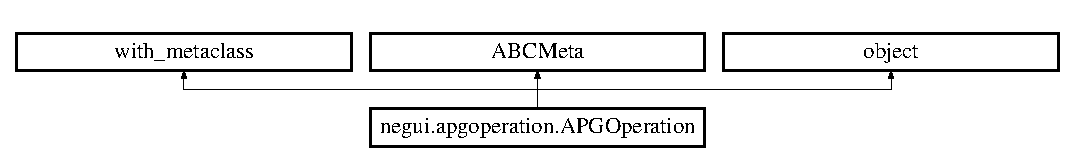
\includegraphics[height=2.000000cm]{classnegui_1_1apgoperation_1_1APGOperation}
\end{center}
\end{figure}
\subsection*{Public Member Functions}
\begin{DoxyCompactItemize}
\item 
def {\bfseries \+\_\+\+\_\+init\+\_\+\+\_\+} (self, o\+\_\+input, o\+\_\+output)\hypertarget{classnegui_1_1apgoperation_1_1APGOperation_a4c8ae262ea950770883a02d8f062bfc1}{}\label{classnegui_1_1apgoperation_1_1APGOperation_a4c8ae262ea950770883a02d8f062bfc1}

\item 
def {\bfseries prepare\+Op} (self)\hypertarget{classnegui_1_1apgoperation_1_1APGOperation_a3167f1a64c3473f000a6268ff6d40955}{}\label{classnegui_1_1apgoperation_1_1APGOperation_a3167f1a64c3473f000a6268ff6d40955}

\item 
def {\bfseries do\+Op} (self)\hypertarget{classnegui_1_1apgoperation_1_1APGOperation_a087b1072a7deae2b98e2c085f0ebebbe}{}\label{classnegui_1_1apgoperation_1_1APGOperation_a087b1072a7deae2b98e2c085f0ebebbe}

\item 
def {\bfseries deliver\+Results} (self)\hypertarget{classnegui_1_1apgoperation_1_1APGOperation_a10f5ecf8d47ef55ba78a8a7a45ad1a6b}{}\label{classnegui_1_1apgoperation_1_1APGOperation_a10f5ecf8d47ef55ba78a8a7a45ad1a6b}

\item 
def {\bfseries input} (self)\hypertarget{classnegui_1_1apgoperation_1_1APGOperation_a7c10319113f046132fe6049896bcd485}{}\label{classnegui_1_1apgoperation_1_1APGOperation_a7c10319113f046132fe6049896bcd485}

\item 
def {\bfseries input} (self, o\+\_\+input\+\_\+object)\hypertarget{classnegui_1_1apgoperation_1_1APGOperation_a44b8970179dccb0e54c3a35463aa5c72}{}\label{classnegui_1_1apgoperation_1_1APGOperation_a44b8970179dccb0e54c3a35463aa5c72}

\item 
def {\bfseries input} (self)\hypertarget{classnegui_1_1apgoperation_1_1APGOperation_a7c10319113f046132fe6049896bcd485}{}\label{classnegui_1_1apgoperation_1_1APGOperation_a7c10319113f046132fe6049896bcd485}

\item 
def {\bfseries output} (self)\hypertarget{classnegui_1_1apgoperation_1_1APGOperation_a70a4663961a30ab0405701072c78f759}{}\label{classnegui_1_1apgoperation_1_1APGOperation_a70a4663961a30ab0405701072c78f759}

\item 
def {\bfseries output} (self, o\+\_\+output\+\_\+object)\hypertarget{classnegui_1_1apgoperation_1_1APGOperation_a92751ec3a6053de0e8638df3d1b122ff}{}\label{classnegui_1_1apgoperation_1_1APGOperation_a92751ec3a6053de0e8638df3d1b122ff}

\item 
def {\bfseries output} (self)\hypertarget{classnegui_1_1apgoperation_1_1APGOperation_a70a4663961a30ab0405701072c78f759}{}\label{classnegui_1_1apgoperation_1_1APGOperation_a70a4663961a30ab0405701072c78f759}

\end{DoxyCompactItemize}


\subsection{Detailed Description}
\begin{DoxyVerb}Abstract class PGOperation is to be implemented by subclasses.
Wraps the code required to perform a pop gen analysis, such as a simuPop simulation,
Or an Ne calculation.  Instantiated subclass objects are the expected type members 
of the PGGuiApp class objects attribute "gp_operation".
\end{DoxyVerb}
 

Definition at line 15 of file apgoperation.\+py.



The documentation for this class was generated from the following file\+:\begin{DoxyCompactItemize}
\item 
apgoperation.\+py\end{DoxyCompactItemize}

\hypertarget{classnegui_1_1pgdriveneestimator_1_1ArgSet}{}\section{negui.\+pgdriveneestimator.\+Arg\+Set Class Reference}
\label{classnegui_1_1pgdriveneestimator_1_1ArgSet}\index{negui.\+pgdriveneestimator.\+Arg\+Set@{negui.\+pgdriveneestimator.\+Arg\+Set}}
Inheritance diagram for negui.\+pgdriveneestimator.\+Arg\+Set\+:\begin{figure}[H]
\begin{center}
\leavevmode
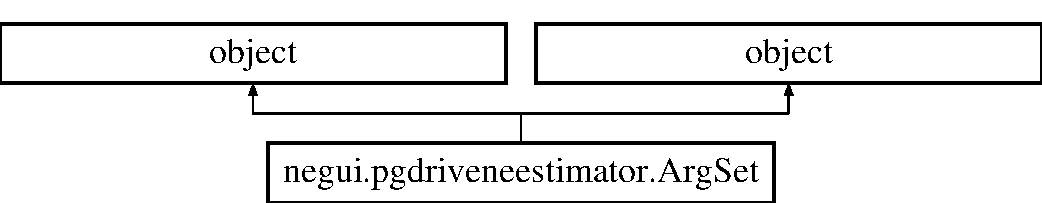
\includegraphics[height=2.000000cm]{classnegui_1_1pgdriveneestimator_1_1ArgSet}
\end{center}
\end{figure}
\subsection*{Public Member Functions}
\begin{DoxyCompactItemize}
\item 
def {\bfseries \+\_\+\+\_\+init\+\_\+\+\_\+} (self, ls\+\_\+args)\hypertarget{classnegui_1_1pgdriveneestimator_1_1ArgSet_af41ba3f691a99548b2027d2d57015535}{}\label{classnegui_1_1pgdriveneestimator_1_1ArgSet_af41ba3f691a99548b2027d2d57015535}

\item 
def {\bfseries paramtable} (self)\hypertarget{classnegui_1_1pgdriveneestimator_1_1ArgSet_a2634d9f265444166815a47bc3a9c8baf}{}\label{classnegui_1_1pgdriveneestimator_1_1ArgSet_a2634d9f265444166815a47bc3a9c8baf}

\item 
def \hyperlink{classnegui_1_1pgdriveneestimator_1_1ArgSet_af060777f11e812d8a1a55b7b1b66cde3}{\+\_\+\+\_\+init\+\_\+\+\_\+} (self, ls\+\_\+args, ls\+\_\+genepop\+\_\+file\+\_\+names=None)
\item 
def {\bfseries genepop\+\_\+file\+\_\+list} (self, ls\+\_\+list)\hypertarget{classnegui_1_1pgdriveneestimator_1_1ArgSet_ae7bf0e1f77c767849fce3e17733cb0b0}{}\label{classnegui_1_1pgdriveneestimator_1_1ArgSet_ae7bf0e1f77c767849fce3e17733cb0b0}

\item 
def {\bfseries paramtable} (self)\hypertarget{classnegui_1_1pgdriveneestimator_1_1ArgSet_a2634d9f265444166815a47bc3a9c8baf}{}\label{classnegui_1_1pgdriveneestimator_1_1ArgSet_a2634d9f265444166815a47bc3a9c8baf}

\end{DoxyCompactItemize}
\subsection*{Public Attributes}
\begin{DoxyCompactItemize}
\item 
{\bfseries param\+\_\+names\+\_\+in\+\_\+order}\hypertarget{classnegui_1_1pgdriveneestimator_1_1ArgSet_a0cdcbc98348d7b15a824518b1e1f61c1}{}\label{classnegui_1_1pgdriveneestimator_1_1ArgSet_a0cdcbc98348d7b15a824518b1e1f61c1}

\item 
{\bfseries arg\+\_\+values}\hypertarget{classnegui_1_1pgdriveneestimator_1_1ArgSet_a2e3b4f2876009bac711cac73863ffd18}{}\label{classnegui_1_1pgdriveneestimator_1_1ArgSet_a2e3b4f2876009bac711cac73863ffd18}

\end{DoxyCompactItemize}


\subsection{Detailed Description}
\begin{DoxyVerb}Wraps list of the arguments and their param names
needed by this driver to do Ne estimations.

Note: this class (a more elaborate version) should have 
been created and used to more extensibly manag
the evaluation and accessability of the argset passed. 
Instead it is only a late addition,
used to print out the arguments to a file (see def 
write_parms_to_file).
\end{DoxyVerb}
 

Definition at line 462 of file pgdriveneestimator.\+experimental.\+py.



\subsection{Constructor \& Destructor Documentation}
\index{negui\+::pgdriveneestimator\+::\+Arg\+Set@{negui\+::pgdriveneestimator\+::\+Arg\+Set}!\+\_\+\+\_\+init\+\_\+\+\_\+@{\+\_\+\+\_\+init\+\_\+\+\_\+}}
\index{\+\_\+\+\_\+init\+\_\+\+\_\+@{\+\_\+\+\_\+init\+\_\+\+\_\+}!negui\+::pgdriveneestimator\+::\+Arg\+Set@{negui\+::pgdriveneestimator\+::\+Arg\+Set}}
\subsubsection[{\texorpdfstring{\+\_\+\+\_\+init\+\_\+\+\_\+(self, ls\+\_\+args, ls\+\_\+genepop\+\_\+file\+\_\+names=\+None)}{__init__(self, ls_args, ls_genepop_file_names=None)}}]{\setlength{\rightskip}{0pt plus 5cm}def negui.\+pgdriveneestimator.\+Arg\+Set.\+\_\+\+\_\+init\+\_\+\+\_\+ (
\begin{DoxyParamCaption}
\item[{}]{self, }
\item[{}]{ls\+\_\+args, }
\item[{}]{ls\+\_\+genepop\+\_\+file\+\_\+names = {\ttfamily None}}
\end{DoxyParamCaption}
)}\hypertarget{classnegui_1_1pgdriveneestimator_1_1ArgSet_af060777f11e812d8a1a55b7b1b66cde3}{}\label{classnegui_1_1pgdriveneestimator_1_1ArgSet_af060777f11e812d8a1a55b7b1b66cde3}
\begin{DoxyVerb}2017_07_11.  We added the ls_genepop_file_names list
and member __genepop_file_list, so that we can report
the actral list of genepop files instead of a glob,
which may have been passed at the command line( See 
def drive_estimator).
\end{DoxyVerb}
 

Definition at line 542 of file pgdriveneestimator.\+py.


\begin{DoxyCode}
542     \textcolor{keyword}{def }\_\_init\_\_( self, ls\_args, ls\_genepop\_file\_names=None ):
543         \textcolor{stringliteral}{'''}
544 \textcolor{stringliteral}{        2017\_07\_11.  We added the ls\_genepop\_file\_names list}
545 \textcolor{stringliteral}{        and member \_\_genepop\_file\_list, so that we can report}
546 \textcolor{stringliteral}{        the actral list of genepop files instead of a glob,}
547 \textcolor{stringliteral}{        which may have been passed at the command line( See }
548 \textcolor{stringliteral}{        def drive\_estimator).}
549 \textcolor{stringliteral}{        '''}
550         self.\hyperlink{classnegui_1_1pgdriveneestimator_1_1ArgSet_a0cdcbc98348d7b15a824518b1e1f61c1}{param\_names\_in\_order}= \(\backslash\)
551                 [ \textcolor{stringliteral}{"genepop\_files"}, \textcolor{stringliteral}{"pop\_sampling\_scheme"},
552                         \textcolor{stringliteral}{"pop\_sampling\_values"},
553                         \textcolor{stringliteral}{"min\_pop\_size"}, \textcolor{stringliteral}{"max\_pop\_size"},
554                         \textcolor{stringliteral}{"pop\_num\_range"}, \textcolor{stringliteral}{"min\_allele\_frequency"},
555                         \textcolor{stringliteral}{"pop\_sampling\_replicates"}, \textcolor{stringliteral}{"loci\_sampling\_scheme"},
556                         \textcolor{stringliteral}{"loci\_sampling\_values"}, \textcolor{stringliteral}{"loci\_min\_total"},
557                         \textcolor{stringliteral}{"loci\_max\_total"}, \textcolor{stringliteral}{"loci\_num\_range"}, 
558                         \textcolor{stringliteral}{"loci\_sampling\_replicates"}, \textcolor{stringliteral}{"total\_cpu\_processes"},
559                         \textcolor{stringliteral}{"debug\_mode"}, \textcolor{stringliteral}{"nbne\_ratio"}, \textcolor{stringliteral}{"do\_nb\_bias\_adjustment"}, \textcolor{stringliteral}{"output\_file"},
560                         \textcolor{stringliteral}{"secondary\_output\_file"} ]
561         
562         \textcolor{comment}{#we make a copy of the arg values:}
563         self.\hyperlink{classnegui_1_1pgdriveneestimator_1_1ArgSet_a2e3b4f2876009bac711cac73863ffd18}{arg\_values}=[ v\_arg \textcolor{keywordflow}{for} v\_arg \textcolor{keywordflow}{in} ls\_args ]
564 
565         self.\hyperlink{classnegui_1_1pgdriveneestimator_1_1ArgSet_aed45ec07079b9956642aa1fc7269e8b9}{\_\_genepop\_file\_list}=ls\_genepop\_file\_names
566         \textcolor{keywordflow}{return}
\end{DoxyCode}


The documentation for this class was generated from the following files\+:\begin{DoxyCompactItemize}
\item 
pgdriveneestimator.\+experimental.\+py\item 
pgdriveneestimator.\+py\end{DoxyCompactItemize}

\hypertarget{classnegui_1_1genepopfilesampler_1_1CohortSamplingValue}{}\section{negui.\+genepopfilesampler.\+Cohort\+Sampling\+Value Class Reference}
\label{classnegui_1_1genepopfilesampler_1_1CohortSamplingValue}\index{negui.\+genepopfilesampler.\+Cohort\+Sampling\+Value@{negui.\+genepopfilesampler.\+Cohort\+Sampling\+Value}}
Inheritance diagram for negui.\+genepopfilesampler.\+Cohort\+Sampling\+Value\+:\begin{figure}[H]
\begin{center}
\leavevmode
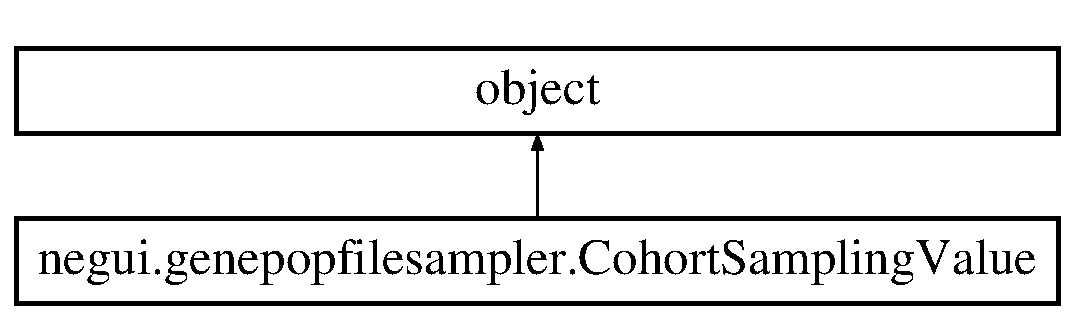
\includegraphics[height=2.000000cm]{classnegui_1_1genepopfilesampler_1_1CohortSamplingValue}
\end{center}
\end{figure}
\subsection*{Public Member Functions}
\begin{DoxyCompactItemize}
\item 
def {\bfseries \+\_\+\+\_\+init\+\_\+\+\_\+} (self, i\+\_\+type, v\+\_\+value)\hypertarget{classnegui_1_1genepopfilesampler_1_1CohortSamplingValue_aaf19161190cabbef80802059770ede18}{}\label{classnegui_1_1genepopfilesampler_1_1CohortSamplingValue_aaf19161190cabbef80802059770ede18}

\item 
def {\bfseries sampling\+\_\+value} (self)\hypertarget{classnegui_1_1genepopfilesampler_1_1CohortSamplingValue_a00a40570f4b1c3e351098bb7d907359c}{}\label{classnegui_1_1genepopfilesampler_1_1CohortSamplingValue_a00a40570f4b1c3e351098bb7d907359c}

\item 
def {\bfseries sampling\+\_\+type} (self)\hypertarget{classnegui_1_1genepopfilesampler_1_1CohortSamplingValue_a873766c4800201f35deaca7064944731}{}\label{classnegui_1_1genepopfilesampler_1_1CohortSamplingValue_a873766c4800201f35deaca7064944731}

\end{DoxyCompactItemize}
\subsection*{Static Public Attributes}
\begin{DoxyCompactItemize}
\item 
int {\bfseries T\+Y\+P\+E\+\_\+\+P\+R\+O\+P\+O\+R\+T\+I\+ON} = 1\hypertarget{classnegui_1_1genepopfilesampler_1_1CohortSamplingValue_affb9d58546e344365b701094e5d3b90f}{}\label{classnegui_1_1genepopfilesampler_1_1CohortSamplingValue_affb9d58546e344365b701094e5d3b90f}

\item 
int {\bfseries T\+Y\+P\+E\+\_\+\+C\+O\+U\+NT} = 2\hypertarget{classnegui_1_1genepopfilesampler_1_1CohortSamplingValue_a0e8231d4ff71b6ffff31eaa0b2d380a1}{}\label{classnegui_1_1genepopfilesampler_1_1CohortSamplingValue_a0e8231d4ff71b6ffff31eaa0b2d380a1}

\item 
int {\bfseries T\+Y\+P\+E\+\_\+\+C\+O\+U\+N\+T\+\_\+\+M\+AX} = 3\hypertarget{classnegui_1_1genepopfilesampler_1_1CohortSamplingValue_a925f70595b847f5908ea731ccc9a0a16}{}\label{classnegui_1_1genepopfilesampler_1_1CohortSamplingValue_a925f70595b847f5908ea731ccc9a0a16}

\end{DoxyCompactItemize}


\subsection{Detailed Description}


Definition at line 50 of file genepopfilesampler.\+py.



The documentation for this class was generated from the following file\+:\begin{DoxyCompactItemize}
\item 
genepopfilesampler.\+py\end{DoxyCompactItemize}

\hypertarget{classnegui_1_1pgdriveneestimator_1_1Counter}{}\section{negui.\+pgdriveneestimator.\+Counter Class Reference}
\label{classnegui_1_1pgdriveneestimator_1_1Counter}\index{negui.\+pgdriveneestimator.\+Counter@{negui.\+pgdriveneestimator.\+Counter}}
Inheritance diagram for negui.\+pgdriveneestimator.\+Counter\+:\begin{figure}[H]
\begin{center}
\leavevmode
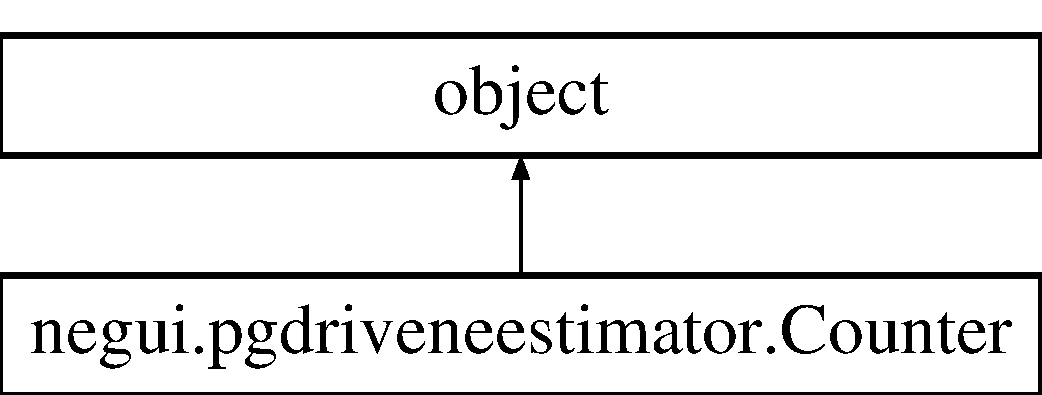
\includegraphics[height=2.000000cm]{classnegui_1_1pgdriveneestimator_1_1Counter}
\end{center}
\end{figure}
\subsection*{Public Member Functions}
\begin{DoxyCompactItemize}
\item 
def {\bfseries \+\_\+\+\_\+init\+\_\+\+\_\+} (self, i\+\_\+init\+\_\+val=0)\hypertarget{classnegui_1_1pgdriveneestimator_1_1Counter_a43f73aa604351514f49c9739855c3be4}{}\label{classnegui_1_1pgdriveneestimator_1_1Counter_a43f73aa604351514f49c9739855c3be4}

\item 
def {\bfseries add\+To\+Current\+Value} (self, i\+\_\+amount\+\_\+to\+\_\+add)\hypertarget{classnegui_1_1pgdriveneestimator_1_1Counter_ac8089b4f487000821321e87144419dc2}{}\label{classnegui_1_1pgdriveneestimator_1_1Counter_ac8089b4f487000821321e87144419dc2}

\item 
def {\bfseries subtract\+From\+Current\+Value} (self, i\+\_\+amount\+\_\+to\+\_\+subtract)\hypertarget{classnegui_1_1pgdriveneestimator_1_1Counter_a448901fbdf9a96bd22c8fafe39d0f0c4}{}\label{classnegui_1_1pgdriveneestimator_1_1Counter_a448901fbdf9a96bd22c8fafe39d0f0c4}

\item 
def {\bfseries reset\+Counter\+To\+Value} (self, i\+\_\+reset\+\_\+value)\hypertarget{classnegui_1_1pgdriveneestimator_1_1Counter_aa52538cc4b8b1712c25f413200f194ea}{}\label{classnegui_1_1pgdriveneestimator_1_1Counter_aa52538cc4b8b1712c25f413200f194ea}

\item 
def {\bfseries current\+\_\+count} (self)\hypertarget{classnegui_1_1pgdriveneestimator_1_1Counter_ab388600a843053d09e0d4b526c6b4314}{}\label{classnegui_1_1pgdriveneestimator_1_1Counter_ab388600a843053d09e0d4b526c6b4314}

\end{DoxyCompactItemize}


\subsection{Detailed Description}
\begin{DoxyVerb}2017_07_05.  Need to pass an object that can increment an int
counter, so that caller gets updated.  This was
motivated by the def file_can_be_added_to_current_set.
\end{DoxyVerb}
 

Definition at line 496 of file pgdriveneestimator.\+py.



The documentation for this class was generated from the following file\+:\begin{DoxyCompactItemize}
\item 
pgdriveneestimator.\+py\end{DoxyCompactItemize}

\hypertarget{classnegui_1_1createtooltip_1_1CreateToolTip}{}\section{negui.\+createtooltip.\+Create\+Tool\+Tip Class Reference}
\label{classnegui_1_1createtooltip_1_1CreateToolTip}\index{negui.\+createtooltip.\+Create\+Tool\+Tip@{negui.\+createtooltip.\+Create\+Tool\+Tip}}
Inheritance diagram for negui.\+createtooltip.\+Create\+Tool\+Tip\+:\begin{figure}[H]
\begin{center}
\leavevmode
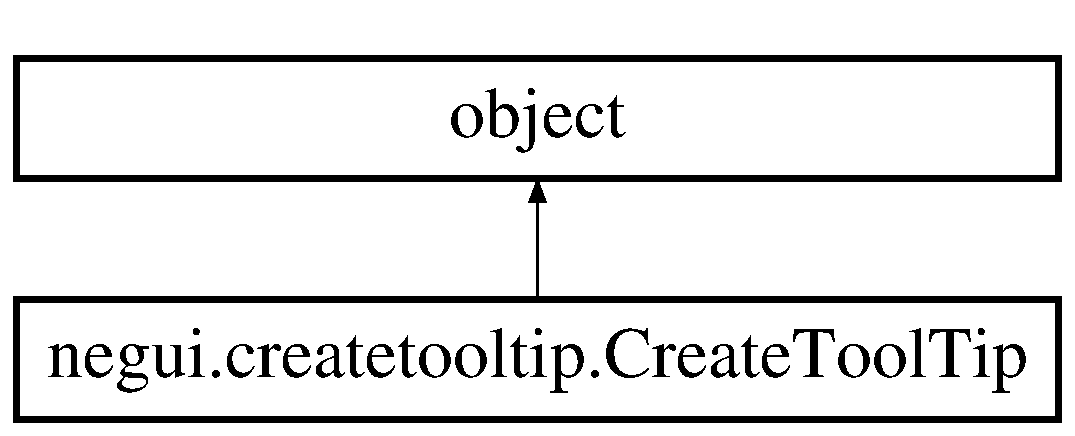
\includegraphics[height=2.000000cm]{classnegui_1_1createtooltip_1_1CreateToolTip}
\end{center}
\end{figure}
\subsection*{Public Member Functions}
\begin{DoxyCompactItemize}
\item 
def \hyperlink{classnegui_1_1createtooltip_1_1CreateToolTip_aec360f7f4bfc95876b04ad68a7c54140}{\+\_\+\+\_\+init\+\_\+\+\_\+} (self, widget, text=\textquotesingle{}widget info\textquotesingle{}, i\+\_\+font\+\_\+size=10)
\item 
def \hyperlink{classnegui_1_1createtooltip_1_1CreateToolTip_ab37624e73833e8ba485d10410c5986bb}{enter} (self, event=None)
\item 
def \hyperlink{classnegui_1_1createtooltip_1_1CreateToolTip_aa6f6887d11b3e07e5f6e12b267412fae}{close} (self, event=None)
\end{DoxyCompactItemize}
\subsection*{Public Attributes}
\begin{DoxyCompactItemize}
\item 
{\bfseries tw}\hypertarget{classnegui_1_1createtooltip_1_1CreateToolTip_ac47a0f82a5a354f6c8914c4631d1a0cf}{}\label{classnegui_1_1createtooltip_1_1CreateToolTip_ac47a0f82a5a354f6c8914c4631d1a0cf}

\item 
{\bfseries widget}\hypertarget{classnegui_1_1createtooltip_1_1CreateToolTip_a6619448e568b135261fd02a6d9b36725}{}\label{classnegui_1_1createtooltip_1_1CreateToolTip_a6619448e568b135261fd02a6d9b36725}

\item 
{\bfseries text}\hypertarget{classnegui_1_1createtooltip_1_1CreateToolTip_a198b3395803def62ec55ed820e756b11}{}\label{classnegui_1_1createtooltip_1_1CreateToolTip_a198b3395803def62ec55ed820e756b11}

\item 
{\bfseries font\+\_\+size}\hypertarget{classnegui_1_1createtooltip_1_1CreateToolTip_a42f2306cb6ad9995d76e0eb556416bed}{}\label{classnegui_1_1createtooltip_1_1CreateToolTip_a42f2306cb6ad9995d76e0eb556416bed}

\end{DoxyCompactItemize}


\subsection{Detailed Description}
\begin{DoxyVerb}Creates a tooltip for a given widget.
This code was copied from 
https://www.daniweb.com/programming/software-development/code/484591/a-tooltip-class-for-tkinter
tk_ToolTip_class101.py
gives a Tkinter widget a tooltip as the mouse is above the widget
tested with Python27 and Python34  by  vegaseat  09sep2014\end{DoxyVerb}
 

Definition at line 38 of file createtooltip.\+py.



\subsection{Constructor \& Destructor Documentation}
\index{negui\+::createtooltip\+::\+Create\+Tool\+Tip@{negui\+::createtooltip\+::\+Create\+Tool\+Tip}!\+\_\+\+\_\+init\+\_\+\+\_\+@{\+\_\+\+\_\+init\+\_\+\+\_\+}}
\index{\+\_\+\+\_\+init\+\_\+\+\_\+@{\+\_\+\+\_\+init\+\_\+\+\_\+}!negui\+::createtooltip\+::\+Create\+Tool\+Tip@{negui\+::createtooltip\+::\+Create\+Tool\+Tip}}
\subsubsection[{\texorpdfstring{\+\_\+\+\_\+init\+\_\+\+\_\+(self, widget, text=\textquotesingle{}widget info\textquotesingle{}, i\+\_\+font\+\_\+size=10)}{__init__(self, widget, text='widget info', i_font_size=10)}}]{\setlength{\rightskip}{0pt plus 5cm}def negui.\+createtooltip.\+Create\+Tool\+Tip.\+\_\+\+\_\+init\+\_\+\+\_\+ (
\begin{DoxyParamCaption}
\item[{}]{self, }
\item[{}]{widget, }
\item[{}]{text = {\ttfamily \textquotesingle{}widget~info\textquotesingle{}}, }
\item[{}]{i\+\_\+font\+\_\+size = {\ttfamily 10}}
\end{DoxyParamCaption}
)}\hypertarget{classnegui_1_1createtooltip_1_1CreateToolTip_aec360f7f4bfc95876b04ad68a7c54140}{}\label{classnegui_1_1createtooltip_1_1CreateToolTip_aec360f7f4bfc95876b04ad68a7c54140}
\begin{DoxyVerb}Ted added, in case close gets called before enter,
we'll have tw inditialzed to None.
\end{DoxyVerb}
 

Definition at line 48 of file createtooltip.\+py.


\begin{DoxyCode}
48     \textcolor{keyword}{def }\hyperlink{classnegui_1_1createtooltip_1_1CreateToolTip_aec360f7f4bfc95876b04ad68a7c54140}{\_\_init\_\_}(self, widget, text='widget info', i\_font\_size=10 ):
49         \textcolor{stringliteral}{'''}
50 \textcolor{stringliteral}{        Ted added, in case close gets called before enter,}
51 \textcolor{stringliteral}{        we'll have tw inditialzed to None.}
52 \textcolor{stringliteral}{        '''}
53         self.\hyperlink{classnegui_1_1createtooltip_1_1CreateToolTip_ac47a0f82a5a354f6c8914c4631d1a0cf}{tw}=\textcolor{keywordtype}{None}
54         self.\hyperlink{classnegui_1_1createtooltip_1_1CreateToolTip_a6619448e568b135261fd02a6d9b36725}{widget} = widget
55         self.\hyperlink{classnegui_1_1createtooltip_1_1CreateToolTip_a198b3395803def62ec55ed820e756b11}{text} = text
56         self.widget.bind(\textcolor{stringliteral}{"<Enter>"}, self.\hyperlink{classnegui_1_1createtooltip_1_1CreateToolTip_ab37624e73833e8ba485d10410c5986bb}{enter})
57         self.widget.bind(\textcolor{stringliteral}{"<Leave>"}, self.\hyperlink{classnegui_1_1createtooltip_1_1CreateToolTip_aa6f6887d11b3e07e5f6e12b267412fae}{close})
58         \textcolor{stringliteral}{'''}
59 \textcolor{stringliteral}{        Trying to fix bug in which tooltop persists}
60 \textcolor{stringliteral}{        permanently.}
61 \textcolor{stringliteral}{        '''}
62         self.widget.bind( \textcolor{stringliteral}{"<FocusOut>"}, self.\hyperlink{classnegui_1_1createtooltip_1_1CreateToolTip_aa6f6887d11b3e07e5f6e12b267412fae}{close})
63         self.\hyperlink{classnegui_1_1createtooltip_1_1CreateToolTip_a42f2306cb6ad9995d76e0eb556416bed}{font\_size}=i\_font\_size
\end{DoxyCode}


\subsection{Member Function Documentation}
\index{negui\+::createtooltip\+::\+Create\+Tool\+Tip@{negui\+::createtooltip\+::\+Create\+Tool\+Tip}!close@{close}}
\index{close@{close}!negui\+::createtooltip\+::\+Create\+Tool\+Tip@{negui\+::createtooltip\+::\+Create\+Tool\+Tip}}
\subsubsection[{\texorpdfstring{close(self, event=\+None)}{close(self, event=None)}}]{\setlength{\rightskip}{0pt plus 5cm}def negui.\+createtooltip.\+Create\+Tool\+Tip.\+close (
\begin{DoxyParamCaption}
\item[{}]{self, }
\item[{}]{event = {\ttfamily None}}
\end{DoxyParamCaption}
)}\hypertarget{classnegui_1_1createtooltip_1_1CreateToolTip_aa6f6887d11b3e07e5f6e12b267412fae}{}\label{classnegui_1_1createtooltip_1_1CreateToolTip_aa6f6887d11b3e07e5f6e12b267412fae}
\begin{DoxyVerb}Code testing and assigning tw for/to None,
added 2016_10_31 to more consistently manage 
the tw member.  See the def "enter",
for more details on some buggy
behavior.
\end{DoxyVerb}
 

Definition at line 110 of file createtooltip.\+py.


\begin{DoxyCode}
110     \textcolor{keyword}{def }\hyperlink{classnegui_1_1createtooltip_1_1CreateToolTip_aa6f6887d11b3e07e5f6e12b267412fae}{close}(self, event=None):
111         \textcolor{stringliteral}{'''}
112 \textcolor{stringliteral}{        Code testing and assigning tw for/to None,}
113 \textcolor{stringliteral}{        added 2016\_10\_31 to more consistently manage }
114 \textcolor{stringliteral}{        the tw member.  See the def "enter",}
115 \textcolor{stringliteral}{        for more details on some buggy}
116 \textcolor{stringliteral}{        behavior.}
117 \textcolor{stringliteral}{        '''}
118         \textcolor{keywordflow}{if} self.\hyperlink{classnegui_1_1createtooltip_1_1CreateToolTip_ac47a0f82a5a354f6c8914c4631d1a0cf}{tw} \textcolor{keywordflow}{is} \textcolor{keywordflow}{not} \textcolor{keywordtype}{None}:
119             self.tw.destroy()
120         \textcolor{comment}{#end if}
121 
122         \textcolor{stringliteral}{'''}
123 \textcolor{stringliteral}{        Consistent value for tw after call}
124 \textcolor{stringliteral}{        to close, no matter its previous one:}
125 \textcolor{stringliteral}{        '''}
126         self.\hyperlink{classnegui_1_1createtooltip_1_1CreateToolTip_ac47a0f82a5a354f6c8914c4631d1a0cf}{tw} = \textcolor{keywordtype}{None}
\end{DoxyCode}
\index{negui\+::createtooltip\+::\+Create\+Tool\+Tip@{negui\+::createtooltip\+::\+Create\+Tool\+Tip}!enter@{enter}}
\index{enter@{enter}!negui\+::createtooltip\+::\+Create\+Tool\+Tip@{negui\+::createtooltip\+::\+Create\+Tool\+Tip}}
\subsubsection[{\texorpdfstring{enter(self, event=\+None)}{enter(self, event=None)}}]{\setlength{\rightskip}{0pt plus 5cm}def negui.\+createtooltip.\+Create\+Tool\+Tip.\+enter (
\begin{DoxyParamCaption}
\item[{}]{self, }
\item[{}]{event = {\ttfamily None}}
\end{DoxyParamCaption}
)}\hypertarget{classnegui_1_1createtooltip_1_1CreateToolTip_ab37624e73833e8ba485d10410c5986bb}{}\label{classnegui_1_1createtooltip_1_1CreateToolTip_ab37624e73833e8ba485d10410c5986bb}
\begin{DoxyVerb}Code added 2016_10_31, setting the tw member 
to None in __init__ (see above), then always 
testing it before recreating it, seems to have
resolved a bug, seemingly only associated with
comboboxes and very rarely with text boxes,
via my KeyVal objects, in which the tooltip
window was created but never closed.  This
was reliably invoked by using the keyboard
to update a combobox, while the mouse was still
over the control. On th ekeyboard selection, the
tooltip windows would appear and persist, while
new ones would appear over it.  This management
and testing of the tw member seems to have solved
it.
\end{DoxyVerb}
 

Definition at line 66 of file createtooltip.\+py.


\begin{DoxyCode}
66     \textcolor{keyword}{def }\hyperlink{classnegui_1_1createtooltip_1_1CreateToolTip_ab37624e73833e8ba485d10410c5986bb}{enter}(self, event=None):
67 
68         \textcolor{stringliteral}{'''}
69 \textcolor{stringliteral}{        Code added 2016\_10\_31, setting the tw member }
70 \textcolor{stringliteral}{        to None in \_\_init\_\_ (see above), then always }
71 \textcolor{stringliteral}{        testing it before recreating it, seems to have}
72 \textcolor{stringliteral}{        resolved a bug, seemingly only associated with}
73 \textcolor{stringliteral}{        comboboxes and very rarely with text boxes,}
74 \textcolor{stringliteral}{        via my KeyVal objects, in which the tooltip}
75 \textcolor{stringliteral}{        window was created but never closed.  This}
76 \textcolor{stringliteral}{        was reliably invoked by using the keyboard}
77 \textcolor{stringliteral}{        to update a combobox, while the mouse was still}
78 \textcolor{stringliteral}{        over the control. On th ekeyboard selection, the}
79 \textcolor{stringliteral}{        tooltip windows would appear and persist, while}
80 \textcolor{stringliteral}{        new ones would appear over it.  This management}
81 \textcolor{stringliteral}{        and testing of the tw member seems to have solved}
82 \textcolor{stringliteral}{        it.}
83 \textcolor{stringliteral}{        '''}
84         \textcolor{keywordflow}{if} self.\hyperlink{classnegui_1_1createtooltip_1_1CreateToolTip_ac47a0f82a5a354f6c8914c4631d1a0cf}{tw} \textcolor{keywordflow}{is} \textcolor{keywordtype}{None}:
85             \textcolor{stringliteral}{'''}
86 \textcolor{stringliteral}{            I added 2016\_10\_31}
87 \textcolor{stringliteral}{            constants used below,}
88 \textcolor{stringliteral}{            instead of literals,}
89 \textcolor{stringliteral}{            '''} 
90             PADX=25
91             PADY=20
92 
93             x = y = 0
94             x, y, cx, cy = self.widget.bbox(\textcolor{stringliteral}{"insert"})
95             x += self.widget.winfo\_rootx() + PADX
96             y += self.widget.winfo\_rooty() + PADY
97             \textcolor{comment}{# creates a toplevel window}
98             self.\hyperlink{classnegui_1_1createtooltip_1_1CreateToolTip_ac47a0f82a5a354f6c8914c4631d1a0cf}{tw} = tk.Toplevel(self.\hyperlink{classnegui_1_1createtooltip_1_1CreateToolTip_a6619448e568b135261fd02a6d9b36725}{widget})
99             \textcolor{comment}{# Leaves only the label and removes the app window}
100             self.tw.wm\_overrideredirect(\textcolor{keyword}{True})
101             self.tw.wm\_geometry(\textcolor{stringliteral}{"+%d+%d"} % (x, y))
102             label = tk.Label(self.\hyperlink{classnegui_1_1createtooltip_1_1CreateToolTip_ac47a0f82a5a354f6c8914c4631d1a0cf}{tw}, text=self.\hyperlink{classnegui_1_1createtooltip_1_1CreateToolTip_a198b3395803def62ec55ed820e756b11}{text}, justify=\textcolor{stringliteral}{'left'},
103                            background=\textcolor{stringliteral}{'yellow'}, relief=\textcolor{stringliteral}{'solid'}, borderwidth=1,
104                            font=(\textcolor{stringliteral}{"times"}, self.\hyperlink{classnegui_1_1createtooltip_1_1CreateToolTip_a42f2306cb6ad9995d76e0eb556416bed}{font\_size}, \textcolor{stringliteral}{"normal"}))
105             label.pack(ipadx=1)
106         \textcolor{comment}{#end if self.tw is  None}
107 
\end{DoxyCode}


The documentation for this class was generated from the following file\+:\begin{DoxyCompactItemize}
\item 
createtooltip.\+py\end{DoxyCompactItemize}

\hypertarget{classnegui_1_1pgdriveneestimator_1_1DebugMode}{}\section{negui.\+pgdriveneestimator.\+Debug\+Mode Class Reference}
\label{classnegui_1_1pgdriveneestimator_1_1DebugMode}\index{negui.\+pgdriveneestimator.\+Debug\+Mode@{negui.\+pgdriveneestimator.\+Debug\+Mode}}
Inheritance diagram for negui.\+pgdriveneestimator.\+Debug\+Mode\+:\begin{figure}[H]
\begin{center}
\leavevmode
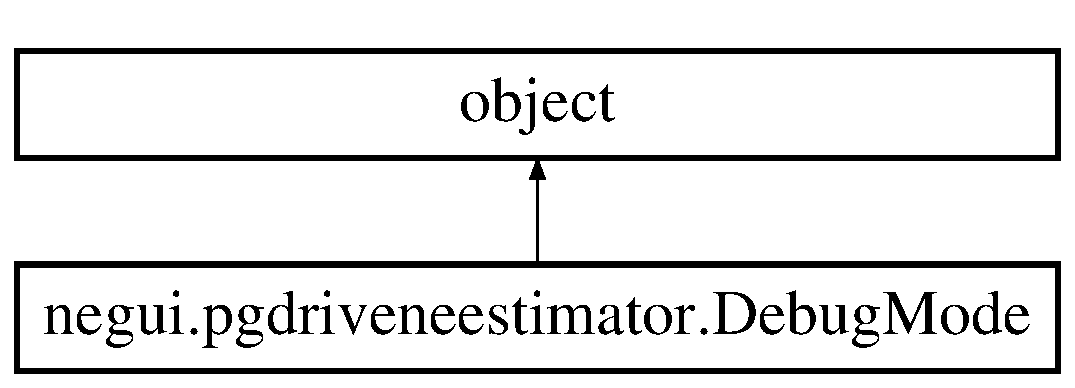
\includegraphics[height=2.000000cm]{classnegui_1_1pgdriveneestimator_1_1DebugMode}
\end{center}
\end{figure}
\subsection*{Public Member Functions}
\begin{DoxyCompactItemize}
\item 
def {\bfseries \+\_\+\+\_\+init\+\_\+\+\_\+} (self, s\+\_\+mode=\char`\"{}no\+\_\+debug\char`\"{})\hypertarget{classnegui_1_1pgdriveneestimator_1_1DebugMode_ad28ea39a3d3a4163f408348fbcdf8207}{}\label{classnegui_1_1pgdriveneestimator_1_1DebugMode_ad28ea39a3d3a4163f408348fbcdf8207}

\item 
def {\bfseries is\+Set} (self, i\+\_\+flag)\hypertarget{classnegui_1_1pgdriveneestimator_1_1DebugMode_ab345367b1debb52518dd753b4c740d3c}{}\label{classnegui_1_1pgdriveneestimator_1_1DebugMode_ab345367b1debb52518dd753b4c740d3c}

\item 
def {\bfseries mode} (self)\hypertarget{classnegui_1_1pgdriveneestimator_1_1DebugMode_a877126bd7e0e8a571b90e0be7436568b}{}\label{classnegui_1_1pgdriveneestimator_1_1DebugMode_a877126bd7e0e8a571b90e0be7436568b}

\item 
def {\bfseries mode} (self, s\+\_\+mode)\hypertarget{classnegui_1_1pgdriveneestimator_1_1DebugMode_ae3f4deed085cffa67a10aa94f857ade0}{}\label{classnegui_1_1pgdriveneestimator_1_1DebugMode_ae3f4deed085cffa67a10aa94f857ade0}

\end{DoxyCompactItemize}
\subsection*{Static Public Attributes}
\begin{DoxyCompactItemize}
\item 
list {\bfseries M\+O\+D\+ES} = \mbox{[} \char`\"{}no\+\_\+debug\char`\"{}, \char`\"{}debug1\char`\"{}, \char`\"{}debug2\char`\"{}, \char`\"{}debug3\char`\"{}, \char`\"{}testserial\char`\"{}, \char`\"{}testmulti\char`\"{} \mbox{]}\hypertarget{classnegui_1_1pgdriveneestimator_1_1DebugMode_a7f3d898bacc395557b8cb40337cfa7e6}{}\label{classnegui_1_1pgdriveneestimator_1_1DebugMode_a7f3d898bacc395557b8cb40337cfa7e6}

\item 
string {\bfseries N\+O\+\_\+\+D\+E\+B\+UG} = \char`\"{}no\+\_\+debug\char`\"{}\hypertarget{classnegui_1_1pgdriveneestimator_1_1DebugMode_a68f03775793d9894bdb28c34f9b33a0c}{}\label{classnegui_1_1pgdriveneestimator_1_1DebugMode_a68f03775793d9894bdb28c34f9b33a0c}

\item 
string {\bfseries M\+A\+K\+E\+\_\+\+T\+A\+B\+LE} = \char`\"{}debug1\char`\"{}\hypertarget{classnegui_1_1pgdriveneestimator_1_1DebugMode_ad287b36021099229f7f4fc86ebc5774e}{}\label{classnegui_1_1pgdriveneestimator_1_1DebugMode_ad287b36021099229f7f4fc86ebc5774e}

\item 
string {\bfseries M\+A\+K\+E\+\_\+\+T\+A\+B\+L\+E\+\_\+\+A\+N\+D\+\_\+\+K\+E\+E\+P\+\_\+\+F\+I\+L\+ES} = \char`\"{}debug2\char`\"{}\hypertarget{classnegui_1_1pgdriveneestimator_1_1DebugMode_a9fb4c700600776a72a359483a08928ea}{}\label{classnegui_1_1pgdriveneestimator_1_1DebugMode_a9fb4c700600776a72a359483a08928ea}

\item 
string {\bfseries A\+L\+L\+\_\+\+D\+E\+B\+U\+G\+\_\+\+O\+P\+T\+I\+O\+NS} = \char`\"{}debug3\char`\"{}\hypertarget{classnegui_1_1pgdriveneestimator_1_1DebugMode_a9f3faea66935c3978c447de9baf0f144}{}\label{classnegui_1_1pgdriveneestimator_1_1DebugMode_a9f3faea66935c3978c447de9baf0f144}

\item 
string {\bfseries T\+E\+S\+T\+\_\+\+S\+E\+R\+I\+AL} = \char`\"{}testserial\char`\"{}\hypertarget{classnegui_1_1pgdriveneestimator_1_1DebugMode_aec7b522f17d7790b980ae128a4445b0e}{}\label{classnegui_1_1pgdriveneestimator_1_1DebugMode_aec7b522f17d7790b980ae128a4445b0e}

\item 
string {\bfseries T\+E\+S\+T\+\_\+\+M\+U\+L\+TI} = \char`\"{}testmulti\char`\"{}\hypertarget{classnegui_1_1pgdriveneestimator_1_1DebugMode_a8a5f8c6fe20337dd6b894aba21bd1e17}{}\label{classnegui_1_1pgdriveneestimator_1_1DebugMode_a8a5f8c6fe20337dd6b894aba21bd1e17}

\item 
int {\bfseries K\+E\+E\+P\+\_\+\+R\+E\+P\+L\+I\+C\+A\+T\+E\+\_\+\+G\+E\+N\+E\+P\+O\+P\+\_\+\+F\+I\+L\+ES} = 1\hypertarget{classnegui_1_1pgdriveneestimator_1_1DebugMode_a28d1c7693a4bec8f391bef360d51b463}{}\label{classnegui_1_1pgdriveneestimator_1_1DebugMode_a28d1c7693a4bec8f391bef360d51b463}

\item 
int {\bfseries K\+E\+E\+P\+\_\+\+E\+S\+T\+I\+M\+A\+T\+O\+R\+\_\+\+F\+I\+L\+ES} = 2\hypertarget{classnegui_1_1pgdriveneestimator_1_1DebugMode_a2f02d51f5d3a4a6c9cfaa8d0f6ea1879}{}\label{classnegui_1_1pgdriveneestimator_1_1DebugMode_a2f02d51f5d3a4a6c9cfaa8d0f6ea1879}

\item 
int {\bfseries M\+A\+K\+E\+\_\+\+I\+N\+D\+I\+V\+\_\+\+T\+A\+B\+LE} = 4\hypertarget{classnegui_1_1pgdriveneestimator_1_1DebugMode_a1f5d7e71208d6a4a9d7a63b0207e1ab8}{}\label{classnegui_1_1pgdriveneestimator_1_1DebugMode_a1f5d7e71208d6a4a9d7a63b0207e1ab8}

\item 
int {\bfseries A\+L\+L\+O\+W\+\_\+\+M\+U\+L\+T\+I\+\_\+\+P\+R\+O\+C\+E\+S\+S\+ES} = 8\hypertarget{classnegui_1_1pgdriveneestimator_1_1DebugMode_af0b037fef1711a912d1f83ed61f57097}{}\label{classnegui_1_1pgdriveneestimator_1_1DebugMode_af0b037fef1711a912d1f83ed61f57097}

\item 
int {\bfseries P\+R\+I\+N\+T\+\_\+\+R\+E\+P\+L\+I\+C\+A\+T\+E\+\_\+\+S\+E\+L\+E\+C\+T\+I\+O\+NS} = 16\hypertarget{classnegui_1_1pgdriveneestimator_1_1DebugMode_a238432e744ac313e2ce4d7de801ffe92}{}\label{classnegui_1_1pgdriveneestimator_1_1DebugMode_a238432e744ac313e2ce4d7de801ffe92}

\item 
int {\bfseries K\+E\+E\+P\+\_\+\+N\+O\+D\+A\+T\+\_\+\+F\+I\+L\+ES} = 32\hypertarget{classnegui_1_1pgdriveneestimator_1_1DebugMode_ac55e866ab4d12b084f2480d625c9dbb8}{}\label{classnegui_1_1pgdriveneestimator_1_1DebugMode_ac55e866ab4d12b084f2480d625c9dbb8}

\item 
int {\bfseries K\+E\+E\+P\+\_\+\+N\+E\+X\+T\+P\+\_\+\+F\+I\+L\+ES} = 64\hypertarget{classnegui_1_1pgdriveneestimator_1_1DebugMode_a13096a90911741639b1eea0e1595cb2b}{}\label{classnegui_1_1pgdriveneestimator_1_1DebugMode_a13096a90911741639b1eea0e1595cb2b}

\end{DoxyCompactItemize}


\subsection{Detailed Description}


Definition at line 273 of file pgdriveneestimator.\+py.



The documentation for this class was generated from the following file\+:\begin{DoxyCompactItemize}
\item 
pgdriveneestimator.\+py\end{DoxyCompactItemize}

\hypertarget{classnegui_1_1pgutilityclasses_1_1FloatIntStringParamValidity}{}\section{negui.\+pgutilityclasses.\+Float\+Int\+String\+Param\+Validity Class Reference}
\label{classnegui_1_1pgutilityclasses_1_1FloatIntStringParamValidity}\index{negui.\+pgutilityclasses.\+Float\+Int\+String\+Param\+Validity@{negui.\+pgutilityclasses.\+Float\+Int\+String\+Param\+Validity}}
Inheritance diagram for negui.\+pgutilityclasses.\+Float\+Int\+String\+Param\+Validity\+:\begin{figure}[H]
\begin{center}
\leavevmode
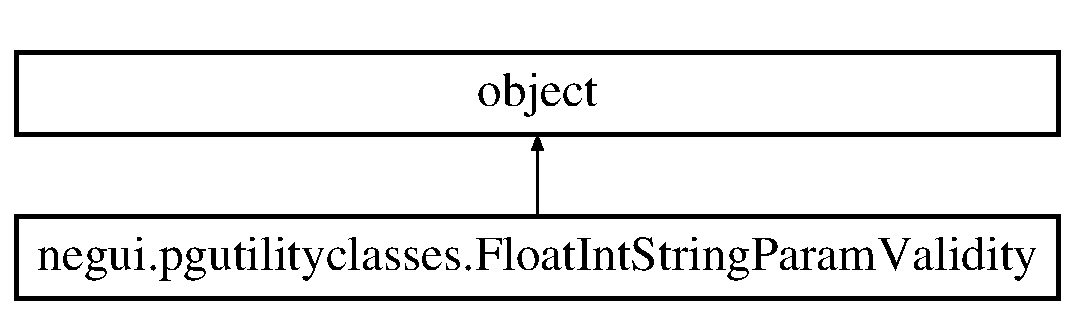
\includegraphics[height=2.000000cm]{classnegui_1_1pgutilityclasses_1_1FloatIntStringParamValidity}
\end{center}
\end{figure}
\subsection*{Public Member Functions}
\begin{DoxyCompactItemize}
\item 
def {\bfseries \+\_\+\+\_\+init\+\_\+\+\_\+} (self, s\+\_\+name, o\+\_\+type, o\+\_\+value, i\+\_\+min\+\_\+value=None, i\+\_\+max\+\_\+value=None)\hypertarget{classnegui_1_1pgutilityclasses_1_1FloatIntStringParamValidity_aca9afc3100b25bfbbe4807d66dfed872}{}\label{classnegui_1_1pgutilityclasses_1_1FloatIntStringParamValidity_aca9afc3100b25bfbbe4807d66dfed872}

\item 
def {\bfseries is\+Valid} (self)\hypertarget{classnegui_1_1pgutilityclasses_1_1FloatIntStringParamValidity_ae4f8588a74ee6757f49a8a6f2bef9a85}{}\label{classnegui_1_1pgutilityclasses_1_1FloatIntStringParamValidity_ae4f8588a74ee6757f49a8a6f2bef9a85}

\item 
def {\bfseries report\+Validity} (self)\hypertarget{classnegui_1_1pgutilityclasses_1_1FloatIntStringParamValidity_a5f14ea6b63e3175ccb728b12520bb142}{}\label{classnegui_1_1pgutilityclasses_1_1FloatIntStringParamValidity_a5f14ea6b63e3175ccb728b12520bb142}

\item 
def {\bfseries report\+Invalidity\+Only} (self)\hypertarget{classnegui_1_1pgutilityclasses_1_1FloatIntStringParamValidity_acae489553a6e2295b527622809843275}{}\label{classnegui_1_1pgutilityclasses_1_1FloatIntStringParamValidity_acae489553a6e2295b527622809843275}

\item 
def {\bfseries value} (self)\hypertarget{classnegui_1_1pgutilityclasses_1_1FloatIntStringParamValidity_a39a4e8fc867e88dc3fb0b8852f01bf24}{}\label{classnegui_1_1pgutilityclasses_1_1FloatIntStringParamValidity_a39a4e8fc867e88dc3fb0b8852f01bf24}

\item 
def {\bfseries value} (self, v\+\_\+value)\hypertarget{classnegui_1_1pgutilityclasses_1_1FloatIntStringParamValidity_a71a6b9ac6c7ed230dfc4c474882f8708}{}\label{classnegui_1_1pgutilityclasses_1_1FloatIntStringParamValidity_a71a6b9ac6c7ed230dfc4c474882f8708}

\end{DoxyCompactItemize}


\subsection{Detailed Description}
\begin{DoxyVerb}For validation checks on a parameter value
before it is used to run an analysis.
\end{DoxyVerb}
 

Definition at line 127 of file pgutilityclasses.\+py.



The documentation for this class was generated from the following file\+:\begin{DoxyCompactItemize}
\item 
pgutilityclasses.\+py\end{DoxyCompactItemize}

\hypertarget{classnegui_1_1pgframecontainerscrolled_1_1FrameContainerScrolled}{}\section{negui.\+pgframecontainerscrolled.\+Frame\+Container\+Scrolled Class Reference}
\label{classnegui_1_1pgframecontainerscrolled_1_1FrameContainerScrolled}\index{negui.\+pgframecontainerscrolled.\+Frame\+Container\+Scrolled@{negui.\+pgframecontainerscrolled.\+Frame\+Container\+Scrolled}}
Inheritance diagram for negui.\+pgframecontainerscrolled.\+Frame\+Container\+Scrolled\+:\begin{figure}[H]
\begin{center}
\leavevmode
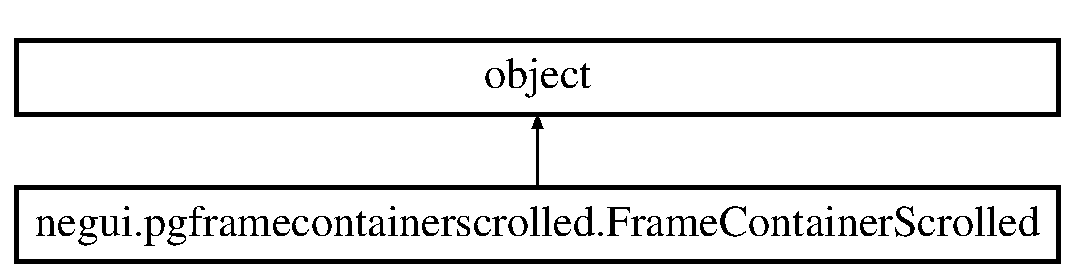
\includegraphics[height=2.000000cm]{classnegui_1_1pgframecontainerscrolled_1_1FrameContainerScrolled}
\end{center}
\end{figure}
\subsection*{Public Member Functions}
\begin{DoxyCompactItemize}
\item 
def {\bfseries \+\_\+\+\_\+init\+\_\+\+\_\+} (self, o\+\_\+parent\+\_\+frame, o\+\_\+child\+\_\+frame, o\+\_\+canvas, i\+\_\+scroll\+\_\+direction=S\+C\+R\+O\+L\+L\+V\+E\+R\+T\+I\+C\+AL)\hypertarget{classnegui_1_1pgframecontainerscrolled_1_1FrameContainerScrolled_a9a522fc76132e89237920a9878e826d1}{}\label{classnegui_1_1pgframecontainerscrolled_1_1FrameContainerScrolled_a9a522fc76132e89237920a9878e826d1}

\item 
def \hyperlink{classnegui_1_1pgframecontainerscrolled_1_1FrameContainerScrolled_a4de903801fd0962b403d29b1653b07c2}{rebind\+Scrollwheel} (self)
\end{DoxyCompactItemize}
\subsection*{Static Public Attributes}
\begin{DoxyCompactItemize}
\item 
int {\bfseries S\+C\+R\+O\+L\+L\+V\+E\+R\+T\+I\+C\+AL} = 0\hypertarget{classnegui_1_1pgframecontainerscrolled_1_1FrameContainerScrolled_a9f8fc6bb77d2973ee318f146b2da7faf}{}\label{classnegui_1_1pgframecontainerscrolled_1_1FrameContainerScrolled_a9f8fc6bb77d2973ee318f146b2da7faf}

\item 
int {\bfseries S\+C\+R\+O\+L\+L\+H\+O\+R\+I\+Z\+O\+N\+T\+AL} = 1\hypertarget{classnegui_1_1pgframecontainerscrolled_1_1FrameContainerScrolled_a9892a6bde66588412759262fb7d10f95}{}\label{classnegui_1_1pgframecontainerscrolled_1_1FrameContainerScrolled_a9892a6bde66588412759262fb7d10f95}

\item 
int {\bfseries S\+C\+R\+O\+L\+L\+B\+O\+TH} = 2\hypertarget{classnegui_1_1pgframecontainerscrolled_1_1FrameContainerScrolled_a6b07c9a74064e855296e4f9289b5b765}{}\label{classnegui_1_1pgframecontainerscrolled_1_1FrameContainerScrolled_a6b07c9a74064e855296e4f9289b5b765}

\end{DoxyCompactItemize}


\subsection{Detailed Description}
\begin{DoxyVerb}Description
Objects are arrangements of two Frames and a 
Canvas, such that one frame contains the 
canvas and 2nd frame, and the 2nd frame 
is scrollable, either vertically or horizontally 
(but not yet both, as of Thu Jun  2 19:59:32 MDT 2016 )


Note that this is not a Tkinter object, but
simply accomplishes the arragnement. 

Note that this uses Fred Lundh's AutoScrollbar class
(from http://effbot.org/zone/tkinter-autoscrollbar.htm)
and depends on using only the grid geometry manager to place
the scrollbar.
\end{DoxyVerb}
 

Definition at line 27 of file pgframecontainerscrolled.\+py.



\subsection{Member Function Documentation}
\index{negui\+::pgframecontainerscrolled\+::\+Frame\+Container\+Scrolled@{negui\+::pgframecontainerscrolled\+::\+Frame\+Container\+Scrolled}!rebind\+Scrollwheel@{rebind\+Scrollwheel}}
\index{rebind\+Scrollwheel@{rebind\+Scrollwheel}!negui\+::pgframecontainerscrolled\+::\+Frame\+Container\+Scrolled@{negui\+::pgframecontainerscrolled\+::\+Frame\+Container\+Scrolled}}
\subsubsection[{\texorpdfstring{rebind\+Scrollwheel(self)}{rebindScrollwheel(self)}}]{\setlength{\rightskip}{0pt plus 5cm}def negui.\+pgframecontainerscrolled.\+Frame\+Container\+Scrolled.\+rebind\+Scrollwheel (
\begin{DoxyParamCaption}
\item[{}]{self}
\end{DoxyParamCaption}
)}\hypertarget{classnegui_1_1pgframecontainerscrolled_1_1FrameContainerScrolled_a4de903801fd0962b403d29b1653b07c2}{}\label{classnegui_1_1pgframecontainerscrolled_1_1FrameContainerScrolled_a4de903801fd0962b403d29b1653b07c2}
\begin{DoxyVerb}This def allows clients to rebind the mouse scrollwheel
to this object's canvas.  This was necessitated by
tab swithes in the pghostnotebook.py class object,
which casue the mouse wheel to be bound to the latest
tab, and "disconnects" it from all others, so that,
returning to an older tab, gives an inteface without
mouse wheel scrolling enabled.
\end{DoxyVerb}
 

Definition at line 138 of file pgframecontainerscrolled.\+py.


\begin{DoxyCode}
138     \textcolor{keyword}{def }\hyperlink{classnegui_1_1pgframecontainerscrolled_1_1FrameContainerScrolled_a4de903801fd0962b403d29b1653b07c2}{rebindScrollwheel}(self):
139         \textcolor{stringliteral}{'''}
140 \textcolor{stringliteral}{        This def allows clients to rebind the mouse scrollwheel}
141 \textcolor{stringliteral}{        to this object's canvas.  This was necessitated by}
142 \textcolor{stringliteral}{        tab swithes in the pghostnotebook.py class object,}
143 \textcolor{stringliteral}{        which casue the mouse wheel to be bound to the latest}
144 \textcolor{stringliteral}{        tab, and "disconnects" it from all others, so that,}
145 \textcolor{stringliteral}{        returning to an older tab, gives an inteface without}
146 \textcolor{stringliteral}{        mouse wheel scrolling enabled.}
147 \textcolor{stringliteral}{        '''}
148 
149         self.\hyperlink{classnegui_1_1pgframecontainerscrolled_1_1FrameContainerScrolled_acddb919ce697114d9dab8570c8c96ba6}{\_\_bind\_canvas\_to\_scrollwheel}()
150         \textcolor{keywordflow}{return}
\end{DoxyCode}


The documentation for this class was generated from the following file\+:\begin{DoxyCompactItemize}
\item 
pgframecontainerscrolled.\+py\end{DoxyCompactItemize}

\hypertarget{classnegui_1_1pgguiutilities_1_1FrameContainerVScroll}{}\section{negui.\+pgguiutilities.\+Frame\+Container\+V\+Scroll Class Reference}
\label{classnegui_1_1pgguiutilities_1_1FrameContainerVScroll}\index{negui.\+pgguiutilities.\+Frame\+Container\+V\+Scroll@{negui.\+pgguiutilities.\+Frame\+Container\+V\+Scroll}}
Inheritance diagram for negui.\+pgguiutilities.\+Frame\+Container\+V\+Scroll\+:\begin{figure}[H]
\begin{center}
\leavevmode
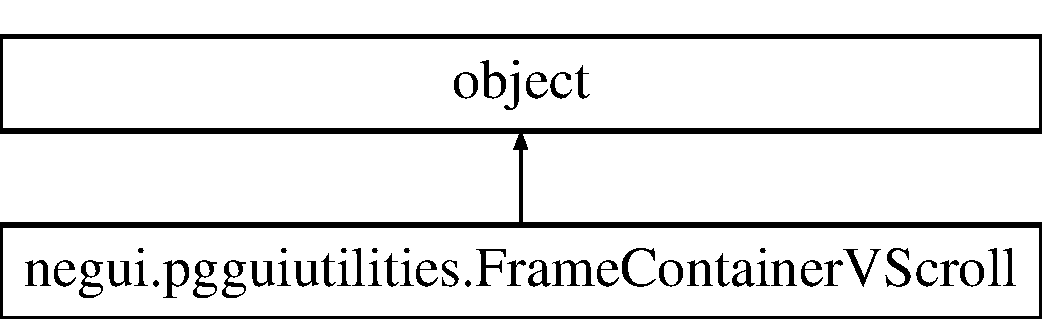
\includegraphics[height=2.000000cm]{classnegui_1_1pgguiutilities_1_1FrameContainerVScroll}
\end{center}
\end{figure}
\subsection*{Public Member Functions}
\begin{DoxyCompactItemize}
\item 
def {\bfseries \+\_\+\+\_\+init\+\_\+\+\_\+} (self, o\+\_\+parent\+\_\+frame, o\+\_\+child\+\_\+frame, o\+\_\+canvas)\hypertarget{classnegui_1_1pgguiutilities_1_1FrameContainerVScroll_a77671bf20cb4175f0788de78bda3445f}{}\label{classnegui_1_1pgguiutilities_1_1FrameContainerVScroll_a77671bf20cb4175f0788de78bda3445f}

\end{DoxyCompactItemize}


\subsection{Detailed Description}
\begin{DoxyVerb}Description
Objects are arrangements of two Frames and a 
Canvas, such that one frame contains the 
canvas and 2nd frame, and the 2nd frame 
is vertically scrollable.

Note that this is not a Tkinter object, but
simply accomplishes the arragnement. 

Note that this uses Fred Lundh's AutoScrollbar class
(from http://effbot.org/zone/tkinter-autoscrollbar.htm)
and depends on using only the grid geometry manager to place
the scrollbar.
\end{DoxyVerb}
 

Definition at line 1277 of file pgguiutilities.\+py.



The documentation for this class was generated from the following file\+:\begin{DoxyCompactItemize}
\item 
pgguiutilities.\+py\end{DoxyCompactItemize}

\hypertarget{classnegui_1_1pgguiutilities_1_1FredLundhsAutoScrollbar}{}\section{negui.\+pgguiutilities.\+Fred\+Lundhs\+Auto\+Scrollbar Class Reference}
\label{classnegui_1_1pgguiutilities_1_1FredLundhsAutoScrollbar}\index{negui.\+pgguiutilities.\+Fred\+Lundhs\+Auto\+Scrollbar@{negui.\+pgguiutilities.\+Fred\+Lundhs\+Auto\+Scrollbar}}
Inheritance diagram for negui.\+pgguiutilities.\+Fred\+Lundhs\+Auto\+Scrollbar\+:\begin{figure}[H]
\begin{center}
\leavevmode
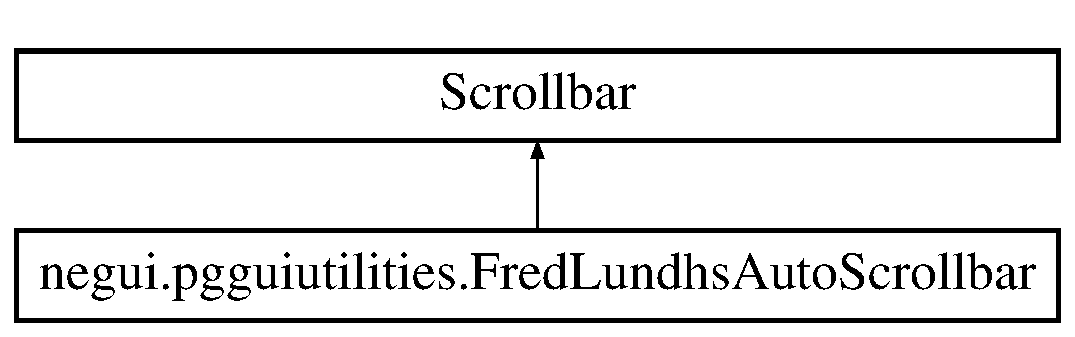
\includegraphics[height=2.000000cm]{classnegui_1_1pgguiutilities_1_1FredLundhsAutoScrollbar}
\end{center}
\end{figure}
\subsection*{Public Member Functions}
\begin{DoxyCompactItemize}
\item 
def {\bfseries set} (self, lo, hi)\hypertarget{classnegui_1_1pgguiutilities_1_1FredLundhsAutoScrollbar_aba2e2b98ba2b20fe53fed36d35295acb}{}\label{classnegui_1_1pgguiutilities_1_1FredLundhsAutoScrollbar_aba2e2b98ba2b20fe53fed36d35295acb}

\item 
def {\bfseries pack} (self, kw)\hypertarget{classnegui_1_1pgguiutilities_1_1FredLundhsAutoScrollbar_ab584fb578f832316f881cfdd4ed157e7}{}\label{classnegui_1_1pgguiutilities_1_1FredLundhsAutoScrollbar_ab584fb578f832316f881cfdd4ed157e7}

\item 
def {\bfseries place} (self, kw)\hypertarget{classnegui_1_1pgguiutilities_1_1FredLundhsAutoScrollbar_a5b729724cf7818ec6776fdfee6104fb8}{}\label{classnegui_1_1pgguiutilities_1_1FredLundhsAutoScrollbar_a5b729724cf7818ec6776fdfee6104fb8}

\end{DoxyCompactItemize}


\subsection{Detailed Description}


Definition at line 33 of file pgguiutilities.\+py.



The documentation for this class was generated from the following file\+:\begin{DoxyCompactItemize}
\item 
pgguiutilities.\+py\end{DoxyCompactItemize}

\hypertarget{classnegui_1_1genepopfilelociinfo_1_1GenepopFileLociInfo}{}\section{negui.\+genepopfilelociinfo.\+Genepop\+File\+Loci\+Info Class Reference}
\label{classnegui_1_1genepopfilelociinfo_1_1GenepopFileLociInfo}\index{negui.\+genepopfilelociinfo.\+Genepop\+File\+Loci\+Info@{negui.\+genepopfilelociinfo.\+Genepop\+File\+Loci\+Info}}
Inheritance diagram for negui.\+genepopfilelociinfo.\+Genepop\+File\+Loci\+Info\+:\begin{figure}[H]
\begin{center}
\leavevmode
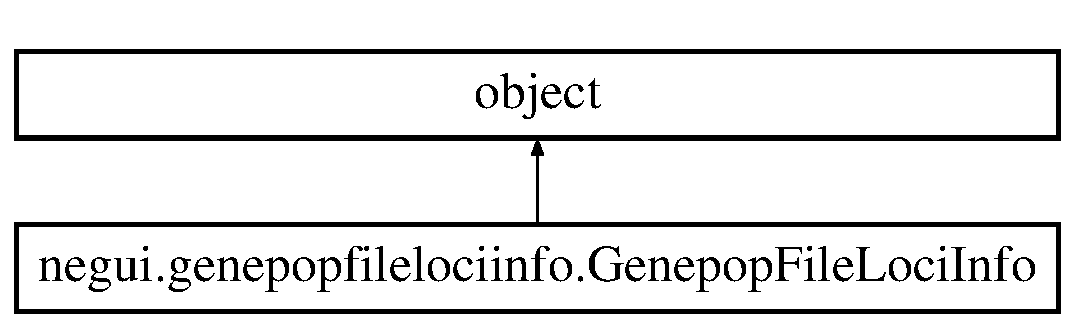
\includegraphics[height=2.000000cm]{classnegui_1_1genepopfilelociinfo_1_1GenepopFileLociInfo}
\end{center}
\end{figure}
\subsection*{Public Member Functions}
\begin{DoxyCompactItemize}
\item 
def \hyperlink{classnegui_1_1genepopfilelociinfo_1_1GenepopFileLociInfo_a28089049eada8659a3d8c5f35d194aac}{\+\_\+\+\_\+init\+\_\+\+\_\+} (self, o\+\_\+genepopfile, s\+\_\+population\+\_\+subsample\+\_\+tag=None, s\+\_\+individual\+\_\+subsample\+\_\+tag=None, s\+\_\+loci\+\_\+subsample\+\_\+tag=None)
\item 
def {\bfseries get\+Allele\+Frequencies} (self)\hypertarget{classnegui_1_1genepopfilelociinfo_1_1GenepopFileLociInfo_a58ebbff766dcdc78a0a12bf0cd1bbec6}{}\label{classnegui_1_1genepopfilelociinfo_1_1GenepopFileLociInfo_a58ebbff766dcdc78a0a12bf0cd1bbec6}

\item 
def {\bfseries get\+Heterozygosity} (self)\hypertarget{classnegui_1_1genepopfilelociinfo_1_1GenepopFileLociInfo_acaa07360c01954cc93dc595c2a0ff240}{}\label{classnegui_1_1genepopfilelociinfo_1_1GenepopFileLociInfo_acaa07360c01954cc93dc595c2a0ff240}

\item 
def {\bfseries population\+\_\+subsample\+\_\+name} (self)\hypertarget{classnegui_1_1genepopfilelociinfo_1_1GenepopFileLociInfo_a4bb83629fa1f6b9bb2a442eaa19bb09b}{}\label{classnegui_1_1genepopfilelociinfo_1_1GenepopFileLociInfo_a4bb83629fa1f6b9bb2a442eaa19bb09b}

\item 
def {\bfseries population\+\_\+subsample\+\_\+name} (self, s\+\_\+name)\hypertarget{classnegui_1_1genepopfilelociinfo_1_1GenepopFileLociInfo_a6ba9b9e9512ac3e9f6028f447aa64e80}{}\label{classnegui_1_1genepopfilelociinfo_1_1GenepopFileLociInfo_a6ba9b9e9512ac3e9f6028f447aa64e80}

\item 
def {\bfseries individual\+\_\+subsample\+\_\+name} (self)\hypertarget{classnegui_1_1genepopfilelociinfo_1_1GenepopFileLociInfo_af5fadee46f93aace5513738ed0f2ddb0}{}\label{classnegui_1_1genepopfilelociinfo_1_1GenepopFileLociInfo_af5fadee46f93aace5513738ed0f2ddb0}

\item 
def {\bfseries individual\+\_\+subsample\+\_\+name} (self, s\+\_\+name)\hypertarget{classnegui_1_1genepopfilelociinfo_1_1GenepopFileLociInfo_a503c6ae38a3435c6bbc6e37b51202c77}{}\label{classnegui_1_1genepopfilelociinfo_1_1GenepopFileLociInfo_a503c6ae38a3435c6bbc6e37b51202c77}

\item 
def {\bfseries loci\+\_\+subsample\+\_\+name} (self)\hypertarget{classnegui_1_1genepopfilelociinfo_1_1GenepopFileLociInfo_a8556fc2201edb72248b464ccd45f1ddc}{}\label{classnegui_1_1genepopfilelociinfo_1_1GenepopFileLociInfo_a8556fc2201edb72248b464ccd45f1ddc}

\item 
def {\bfseries loci\+\_\+subsample\+\_\+name} (self, s\+\_\+name)\hypertarget{classnegui_1_1genepopfilelociinfo_1_1GenepopFileLociInfo_afb8099ba82dee18eea5975a8c80fe83c}{}\label{classnegui_1_1genepopfilelociinfo_1_1GenepopFileLociInfo_afb8099ba82dee18eea5975a8c80fe83c}

\end{DoxyCompactItemize}


\subsection{Detailed Description}


Definition at line 27 of file genepopfilelociinfo.\+py.



\subsection{Constructor \& Destructor Documentation}
\index{negui\+::genepopfilelociinfo\+::\+Genepop\+File\+Loci\+Info@{negui\+::genepopfilelociinfo\+::\+Genepop\+File\+Loci\+Info}!\+\_\+\+\_\+init\+\_\+\+\_\+@{\+\_\+\+\_\+init\+\_\+\+\_\+}}
\index{\+\_\+\+\_\+init\+\_\+\+\_\+@{\+\_\+\+\_\+init\+\_\+\+\_\+}!negui\+::genepopfilelociinfo\+::\+Genepop\+File\+Loci\+Info@{negui\+::genepopfilelociinfo\+::\+Genepop\+File\+Loci\+Info}}
\subsubsection[{\texorpdfstring{\+\_\+\+\_\+init\+\_\+\+\_\+(self, o\+\_\+genepopfile, s\+\_\+population\+\_\+subsample\+\_\+tag=\+None, s\+\_\+individual\+\_\+subsample\+\_\+tag=\+None, s\+\_\+loci\+\_\+subsample\+\_\+tag=\+None)}{__init__(self, o_genepopfile, s_population_subsample_tag=None, s_individual_subsample_tag=None, s_loci_subsample_tag=None)}}]{\setlength{\rightskip}{0pt plus 5cm}def negui.\+genepopfilelociinfo.\+Genepop\+File\+Loci\+Info.\+\_\+\+\_\+init\+\_\+\+\_\+ (
\begin{DoxyParamCaption}
\item[{}]{self, }
\item[{}]{o\+\_\+genepopfile, }
\item[{}]{s\+\_\+population\+\_\+subsample\+\_\+tag = {\ttfamily None}, }
\item[{}]{s\+\_\+individual\+\_\+subsample\+\_\+tag = {\ttfamily None}, }
\item[{}]{s\+\_\+loci\+\_\+subsample\+\_\+tag = {\ttfamily None}}
\end{DoxyParamCaption}
)}\hypertarget{classnegui_1_1genepopfilelociinfo_1_1GenepopFileLociInfo_a28089049eada8659a3d8c5f35d194aac}{}\label{classnegui_1_1genepopfilelociinfo_1_1GenepopFileLociInfo_a28089049eada8659a3d8c5f35d194aac}
\begin{DoxyVerb}param o_genepopfile, a GenepopFileManager object
param s_population_subsample_tag, string giving the
      tag for a subsampling of the pops (pop sections)
      in the gnepop file managed by the GenepopFileManager
      object. If None, all pop sections are included.
param s_individual_subsample_tag, string giving the
      tag for a subsampling of the individuals in the
      included pops in the genepop file managed by the 
      GenepopFileManager object. If None, all individuals
      are included in each included pop section.
      all pop sections are included.
param s_individual_subsample_tag, string giving the
      tag for a subsampling of the loci in the
      included pops in the genepop file managed by the 
      GenepopFileManager object. If None, all individuals
      are included in each included pop section.
      all pop sections are included.
\end{DoxyVerb}
 

Definition at line 32 of file genepopfilelociinfo.\+py.


\begin{DoxyCode}
32                             s\_loci\_subsample\_tag=\textcolor{keywordtype}{None} ):
33 
34         \textcolor{stringliteral}{'''}
35 \textcolor{stringliteral}{        param o\_genepopfile, a GenepopFileManager object}
36 \textcolor{stringliteral}{        param s\_population\_subsample\_tag, string giving the}
37 \textcolor{stringliteral}{              tag for a subsampling of the pops (pop sections)}
38 \textcolor{stringliteral}{              in the gnepop file managed by the GenepopFileManager}
39 \textcolor{stringliteral}{              object. If None, all pop sections are included.}
40 \textcolor{stringliteral}{        param s\_individual\_subsample\_tag, string giving the}
41 \textcolor{stringliteral}{              tag for a subsampling of the individuals in the}
42 \textcolor{stringliteral}{              included pops in the genepop file managed by the }
43 \textcolor{stringliteral}{              GenepopFileManager object. If None, all individuals}
44 \textcolor{stringliteral}{              are included in each included pop section.}
45 \textcolor{stringliteral}{              all pop sections are included.}
46 \textcolor{stringliteral}{        param s\_individual\_subsample\_tag, string giving the}
47 \textcolor{stringliteral}{              tag for a subsampling of the loci in the}
48 \textcolor{stringliteral}{              included pops in the genepop file managed by the }
49 \textcolor{stringliteral}{              GenepopFileManager object. If None, all individuals}
50 \textcolor{stringliteral}{              are included in each included pop section.}
51 \textcolor{stringliteral}{              all pop sections are included.}
52 \textcolor{stringliteral}{        '''}
53 
54         self.\hyperlink{classnegui_1_1genepopfilelociinfo_1_1GenepopFileLociInfo_a11adb337e651f0218f32c66062f3eb9a}{\_\_genepop\_file}=o\_genepopfile
55         self.\hyperlink{classnegui_1_1genepopfilelociinfo_1_1GenepopFileLociInfo_a966eba4c51d001cee90f59914911334f}{\_\_pop\_subsample}=s\_population\_subsample\_tag
56         self.\hyperlink{classnegui_1_1genepopfilelociinfo_1_1GenepopFileLociInfo_abc390fd8a9530ccdf44595fc2e828e69}{\_\_indiv\_subsample}=s\_individual\_subsample\_tag
57         self.\hyperlink{classnegui_1_1genepopfilelociinfo_1_1GenepopFileLociInfo_a90e54c1c2cf515a05f76d5f10b8730d8}{\_\_loci\_subsample}=s\_loci\_subsample\_tag
58         
59         \textcolor{keywordflow}{return}
\end{DoxyCode}


The documentation for this class was generated from the following file\+:\begin{DoxyCompactItemize}
\item 
genepopfilelociinfo.\+py\end{DoxyCompactItemize}

\hypertarget{classnegui_1_1genepopfilemanager_1_1GenepopFileManager}{}\section{negui.\+genepopfilemanager.\+Genepop\+File\+Manager Class Reference}
\label{classnegui_1_1genepopfilemanager_1_1GenepopFileManager}\index{negui.\+genepopfilemanager.\+Genepop\+File\+Manager@{negui.\+genepopfilemanager.\+Genepop\+File\+Manager}}
Inheritance diagram for negui.\+genepopfilemanager.\+Genepop\+File\+Manager\+:\begin{figure}[H]
\begin{center}
\leavevmode
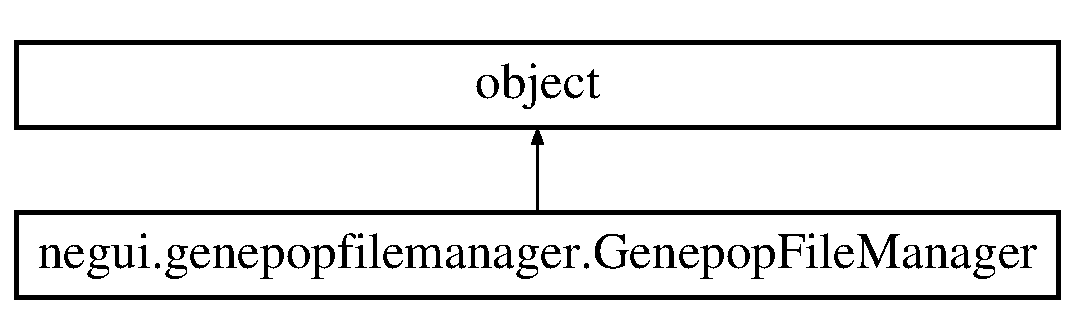
\includegraphics[height=2.000000cm]{classnegui_1_1genepopfilemanager_1_1GenepopFileManager}
\end{center}
\end{figure}
\subsection*{Public Member Functions}
\begin{DoxyCompactItemize}
\item 
def {\bfseries \+\_\+\+\_\+init\+\_\+\+\_\+} (self, s\+\_\+filename)\hypertarget{classnegui_1_1genepopfilemanager_1_1GenepopFileManager_a8563b3299666d02d45c9acd64f450c51}{}\label{classnegui_1_1genepopfilemanager_1_1GenepopFileManager_a8563b3299666d02d45c9acd64f450c51}

\item 
def {\bfseries write\+Gene\+Pop\+File} (self, s\+\_\+newfilename, s\+\_\+pop\+\_\+subsample\+\_\+tag=None, s\+\_\+indiv\+\_\+subsample\+\_\+tag=None, s\+\_\+loci\+\_\+subsample\+\_\+tag=None, i\+\_\+min\+\_\+pop\+\_\+size=0)\hypertarget{classnegui_1_1genepopfilemanager_1_1GenepopFileManager_a7390cad5840454284e816679a87d84df}{}\label{classnegui_1_1genepopfilemanager_1_1GenepopFileManager_a7390cad5840454284e816679a87d84df}

\item 
def {\bfseries print\+Gene\+Pop\+File} (self, s\+\_\+pop\+\_\+subsample\+\_\+tag=None, s\+\_\+indiv\+\_\+subsample\+\_\+tag=None, s\+\_\+loci\+\_\+subsample\+\_\+tag=None, i\+\_\+min\+\_\+pop\+\_\+size=0)\hypertarget{classnegui_1_1genepopfilemanager_1_1GenepopFileManager_a35aa30c43ab4a5e7762bf8c722314727}{}\label{classnegui_1_1genepopfilemanager_1_1GenepopFileManager_a35aa30c43ab4a5e7762bf8c722314727}

\item 
def {\bfseries get\+List\+Individual\+Numbers} (self, i\+\_\+pop\+\_\+number=1, s\+\_\+indiv\+\_\+subsample\+\_\+tag=None)\hypertarget{classnegui_1_1genepopfilemanager_1_1GenepopFileManager_a652029f0a6e0668e0b75c9683dae0ffd}{}\label{classnegui_1_1genepopfilemanager_1_1GenepopFileManager_a652029f0a6e0668e0b75c9683dae0ffd}

\item 
def \hyperlink{classnegui_1_1genepopfilemanager_1_1GenepopFileManager_a4334a9164415aa05de38ac7b31d59e40}{subsample\+Loci\+By\+Range\+And\+Max} (self, i\+\_\+min\+\_\+loci\+\_\+position, i\+\_\+max\+\_\+loci\+\_\+position, s\+\_\+loci\+\_\+subsample\+\_\+tag, i\+\_\+max\+\_\+total\+\_\+loci=None, b\+\_\+truncate\+\_\+max\+\_\+to\+\_\+total=True)
\item 
def \hyperlink{classnegui_1_1genepopfilemanager_1_1GenepopFileManager_af1dae6f9128c3c19ac204f518e838df1}{subsample\+Loci\+By\+Range\+And\+Proportion} (self, i\+\_\+min\+\_\+loci\+\_\+position, i\+\_\+max\+\_\+loci\+\_\+position, s\+\_\+loci\+\_\+subsample\+\_\+tag, f\+\_\+proportion\+\_\+of\+\_\+total\+\_\+loci, b\+\_\+truncate\+\_\+max\+\_\+to\+\_\+total=True)
\item 
def {\bfseries get\+List\+Individuals} (self, i\+\_\+pop\+\_\+number=1, s\+\_\+indiv\+\_\+subsample\+\_\+tag=None)\hypertarget{classnegui_1_1genepopfilemanager_1_1GenepopFileManager_aa6993dde24163002aeae55005437711d}{}\label{classnegui_1_1genepopfilemanager_1_1GenepopFileManager_aa6993dde24163002aeae55005437711d}

\item 
def {\bfseries get\+List\+Population\+Numbers} (self, s\+\_\+pop\+\_\+subsample\+\_\+tag=None)\hypertarget{classnegui_1_1genepopfilemanager_1_1GenepopFileManager_aa14e4cc93f6128be65081e2915969328}{}\label{classnegui_1_1genepopfilemanager_1_1GenepopFileManager_aa14e4cc93f6128be65081e2915969328}

\item 
def {\bfseries get\+List\+Empty\+Population\+Numbers} (self, s\+\_\+pop\+\_\+subsample\+\_\+tag=None, s\+\_\+indiv\+\_\+subsample\+\_\+tag=None)\hypertarget{classnegui_1_1genepopfilemanager_1_1GenepopFileManager_a05c943d32cf60349e9430ab9bd53e7d2}{}\label{classnegui_1_1genepopfilemanager_1_1GenepopFileManager_a05c943d32cf60349e9430ab9bd53e7d2}

\item 
def \hyperlink{classnegui_1_1genepopfilemanager_1_1GenepopFileManager_a5c85ac4838fd6919be1c408bcd39f54e}{subsample\+Individuals\+Randomly\+By\+Proportion} (self, f\+\_\+proportion\+\_\+to\+\_\+sample, s\+\_\+subsample\+\_\+tag)
\item 
def \hyperlink{classnegui_1_1genepopfilemanager_1_1GenepopFileManager_affaeb9457d84736dc1f289d600808f56}{subsample\+N\+Individuals\+Randomly\+From\+Each\+Pop} (self, i\+\_\+n, s\+\_\+subsample\+\_\+tag)
\item 
def {\bfseries subsample\+Loci\+By\+Name} (self, ls\+\_\+loci\+\_\+names, s\+\_\+subsample\+\_\+tag)\hypertarget{classnegui_1_1genepopfilemanager_1_1GenepopFileManager_afa08aba8e7a78951a6c0583aac52c9af}{}\label{classnegui_1_1genepopfilemanager_1_1GenepopFileManager_afa08aba8e7a78951a6c0583aac52c9af}

\item 
def {\bfseries subsample\+Individuals\+Minus\+Random\+N\+From\+Each\+Pop} (self, i\+\_\+n\+\_\+remove, s\+\_\+subsample\+\_\+tag)\hypertarget{classnegui_1_1genepopfilemanager_1_1GenepopFileManager_a97b12689980e0d6ce31c5882af1fd4e3}{}\label{classnegui_1_1genepopfilemanager_1_1GenepopFileManager_a97b12689980e0d6ce31c5882af1fd4e3}

\item 
def \hyperlink{classnegui_1_1genepopfilemanager_1_1GenepopFileManager_afb85a943b15c9a259510cc7f61b085b3}{subsample\+Individuals\+Leave\+Nth\+Out\+From\+Pop} (self, i\+\_\+n, i\+\_\+pop\+\_\+number, s\+\_\+indiv\+\_\+subsample\+\_\+tag)
\item 
def \hyperlink{classnegui_1_1genepopfilemanager_1_1GenepopFileManager_a361b30c9f9533b8610b3f587dc2677ea}{subsample\+Individuals\+By\+Id\+Criteria} (self, o\+\_\+genepop\+\_\+indiv\+\_\+id\+\_\+fields, o\+\_\+genepop\+\_\+indiv\+\_\+criteria, s\+\_\+subsample\+\_\+tag, i\+\_\+min\+\_\+pop\+\_\+sample\+\_\+size=None, i\+\_\+max\+\_\+pop\+\_\+sample\+\_\+size=None)
\item 
def \hyperlink{classnegui_1_1genepopfilemanager_1_1GenepopFileManager_abc486d49a3634caa7a64cd19cb6ff945}{subsample\+Individuals\+By\+Number\+List} (self, dli\+\_\+individual\+\_\+numbers, s\+\_\+subsample)
\item 
def \hyperlink{classnegui_1_1genepopfilemanager_1_1GenepopFileManager_afdad8528d7b19a8b2eeca447bb95a5a0}{subsample\+Individuals\+By\+Pop\+Size} (self, i\+\_\+min\+\_\+pop\+\_\+size, i\+\_\+max\+\_\+pop\+\_\+size, s\+\_\+subsample)
\item 
def \hyperlink{classnegui_1_1genepopfilemanager_1_1GenepopFileManager_a7e33739c660032e607db1066c4edd1f8}{get\+List\+Tuples\+Values\+Indiv\+Id\+Fields} (self, o\+\_\+genepop\+\_\+indiv\+\_\+id\+\_\+fields, ls\+\_\+field\+\_\+names)
\item 
def {\bfseries subsample\+Populations\+By\+List} (self, li\+\_\+pop\+\_\+numbers, s\+\_\+subsample\+\_\+tag)\hypertarget{classnegui_1_1genepopfilemanager_1_1GenepopFileManager_aab1109500d95ec010b4c39f198bb41c9}{}\label{classnegui_1_1genepopfilemanager_1_1GenepopFileManager_aab1109500d95ec010b4c39f198bb41c9}

\item 
def \hyperlink{classnegui_1_1genepopfilemanager_1_1GenepopFileManager_aca743749002b9828cd66730e42db4387}{get\+Individual\+Counts} (self, s\+\_\+pop\+\_\+subsample\+\_\+tag=None, s\+\_\+indiv\+\_\+subsample\+\_\+tag=None)
\item 
def \hyperlink{classnegui_1_1genepopfilemanager_1_1GenepopFileManager_a05e723069f5129b21a4d017c2a5317b0}{get\+Individual\+Count} (self, i\+\_\+pop\+\_\+number, s\+\_\+indiv\+\_\+subsample\+\_\+tag=None)
\item 
def {\bfseries combine\+Individual\+Subsamples} (self, ls\+\_\+subsample\+\_\+tags, s\+\_\+tag\+\_\+for\+\_\+combined\+\_\+subsample)\hypertarget{classnegui_1_1genepopfilemanager_1_1GenepopFileManager_a3f62c4250a0aa8a9b810424d0f62c068}{}\label{classnegui_1_1genepopfilemanager_1_1GenepopFileManager_a3f62c4250a0aa8a9b810424d0f62c068}

\item 
def {\bfseries remove\+Individual\+Subsamples} (ls\+\_\+subsample\+\_\+tags)\hypertarget{classnegui_1_1genepopfilemanager_1_1GenepopFileManager_ae0f452a29252cdd75393effc2baa9299}{}\label{classnegui_1_1genepopfilemanager_1_1GenepopFileManager_ae0f452a29252cdd75393effc2baa9299}

\item 
def {\bfseries pop\+\_\+total} (self)\hypertarget{classnegui_1_1genepopfilemanager_1_1GenepopFileManager_afeefa4552274231bedce1fc6b8c0532d}{}\label{classnegui_1_1genepopfilemanager_1_1GenepopFileManager_afeefa4552274231bedce1fc6b8c0532d}

\item 
def \hyperlink{classnegui_1_1genepopfilemanager_1_1GenepopFileManager_ac3210c8f51c32e9e99e34703afb402d0}{population\+\_\+subsample\+\_\+tags} (self)
\item 
def \hyperlink{classnegui_1_1genepopfilemanager_1_1GenepopFileManager_ae77bd8c465db4d95839db838c236f4cd}{indiv\+\_\+subsample\+\_\+tags} (self)
\item 
def \hyperlink{classnegui_1_1genepopfilemanager_1_1GenepopFileManager_a9818ed890508a24026ea37fa734c898e}{loci\+\_\+subsample\+\_\+tags} (self)
\item 
def {\bfseries original\+\_\+file\+\_\+name} (self)\hypertarget{classnegui_1_1genepopfilemanager_1_1GenepopFileManager_a8145be8434d89aa7011831f6a6ca19a3}{}\label{classnegui_1_1genepopfilemanager_1_1GenepopFileManager_a8145be8434d89aa7011831f6a6ca19a3}

\item 
def \hyperlink{classnegui_1_1genepopfilemanager_1_1GenepopFileManager_abec8e261bad014e6488162ec43e63ef7}{original\+\_\+file\+\_\+name} (self, s\+\_\+filename)
\end{DoxyCompactItemize}
\subsection*{Static Public Attributes}
\begin{DoxyCompactItemize}
\item 
int {\bfseries K\+E\+Y\+\_\+\+F\+I\+R\+S\+T\+\_\+\+I\+N\+D\+I\+V\+\_\+\+N\+U\+M\+B\+ER} = 1\hypertarget{classnegui_1_1genepopfilemanager_1_1GenepopFileManager_a1f8674fb73d5d2ec44967108406b39c9}{}\label{classnegui_1_1genepopfilemanager_1_1GenepopFileManager_a1f8674fb73d5d2ec44967108406b39c9}

\item 
int {\bfseries K\+E\+Y\+\_\+\+F\+I\+R\+S\+T\+\_\+\+L\+I\+N\+E\+\_\+\+I\+N\+D\+I\+V\+\_\+\+E\+N\+T\+RY} = 1\hypertarget{classnegui_1_1genepopfilemanager_1_1GenepopFileManager_aaec5489b8872faeaf8830e5aea2095bf}{}\label{classnegui_1_1genepopfilemanager_1_1GenepopFileManager_aaec5489b8872faeaf8830e5aea2095bf}

\item 
int {\bfseries K\+E\+Y\+\_\+\+P\+O\+P\+\_\+\+E\+N\+T\+RY} = 0\hypertarget{classnegui_1_1genepopfilemanager_1_1GenepopFileManager_ac4f9b53217279103e40c65697d279616}{}\label{classnegui_1_1genepopfilemanager_1_1GenepopFileManager_ac4f9b53217279103e40c65697d279616}

\end{DoxyCompactItemize}


\subsection{Detailed Description}
\begin{DoxyVerb}wraps 2 dictionaries, one for header and loci byte addresses, the other for 
        byte addresses of "pop" lines and individual addresses.  The header dict 
        has one level, the pop dict  has 3 levels:
        outer key: for the pop dict, pop number: 1,2..., for header/loci simply the line number
        middle key: pop dict only,   item number: 0,1,2
            for the pop dictionsary the first "pop" line itself is the zeroth item
            and for pop 1,2,..., the entry "pop"
        innermost key:  item-line number, 0,1,2...
            this key needed because genepop allows multi line entries for
            a single individual
    value: byte address of the first byte of the line

    example, if (as most often) the individual entry takes up only one line, 
    to find the entry for the 2nd indiv at pop 2, point the file pointer at 
    the byte address given by self.__byte_addresses[2][2][1], and execute a readline().  
    If this individual was on more than one line, say 2 lines, the entry would 8
    be given by concatenating the lines read at self.__byte_addresses[2][2][1] 
    and self.__byte_addresses[2][2][2]

    Note that we aim to parse the genepop file in accordance with the format described
    in http://genepop.curtin.edu.au/help_input.html#Input as accessed most recently
    on 2016_10_03.
\end{DoxyVerb}
\begin{DoxyVerb}These constants are added on 2016_10_03
and will be incorporated into new code
as reminders of the correct keys that
fetches the dictionary that holds byte addresse(s) 
(plural only if the id + loci are entered
on multiple lines) of the first indiv:
\end{DoxyVerb}
 

Definition at line 14 of file genepopfilemanager.\+py.



\subsection{Member Function Documentation}
\index{negui\+::genepopfilemanager\+::\+Genepop\+File\+Manager@{negui\+::genepopfilemanager\+::\+Genepop\+File\+Manager}!get\+Individual\+Count@{get\+Individual\+Count}}
\index{get\+Individual\+Count@{get\+Individual\+Count}!negui\+::genepopfilemanager\+::\+Genepop\+File\+Manager@{negui\+::genepopfilemanager\+::\+Genepop\+File\+Manager}}
\subsubsection[{\texorpdfstring{get\+Individual\+Count(self, i\+\_\+pop\+\_\+number, s\+\_\+indiv\+\_\+subsample\+\_\+tag=\+None)}{getIndividualCount(self, i_pop_number, s_indiv_subsample_tag=None)}}]{\setlength{\rightskip}{0pt plus 5cm}def negui.\+genepopfilemanager.\+Genepop\+File\+Manager.\+get\+Individual\+Count (
\begin{DoxyParamCaption}
\item[{}]{self, }
\item[{}]{i\+\_\+pop\+\_\+number, }
\item[{}]{s\+\_\+indiv\+\_\+subsample\+\_\+tag = {\ttfamily None}}
\end{DoxyParamCaption}
)}\hypertarget{classnegui_1_1genepopfilemanager_1_1GenepopFileManager_a05e723069f5129b21a4d017c2a5317b0}{}\label{classnegui_1_1genepopfilemanager_1_1GenepopFileManager_a05e723069f5129b21a4d017c2a5317b0}
\begin{DoxyVerb}Expects 1-based population number.
Returns the individual count for the ith of N populations, i=1,2,3...N
If s_indiv_subsample_tag is supplied, then the counts will
reflect those of the individuals in the ith population after
the sampling named by the tag.
\end{DoxyVerb}
 

Definition at line 1338 of file genepopfilemanager.\+py.


\begin{DoxyCode}
1338     \textcolor{keyword}{def }\hyperlink{classnegui_1_1genepopfilemanager_1_1GenepopFileManager_a05e723069f5129b21a4d017c2a5317b0}{getIndividualCount}( self, i\_pop\_number, s\_indiv\_subsample\_tag=None ):
1339         \textcolor{stringliteral}{'''}
1340 \textcolor{stringliteral}{        Expects 1-based population number.}
1341 \textcolor{stringliteral}{        Returns the individual count for the ith of N populations, i=1,2,3...N}
1342 \textcolor{stringliteral}{        If s\_indiv\_subsample\_tag is supplied, then the counts will}
1343 \textcolor{stringliteral}{        reflect those of the individuals in the ith population after}
1344 \textcolor{stringliteral}{        the sampling named by the tag.}
1345 \textcolor{stringliteral}{        '''}
1346 
1347         i\_total\_pops\_in\_file=self.\hyperlink{classnegui_1_1genepopfilemanager_1_1GenepopFileManager_a51f6dcbd17c80f8e61114b11283b655f}{\_\_get\_count\_populations}()  
1348 
1349         \textcolor{keywordflow}{if} i\_pop\_number < 1 \textcolor{keywordflow}{or} i\_pop\_number > i\_total\_pops\_in\_file:
1350 
1351             s\_msg=\textcolor{stringliteral}{"In GenepopFileManager instance, def getIndividualCount, "} \(\backslash\)
1352                     + \textcolor{stringliteral}{"invalid population number for file with total populations, "} \(\backslash\)
1353                     + str( i\_total\_pops\_in\_file ) \(\backslash\)
1354                     + \textcolor{stringliteral}{".  Pop number requested: "} + str( i\_pop\_number ) + \textcolor{stringliteral}{"."}
1355 
1356             \textcolor{keywordflow}{raise} Exception( s\_msg )
1357 
1358         \textcolor{comment}{#end if  invalid population number}
1359 
1360         li\_counts=\textcolor{keywordtype}{None}
1361 
1362         li\_counts=self.\hyperlink{classnegui_1_1genepopfilemanager_1_1GenepopFileManager_a8efe11151549d7da2bc024f836491af4}{\_\_get\_count\_indiv\_per\_pop}( s\_indiv\_subsample\_tag )
1363         \textcolor{comment}{#end if we get counts from subsample}
1364 
1365         \textcolor{keywordflow}{return} li\_counts[ i\_pop\_number - 1 ]
\end{DoxyCode}
\index{negui\+::genepopfilemanager\+::\+Genepop\+File\+Manager@{negui\+::genepopfilemanager\+::\+Genepop\+File\+Manager}!get\+Individual\+Counts@{get\+Individual\+Counts}}
\index{get\+Individual\+Counts@{get\+Individual\+Counts}!negui\+::genepopfilemanager\+::\+Genepop\+File\+Manager@{negui\+::genepopfilemanager\+::\+Genepop\+File\+Manager}}
\subsubsection[{\texorpdfstring{get\+Individual\+Counts(self, s\+\_\+pop\+\_\+subsample\+\_\+tag=\+None, s\+\_\+indiv\+\_\+subsample\+\_\+tag=\+None)}{getIndividualCounts(self, s_pop_subsample_tag=None, s_indiv_subsample_tag=None)}}]{\setlength{\rightskip}{0pt plus 5cm}def negui.\+genepopfilemanager.\+Genepop\+File\+Manager.\+get\+Individual\+Counts (
\begin{DoxyParamCaption}
\item[{}]{self, }
\item[{}]{s\+\_\+pop\+\_\+subsample\+\_\+tag = {\ttfamily None}, }
\item[{}]{s\+\_\+indiv\+\_\+subsample\+\_\+tag = {\ttfamily None}}
\end{DoxyParamCaption}
)}\hypertarget{classnegui_1_1genepopfilemanager_1_1GenepopFileManager_aca743749002b9828cd66730e42db4387}{}\label{classnegui_1_1genepopfilemanager_1_1GenepopFileManager_aca743749002b9828cd66730e42db4387}
\begin{DoxyVerb}Returns a list of individual counts (total individuals) for each of N populations
numbered 1,2,3,...N, representing the "pop" entries in order in the genepop file
to which this GenepopFileManager instance corresponds.

If s_pop_subsample_tag is not None, then the list will contain counts for each
population in some subset of the original N, as listed by population nunber 
list associated with the population subsample tag.

If s_indiv_subsample_tag is not None, then the counts will be for the individuals
in each pop as subsampled.
\end{DoxyVerb}
 

Definition at line 1316 of file genepopfilemanager.\+py.


\begin{DoxyCode}
1316     \textcolor{keyword}{def }\hyperlink{classnegui_1_1genepopfilemanager_1_1GenepopFileManager_aca743749002b9828cd66730e42db4387}{getIndividualCounts}( self, s\_pop\_subsample\_tag=None, s\_indiv\_subsample\_tag=None 
      ):
1317 
1318         \textcolor{stringliteral}{'''}
1319 \textcolor{stringliteral}{        Returns a list of individual counts (total individuals) for each of N populations}
1320 \textcolor{stringliteral}{        numbered 1,2,3,...N, representing the "pop" entries in order in the genepop file}
1321 \textcolor{stringliteral}{        to which this GenepopFileManager instance corresponds.}
1322 \textcolor{stringliteral}{}
1323 \textcolor{stringliteral}{        If s\_pop\_subsample\_tag is not None, then the list will contain counts for each}
1324 \textcolor{stringliteral}{        population in some subset of the original N, as listed by population nunber }
1325 \textcolor{stringliteral}{        list associated with the population subsample tag.}
1326 \textcolor{stringliteral}{}
1327 \textcolor{stringliteral}{        If s\_indiv\_subsample\_tag is not None, then the counts will be for the individuals}
1328 \textcolor{stringliteral}{        in each pop as subsampled.}
1329 \textcolor{stringliteral}{        '''}
1330         li\_counts=\textcolor{keywordtype}{None}
1331 
1332         li\_counts=self.\hyperlink{classnegui_1_1genepopfilemanager_1_1GenepopFileManager_a8efe11151549d7da2bc024f836491af4}{\_\_get\_count\_indiv\_per\_pop}( s\_indiv\_subsample\_tag, 
      s\_pop\_subsample\_tag ) 
1333 
1334         \textcolor{keywordflow}{return} li\_counts
1335 
\end{DoxyCode}
\index{negui\+::genepopfilemanager\+::\+Genepop\+File\+Manager@{negui\+::genepopfilemanager\+::\+Genepop\+File\+Manager}!get\+List\+Tuples\+Values\+Indiv\+Id\+Fields@{get\+List\+Tuples\+Values\+Indiv\+Id\+Fields}}
\index{get\+List\+Tuples\+Values\+Indiv\+Id\+Fields@{get\+List\+Tuples\+Values\+Indiv\+Id\+Fields}!negui\+::genepopfilemanager\+::\+Genepop\+File\+Manager@{negui\+::genepopfilemanager\+::\+Genepop\+File\+Manager}}
\subsubsection[{\texorpdfstring{get\+List\+Tuples\+Values\+Indiv\+Id\+Fields(self, o\+\_\+genepop\+\_\+indiv\+\_\+id\+\_\+fields, ls\+\_\+field\+\_\+names)}{getListTuplesValuesIndivIdFields(self, o_genepop_indiv_id_fields, ls_field_names)}}]{\setlength{\rightskip}{0pt plus 5cm}def negui.\+genepopfilemanager.\+Genepop\+File\+Manager.\+get\+List\+Tuples\+Values\+Indiv\+Id\+Fields (
\begin{DoxyParamCaption}
\item[{}]{self, }
\item[{}]{o\+\_\+genepop\+\_\+indiv\+\_\+id\+\_\+fields, }
\item[{}]{ls\+\_\+field\+\_\+names}
\end{DoxyParamCaption}
)}\hypertarget{classnegui_1_1genepopfilemanager_1_1GenepopFileManager_a7e33739c660032e607db1066c4edd1f8}{}\label{classnegui_1_1genepopfilemanager_1_1GenepopFileManager_a7e33739c660032e607db1066c4edd1f8}
\begin{DoxyVerb}Need a method to get the set (i.e. unique tuple) of 
existing values for seom combo of ID fields 
(may be only one field).  This would 
be step one in a generalized implementation of Tiago's 
sampleIndivsRelated.py code. Once we have the set of tuples 
giving existing values, we can then use criteria matching 
to subsample pops by testing each indiv for (a) matching 
field value(s), using def subsampleIndividualsByIdCriteria.  
Note that we can add criteria to the tests, for example, 
to add age==1 to a criteria that also requires a father==i 
and mother==j match, each i and j supplied by this def.

arg o_genepop_indiv_id_fields, an instance of GenepopIndivIdFields
arg ls_field_names, a list of strings that ell which of the field names
in o_genepop_indiv_id_fields gives the fields to group to find
all uniq value combos.

As of 2016_09_08, this not yet implemented
\end{DoxyVerb}
 

Definition at line 1242 of file genepopfilemanager.\+py.


\begin{DoxyCode}
1242                             ls\_field\_names ):
1243 
1244         \textcolor{stringliteral}{'''}
1245 \textcolor{stringliteral}{        Need a method to get the set (i.e. unique tuple) of }
1246 \textcolor{stringliteral}{        existing values for seom combo of ID fields }
1247 \textcolor{stringliteral}{        (may be only one field).  This would }
1248 \textcolor{stringliteral}{        be step one in a generalized implementation of Tiago's }
1249 \textcolor{stringliteral}{        sampleIndivsRelated.py code. Once we have the set of tuples }
1250 \textcolor{stringliteral}{        giving existing values, we can then use criteria matching }
1251 \textcolor{stringliteral}{        to subsample pops by testing each indiv for (a) matching }
1252 \textcolor{stringliteral}{        field value(s), using def subsampleIndividualsByIdCriteria.  }
1253 \textcolor{stringliteral}{        Note that we can add criteria to the tests, for example, }
1254 \textcolor{stringliteral}{        to add age==1 to a criteria that also requires a father==i }
1255 \textcolor{stringliteral}{        and mother==j match, each i and j supplied by this def.}
1256 \textcolor{stringliteral}{}
1257 \textcolor{stringliteral}{        arg o\_genepop\_indiv\_id\_fields, an instance of GenepopIndivIdFields}
1258 \textcolor{stringliteral}{        arg ls\_field\_names, a list of strings that ell which of the field names}
1259 \textcolor{stringliteral}{                in o\_genepop\_indiv\_id\_fields gives the fields to group to find}
1260 \textcolor{stringliteral}{                all uniq value combos.}
1261 \textcolor{stringliteral}{}
1262 \textcolor{stringliteral}{        As of 2016\_09\_08, this not yet implemented}
1263 \textcolor{stringliteral}{        '''}
1264 
1265         li\_pop\_numbers=self.\hyperlink{classnegui_1_1genepopfilemanager_1_1GenepopFileManager_a0cd3178624c652968b4d319f12e5df6e}{\_\_get\_pop\_list}() 
1266         set\_tuples\_values=set()
1267 
1268         \textcolor{keywordflow}{for} i\_pop\_number \textcolor{keywordflow}{in} li\_pop\_numbers:
1269             ls\_indiv\_ids\_this\_pop=self.\hyperlink{classnegui_1_1genepopfilemanager_1_1GenepopFileManager_aa6993dde24163002aeae55005437711d}{getListIndividuals}( i\_pop\_number=i\_pop\_number )
1270 
1271             \textcolor{keywordflow}{for} s\_id \textcolor{keywordflow}{in} ls\_indiv\_ids\_this\_pop:
1272 
1273                 o\_genepop\_id\_vals=GenepopIndivIdVals( s\_id, o\_genepop\_indiv\_id\_fields )
1274 
1275                 tv\_vals\_this\_id=tuple() 
1276 
1277                 \textcolor{keywordflow}{for} s\_field\_name \textcolor{keywordflow}{in} ls\_field\_names:
1278                     v\_val\_this\_field=o\_genepop\_id\_vals.getVal( s\_field\_name )
1279                     tv\_vals\_this\_id += ( v\_val, )
1280                 \textcolor{comment}{#end for each field, add to tuple}
1281 
1282                 set\_tuples\_values.union( \{ tv\_vals\_this\_id \} )
1283 
1284             \textcolor{comment}{#end for indiv id in this pop}
1285         \textcolor{comment}{#end for each pop in file}
1286 
1287         \textcolor{keywordflow}{return} list( set\_tuples\_values )
1288 
\end{DoxyCode}
\index{negui\+::genepopfilemanager\+::\+Genepop\+File\+Manager@{negui\+::genepopfilemanager\+::\+Genepop\+File\+Manager}!indiv\+\_\+subsample\+\_\+tags@{indiv\+\_\+subsample\+\_\+tags}}
\index{indiv\+\_\+subsample\+\_\+tags@{indiv\+\_\+subsample\+\_\+tags}!negui\+::genepopfilemanager\+::\+Genepop\+File\+Manager@{negui\+::genepopfilemanager\+::\+Genepop\+File\+Manager}}
\subsubsection[{\texorpdfstring{indiv\+\_\+subsample\+\_\+tags(self)}{indiv_subsample_tags(self)}}]{\setlength{\rightskip}{0pt plus 5cm}def negui.\+genepopfilemanager.\+Genepop\+File\+Manager.\+indiv\+\_\+subsample\+\_\+tags (
\begin{DoxyParamCaption}
\item[{}]{self}
\end{DoxyParamCaption}
)}\hypertarget{classnegui_1_1genepopfilemanager_1_1GenepopFileManager_ae77bd8c465db4d95839db838c236f4cd}{}\label{classnegui_1_1genepopfilemanager_1_1GenepopFileManager_ae77bd8c465db4d95839db838c236f4cd}
\begin{DoxyVerb}so user can iterate over subsamples,
we return a list of their tags:
\end{DoxyVerb}
 

Definition at line 1408 of file genepopfilemanager.\+py.


\begin{DoxyCode}
1408     \textcolor{keyword}{def }\hyperlink{classnegui_1_1genepopfilemanager_1_1GenepopFileManager_ae77bd8c465db4d95839db838c236f4cd}{indiv\_subsample\_tags}( self ):
1409         \textcolor{stringliteral}{'''}
1410 \textcolor{stringliteral}{        so user can iterate over subsamples,}
1411 \textcolor{stringliteral}{        we return a list of their tags:}
1412 \textcolor{stringliteral}{        '''}
1413         \textcolor{keywordflow}{return} [ s\_tag \textcolor{keywordflow}{for} s\_tag \textcolor{keywordflow}{in} self.\hyperlink{classnegui_1_1genepopfilemanager_1_1GenepopFileManager_a1e8379bcee4902ca9314ff53fcb71644}{\_\_indiv\_subsamples} ]
\end{DoxyCode}
\index{negui\+::genepopfilemanager\+::\+Genepop\+File\+Manager@{negui\+::genepopfilemanager\+::\+Genepop\+File\+Manager}!loci\+\_\+subsample\+\_\+tags@{loci\+\_\+subsample\+\_\+tags}}
\index{loci\+\_\+subsample\+\_\+tags@{loci\+\_\+subsample\+\_\+tags}!negui\+::genepopfilemanager\+::\+Genepop\+File\+Manager@{negui\+::genepopfilemanager\+::\+Genepop\+File\+Manager}}
\subsubsection[{\texorpdfstring{loci\+\_\+subsample\+\_\+tags(self)}{loci_subsample_tags(self)}}]{\setlength{\rightskip}{0pt plus 5cm}def negui.\+genepopfilemanager.\+Genepop\+File\+Manager.\+loci\+\_\+subsample\+\_\+tags (
\begin{DoxyParamCaption}
\item[{}]{self}
\end{DoxyParamCaption}
)}\hypertarget{classnegui_1_1genepopfilemanager_1_1GenepopFileManager_a9818ed890508a24026ea37fa734c898e}{}\label{classnegui_1_1genepopfilemanager_1_1GenepopFileManager_a9818ed890508a24026ea37fa734c898e}
\begin{DoxyVerb}so user can iterate over subsamples,
we return a list of their tags:
\end{DoxyVerb}
 

Definition at line 1417 of file genepopfilemanager.\+py.


\begin{DoxyCode}
1417     \textcolor{keyword}{def }\hyperlink{classnegui_1_1genepopfilemanager_1_1GenepopFileManager_a9818ed890508a24026ea37fa734c898e}{loci\_subsample\_tags}( self ):
1418         \textcolor{stringliteral}{'''}
1419 \textcolor{stringliteral}{        so user can iterate over subsamples,}
1420 \textcolor{stringliteral}{        we return a list of their tags:}
1421 \textcolor{stringliteral}{        '''}
1422         \textcolor{keywordflow}{return} [ s\_tag \textcolor{keywordflow}{for} s\_tag \textcolor{keywordflow}{in} self.\hyperlink{classnegui_1_1genepopfilemanager_1_1GenepopFileManager_af867ba70728e8a3aaf0097ddd6399e28}{\_\_loci\_subsamples} ]
\end{DoxyCode}
\index{negui\+::genepopfilemanager\+::\+Genepop\+File\+Manager@{negui\+::genepopfilemanager\+::\+Genepop\+File\+Manager}!original\+\_\+file\+\_\+name@{original\+\_\+file\+\_\+name}}
\index{original\+\_\+file\+\_\+name@{original\+\_\+file\+\_\+name}!negui\+::genepopfilemanager\+::\+Genepop\+File\+Manager@{negui\+::genepopfilemanager\+::\+Genepop\+File\+Manager}}
\subsubsection[{\texorpdfstring{original\+\_\+file\+\_\+name(self, s\+\_\+filename)}{original_file_name(self, s_filename)}}]{\setlength{\rightskip}{0pt plus 5cm}def negui.\+genepopfilemanager.\+Genepop\+File\+Manager.\+original\+\_\+file\+\_\+name (
\begin{DoxyParamCaption}
\item[{}]{self, }
\item[{}]{s\+\_\+filename}
\end{DoxyParamCaption}
)}\hypertarget{classnegui_1_1genepopfilemanager_1_1GenepopFileManager_abec8e261bad014e6488162ec43e63ef7}{}\label{classnegui_1_1genepopfilemanager_1_1GenepopFileManager_abec8e261bad014e6488162ec43e63ef7}
\begin{DoxyVerb}this setter essentially creates a new object
based on the genepop file with the filename 
given by param s_filename
\end{DoxyVerb}
 

Definition at line 1431 of file genepopfilemanager.\+py.


\begin{DoxyCode}
1431     \textcolor{keyword}{def }original\_file\_name( self, s\_filename ):
1432         \textcolor{stringliteral}{'''}
1433 \textcolor{stringliteral}{        this setter essentially creates a new object}
1434 \textcolor{stringliteral}{        based on the genepop file with the filename }
1435 \textcolor{stringliteral}{        given by param s\_filename}
1436 \textcolor{stringliteral}{        '''}
1437         self.\hyperlink{classnegui_1_1genepopfilemanager_1_1GenepopFileManager_a2f6cd645e29db938befdf961d0819777}{\_\_filename}=s\_filename
1438         self.\hyperlink{classnegui_1_1genepopfilemanager_1_1GenepopFileManager_a77a97fe40279f37b14f23c5e4180abc5}{\_\_setup\_addresses}( s\_filename )
1439         self.\hyperlink{classnegui_1_1genepopfilemanager_1_1GenepopFileManager_ab05c5daa99f1b294c019769b1e60ae20}{\_\_init\_subsamples}()
1440         \textcolor{keywordflow}{return}
\end{DoxyCode}
\index{negui\+::genepopfilemanager\+::\+Genepop\+File\+Manager@{negui\+::genepopfilemanager\+::\+Genepop\+File\+Manager}!population\+\_\+subsample\+\_\+tags@{population\+\_\+subsample\+\_\+tags}}
\index{population\+\_\+subsample\+\_\+tags@{population\+\_\+subsample\+\_\+tags}!negui\+::genepopfilemanager\+::\+Genepop\+File\+Manager@{negui\+::genepopfilemanager\+::\+Genepop\+File\+Manager}}
\subsubsection[{\texorpdfstring{population\+\_\+subsample\+\_\+tags(self)}{population_subsample_tags(self)}}]{\setlength{\rightskip}{0pt plus 5cm}def negui.\+genepopfilemanager.\+Genepop\+File\+Manager.\+population\+\_\+subsample\+\_\+tags (
\begin{DoxyParamCaption}
\item[{}]{self}
\end{DoxyParamCaption}
)}\hypertarget{classnegui_1_1genepopfilemanager_1_1GenepopFileManager_ac3210c8f51c32e9e99e34703afb402d0}{}\label{classnegui_1_1genepopfilemanager_1_1GenepopFileManager_ac3210c8f51c32e9e99e34703afb402d0}
\begin{DoxyVerb}so user can iterate over populations
as subsampled
\end{DoxyVerb}
 

Definition at line 1399 of file genepopfilemanager.\+py.


\begin{DoxyCode}
1399     \textcolor{keyword}{def }\hyperlink{classnegui_1_1genepopfilemanager_1_1GenepopFileManager_ac3210c8f51c32e9e99e34703afb402d0}{population\_subsample\_tags}( self ):
1400         \textcolor{stringliteral}{'''}
1401 \textcolor{stringliteral}{        so user can iterate over populations}
1402 \textcolor{stringliteral}{        as subsampled}
1403 \textcolor{stringliteral}{        '''}
1404         \textcolor{keywordflow}{return} [ s\_tag \textcolor{keywordflow}{for} s\_tag \textcolor{keywordflow}{in} self.\hyperlink{classnegui_1_1genepopfilemanager_1_1GenepopFileManager_a3a99a5030db49684ac320b1dc456c1fd}{\_\_pop\_subsamples} ]
\end{DoxyCode}
\index{negui\+::genepopfilemanager\+::\+Genepop\+File\+Manager@{negui\+::genepopfilemanager\+::\+Genepop\+File\+Manager}!subsample\+Individuals\+By\+Id\+Criteria@{subsample\+Individuals\+By\+Id\+Criteria}}
\index{subsample\+Individuals\+By\+Id\+Criteria@{subsample\+Individuals\+By\+Id\+Criteria}!negui\+::genepopfilemanager\+::\+Genepop\+File\+Manager@{negui\+::genepopfilemanager\+::\+Genepop\+File\+Manager}}
\subsubsection[{\texorpdfstring{subsample\+Individuals\+By\+Id\+Criteria(self, o\+\_\+genepop\+\_\+indiv\+\_\+id\+\_\+fields, o\+\_\+genepop\+\_\+indiv\+\_\+criteria, s\+\_\+subsample\+\_\+tag, i\+\_\+min\+\_\+pop\+\_\+sample\+\_\+size=\+None, i\+\_\+max\+\_\+pop\+\_\+sample\+\_\+size=\+None)}{subsampleIndividualsByIdCriteria(self, o_genepop_indiv_id_fields, o_genepop_indiv_criteria, s_subsample_tag, i_min_pop_sample_size=None, i_max_pop_sample_size=None)}}]{\setlength{\rightskip}{0pt plus 5cm}def negui.\+genepopfilemanager.\+Genepop\+File\+Manager.\+subsample\+Individuals\+By\+Id\+Criteria (
\begin{DoxyParamCaption}
\item[{}]{self, }
\item[{}]{o\+\_\+genepop\+\_\+indiv\+\_\+id\+\_\+fields, }
\item[{}]{o\+\_\+genepop\+\_\+indiv\+\_\+criteria, }
\item[{}]{s\+\_\+subsample\+\_\+tag, }
\item[{}]{i\+\_\+min\+\_\+pop\+\_\+sample\+\_\+size = {\ttfamily None}, }
\item[{}]{i\+\_\+max\+\_\+pop\+\_\+sample\+\_\+size = {\ttfamily None}}
\end{DoxyParamCaption}
)}\hypertarget{classnegui_1_1genepopfilemanager_1_1GenepopFileManager_a361b30c9f9533b8610b3f587dc2677ea}{}\label{classnegui_1_1genepopfilemanager_1_1GenepopFileManager_a361b30c9f9533b8610b3f587dc2677ea}
\begin{DoxyVerb}param o_genepop_indiv_id_fields, an instance of GenepopIndivIdFields

param o_genepop_indiv_criteria, a GenepopIndivCriteria instance,
    itself a list of GenepopIndivCriterion instances, with
    the ability to perform all criterion tests and return True or False

Assumes that the list of individual (ids)
from call to getListIndividuals gives ids
in the same order as they occur in the 
original genepop file.
\end{DoxyVerb}
 

Definition at line 1095 of file genepopfilemanager.\+py.


\begin{DoxyCode}
1095                                             i\_max\_pop\_sample\_size=\textcolor{keywordtype}{None} ):
1096         \textcolor{stringliteral}{'''}
1097 \textcolor{stringliteral}{        param o\_genepop\_indiv\_id\_fields, an instance of GenepopIndivIdFields}
1098 \textcolor{stringliteral}{}
1099 \textcolor{stringliteral}{        param o\_genepop\_indiv\_criteria, a GenepopIndivCriteria instance,}
1100 \textcolor{stringliteral}{            itself a list of GenepopIndivCriterion instances, with}
1101 \textcolor{stringliteral}{            the ability to perform all criterion tests and return True or False}
1102 \textcolor{stringliteral}{}
1103 \textcolor{stringliteral}{        Assumes that the list of individual (ids)}
1104 \textcolor{stringliteral}{        from call to getListIndividuals gives ids}
1105 \textcolor{stringliteral}{        in the same order as they occur in the }
1106 \textcolor{stringliteral}{        original genepop file.}
1107 \textcolor{stringliteral}{        '''}
1108         self.\hyperlink{classnegui_1_1genepopfilemanager_1_1GenepopFileManager_a1e8379bcee4902ca9314ff53fcb71644}{\_\_indiv\_subsamples}[ s\_subsample\_tag ]=\{\}
1109 
1110         \textcolor{keywordflow}{for} i\_pop\_number \textcolor{keywordflow}{in} self.\hyperlink{classnegui_1_1genepopfilemanager_1_1GenepopFileManager_ae24c2bdd19136a345bdb42fd49c5d91f}{\_\_pop\_byte\_addresses}:
1111 
1112             ls\_individuals=self.\hyperlink{classnegui_1_1genepopfilemanager_1_1GenepopFileManager_aa6993dde24163002aeae55005437711d}{getListIndividuals}( i\_pop\_number )
1113 
1114             li\_indiv\_numbers=[]
1115 
1116             \textcolor{keywordflow}{for} idx \textcolor{keywordflow}{in} range( len( ls\_individuals ) ):
1117                 s\_this\_id=ls\_individuals[ idx ]
1118                 o\_genepop\_id\_vals=GenepopIndivIdVals( s\_this\_id, 
1119                                             o\_genepop\_indiv\_id\_fields )
1120 
1121                 o\_genepop\_individual\_id=GenepopIndividualId( o\_genepop\_id\_vals, o\_genepop\_indiv\_criteria )
1122                 
1123                 \textcolor{keywordflow}{if} o\_genepop\_individual\_id.allCriteriaAreTrue():
1124 
1125                     \textcolor{comment}{#recall that the indices into individuals }
1126                     \textcolor{comment}{#start with "1", since the 0th individual}
1127                     \textcolor{comment}{#is the "pop" entry itself:}
1128                     li\_indiv\_numbers.append( idx + 1 )
1129                 \textcolor{comment}{#end if criteria all True, add indiv to subsample}
1130             \textcolor{comment}{#end for each individual}
1131 
1132             \textcolor{comment}{#we always include the "pop" entry, and we sort the subsample}
1133             self.\hyperlink{classnegui_1_1genepopfilemanager_1_1GenepopFileManager_a1e8379bcee4902ca9314ff53fcb71644}{\_\_indiv\_subsamples}[ s\_subsample\_tag ][ i\_pop\_number]= \(\backslash\)
1134                                                  [ 0 ] +  li\_indiv\_numbers
1135 
1136             \textcolor{keywordflow}{if} i\_max\_pop\_sample\_size \textcolor{keywordflow}{is} \textcolor{keywordflow}{not} \textcolor{keywordtype}{None}:
1137 
1138                 i\_indiv\_count=self.\hyperlink{classnegui_1_1genepopfilemanager_1_1GenepopFileManager_ac7cc98fe56efee82b4ffd4dc816a4704}{\_\_get\_count\_indiv}( self.
      \hyperlink{classnegui_1_1genepopfilemanager_1_1GenepopFileManager_a1e8379bcee4902ca9314ff53fcb71644}{\_\_indiv\_subsamples}[ s\_subsample\_tag ][ i\_pop\_number ] )
1139 
1140                 
1141                 \textcolor{keywordflow}{if} i\_indiv\_count> i\_max\_pop\_sample\_size:
1142 
1143                     li\_reduced\_indiv\_list=self.
      \hyperlink{classnegui_1_1genepopfilemanager_1_1GenepopFileManager_a9818467c9cb40f8e1de0c6cc7f52e263}{\_\_sample\_individuals\_randomly\_from\_one\_pop}( \(\backslash\)
1144                                                             i\_pop\_number=i\_pop\_number,
1145                                                             i\_sample\_size=i\_max\_pop\_sample\_size,
1146                                                             s\_subsample\_tag=s\_subsample\_tag )
1147 
1148                     self.\hyperlink{classnegui_1_1genepopfilemanager_1_1GenepopFileManager_a1e8379bcee4902ca9314ff53fcb71644}{\_\_indiv\_subsamples}[ s\_subsample\_tag ][ i\_pop\_number ] = \(\backslash\)
1149                                                         [0] + li\_reduced\_indiv\_list
1150                 \textcolor{comment}{#end if we're over the max and need to randomly select}
1151             \textcolor{comment}{#end if we have a max value for indiv count}
1152 
1153             \textcolor{comment}{#Reduce to no individuals if we have a min pop size and our sampled pop}
1154             \textcolor{comment}{#is under the minimum.}
1155             \textcolor{keywordflow}{if} i\_min\_pop\_sample\_size \textcolor{keywordflow}{is} \textcolor{keywordflow}{not} \textcolor{keywordtype}{None}:
1156                 i\_indiv\_count=self.\hyperlink{classnegui_1_1genepopfilemanager_1_1GenepopFileManager_ac7cc98fe56efee82b4ffd4dc816a4704}{\_\_get\_count\_indiv}( self.
      \hyperlink{classnegui_1_1genepopfilemanager_1_1GenepopFileManager_a1e8379bcee4902ca9314ff53fcb71644}{\_\_indiv\_subsamples}[ s\_subsample\_tag ][ i\_pop\_number ] )
1157                 \textcolor{keywordflow}{if} i\_indiv\_count < i\_min\_pop\_sample\_size:
1158                     self.\hyperlink{classnegui_1_1genepopfilemanager_1_1GenepopFileManager_a1e8379bcee4902ca9314ff53fcb71644}{\_\_indiv\_subsamples}[ s\_subsample\_tag ][ i\_pop\_number ] = [0]
1159                 \textcolor{comment}{#end if under min count, reduce to no individuals}
1160             \textcolor{comment}{#end if we have a minimum indiv count number}
1161         \textcolor{comment}{#end for each pop number}
1162 
1163         \textcolor{keywordflow}{return}
\end{DoxyCode}
\index{negui\+::genepopfilemanager\+::\+Genepop\+File\+Manager@{negui\+::genepopfilemanager\+::\+Genepop\+File\+Manager}!subsample\+Individuals\+By\+Number\+List@{subsample\+Individuals\+By\+Number\+List}}
\index{subsample\+Individuals\+By\+Number\+List@{subsample\+Individuals\+By\+Number\+List}!negui\+::genepopfilemanager\+::\+Genepop\+File\+Manager@{negui\+::genepopfilemanager\+::\+Genepop\+File\+Manager}}
\subsubsection[{\texorpdfstring{subsample\+Individuals\+By\+Number\+List(self, dli\+\_\+individual\+\_\+numbers, s\+\_\+subsample)}{subsampleIndividualsByNumberList(self, dli_individual_numbers, s_subsample)}}]{\setlength{\rightskip}{0pt plus 5cm}def negui.\+genepopfilemanager.\+Genepop\+File\+Manager.\+subsample\+Individuals\+By\+Number\+List (
\begin{DoxyParamCaption}
\item[{}]{self, }
\item[{}]{dli\+\_\+individual\+\_\+numbers, }
\item[{}]{s\+\_\+subsample}
\end{DoxyParamCaption}
)}\hypertarget{classnegui_1_1genepopfilemanager_1_1GenepopFileManager_abc486d49a3634caa7a64cd19cb6ff945}{}\label{classnegui_1_1genepopfilemanager_1_1GenepopFileManager_abc486d49a3634caa7a64cd19cb6ff945}
\begin{DoxyVerb}param dli_individual_numbers, dictionary keyed to population
numbers.  For each key the value is an ordered list
of increasing ints i, 1<=i<=N, that make a set of individual
numbers for the population in the kay.

Note that this subsampling will put an empty list in populations whose
numbers exist in the genepop file, but not among the dictionary keys.
\end{DoxyVerb}
 

Definition at line 1168 of file genepopfilemanager.\+py.


\begin{DoxyCode}
1168             s\_subsample):
1169         \textcolor{stringliteral}{'''}
1170 \textcolor{stringliteral}{        param dli\_individual\_numbers, dictionary keyed to population}
1171 \textcolor{stringliteral}{                numbers.  For each key the value is an ordered list}
1172 \textcolor{stringliteral}{                of increasing ints i, 1<=i<=N, that make a set of individual}
1173 \textcolor{stringliteral}{                numbers for the population in the kay.}
1174 \textcolor{stringliteral}{}
1175 \textcolor{stringliteral}{        Note that this subsampling will put an empty list in populations whose}
1176 \textcolor{stringliteral}{        numbers exist in the genepop file, but not among the dictionary keys.}
1177 \textcolor{stringliteral}{        '''}
1178 
1179         li\_all\_population\_numbers=self.\hyperlink{classnegui_1_1genepopfilemanager_1_1GenepopFileManager_a0cd3178624c652968b4d319f12e5df6e}{\_\_get\_pop\_list}()
1180         self.\hyperlink{classnegui_1_1genepopfilemanager_1_1GenepopFileManager_a1e8379bcee4902ca9314ff53fcb71644}{\_\_indiv\_subsamples}[ s\_subsample ] = \{\}
1181         \textcolor{keywordflow}{for} i\_pop\_num \textcolor{keywordflow}{in} li\_all\_population\_numbers:
1182             \textcolor{stringliteral}{'''}
1183 \textcolor{stringliteral}{            If caller's dictionary keys lack this pop number}
1184 \textcolor{stringliteral}{            the subsample is an empty list, except for the}
1185 \textcolor{stringliteral}{            "pop" line (item 0 in any given indiv list):}
1186 \textcolor{stringliteral}{            '''}
1187             li\_this\_indiv\_list=[0]
1188             \textcolor{keywordflow}{if} i\_pop\_num \textcolor{keywordflow}{in} dli\_individual\_numbers:
1189                 
1190                 \textcolor{comment}{#all indiv subsample lists include the zeroth item,}
1191                 \textcolor{comment}{#the "pop" entry}
1192                 li\_this\_indiv\_list =  [ 0 ] +  dli\_individual\_numbers[ i\_pop\_num ] 
1193 
1194                 \textcolor{comment}{#we always store sorted indiv ordinals}
1195                 \textcolor{comment}{#in the subsample lists:}
1196                 li\_this\_indiv\_list.sort()
1197             \textcolor{comment}{#end if we have a list of indiv for this pop}
1198             self.\hyperlink{classnegui_1_1genepopfilemanager_1_1GenepopFileManager_a1e8379bcee4902ca9314ff53fcb71644}{\_\_indiv\_subsamples}[ s\_subsample ] [ i\_pop\_num ] = li\_this\_indiv\_list
1199         \textcolor{comment}{#end for each pop number in file}
1200         \textcolor{keywordflow}{return}
\end{DoxyCode}
\index{negui\+::genepopfilemanager\+::\+Genepop\+File\+Manager@{negui\+::genepopfilemanager\+::\+Genepop\+File\+Manager}!subsample\+Individuals\+By\+Pop\+Size@{subsample\+Individuals\+By\+Pop\+Size}}
\index{subsample\+Individuals\+By\+Pop\+Size@{subsample\+Individuals\+By\+Pop\+Size}!negui\+::genepopfilemanager\+::\+Genepop\+File\+Manager@{negui\+::genepopfilemanager\+::\+Genepop\+File\+Manager}}
\subsubsection[{\texorpdfstring{subsample\+Individuals\+By\+Pop\+Size(self, i\+\_\+min\+\_\+pop\+\_\+size, i\+\_\+max\+\_\+pop\+\_\+size, s\+\_\+subsample)}{subsampleIndividualsByPopSize(self, i_min_pop_size, i_max_pop_size, s_subsample)}}]{\setlength{\rightskip}{0pt plus 5cm}def negui.\+genepopfilemanager.\+Genepop\+File\+Manager.\+subsample\+Individuals\+By\+Pop\+Size (
\begin{DoxyParamCaption}
\item[{}]{self, }
\item[{}]{i\+\_\+min\+\_\+pop\+\_\+size, }
\item[{}]{i\+\_\+max\+\_\+pop\+\_\+size, }
\item[{}]{s\+\_\+subsample}
\end{DoxyParamCaption}
)}\hypertarget{classnegui_1_1genepopfilemanager_1_1GenepopFileManager_afdad8528d7b19a8b2eeca447bb95a5a0}{}\label{classnegui_1_1genepopfilemanager_1_1GenepopFileManager_afdad8528d7b19a8b2eeca447bb95a5a0}
\begin{DoxyVerb}For each pop, sample is identical to original, unless 
its indiv count is under i_min_pop_size, in which case
it is reduced to zero individuals, or its indiv count
exceeds i_max_pop_size, in which case i_max_pop_size 
individuals aret randomly sampled .
\end{DoxyVerb}
 

Definition at line 1203 of file genepopfilemanager.\+py.


\begin{DoxyCode}
1203     \textcolor{keyword}{def }\hyperlink{classnegui_1_1genepopfilemanager_1_1GenepopFileManager_afdad8528d7b19a8b2eeca447bb95a5a0}{subsampleIndividualsByPopSize}( self, i\_min\_pop\_size, i\_max\_pop\_size, 
      s\_subsample ):
1204         \textcolor{stringliteral}{'''}
1205 \textcolor{stringliteral}{        For each pop, sample is identical to original, unless }
1206 \textcolor{stringliteral}{        its indiv count is under i\_min\_pop\_size, in which case}
1207 \textcolor{stringliteral}{        it is reduced to zero individuals, or its indiv count}
1208 \textcolor{stringliteral}{        exceeds i\_max\_pop\_size, in which case i\_max\_pop\_size }
1209 \textcolor{stringliteral}{        individuals aret randomly sampled .}
1210 \textcolor{stringliteral}{        '''}
1211 
1212         li\_all\_population\_numbers=self.\hyperlink{classnegui_1_1genepopfilemanager_1_1GenepopFileManager_a0cd3178624c652968b4d319f12e5df6e}{\_\_get\_pop\_list}()
1213         self.\hyperlink{classnegui_1_1genepopfilemanager_1_1GenepopFileManager_a1e8379bcee4902ca9314ff53fcb71644}{\_\_indiv\_subsamples}[ s\_subsample ] = \{\}
1214 
1215         \textcolor{keywordflow}{for} i\_pop\_number \textcolor{keywordflow}{in} li\_all\_population\_numbers:
1216 
1217             li\_sample\_this\_pop=\textcolor{keywordtype}{None}
1218 
1219             i\_indiv\_count=self.\hyperlink{classnegui_1_1genepopfilemanager_1_1GenepopFileManager_a05e723069f5129b21a4d017c2a5317b0}{getIndividualCount}( i\_pop\_number )
1220 
1221             \textcolor{keywordflow}{if} i\_indiv\_count < i\_min\_pop\_size:
1222                 li\_sample\_this\_pop=[0]
1223 
1224             \textcolor{keywordflow}{else}:               
1225                 \textcolor{keywordflow}{if} i\_indiv\_count <= i\_max\_pop\_size:
1226                     li\_sample\_this\_pop=[ 0 ] + self.\hyperlink{classnegui_1_1genepopfilemanager_1_1GenepopFileManager_a4615769e9db90aa477aa3fd865408f54}{\_\_get\_list\_indiv\_numbers}( 
      i\_pop\_number )
1227                 \textcolor{keywordflow}{else}:
1228                     li\_sample\_this\_pop= [ 0 ] + \(\backslash\)
1229                             self.\hyperlink{classnegui_1_1genepopfilemanager_1_1GenepopFileManager_a9818467c9cb40f8e1de0c6cc7f52e263}{\_\_sample\_individuals\_randomly\_from\_one\_pop}
      ( \(\backslash\)
1230                                                                  i\_pop\_number=i\_pop\_number,
1231                                                                  i\_sample\_size=i\_max\_pop\_size )
1232                 \textcolor{comment}{#end if indiv count under or equal to max, else over}
1233             \textcolor{comment}{#end if under min, no indiv sampled, else sample}
1234 
1235             self.\hyperlink{classnegui_1_1genepopfilemanager_1_1GenepopFileManager_a1e8379bcee4902ca9314ff53fcb71644}{\_\_indiv\_subsamples}[ s\_subsample ][ i\_pop\_number ]=li\_sample\_this\_pop
1236         \textcolor{comment}{#end for each pop}
1237         \textcolor{keywordflow}{return}
\end{DoxyCode}
\index{negui\+::genepopfilemanager\+::\+Genepop\+File\+Manager@{negui\+::genepopfilemanager\+::\+Genepop\+File\+Manager}!subsample\+Individuals\+Leave\+Nth\+Out\+From\+Pop@{subsample\+Individuals\+Leave\+Nth\+Out\+From\+Pop}}
\index{subsample\+Individuals\+Leave\+Nth\+Out\+From\+Pop@{subsample\+Individuals\+Leave\+Nth\+Out\+From\+Pop}!negui\+::genepopfilemanager\+::\+Genepop\+File\+Manager@{negui\+::genepopfilemanager\+::\+Genepop\+File\+Manager}}
\subsubsection[{\texorpdfstring{subsample\+Individuals\+Leave\+Nth\+Out\+From\+Pop(self, i\+\_\+n, i\+\_\+pop\+\_\+number, s\+\_\+indiv\+\_\+subsample\+\_\+tag)}{subsampleIndividualsLeaveNthOutFromPop(self, i_n, i_pop_number, s_indiv_subsample_tag)}}]{\setlength{\rightskip}{0pt plus 5cm}def negui.\+genepopfilemanager.\+Genepop\+File\+Manager.\+subsample\+Individuals\+Leave\+Nth\+Out\+From\+Pop (
\begin{DoxyParamCaption}
\item[{}]{self, }
\item[{}]{i\+\_\+n, }
\item[{}]{i\+\_\+pop\+\_\+number, }
\item[{}]{s\+\_\+indiv\+\_\+subsample\+\_\+tag}
\end{DoxyParamCaption}
)}\hypertarget{classnegui_1_1genepopfilemanager_1_1GenepopFileManager_afb85a943b15c9a259510cc7f61b085b3}{}\label{classnegui_1_1genepopfilemanager_1_1GenepopFileManager_afb85a943b15c9a259510cc7f61b085b3}
\begin{DoxyVerb}From a singleh pop in the file remove the nth of M individuals, 
where individuals are numbered 1,2,3...M

Requires value for i_n, 0<i_n<i_

Also requires both an individual subsample tag and a pop number,
As this subsample must involve only a single population
\end{DoxyVerb}
 

Definition at line 1037 of file genepopfilemanager.\+py.


\begin{DoxyCode}
1037                                                     s\_indiv\_subsample\_tag ):
1038         \textcolor{stringliteral}{'''}
1039 \textcolor{stringliteral}{        From a singleh pop in the file remove the nth of M individuals, }
1040 \textcolor{stringliteral}{        where individuals are numbered 1,2,3...M}
1041 \textcolor{stringliteral}{}
1042 \textcolor{stringliteral}{        Requires value for i\_n, 0<i\_n<i\_}
1043 \textcolor{stringliteral}{}
1044 \textcolor{stringliteral}{        Also requires both an individual subsample tag and a pop number,}
1045 \textcolor{stringliteral}{        As this subsample must involve only a single population}
1046 \textcolor{stringliteral}{        '''}
1047     
1048         i\_tot\_pops=self.\hyperlink{classnegui_1_1genepopfilemanager_1_1GenepopFileManager_a51f6dcbd17c80f8e61114b11283b655f}{\_\_get\_count\_populations}()
1049 
1050         \textcolor{keywordflow}{if} i\_pop\_number < 1 \textcolor{keywordflow}{or} i\_pop\_number > i\_tot\_pops:
1051             s\_msg=\textcolor{stringliteral}{"In GenepopFileManager instance, def "} \(\backslash\)
1052                     + \textcolor{stringliteral}{"subsampleIndividualsLeaveNthOutFromPop, "} \(\backslash\)
1053                     + \textcolor{stringliteral}{"invalid population nunmber.  With "} + str( i\_tot\_pops ) \(\backslash\)
1054                     + \textcolor{stringliteral}{" populatins and  population number, "} \(\backslash\)
1055                     + str( i\_pop\_number ) + \textcolor{stringliteral}{"."}
1056 
1057             \textcolor{keywordflow}{raise} Exception ( s\_msg )
1058         \textcolor{comment}{#end if invalid pop number}
1059 
1060         li\_indiv\_list=self.\hyperlink{classnegui_1_1genepopfilemanager_1_1GenepopFileManager_a4615769e9db90aa477aa3fd865408f54}{\_\_get\_list\_indiv\_numbers}( i\_pop\_number, 
      s\_indiv\_subsample\_tag=\textcolor{keywordtype}{None} )
1061 
1062         \textcolor{comment}{#want a copy of the list:}
1063         li\_indiv\_list\_copy=[ i\_indiv \textcolor{keywordflow}{for} i\_indiv \textcolor{keywordflow}{in} li\_indiv\_list ]
1064 
1065         i\_pop\_size=len( li\_indiv\_list\_copy )
1066 
1067         self.\hyperlink{classnegui_1_1genepopfilemanager_1_1GenepopFileManager_a1e8379bcee4902ca9314ff53fcb71644}{\_\_indiv\_subsamples}[ s\_indiv\_subsample\_tag ] = \{\}
1068 
1069         \textcolor{keywordflow}{if} i\_n>i\_pop\_size \textcolor{keywordflow}{or} i\_n < 1:
1070             s\_msg=\textcolor{stringliteral}{"In GenepopFileManager instance, def "} \(\backslash\)
1071                     + \textcolor{stringliteral}{"subsampleIndividualsLeaveNthOutFromPop, "} \(\backslash\)
1072                     + \textcolor{stringliteral}{"invalid N.  With "} + str( i\_pop\_size ) \(\backslash\)
1073                     + \textcolor{stringliteral}{" individuals, and N = "} \(\backslash\)
1074                     + str( i\_n ) + \textcolor{stringliteral}{"."}
1075 
1076             \textcolor{keywordflow}{raise} Exception ( s\_msg )
1077         \textcolor{comment}{#end if n out of bounds}
1078         
1079         li\_indiv\_list\_copy.remove( i\_n )
1080         
1081         \textcolor{comment}{#to any sample we always add the zeroth}
1082         \textcolor{comment}{#indiviudal number, which is the "pop"}
1083         \textcolor{comment}{#entry}
1084         self.\hyperlink{classnegui_1_1genepopfilemanager_1_1GenepopFileManager_a1e8379bcee4902ca9314ff53fcb71644}{\_\_indiv\_subsamples}[ s\_indiv\_subsample\_tag ] [ i\_pop\_number ] = \(\backslash\)
1085                 [0] + li\_indiv\_list\_copy
1086 
1087         \textcolor{keywordflow}{return}
\end{DoxyCode}
\index{negui\+::genepopfilemanager\+::\+Genepop\+File\+Manager@{negui\+::genepopfilemanager\+::\+Genepop\+File\+Manager}!subsample\+Individuals\+Randomly\+By\+Proportion@{subsample\+Individuals\+Randomly\+By\+Proportion}}
\index{subsample\+Individuals\+Randomly\+By\+Proportion@{subsample\+Individuals\+Randomly\+By\+Proportion}!negui\+::genepopfilemanager\+::\+Genepop\+File\+Manager@{negui\+::genepopfilemanager\+::\+Genepop\+File\+Manager}}
\subsubsection[{\texorpdfstring{subsample\+Individuals\+Randomly\+By\+Proportion(self, f\+\_\+proportion\+\_\+to\+\_\+sample, s\+\_\+subsample\+\_\+tag)}{subsampleIndividualsRandomlyByProportion(self, f_proportion_to_sample, s_subsample_tag)}}]{\setlength{\rightskip}{0pt plus 5cm}def negui.\+genepopfilemanager.\+Genepop\+File\+Manager.\+subsample\+Individuals\+Randomly\+By\+Proportion (
\begin{DoxyParamCaption}
\item[{}]{self, }
\item[{}]{f\+\_\+proportion\+\_\+to\+\_\+sample, }
\item[{}]{s\+\_\+subsample\+\_\+tag}
\end{DoxyParamCaption}
)}\hypertarget{classnegui_1_1genepopfilemanager_1_1GenepopFileManager_a5c85ac4838fd6919be1c408bcd39f54e}{}\label{classnegui_1_1genepopfilemanager_1_1GenepopFileManager_a5c85ac4838fd6919be1c408bcd39f54e}
\begin{DoxyVerb}for each "pop" in the original genepop file,
randomly select round( total_indiv_in_this_pop * f_proportion_to_sample )

if zero is the subsample size, then an empty list will be assoc with the pop number
stores the subset list of individuals as ints, ordered as they are in the orig, as      
self.__indiv_subsamples[ s_subsample_tag ][ i_pop_number ]
\end{DoxyVerb}
 

Definition at line 966 of file genepopfilemanager.\+py.


\begin{DoxyCode}
966     \textcolor{keyword}{def }\hyperlink{classnegui_1_1genepopfilemanager_1_1GenepopFileManager_a5c85ac4838fd6919be1c408bcd39f54e}{subsampleIndividualsRandomlyByProportion}( self, 
      f\_proportion\_to\_sample, s\_subsample\_tag ):
967         \textcolor{stringliteral}{'''}
968 \textcolor{stringliteral}{        for each "pop" in the original genepop file,}
969 \textcolor{stringliteral}{        randomly select round( total\_indiv\_in\_this\_pop * f\_proportion\_to\_sample )}
970 \textcolor{stringliteral}{        }
971 \textcolor{stringliteral}{        if zero is the subsample size, then an empty list will be assoc with the pop number}
972 \textcolor{stringliteral}{        stores the subset list of individuals as ints, ordered as they are in the orig, as      }
973 \textcolor{stringliteral}{        self.\_\_indiv\_subsamples[ s\_subsample\_tag ][ i\_pop\_number ]}
974 \textcolor{stringliteral}{        '''}
975 
976         self.\hyperlink{classnegui_1_1genepopfilemanager_1_1GenepopFileManager_a1e8379bcee4902ca9314ff53fcb71644}{\_\_indiv\_subsamples}[ s\_subsample\_tag ]=\{\}
977 
978         \textcolor{keywordflow}{for} i\_pop\_number \textcolor{keywordflow}{in} self.\hyperlink{classnegui_1_1genepopfilemanager_1_1GenepopFileManager_ae24c2bdd19136a345bdb42fd49c5d91f}{\_\_pop\_byte\_addresses}:
979 
980             i\_pop\_size=self.\hyperlink{classnegui_1_1genepopfilemanager_1_1GenepopFileManager_ac7cc98fe56efee82b4ffd4dc816a4704}{\_\_get\_count\_indiv}( self.
      \hyperlink{classnegui_1_1genepopfilemanager_1_1GenepopFileManager_ae24c2bdd19136a345bdb42fd49c5d91f}{\_\_pop\_byte\_addresses}[ i\_pop\_number ] )
981 
982             i\_sample\_size=int( round( i\_pop\_size * f\_proportion\_to\_sample ) )
983 
984             li\_subsample=self.\hyperlink{classnegui_1_1genepopfilemanager_1_1GenepopFileManager_a9818467c9cb40f8e1de0c6cc7f52e263}{\_\_sample\_individuals\_randomly\_from\_one\_pop}
      ( i\_pop\_number,i\_sample\_size )
985 
986             \textcolor{comment}{#we always include the "pop" entry, and we sort the subsample}
987             self.\hyperlink{classnegui_1_1genepopfilemanager_1_1GenepopFileManager_a1e8379bcee4902ca9314ff53fcb71644}{\_\_indiv\_subsamples}[ s\_subsample\_tag ][ i\_pop\_number]= \(\backslash\)
988                      [ 0 ] +  li\_subsample
989         \textcolor{comment}{#end for each pop number}
990 
991         \textcolor{keywordflow}{return}
\end{DoxyCode}
\index{negui\+::genepopfilemanager\+::\+Genepop\+File\+Manager@{negui\+::genepopfilemanager\+::\+Genepop\+File\+Manager}!subsample\+Loci\+By\+Range\+And\+Max@{subsample\+Loci\+By\+Range\+And\+Max}}
\index{subsample\+Loci\+By\+Range\+And\+Max@{subsample\+Loci\+By\+Range\+And\+Max}!negui\+::genepopfilemanager\+::\+Genepop\+File\+Manager@{negui\+::genepopfilemanager\+::\+Genepop\+File\+Manager}}
\subsubsection[{\texorpdfstring{subsample\+Loci\+By\+Range\+And\+Max(self, i\+\_\+min\+\_\+loci\+\_\+position, i\+\_\+max\+\_\+loci\+\_\+position, s\+\_\+loci\+\_\+subsample\+\_\+tag, i\+\_\+max\+\_\+total\+\_\+loci=\+None, b\+\_\+truncate\+\_\+max\+\_\+to\+\_\+total=\+True)}{subsampleLociByRangeAndMax(self, i_min_loci_position, i_max_loci_position, s_loci_subsample_tag, i_max_total_loci=None, b_truncate_max_to_total=True)}}]{\setlength{\rightskip}{0pt plus 5cm}def negui.\+genepopfilemanager.\+Genepop\+File\+Manager.\+subsample\+Loci\+By\+Range\+And\+Max (
\begin{DoxyParamCaption}
\item[{}]{self, }
\item[{}]{i\+\_\+min\+\_\+loci\+\_\+position, }
\item[{}]{i\+\_\+max\+\_\+loci\+\_\+position, }
\item[{}]{s\+\_\+loci\+\_\+subsample\+\_\+tag, }
\item[{}]{i\+\_\+max\+\_\+total\+\_\+loci = {\ttfamily None}, }
\item[{}]{b\+\_\+truncate\+\_\+max\+\_\+to\+\_\+total = {\ttfamily True}}
\end{DoxyParamCaption}
)}\hypertarget{classnegui_1_1genepopfilemanager_1_1GenepopFileManager_a4334a9164415aa05de38ac7b31d59e40}{}\label{classnegui_1_1genepopfilemanager_1_1GenepopFileManager_a4334a9164415aa05de38ac7b31d59e40}
\begin{DoxyVerb}Generate list of integers that stand for loci positions,
and as such allow for printing all or a subset of the loci
for a given pop/indiv.\end{DoxyVerb}
 

Definition at line 817 of file genepopfilemanager.\+py.


\begin{DoxyCode}
817             b\_truncate\_max\_to\_total=\textcolor{keyword}{True} ):
818             
819         \textcolor{stringliteral}{'''}
820 \textcolor{stringliteral}{        Generate list of integers that stand for loci positions,}
821 \textcolor{stringliteral}{        and as such allow for printing all or a subset of the loci}
822 \textcolor{stringliteral}{        for a given pop/indiv.}
823 \textcolor{stringliteral}{}
824 \textcolor{stringliteral}{        '''}
825 
826         self.\hyperlink{classnegui_1_1genepopfilemanager_1_1GenepopFileManager_af867ba70728e8a3aaf0097ddd6399e28}{\_\_loci\_subsamples}[ s\_loci\_subsample\_tag ]=[]
827 
828         o\_range\_to\_sample=self.\hyperlink{classnegui_1_1genepopfilemanager_1_1GenepopFileManager_aaa92e1946fdacb522325a288e00eac71}{\_\_get\_range\_loci\_nums}( i\_min\_loci\_position, 
829                                                             i\_max\_loci\_position,
830                                                             b\_truncate\_max\_to\_total )
831         
832         i\_loci\_range\_interval\_size=len( o\_range\_to\_sample )
833 
834         i\_sample\_size=i\_loci\_range\_interval\_size 
835 
836         \textcolor{keywordflow}{if} i\_max\_total\_loci \textcolor{keywordflow}{is} \textcolor{keywordflow}{not} \textcolor{keywordtype}{None}:
837             i\_sample\_size=\(\backslash\)
838                     min( i\_loci\_range\_interval\_size, i\_max\_total\_loci ) 
839         \textcolor{comment}{#end if we have a value for max total loci }
840 
841         li\_subsample=random.sample( o\_range\_to\_sample, i\_sample\_size )
842 
843         li\_subsample.sort()
844 
845         self.\hyperlink{classnegui_1_1genepopfilemanager_1_1GenepopFileManager_af867ba70728e8a3aaf0097ddd6399e28}{\_\_loci\_subsamples}[ s\_loci\_subsample\_tag ]=li\_subsample
846 
847         \textcolor{keywordflow}{return}
\end{DoxyCode}
\index{negui\+::genepopfilemanager\+::\+Genepop\+File\+Manager@{negui\+::genepopfilemanager\+::\+Genepop\+File\+Manager}!subsample\+Loci\+By\+Range\+And\+Proportion@{subsample\+Loci\+By\+Range\+And\+Proportion}}
\index{subsample\+Loci\+By\+Range\+And\+Proportion@{subsample\+Loci\+By\+Range\+And\+Proportion}!negui\+::genepopfilemanager\+::\+Genepop\+File\+Manager@{negui\+::genepopfilemanager\+::\+Genepop\+File\+Manager}}
\subsubsection[{\texorpdfstring{subsample\+Loci\+By\+Range\+And\+Proportion(self, i\+\_\+min\+\_\+loci\+\_\+position, i\+\_\+max\+\_\+loci\+\_\+position, s\+\_\+loci\+\_\+subsample\+\_\+tag, f\+\_\+proportion\+\_\+of\+\_\+total\+\_\+loci, b\+\_\+truncate\+\_\+max\+\_\+to\+\_\+total=\+True)}{subsampleLociByRangeAndProportion(self, i_min_loci_position, i_max_loci_position, s_loci_subsample_tag, f_proportion_of_total_loci, b_truncate_max_to_total=True)}}]{\setlength{\rightskip}{0pt plus 5cm}def negui.\+genepopfilemanager.\+Genepop\+File\+Manager.\+subsample\+Loci\+By\+Range\+And\+Proportion (
\begin{DoxyParamCaption}
\item[{}]{self, }
\item[{}]{i\+\_\+min\+\_\+loci\+\_\+position, }
\item[{}]{i\+\_\+max\+\_\+loci\+\_\+position, }
\item[{}]{s\+\_\+loci\+\_\+subsample\+\_\+tag, }
\item[{}]{f\+\_\+proportion\+\_\+of\+\_\+total\+\_\+loci, }
\item[{}]{b\+\_\+truncate\+\_\+max\+\_\+to\+\_\+total = {\ttfamily True}}
\end{DoxyParamCaption}
)}\hypertarget{classnegui_1_1genepopfilemanager_1_1GenepopFileManager_af1dae6f9128c3c19ac204f518e838df1}{}\label{classnegui_1_1genepopfilemanager_1_1GenepopFileManager_af1dae6f9128c3c19ac204f518e838df1}
\begin{DoxyVerb}Generate list of integers that stand for loci positions,
and as such allow for printing the given proportion of loci
with the indices range given.  Flag b_truncate_max_to_total
when True will truncate the max-loci-positioin param to the
max loci number, when the given value exceeds.  Otherwise,
if max is out of range an error will be thrown.\end{DoxyVerb}
 

Definition at line 855 of file genepopfilemanager.\+py.


\begin{DoxyCode}
855             b\_truncate\_max\_to\_total=\textcolor{keyword}{True} ):
856             
857         \textcolor{stringliteral}{'''}
858 \textcolor{stringliteral}{        Generate list of integers that stand for loci positions,}
859 \textcolor{stringliteral}{        and as such allow for printing the given proportion of loci}
860 \textcolor{stringliteral}{        with the indices range given.  Flag b\_truncate\_max\_to\_total}
861 \textcolor{stringliteral}{        when True will truncate the max-loci-positioin param to the}
862 \textcolor{stringliteral}{        max loci number, when the given value exceeds.  Otherwise,}
863 \textcolor{stringliteral}{        if max is out of range an error will be thrown.}
864 \textcolor{stringliteral}{}
865 \textcolor{stringliteral}{        '''}
866 
867         self.\hyperlink{classnegui_1_1genepopfilemanager_1_1GenepopFileManager_af867ba70728e8a3aaf0097ddd6399e28}{\_\_loci\_subsamples}[ s\_loci\_subsample\_tag ]=[]
868         
869         o\_range\_to\_sample=self.\hyperlink{classnegui_1_1genepopfilemanager_1_1GenepopFileManager_aaa92e1946fdacb522325a288e00eac71}{\_\_get\_range\_loci\_nums}( i\_min\_loci\_position, 
870                                                             i\_max\_loci\_position,
871                                                             b\_truncate\_max\_to\_total )
872         
873         i\_loci\_range\_interval\_size=len( o\_range\_to\_sample )
874 
875         f\_proportion\_of\_sample=float (i\_loci\_range\_interval\_size  ) * f\_proportion\_of\_total\_loci 
876 
877         i\_sample\_size=int( round(  f\_proportion\_of\_sample ) )
878 
879         li\_subsample=random.sample( o\_range\_to\_sample, i\_sample\_size )
880 
881         li\_subsample.sort()
882 
883         self.\hyperlink{classnegui_1_1genepopfilemanager_1_1GenepopFileManager_af867ba70728e8a3aaf0097ddd6399e28}{\_\_loci\_subsamples}[ s\_loci\_subsample\_tag ]=li\_subsample
884 
885         \textcolor{keywordflow}{return}
886 
\end{DoxyCode}
\index{negui\+::genepopfilemanager\+::\+Genepop\+File\+Manager@{negui\+::genepopfilemanager\+::\+Genepop\+File\+Manager}!subsample\+N\+Individuals\+Randomly\+From\+Each\+Pop@{subsample\+N\+Individuals\+Randomly\+From\+Each\+Pop}}
\index{subsample\+N\+Individuals\+Randomly\+From\+Each\+Pop@{subsample\+N\+Individuals\+Randomly\+From\+Each\+Pop}!negui\+::genepopfilemanager\+::\+Genepop\+File\+Manager@{negui\+::genepopfilemanager\+::\+Genepop\+File\+Manager}}
\subsubsection[{\texorpdfstring{subsample\+N\+Individuals\+Randomly\+From\+Each\+Pop(self, i\+\_\+n, s\+\_\+subsample\+\_\+tag)}{subsampleNIndividualsRandomlyFromEachPop(self, i_n, s_subsample_tag)}}]{\setlength{\rightskip}{0pt plus 5cm}def negui.\+genepopfilemanager.\+Genepop\+File\+Manager.\+subsample\+N\+Individuals\+Randomly\+From\+Each\+Pop (
\begin{DoxyParamCaption}
\item[{}]{self, }
\item[{}]{i\+\_\+n, }
\item[{}]{s\+\_\+subsample\+\_\+tag}
\end{DoxyParamCaption}
)}\hypertarget{classnegui_1_1genepopfilemanager_1_1GenepopFileManager_affaeb9457d84736dc1f289d600808f56}{}\label{classnegui_1_1genepopfilemanager_1_1GenepopFileManager_affaeb9457d84736dc1f289d600808f56}
\begin{DoxyVerb}for each "pop" in the original genepop file,
randomly select N individuals

if N is larger than a given population, an error is thrown
by random.sample.  The sampled pops are stored as 
the subset list ints, ordered as they are in the orig, as       
self.__indiv_subsamples[ s_subsample_tag ][ i_pop_number ]
\end{DoxyVerb}
 

Definition at line 994 of file genepopfilemanager.\+py.


\begin{DoxyCode}
994     \textcolor{keyword}{def }\hyperlink{classnegui_1_1genepopfilemanager_1_1GenepopFileManager_affaeb9457d84736dc1f289d600808f56}{subsampleNIndividualsRandomlyFromEachPop}( self, i\_n, 
      s\_subsample\_tag ):
995 
996         \textcolor{stringliteral}{'''}
997 \textcolor{stringliteral}{        for each "pop" in the original genepop file,}
998 \textcolor{stringliteral}{        randomly select N individuals}
999 \textcolor{stringliteral}{        }
1000 \textcolor{stringliteral}{        if N is larger than a given population, an error is thrown}
1001 \textcolor{stringliteral}{        by random.sample.  The sampled pops are stored as }
1002 \textcolor{stringliteral}{        the subset list ints, ordered as they are in the orig, as       }
1003 \textcolor{stringliteral}{        self.\_\_indiv\_subsamples[ s\_subsample\_tag ][ i\_pop\_number ]}
1004 \textcolor{stringliteral}{        '''}
1005 
1006         self.\hyperlink{classnegui_1_1genepopfilemanager_1_1GenepopFileManager_a1e8379bcee4902ca9314ff53fcb71644}{\_\_indiv\_subsamples}[ s\_subsample\_tag ] = \{\}
1007 
1008         \textcolor{keywordflow}{for} i\_pop\_number \textcolor{keywordflow}{in} self.\hyperlink{classnegui_1_1genepopfilemanager_1_1GenepopFileManager_ae24c2bdd19136a345bdb42fd49c5d91f}{\_\_pop\_byte\_addresses}:
1009             
1010             li\_subsample=self.\hyperlink{classnegui_1_1genepopfilemanager_1_1GenepopFileManager_a9818467c9cb40f8e1de0c6cc7f52e263}{\_\_sample\_individuals\_randomly\_from\_one\_pop}
      ( i\_pop\_number, i\_N )
1011 
1012             \textcolor{comment}{#we always include the "pop" entry, and we sort the subsample}
1013             self.\hyperlink{classnegui_1_1genepopfilemanager_1_1GenepopFileManager_a1e8379bcee4902ca9314ff53fcb71644}{\_\_indiv\_subsamples}[ s\_subsample\_tag ][ i\_pop\_number]= \(\backslash\)
1014                      [ 0 ] +  li\_subsample
1015         \textcolor{comment}{#end for each pop number}
\end{DoxyCode}


The documentation for this class was generated from the following file\+:\begin{DoxyCompactItemize}
\item 
genepopfilemanager.\+py\end{DoxyCompactItemize}

\hypertarget{classnegui_1_1genepopfilesampler_1_1GenepopFileSampleParams}{}\section{negui.\+genepopfilesampler.\+Genepop\+File\+Sample\+Params Class Reference}
\label{classnegui_1_1genepopfilesampler_1_1GenepopFileSampleParams}\index{negui.\+genepopfilesampler.\+Genepop\+File\+Sample\+Params@{negui.\+genepopfilesampler.\+Genepop\+File\+Sample\+Params}}
Inheritance diagram for negui.\+genepopfilesampler.\+Genepop\+File\+Sample\+Params\+:\begin{figure}[H]
\begin{center}
\leavevmode
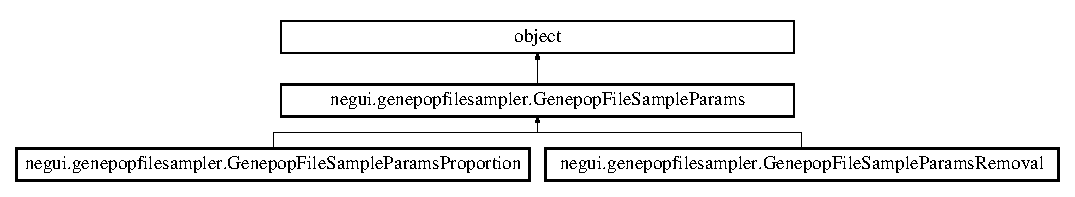
\includegraphics[height=2.193212cm]{classnegui_1_1genepopfilesampler_1_1GenepopFileSampleParams}
\end{center}
\end{figure}
\subsection*{Public Member Functions}
\begin{DoxyCompactItemize}
\item 
def \hyperlink{classnegui_1_1genepopfilesampler_1_1GenepopFileSampleParams_adb4c66f2bffa0a2eca84ed3dd3bc6385}{\+\_\+\+\_\+init\+\_\+\+\_\+} (self, li\+\_\+population\+\_\+numbers, s\+\_\+population\+\_\+subsample\+\_\+name=\char`\"{}population\+\_\+numbers\char`\"{})
\item 
def {\bfseries population\+\_\+numbers} (self)\hypertarget{classnegui_1_1genepopfilesampler_1_1GenepopFileSampleParams_a5ecc667eef35a832923e5c4ce659cfe7}{}\label{classnegui_1_1genepopfilesampler_1_1GenepopFileSampleParams_a5ecc667eef35a832923e5c4ce659cfe7}

\item 
def {\bfseries population\+\_\+subsample\+\_\+name} (self)\hypertarget{classnegui_1_1genepopfilesampler_1_1GenepopFileSampleParams_ab3ae1c545edd5230e6c37db9507d0535}{}\label{classnegui_1_1genepopfilesampler_1_1GenepopFileSampleParams_ab3ae1c545edd5230e6c37db9507d0535}

\end{DoxyCompactItemize}


\subsection{Detailed Description}
\begin{DoxyVerb}Supporting objects for GenepopFileSampler instances,
proving the sampling parameters.  For example, for 
sampling by proportions, this object would provide
a list of proportions of which each population is to 
be sampled, and a number of replicates indicating how
many samples to take at each proportion.  Further,
These objects also supply a list of population numbers,
from the range 1,2,3,...,N of the genepop files N
populations
\end{DoxyVerb}
 

Definition at line 89 of file genepopfilesampler.\+py.



\subsection{Constructor \& Destructor Documentation}
\index{negui\+::genepopfilesampler\+::\+Genepop\+File\+Sample\+Params@{negui\+::genepopfilesampler\+::\+Genepop\+File\+Sample\+Params}!\+\_\+\+\_\+init\+\_\+\+\_\+@{\+\_\+\+\_\+init\+\_\+\+\_\+}}
\index{\+\_\+\+\_\+init\+\_\+\+\_\+@{\+\_\+\+\_\+init\+\_\+\+\_\+}!negui\+::genepopfilesampler\+::\+Genepop\+File\+Sample\+Params@{negui\+::genepopfilesampler\+::\+Genepop\+File\+Sample\+Params}}
\subsubsection[{\texorpdfstring{\+\_\+\+\_\+init\+\_\+\+\_\+(self, li\+\_\+population\+\_\+numbers, s\+\_\+population\+\_\+subsample\+\_\+name=""population\+\_\+numbers"")}{__init__(self, li_population_numbers, s_population_subsample_name="population_numbers")}}]{\setlength{\rightskip}{0pt plus 5cm}def negui.\+genepopfilesampler.\+Genepop\+File\+Sample\+Params.\+\_\+\+\_\+init\+\_\+\+\_\+ (
\begin{DoxyParamCaption}
\item[{}]{self, }
\item[{}]{li\+\_\+population\+\_\+numbers, }
\item[{}]{s\+\_\+population\+\_\+subsample\+\_\+name = {\ttfamily \char`\"{}population\+\_\+numbers\char`\"{}}}
\end{DoxyParamCaption}
)}\hypertarget{classnegui_1_1genepopfilesampler_1_1GenepopFileSampleParams_adb4c66f2bffa0a2eca84ed3dd3bc6385}{}\label{classnegui_1_1genepopfilesampler_1_1GenepopFileSampleParams_adb4c66f2bffa0a2eca84ed3dd3bc6385}
\begin{DoxyVerb}Param li_populations is a list of integers,
each of i of which refers to the ith population
in the genepop file as represented by a 
genepopfilemanager object
\end{DoxyVerb}
 

Definition at line 102 of file genepopfilesampler.\+py.


\begin{DoxyCode}
102                 s\_population\_subsample\_name=\textcolor{stringliteral}{"population\_numbers"} ):
103         \textcolor{stringliteral}{'''}
104 \textcolor{stringliteral}{        Param li\_populations is a list of integers,}
105 \textcolor{stringliteral}{        each of i of which refers to the ith population}
106 \textcolor{stringliteral}{        in the genepop file as represented by a }
107 \textcolor{stringliteral}{        genepopfilemanager object}
108 \textcolor{stringliteral}{        '''}
109         self.\hyperlink{classnegui_1_1genepopfilesampler_1_1GenepopFileSampleParams_a48dfd2df4eb75dbacdc8a274cd3323ad}{\_\_populationnumbers}=li\_population\_numbers
110         self.\hyperlink{classnegui_1_1genepopfilesampler_1_1GenepopFileSampleParams_ae03531d2c9d450d7f717816a06f3a08a}{\_\_populationsubsamplename}=s\_population\_subsample\_name
111         \textcolor{keywordflow}{return}
\end{DoxyCode}


The documentation for this class was generated from the following file\+:\begin{DoxyCompactItemize}
\item 
genepopfilesampler.\+py\end{DoxyCompactItemize}

\hypertarget{classnegui_1_1genepopfilesampler_1_1GenepopFileSampleParamsAgeStructureCohorts}{}\section{negui.\+genepopfilesampler.\+Genepop\+File\+Sample\+Params\+Age\+Structure\+Cohorts Class Reference}
\label{classnegui_1_1genepopfilesampler_1_1GenepopFileSampleParamsAgeStructureCohorts}\index{negui.\+genepopfilesampler.\+Genepop\+File\+Sample\+Params\+Age\+Structure\+Cohorts@{negui.\+genepopfilesampler.\+Genepop\+File\+Sample\+Params\+Age\+Structure\+Cohorts}}
Inheritance diagram for negui.\+genepopfilesampler.\+Genepop\+File\+Sample\+Params\+Age\+Structure\+Cohorts\+:\begin{figure}[H]
\begin{center}
\leavevmode
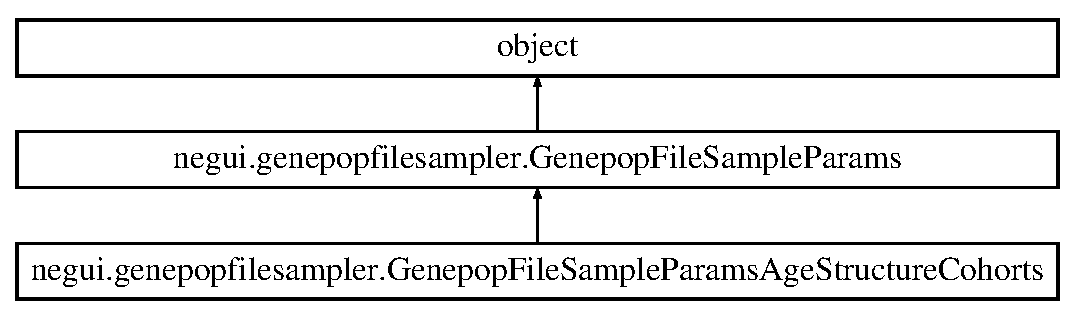
\includegraphics[height=3.000000cm]{classnegui_1_1genepopfilesampler_1_1GenepopFileSampleParamsAgeStructureCohorts}
\end{center}
\end{figure}
\subsection*{Public Member Functions}
\begin{DoxyCompactItemize}
\item 
def {\bfseries \+\_\+\+\_\+init\+\_\+\+\_\+} (self, o\+\_\+genepop\+\_\+indiv\+\_\+id\+\_\+fields, li\+\_\+population\+\_\+numbers, i\+\_\+max\+\_\+age, i\+\_\+min\+\_\+individuals\+\_\+per\+\_\+gen, i\+\_\+max\+\_\+individuals\+\_\+per\+\_\+gen, i\+\_\+ceiling\+\_\+if\+\_\+no\+\_\+total\+\_\+individuals\+\_\+per\+\_\+gen=200, lf\+\_\+proportions=None, s\+\_\+population\+\_\+subsample\+\_\+name=\char`\"{}population\+\_\+numbers\char`\"{}, i\+\_\+replicates=1, b\+\_\+lp=False, s\+\_\+sample\+\_\+param\+\_\+value=\char`\"{}c\char`\"{}, s\+\_\+sample\+\_\+tag\+\_\+base=None)\hypertarget{classnegui_1_1genepopfilesampler_1_1GenepopFileSampleParamsAgeStructureCohorts_a29b40365ec9b1944b31e86e1b770cf49}{}\label{classnegui_1_1genepopfilesampler_1_1GenepopFileSampleParamsAgeStructureCohorts_a29b40365ec9b1944b31e86e1b770cf49}

\item 
def {\bfseries fields} (self)\hypertarget{classnegui_1_1genepopfilesampler_1_1GenepopFileSampleParamsAgeStructureCohorts_a452edd8b92914959a971f988593ef260}{}\label{classnegui_1_1genepopfilesampler_1_1GenepopFileSampleParamsAgeStructureCohorts_a452edd8b92914959a971f988593ef260}

\item 
def {\bfseries max\+\_\+age} (self)\hypertarget{classnegui_1_1genepopfilesampler_1_1GenepopFileSampleParamsAgeStructureCohorts_a80713312b25a2d697db86b3324481748}{}\label{classnegui_1_1genepopfilesampler_1_1GenepopFileSampleParamsAgeStructureCohorts_a80713312b25a2d697db86b3324481748}

\item 
def {\bfseries max\+\_\+indiv\+\_\+per\+\_\+gen} (self)\hypertarget{classnegui_1_1genepopfilesampler_1_1GenepopFileSampleParamsAgeStructureCohorts_ac2f10550f834730b4b84b569008dc313}{}\label{classnegui_1_1genepopfilesampler_1_1GenepopFileSampleParamsAgeStructureCohorts_ac2f10550f834730b4b84b569008dc313}

\item 
def {\bfseries min\+\_\+indiv\+\_\+per\+\_\+gen} (self)\hypertarget{classnegui_1_1genepopfilesampler_1_1GenepopFileSampleParamsAgeStructureCohorts_a66fbdc9dab917e3ef6a42817652d0d98}{}\label{classnegui_1_1genepopfilesampler_1_1GenepopFileSampleParamsAgeStructureCohorts_a66fbdc9dab917e3ef6a42817652d0d98}

\item 
def {\bfseries proportions} (self)\hypertarget{classnegui_1_1genepopfilesampler_1_1GenepopFileSampleParamsAgeStructureCohorts_a5363ca1316f528fbd345a1697f797ed6}{}\label{classnegui_1_1genepopfilesampler_1_1GenepopFileSampleParamsAgeStructureCohorts_a5363ca1316f528fbd345a1697f797ed6}

\item 
def {\bfseries sample\+\_\+param\+\_\+value} (self)\hypertarget{classnegui_1_1genepopfilesampler_1_1GenepopFileSampleParamsAgeStructureCohorts_ad0228b1755e08ee5396a4e08eb7c4b44}{}\label{classnegui_1_1genepopfilesampler_1_1GenepopFileSampleParamsAgeStructureCohorts_ad0228b1755e08ee5396a4e08eb7c4b44}

\item 
def {\bfseries sample\+\_\+param\+\_\+value} (self, v\+\_\+value)\hypertarget{classnegui_1_1genepopfilesampler_1_1GenepopFileSampleParamsAgeStructureCohorts_a9b3e052eb9da277bb815ba963b62eac7}{}\label{classnegui_1_1genepopfilesampler_1_1GenepopFileSampleParamsAgeStructureCohorts_a9b3e052eb9da277bb815ba963b62eac7}

\end{DoxyCompactItemize}


\subsection{Detailed Description}


Definition at line 717 of file genepopfilesampler.\+py.



The documentation for this class was generated from the following file\+:\begin{DoxyCompactItemize}
\item 
genepopfilesampler.\+py\end{DoxyCompactItemize}

\hypertarget{classnegui_1_1genepopfilesampler_1_1GenepopFileSampleParamsAgeStructureRelateds}{}\section{negui.\+genepopfilesampler.\+Genepop\+File\+Sample\+Params\+Age\+Structure\+Relateds Class Reference}
\label{classnegui_1_1genepopfilesampler_1_1GenepopFileSampleParamsAgeStructureRelateds}\index{negui.\+genepopfilesampler.\+Genepop\+File\+Sample\+Params\+Age\+Structure\+Relateds@{negui.\+genepopfilesampler.\+Genepop\+File\+Sample\+Params\+Age\+Structure\+Relateds}}
Inheritance diagram for negui.\+genepopfilesampler.\+Genepop\+File\+Sample\+Params\+Age\+Structure\+Relateds\+:\begin{figure}[H]
\begin{center}
\leavevmode
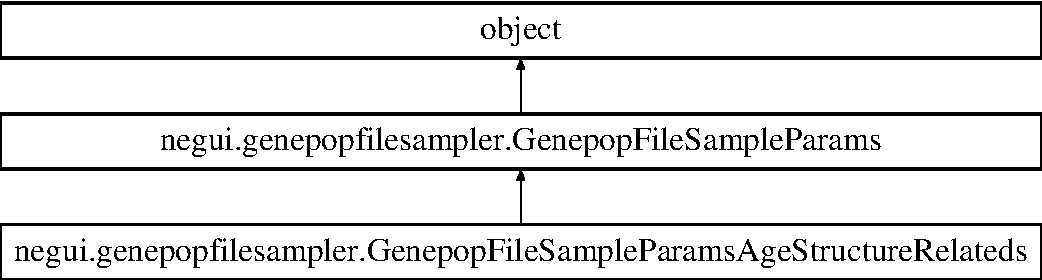
\includegraphics[height=3.000000cm]{classnegui_1_1genepopfilesampler_1_1GenepopFileSampleParamsAgeStructureRelateds}
\end{center}
\end{figure}
\subsection*{Public Member Functions}
\begin{DoxyCompactItemize}
\item 
def {\bfseries \+\_\+\+\_\+init\+\_\+\+\_\+} (self, o\+\_\+genepop\+\_\+indiv\+\_\+id\+\_\+fields, li\+\_\+population\+\_\+numbers, f\+\_\+percent\+\_\+relateds\+\_\+per\+\_\+gen, i\+\_\+min\+\_\+individuals\+\_\+per\+\_\+gen, i\+\_\+max\+\_\+individuals\+\_\+per\+\_\+gen, s\+\_\+population\+\_\+subsample\+\_\+name=\char`\"{}population\+\_\+numbers\char`\"{}, i\+\_\+replicates=1, s\+\_\+sample\+\_\+param\+\_\+value=\char`\"{}r\char`\"{}, s\+\_\+sample\+\_\+tag\+\_\+base=None)\hypertarget{classnegui_1_1genepopfilesampler_1_1GenepopFileSampleParamsAgeStructureRelateds_a251169c0b98b7430eee0fec763a94124}{}\label{classnegui_1_1genepopfilesampler_1_1GenepopFileSampleParamsAgeStructureRelateds_a251169c0b98b7430eee0fec763a94124}

\item 
def {\bfseries fields} (self)\hypertarget{classnegui_1_1genepopfilesampler_1_1GenepopFileSampleParamsAgeStructureRelateds_a863d3746d851e8b17c93a50c11ef14c4}{}\label{classnegui_1_1genepopfilesampler_1_1GenepopFileSampleParamsAgeStructureRelateds_a863d3746d851e8b17c93a50c11ef14c4}

\item 
def {\bfseries max\+\_\+indiv\+\_\+per\+\_\+gen} (self)\hypertarget{classnegui_1_1genepopfilesampler_1_1GenepopFileSampleParamsAgeStructureRelateds_ae98a0a07dffb1a63530c81f759d9f58e}{}\label{classnegui_1_1genepopfilesampler_1_1GenepopFileSampleParamsAgeStructureRelateds_ae98a0a07dffb1a63530c81f759d9f58e}

\item 
def {\bfseries min\+\_\+indiv\+\_\+per\+\_\+gen} (self)\hypertarget{classnegui_1_1genepopfilesampler_1_1GenepopFileSampleParamsAgeStructureRelateds_a6954cd905f7bb561d30215ac7e0b6954}{}\label{classnegui_1_1genepopfilesampler_1_1GenepopFileSampleParamsAgeStructureRelateds_a6954cd905f7bb561d30215ac7e0b6954}

\item 
def {\bfseries percent\+\_\+relateds} (self)\hypertarget{classnegui_1_1genepopfilesampler_1_1GenepopFileSampleParamsAgeStructureRelateds_a0112214fdc3420d19624f6de7b75ee3d}{}\label{classnegui_1_1genepopfilesampler_1_1GenepopFileSampleParamsAgeStructureRelateds_a0112214fdc3420d19624f6de7b75ee3d}

\item 
def {\bfseries sample\+\_\+param\+\_\+value} (self)\hypertarget{classnegui_1_1genepopfilesampler_1_1GenepopFileSampleParamsAgeStructureRelateds_abc3ff4bf941636c7819686bc2c06f013}{}\label{classnegui_1_1genepopfilesampler_1_1GenepopFileSampleParamsAgeStructureRelateds_abc3ff4bf941636c7819686bc2c06f013}

\end{DoxyCompactItemize}


\subsection{Detailed Description}


Definition at line 1422 of file genepopfilesampler.\+py.



The documentation for this class was generated from the following file\+:\begin{DoxyCompactItemize}
\item 
genepopfilesampler.\+py\end{DoxyCompactItemize}

\hypertarget{classnegui_1_1genepopfilesampler_1_1GenepopFileSampleParamsCohorts}{}\section{negui.\+genepopfilesampler.\+Genepop\+File\+Sample\+Params\+Cohorts Class Reference}
\label{classnegui_1_1genepopfilesampler_1_1GenepopFileSampleParamsCohorts}\index{negui.\+genepopfilesampler.\+Genepop\+File\+Sample\+Params\+Cohorts@{negui.\+genepopfilesampler.\+Genepop\+File\+Sample\+Params\+Cohorts}}
Inheritance diagram for negui.\+genepopfilesampler.\+Genepop\+File\+Sample\+Params\+Cohorts\+:\begin{figure}[H]
\begin{center}
\leavevmode
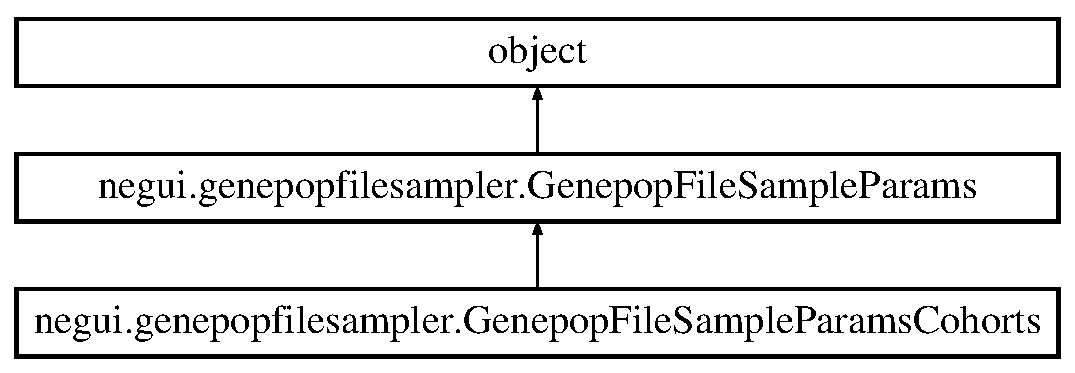
\includegraphics[height=3.000000cm]{classnegui_1_1genepopfilesampler_1_1GenepopFileSampleParamsCohorts}
\end{center}
\end{figure}
\subsection*{Public Member Functions}
\begin{DoxyCompactItemize}
\item 
def {\bfseries \+\_\+\+\_\+init\+\_\+\+\_\+} (self, o\+\_\+genepop\+\_\+indiv\+\_\+id\+\_\+fields, li\+\_\+population\+\_\+numbers, i\+\_\+max\+\_\+age, i\+\_\+min\+\_\+individuals\+\_\+per\+\_\+gen, i\+\_\+max\+\_\+individuals\+\_\+per\+\_\+gen, i\+\_\+ceiling\+\_\+if\+\_\+no\+\_\+total\+\_\+individuals\+\_\+per\+\_\+gen=200, lo\+\_\+list\+\_\+of\+\_\+value\+\_\+objects=None, s\+\_\+population\+\_\+subsample\+\_\+name=\char`\"{}population\+\_\+numbers\char`\"{}, i\+\_\+replicates=1, b\+\_\+lp=False, s\+\_\+sample\+\_\+param\+\_\+value=\char`\"{}c\char`\"{}, s\+\_\+sample\+\_\+tag\+\_\+base=None)\hypertarget{classnegui_1_1genepopfilesampler_1_1GenepopFileSampleParamsCohorts_a8c6f8f53989fc1cc18a79f89a279eb62}{}\label{classnegui_1_1genepopfilesampler_1_1GenepopFileSampleParamsCohorts_a8c6f8f53989fc1cc18a79f89a279eb62}

\item 
def {\bfseries fields} (self)\hypertarget{classnegui_1_1genepopfilesampler_1_1GenepopFileSampleParamsCohorts_abba7631b882eb94c9edc982e967e2ef2}{}\label{classnegui_1_1genepopfilesampler_1_1GenepopFileSampleParamsCohorts_abba7631b882eb94c9edc982e967e2ef2}

\item 
def {\bfseries max\+\_\+age} (self)\hypertarget{classnegui_1_1genepopfilesampler_1_1GenepopFileSampleParamsCohorts_a7c54d868b019effd0216b544888fb24d}{}\label{classnegui_1_1genepopfilesampler_1_1GenepopFileSampleParamsCohorts_a7c54d868b019effd0216b544888fb24d}

\item 
def {\bfseries max\+\_\+indiv\+\_\+per\+\_\+gen} (self)\hypertarget{classnegui_1_1genepopfilesampler_1_1GenepopFileSampleParamsCohorts_a4cbf01034bb340089a3f8608208ef201}{}\label{classnegui_1_1genepopfilesampler_1_1GenepopFileSampleParamsCohorts_a4cbf01034bb340089a3f8608208ef201}

\item 
def {\bfseries min\+\_\+indiv\+\_\+per\+\_\+gen} (self)\hypertarget{classnegui_1_1genepopfilesampler_1_1GenepopFileSampleParamsCohorts_a975ed34ec7031079d5159277e028e071}{}\label{classnegui_1_1genepopfilesampler_1_1GenepopFileSampleParamsCohorts_a975ed34ec7031079d5159277e028e071}

\item 
def {\bfseries list\+\_\+of\+\_\+sampling\+\_\+values} (self)\hypertarget{classnegui_1_1genepopfilesampler_1_1GenepopFileSampleParamsCohorts_a630cf53262bfee15371fd78a10984a5a}{}\label{classnegui_1_1genepopfilesampler_1_1GenepopFileSampleParamsCohorts_a630cf53262bfee15371fd78a10984a5a}

\item 
def {\bfseries sample\+\_\+param\+\_\+value} (self)\hypertarget{classnegui_1_1genepopfilesampler_1_1GenepopFileSampleParamsCohorts_a9e9c2215d13b79382ce6855185650097}{}\label{classnegui_1_1genepopfilesampler_1_1GenepopFileSampleParamsCohorts_a9e9c2215d13b79382ce6855185650097}

\item 
def {\bfseries sample\+\_\+param\+\_\+value} (self, v\+\_\+value)\hypertarget{classnegui_1_1genepopfilesampler_1_1GenepopFileSampleParamsCohorts_a74b4e7bc1e2bf457ce368e518f8d99d5}{}\label{classnegui_1_1genepopfilesampler_1_1GenepopFileSampleParamsCohorts_a74b4e7bc1e2bf457ce368e518f8d99d5}

\end{DoxyCompactItemize}


\subsection{Detailed Description}


Definition at line 616 of file genepopfilesampler.\+py.



The documentation for this class was generated from the following file\+:\begin{DoxyCompactItemize}
\item 
genepopfilesampler.\+py\end{DoxyCompactItemize}

\hypertarget{classnegui_1_1genepopfilesampler_1_1GenepopFileSampleParamsCriteria}{}\section{negui.\+genepopfilesampler.\+Genepop\+File\+Sample\+Params\+Criteria Class Reference}
\label{classnegui_1_1genepopfilesampler_1_1GenepopFileSampleParamsCriteria}\index{negui.\+genepopfilesampler.\+Genepop\+File\+Sample\+Params\+Criteria@{negui.\+genepopfilesampler.\+Genepop\+File\+Sample\+Params\+Criteria}}
Inheritance diagram for negui.\+genepopfilesampler.\+Genepop\+File\+Sample\+Params\+Criteria\+:\begin{figure}[H]
\begin{center}
\leavevmode
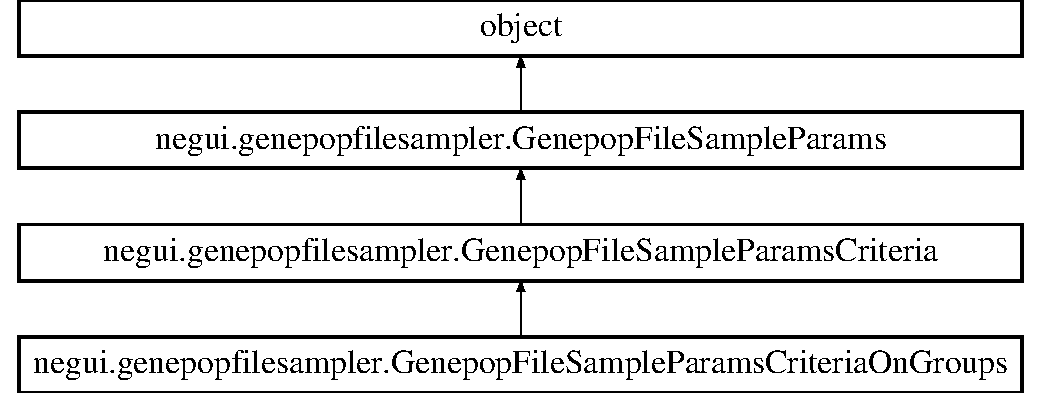
\includegraphics[height=4.000000cm]{classnegui_1_1genepopfilesampler_1_1GenepopFileSampleParamsCriteria}
\end{center}
\end{figure}
\subsection*{Public Member Functions}
\begin{DoxyCompactItemize}
\item 
def \hyperlink{classnegui_1_1genepopfilesampler_1_1GenepopFileSampleParamsCriteria_acab5979ca4ef3a3acd0843ebaf672fea}{\+\_\+\+\_\+init\+\_\+\+\_\+} (self, o\+\_\+genepop\+\_\+indiv\+\_\+id\+\_\+fields, o\+\_\+genepop\+\_\+indiv\+\_\+id\+\_\+critera, li\+\_\+population\+\_\+numbers, s\+\_\+population\+\_\+subsample\+\_\+name=\char`\"{}poplulation\+\_\+numbers\char`\"{}, i\+\_\+replicates=1, i\+\_\+min\+\_\+sampled\+\_\+pop\+\_\+size=None, i\+\_\+max\+\_\+sampled\+\_\+pop\+\_\+size=None, s\+\_\+sample\+\_\+tag\+\_\+base=None)
\item 
def {\bfseries fields} (self)\hypertarget{classnegui_1_1genepopfilesampler_1_1GenepopFileSampleParamsCriteria_a3194e915973df1a57ed9f151b5e373e3}{}\label{classnegui_1_1genepopfilesampler_1_1GenepopFileSampleParamsCriteria_a3194e915973df1a57ed9f151b5e373e3}

\item 
def {\bfseries criteria} (self)\hypertarget{classnegui_1_1genepopfilesampler_1_1GenepopFileSampleParamsCriteria_ae7e3713c18e7d30463f918dd8d90816a}{}\label{classnegui_1_1genepopfilesampler_1_1GenepopFileSampleParamsCriteria_ae7e3713c18e7d30463f918dd8d90816a}

\item 
def {\bfseries min\+\_\+sampled\+\_\+pop\+\_\+size} (self)\hypertarget{classnegui_1_1genepopfilesampler_1_1GenepopFileSampleParamsCriteria_a81389d54dc9af80c4aa90720bc9a3935}{}\label{classnegui_1_1genepopfilesampler_1_1GenepopFileSampleParamsCriteria_a81389d54dc9af80c4aa90720bc9a3935}

\item 
def {\bfseries max\+\_\+sampled\+\_\+pop\+\_\+size} (self)\hypertarget{classnegui_1_1genepopfilesampler_1_1GenepopFileSampleParamsCriteria_a8d42466bc9854e633328681f16ec0c04}{}\label{classnegui_1_1genepopfilesampler_1_1GenepopFileSampleParamsCriteria_a8d42466bc9854e633328681f16ec0c04}

\end{DoxyCompactItemize}


\subsection{Detailed Description}
\begin{DoxyVerb}Parameters for sampling scheme such that for each population
we select individuals that meet one or more criteria as 
given in the individual ID as processed by the classes in
genepopindividualid.py. 
\end{DoxyVerb}
 

Definition at line 461 of file genepopfilesampler.\+py.



\subsection{Constructor \& Destructor Documentation}
\index{negui\+::genepopfilesampler\+::\+Genepop\+File\+Sample\+Params\+Criteria@{negui\+::genepopfilesampler\+::\+Genepop\+File\+Sample\+Params\+Criteria}!\+\_\+\+\_\+init\+\_\+\+\_\+@{\+\_\+\+\_\+init\+\_\+\+\_\+}}
\index{\+\_\+\+\_\+init\+\_\+\+\_\+@{\+\_\+\+\_\+init\+\_\+\+\_\+}!negui\+::genepopfilesampler\+::\+Genepop\+File\+Sample\+Params\+Criteria@{negui\+::genepopfilesampler\+::\+Genepop\+File\+Sample\+Params\+Criteria}}
\subsubsection[{\texorpdfstring{\+\_\+\+\_\+init\+\_\+\+\_\+(self, o\+\_\+genepop\+\_\+indiv\+\_\+id\+\_\+fields, o\+\_\+genepop\+\_\+indiv\+\_\+id\+\_\+critera, li\+\_\+population\+\_\+numbers, s\+\_\+population\+\_\+subsample\+\_\+name=""poplulation\+\_\+numbers"", i\+\_\+replicates=1, i\+\_\+min\+\_\+sampled\+\_\+pop\+\_\+size=\+None, i\+\_\+max\+\_\+sampled\+\_\+pop\+\_\+size=\+None, s\+\_\+sample\+\_\+tag\+\_\+base=\+None)}{__init__(self, o_genepop_indiv_id_fields, o_genepop_indiv_id_critera, li_population_numbers, s_population_subsample_name="poplulation_numbers", i_replicates=1, i_min_sampled_pop_size=None, i_max_sampled_pop_size=None, s_sample_tag_base=None)}}]{\setlength{\rightskip}{0pt plus 5cm}def negui.\+genepopfilesampler.\+Genepop\+File\+Sample\+Params\+Criteria.\+\_\+\+\_\+init\+\_\+\+\_\+ (
\begin{DoxyParamCaption}
\item[{}]{self, }
\item[{}]{o\+\_\+genepop\+\_\+indiv\+\_\+id\+\_\+fields, }
\item[{}]{o\+\_\+genepop\+\_\+indiv\+\_\+id\+\_\+critera, }
\item[{}]{li\+\_\+population\+\_\+numbers, }
\item[{}]{s\+\_\+population\+\_\+subsample\+\_\+name = {\ttfamily \char`\"{}poplulation\+\_\+numbers\char`\"{}}, }
\item[{}]{i\+\_\+replicates = {\ttfamily 1}, }
\item[{}]{i\+\_\+min\+\_\+sampled\+\_\+pop\+\_\+size = {\ttfamily None}, }
\item[{}]{i\+\_\+max\+\_\+sampled\+\_\+pop\+\_\+size = {\ttfamily None}, }
\item[{}]{s\+\_\+sample\+\_\+tag\+\_\+base = {\ttfamily None}}
\end{DoxyParamCaption}
)}\hypertarget{classnegui_1_1genepopfilesampler_1_1GenepopFileSampleParamsCriteria_acab5979ca4ef3a3acd0843ebaf672fea}{}\label{classnegui_1_1genepopfilesampler_1_1GenepopFileSampleParamsCriteria_acab5979ca4ef3a3acd0843ebaf672fea}
\begin{DoxyVerb}param o_genepop_indiv_id_fields, instance of GenepopIndivIdFields,
param do_genepop_indiv_id_critera, dictionary of instances of 
type GenepopIndivCriterion, keyed to their member
property, "name: (__criterionname)
param li_population_numbers, list of pop numbers (in the genepop file)
to which we apply the critera
param s_population_subsample_name, see parent class
param i_replicates will usually be "1", since there should be
no variation between 2 such samplings of a genepop file.
param i_max_sampled_pop_size, if not None, is meant to be passed
    to the criteria subsampling def in a GenepopFileManager
    instance (passed by the GenepopFileSampler Instance using this
    class), so that, after all indivs have been chosen by the 
    criteria, the subsample in then reduced (if > i_max_sampled_pop_size),
    by random selection to be equal to i_max_sampled_pop_size.
    If None, then we expect the Samper instance to pass None to 
    the GenepopFileManager instance for the max, and so to ignore
    the restriction.
\end{DoxyVerb}
 

Definition at line 478 of file genepopfilesampler.\+py.


\begin{DoxyCode}
478             s\_sample\_tag\_base=\textcolor{keywordtype}{None} ):
479 
480         \textcolor{stringliteral}{'''}
481 \textcolor{stringliteral}{        param o\_genepop\_indiv\_id\_fields, instance of GenepopIndivIdFields,}
482 \textcolor{stringliteral}{        param do\_genepop\_indiv\_id\_critera, dictionary of instances of }
483 \textcolor{stringliteral}{                type GenepopIndivCriterion, keyed to their member}
484 \textcolor{stringliteral}{                property, "name: (\_\_criterionname)}
485 \textcolor{stringliteral}{        param li\_population\_numbers, list of pop numbers (in the genepop file)}
486 \textcolor{stringliteral}{                to which we apply the critera}
487 \textcolor{stringliteral}{        param s\_population\_subsample\_name, see parent class}
488 \textcolor{stringliteral}{        param i\_replicates will usually be "1", since there should be}
489 \textcolor{stringliteral}{                no variation between 2 such samplings of a genepop file.}
490 \textcolor{stringliteral}{        param i\_max\_sampled\_pop\_size, if not None, is meant to be passed}
491 \textcolor{stringliteral}{            to the criteria subsampling def in a GenepopFileManager}
492 \textcolor{stringliteral}{            instance (passed by the GenepopFileSampler Instance using this}
493 \textcolor{stringliteral}{            class), so that, after all indivs have been chosen by the }
494 \textcolor{stringliteral}{            criteria, the subsample in then reduced (if > i\_max\_sampled\_pop\_size),}
495 \textcolor{stringliteral}{            by random selection to be equal to i\_max\_sampled\_pop\_size.}
496 \textcolor{stringliteral}{            If None, then we expect the Samper instance to pass None to }
497 \textcolor{stringliteral}{            the GenepopFileManager instance for the max, and so to ignore}
498 \textcolor{stringliteral}{            the restriction.}
499 \textcolor{stringliteral}{        '''}
500 
501         GenepopFileSampleParams.\_\_init\_\_(self, 
502                     li\_population\_numbers=li\_population\_numbers, 
503                     s\_population\_subsample\_name=s\_population\_subsample\_name,
504                     s\_sample\_tag\_base=s\_sample\_tag\_base,
505                     i\_replicates=i\_replicates )
506 
507         self.\hyperlink{classnegui_1_1genepopfilesampler_1_1GenepopFileSampleParamsCriteria_ad950159801c155f299d739072af9ff4c}{\_\_fields}=o\_genepop\_indiv\_id\_fields
508         self.\hyperlink{classnegui_1_1genepopfilesampler_1_1GenepopFileSampleParamsCriteria_ac11b68eab95e37c6e6cda61a8eab8da1}{\_\_criteria}=o\_genepop\_indiv\_id\_critera
509         self.\hyperlink{classnegui_1_1genepopfilesampler_1_1GenepopFileSampleParamsCriteria_a67b43f10ef8d60f9064976531103c984}{\_\_min\_pop\_size}=i\_min\_sampled\_pop\_size
510         self.\hyperlink{classnegui_1_1genepopfilesampler_1_1GenepopFileSampleParamsCriteria_a269ebb79749ca25df7e61f84760df79c}{\_\_max\_pop\_size}=i\_max\_sampled\_pop\_size
511 
512         \textcolor{keywordflow}{return}
\end{DoxyCode}


The documentation for this class was generated from the following file\+:\begin{DoxyCompactItemize}
\item 
genepopfilesampler.\+py\end{DoxyCompactItemize}

\hypertarget{classnegui_1_1genepopfilesampler_1_1GenepopFileSampleParamsCriteriaOnGroups}{}\section{negui.\+genepopfilesampler.\+Genepop\+File\+Sample\+Params\+Criteria\+On\+Groups Class Reference}
\label{classnegui_1_1genepopfilesampler_1_1GenepopFileSampleParamsCriteriaOnGroups}\index{negui.\+genepopfilesampler.\+Genepop\+File\+Sample\+Params\+Criteria\+On\+Groups@{negui.\+genepopfilesampler.\+Genepop\+File\+Sample\+Params\+Criteria\+On\+Groups}}
Inheritance diagram for negui.\+genepopfilesampler.\+Genepop\+File\+Sample\+Params\+Criteria\+On\+Groups\+:\begin{figure}[H]
\begin{center}
\leavevmode
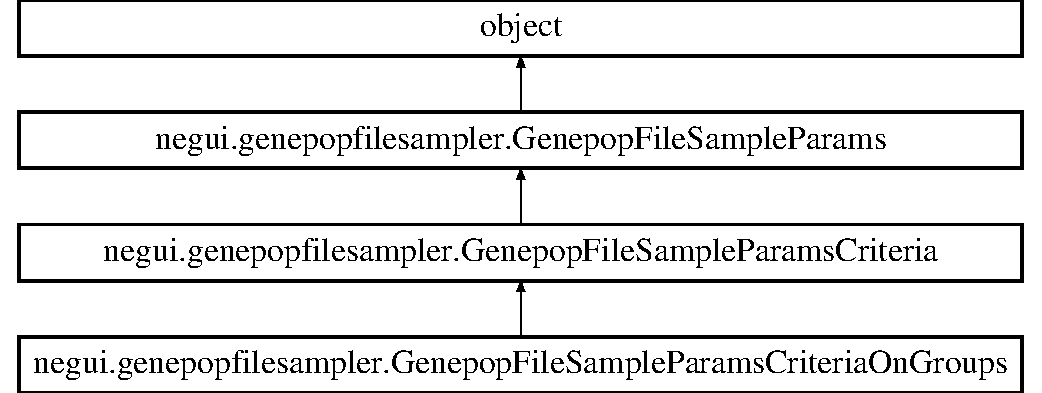
\includegraphics[height=4.000000cm]{classnegui_1_1genepopfilesampler_1_1GenepopFileSampleParamsCriteriaOnGroups}
\end{center}
\end{figure}
\subsection*{Public Member Functions}
\begin{DoxyCompactItemize}
\item 
def \hyperlink{classnegui_1_1genepopfilesampler_1_1GenepopFileSampleParamsCriteriaOnGroups_ab9e717598c2781a095bfb169b3457879}{\+\_\+\+\_\+init\+\_\+\+\_\+} (self, o\+\_\+genepop\+\_\+indiv\+\_\+id\+\_\+fields, o\+\_\+genepop\+\_\+indiv\+\_\+id\+\_\+critera, li\+\_\+population\+\_\+numbers, ls\+\_\+field\+\_\+names\+\_\+to\+\_\+group\+\_\+on, s\+\_\+population\+\_\+subsample\+\_\+name=\char`\"{}poplulation\+\_\+numbers\char`\"{}, i\+\_\+replicates=1, i\+\_\+max\+\_\+sampled\+\_\+pop\+\_\+size=None, s\+\_\+sample\+\_\+tag\+\_\+base=None)
\item 
def {\bfseries grouped\+\_\+fields} (self)\hypertarget{classnegui_1_1genepopfilesampler_1_1GenepopFileSampleParamsCriteriaOnGroups_aa7daa9e80fe3fedf4ef2303b035fead2}{}\label{classnegui_1_1genepopfilesampler_1_1GenepopFileSampleParamsCriteriaOnGroups_aa7daa9e80fe3fedf4ef2303b035fead2}

\end{DoxyCompactItemize}


\subsection{Detailed Description}
\begin{DoxyVerb}This class extends GenepopFileSampleParamsCriteria
by adding a grouping function, whereby individuals
are subsampled into groups according to whether they
match a set of one or more field values. Other criteria
can also be applied.  The member GenepopIndivCriteriaCriteria 
object can also be None, in which case subsampleing will be
Parameters for sampling scheme such that for each population
we select individuals that meet one or more criteria as 
given in the individual ID as processed by the classes in
genepopindividualid.py. 
\end{DoxyVerb}
 

Definition at line 536 of file genepopfilesampler.\+py.



\subsection{Constructor \& Destructor Documentation}
\index{negui\+::genepopfilesampler\+::\+Genepop\+File\+Sample\+Params\+Criteria\+On\+Groups@{negui\+::genepopfilesampler\+::\+Genepop\+File\+Sample\+Params\+Criteria\+On\+Groups}!\+\_\+\+\_\+init\+\_\+\+\_\+@{\+\_\+\+\_\+init\+\_\+\+\_\+}}
\index{\+\_\+\+\_\+init\+\_\+\+\_\+@{\+\_\+\+\_\+init\+\_\+\+\_\+}!negui\+::genepopfilesampler\+::\+Genepop\+File\+Sample\+Params\+Criteria\+On\+Groups@{negui\+::genepopfilesampler\+::\+Genepop\+File\+Sample\+Params\+Criteria\+On\+Groups}}
\subsubsection[{\texorpdfstring{\+\_\+\+\_\+init\+\_\+\+\_\+(self, o\+\_\+genepop\+\_\+indiv\+\_\+id\+\_\+fields, o\+\_\+genepop\+\_\+indiv\+\_\+id\+\_\+critera, li\+\_\+population\+\_\+numbers, ls\+\_\+field\+\_\+names\+\_\+to\+\_\+group\+\_\+on, s\+\_\+population\+\_\+subsample\+\_\+name=""poplulation\+\_\+numbers"", i\+\_\+replicates=1, i\+\_\+max\+\_\+sampled\+\_\+pop\+\_\+size=\+None, s\+\_\+sample\+\_\+tag\+\_\+base=\+None)}{__init__(self, o_genepop_indiv_id_fields, o_genepop_indiv_id_critera, li_population_numbers, ls_field_names_to_group_on, s_population_subsample_name="poplulation_numbers", i_replicates=1, i_max_sampled_pop_size=None, s_sample_tag_base=None)}}]{\setlength{\rightskip}{0pt plus 5cm}def negui.\+genepopfilesampler.\+Genepop\+File\+Sample\+Params\+Criteria\+On\+Groups.\+\_\+\+\_\+init\+\_\+\+\_\+ (
\begin{DoxyParamCaption}
\item[{}]{self, }
\item[{}]{o\+\_\+genepop\+\_\+indiv\+\_\+id\+\_\+fields, }
\item[{}]{o\+\_\+genepop\+\_\+indiv\+\_\+id\+\_\+critera, }
\item[{}]{li\+\_\+population\+\_\+numbers, }
\item[{}]{ls\+\_\+field\+\_\+names\+\_\+to\+\_\+group\+\_\+on, }
\item[{}]{s\+\_\+population\+\_\+subsample\+\_\+name = {\ttfamily \char`\"{}poplulation\+\_\+numbers\char`\"{}}, }
\item[{}]{i\+\_\+replicates = {\ttfamily 1}, }
\item[{}]{i\+\_\+max\+\_\+sampled\+\_\+pop\+\_\+size = {\ttfamily None}, }
\item[{}]{s\+\_\+sample\+\_\+tag\+\_\+base = {\ttfamily None}}
\end{DoxyParamCaption}
)}\hypertarget{classnegui_1_1genepopfilesampler_1_1GenepopFileSampleParamsCriteriaOnGroups_ab9e717598c2781a095bfb169b3457879}{}\label{classnegui_1_1genepopfilesampler_1_1GenepopFileSampleParamsCriteriaOnGroups_ab9e717598c2781a095bfb169b3457879}
\begin{DoxyVerb}param o_genepop_indiv_id_fields, instance of GenepopIndivIdFields,
param do_genepop_indiv_id_critera, dictionary of instances of 
type GenepopIndivCriterion, keyed to their member
property, "name: (__criterionname)
param li_population_numbers, list of pop numbers (in the genepop file)
to which we apply the critera.
param ls_field_names_to_group_on, list of strings, field names, 
on which to group individuals.  These unique sets of
field values will then be used as criteria in subsampling.
param s_population_subsample_name, see parent class
param i_replicates will usually be "1", since there should be
no variation between 2 such samplings of a genepop file.
param i_max_sampled_pop_size, if not None, is meant to be passed
    to the criteria subsampling def in a GenepopFileManager
    instance (passed by the GenepopFileSampler Instance using this
    class), so that, after all indivs have been chosen by the 
    criteria, the subsample in then reduced (if > i_max_sampled_pop_size),
    by random selection to be equal to i_max_sampled_pop_size.
    If None, then we expect the Samper instance to pass None to 
    the GenepopFileManager instance for the max, and so to ignore
    the restriction.
\end{DoxyVerb}
 

Definition at line 560 of file genepopfilesampler.\+py.


\begin{DoxyCode}
560                 s\_sample\_tag\_base=\textcolor{keywordtype}{None} ):
561 
562         \textcolor{stringliteral}{'''}
563 \textcolor{stringliteral}{        param o\_genepop\_indiv\_id\_fields, instance of GenepopIndivIdFields,}
564 \textcolor{stringliteral}{        param do\_genepop\_indiv\_id\_critera, dictionary of instances of }
565 \textcolor{stringliteral}{                type GenepopIndivCriterion, keyed to their member}
566 \textcolor{stringliteral}{                property, "name: (\_\_criterionname)}
567 \textcolor{stringliteral}{        param li\_population\_numbers, list of pop numbers (in the genepop file)}
568 \textcolor{stringliteral}{                to which we apply the critera.}
569 \textcolor{stringliteral}{        param ls\_field\_names\_to\_group\_on, list of strings, field names, }
570 \textcolor{stringliteral}{                on which to group individuals.  These unique sets of}
571 \textcolor{stringliteral}{                field values will then be used as criteria in subsampling.}
572 \textcolor{stringliteral}{        param s\_population\_subsample\_name, see parent class}
573 \textcolor{stringliteral}{        param i\_replicates will usually be "1", since there should be}
574 \textcolor{stringliteral}{                no variation between 2 such samplings of a genepop file.}
575 \textcolor{stringliteral}{        param i\_max\_sampled\_pop\_size, if not None, is meant to be passed}
576 \textcolor{stringliteral}{            to the criteria subsampling def in a GenepopFileManager}
577 \textcolor{stringliteral}{            instance (passed by the GenepopFileSampler Instance using this}
578 \textcolor{stringliteral}{            class), so that, after all indivs have been chosen by the }
579 \textcolor{stringliteral}{            criteria, the subsample in then reduced (if > i\_max\_sampled\_pop\_size),}
580 \textcolor{stringliteral}{            by random selection to be equal to i\_max\_sampled\_pop\_size.}
581 \textcolor{stringliteral}{            If None, then we expect the Samper instance to pass None to }
582 \textcolor{stringliteral}{            the GenepopFileManager instance for the max, and so to ignore}
583 \textcolor{stringliteral}{            the restriction.}
584 \textcolor{stringliteral}{        '''}
585 
586         GenepopFileSampleParamsCriteria.\_\_init\_\_( \(\backslash\)
587                     self, 
588                     o\_genepop\_indiv\_id\_fields,
589                     o\_genepop\_indiv\_id\_critera,
590                     li\_population\_numbers=li\_population\_numbers, 
591                     s\_population\_subsample\_name=s\_population\_subsample\_name,
592                     i\_replicates=i\_replicates, 
593                     i\_max\_sampled\_pop\_size=\textcolor{keywordtype}{None},
594                     s\_sample\_tag\_base=s\_sample\_tag\_base )
595 
596         
597         self.\_\_grouped\_fields
598         \textcolor{keywordflow}{return}
\end{DoxyCode}


The documentation for this class was generated from the following file\+:\begin{DoxyCompactItemize}
\item 
genepopfilesampler.\+py\end{DoxyCompactItemize}

\hypertarget{classnegui_1_1genepopfilesampler_1_1GenepopFileSampleParamsLoci}{}\section{negui.\+genepopfilesampler.\+Genepop\+File\+Sample\+Params\+Loci Class Reference}
\label{classnegui_1_1genepopfilesampler_1_1GenepopFileSampleParamsLoci}\index{negui.\+genepopfilesampler.\+Genepop\+File\+Sample\+Params\+Loci@{negui.\+genepopfilesampler.\+Genepop\+File\+Sample\+Params\+Loci}}
Inheritance diagram for negui.\+genepopfilesampler.\+Genepop\+File\+Sample\+Params\+Loci\+:\begin{figure}[H]
\begin{center}
\leavevmode
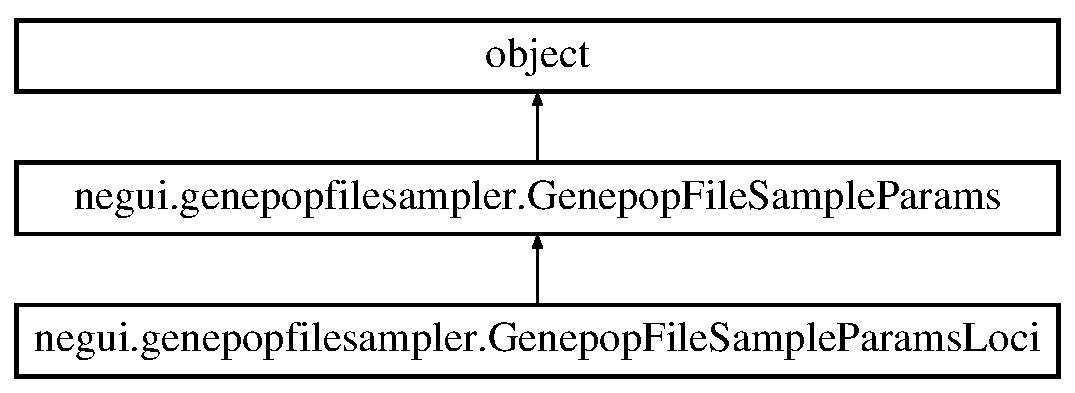
\includegraphics[height=3.000000cm]{classnegui_1_1genepopfilesampler_1_1GenepopFileSampleParamsLoci}
\end{center}
\end{figure}
\subsection*{Public Member Functions}
\begin{DoxyCompactItemize}
\item 
def {\bfseries \+\_\+\+\_\+init\+\_\+\+\_\+} (self, li\+\_\+population\+\_\+numbers, i\+\_\+min\+\_\+loci\+\_\+position, i\+\_\+max\+\_\+loci\+\_\+position, i\+\_\+max\+\_\+total\+\_\+loci=None, i\+\_\+min\+\_\+total\+\_\+loci=None, lf\+\_\+proportions=None, li\+\_\+sample\+\_\+totals=None, i\+\_\+replicates=1, s\+\_\+population\+\_\+subsample\+\_\+name=\char`\"{}population\+\_\+numbers\char`\"{}, v\+\_\+sample\+\_\+value=\char`\"{}rt\char`\"{}, s\+\_\+sample\+\_\+tag\+\_\+base=None)\hypertarget{classnegui_1_1genepopfilesampler_1_1GenepopFileSampleParamsLoci_abae84ffce06e7bfe793e4eab12176e9d}{}\label{classnegui_1_1genepopfilesampler_1_1GenepopFileSampleParamsLoci_abae84ffce06e7bfe793e4eab12176e9d}

\item 
def {\bfseries min\+\_\+loci\+\_\+position} (self)\hypertarget{classnegui_1_1genepopfilesampler_1_1GenepopFileSampleParamsLoci_a538126db0b2cbb0070d90fd82e846e95}{}\label{classnegui_1_1genepopfilesampler_1_1GenepopFileSampleParamsLoci_a538126db0b2cbb0070d90fd82e846e95}

\item 
def {\bfseries max\+\_\+loci\+\_\+position} (self)\hypertarget{classnegui_1_1genepopfilesampler_1_1GenepopFileSampleParamsLoci_a35010147e4f3dc839fcc7bc3d6f31e3b}{}\label{classnegui_1_1genepopfilesampler_1_1GenepopFileSampleParamsLoci_a35010147e4f3dc839fcc7bc3d6f31e3b}

\item 
def {\bfseries min\+\_\+total\+\_\+loci} (self)\hypertarget{classnegui_1_1genepopfilesampler_1_1GenepopFileSampleParamsLoci_ad3b3944904c30ac3b4b5760f48b223b4}{}\label{classnegui_1_1genepopfilesampler_1_1GenepopFileSampleParamsLoci_ad3b3944904c30ac3b4b5760f48b223b4}

\item 
def {\bfseries max\+\_\+total\+\_\+loci} (self)\hypertarget{classnegui_1_1genepopfilesampler_1_1GenepopFileSampleParamsLoci_afd60b83e499e8fe3ab17d1248f970490}{}\label{classnegui_1_1genepopfilesampler_1_1GenepopFileSampleParamsLoci_afd60b83e499e8fe3ab17d1248f970490}

\item 
def {\bfseries sample\+\_\+param\+\_\+value} (self)\hypertarget{classnegui_1_1genepopfilesampler_1_1GenepopFileSampleParamsLoci_a19285822eed17d73e84c74b82179de3c}{}\label{classnegui_1_1genepopfilesampler_1_1GenepopFileSampleParamsLoci_a19285822eed17d73e84c74b82179de3c}

\item 
def {\bfseries proportions} (self)\hypertarget{classnegui_1_1genepopfilesampler_1_1GenepopFileSampleParamsLoci_ab34f0100656df6bb9e6c7c02d72b9a71}{}\label{classnegui_1_1genepopfilesampler_1_1GenepopFileSampleParamsLoci_ab34f0100656df6bb9e6c7c02d72b9a71}

\item 
def {\bfseries sample\+\_\+totals} (self)\hypertarget{classnegui_1_1genepopfilesampler_1_1GenepopFileSampleParamsLoci_a28de868054462f16d6ed84944ce248b1}{}\label{classnegui_1_1genepopfilesampler_1_1GenepopFileSampleParamsLoci_a28de868054462f16d6ed84944ce248b1}

\end{DoxyCompactItemize}


\subsection{Detailed Description}
\begin{DoxyVerb}Parameter set for sampling loci from the ith to the jth, 
as listed in the genepop file individual entries. 
Also provides for a max_total_loci, to trunctate the total loci 
to this number by random sampling. Also provides a propotioin value,
if needed, for randomly sampling a proportion of the loci within
the given range.  See classs below, GenepopFileSamplerLociByRangeAndTotal and
GenepopFileSampleParamsLociByRangeAndPercentage
\end{DoxyVerb}
 

Definition at line 257 of file genepopfilesampler.\+py.



The documentation for this class was generated from the following file\+:\begin{DoxyCompactItemize}
\item 
genepopfilesampler.\+py\end{DoxyCompactItemize}

\hypertarget{classnegui_1_1genepopfilesampler_1_1GenepopFileSampleParamsNone}{}\section{negui.\+genepopfilesampler.\+Genepop\+File\+Sample\+Params\+None Class Reference}
\label{classnegui_1_1genepopfilesampler_1_1GenepopFileSampleParamsNone}\index{negui.\+genepopfilesampler.\+Genepop\+File\+Sample\+Params\+None@{negui.\+genepopfilesampler.\+Genepop\+File\+Sample\+Params\+None}}
Inheritance diagram for negui.\+genepopfilesampler.\+Genepop\+File\+Sample\+Params\+None\+:\begin{figure}[H]
\begin{center}
\leavevmode
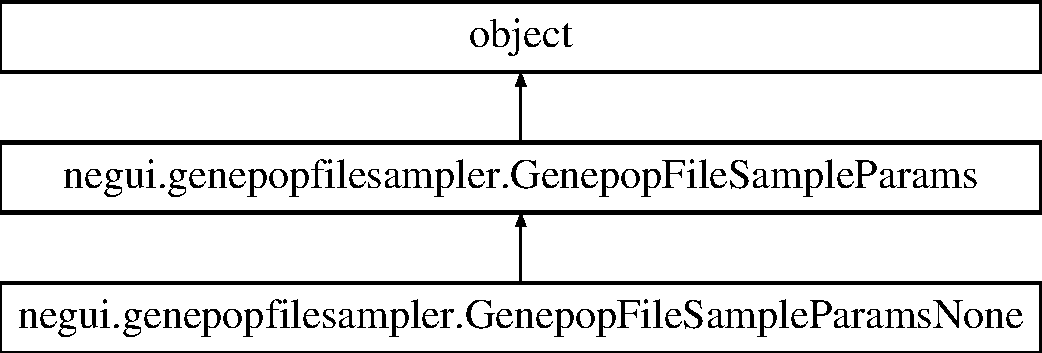
\includegraphics[height=3.000000cm]{classnegui_1_1genepopfilesampler_1_1GenepopFileSampleParamsNone}
\end{center}
\end{figure}
\subsection*{Public Member Functions}
\begin{DoxyCompactItemize}
\item 
def {\bfseries \+\_\+\+\_\+init\+\_\+\+\_\+} (self, li\+\_\+population\+\_\+numbers, i\+\_\+min\+\_\+pop\+\_\+size, i\+\_\+max\+\_\+pop\+\_\+size, i\+\_\+replicates=1, s\+\_\+population\+\_\+subsample\+\_\+name=\char`\"{}population\+\_\+numbers\char`\"{}, v\+\_\+sample\+\_\+value=\char`\"{}n\char`\"{}, s\+\_\+sample\+\_\+tag\+\_\+base=None)\hypertarget{classnegui_1_1genepopfilesampler_1_1GenepopFileSampleParamsNone_a9c15bff6784a5e932e4596b7496f2ee3}{}\label{classnegui_1_1genepopfilesampler_1_1GenepopFileSampleParamsNone_a9c15bff6784a5e932e4596b7496f2ee3}

\item 
def {\bfseries min\+\_\+pop\+\_\+size} (self)\hypertarget{classnegui_1_1genepopfilesampler_1_1GenepopFileSampleParamsNone_a8410a7aa885f2155947076d344433a04}{}\label{classnegui_1_1genepopfilesampler_1_1GenepopFileSampleParamsNone_a8410a7aa885f2155947076d344433a04}

\item 
def {\bfseries max\+\_\+pop\+\_\+size} (self)\hypertarget{classnegui_1_1genepopfilesampler_1_1GenepopFileSampleParamsNone_a4c67d4b3d1124570c54b09cbe54b674a}{}\label{classnegui_1_1genepopfilesampler_1_1GenepopFileSampleParamsNone_a4c67d4b3d1124570c54b09cbe54b674a}

\item 
def {\bfseries sample\+\_\+param\+\_\+value} (self)\hypertarget{classnegui_1_1genepopfilesampler_1_1GenepopFileSampleParamsNone_add5270b7e6e3e36502cf48fe6bd3e5d0}{}\label{classnegui_1_1genepopfilesampler_1_1GenepopFileSampleParamsNone_add5270b7e6e3e36502cf48fe6bd3e5d0}

\end{DoxyCompactItemize}


\subsection{Detailed Description}
\begin{DoxyVerb}No selection of individuals, only a min/max for indiv count
per population.  If max exceeded, then sampler randomly 
selectes individuals.
\end{DoxyVerb}
 

Definition at line 333 of file genepopfilesampler.\+py.



The documentation for this class was generated from the following file\+:\begin{DoxyCompactItemize}
\item 
genepopfilesampler.\+py\end{DoxyCompactItemize}

\hypertarget{classnegui_1_1genepopfilesampler_1_1GenepopFileSampleParamsProportion}{}\section{negui.\+genepopfilesampler.\+Genepop\+File\+Sample\+Params\+Proportion Class Reference}
\label{classnegui_1_1genepopfilesampler_1_1GenepopFileSampleParamsProportion}\index{negui.\+genepopfilesampler.\+Genepop\+File\+Sample\+Params\+Proportion@{negui.\+genepopfilesampler.\+Genepop\+File\+Sample\+Params\+Proportion}}
Inheritance diagram for negui.\+genepopfilesampler.\+Genepop\+File\+Sample\+Params\+Proportion\+:\begin{figure}[H]
\begin{center}
\leavevmode
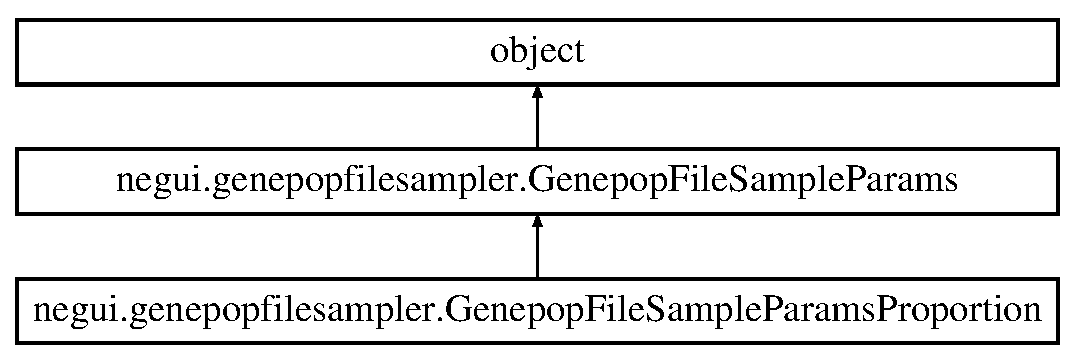
\includegraphics[height=3.000000cm]{classnegui_1_1genepopfilesampler_1_1GenepopFileSampleParamsProportion}
\end{center}
\end{figure}
\subsection*{Public Member Functions}
\begin{DoxyCompactItemize}
\item 
def \hyperlink{classnegui_1_1genepopfilesampler_1_1GenepopFileSampleParamsProportion_ab75eceef987c513501a5d55fb7ef3f7b}{\+\_\+\+\_\+init\+\_\+\+\_\+} (self, li\+\_\+population\+\_\+numbers, lf\+\_\+proportions, i\+\_\+replicates, s\+\_\+population\+\_\+subsample\+\_\+name=\char`\"{}population\+\_\+numbers\char`\"{}, s\+\_\+sample\+\_\+tag\+\_\+base=None)
\item 
def {\bfseries proportions} (self)\hypertarget{classnegui_1_1genepopfilesampler_1_1GenepopFileSampleParamsProportion_a0b564f11df13b230af1cb7a86e1376e1}{}\label{classnegui_1_1genepopfilesampler_1_1GenepopFileSampleParamsProportion_a0b564f11df13b230af1cb7a86e1376e1}

\end{DoxyCompactItemize}


\subsection{Detailed Description}


Definition at line 377 of file genepopfilesampler.\+py.



\subsection{Constructor \& Destructor Documentation}
\index{negui\+::genepopfilesampler\+::\+Genepop\+File\+Sample\+Params\+Proportion@{negui\+::genepopfilesampler\+::\+Genepop\+File\+Sample\+Params\+Proportion}!\+\_\+\+\_\+init\+\_\+\+\_\+@{\+\_\+\+\_\+init\+\_\+\+\_\+}}
\index{\+\_\+\+\_\+init\+\_\+\+\_\+@{\+\_\+\+\_\+init\+\_\+\+\_\+}!negui\+::genepopfilesampler\+::\+Genepop\+File\+Sample\+Params\+Proportion@{negui\+::genepopfilesampler\+::\+Genepop\+File\+Sample\+Params\+Proportion}}
\subsubsection[{\texorpdfstring{\+\_\+\+\_\+init\+\_\+\+\_\+(self, li\+\_\+population\+\_\+numbers, lf\+\_\+proportions, i\+\_\+replicates, s\+\_\+population\+\_\+subsample\+\_\+name=""population\+\_\+numbers"", s\+\_\+sample\+\_\+tag\+\_\+base=\+None)}{__init__(self, li_population_numbers, lf_proportions, i_replicates, s_population_subsample_name="population_numbers", s_sample_tag_base=None)}}]{\setlength{\rightskip}{0pt plus 5cm}def negui.\+genepopfilesampler.\+Genepop\+File\+Sample\+Params\+Proportion.\+\_\+\+\_\+init\+\_\+\+\_\+ (
\begin{DoxyParamCaption}
\item[{}]{self, }
\item[{}]{li\+\_\+population\+\_\+numbers, }
\item[{}]{lf\+\_\+proportions, }
\item[{}]{i\+\_\+replicates, }
\item[{}]{s\+\_\+population\+\_\+subsample\+\_\+name = {\ttfamily \char`\"{}population\+\_\+numbers\char`\"{}}, }
\item[{}]{s\+\_\+sample\+\_\+tag\+\_\+base = {\ttfamily None}}
\end{DoxyParamCaption}
)}\hypertarget{classnegui_1_1genepopfilesampler_1_1GenepopFileSampleParamsProportion_ab75eceef987c513501a5d55fb7ef3f7b}{}\label{classnegui_1_1genepopfilesampler_1_1GenepopFileSampleParamsProportion_ab75eceef987c513501a5d55fb7ef3f7b}
\begin{DoxyVerb}param li_populations, list of ints, which pops to sample (see remarks, parant class )
param lf_proportions, list of floats, each pop sampled at each of these proportions
param i_replicates, one integer, each pop sampled at each proportion this many times
GenepopFileSampleParams.__init__( self, li_populations )
\end{DoxyVerb}
 

Definition at line 382 of file genepopfilesampler.\+py.


\begin{DoxyCode}
382             s\_sample\_tag\_base=\textcolor{keywordtype}{None} ):
383 
384         \textcolor{stringliteral}{'''}
385 \textcolor{stringliteral}{        param li\_populations, list of ints, which pops to sample (see remarks, parant class )}
386 \textcolor{stringliteral}{        param lf\_proportions, list of floats, each pop sampled at each of these proportions}
387 \textcolor{stringliteral}{        param i\_replicates, one integer, each pop sampled at each proportion this many times}
388 \textcolor{stringliteral}{        GenepopFileSampleParams.\_\_init\_\_( self, li\_populations )}
389 \textcolor{stringliteral}{        '''}
390 
391         GenepopFileSampleParams.\_\_init\_\_(self, li\_population\_numbers=li\_population\_numbers, 
392                                             s\_population\_subsample\_name=s\_population\_subsample\_name,
393                                             s\_sample\_tag\_base=s\_sample\_tag\_base,
394                                             i\_replicates=i\_replicates )
395         self.\hyperlink{classnegui_1_1genepopfilesampler_1_1GenepopFileSampleParamsProportion_aa8dd8cef783da4e9bdb7c550e56382fd}{\_\_proportions}=lf\_proportions
396         \textcolor{keywordflow}{return}
\end{DoxyCode}


The documentation for this class was generated from the following file\+:\begin{DoxyCompactItemize}
\item 
genepopfilesampler.\+py\end{DoxyCompactItemize}

\hypertarget{classnegui_1_1genepopfilesampler_1_1GenepopFileSampleParamsRemoval}{}\section{negui.\+genepopfilesampler.\+Genepop\+File\+Sample\+Params\+Removal Class Reference}
\label{classnegui_1_1genepopfilesampler_1_1GenepopFileSampleParamsRemoval}\index{negui.\+genepopfilesampler.\+Genepop\+File\+Sample\+Params\+Removal@{negui.\+genepopfilesampler.\+Genepop\+File\+Sample\+Params\+Removal}}
Inheritance diagram for negui.\+genepopfilesampler.\+Genepop\+File\+Sample\+Params\+Removal\+:\begin{figure}[H]
\begin{center}
\leavevmode
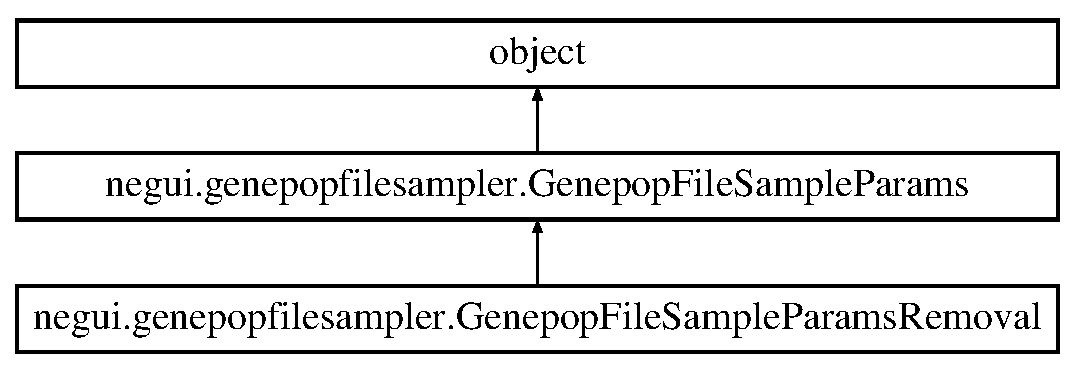
\includegraphics[height=3.000000cm]{classnegui_1_1genepopfilesampler_1_1GenepopFileSampleParamsRemoval}
\end{center}
\end{figure}
\subsection*{Public Member Functions}
\begin{DoxyCompactItemize}
\item 
def \hyperlink{classnegui_1_1genepopfilesampler_1_1GenepopFileSampleParamsRemoval_a4eb7dd24a224c024d50c3bc7f99fe283}{\+\_\+\+\_\+init\+\_\+\+\_\+} (self, li\+\_\+population\+\_\+numbers, li\+\_\+n\+\_\+to\+\_\+remove, i\+\_\+replicates, s\+\_\+population\+\_\+subsample\+\_\+name=\char`\"{}poplulation\+\_\+numbers\char`\"{}, b\+\_\+do\+\_\+all\+\_\+combos\+\_\+when\+\_\+n\+\_\+equals\+\_\+one=True)
\item 
def {\bfseries n\+\_\+to\+\_\+remove} (self)\hypertarget{classnegui_1_1genepopfilesampler_1_1GenepopFileSampleParamsRemoval_a7621d89a31284b0d6d8b49598eb1860d}{}\label{classnegui_1_1genepopfilesampler_1_1GenepopFileSampleParamsRemoval_a7621d89a31284b0d6d8b49598eb1860d}

\item 
def {\bfseries replicates} (self)\hypertarget{classnegui_1_1genepopfilesampler_1_1GenepopFileSampleParamsRemoval_a78561df77c45519715a9dd14bdfd23a0}{}\label{classnegui_1_1genepopfilesampler_1_1GenepopFileSampleParamsRemoval_a78561df77c45519715a9dd14bdfd23a0}

\item 
def {\bfseries do\+\_\+all\+\_\+combos\+\_\+when\+\_\+n\+\_\+equals\+\_\+one} (self)\hypertarget{classnegui_1_1genepopfilesampler_1_1GenepopFileSampleParamsRemoval_a6999b2175c9660123c62495ff155ad08}{}\label{classnegui_1_1genepopfilesampler_1_1GenepopFileSampleParamsRemoval_a6999b2175c9660123c62495ff155ad08}

\end{DoxyCompactItemize}


\subsection{Detailed Description}
\begin{DoxyVerb}Parameters for sampling scheme such that for each population
we randomly remove N of the M individuals, removing all M where
N>=M, repeating i_replicate times. 

When the b_do_all_combos_when_n_equals_one flag in __init__ is
set to True (the default), we treat N=1 differently, and 
exhaust all possible removals -- i.e, in each pop_i 
of size M_i, removing each N where N=1,2,3...M_i.
\end{DoxyVerb}
 

Definition at line 158 of file genepopfilesampler.\+py.



\subsection{Constructor \& Destructor Documentation}
\index{negui\+::genepopfilesampler\+::\+Genepop\+File\+Sample\+Params\+Removal@{negui\+::genepopfilesampler\+::\+Genepop\+File\+Sample\+Params\+Removal}!\+\_\+\+\_\+init\+\_\+\+\_\+@{\+\_\+\+\_\+init\+\_\+\+\_\+}}
\index{\+\_\+\+\_\+init\+\_\+\+\_\+@{\+\_\+\+\_\+init\+\_\+\+\_\+}!negui\+::genepopfilesampler\+::\+Genepop\+File\+Sample\+Params\+Removal@{negui\+::genepopfilesampler\+::\+Genepop\+File\+Sample\+Params\+Removal}}
\subsubsection[{\texorpdfstring{\+\_\+\+\_\+init\+\_\+\+\_\+(self, li\+\_\+population\+\_\+numbers, li\+\_\+n\+\_\+to\+\_\+remove, i\+\_\+replicates, s\+\_\+population\+\_\+subsample\+\_\+name=""poplulation\+\_\+numbers"", b\+\_\+do\+\_\+all\+\_\+combos\+\_\+when\+\_\+n\+\_\+equals\+\_\+one=\+True)}{__init__(self, li_population_numbers, li_n_to_remove, i_replicates, s_population_subsample_name="poplulation_numbers", b_do_all_combos_when_n_equals_one=True)}}]{\setlength{\rightskip}{0pt plus 5cm}def negui.\+genepopfilesampler.\+Genepop\+File\+Sample\+Params\+Removal.\+\_\+\+\_\+init\+\_\+\+\_\+ (
\begin{DoxyParamCaption}
\item[{}]{self, }
\item[{}]{li\+\_\+population\+\_\+numbers, }
\item[{}]{li\+\_\+n\+\_\+to\+\_\+remove, }
\item[{}]{i\+\_\+replicates, }
\item[{}]{s\+\_\+population\+\_\+subsample\+\_\+name = {\ttfamily \char`\"{}poplulation\+\_\+numbers\char`\"{}}, }
\item[{}]{b\+\_\+do\+\_\+all\+\_\+combos\+\_\+when\+\_\+n\+\_\+equals\+\_\+one = {\ttfamily True}}
\end{DoxyParamCaption}
)}\hypertarget{classnegui_1_1genepopfilesampler_1_1GenepopFileSampleParamsRemoval_a4eb7dd24a224c024d50c3bc7f99fe283}{}\label{classnegui_1_1genepopfilesampler_1_1GenepopFileSampleParamsRemoval_a4eb7dd24a224c024d50c3bc7f99fe283}
\begin{DoxyVerb}param li_population_numbers, list of ints, see parent class
param li_n_to_remove, list of ints, indicating, for each pop, randomly 
      remove n individuals
param i_replicates, for each i_n, repeat i_replicates times
param s_population_subsample_name, see parent class
param b_do_all_combos_when_n_equals_one -- if true treat n=1 differently,
      by repeating a remove-one-indiv for each indiv in each pop.
\end{DoxyVerb}
 

Definition at line 176 of file genepopfilesampler.\+py.


\begin{DoxyCode}
176             b\_do\_all\_combos\_when\_n\_equals\_one=\textcolor{keyword}{True} ):
177         \textcolor{stringliteral}{'''}
178 \textcolor{stringliteral}{        param li\_population\_numbers, list of ints, see parent class}
179 \textcolor{stringliteral}{        param li\_n\_to\_remove, list of ints, indicating, for each pop, randomly }
180 \textcolor{stringliteral}{              remove n individuals}
181 \textcolor{stringliteral}{        param i\_replicates, for each i\_n, repeat i\_replicates times}
182 \textcolor{stringliteral}{        param s\_population\_subsample\_name, see parent class}
183 \textcolor{stringliteral}{        param b\_do\_all\_combos\_when\_n\_equals\_one -- if true treat n=1 differently,}
184 \textcolor{stringliteral}{              by repeating a remove-one-indiv for each indiv in each pop.}
185 \textcolor{stringliteral}{        '''}
186 
187         GenepopFileSampleParams.\_\_init\_\_(self, 
188                     li\_population\_numbers=li\_population\_numbers, 
189                     s\_population\_subsample\_name=s\_population\_subsample\_name )
190 
191         self.\hyperlink{classnegui_1_1genepopfilesampler_1_1GenepopFileSampleParamsRemoval_a23d601163d8118b7af9acf6acf78eecf}{\_\_n\_to\_remove}=li\_n\_to\_remove
192         self.\hyperlink{classnegui_1_1genepopfilesampler_1_1GenepopFileSampleParamsRemoval_ae2a4f45ac6b5377f749dc84a560dbf01}{\_\_replicates}=i\_replicates
193         self.\hyperlink{classnegui_1_1genepopfilesampler_1_1GenepopFileSampleParamsRemoval_a24a47d9cdac499238a1368dcc626e8a3}{\_\_do\_all\_combos\_when\_n\_equals\_one}=
      b\_do\_all\_combos\_when\_n\_equals\_one
194         \textcolor{keywordflow}{return}
\end{DoxyCode}


The documentation for this class was generated from the following file\+:\begin{DoxyCompactItemize}
\item 
genepopfilesampler.\+py\end{DoxyCompactItemize}

\hypertarget{classnegui_1_1genepopfilesampler_1_1GenepopFileSampler}{}\section{negui.\+genepopfilesampler.\+Genepop\+File\+Sampler Class Reference}
\label{classnegui_1_1genepopfilesampler_1_1GenepopFileSampler}\index{negui.\+genepopfilesampler.\+Genepop\+File\+Sampler@{negui.\+genepopfilesampler.\+Genepop\+File\+Sampler}}
Inheritance diagram for negui.\+genepopfilesampler.\+Genepop\+File\+Sampler\+:\begin{figure}[H]
\begin{center}
\leavevmode
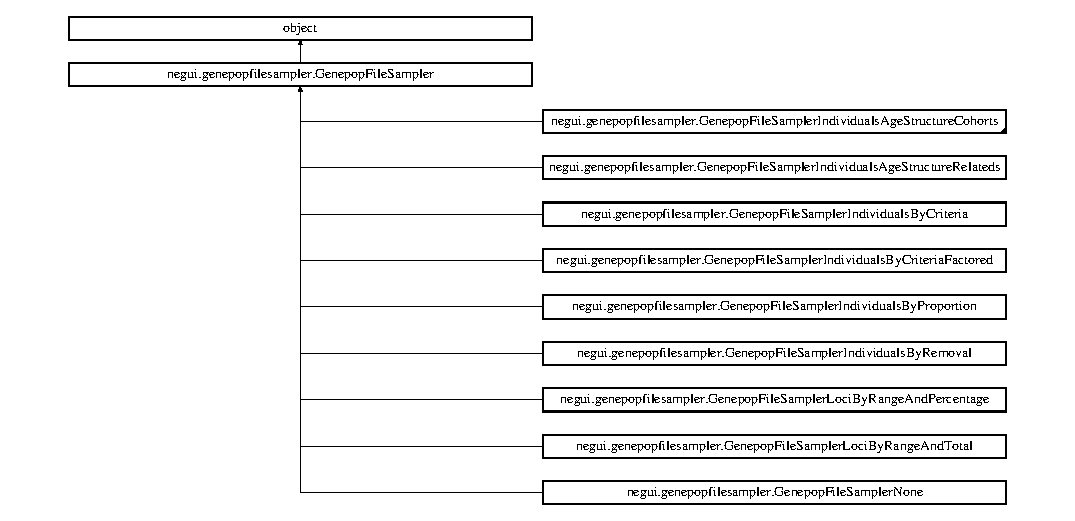
\includegraphics[height=5.957447cm]{classnegui_1_1genepopfilesampler_1_1GenepopFileSampler}
\end{center}
\end{figure}
\subsection*{Public Member Functions}
\begin{DoxyCompactItemize}
\item 
def {\bfseries \+\_\+\+\_\+init\+\_\+\+\_\+} (self, o\+\_\+genepopfilemanager, o\+\_\+genepopfilesampleparams)\hypertarget{classnegui_1_1genepopfilesampler_1_1GenepopFileSampler_abcaee019cd11b009568dde7fa2e94341}{}\label{classnegui_1_1genepopfilesampler_1_1GenepopFileSampler_abcaee019cd11b009568dde7fa2e94341}

\item 
def {\bfseries filemanager} (self)\hypertarget{classnegui_1_1genepopfilesampler_1_1GenepopFileSampler_a58431ed64951ef4a3cf813c9ee2624b3}{}\label{classnegui_1_1genepopfilesampler_1_1GenepopFileSampler_a58431ed64951ef4a3cf813c9ee2624b3}

\item 
def {\bfseries sampleparams} (self)\hypertarget{classnegui_1_1genepopfilesampler_1_1GenepopFileSampler_ad48f60ff378a777538a886b058eb0e00}{}\label{classnegui_1_1genepopfilesampler_1_1GenepopFileSampler_ad48f60ff378a777538a886b058eb0e00}

\end{DoxyCompactItemize}


\subsection{Detailed Description}
\begin{DoxyVerb}Class GenepopFileSampler instances operate on GenepopFileManager objects,
adding subsamples to the GenepopFileManager's subsample according to one of
mulitple sampling schemes.  It's chief motivation is a need to enccapsulate 
a session in which a large number of samples need to be taken from a single
genepop file, according to one of various possible sampling schemes.
\end{DoxyVerb}
 

Definition at line 87 of file genepopfilesampler.\+py.



The documentation for this class was generated from the following file\+:\begin{DoxyCompactItemize}
\item 
genepopfilesampler.\+py\end{DoxyCompactItemize}

\hypertarget{classnegui_1_1genepopfilesampler_1_1GenepopFileSamplerCohorts}{}\section{negui.\+genepopfilesampler.\+Genepop\+File\+Sampler\+Cohorts Class Reference}
\label{classnegui_1_1genepopfilesampler_1_1GenepopFileSamplerCohorts}\index{negui.\+genepopfilesampler.\+Genepop\+File\+Sampler\+Cohorts@{negui.\+genepopfilesampler.\+Genepop\+File\+Sampler\+Cohorts}}
Inheritance diagram for negui.\+genepopfilesampler.\+Genepop\+File\+Sampler\+Cohorts\+:\begin{figure}[H]
\begin{center}
\leavevmode
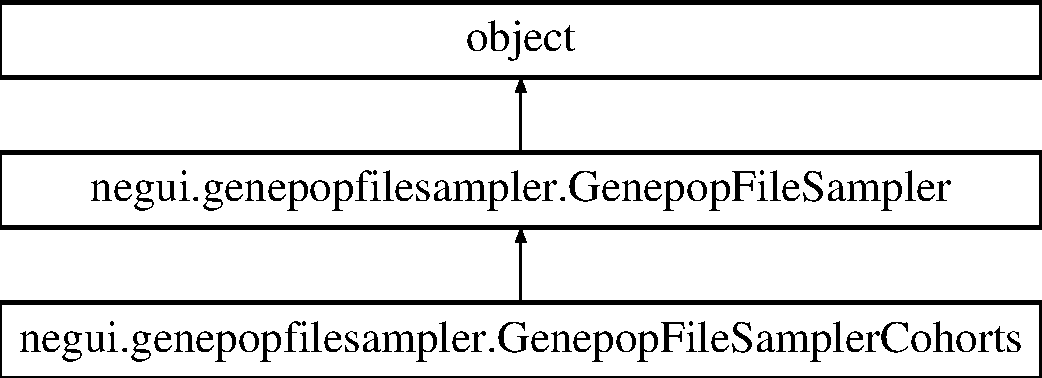
\includegraphics[height=3.000000cm]{classnegui_1_1genepopfilesampler_1_1GenepopFileSamplerCohorts}
\end{center}
\end{figure}
\subsection*{Public Member Functions}
\begin{DoxyCompactItemize}
\item 
def {\bfseries \+\_\+\+\_\+init\+\_\+\+\_\+} (self, o\+\_\+genepopfilemanager, o\+\_\+genepopfilesampleparams)\hypertarget{classnegui_1_1genepopfilesampler_1_1GenepopFileSamplerCohorts_a2b4fa2321a676910d8b11ec2df48fbbf}{}\label{classnegui_1_1genepopfilesampler_1_1GenepopFileSamplerCohorts_a2b4fa2321a676910d8b11ec2df48fbbf}

\item 
def \hyperlink{classnegui_1_1genepopfilesampler_1_1GenepopFileSamplerCohorts_a765e68f8d835bde418cd8c3005b0a97a}{resize\+\_\+sample\+\_\+to\+\_\+meet\+\_\+size\+\_\+criteria} (self, li\+\_\+indiv\+\_\+by\+\_\+age\+\_\+collected)
\item 
def \hyperlink{classnegui_1_1genepopfilesampler_1_1GenepopFileSamplerCohorts_a36977cef305c268768a1ede56ab7fc63}{do\+Sample} (self)
\end{DoxyCompactItemize}


\subsection{Detailed Description}
\begin{DoxyVerb}This sampler class is meant to implement Tiago's sampling code in his
sampleIndivsCohort.py module.  It samples  individuals grouped by age.
The GenepopFileSampleParams object used by instances
of this class has the values Tiagos module takes at the command line 
that restrict the total individuals per gen.  His command line params 
startGen and endGen paramters are already implemented via the Sampler's
li_population_numbers parameter.


2017_07_21.  This class is copied from original version named class
GenepopFileSamplerIndividualsAgeStructureCohorts, and revised to 
handle subsample values using the (new class) GenepopFileSampleParamsCohorts,
which will store lists of proportions and/or indiv count limits.  Further,
this class will use these values (if present) to subsample the already
evenly sampled age classes 0,1...max_age, again, evenly across the age classes.
Note that before this revision, the only subsampling applied (proportion,
via class GenepopFileSamplerIndividualsAgeStructureCohortsPercentage),
sampled a proportion of the pooled age classes, so that the final sample,
if representing multiple age classes, was likely biased towards/against 
one or another across age class).
\end{DoxyVerb}
 

Definition at line 813 of file genepopfilesampler.\+py.



\subsection{Member Function Documentation}
\index{negui\+::genepopfilesampler\+::\+Genepop\+File\+Sampler\+Cohorts@{negui\+::genepopfilesampler\+::\+Genepop\+File\+Sampler\+Cohorts}!do\+Sample@{do\+Sample}}
\index{do\+Sample@{do\+Sample}!negui\+::genepopfilesampler\+::\+Genepop\+File\+Sampler\+Cohorts@{negui\+::genepopfilesampler\+::\+Genepop\+File\+Sampler\+Cohorts}}
\subsubsection[{\texorpdfstring{do\+Sample(self)}{doSample(self)}}]{\setlength{\rightskip}{0pt plus 5cm}def negui.\+genepopfilesampler.\+Genepop\+File\+Sampler\+Cohorts.\+do\+Sample (
\begin{DoxyParamCaption}
\item[{}]{self}
\end{DoxyParamCaption}
)}\hypertarget{classnegui_1_1genepopfilesampler_1_1GenepopFileSamplerCohorts_a36977cef305c268768a1ede56ab7fc63}{}\label{classnegui_1_1genepopfilesampler_1_1GenepopFileSamplerCohorts_a36977cef305c268768a1ede56ab7fc63}
\begin{DoxyVerb}Sample identical numbers per age, then reduce to meet max indiv per gen or proportion.  
See Tiagos code in his sampleIndivsCohort.py module.  Note that when param 
"lp" is included, then Tiagos code adds to his lines that print out, gen_number\sindiv, 
the same lines without a gen number, presumably for downstream filtering when making the final
genenpop file. As of 2016_09_12, the output when the "lp" arg is added, is not 
implemented.

2017_07_21. For this revised version of original class 
GenepopFileSamplerIndividualsAgeStructureCohorts, we use the member of new 
class GenepopFileSampleParamsCohorts, list_of_sampling_values, to loop over
proportion (or count--not yet implemented) subsample values (if any), and 
add a pop subsample tag for each value.  This is an incorporation of the 
original doSample, with the looping logic of the doSample in the original
class GenepopFileSamplerIndividualsAgeStructureCohortsPercentage.
\end{DoxyVerb}
 

Definition at line 972 of file genepopfilesampler.\+py.


\begin{DoxyCode}
972     \textcolor{keyword}{def }\hyperlink{classnegui_1_1genepopfilesampler_1_1GenepopFileSamplerCohorts_a36977cef305c268768a1ede56ab7fc63}{doSample}( self ):
973         \textcolor{stringliteral}{'''}
974 \textcolor{stringliteral}{        Sample identical numbers per age, then reduce to meet max indiv per gen or proportion.  }
975 \textcolor{stringliteral}{        See Tiagos code in his sampleIndivsCohort.py module.  Note that when param }
976 \textcolor{stringliteral}{        "lp" is included, then Tiagos code adds to his lines that print out, gen\_number\(\backslash\)sindiv, }
977 \textcolor{stringliteral}{        the same lines without a gen number, presumably for downstream filtering when making the final}
978 \textcolor{stringliteral}{        genenpop file. As of 2016\_09\_12, the output when the "lp" arg is added, is not }
979 \textcolor{stringliteral}{        implemented.}
980 \textcolor{stringliteral}{}
981 \textcolor{stringliteral}{        2017\_07\_21. For this revised version of original class }
982 \textcolor{stringliteral}{        GenepopFileSamplerIndividualsAgeStructureCohorts, we use the member of new }
983 \textcolor{stringliteral}{        class GenepopFileSampleParamsCohorts, list\_of\_sampling\_values, to loop over}
984 \textcolor{stringliteral}{        proportion (or count--not yet implemented) subsample values (if any), and }
985 \textcolor{stringliteral}{        add a pop subsample tag for each value.  This is an incorporation of the }
986 \textcolor{stringliteral}{        original doSample, with the looping logic of the doSample in the original}
987 \textcolor{stringliteral}{        class GenepopFileSamplerIndividualsAgeStructureCohortsPercentage.}
988 \textcolor{stringliteral}{        '''}
989 
990         \textcolor{comment}{#estimator driver needs a pop number subsample when it adds calls to the NeEstimator:}
991         self.filemanager.subsamplePopulationsByList( self.sampleparams.population\_numbers,
992                                         s\_subsample\_tag=self.sampleparams.population\_subsample\_name )
993 
994         FIELD\_NAME\_AGE=\textcolor{stringliteral}{"age"}
995 
996         \textcolor{stringliteral}{'''}
997 \textcolor{stringliteral}{        If we are processing a session with No }
998 \textcolor{stringliteral}{        subsampling values, we will pass self.\_\_get\_individuals}
999 \textcolor{stringliteral}{        "None"}
1000 \textcolor{stringliteral}{        '''}
1001         lo\_sampling\_value\_objects\_list=[ \textcolor{keywordtype}{None} ]
1002 
1003         \textcolor{keywordflow}{if} self.sampleparams.list\_of\_sampling\_values \textcolor{keywordflow}{is} \textcolor{keywordflow}{not} \textcolor{keywordtype}{None}:
1004             lo\_sampling\_value\_objects\_list=self.sampleparams.list\_of\_sampling\_values
1005         \textcolor{comment}{#end if no samping value (i.e. schem is "none") else we have them}
1006 
1007         \textcolor{keywordflow}{for} o\_sampling\_value\_object \textcolor{keywordflow}{in} lo\_sampling\_value\_objects\_list:
1008             
1009             dli\_indiv\_index\_lists\_by\_pop\_number=\{\}
1010             
1011             i\_replicate\_count=self.sampleparams.replicates
1012 
1013             \textcolor{keywordflow}{for} i\_replicate\_number \textcolor{keywordflow}{in} range( i\_replicate\_count ):
1014 
1015                 \textcolor{keywordflow}{for} i\_pop\_number \textcolor{keywordflow}{in} self.sampleparams.population\_numbers:
1016 
1017                     ls\_id\_list=self.filemanager.getListIndividuals( i\_pop\_number )
1018 
1019                     \textcolor{stringliteral}{'''}
1020 \textcolor{stringliteral}{                    We assume that the list of Id's in the individual list}
1021 \textcolor{stringliteral}{                    is indexed such that the zeroth id corresponds to the first}
1022 \textcolor{stringliteral}{                    indiv as ordered in the genepop file, the [1] indexed id}
1023 \textcolor{stringliteral}{                    is the second indiv, etc.}
1024 \textcolor{stringliteral}{                    '''}
1025                     i\_tot\_indiv=len( ls\_id\_list )
1026 
1027                     dli\_indiv\_index\_by\_age=\{\}
1028                     
1029                     \textcolor{keywordflow}{for} idx \textcolor{keywordflow}{in} range( i\_tot\_indiv ):
1030 
1031                         s\_id=ls\_id\_list[ idx ]
1032 
1033                         o\_id\_vals=GenepopIndivIdVals( s\_id, 
1034                                             self.sampleparams.fields )
1035                         
1036                         \textcolor{comment}{#age may be float or int:}
1037                         v\_age=o\_id\_vals.getVal( FIELD\_NAME\_AGE )
1038 
1039                         \textcolor{keywordflow}{if} v\_age > self.sampleparams.max\_age:
1040                             \textcolor{keywordflow}{continue}
1041                         \textcolor{comment}{#end if too old, continue}
1042 
1043                         \textcolor{stringliteral}{'''}
1044 \textcolor{stringliteral}{                        Note that idx+1 gives the number of the individual as ordered by its}
1045 \textcolor{stringliteral}{                        entry in the "pop" section of this pop in the genepop file, as used}
1046 \textcolor{stringliteral}{                        by the genepopfilemanager object to point to it's byte address in the file.}
1047 \textcolor{stringliteral}{                        Thus it's our way of collecting samples of individuals and passing them into the}
1048 \textcolor{stringliteral}{                        genepop file manager object's subsampling records (its attribute }
1049 \textcolor{stringliteral}{                        \_\_indiv\_subsamples).}
1050 \textcolor{stringliteral}{                        '''}
1051 
1052                         i\_indiv\_number=idx+1
1053 
1054                         dli\_indiv\_index\_by\_age.setdefault( \(\backslash\)
1055                                     v\_age, [] ).append( i\_indiv\_number ) 
1056 
1057                     \textcolor{comment}{#end for each individual's id   }
1058 
1059                     li\_indiv\_by\_age\_collected=self.\hyperlink{classnegui_1_1genepopfilesampler_1_1GenepopFileSamplerCohorts_a1b370307615aa6267a6f287180030058}{\_\_get\_individuals}( \(\backslash\)
1060                                                     dli\_indiv\_index\_by\_age,
1061                                                     o\_sampling\_value\_object ) 
1062                 
1063                     \textcolor{stringliteral}{'''}
1064 \textcolor{stringliteral}{                    2017\_07\_21.  We note that, for now, this call will simply throw }
1065 \textcolor{stringliteral}{                    an error if the current sample (pooled individuals from all age classes,}
1066 \textcolor{stringliteral}{                    with any proportion or count subsample value also applied,}
1067 \textcolor{stringliteral}{                    '''}
1068                     li\_indiv\_by\_age\_sampled=self.
      \hyperlink{classnegui_1_1genepopfilesampler_1_1GenepopFileSamplerCohorts_a765e68f8d835bde418cd8c3005b0a97a}{resize\_sample\_to\_meet\_size\_criteria}( 
1069                                                                 li\_indiv\_by\_age\_collected ) 
1070 
1071                     \textcolor{comment}{#We rely on the genpopfilemanager object to sort }
1072                     \textcolor{comment}{#these indices when we pass them to the def,}
1073                     \textcolor{comment}{#subsampleIndividualsByNumberList (see below).}
1074                     dli\_indiv\_index\_lists\_by\_pop\_number[ i\_pop\_number ] = \(\backslash\)
1075                                                         li\_indiv\_by\_age\_sampled
1076                 \textcolor{comment}{#end for each pop number}
1077 
1078                 \textcolor{keywordflow}{if} o\_sampling\_value\_object \textcolor{keywordflow}{is} \textcolor{keywordflow}{not} \textcolor{keywordtype}{None}:
1079                     self.sampleparams.sample\_param\_value=\(\backslash\)
1080                             str( o\_sampling\_value\_object.sampling\_value )
1081                 \textcolor{comment}{#end if we have a sampling value}
1082                 
1083                 s\_this\_subsample\_name=make\_subsample\_tag( \(\backslash\)
1084                                     self.sampleparams.sample\_param\_value, 
1085                                     i\_replicate\_number, 
1086                                     SCHEME\_COHORTS,
1087                                     s\_prefix=self.sampleparams.sample\_tag\_base )
1088                 
1089                 self.filemanager.subsampleIndividualsByNumberList( \(\backslash\)
1090                                         dli\_indiv\_index\_lists\_by\_pop\_number,
1091                                         s\_this\_subsample\_name )
1092             \textcolor{comment}{#end for each replicate}
1093         \textcolor{comment}{#end for each  sampling value}
1094         \textcolor{keywordflow}{return}
\end{DoxyCode}
\index{negui\+::genepopfilesampler\+::\+Genepop\+File\+Sampler\+Cohorts@{negui\+::genepopfilesampler\+::\+Genepop\+File\+Sampler\+Cohorts}!resize\+\_\+sample\+\_\+to\+\_\+meet\+\_\+size\+\_\+criteria@{resize\+\_\+sample\+\_\+to\+\_\+meet\+\_\+size\+\_\+criteria}}
\index{resize\+\_\+sample\+\_\+to\+\_\+meet\+\_\+size\+\_\+criteria@{resize\+\_\+sample\+\_\+to\+\_\+meet\+\_\+size\+\_\+criteria}!negui\+::genepopfilesampler\+::\+Genepop\+File\+Sampler\+Cohorts@{negui\+::genepopfilesampler\+::\+Genepop\+File\+Sampler\+Cohorts}}
\subsubsection[{\texorpdfstring{resize\+\_\+sample\+\_\+to\+\_\+meet\+\_\+size\+\_\+criteria(self, li\+\_\+indiv\+\_\+by\+\_\+age\+\_\+collected)}{resize_sample_to_meet_size_criteria(self, li_indiv_by_age_collected)}}]{\setlength{\rightskip}{0pt plus 5cm}def negui.\+genepopfilesampler.\+Genepop\+File\+Sampler\+Cohorts.\+resize\+\_\+sample\+\_\+to\+\_\+meet\+\_\+size\+\_\+criteria (
\begin{DoxyParamCaption}
\item[{}]{self, }
\item[{}]{li\+\_\+indiv\+\_\+by\+\_\+age\+\_\+collected}
\end{DoxyParamCaption}
)}\hypertarget{classnegui_1_1genepopfilesampler_1_1GenepopFileSamplerCohorts_a765e68f8d835bde418cd8c3005b0a97a}{}\label{classnegui_1_1genepopfilesampler_1_1GenepopFileSamplerCohorts_a765e68f8d835bde418cd8c3005b0a97a}
\begin{DoxyVerb}Given the individuals collected by age, 
check min/max limits and subsample
if needed.  If within limits, return
the original list
\end{DoxyVerb}
 

Definition at line 921 of file genepopfilesampler.\+py.


\begin{DoxyCode}
921     \textcolor{keyword}{def }\hyperlink{classnegui_1_1genepopfilesampler_1_1GenepopFileSamplerCohorts_a765e68f8d835bde418cd8c3005b0a97a}{resize\_sample\_to\_meet\_size\_criteria}( self, 
      li\_indiv\_by\_age\_collected ):
922         \textcolor{stringliteral}{'''}
923 \textcolor{stringliteral}{        Given the individuals collected by age, }
924 \textcolor{stringliteral}{        check min/max limits and subsample}
925 \textcolor{stringliteral}{        if needed.  If within limits, return}
926 \textcolor{stringliteral}{        the original list}
927 \textcolor{stringliteral}{        '''}
928 
929         \textcolor{comment}{#If too few we raise an error.  If too many we}
930         \textcolor{comment}{#randomly select to reach our max valid pop size}
931         i\_tot\_collected=len( li\_indiv\_by\_age\_collected )
932 
933         li\_indiv\_by\_age\_sampled=\textcolor{keywordtype}{None}
934 
935         \textcolor{keywordflow}{if} i\_tot\_collected < self.sampleparams.min\_indiv\_per\_gen:
936             s\_msg=\textcolor{stringliteral}{"In GenepopFileSamplerIndividualsAgeStructureCohorts instance, "} \(\backslash\)
937                     \textcolor{stringliteral}{"after sampling cohorts, total collected, "} \(\backslash\)
938                     + str( i\_tot\_collected ) \(\backslash\)
939                     + \textcolor{stringliteral}{", is less than the value given for "} \(\backslash\)
940                     + \textcolor{stringliteral}{"the minimum pop size, "} \(\backslash\)
941                     + str( self.sampleparams.min\_indiv\_per\_gen ) \(\backslash\)
942                     + \textcolor{stringliteral}{"."}
943             \textcolor{keywordflow}{raise} Exception ( s\_msg )
944 
945         \textcolor{keywordflow}{elif} i\_tot\_collected > self.sampleparams.max\_indiv\_per\_gen:
946             \textcolor{keywordflow}{try}:
947 
948                 li\_indiv\_by\_age\_sampled=random.sample( \(\backslash\)
949                                     li\_indiv\_by\_age\_collected,
950                                     self.sampleparams.max\_indiv\_per\_gen )
951                                         
952             \textcolor{keywordflow}{except} Exception \textcolor{keyword}{as} oex:
953                 s\_sample\_error\_msg= \(\backslash\)
954                     \textcolor{stringliteral}{"In GenepopFileSamplerIndividualsAgeStructureCohorts "} \(\backslash\)
955                         + \textcolor{stringliteral}{"instance, def resize\_sample\_to\_meet\_size\_criteria, "}  \(\backslash\)
956                         + \textcolor{stringliteral}{"random.sample failed on list of "} \(\backslash\)
957                         + str( len( li\_indiv\_by\_age\_collected ) ) \(\backslash\)
958                         + \textcolor{stringliteral}{" individuals.  Target total to be sampled: "} \(\backslash\)
959                         + str( self.sampleparams.max\_indiv\_per\_gen ) + \textcolor{stringliteral}{"."}
960                 s\_msg=s\_sample\_error\_msg \(\backslash\)
961                         + \textcolor{stringliteral}{"  Exception message: "} + str( oex ) + \textcolor{stringliteral}{"."}
962                 \textcolor{keywordflow}{raise} Exception( s\_msg )
963             \textcolor{comment}{#end try . . . except}
964         \textcolor{keywordflow}{else}:
965             \textcolor{comment}{#within interval min to max pop size, so keep original }
966             li\_indiv\_by\_age\_sampled=li\_indiv\_by\_age\_collected
967 
968         \textcolor{comment}{#end if too few, error, else if too many, sample, else no change}
969         \textcolor{keywordflow}{return} li\_indiv\_by\_age\_sampled
\end{DoxyCode}


The documentation for this class was generated from the following file\+:\begin{DoxyCompactItemize}
\item 
genepopfilesampler.\+py\end{DoxyCompactItemize}

\hypertarget{classnegui_1_1genepopfilesampler_1_1GenepopFileSamplerIndividualsAgeStructureCohorts}{}\section{negui.\+genepopfilesampler.\+Genepop\+File\+Sampler\+Individuals\+Age\+Structure\+Cohorts Class Reference}
\label{classnegui_1_1genepopfilesampler_1_1GenepopFileSamplerIndividualsAgeStructureCohorts}\index{negui.\+genepopfilesampler.\+Genepop\+File\+Sampler\+Individuals\+Age\+Structure\+Cohorts@{negui.\+genepopfilesampler.\+Genepop\+File\+Sampler\+Individuals\+Age\+Structure\+Cohorts}}
Inheritance diagram for negui.\+genepopfilesampler.\+Genepop\+File\+Sampler\+Individuals\+Age\+Structure\+Cohorts\+:\begin{figure}[H]
\begin{center}
\leavevmode
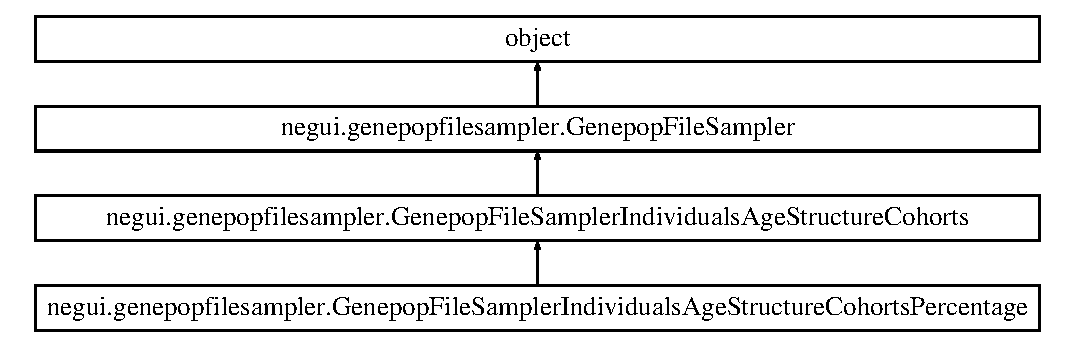
\includegraphics[height=4.000000cm]{classnegui_1_1genepopfilesampler_1_1GenepopFileSamplerIndividualsAgeStructureCohorts}
\end{center}
\end{figure}
\subsection*{Public Member Functions}
\begin{DoxyCompactItemize}
\item 
def {\bfseries \+\_\+\+\_\+init\+\_\+\+\_\+} (self, o\+\_\+genepopfilemanager, o\+\_\+genepopfilesampleparams)\hypertarget{classnegui_1_1genepopfilesampler_1_1GenepopFileSamplerIndividualsAgeStructureCohorts_ab997e641e99278377a07624ad847a697}{}\label{classnegui_1_1genepopfilesampler_1_1GenepopFileSamplerIndividualsAgeStructureCohorts_ab997e641e99278377a07624ad847a697}

\item 
def \hyperlink{classnegui_1_1genepopfilesampler_1_1GenepopFileSamplerIndividualsAgeStructureCohorts_a28deaac6347b19f565b2a50f233a6f06}{resize\+\_\+sample\+\_\+to\+\_\+meet\+\_\+size\+\_\+criteria} (self, li\+\_\+indiv\+\_\+by\+\_\+age\+\_\+collected)
\item 
def \hyperlink{classnegui_1_1genepopfilesampler_1_1GenepopFileSamplerIndividualsAgeStructureCohorts_a50e96ddae763e7e8dba2ac37fa0c6ce5}{do\+Sample} (self)
\end{DoxyCompactItemize}


\subsection{Detailed Description}
\begin{DoxyVerb}This sampler class is meant to implement Tiago's sampling code in his
sampleIndivsCohort.py module.  It samples  individuals grouped by age.
The GenepopFileSampleParams object used by instances
of this class has the values Tiagos module takes at the command line 
that restrict the total individuals per gen.  His command line params 
startGen and endGen paramters are already implemented via the Sampler's
li_population_numbers parameter.
\end{DoxyVerb}
 

Definition at line 1103 of file genepopfilesampler.\+py.



\subsection{Member Function Documentation}
\index{negui\+::genepopfilesampler\+::\+Genepop\+File\+Sampler\+Individuals\+Age\+Structure\+Cohorts@{negui\+::genepopfilesampler\+::\+Genepop\+File\+Sampler\+Individuals\+Age\+Structure\+Cohorts}!do\+Sample@{do\+Sample}}
\index{do\+Sample@{do\+Sample}!negui\+::genepopfilesampler\+::\+Genepop\+File\+Sampler\+Individuals\+Age\+Structure\+Cohorts@{negui\+::genepopfilesampler\+::\+Genepop\+File\+Sampler\+Individuals\+Age\+Structure\+Cohorts}}
\subsubsection[{\texorpdfstring{do\+Sample(self)}{doSample(self)}}]{\setlength{\rightskip}{0pt plus 5cm}def negui.\+genepopfilesampler.\+Genepop\+File\+Sampler\+Individuals\+Age\+Structure\+Cohorts.\+do\+Sample (
\begin{DoxyParamCaption}
\item[{}]{self}
\end{DoxyParamCaption}
)}\hypertarget{classnegui_1_1genepopfilesampler_1_1GenepopFileSamplerIndividualsAgeStructureCohorts_a50e96ddae763e7e8dba2ac37fa0c6ce5}{}\label{classnegui_1_1genepopfilesampler_1_1GenepopFileSamplerIndividualsAgeStructureCohorts_a50e96ddae763e7e8dba2ac37fa0c6ce5}
\begin{DoxyVerb}Sample identical numbers per age, then reduce to meet max indiv per gen or proportion.  
See Tiagos code in his sampleIndivsCohort.py module.  Note that when param "lp" is 
included, then Tiagos code adds to his lines that print out, gen_number\sindiv, the same lines
without a gen number, presumably for downstream filtering when making the final
genenpop file. As of 2016_09_12, the output when the "lp" arg is added, is not 
implemented.
\end{DoxyVerb}
 

Definition at line 1197 of file genepopfilesampler.\+py.


\begin{DoxyCode}
1197     \textcolor{keyword}{def }\hyperlink{classnegui_1_1genepopfilesampler_1_1GenepopFileSamplerIndividualsAgeStructureCohorts_a50e96ddae763e7e8dba2ac37fa0c6ce5}{doSample}( self ):
1198         \textcolor{stringliteral}{'''}
1199 \textcolor{stringliteral}{        Sample identical numbers per age, then reduce to meet max indiv per gen or proportion.  }
1200 \textcolor{stringliteral}{        See Tiagos code in his sampleIndivsCohort.py module.  Note that when param "lp" is }
1201 \textcolor{stringliteral}{        included, then Tiagos code adds to his lines that print out, gen\_number\(\backslash\)sindiv, the same lines}
1202 \textcolor{stringliteral}{        without a gen number, presumably for downstream filtering when making the final}
1203 \textcolor{stringliteral}{        genenpop file. As of 2016\_09\_12, the output when the "lp" arg is added, is not }
1204 \textcolor{stringliteral}{        implemented.}
1205 \textcolor{stringliteral}{        '''}
1206 
1207         \textcolor{comment}{#estimator driver needs a pop number subsample when it adds calls to the NeEstimator:}
1208         self.filemanager.subsamplePopulationsByList( self.sampleparams.population\_numbers,
1209                                         s\_subsample\_tag=self.sampleparams.population\_subsample\_name )
1210 
1211         FIELD\_NAME\_AGE=\textcolor{stringliteral}{"age"}
1212 
1213         dli\_indiv\_index\_lists\_by\_pop\_number=\{\}
1214         
1215         i\_replicate\_count=self.sampleparams.replicates
1216 
1217         \textcolor{keywordflow}{for} i\_replicate\_number \textcolor{keywordflow}{in} range( i\_replicate\_count ):
1218 
1219             \textcolor{keywordflow}{for} i\_pop\_number \textcolor{keywordflow}{in} self.sampleparams.population\_numbers:
1220 
1221                 ls\_id\_list=self.filemanager.getListIndividuals( i\_pop\_number )
1222 
1223                 \textcolor{stringliteral}{'''}
1224 \textcolor{stringliteral}{                We assume that the list of Id's in the individual list}
1225 \textcolor{stringliteral}{                is indexed such that the zeroth id corresponds to the first}
1226 \textcolor{stringliteral}{                indiv as ordered in the genepop file, the [1] indexed id}
1227 \textcolor{stringliteral}{                is the second indiv, etc.}
1228 \textcolor{stringliteral}{                '''}
1229                 i\_tot\_indiv=len( ls\_id\_list )
1230 
1231                 dli\_indiv\_index\_by\_age=\{\}
1232                 
1233                 \textcolor{keywordflow}{for} idx \textcolor{keywordflow}{in} range( i\_tot\_indiv ):
1234 
1235                     s\_id=ls\_id\_list[ idx ]
1236 
1237                     o\_id\_vals=GenepopIndivIdVals( s\_id, 
1238                                         self.sampleparams.fields )
1239                     
1240                     \textcolor{comment}{#age may be float or int:}
1241                     v\_age=o\_id\_vals.getVal( FIELD\_NAME\_AGE )
1242 
1243                     \textcolor{keywordflow}{if} v\_age > self.sampleparams.max\_age:
1244                         \textcolor{keywordflow}{continue}
1245                     \textcolor{comment}{#end if too old, continue}
1246 
1247                     \textcolor{stringliteral}{'''}
1248 \textcolor{stringliteral}{                    Note that idx+1 gives the number of the individual as ordered by its}
1249 \textcolor{stringliteral}{                    entry in the "pop" section of this pop in the genepop file, as used}
1250 \textcolor{stringliteral}{                    by the genepopfilemanager object to point to it's byte address in the file.}
1251 \textcolor{stringliteral}{                    Thus it's our way of collecting samples of individuals and passing them into the}
1252 \textcolor{stringliteral}{                    genepop file manager object's subsampling records (its attribute }
1253 \textcolor{stringliteral}{                    \_\_indiv\_subsamples).}
1254 \textcolor{stringliteral}{                    '''}
1255 
1256                     i\_indiv\_number=idx+1
1257 
1258                     dli\_indiv\_index\_by\_age.setdefault( \(\backslash\)
1259                                 v\_age, [] ).append( i\_indiv\_number ) 
1260 
1261                 \textcolor{comment}{#end for each individual's id   }
1262 
1263                 li\_indiv\_by\_age\_collected=self.\hyperlink{classnegui_1_1genepopfilesampler_1_1GenepopFileSamplerIndividualsAgeStructureCohorts_a7c5c9e3e3aeb9c9c25c95029781e63d1}{\_\_get\_individuals}( \(\backslash\)
1264                                                 dli\_indiv\_index\_by\_age ) 
1265             
1266                 \textcolor{stringliteral}{'''}
1267 \textcolor{stringliteral}{                Resize the sample if it exceeds size limits (as given by}
1268 \textcolor{stringliteral}{                min,max, or, in the case of a proportionaly sampling scheme}
1269 \textcolor{stringliteral}{                (subclass GenepopFileSamplerIndividualsAgeStructureCohortsPercentage),}
1270 \textcolor{stringliteral}{                subsample a proportion.  Note that these lists will be sorted by the}
1271 \textcolor{stringliteral}{                GenepopFileManager in the subsampleIndividualsByNumberList call}
1272 \textcolor{stringliteral}{                below.}
1273 \textcolor{stringliteral}{                '''}
1274 
1275                 li\_indiv\_by\_age\_sampled=self.\hyperlink{classnegui_1_1genepopfilesampler_1_1GenepopFileSamplerIndividualsAgeStructureCohorts_a28deaac6347b19f565b2a50f233a6f06}{resize\_sample\_to\_meet\_size\_criteria}
      ( 
1276                                                             li\_indiv\_by\_age\_collected ) 
1277 
1278 
1279                 \textcolor{comment}{#We rely on the genpopfilemanager object to sort }
1280                 \textcolor{comment}{#these indices when we pass them to the def,}
1281                 \textcolor{comment}{#subsampleIndividualsByNumberList (see below).}
1282                 dli\_indiv\_index\_lists\_by\_pop\_number[ i\_pop\_number ] = \(\backslash\)
1283                                                     li\_indiv\_by\_age\_sampled
1284             \textcolor{comment}{#end for each pop number}
1285             
1286             s\_this\_subsample\_name=make\_subsample\_tag( \(\backslash\)
1287                                 self.sampleparams.sample\_param\_value, 
1288                                 i\_replicate\_number, 
1289                                 SCHEME\_COHORTS,
1290                                 s\_prefix=self.sampleparams.sample\_tag\_base )
1291             
1292             self.filemanager.subsampleIndividualsByNumberList( \(\backslash\)
1293                                     dli\_indiv\_index\_lists\_by\_pop\_number,
1294                                     s\_this\_subsample\_name )
1295 
1296         \textcolor{comment}{#end for each replicate}
1297         \textcolor{keywordflow}{return}
\end{DoxyCode}
\index{negui\+::genepopfilesampler\+::\+Genepop\+File\+Sampler\+Individuals\+Age\+Structure\+Cohorts@{negui\+::genepopfilesampler\+::\+Genepop\+File\+Sampler\+Individuals\+Age\+Structure\+Cohorts}!resize\+\_\+sample\+\_\+to\+\_\+meet\+\_\+size\+\_\+criteria@{resize\+\_\+sample\+\_\+to\+\_\+meet\+\_\+size\+\_\+criteria}}
\index{resize\+\_\+sample\+\_\+to\+\_\+meet\+\_\+size\+\_\+criteria@{resize\+\_\+sample\+\_\+to\+\_\+meet\+\_\+size\+\_\+criteria}!negui\+::genepopfilesampler\+::\+Genepop\+File\+Sampler\+Individuals\+Age\+Structure\+Cohorts@{negui\+::genepopfilesampler\+::\+Genepop\+File\+Sampler\+Individuals\+Age\+Structure\+Cohorts}}
\subsubsection[{\texorpdfstring{resize\+\_\+sample\+\_\+to\+\_\+meet\+\_\+size\+\_\+criteria(self, li\+\_\+indiv\+\_\+by\+\_\+age\+\_\+collected)}{resize_sample_to_meet_size_criteria(self, li_indiv_by_age_collected)}}]{\setlength{\rightskip}{0pt plus 5cm}def negui.\+genepopfilesampler.\+Genepop\+File\+Sampler\+Individuals\+Age\+Structure\+Cohorts.\+resize\+\_\+sample\+\_\+to\+\_\+meet\+\_\+size\+\_\+criteria (
\begin{DoxyParamCaption}
\item[{}]{self, }
\item[{}]{li\+\_\+indiv\+\_\+by\+\_\+age\+\_\+collected}
\end{DoxyParamCaption}
)}\hypertarget{classnegui_1_1genepopfilesampler_1_1GenepopFileSamplerIndividualsAgeStructureCohorts_a28deaac6347b19f565b2a50f233a6f06}{}\label{classnegui_1_1genepopfilesampler_1_1GenepopFileSamplerIndividualsAgeStructureCohorts_a28deaac6347b19f565b2a50f233a6f06}
\begin{DoxyVerb}Given the individuals collected by age, 
check min/max limits and subsample
if needed.  If within limits, return
the original list
\end{DoxyVerb}
 

Definition at line 1146 of file genepopfilesampler.\+py.


\begin{DoxyCode}
1146     \textcolor{keyword}{def }\hyperlink{classnegui_1_1genepopfilesampler_1_1GenepopFileSamplerIndividualsAgeStructureCohorts_a28deaac6347b19f565b2a50f233a6f06}{resize\_sample\_to\_meet\_size\_criteria}( self, 
      li\_indiv\_by\_age\_collected ):
1147         \textcolor{stringliteral}{'''}
1148 \textcolor{stringliteral}{        Given the individuals collected by age, }
1149 \textcolor{stringliteral}{        check min/max limits and subsample}
1150 \textcolor{stringliteral}{        if needed.  If within limits, return}
1151 \textcolor{stringliteral}{        the original list}
1152 \textcolor{stringliteral}{        '''}
1153 
1154         \textcolor{comment}{#If too few we raise an error.  If too many we}
1155         \textcolor{comment}{#randomly select to reach our max valid pop size}
1156         i\_tot\_collected=len( li\_indiv\_by\_age\_collected )
1157 
1158         li\_indiv\_by\_age\_sampled=\textcolor{keywordtype}{None}
1159 
1160         \textcolor{keywordflow}{if} i\_tot\_collected < self.sampleparams.min\_indiv\_per\_gen:
1161             s\_msg=\textcolor{stringliteral}{"In GenepopFileSamplerIndividualsAgeStructureCohorts instance, "} \(\backslash\)
1162                     \textcolor{stringliteral}{"after sampling cohorts, total collected, "} \(\backslash\)
1163                     + str( i\_tot\_collected ) \(\backslash\)
1164                     + \textcolor{stringliteral}{", is less than the value given for "} \(\backslash\)
1165                     + \textcolor{stringliteral}{"the minimum pop size, "} \(\backslash\)
1166                     + str( self.sampleparams.min\_indiv\_per\_gen ) \(\backslash\)
1167                     + \textcolor{stringliteral}{"."}
1168             \textcolor{keywordflow}{raise} Exception ( s\_msg )
1169 
1170         \textcolor{keywordflow}{elif} i\_tot\_collected > self.sampleparams.max\_indiv\_per\_gen:
1171             \textcolor{keywordflow}{try}:
1172 
1173                 li\_indiv\_by\_age\_sampled=random.sample( \(\backslash\)
1174                                     li\_indiv\_by\_age\_collected,
1175                                     self.sampleparams.max\_indiv\_per\_gen )
1176                                         
1177             \textcolor{keywordflow}{except} Exception \textcolor{keyword}{as} oex:
1178                 s\_sample\_error\_msg= \(\backslash\)
1179                     \textcolor{stringliteral}{"In GenepopFileSamplerIndividualsAgeStructureCohorts "} \(\backslash\)
1180                         + \textcolor{stringliteral}{"instance, def resize\_sample\_to\_meet\_size\_criteria, "}  \(\backslash\)
1181                         + \textcolor{stringliteral}{"random.sample failed on list of "} \(\backslash\)
1182                         + str( len( li\_indiv\_by\_age\_collected ) ) \(\backslash\)
1183                         + \textcolor{stringliteral}{" individuals.  Target total to be sampled: "} \(\backslash\)
1184                         + str( self.sampleparams.max\_indiv\_per\_gen ) + \textcolor{stringliteral}{"."}
1185                 s\_msg=s\_sample\_error\_msg \(\backslash\)
1186                         + \textcolor{stringliteral}{"  Exception message: "} + str( oex ) + \textcolor{stringliteral}{"."}
1187                 \textcolor{keywordflow}{raise} Exception( s\_msg )
1188             \textcolor{comment}{#end try . . . except}
1189         \textcolor{keywordflow}{else}:
1190             \textcolor{comment}{#within interval min to max pop size, so keep original }
1191             li\_indiv\_by\_age\_sampled=li\_indiv\_by\_age\_collected
1192 
1193         \textcolor{comment}{#end if too few, error, else if too many, sample, else no change}
1194         \textcolor{keywordflow}{return} li\_indiv\_by\_age\_sampled
\end{DoxyCode}


The documentation for this class was generated from the following file\+:\begin{DoxyCompactItemize}
\item 
genepopfilesampler.\+py\end{DoxyCompactItemize}

\hypertarget{classnegui_1_1genepopfilesampler_1_1GenepopFileSamplerIndividualsAgeStructureCohortsPercentage}{}\section{negui.\+genepopfilesampler.\+Genepop\+File\+Sampler\+Individuals\+Age\+Structure\+Cohorts\+Percentage Class Reference}
\label{classnegui_1_1genepopfilesampler_1_1GenepopFileSamplerIndividualsAgeStructureCohortsPercentage}\index{negui.\+genepopfilesampler.\+Genepop\+File\+Sampler\+Individuals\+Age\+Structure\+Cohorts\+Percentage@{negui.\+genepopfilesampler.\+Genepop\+File\+Sampler\+Individuals\+Age\+Structure\+Cohorts\+Percentage}}
Inheritance diagram for negui.\+genepopfilesampler.\+Genepop\+File\+Sampler\+Individuals\+Age\+Structure\+Cohorts\+Percentage\+:\begin{figure}[H]
\begin{center}
\leavevmode
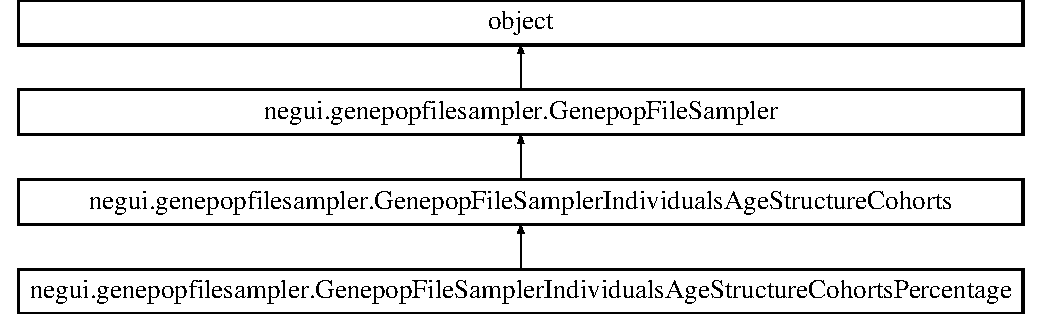
\includegraphics[height=4.000000cm]{classnegui_1_1genepopfilesampler_1_1GenepopFileSamplerIndividualsAgeStructureCohortsPercentage}
\end{center}
\end{figure}
\subsection*{Public Member Functions}
\begin{DoxyCompactItemize}
\item 
def {\bfseries \+\_\+\+\_\+init\+\_\+\+\_\+} (self, o\+\_\+genepopfilemanager, o\+\_\+genepopfilesampleparams)\hypertarget{classnegui_1_1genepopfilesampler_1_1GenepopFileSamplerIndividualsAgeStructureCohortsPercentage_a70a4ae2ec84f02b164b34c741b09c34b}{}\label{classnegui_1_1genepopfilesampler_1_1GenepopFileSamplerIndividualsAgeStructureCohortsPercentage_a70a4ae2ec84f02b164b34c741b09c34b}

\item 
def \hyperlink{classnegui_1_1genepopfilesampler_1_1GenepopFileSamplerIndividualsAgeStructureCohortsPercentage_a84ae04a169f95a289b6aacc21db39a17}{resize\+\_\+sample\+\_\+to\+\_\+meet\+\_\+size\+\_\+criteria} (self, li\+\_\+indiv\+\_\+by\+\_\+age\+\_\+collected)
\item 
def \hyperlink{classnegui_1_1genepopfilesampler_1_1GenepopFileSamplerIndividualsAgeStructureCohortsPercentage_a295926d11ecac7194c52615902bdaf3c}{do\+Sample} (self)
\end{DoxyCompactItemize}


\subsection{Detailed Description}
\begin{DoxyVerb}Sublcass of GenepopFileSamplerIndividualsAgeStructureCohorts.  The only revision
fo the parent class is in def resize_sample_to_meet_size_criteria.  For this
subclass we use the proportion attribute to subsample, whereas in the parent
class we apply max indiv per pop.
\end{DoxyVerb}
 

Definition at line 1302 of file genepopfilesampler.\+py.



\subsection{Member Function Documentation}
\index{negui\+::genepopfilesampler\+::\+Genepop\+File\+Sampler\+Individuals\+Age\+Structure\+Cohorts\+Percentage@{negui\+::genepopfilesampler\+::\+Genepop\+File\+Sampler\+Individuals\+Age\+Structure\+Cohorts\+Percentage}!do\+Sample@{do\+Sample}}
\index{do\+Sample@{do\+Sample}!negui\+::genepopfilesampler\+::\+Genepop\+File\+Sampler\+Individuals\+Age\+Structure\+Cohorts\+Percentage@{negui\+::genepopfilesampler\+::\+Genepop\+File\+Sampler\+Individuals\+Age\+Structure\+Cohorts\+Percentage}}
\subsubsection[{\texorpdfstring{do\+Sample(self)}{doSample(self)}}]{\setlength{\rightskip}{0pt plus 5cm}def negui.\+genepopfilesampler.\+Genepop\+File\+Sampler\+Individuals\+Age\+Structure\+Cohorts\+Percentage.\+do\+Sample (
\begin{DoxyParamCaption}
\item[{}]{self}
\end{DoxyParamCaption}
)}\hypertarget{classnegui_1_1genepopfilesampler_1_1GenepopFileSamplerIndividualsAgeStructureCohortsPercentage_a295926d11ecac7194c52615902bdaf3c}{}\label{classnegui_1_1genepopfilesampler_1_1GenepopFileSamplerIndividualsAgeStructureCohortsPercentage_a295926d11ecac7194c52615902bdaf3c}
\begin{DoxyVerb}This override of the parent class doSample def
iterates over the param list of proportions, 
for each proportion value it sets member __current_param
accordingly, and then calls the parent doSample.  This 
latter will then, after collecting cohorts per max age,
then call the overridden def resize_sample_to_meet_size_criteria, 
which will sample at the "__current_param" proportion.
\end{DoxyVerb}
 

Definition at line 1393 of file genepopfilesampler.\+py.


\begin{DoxyCode}
1393     \textcolor{keyword}{def }\hyperlink{classnegui_1_1genepopfilesampler_1_1GenepopFileSamplerIndividualsAgeStructureCohortsPercentage_a295926d11ecac7194c52615902bdaf3c}{doSample}( self ):
1394         \textcolor{stringliteral}{'''}
1395 \textcolor{stringliteral}{        This override of the parent class doSample def}
1396 \textcolor{stringliteral}{        iterates over the param list of proportions, }
1397 \textcolor{stringliteral}{        for each proportion value it sets member \_\_current\_param}
1398 \textcolor{stringliteral}{        accordingly, and then calls the parent doSample.  This }
1399 \textcolor{stringliteral}{        latter will then, after collecting cohorts per max age,}
1400 \textcolor{stringliteral}{        then call the overridden def resize\_sample\_to\_meet\_size\_criteria, }
1401 \textcolor{stringliteral}{        which will sample at the "\_\_current\_param" proportion.}
1402 \textcolor{stringliteral}{        '''}
1403         \textcolor{keywordflow}{for} f\_proportion \textcolor{keywordflow}{in} self.sampleparams.proportions:
1404 
1405             \textcolor{stringliteral}{'''}
1406 \textcolor{stringliteral}{            When the parent class calls the resize\_sample\_to\_meet\_size\_criteria}
1407 \textcolor{stringliteral}{            def, this derived classe's version will use this}
1408 \textcolor{stringliteral}{            value to sample the pop, after parent applies the}
1409 \textcolor{stringliteral}{            age filter:}
1410 \textcolor{stringliteral}{            '''}
1411             self.\hyperlink{classnegui_1_1genepopfilesampler_1_1GenepopFileSamplerIndividualsAgeStructureCohortsPercentage_a20c7fca4ce503d025b2728ee416b1d6a}{\_\_current\_proportion}=f\_proportion
1412 
1413             \textcolor{comment}{#When the parent class calls def, make\_subsample\_tag, it}
1414             \textcolor{comment}{#will find this value in the sampleparams:}
1415             self.sampleparams.sample\_param\_value=f\_proportion 
1416 
1417             super( GenepopFileSamplerIndividualsAgeStructureCohortsPercentage, self ).
      \hyperlink{classnegui_1_1genepopfilesampler_1_1GenepopFileSamplerIndividualsAgeStructureCohortsPercentage_a295926d11ecac7194c52615902bdaf3c}{doSample}()
1418         \textcolor{comment}{#end for each proportion}
1419         \textcolor{keywordflow}{return}
1420 \textcolor{comment}{#end class GenepopFileSamplerIndividualsAgeStructureCohortsPercentage}
1421 
\end{DoxyCode}
\index{negui\+::genepopfilesampler\+::\+Genepop\+File\+Sampler\+Individuals\+Age\+Structure\+Cohorts\+Percentage@{negui\+::genepopfilesampler\+::\+Genepop\+File\+Sampler\+Individuals\+Age\+Structure\+Cohorts\+Percentage}!resize\+\_\+sample\+\_\+to\+\_\+meet\+\_\+size\+\_\+criteria@{resize\+\_\+sample\+\_\+to\+\_\+meet\+\_\+size\+\_\+criteria}}
\index{resize\+\_\+sample\+\_\+to\+\_\+meet\+\_\+size\+\_\+criteria@{resize\+\_\+sample\+\_\+to\+\_\+meet\+\_\+size\+\_\+criteria}!negui\+::genepopfilesampler\+::\+Genepop\+File\+Sampler\+Individuals\+Age\+Structure\+Cohorts\+Percentage@{negui\+::genepopfilesampler\+::\+Genepop\+File\+Sampler\+Individuals\+Age\+Structure\+Cohorts\+Percentage}}
\subsubsection[{\texorpdfstring{resize\+\_\+sample\+\_\+to\+\_\+meet\+\_\+size\+\_\+criteria(self, li\+\_\+indiv\+\_\+by\+\_\+age\+\_\+collected)}{resize_sample_to_meet_size_criteria(self, li_indiv_by_age_collected)}}]{\setlength{\rightskip}{0pt plus 5cm}def negui.\+genepopfilesampler.\+Genepop\+File\+Sampler\+Individuals\+Age\+Structure\+Cohorts\+Percentage.\+resize\+\_\+sample\+\_\+to\+\_\+meet\+\_\+size\+\_\+criteria (
\begin{DoxyParamCaption}
\item[{}]{self, }
\item[{}]{li\+\_\+indiv\+\_\+by\+\_\+age\+\_\+collected}
\end{DoxyParamCaption}
)}\hypertarget{classnegui_1_1genepopfilesampler_1_1GenepopFileSamplerIndividualsAgeStructureCohortsPercentage_a84ae04a169f95a289b6aacc21db39a17}{}\label{classnegui_1_1genepopfilesampler_1_1GenepopFileSamplerIndividualsAgeStructureCohortsPercentage_a84ae04a169f95a289b6aacc21db39a17}
\begin{DoxyVerb}This def overrides its counter part in the parent class.  Given the 
individuals collected by age, check min/max limits and subsample the 
requested proportion (via sample params object attribute "proportion"). 
(Alternatively, In the parent class,  it is the min_indiv_per_gen 
and max_indiv_per_gen that limits the sample size.)
\end{DoxyVerb}
 

Definition at line 1326 of file genepopfilesampler.\+py.


\begin{DoxyCode}
1326     \textcolor{keyword}{def }\hyperlink{classnegui_1_1genepopfilesampler_1_1GenepopFileSamplerIndividualsAgeStructureCohortsPercentage_a84ae04a169f95a289b6aacc21db39a17}{resize\_sample\_to\_meet\_size\_criteria}( self, 
      li\_indiv\_by\_age\_collected ):
1327         \textcolor{stringliteral}{'''}
1328 \textcolor{stringliteral}{        This def overrides its counter part in the parent class.  Given the }
1329 \textcolor{stringliteral}{        individuals collected by age, check min/max limits and subsample the }
1330 \textcolor{stringliteral}{        requested proportion (via sample params object attribute "proportion"). }
1331 \textcolor{stringliteral}{        (Alternatively, In the parent class,  it is the min\_indiv\_per\_gen }
1332 \textcolor{stringliteral}{        and max\_indiv\_per\_gen that limits the sample size.)}
1333 \textcolor{stringliteral}{        '''}
1334 
1335         i\_tot\_collected=len( li\_indiv\_by\_age\_collected )
1336 
1337         li\_indiv\_by\_age\_sampled=\textcolor{keywordtype}{None}
1338 
1339         \textcolor{keywordflow}{if} i\_tot\_collected < self.sampleparams.min\_indiv\_per\_gen:
1340             s\_msg=\textcolor{stringliteral}{"In GenepopFileSamplerIndividualsAgeStructureCohortsPercentage "} \(\backslash\)
1341                     + \textcolor{stringliteral}{"instance, def resize\_sample\_to\_meet\_size\_criteria "} \(\backslash\)
1342                     + \textcolor{stringliteral}{"after sampling cohorts, total collected, "} \(\backslash\)
1343                     + str( i\_tot\_collected ) \(\backslash\)
1344                     + \textcolor{stringliteral}{", is less than the value given for "} \(\backslash\)
1345                     + \textcolor{stringliteral}{"the minimum pop size, "} \(\backslash\)
1346                     + str( self.sampleparams.min\_indiv\_per\_gen ) \(\backslash\)
1347                     + \textcolor{stringliteral}{"."}
1348             \textcolor{keywordflow}{raise} Exception ( s\_msg )
1349         \textcolor{keywordflow}{if} i\_tot\_collected > self.sampleparams.max\_indiv\_per\_gen:
1350             s\_msg=\textcolor{stringliteral}{"In GenepopFileSamplerIndividualsAgeStructureCohorts "} \(\backslash\)
1351                     + \textcolor{stringliteral}{"instance, def resize\_sample\_to\_meet\_size\_criteria "} \(\backslash\)
1352                     + \textcolor{stringliteral}{"after sampling cohorts, total collected, "} \(\backslash\)
1353                     + str( i\_tot\_collected ) \(\backslash\)
1354                     + \textcolor{stringliteral}{", is greader than the value given for "} \(\backslash\)
1355                     + \textcolor{stringliteral}{"the maximum pop size, "} \(\backslash\)
1356                     + str( self.sampleparams.max\_indiv\_per\_gen ) \(\backslash\)
1357                     + \textcolor{stringliteral}{"."}
1358             \textcolor{keywordflow}{raise} Exception( s\_msg )
1359         \textcolor{keywordflow}{else}:
1360             i\_sample\_size=\textcolor{keywordtype}{None}
1361             \textcolor{keywordflow}{try}:
1362                 \textcolor{stringliteral}{'''}
1363 \textcolor{stringliteral}{                In honor of python version uncertanties, we}
1364 \textcolor{stringliteral}{                cast all operands and results.  For example, }
1365 \textcolor{stringliteral}{                inpython2, round returns a float.  In python3,}
1366 \textcolor{stringliteral}{                at least for round with a single arg, an int is }
1367 \textcolor{stringliteral}{                returned.}
1368 \textcolor{stringliteral}{                '''}
1369                 i\_sample\_size=int( \(\backslash\)
1370                         round( float( i\_tot\_collected )*self.
      \hyperlink{classnegui_1_1genepopfilesampler_1_1GenepopFileSamplerIndividualsAgeStructureCohortsPercentage_a20c7fca4ce503d025b2728ee416b1d6a}{\_\_current\_proportion} ) )
1371 
1372                 li\_indiv\_by\_age\_sampled=random.sample( \(\backslash\)
1373                                     li\_indiv\_by\_age\_collected,
1374                                                 i\_sample\_size )
1375                                         
1376             \textcolor{keywordflow}{except} Exception \textcolor{keyword}{as} oex:
1377                 s\_sample\_error\_msg= \(\backslash\)
1378                     \textcolor{stringliteral}{"In GenepopFileSamplerIndividualsAgeStructureCohortsPercentage"} \(\backslash\)
1379                         + \textcolor{stringliteral}{"instance, def resize\_sample\_to\_meet\_size\_criteria, "}  \(\backslash\)
1380                         + \textcolor{stringliteral}{"random.sample failed on list of "} \(\backslash\)
1381                         + str( len( li\_indiv\_by\_age\_collected ) ) \(\backslash\)
1382                         + \textcolor{stringliteral}{" individuals.  Target proportioin to be sampled: "} \(\backslash\)
1383                         + str( i\_sample\_size  ) + \textcolor{stringliteral}{"."}
1384                 s\_msg=s\_sample\_error\_msg \(\backslash\)
1385                         + \textcolor{stringliteral}{"  Exception message: "} + str( oex ) + \textcolor{stringliteral}{"."}
1386                 \textcolor{keywordflow}{raise} Exception( s\_msg )
1387             \textcolor{comment}{#end try . . . except}
1388         \textcolor{comment}{#end if too few, error, else if too many, error, else sample proportion.}
1389 
1390         \textcolor{keywordflow}{return} li\_indiv\_by\_age\_sampled
\end{DoxyCode}


The documentation for this class was generated from the following file\+:\begin{DoxyCompactItemize}
\item 
genepopfilesampler.\+py\end{DoxyCompactItemize}

\hypertarget{classnegui_1_1genepopfilesampler_1_1GenepopFileSamplerIndividualsAgeStructureRelateds}{}\section{negui.\+genepopfilesampler.\+Genepop\+File\+Sampler\+Individuals\+Age\+Structure\+Relateds Class Reference}
\label{classnegui_1_1genepopfilesampler_1_1GenepopFileSamplerIndividualsAgeStructureRelateds}\index{negui.\+genepopfilesampler.\+Genepop\+File\+Sampler\+Individuals\+Age\+Structure\+Relateds@{negui.\+genepopfilesampler.\+Genepop\+File\+Sampler\+Individuals\+Age\+Structure\+Relateds}}
Inheritance diagram for negui.\+genepopfilesampler.\+Genepop\+File\+Sampler\+Individuals\+Age\+Structure\+Relateds\+:\begin{figure}[H]
\begin{center}
\leavevmode
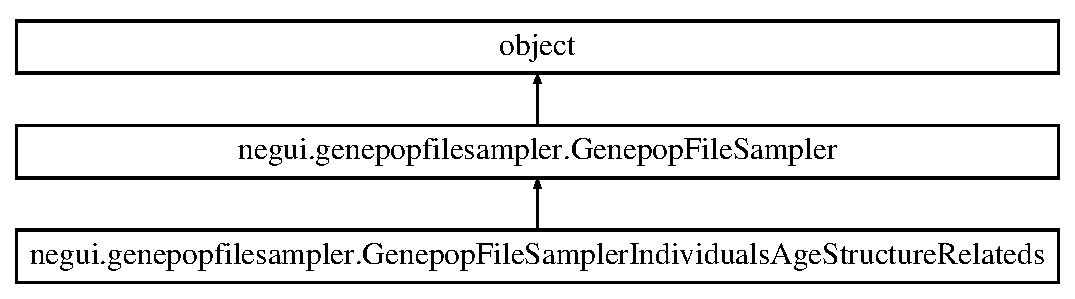
\includegraphics[height=3.000000cm]{classnegui_1_1genepopfilesampler_1_1GenepopFileSamplerIndividualsAgeStructureRelateds}
\end{center}
\end{figure}
\subsection*{Public Member Functions}
\begin{DoxyCompactItemize}
\item 
def {\bfseries \+\_\+\+\_\+init\+\_\+\+\_\+} (self, o\+\_\+genepopfilemanager, o\+\_\+genepopfilesampleparams)\hypertarget{classnegui_1_1genepopfilesampler_1_1GenepopFileSamplerIndividualsAgeStructureRelateds_aa74e2bb52923a31c31a6a2ca54bda6e0}{}\label{classnegui_1_1genepopfilesampler_1_1GenepopFileSamplerIndividualsAgeStructureRelateds_aa74e2bb52923a31c31a6a2ca54bda6e0}

\item 
def \hyperlink{classnegui_1_1genepopfilesampler_1_1GenepopFileSamplerIndividualsAgeStructureRelateds_a2c1d8215c48697cf7f81ba45c31435aa}{do\+Sample} (self)
\end{DoxyCompactItemize}


\subsection{Detailed Description}
\begin{DoxyVerb}This sampler class meant to implement Tiago's sampling code in his
sampleIndivsRelated.py module.  It samples pairs of individuals who
share parentage.  The GenepopFileSampleParams object used by instances
of this class has the values Tiagos module takes at the command line 
that restrict the fraction of indiv (per gen) who should be siblings,
as well as a total individuals per generation.  Note that his
startGen endGen paramters are already implemented via the Sampler's
li_population_numbers parameter.
\end{DoxyVerb}
 

Definition at line 1480 of file genepopfilesampler.\+py.



\subsection{Member Function Documentation}
\index{negui\+::genepopfilesampler\+::\+Genepop\+File\+Sampler\+Individuals\+Age\+Structure\+Relateds@{negui\+::genepopfilesampler\+::\+Genepop\+File\+Sampler\+Individuals\+Age\+Structure\+Relateds}!do\+Sample@{do\+Sample}}
\index{do\+Sample@{do\+Sample}!negui\+::genepopfilesampler\+::\+Genepop\+File\+Sampler\+Individuals\+Age\+Structure\+Relateds@{negui\+::genepopfilesampler\+::\+Genepop\+File\+Sampler\+Individuals\+Age\+Structure\+Relateds}}
\subsubsection[{\texorpdfstring{do\+Sample(self)}{doSample(self)}}]{\setlength{\rightskip}{0pt plus 5cm}def negui.\+genepopfilesampler.\+Genepop\+File\+Sampler\+Individuals\+Age\+Structure\+Relateds.\+do\+Sample (
\begin{DoxyParamCaption}
\item[{}]{self}
\end{DoxyParamCaption}
)}\hypertarget{classnegui_1_1genepopfilesampler_1_1GenepopFileSamplerIndividualsAgeStructureRelateds_a2c1d8215c48697cf7f81ba45c31435aa}{}\label{classnegui_1_1genepopfilesampler_1_1GenepopFileSamplerIndividualsAgeStructureRelateds_a2c1d8215c48697cf7f81ba45c31435aa}
\begin{DoxyVerb}Sample siblings in pairs/parentage until the percent sibs threshold
is reached, then pad with non-relateds.  See Tiagos code in his 
sampleIndivsRelated.py module.
\end{DoxyVerb}
 

Definition at line 1545 of file genepopfilesampler.\+py.


\begin{DoxyCode}
1545     \textcolor{keyword}{def }\hyperlink{classnegui_1_1genepopfilesampler_1_1GenepopFileSamplerIndividualsAgeStructureRelateds_a2c1d8215c48697cf7f81ba45c31435aa}{doSample}( self ):
1546         \textcolor{stringliteral}{'''}
1547 \textcolor{stringliteral}{        Sample siblings in pairs/parentage until the percent sibs threshold}
1548 \textcolor{stringliteral}{        is reached, then pad with non-relateds.  See Tiagos code in his }
1549 \textcolor{stringliteral}{        sampleIndivsRelated.py module.}
1550 \textcolor{stringliteral}{        '''}
1551         FIELD\_NAME\_AGE=\textcolor{stringliteral}{"age"}
1552         FIELD\_NAME\_MOTHER=\textcolor{stringliteral}{"mother"}
1553         FIELD\_NAME\_FATHER=\textcolor{stringliteral}{"father"}
1554 
1555         \textcolor{comment}{#estimator driver needs a pop number subsample when it adds calls to the NeEstimator:}
1556         self.filemanager.subsamplePopulationsByList( self.sampleparams.population\_numbers,
1557                                                     s\_subsample\_tag=
      self.sampleparams.population\_subsample\_name )
1558 
1559         dli\_indiv\_index\_lists\_by\_pop\_number=\{\}
1560         
1561         i\_replicate\_count=self.sampleparams.replicates
1562 
1563         \textcolor{keywordflow}{for} i\_replicate\_number \textcolor{keywordflow}{in} range(i\_replicate\_count ):
1564 
1565             \textcolor{keywordflow}{for} i\_pop\_number \textcolor{keywordflow}{in} self.sampleparams.population\_numbers:
1566 
1567                 ls\_id\_list=self.filemanager.getListIndividuals( i\_pop\_number )
1568                 \textcolor{stringliteral}{'''}
1569 \textcolor{stringliteral}{                We assume that the list of Id's in the individual list}
1570 \textcolor{stringliteral}{                is indexed such that the zeroth id corresponds to the first}
1571 \textcolor{stringliteral}{                indiv as ordered in the genepop file, the [1] indexed id}
1572 \textcolor{stringliteral}{                is the second indiv, etc.}
1573 \textcolor{stringliteral}{                '''}
1574                 i\_tot\_indiv=len( ls\_id\_list )
1575 
1576                 dli\_indiv\_index\_by\_parentage=\{\}
1577                 li\_all\_indivs\_this\_pop=[]
1578 
1579                 \textcolor{stringliteral}{'''}
1580 \textcolor{stringliteral}{                Note that in py3, you can divide 2 ints, at least}
1581 \textcolor{stringliteral}{                when one's a literal like "100", and get a float}
1582 \textcolor{stringliteral}{                but in py2 you get the floor of the ratio, i.e. zero}
1583 \textcolor{stringliteral}{                for any ratio < 1/1.  Note that Tiago's sampleIndivsRelated.py}
1584 \textcolor{stringliteral}{                code has the  "int( arg[2] )/100" formulation, so that}
1585 \textcolor{stringliteral}{                the code is no longer py2 compatible without his import statement:}
1586 \textcolor{stringliteral}{                from \_\_future\_\_ import division.}
1587 \textcolor{stringliteral}{}
1588 \textcolor{stringliteral}{                We try version-neutral syntax:}
1589 \textcolor{stringliteral}{                '''}
1590 
1591                 f\_fraction\_relateds=old\_div(self.sampleparams.percent\_relateds, 100.0)
1592 
1593                 \textcolor{keyword}{assert} type( f\_fraction\_relateds ) == float,  \(\backslash\)
1594                         \textcolor{stringliteral}{"In GenepopFileSamplerIndividualsAgeStructureRelateds Instance, "} \(\backslash\)
1595                                 + \textcolor{stringliteral}{"def doSample, non-float result of division."}
1596 
1597                 \textcolor{keywordflow}{for} idx \textcolor{keywordflow}{in} range( i\_tot\_indiv ):
1598 
1599                     s\_id=ls\_id\_list[ idx ]
1600                     o\_id\_vals=GenepopIndivIdVals( s\_id, 
1601                                         self.sampleparams.fields )
1602                     i\_age=o\_id\_vals.getVal( FIELD\_NAME\_AGE )
1603 
1604                     \textcolor{keywordflow}{if} i\_age > 1:
1605                         \textcolor{keywordflow}{continue}
1606                     \textcolor{comment}{#end if too old, continue}
1607 
1608                     i\_mother=o\_id\_vals.getVal( FIELD\_NAME\_MOTHER )
1609                     i\_father=o\_id\_vals.getVal( FIELD\_NAME\_FATHER )
1610 
1611                     ti\_parentage=( i\_mother, i\_father )
1612 
1613                     \textcolor{stringliteral}{'''}
1614 \textcolor{stringliteral}{                    Note that idx+1 gives the number of the individual as ordered by its}
1615 \textcolor{stringliteral}{                    entry in the "pop" section of this pop in the genepop file, as used}
1616 \textcolor{stringliteral}{                    by the genepopfilemanager object to point to it's byte address in }
1617 \textcolor{stringliteral}{                    the file.  Thus it's our way of collecting samples of individuals }
1618 \textcolor{stringliteral}{                    and passing them into the genepop file manager object's subsampling }
1619 \textcolor{stringliteral}{                    records (its attribute \_\_indiv\_subsamples).}
1620 \textcolor{stringliteral}{                    '''}
1621                     i\_indiv\_number=idx+1
1622                     li\_all\_indivs\_this\_pop.append( i\_indiv\_number )
1623                     dli\_indiv\_index\_by\_parentage.setdefault( \(\backslash\)
1624                                 ti\_parentage, [] ).append( i\_indiv\_number ) 
1625 
1626                 \textcolor{comment}{#end for each individual's id   }
1627                 
1628                 i\_tot\_indivs=len( li\_all\_indivs\_this\_pop )
1629 
1630                 i\_target\_total\_indivs=i\_tot\_indivs
1631 
1632                 \textcolor{comment}{#If too few indivs, error, else reduce the target total if over}
1633                 \textcolor{comment}{#the max, to the max}
1634                 \textcolor{keywordflow}{if} i\_target\_total\_indivs < self.sampleparams.min\_indiv\_per\_gen:
1635                     s\_msg=\textcolor{stringliteral}{"In GenepopFileSamplerIndividualsAgeStructureRelateds, "} \(\backslash\)
1636                             + \textcolor{stringliteral}{"instance, total individuals, "} \(\backslash\)
1637                             + str( i\_tot\_indivs ) \(\backslash\)
1638                             + \textcolor{stringliteral}{"is under the value given as minimum, "} \(\backslash\)
1639                             + str( self.sampleparams.min\_indiv\_per\_gen ) \(\backslash\)
1640                             + \textcolor{stringliteral}{"."}
1641                     \textcolor{keywordflow}{raise} Exception( s\_msg )
1642                 \textcolor{keywordflow}{elif} i\_target\_total\_indivs > self.sampleparams.max\_indiv\_per\_gen:
1643                     i\_target\_total\_indivs=self.sampleparams.max\_indiv\_per\_gen
1644                 \textcolor{comment}{#end if total individuals under min, error}
1645 
1646 
1647                 i\_target\_total\_relateds=i\_target\_total\_indivs * f\_fraction\_relateds
1648                 li\_relateds\_collected=self.\hyperlink{classnegui_1_1genepopfilesampler_1_1GenepopFileSamplerIndividualsAgeStructureRelateds_af76a2ae0e6f84e4fe8bc8e5856e3a16b}{\_\_get\_siblings}( dli\_indiv\_index\_by\_parentage, 
1649                                                                     i\_target\_total\_relateds )
1650             
1651                 \textcolor{keywordflow}{for} i\_related \textcolor{keywordflow}{in} li\_relateds\_collected:
1652                     li\_all\_indivs\_this\_pop.remove( i\_related )
1653                 \textcolor{comment}{#end for each related collected}
1654 
1655                 \textcolor{comment}{#rename for clarity}
1656                 li\_individuals\_with\_relateds\_removed=\(\backslash\)
1657                                     li\_all\_indivs\_this\_pop
1658 
1659                 i\_total\_relateds\_collected=len( li\_relateds\_collected )
1660 
1661                 i\_non\_relateds\_needed\_to\_make\_total= i\_target\_total\_indivs \(\backslash\)
1662                                                     - i\_total\_relateds\_collected
1663                 li\_non\_relateds\_collected = []
1664 
1665                 \textcolor{keywordflow}{if} i\_non\_relateds\_needed\_to\_make\_total > 0:
1666 
1667                     \textcolor{keywordflow}{try}:
1668                         li\_non\_relateds\_collected=random.sample( \(\backslash\)
1669                                             li\_individuals\_with\_relateds\_removed, 
1670                                                 i\_non\_relateds\_needed\_to\_make\_total )
1671                     \textcolor{keywordflow}{except} Exception \textcolor{keyword}{as} oex:
1672 
1673                         \textcolor{comment}{#We may be changing the algorithm to test}
1674                         \textcolor{comment}{#for the sample size vs the length of the list sampled}
1675                         \textcolor{comment}{#but for now we catch errors:}
1676                         s\_sample\_error\_msg= \(\backslash\)
1677                                 \textcolor{stringliteral}{"In GenepopFileSamplerIndividualsAgeStructureRelateds "} \(\backslash\)
1678                                 + \textcolor{stringliteral}{"instance, def doSample, "}  \(\backslash\)
1679                                 + \textcolor{stringliteral}{"random.sample failed on list of "} \(\backslash\)
1680                                 + str( len( li\_individuals\_with\_relateds\_removed ) ) \(\backslash\)
1681                                 + \textcolor{stringliteral}{" individuals.  Target total to be sampled: "} \(\backslash\)
1682                                 + str( i\_non\_relateds\_needed\_to\_make\_total ) + \textcolor{stringliteral}{"."}
1683 
1684                         s\_msg=s\_sample\_error\_msg + \textcolor{stringliteral}{"  Exception: "} + str( oex ) + \textcolor{stringliteral}{"."}
1685                         \textcolor{keywordflow}{raise} Exception( s\_msg )
1686                     \textcolor{comment}{#try . . . except . . . }
1687 
1688                 \textcolor{keywordflow}{elif} i\_non\_relateds\_needed\_to\_make\_total < 0:
1689                     \textcolor{stringliteral}{'''}
1690 \textcolor{stringliteral}{                    Not sure this case is possible, but suspect it may be}
1691 \textcolor{stringliteral}{                    due either to rounding, or the pairwise collecting of}
1692 \textcolor{stringliteral}{                    siblings.  We may after trials, decide to except an overage}
1693 \textcolor{stringliteral}{                    of one, but for now let's throw an error:}
1694 \textcolor{stringliteral}{                    '''}
1695 
1696                     s\_msg=\textcolor{stringliteral}{"In GenepopFileSamplerIndividualsAgeStructureRelateds "} \(\backslash\)
1697                                 + \textcolor{stringliteral}{"instance, def doSample, "}  \(\backslash\)
1698                                 + \textcolor{stringliteral}{"relateds collected, "} \(\backslash\)
1699                                 + str( i\_total\_relateds\_collected ) \(\backslash\)
1700                                 + \textcolor{stringliteral}{", exceeds the maximum set as valid, "} \(\backslash\)
1701                                 + str( self.sampleparams.max\_indiv\_per\_gen ) \(\backslash\)
1702                                 + \textcolor{stringliteral}{"."}
1703                     \textcolor{keywordflow}{raise} Exception
1704                 \textcolor{comment}{#end if need to collect at least one non\_relateds}
1705 
1706                 li\_indiv\_sample=li\_relateds\_collected + li\_non\_relateds\_collected
1707 
1708                 dli\_indiv\_index\_lists\_by\_pop\_number[ i\_pop\_number ] = li\_indiv\_sample
1709             \textcolor{comment}{#end for each pop number}
1710 
1711             s\_this\_subsample\_name=make\_subsample\_tag( \(\backslash\)
1712                                 self.sampleparams.sample\_param\_value, 
1713                                 i\_replicate\_number, 
1714                                 SCHEME\_RELATEDS,
1715                                 s\_prefix=self.sampleparams.sample\_tag\_base )
1716 
1717             self.filemanager.subsampleIndividualsByNumberList( \(\backslash\)
1718                                     dli\_indiv\_index\_lists\_by\_pop\_number, 
1719                                                     s\_this\_subsample\_name )
1720         \textcolor{comment}{#end for each replicate}
1721         \textcolor{keywordflow}{return}
\end{DoxyCode}


The documentation for this class was generated from the following file\+:\begin{DoxyCompactItemize}
\item 
genepopfilesampler.\+py\end{DoxyCompactItemize}

\hypertarget{classnegui_1_1genepopfilesampler_1_1GenepopFileSamplerIndividualsByCriteria}{}\section{negui.\+genepopfilesampler.\+Genepop\+File\+Sampler\+Individuals\+By\+Criteria Class Reference}
\label{classnegui_1_1genepopfilesampler_1_1GenepopFileSamplerIndividualsByCriteria}\index{negui.\+genepopfilesampler.\+Genepop\+File\+Sampler\+Individuals\+By\+Criteria@{negui.\+genepopfilesampler.\+Genepop\+File\+Sampler\+Individuals\+By\+Criteria}}
Inheritance diagram for negui.\+genepopfilesampler.\+Genepop\+File\+Sampler\+Individuals\+By\+Criteria\+:\begin{figure}[H]
\begin{center}
\leavevmode
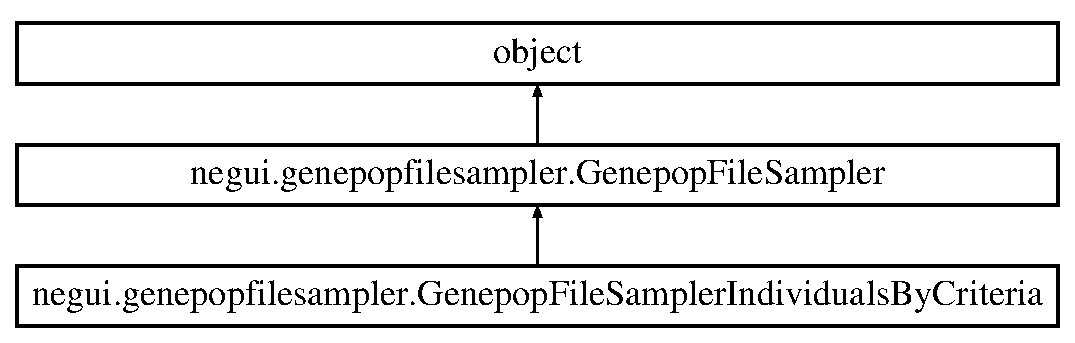
\includegraphics[height=3.000000cm]{classnegui_1_1genepopfilesampler_1_1GenepopFileSamplerIndividualsByCriteria}
\end{center}
\end{figure}
\subsection*{Public Member Functions}
\begin{DoxyCompactItemize}
\item 
def {\bfseries \+\_\+\+\_\+init\+\_\+\+\_\+} (self, o\+\_\+genepopfilemanager, o\+\_\+genepopfilesampleparams)\hypertarget{classnegui_1_1genepopfilesampler_1_1GenepopFileSamplerIndividualsByCriteria_a8e1ef3907b3d37dccf9174e66c210d0b}{}\label{classnegui_1_1genepopfilesampler_1_1GenepopFileSamplerIndividualsByCriteria_a8e1ef3907b3d37dccf9174e66c210d0b}

\item 
def {\bfseries do\+Sample} (self)\hypertarget{classnegui_1_1genepopfilesampler_1_1GenepopFileSamplerIndividualsByCriteria_aa40b9d843febb0279324744b898d9b3d}{}\label{classnegui_1_1genepopfilesampler_1_1GenepopFileSamplerIndividualsByCriteria_aa40b9d843febb0279324744b898d9b3d}

\end{DoxyCompactItemize}


\subsection{Detailed Description}
\begin{DoxyVerb}Samples by criteria applied to fields in individual ids.  
Instances of this class use the sample params class GenepopFileSampleParamsCriteria
To pass along to their GenepopFileManager instance attributes the criteria
for selecting individuals.
\end{DoxyVerb}
 

Definition at line 1994 of file genepopfilesampler.\+py.



The documentation for this class was generated from the following file\+:\begin{DoxyCompactItemize}
\item 
genepopfilesampler.\+py\end{DoxyCompactItemize}

\hypertarget{classnegui_1_1genepopfilesampler_1_1GenepopFileSamplerIndividualsByCriteriaFactored}{}\section{negui.\+genepopfilesampler.\+Genepop\+File\+Sampler\+Individuals\+By\+Criteria\+Factored Class Reference}
\label{classnegui_1_1genepopfilesampler_1_1GenepopFileSamplerIndividualsByCriteriaFactored}\index{negui.\+genepopfilesampler.\+Genepop\+File\+Sampler\+Individuals\+By\+Criteria\+Factored@{negui.\+genepopfilesampler.\+Genepop\+File\+Sampler\+Individuals\+By\+Criteria\+Factored}}
Inheritance diagram for negui.\+genepopfilesampler.\+Genepop\+File\+Sampler\+Individuals\+By\+Criteria\+Factored\+:\begin{figure}[H]
\begin{center}
\leavevmode
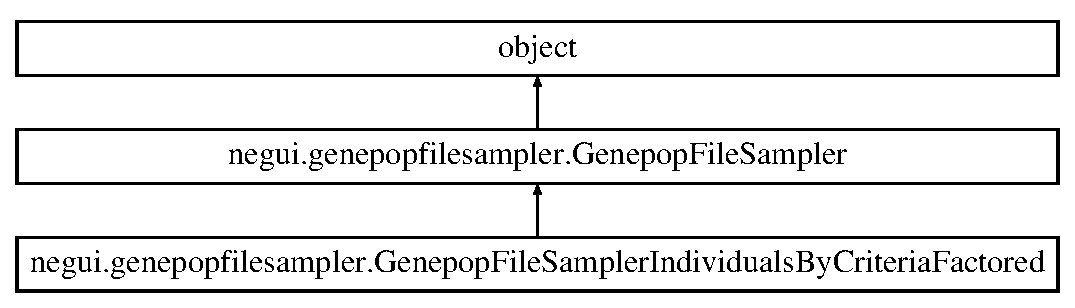
\includegraphics[height=3.000000cm]{classnegui_1_1genepopfilesampler_1_1GenepopFileSamplerIndividualsByCriteriaFactored}
\end{center}
\end{figure}
\subsection*{Public Member Functions}
\begin{DoxyCompactItemize}
\item 
def {\bfseries \+\_\+\+\_\+init\+\_\+\+\_\+} (self, o\+\_\+genepopfilemanager, o\+\_\+genepopfilesampleparams)\hypertarget{classnegui_1_1genepopfilesampler_1_1GenepopFileSamplerIndividualsByCriteriaFactored_a8c5aa4e8af5d35a2ab9983a8e64cec0e}{}\label{classnegui_1_1genepopfilesampler_1_1GenepopFileSamplerIndividualsByCriteriaFactored_a8c5aa4e8af5d35a2ab9983a8e64cec0e}

\item 
def {\bfseries do\+Sample} (self)\hypertarget{classnegui_1_1genepopfilesampler_1_1GenepopFileSamplerIndividualsByCriteriaFactored_afb4984d0dc7060e94765116320987b4d}{}\label{classnegui_1_1genepopfilesampler_1_1GenepopFileSamplerIndividualsByCriteriaFactored_afb4984d0dc7060e94765116320987b4d}

\end{DoxyCompactItemize}


\subsection{Detailed Description}
\begin{DoxyVerb}Motivation for class creation:  need a way to sample cohorts (indiv
of a pop with same age-value) for multiple ages for each pop in 
a genepop file, and then, for each cohort for a give pop, apply a maximum
pop size (i.e. a max cohort size).

To that end added to class GenepopFileSampleParamsCriteria a "__max_pop_size"
attribute, used by this class, which can sample as above by client providing
a GenepopFileSampleParamsCriteria object with one criteria for each cohort
(i.e. %age%==i, to get cohort for individuals with age i).  

To get s factored set such as the cohort descripted above, this class
is similar to GenepopFileSamplerIndividualsByCriteria, but
instead of selecting individuals that meet all the criteria (as provided
by the GenepopIndivCriterion instances wrapped in the GenepopIndivCriteria
object member of the GenepopFileSampleParamsCriteria object), each criterion
is first sampled and added to the GenepopFileManager attribute as a separate
subsample.  After all subsamples are created, then, for each population in
the population list (as given by the GenepopFileSampleParamsCriteria object)
they are combined (set.union) by the def in the GenepopFileManager 
combineIndividualSubsamples.
\end{DoxyVerb}
 

Definition at line 2035 of file genepopfilesampler.\+py.



The documentation for this class was generated from the following file\+:\begin{DoxyCompactItemize}
\item 
genepopfilesampler.\+py\end{DoxyCompactItemize}

\hypertarget{classnegui_1_1genepopfilesampler_1_1GenepopFileSamplerIndividualsByCriteriaGrouped}{}\section{negui.\+genepopfilesampler.\+Genepop\+File\+Sampler\+Individuals\+By\+Criteria\+Grouped Class Reference}
\label{classnegui_1_1genepopfilesampler_1_1GenepopFileSamplerIndividualsByCriteriaGrouped}\index{negui.\+genepopfilesampler.\+Genepop\+File\+Sampler\+Individuals\+By\+Criteria\+Grouped@{negui.\+genepopfilesampler.\+Genepop\+File\+Sampler\+Individuals\+By\+Criteria\+Grouped}}
Inheritance diagram for negui.\+genepopfilesampler.\+Genepop\+File\+Sampler\+Individuals\+By\+Criteria\+Grouped\+:\begin{figure}[H]
\begin{center}
\leavevmode
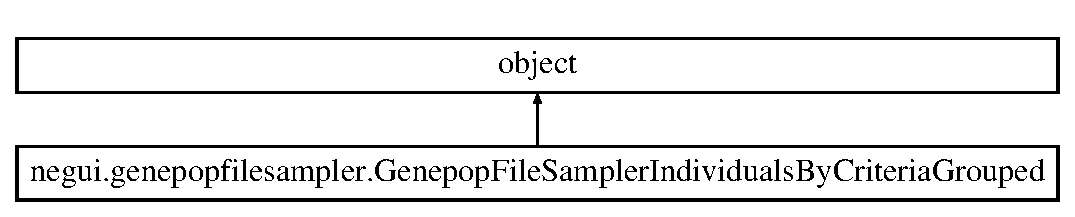
\includegraphics[height=2.000000cm]{classnegui_1_1genepopfilesampler_1_1GenepopFileSamplerIndividualsByCriteriaGrouped}
\end{center}
\end{figure}
\subsection*{Public Member Functions}
\begin{DoxyCompactItemize}
\item 
def {\bfseries \+\_\+\+\_\+init\+\_\+\+\_\+} (self, o\+\_\+genepopfilemanager, o\+\_\+genepopfilesampleparams)\hypertarget{classnegui_1_1genepopfilesampler_1_1GenepopFileSamplerIndividualsByCriteriaGrouped_a47bba07ea5592ffbda7ef58c78e194e2}{}\label{classnegui_1_1genepopfilesampler_1_1GenepopFileSamplerIndividualsByCriteriaGrouped_a47bba07ea5592ffbda7ef58c78e194e2}

\item 
def {\bfseries do\+Sample} (self)\hypertarget{classnegui_1_1genepopfilesampler_1_1GenepopFileSamplerIndividualsByCriteriaGrouped_a6bdd6f8fd7d56c41f14cf9744e862766}{}\label{classnegui_1_1genepopfilesampler_1_1GenepopFileSamplerIndividualsByCriteriaGrouped_a6bdd6f8fd7d56c41f14cf9744e862766}

\end{DoxyCompactItemize}


\subsection{Detailed Description}
\begin{DoxyVerb}Motivaing case:  Need a way to implement Tiago's sibling sampling
scheme.  As such, I need to group individuals in sim-generated
pops, from the AgeStructureNe code, by parentage (sibling groups,
defined, for two individuals,  as indiv_1.mother==indiv_2.mother, 
and same for father), operating only on individuals of age==1.  

I'm generalizing the case to be able to group indiviudals (in a given
pop inside a genepop file) by matching their field values, for one or
more fields.  Further, this sampling would then be followed by applying
a criteria to each individual.
\end{DoxyVerb}
 

Definition at line 2110 of file genepopfilesampler.\+py.



The documentation for this class was generated from the following file\+:\begin{DoxyCompactItemize}
\item 
genepopfilesampler.\+py\end{DoxyCompactItemize}

\hypertarget{classnegui_1_1genepopfilesampler_1_1GenepopFileSamplerIndividualsByProportion}{}\section{negui.\+genepopfilesampler.\+Genepop\+File\+Sampler\+Individuals\+By\+Proportion Class Reference}
\label{classnegui_1_1genepopfilesampler_1_1GenepopFileSamplerIndividualsByProportion}\index{negui.\+genepopfilesampler.\+Genepop\+File\+Sampler\+Individuals\+By\+Proportion@{negui.\+genepopfilesampler.\+Genepop\+File\+Sampler\+Individuals\+By\+Proportion}}
Inheritance diagram for negui.\+genepopfilesampler.\+Genepop\+File\+Sampler\+Individuals\+By\+Proportion\+:\begin{figure}[H]
\begin{center}
\leavevmode
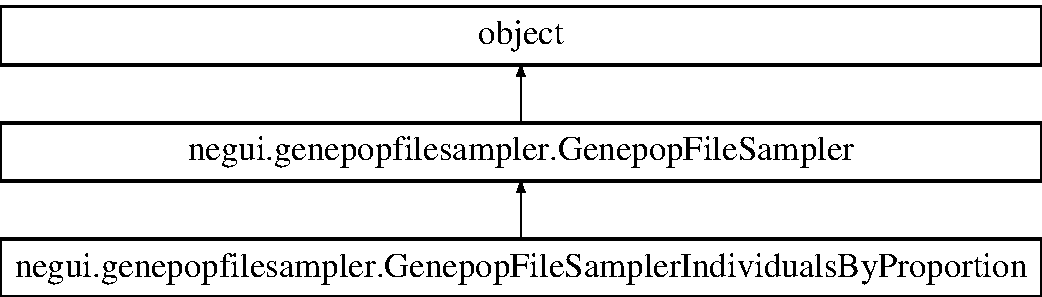
\includegraphics[height=3.000000cm]{classnegui_1_1genepopfilesampler_1_1GenepopFileSamplerIndividualsByProportion}
\end{center}
\end{figure}
\subsection*{Public Member Functions}
\begin{DoxyCompactItemize}
\item 
def {\bfseries \+\_\+\+\_\+init\+\_\+\+\_\+} (self, o\+\_\+genepopfilemanager, o\+\_\+genepopfilesampleparams)\hypertarget{classnegui_1_1genepopfilesampler_1_1GenepopFileSamplerIndividualsByProportion_a1bc0babcecf6bbca34259328cae53b97}{}\label{classnegui_1_1genepopfilesampler_1_1GenepopFileSamplerIndividualsByProportion_a1bc0babcecf6bbca34259328cae53b97}

\item 
def \hyperlink{classnegui_1_1genepopfilesampler_1_1GenepopFileSamplerIndividualsByProportion_ad8170ea6661afa7bff72d484372209e3}{do\+Sample} (self)
\end{DoxyCompactItemize}


\subsection{Detailed Description}
\begin{DoxyVerb}GenepopFileManager object that samples the individuals in each population
according one or more proportions (percentages).
\end{DoxyVerb}
 

Definition at line 1356 of file genepopfilesampler.\+py.



\subsection{Member Function Documentation}
\index{negui\+::genepopfilesampler\+::\+Genepop\+File\+Sampler\+Individuals\+By\+Proportion@{negui\+::genepopfilesampler\+::\+Genepop\+File\+Sampler\+Individuals\+By\+Proportion}!do\+Sample@{do\+Sample}}
\index{do\+Sample@{do\+Sample}!negui\+::genepopfilesampler\+::\+Genepop\+File\+Sampler\+Individuals\+By\+Proportion@{negui\+::genepopfilesampler\+::\+Genepop\+File\+Sampler\+Individuals\+By\+Proportion}}
\subsubsection[{\texorpdfstring{do\+Sample(self)}{doSample(self)}}]{\setlength{\rightskip}{0pt plus 5cm}def negui.\+genepopfilesampler.\+Genepop\+File\+Sampler\+Individuals\+By\+Proportion.\+do\+Sample (
\begin{DoxyParamCaption}
\item[{}]{self}
\end{DoxyParamCaption}
)}\hypertarget{classnegui_1_1genepopfilesampler_1_1GenepopFileSamplerIndividualsByProportion_ad8170ea6661afa7bff72d484372209e3}{}\label{classnegui_1_1genepopfilesampler_1_1GenepopFileSamplerIndividualsByProportion_ad8170ea6661afa7bff72d484372209e3}
\begin{DoxyVerb}as of Mon Jul 11 20:17:02 MDT 2016, for simplicity, the GenepopFileManager subsampling
defs that subsample individuals or loci, do so across all populations,
so that the subset of populations given by this objects member sampleparams property 
"population_numbers", will only be applied as a filter when writeGenePopFile (or printGenePopFile)
is applied to this objects GenepopFileManager object (self.filemanager ). The call
to the GenepopFileManager.writeGenePopFile, will need to include among its args the 
population subsample name ( assigned as the GenepopFileSampleParams object's
member "population_subsample_name") 
\end{DoxyVerb}
 

Definition at line 1366 of file genepopfilesampler.\+py.


\begin{DoxyCode}
1366     \textcolor{keyword}{def }\hyperlink{classnegui_1_1genepopfilesampler_1_1GenepopFileSamplerIndividualsByProportion_ad8170ea6661afa7bff72d484372209e3}{doSample}( self ):
1367         \textcolor{stringliteral}{'''}
1368 \textcolor{stringliteral}{        as of Mon Jul 11 20:17:02 MDT 2016, for simplicity, the GenepopFileManager subsampling}
1369 \textcolor{stringliteral}{        defs that subsample individuals or loci, do so across all populations,}
1370 \textcolor{stringliteral}{        so that the subset of populations given by this objects member sampleparams property }
1371 \textcolor{stringliteral}{        "population\_numbers", will only be applied as a filter when writeGenePopFile (or printGenePopFile)}
1372 \textcolor{stringliteral}{        is applied to this objects GenepopFileManager object (self.filemanager ). The call}
1373 \textcolor{stringliteral}{        to the GenepopFileManager.writeGenePopFile, will need to include among its args the }
1374 \textcolor{stringliteral}{        population subsample name ( assigned as the GenepopFileSampleParams object's}
1375 \textcolor{stringliteral}{        member "population\_subsample\_name") }
1376 \textcolor{stringliteral}{        '''}
1377 
1378         self.filemanager.subsamplePopulationsByList( self.sampleparams.population\_numbers, 
1379                 s\_subsample\_tag=self.sampleparams.population\_subsample\_name )
1380 
1381         lf\_proportions=self.sampleparams.proportions
1382         i\_total\_replicates=self.sampleparams.replicates
1383 
1384         \textcolor{keywordflow}{for} f\_proportion \textcolor{keywordflow}{in} lf\_proportions:
1385             \textcolor{keywordflow}{for} i\_replicate\_number \textcolor{keywordflow}{in} range( i\_total\_replicates ):
1386 
1387                 s\_subsampletag=\textcolor{keywordtype}{None}
1388 
1389                 \textcolor{keywordflow}{if} self.sampleparams.sample\_tag \textcolor{keywordflow}{is} \textcolor{keywordflow}{not} \textcolor{keywordtype}{None}:
1390                     s\_subsampletag=self.sampleparams.sample\_tag
1391                 \textcolor{keywordflow}{else}:
1392                     \textcolor{comment}{#standardized subsample tag uses the proportion and the rep number:}
1393                     \textcolor{comment}{#note that the "." char delimiter will need to be replaced by a diff}
1394                     \textcolor{comment}{#char when using this tag to name input or output file names for}
1395                     \textcolor{comment}{#NeEstimator (which truncates filenames using pattern .* for some of }
1396                     \textcolor{comment}{#its output files)}
1397                     s\_subsampletag=make\_subsample\_tag(  f\_proportion, i\_replicate\_number , 
      SCHEME\_PROPORTION )
1398                 \textcolor{comment}{#end if tag exists use it else make one}
1399 
1400                 self.filemanager.subsampleIndividualsRandomlyByProportion( f\_proportion, s\_subsampletag ) 
1401             \textcolor{comment}{#end for each replicate number  }
1402         \textcolor{comment}{#end for each proportion}
1403         \textcolor{keywordflow}{return}
1404 \textcolor{comment}{#end class GenepopFileSamplerIndividualsByProportion}
1405 
\end{DoxyCode}


The documentation for this class was generated from the following file\+:\begin{DoxyCompactItemize}
\item 
genepopfilesampler.\+py\end{DoxyCompactItemize}

\hypertarget{classnegui_1_1genepopfilesampler_1_1GenepopFileSamplerIndividualsByRemoval}{}\section{negui.\+genepopfilesampler.\+Genepop\+File\+Sampler\+Individuals\+By\+Removal Class Reference}
\label{classnegui_1_1genepopfilesampler_1_1GenepopFileSamplerIndividualsByRemoval}\index{negui.\+genepopfilesampler.\+Genepop\+File\+Sampler\+Individuals\+By\+Removal@{negui.\+genepopfilesampler.\+Genepop\+File\+Sampler\+Individuals\+By\+Removal}}
Inheritance diagram for negui.\+genepopfilesampler.\+Genepop\+File\+Sampler\+Individuals\+By\+Removal\+:\begin{figure}[H]
\begin{center}
\leavevmode
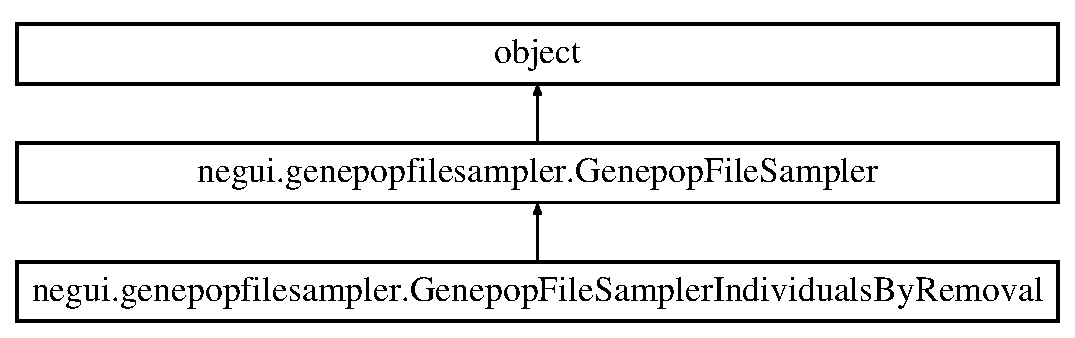
\includegraphics[height=3.000000cm]{classnegui_1_1genepopfilesampler_1_1GenepopFileSamplerIndividualsByRemoval}
\end{center}
\end{figure}
\subsection*{Public Member Functions}
\begin{DoxyCompactItemize}
\item 
def {\bfseries \+\_\+\+\_\+init\+\_\+\+\_\+} (self, o\+\_\+genepopfilemanager, o\+\_\+genepopfilesampleparams)\hypertarget{classnegui_1_1genepopfilesampler_1_1GenepopFileSamplerIndividualsByRemoval_aeba1258d811dd266cb3378212a4a1926}{}\label{classnegui_1_1genepopfilesampler_1_1GenepopFileSamplerIndividualsByRemoval_aeba1258d811dd266cb3378212a4a1926}

\item 
def {\bfseries do\+Sample} (self)\hypertarget{classnegui_1_1genepopfilesampler_1_1GenepopFileSamplerIndividualsByRemoval_a89dd3d276b9f089ac4c46dd844e7a848}{}\label{classnegui_1_1genepopfilesampler_1_1GenepopFileSamplerIndividualsByRemoval_a89dd3d276b9f089ac4c46dd844e7a848}

\end{DoxyCompactItemize}


\subsection{Detailed Description}
\begin{DoxyVerb}GenepopFileSampler object that samples individuals in each population
according to an N-removal scheme, that is, by removing N individuals 
randomly from the population, some M number of times, for some list of Ns
\end{DoxyVerb}
 

Definition at line 1406 of file genepopfilesampler.\+py.



The documentation for this class was generated from the following file\+:\begin{DoxyCompactItemize}
\item 
genepopfilesampler.\+py\end{DoxyCompactItemize}

\hypertarget{classnegui_1_1genepopfilesampler_1_1GenepopFileSamplerLociByRangeAndPercentage}{}\section{negui.\+genepopfilesampler.\+Genepop\+File\+Sampler\+Loci\+By\+Range\+And\+Percentage Class Reference}
\label{classnegui_1_1genepopfilesampler_1_1GenepopFileSamplerLociByRangeAndPercentage}\index{negui.\+genepopfilesampler.\+Genepop\+File\+Sampler\+Loci\+By\+Range\+And\+Percentage@{negui.\+genepopfilesampler.\+Genepop\+File\+Sampler\+Loci\+By\+Range\+And\+Percentage}}
Inheritance diagram for negui.\+genepopfilesampler.\+Genepop\+File\+Sampler\+Loci\+By\+Range\+And\+Percentage\+:\begin{figure}[H]
\begin{center}
\leavevmode
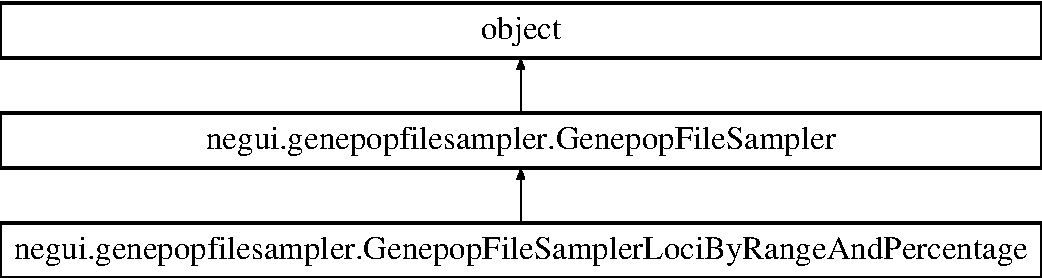
\includegraphics[height=3.000000cm]{classnegui_1_1genepopfilesampler_1_1GenepopFileSamplerLociByRangeAndPercentage}
\end{center}
\end{figure}
\subsection*{Public Member Functions}
\begin{DoxyCompactItemize}
\item 
def {\bfseries \+\_\+\+\_\+init\+\_\+\+\_\+} (self, o\+\_\+genepopfilemanager, o\+\_\+genepopfilesampleparams)\hypertarget{classnegui_1_1genepopfilesampler_1_1GenepopFileSamplerLociByRangeAndPercentage_a54d1db74e827c7d4ec18877699ea1ac3}{}\label{classnegui_1_1genepopfilesampler_1_1GenepopFileSamplerLociByRangeAndPercentage_a54d1db74e827c7d4ec18877699ea1ac3}

\item 
def {\bfseries do\+Sample} (self)\hypertarget{classnegui_1_1genepopfilesampler_1_1GenepopFileSamplerLociByRangeAndPercentage_a7ca84c7c483acade24446fef9d018686}{}\label{classnegui_1_1genepopfilesampler_1_1GenepopFileSamplerLociByRangeAndPercentage_a7ca84c7c483acade24446fef9d018686}

\end{DoxyCompactItemize}


\subsection{Detailed Description}
\begin{DoxyVerb}Sample loci from the ith to the jth, as listed in the 
genepop file individual entries.  Then, randomly select a subsample
by proportion, as given by the sample params "proportion" argument.
\end{DoxyVerb}
 

Definition at line 1759 of file genepopfilesampler.\+py.



The documentation for this class was generated from the following file\+:\begin{DoxyCompactItemize}
\item 
genepopfilesampler.\+py\end{DoxyCompactItemize}

\hypertarget{classnegui_1_1genepopfilesampler_1_1GenepopFileSamplerLociByRangeAndSampleTotalList}{}\section{negui.\+genepopfilesampler.\+Genepop\+File\+Sampler\+Loci\+By\+Range\+And\+Sample\+Total\+List Class Reference}
\label{classnegui_1_1genepopfilesampler_1_1GenepopFileSamplerLociByRangeAndSampleTotalList}\index{negui.\+genepopfilesampler.\+Genepop\+File\+Sampler\+Loci\+By\+Range\+And\+Sample\+Total\+List@{negui.\+genepopfilesampler.\+Genepop\+File\+Sampler\+Loci\+By\+Range\+And\+Sample\+Total\+List}}
Inheritance diagram for negui.\+genepopfilesampler.\+Genepop\+File\+Sampler\+Loci\+By\+Range\+And\+Sample\+Total\+List\+:\begin{figure}[H]
\begin{center}
\leavevmode
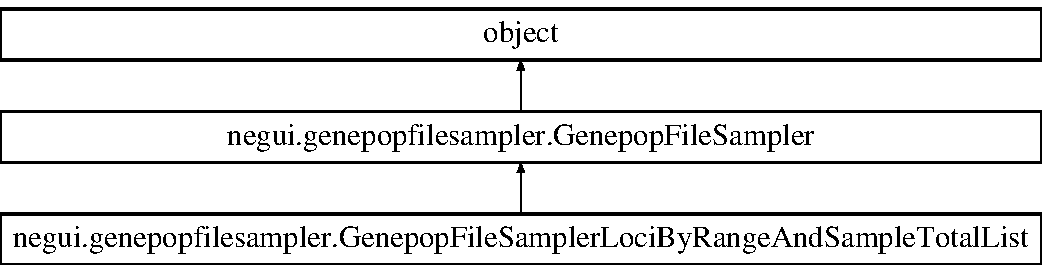
\includegraphics[height=3.000000cm]{classnegui_1_1genepopfilesampler_1_1GenepopFileSamplerLociByRangeAndSampleTotalList}
\end{center}
\end{figure}
\subsection*{Public Member Functions}
\begin{DoxyCompactItemize}
\item 
def {\bfseries \+\_\+\+\_\+init\+\_\+\+\_\+} (self, o\+\_\+genepopfilemanager, o\+\_\+genepopfilesampleparams)\hypertarget{classnegui_1_1genepopfilesampler_1_1GenepopFileSamplerLociByRangeAndSampleTotalList_a67bb332cbf92b3f3f07f15905b2e40d5}{}\label{classnegui_1_1genepopfilesampler_1_1GenepopFileSamplerLociByRangeAndSampleTotalList_a67bb332cbf92b3f3f07f15905b2e40d5}

\item 
def {\bfseries do\+Sample} (self)\hypertarget{classnegui_1_1genepopfilesampler_1_1GenepopFileSamplerLociByRangeAndSampleTotalList_a4760540c2cbe3536e2f85772b1fd8dad}{}\label{classnegui_1_1genepopfilesampler_1_1GenepopFileSamplerLociByRangeAndSampleTotalList_a4760540c2cbe3536e2f85772b1fd8dad}

\end{DoxyCompactItemize}


\subsection{Detailed Description}
\begin{DoxyVerb}Sample loci from the ith to the jth, as listed in the 
genepop file individual entries. Sample N loci for each value
N in the paramater sample_totals list.
\end{DoxyVerb}
 

Definition at line 1793 of file genepopfilesampler.\+py.



The documentation for this class was generated from the following file\+:\begin{DoxyCompactItemize}
\item 
genepopfilesampler.\+py\end{DoxyCompactItemize}

\hypertarget{classnegui_1_1genepopfilesampler_1_1GenepopFileSamplerLociByRangeAndTotal}{}\section{negui.\+genepopfilesampler.\+Genepop\+File\+Sampler\+Loci\+By\+Range\+And\+Total Class Reference}
\label{classnegui_1_1genepopfilesampler_1_1GenepopFileSamplerLociByRangeAndTotal}\index{negui.\+genepopfilesampler.\+Genepop\+File\+Sampler\+Loci\+By\+Range\+And\+Total@{negui.\+genepopfilesampler.\+Genepop\+File\+Sampler\+Loci\+By\+Range\+And\+Total}}
Inheritance diagram for negui.\+genepopfilesampler.\+Genepop\+File\+Sampler\+Loci\+By\+Range\+And\+Total\+:\begin{figure}[H]
\begin{center}
\leavevmode
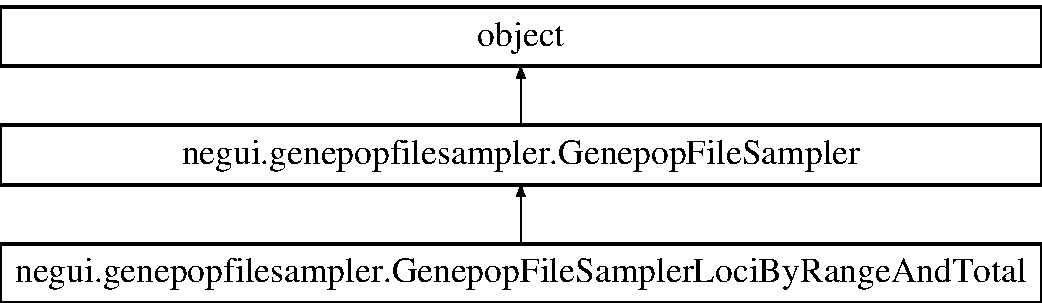
\includegraphics[height=3.000000cm]{classnegui_1_1genepopfilesampler_1_1GenepopFileSamplerLociByRangeAndTotal}
\end{center}
\end{figure}
\subsection*{Public Member Functions}
\begin{DoxyCompactItemize}
\item 
def {\bfseries \+\_\+\+\_\+init\+\_\+\+\_\+} (self, o\+\_\+genepopfilemanager, o\+\_\+genepopfilesampleparams)\hypertarget{classnegui_1_1genepopfilesampler_1_1GenepopFileSamplerLociByRangeAndTotal_ae2cef3a5eb0c188c3a2e147e8e93c79f}{}\label{classnegui_1_1genepopfilesampler_1_1GenepopFileSamplerLociByRangeAndTotal_ae2cef3a5eb0c188c3a2e147e8e93c79f}

\item 
def {\bfseries do\+Sample} (self)\hypertarget{classnegui_1_1genepopfilesampler_1_1GenepopFileSamplerLociByRangeAndTotal_a9295dd78f7b537acbefd16868cbcb58e}{}\label{classnegui_1_1genepopfilesampler_1_1GenepopFileSamplerLociByRangeAndTotal_a9295dd78f7b537acbefd16868cbcb58e}

\end{DoxyCompactItemize}


\subsection{Detailed Description}
\begin{DoxyVerb}Sample loci from the ith to the jth, as listed in the 
genepop file individual entries, and, if the max_total_loci 
is given, trunctate the total loci to this number by random sampling.
\end{DoxyVerb}
 

Definition at line 1725 of file genepopfilesampler.\+py.



The documentation for this class was generated from the following file\+:\begin{DoxyCompactItemize}
\item 
genepopfilesampler.\+py\end{DoxyCompactItemize}

\hypertarget{classnegui_1_1genepopfilesampler_1_1GenepopFileSamplerNone}{}\section{negui.\+genepopfilesampler.\+Genepop\+File\+Sampler\+None Class Reference}
\label{classnegui_1_1genepopfilesampler_1_1GenepopFileSamplerNone}\index{negui.\+genepopfilesampler.\+Genepop\+File\+Sampler\+None@{negui.\+genepopfilesampler.\+Genepop\+File\+Sampler\+None}}
Inheritance diagram for negui.\+genepopfilesampler.\+Genepop\+File\+Sampler\+None\+:\begin{figure}[H]
\begin{center}
\leavevmode
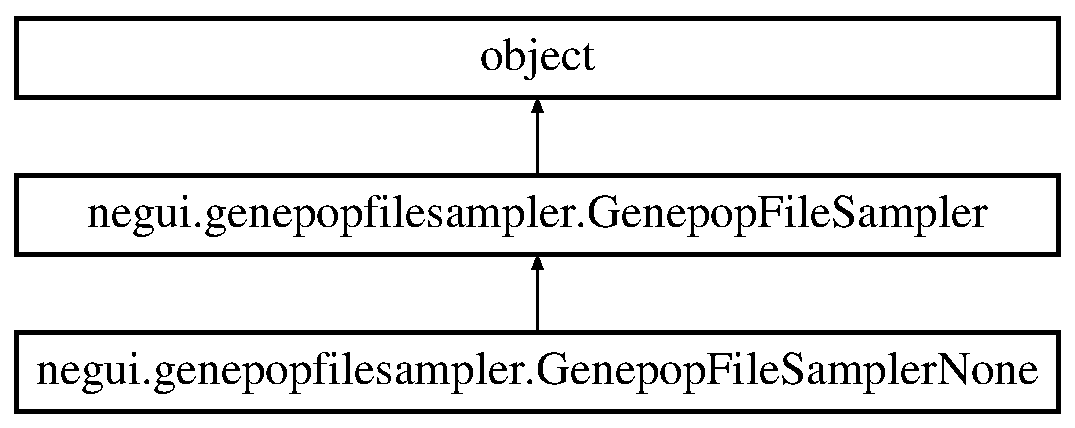
\includegraphics[height=3.000000cm]{classnegui_1_1genepopfilesampler_1_1GenepopFileSamplerNone}
\end{center}
\end{figure}
\subsection*{Public Member Functions}
\begin{DoxyCompactItemize}
\item 
def {\bfseries \+\_\+\+\_\+init\+\_\+\+\_\+} (self, o\+\_\+genepopfilemanager, o\+\_\+genepopfilesampleparams)\hypertarget{classnegui_1_1genepopfilesampler_1_1GenepopFileSamplerNone_a80379ccae205d2dc712898f429f81019}{}\label{classnegui_1_1genepopfilesampler_1_1GenepopFileSamplerNone_a80379ccae205d2dc712898f429f81019}

\item 
def \hyperlink{classnegui_1_1genepopfilesampler_1_1GenepopFileSamplerNone_a9e2c8b2d724ae8df46f21527486b485d}{do\+Sample} (self)
\end{DoxyCompactItemize}


\subsection{Detailed Description}
\begin{DoxyVerb}Does no sampling, except to apply a min and max pop size.  If
the population size exceeds the max, the max number is randomly
selected from among the individuals.
\end{DoxyVerb}
 

Definition at line 1833 of file genepopfilesampler.\+py.



\subsection{Member Function Documentation}
\index{negui\+::genepopfilesampler\+::\+Genepop\+File\+Sampler\+None@{negui\+::genepopfilesampler\+::\+Genepop\+File\+Sampler\+None}!do\+Sample@{do\+Sample}}
\index{do\+Sample@{do\+Sample}!negui\+::genepopfilesampler\+::\+Genepop\+File\+Sampler\+None@{negui\+::genepopfilesampler\+::\+Genepop\+File\+Sampler\+None}}
\subsubsection[{\texorpdfstring{do\+Sample(self)}{doSample(self)}}]{\setlength{\rightskip}{0pt plus 5cm}def negui.\+genepopfilesampler.\+Genepop\+File\+Sampler\+None.\+do\+Sample (
\begin{DoxyParamCaption}
\item[{}]{self}
\end{DoxyParamCaption}
)}\hypertarget{classnegui_1_1genepopfilesampler_1_1GenepopFileSamplerNone_a9e2c8b2d724ae8df46f21527486b485d}{}\label{classnegui_1_1genepopfilesampler_1_1GenepopFileSamplerNone_a9e2c8b2d724ae8df46f21527486b485d}
\begin{DoxyVerb}Simply add a subsample set that mimics the original
genepop pos, unless the pop indiv count is under min,
in which case reduce the sample to zero, or the orignal
exceeds the max, in which case randomly select the max
number of individuals.
\end{DoxyVerb}
 

Definition at line 1844 of file genepopfilesampler.\+py.


\begin{DoxyCode}
1844     \textcolor{keyword}{def }\hyperlink{classnegui_1_1genepopfilesampler_1_1GenepopFileSamplerNone_a9e2c8b2d724ae8df46f21527486b485d}{doSample}( self ):
1845         \textcolor{stringliteral}{'''}
1846 \textcolor{stringliteral}{        Simply add a subsample set that mimics the original}
1847 \textcolor{stringliteral}{        genepop pos, unless the pop indiv count is under min,}
1848 \textcolor{stringliteral}{        in which case reduce the sample to zero, or the orignal}
1849 \textcolor{stringliteral}{        exceeds the max, in which case randomly select the max}
1850 \textcolor{stringliteral}{        number of individuals.}
1851 \textcolor{stringliteral}{        '''}
1852         
1853         self.filemanager.subsamplePopulationsByList( self.sampleparams.population\_numbers,
1854                                         s\_subsample\_tag=self.sampleparams.population\_subsample\_name )
1855         \textcolor{stringliteral}{'''}
1856 \textcolor{stringliteral}{        Despite the fact that replicates will be indentical, we}
1857 \textcolor{stringliteral}{        still perform multi replicates if the replicates>1,}
1858 \textcolor{stringliteral}{        to keep form with other sampler schemes.}
1859 \textcolor{stringliteral}{        '''}
1860         \textcolor{keywordflow}{for} i\_replicate\_number \textcolor{keywordflow}{in} range( self.sampleparams.replicates ): 
1861 
1862             s\_this\_subsample\_name=make\_subsample\_tag( \(\backslash\)
1863                         self.sampleparams.sample\_param\_value, 
1864                         i\_replicate\_number, 
1865                         SCHEME\_NONE,
1866                         s\_prefix=self.sampleparams.sample\_tag\_base )
1867 
1868             self.filemanager.subsampleIndividualsByPopSize( self.sampleparams.min\_pop\_size,
1869                                                             self.sampleparams.max\_pop\_size,
1870                                                             s\_this\_subsample\_name )
1871         \textcolor{comment}{#end for each replicate}
1872 
1873         \textcolor{keywordflow}{return}
\end{DoxyCode}


The documentation for this class was generated from the following file\+:\begin{DoxyCompactItemize}
\item 
genepopfilesampler.\+py\end{DoxyCompactItemize}

\hypertarget{classnegui_1_1genepopindividualid_1_1GenepopIndivCriteria}{}\section{negui.\+genepopindividualid.\+Genepop\+Indiv\+Criteria Class Reference}
\label{classnegui_1_1genepopindividualid_1_1GenepopIndivCriteria}\index{negui.\+genepopindividualid.\+Genepop\+Indiv\+Criteria@{negui.\+genepopindividualid.\+Genepop\+Indiv\+Criteria}}
Inheritance diagram for negui.\+genepopindividualid.\+Genepop\+Indiv\+Criteria\+:\begin{figure}[H]
\begin{center}
\leavevmode
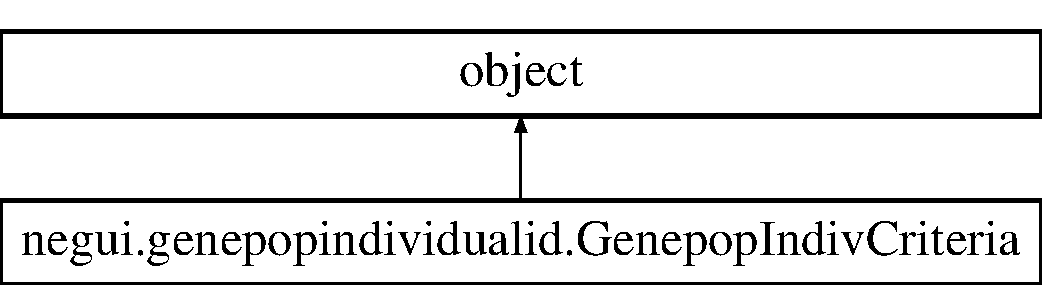
\includegraphics[height=2.000000cm]{classnegui_1_1genepopindividualid_1_1GenepopIndivCriteria}
\end{center}
\end{figure}
\subsection*{Public Member Functions}
\begin{DoxyCompactItemize}
\item 
def {\bfseries \+\_\+\+\_\+init\+\_\+\+\_\+} (self, lo\+\_\+criteria=None)\hypertarget{classnegui_1_1genepopindividualid_1_1GenepopIndivCriteria_af2dee1c4395c3be5eb236bb838d79b48}{}\label{classnegui_1_1genepopindividualid_1_1GenepopIndivCriteria_af2dee1c4395c3be5eb236bb838d79b48}

\item 
def \hyperlink{classnegui_1_1genepopindividualid_1_1GenepopIndivCriteria_a8b5b08b5100a7aaa759c26489b87eb34}{all\+Tests\+Are\+True} (self, ls\+\_\+field\+\_\+names, lv\+\_\+field\+\_\+values)
\item 
def \hyperlink{classnegui_1_1genepopindividualid_1_1GenepopIndivCriteria_a30cfe91fa9b4cb481ecf5cab3332ac56}{get\+Subset\+Of\+Criteria\+As\+New\+Criteria\+Object} (self, li\+\_\+criterion\+\_\+indices)
\item 
def {\bfseries copy} (self)\hypertarget{classnegui_1_1genepopindividualid_1_1GenepopIndivCriteria_adb2e780d64d41939ea2918cca0434457}{}\label{classnegui_1_1genepopindividualid_1_1GenepopIndivCriteria_adb2e780d64d41939ea2918cca0434457}

\item 
def {\bfseries add\+Criterion} (self, s\+\_\+criterion\+\_\+name, ls\+\_\+field\+\_\+names, s\+\_\+test)\hypertarget{classnegui_1_1genepopindividualid_1_1GenepopIndivCriteria_a871c920cf188bf93e6b3a30e26afb1a2}{}\label{classnegui_1_1genepopindividualid_1_1GenepopIndivCriteria_a871c920cf188bf93e6b3a30e26afb1a2}

\item 
def {\bfseries criteriacount} (self)\hypertarget{classnegui_1_1genepopindividualid_1_1GenepopIndivCriteria_a20f68e2cf59a14286d038fae4c3547df}{}\label{classnegui_1_1genepopindividualid_1_1GenepopIndivCriteria_a20f68e2cf59a14286d038fae4c3547df}

\item 
def {\bfseries criteria} (self)\hypertarget{classnegui_1_1genepopindividualid_1_1GenepopIndivCriteria_af0b41598685d0acf1607b2d1a80d46c7}{}\label{classnegui_1_1genepopindividualid_1_1GenepopIndivCriteria_af0b41598685d0acf1607b2d1a80d46c7}

\end{DoxyCompactItemize}


\subsection{Detailed Description}
\begin{DoxyVerb}Wraps a list of GenepopIndivCriteria.
Can evaluate all tests when a list of
field names and values is provided.
\end{DoxyVerb}
 

Definition at line 419 of file genepopindividualid.\+py.



\subsection{Member Function Documentation}
\index{negui\+::genepopindividualid\+::\+Genepop\+Indiv\+Criteria@{negui\+::genepopindividualid\+::\+Genepop\+Indiv\+Criteria}!all\+Tests\+Are\+True@{all\+Tests\+Are\+True}}
\index{all\+Tests\+Are\+True@{all\+Tests\+Are\+True}!negui\+::genepopindividualid\+::\+Genepop\+Indiv\+Criteria@{negui\+::genepopindividualid\+::\+Genepop\+Indiv\+Criteria}}
\subsubsection[{\texorpdfstring{all\+Tests\+Are\+True(self, ls\+\_\+field\+\_\+names, lv\+\_\+field\+\_\+values)}{allTestsAreTrue(self, ls_field_names, lv_field_values)}}]{\setlength{\rightskip}{0pt plus 5cm}def negui.\+genepopindividualid.\+Genepop\+Indiv\+Criteria.\+all\+Tests\+Are\+True (
\begin{DoxyParamCaption}
\item[{}]{self, }
\item[{}]{ls\+\_\+field\+\_\+names, }
\item[{}]{lv\+\_\+field\+\_\+values}
\end{DoxyParamCaption}
)}\hypertarget{classnegui_1_1genepopindividualid_1_1GenepopIndivCriteria_a8b5b08b5100a7aaa759c26489b87eb34}{}\label{classnegui_1_1genepopindividualid_1_1GenepopIndivCriteria_a8b5b08b5100a7aaa759c26489b87eb34}
\begin{DoxyVerb}Assumes field value list arg is in order such
that its nth value is corresponds to the nth
value in the list of field names.
\end{DoxyVerb}
 

Definition at line 467 of file genepopindividualid.\+py.


\begin{DoxyCode}
467     \textcolor{keyword}{def }\hyperlink{classnegui_1_1genepopindividualid_1_1GenepopIndivCriteria_a8b5b08b5100a7aaa759c26489b87eb34}{allTestsAreTrue}( self, ls\_field\_names, lv\_field\_values ):
468         \textcolor{stringliteral}{'''}
469 \textcolor{stringliteral}{        Assumes field value list arg is in order such}
470 \textcolor{stringliteral}{        that its nth value is corresponds to the nth}
471 \textcolor{stringliteral}{        value in the list of field names.}
472 \textcolor{stringliteral}{        '''}
473         db\_test\_results=self.\hyperlink{classnegui_1_1genepopindividualid_1_1GenepopIndivCriteria_a1bce8a4201a0935fe6d6ff03f06071ed}{\_\_get\_dict\_list\_test\_results}( ls\_field\_names, 
      lv\_field\_values )
474 
475 
476         \textcolor{stringliteral}{'''}
477 \textcolor{stringliteral}{        If the client called this def on an instance}
478 \textcolor{stringliteral}{        with no criteria to test, raise an exception:}
479 \textcolor{stringliteral}{        '''}
480         \textcolor{keywordflow}{if} len( db\_test\_results ) == 0:
481             s\_msg=\textcolor{stringliteral}{"In GenepopIndivCriteria instance, "} \(\backslash\)
482                     + \textcolor{stringliteral}{"def allTestsAreTrue, "} \(\backslash\)
483                     + \textcolor{stringliteral}{"called on an instance with no "} \(\backslash\)
484                     + \textcolor{stringliteral}{"criterion objects for tests."}
485             \textcolor{keywordflow}{raise} Exception( s\_msg )
486         \textcolor{comment}{#end if no test results}
487 
488         set\_test\_results=set( db\_test\_results.values() )
489         \textcolor{keywordflow}{return} set\_test\_results==\{\textcolor{keyword}{True}\}
490 
\end{DoxyCode}
\index{negui\+::genepopindividualid\+::\+Genepop\+Indiv\+Criteria@{negui\+::genepopindividualid\+::\+Genepop\+Indiv\+Criteria}!get\+Subset\+Of\+Criteria\+As\+New\+Criteria\+Object@{get\+Subset\+Of\+Criteria\+As\+New\+Criteria\+Object}}
\index{get\+Subset\+Of\+Criteria\+As\+New\+Criteria\+Object@{get\+Subset\+Of\+Criteria\+As\+New\+Criteria\+Object}!negui\+::genepopindividualid\+::\+Genepop\+Indiv\+Criteria@{negui\+::genepopindividualid\+::\+Genepop\+Indiv\+Criteria}}
\subsubsection[{\texorpdfstring{get\+Subset\+Of\+Criteria\+As\+New\+Criteria\+Object(self, li\+\_\+criterion\+\_\+indices)}{getSubsetOfCriteriaAsNewCriteriaObject(self, li_criterion_indices)}}]{\setlength{\rightskip}{0pt plus 5cm}def negui.\+genepopindividualid.\+Genepop\+Indiv\+Criteria.\+get\+Subset\+Of\+Criteria\+As\+New\+Criteria\+Object (
\begin{DoxyParamCaption}
\item[{}]{self, }
\item[{}]{li\+\_\+criterion\+\_\+indices}
\end{DoxyParamCaption}
)}\hypertarget{classnegui_1_1genepopindividualid_1_1GenepopIndivCriteria_a30cfe91fa9b4cb481ecf5cab3332ac56}{}\label{classnegui_1_1genepopindividualid_1_1GenepopIndivCriteria_a30cfe91fa9b4cb481ecf5cab3332ac56}
\begin{DoxyVerb}Needed a way to use only one of the criterion objects in an instance of
this class, to pass into a GenepopFileSampler operation, which requires 
an Instance of this class.  I didn't want to import this mod into 
genepopfilesampler.py, and so added this pseudo 'partial copy' operation.
\end{DoxyVerb}
 

Definition at line 493 of file genepopindividualid.\+py.


\begin{DoxyCode}
493     \textcolor{keyword}{def }\hyperlink{classnegui_1_1genepopindividualid_1_1GenepopIndivCriteria_a30cfe91fa9b4cb481ecf5cab3332ac56}{getSubsetOfCriteriaAsNewCriteriaObject}( self, 
      li\_criterion\_indices ):
494         \textcolor{stringliteral}{'''}
495 \textcolor{stringliteral}{        Needed a way to use only one of the criterion objects in an instance of}
496 \textcolor{stringliteral}{        this class, to pass into a GenepopFileSampler operation, which requires }
497 \textcolor{stringliteral}{        an Instance of this class.  I didn't want to import this mod into }
498 \textcolor{stringliteral}{        genepopfilesampler.py, and so added this pseudo 'partial copy' operation.}
499 \textcolor{stringliteral}{        '''}
500         o\_new\_criteria\_object=\textcolor{keywordtype}{None}
501         lo\_subset\_of\_criterion\_objects=[]
502 
503         \textcolor{keywordflow}{for} idx \textcolor{keywordflow}{in} li\_criterion\_indices:
504             \textcolor{keywordflow}{if} idx \textcolor{keywordflow}{in} range ( self.\hyperlink{classnegui_1_1genepopindividualid_1_1GenepopIndivCriteria_a3970df1944e4fa0b8b463c93546799e7}{\_\_criteriacount} ):
505                 lo\_subset\_of\_criterion\_objects.append( self.\hyperlink{classnegui_1_1genepopindividualid_1_1GenepopIndivCriteria_a1dc62d416ebd5e5edeb4fd3e494e3b58}{\_\_criteria}[ idx ] )
506             \textcolor{keywordflow}{else}:
507                 s\_msg = \textcolor{stringliteral}{"In GenepopIndivCriteria instance, "} \(\backslash\)
508                         + \textcolor{stringliteral}{"def getSubsetOfCriteriaAsNewCriteriaObject, "} \(\backslash\)
509                         + \textcolor{stringliteral}{"index passed is out of range for number of criterion objects."} \(\backslash\)
510                         + \textcolor{stringliteral}{"  Total criterion objects: "} + str( self.
      \hyperlink{classnegui_1_1genepopindividualid_1_1GenepopIndivCriteria_a3970df1944e4fa0b8b463c93546799e7}{\_\_criteriacount} ) \(\backslash\)
511                         + \textcolor{stringliteral}{".  List of indices passed: "} + str( li\_criterion\_indices ) \(\backslash\)
512                         + \textcolor{stringliteral}{"."}
513 
514                 \textcolor{keywordflow}{raise} Exception( s\_msg )
515             \textcolor{comment}{#end if idx in range, else exception}
516         \textcolor{comment}{#end for each index}
517 
518         o\_new\_criteria\_object=\hyperlink{classnegui_1_1genepopindividualid_1_1GenepopIndivCriteria}{GenepopIndivCriteria}( lo\_subset\_of\_criterion\_objects )
519         
520         \textcolor{keywordflow}{return} o\_new\_criteria\_object
\end{DoxyCode}


The documentation for this class was generated from the following file\+:\begin{DoxyCompactItemize}
\item 
genepopindividualid.\+py\end{DoxyCompactItemize}

\hypertarget{classnegui_1_1genepopindividualid_1_1GenepopIndivCriterion}{}\section{negui.\+genepopindividualid.\+Genepop\+Indiv\+Criterion Class Reference}
\label{classnegui_1_1genepopindividualid_1_1GenepopIndivCriterion}\index{negui.\+genepopindividualid.\+Genepop\+Indiv\+Criterion@{negui.\+genepopindividualid.\+Genepop\+Indiv\+Criterion}}
Inheritance diagram for negui.\+genepopindividualid.\+Genepop\+Indiv\+Criterion\+:\begin{figure}[H]
\begin{center}
\leavevmode
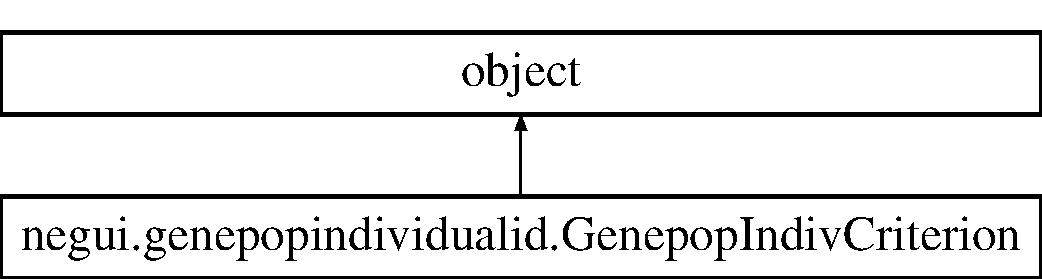
\includegraphics[height=2.000000cm]{classnegui_1_1genepopindividualid_1_1GenepopIndivCriterion}
\end{center}
\end{figure}
\subsection*{Public Member Functions}
\begin{DoxyCompactItemize}
\item 
def {\bfseries make\+\_\+test\+\_\+variable} (s\+\_\+field\+\_\+name)\hypertarget{classnegui_1_1genepopindividualid_1_1GenepopIndivCriterion_a2ab1a84a106514282b5c70a9033914c5}{}\label{classnegui_1_1genepopindividualid_1_1GenepopIndivCriterion_a2ab1a84a106514282b5c70a9033914c5}

\item 
def \hyperlink{classnegui_1_1genepopindividualid_1_1GenepopIndivCriterion_a58d025aa5c671e8c07fc9f0bbe56e588}{\+\_\+\+\_\+init\+\_\+\+\_\+} (self, s\+\_\+criterion\+\_\+name, ls\+\_\+field\+\_\+names, s\+\_\+test\+\_\+expression)
\item 
def \hyperlink{classnegui_1_1genepopindividualid_1_1GenepopIndivCriterion_a7f540e7e62b1c078ed06bb42a07f34f6}{do\+Test} (self, lv\+\_\+values)
\item 
def {\bfseries name} (self)\hypertarget{classnegui_1_1genepopindividualid_1_1GenepopIndivCriterion_a99d76ccf4421f71f84f2cbd4ecfad4f8}{}\label{classnegui_1_1genepopindividualid_1_1GenepopIndivCriterion_a99d76ccf4421f71f84f2cbd4ecfad4f8}

\item 
def {\bfseries name} (self, s\+\_\+name)\hypertarget{classnegui_1_1genepopindividualid_1_1GenepopIndivCriterion_a06866e0e47fa5269dcd20a6a576a56fb}{}\label{classnegui_1_1genepopindividualid_1_1GenepopIndivCriterion_a06866e0e47fa5269dcd20a6a576a56fb}

\item 
def {\bfseries fields} (self)\hypertarget{classnegui_1_1genepopindividualid_1_1GenepopIndivCriterion_abc0d0649b56e6e9fd578bf57941f717c}{}\label{classnegui_1_1genepopindividualid_1_1GenepopIndivCriterion_abc0d0649b56e6e9fd578bf57941f717c}

\item 
def {\bfseries fields} (self, ls\+\_\+fieldnames)\hypertarget{classnegui_1_1genepopindividualid_1_1GenepopIndivCriterion_a2ecc478307996482b6c5823475dbbad1}{}\label{classnegui_1_1genepopindividualid_1_1GenepopIndivCriterion_a2ecc478307996482b6c5823475dbbad1}

\item 
def {\bfseries test} (self)\hypertarget{classnegui_1_1genepopindividualid_1_1GenepopIndivCriterion_a002f19332a8434e4d1fba8be4d6d3134}{}\label{classnegui_1_1genepopindividualid_1_1GenepopIndivCriterion_a002f19332a8434e4d1fba8be4d6d3134}

\item 
def {\bfseries test} (self, s\+\_\+expression)\hypertarget{classnegui_1_1genepopindividualid_1_1GenepopIndivCriterion_a0b5653aacdb42c7f92fce358021c307b}{}\label{classnegui_1_1genepopindividualid_1_1GenepopIndivCriterion_a0b5653aacdb42c7f92fce358021c307b}

\end{DoxyCompactItemize}
\subsection*{Static Public Attributes}
\begin{DoxyCompactItemize}
\item 
string {\bfseries F\+I\+E\+L\+D\+\_\+\+D\+E\+L\+I\+M\+I\+T\+E\+R\+\_\+\+F\+O\+R\+\_\+\+T\+E\+S\+T\+\_\+\+E\+X\+P\+R\+E\+S\+S\+I\+ON} = \char`\"{}\%\char`\"{}\hypertarget{classnegui_1_1genepopindividualid_1_1GenepopIndivCriterion_a350c743f531d728cf22f760865c8329d}{}\label{classnegui_1_1genepopindividualid_1_1GenepopIndivCriterion_a350c743f531d728cf22f760865c8329d}

\end{DoxyCompactItemize}


\subsection{Detailed Description}
\begin{DoxyVerb}Class wraps a boolean test of one or more field
in a genepop file individual id.  Instances
of this class are members of a dictionary that
is used by class GenepopIndivCriteria, so that
a client can test the id against an number of
such criteria.
\end{DoxyVerb}
 

Definition at line 243 of file genepopindividualid.\+py.



\subsection{Constructor \& Destructor Documentation}
\index{negui\+::genepopindividualid\+::\+Genepop\+Indiv\+Criterion@{negui\+::genepopindividualid\+::\+Genepop\+Indiv\+Criterion}!\+\_\+\+\_\+init\+\_\+\+\_\+@{\+\_\+\+\_\+init\+\_\+\+\_\+}}
\index{\+\_\+\+\_\+init\+\_\+\+\_\+@{\+\_\+\+\_\+init\+\_\+\+\_\+}!negui\+::genepopindividualid\+::\+Genepop\+Indiv\+Criterion@{negui\+::genepopindividualid\+::\+Genepop\+Indiv\+Criterion}}
\subsubsection[{\texorpdfstring{\+\_\+\+\_\+init\+\_\+\+\_\+(self, s\+\_\+criterion\+\_\+name, ls\+\_\+field\+\_\+names, s\+\_\+test\+\_\+expression)}{__init__(self, s_criterion_name, ls_field_names, s_test_expression)}}]{\setlength{\rightskip}{0pt plus 5cm}def negui.\+genepopindividualid.\+Genepop\+Indiv\+Criterion.\+\_\+\+\_\+init\+\_\+\+\_\+ (
\begin{DoxyParamCaption}
\item[{}]{self, }
\item[{}]{s\+\_\+criterion\+\_\+name, }
\item[{}]{ls\+\_\+field\+\_\+names, }
\item[{}]{s\+\_\+test\+\_\+expression}
\end{DoxyParamCaption}
)}\hypertarget{classnegui_1_1genepopindividualid_1_1GenepopIndivCriterion_a58d025aa5c671e8c07fc9f0bbe56e588}{}\label{classnegui_1_1genepopindividualid_1_1GenepopIndivCriterion_a58d025aa5c671e8c07fc9f0bbe56e588}
\begin{DoxyVerb}param s_criterion_name, string giving a name for the
    criterion.  This name will be used by objects of
    class GenepopIndividualId as keys to a dictionary
    of instances of this class.
param s_field_names, list of strings, the ID field names to which the criteria
    is being applied.  These string should be present, surroundedused in the
    test expression (see next param).
param s_test_expression, string.  When evaluated, should generate
    True or False, as passing or failing the criterion's test.  The
    field name in this expression will be identified (field name surrounded
    by percent signs )and replaced by its value when
    this objects doTest() is called by the client, which passes the
    value in to the doTest def.  Example, if a field in the id stands
    for the individuals age, and is called "age", then the test expression might be, 
    "%age%==1".  When a client calls doTest, then, the "age" string will be replaced
    by the value, then eval will be called on the expression, and the boolean returned.
\end{DoxyVerb}
 

Definition at line 264 of file genepopindividualid.\+py.


\begin{DoxyCode}
264                             s\_test\_expression ):
265         \textcolor{stringliteral}{'''}
266 \textcolor{stringliteral}{        param s\_criterion\_name, string giving a name for the}
267 \textcolor{stringliteral}{            criterion.  This name will be used by objects of}
268 \textcolor{stringliteral}{            class GenepopIndividualId as keys to a dictionary}
269 \textcolor{stringliteral}{            of instances of this class.}
270 \textcolor{stringliteral}{        param s\_field\_names, list of strings, the ID field names to which the criteria}
271 \textcolor{stringliteral}{            is being applied.  These string should be present, surroundedused in the}
272 \textcolor{stringliteral}{            test expression (see next param).}
273 \textcolor{stringliteral}{        param s\_test\_expression, string.  When evaluated, should generate}
274 \textcolor{stringliteral}{            True or False, as passing or failing the criterion's test.  The}
275 \textcolor{stringliteral}{            field name in this expression will be identified (field name surrounded}
276 \textcolor{stringliteral}{            by percent signs )and replaced by its value when}
277 \textcolor{stringliteral}{            this objects doTest() is called by the client, which passes the}
278 \textcolor{stringliteral}{            value in to the doTest def.  Example, if a field in the id stands}
279 \textcolor{stringliteral}{            for the individuals age, and is called "age", then the test expression might be, }
280 \textcolor{stringliteral}{            "%age%==1".  When a client calls doTest, then, the "age" string will be replaced}
281 \textcolor{stringliteral}{            by the value, then eval will be called on the expression, and the boolean returned.}
282 \textcolor{stringliteral}{        '''}
283 
284         self.\hyperlink{classnegui_1_1genepopindividualid_1_1GenepopIndivCriterion_a94868409c57dda8cfcfd6cabf7554a10}{\_\_criterionname}=s\_criterion\_name
285         self.\hyperlink{classnegui_1_1genepopindividualid_1_1GenepopIndivCriterion_a490a6d671b1933addb37c32af20248c2}{\_\_fieldnames}=[ s\_name \textcolor{keywordflow}{for} s\_name \textcolor{keywordflow}{in} ls\_field\_names ]
286         self.\hyperlink{classnegui_1_1genepopindividualid_1_1GenepopIndivCriterion_a4366f9abf2851f4e83b62de2836ab812}{\_\_test}=s\_test\_expression
287         \textcolor{keywordflow}{return}
\end{DoxyCode}


\subsection{Member Function Documentation}
\index{negui\+::genepopindividualid\+::\+Genepop\+Indiv\+Criterion@{negui\+::genepopindividualid\+::\+Genepop\+Indiv\+Criterion}!do\+Test@{do\+Test}}
\index{do\+Test@{do\+Test}!negui\+::genepopindividualid\+::\+Genepop\+Indiv\+Criterion@{negui\+::genepopindividualid\+::\+Genepop\+Indiv\+Criterion}}
\subsubsection[{\texorpdfstring{do\+Test(self, lv\+\_\+values)}{doTest(self, lv_values)}}]{\setlength{\rightskip}{0pt plus 5cm}def negui.\+genepopindividualid.\+Genepop\+Indiv\+Criterion.\+do\+Test (
\begin{DoxyParamCaption}
\item[{}]{self, }
\item[{}]{lv\+\_\+values}
\end{DoxyParamCaption}
)}\hypertarget{classnegui_1_1genepopindividualid_1_1GenepopIndivCriterion_a7f540e7e62b1c078ed06bb42a07f34f6}{}\label{classnegui_1_1genepopindividualid_1_1GenepopIndivCriterion_a7f540e7e62b1c078ed06bb42a07f34f6}
\begin{DoxyVerb}See param definitions in __init__ for an example
and explanation of how this def works

We assume that the values are ordered in the arg list,
such that each nth value corresponds to the nth fields
in the list of field names.
\end{DoxyVerb}
 

Definition at line 290 of file genepopindividualid.\+py.


\begin{DoxyCode}
290     \textcolor{keyword}{def }\hyperlink{classnegui_1_1genepopindividualid_1_1GenepopIndivCriterion_a7f540e7e62b1c078ed06bb42a07f34f6}{doTest}( self, lv\_values ):
291         \textcolor{stringliteral}{'''}
292 \textcolor{stringliteral}{        See param definitions in \_\_init\_\_ for an example}
293 \textcolor{stringliteral}{        and explanation of how this def works}
294 \textcolor{stringliteral}{}
295 \textcolor{stringliteral}{        We assume that the values are ordered in the arg list,}
296 \textcolor{stringliteral}{        such that each nth value corresponds to the nth fields}
297 \textcolor{stringliteral}{        in the list of field names.}
298 \textcolor{stringliteral}{        '''}
299         \textcolor{comment}{#make sure we have exactly one value for each field}
300 
301         i\_num\_vals=len( lv\_values )
302         i\_num\_fieldnames=len( self.\hyperlink{classnegui_1_1genepopindividualid_1_1GenepopIndivCriterion_a490a6d671b1933addb37c32af20248c2}{\_\_fieldnames} )
303 
304         \textcolor{keywordflow}{if} i\_num\_vals != i\_num\_fieldnames:
305             s\_msg=\textcolor{stringliteral}{"In GenepopIndivCriterion instance, def doTest, "} \(\backslash\)
306                         + \textcolor{stringliteral}{"number of values passed in as arg, "} \(\backslash\)
307                         + str( i\_num\_vals ) + \textcolor{stringliteral}{" does not equal "} \(\backslash\)
308                         + \textcolor{stringliteral}{"the number of field names, "} \(\backslash\)
309                         + \textcolor{stringliteral}{"for this criterion, "} \(\backslash\)
310                         + str( i\_num\_fieldnames ) + \textcolor{stringliteral}{"."} \(\backslash\)
311                         + \textcolor{stringliteral}{"Field name list: "} + str( self.\hyperlink{classnegui_1_1genepopindividualid_1_1GenepopIndivCriterion_a490a6d671b1933addb37c32af20248c2}{\_\_fieldnames} ) \(\backslash\)
312                         + \textcolor{stringliteral}{".  Value list: "} + str( lv\_values ) + \textcolor{stringliteral}{"."}
313             \textcolor{keywordflow}{raise} Exception( s\_msg )
314         \textcolor{comment}{#end if num fields not equal num vals}
315 
316         v\_result=\textcolor{keywordtype}{None}
317 
318         ls\_field\_vars=[]
319         lv\_vetted\_field\_vals=[]
320 
321         \textcolor{comment}{#convert field names to their variable form}
322         \textcolor{comment}{#as used in the test:}
323         \textcolor{keywordflow}{for} s\_field\_name \textcolor{keywordflow}{in} self.\hyperlink{classnegui_1_1genepopindividualid_1_1GenepopIndivCriterion_a490a6d671b1933addb37c32af20248c2}{\_\_fieldnames}:
324 
325             s\_field\_variable= \(\backslash\)
326                     GenepopIndivCriterion.FIELD\_DELIMITER\_FOR\_TEST\_EXPRESSION \(\backslash\)
327                     + s\_field\_name \(\backslash\)
328                     + GenepopIndivCriterion.FIELD\_DELIMITER\_FOR\_TEST\_EXPRESSION
329 
330             \textcolor{comment}{#Make sure the test expression includes}
331             \textcolor{comment}{#the field name surrounded by quotes:}
332             \textcolor{keywordflow}{if} s\_field\_variable  \textcolor{keywordflow}{not} \textcolor{keywordflow}{in} self.\hyperlink{classnegui_1_1genepopindividualid_1_1GenepopIndivCriterion_a4366f9abf2851f4e83b62de2836ab812}{\_\_test}:
333                 s\_msg=\textcolor{stringliteral}{"In GenepopIndivCriterion instance, "} \(\backslash\)
334                         + \textcolor{stringliteral}{"test expression: "} + self.\hyperlink{classnegui_1_1genepopindividualid_1_1GenepopIndivCriterion_a4366f9abf2851f4e83b62de2836ab812}{\_\_test} \(\backslash\)
335                         + \textcolor{stringliteral}{" does not contain the field-name string for substitution: "} \(\backslash\)
336                         + s\_field\_name + \textcolor{stringliteral}{"."}
337                 \textcolor{keywordflow}{raise} Exception( s\_msg )
338             \textcolor{comment}{#end if sub string not present in test expression}
339 
340             ls\_field\_vars.append( s\_field\_variable )
341 
342         \textcolor{comment}{#end for each field name}
343         
344         \textcolor{comment}{#as required put string values in quotes:}
345         \textcolor{keywordflow}{for} v\_value \textcolor{keywordflow}{in} lv\_values:
346             \textcolor{keywordflow}{if} type( v\_value ) == str:
347                 v\_value=\textcolor{stringliteral}{"\(\backslash\)""} + v\_value + \textcolor{stringliteral}{"\(\backslash\)""}
348             \textcolor{comment}{#end if value is a string, add quotes for eval}
349 
350             lv\_vetted\_field\_vals.append( v\_value )
351         \textcolor{comment}{#end for each value, check if quotes needed}
352     
353         \textcolor{comment}{#we iterively replace the variables with their}
354         \textcolor{comment}{#values}
355         s\_test\_with\_val=self.\hyperlink{classnegui_1_1genepopindividualid_1_1GenepopIndivCriterion_a4366f9abf2851f4e83b62de2836ab812}{\_\_test}
356     
357         \textcolor{keywordflow}{for} idx \textcolor{keywordflow}{in} range( len( ls\_field\_vars ) ):
358 
359             s\_field\_variable=ls\_field\_vars[ idx ]
360             v\_vetted\_field\_val=lv\_vetted\_field\_vals[ idx ]
361             s\_test\_with\_val=s\_test\_with\_val.replace( s\_field\_variable, str( v\_vetted\_field\_val ) )
362 
363         \textcolor{keywordflow}{try}:
364             v\_result=eval( s\_test\_with\_val )    
365         \textcolor{keywordflow}{except} Exception \textcolor{keyword}{as} oex:
366             s\_msg=\textcolor{stringliteral}{"In GenepopIndivCriterion instance, "} \(\backslash\)
367                     + \textcolor{stringliteral}{"eval of test failed.  Test: "} \(\backslash\)
368                     + s\_test\_with\_val \(\backslash\)
369                     + \textcolor{stringliteral}{".  Eval raised exception: "} \(\backslash\)
370                     + str( oex ) + \textcolor{stringliteral}{"."}
371             \textcolor{keywordflow}{raise} Exception ( s\_msg )
372         \textcolor{comment}{#end try...except}
373 
374         \textcolor{keywordflow}{if} v\_result \textcolor{keywordflow}{not} \textcolor{keywordflow}{in} [ \textcolor{keyword}{True}, \textcolor{keyword}{False} ]:
375             s\_msg = \textcolor{stringliteral}{"In GenepopIndivCriterion instance, def doTest, "} \(\backslash\)
376                             + \textcolor{stringliteral}{"test returned non-boolean value: "} + str( v\_result ) \(\backslash\)
377                             + \textcolor{stringliteral}{".  Boolean value is required."}
378             \textcolor{keywordflow}{raise} Exception( s\_msg )
379         \textcolor{comment}{#end if v\_result not boolean}
380 
381         \textcolor{keywordflow}{return} v\_result
\end{DoxyCode}


The documentation for this class was generated from the following file\+:\begin{DoxyCompactItemize}
\item 
genepopindividualid.\+py\end{DoxyCompactItemize}

\hypertarget{classnegui_1_1genepopindividualid_1_1GenepopIndivIdAgeStructure}{}\section{negui.\+genepopindividualid.\+Genepop\+Indiv\+Id\+Age\+Structure Class Reference}
\label{classnegui_1_1genepopindividualid_1_1GenepopIndivIdAgeStructure}\index{negui.\+genepopindividualid.\+Genepop\+Indiv\+Id\+Age\+Structure@{negui.\+genepopindividualid.\+Genepop\+Indiv\+Id\+Age\+Structure}}
Inheritance diagram for negui.\+genepopindividualid.\+Genepop\+Indiv\+Id\+Age\+Structure\+:\begin{figure}[H]
\begin{center}
\leavevmode
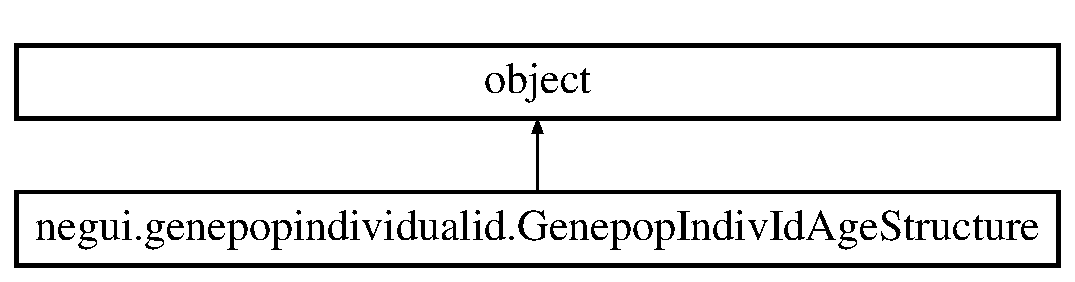
\includegraphics[height=2.000000cm]{classnegui_1_1genepopindividualid_1_1GenepopIndivIdAgeStructure}
\end{center}
\end{figure}
\subsection*{Public Member Functions}
\begin{DoxyCompactItemize}
\item 
def {\bfseries \+\_\+\+\_\+init\+\_\+\+\_\+} (self, s\+\_\+id)\hypertarget{classnegui_1_1genepopindividualid_1_1GenepopIndivIdAgeStructure_a9135a344dc50b0452eca7b226d7bd0fd}{}\label{classnegui_1_1genepopindividualid_1_1GenepopIndivIdAgeStructure_a9135a344dc50b0452eca7b226d7bd0fd}

\end{DoxyCompactItemize}
\subsection*{Static Public Attributes}
\begin{DoxyCompactItemize}
\item 
string {\bfseries D\+E\+L\+I\+M\+I\+T\+E\+R\+\_\+\+F\+I\+E\+L\+DS} = \char`\"{};\char`\"{}\hypertarget{classnegui_1_1genepopindividualid_1_1GenepopIndivIdAgeStructure_aecc9bfba2087710aceb8bd3ef9b4141a}{}\label{classnegui_1_1genepopindividualid_1_1GenepopIndivIdAgeStructure_aecc9bfba2087710aceb8bd3ef9b4141a}

\item 
int {\bfseries I\+D\+X\+\_\+\+ID} = 0\hypertarget{classnegui_1_1genepopindividualid_1_1GenepopIndivIdAgeStructure_afbe562b1188b505d8344b8ee954505d8}{}\label{classnegui_1_1genepopindividualid_1_1GenepopIndivIdAgeStructure_afbe562b1188b505d8344b8ee954505d8}

\item 
int {\bfseries I\+D\+X\+\_\+\+S\+EX} = 1\hypertarget{classnegui_1_1genepopindividualid_1_1GenepopIndivIdAgeStructure_a181691e25e7dd54443c86570e3445c4c}{}\label{classnegui_1_1genepopindividualid_1_1GenepopIndivIdAgeStructure_a181691e25e7dd54443c86570e3445c4c}

\item 
int {\bfseries I\+D\+X\+\_\+\+F\+A\+T\+H\+ER} = 2\hypertarget{classnegui_1_1genepopindividualid_1_1GenepopIndivIdAgeStructure_a049294a5df9e6fef713e378089058a23}{}\label{classnegui_1_1genepopindividualid_1_1GenepopIndivIdAgeStructure_a049294a5df9e6fef713e378089058a23}

\item 
int {\bfseries I\+D\+X\+\_\+\+M\+O\+T\+H\+ER} = 3\hypertarget{classnegui_1_1genepopindividualid_1_1GenepopIndivIdAgeStructure_ac0a84685cdad11327e3e89bf966a27ec}{}\label{classnegui_1_1genepopindividualid_1_1GenepopIndivIdAgeStructure_ac0a84685cdad11327e3e89bf966a27ec}

\item 
int {\bfseries I\+D\+X\+\_\+\+A\+GE} = 4\hypertarget{classnegui_1_1genepopindividualid_1_1GenepopIndivIdAgeStructure_aa782c2cf26fbde653c63a5f861bd91ab}{}\label{classnegui_1_1genepopindividualid_1_1GenepopIndivIdAgeStructure_aa782c2cf26fbde653c63a5f861bd91ab}

\item 
int {\bfseries T\+O\+T\+A\+L\+\_\+\+F\+I\+E\+L\+DS} = 5\hypertarget{classnegui_1_1genepopindividualid_1_1GenepopIndivIdAgeStructure_a0a2c518fe0454a8616bfffd87d4d75aa}{}\label{classnegui_1_1genepopindividualid_1_1GenepopIndivIdAgeStructure_a0a2c518fe0454a8616bfffd87d4d75aa}

\end{DoxyCompactItemize}


\subsection{Detailed Description}
\begin{DoxyVerb}Wraps the individual ID's as found in genepop
files as output by objects of class PGOutputSimuPop
\end{DoxyVerb}
 

Definition at line 15 of file genepopindividualid.\+py.



The documentation for this class was generated from the following file\+:\begin{DoxyCompactItemize}
\item 
genepopindividualid.\+py\end{DoxyCompactItemize}

\hypertarget{classnegui_1_1genepopindividualid_1_1GenepopIndivIdFields}{}\section{negui.\+genepopindividualid.\+Genepop\+Indiv\+Id\+Fields Class Reference}
\label{classnegui_1_1genepopindividualid_1_1GenepopIndivIdFields}\index{negui.\+genepopindividualid.\+Genepop\+Indiv\+Id\+Fields@{negui.\+genepopindividualid.\+Genepop\+Indiv\+Id\+Fields}}
Inheritance diagram for negui.\+genepopindividualid.\+Genepop\+Indiv\+Id\+Fields\+:\begin{figure}[H]
\begin{center}
\leavevmode
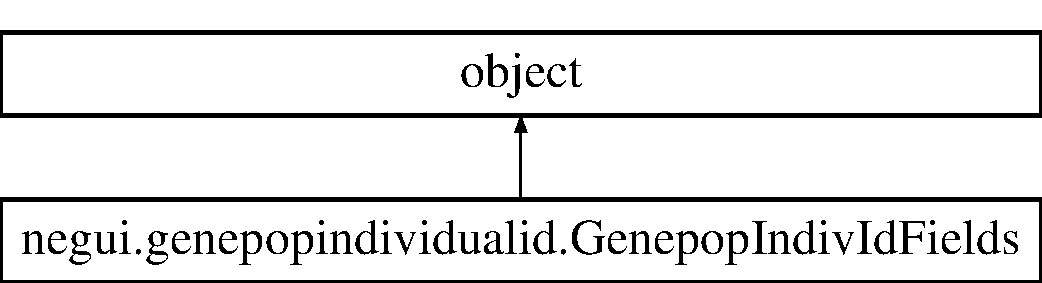
\includegraphics[height=2.000000cm]{classnegui_1_1genepopindividualid_1_1GenepopIndivIdFields}
\end{center}
\end{figure}
\subsection*{Public Member Functions}
\begin{DoxyCompactItemize}
\item 
def {\bfseries \+\_\+\+\_\+init\+\_\+\+\_\+} (self, ls\+\_\+field\+\_\+names=\mbox{[}\char`\"{}number\char`\"{}\mbox{]}, lo\+\_\+field\+\_\+types=\mbox{[}int\mbox{]})\hypertarget{classnegui_1_1genepopindividualid_1_1GenepopIndivIdFields_a76e45449d1c5386efcaadbabaa8e7dc0}{}\label{classnegui_1_1genepopindividualid_1_1GenepopIndivIdFields_a76e45449d1c5386efcaadbabaa8e7dc0}

\item 
def {\bfseries types} (self)\hypertarget{classnegui_1_1genepopindividualid_1_1GenepopIndivIdFields_a45ccbceb841638d3a9cedaa1d220137b}{}\label{classnegui_1_1genepopindividualid_1_1GenepopIndivIdFields_a45ccbceb841638d3a9cedaa1d220137b}

\item 
def {\bfseries names} (self)\hypertarget{classnegui_1_1genepopindividualid_1_1GenepopIndivIdFields_aed28d052aaddf07f914bb9190f8be737}{}\label{classnegui_1_1genepopindividualid_1_1GenepopIndivIdFields_aed28d052aaddf07f914bb9190f8be737}

\end{DoxyCompactItemize}


\subsection{Detailed Description}


Definition at line 119 of file genepopindividualid.\+py.



The documentation for this class was generated from the following file\+:\begin{DoxyCompactItemize}
\item 
genepopindividualid.\+py\end{DoxyCompactItemize}

\hypertarget{classnegui_1_1genepopindividualid_1_1GenepopIndividualId}{}\section{negui.\+genepopindividualid.\+Genepop\+Individual\+Id Class Reference}
\label{classnegui_1_1genepopindividualid_1_1GenepopIndividualId}\index{negui.\+genepopindividualid.\+Genepop\+Individual\+Id@{negui.\+genepopindividualid.\+Genepop\+Individual\+Id}}
Inheritance diagram for negui.\+genepopindividualid.\+Genepop\+Individual\+Id\+:\begin{figure}[H]
\begin{center}
\leavevmode
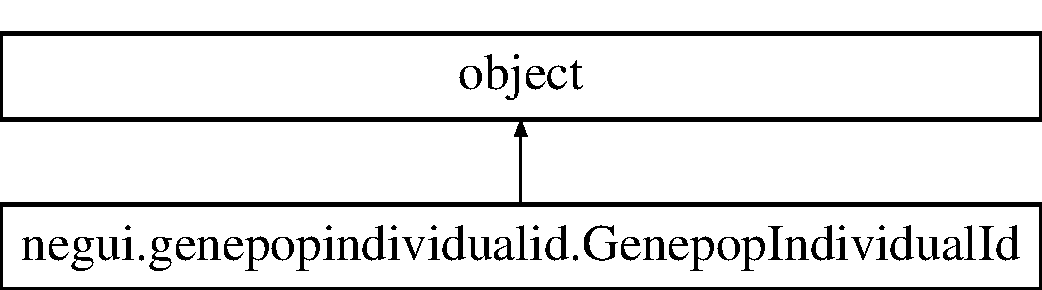
\includegraphics[height=2.000000cm]{classnegui_1_1genepopindividualid_1_1GenepopIndividualId}
\end{center}
\end{figure}
\subsection*{Public Member Functions}
\begin{DoxyCompactItemize}
\item 
def {\bfseries \+\_\+\+\_\+init\+\_\+\+\_\+} (self, o\+\_\+genepop\+\_\+indiv\+\_\+vals, o\+\_\+genepop\+\_\+criteria=None)\hypertarget{classnegui_1_1genepopindividualid_1_1GenepopIndividualId_a6a5d9b3214414313abf23acdea0e8dbc}{}\label{classnegui_1_1genepopindividualid_1_1GenepopIndividualId_a6a5d9b3214414313abf23acdea0e8dbc}

\item 
def \hyperlink{classnegui_1_1genepopindividualid_1_1GenepopIndividualId_ab25e0ae796fa9574369af186b1e2e6c0}{all\+Criteria\+Are\+True} (self)
\end{DoxyCompactItemize}


\subsection{Detailed Description}
\begin{DoxyVerb}Wraps genepop indiv. ids as
represented by member class instances
of GenepopIndivIdFields and GenepopIndivCriteria
\end{DoxyVerb}
 

Definition at line 551 of file genepopindividualid.\+py.



\subsection{Member Function Documentation}
\index{negui\+::genepopindividualid\+::\+Genepop\+Individual\+Id@{negui\+::genepopindividualid\+::\+Genepop\+Individual\+Id}!all\+Criteria\+Are\+True@{all\+Criteria\+Are\+True}}
\index{all\+Criteria\+Are\+True@{all\+Criteria\+Are\+True}!negui\+::genepopindividualid\+::\+Genepop\+Individual\+Id@{negui\+::genepopindividualid\+::\+Genepop\+Individual\+Id}}
\subsubsection[{\texorpdfstring{all\+Criteria\+Are\+True(self)}{allCriteriaAreTrue(self)}}]{\setlength{\rightskip}{0pt plus 5cm}def negui.\+genepopindividualid.\+Genepop\+Individual\+Id.\+all\+Criteria\+Are\+True (
\begin{DoxyParamCaption}
\item[{}]{self}
\end{DoxyParamCaption}
)}\hypertarget{classnegui_1_1genepopindividualid_1_1GenepopIndividualId_ab25e0ae796fa9574369af186b1e2e6c0}{}\label{classnegui_1_1genepopindividualid_1_1GenepopIndividualId_ab25e0ae796fa9574369af186b1e2e6c0}
\begin{DoxyVerb}Returns True if there are no
criteria, otherwise the "and"
operation of all criteria tests
(see class GenepopIndivCriteria).
\end{DoxyVerb}
 

Definition at line 577 of file genepopindividualid.\+py.


\begin{DoxyCode}
577     \textcolor{keyword}{def }\hyperlink{classnegui_1_1genepopindividualid_1_1GenepopIndividualId_ab25e0ae796fa9574369af186b1e2e6c0}{allCriteriaAreTrue}( self ):
578         \textcolor{stringliteral}{'''}
579 \textcolor{stringliteral}{        Returns True if there are no}
580 \textcolor{stringliteral}{        criteria, otherwise the "and"}
581 \textcolor{stringliteral}{        operation of all criteria tests}
582 \textcolor{stringliteral}{        (see class GenepopIndivCriteria).}
583 \textcolor{stringliteral}{        '''}
584         b\_result=\textcolor{keyword}{True}
585         ls\_field\_names=self.\_\_values.fieldnames
586         lv\_field\_values=[]
587         \textcolor{keywordflow}{if} self.\hyperlink{classnegui_1_1genepopindividualid_1_1GenepopIndividualId_a2052378559bc94b76c8d59a51819ad24}{\_\_criteria} \textcolor{keywordflow}{is} \textcolor{keywordflow}{not} \textcolor{keywordtype}{None}:
588             \textcolor{keywordflow}{for} s\_field \textcolor{keywordflow}{in} ls\_field\_names:              
589                 lv\_field\_values.append( \(\backslash\)
590                         self.\_\_values.getVal( s\_field ) )
591             \textcolor{comment}{#end for each field, get value}
592             
593             b\_result=self.\_\_criteria.allTestsAreTrue( \(\backslash\)
594                             ls\_field\_names, lv\_field\_values )
595         \textcolor{comment}{#end if we have criteria to test}
596 
597         \textcolor{keywordflow}{return} b\_result
\end{DoxyCode}


The documentation for this class was generated from the following file\+:\begin{DoxyCompactItemize}
\item 
genepopindividualid.\+py\end{DoxyCompactItemize}

\hypertarget{classnegui_1_1genepopindividualid_1_1GenepopIndivIdVals}{}\section{negui.\+genepopindividualid.\+Genepop\+Indiv\+Id\+Vals Class Reference}
\label{classnegui_1_1genepopindividualid_1_1GenepopIndivIdVals}\index{negui.\+genepopindividualid.\+Genepop\+Indiv\+Id\+Vals@{negui.\+genepopindividualid.\+Genepop\+Indiv\+Id\+Vals}}
Inheritance diagram for negui.\+genepopindividualid.\+Genepop\+Indiv\+Id\+Vals\+:\begin{figure}[H]
\begin{center}
\leavevmode
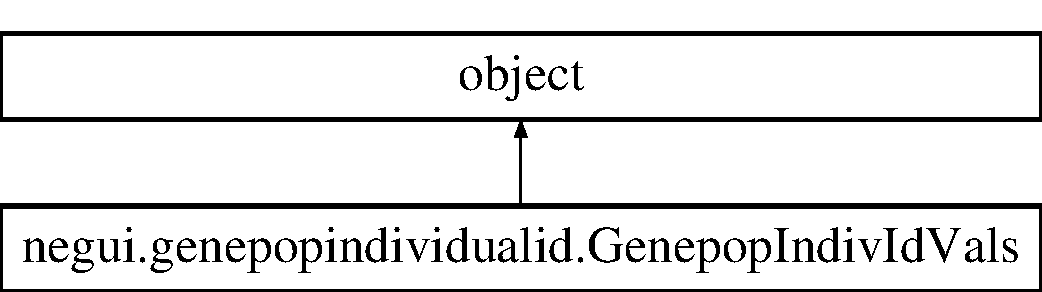
\includegraphics[height=2.000000cm]{classnegui_1_1genepopindividualid_1_1GenepopIndivIdVals}
\end{center}
\end{figure}
\subsection*{Public Member Functions}
\begin{DoxyCompactItemize}
\item 
def {\bfseries \+\_\+\+\_\+init\+\_\+\+\_\+} (self, s\+\_\+id, o\+\_\+genepop\+\_\+indiv\+\_\+fields, s\+\_\+delimiter=\char`\"{};\char`\"{})\hypertarget{classnegui_1_1genepopindividualid_1_1GenepopIndivIdVals_a72145be2e4d8a444567c89818f3c0814}{}\label{classnegui_1_1genepopindividualid_1_1GenepopIndivIdVals_a72145be2e4d8a444567c89818f3c0814}

\item 
def {\bfseries get\+Val} (self, s\+\_\+name)\hypertarget{classnegui_1_1genepopindividualid_1_1GenepopIndivIdVals_a603565db54797a7551e4632b9d3442b3}{}\label{classnegui_1_1genepopindividualid_1_1GenepopIndivIdVals_a603565db54797a7551e4632b9d3442b3}

\item 
def {\bfseries fieldnames} (self)\hypertarget{classnegui_1_1genepopindividualid_1_1GenepopIndivIdVals_af40421346609ca97846993710f086802}{}\label{classnegui_1_1genepopindividualid_1_1GenepopIndivIdVals_af40421346609ca97846993710f086802}

\end{DoxyCompactItemize}


\subsection{Detailed Description}


Definition at line 158 of file genepopindividualid.\+py.



The documentation for this class was generated from the following file\+:\begin{DoxyCompactItemize}
\item 
genepopindividualid.\+py\end{DoxyCompactItemize}

\hypertarget{classnegui_1_1pgutilityclasses_1_1GenepopPopWriter}{}\section{negui.\+pgutilityclasses.\+Genepop\+Pop\+Writer Class Reference}
\label{classnegui_1_1pgutilityclasses_1_1GenepopPopWriter}\index{negui.\+pgutilityclasses.\+Genepop\+Pop\+Writer@{negui.\+pgutilityclasses.\+Genepop\+Pop\+Writer}}
Inheritance diagram for negui.\+pgutilityclasses.\+Genepop\+Pop\+Writer\+:\begin{figure}[H]
\begin{center}
\leavevmode
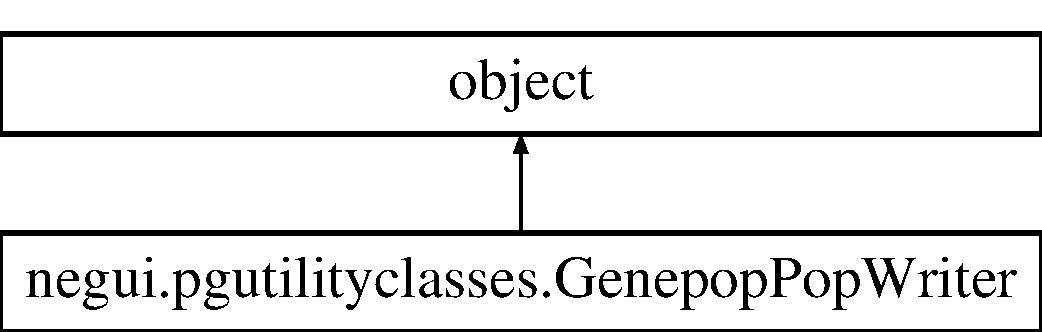
\includegraphics[height=2.000000cm]{classnegui_1_1pgutilityclasses_1_1GenepopPopWriter}
\end{center}
\end{figure}
\subsection*{Public Member Functions}
\begin{DoxyCompactItemize}
\item 
def {\bfseries \+\_\+\+\_\+init\+\_\+\+\_\+} (self, s\+\_\+genepop\+\_\+file\+\_\+name, s\+\_\+header, s\+\_\+loci\+\_\+lines, i\+\_\+max\+\_\+entry\+\_\+capacity=S\+T\+A\+N\+D\+A\+R\+D\+\_\+\+C\+A\+P\+A\+C\+I\+TY)\hypertarget{classnegui_1_1pgutilityclasses_1_1GenepopPopWriter_ab959b06f8c41bcbc7615144cd1f25ed7}{}\label{classnegui_1_1pgutilityclasses_1_1GenepopPopWriter_ab959b06f8c41bcbc7615144cd1f25ed7}

\item 
def \hyperlink{classnegui_1_1pgutilityclasses_1_1GenepopPopWriter_a5c7d53c68d1c3533ed1fd861f9bd60e4}{add\+Entry\+And\+Write\+First\+If\+Full} (self, i\+\_\+pop\+\_\+number, s\+\_\+indiv\+\_\+and\+\_\+loci\+\_\+entry)
\item 
def {\bfseries entry\+\_\+count} (self)\hypertarget{classnegui_1_1pgutilityclasses_1_1GenepopPopWriter_aed8c87c59012a83d0b8aa02f0c06b8fc}{}\label{classnegui_1_1pgutilityclasses_1_1GenepopPopWriter_aed8c87c59012a83d0b8aa02f0c06b8fc}

\end{DoxyCompactItemize}
\subsection*{Static Public Attributes}
\begin{DoxyCompactItemize}
\item 
int {\bfseries S\+T\+A\+N\+D\+A\+R\+D\+\_\+\+C\+A\+P\+A\+C\+I\+TY} = 1\hypertarget{classnegui_1_1pgutilityclasses_1_1GenepopPopWriter_a079997944121d92a315f774cae76ff22}{}\label{classnegui_1_1pgutilityclasses_1_1GenepopPopWriter_a079997944121d92a315f774cae76ff22}

\end{DoxyCompactItemize}


\subsection{Detailed Description}
\begin{DoxyVerb}This class was created to simplify
and speed up the output performance 
of the simulation.  It is an alternative
to the original 3-file output that I conserved
from the original AgeStructure code.  

This class is meant to be used by PGOpSimuPop instances,
and the PGOutputSimuPop instances,
to store output until a threshold is reached, when it
will then write it to file.  

Assumtions 
  1. The client adds entries using numbering with ints the "pop" sections
    in the order they are intended to be written to file. 
  2.  The client adds entries in the order they are to be written.
  3.  The loci list is either \n endlined, or on a single line.

As of 2017_04_22 it is not yet integrated into the
simulation code.
\end{DoxyVerb}
 

Definition at line 1487 of file pgutilityclasses.\+py.



\subsection{Member Function Documentation}
\index{negui\+::pgutilityclasses\+::\+Genepop\+Pop\+Writer@{negui\+::pgutilityclasses\+::\+Genepop\+Pop\+Writer}!add\+Entry\+And\+Write\+First\+If\+Full@{add\+Entry\+And\+Write\+First\+If\+Full}}
\index{add\+Entry\+And\+Write\+First\+If\+Full@{add\+Entry\+And\+Write\+First\+If\+Full}!negui\+::pgutilityclasses\+::\+Genepop\+Pop\+Writer@{negui\+::pgutilityclasses\+::\+Genepop\+Pop\+Writer}}
\subsubsection[{\texorpdfstring{add\+Entry\+And\+Write\+First\+If\+Full(self, i\+\_\+pop\+\_\+number, s\+\_\+indiv\+\_\+and\+\_\+loci\+\_\+entry)}{addEntryAndWriteFirstIfFull(self, i_pop_number, s_indiv_and_loci_entry)}}]{\setlength{\rightskip}{0pt plus 5cm}def negui.\+pgutilityclasses.\+Genepop\+Pop\+Writer.\+add\+Entry\+And\+Write\+First\+If\+Full (
\begin{DoxyParamCaption}
\item[{}]{self, }
\item[{}]{i\+\_\+pop\+\_\+number, }
\item[{}]{s\+\_\+indiv\+\_\+and\+\_\+loci\+\_\+entry}
\end{DoxyParamCaption}
)}\hypertarget{classnegui_1_1pgutilityclasses_1_1GenepopPopWriter_a5c7d53c68d1c3533ed1fd861f9bd60e4}{}\label{classnegui_1_1pgutilityclasses_1_1GenepopPopWriter_a5c7d53c68d1c3533ed1fd861f9bd60e4}
\begin{DoxyVerb}This def checks the current capacity, and if the number of entries 
currently meets it, it will write the current pops to the file
given by the self.__genepop_file string.

Otherwise it will add the entry to the pop indicated by arg i_pop_number.
\end{DoxyVerb}
 

Definition at line 1578 of file pgutilityclasses.\+py.


\begin{DoxyCode}
1578     \textcolor{keyword}{def }\hyperlink{classnegui_1_1pgutilityclasses_1_1GenepopPopWriter_a5c7d53c68d1c3533ed1fd861f9bd60e4}{addEntryAndWriteFirstIfFull}( self, i\_pop\_number, s\_indiv\_and\_loci\_entry 
      ):
1579         \textcolor{stringliteral}{'''}
1580 \textcolor{stringliteral}{        This def checks the current capacity, and if the number of entries }
1581 \textcolor{stringliteral}{        currently meets it, it will write the current pops to the file}
1582 \textcolor{stringliteral}{        given by the self.\_\_genepop\_file string.}
1583 \textcolor{stringliteral}{}
1584 \textcolor{stringliteral}{        Otherwise it will add the entry to the pop indicated by arg i\_pop\_number.}
1585 \textcolor{stringliteral}{        '''}
1586 
1587         \textcolor{keywordflow}{if} self.\hyperlink{classnegui_1_1pgutilityclasses_1_1GenepopPopWriter_a304e157063ad06904e141c994c5b514f}{\_\_entry\_count} > i\_max\_entry\_capacity:
1588             s\_msg=\textcolor{stringliteral}{"In GenepopPopWriter instance, the current total "} \(\backslash\)
1589                         + \textcolor{stringliteral}{"for number of entries, "} + str( self.\hyperlink{classnegui_1_1pgutilityclasses_1_1GenepopPopWriter_a304e157063ad06904e141c994c5b514f}{\_\_entry\_count} ) \(\backslash\)
1590                         + \textcolor{stringliteral}{"exceeds the value for maximum capacity, "} \(\backslash\)
1591                         + str( self.\hyperlink{classnegui_1_1pgutilityclasses_1_1GenepopPopWriter_ac04999010b2eda1fbfc0c36cdac4943c}{\_\_max\_capacity} ) + \textcolor{stringliteral}{"."}
1592         \textcolor{keywordflow}{elif} self.\hyperlink{classnegui_1_1pgutilityclasses_1_1GenepopPopWriter_a304e157063ad06904e141c994c5b514f}{\_\_entry\_count}==i\_max\_entry\_capacity:
1593             self.\hyperlink{classnegui_1_1pgutilityclasses_1_1GenepopPopWriter_a5cc6479ab88e930a41d03b589397d241}{\_\_write\_current\_pop\_entries}
1594         \textcolor{keywordflow}{else}:
1595             b\_pop\_already\_written\_and\_surpassed = \(\backslash\)
1596                 i\_pop\_number \textcolor{keywordflow}{in} self.\hyperlink{classnegui_1_1pgutilityclasses_1_1GenepopPopWriter_a9ee4e3161f6698084fcf0d2ab747bd80}{\_\_numbers\_of\_written\_pops} \(\backslash\)
1597                     \textcolor{keywordflow}{and} i\_pop\_number != self.\hyperlink{classnegui_1_1pgutilityclasses_1_1GenepopPopWriter_ae11fb07e14cea411fd205f014cd75474}{\_\_num\_last\_pop\_written}
1598             b\_pop\_number\_smaller\_than\_current = \(\backslash\)
1599                 i\_pop\_number < self.\hyperlink{classnegui_1_1pgutilityclasses_1_1GenepopPopWriter_ae11fb07e14cea411fd205f014cd75474}{\_\_num\_last\_pop\_written}
1600             \textcolor{keywordflow}{if} b\_pop\_already\_written\_and\_surpassed \(\backslash\)
1601                     \textcolor{keywordflow}{or} b\_pop\_number\_smaller\_than\_current:
1602                 s\_msg=\textcolor{stringliteral}{"In GenepopPopWriter instance, the current entry, "} \(\backslash\)
1603                             + \textcolor{stringliteral}{"cannot be added.  It has a pop number, "}  \(\backslash\)
1604                             + str( i\_pop\_number ) \(\backslash\)
1605                             + \textcolor{stringliteral}{"lower than the last one written,  "} \(\backslash\)
1606                             + \textcolor{stringliteral}{"with other pops written after it."}
1607                 \textcolor{keywordflow}{raise} Exception( s\_msg )
1608             \textcolor{keywordflow}{else}:
1609                 \textcolor{keywordflow}{if} i\_pop \textcolor{keywordflow}{not} \textcolor{keywordflow}{in} self.\hyperlink{classnegui_1_1pgutilityclasses_1_1GenepopPopWriter_afa7ef2e505b37a1dff9bb3479c356df8}{\_\_pops}:
1610                     self.\hyperlink{classnegui_1_1pgutilityclasses_1_1GenepopPopWriter_afa7ef2e505b37a1dff9bb3479c356df8}{\_\_pops}[ i ]=[ s\_indiv\_and\_loci\_entry ]
1611                 \textcolor{keywordflow}{else}:
1612                     self.\hyperlink{classnegui_1_1pgutilityclasses_1_1GenepopPopWriter_afa7ef2e505b37a1dff9bb3479c356df8}{\_\_pops}[ i ].append( s\_indiv\_and\_loci\_entry )
1613                 \textcolor{comment}{#end}
1614                 \textcolor{stringliteral}{'''}
1615 \textcolor{stringliteral}{                This should be the only code that increments the}
1616 \textcolor{stringliteral}{                entry count. Note that it is decremented only in}
1617 \textcolor{stringliteral}{                \_\_write\_current\_pop\_entries.}
1618 \textcolor{stringliteral}{                '''}
1619                 self.\hyperlink{classnegui_1_1pgutilityclasses_1_1GenepopPopWriter_a304e157063ad06904e141c994c5b514f}{\_\_entry\_count} += 1
1620                     
1621             \textcolor{comment}{#end if pop has a number showing its either out of order}
1622             \textcolor{comment}{#or already written}
1623 
\end{DoxyCode}


The documentation for this class was generated from the following file\+:\begin{DoxyCompactItemize}
\item 
pgutilityclasses.\+py\end{DoxyCompactItemize}

\hypertarget{classnegui_1_1pgutilityclasses_1_1IndependantProcessGroup}{}\section{negui.\+pgutilityclasses.\+Independant\+Process\+Group Class Reference}
\label{classnegui_1_1pgutilityclasses_1_1IndependantProcessGroup}\index{negui.\+pgutilityclasses.\+Independant\+Process\+Group@{negui.\+pgutilityclasses.\+Independant\+Process\+Group}}
Inheritance diagram for negui.\+pgutilityclasses.\+Independant\+Process\+Group\+:\begin{figure}[H]
\begin{center}
\leavevmode
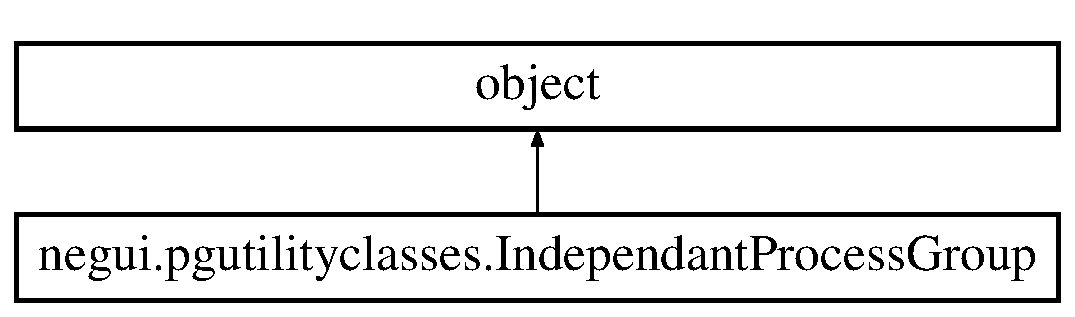
\includegraphics[height=2.000000cm]{classnegui_1_1pgutilityclasses_1_1IndependantProcessGroup}
\end{center}
\end{figure}
\subsection*{Public Member Functions}
\begin{DoxyCompactItemize}
\item 
def {\bfseries \+\_\+\+\_\+init\+\_\+\+\_\+} (self, lo\+\_\+processes=\mbox{[}$\,$\mbox{]})\hypertarget{classnegui_1_1pgutilityclasses_1_1IndependantProcessGroup_a5a2b256aa2b103efa417acf0a81a7f79}{}\label{classnegui_1_1pgutilityclasses_1_1IndependantProcessGroup_a5a2b256aa2b103efa417acf0a81a7f79}

\item 
def {\bfseries add\+Process} (self, o\+\_\+process)\hypertarget{classnegui_1_1pgutilityclasses_1_1IndependantProcessGroup_a71d901e440fa95a6c225c1c940e0f77c}{}\label{classnegui_1_1pgutilityclasses_1_1IndependantProcessGroup_a71d901e440fa95a6c225c1c940e0f77c}

\item 
def {\bfseries get\+Total\+Alive} (self)\hypertarget{classnegui_1_1pgutilityclasses_1_1IndependantProcessGroup_a195395ab15074c744c38c8a8b324ce9b}{}\label{classnegui_1_1pgutilityclasses_1_1IndependantProcessGroup_a195395ab15074c744c38c8a8b324ce9b}

\item 
def {\bfseries terminate\+All\+Processes} (self)\hypertarget{classnegui_1_1pgutilityclasses_1_1IndependantProcessGroup_ae5adb0e0e693db6e9d82b1d801481634}{}\label{classnegui_1_1pgutilityclasses_1_1IndependantProcessGroup_ae5adb0e0e693db6e9d82b1d801481634}

\end{DoxyCompactItemize}


\subsection{Detailed Description}
\begin{DoxyVerb}Simple convenience wrapper around a set of processes,
allowing calls into the instance to add a process,
or terminate all processes. This class is motivated
by implementing parallell replicate AgeStructureNe-inititated
simuPop simulations in a PGGuiSimuPop instance via
python's multiprocessing class, which apparently interacts
with simuPOP such that the multiprocessing.Pool and 
multiprocessing.Queue process managers do not create
simuPOP objects independant of each other.  This
necessitated using separately instantiated and started
multiprocessing.Process objects.  Because the typical
case will be to run y replicates using x processes, with
y>>x, then we need to manage the set of x processes, replacing
those finished with fresh processes.

All member processes are assumed to be completely 
independant of all others, so that any I/O messes 
caused by calling terminate() will not lock up 
the parent process
\end{DoxyVerb}
 

Definition at line 23 of file pgutilityclasses.\+py.



The documentation for this class was generated from the following file\+:\begin{DoxyCompactItemize}
\item 
pgutilityclasses.\+py\end{DoxyCompactItemize}

\hypertarget{classnegui_1_1pgutilityclasses_1_1IndependantSubprocessGroup}{}\section{negui.\+pgutilityclasses.\+Independant\+Subprocess\+Group Class Reference}
\label{classnegui_1_1pgutilityclasses_1_1IndependantSubprocessGroup}\index{negui.\+pgutilityclasses.\+Independant\+Subprocess\+Group@{negui.\+pgutilityclasses.\+Independant\+Subprocess\+Group}}
Inheritance diagram for negui.\+pgutilityclasses.\+Independant\+Subprocess\+Group\+:\begin{figure}[H]
\begin{center}
\leavevmode
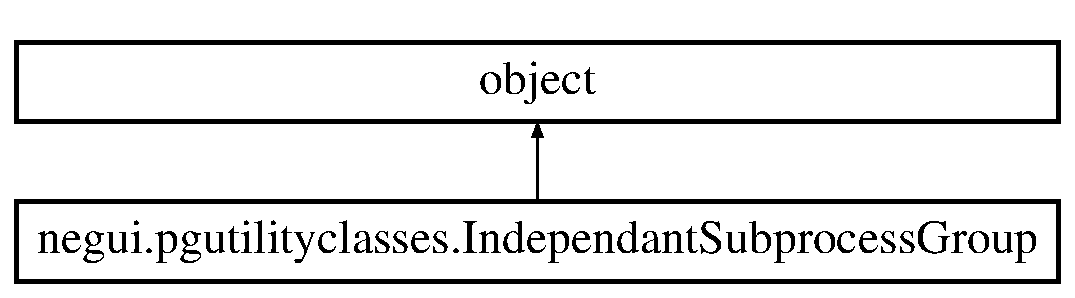
\includegraphics[height=2.000000cm]{classnegui_1_1pgutilityclasses_1_1IndependantSubprocessGroup}
\end{center}
\end{figure}
\subsection*{Public Member Functions}
\begin{DoxyCompactItemize}
\item 
def {\bfseries \+\_\+\+\_\+init\+\_\+\+\_\+} (self, lo\+\_\+subprocesses=\mbox{[}$\,$\mbox{]})\hypertarget{classnegui_1_1pgutilityclasses_1_1IndependantSubprocessGroup_ab847e4373b27ae8580a3036c6b91ee01}{}\label{classnegui_1_1pgutilityclasses_1_1IndependantSubprocessGroup_ab847e4373b27ae8580a3036c6b91ee01}

\item 
def {\bfseries add\+Subprocess} (self, o\+\_\+subprocess)\hypertarget{classnegui_1_1pgutilityclasses_1_1IndependantSubprocessGroup_afae1c628e1a6e7e719148864aeb9fb44}{}\label{classnegui_1_1pgutilityclasses_1_1IndependantSubprocessGroup_afae1c628e1a6e7e719148864aeb9fb44}

\item 
def {\bfseries get\+Total\+Alive} (self)\hypertarget{classnegui_1_1pgutilityclasses_1_1IndependantSubprocessGroup_ae0b95298715c71ad27fbb50a5c96cdc9}{}\label{classnegui_1_1pgutilityclasses_1_1IndependantSubprocessGroup_ae0b95298715c71ad27fbb50a5c96cdc9}

\item 
def {\bfseries terminate\+All\+Subprocesses} (self)\hypertarget{classnegui_1_1pgutilityclasses_1_1IndependantSubprocessGroup_a9a9608d560b556d3ea8635832ca7bf87}{}\label{classnegui_1_1pgutilityclasses_1_1IndependantSubprocessGroup_a9a9608d560b556d3ea8635832ca7bf87}

\end{DoxyCompactItemize}


\subsection{Detailed Description}
\begin{DoxyVerb}Minimal Revision of class independantProcessGroup   
to operate on python subprocess.Popen proccesses.

The main changes include use of kill() instead of 
terminate in def terminateAllSubprocesses() and
use poll() (is None) instead of is_alive() to get
a count of living processes
\end{DoxyVerb}
 

Definition at line 77 of file pgutilityclasses.\+py.



The documentation for this class was generated from the following file\+:\begin{DoxyCompactItemize}
\item 
pgutilityclasses.\+py\end{DoxyCompactItemize}

\hypertarget{classnegui_1_1pgkeycategoricalvalueframe_1_1KeyCategoricalValueFrame}{}\section{negui.\+pgkeycategoricalvalueframe.\+Key\+Categorical\+Value\+Frame Class Reference}
\label{classnegui_1_1pgkeycategoricalvalueframe_1_1KeyCategoricalValueFrame}\index{negui.\+pgkeycategoricalvalueframe.\+Key\+Categorical\+Value\+Frame@{negui.\+pgkeycategoricalvalueframe.\+Key\+Categorical\+Value\+Frame}}
Inheritance diagram for negui.\+pgkeycategoricalvalueframe.\+Key\+Categorical\+Value\+Frame\+:\begin{figure}[H]
\begin{center}
\leavevmode
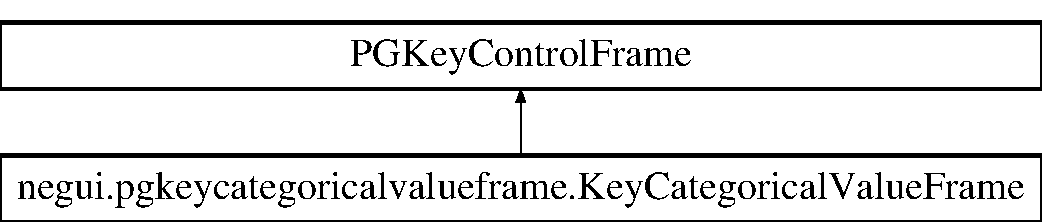
\includegraphics[height=2.000000cm]{classnegui_1_1pgkeycategoricalvalueframe_1_1KeyCategoricalValueFrame}
\end{center}
\end{figure}
\subsection*{Public Member Functions}
\begin{DoxyCompactItemize}
\item 
def \hyperlink{classnegui_1_1pgkeycategoricalvalueframe_1_1KeyCategoricalValueFrame_a2c9fb8441f73917f0a6f9af179c436ef}{\+\_\+\+\_\+init\+\_\+\+\_\+} (self, s\+\_\+name, lq\+\_\+modes, i\+\_\+default\+\_\+mode\+\_\+number, o\+\_\+value\+\_\+type=None, o\+\_\+master=None, s\+\_\+associated\+\_\+attribute=None, o\+\_\+associated\+\_\+attribute\+\_\+object=None, def\+\_\+on\+\_\+button\+\_\+change=None, i\+\_\+labelwidth=15, b\+\_\+is\+\_\+enabled=True, s\+\_\+label\+\_\+justify=\textquotesingle{}right\textquotesingle{}, s\+\_\+buttons\+\_\+justify=\textquotesingle{}right\textquotesingle{}, s\+\_\+label\+\_\+name=None, b\+\_\+buttons\+\_\+in\+\_\+a\+\_\+row=False, b\+\_\+force\+\_\+disable=False, s\+\_\+tooltip=\char`\"{}\char`\"{})
\item 
def \hyperlink{classnegui_1_1pgkeycategoricalvalueframe_1_1KeyCategoricalValueFrame_aff5c9286de1063277913c3274657f0bc}{set\+State\+Controls} (self, s\+\_\+state)
\item 
def {\bfseries get\+Control\+States} (self)\hypertarget{classnegui_1_1pgkeycategoricalvalueframe_1_1KeyCategoricalValueFrame_ac460db19a4cab594e44e35ec9dd7f64f}{}\label{classnegui_1_1pgkeycategoricalvalueframe_1_1KeyCategoricalValueFrame_ac460db19a4cab594e44e35ec9dd7f64f}

\item 
def {\bfseries is\+\_\+enabled} (self)\hypertarget{classnegui_1_1pgkeycategoricalvalueframe_1_1KeyCategoricalValueFrame_a89d7f62a48033e2bf1401795fc69ebc1}{}\label{classnegui_1_1pgkeycategoricalvalueframe_1_1KeyCategoricalValueFrame_a89d7f62a48033e2bf1401795fc69ebc1}

\item 
def {\bfseries force\+\_\+disable} (self)\hypertarget{classnegui_1_1pgkeycategoricalvalueframe_1_1KeyCategoricalValueFrame_a55d748475399ee7556e2eae72db69c38}{}\label{classnegui_1_1pgkeycategoricalvalueframe_1_1KeyCategoricalValueFrame_a55d748475399ee7556e2eae72db69c38}

\item 
def {\bfseries val} (self)\hypertarget{classnegui_1_1pgkeycategoricalvalueframe_1_1KeyCategoricalValueFrame_aa4259a98893ee65f1ec8e0f2f6bf3288}{}\label{classnegui_1_1pgkeycategoricalvalueframe_1_1KeyCategoricalValueFrame_aa4259a98893ee65f1ec8e0f2f6bf3288}

\item 
def {\bfseries val} (self)\hypertarget{classnegui_1_1pgkeycategoricalvalueframe_1_1KeyCategoricalValueFrame_aa4259a98893ee65f1ec8e0f2f6bf3288}{}\label{classnegui_1_1pgkeycategoricalvalueframe_1_1KeyCategoricalValueFrame_aa4259a98893ee65f1ec8e0f2f6bf3288}

\end{DoxyCompactItemize}
\subsection*{Public Attributes}
\begin{DoxyCompactItemize}
\item 
{\bfseries label}\hypertarget{classnegui_1_1pgkeycategoricalvalueframe_1_1KeyCategoricalValueFrame_a705820b0a648b0df569e23677d2e0e10}{}\label{classnegui_1_1pgkeycategoricalvalueframe_1_1KeyCategoricalValueFrame_a705820b0a648b0df569e23677d2e0e10}

\end{DoxyCompactItemize}


\subsection{Detailed Description}
\begin{DoxyVerb}Description

Revised KeyValueFrame
substituting a Radiobutton widget
for the entry box used in KeyValFrame\end{DoxyVerb}
 

Definition at line 30 of file pgkeycategoricalvalueframe.\+py.



\subsection{Constructor \& Destructor Documentation}
\index{negui\+::pgkeycategoricalvalueframe\+::\+Key\+Categorical\+Value\+Frame@{negui\+::pgkeycategoricalvalueframe\+::\+Key\+Categorical\+Value\+Frame}!\+\_\+\+\_\+init\+\_\+\+\_\+@{\+\_\+\+\_\+init\+\_\+\+\_\+}}
\index{\+\_\+\+\_\+init\+\_\+\+\_\+@{\+\_\+\+\_\+init\+\_\+\+\_\+}!negui\+::pgkeycategoricalvalueframe\+::\+Key\+Categorical\+Value\+Frame@{negui\+::pgkeycategoricalvalueframe\+::\+Key\+Categorical\+Value\+Frame}}
\subsubsection[{\texorpdfstring{\+\_\+\+\_\+init\+\_\+\+\_\+(self, s\+\_\+name, lq\+\_\+modes, i\+\_\+default\+\_\+mode\+\_\+number, o\+\_\+value\+\_\+type=\+None, o\+\_\+master=\+None, s\+\_\+associated\+\_\+attribute=\+None, o\+\_\+associated\+\_\+attribute\+\_\+object=\+None, def\+\_\+on\+\_\+button\+\_\+change=\+None, i\+\_\+labelwidth=15, b\+\_\+is\+\_\+enabled=\+True, s\+\_\+label\+\_\+justify=\textquotesingle{}right\textquotesingle{}, s\+\_\+buttons\+\_\+justify=\textquotesingle{}right\textquotesingle{}, s\+\_\+label\+\_\+name=\+None, b\+\_\+buttons\+\_\+in\+\_\+a\+\_\+row=\+False, b\+\_\+force\+\_\+disable=\+False, s\+\_\+tooltip="""")}{__init__(self, s_name, lq_modes, i_default_mode_number, o_value_type=None, o_master=None, s_associated_attribute=None, o_associated_attribute_object=None, def_on_button_change=None, i_labelwidth=15, b_is_enabled=True, s_label_justify='right', s_buttons_justify='right', s_label_name=None, b_buttons_in_a_row=False, b_force_disable=False, s_tooltip="")}}]{\setlength{\rightskip}{0pt plus 5cm}def negui.\+pgkeycategoricalvalueframe.\+Key\+Categorical\+Value\+Frame.\+\_\+\+\_\+init\+\_\+\+\_\+ (
\begin{DoxyParamCaption}
\item[{}]{self, }
\item[{}]{s\+\_\+name, }
\item[{}]{lq\+\_\+modes, }
\item[{}]{i\+\_\+default\+\_\+mode\+\_\+number, }
\item[{}]{o\+\_\+value\+\_\+type = {\ttfamily None}, }
\item[{}]{o\+\_\+master = {\ttfamily None}, }
\item[{}]{s\+\_\+associated\+\_\+attribute = {\ttfamily None}, }
\item[{}]{o\+\_\+associated\+\_\+attribute\+\_\+object = {\ttfamily None}, }
\item[{}]{def\+\_\+on\+\_\+button\+\_\+change = {\ttfamily None}, }
\item[{}]{i\+\_\+labelwidth = {\ttfamily 15}, }
\item[{}]{b\+\_\+is\+\_\+enabled = {\ttfamily True}, }
\item[{}]{s\+\_\+label\+\_\+justify = {\ttfamily \textquotesingle{}right\textquotesingle{}}, }
\item[{}]{s\+\_\+buttons\+\_\+justify = {\ttfamily \textquotesingle{}right\textquotesingle{}}, }
\item[{}]{s\+\_\+label\+\_\+name = {\ttfamily None}, }
\item[{}]{b\+\_\+buttons\+\_\+in\+\_\+a\+\_\+row = {\ttfamily False}, }
\item[{}]{b\+\_\+force\+\_\+disable = {\ttfamily False}, }
\item[{}]{s\+\_\+tooltip = {\ttfamily \char`\"{}\char`\"{}}}
\end{DoxyParamCaption}
)}\hypertarget{classnegui_1_1pgkeycategoricalvalueframe_1_1KeyCategoricalValueFrame_a2c9fb8441f73917f0a6f9af179c436ef}{}\label{classnegui_1_1pgkeycategoricalvalueframe_1_1KeyCategoricalValueFrame_a2c9fb8441f73917f0a6f9af179c436ef}
\begin{DoxyVerb}Param lq_modes, list of sequences, each a pair
    giving the mode label text, and its associated value
    assigned when it is the selected radio button
Param i_default_mode_number gives the ith (one-indexed)
    item in modes, that is to be the active button,
    and that gives the default value
Param o_value_type gives the python type for the values
    given in lq_modes value items.  Currently implemented
    for bool, int, float, and string.
Param o_master is the parent Tkinter object.
Param s_associated_attribute is the name of 
    attribute instance that can be accessed
    using "getattr", and that will be
    updated when the value is updated.
Param o_associated_attribute_object is the object whose attribute
    is to be unpdated when the value is updated.  If
    s_associated_attribute is not None, and this parameter
    is None, the attribute is presumed to be
    owned by the o_master object.
Param def_on_button_change, if not None, execute the def
    after updating both the value and the attribute (if any).
    This def is to have no passed params.
Param i_labelwidth gives the width the the Label widget.
Param s_label_justify gives Label widget "justify" value.
Param s_buttons_justify gives Radiobutten Widget text "justify" value.
currently not implemented (ttk radio button widgets are not
settable for justify and foreground, without using a syle map).
Param s_label_name, if not None, replaces s_name as the text for the label.
Param b_buttons_in_a_row, if False (default) all buttons are in a single column, if True,
then all buttons side by side in a single row
Param b_force_disable, if True, will override the b_is_enabled value and disable all entry 
      boxes
\end{DoxyVerb}
 

Definition at line 56 of file pgkeycategoricalvalueframe.\+py.


\begin{DoxyCode}
56             s\_tooltip = \textcolor{stringliteral}{""} ):
57 
58         \textcolor{stringliteral}{"""}
59 \textcolor{stringliteral}{        Param lq\_modes, list of sequences, each a pair}
60 \textcolor{stringliteral}{            giving the mode label text, and its associated value}
61 \textcolor{stringliteral}{            assigned when it is the selected radio button}
62 \textcolor{stringliteral}{        Param i\_default\_mode\_number gives the ith (one-indexed)}
63 \textcolor{stringliteral}{            item in modes, that is to be the active button,}
64 \textcolor{stringliteral}{            and that gives the default value}
65 \textcolor{stringliteral}{        Param o\_value\_type gives the python type for the values}
66 \textcolor{stringliteral}{            given in lq\_modes value items.  Currently implemented}
67 \textcolor{stringliteral}{            for bool, int, float, and string.}
68 \textcolor{stringliteral}{        Param o\_master is the parent Tkinter object.}
69 \textcolor{stringliteral}{                Param s\_associated\_attribute is the name of }
70 \textcolor{stringliteral}{            attribute instance that can be accessed}
71 \textcolor{stringliteral}{            using "getattr", and that will be}
72 \textcolor{stringliteral}{            updated when the value is updated.}
73 \textcolor{stringliteral}{        Param o\_associated\_attribute\_object is the object whose attribute}
74 \textcolor{stringliteral}{            is to be unpdated when the value is updated.  If}
75 \textcolor{stringliteral}{            s\_associated\_attribute is not None, and this parameter}
76 \textcolor{stringliteral}{            is None, the attribute is presumed to be}
77 \textcolor{stringliteral}{            owned by the o\_master object.}
78 \textcolor{stringliteral}{        Param def\_on\_button\_change, if not None, execute the def}
79 \textcolor{stringliteral}{            after updating both the value and the attribute (if any).}
80 \textcolor{stringliteral}{            This def is to have no passed params.}
81 \textcolor{stringliteral}{        Param i\_labelwidth gives the width the the Label widget.}
82 \textcolor{stringliteral}{        Param s\_label\_justify gives Label widget "justify" value.}
83 \textcolor{stringliteral}{        Param s\_buttons\_justify gives Radiobutten Widget text "justify" value.}
84 \textcolor{stringliteral}{                currently not implemented (ttk radio button widgets are not}
85 \textcolor{stringliteral}{                settable for justify and foreground, without using a syle map).}
86 \textcolor{stringliteral}{        Param s\_label\_name, if not None, replaces s\_name as the text for the label.}
87 \textcolor{stringliteral}{        Param b\_buttons\_in\_a\_row, if False (default) all buttons are in a single column, if True,}
88 \textcolor{stringliteral}{                then all buttons side by side in a single row}
89 \textcolor{stringliteral}{        Param b\_force\_disable, if True, will override the b\_is\_enabled value and disable all entry }
90 \textcolor{stringliteral}{              boxes}
91 \textcolor{stringliteral}{        """}
92 
93         PGKeyControlFrame.\_\_init\_\_( self, o\_master, name=s\_name.lower() )
94 
95         self.\hyperlink{classnegui_1_1pgkeycategoricalvalueframe_1_1KeyCategoricalValueFrame_a37392e2348ae8798c3719ea521e7b187}{\_\_master}=o\_master
96         self.\hyperlink{classnegui_1_1pgkeycategoricalvalueframe_1_1KeyCategoricalValueFrame_aa2f3ec53994ee9d5e28cbf91e2bb8f6b}{\_\_value}=\textcolor{keywordtype}{None}
97         self.\hyperlink{classnegui_1_1pgkeycategoricalvalueframe_1_1KeyCategoricalValueFrame_afd4c9d1f7d637f99544df949d6cd713a}{\_\_default\_mode\_number}=i\_default\_mode\_number
98         self.\hyperlink{classnegui_1_1pgkeycategoricalvalueframe_1_1KeyCategoricalValueFrame_ab0c13b2b8e7db616aa16eb76d984f96c}{\_\_modes}=lq\_modes
99         self.\hyperlink{classnegui_1_1pgkeycategoricalvalueframe_1_1KeyCategoricalValueFrame_a902632de5675cd128bd4c6665ff7c997}{\_\_name}=s\_name
100         self.\hyperlink{classnegui_1_1pgkeycategoricalvalueframe_1_1KeyCategoricalValueFrame_a252538703840fb6070a820cfee3f75d2}{\_\_lablewidth}=i\_labelwidth
101         self.\hyperlink{classnegui_1_1pgkeycategoricalvalueframe_1_1KeyCategoricalValueFrame_a4c5afbabd0f905b497ac5368d8f9e02c}{\_\_labeljustify}=s\_label\_justify
102         self.\hyperlink{classnegui_1_1pgkeycategoricalvalueframe_1_1KeyCategoricalValueFrame_af3cd0e08362f041b7ddca1e1da4cfa92}{\_\_buttons\_justify}=s\_buttons\_justify
103         self.\hyperlink{classnegui_1_1pgkeycategoricalvalueframe_1_1KeyCategoricalValueFrame_aa802dcfac6205afe32ed2c9116815fa8}{\_\_isenabled}=b\_is\_enabled
104         self.\hyperlink{classnegui_1_1pgkeycategoricalvalueframe_1_1KeyCategoricalValueFrame_aa618957880cc556fdba51cb83b3d3a7f}{\_\_associated\_attribute}=s\_associated\_attribute
105         self.\hyperlink{classnegui_1_1pgkeycategoricalvalueframe_1_1KeyCategoricalValueFrame_a299f08e826dbb833003d57a8914956b8}{\_\_associated\_attribute\_object}=o\_associated\_attribute\_object
106         self.\hyperlink{classnegui_1_1pgkeycategoricalvalueframe_1_1KeyCategoricalValueFrame_a3bbc63953105d66f89f2c556ca6aa7e7}{\_\_def\_on\_button\_change}=def\_on\_button\_change
107         self.\hyperlink{classnegui_1_1pgkeycategoricalvalueframe_1_1KeyCategoricalValueFrame_a857b3e800db184ac5b9bfdc8569bcf05}{\_\_put\_buttons\_in\_row}=b\_buttons\_in\_a\_row
108         self.\hyperlink{classnegui_1_1pgkeycategoricalvalueframe_1_1KeyCategoricalValueFrame_a05d5f3c927aa1504d765821b403d2401}{\_\_current\_button\_value}=self.
      \hyperlink{classnegui_1_1pgkeycategoricalvalueframe_1_1KeyCategoricalValueFrame_ac5f25071d919a515479c6535fda1cdf7}{\_\_init\_current\_button\_val}( o\_value\_type )
109         self.\hyperlink{classnegui_1_1pgkeycategoricalvalueframe_1_1KeyCategoricalValueFrame_af8854649c62924012d90cfdab7714883}{\_\_label\_name}=self.\hyperlink{classnegui_1_1pgkeycategoricalvalueframe_1_1KeyCategoricalValueFrame_a902632de5675cd128bd4c6665ff7c997}{\_\_name} \textcolor{keywordflow}{if} s\_label\_name \textcolor{keywordflow}{is} \textcolor{keywordtype}{None} \textcolor{keywordflow}{else} s\_label\_name
110         self.\hyperlink{classnegui_1_1pgkeycategoricalvalueframe_1_1KeyCategoricalValueFrame_adcb54d6b7ebcbfa69ec2142e0fbc9bd5}{\_\_force\_disable}=b\_force\_disable
111         self.\hyperlink{classnegui_1_1pgkeycategoricalvalueframe_1_1KeyCategoricalValueFrame_abb96b16610f49b28b4541339091811c5}{\_\_tooltip}=self.\hyperlink{classnegui_1_1pgkeycategoricalvalueframe_1_1KeyCategoricalValueFrame_af8854649c62924012d90cfdab7714883}{\_\_label\_name} \textcolor{keywordflow}{if} s\_tooltip == \textcolor{stringliteral}{""} \textcolor{keywordflow}{else} s\_tooltip
112         self.\hyperlink{classnegui_1_1pgkeycategoricalvalueframe_1_1KeyCategoricalValueFrame_a7b8e397259ee2874be3ab13dd67c5d61}{\_\_subframe}=\textcolor{keywordtype}{None}
113 
114         \textcolor{comment}{#To maintain a reference to the Radiobutton objects,}
115         \textcolor{comment}{#this will be appended-to as they are created:}
116         self.\hyperlink{classnegui_1_1pgkeycategoricalvalueframe_1_1KeyCategoricalValueFrame_a0742fecf915163b9068ff58b6d846ef1}{\_\_radio\_buttons}=[]
117         self.\hyperlink{classnegui_1_1pgkeycategoricalvalueframe_1_1KeyCategoricalValueFrame_a30e70d9767675f265df2122a5d8a3b9a}{\_\_setup}()
\end{DoxyCode}


\subsection{Member Function Documentation}
\index{negui\+::pgkeycategoricalvalueframe\+::\+Key\+Categorical\+Value\+Frame@{negui\+::pgkeycategoricalvalueframe\+::\+Key\+Categorical\+Value\+Frame}!set\+State\+Controls@{set\+State\+Controls}}
\index{set\+State\+Controls@{set\+State\+Controls}!negui\+::pgkeycategoricalvalueframe\+::\+Key\+Categorical\+Value\+Frame@{negui\+::pgkeycategoricalvalueframe\+::\+Key\+Categorical\+Value\+Frame}}
\subsubsection[{\texorpdfstring{set\+State\+Controls(self, s\+\_\+state)}{setStateControls(self, s_state)}}]{\setlength{\rightskip}{0pt plus 5cm}def negui.\+pgkeycategoricalvalueframe.\+Key\+Categorical\+Value\+Frame.\+set\+State\+Controls (
\begin{DoxyParamCaption}
\item[{}]{self, }
\item[{}]{s\+\_\+state}
\end{DoxyParamCaption}
)}\hypertarget{classnegui_1_1pgkeycategoricalvalueframe_1_1KeyCategoricalValueFrame_aff5c9286de1063277913c3274657f0bc}{}\label{classnegui_1_1pgkeycategoricalvalueframe_1_1KeyCategoricalValueFrame_aff5c9286de1063277913c3274657f0bc}
\begin{DoxyVerb}Set the state of all this objects
radio buttons.
\end{DoxyVerb}
 

Definition at line 297 of file pgkeycategoricalvalueframe.\+py.


\begin{DoxyCode}
297     \textcolor{keyword}{def }\hyperlink{classnegui_1_1pgkeycategoricalvalueframe_1_1KeyCategoricalValueFrame_aff5c9286de1063277913c3274657f0bc}{setStateControls}( self, s\_state ):
298         \textcolor{stringliteral}{'''}
299 \textcolor{stringliteral}{        Set the state of all this objects}
300 \textcolor{stringliteral}{        radio buttons.}
301 \textcolor{stringliteral}{        '''}
302         \textcolor{keywordflow}{for} o\_radio\_button \textcolor{keywordflow}{in} self.\hyperlink{classnegui_1_1pgkeycategoricalvalueframe_1_1KeyCategoricalValueFrame_a0742fecf915163b9068ff58b6d846ef1}{\_\_radio\_buttons}:
303             o\_radio\_button.configure( state=s\_state )
304         \textcolor{comment}{#end for each entry box}
305 
306         \textcolor{keywordflow}{return}
\end{DoxyCode}


The documentation for this class was generated from the following file\+:\begin{DoxyCompactItemize}
\item 
pgkeycategoricalvalueframe.\+py\end{DoxyCompactItemize}

\hypertarget{classnegui_1_1pgkeycheckboxvalueframe_1_1KeyCheckboxValueFrame}{}\section{negui.\+pgkeycheckboxvalueframe.\+Key\+Checkbox\+Value\+Frame Class Reference}
\label{classnegui_1_1pgkeycheckboxvalueframe_1_1KeyCheckboxValueFrame}\index{negui.\+pgkeycheckboxvalueframe.\+Key\+Checkbox\+Value\+Frame@{negui.\+pgkeycheckboxvalueframe.\+Key\+Checkbox\+Value\+Frame}}
Inheritance diagram for negui.\+pgkeycheckboxvalueframe.\+Key\+Checkbox\+Value\+Frame\+:\begin{figure}[H]
\begin{center}
\leavevmode
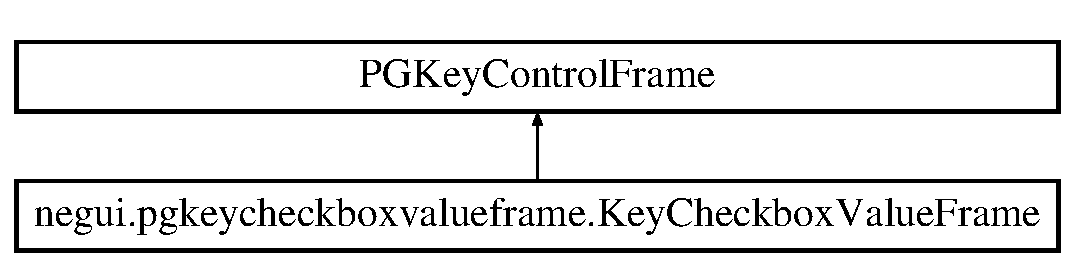
\includegraphics[height=2.000000cm]{classnegui_1_1pgkeycheckboxvalueframe_1_1KeyCheckboxValueFrame}
\end{center}
\end{figure}
\subsection*{Public Member Functions}
\begin{DoxyCompactItemize}
\item 
def \hyperlink{classnegui_1_1pgkeycheckboxvalueframe_1_1KeyCheckboxValueFrame_a67edc291a493061206f1bf93ced6137e}{\+\_\+\+\_\+init\+\_\+\+\_\+} (self, s\+\_\+name, v\+\_\+value=True, o\+\_\+master=None, s\+\_\+associated\+\_\+attribute=None, o\+\_\+associated\+\_\+attribute\+\_\+object=None, def\+\_\+on\+\_\+button\+\_\+change=None, i\+\_\+labelwidth=15, b\+\_\+is\+\_\+enabled=True, s\+\_\+label\+\_\+justify=\textquotesingle{}right\textquotesingle{}, s\+\_\+label\+\_\+name=None, b\+\_\+force\+\_\+disable=False, s\+\_\+tooltip=\char`\"{}\char`\"{})
\item 
def \hyperlink{classnegui_1_1pgkeycheckboxvalueframe_1_1KeyCheckboxValueFrame_a40238b6852e83078ef986454da75aaab}{set\+State\+Controls} (self, s\+\_\+state)
\item 
def {\bfseries get\+Control\+States} (self)\hypertarget{classnegui_1_1pgkeycheckboxvalueframe_1_1KeyCheckboxValueFrame_a7e95370cbe2405a45eb03fbcd6538c45}{}\label{classnegui_1_1pgkeycheckboxvalueframe_1_1KeyCheckboxValueFrame_a7e95370cbe2405a45eb03fbcd6538c45}

\item 
def {\bfseries is\+\_\+enabled} (self)\hypertarget{classnegui_1_1pgkeycheckboxvalueframe_1_1KeyCheckboxValueFrame_ae6d65342f8ba05ad56034af485df08d0}{}\label{classnegui_1_1pgkeycheckboxvalueframe_1_1KeyCheckboxValueFrame_ae6d65342f8ba05ad56034af485df08d0}

\item 
def {\bfseries force\+\_\+disable} (self)\hypertarget{classnegui_1_1pgkeycheckboxvalueframe_1_1KeyCheckboxValueFrame_a9d6c98c493c5006d01c681bf5afa773d}{}\label{classnegui_1_1pgkeycheckboxvalueframe_1_1KeyCheckboxValueFrame_a9d6c98c493c5006d01c681bf5afa773d}

\item 
def {\bfseries val} (self)\hypertarget{classnegui_1_1pgkeycheckboxvalueframe_1_1KeyCheckboxValueFrame_ab33583afb366b88cb973443c2528c1cb}{}\label{classnegui_1_1pgkeycheckboxvalueframe_1_1KeyCheckboxValueFrame_ab33583afb366b88cb973443c2528c1cb}

\item 
def {\bfseries val} (self)\hypertarget{classnegui_1_1pgkeycheckboxvalueframe_1_1KeyCheckboxValueFrame_ab33583afb366b88cb973443c2528c1cb}{}\label{classnegui_1_1pgkeycheckboxvalueframe_1_1KeyCheckboxValueFrame_ab33583afb366b88cb973443c2528c1cb}

\end{DoxyCompactItemize}
\subsection*{Public Attributes}
\begin{DoxyCompactItemize}
\item 
{\bfseries label}\hypertarget{classnegui_1_1pgkeycheckboxvalueframe_1_1KeyCheckboxValueFrame_a172178389b7c214455b25fd51ae68a78}{}\label{classnegui_1_1pgkeycheckboxvalueframe_1_1KeyCheckboxValueFrame_a172178389b7c214455b25fd51ae68a78}

\end{DoxyCompactItemize}


\subsection{Detailed Description}
\begin{DoxyVerb}Description

Revised KeyValueFrame
substituting a Checkbutton widget
for the entry box used in KeyValFrame\end{DoxyVerb}
 

Definition at line 30 of file pgkeycheckboxvalueframe.\+py.



\subsection{Constructor \& Destructor Documentation}
\index{negui\+::pgkeycheckboxvalueframe\+::\+Key\+Checkbox\+Value\+Frame@{negui\+::pgkeycheckboxvalueframe\+::\+Key\+Checkbox\+Value\+Frame}!\+\_\+\+\_\+init\+\_\+\+\_\+@{\+\_\+\+\_\+init\+\_\+\+\_\+}}
\index{\+\_\+\+\_\+init\+\_\+\+\_\+@{\+\_\+\+\_\+init\+\_\+\+\_\+}!negui\+::pgkeycheckboxvalueframe\+::\+Key\+Checkbox\+Value\+Frame@{negui\+::pgkeycheckboxvalueframe\+::\+Key\+Checkbox\+Value\+Frame}}
\subsubsection[{\texorpdfstring{\+\_\+\+\_\+init\+\_\+\+\_\+(self, s\+\_\+name, v\+\_\+value=\+True, o\+\_\+master=\+None, s\+\_\+associated\+\_\+attribute=\+None, o\+\_\+associated\+\_\+attribute\+\_\+object=\+None, def\+\_\+on\+\_\+button\+\_\+change=\+None, i\+\_\+labelwidth=15, b\+\_\+is\+\_\+enabled=\+True, s\+\_\+label\+\_\+justify=\textquotesingle{}right\textquotesingle{}, s\+\_\+label\+\_\+name=\+None, b\+\_\+force\+\_\+disable=\+False, s\+\_\+tooltip="""")}{__init__(self, s_name, v_value=True, o_master=None, s_associated_attribute=None, o_associated_attribute_object=None, def_on_button_change=None, i_labelwidth=15, b_is_enabled=True, s_label_justify='right', s_label_name=None, b_force_disable=False, s_tooltip="")}}]{\setlength{\rightskip}{0pt plus 5cm}def negui.\+pgkeycheckboxvalueframe.\+Key\+Checkbox\+Value\+Frame.\+\_\+\+\_\+init\+\_\+\+\_\+ (
\begin{DoxyParamCaption}
\item[{}]{self, }
\item[{}]{s\+\_\+name, }
\item[{}]{v\+\_\+value = {\ttfamily True}, }
\item[{}]{o\+\_\+master = {\ttfamily None}, }
\item[{}]{s\+\_\+associated\+\_\+attribute = {\ttfamily None}, }
\item[{}]{o\+\_\+associated\+\_\+attribute\+\_\+object = {\ttfamily None}, }
\item[{}]{def\+\_\+on\+\_\+button\+\_\+change = {\ttfamily None}, }
\item[{}]{i\+\_\+labelwidth = {\ttfamily 15}, }
\item[{}]{b\+\_\+is\+\_\+enabled = {\ttfamily True}, }
\item[{}]{s\+\_\+label\+\_\+justify = {\ttfamily \textquotesingle{}right\textquotesingle{}}, }
\item[{}]{s\+\_\+label\+\_\+name = {\ttfamily None}, }
\item[{}]{b\+\_\+force\+\_\+disable = {\ttfamily False}, }
\item[{}]{s\+\_\+tooltip = {\ttfamily \char`\"{}\char`\"{}}}
\end{DoxyParamCaption}
)}\hypertarget{classnegui_1_1pgkeycheckboxvalueframe_1_1KeyCheckboxValueFrame_a67edc291a493061206f1bf93ced6137e}{}\label{classnegui_1_1pgkeycheckboxvalueframe_1_1KeyCheckboxValueFrame_a67edc291a493061206f1bf93ced6137e}
\begin{DoxyVerb}Param lq_modes, list of sequences, each a pair
    giving the mode label text, and its associated value
    assigned when it is the selected radio button
Param o_master is the parent Tkinter object.
Param s_associated_attribute is the name of 
    attribute instance that can be accessed
    using "getattr", and that will be
    updated when the value is updated.
Param o_associated_attribute_object is the object whose attribute
    is to be unpdated when the value is updated.  If
    s_associated_attribute is not None, and this parameter
    is None, the attribute is presumed to be
    owned by the o_master object.
Param def_on_button_change, if not None, execute the def
    after updating both the value and the attribute (if any).
    This def is to have no passed params.
Param i_labelwidth gives the width the the Label widget.
Param s_label_justify gives Label widget "justify" value.
Param s_label_name, if not None, replaces s_name as the text for the label.
Param b_force_disable, if True, will override the b_is_enabled value and disable all entry 
      boxes
\end{DoxyVerb}
 

Definition at line 52 of file pgkeycheckboxvalueframe.\+py.


\begin{DoxyCode}
52             s\_tooltip = \textcolor{stringliteral}{""} ):
53 
54         \textcolor{stringliteral}{"""}
55 \textcolor{stringliteral}{        Param lq\_modes, list of sequences, each a pair}
56 \textcolor{stringliteral}{            giving the mode label text, and its associated value}
57 \textcolor{stringliteral}{            assigned when it is the selected radio button}
58 \textcolor{stringliteral}{        Param o\_master is the parent Tkinter object.}
59 \textcolor{stringliteral}{                Param s\_associated\_attribute is the name of }
60 \textcolor{stringliteral}{            attribute instance that can be accessed}
61 \textcolor{stringliteral}{            using "getattr", and that will be}
62 \textcolor{stringliteral}{            updated when the value is updated.}
63 \textcolor{stringliteral}{        Param o\_associated\_attribute\_object is the object whose attribute}
64 \textcolor{stringliteral}{            is to be unpdated when the value is updated.  If}
65 \textcolor{stringliteral}{            s\_associated\_attribute is not None, and this parameter}
66 \textcolor{stringliteral}{            is None, the attribute is presumed to be}
67 \textcolor{stringliteral}{            owned by the o\_master object.}
68 \textcolor{stringliteral}{        Param def\_on\_button\_change, if not None, execute the def}
69 \textcolor{stringliteral}{            after updating both the value and the attribute (if any).}
70 \textcolor{stringliteral}{            This def is to have no passed params.}
71 \textcolor{stringliteral}{        Param i\_labelwidth gives the width the the Label widget.}
72 \textcolor{stringliteral}{        Param s\_label\_justify gives Label widget "justify" value.}
73 \textcolor{stringliteral}{        Param s\_label\_name, if not None, replaces s\_name as the text for the label.}
74 \textcolor{stringliteral}{        Param b\_force\_disable, if True, will override the b\_is\_enabled value and disable all entry }
75 \textcolor{stringliteral}{              boxes}
76 \textcolor{stringliteral}{        """}
77 
78         PGKeyControlFrame.\_\_init\_\_( self, o\_master, name=s\_name.lower() )
79 
80         self.\hyperlink{classnegui_1_1pgkeycheckboxvalueframe_1_1KeyCheckboxValueFrame_a90a6f743626f7dd0711dd3cc9f23fc05}{\_\_master}=o\_master
81         self.\hyperlink{classnegui_1_1pgkeycheckboxvalueframe_1_1KeyCheckboxValueFrame_a295bcfc16e29aec1d1c2b16b7c18ac94}{\_\_value}=v\_value
82         self.\hyperlink{classnegui_1_1pgkeycheckboxvalueframe_1_1KeyCheckboxValueFrame_a93336ce9b80c39f842e505b1b1be5873}{\_\_name}=s\_name
83         self.\hyperlink{classnegui_1_1pgkeycheckboxvalueframe_1_1KeyCheckboxValueFrame_a26a3c64b67eb07c20d7e8c7b4e21ef65}{\_\_lablewidth}=i\_labelwidth
84         self.\hyperlink{classnegui_1_1pgkeycheckboxvalueframe_1_1KeyCheckboxValueFrame_a815d815b46128a329784cee0f97622e8}{\_\_labeljustify}=s\_label\_justify
85         self.\hyperlink{classnegui_1_1pgkeycheckboxvalueframe_1_1KeyCheckboxValueFrame_a0558a97e5e8b8b03a5b232f960970af6}{\_\_isenabled}=b\_is\_enabled
86         self.\hyperlink{classnegui_1_1pgkeycheckboxvalueframe_1_1KeyCheckboxValueFrame_a8470f8886c61febe572b22fc327ddc4e}{\_\_associated\_attribute}=s\_associated\_attribute
87         self.\hyperlink{classnegui_1_1pgkeycheckboxvalueframe_1_1KeyCheckboxValueFrame_a08e3ca0981a04a1d6ea5a3353685a96e}{\_\_associated\_attribute\_object}=o\_associated\_attribute\_object
88         self.\hyperlink{classnegui_1_1pgkeycheckboxvalueframe_1_1KeyCheckboxValueFrame_aa4b047b5be71753a54a12d816286d730}{\_\_def\_on\_button\_change}=def\_on\_button\_change
89         self.\hyperlink{classnegui_1_1pgkeycheckboxvalueframe_1_1KeyCheckboxValueFrame_a7ccb95830ea7ba825f35c64149e61e0f}{\_\_label\_name}=self.\hyperlink{classnegui_1_1pgkeycheckboxvalueframe_1_1KeyCheckboxValueFrame_a93336ce9b80c39f842e505b1b1be5873}{\_\_name} \textcolor{keywordflow}{if} s\_label\_name \textcolor{keywordflow}{is} \textcolor{keywordtype}{None} \textcolor{keywordflow}{else} s\_label\_name
90         self.\hyperlink{classnegui_1_1pgkeycheckboxvalueframe_1_1KeyCheckboxValueFrame_a613ecc5454a56bbc974daddcd09e7d8d}{\_\_force\_disable}=b\_force\_disable
91         self.\hyperlink{classnegui_1_1pgkeycheckboxvalueframe_1_1KeyCheckboxValueFrame_a90e3ddc6c3b7bdb785fa873a1c330948}{\_\_tooltip}=self.\hyperlink{classnegui_1_1pgkeycheckboxvalueframe_1_1KeyCheckboxValueFrame_a7ccb95830ea7ba825f35c64149e61e0f}{\_\_label\_name} \textcolor{keywordflow}{if} s\_tooltip == \textcolor{stringliteral}{""} \textcolor{keywordflow}{else} s\_tooltip
92         self.\hyperlink{classnegui_1_1pgkeycheckboxvalueframe_1_1KeyCheckboxValueFrame_a33e2a1631b2a014561f79d968f42d5bd}{\_\_subframe}=\textcolor{keywordtype}{None}
93 
94         \textcolor{comment}{#To maintain a reference to the Checkbutton object,}
95         \textcolor{comment}{#this will be appended-to as they are created:}
96         self.\hyperlink{classnegui_1_1pgkeycheckboxvalueframe_1_1KeyCheckboxValueFrame_a23442af68e7d36eb839030eeef2674ab}{\_\_check\_button}=\textcolor{keywordtype}{None}
97 
98         self.\hyperlink{classnegui_1_1pgkeycheckboxvalueframe_1_1KeyCheckboxValueFrame_a48aaf9dfc2eebd016bfa4a4a69b9e28b}{\_\_current\_button\_value}=BooleanVar()
99         self.\_\_current\_button\_value.set( v\_value )
100         self.\hyperlink{classnegui_1_1pgkeycheckboxvalueframe_1_1KeyCheckboxValueFrame_a5870c368e38f7dc699ba568f659da4aa}{\_\_setup}()
101 
\end{DoxyCode}


\subsection{Member Function Documentation}
\index{negui\+::pgkeycheckboxvalueframe\+::\+Key\+Checkbox\+Value\+Frame@{negui\+::pgkeycheckboxvalueframe\+::\+Key\+Checkbox\+Value\+Frame}!set\+State\+Controls@{set\+State\+Controls}}
\index{set\+State\+Controls@{set\+State\+Controls}!negui\+::pgkeycheckboxvalueframe\+::\+Key\+Checkbox\+Value\+Frame@{negui\+::pgkeycheckboxvalueframe\+::\+Key\+Checkbox\+Value\+Frame}}
\subsubsection[{\texorpdfstring{set\+State\+Controls(self, s\+\_\+state)}{setStateControls(self, s_state)}}]{\setlength{\rightskip}{0pt plus 5cm}def negui.\+pgkeycheckboxvalueframe.\+Key\+Checkbox\+Value\+Frame.\+set\+State\+Controls (
\begin{DoxyParamCaption}
\item[{}]{self, }
\item[{}]{s\+\_\+state}
\end{DoxyParamCaption}
)}\hypertarget{classnegui_1_1pgkeycheckboxvalueframe_1_1KeyCheckboxValueFrame_a40238b6852e83078ef986454da75aaab}{}\label{classnegui_1_1pgkeycheckboxvalueframe_1_1KeyCheckboxValueFrame_a40238b6852e83078ef986454da75aaab}
\begin{DoxyVerb}Set the Checkbutton's state.
\end{DoxyVerb}
 

Definition at line 233 of file pgkeycheckboxvalueframe.\+py.


\begin{DoxyCode}
233     \textcolor{keyword}{def }\hyperlink{classnegui_1_1pgkeycheckboxvalueframe_1_1KeyCheckboxValueFrame_a40238b6852e83078ef986454da75aaab}{setStateControls}( self, s\_state ):
234         \textcolor{stringliteral}{'''}
235 \textcolor{stringliteral}{        Set the Checkbutton's state.}
236 \textcolor{stringliteral}{        '''}
237         self.\_\_check\_button.configure( state=s\_state )
238 
239         \textcolor{keywordflow}{return}
\end{DoxyCode}


The documentation for this class was generated from the following file\+:\begin{DoxyCompactItemize}
\item 
pgkeycheckboxvalueframe.\+py\end{DoxyCompactItemize}

\hypertarget{classnegui_1_1pgkeylistcomboframe_1_1KeyListComboFrame}{}\section{negui.\+pgkeylistcomboframe.\+Key\+List\+Combo\+Frame Class Reference}
\label{classnegui_1_1pgkeylistcomboframe_1_1KeyListComboFrame}\index{negui.\+pgkeylistcomboframe.\+Key\+List\+Combo\+Frame@{negui.\+pgkeylistcomboframe.\+Key\+List\+Combo\+Frame}}
Inheritance diagram for negui.\+pgkeylistcomboframe.\+Key\+List\+Combo\+Frame\+:\begin{figure}[H]
\begin{center}
\leavevmode
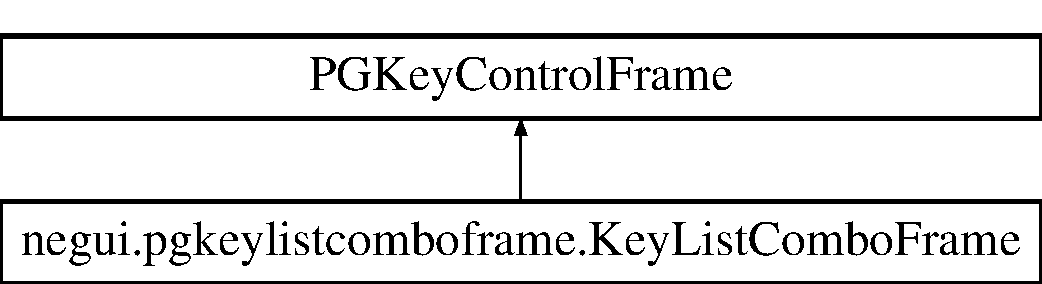
\includegraphics[height=2.000000cm]{classnegui_1_1pgkeylistcomboframe_1_1KeyListComboFrame}
\end{center}
\end{figure}
\subsection*{Public Member Functions}
\begin{DoxyCompactItemize}
\item 
def \hyperlink{classnegui_1_1pgkeylistcomboframe_1_1KeyListComboFrame_a5e92a43eef9e5a38c4337d185db637bd}{\+\_\+\+\_\+init\+\_\+\+\_\+} (self, s\+\_\+name, qs\+\_\+choices, i\+\_\+default\+\_\+choice\+\_\+number=1, o\+\_\+master=None, s\+\_\+associated\+\_\+attribute=None, o\+\_\+associated\+\_\+attribute\+\_\+object=None, def\+\_\+on\+\_\+new\+\_\+selection=None, i\+\_\+labelwidth=15, i\+\_\+cbox\+\_\+width=20, b\+\_\+is\+\_\+enabled=True, s\+\_\+label\+\_\+justify=\textquotesingle{}right\textquotesingle{}, s\+\_\+label\+\_\+name=None, b\+\_\+force\+\_\+disable=False, o\+\_\+validity\+\_\+tester=None, s\+\_\+state=\textquotesingle{}readonly\textquotesingle{}, s\+\_\+tooltip=\char`\"{}\char`\"{})
\item 
def \hyperlink{classnegui_1_1pgkeylistcomboframe_1_1KeyListComboFrame_a2b670cd4d4a38d03ae90df2786f076cb}{set\+State\+Controls} (self, s\+\_\+state)
\item 
def {\bfseries get\+Control\+States} (self)\hypertarget{classnegui_1_1pgkeylistcomboframe_1_1KeyListComboFrame_a2844d874ea9aac4c1ec0f8906099345f}{}\label{classnegui_1_1pgkeylistcomboframe_1_1KeyListComboFrame_a2844d874ea9aac4c1ec0f8906099345f}

\item 
def {\bfseries is\+\_\+enabled} (self)\hypertarget{classnegui_1_1pgkeylistcomboframe_1_1KeyListComboFrame_a796be506f3a271e058eeb375ef6c4713}{}\label{classnegui_1_1pgkeylistcomboframe_1_1KeyListComboFrame_a796be506f3a271e058eeb375ef6c4713}

\item 
def {\bfseries force\+\_\+disable} (self)\hypertarget{classnegui_1_1pgkeylistcomboframe_1_1KeyListComboFrame_af0a62d97038cca869e84b09679cca854}{}\label{classnegui_1_1pgkeylistcomboframe_1_1KeyListComboFrame_af0a62d97038cca869e84b09679cca854}

\item 
def {\bfseries val} (self)\hypertarget{classnegui_1_1pgkeylistcomboframe_1_1KeyListComboFrame_acca01b41da0563141822b38dee5e6efe}{}\label{classnegui_1_1pgkeylistcomboframe_1_1KeyListComboFrame_acca01b41da0563141822b38dee5e6efe}

\item 
def {\bfseries val} (self)\hypertarget{classnegui_1_1pgkeylistcomboframe_1_1KeyListComboFrame_acca01b41da0563141822b38dee5e6efe}{}\label{classnegui_1_1pgkeylistcomboframe_1_1KeyListComboFrame_acca01b41da0563141822b38dee5e6efe}

\end{DoxyCompactItemize}
\subsection*{Public Attributes}
\begin{DoxyCompactItemize}
\item 
{\bfseries label}\hypertarget{classnegui_1_1pgkeylistcomboframe_1_1KeyListComboFrame_a65085e88d0b71a00495a2e14299b3f65}{}\label{classnegui_1_1pgkeylistcomboframe_1_1KeyListComboFrame_a65085e88d0b71a00495a2e14299b3f65}

\end{DoxyCompactItemize}


\subsection{Detailed Description}
\begin{DoxyVerb}Description

Revised KeyValueFrame
substituting a combo box widget
for the entry box used in KeyValFrame.

The combobox updates the master
(or other parent subframe) with its
current selection.  Selections are always
strings.

This revised KeyValueFrame class was 
motivated by pgguineestimator.py interface
need to have a control by which users
select a genepop file sampling 
scheme. The the scheme name should then be a 
variable by which to offer sampling parameters
for the given sampling scheme, in I think 
a dynamically loaded subframe.
\end{DoxyVerb}
 

Definition at line 28 of file pgkeylistcomboframe.\+py.



\subsection{Constructor \& Destructor Documentation}
\index{negui\+::pgkeylistcomboframe\+::\+Key\+List\+Combo\+Frame@{negui\+::pgkeylistcomboframe\+::\+Key\+List\+Combo\+Frame}!\+\_\+\+\_\+init\+\_\+\+\_\+@{\+\_\+\+\_\+init\+\_\+\+\_\+}}
\index{\+\_\+\+\_\+init\+\_\+\+\_\+@{\+\_\+\+\_\+init\+\_\+\+\_\+}!negui\+::pgkeylistcomboframe\+::\+Key\+List\+Combo\+Frame@{negui\+::pgkeylistcomboframe\+::\+Key\+List\+Combo\+Frame}}
\subsubsection[{\texorpdfstring{\+\_\+\+\_\+init\+\_\+\+\_\+(self, s\+\_\+name, qs\+\_\+choices, i\+\_\+default\+\_\+choice\+\_\+number=1, o\+\_\+master=\+None, s\+\_\+associated\+\_\+attribute=\+None, o\+\_\+associated\+\_\+attribute\+\_\+object=\+None, def\+\_\+on\+\_\+new\+\_\+selection=\+None, i\+\_\+labelwidth=15, i\+\_\+cbox\+\_\+width=20, b\+\_\+is\+\_\+enabled=\+True, s\+\_\+label\+\_\+justify=\textquotesingle{}right\textquotesingle{}, s\+\_\+label\+\_\+name=\+None, b\+\_\+force\+\_\+disable=\+False, o\+\_\+validity\+\_\+tester=\+None, s\+\_\+state=\textquotesingle{}readonly\textquotesingle{}, s\+\_\+tooltip="""")}{__init__(self, s_name, qs_choices, i_default_choice_number=1, o_master=None, s_associated_attribute=None, o_associated_attribute_object=None, def_on_new_selection=None, i_labelwidth=15, i_cbox_width=20, b_is_enabled=True, s_label_justify='right', s_label_name=None, b_force_disable=False, o_validity_tester=None, s_state='readonly', s_tooltip="")}}]{\setlength{\rightskip}{0pt plus 5cm}def negui.\+pgkeylistcomboframe.\+Key\+List\+Combo\+Frame.\+\_\+\+\_\+init\+\_\+\+\_\+ (
\begin{DoxyParamCaption}
\item[{}]{self, }
\item[{}]{s\+\_\+name, }
\item[{}]{qs\+\_\+choices, }
\item[{}]{i\+\_\+default\+\_\+choice\+\_\+number = {\ttfamily 1}, }
\item[{}]{o\+\_\+master = {\ttfamily None}, }
\item[{}]{s\+\_\+associated\+\_\+attribute = {\ttfamily None}, }
\item[{}]{o\+\_\+associated\+\_\+attribute\+\_\+object = {\ttfamily None}, }
\item[{}]{def\+\_\+on\+\_\+new\+\_\+selection = {\ttfamily None}, }
\item[{}]{i\+\_\+labelwidth = {\ttfamily 15}, }
\item[{}]{i\+\_\+cbox\+\_\+width = {\ttfamily 20}, }
\item[{}]{b\+\_\+is\+\_\+enabled = {\ttfamily True}, }
\item[{}]{s\+\_\+label\+\_\+justify = {\ttfamily \textquotesingle{}right\textquotesingle{}}, }
\item[{}]{s\+\_\+label\+\_\+name = {\ttfamily None}, }
\item[{}]{b\+\_\+force\+\_\+disable = {\ttfamily False}, }
\item[{}]{o\+\_\+validity\+\_\+tester = {\ttfamily None}, }
\item[{}]{s\+\_\+state = {\ttfamily \textquotesingle{}readonly\textquotesingle{}}, }
\item[{}]{s\+\_\+tooltip = {\ttfamily \char`\"{}\char`\"{}}}
\end{DoxyParamCaption}
)}\hypertarget{classnegui_1_1pgkeylistcomboframe_1_1KeyListComboFrame_a5e92a43eef9e5a38c4337d185db637bd}{}\label{classnegui_1_1pgkeylistcomboframe_1_1KeyListComboFrame_a5e92a43eef9e5a38c4337d185db637bd}
\begin{DoxyVerb}Param qs_choices, sequence of string values selectable in combobox
Param i_default_choice_number gives the ith (one-indexed)
    item in modes, that is to be the active button,
    on intital presentation, and that gives the default value
Param o_master is the parent Tkinter object.
Param s_associated_attribute is the name of 
    attribute instance that can be accessed
    using "getattr", and that will be
    updated when the value is updated.
Param o_associated_attribute_object is the object whose attribute
    is to be unpdated when the value is updated.  If
    s_associated_attribute is not None, and this parameter
    is None, the attribute is presumed to be
    owned by the o_master object.
Param def_on_selebutton_change, if not None, execute the def
    after updating both the value and the attribute (if any).
    This def is to have no passed params.
Param i_labelwidth gives the width the the Label widget.
Param s_label_justify gives Label widget "justify" value.
Param s_label_name, if not None, replaces s_name as the text for the label.
Param b_force_disable, if True, will override the b_is_enabled value and disable all entry 
      boxes
Param s_state, if (default) readonly, user can only select dropdown list items, if 'normal'
      user can enter text as well, and if 'disabled' no change possible.
Param o_validity_tester, object used to validate entry on combobox selection.  For details
     see attribute of same name in class KeyValFrame
\end{DoxyVerb}
 

Definition at line 67 of file pgkeylistcomboframe.\+py.


\begin{DoxyCode}
67             s\_tooltip = \textcolor{stringliteral}{""} ):
68 
69         \textcolor{stringliteral}{"""}
70 \textcolor{stringliteral}{        Param qs\_choices, sequence of string values selectable in combobox}
71 \textcolor{stringliteral}{        Param i\_default\_choice\_number gives the ith (one-indexed)}
72 \textcolor{stringliteral}{            item in modes, that is to be the active button,}
73 \textcolor{stringliteral}{            on intital presentation, and that gives the default value}
74 \textcolor{stringliteral}{        Param o\_master is the parent Tkinter object.}
75 \textcolor{stringliteral}{                Param s\_associated\_attribute is the name of }
76 \textcolor{stringliteral}{            attribute instance that can be accessed}
77 \textcolor{stringliteral}{            using "getattr", and that will be}
78 \textcolor{stringliteral}{            updated when the value is updated.}
79 \textcolor{stringliteral}{        Param o\_associated\_attribute\_object is the object whose attribute}
80 \textcolor{stringliteral}{            is to be unpdated when the value is updated.  If}
81 \textcolor{stringliteral}{            s\_associated\_attribute is not None, and this parameter}
82 \textcolor{stringliteral}{            is None, the attribute is presumed to be}
83 \textcolor{stringliteral}{            owned by the o\_master object.}
84 \textcolor{stringliteral}{        Param def\_on\_selebutton\_change, if not None, execute the def}
85 \textcolor{stringliteral}{            after updating both the value and the attribute (if any).}
86 \textcolor{stringliteral}{            This def is to have no passed params.}
87 \textcolor{stringliteral}{        Param i\_labelwidth gives the width the the Label widget.}
88 \textcolor{stringliteral}{        Param s\_label\_justify gives Label widget "justify" value.}
89 \textcolor{stringliteral}{        Param s\_label\_name, if not None, replaces s\_name as the text for the label.}
90 \textcolor{stringliteral}{        Param b\_force\_disable, if True, will override the b\_is\_enabled value and disable all entry }
91 \textcolor{stringliteral}{              boxes}
92 \textcolor{stringliteral}{        Param s\_state, if (default) readonly, user can only select dropdown list items, if 'normal'}
93 \textcolor{stringliteral}{              user can enter text as well, and if 'disabled' no change possible.}
94 \textcolor{stringliteral}{        Param o\_validity\_tester, object used to validate entry on combobox selection.  For details}
95 \textcolor{stringliteral}{             see attribute of same name in class KeyValFrame}
96 \textcolor{stringliteral}{        """}
97 
98         PGKeyControlFrame.\_\_init\_\_( self, o\_master, name=s\_name.lower() )
99 
100         self.\hyperlink{classnegui_1_1pgkeylistcomboframe_1_1KeyListComboFrame_ae09e12a6a7d5ecf81632f8cf5a1450c4}{\_\_master}=o\_master
101         self.\hyperlink{classnegui_1_1pgkeylistcomboframe_1_1KeyListComboFrame_a35079a7eb4a3df1c7ce3a9d6990a4bc8}{\_\_value}=StringVar()
102         self.\hyperlink{classnegui_1_1pgkeylistcomboframe_1_1KeyListComboFrame_a738383568f4af44350214be328f799e0}{\_\_default\_choice\_number}=i\_default\_choice\_number
103         self.\hyperlink{classnegui_1_1pgkeylistcomboframe_1_1KeyListComboFrame_a222845da7b38161b95ca0d089fd5f193}{\_\_choices}=qs\_choices
104         self.\hyperlink{classnegui_1_1pgkeylistcomboframe_1_1KeyListComboFrame_a86e4f1290327f1ad5bea27c3dc8d23e4}{\_\_name}=s\_name
105         self.\hyperlink{classnegui_1_1pgkeylistcomboframe_1_1KeyListComboFrame_a9660e3b2753038fbbabcd48a89353505}{\_\_lablewidth}=i\_labelwidth
106         self.\hyperlink{classnegui_1_1pgkeylistcomboframe_1_1KeyListComboFrame_a993fa52b52d603613a3a3f1adff97b02}{\_\_cbox\_width}=i\_cbox\_width
107         self.\hyperlink{classnegui_1_1pgkeylistcomboframe_1_1KeyListComboFrame_ab12ab636f5282499f1e84ea41bb69bec}{\_\_labeljustify}=s\_label\_justify
108         self.\hyperlink{classnegui_1_1pgkeylistcomboframe_1_1KeyListComboFrame_a2ba4c03f8357ade208ed49bcf17e1d5c}{\_\_isenabled}=b\_is\_enabled
109         self.\hyperlink{classnegui_1_1pgkeylistcomboframe_1_1KeyListComboFrame_a868f16afdee4062bc3f798cab0f9c3c5}{\_\_associated\_attribute}=s\_associated\_attribute
110         self.\hyperlink{classnegui_1_1pgkeylistcomboframe_1_1KeyListComboFrame_ae915c0a86608f9962c098b43c9ca1a6f}{\_\_associated\_attribute\_object}=o\_associated\_attribute\_object
111         self.\hyperlink{classnegui_1_1pgkeylistcomboframe_1_1KeyListComboFrame_a2779534aae2ffe53ae320898c8b7cb65}{\_\_def\_on\_new\_selection}=def\_on\_new\_selection
112         self.\hyperlink{classnegui_1_1pgkeylistcomboframe_1_1KeyListComboFrame_af645dcbb15c186bf8903f805254cc919}{\_\_label\_name}=self.\hyperlink{classnegui_1_1pgkeylistcomboframe_1_1KeyListComboFrame_a86e4f1290327f1ad5bea27c3dc8d23e4}{\_\_name} \textcolor{keywordflow}{if} s\_label\_name \textcolor{keywordflow}{is} \textcolor{keywordtype}{None} \textcolor{keywordflow}{else} s\_label\_name
113         self.\hyperlink{classnegui_1_1pgkeylistcomboframe_1_1KeyListComboFrame_a47f08295698a2b8a06c92f5f31dd9cf3}{\_\_force\_disable}=b\_force\_disable
114         self.\hyperlink{classnegui_1_1pgkeylistcomboframe_1_1KeyListComboFrame_a964675c3c779f08d6d2d79bd1316bdc2}{\_\_validity\_tester}=o\_validity\_tester
115         self.\hyperlink{classnegui_1_1pgkeylistcomboframe_1_1KeyListComboFrame_aa8ba7658af0a16fc18e5ffee2b8e0fef}{\_\_tooltip}=self.\hyperlink{classnegui_1_1pgkeylistcomboframe_1_1KeyListComboFrame_af645dcbb15c186bf8903f805254cc919}{\_\_label\_name} \textcolor{keywordflow}{if} s\_tooltip == \textcolor{stringliteral}{""} \textcolor{keywordflow}{else} s\_tooltip
116         self.\hyperlink{classnegui_1_1pgkeylistcomboframe_1_1KeyListComboFrame_a0efe90cce3badff2c7f4d5a150b72f30}{\_\_cbox\_state}=s\_state,
117         self.\hyperlink{classnegui_1_1pgkeylistcomboframe_1_1KeyListComboFrame_af8caa4347341eb06e9ccc2bebe6eba41}{\_\_subframe}=\textcolor{keywordtype}{None}
118 
119         \textcolor{stringliteral}{'''}
120 \textcolor{stringliteral}{        We want a reference to the combobox}
121 \textcolor{stringliteral}{        in order to use it to recreate the}
122 \textcolor{stringliteral}{        tooltip in def \_\_on\_new\_combobox\_selection:}
123 \textcolor{stringliteral}{        '''}
124         self.\hyperlink{classnegui_1_1pgkeylistcomboframe_1_1KeyListComboFrame_a3595d0d35c1ac87adfd5f0b1f0dbf5ca}{\_\_combobox}=\textcolor{keywordtype}{None}
125 
126         self.\hyperlink{classnegui_1_1pgkeylistcomboframe_1_1KeyListComboFrame_a710311a52f59ea89c386d43e3b6a030f}{\_\_setup}()
127         \textcolor{keywordflow}{return}  
\end{DoxyCode}


\subsection{Member Function Documentation}
\index{negui\+::pgkeylistcomboframe\+::\+Key\+List\+Combo\+Frame@{negui\+::pgkeylistcomboframe\+::\+Key\+List\+Combo\+Frame}!set\+State\+Controls@{set\+State\+Controls}}
\index{set\+State\+Controls@{set\+State\+Controls}!negui\+::pgkeylistcomboframe\+::\+Key\+List\+Combo\+Frame@{negui\+::pgkeylistcomboframe\+::\+Key\+List\+Combo\+Frame}}
\subsubsection[{\texorpdfstring{set\+State\+Controls(self, s\+\_\+state)}{setStateControls(self, s_state)}}]{\setlength{\rightskip}{0pt plus 5cm}def negui.\+pgkeylistcomboframe.\+Key\+List\+Combo\+Frame.\+set\+State\+Controls (
\begin{DoxyParamCaption}
\item[{}]{self, }
\item[{}]{s\+\_\+state}
\end{DoxyParamCaption}
)}\hypertarget{classnegui_1_1pgkeylistcomboframe_1_1KeyListComboFrame_a2b670cd4d4a38d03ae90df2786f076cb}{}\label{classnegui_1_1pgkeylistcomboframe_1_1KeyListComboFrame_a2b670cd4d4a38d03ae90df2786f076cb}
\begin{DoxyVerb}Set the state of all this objects
radio buttons.
\end{DoxyVerb}
 

Definition at line 300 of file pgkeylistcomboframe.\+py.


\begin{DoxyCode}
300     \textcolor{keyword}{def }\hyperlink{classnegui_1_1pgkeylistcomboframe_1_1KeyListComboFrame_a2b670cd4d4a38d03ae90df2786f076cb}{setStateControls}( self, s\_state ):
301         \textcolor{stringliteral}{'''}
302 \textcolor{stringliteral}{        Set the state of all this objects}
303 \textcolor{stringliteral}{        radio buttons.}
304 \textcolor{stringliteral}{        '''}
305         \textcolor{keywordflow}{if} self.\hyperlink{classnegui_1_1pgkeylistcomboframe_1_1KeyListComboFrame_a3595d0d35c1ac87adfd5f0b1f0dbf5ca}{\_\_combobox} \textcolor{keywordflow}{is} \textcolor{keywordflow}{not} \textcolor{keywordtype}{None}:
306             self.\_\_combobox.configure( state=s\_state )
307         \textcolor{comment}{#end for each entry box}
308 
309         \textcolor{keywordflow}{return}
\end{DoxyCode}


The documentation for this class was generated from the following file\+:\begin{DoxyCompactItemize}
\item 
pgkeylistcomboframe.\+py\end{DoxyCompactItemize}

\hypertarget{classnegui_1_1pgkeyvalueframe_1_1KeyValFrame}{}\section{negui.\+pgkeyvalueframe.\+Key\+Val\+Frame Class Reference}
\label{classnegui_1_1pgkeyvalueframe_1_1KeyValFrame}\index{negui.\+pgkeyvalueframe.\+Key\+Val\+Frame@{negui.\+pgkeyvalueframe.\+Key\+Val\+Frame}}
Inheritance diagram for negui.\+pgkeyvalueframe.\+Key\+Val\+Frame\+:\begin{figure}[H]
\begin{center}
\leavevmode
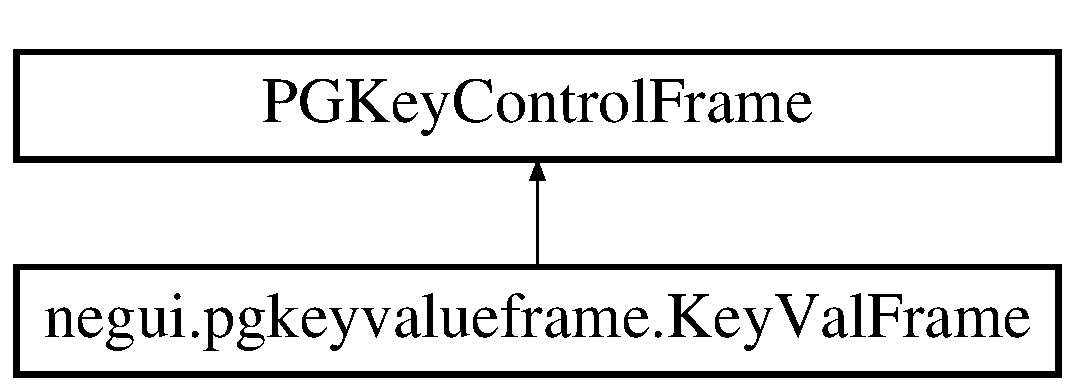
\includegraphics[height=2.000000cm]{classnegui_1_1pgkeyvalueframe_1_1KeyValFrame}
\end{center}
\end{figure}
\subsection*{Public Member Functions}
\begin{DoxyCompactItemize}
\item 
def \hyperlink{classnegui_1_1pgkeyvalueframe_1_1KeyValFrame_a8c2ff5749913d769fe35bb0022d92321}{\+\_\+\+\_\+init\+\_\+\+\_\+} (self, s\+\_\+name, v\+\_\+value, o\+\_\+type, v\+\_\+default\+\_\+value=None, o\+\_\+master=None, s\+\_\+associated\+\_\+attribute=None, o\+\_\+associated\+\_\+attribute\+\_\+object=None, i\+\_\+entrywidth=7, i\+\_\+labelwidth=15, b\+\_\+is\+\_\+enabled=True, s\+\_\+label\+\_\+justify=\textquotesingle{}right\textquotesingle{}, s\+\_\+entry\+\_\+justify=\textquotesingle{}right\textquotesingle{}, s\+\_\+button\+\_\+text=\textquotesingle{}Cmd\textquotesingle{}, def\+\_\+button\+\_\+command=None, def\+\_\+entry\+\_\+change\+\_\+command=None, type\+\_\+replaces\+\_\+none=float, s\+\_\+label\+\_\+name=None, i\+\_\+subframe\+\_\+padding=0, o\+\_\+validity\+\_\+tester=None, b\+\_\+force\+\_\+disable=False, s\+\_\+tooltip=None, b\+\_\+use\+\_\+list\+\_\+editor=False, i\+\_\+entry\+\_\+row=0, i\+\_\+entry\+\_\+col=1, i\+\_\+label\+\_\+row=0, i\+\_\+label\+\_\+col=0)
\item 
def {\bfseries manually\+Update\+Value} (self, v\+\_\+value, i\+\_\+idx=0)\hypertarget{classnegui_1_1pgkeyvalueframe_1_1KeyValFrame_a59b56809197ca8e3930e1ea07953d953}{}\label{classnegui_1_1pgkeyvalueframe_1_1KeyValFrame_a59b56809197ca8e3930e1ea07953d953}

\item 
def \hyperlink{classnegui_1_1pgkeyvalueframe_1_1KeyValFrame_adcbafb75f2a411d6a10c1c4248395e02}{set\+State\+Controls} (self, s\+\_\+state)
\item 
def {\bfseries get\+Control\+States} (self)\hypertarget{classnegui_1_1pgkeyvalueframe_1_1KeyValFrame_a94977d29ae8033de0d6c5dfdd2efd39c}{}\label{classnegui_1_1pgkeyvalueframe_1_1KeyValFrame_a94977d29ae8033de0d6c5dfdd2efd39c}

\item 
def {\bfseries val} (self)\hypertarget{classnegui_1_1pgkeyvalueframe_1_1KeyValFrame_a9417797618926333757e68767bb74233}{}\label{classnegui_1_1pgkeyvalueframe_1_1KeyValFrame_a9417797618926333757e68767bb74233}

\item 
def {\bfseries val} (self)\hypertarget{classnegui_1_1pgkeyvalueframe_1_1KeyValFrame_a9417797618926333757e68767bb74233}{}\label{classnegui_1_1pgkeyvalueframe_1_1KeyValFrame_a9417797618926333757e68767bb74233}

\item 
def {\bfseries is\+\_\+enabled} (self)\hypertarget{classnegui_1_1pgkeyvalueframe_1_1KeyValFrame_a72501403a679b0ee3822cea7626bcff2}{}\label{classnegui_1_1pgkeyvalueframe_1_1KeyValFrame_a72501403a679b0ee3822cea7626bcff2}

\item 
def {\bfseries force\+\_\+disable} (self)\hypertarget{classnegui_1_1pgkeyvalueframe_1_1KeyValFrame_a09ba9b45311ca28cd4e975761542e3f9}{}\label{classnegui_1_1pgkeyvalueframe_1_1KeyValFrame_a09ba9b45311ca28cd4e975761542e3f9}

\end{DoxyCompactItemize}
\subsection*{Public Attributes}
\begin{DoxyCompactItemize}
\item 
{\bfseries label}\hypertarget{classnegui_1_1pgkeyvalueframe_1_1KeyValFrame_a530e52fc0ef515f23995721a12a023fe}{}\label{classnegui_1_1pgkeyvalueframe_1_1KeyValFrame_a530e52fc0ef515f23995721a12a023fe}

\end{DoxyCompactItemize}
\subsection*{Static Public Attributes}
\begin{DoxyCompactItemize}
\item 
bool {\bfseries V\+E\+R\+B\+O\+SE} = False\hypertarget{classnegui_1_1pgkeyvalueframe_1_1KeyValFrame_a87c8cf8185b7653b59fb4ee3722845f0}{}\label{classnegui_1_1pgkeyvalueframe_1_1KeyValFrame_a87c8cf8185b7653b59fb4ee3722845f0}

\end{DoxyCompactItemize}


\subsection{Detailed Description}
\begin{DoxyVerb}Description

Tkinter frame object that creates,
from left to right, a label, then 
one or more entry boxes, one entry box 
if the type is not "list", otherwise one 
entry box for each list item.

the instance stores changes in the value(s)
via callback on enter key.  The current
key/value state is delivered via a getValue

Optionally also updates a an attribute
in its master object, by name (using getattr)
whenever the entry box value is updated.

Optionally also places a button to the right
of the entry box or boxes, and calls a user-supplied
def whenever a box is updated.

2016_09_18

Revise by adding list editing functions.\end{DoxyVerb}
 

Definition at line 34 of file pgkeyvalueframe.\+py.



\subsection{Constructor \& Destructor Documentation}
\index{negui\+::pgkeyvalueframe\+::\+Key\+Val\+Frame@{negui\+::pgkeyvalueframe\+::\+Key\+Val\+Frame}!\+\_\+\+\_\+init\+\_\+\+\_\+@{\+\_\+\+\_\+init\+\_\+\+\_\+}}
\index{\+\_\+\+\_\+init\+\_\+\+\_\+@{\+\_\+\+\_\+init\+\_\+\+\_\+}!negui\+::pgkeyvalueframe\+::\+Key\+Val\+Frame@{negui\+::pgkeyvalueframe\+::\+Key\+Val\+Frame}}
\subsubsection[{\texorpdfstring{\+\_\+\+\_\+init\+\_\+\+\_\+(self, s\+\_\+name, v\+\_\+value, o\+\_\+type, v\+\_\+default\+\_\+value=\+None, o\+\_\+master=\+None, s\+\_\+associated\+\_\+attribute=\+None, o\+\_\+associated\+\_\+attribute\+\_\+object=\+None, i\+\_\+entrywidth=7, i\+\_\+labelwidth=15, b\+\_\+is\+\_\+enabled=\+True, s\+\_\+label\+\_\+justify=\textquotesingle{}right\textquotesingle{}, s\+\_\+entry\+\_\+justify=\textquotesingle{}right\textquotesingle{}, s\+\_\+button\+\_\+text=\textquotesingle{}\+Cmd\textquotesingle{}, def\+\_\+button\+\_\+command=\+None, def\+\_\+entry\+\_\+change\+\_\+command=\+None, type\+\_\+replaces\+\_\+none=float, s\+\_\+label\+\_\+name=\+None, i\+\_\+subframe\+\_\+padding=0, o\+\_\+validity\+\_\+tester=\+None, b\+\_\+force\+\_\+disable=\+False, s\+\_\+tooltip=\+None, b\+\_\+use\+\_\+list\+\_\+editor=\+False, i\+\_\+entry\+\_\+row=0, i\+\_\+entry\+\_\+col=1, i\+\_\+label\+\_\+row=0, i\+\_\+label\+\_\+col=0)}{__init__(self, s_name, v_value, o_type, v_default_value=None, o_master=None, s_associated_attribute=None, o_associated_attribute_object=None, i_entrywidth=7, i_labelwidth=15, b_is_enabled=True, s_label_justify='right', s_entry_justify='right', s_button_text='Cmd', def_button_command=None, def_entry_change_command=None, type_replaces_none=float, s_label_name=None, i_subframe_padding=0, o_validity_tester=None, b_force_disable=False, s_tooltip=None, b_use_list_editor=False, i_entry_row=0, i_entry_col=1, i_label_row=0, i_label_col=0)}}]{\setlength{\rightskip}{0pt plus 5cm}def negui.\+pgkeyvalueframe.\+Key\+Val\+Frame.\+\_\+\+\_\+init\+\_\+\+\_\+ (
\begin{DoxyParamCaption}
\item[{}]{self, }
\item[{}]{s\+\_\+name, }
\item[{}]{v\+\_\+value, }
\item[{}]{o\+\_\+type, }
\item[{}]{v\+\_\+default\+\_\+value = {\ttfamily None}, }
\item[{}]{o\+\_\+master = {\ttfamily None}, }
\item[{}]{s\+\_\+associated\+\_\+attribute = {\ttfamily None}, }
\item[{}]{o\+\_\+associated\+\_\+attribute\+\_\+object = {\ttfamily None}, }
\item[{}]{i\+\_\+entrywidth = {\ttfamily 7}, }
\item[{}]{i\+\_\+labelwidth = {\ttfamily 15}, }
\item[{}]{b\+\_\+is\+\_\+enabled = {\ttfamily True}, }
\item[{}]{s\+\_\+label\+\_\+justify = {\ttfamily \textquotesingle{}right\textquotesingle{}}, }
\item[{}]{s\+\_\+entry\+\_\+justify = {\ttfamily \textquotesingle{}right\textquotesingle{}}, }
\item[{}]{s\+\_\+button\+\_\+text = {\ttfamily \textquotesingle{}Cmd\textquotesingle{}}, }
\item[{}]{def\+\_\+button\+\_\+command = {\ttfamily None}, }
\item[{}]{def\+\_\+entry\+\_\+change\+\_\+command = {\ttfamily None}, }
\item[{}]{type\+\_\+replaces\+\_\+none = {\ttfamily float}, }
\item[{}]{s\+\_\+label\+\_\+name = {\ttfamily None}, }
\item[{}]{i\+\_\+subframe\+\_\+padding = {\ttfamily 0}, }
\item[{}]{o\+\_\+validity\+\_\+tester = {\ttfamily None}, }
\item[{}]{b\+\_\+force\+\_\+disable = {\ttfamily False}, }
\item[{}]{s\+\_\+tooltip = {\ttfamily None}, }
\item[{}]{b\+\_\+use\+\_\+list\+\_\+editor = {\ttfamily False}, }
\item[{}]{i\+\_\+entry\+\_\+row = {\ttfamily 0}, }
\item[{}]{i\+\_\+entry\+\_\+col = {\ttfamily 1}, }
\item[{}]{i\+\_\+label\+\_\+row = {\ttfamily 0}, }
\item[{}]{i\+\_\+label\+\_\+col = {\ttfamily 0}}
\end{DoxyParamCaption}
)}\hypertarget{classnegui_1_1pgkeyvalueframe_1_1KeyValFrame_a8c2ff5749913d769fe35bb0022d92321}{}\label{classnegui_1_1pgkeyvalueframe_1_1KeyValFrame_a8c2ff5749913d769fe35bb0022d92321}
\begin{DoxyVerb}Param s_name provides the label text.
param v_value is the current value to be set as the
value for this KeyValFrame instance.  Note
if the client suppliesa list, the type given
here will be that of each item in the list.
param o_type gives the type of the value, or, if
the value is a list, the type of the list items
(uniform type assumed for list items.
param v_default_value gives the value that will be used
if the v_value is a list and the list ListEditingSubframe
object is being used.  In this case, when the current v_value
has len==0, then when the user invokes the "extend" def
in the ListEditingSubframe instance, a new list appears with
the v_default value as the single list item.
Param o_master is the parent Tkinter object.
Param s_associated_attribute is the name of 
    attribute instance that can be accessed
    using "getattr", and that will be
    updated when the value is updated.
Param o_associated_attribute_object is the object whose attribute
    is to be unpdated when the value is updated.  If
    s_associated_attribute is not None, and this parameter
    is None, the attribute is presumed to be
    owned by the o_master object.
Param i_entrywidth gives the width of Entry widget(s).
Param i_labelwidth gives the width the the Label widget.
Param s_label_justify gives Label widget "justify" value.
Param s_entry_justify gives Entry Widget text "justify" value.
Param s_butten_text gives the Button Widget's text value.
Param def_button_command gives the def to set to the Button's "command" param.
Param def_entry_change_command gives a def to call when the value of an entry is changed.             
      it should be used when an attribute is asssociated with this object,
      and so is automatically updated, after which some other action is required 
      (ex: Parent PGGuiSimuPop object needs to reconstiture the PGOutputSimuPop object 
      after this object updates its output basename attribute.
Param type_replaces_none: if a value is initially None, and the value is then updated, 
      this parameter.
      gives the type required for a valid value.
Param s_label_name, if supplied, replaces s_name as the text for the label.
Param i_subframe_padding gives the padding in pixels of the subframe inside its master frame
Param o_validity_tester, an object of class type ValueValidator or FloatIntStringParamValidity,
      (the latter class may be deprecated). If supplied, the KeyValFrame will use it to test all
      input values into an entry box, and disallow, with error message, when invalid values are
      entered. For class details see module pgutilityclasses.py
Param b_force_disable, if True, will cause all Entry objects to be disabled 
      in the def __make_entry
Param b_use_list_editor, if True, and if param v_value (see above) is passed as a list, 
      then a ListEditingSubframe object will be instantiated, allowing a GUI user to
      trim, extend, or assign one value to a range of list indices.
Param i_entry_row, integer, grid row at which to layout the entry or entries.
Param i_entry_col, integer, grid column at which to layout the first entry (incrementing for otherentries).
note that when a button is present, this will be it's column number, the entries following. 
Param i_label_row, integer, grid row at which to layout the label.
Param i_label_col, integer, grid column at which to layout the label.
\end{DoxyVerb}
 

Definition at line 91 of file pgkeyvalueframe.\+py.


\begin{DoxyCode}
91                     i\_label\_col=0 ):
92         
93         \textcolor{stringliteral}{"""}
94 \textcolor{stringliteral}{        Param s\_name provides the label text.}
95 \textcolor{stringliteral}{        param v\_value is the current value to be set as the}
96 \textcolor{stringliteral}{                value for this KeyValFrame instance.  Note}
97 \textcolor{stringliteral}{                if the client suppliesa list, the type given}
98 \textcolor{stringliteral}{                here will be that of each item in the list.}
99 \textcolor{stringliteral}{        param o\_type gives the type of the value, or, if}
100 \textcolor{stringliteral}{                the value is a list, the type of the list items}
101 \textcolor{stringliteral}{                (uniform type assumed for list items.}
102 \textcolor{stringliteral}{        param v\_default\_value gives the value that will be used}
103 \textcolor{stringliteral}{                if the v\_value is a list and the list ListEditingSubframe}
104 \textcolor{stringliteral}{                object is being used.  In this case, when the current v\_value}
105 \textcolor{stringliteral}{                has len==0, then when the user invokes the "extend" def}
106 \textcolor{stringliteral}{                in the ListEditingSubframe instance, a new list appears with}
107 \textcolor{stringliteral}{                the v\_default value as the single list item.}
108 \textcolor{stringliteral}{        Param o\_master is the parent Tkinter object.}
109 \textcolor{stringliteral}{        Param s\_associated\_attribute is the name of }
110 \textcolor{stringliteral}{            attribute instance that can be accessed}
111 \textcolor{stringliteral}{            using "getattr", and that will be}
112 \textcolor{stringliteral}{            updated when the value is updated.}
113 \textcolor{stringliteral}{        Param o\_associated\_attribute\_object is the object whose attribute}
114 \textcolor{stringliteral}{            is to be unpdated when the value is updated.  If}
115 \textcolor{stringliteral}{            s\_associated\_attribute is not None, and this parameter}
116 \textcolor{stringliteral}{            is None, the attribute is presumed to be}
117 \textcolor{stringliteral}{            owned by the o\_master object.}
118 \textcolor{stringliteral}{        Param i\_entrywidth gives the width of Entry widget(s).}
119 \textcolor{stringliteral}{        Param i\_labelwidth gives the width the the Label widget.}
120 \textcolor{stringliteral}{        Param s\_label\_justify gives Label widget "justify" value.}
121 \textcolor{stringliteral}{        Param s\_entry\_justify gives Entry Widget text "justify" value.}
122 \textcolor{stringliteral}{        Param s\_butten\_text gives the Button Widget's text value.}
123 \textcolor{stringliteral}{        Param def\_button\_command gives the def to set to the Button's "command" param.}
124 \textcolor{stringliteral}{        Param def\_entry\_change\_command gives a def to call when the value of an entry is changed.           
        }
125 \textcolor{stringliteral}{              it should be used when an attribute is asssociated with this object,}
126 \textcolor{stringliteral}{              and so is automatically updated, after which some other action is required }
127 \textcolor{stringliteral}{              (ex: Parent PGGuiSimuPop object needs to reconstiture the PGOutputSimuPop object }
128 \textcolor{stringliteral}{              after this object updates its output basename attribute.}
129 \textcolor{stringliteral}{        Param type\_replaces\_none: if a value is initially None, and the value is then updated, }
130 \textcolor{stringliteral}{              this parameter.}
131 \textcolor{stringliteral}{              gives the type required for a valid value.}
132 \textcolor{stringliteral}{        Param s\_label\_name, if supplied, replaces s\_name as the text for the label.}
133 \textcolor{stringliteral}{        Param i\_subframe\_padding gives the padding in pixels of the subframe inside its master frame}
134 \textcolor{stringliteral}{        Param o\_validity\_tester, an object of class type ValueValidator or FloatIntStringParamValidity,}
135 \textcolor{stringliteral}{              (the latter class may be deprecated). If supplied, the KeyValFrame will use it to test all}
136 \textcolor{stringliteral}{              input values into an entry box, and disallow, with error message, when invalid values are}
137 \textcolor{stringliteral}{              entered. For class details see module pgutilityclasses.py}
138 \textcolor{stringliteral}{        Param b\_force\_disable, if True, will cause all Entry objects to be disabled }
139 \textcolor{stringliteral}{              in the def \_\_make\_entry}
140 \textcolor{stringliteral}{        Param b\_use\_list\_editor, if True, and if param v\_value (see above) is passed as a list, }
141 \textcolor{stringliteral}{              then a ListEditingSubframe object will be instantiated, allowing a GUI user to}
142 \textcolor{stringliteral}{              trim, extend, or assign one value to a range of list indices.}
143 \textcolor{stringliteral}{        Param i\_entry\_row, integer, grid row at which to layout the entry or entries.}
144 \textcolor{stringliteral}{        Param i\_entry\_col, integer, grid column at which to layout the first entry (incrementing for
       otherentries).}
145 \textcolor{stringliteral}{                note that when a button is present, this will be it's column number, the entries following.
       }
146 \textcolor{stringliteral}{        Param i\_label\_row, integer, grid row at which to layout the label.}
147 \textcolor{stringliteral}{        Param i\_label\_col, integer, grid column at which to layout the label.}
148 \textcolor{stringliteral}{        """}
149 
150         PGKeyControlFrame.\_\_init\_\_( self, o\_master, name=s\_name.lower() )
151 
152         self.\hyperlink{classnegui_1_1pgkeyvalueframe_1_1KeyValFrame_a805253b977c0f43cdcf6ec5de53f14eb}{\_\_master}=o\_master
153         \textcolor{stringliteral}{'''}
154 \textcolor{stringliteral}{        This boolean var will be  reassigned}
155 \textcolor{stringliteral}{        if the client passed a list instead of an}
156 \textcolor{stringliteral}{        atomic type.  If true it will be reassigned}
157 \textcolor{stringliteral}{        in def \_\_store\_value:}
158 \textcolor{stringliteral}{        '''}
159         self.\hyperlink{classnegui_1_1pgkeyvalueframe_1_1KeyValFrame_af0631789b0da26d580e7079d6bcf14f1}{\_\_orig\_value\_is\_list}=\textcolor{keyword}{False}
160         \textcolor{comment}{#Holds updated value, intiialized}
161         \textcolor{comment}{#in def \_\_store\_value}
162         self.\hyperlink{classnegui_1_1pgkeyvalueframe_1_1KeyValFrame_a340fbacda4aba3bab65394922998d5a3}{\_\_value}=\textcolor{keywordtype}{None}
163         self.\hyperlink{classnegui_1_1pgkeyvalueframe_1_1KeyValFrame_ad5f6e2d38d7229b7e0cd23e2ab2fea2b}{\_\_default\_value}=v\_default\_value
164         self.\hyperlink{classnegui_1_1pgkeyvalueframe_1_1KeyValFrame_a5e972b92c19567f763da152f1d4b61dd}{\_\_value\_type}=o\_type
165         self.\hyperlink{classnegui_1_1pgkeyvalueframe_1_1KeyValFrame_a528d362ee685b490efe590679317ca7f}{\_\_store\_value}( v\_value )
166         self.\hyperlink{classnegui_1_1pgkeyvalueframe_1_1KeyValFrame_aecb3998429fcffea6ebb055d5f742963}{\_\_last\_state}=self.\hyperlink{classnegui_1_1pgkeyvalueframe_1_1KeyValFrame_a340fbacda4aba3bab65394922998d5a3}{\_\_value}
167         self.\hyperlink{classnegui_1_1pgkeyvalueframe_1_1KeyValFrame_a68f54607c216bc9ebbe00671b97583bc}{\_\_name}=s\_name
168         self.\hyperlink{classnegui_1_1pgkeyvalueframe_1_1KeyValFrame_a63f2490d3edbc674588303b57ae15aed}{\_\_entrywidth}=i\_entrywidth
169         self.\hyperlink{classnegui_1_1pgkeyvalueframe_1_1KeyValFrame_a98e43c4ade32564297bfbd138c39f6b5}{\_\_lablewidth}=i\_labelwidth
170         self.\hyperlink{classnegui_1_1pgkeyvalueframe_1_1KeyValFrame_a4f90f379a3925423d76e254e220d7cdb}{\_\_labeljustify}=s\_label\_justify
171         self.\hyperlink{classnegui_1_1pgkeyvalueframe_1_1KeyValFrame_a301c53dce29c99801cd41d85adc4cd5d}{\_\_entryjustify}=s\_entry\_justify
172         self.\hyperlink{classnegui_1_1pgkeyvalueframe_1_1KeyValFrame_a96a6ee2c2af530d26583687d6ad4f75e}{\_\_isenabled}=b\_is\_enabled
173         self.\hyperlink{classnegui_1_1pgkeyvalueframe_1_1KeyValFrame_a816407ab766176b96c4704e6b04ae093}{\_\_associated\_attribute}=s\_associated\_attribute
174         self.\hyperlink{classnegui_1_1pgkeyvalueframe_1_1KeyValFrame_a3bc7265c401db26785fea8c9502a2174}{\_\_associated\_attribute\_object}=o\_associated\_attribute\_object
175         self.\hyperlink{classnegui_1_1pgkeyvalueframe_1_1KeyValFrame_a5eff25aa85ba087f16db456640ea8761}{\_\_button\_text}=s\_button\_text
176         self.\hyperlink{classnegui_1_1pgkeyvalueframe_1_1KeyValFrame_a4b8c159a633099f4c76052e529397739}{\_\_button\_command}=def\_button\_command
177         self.\hyperlink{classnegui_1_1pgkeyvalueframe_1_1KeyValFrame_a0d58985493ae76e481c31574fd813419}{\_\_entry\_change\_command}=def\_entry\_change\_command
178         self.\hyperlink{classnegui_1_1pgkeyvalueframe_1_1KeyValFrame_ad175bbdb1a94e72cd2e0c1d9482fd2a3}{\_\_type\_replaces\_none}=type\_replaces\_none
179         self.\hyperlink{classnegui_1_1pgkeyvalueframe_1_1KeyValFrame_af3f6f22fcd9bc5d4f3633b74169a84e1}{\_\_subframe\_padding}=i\_subframe\_padding
180         self.\hyperlink{classnegui_1_1pgkeyvalueframe_1_1KeyValFrame_a78f462eeca767880558b8e9ae7e4dbb9}{\_\_validity\_tester}=o\_validity\_tester
181         self.\hyperlink{classnegui_1_1pgkeyvalueframe_1_1KeyValFrame_a60d7b1c6d172090d4944d51773bf3092}{\_\_force\_disable}=b\_force\_disable
182         self.\hyperlink{classnegui_1_1pgkeyvalueframe_1_1KeyValFrame_a556d790da8f00002869fbf8cbb1679ad}{\_\_entry\_row}=i\_entry\_row
183         self.\hyperlink{classnegui_1_1pgkeyvalueframe_1_1KeyValFrame_abf71508b243fa605394904b6a960a45e}{\_\_entry\_col}=i\_entry\_col
184         self.\hyperlink{classnegui_1_1pgkeyvalueframe_1_1KeyValFrame_a4f82cb8aeb73bb76bbf1865703c3d5fa}{\_\_label\_row}=i\_label\_row
185         self.\hyperlink{classnegui_1_1pgkeyvalueframe_1_1KeyValFrame_a1e5e52ab782cf38622a8afdbd1dc00ed}{\_\_label\_col}=i\_label\_col
186         self.\hyperlink{classnegui_1_1pgkeyvalueframe_1_1KeyValFrame_ad0c9f91eee034c840986295b8da19b39}{\_\_idx\_none\_values}=[]
187         self.\hyperlink{classnegui_1_1pgkeyvalueframe_1_1KeyValFrame_aa97b894ebab00acf5ff007395d30eb35}{\_\_entryvals}=[]
188         
189         self.\hyperlink{classnegui_1_1pgkeyvalueframe_1_1KeyValFrame_a07f6a4307c96a10510baa41467730898}{\_\_label\_name}=s\_name \textcolor{keywordflow}{if} s\_label\_name \textcolor{keywordflow}{is} \textcolor{keywordtype}{None} \(\backslash\)
190                                             \textcolor{keywordflow}{else} s\_label\_name       
191         \textcolor{comment}{#end if no label name, use name, else use label}
192 
193         \textcolor{stringliteral}{'''}
194 \textcolor{stringliteral}{        If the value is passed as a list (see def \_\_store\_value)}
195 \textcolor{stringliteral}{        and this param was passed as True in the \_\_init\_\_ args,}
196 \textcolor{stringliteral}{        a ListEditingSubframe instance will be created:}
197 \textcolor{stringliteral}{        '''}
198         self.\hyperlink{classnegui_1_1pgkeyvalueframe_1_1KeyValFrame_ae88e690943610d54815c9a238b6d604d}{\_\_tooltip}=s\_tooltip \textcolor{keywordflow}{if} s\_tooltip \textcolor{keywordflow}{is} \textcolor{keywordflow}{not} \textcolor{keywordtype}{None} \(\backslash\)
199                                         \textcolor{keywordflow}{else} self.\hyperlink{classnegui_1_1pgkeyvalueframe_1_1KeyValFrame_a07f6a4307c96a10510baa41467730898}{\_\_label\_name}
200 
201         self.\hyperlink{classnegui_1_1pgkeyvalueframe_1_1KeyValFrame_aa0a47e8756fbd3228291a3594955cb04}{\_\_use\_list\_editor}=b\_use\_list\_editor
202 
203         \textcolor{comment}{#ListEditingSubframe object created if}
204         \textcolor{comment}{#our value as passed by client is a list:}
205         self.\hyperlink{classnegui_1_1pgkeyvalueframe_1_1KeyValFrame_a17e8b612d13e5c6bbb28774eb672780a}{\_\_list\_editor}=\textcolor{keywordtype}{None}
206 
207         \textcolor{comment}{#references to the tkinter controls}
208         \textcolor{comment}{#that may be subject to config}
209         \textcolor{comment}{#after init:}
210         self.\hyperlink{classnegui_1_1pgkeyvalueframe_1_1KeyValFrame_a7eafad6669c78425aa94fe5ac1cda138}{\_\_entry\_boxes}=[]
211         self.\hyperlink{classnegui_1_1pgkeyvalueframe_1_1KeyValFrame_a7e6fd366dcf788ba3aeaadbc20eef128}{\_\_textvariables}=[]
212         self.\hyperlink{classnegui_1_1pgkeyvalueframe_1_1KeyValFrame_a74876c723f1477e8fe903f8ef03d9352}{\_\_button\_object}=\textcolor{keywordtype}{None}
213 
214         \textcolor{comment}{#Canvas, Frame, and other attributes}
215         \textcolor{comment}{#that will allow scrolling and correct}
216         \textcolor{comment}{#resizing (see def \_\_setup\_subwidgets)}
217         self.\hyperlink{classnegui_1_1pgkeyvalueframe_1_1KeyValFrame_ada8d64cd3936f223d32929b37a818eb0}{\_\_canvas}=\textcolor{keywordtype}{None}
218         self.\hyperlink{classnegui_1_1pgkeyvalueframe_1_1KeyValFrame_a2038af0d44c2075ee52400ca849e0974}{\_\_subframe}=\textcolor{keywordtype}{None}
219         self.\hyperlink{classnegui_1_1pgkeyvalueframe_1_1KeyValFrame_abe8598381772872d5d676189baa676a4}{\_\_subframe\_id}=\textcolor{keywordtype}{None}
220         
221         self.\hyperlink{classnegui_1_1pgkeyvalueframe_1_1KeyValFrame_ac4c3b92c3dc6a58b7b50ea0318be4579}{\_\_setup}()
222 
\end{DoxyCode}


\subsection{Member Function Documentation}
\index{negui\+::pgkeyvalueframe\+::\+Key\+Val\+Frame@{negui\+::pgkeyvalueframe\+::\+Key\+Val\+Frame}!set\+State\+Controls@{set\+State\+Controls}}
\index{set\+State\+Controls@{set\+State\+Controls}!negui\+::pgkeyvalueframe\+::\+Key\+Val\+Frame@{negui\+::pgkeyvalueframe\+::\+Key\+Val\+Frame}}
\subsubsection[{\texorpdfstring{set\+State\+Controls(self, s\+\_\+state)}{setStateControls(self, s_state)}}]{\setlength{\rightskip}{0pt plus 5cm}def negui.\+pgkeyvalueframe.\+Key\+Val\+Frame.\+set\+State\+Controls (
\begin{DoxyParamCaption}
\item[{}]{self, }
\item[{}]{s\+\_\+state}
\end{DoxyParamCaption}
)}\hypertarget{classnegui_1_1pgkeyvalueframe_1_1KeyValFrame_adcbafb75f2a411d6a10c1c4248395e02}{}\label{classnegui_1_1pgkeyvalueframe_1_1KeyValFrame_adcbafb75f2a411d6a10c1c4248395e02}
\begin{DoxyVerb}Set the state of all this objects
entry boxes and (if present) button
to the value passed.
\end{DoxyVerb}
 

Definition at line 699 of file pgkeyvalueframe.\+py.


\begin{DoxyCode}
699     \textcolor{keyword}{def }\hyperlink{classnegui_1_1pgkeyvalueframe_1_1KeyValFrame_adcbafb75f2a411d6a10c1c4248395e02}{setStateControls}( self, s\_state ):
700         \textcolor{stringliteral}{'''}
701 \textcolor{stringliteral}{        Set the state of all this objects}
702 \textcolor{stringliteral}{        entry boxes and (if present) button}
703 \textcolor{stringliteral}{        to the value passed.}
704 \textcolor{stringliteral}{        '''}
705 
706         self.\hyperlink{classnegui_1_1pgkeyvalueframe_1_1KeyValFrame_a96a6ee2c2af530d26583687d6ad4f75e}{\_\_isenabled}=( s\_state == \textcolor{stringliteral}{"enabled"} )
707 
708         \textcolor{keywordflow}{for} o\_entry\_box \textcolor{keywordflow}{in} self.\hyperlink{classnegui_1_1pgkeyvalueframe_1_1KeyValFrame_a7eafad6669c78425aa94fe5ac1cda138}{\_\_entry\_boxes}:
709             o\_entry\_box.configure( state=s\_state )
710         \textcolor{comment}{#end for each entry box}
711 
712         \textcolor{keywordflow}{if} self.\hyperlink{classnegui_1_1pgkeyvalueframe_1_1KeyValFrame_a74876c723f1477e8fe903f8ef03d9352}{\_\_button\_object} \textcolor{keywordflow}{is} \textcolor{keywordflow}{not} \textcolor{keywordtype}{None}:
713             self.\_\_button\_object.configure( state=s\_state )
714         \textcolor{comment}{#end if we have a button}
715 
716         \textcolor{keywordflow}{return}
\end{DoxyCode}


The documentation for this class was generated from the following file\+:\begin{DoxyCompactItemize}
\item 
pgkeyvalueframe.\+py\end{DoxyCompactItemize}

\hypertarget{classnegui_1_1pgutilityclasses_1_1LDNENbBiasAdjustor}{}\section{negui.\+pgutilityclasses.\+L\+D\+N\+E\+Nb\+Bias\+Adjustor Class Reference}
\label{classnegui_1_1pgutilityclasses_1_1LDNENbBiasAdjustor}\index{negui.\+pgutilityclasses.\+L\+D\+N\+E\+Nb\+Bias\+Adjustor@{negui.\+pgutilityclasses.\+L\+D\+N\+E\+Nb\+Bias\+Adjustor}}
Inheritance diagram for negui.\+pgutilityclasses.\+L\+D\+N\+E\+Nb\+Bias\+Adjustor\+:\begin{figure}[H]
\begin{center}
\leavevmode
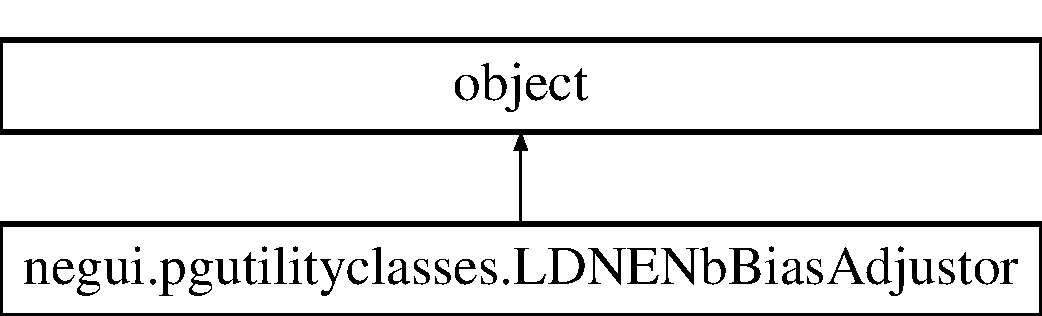
\includegraphics[height=2.000000cm]{classnegui_1_1pgutilityclasses_1_1LDNENbBiasAdjustor}
\end{center}
\end{figure}
\subsection*{Public Member Functions}
\begin{DoxyCompactItemize}
\item 
def {\bfseries \+\_\+\+\_\+init\+\_\+\+\_\+} (self, v\+\_\+original\+\_\+nb=None, f\+\_\+nbne\+\_\+ratio=None)\hypertarget{classnegui_1_1pgutilityclasses_1_1LDNENbBiasAdjustor_a4a55145de8b56fe28a8fe743b5f2bca0}{}\label{classnegui_1_1pgutilityclasses_1_1LDNENbBiasAdjustor_a4a55145de8b56fe28a8fe743b5f2bca0}

\item 
def {\bfseries adjusted\+\_\+nb} (self)\hypertarget{classnegui_1_1pgutilityclasses_1_1LDNENbBiasAdjustor_a68d259290d69c96c16b0f7231c928306}{}\label{classnegui_1_1pgutilityclasses_1_1LDNENbBiasAdjustor_a68d259290d69c96c16b0f7231c928306}

\item 
def {\bfseries original\+\_\+nb} (self)\hypertarget{classnegui_1_1pgutilityclasses_1_1LDNENbBiasAdjustor_a7ce9a8792818a6a187d9aca9689d3c0e}{}\label{classnegui_1_1pgutilityclasses_1_1LDNENbBiasAdjustor_a7ce9a8792818a6a187d9aca9689d3c0e}

\item 
def {\bfseries original\+\_\+nb} (self, v\+\_\+nb)\hypertarget{classnegui_1_1pgutilityclasses_1_1LDNENbBiasAdjustor_add7013606409d902879674323bd7b0c4}{}\label{classnegui_1_1pgutilityclasses_1_1LDNENbBiasAdjustor_add7013606409d902879674323bd7b0c4}

\item 
def {\bfseries nbne\+\_\+ratio} (self)\hypertarget{classnegui_1_1pgutilityclasses_1_1LDNENbBiasAdjustor_afd9f80d46c3fd89e3e38ae8ef1f3d71a}{}\label{classnegui_1_1pgutilityclasses_1_1LDNENbBiasAdjustor_afd9f80d46c3fd89e3e38ae8ef1f3d71a}

\item 
def {\bfseries nbne\+\_\+ratio} (self, f\+\_\+nbne\+\_\+ratio)\hypertarget{classnegui_1_1pgutilityclasses_1_1LDNENbBiasAdjustor_a1751127c7311f26ae36b083963591d7b}{}\label{classnegui_1_1pgutilityclasses_1_1LDNENbBiasAdjustor_a1751127c7311f26ae36b083963591d7b}

\end{DoxyCompactItemize}


\subsection{Detailed Description}
\begin{DoxyVerb}Wrapper around the bias adjustment as given in 
Waples, etal., "Effects of Overlapping Generations on Linkage 
Disequilibrium Estimates of Effective Population Size Genetics." 
Available at: 
http://www.genetics.org/content/early/2014/04/08/genetics.114.164822.
\end{DoxyVerb}
 

Definition at line 1082 of file pgutilityclasses.\+py.



The documentation for this class was generated from the following file\+:\begin{DoxyCompactItemize}
\item 
pgutilityclasses.\+py\end{DoxyCompactItemize}

\hypertarget{classnegui_1_1pglisteditingsubframe_1_1ListEditingSubframe}{}\section{negui.\+pglisteditingsubframe.\+List\+Editing\+Subframe Class Reference}
\label{classnegui_1_1pglisteditingsubframe_1_1ListEditingSubframe}\index{negui.\+pglisteditingsubframe.\+List\+Editing\+Subframe@{negui.\+pglisteditingsubframe.\+List\+Editing\+Subframe}}
Inheritance diagram for negui.\+pglisteditingsubframe.\+List\+Editing\+Subframe\+:\begin{figure}[H]
\begin{center}
\leavevmode
\includegraphics[height=2.000000cm]{classnegui_1_1pglisteditingsubframe_1_1ListEditingSubframe}
\end{center}
\end{figure}
\subsection*{Public Member Functions}
\begin{DoxyCompactItemize}
\item 
def {\bfseries \+\_\+\+\_\+init\+\_\+\+\_\+} (self, o\+\_\+master, lv\+\_\+list, def\+\_\+to\+\_\+call\+\_\+when\+\_\+list\+\_\+changes=None, v\+\_\+default\+\_\+value=0.\+0, s\+\_\+state=\char`\"{}enabled\char`\"{}, i\+\_\+control\+\_\+width=10, i\+\_\+button\+\_\+width=8, o\+\_\+acceptable\+\_\+item\+\_\+type=float, b\+\_\+allow\+\_\+none\+\_\+value\+\_\+for\+\_\+list=True)\hypertarget{classnegui_1_1pglisteditingsubframe_1_1ListEditingSubframe_a056dc8bac2539fcbd7f002e82adea393}{}\label{classnegui_1_1pglisteditingsubframe_1_1ListEditingSubframe_a056dc8bac2539fcbd7f002e82adea393}

\item 
def {\bfseries thelist} (self)\hypertarget{classnegui_1_1pglisteditingsubframe_1_1ListEditingSubframe_a752edbc23d998e0c07a787c2b13acbfa}{}\label{classnegui_1_1pglisteditingsubframe_1_1ListEditingSubframe_a752edbc23d998e0c07a787c2b13acbfa}

\item 
def {\bfseries thelist} (self, lv\+\_\+list)\hypertarget{classnegui_1_1pglisteditingsubframe_1_1ListEditingSubframe_a7ee2540c89f5c8c6d15f5ba8132cf2ce}{}\label{classnegui_1_1pglisteditingsubframe_1_1ListEditingSubframe_a7ee2540c89f5c8c6d15f5ba8132cf2ce}

\item 
def {\bfseries defaultvalue} (self)\hypertarget{classnegui_1_1pglisteditingsubframe_1_1ListEditingSubframe_aa385a1aa0cb6ffdbf3ab1d743fa5bf3a}{}\label{classnegui_1_1pglisteditingsubframe_1_1ListEditingSubframe_aa385a1aa0cb6ffdbf3ab1d743fa5bf3a}

\item 
def {\bfseries defaultvalue} (self, v\+\_\+value)\hypertarget{classnegui_1_1pglisteditingsubframe_1_1ListEditingSubframe_a3670d218aa119b54a3e29d7e6b0792e2}{}\label{classnegui_1_1pglisteditingsubframe_1_1ListEditingSubframe_a3670d218aa119b54a3e29d7e6b0792e2}

\end{DoxyCompactItemize}
\subsection*{Public Attributes}
\begin{DoxyCompactItemize}
\item 
{\bfseries B\+T\+N\+\_\+\+C\+O\+L\+\_\+\+E\+X\+T\+E\+ND}\hypertarget{classnegui_1_1pglisteditingsubframe_1_1ListEditingSubframe_ad5ae3b4749d334d38a283f75a35ffea0}{}\label{classnegui_1_1pglisteditingsubframe_1_1ListEditingSubframe_ad5ae3b4749d334d38a283f75a35ffea0}

\item 
{\bfseries B\+T\+N\+\_\+\+C\+O\+L\+\_\+\+T\+R\+IM}\hypertarget{classnegui_1_1pglisteditingsubframe_1_1ListEditingSubframe_a25820548e892e070f856434b9a1a1c16}{}\label{classnegui_1_1pglisteditingsubframe_1_1ListEditingSubframe_a25820548e892e070f856434b9a1a1c16}

\item 
{\bfseries L\+A\+B\+E\+L\+\_\+\+C\+O\+L\+\_\+\+A\+S\+S\+I\+GN}\hypertarget{classnegui_1_1pglisteditingsubframe_1_1ListEditingSubframe_a4883b4b102b824dd56510d8e58711d9b}{}\label{classnegui_1_1pglisteditingsubframe_1_1ListEditingSubframe_a4883b4b102b824dd56510d8e58711d9b}

\item 
{\bfseries E\+N\+T\+R\+Y\+\_\+\+C\+O\+L\+\_\+\+F\+R\+OM}\hypertarget{classnegui_1_1pglisteditingsubframe_1_1ListEditingSubframe_ad85dea91fa2b6d472b40109843a8dc57}{}\label{classnegui_1_1pglisteditingsubframe_1_1ListEditingSubframe_ad85dea91fa2b6d472b40109843a8dc57}

\item 
{\bfseries L\+A\+B\+E\+L\+\_\+\+C\+O\+L\+\_\+\+TO}\hypertarget{classnegui_1_1pglisteditingsubframe_1_1ListEditingSubframe_ab8539d40b70f45c2d10825db62490797}{}\label{classnegui_1_1pglisteditingsubframe_1_1ListEditingSubframe_ab8539d40b70f45c2d10825db62490797}

\item 
{\bfseries E\+N\+T\+R\+Y\+\_\+\+C\+O\+L\+\_\+\+TO}\hypertarget{classnegui_1_1pglisteditingsubframe_1_1ListEditingSubframe_a2cef2374e75673eec9150c0ff3702684}{}\label{classnegui_1_1pglisteditingsubframe_1_1ListEditingSubframe_a2cef2374e75673eec9150c0ff3702684}

\item 
{\bfseries L\+A\+B\+E\+L\+\_\+\+C\+O\+L\+\_\+\+V\+A\+L\+UE}\hypertarget{classnegui_1_1pglisteditingsubframe_1_1ListEditingSubframe_abf2d74a2375126e8c96c6e8c592c6faa}{}\label{classnegui_1_1pglisteditingsubframe_1_1ListEditingSubframe_abf2d74a2375126e8c96c6e8c592c6faa}

\item 
{\bfseries E\+N\+T\+R\+Y\+\_\+\+C\+O\+L\+\_\+\+V\+A\+L\+UE}\hypertarget{classnegui_1_1pglisteditingsubframe_1_1ListEditingSubframe_aed6da663d989087c187fff50769f90e2}{}\label{classnegui_1_1pglisteditingsubframe_1_1ListEditingSubframe_aed6da663d989087c187fff50769f90e2}

\item 
{\bfseries B\+T\+N\+\_\+\+C\+O\+L\+\_\+\+A\+S\+S\+I\+GN}\hypertarget{classnegui_1_1pglisteditingsubframe_1_1ListEditingSubframe_a67e8a78c5364e0adfe24e881f5c7891f}{}\label{classnegui_1_1pglisteditingsubframe_1_1ListEditingSubframe_a67e8a78c5364e0adfe24e881f5c7891f}

\item 
{\bfseries T\+O\+T\+A\+L\+\_\+\+C\+O\+N\+T\+R\+O\+LS}\hypertarget{classnegui_1_1pglisteditingsubframe_1_1ListEditingSubframe_ad63121db3667ca83f5f565b8a0a16e9b}{}\label{classnegui_1_1pglisteditingsubframe_1_1ListEditingSubframe_ad63121db3667ca83f5f565b8a0a16e9b}

\end{DoxyCompactItemize}


\subsection{Detailed Description}
\begin{DoxyVerb}2016_09_18

A frame with gui controls to add or trim
an item from a list, or to assign a single
value to a range of list indices.  

This class created as a subframe to sit
below a list of items in a KeyValFrame
instance whose client passed a list into
the KeyValFrame.  Because trimming and extending
a list are not easily implemented in the current
KeyValFrame class, and because values in the displayed
list are only editable one at a time, this
class is meant to offer them (in a basic form). 

Note that this class would be unneccesary if Tkinter
has a sreadsheet-like widget.

2016_10_31 
Because I'm currently not using the assign-range, 
funcion, and, although it seems to be working, it nonetheless
complicates the communications between this class objectd
and its parent KeyValFrame, I'm for now going to hide these
controls. See def __setup, where I've commented out the
grid assignments of the assign-range controls.
\end{DoxyVerb}
 

Definition at line 22 of file pglisteditingsubframe.\+py.



The documentation for this class was generated from the following file\+:\begin{DoxyCompactItemize}
\item 
pglisteditingsubframe.\+py\end{DoxyCompactItemize}

\hypertarget{classnegui_1_1pgkeycheckboxvalueframe_1_1myattr}{}\section{negui.\+pgkeycheckboxvalueframe.\+myattr Class Reference}
\label{classnegui_1_1pgkeycheckboxvalueframe_1_1myattr}\index{negui.\+pgkeycheckboxvalueframe.\+myattr@{negui.\+pgkeycheckboxvalueframe.\+myattr}}
Inheritance diagram for negui.\+pgkeycheckboxvalueframe.\+myattr\+:\begin{figure}[H]
\begin{center}
\leavevmode
\includegraphics[height=2.000000cm]{classnegui_1_1pgkeycheckboxvalueframe_1_1myattr}
\end{center}
\end{figure}
\subsection*{Public Member Functions}
\begin{DoxyCompactItemize}
\item 
def {\bfseries \+\_\+\+\_\+init\+\_\+\+\_\+} (self, vval=False)\hypertarget{classnegui_1_1pgkeycheckboxvalueframe_1_1myattr_a6130ccf2471559655c3b4ecfe09d43d5}{}\label{classnegui_1_1pgkeycheckboxvalueframe_1_1myattr_a6130ccf2471559655c3b4ecfe09d43d5}

\end{DoxyCompactItemize}
\subsection*{Public Attributes}
\begin{DoxyCompactItemize}
\item 
{\bfseries vval}\hypertarget{classnegui_1_1pgkeycheckboxvalueframe_1_1myattr_a2e3ac14c8f3febe2a11f47706175891c}{}\label{classnegui_1_1pgkeycheckboxvalueframe_1_1myattr_a2e3ac14c8f3febe2a11f47706175891c}

\end{DoxyCompactItemize}


\subsection{Detailed Description}


Definition at line 272 of file pgkeycheckboxvalueframe.\+py.



The documentation for this class was generated from the following file\+:\begin{DoxyCompactItemize}
\item 
pgkeycheckboxvalueframe.\+py\end{DoxyCompactItemize}

\hypertarget{classnegui_1_1pgutilityclasses_1_1NbAdjustmentRangeAndRate}{}\section{negui.\+pgutilityclasses.\+Nb\+Adjustment\+Range\+And\+Rate Class Reference}
\label{classnegui_1_1pgutilityclasses_1_1NbAdjustmentRangeAndRate}\index{negui.\+pgutilityclasses.\+Nb\+Adjustment\+Range\+And\+Rate@{negui.\+pgutilityclasses.\+Nb\+Adjustment\+Range\+And\+Rate}}
Inheritance diagram for negui.\+pgutilityclasses.\+Nb\+Adjustment\+Range\+And\+Rate\+:\begin{figure}[H]
\begin{center}
\leavevmode
\includegraphics[height=2.000000cm]{classnegui_1_1pgutilityclasses_1_1NbAdjustmentRangeAndRate}
\end{center}
\end{figure}
\subsection*{Public Member Functions}
\begin{DoxyCompactItemize}
\item 
def {\bfseries \+\_\+\+\_\+init\+\_\+\+\_\+} (self, i\+\_\+min\+\_\+valid\+\_\+cycle, i\+\_\+max\+\_\+valid\+\_\+cycle, s\+\_\+range\+\_\+as\+\_\+string=None)\hypertarget{classnegui_1_1pgutilityclasses_1_1NbAdjustmentRangeAndRate_a6c22de41e6755accc4c9878ac714c8db}{}\label{classnegui_1_1pgutilityclasses_1_1NbAdjustmentRangeAndRate_a6c22de41e6755accc4c9878ac714c8db}

\item 
def {\bfseries is\+Valid\+Range} (self, i\+\_\+start, i\+\_\+end)\hypertarget{classnegui_1_1pgutilityclasses_1_1NbAdjustmentRangeAndRate_a99a77b4405eb93b37788cd238c9e7504}{}\label{classnegui_1_1pgutilityclasses_1_1NbAdjustmentRangeAndRate_a99a77b4405eb93b37788cd238c9e7504}

\item 
def {\bfseries is\+Valid\+Cycle\+Number} (self, i\+\_\+number)\hypertarget{classnegui_1_1pgutilityclasses_1_1NbAdjustmentRangeAndRate_ab0770eaae9e2a95554aee493d5c235a3}{}\label{classnegui_1_1pgutilityclasses_1_1NbAdjustmentRangeAndRate_ab0770eaae9e2a95554aee493d5c235a3}

\item 
def {\bfseries set\+Range\+And\+Rate} (self, s\+\_\+string)\hypertarget{classnegui_1_1pgutilityclasses_1_1NbAdjustmentRangeAndRate_a9b7441041bd80281f44e24ade3470c9f}{}\label{classnegui_1_1pgutilityclasses_1_1NbAdjustmentRangeAndRate_a9b7441041bd80281f44e24ade3470c9f}

\item 
def {\bfseries start\+\_\+cycle} (self)\hypertarget{classnegui_1_1pgutilityclasses_1_1NbAdjustmentRangeAndRate_a090215270434fee82431a0c9a59cf35a}{}\label{classnegui_1_1pgutilityclasses_1_1NbAdjustmentRangeAndRate_a090215270434fee82431a0c9a59cf35a}

\item 
def {\bfseries end\+\_\+cycle} (self)\hypertarget{classnegui_1_1pgutilityclasses_1_1NbAdjustmentRangeAndRate_a97e299bb098b2da8a022e62d6e9b1bbb}{}\label{classnegui_1_1pgutilityclasses_1_1NbAdjustmentRangeAndRate_a97e299bb098b2da8a022e62d6e9b1bbb}

\item 
def {\bfseries rate} (self)\hypertarget{classnegui_1_1pgutilityclasses_1_1NbAdjustmentRangeAndRate_aa8ee83b9c730cc0ee925a7b59ad7ac60}{}\label{classnegui_1_1pgutilityclasses_1_1NbAdjustmentRangeAndRate_aa8ee83b9c730cc0ee925a7b59ad7ac60}

\end{DoxyCompactItemize}


\subsection{Detailed Description}
\begin{DoxyVerb}2017_03_07.  Class to convert a string of the form m[-n]:r
into two integers giving a start and end cycle number,
and a float giving a rate for reducing/augmenting
Nb (and Nc) by that rate over the given range of simulation 
(breeding) cycles.  If string has form m:r, then the range 
is restricted to the nth cycle.  Otherwise, given m-n:r, 
the cycle range is set as cycles m to n.\end{DoxyVerb}
 

Definition at line 1217 of file pgutilityclasses.\+py.



The documentation for this class was generated from the following file\+:\begin{DoxyCompactItemize}
\item 
pgutilityclasses.\+py\end{DoxyCompactItemize}

\hypertarget{classnegui_1_1pgutilityclasses_1_1NbNeReader}{}\section{negui.\+pgutilityclasses.\+Nb\+Ne\+Reader Class Reference}
\label{classnegui_1_1pgutilityclasses_1_1NbNeReader}\index{negui.\+pgutilityclasses.\+Nb\+Ne\+Reader@{negui.\+pgutilityclasses.\+Nb\+Ne\+Reader}}
Inheritance diagram for negui.\+pgutilityclasses.\+Nb\+Ne\+Reader\+:\begin{figure}[H]
\begin{center}
\leavevmode
\includegraphics[height=2.000000cm]{classnegui_1_1pgutilityclasses_1_1NbNeReader}
\end{center}
\end{figure}
\subsection*{Public Member Functions}
\begin{DoxyCompactItemize}
\item 
def \hyperlink{classnegui_1_1pgutilityclasses_1_1NbNeReader_ad4dbe99a948ee4133ced448874060e94}{\+\_\+\+\_\+init\+\_\+\+\_\+} (self, v\+\_\+genepop\+\_\+file)
\item 
def {\bfseries nbne\+\_\+ratio} (self)\hypertarget{classnegui_1_1pgutilityclasses_1_1NbNeReader_a353d1b38373b5ba51e72cff5d605b032}{}\label{classnegui_1_1pgutilityclasses_1_1NbNeReader_a353d1b38373b5ba51e72cff5d605b032}

\end{DoxyCompactItemize}
\subsection*{Static Public Attributes}
\begin{DoxyCompactItemize}
\item 
{\bfseries N\+O\+\_\+\+R\+A\+T\+IO} = None\hypertarget{classnegui_1_1pgutilityclasses_1_1NbNeReader_a56d113bf03742b060487869f004f5d60}{}\label{classnegui_1_1pgutilityclasses_1_1NbNeReader_a56d113bf03742b060487869f004f5d60}

\end{DoxyCompactItemize}


\subsection{Detailed Description}
\begin{DoxyVerb}2017_04_17.  This class is used to check the header line of a
Genepop file for a terminating string of the form, "nbne=r", where
r is a float giving an Nb/Ne ratio.  Genepop file generated using our
pgop, pginput and pgoutput simupop driving modules will store the 
value suchwise.  If the value stored in the header is very close
to zero (see def __read_nbne_ratio), then the __nbne_ratio will
be set to NO_RATIO (curently = None).
\end{DoxyVerb}
 

Definition at line 1359 of file pgutilityclasses.\+py.



\subsection{Constructor \& Destructor Documentation}
\index{negui\+::pgutilityclasses\+::\+Nb\+Ne\+Reader@{negui\+::pgutilityclasses\+::\+Nb\+Ne\+Reader}!\+\_\+\+\_\+init\+\_\+\+\_\+@{\+\_\+\+\_\+init\+\_\+\+\_\+}}
\index{\+\_\+\+\_\+init\+\_\+\+\_\+@{\+\_\+\+\_\+init\+\_\+\+\_\+}!negui\+::pgutilityclasses\+::\+Nb\+Ne\+Reader@{negui\+::pgutilityclasses\+::\+Nb\+Ne\+Reader}}
\subsubsection[{\texorpdfstring{\+\_\+\+\_\+init\+\_\+\+\_\+(self, v\+\_\+genepop\+\_\+file)}{__init__(self, v_genepop_file)}}]{\setlength{\rightskip}{0pt plus 5cm}def negui.\+pgutilityclasses.\+Nb\+Ne\+Reader.\+\_\+\+\_\+init\+\_\+\+\_\+ (
\begin{DoxyParamCaption}
\item[{}]{self, }
\item[{}]{v\+\_\+genepop\+\_\+file}
\end{DoxyParamCaption}
)}\hypertarget{classnegui_1_1pgutilityclasses_1_1NbNeReader_ad4dbe99a948ee4133ced448874060e94}{}\label{classnegui_1_1pgutilityclasses_1_1NbNeReader_ad4dbe99a948ee4133ced448874060e94}
\begin{DoxyVerb}Param v_genepopfile_manager_object should be either,
    --A string giving the name of a genepop file, or, 
    --A GenepopFileManager object.
\end{DoxyVerb}
 

Definition at line 1373 of file pgutilityclasses.\+py.


\begin{DoxyCode}
1373     \textcolor{keyword}{def }\hyperlink{classnegui_1_1pgutilityclasses_1_1NbNeReader_ad4dbe99a948ee4133ced448874060e94}{\_\_init\_\_}( self, v\_genepop\_file ):
1374         \textcolor{stringliteral}{'''}
1375 \textcolor{stringliteral}{        Param v\_genepopfile\_manager\_object should be either,}
1376 \textcolor{stringliteral}{            --A string giving the name of a genepop file, or, }
1377 \textcolor{stringliteral}{            --A GenepopFileManager object.}
1378 \textcolor{stringliteral}{        '''}
1379         self.\hyperlink{classnegui_1_1pgutilityclasses_1_1NbNeReader_a62e62b1d1429bc1321cfe9485a1515f4}{\_\_nbne\_ratio}=NbNeReader.NO\_RATIO
1380         self.\hyperlink{classnegui_1_1pgutilityclasses_1_1NbNeReader_af284d4a9b4bc3d5c429b3587686d07f5}{\_\_read\_nbne\_ratio}( v\_genepop\_file )
1381         \textcolor{keywordflow}{return}
\end{DoxyCode}


The documentation for this class was generated from the following file\+:\begin{DoxyCompactItemize}
\item 
pgutilityclasses.\+py\end{DoxyCompactItemize}

\hypertarget{classnegui_1_1pgneestimationtablefilemanager_1_1NeEstimationTableFileManager}{}\section{negui.\+pgneestimationtablefilemanager.\+Ne\+Estimation\+Table\+File\+Manager Class Reference}
\label{classnegui_1_1pgneestimationtablefilemanager_1_1NeEstimationTableFileManager}\index{negui.\+pgneestimationtablefilemanager.\+Ne\+Estimation\+Table\+File\+Manager@{negui.\+pgneestimationtablefilemanager.\+Ne\+Estimation\+Table\+File\+Manager}}
Inheritance diagram for negui.\+pgneestimationtablefilemanager.\+Ne\+Estimation\+Table\+File\+Manager\+:\begin{figure}[H]
\begin{center}
\leavevmode
\includegraphics[height=2.000000cm]{classnegui_1_1pgneestimationtablefilemanager_1_1NeEstimationTableFileManager}
\end{center}
\end{figure}
\subsection*{Public Member Functions}
\begin{DoxyCompactItemize}
\item 
def \hyperlink{classnegui_1_1pgneestimationtablefilemanager_1_1NeEstimationTableFileManager_a19f0658f3fea4aa9decee6e1d39bf17f}{\+\_\+\+\_\+init\+\_\+\+\_\+} (self, s\+\_\+file\+\_\+name, i\+\_\+header\+\_\+is\+\_\+first\+\_\+n\+\_\+lines=1, i\+\_\+col\+\_\+names\+\_\+line\+\_\+num=1, s\+\_\+tsv\+\_\+file\+\_\+delimiter=\char`\"{}\textbackslash{}t\char`\"{})
\item 
def \hyperlink{classnegui_1_1pgneestimationtablefilemanager_1_1NeEstimationTableFileManager_acf9ffeeac295297491110d7999e1e7de}{get\+Grouped\+Data\+Lines} (self, ls\+\_\+group\+\_\+by\+\_\+column\+\_\+names, ls\+\_\+data\+\_\+column\+\_\+names, b\+\_\+skip\+\_\+header=True)
\item 
def \hyperlink{classnegui_1_1pgneestimationtablefilemanager_1_1NeEstimationTableFileManager_ac7f94d9547c7ccc7138d74d14c5623eb}{get\+Dict\+Data\+Lines\+Keyed\+To\+Colnames} (self, ls\+\_\+key\+\_\+column\+\_\+names, ls\+\_\+value\+\_\+column\+\_\+names, b\+\_\+skip\+\_\+header=False)
\item 
def \hyperlink{classnegui_1_1pgneestimationtablefilemanager_1_1NeEstimationTableFileManager_a462d00e75c4a2d24909a90282b4e33e8}{set\+Filter} (self, s\+\_\+column\+\_\+name, def\+\_\+filter)
\item 
def {\bfseries unset\+All\+Filters} (self)\hypertarget{classnegui_1_1pgneestimationtablefilemanager_1_1NeEstimationTableFileManager_a5b17446f982ba441080fa6f8e06625e8}{}\label{classnegui_1_1pgneestimationtablefilemanager_1_1NeEstimationTableFileManager_a5b17446f982ba441080fa6f8e06625e8}

\item 
def \hyperlink{classnegui_1_1pgneestimationtablefilemanager_1_1NeEstimationTableFileManager_abc03906aaa189f497fcfe6d2a32f8e36}{write\+Filtered\+Table} (self, o\+\_\+fileobject)
\item 
def \hyperlink{classnegui_1_1pgneestimationtablefilemanager_1_1NeEstimationTableFileManager_adb06c0cd0ae4870590638905c8ea05a9}{get\+Filtered\+Table\+As\+List} (self, ls\+\_\+exclusive\+\_\+inclusion\+\_\+cols=None, b\+\_\+skip\+\_\+header=False)
\item 
def \hyperlink{classnegui_1_1pgneestimationtablefilemanager_1_1NeEstimationTableFileManager_ad03d8c1689963627115bfa2dbfc2674b}{get\+Unfiltered\+Table\+As\+List} (self, ls\+\_\+exclusive\+\_\+inclusion\+\_\+cols=None, b\+\_\+skip\+\_\+header=False)
\item 
def {\bfseries get\+Unique\+String\+Values\+For\+Column} (self, s\+\_\+colname)\hypertarget{classnegui_1_1pgneestimationtablefilemanager_1_1NeEstimationTableFileManager_a97f8cce6280663acc8ab66285961dfd7}{}\label{classnegui_1_1pgneestimationtablefilemanager_1_1NeEstimationTableFileManager_a97f8cce6280663acc8ab66285961dfd7}

\item 
def {\bfseries get\+Column\+Number\+By\+Name} (self, s\+\_\+column\+\_\+name)\hypertarget{classnegui_1_1pgneestimationtablefilemanager_1_1NeEstimationTableFileManager_a17808fc41b828d14beb5eb50cc905654}{}\label{classnegui_1_1pgneestimationtablefilemanager_1_1NeEstimationTableFileManager_a17808fc41b828d14beb5eb50cc905654}

\item 
def {\bfseries pop\+\_\+sample\+\_\+values} (self)\hypertarget{classnegui_1_1pgneestimationtablefilemanager_1_1NeEstimationTableFileManager_a652e1c78f5b4d9d3edd33e1b24c04080}{}\label{classnegui_1_1pgneestimationtablefilemanager_1_1NeEstimationTableFileManager_a652e1c78f5b4d9d3edd33e1b24c04080}

\item 
def {\bfseries loci\+\_\+sample\+\_\+values} (self)\hypertarget{classnegui_1_1pgneestimationtablefilemanager_1_1NeEstimationTableFileManager_a5984feb6a2ba7fc71ec7a4ffd6437846}{}\label{classnegui_1_1pgneestimationtablefilemanager_1_1NeEstimationTableFileManager_a5984feb6a2ba7fc71ec7a4ffd6437846}

\item 
def {\bfseries header} (self)\hypertarget{classnegui_1_1pgneestimationtablefilemanager_1_1NeEstimationTableFileManager_a653d1a0da1963974684bebd4ffa7ccdb}{}\label{classnegui_1_1pgneestimationtablefilemanager_1_1NeEstimationTableFileManager_a653d1a0da1963974684bebd4ffa7ccdb}

\item 
def {\bfseries file\+\_\+names} (self)\hypertarget{classnegui_1_1pgneestimationtablefilemanager_1_1NeEstimationTableFileManager_aabcdc37a5c21365c8e152894d8af9f9f}{}\label{classnegui_1_1pgneestimationtablefilemanager_1_1NeEstimationTableFileManager_aabcdc37a5c21365c8e152894d8af9f9f}

\item 
def {\bfseries pop\+\_\+numbers} (self)\hypertarget{classnegui_1_1pgneestimationtablefilemanager_1_1NeEstimationTableFileManager_a45bfc1973486f09b184ecfd5be7a8671}{}\label{classnegui_1_1pgneestimationtablefilemanager_1_1NeEstimationTableFileManager_a45bfc1973486f09b184ecfd5be7a8671}

\item 
def {\bfseries pop\+\_\+replicate\+\_\+numbers} (self)\hypertarget{classnegui_1_1pgneestimationtablefilemanager_1_1NeEstimationTableFileManager_a4e3ec184cdb836eea49739fc9e7e93bc}{}\label{classnegui_1_1pgneestimationtablefilemanager_1_1NeEstimationTableFileManager_a4e3ec184cdb836eea49739fc9e7e93bc}

\item 
def {\bfseries loci\+\_\+replicate\+\_\+numbers} (self)\hypertarget{classnegui_1_1pgneestimationtablefilemanager_1_1NeEstimationTableFileManager_afefb95c5c2f6f17e68eb57ecbdee6df9}{}\label{classnegui_1_1pgneestimationtablefilemanager_1_1NeEstimationTableFileManager_afefb95c5c2f6f17e68eb57ecbdee6df9}

\end{DoxyCompactItemize}
\subsection*{Static Public Attributes}
\begin{DoxyCompactItemize}
\item 
string {\bfseries D\+E\+L\+I\+M\+\_\+\+T\+A\+B\+LE} = \char`\"{}\textbackslash{}t\char`\"{}\hypertarget{classnegui_1_1pgneestimationtablefilemanager_1_1NeEstimationTableFileManager_a03ae736bd179fed3022e923f73eb9160}{}\label{classnegui_1_1pgneestimationtablefilemanager_1_1NeEstimationTableFileManager_a03ae736bd179fed3022e923f73eb9160}

\item 
string {\bfseries D\+E\+L\+I\+M\+\_\+\+G\+R\+O\+U\+P\+E\+D\+\_\+\+F\+I\+E\+L\+D\+\_\+\+N\+A\+M\+ES} = \char`\"{}\+\_\+\+\_\+\char`\"{}\hypertarget{classnegui_1_1pgneestimationtablefilemanager_1_1NeEstimationTableFileManager_ac568be6ff967c352850d43489b9cdc36}{}\label{classnegui_1_1pgneestimationtablefilemanager_1_1NeEstimationTableFileManager_ac568be6ff967c352850d43489b9cdc36}

\item 
string {\bfseries C\+O\+L\+\_\+\+N\+A\+M\+E\+\_\+\+F\+I\+L\+E\+\_\+\+N\+A\+ME} = b\textquotesingle{}original\+\_\+file\textquotesingle{}\hypertarget{classnegui_1_1pgneestimationtablefilemanager_1_1NeEstimationTableFileManager_a159ed41f0a804585dc0166e6e4de6235}{}\label{classnegui_1_1pgneestimationtablefilemanager_1_1NeEstimationTableFileManager_a159ed41f0a804585dc0166e6e4de6235}

\item 
string {\bfseries C\+O\+L\+\_\+\+N\+A\+M\+E\+\_\+\+P\+O\+P\+\_\+\+S\+A\+M\+P\+L\+E\+\_\+\+V\+AL} = b\textquotesingle{}sample\+\_\+value\textquotesingle{}\hypertarget{classnegui_1_1pgneestimationtablefilemanager_1_1NeEstimationTableFileManager_aa7ae42ce9fd141cadc32317e7ec743d8}{}\label{classnegui_1_1pgneestimationtablefilemanager_1_1NeEstimationTableFileManager_aa7ae42ce9fd141cadc32317e7ec743d8}

\item 
string {\bfseries C\+O\+L\+\_\+\+N\+A\+M\+E\+\_\+\+L\+O\+C\+I\+\_\+\+S\+A\+M\+P\+L\+E\+\_\+\+V\+AL} = b\textquotesingle{}loci\+\_\+sample\+\_\+value\textquotesingle{}\hypertarget{classnegui_1_1pgneestimationtablefilemanager_1_1NeEstimationTableFileManager_a0dde1d4704e44fbe29cb1054c053eeb9}{}\label{classnegui_1_1pgneestimationtablefilemanager_1_1NeEstimationTableFileManager_a0dde1d4704e44fbe29cb1054c053eeb9}

\item 
string {\bfseries C\+O\+L\+\_\+\+N\+A\+M\+E\+\_\+\+P\+O\+P\+\_\+\+N\+UM} = b\textquotesingle{}pop\textquotesingle{}\hypertarget{classnegui_1_1pgneestimationtablefilemanager_1_1NeEstimationTableFileManager_ac6dadc64bf4ab45fe2ead08f605cc276}{}\label{classnegui_1_1pgneestimationtablefilemanager_1_1NeEstimationTableFileManager_ac6dadc64bf4ab45fe2ead08f605cc276}

\item 
string {\bfseries C\+O\+L\+\_\+\+N\+A\+M\+E\+\_\+\+P\+O\+P\+\_\+\+R\+E\+P\+L\+I\+C\+A\+TE} = b\textquotesingle{}replicate\+\_\+number\textquotesingle{}\hypertarget{classnegui_1_1pgneestimationtablefilemanager_1_1NeEstimationTableFileManager_ac323852be54941f13ad317c106568df6}{}\label{classnegui_1_1pgneestimationtablefilemanager_1_1NeEstimationTableFileManager_ac323852be54941f13ad317c106568df6}

\item 
string {\bfseries C\+O\+L\+\_\+\+N\+A\+M\+E\+\_\+\+L\+O\+C\+I\+\_\+\+R\+E\+P\+L\+I\+C\+A\+TE} = b\textquotesingle{}loci\+\_\+replicate\+\_\+number\textquotesingle{}\hypertarget{classnegui_1_1pgneestimationtablefilemanager_1_1NeEstimationTableFileManager_a31759fd86a06ca7c27b15db638ca3af8}{}\label{classnegui_1_1pgneestimationtablefilemanager_1_1NeEstimationTableFileManager_a31759fd86a06ca7c27b15db638ca3af8}

\item 
{\bfseries E\+N\+C\+O\+D\+I\+NG} = sys.\+stdout.\+encoding\hypertarget{classnegui_1_1pgneestimationtablefilemanager_1_1NeEstimationTableFileManager_ab1cdd099d8b8a1888c0c92536e6a4cd5}{}\label{classnegui_1_1pgneestimationtablefilemanager_1_1NeEstimationTableFileManager_ab1cdd099d8b8a1888c0c92536e6a4cd5}

\item 
int {\bfseries M\+A\+X\+\_\+\+N\+U\+M\+\_\+\+G\+R\+O\+U\+P\+I\+N\+G\+\_\+\+F\+I\+E\+L\+DS} = 4\hypertarget{classnegui_1_1pgneestimationtablefilemanager_1_1NeEstimationTableFileManager_a19c53bc6b2c4d360ab684168718ca05b}{}\label{classnegui_1_1pgneestimationtablefilemanager_1_1NeEstimationTableFileManager_a19c53bc6b2c4d360ab684168718ca05b}

\item 
int {\bfseries M\+A\+X\+\_\+\+N\+U\+M\+\_\+\+G\+R\+O\+U\+P\+I\+N\+GS} = 3000\hypertarget{classnegui_1_1pgneestimationtablefilemanager_1_1NeEstimationTableFileManager_a43783edc62efeaa008021ab202411657}{}\label{classnegui_1_1pgneestimationtablefilemanager_1_1NeEstimationTableFileManager_a43783edc62efeaa008021ab202411657}

\item 
dictionary {\bfseries C\+O\+L\+U\+M\+N\+\_\+\+N\+A\+M\+E\+\_\+\+A\+L\+I\+A\+S\+E\+S\+\_\+\+B\+Y\+\_\+\+C\+O\+L\+U\+M\+N\+\_\+\+N\+A\+ME}
\item 
dictionary {\bfseries C\+O\+L\+U\+M\+N\+\_\+\+N\+A\+M\+E\+S\+\_\+\+B\+Y\+\_\+\+A\+L\+I\+AS}
\item 
list {\bfseries I\+N\+P\+U\+T\+\_\+\+F\+I\+E\+L\+D\+S\+\_\+\+A\+S\+S\+O\+C\+\_\+\+W\+I\+T\+H\+\_\+\+O\+N\+E\+\_\+\+E\+S\+T\+I\+M\+A\+TE}
\end{DoxyCompactItemize}


\subsection{Detailed Description}
\begin{DoxyVerb}Class to read and write the table 
files with Ne estimations generated 
by pgdriveneestimator.py.

Motivation: Needed in order to filter the
table for plotting using Brian T's
line regresss program, when the table
has more than one subsample value for 
the "pop" sections and/or "loci" list. For example,
if the user has subsampled a genepop file
to get 95 and 85 percent fot individuals
per pop, and and also subsampled the loci
to get 95 and 85 percent of loci (however
many replicates in each), then the reaults
will need to be filtered to include only
rows whose pop subsdample value i and loci 
subsample value j are fixed, so that i,j
is 85,85 or 85,95 or 95,85 or 95,95.

The file is loaded into a numpy array,
and all fields are typed as bytes.
(There's a type problem if we type the array 
"str", so that  we get different types depending 
on py2 vs py3:

"if you create a NumPy array containing strings, 
the array will use the numpy.string_ type (or 
the numpy.unicode_ type in Python 3)." More precisely, 
the array will use a sub-datatype of np.string_

This class returns its items as strings, after
decoding the bytes using sys.stdout.encoding.
I think this gives items compatible with 
the string methods in both py2 and py3.


2017_09_28
I am adding code to return the data lines
grouped on an arbitrary number of fields
(with const limits on total grouping,
as the growth of the total 
groupings will explode as number of unique
values for each grouping increases).\end{DoxyVerb}
 

Definition at line 26 of file pgneestimationtablefilemanager.\+py.



\subsection{Constructor \& Destructor Documentation}
\index{negui\+::pgneestimationtablefilemanager\+::\+Ne\+Estimation\+Table\+File\+Manager@{negui\+::pgneestimationtablefilemanager\+::\+Ne\+Estimation\+Table\+File\+Manager}!\+\_\+\+\_\+init\+\_\+\+\_\+@{\+\_\+\+\_\+init\+\_\+\+\_\+}}
\index{\+\_\+\+\_\+init\+\_\+\+\_\+@{\+\_\+\+\_\+init\+\_\+\+\_\+}!negui\+::pgneestimationtablefilemanager\+::\+Ne\+Estimation\+Table\+File\+Manager@{negui\+::pgneestimationtablefilemanager\+::\+Ne\+Estimation\+Table\+File\+Manager}}
\subsubsection[{\texorpdfstring{\+\_\+\+\_\+init\+\_\+\+\_\+(self, s\+\_\+file\+\_\+name, i\+\_\+header\+\_\+is\+\_\+first\+\_\+n\+\_\+lines=1, i\+\_\+col\+\_\+names\+\_\+line\+\_\+num=1, s\+\_\+tsv\+\_\+file\+\_\+delimiter=""\textbackslash{}t"")}{__init__(self, s_file_name, i_header_is_first_n_lines=1, i_col_names_line_num=1, s_tsv_file_delimiter="\textbackslash{}t")}}]{\setlength{\rightskip}{0pt plus 5cm}def negui.\+pgneestimationtablefilemanager.\+Ne\+Estimation\+Table\+File\+Manager.\+\_\+\+\_\+init\+\_\+\+\_\+ (
\begin{DoxyParamCaption}
\item[{}]{self, }
\item[{}]{s\+\_\+file\+\_\+name, }
\item[{}]{i\+\_\+header\+\_\+is\+\_\+first\+\_\+n\+\_\+lines = {\ttfamily 1}, }
\item[{}]{i\+\_\+col\+\_\+names\+\_\+line\+\_\+num = {\ttfamily 1}, }
\item[{}]{s\+\_\+tsv\+\_\+file\+\_\+delimiter = {\ttfamily \char`\"{}\textbackslash{}t\char`\"{}}}
\end{DoxyParamCaption}
)}\hypertarget{classnegui_1_1pgneestimationtablefilemanager_1_1NeEstimationTableFileManager_a19f0658f3fea4aa9decee6e1d39bf17f}{}\label{classnegui_1_1pgneestimationtablefilemanager_1_1NeEstimationTableFileManager_a19f0658f3fea4aa9decee6e1d39bf17f}
\begin{DoxyVerb}param s_file_name gives the name
of a file output by pgdriveneestimator.py,
and is the main (*tsv) output file giving
Ne estimations and related quants.

param i_header_is_first_n_lines gives the number 
of lines at the beginning of the file that are
non-data.

param i_col_names_line_num gives the file's line number
that holds the delimited column names

param s_tsv_file_delimiter gives the character that
delimits the columns in the tsv file. The default
is <tab>.
\end{DoxyVerb}
 

Definition at line 155 of file pgneestimationtablefilemanager.\+py.


\begin{DoxyCode}
155                     s\_tsv\_file\_delimiter=\textcolor{stringliteral}{"\(\backslash\)t"} ):
156         \textcolor{stringliteral}{'''}
157 \textcolor{stringliteral}{        param s\_file\_name gives the name}
158 \textcolor{stringliteral}{        of a file output by pgdriveneestimator.py,}
159 \textcolor{stringliteral}{        and is the main (*tsv) output file giving}
160 \textcolor{stringliteral}{        Ne estimations and related quants.}
161 \textcolor{stringliteral}{}
162 \textcolor{stringliteral}{        param i\_header\_is\_first\_n\_lines gives the number }
163 \textcolor{stringliteral}{        of lines at the beginning of the file that are}
164 \textcolor{stringliteral}{        non-data.}
165 \textcolor{stringliteral}{}
166 \textcolor{stringliteral}{        param i\_col\_names\_line\_num gives the file's line number}
167 \textcolor{stringliteral}{        that holds the delimited column names}
168 \textcolor{stringliteral}{        }
169 \textcolor{stringliteral}{        param s\_tsv\_file\_delimiter gives the character that}
170 \textcolor{stringliteral}{        delimits the columns in the tsv file. The default}
171 \textcolor{stringliteral}{        is <tab>.}
172 \textcolor{stringliteral}{        '''}
173 
174         self.\hyperlink{classnegui_1_1pgneestimationtablefilemanager_1_1NeEstimationTableFileManager_a58669d6c207e1603dc211fc7d91406b3}{\_\_filename}=s\_file\_name
175         self.\hyperlink{classnegui_1_1pgneestimationtablefilemanager_1_1NeEstimationTableFileManager_a3dd9604289c58c67660dd87adf73e34d}{\_\_header\_line\_tot}=i\_header\_is\_first\_n\_lines
176         self.\hyperlink{classnegui_1_1pgneestimationtablefilemanager_1_1NeEstimationTableFileManager_a878f90578dfc2067610228c02e645e5d}{\_\_line\_number\_col\_names}=i\_col\_names\_line\_num
177         self.\hyperlink{classnegui_1_1pgneestimationtablefilemanager_1_1NeEstimationTableFileManager_a8835a863f95d624a0f9d07f5d181bc1d}{\_\_tsv\_file\_delimiter}=s\_tsv\_file\_delimiter
178 
179         self.\hyperlink{classnegui_1_1pgneestimationtablefilemanager_1_1NeEstimationTableFileManager_a6b2c93498d82037b0572887c8fcaaf0c}{\_\_myclassname}=NeEstimationTableFileManager
180         self.\hyperlink{classnegui_1_1pgneestimationtablefilemanager_1_1NeEstimationTableFileManager_aeb8af3298586746993ee12dfcaf209f8}{\_\_table\_array}=\textcolor{keywordtype}{None}
181         self.\hyperlink{classnegui_1_1pgneestimationtablefilemanager_1_1NeEstimationTableFileManager_a6d512dd6008b4d12bd174edee46cd41c}{\_\_load\_file\_into\_array}()
182                 
183         \textcolor{stringliteral}{'''}
184 \textcolor{stringliteral}{        Dictionary of functions keyed to column numbers. Valid}
185 \textcolor{stringliteral}{        values are None or a ref to a def that takes a single }
186 \textcolor{stringliteral}{        string value and returns a boolean.  This dictionary }
187 \textcolor{stringliteral}{        is used to write a filtered version of the input file }
188 \textcolor{stringliteral}{        that includes only lines that pass all filters (all }
189 \textcolor{stringliteral}{        return True). Users add these via def setFilter}
190 \textcolor{stringliteral}{        below.}
191 \textcolor{stringliteral}{        '''}
192         self.\hyperlink{classnegui_1_1pgneestimationtablefilemanager_1_1NeEstimationTableFileManager_a3a7a1e43a9a60b8de5b2259fc4014ca4}{\_\_filters}=\{\}
193 
194         \textcolor{keywordflow}{return}
\end{DoxyCode}


\subsection{Member Function Documentation}
\index{negui\+::pgneestimationtablefilemanager\+::\+Ne\+Estimation\+Table\+File\+Manager@{negui\+::pgneestimationtablefilemanager\+::\+Ne\+Estimation\+Table\+File\+Manager}!get\+Dict\+Data\+Lines\+Keyed\+To\+Colnames@{get\+Dict\+Data\+Lines\+Keyed\+To\+Colnames}}
\index{get\+Dict\+Data\+Lines\+Keyed\+To\+Colnames@{get\+Dict\+Data\+Lines\+Keyed\+To\+Colnames}!negui\+::pgneestimationtablefilemanager\+::\+Ne\+Estimation\+Table\+File\+Manager@{negui\+::pgneestimationtablefilemanager\+::\+Ne\+Estimation\+Table\+File\+Manager}}
\subsubsection[{\texorpdfstring{get\+Dict\+Data\+Lines\+Keyed\+To\+Colnames(self, ls\+\_\+key\+\_\+column\+\_\+names, ls\+\_\+value\+\_\+column\+\_\+names, b\+\_\+skip\+\_\+header=\+False)}{getDictDataLinesKeyedToColnames(self, ls_key_column_names, ls_value_column_names, b_skip_header=False)}}]{\setlength{\rightskip}{0pt plus 5cm}def negui.\+pgneestimationtablefilemanager.\+Ne\+Estimation\+Table\+File\+Manager.\+get\+Dict\+Data\+Lines\+Keyed\+To\+Colnames (
\begin{DoxyParamCaption}
\item[{}]{self, }
\item[{}]{ls\+\_\+key\+\_\+column\+\_\+names, }
\item[{}]{ls\+\_\+value\+\_\+column\+\_\+names, }
\item[{}]{b\+\_\+skip\+\_\+header = {\ttfamily False}}
\end{DoxyParamCaption}
)}\hypertarget{classnegui_1_1pgneestimationtablefilemanager_1_1NeEstimationTableFileManager_ac7f94d9547c7ccc7138d74d14c5623eb}{}\label{classnegui_1_1pgneestimationtablefilemanager_1_1NeEstimationTableFileManager_ac7f94d9547c7ccc7138d74d14c5623eb}
\begin{DoxyVerb}2017_10_12. This def is added in order to support class 
PGPlottingFrameRegressionLinesFromFileManager, which needs
for every instance in the tsv file, of a uniq value in 
its set possible x-axis values (i.e. typically pop number), 
the concatted values of the fields associated with it. Most
appropriately, what is needed are the genpop file parameters
associated with the pop number as x-value, in order to regress
a line for each of the genpop file parameters, as it is assoc
with a set of pop numbers.
\end{DoxyVerb}
 

Definition at line 634 of file pgneestimationtablefilemanager.\+py.


\begin{DoxyCode}
634                                                 b\_skip\_header=\textcolor{keyword}{False} ):
635         \textcolor{stringliteral}{'''}
636 \textcolor{stringliteral}{        2017\_10\_12. This def is added in order to support class }
637 \textcolor{stringliteral}{        PGPlottingFrameRegressionLinesFromFileManager, which needs}
638 \textcolor{stringliteral}{        for every instance in the tsv file, of a uniq value in }
639 \textcolor{stringliteral}{        its set possible x-axis values (i.e. typically pop number), }
640 \textcolor{stringliteral}{        the concatted values of the fields associated with it. Most}
641 \textcolor{stringliteral}{        appropriately, what is needed are the genpop file parameters}
642 \textcolor{stringliteral}{        associated with the pop number as x-value, in order to regress}
643 \textcolor{stringliteral}{        a line for each of the genpop file parameters, as it is assoc}
644 \textcolor{stringliteral}{        with a set of pop numbers.}
645 \textcolor{stringliteral}{        '''}
646         o\_myc=NeEstimationTableFileManager
647         li\_key\_column\_numbers=\(\backslash\)
648                 self.\hyperlink{classnegui_1_1pgneestimationtablefilemanager_1_1NeEstimationTableFileManager_ae3085e4c3eba74c7e5a0d80648793616}{\_\_get\_list\_of\_column\_numbers\_for\_list\_of\_column\_names}
      ( \(\backslash\)
649                                                         ls\_key\_column\_names )
650         li\_value\_column\_numbers=\(\backslash\)
651                 self.\hyperlink{classnegui_1_1pgneestimationtablefilemanager_1_1NeEstimationTableFileManager_ae3085e4c3eba74c7e5a0d80648793616}{\_\_get\_list\_of\_column\_numbers\_for\_list\_of\_column\_names}
      ( \(\backslash\)
652                                                         ls\_value\_column\_names )
653 
654         ls\_data\_lines=self.\hyperlink{classnegui_1_1pgneestimationtablefilemanager_1_1NeEstimationTableFileManager_adb06c0cd0ae4870590638905c8ea05a9}{getFilteredTableAsList}( b\_skip\_header=b\_skip\_header )
655         
656         df\_data\_keyed\_to\_colnames=\{\}
657 
658         \textcolor{keywordflow}{for} s\_line \textcolor{keywordflow}{in} ls\_data\_lines:
659             ls\_vals=s\_line.split( o\_myc.DELIM\_TABLE ) 
660             ls\_key=[ ls\_vals[ idx ]  \textcolor{keywordflow}{for} idx \textcolor{keywordflow}{in} li\_key\_column\_numbers ]     
661             s\_key=o\_myc.DELIM\_GROUPED\_FIELD\_NAMES.join( ls\_key )
662 
663             ls\_values=[ ls\_vals[ idx ] \textcolor{keywordflow}{for} idx \textcolor{keywordflow}{in} li\_value\_column\_numbers ]
664             
665             \textcolor{comment}{#We deliver the value field values delimited iusing}
666             \textcolor{comment}{#the same delimiter as used by the orig table (tsv):}
667             s\_values=o\_myc.DELIM\_TABLE.join( ls\_values )
668             
669             \textcolor{keywordflow}{if} s\_key \textcolor{keywordflow}{in} df\_data\_keyed\_to\_colnames:
670                 df\_data\_keyed\_to\_colnames[ s\_key ].append( s\_values )   
671             \textcolor{keywordflow}{else}:
672                 df\_data\_keyed\_to\_colnames[ s\_key ] = [ s\_values ]
673             \textcolor{comment}{#end if key already in dict, else not}
674         \textcolor{comment}{#end for each data line}
675 
676         \textcolor{keywordflow}{return} df\_data\_keyed\_to\_colnames
\end{DoxyCode}
\index{negui\+::pgneestimationtablefilemanager\+::\+Ne\+Estimation\+Table\+File\+Manager@{negui\+::pgneestimationtablefilemanager\+::\+Ne\+Estimation\+Table\+File\+Manager}!get\+Filtered\+Table\+As\+List@{get\+Filtered\+Table\+As\+List}}
\index{get\+Filtered\+Table\+As\+List@{get\+Filtered\+Table\+As\+List}!negui\+::pgneestimationtablefilemanager\+::\+Ne\+Estimation\+Table\+File\+Manager@{negui\+::pgneestimationtablefilemanager\+::\+Ne\+Estimation\+Table\+File\+Manager}}
\subsubsection[{\texorpdfstring{get\+Filtered\+Table\+As\+List(self, ls\+\_\+exclusive\+\_\+inclusion\+\_\+cols=\+None, b\+\_\+skip\+\_\+header=\+False)}{getFilteredTableAsList(self, ls_exclusive_inclusion_cols=None, b_skip_header=False)}}]{\setlength{\rightskip}{0pt plus 5cm}def negui.\+pgneestimationtablefilemanager.\+Ne\+Estimation\+Table\+File\+Manager.\+get\+Filtered\+Table\+As\+List (
\begin{DoxyParamCaption}
\item[{}]{self, }
\item[{}]{ls\+\_\+exclusive\+\_\+inclusion\+\_\+cols = {\ttfamily None}, }
\item[{}]{b\+\_\+skip\+\_\+header = {\ttfamily False}}
\end{DoxyParamCaption}
)}\hypertarget{classnegui_1_1pgneestimationtablefilemanager_1_1NeEstimationTableFileManager_adb06c0cd0ae4870590638905c8ea05a9}{}\label{classnegui_1_1pgneestimationtablefilemanager_1_1NeEstimationTableFileManager_adb06c0cd0ae4870590638905c8ea05a9}
\begin{DoxyVerb}This def returns a list of strings, each a tab-delmited set of values
corresponding to the tsv file, with all currentfilters in self.__filters
applied.  If ls_exclusive_inclusion_cols is not None than it will return
only those columns named in the list (column names that match those in 
the header (line 1) of the tsv file.
\end{DoxyVerb}
 

Definition at line 719 of file pgneestimationtablefilemanager.\+py.


\begin{DoxyCode}
719     \textcolor{keyword}{def }\hyperlink{classnegui_1_1pgneestimationtablefilemanager_1_1NeEstimationTableFileManager_adb06c0cd0ae4870590638905c8ea05a9}{getFilteredTableAsList}( self, ls\_exclusive\_inclusion\_cols=None, 
      b\_skip\_header=False ):
720         \textcolor{stringliteral}{'''}
721 \textcolor{stringliteral}{        This def returns a list of strings, each a tab-delmited set of values}
722 \textcolor{stringliteral}{        corresponding to the tsv file, with all currentfilters in self.\_\_filters}
723 \textcolor{stringliteral}{        applied.  If ls\_exclusive\_inclusion\_cols is not None than it will return}
724 \textcolor{stringliteral}{        only those columns named in the list (column names that match those in }
725 \textcolor{stringliteral}{        the header (line 1) of the tsv file.}
726 \textcolor{stringliteral}{        '''}
727         ls\_filtered\_table=self.\hyperlink{classnegui_1_1pgneestimationtablefilemanager_1_1NeEstimationTableFileManager_a32ff581469a25ac1582e3e68c4e814bd}{\_\_get\_filtered\_table\_as\_list\_of\_strings}
      ( ls\_exclusive\_inclusion\_cols, b\_skip\_header=b\_skip\_header )
728         \textcolor{keywordflow}{return} ls\_filtered\_table
\end{DoxyCode}
\index{negui\+::pgneestimationtablefilemanager\+::\+Ne\+Estimation\+Table\+File\+Manager@{negui\+::pgneestimationtablefilemanager\+::\+Ne\+Estimation\+Table\+File\+Manager}!get\+Grouped\+Data\+Lines@{get\+Grouped\+Data\+Lines}}
\index{get\+Grouped\+Data\+Lines@{get\+Grouped\+Data\+Lines}!negui\+::pgneestimationtablefilemanager\+::\+Ne\+Estimation\+Table\+File\+Manager@{negui\+::pgneestimationtablefilemanager\+::\+Ne\+Estimation\+Table\+File\+Manager}}
\subsubsection[{\texorpdfstring{get\+Grouped\+Data\+Lines(self, ls\+\_\+group\+\_\+by\+\_\+column\+\_\+names, ls\+\_\+data\+\_\+column\+\_\+names, b\+\_\+skip\+\_\+header=\+True)}{getGroupedDataLines(self, ls_group_by_column_names, ls_data_column_names, b_skip_header=True)}}]{\setlength{\rightskip}{0pt plus 5cm}def negui.\+pgneestimationtablefilemanager.\+Ne\+Estimation\+Table\+File\+Manager.\+get\+Grouped\+Data\+Lines (
\begin{DoxyParamCaption}
\item[{}]{self, }
\item[{}]{ls\+\_\+group\+\_\+by\+\_\+column\+\_\+names, }
\item[{}]{ls\+\_\+data\+\_\+column\+\_\+names, }
\item[{}]{b\+\_\+skip\+\_\+header = {\ttfamily True}}
\end{DoxyParamCaption}
)}\hypertarget{classnegui_1_1pgneestimationtablefilemanager_1_1NeEstimationTableFileManager_acf9ffeeac295297491110d7999e1e7de}{}\label{classnegui_1_1pgneestimationtablefilemanager_1_1NeEstimationTableFileManager_acf9ffeeac295297491110d7999e1e7de}
\begin{DoxyVerb}This def returns a dicitionary whose keys are the concatenated
set of unique values for the group-by column names given in
arg ls_group_by_column_names, and whose values are the fields
from the tsv file as given by arg ls_data_column_names, that
have matching values for the group-by columns. The data fecthed
is also filtered by any existing filters as added by the setFilter
functionality.


Note that the number of fields and total groupings is limited 
by the constants in this class MAX_NUM_GROUPING_FIELDS, and 
MAX_NUM_GROUPINGS.
\end{DoxyVerb}
 

Definition at line 594 of file pgneestimationtablefilemanager.\+py.


\begin{DoxyCode}
594                                         b\_skip\_header=\textcolor{keyword}{True} ):
595         \textcolor{stringliteral}{'''}
596 \textcolor{stringliteral}{        This def returns a dicitionary whose keys are the concatenated}
597 \textcolor{stringliteral}{        set of unique values for the group-by column names given in}
598 \textcolor{stringliteral}{        arg ls\_group\_by\_column\_names, and whose values are the fields}
599 \textcolor{stringliteral}{        from the tsv file as given by arg ls\_data\_column\_names, that}
600 \textcolor{stringliteral}{        have matching values for the group-by columns. The data fecthed}
601 \textcolor{stringliteral}{        is also filtered by any existing filters as added by the setFilter}
602 \textcolor{stringliteral}{        functionality.}
603 \textcolor{stringliteral}{}
604 \textcolor{stringliteral}{}
605 \textcolor{stringliteral}{        Note that the number of fields and total groupings is limited }
606 \textcolor{stringliteral}{        by the constants in this class MAX\_NUM\_GROUPING\_FIELDS, and }
607 \textcolor{stringliteral}{        MAX\_NUM\_GROUPINGS.}
608 \textcolor{stringliteral}{        '''}
609 
610         dlv\_grouped\_data=\textcolor{keywordtype}{None}
611 
612         b\_dont\_group=ls\_group\_by\_column\_names \textcolor{keywordflow}{is} \textcolor{keywordtype}{None} \(\backslash\)
613                     \textcolor{keywordflow}{or} len( ls\_group\_by\_column\_names ) == 0
614 
615         \textcolor{keywordflow}{if} b\_dont\_group == \textcolor{keyword}{True}:
616             ls\_data\_lines=self.\hyperlink{classnegui_1_1pgneestimationtablefilemanager_1_1NeEstimationTableFileManager_adb06c0cd0ae4870590638905c8ea05a9}{getFilteredTableAsList}( ls\_exclusive\_inclusion\_cols = 
      ls\_data\_column\_names,
617                                                                         b\_skip\_header=b\_skip\_header )
618             dlv\_grouped\_data=\{ \textcolor{stringliteral}{""}:ls\_data\_lines \}
619         \textcolor{keywordflow}{else}:
620             dlv\_grouped\_data=self.\hyperlink{classnegui_1_1pgneestimationtablefilemanager_1_1NeEstimationTableFileManager_a4f12b5a76561f93307099d713d244ead}{\_\_get\_dict\_data\_by\_group\_names}( 
      ls\_group\_by\_column\_names,
621                                                                     ls\_data\_column\_names,
622                                                                     b\_skip\_header )
623         \textcolor{comment}{#end if no groups}
624 
625         \textcolor{keywordflow}{return} dlv\_grouped\_data
\end{DoxyCode}
\index{negui\+::pgneestimationtablefilemanager\+::\+Ne\+Estimation\+Table\+File\+Manager@{negui\+::pgneestimationtablefilemanager\+::\+Ne\+Estimation\+Table\+File\+Manager}!get\+Unfiltered\+Table\+As\+List@{get\+Unfiltered\+Table\+As\+List}}
\index{get\+Unfiltered\+Table\+As\+List@{get\+Unfiltered\+Table\+As\+List}!negui\+::pgneestimationtablefilemanager\+::\+Ne\+Estimation\+Table\+File\+Manager@{negui\+::pgneestimationtablefilemanager\+::\+Ne\+Estimation\+Table\+File\+Manager}}
\subsubsection[{\texorpdfstring{get\+Unfiltered\+Table\+As\+List(self, ls\+\_\+exclusive\+\_\+inclusion\+\_\+cols=\+None, b\+\_\+skip\+\_\+header=\+False)}{getUnfilteredTableAsList(self, ls_exclusive_inclusion_cols=None, b_skip_header=False)}}]{\setlength{\rightskip}{0pt plus 5cm}def negui.\+pgneestimationtablefilemanager.\+Ne\+Estimation\+Table\+File\+Manager.\+get\+Unfiltered\+Table\+As\+List (
\begin{DoxyParamCaption}
\item[{}]{self, }
\item[{}]{ls\+\_\+exclusive\+\_\+inclusion\+\_\+cols = {\ttfamily None}, }
\item[{}]{b\+\_\+skip\+\_\+header = {\ttfamily False}}
\end{DoxyParamCaption}
)}\hypertarget{classnegui_1_1pgneestimationtablefilemanager_1_1NeEstimationTableFileManager_ad03d8c1689963627115bfa2dbfc2674b}{}\label{classnegui_1_1pgneestimationtablefilemanager_1_1NeEstimationTableFileManager_ad03d8c1689963627115bfa2dbfc2674b}
\begin{DoxyVerb}This def returns a list of strings, each a tab-delmited set of values
corresponding to the tsv file, with none of the currentfilters in self.__filters
applied.  If ls_exclusive_inclusion_cols is not None than it will return
only those columns named in the list (column names that match those in 
the header (line 1) of the tsv file.
\end{DoxyVerb}
 

Definition at line 732 of file pgneestimationtablefilemanager.\+py.


\begin{DoxyCode}
732     \textcolor{keyword}{def }\hyperlink{classnegui_1_1pgneestimationtablefilemanager_1_1NeEstimationTableFileManager_ad03d8c1689963627115bfa2dbfc2674b}{getUnfilteredTableAsList}( self, ls\_exclusive\_inclusion\_cols=None, 
      b\_skip\_header=False ):
733         \textcolor{stringliteral}{'''}
734 \textcolor{stringliteral}{        This def returns a list of strings, each a tab-delmited set of values}
735 \textcolor{stringliteral}{        corresponding to the tsv file, with none of the currentfilters in self.\_\_filters}
736 \textcolor{stringliteral}{        applied.  If ls\_exclusive\_inclusion\_cols is not None than it will return}
737 \textcolor{stringliteral}{        only those columns named in the list (column names that match those in }
738 \textcolor{stringliteral}{        the header (line 1) of the tsv file.}
739 \textcolor{stringliteral}{        '''}
740         ls\_unfiltered\_table=self.\hyperlink{classnegui_1_1pgneestimationtablefilemanager_1_1NeEstimationTableFileManager_ab012bdbb260f12c0e9e4f64a0e138acb}{\_\_get\_unfiltered\_table\_as\_list\_of\_strings}
      ( ls\_exclusive\_inclusion\_cols, 
741                                                                                 b\_skip\_header=b\_skip\_header
       )
742         \textcolor{keywordflow}{return} ls\_unfiltered\_table
\end{DoxyCode}
\index{negui\+::pgneestimationtablefilemanager\+::\+Ne\+Estimation\+Table\+File\+Manager@{negui\+::pgneestimationtablefilemanager\+::\+Ne\+Estimation\+Table\+File\+Manager}!set\+Filter@{set\+Filter}}
\index{set\+Filter@{set\+Filter}!negui\+::pgneestimationtablefilemanager\+::\+Ne\+Estimation\+Table\+File\+Manager@{negui\+::pgneestimationtablefilemanager\+::\+Ne\+Estimation\+Table\+File\+Manager}}
\subsubsection[{\texorpdfstring{set\+Filter(self, s\+\_\+column\+\_\+name, def\+\_\+filter)}{setFilter(self, s_column_name, def_filter)}}]{\setlength{\rightskip}{0pt plus 5cm}def negui.\+pgneestimationtablefilemanager.\+Ne\+Estimation\+Table\+File\+Manager.\+set\+Filter (
\begin{DoxyParamCaption}
\item[{}]{self, }
\item[{}]{s\+\_\+column\+\_\+name, }
\item[{}]{def\+\_\+filter}
\end{DoxyParamCaption}
)}\hypertarget{classnegui_1_1pgneestimationtablefilemanager_1_1NeEstimationTableFileManager_a462d00e75c4a2d24909a90282b4e33e8}{}\label{classnegui_1_1pgneestimationtablefilemanager_1_1NeEstimationTableFileManager_a462d00e75c4a2d24909a90282b4e33e8}
\begin{DoxyVerb}param s_column_name, an item in the delimited header list of column
    names.
param def_filter, a def that takes a single string arg and returns
    a boolean.  The usual case, if filtering for one value, say, v1,
    would be a def like, lambda x: x==v1. If def_filter is set to None, 
    no filter will be applied to this column. Setting to None is the 
    way to effectively remove a previously set filter.
\end{DoxyVerb}
 

Definition at line 679 of file pgneestimationtablefilemanager.\+py.


\begin{DoxyCode}
679     \textcolor{keyword}{def }\hyperlink{classnegui_1_1pgneestimationtablefilemanager_1_1NeEstimationTableFileManager_a462d00e75c4a2d24909a90282b4e33e8}{setFilter}( self, s\_column\_name, def\_filter ):
680         \textcolor{stringliteral}{'''}
681 \textcolor{stringliteral}{        param s\_column\_name, an item in the delimited header list of column}
682 \textcolor{stringliteral}{            names.}
683 \textcolor{stringliteral}{        param def\_filter, a def that takes a single string arg and returns}
684 \textcolor{stringliteral}{            a boolean.  The usual case, if filtering for one value, say, v1,}
685 \textcolor{stringliteral}{            would be a def like, lambda x: x==v1. If def\_filter is set to None, }
686 \textcolor{stringliteral}{            no filter will be applied to this column. Setting to None is the }
687 \textcolor{stringliteral}{            way to effectively remove a previously set filter.}
688 \textcolor{stringliteral}{        '''}
689         b\_column\_name=self.\hyperlink{classnegui_1_1pgneestimationtablefilemanager_1_1NeEstimationTableFileManager_a6972a6427caa8ee539b1e8959bcc93b6}{\_\_get\_bytes\_from\_string\_value}( s\_column\_name )
690         ar\_col\_numbers=self.\hyperlink{classnegui_1_1pgneestimationtablefilemanager_1_1NeEstimationTableFileManager_a51fb7d8e34c1bc2abf92209f0930c8e0}{\_\_get\_col\_nums\_for\_col\_name}( b\_column\_name )
691         \textcolor{keywordflow}{if} len( ar\_col\_numbers ) != 1:
692             s\_msg=\textcolor{stringliteral}{"In NeEstimationTableFileManager instance, "} \(\backslash\)
693                             + \textcolor{stringliteral}{"def setFilter, "} \(\backslash\)
694                             + \textcolor{stringliteral}{"in fetching column number for sample value "} \(\backslash\)
695                             + \textcolor{stringliteral}{"from the file header, a non unique column "} \(\backslash\)
696                             + \textcolor{stringliteral}{"number was returned, using column "} \(\backslash\)
697                             + \textcolor{stringliteral}{"name: "} + str( b\_column\_name ) + \textcolor{stringliteral}{", and getting list of "} \(\backslash\)
698                             + \textcolor{stringliteral}{"column numbers: "} + str( ar\_col\_numbers ) + \textcolor{stringliteral}{"."}
699             \textcolor{keywordflow}{raise} Exception( s\_msg )
700         \textcolor{comment}{#end if non uniq col number}
701 
702         self.\hyperlink{classnegui_1_1pgneestimationtablefilemanager_1_1NeEstimationTableFileManager_a3a7a1e43a9a60b8de5b2259fc4014ca4}{\_\_filters}[ ar\_col\_numbers[ 0 ] ] = def\_filter
\end{DoxyCode}
\index{negui\+::pgneestimationtablefilemanager\+::\+Ne\+Estimation\+Table\+File\+Manager@{negui\+::pgneestimationtablefilemanager\+::\+Ne\+Estimation\+Table\+File\+Manager}!write\+Filtered\+Table@{write\+Filtered\+Table}}
\index{write\+Filtered\+Table@{write\+Filtered\+Table}!negui\+::pgneestimationtablefilemanager\+::\+Ne\+Estimation\+Table\+File\+Manager@{negui\+::pgneestimationtablefilemanager\+::\+Ne\+Estimation\+Table\+File\+Manager}}
\subsubsection[{\texorpdfstring{write\+Filtered\+Table(self, o\+\_\+fileobject)}{writeFilteredTable(self, o_fileobject)}}]{\setlength{\rightskip}{0pt plus 5cm}def negui.\+pgneestimationtablefilemanager.\+Ne\+Estimation\+Table\+File\+Manager.\+write\+Filtered\+Table (
\begin{DoxyParamCaption}
\item[{}]{self, }
\item[{}]{o\+\_\+fileobject}
\end{DoxyParamCaption}
)}\hypertarget{classnegui_1_1pgneestimationtablefilemanager_1_1NeEstimationTableFileManager_abc03906aaa189f497fcfe6d2a32f8e36}{}\label{classnegui_1_1pgneestimationtablefilemanager_1_1NeEstimationTableFileManager_abc03906aaa189f497fcfe6d2a32f8e36}
\begin{DoxyVerb}param o_fileobject is an open and writeable File object
\end{DoxyVerb}
 

Definition at line 710 of file pgneestimationtablefilemanager.\+py.


\begin{DoxyCode}
710     \textcolor{keyword}{def }\hyperlink{classnegui_1_1pgneestimationtablefilemanager_1_1NeEstimationTableFileManager_abc03906aaa189f497fcfe6d2a32f8e36}{writeFilteredTable}( self, o\_fileobject ):
711         \textcolor{stringliteral}{'''}
712 \textcolor{stringliteral}{        param o\_fileobject is an open and writeable File object}
713 \textcolor{stringliteral}{        '''}
714         self.\hyperlink{classnegui_1_1pgneestimationtablefilemanager_1_1NeEstimationTableFileManager_a4e32be94a42116d19d6025359948dd20}{\_\_write\_filtered\_table\_to\_open\_file\_object}( 
      o\_fileobject )
715 
716         \textcolor{keywordflow}{return}
\end{DoxyCode}


\subsection{Member Data Documentation}
\index{negui\+::pgneestimationtablefilemanager\+::\+Ne\+Estimation\+Table\+File\+Manager@{negui\+::pgneestimationtablefilemanager\+::\+Ne\+Estimation\+Table\+File\+Manager}!C\+O\+L\+U\+M\+N\+\_\+\+N\+A\+M\+E\+\_\+\+A\+L\+I\+A\+S\+E\+S\+\_\+\+B\+Y\+\_\+\+C\+O\+L\+U\+M\+N\+\_\+\+N\+A\+ME@{C\+O\+L\+U\+M\+N\+\_\+\+N\+A\+M\+E\+\_\+\+A\+L\+I\+A\+S\+E\+S\+\_\+\+B\+Y\+\_\+\+C\+O\+L\+U\+M\+N\+\_\+\+N\+A\+ME}}
\index{C\+O\+L\+U\+M\+N\+\_\+\+N\+A\+M\+E\+\_\+\+A\+L\+I\+A\+S\+E\+S\+\_\+\+B\+Y\+\_\+\+C\+O\+L\+U\+M\+N\+\_\+\+N\+A\+ME@{C\+O\+L\+U\+M\+N\+\_\+\+N\+A\+M\+E\+\_\+\+A\+L\+I\+A\+S\+E\+S\+\_\+\+B\+Y\+\_\+\+C\+O\+L\+U\+M\+N\+\_\+\+N\+A\+ME}!negui\+::pgneestimationtablefilemanager\+::\+Ne\+Estimation\+Table\+File\+Manager@{negui\+::pgneestimationtablefilemanager\+::\+Ne\+Estimation\+Table\+File\+Manager}}
\subsubsection[{\texorpdfstring{C\+O\+L\+U\+M\+N\+\_\+\+N\+A\+M\+E\+\_\+\+A\+L\+I\+A\+S\+E\+S\+\_\+\+B\+Y\+\_\+\+C\+O\+L\+U\+M\+N\+\_\+\+N\+A\+ME}{COLUMN_NAME_ALIASES_BY_COLUMN_NAME}}]{\setlength{\rightskip}{0pt plus 5cm}dictionary negui.\+pgneestimationtablefilemanager.\+Ne\+Estimation\+Table\+File\+Manager.\+C\+O\+L\+U\+M\+N\+\_\+\+N\+A\+M\+E\+\_\+\+A\+L\+I\+A\+S\+E\+S\+\_\+\+B\+Y\+\_\+\+C\+O\+L\+U\+M\+N\+\_\+\+N\+A\+ME\hspace{0.3cm}{\ttfamily [static]}}\hypertarget{classnegui_1_1pgneestimationtablefilemanager_1_1NeEstimationTableFileManager_a2b668632688f7788704ee39d634f5c53}{}\label{classnegui_1_1pgneestimationtablefilemanager_1_1NeEstimationTableFileManager_a2b668632688f7788704ee39d634f5c53}
{\bfseries Initial value\+:}
\begin{DoxyCode}
1 = \{ \textcolor{stringliteral}{'original\_file'}:\textcolor{stringliteral}{'genepop file'},
2                         \textcolor{stringliteral}{'pop'}:\textcolor{stringliteral}{'pop'},
3                         \textcolor{stringliteral}{'census'}:\textcolor{stringliteral}{'total indiv'},
4                         \textcolor{stringliteral}{'indiv\_count'}:\textcolor{stringliteral}{'total indiv sampled'},
5                         \textcolor{stringliteral}{'sample\_value'}:\textcolor{stringliteral}{'pop subsample value'},
6                         \textcolor{stringliteral}{'replicate\_number'}:\textcolor{stringliteral}{'pop sampling replicate'},
7                         \textcolor{stringliteral}{'loci\_sample\_value'}:\textcolor{stringliteral}{'loci subsample value'},
8                         \textcolor{stringliteral}{'loci\_replicate\_number'}:\textcolor{stringliteral}{'loci sampling replicate'},
9                         \textcolor{stringliteral}{'min\_allele\_freq'}:\textcolor{stringliteral}{'min allele frequency'},
10                         \textcolor{stringliteral}{'est\_type'}:\textcolor{stringliteral}{'estimation\_type'},
11                         \textcolor{stringliteral}{'est\_ne'}:\textcolor{stringliteral}{'LDNe estimation'},
12                         \textcolor{stringliteral}{'95ci\_low'}:\textcolor{stringliteral}{'low 95% CI'},
13                         \textcolor{stringliteral}{'95ci\_high'}:\textcolor{stringliteral}{'high 95% CI'},
14                         \textcolor{stringliteral}{'overall\_rsquared'}:\textcolor{stringliteral}{'overall r-squared'},
15                         \textcolor{stringliteral}{'expected\_rsquared'}:\textcolor{stringliteral}{'expected r-squared'},
16                         \textcolor{stringliteral}{'indep\_comparisons'}:\textcolor{stringliteral}{'independant comparisons'},
17                         \textcolor{stringliteral}{'harmon\_mean\_samp\_size'}:\textcolor{stringliteral}{'harmonic mean sample size'},
18                         \textcolor{stringliteral}{'alt\_ci\_low'}:\textcolor{stringliteral}{'alternate low 95% CI'},
19                         \textcolor{stringliteral}{'alt\_ci\_high'}:\textcolor{stringliteral}{'alternate high 95% CI'},
20                         \textcolor{stringliteral}{'nbne'}:\textcolor{stringliteral}{'Nb/Ne'},
21                         \textcolor{stringliteral}{'ne\_est\_adj'}:\textcolor{stringliteral}{'adjusted LDNe estimation'},
22                         \textcolor{stringliteral}{'mean\_het'}:\textcolor{stringliteral}{'pop mean expected heterozygosity'} \}
\end{DoxyCode}


Definition at line 95 of file pgneestimationtablefilemanager.\+py.

\index{negui\+::pgneestimationtablefilemanager\+::\+Ne\+Estimation\+Table\+File\+Manager@{negui\+::pgneestimationtablefilemanager\+::\+Ne\+Estimation\+Table\+File\+Manager}!C\+O\+L\+U\+M\+N\+\_\+\+N\+A\+M\+E\+S\+\_\+\+B\+Y\+\_\+\+A\+L\+I\+AS@{C\+O\+L\+U\+M\+N\+\_\+\+N\+A\+M\+E\+S\+\_\+\+B\+Y\+\_\+\+A\+L\+I\+AS}}
\index{C\+O\+L\+U\+M\+N\+\_\+\+N\+A\+M\+E\+S\+\_\+\+B\+Y\+\_\+\+A\+L\+I\+AS@{C\+O\+L\+U\+M\+N\+\_\+\+N\+A\+M\+E\+S\+\_\+\+B\+Y\+\_\+\+A\+L\+I\+AS}!negui\+::pgneestimationtablefilemanager\+::\+Ne\+Estimation\+Table\+File\+Manager@{negui\+::pgneestimationtablefilemanager\+::\+Ne\+Estimation\+Table\+File\+Manager}}
\subsubsection[{\texorpdfstring{C\+O\+L\+U\+M\+N\+\_\+\+N\+A\+M\+E\+S\+\_\+\+B\+Y\+\_\+\+A\+L\+I\+AS}{COLUMN_NAMES_BY_ALIAS}}]{\setlength{\rightskip}{0pt plus 5cm}dictionary negui.\+pgneestimationtablefilemanager.\+Ne\+Estimation\+Table\+File\+Manager.\+C\+O\+L\+U\+M\+N\+\_\+\+N\+A\+M\+E\+S\+\_\+\+B\+Y\+\_\+\+A\+L\+I\+AS\hspace{0.3cm}{\ttfamily [static]}}\hypertarget{classnegui_1_1pgneestimationtablefilemanager_1_1NeEstimationTableFileManager_aaffa9422f3102367fc3bcfb4287fb86b}{}\label{classnegui_1_1pgneestimationtablefilemanager_1_1NeEstimationTableFileManager_aaffa9422f3102367fc3bcfb4287fb86b}
{\bfseries Initial value\+:}
\begin{DoxyCode}
1 = \{ \textcolor{stringliteral}{'genepop file'}:\textcolor{stringliteral}{'original\_file'},
2                         \textcolor{stringliteral}{'pop'}:\textcolor{stringliteral}{'pop'},
3                         \textcolor{stringliteral}{'total indiv'}:\textcolor{stringliteral}{'census'},
4                         \textcolor{stringliteral}{'total indiv sampled'}:\textcolor{stringliteral}{'indiv\_count'},
5                         \textcolor{stringliteral}{'pop subsample value'}:\textcolor{stringliteral}{'sample\_value'},
6                         \textcolor{stringliteral}{'pop sampling replicate'}:\textcolor{stringliteral}{'replicate\_number'},
7                         \textcolor{stringliteral}{'loci subsample value'}:\textcolor{stringliteral}{'loci\_sample\_value'},
8                         \textcolor{stringliteral}{'loci sampling replicate'}:\textcolor{stringliteral}{'loci\_replicate\_number'},
9                         \textcolor{stringliteral}{'min allele frequency'}:\textcolor{stringliteral}{'min\_allele\_freq'},
10                         \textcolor{stringliteral}{'estimation\_type'}:\textcolor{stringliteral}{'est\_type'},
11                         \textcolor{stringliteral}{'LDNe estimation'}:\textcolor{stringliteral}{'est\_ne'},
12                         \textcolor{stringliteral}{'low 95% CI'}:\textcolor{stringliteral}{'95ci\_low'},
13                         \textcolor{stringliteral}{'high 95% CI'}:\textcolor{stringliteral}{'95ci\_high'},
14                         \textcolor{stringliteral}{'overall r-squared'}:\textcolor{stringliteral}{'overall\_rsquared'},
15                         \textcolor{stringliteral}{'expected r-squared'}:\textcolor{stringliteral}{'expected\_rsquared'},
16                         \textcolor{stringliteral}{'independant comparisons'}:\textcolor{stringliteral}{'indep\_comparisons'},
17                         \textcolor{stringliteral}{'harmonic mean sample size'}:\textcolor{stringliteral}{'harmon\_mean\_samp\_size'},
18                         \textcolor{stringliteral}{'alternate low 95% CI'}:\textcolor{stringliteral}{'alt\_ci\_low'},
19                         \textcolor{stringliteral}{'alternate high 95% CI'}:\textcolor{stringliteral}{'alt\_ci\_high'},
20                         \textcolor{stringliteral}{'Nb/Ne'}:\textcolor{stringliteral}{'nbne'},
21                         \textcolor{stringliteral}{'adjusted LDNe estimation'}:\textcolor{stringliteral}{'ne\_est\_adj'},
22                         \textcolor{stringliteral}{'pop mean expected heterozygosity'}:\textcolor{stringliteral}{'mean\_het'} \}
\end{DoxyCode}


Definition at line 118 of file pgneestimationtablefilemanager.\+py.

\index{negui\+::pgneestimationtablefilemanager\+::\+Ne\+Estimation\+Table\+File\+Manager@{negui\+::pgneestimationtablefilemanager\+::\+Ne\+Estimation\+Table\+File\+Manager}!I\+N\+P\+U\+T\+\_\+\+F\+I\+E\+L\+D\+S\+\_\+\+A\+S\+S\+O\+C\+\_\+\+W\+I\+T\+H\+\_\+\+O\+N\+E\+\_\+\+E\+S\+T\+I\+M\+A\+TE@{I\+N\+P\+U\+T\+\_\+\+F\+I\+E\+L\+D\+S\+\_\+\+A\+S\+S\+O\+C\+\_\+\+W\+I\+T\+H\+\_\+\+O\+N\+E\+\_\+\+E\+S\+T\+I\+M\+A\+TE}}
\index{I\+N\+P\+U\+T\+\_\+\+F\+I\+E\+L\+D\+S\+\_\+\+A\+S\+S\+O\+C\+\_\+\+W\+I\+T\+H\+\_\+\+O\+N\+E\+\_\+\+E\+S\+T\+I\+M\+A\+TE@{I\+N\+P\+U\+T\+\_\+\+F\+I\+E\+L\+D\+S\+\_\+\+A\+S\+S\+O\+C\+\_\+\+W\+I\+T\+H\+\_\+\+O\+N\+E\+\_\+\+E\+S\+T\+I\+M\+A\+TE}!negui\+::pgneestimationtablefilemanager\+::\+Ne\+Estimation\+Table\+File\+Manager@{negui\+::pgneestimationtablefilemanager\+::\+Ne\+Estimation\+Table\+File\+Manager}}
\subsubsection[{\texorpdfstring{I\+N\+P\+U\+T\+\_\+\+F\+I\+E\+L\+D\+S\+\_\+\+A\+S\+S\+O\+C\+\_\+\+W\+I\+T\+H\+\_\+\+O\+N\+E\+\_\+\+E\+S\+T\+I\+M\+A\+TE}{INPUT_FIELDS_ASSOC_WITH_ONE_ESTIMATE}}]{\setlength{\rightskip}{0pt plus 5cm}list negui.\+pgneestimationtablefilemanager.\+Ne\+Estimation\+Table\+File\+Manager.\+I\+N\+P\+U\+T\+\_\+\+F\+I\+E\+L\+D\+S\+\_\+\+A\+S\+S\+O\+C\+\_\+\+W\+I\+T\+H\+\_\+\+O\+N\+E\+\_\+\+E\+S\+T\+I\+M\+A\+TE\hspace{0.3cm}{\ttfamily [static]}}\hypertarget{classnegui_1_1pgneestimationtablefilemanager_1_1NeEstimationTableFileManager_a6f218aa5731da955c633f34caa078313}{}\label{classnegui_1_1pgneestimationtablefilemanager_1_1NeEstimationTableFileManager_a6f218aa5731da955c633f34caa078313}
{\bfseries Initial value\+:}
\begin{DoxyCode}
1 = [ \textcolor{stringliteral}{'original\_file'}, \textcolor{stringliteral}{'pop'}, \textcolor{stringliteral}{'sample\_value'},
2                                                     \textcolor{stringliteral}{'replicate\_number'}, \textcolor{stringliteral}{'loci\_sample\_value'},
3                                                     \textcolor{stringliteral}{'loci\_replicate\_number'} ]
\end{DoxyCode}


Definition at line 147 of file pgneestimationtablefilemanager.\+py.



The documentation for this class was generated from the following file\+:\begin{DoxyCompactItemize}
\item 
pgneestimationtablefilemanager.\+py\end{DoxyCompactItemize}

\hypertarget{classnegui_1_1pgutilityclasses_1_1NeEstimatorLociSamplingSchemeParameterManager}{}\section{negui.\+pgutilityclasses.\+Ne\+Estimator\+Loci\+Sampling\+Scheme\+Parameter\+Manager Class Reference}
\label{classnegui_1_1pgutilityclasses_1_1NeEstimatorLociSamplingSchemeParameterManager}\index{negui.\+pgutilityclasses.\+Ne\+Estimator\+Loci\+Sampling\+Scheme\+Parameter\+Manager@{negui.\+pgutilityclasses.\+Ne\+Estimator\+Loci\+Sampling\+Scheme\+Parameter\+Manager}}
Inheritance diagram for negui.\+pgutilityclasses.\+Ne\+Estimator\+Loci\+Sampling\+Scheme\+Parameter\+Manager\+:\begin{figure}[H]
\begin{center}
\leavevmode
\includegraphics[height=2.000000cm]{classnegui_1_1pgutilityclasses_1_1NeEstimatorLociSamplingSchemeParameterManager}
\end{center}
\end{figure}
\subsection*{Public Member Functions}
\begin{DoxyCompactItemize}
\item 
def {\bfseries \+\_\+\+\_\+init\+\_\+\+\_\+} (self, o\+\_\+pgguineestimator, s\+\_\+attr\+\_\+prefix)\hypertarget{classnegui_1_1pgutilityclasses_1_1NeEstimatorLociSamplingSchemeParameterManager_ad9e59192dcb0df54615057ed70a36e1e}{}\label{classnegui_1_1pgutilityclasses_1_1NeEstimatorLociSamplingSchemeParameterManager_ad9e59192dcb0df54615057ed70a36e1e}

\item 
def \hyperlink{classnegui_1_1pgutilityclasses_1_1NeEstimatorLociSamplingSchemeParameterManager_a6dd33d7bf346f1d75a3cfa67373d3276}{validate\+Args} (self)
\item 
def \hyperlink{classnegui_1_1pgutilityclasses_1_1NeEstimatorLociSamplingSchemeParameterManager_aee83e064c6363bad53e22be63ac24487}{get\+Sample\+Scheme\+Args\+For\+Driver} (self)
\end{DoxyCompactItemize}
\subsection*{Static Public Attributes}
\begin{DoxyCompactItemize}
\item 
string {\bfseries D\+E\+L\+I\+M\+I\+T\+E\+R\+\_\+\+F\+O\+R\+\_\+\+L\+I\+S\+T\+\_\+\+A\+RG} = \char`\"{},\char`\"{}\hypertarget{classnegui_1_1pgutilityclasses_1_1NeEstimatorLociSamplingSchemeParameterManager_a8fa4feff6b329eaab678fc8811ad2996}{}\label{classnegui_1_1pgutilityclasses_1_1NeEstimatorLociSamplingSchemeParameterManager_a8fa4feff6b329eaab678fc8811ad2996}

\item 
string {\bfseries S\+C\+H\+E\+M\+E\+\_\+\+A\+LL} = \char`\"{}All\char`\"{}\hypertarget{classnegui_1_1pgutilityclasses_1_1NeEstimatorLociSamplingSchemeParameterManager_a854b8354bc80c65f9bee7ef12330361c}{}\label{classnegui_1_1pgutilityclasses_1_1NeEstimatorLociSamplingSchemeParameterManager_a854b8354bc80c65f9bee7ef12330361c}

\item 
string {\bfseries S\+C\+H\+E\+M\+E\+\_\+\+N\+O\+NE} = \char`\"{}None\char`\"{}\hypertarget{classnegui_1_1pgutilityclasses_1_1NeEstimatorLociSamplingSchemeParameterManager_a610230487ec4b82497bd0a52e89a346a}{}\label{classnegui_1_1pgutilityclasses_1_1NeEstimatorLociSamplingSchemeParameterManager_a610230487ec4b82497bd0a52e89a346a}

\item 
string {\bfseries S\+C\+H\+E\+M\+E\+\_\+\+P\+E\+R\+C\+E\+NT} = \char`\"{}Percent\char`\"{}\hypertarget{classnegui_1_1pgutilityclasses_1_1NeEstimatorLociSamplingSchemeParameterManager_afd7e54f8ee53ad0335ab80c1eeacb162}{}\label{classnegui_1_1pgutilityclasses_1_1NeEstimatorLociSamplingSchemeParameterManager_afd7e54f8ee53ad0335ab80c1eeacb162}

\item 
string {\bfseries S\+C\+H\+E\+M\+E\+\_\+\+T\+O\+T\+AL} = \char`\"{}Total\char`\"{}\hypertarget{classnegui_1_1pgutilityclasses_1_1NeEstimatorLociSamplingSchemeParameterManager_afa864c33967de909e10bd42efa09e493}{}\label{classnegui_1_1pgutilityclasses_1_1NeEstimatorLociSamplingSchemeParameterManager_afa864c33967de909e10bd42efa09e493}

\item 
string {\bfseries A\+T\+T\+R\+\_\+\+N\+A\+M\+E\+\_\+\+S\+C\+H\+E\+ME} = \char`\"{}locisampscheme\char`\"{}\hypertarget{classnegui_1_1pgutilityclasses_1_1NeEstimatorLociSamplingSchemeParameterManager_a046093050c4f4176e5f1a26bfeb65c49}{}\label{classnegui_1_1pgutilityclasses_1_1NeEstimatorLociSamplingSchemeParameterManager_a046093050c4f4176e5f1a26bfeb65c49}

\item 
string {\bfseries A\+T\+T\+R\+\_\+\+N\+A\+M\+E\+\_\+\+M\+I\+N\+\_\+\+L\+O\+C\+I\+\_\+\+N\+U\+M\+B\+ER} = \char`\"{}min\+\_\+loci\+\_\+number\char`\"{}\hypertarget{classnegui_1_1pgutilityclasses_1_1NeEstimatorLociSamplingSchemeParameterManager_af01f888e6ee0e7a6753c00ceefe6eed0}{}\label{classnegui_1_1pgutilityclasses_1_1NeEstimatorLociSamplingSchemeParameterManager_af01f888e6ee0e7a6753c00ceefe6eed0}

\item 
string {\bfseries A\+T\+T\+R\+\_\+\+N\+A\+M\+E\+\_\+\+M\+A\+X\+\_\+\+L\+O\+C\+I\+\_\+\+N\+U\+M\+B\+ER} = \char`\"{}max\+\_\+loci\+\_\+number\char`\"{}\hypertarget{classnegui_1_1pgutilityclasses_1_1NeEstimatorLociSamplingSchemeParameterManager_a1c0a249bdc1c57752cef30dc8860fdab}{}\label{classnegui_1_1pgutilityclasses_1_1NeEstimatorLociSamplingSchemeParameterManager_a1c0a249bdc1c57752cef30dc8860fdab}

\item 
string {\bfseries A\+T\+T\+R\+\_\+\+N\+A\+M\+E\+\_\+\+M\+A\+X\+\_\+\+L\+O\+C\+I\+\_\+\+C\+O\+U\+NT} = \char`\"{}max\+\_\+loci\+\_\+count\char`\"{}\hypertarget{classnegui_1_1pgutilityclasses_1_1NeEstimatorLociSamplingSchemeParameterManager_a748460351a6cc6f0d9d0060583ce6df6}{}\label{classnegui_1_1pgutilityclasses_1_1NeEstimatorLociSamplingSchemeParameterManager_a748460351a6cc6f0d9d0060583ce6df6}

\item 
dictionary {\bfseries D\+I\+C\+T\+\_\+\+D\+R\+I\+V\+E\+R\+\_\+\+S\+C\+H\+E\+M\+E\+\_\+\+N\+A\+M\+E\+\_\+\+B\+Y\+\_\+\+I\+N\+T\+E\+R\+F\+A\+C\+E\+\_\+\+N\+A\+ME}
\item 
dictionary {\bfseries D\+I\+C\+T\+\_\+\+A\+T\+T\+R\+\_\+\+B\+Y\+\_\+\+S\+C\+H\+E\+ME}
\item 
dictionary {\bfseries D\+I\+C\+T\+\_\+\+A\+T\+T\+R\+\_\+\+O\+R\+D\+E\+R\+\_\+\+B\+Y\+\_\+\+S\+C\+H\+E\+ME}
\item 
dictionary {\bfseries D\+I\+C\+T\+\_\+\+V\+A\+L\+I\+D\+A\+T\+I\+O\+N\+S\+\_\+\+B\+Y\+\_\+\+S\+C\+H\+E\+ME}
\item 
string {\bfseries L\+O\+C\+I\+\_\+\+N\+U\+M\+\_\+\+R\+A\+N\+G\+E\+\_\+\+M\+E\+S\+S\+A\+GE} = \char`\"{}min loci number $>$ 0, \char`\"{}\hypertarget{classnegui_1_1pgutilityclasses_1_1NeEstimatorLociSamplingSchemeParameterManager_aa36ad24fca1ec9a513bffea12ee8474a}{}\label{classnegui_1_1pgutilityclasses_1_1NeEstimatorLociSamplingSchemeParameterManager_aa36ad24fca1ec9a513bffea12ee8474a}

\item 
string {\bfseries L\+O\+C\+I\+\_\+\+C\+O\+U\+N\+T\+\_\+\+R\+A\+N\+G\+E\+\_\+\+M\+E\+S\+S\+A\+GE} = \char`\"{}min loci count $>$ 0, \char`\"{}\hypertarget{classnegui_1_1pgutilityclasses_1_1NeEstimatorLociSamplingSchemeParameterManager_a6940f85fb5ba2485cda7cb06d40e00be}{}\label{classnegui_1_1pgutilityclasses_1_1NeEstimatorLociSamplingSchemeParameterManager_a6940f85fb5ba2485cda7cb06d40e00be}

\item 
dictionary {\bfseries D\+I\+C\+T\+\_\+\+V\+A\+L\+I\+D\+A\+T\+I\+O\+N\+\_\+\+M\+E\+S\+S\+A\+G\+E\+S\+\_\+\+B\+Y\+\_\+\+S\+C\+H\+E\+ME}
\end{DoxyCompactItemize}


\subsection{Detailed Description}
\begin{DoxyVerb}Version of class pgguiutilities.NeEstimatorSamplingSchemeParameterManager
(see) significanly shortened, simplified  for loci sampling rather than pop (individual)
sampling.
\end{DoxyVerb}
 

Definition at line 734 of file pgutilityclasses.\+py.



\subsection{Member Function Documentation}
\index{negui\+::pgutilityclasses\+::\+Ne\+Estimator\+Loci\+Sampling\+Scheme\+Parameter\+Manager@{negui\+::pgutilityclasses\+::\+Ne\+Estimator\+Loci\+Sampling\+Scheme\+Parameter\+Manager}!get\+Sample\+Scheme\+Args\+For\+Driver@{get\+Sample\+Scheme\+Args\+For\+Driver}}
\index{get\+Sample\+Scheme\+Args\+For\+Driver@{get\+Sample\+Scheme\+Args\+For\+Driver}!negui\+::pgutilityclasses\+::\+Ne\+Estimator\+Loci\+Sampling\+Scheme\+Parameter\+Manager@{negui\+::pgutilityclasses\+::\+Ne\+Estimator\+Loci\+Sampling\+Scheme\+Parameter\+Manager}}
\subsubsection[{\texorpdfstring{get\+Sample\+Scheme\+Args\+For\+Driver(self)}{getSampleSchemeArgsForDriver(self)}}]{\setlength{\rightskip}{0pt plus 5cm}def negui.\+pgutilityclasses.\+Ne\+Estimator\+Loci\+Sampling\+Scheme\+Parameter\+Manager.\+get\+Sample\+Scheme\+Args\+For\+Driver (
\begin{DoxyParamCaption}
\item[{}]{self}
\end{DoxyParamCaption}
)}\hypertarget{classnegui_1_1pgutilityclasses_1_1NeEstimatorLociSamplingSchemeParameterManager_aee83e064c6363bad53e22be63ac24487}{}\label{classnegui_1_1pgutilityclasses_1_1NeEstimatorLociSamplingSchemeParameterManager_aee83e064c6363bad53e22be63ac24487}
\begin{DoxyVerb}We contruct the param-scheme-related
arguments to a call to the main def
in pgdriveneestimator.py.  
\end{DoxyVerb}
 

Definition at line 919 of file pgutilityclasses.\+py.


\begin{DoxyCode}
919     \textcolor{keyword}{def }\hyperlink{classnegui_1_1pgutilityclasses_1_1NeEstimatorLociSamplingSchemeParameterManager_aee83e064c6363bad53e22be63ac24487}{getSampleSchemeArgsForDriver}( self ):
920 
921         \textcolor{stringliteral}{'''}
922 \textcolor{stringliteral}{        We contruct the param-scheme-related}
923 \textcolor{stringliteral}{        arguments to a call to the main def}
924 \textcolor{stringliteral}{        in pgdriveneestimator.py.  }
925 \textcolor{stringliteral}{        '''}
926 
927         CLSVALS=NeEstimatorLociSamplingSchemeParameterManager
928 
929         s\_scheme=self.\hyperlink{classnegui_1_1pgutilityclasses_1_1NeEstimatorLociSamplingSchemeParameterManager_a9d86dcb2900099be09b0310a5b987dec}{\_\_get\_scheme\_name}()
930 
931     
932         ls\_sample\_scheme\_args\_as\_strings=\(\backslash\)
933                     self.\hyperlink{classnegui_1_1pgutilityclasses_1_1NeEstimatorLociSamplingSchemeParameterManager_abbef002aa42ecd8dbf495ea64e3b1ef9}{\_\_get\_sampling\_args\_for\_scheme}()
934 
935         \textcolor{stringliteral}{'''}
936 \textcolor{stringliteral}{        All sampling schemes have a range of loci numbers,}
937 \textcolor{stringliteral}{        passed to pgdriveneestimator.py as a hyphenated}
938 \textcolor{stringliteral}{        pair min-max:}
939 \textcolor{stringliteral}{        '''}
940         s\_scheme\_all=CLSVALS.SCHEME\_ALL
941         s\_attr\_min\_loci\_number=self.\hyperlink{classnegui_1_1pgutilityclasses_1_1NeEstimatorLociSamplingSchemeParameterManager_afcab6e5ad53959295c0578ccc635f9cb}{\_\_attr\_prefix} \(\backslash\)
942                 + CLSVALS.DICT\_ATTR\_BY\_SCHEME[ s\_scheme\_all ] [ \textcolor{stringliteral}{"min\_loci\_number"} ]
943 
944         s\_attr\_max\_loci\_number= self.\hyperlink{classnegui_1_1pgutilityclasses_1_1NeEstimatorLociSamplingSchemeParameterManager_afcab6e5ad53959295c0578ccc635f9cb}{\_\_attr\_prefix} \(\backslash\)
945                 + CLSVALS.DICT\_ATTR\_BY\_SCHEME[ s\_scheme\_all ][ \textcolor{stringliteral}{"max\_loci\_number"} ]
946     
947         i\_min\_loci\_number=getattr( self.\hyperlink{classnegui_1_1pgutilityclasses_1_1NeEstimatorLociSamplingSchemeParameterManager_a1fe9113d08f24a9ae682195cd470852d}{\_\_interface}, s\_attr\_min\_loci\_number )
948         i\_max\_loci\_number=getattr( self.\hyperlink{classnegui_1_1pgutilityclasses_1_1NeEstimatorLociSamplingSchemeParameterManager_a1fe9113d08f24a9ae682195cd470852d}{\_\_interface}, s\_attr\_max\_loci\_number )
949                         
950         s\_loci\_range\_arg=str( i\_min\_loci\_number ) + \textcolor{stringliteral}{"-"} + str( i\_max\_loci\_number )
951 
952         ls\_sample\_scheme\_args\_as\_strings.append( s\_loci\_range\_arg )
953 
954         \textcolor{comment}{#We return as tuple, to use as operand in creating}
955         \textcolor{comment}{#a complete arg set.}
956         \textcolor{keywordflow}{return} tuple( ls\_sample\_scheme\_args\_as\_strings )
957 
\end{DoxyCode}
\index{negui\+::pgutilityclasses\+::\+Ne\+Estimator\+Loci\+Sampling\+Scheme\+Parameter\+Manager@{negui\+::pgutilityclasses\+::\+Ne\+Estimator\+Loci\+Sampling\+Scheme\+Parameter\+Manager}!validate\+Args@{validate\+Args}}
\index{validate\+Args@{validate\+Args}!negui\+::pgutilityclasses\+::\+Ne\+Estimator\+Loci\+Sampling\+Scheme\+Parameter\+Manager@{negui\+::pgutilityclasses\+::\+Ne\+Estimator\+Loci\+Sampling\+Scheme\+Parameter\+Manager}}
\subsubsection[{\texorpdfstring{validate\+Args(self)}{validateArgs(self)}}]{\setlength{\rightskip}{0pt plus 5cm}def negui.\+pgutilityclasses.\+Ne\+Estimator\+Loci\+Sampling\+Scheme\+Parameter\+Manager.\+validate\+Args (
\begin{DoxyParamCaption}
\item[{}]{self}
\end{DoxyParamCaption}
)}\hypertarget{classnegui_1_1pgutilityclasses_1_1NeEstimatorLociSamplingSchemeParameterManager_a6dd33d7bf346f1d75a3cfa67373d3276}{}\label{classnegui_1_1pgutilityclasses_1_1NeEstimatorLociSamplingSchemeParameterManager_a6dd33d7bf346f1d75a3cfa67373d3276}
\begin{DoxyVerb}2017_06_02.  We add a validation def for the parameters that involve
minima and maxima.
\end{DoxyVerb}
 

Definition at line 842 of file pgutilityclasses.\+py.


\begin{DoxyCode}
842     \textcolor{keyword}{def }\hyperlink{classnegui_1_1pgutilityclasses_1_1NeEstimatorLociSamplingSchemeParameterManager_a6dd33d7bf346f1d75a3cfa67373d3276}{validateArgs}( self ):
843 
844         \textcolor{stringliteral}{'''}
845 \textcolor{stringliteral}{        2017\_06\_02.  We add a validation def for the parameters that involve}
846 \textcolor{stringliteral}{        minima and maxima.}
847 \textcolor{stringliteral}{        '''}
848 
849         MYCLASS=NeEstimatorLociSamplingSchemeParameterManager
850         
851         s\_validation\_message=\textcolor{keywordtype}{None}
852 
853         s\_scheme=self.\hyperlink{classnegui_1_1pgutilityclasses_1_1NeEstimatorLociSamplingSchemeParameterManager_a9d86dcb2900099be09b0310a5b987dec}{\_\_get\_scheme\_name}()
854         
855         dsv\_value\_by\_param=\{\}
856 
857         \textcolor{keywordflow}{for} s\_arg \textcolor{keywordflow}{in} MYCLASS.DICT\_ATTR\_ORDER\_BY\_SCHEME[ s\_scheme ]:
858 
859             s\_attr\_name=self.\hyperlink{classnegui_1_1pgutilityclasses_1_1NeEstimatorLociSamplingSchemeParameterManager_afcab6e5ad53959295c0578ccc635f9cb}{\_\_attr\_prefix} \(\backslash\)
860                     + MYCLASS.DICT\_ATTR\_BY\_SCHEME[ s\_scheme ][ s\_arg ]
861 
862             v\_value=getattr( self.\hyperlink{classnegui_1_1pgutilityclasses_1_1NeEstimatorLociSamplingSchemeParameterManager_a1fe9113d08f24a9ae682195cd470852d}{\_\_interface}, 
863                                     s\_attr\_name )
864 
865             dsv\_value\_by\_param[ s\_arg ] = v\_value
866         \textcolor{comment}{#end for each arg get its value}
867 
868         b\_are\_valid\_args=MYCLASS.DICT\_VALIDATIONS\_BY\_SCHEME[ s\_scheme ]( dsv\_value\_by\_param )
869 
870         \textcolor{keywordflow}{if} \textcolor{keywordflow}{not} b\_are\_valid\_args:
871             s\_validation\_message=MYCLASS.DICT\_VALIDATION\_MESSAGES\_BY\_SCHEME[ s\_scheme ]
872         \textcolor{comment}{#end if not valid args}
873         
874         \textcolor{keywordflow}{return} s\_validation\_message
\end{DoxyCode}


\subsection{Member Data Documentation}
\index{negui\+::pgutilityclasses\+::\+Ne\+Estimator\+Loci\+Sampling\+Scheme\+Parameter\+Manager@{negui\+::pgutilityclasses\+::\+Ne\+Estimator\+Loci\+Sampling\+Scheme\+Parameter\+Manager}!D\+I\+C\+T\+\_\+\+A\+T\+T\+R\+\_\+\+B\+Y\+\_\+\+S\+C\+H\+E\+ME@{D\+I\+C\+T\+\_\+\+A\+T\+T\+R\+\_\+\+B\+Y\+\_\+\+S\+C\+H\+E\+ME}}
\index{D\+I\+C\+T\+\_\+\+A\+T\+T\+R\+\_\+\+B\+Y\+\_\+\+S\+C\+H\+E\+ME@{D\+I\+C\+T\+\_\+\+A\+T\+T\+R\+\_\+\+B\+Y\+\_\+\+S\+C\+H\+E\+ME}!negui\+::pgutilityclasses\+::\+Ne\+Estimator\+Loci\+Sampling\+Scheme\+Parameter\+Manager@{negui\+::pgutilityclasses\+::\+Ne\+Estimator\+Loci\+Sampling\+Scheme\+Parameter\+Manager}}
\subsubsection[{\texorpdfstring{D\+I\+C\+T\+\_\+\+A\+T\+T\+R\+\_\+\+B\+Y\+\_\+\+S\+C\+H\+E\+ME}{DICT_ATTR_BY_SCHEME}}]{\setlength{\rightskip}{0pt plus 5cm}dictionary negui.\+pgutilityclasses.\+Ne\+Estimator\+Loci\+Sampling\+Scheme\+Parameter\+Manager.\+D\+I\+C\+T\+\_\+\+A\+T\+T\+R\+\_\+\+B\+Y\+\_\+\+S\+C\+H\+E\+ME\hspace{0.3cm}{\ttfamily [static]}}\hypertarget{classnegui_1_1pgutilityclasses_1_1NeEstimatorLociSamplingSchemeParameterManager_a63c5ab3bf699b817725fceebbdcc440e}{}\label{classnegui_1_1pgutilityclasses_1_1NeEstimatorLociSamplingSchemeParameterManager_a63c5ab3bf699b817725fceebbdcc440e}
{\bfseries Initial value\+:}
\begin{DoxyCode}
1 = \{ \(\backslash\)
2                 SCHEME\_ALL : \{ \textcolor{stringliteral}{"min\_loci\_number"} : \textcolor{stringliteral}{"locischeme\_all\_min\_loci\_number"},
3                                 \textcolor{stringliteral}{"max\_loci\_number"} : \textcolor{stringliteral}{"locischeme\_all\_max\_loci\_number"} \},
4                 SCHEME\_NONE : \{ \textcolor{stringliteral}{"none\_dummy\_param"} : \textcolor{stringliteral}{"locischeme\_none\_dummy\_param"},
5                                     \textcolor{stringliteral}{"min\_loci\_count"} : \textcolor{stringliteral}{"locischeme\_none\_min\_loci\_count"},
6                                     \textcolor{stringliteral}{"max\_loci\_count"} : \textcolor{stringliteral}{"locischeme\_none\_max\_loci\_count"} \}, 
7                 SCHEME\_PERCENT : \{ \textcolor{stringliteral}{"percentages"} : \textcolor{stringliteral}{"locischeme\_percent\_percentages"},
8                                     \textcolor{stringliteral}{"min\_loci\_count"} : \textcolor{stringliteral}{"locischeme\_percent\_min\_loci\_count"},
9                                     \textcolor{stringliteral}{"max\_loci\_count"} : \textcolor{stringliteral}{"locischeme\_percent\_max\_loci\_count"} \},
10                 SCHEME\_TOTAL : \{ \textcolor{stringliteral}{"totals"} : \textcolor{stringliteral}{"locischeme\_total\_totals"}, 
11                                         \textcolor{stringliteral}{"min\_loci\_count"}:\textcolor{stringliteral}{"locischeme\_total\_min\_loci\_count"},
12                                         \textcolor{stringliteral}{"max\_loci\_count"}:\textcolor{stringliteral}{"locischeme\_total\_min\_loci\_count"} \} \}
\end{DoxyCode}


Definition at line 757 of file pgutilityclasses.\+py.

\index{negui\+::pgutilityclasses\+::\+Ne\+Estimator\+Loci\+Sampling\+Scheme\+Parameter\+Manager@{negui\+::pgutilityclasses\+::\+Ne\+Estimator\+Loci\+Sampling\+Scheme\+Parameter\+Manager}!D\+I\+C\+T\+\_\+\+A\+T\+T\+R\+\_\+\+O\+R\+D\+E\+R\+\_\+\+B\+Y\+\_\+\+S\+C\+H\+E\+ME@{D\+I\+C\+T\+\_\+\+A\+T\+T\+R\+\_\+\+O\+R\+D\+E\+R\+\_\+\+B\+Y\+\_\+\+S\+C\+H\+E\+ME}}
\index{D\+I\+C\+T\+\_\+\+A\+T\+T\+R\+\_\+\+O\+R\+D\+E\+R\+\_\+\+B\+Y\+\_\+\+S\+C\+H\+E\+ME@{D\+I\+C\+T\+\_\+\+A\+T\+T\+R\+\_\+\+O\+R\+D\+E\+R\+\_\+\+B\+Y\+\_\+\+S\+C\+H\+E\+ME}!negui\+::pgutilityclasses\+::\+Ne\+Estimator\+Loci\+Sampling\+Scheme\+Parameter\+Manager@{negui\+::pgutilityclasses\+::\+Ne\+Estimator\+Loci\+Sampling\+Scheme\+Parameter\+Manager}}
\subsubsection[{\texorpdfstring{D\+I\+C\+T\+\_\+\+A\+T\+T\+R\+\_\+\+O\+R\+D\+E\+R\+\_\+\+B\+Y\+\_\+\+S\+C\+H\+E\+ME}{DICT_ATTR_ORDER_BY_SCHEME}}]{\setlength{\rightskip}{0pt plus 5cm}dictionary negui.\+pgutilityclasses.\+Ne\+Estimator\+Loci\+Sampling\+Scheme\+Parameter\+Manager.\+D\+I\+C\+T\+\_\+\+A\+T\+T\+R\+\_\+\+O\+R\+D\+E\+R\+\_\+\+B\+Y\+\_\+\+S\+C\+H\+E\+ME\hspace{0.3cm}{\ttfamily [static]}}\hypertarget{classnegui_1_1pgutilityclasses_1_1NeEstimatorLociSamplingSchemeParameterManager_abf68e40a527ee3a60eadbf670b02c656}{}\label{classnegui_1_1pgutilityclasses_1_1NeEstimatorLociSamplingSchemeParameterManager_abf68e40a527ee3a60eadbf670b02c656}
{\bfseries Initial value\+:}
\begin{DoxyCode}
1 = \{ SCHEME\_ALL : [ \textcolor{stringliteral}{"min\_loci\_number"}, \textcolor{stringliteral}{"max\_loci\_number"} ], 
2                                     SCHEME\_NONE : [ \textcolor{stringliteral}{"none\_dummy\_param"}, \textcolor{stringliteral}{"min\_loci\_count"}, \textcolor{stringliteral}{"max\_loci\_count"} 
      ],
3                                     SCHEME\_PERCENT : [ \textcolor{stringliteral}{"percentages"}, \textcolor{stringliteral}{"min\_loci\_count"}, \textcolor{stringliteral}{"max\_loci\_count"} ],
4                                     SCHEME\_TOTAL : [ \textcolor{stringliteral}{"totals"}, \textcolor{stringliteral}{"min\_loci\_count"}, \textcolor{stringliteral}{"max\_loci\_count"} ] \}
\end{DoxyCode}


Definition at line 772 of file pgutilityclasses.\+py.

\index{negui\+::pgutilityclasses\+::\+Ne\+Estimator\+Loci\+Sampling\+Scheme\+Parameter\+Manager@{negui\+::pgutilityclasses\+::\+Ne\+Estimator\+Loci\+Sampling\+Scheme\+Parameter\+Manager}!D\+I\+C\+T\+\_\+\+D\+R\+I\+V\+E\+R\+\_\+\+S\+C\+H\+E\+M\+E\+\_\+\+N\+A\+M\+E\+\_\+\+B\+Y\+\_\+\+I\+N\+T\+E\+R\+F\+A\+C\+E\+\_\+\+N\+A\+ME@{D\+I\+C\+T\+\_\+\+D\+R\+I\+V\+E\+R\+\_\+\+S\+C\+H\+E\+M\+E\+\_\+\+N\+A\+M\+E\+\_\+\+B\+Y\+\_\+\+I\+N\+T\+E\+R\+F\+A\+C\+E\+\_\+\+N\+A\+ME}}
\index{D\+I\+C\+T\+\_\+\+D\+R\+I\+V\+E\+R\+\_\+\+S\+C\+H\+E\+M\+E\+\_\+\+N\+A\+M\+E\+\_\+\+B\+Y\+\_\+\+I\+N\+T\+E\+R\+F\+A\+C\+E\+\_\+\+N\+A\+ME@{D\+I\+C\+T\+\_\+\+D\+R\+I\+V\+E\+R\+\_\+\+S\+C\+H\+E\+M\+E\+\_\+\+N\+A\+M\+E\+\_\+\+B\+Y\+\_\+\+I\+N\+T\+E\+R\+F\+A\+C\+E\+\_\+\+N\+A\+ME}!negui\+::pgutilityclasses\+::\+Ne\+Estimator\+Loci\+Sampling\+Scheme\+Parameter\+Manager@{negui\+::pgutilityclasses\+::\+Ne\+Estimator\+Loci\+Sampling\+Scheme\+Parameter\+Manager}}
\subsubsection[{\texorpdfstring{D\+I\+C\+T\+\_\+\+D\+R\+I\+V\+E\+R\+\_\+\+S\+C\+H\+E\+M\+E\+\_\+\+N\+A\+M\+E\+\_\+\+B\+Y\+\_\+\+I\+N\+T\+E\+R\+F\+A\+C\+E\+\_\+\+N\+A\+ME}{DICT_DRIVER_SCHEME_NAME_BY_INTERFACE_NAME}}]{\setlength{\rightskip}{0pt plus 5cm}dictionary negui.\+pgutilityclasses.\+Ne\+Estimator\+Loci\+Sampling\+Scheme\+Parameter\+Manager.\+D\+I\+C\+T\+\_\+\+D\+R\+I\+V\+E\+R\+\_\+\+S\+C\+H\+E\+M\+E\+\_\+\+N\+A\+M\+E\+\_\+\+B\+Y\+\_\+\+I\+N\+T\+E\+R\+F\+A\+C\+E\+\_\+\+N\+A\+ME\hspace{0.3cm}{\ttfamily [static]}}\hypertarget{classnegui_1_1pgutilityclasses_1_1NeEstimatorLociSamplingSchemeParameterManager_af47617d1c423b6e7a16020dcf8c7007a}{}\label{classnegui_1_1pgutilityclasses_1_1NeEstimatorLociSamplingSchemeParameterManager_af47617d1c423b6e7a16020dcf8c7007a}
{\bfseries Initial value\+:}
\begin{DoxyCode}
1 = \{ \(\backslash\)
2                 SCHEME\_NONE : \textcolor{stringliteral}{"none"},
3                 SCHEME\_PERCENT : \textcolor{stringliteral}{"percent"},
4                 SCHEME\_TOTAL : \textcolor{stringliteral}{"total"} \}
\end{DoxyCode}


Definition at line 752 of file pgutilityclasses.\+py.

\index{negui\+::pgutilityclasses\+::\+Ne\+Estimator\+Loci\+Sampling\+Scheme\+Parameter\+Manager@{negui\+::pgutilityclasses\+::\+Ne\+Estimator\+Loci\+Sampling\+Scheme\+Parameter\+Manager}!D\+I\+C\+T\+\_\+\+V\+A\+L\+I\+D\+A\+T\+I\+O\+N\+\_\+\+M\+E\+S\+S\+A\+G\+E\+S\+\_\+\+B\+Y\+\_\+\+S\+C\+H\+E\+ME@{D\+I\+C\+T\+\_\+\+V\+A\+L\+I\+D\+A\+T\+I\+O\+N\+\_\+\+M\+E\+S\+S\+A\+G\+E\+S\+\_\+\+B\+Y\+\_\+\+S\+C\+H\+E\+ME}}
\index{D\+I\+C\+T\+\_\+\+V\+A\+L\+I\+D\+A\+T\+I\+O\+N\+\_\+\+M\+E\+S\+S\+A\+G\+E\+S\+\_\+\+B\+Y\+\_\+\+S\+C\+H\+E\+ME@{D\+I\+C\+T\+\_\+\+V\+A\+L\+I\+D\+A\+T\+I\+O\+N\+\_\+\+M\+E\+S\+S\+A\+G\+E\+S\+\_\+\+B\+Y\+\_\+\+S\+C\+H\+E\+ME}!negui\+::pgutilityclasses\+::\+Ne\+Estimator\+Loci\+Sampling\+Scheme\+Parameter\+Manager@{negui\+::pgutilityclasses\+::\+Ne\+Estimator\+Loci\+Sampling\+Scheme\+Parameter\+Manager}}
\subsubsection[{\texorpdfstring{D\+I\+C\+T\+\_\+\+V\+A\+L\+I\+D\+A\+T\+I\+O\+N\+\_\+\+M\+E\+S\+S\+A\+G\+E\+S\+\_\+\+B\+Y\+\_\+\+S\+C\+H\+E\+ME}{DICT_VALIDATION_MESSAGES_BY_SCHEME}}]{\setlength{\rightskip}{0pt plus 5cm}dictionary negui.\+pgutilityclasses.\+Ne\+Estimator\+Loci\+Sampling\+Scheme\+Parameter\+Manager.\+D\+I\+C\+T\+\_\+\+V\+A\+L\+I\+D\+A\+T\+I\+O\+N\+\_\+\+M\+E\+S\+S\+A\+G\+E\+S\+\_\+\+B\+Y\+\_\+\+S\+C\+H\+E\+ME\hspace{0.3cm}{\ttfamily [static]}}\hypertarget{classnegui_1_1pgutilityclasses_1_1NeEstimatorLociSamplingSchemeParameterManager_a91a55ceac6a96f0945c4d8a99a33f110}{}\label{classnegui_1_1pgutilityclasses_1_1NeEstimatorLociSamplingSchemeParameterManager_a91a55ceac6a96f0945c4d8a99a33f110}
{\bfseries Initial value\+:}
\begin{DoxyCode}
1 = \{ \(\backslash\)
2                     SCHEME\_ALL :  LOCI\_NUM\_RANGE\_MESSAGE,
3                     SCHEME\_NONE : LOCI\_NUM\_RANGE\_MESSAGE + \textcolor{stringliteral}{", "} + LOCI\_COUNT\_RANGE\_MESSAGE,             
4                     SCHEME\_PERCENT : LOCI\_COUNT\_RANGE\_MESSAGE \}
\end{DoxyCode}


Definition at line 796 of file pgutilityclasses.\+py.

\index{negui\+::pgutilityclasses\+::\+Ne\+Estimator\+Loci\+Sampling\+Scheme\+Parameter\+Manager@{negui\+::pgutilityclasses\+::\+Ne\+Estimator\+Loci\+Sampling\+Scheme\+Parameter\+Manager}!D\+I\+C\+T\+\_\+\+V\+A\+L\+I\+D\+A\+T\+I\+O\+N\+S\+\_\+\+B\+Y\+\_\+\+S\+C\+H\+E\+ME@{D\+I\+C\+T\+\_\+\+V\+A\+L\+I\+D\+A\+T\+I\+O\+N\+S\+\_\+\+B\+Y\+\_\+\+S\+C\+H\+E\+ME}}
\index{D\+I\+C\+T\+\_\+\+V\+A\+L\+I\+D\+A\+T\+I\+O\+N\+S\+\_\+\+B\+Y\+\_\+\+S\+C\+H\+E\+ME@{D\+I\+C\+T\+\_\+\+V\+A\+L\+I\+D\+A\+T\+I\+O\+N\+S\+\_\+\+B\+Y\+\_\+\+S\+C\+H\+E\+ME}!negui\+::pgutilityclasses\+::\+Ne\+Estimator\+Loci\+Sampling\+Scheme\+Parameter\+Manager@{negui\+::pgutilityclasses\+::\+Ne\+Estimator\+Loci\+Sampling\+Scheme\+Parameter\+Manager}}
\subsubsection[{\texorpdfstring{D\+I\+C\+T\+\_\+\+V\+A\+L\+I\+D\+A\+T\+I\+O\+N\+S\+\_\+\+B\+Y\+\_\+\+S\+C\+H\+E\+ME}{DICT_VALIDATIONS_BY_SCHEME}}]{\setlength{\rightskip}{0pt plus 5cm}dictionary negui.\+pgutilityclasses.\+Ne\+Estimator\+Loci\+Sampling\+Scheme\+Parameter\+Manager.\+D\+I\+C\+T\+\_\+\+V\+A\+L\+I\+D\+A\+T\+I\+O\+N\+S\+\_\+\+B\+Y\+\_\+\+S\+C\+H\+E\+ME\hspace{0.3cm}{\ttfamily [static]}}\hypertarget{classnegui_1_1pgutilityclasses_1_1NeEstimatorLociSamplingSchemeParameterManager_a3ad95921c5156b33d8951460b5475aee}{}\label{classnegui_1_1pgutilityclasses_1_1NeEstimatorLociSamplingSchemeParameterManager_a3ad95921c5156b33d8951460b5475aee}
{\bfseries Initial value\+:}
\begin{DoxyCode}
1 = \{ \(\backslash\)
2                     SCHEME\_ALL : \textcolor{keyword}{lambda} dsv : dsv[ \textcolor{stringliteral}{"min\_loci\_number"} ] > 0  \(\backslash\)
3                                         \textcolor{keywordflow}{and} dsv[ \textcolor{stringliteral}{"min\_loci\_number"} ] <= dsv[ \textcolor{stringliteral}{"max\_loci\_number"} ],
4                     SCHEME\_NONE : \textcolor{keyword}{lambda} dsv : dsv[ \textcolor{stringliteral}{"min\_loci\_count"} ] > 0 \(\backslash\)
5                                         \textcolor{keywordflow}{and} dsv [\textcolor{stringliteral}{"min\_loci\_count"} ] <= dsv [ \textcolor{stringliteral}{"max\_loci\_count"} ],
6                     SCHEME\_PERCENT : \textcolor{keyword}{lambda} dsv : dsv [ \textcolor{stringliteral}{"min\_loci\_count"} ] > 0 \(\backslash\)
7                                         \textcolor{keywordflow}{and} dsv [ \textcolor{stringliteral}{"min\_loci\_count"} ] <= dsv [ \textcolor{stringliteral}{"max\_loci\_count"} ],
8                     SCHEME\_TOTAL : \textcolor{keyword}{lambda} dsv : dsv [ \textcolor{stringliteral}{"min\_loci\_count"} ] > 0 \(\backslash\)
9                                         \textcolor{keywordflow}{and} dsv [ \textcolor{stringliteral}{"min\_loci\_count"} ] <= dsv [ \textcolor{stringliteral}{"max\_loci\_count"} ] \}
\end{DoxyCode}


Definition at line 780 of file pgutilityclasses.\+py.



The documentation for this class was generated from the following file\+:\begin{DoxyCompactItemize}
\item 
pgutilityclasses.\+py\end{DoxyCompactItemize}

\hypertarget{classnegui_1_1pgutilityclasses_1_1NeEstimatorSamplingSchemeParameterManager}{}\section{negui.\+pgutilityclasses.\+Ne\+Estimator\+Sampling\+Scheme\+Parameter\+Manager Class Reference}
\label{classnegui_1_1pgutilityclasses_1_1NeEstimatorSamplingSchemeParameterManager}\index{negui.\+pgutilityclasses.\+Ne\+Estimator\+Sampling\+Scheme\+Parameter\+Manager@{negui.\+pgutilityclasses.\+Ne\+Estimator\+Sampling\+Scheme\+Parameter\+Manager}}
Inheritance diagram for negui.\+pgutilityclasses.\+Ne\+Estimator\+Sampling\+Scheme\+Parameter\+Manager\+:\begin{figure}[H]
\begin{center}
\leavevmode
\includegraphics[height=2.000000cm]{classnegui_1_1pgutilityclasses_1_1NeEstimatorSamplingSchemeParameterManager}
\end{center}
\end{figure}
\subsection*{Public Member Functions}
\begin{DoxyCompactItemize}
\item 
def {\bfseries \+\_\+\+\_\+init\+\_\+\+\_\+} (self, o\+\_\+pgguineestimator, s\+\_\+attr\+\_\+prefix)\hypertarget{classnegui_1_1pgutilityclasses_1_1NeEstimatorSamplingSchemeParameterManager_a1d324f75ea8bd9698dc0f5d0c27a46e2}{}\label{classnegui_1_1pgutilityclasses_1_1NeEstimatorSamplingSchemeParameterManager_a1d324f75ea8bd9698dc0f5d0c27a46e2}

\item 
def \hyperlink{classnegui_1_1pgutilityclasses_1_1NeEstimatorSamplingSchemeParameterManager_a0d0a4f323eedc2f1ffbb0fc75202250b}{validate\+Args} (self)
\item 
def \hyperlink{classnegui_1_1pgutilityclasses_1_1NeEstimatorSamplingSchemeParameterManager_a227ced553bf15b1ec8df62adc9579907}{get\+Sample\+Scheme\+Args\+For\+Driver} (self)
\item 
def {\bfseries get\+Sample\+Scheme\+Pop\+Range} (self)\hypertarget{classnegui_1_1pgutilityclasses_1_1NeEstimatorSamplingSchemeParameterManager_a626f3319c02f91c55335c5a3b61c5dbf}{}\label{classnegui_1_1pgutilityclasses_1_1NeEstimatorSamplingSchemeParameterManager_a626f3319c02f91c55335c5a3b61c5dbf}

\end{DoxyCompactItemize}
\subsection*{Static Public Attributes}
\begin{DoxyCompactItemize}
\item 
string {\bfseries D\+E\+L\+I\+M\+I\+T\+E\+R\+\_\+\+F\+O\+R\+\_\+\+L\+I\+S\+T\+\_\+\+A\+RG} = \char`\"{},\char`\"{}\hypertarget{classnegui_1_1pgutilityclasses_1_1NeEstimatorSamplingSchemeParameterManager_a1dad6017f4ab842808803285a5c0483b}{}\label{classnegui_1_1pgutilityclasses_1_1NeEstimatorSamplingSchemeParameterManager_a1dad6017f4ab842808803285a5c0483b}

\item 
string {\bfseries D\+E\+L\+I\+M\+I\+T\+E\+R\+\_\+\+F\+O\+R\+\_\+\+I\+D\+\_\+\+F\+I\+E\+L\+D\+\_\+\+S\+C\+H\+E\+M\+E\+S\+\_\+\+N\+U\+M\+E\+R\+I\+C\+\_\+\+L\+I\+S\+TS} = \char`\"{}-\/\char`\"{}\hypertarget{classnegui_1_1pgutilityclasses_1_1NeEstimatorSamplingSchemeParameterManager_ab0ba346bdebcaa791a6eca8404edb24a}{}\label{classnegui_1_1pgutilityclasses_1_1NeEstimatorSamplingSchemeParameterManager_ab0ba346bdebcaa791a6eca8404edb24a}

\item 
string {\bfseries D\+E\+L\+I\+M\+I\+T\+E\+R\+\_\+\+F\+O\+R\+\_\+\+C\+O\+M\+M\+A\+N\+D\+\_\+\+A\+R\+GS} = \char`\"{},\char`\"{}\hypertarget{classnegui_1_1pgutilityclasses_1_1NeEstimatorSamplingSchemeParameterManager_a7480071418e5c1c3043fc9638a6fd313}{}\label{classnegui_1_1pgutilityclasses_1_1NeEstimatorSamplingSchemeParameterManager_a7480071418e5c1c3043fc9638a6fd313}

\item 
string {\bfseries S\+C\+H\+E\+M\+E\+\_\+\+A\+LL} = \char`\"{}All\char`\"{}\hypertarget{classnegui_1_1pgutilityclasses_1_1NeEstimatorSamplingSchemeParameterManager_a634ab5037c13202ba8596eef8403002e}{}\label{classnegui_1_1pgutilityclasses_1_1NeEstimatorSamplingSchemeParameterManager_a634ab5037c13202ba8596eef8403002e}

\item 
string {\bfseries S\+C\+H\+E\+M\+E\+\_\+\+N\+O\+NE} = \char`\"{}None\char`\"{}\hypertarget{classnegui_1_1pgutilityclasses_1_1NeEstimatorSamplingSchemeParameterManager_a4a4628d17ab27c8213a5fb3b777c5f39}{}\label{classnegui_1_1pgutilityclasses_1_1NeEstimatorSamplingSchemeParameterManager_a4a4628d17ab27c8213a5fb3b777c5f39}

\item 
string {\bfseries S\+C\+H\+E\+M\+E\+\_\+\+P\+E\+R\+C\+E\+NT} = \char`\"{}Percent\char`\"{}\hypertarget{classnegui_1_1pgutilityclasses_1_1NeEstimatorSamplingSchemeParameterManager_ada79ab1b2990e6cd6a9407ec76e224df}{}\label{classnegui_1_1pgutilityclasses_1_1NeEstimatorSamplingSchemeParameterManager_ada79ab1b2990e6cd6a9407ec76e224df}

\item 
string {\bfseries S\+C\+H\+E\+M\+E\+\_\+\+R\+E\+M\+O\+VE} = \char`\"{}Remove-\/N\char`\"{}\hypertarget{classnegui_1_1pgutilityclasses_1_1NeEstimatorSamplingSchemeParameterManager_a3aac4a2041b0db77d1744915ebdc2364}{}\label{classnegui_1_1pgutilityclasses_1_1NeEstimatorSamplingSchemeParameterManager_a3aac4a2041b0db77d1744915ebdc2364}

\item 
string {\bfseries S\+C\+H\+E\+M\+E\+\_\+\+C\+R\+IT} = \char`\"{}Indiv Criteria\char`\"{}\hypertarget{classnegui_1_1pgutilityclasses_1_1NeEstimatorSamplingSchemeParameterManager_aa898f7e3d58ccc138c60cc75169c64d9}{}\label{classnegui_1_1pgutilityclasses_1_1NeEstimatorSamplingSchemeParameterManager_aa898f7e3d58ccc138c60cc75169c64d9}

\item 
string {\bfseries S\+C\+H\+E\+M\+E\+\_\+\+C\+O\+H\+O\+R\+T\+S\+\_\+\+P\+E\+RC} = \char`\"{}Cohorts Percent\char`\"{}\hypertarget{classnegui_1_1pgutilityclasses_1_1NeEstimatorSamplingSchemeParameterManager_a0df4d940b50ef88af7984637e3fe03b0}{}\label{classnegui_1_1pgutilityclasses_1_1NeEstimatorSamplingSchemeParameterManager_a0df4d940b50ef88af7984637e3fe03b0}

\item 
string {\bfseries S\+C\+H\+E\+M\+E\+\_\+\+C\+O\+H\+O\+R\+T\+S\+\_\+\+C\+O\+U\+NT} = \char`\"{}Cohorts Count\char`\"{}\hypertarget{classnegui_1_1pgutilityclasses_1_1NeEstimatorSamplingSchemeParameterManager_a33cbf2d287843cf339d747ffcca4ac57}{}\label{classnegui_1_1pgutilityclasses_1_1NeEstimatorSamplingSchemeParameterManager_a33cbf2d287843cf339d747ffcca4ac57}

\item 
string {\bfseries S\+C\+H\+E\+M\+E\+\_\+\+R\+E\+L\+A\+T\+E\+DS} = \char`\"{}Relateds\char`\"{}\hypertarget{classnegui_1_1pgutilityclasses_1_1NeEstimatorSamplingSchemeParameterManager_abb1ebfe7d98bd7ffc7f08e79e4013984}{}\label{classnegui_1_1pgutilityclasses_1_1NeEstimatorSamplingSchemeParameterManager_abb1ebfe7d98bd7ffc7f08e79e4013984}

\item 
list {\bfseries S\+C\+H\+E\+M\+E\+S\+\_\+\+R\+E\+Q\+U\+I\+R\+I\+N\+G\+\_\+\+I\+D\+\_\+\+F\+I\+E\+L\+DS}
\item 
list {\bfseries P\+A\+R\+A\+M\+S\+\_\+\+I\+N\+\_\+\+I\+D\+\_\+\+F\+I\+E\+L\+D\+\_\+\+S\+C\+H\+E\+M\+E\+S\+\_\+\+W\+I\+T\+H\+\_\+\+N\+U\+M\+E\+R\+I\+C\+\_\+\+L\+I\+S\+TS} = \mbox{[} \char`\"{}scheme\+\_\+cohortperc\+\_\+percentages\char`\"{}, \char`\"{}scheme\+\_\+cohortcount\+\_\+counts\char`\"{} \mbox{]}\hypertarget{classnegui_1_1pgutilityclasses_1_1NeEstimatorSamplingSchemeParameterManager_a8b45891995f878a04db3b45036d3f2ec}{}\label{classnegui_1_1pgutilityclasses_1_1NeEstimatorSamplingSchemeParameterManager_a8b45891995f878a04db3b45036d3f2ec}

\item 
string {\bfseries A\+T\+T\+R\+\_\+\+N\+A\+M\+E\+\_\+\+S\+C\+H\+E\+ME} = \char`\"{}sampscheme\char`\"{}\hypertarget{classnegui_1_1pgutilityclasses_1_1NeEstimatorSamplingSchemeParameterManager_a8d4a9d1b37b5bbe54ff646ef2e245493}{}\label{classnegui_1_1pgutilityclasses_1_1NeEstimatorSamplingSchemeParameterManager_a8d4a9d1b37b5bbe54ff646ef2e245493}

\item 
string {\bfseries A\+T\+T\+R\+\_\+\+N\+A\+M\+E\+\_\+\+M\+I\+N\+\_\+\+P\+O\+P\+\_\+\+N\+U\+M\+B\+ER} = \char`\"{}min\+\_\+pop\+\_\+number\char`\"{}\hypertarget{classnegui_1_1pgutilityclasses_1_1NeEstimatorSamplingSchemeParameterManager_a50ec395e14027f80358ed5e2ef9807eb}{}\label{classnegui_1_1pgutilityclasses_1_1NeEstimatorSamplingSchemeParameterManager_a50ec395e14027f80358ed5e2ef9807eb}

\item 
string {\bfseries A\+T\+T\+R\+\_\+\+N\+A\+M\+E\+\_\+\+M\+A\+X\+\_\+\+P\+O\+P\+\_\+\+N\+U\+M\+B\+ER} = \char`\"{}max\+\_\+pop\+\_\+number\char`\"{}\hypertarget{classnegui_1_1pgutilityclasses_1_1NeEstimatorSamplingSchemeParameterManager_a88e595a73a7356ade1daa46a1576c5b6}{}\label{classnegui_1_1pgutilityclasses_1_1NeEstimatorSamplingSchemeParameterManager_a88e595a73a7356ade1daa46a1576c5b6}

\item 
string {\bfseries A\+T\+T\+R\+\_\+\+N\+A\+M\+E\+\_\+\+M\+I\+N\+\_\+\+P\+O\+P\+\_\+\+S\+I\+ZE} = \char`\"{}min\+\_\+pop\+\_\+size\char`\"{}\hypertarget{classnegui_1_1pgutilityclasses_1_1NeEstimatorSamplingSchemeParameterManager_a7296d54be7c2a205dff256ac6bc84f5f}{}\label{classnegui_1_1pgutilityclasses_1_1NeEstimatorSamplingSchemeParameterManager_a7296d54be7c2a205dff256ac6bc84f5f}

\item 
string {\bfseries A\+T\+T\+R\+\_\+\+N\+A\+M\+E\+\_\+\+M\+A\+X\+\_\+\+P\+O\+P\+\_\+\+S\+I\+ZE} = \char`\"{}max\+\_\+pop\+\_\+size\char`\"{}\hypertarget{classnegui_1_1pgutilityclasses_1_1NeEstimatorSamplingSchemeParameterManager_a7cb3e72f35fe6680fff2a84c269edc2d}{}\label{classnegui_1_1pgutilityclasses_1_1NeEstimatorSamplingSchemeParameterManager_a7cb3e72f35fe6680fff2a84c269edc2d}

\item 
dictionary {\bfseries D\+I\+C\+T\+\_\+\+D\+R\+I\+V\+E\+R\+\_\+\+S\+C\+H\+E\+M\+E\+\_\+\+N\+A\+M\+E\+\_\+\+B\+Y\+\_\+\+I\+N\+T\+E\+R\+F\+A\+C\+E\+\_\+\+N\+A\+ME}
\item 
dictionary {\bfseries D\+I\+C\+T\+\_\+\+A\+T\+T\+R\+\_\+\+B\+Y\+\_\+\+S\+C\+H\+E\+ME}
\item 
dictionary {\bfseries D\+I\+C\+T\+\_\+\+A\+T\+T\+R\+\_\+\+O\+R\+D\+E\+R\+\_\+\+B\+Y\+\_\+\+S\+C\+H\+E\+ME}
\item 
list {\bfseries C\+R\+I\+T\+\_\+\+E\+X\+P\+R\+E\+S\+S\+I\+O\+N\+S\+\_\+\+I\+N\+\_\+\+A\+T\+T\+R\+\_\+\+O\+R\+D\+ER} = \mbox{[} \char`\"{}\%age\% $>$= \char`\"{}, \char`\"{}\%age\% $<$=\char`\"{} \mbox{]}\hypertarget{classnegui_1_1pgutilityclasses_1_1NeEstimatorSamplingSchemeParameterManager_a13dee0f3e9095ee7a146c709835e5d54}{}\label{classnegui_1_1pgutilityclasses_1_1NeEstimatorSamplingSchemeParameterManager_a13dee0f3e9095ee7a146c709835e5d54}

\item 
dictionary {\bfseries D\+I\+C\+T\+\_\+\+V\+A\+L\+I\+D\+A\+T\+I\+O\+N\+S\+\_\+\+B\+Y\+\_\+\+S\+C\+H\+E\+ME}
\item 
string {\bfseries P\+O\+P\+\_\+\+N\+U\+M\+\_\+\+R\+A\+N\+G\+E\+\_\+\+M\+E\+S\+S\+A\+GE} = \char`\"{}min pop number $>$ 0, \char`\"{}\hypertarget{classnegui_1_1pgutilityclasses_1_1NeEstimatorSamplingSchemeParameterManager_acf3a7ef821571fe06c668a62cbb940b8}{}\label{classnegui_1_1pgutilityclasses_1_1NeEstimatorSamplingSchemeParameterManager_acf3a7ef821571fe06c668a62cbb940b8}

\item 
string {\bfseries P\+O\+P\+\_\+\+S\+I\+Z\+E\+\_\+\+R\+A\+N\+G\+E\+\_\+\+M\+E\+S\+S\+A\+GE} = \char`\"{}min pop size $>$ 0, \char`\"{}\hypertarget{classnegui_1_1pgutilityclasses_1_1NeEstimatorSamplingSchemeParameterManager_af6e99988635c4129d28d0a86d4a2dd9f}{}\label{classnegui_1_1pgutilityclasses_1_1NeEstimatorSamplingSchemeParameterManager_af6e99988635c4129d28d0a86d4a2dd9f}

\item 
string {\bfseries P\+O\+P\+\_\+\+A\+G\+E\+\_\+\+R\+A\+N\+G\+E\+\_\+\+M\+E\+S\+S\+A\+GE} = \char`\"{}min age $>$ 0 and min age $<$= max age\char`\"{}\hypertarget{classnegui_1_1pgutilityclasses_1_1NeEstimatorSamplingSchemeParameterManager_a2732b38d3af83e1e3c652eafd8fe93df}{}\label{classnegui_1_1pgutilityclasses_1_1NeEstimatorSamplingSchemeParameterManager_a2732b38d3af83e1e3c652eafd8fe93df}

\item 
string {\bfseries P\+E\+R\+C\+E\+N\+T\+\_\+\+R\+E\+L\+A\+T\+E\+D\+S\+\_\+\+R\+A\+N\+G\+E\+\_\+\+M\+E\+S\+S\+A\+GE} = \char`\"{}percent relateds $>$= 0 and percent relateds $<$= 100\char`\"{}\hypertarget{classnegui_1_1pgutilityclasses_1_1NeEstimatorSamplingSchemeParameterManager_ab8f9a761598d639b264f157e95e2bd98}{}\label{classnegui_1_1pgutilityclasses_1_1NeEstimatorSamplingSchemeParameterManager_ab8f9a761598d639b264f157e95e2bd98}

\item 
dictionary {\bfseries D\+I\+C\+T\+\_\+\+V\+A\+L\+I\+D\+A\+T\+I\+O\+N\+\_\+\+M\+E\+S\+S\+A\+G\+E\+S\+\_\+\+B\+Y\+\_\+\+S\+C\+H\+E\+ME}
\end{DoxyCompactItemize}


\subsection{Detailed Description}
\begin{DoxyVerb}Needed a way to manage the several sampling scheme
parameters aquired in the PGGuiNeEstimator objects
sampleparams interface, which then need to be used 
in a call to pgdriveneestimator.

A dictionary to get sampling scheme param names.  The names
(the values in the inner dictionaries) were extracted from file 
resources/neestimator_param_names on 2016_09_24

Attribute names used by all sample schemes
(though in the interface their attr names
will be preceeded by the scheme name:
\end{DoxyVerb}
 

Definition at line 292 of file pgutilityclasses.\+py.



\subsection{Member Function Documentation}
\index{negui\+::pgutilityclasses\+::\+Ne\+Estimator\+Sampling\+Scheme\+Parameter\+Manager@{negui\+::pgutilityclasses\+::\+Ne\+Estimator\+Sampling\+Scheme\+Parameter\+Manager}!get\+Sample\+Scheme\+Args\+For\+Driver@{get\+Sample\+Scheme\+Args\+For\+Driver}}
\index{get\+Sample\+Scheme\+Args\+For\+Driver@{get\+Sample\+Scheme\+Args\+For\+Driver}!negui\+::pgutilityclasses\+::\+Ne\+Estimator\+Sampling\+Scheme\+Parameter\+Manager@{negui\+::pgutilityclasses\+::\+Ne\+Estimator\+Sampling\+Scheme\+Parameter\+Manager}}
\subsubsection[{\texorpdfstring{get\+Sample\+Scheme\+Args\+For\+Driver(self)}{getSampleSchemeArgsForDriver(self)}}]{\setlength{\rightskip}{0pt plus 5cm}def negui.\+pgutilityclasses.\+Ne\+Estimator\+Sampling\+Scheme\+Parameter\+Manager.\+get\+Sample\+Scheme\+Args\+For\+Driver (
\begin{DoxyParamCaption}
\item[{}]{self}
\end{DoxyParamCaption}
)}\hypertarget{classnegui_1_1pgutilityclasses_1_1NeEstimatorSamplingSchemeParameterManager_a227ced553bf15b1ec8df62adc9579907}{}\label{classnegui_1_1pgutilityclasses_1_1NeEstimatorSamplingSchemeParameterManager_a227ced553bf15b1ec8df62adc9579907}
\begin{DoxyVerb}We contruct the param-scheme-related
arguments to a call to the main def
in pgdriveneestimator.py.  As of
2016_09_26 the args are in this order:
<sample scheme> <parameter list (comma-delimited)>
<min pop size> <max pop size>
\end{DoxyVerb}
 

Definition at line 657 of file pgutilityclasses.\+py.


\begin{DoxyCode}
657     \textcolor{keyword}{def }\hyperlink{classnegui_1_1pgutilityclasses_1_1NeEstimatorSamplingSchemeParameterManager_a227ced553bf15b1ec8df62adc9579907}{getSampleSchemeArgsForDriver}( self ):
658 
659         \textcolor{stringliteral}{'''}
660 \textcolor{stringliteral}{        We contruct the param-scheme-related}
661 \textcolor{stringliteral}{        arguments to a call to the main def}
662 \textcolor{stringliteral}{        in pgdriveneestimator.py.  As of}
663 \textcolor{stringliteral}{        2016\_09\_26 the args are in this order:}
664 \textcolor{stringliteral}{        <sample scheme> <parameter list (comma-delimited)>}
665 \textcolor{stringliteral}{        <min pop size> <max pop size>}
666 \textcolor{stringliteral}{        '''}
667 
668         CLSVALS=NeEstimatorSamplingSchemeParameterManager
669 
670         s\_scheme=self.\hyperlink{classnegui_1_1pgutilityclasses_1_1NeEstimatorSamplingSchemeParameterManager_a1fab8ff3ea6f77d959c159340822a65a}{\_\_get\_scheme\_name}()
671 
672         ls\_sample\_scheme\_args\_as\_strings=\textcolor{keywordtype}{None}
673     
674         \textcolor{comment}{#Sampling scheme Indiv Criteia needs a special algorithm }
675         \textcolor{comment}{#to assemble param args}
676         \textcolor{keywordflow}{if} s\_scheme \textcolor{keywordflow}{in} \(\backslash\)
677                 CLSVALS.SCHEMES\_REQUIRING\_ID\_FIELDS:
678             ls\_sample\_scheme\_args\_as\_strings=\(\backslash\)
679                     self.\hyperlink{classnegui_1_1pgutilityclasses_1_1NeEstimatorSamplingSchemeParameterManager_a3a63b8347c316c44fd5b593cfea90f44}{\_\_get\_sampling\_args\_for\_schemes\_requiring\_id\_fields}
      ()
680         \textcolor{keywordflow}{else}:
681             ls\_sample\_scheme\_args\_as\_strings=\(\backslash\)
682                     self.\hyperlink{classnegui_1_1pgutilityclasses_1_1NeEstimatorSamplingSchemeParameterManager_af849312115faf4cba0b4e668cb8290f3}{\_\_get\_sampling\_args\_for\_schemes\_not\_requiring\_id\_fields}
      ()
683         \textcolor{comment}{#end if not indiv criteria scheme, call def for such,}
684         \textcolor{comment}{#else call def to get indiv criteria scheme args}
685 
686 
687         \textcolor{stringliteral}{'''}
688 \textcolor{stringliteral}{        All sampling schemes have a range of pop numbers,}
689 \textcolor{stringliteral}{        passed to pgdriveneestimator.py as a hyphenated}
690 \textcolor{stringliteral}{        pair min-max:}
691 \textcolor{stringliteral}{        '''}
692         s\_scheme\_all=CLSVALS.SCHEME\_ALL
693         s\_attr\_min\_pop\_number=self.\hyperlink{classnegui_1_1pgutilityclasses_1_1NeEstimatorSamplingSchemeParameterManager_a630981f5e5b02ac43669ec089f0c5926}{\_\_attr\_prefix} \(\backslash\)
694                 + CLSVALS.DICT\_ATTR\_BY\_SCHEME[ s\_scheme\_all ] [ \textcolor{stringliteral}{"min\_pop\_number"} ]
695 
696         s\_attr\_max\_pop\_number= self.\hyperlink{classnegui_1_1pgutilityclasses_1_1NeEstimatorSamplingSchemeParameterManager_a630981f5e5b02ac43669ec089f0c5926}{\_\_attr\_prefix} \(\backslash\)
697                 + CLSVALS.DICT\_ATTR\_BY\_SCHEME[ s\_scheme\_all ][ \textcolor{stringliteral}{"max\_pop\_number"} ]
698     
699         i\_min\_pop\_number=getattr( self.\hyperlink{classnegui_1_1pgutilityclasses_1_1NeEstimatorSamplingSchemeParameterManager_a5b725d2967c9f00c20ace16532ed97b5}{\_\_interface}, s\_attr\_min\_pop\_number )
700         i\_max\_pop\_number=getattr( self.\hyperlink{classnegui_1_1pgutilityclasses_1_1NeEstimatorSamplingSchemeParameterManager_a5b725d2967c9f00c20ace16532ed97b5}{\_\_interface}, s\_attr\_max\_pop\_number )
701                         
702         s\_pop\_range\_arg=str( i\_min\_pop\_number ) + \textcolor{stringliteral}{"-"} + str( i\_max\_pop\_number )
703 
704         ls\_sample\_scheme\_args\_as\_strings.append( s\_pop\_range\_arg )
705 
706         \textcolor{comment}{#We return as tuple, to use as operand in creating}
707         \textcolor{comment}{#a complete arg set.}
708         \textcolor{keywordflow}{return} tuple( ls\_sample\_scheme\_args\_as\_strings )
709 
\end{DoxyCode}
\index{negui\+::pgutilityclasses\+::\+Ne\+Estimator\+Sampling\+Scheme\+Parameter\+Manager@{negui\+::pgutilityclasses\+::\+Ne\+Estimator\+Sampling\+Scheme\+Parameter\+Manager}!validate\+Args@{validate\+Args}}
\index{validate\+Args@{validate\+Args}!negui\+::pgutilityclasses\+::\+Ne\+Estimator\+Sampling\+Scheme\+Parameter\+Manager@{negui\+::pgutilityclasses\+::\+Ne\+Estimator\+Sampling\+Scheme\+Parameter\+Manager}}
\subsubsection[{\texorpdfstring{validate\+Args(self)}{validateArgs(self)}}]{\setlength{\rightskip}{0pt plus 5cm}def negui.\+pgutilityclasses.\+Ne\+Estimator\+Sampling\+Scheme\+Parameter\+Manager.\+validate\+Args (
\begin{DoxyParamCaption}
\item[{}]{self}
\end{DoxyParamCaption}
)}\hypertarget{classnegui_1_1pgutilityclasses_1_1NeEstimatorSamplingSchemeParameterManager_a0d0a4f323eedc2f1ffbb0fc75202250b}{}\label{classnegui_1_1pgutilityclasses_1_1NeEstimatorSamplingSchemeParameterManager_a0d0a4f323eedc2f1ffbb0fc75202250b}
\begin{DoxyVerb}2017_06_02.  We add a validation def for the parameters that involve
minima and maxima.
\end{DoxyVerb}
 

Definition at line 620 of file pgutilityclasses.\+py.


\begin{DoxyCode}
620     \textcolor{keyword}{def }\hyperlink{classnegui_1_1pgutilityclasses_1_1NeEstimatorSamplingSchemeParameterManager_a0d0a4f323eedc2f1ffbb0fc75202250b}{validateArgs}( self ):
621 
622         \textcolor{stringliteral}{'''}
623 \textcolor{stringliteral}{        2017\_06\_02.  We add a validation def for the parameters that involve}
624 \textcolor{stringliteral}{        minima and maxima.}
625 \textcolor{stringliteral}{        '''}
626 
627         MYCLASS=NeEstimatorSamplingSchemeParameterManager
628         
629         s\_validation\_message=\textcolor{keywordtype}{None}
630 
631         s\_scheme=self.\hyperlink{classnegui_1_1pgutilityclasses_1_1NeEstimatorSamplingSchemeParameterManager_a1fab8ff3ea6f77d959c159340822a65a}{\_\_get\_scheme\_name}()
632         
633         dsv\_value\_by\_param=\{\}
634 
635         \textcolor{keywordflow}{for} s\_arg \textcolor{keywordflow}{in} NeEstimatorSamplingSchemeParameterManager\(\backslash\)
636                             .DICT\_ATTR\_ORDER\_BY\_SCHEME[ s\_scheme ]:
637 
638             s\_attr\_name=self.\hyperlink{classnegui_1_1pgutilityclasses_1_1NeEstimatorSamplingSchemeParameterManager_a630981f5e5b02ac43669ec089f0c5926}{\_\_attr\_prefix} \(\backslash\)
639                     + NeEstimatorSamplingSchemeParameterManager\(\backslash\)
640                                             .DICT\_ATTR\_BY\_SCHEME[ s\_scheme ][ s\_arg ]
641 
642             v\_value=getattr( self.\hyperlink{classnegui_1_1pgutilityclasses_1_1NeEstimatorSamplingSchemeParameterManager_a5b725d2967c9f00c20ace16532ed97b5}{\_\_interface}, 
643                                     s\_attr\_name )
644 
645             dsv\_value\_by\_param[ s\_arg ] = v\_value
646         \textcolor{comment}{#end for each arg get its value}
647 
648         b\_are\_valid\_args=MYCLASS.DICT\_VALIDATIONS\_BY\_SCHEME[ s\_scheme ]( dsv\_value\_by\_param )
649 
650         \textcolor{keywordflow}{if} \textcolor{keywordflow}{not} b\_are\_valid\_args:
651             s\_validation\_message=MYCLASS.DICT\_VALIDATION\_MESSAGES\_BY\_SCHEME[ s\_scheme ]
652         \textcolor{comment}{#end if not valid args}
653         
654         \textcolor{keywordflow}{return} s\_validation\_message
\end{DoxyCode}


\subsection{Member Data Documentation}
\index{negui\+::pgutilityclasses\+::\+Ne\+Estimator\+Sampling\+Scheme\+Parameter\+Manager@{negui\+::pgutilityclasses\+::\+Ne\+Estimator\+Sampling\+Scheme\+Parameter\+Manager}!D\+I\+C\+T\+\_\+\+A\+T\+T\+R\+\_\+\+B\+Y\+\_\+\+S\+C\+H\+E\+ME@{D\+I\+C\+T\+\_\+\+A\+T\+T\+R\+\_\+\+B\+Y\+\_\+\+S\+C\+H\+E\+ME}}
\index{D\+I\+C\+T\+\_\+\+A\+T\+T\+R\+\_\+\+B\+Y\+\_\+\+S\+C\+H\+E\+ME@{D\+I\+C\+T\+\_\+\+A\+T\+T\+R\+\_\+\+B\+Y\+\_\+\+S\+C\+H\+E\+ME}!negui\+::pgutilityclasses\+::\+Ne\+Estimator\+Sampling\+Scheme\+Parameter\+Manager@{negui\+::pgutilityclasses\+::\+Ne\+Estimator\+Sampling\+Scheme\+Parameter\+Manager}}
\subsubsection[{\texorpdfstring{D\+I\+C\+T\+\_\+\+A\+T\+T\+R\+\_\+\+B\+Y\+\_\+\+S\+C\+H\+E\+ME}{DICT_ATTR_BY_SCHEME}}]{\setlength{\rightskip}{0pt plus 5cm}dictionary negui.\+pgutilityclasses.\+Ne\+Estimator\+Sampling\+Scheme\+Parameter\+Manager.\+D\+I\+C\+T\+\_\+\+A\+T\+T\+R\+\_\+\+B\+Y\+\_\+\+S\+C\+H\+E\+ME\hspace{0.3cm}{\ttfamily [static]}}\hypertarget{classnegui_1_1pgutilityclasses_1_1NeEstimatorSamplingSchemeParameterManager_a801ff644aa993145e0daff1fc38b1caa}{}\label{classnegui_1_1pgutilityclasses_1_1NeEstimatorSamplingSchemeParameterManager_a801ff644aa993145e0daff1fc38b1caa}
{\bfseries Initial value\+:}
\begin{DoxyCode}
1 = \{ \(\backslash\)
2                 SCHEME\_ALL : \{ \textcolor{stringliteral}{"min\_pop\_number"} : \textcolor{stringliteral}{"scheme\_all\_min\_pop\_number"},
3                             \textcolor{stringliteral}{"max\_pop\_number"} : \textcolor{stringliteral}{"scheme\_all\_max\_pop\_number"} \},
4                 SCHEME\_NONE : \{ \textcolor{stringliteral}{"min\_pop\_size"} : \textcolor{stringliteral}{"scheme\_none\_min\_pop\_size"},
5                                 \textcolor{stringliteral}{"max\_pop\_size"} : \textcolor{stringliteral}{"scheme\_none\_max\_pop\_size"},
6                                 \textcolor{stringliteral}{"none\_dummy\_param"} : \textcolor{stringliteral}{"scheme\_none\_dummy\_param"}\},
7                 SCHEME\_PERCENT : \{ \textcolor{stringliteral}{"min\_pop\_size"} : \textcolor{stringliteral}{"scheme\_percent\_min\_pop\_size"},
8                                     \textcolor{stringliteral}{"max\_pop\_size"} : \textcolor{stringliteral}{"scheme\_percent\_max\_pop\_size"},
9                                     \textcolor{stringliteral}{"percentages"} : \textcolor{stringliteral}{"scheme\_percent\_percentages"} \},
10                 SCHEME\_REMOVE : \{ \textcolor{stringliteral}{"min\_pop\_size"} : \textcolor{stringliteral}{"scheme\_removen\_min\_pop\_size"},
11                                     \textcolor{stringliteral}{"max\_pop\_size"} : \textcolor{stringliteral}{"scheme\_removen\_max\_pop\_size"},
12                                      \textcolor{stringliteral}{"n"}: \textcolor{stringliteral}{"scheme\_removen\_n"} \},
13                 SCHEME\_CRIT : \{ \textcolor{stringliteral}{"min\_age"} : \textcolor{stringliteral}{"scheme\_crit\_min\_age"}, 
14                             \textcolor{stringliteral}{"max\_age"} : \textcolor{stringliteral}{"scheme\_crit\_max\_age"},
15                             \textcolor{stringliteral}{"min\_pop\_size"} : \textcolor{stringliteral}{"scheme\_crit\_min\_pop\_size"},
16                             \textcolor{stringliteral}{"max\_pop\_size"} : \textcolor{stringliteral}{"scheme\_crit\_max\_pop\_size"} \},
17                 SCHEME\_COHORTS\_PERC : \{ \textcolor{stringliteral}{"max\_age"} : \textcolor{stringliteral}{"scheme\_cohortperc\_max\_age"},
18                                 \textcolor{stringliteral}{"min\_pop\_size"} : \textcolor{stringliteral}{"scheme\_cohortperc\_min\_indiv\_per\_gen"},
19                                 \textcolor{stringliteral}{"max\_pop\_size"} : \textcolor{stringliteral}{"scheme\_cohortperc\_max\_indiv\_per\_gen"},
20                                 \textcolor{stringliteral}{"percentages"} : \textcolor{stringliteral}{"scheme\_cohortperc\_percentages"} \},
21                 SCHEME\_COHORTS\_COUNT :\{ \textcolor{stringliteral}{"max\_age"} : \textcolor{stringliteral}{"scheme\_cohortcount\_max\_age"},
22                                 \textcolor{stringliteral}{"min\_pop\_size"} : \textcolor{stringliteral}{"scheme\_cohortcount\_min\_indiv\_per\_gen"},
23                                 \textcolor{stringliteral}{"max\_pop\_size"} : \textcolor{stringliteral}{"scheme\_cohortcount\_max\_indiv\_per\_gen"},
24                                 \textcolor{stringliteral}{"counts"} : \textcolor{stringliteral}{"scheme\_cohortcount\_counts"} \},
25                 SCHEME\_RELATEDS : \{ \textcolor{stringliteral}{"percent\_relateds"} : \textcolor{stringliteral}{"scheme\_relateds\_percent\_relateds"},
26                             \textcolor{stringliteral}{"min\_pop\_size"} : \textcolor{stringliteral}{"scheme\_relateds\_min\_indiv\_per\_gen"},
27                             \textcolor{stringliteral}{"max\_pop\_size"} : \textcolor{stringliteral}{"scheme\_relateds\_max\_indiv\_per\_gen"} \} \}
\end{DoxyCode}


Definition at line 349 of file pgutilityclasses.\+py.

\index{negui\+::pgutilityclasses\+::\+Ne\+Estimator\+Sampling\+Scheme\+Parameter\+Manager@{negui\+::pgutilityclasses\+::\+Ne\+Estimator\+Sampling\+Scheme\+Parameter\+Manager}!D\+I\+C\+T\+\_\+\+A\+T\+T\+R\+\_\+\+O\+R\+D\+E\+R\+\_\+\+B\+Y\+\_\+\+S\+C\+H\+E\+ME@{D\+I\+C\+T\+\_\+\+A\+T\+T\+R\+\_\+\+O\+R\+D\+E\+R\+\_\+\+B\+Y\+\_\+\+S\+C\+H\+E\+ME}}
\index{D\+I\+C\+T\+\_\+\+A\+T\+T\+R\+\_\+\+O\+R\+D\+E\+R\+\_\+\+B\+Y\+\_\+\+S\+C\+H\+E\+ME@{D\+I\+C\+T\+\_\+\+A\+T\+T\+R\+\_\+\+O\+R\+D\+E\+R\+\_\+\+B\+Y\+\_\+\+S\+C\+H\+E\+ME}!negui\+::pgutilityclasses\+::\+Ne\+Estimator\+Sampling\+Scheme\+Parameter\+Manager@{negui\+::pgutilityclasses\+::\+Ne\+Estimator\+Sampling\+Scheme\+Parameter\+Manager}}
\subsubsection[{\texorpdfstring{D\+I\+C\+T\+\_\+\+A\+T\+T\+R\+\_\+\+O\+R\+D\+E\+R\+\_\+\+B\+Y\+\_\+\+S\+C\+H\+E\+ME}{DICT_ATTR_ORDER_BY_SCHEME}}]{\setlength{\rightskip}{0pt plus 5cm}dictionary negui.\+pgutilityclasses.\+Ne\+Estimator\+Sampling\+Scheme\+Parameter\+Manager.\+D\+I\+C\+T\+\_\+\+A\+T\+T\+R\+\_\+\+O\+R\+D\+E\+R\+\_\+\+B\+Y\+\_\+\+S\+C\+H\+E\+ME\hspace{0.3cm}{\ttfamily [static]}}\hypertarget{classnegui_1_1pgutilityclasses_1_1NeEstimatorSamplingSchemeParameterManager_a76e4d0fce169bea78d1a7c8245c92264}{}\label{classnegui_1_1pgutilityclasses_1_1NeEstimatorSamplingSchemeParameterManager_a76e4d0fce169bea78d1a7c8245c92264}
{\bfseries Initial value\+:}
\begin{DoxyCode}
1 = \{ \(\backslash\)
2                 SCHEME\_ALL : [ \textcolor{stringliteral}{"min\_pop\_number"}, \textcolor{stringliteral}{"max\_pop\_number"} ],
3                 SCHEME\_NONE : [ \textcolor{stringliteral}{"none\_dummy\_param"}, \textcolor{stringliteral}{"min\_pop\_size"}, \textcolor{stringliteral}{"max\_pop\_size"} ],
4                 SCHEME\_PERCENT : [ \textcolor{stringliteral}{"percentages"}, \textcolor{stringliteral}{"min\_pop\_size"}, \textcolor{stringliteral}{"max\_pop\_size"}  ],
5                 SCHEME\_REMOVE : [ \textcolor{stringliteral}{"n"}, \textcolor{stringliteral}{"min\_pop\_size"}, \textcolor{stringliteral}{"max\_pop\_size"}  ],
6                 SCHEME\_CRIT : [ \textcolor{stringliteral}{"min\_age"} , \textcolor{stringliteral}{"max\_age"}, \textcolor{stringliteral}{"min\_pop\_size"}, \textcolor{stringliteral}{"max\_pop\_size"} ],
7                 SCHEME\_COHORTS\_PERC : [ \textcolor{stringliteral}{"max\_age"} , \textcolor{stringliteral}{"percentages"}, \textcolor{stringliteral}{"min\_pop\_size"}, \textcolor{stringliteral}{"max\_pop\_size"} ],
8                 SCHEME\_COHORTS\_COUNT : [ \textcolor{stringliteral}{"max\_age"} , \textcolor{stringliteral}{"counts"}, \textcolor{stringliteral}{"min\_pop\_size"}, \textcolor{stringliteral}{"max\_pop\_size"} ],
9                 SCHEME\_RELATEDS : [ \textcolor{stringliteral}{"percent\_relateds"}, \textcolor{stringliteral}{"min\_pop\_size"},  \textcolor{stringliteral}{"max\_pop\_size"} ] \}
\end{DoxyCode}


Definition at line 377 of file pgutilityclasses.\+py.

\index{negui\+::pgutilityclasses\+::\+Ne\+Estimator\+Sampling\+Scheme\+Parameter\+Manager@{negui\+::pgutilityclasses\+::\+Ne\+Estimator\+Sampling\+Scheme\+Parameter\+Manager}!D\+I\+C\+T\+\_\+\+D\+R\+I\+V\+E\+R\+\_\+\+S\+C\+H\+E\+M\+E\+\_\+\+N\+A\+M\+E\+\_\+\+B\+Y\+\_\+\+I\+N\+T\+E\+R\+F\+A\+C\+E\+\_\+\+N\+A\+ME@{D\+I\+C\+T\+\_\+\+D\+R\+I\+V\+E\+R\+\_\+\+S\+C\+H\+E\+M\+E\+\_\+\+N\+A\+M\+E\+\_\+\+B\+Y\+\_\+\+I\+N\+T\+E\+R\+F\+A\+C\+E\+\_\+\+N\+A\+ME}}
\index{D\+I\+C\+T\+\_\+\+D\+R\+I\+V\+E\+R\+\_\+\+S\+C\+H\+E\+M\+E\+\_\+\+N\+A\+M\+E\+\_\+\+B\+Y\+\_\+\+I\+N\+T\+E\+R\+F\+A\+C\+E\+\_\+\+N\+A\+ME@{D\+I\+C\+T\+\_\+\+D\+R\+I\+V\+E\+R\+\_\+\+S\+C\+H\+E\+M\+E\+\_\+\+N\+A\+M\+E\+\_\+\+B\+Y\+\_\+\+I\+N\+T\+E\+R\+F\+A\+C\+E\+\_\+\+N\+A\+ME}!negui\+::pgutilityclasses\+::\+Ne\+Estimator\+Sampling\+Scheme\+Parameter\+Manager@{negui\+::pgutilityclasses\+::\+Ne\+Estimator\+Sampling\+Scheme\+Parameter\+Manager}}
\subsubsection[{\texorpdfstring{D\+I\+C\+T\+\_\+\+D\+R\+I\+V\+E\+R\+\_\+\+S\+C\+H\+E\+M\+E\+\_\+\+N\+A\+M\+E\+\_\+\+B\+Y\+\_\+\+I\+N\+T\+E\+R\+F\+A\+C\+E\+\_\+\+N\+A\+ME}{DICT_DRIVER_SCHEME_NAME_BY_INTERFACE_NAME}}]{\setlength{\rightskip}{0pt plus 5cm}dictionary negui.\+pgutilityclasses.\+Ne\+Estimator\+Sampling\+Scheme\+Parameter\+Manager.\+D\+I\+C\+T\+\_\+\+D\+R\+I\+V\+E\+R\+\_\+\+S\+C\+H\+E\+M\+E\+\_\+\+N\+A\+M\+E\+\_\+\+B\+Y\+\_\+\+I\+N\+T\+E\+R\+F\+A\+C\+E\+\_\+\+N\+A\+ME\hspace{0.3cm}{\ttfamily [static]}}\hypertarget{classnegui_1_1pgutilityclasses_1_1NeEstimatorSamplingSchemeParameterManager_a889b77f9fd9bc79216f6aa086a79dae5}{}\label{classnegui_1_1pgutilityclasses_1_1NeEstimatorSamplingSchemeParameterManager_a889b77f9fd9bc79216f6aa086a79dae5}
{\bfseries Initial value\+:}
\begin{DoxyCode}
1 = \{ \(\backslash\)
2                 SCHEME\_NONE : \textcolor{stringliteral}{"none"},
3                 SCHEME\_PERCENT : \textcolor{stringliteral}{"percent"},
4                 SCHEME\_REMOVE : \textcolor{stringliteral}{"remove"},
5                 SCHEME\_CRIT : \textcolor{stringliteral}{"criteria"},
6                 SCHEME\_COHORTS\_PERC : \textcolor{stringliteral}{"cohortsperc"},
7                 SCHEME\_COHORTS\_COUNT : \textcolor{stringliteral}{"cohortscount"},
8                 SCHEME\_RELATEDS : \textcolor{stringliteral}{"relateds"} \}
\end{DoxyCode}


Definition at line 340 of file pgutilityclasses.\+py.

\index{negui\+::pgutilityclasses\+::\+Ne\+Estimator\+Sampling\+Scheme\+Parameter\+Manager@{negui\+::pgutilityclasses\+::\+Ne\+Estimator\+Sampling\+Scheme\+Parameter\+Manager}!D\+I\+C\+T\+\_\+\+V\+A\+L\+I\+D\+A\+T\+I\+O\+N\+\_\+\+M\+E\+S\+S\+A\+G\+E\+S\+\_\+\+B\+Y\+\_\+\+S\+C\+H\+E\+ME@{D\+I\+C\+T\+\_\+\+V\+A\+L\+I\+D\+A\+T\+I\+O\+N\+\_\+\+M\+E\+S\+S\+A\+G\+E\+S\+\_\+\+B\+Y\+\_\+\+S\+C\+H\+E\+ME}}
\index{D\+I\+C\+T\+\_\+\+V\+A\+L\+I\+D\+A\+T\+I\+O\+N\+\_\+\+M\+E\+S\+S\+A\+G\+E\+S\+\_\+\+B\+Y\+\_\+\+S\+C\+H\+E\+ME@{D\+I\+C\+T\+\_\+\+V\+A\+L\+I\+D\+A\+T\+I\+O\+N\+\_\+\+M\+E\+S\+S\+A\+G\+E\+S\+\_\+\+B\+Y\+\_\+\+S\+C\+H\+E\+ME}!negui\+::pgutilityclasses\+::\+Ne\+Estimator\+Sampling\+Scheme\+Parameter\+Manager@{negui\+::pgutilityclasses\+::\+Ne\+Estimator\+Sampling\+Scheme\+Parameter\+Manager}}
\subsubsection[{\texorpdfstring{D\+I\+C\+T\+\_\+\+V\+A\+L\+I\+D\+A\+T\+I\+O\+N\+\_\+\+M\+E\+S\+S\+A\+G\+E\+S\+\_\+\+B\+Y\+\_\+\+S\+C\+H\+E\+ME}{DICT_VALIDATION_MESSAGES_BY_SCHEME}}]{\setlength{\rightskip}{0pt plus 5cm}dictionary negui.\+pgutilityclasses.\+Ne\+Estimator\+Sampling\+Scheme\+Parameter\+Manager.\+D\+I\+C\+T\+\_\+\+V\+A\+L\+I\+D\+A\+T\+I\+O\+N\+\_\+\+M\+E\+S\+S\+A\+G\+E\+S\+\_\+\+B\+Y\+\_\+\+S\+C\+H\+E\+ME\hspace{0.3cm}{\ttfamily [static]}}\hypertarget{classnegui_1_1pgutilityclasses_1_1NeEstimatorSamplingSchemeParameterManager_ac0236ece2559b6f7e53019ac5593f57c}{}\label{classnegui_1_1pgutilityclasses_1_1NeEstimatorSamplingSchemeParameterManager_ac0236ece2559b6f7e53019ac5593f57c}
{\bfseries Initial value\+:}
\begin{DoxyCode}
1 = \{ \(\backslash\)
2                     SCHEME\_ALL :  POP\_NUM\_RANGE\_MESSAGE,
3                     SCHEME\_NONE : POP\_NUM\_RANGE\_MESSAGE + \textcolor{stringliteral}{", "} + POP\_SIZE\_RANGE\_MESSAGE,                
4                     SCHEME\_PERCENT : POP\_SIZE\_RANGE\_MESSAGE,
5                     SCHEME\_REMOVE : POP\_SIZE\_RANGE\_MESSAGE,
6                     SCHEME\_CRIT : POP\_AGE\_RANGE\_MESSAGE + \textcolor{stringliteral}{", "} + POP\_SIZE\_RANGE\_MESSAGE,
7                     SCHEME\_COHORTS\_PERC : \textcolor{stringliteral}{"max age >= 0, "} + POP\_SIZE\_RANGE\_MESSAGE,
8                     SCHEME\_COHORTS\_COUNT : \textcolor{stringliteral}{"max age >= 0, "} + POP\_SIZE\_RANGE\_MESSAGE,
9                     SCHEME\_RELATEDS : PERCENT\_RELATEDS\_RANGE\_MESSAGE + POP\_SIZE\_RANGE\_MESSAGE \}
\end{DoxyCode}


Definition at line 425 of file pgutilityclasses.\+py.

\index{negui\+::pgutilityclasses\+::\+Ne\+Estimator\+Sampling\+Scheme\+Parameter\+Manager@{negui\+::pgutilityclasses\+::\+Ne\+Estimator\+Sampling\+Scheme\+Parameter\+Manager}!D\+I\+C\+T\+\_\+\+V\+A\+L\+I\+D\+A\+T\+I\+O\+N\+S\+\_\+\+B\+Y\+\_\+\+S\+C\+H\+E\+ME@{D\+I\+C\+T\+\_\+\+V\+A\+L\+I\+D\+A\+T\+I\+O\+N\+S\+\_\+\+B\+Y\+\_\+\+S\+C\+H\+E\+ME}}
\index{D\+I\+C\+T\+\_\+\+V\+A\+L\+I\+D\+A\+T\+I\+O\+N\+S\+\_\+\+B\+Y\+\_\+\+S\+C\+H\+E\+ME@{D\+I\+C\+T\+\_\+\+V\+A\+L\+I\+D\+A\+T\+I\+O\+N\+S\+\_\+\+B\+Y\+\_\+\+S\+C\+H\+E\+ME}!negui\+::pgutilityclasses\+::\+Ne\+Estimator\+Sampling\+Scheme\+Parameter\+Manager@{negui\+::pgutilityclasses\+::\+Ne\+Estimator\+Sampling\+Scheme\+Parameter\+Manager}}
\subsubsection[{\texorpdfstring{D\+I\+C\+T\+\_\+\+V\+A\+L\+I\+D\+A\+T\+I\+O\+N\+S\+\_\+\+B\+Y\+\_\+\+S\+C\+H\+E\+ME}{DICT_VALIDATIONS_BY_SCHEME}}]{\setlength{\rightskip}{0pt plus 5cm}dictionary negui.\+pgutilityclasses.\+Ne\+Estimator\+Sampling\+Scheme\+Parameter\+Manager.\+D\+I\+C\+T\+\_\+\+V\+A\+L\+I\+D\+A\+T\+I\+O\+N\+S\+\_\+\+B\+Y\+\_\+\+S\+C\+H\+E\+ME\hspace{0.3cm}{\ttfamily [static]}}\hypertarget{classnegui_1_1pgutilityclasses_1_1NeEstimatorSamplingSchemeParameterManager_af07bfcc7d8821e0fb539481efc64ae1e}{}\label{classnegui_1_1pgutilityclasses_1_1NeEstimatorSamplingSchemeParameterManager_af07bfcc7d8821e0fb539481efc64ae1e}
{\bfseries Initial value\+:}
\begin{DoxyCode}
1 = \{ \(\backslash\)
2                     SCHEME\_ALL : \textcolor{keyword}{lambda} dsv : dsv[ \textcolor{stringliteral}{"min\_pop\_number"} ] > 0  \(\backslash\)
3                                         \textcolor{keywordflow}{and} dsv[ \textcolor{stringliteral}{"min\_pop\_number"} ] <= dsv[ \textcolor{stringliteral}{"max\_pop\_number"} ],
4                     SCHEME\_NONE : \textcolor{keyword}{lambda} dsv : dsv[ \textcolor{stringliteral}{"min\_pop\_size"} ] > 0 \(\backslash\)
5                                         \textcolor{keywordflow}{and} dsv [\textcolor{stringliteral}{"min\_pop\_size"} ] <= dsv [ \textcolor{stringliteral}{"max\_pop\_size"} ],
6                     SCHEME\_PERCENT : \textcolor{keyword}{lambda} dsv : dsv [ \textcolor{stringliteral}{"min\_pop\_size"} ] > 0 \(\backslash\)
7                                         \textcolor{keywordflow}{and} dsv [ \textcolor{stringliteral}{"min\_pop\_size"} ] <= dsv [ \textcolor{stringliteral}{"max\_pop\_size"} ],                   
8                     SCHEME\_REMOVE : \textcolor{keyword}{lambda} dsv : dsv [ \textcolor{stringliteral}{"min\_pop\_size"} ] > 0 \(\backslash\)
9                                         \textcolor{keywordflow}{and} dsv [ \textcolor{stringliteral}{"min\_pop\_size"} ] <= dsv [ \textcolor{stringliteral}{"max\_pop\_size"} ], \(\backslash\)
10                     SCHEME\_CRIT :  \textcolor{keyword}{lambda} dsv : dsv [ \textcolor{stringliteral}{"min\_age"} ] >= 0  \(\backslash\)
11                                         \textcolor{keywordflow}{and} dsv[ \textcolor{stringliteral}{"min\_age"} ] <= dsv[ \textcolor{stringliteral}{"max\_age"} ]
12                                         \textcolor{keywordflow}{and} dsv[ \textcolor{stringliteral}{"min\_pop\_size"} ] > 0 \(\backslash\)
13                                         \textcolor{keywordflow}{and} dsv[ \textcolor{stringliteral}{"min\_pop\_size"} ] <= dsv [ \textcolor{stringliteral}{"max\_pop\_size"} ],                    
14                     SCHEME\_COHORTS\_PERC : \textcolor{keyword}{lambda} dsv : dsv[ \textcolor{stringliteral}{"max\_age"} ] >= 0  \(\backslash\)
15                                         \textcolor{keywordflow}{and} dsv[ \textcolor{stringliteral}{"min\_pop\_size"} ] >= 0 \(\backslash\)
16                                         \textcolor{keywordflow}{and} dsv[ \textcolor{stringliteral}{"min\_pop\_size"} ] <= dsv [ \textcolor{stringliteral}{"max\_pop\_size"} ] ,
17                     SCHEME\_COHORTS\_COUNT : \textcolor{keyword}{lambda} dsv : dsv[ \textcolor{stringliteral}{"max\_age"} ] >= 0  \(\backslash\)
18                                         \textcolor{keywordflow}{and} dsv[ \textcolor{stringliteral}{"min\_pop\_size"} ] >= 0 \(\backslash\)
19                                         \textcolor{keywordflow}{and} dsv[ \textcolor{stringliteral}{"min\_pop\_size"} ] <= dsv [ \textcolor{stringliteral}{"max\_pop\_size"} ] ,
20                     SCHEME\_RELATEDS : \textcolor{keyword}{lambda} dsv : dsv[  \textcolor{stringliteral}{"percent\_relateds"} ] >= 0 \(\backslash\)
21                                         \textcolor{keywordflow}{and} dsv[ \textcolor{stringliteral}{"percent\_relateds"} ] <= 100 \(\backslash\)
22                                         \textcolor{keywordflow}{and} dsv[ \textcolor{stringliteral}{"min\_pop\_size"} ] >= 0 \(\backslash\)
23                                         \textcolor{keywordflow}{and} dsv[ \textcolor{stringliteral}{"min\_pop\_size"} ] <= dsv[ \textcolor{stringliteral}{"max\_pop\_size"} ] \}
\end{DoxyCode}


Definition at line 394 of file pgutilityclasses.\+py.

\index{negui\+::pgutilityclasses\+::\+Ne\+Estimator\+Sampling\+Scheme\+Parameter\+Manager@{negui\+::pgutilityclasses\+::\+Ne\+Estimator\+Sampling\+Scheme\+Parameter\+Manager}!S\+C\+H\+E\+M\+E\+S\+\_\+\+R\+E\+Q\+U\+I\+R\+I\+N\+G\+\_\+\+I\+D\+\_\+\+F\+I\+E\+L\+DS@{S\+C\+H\+E\+M\+E\+S\+\_\+\+R\+E\+Q\+U\+I\+R\+I\+N\+G\+\_\+\+I\+D\+\_\+\+F\+I\+E\+L\+DS}}
\index{S\+C\+H\+E\+M\+E\+S\+\_\+\+R\+E\+Q\+U\+I\+R\+I\+N\+G\+\_\+\+I\+D\+\_\+\+F\+I\+E\+L\+DS@{S\+C\+H\+E\+M\+E\+S\+\_\+\+R\+E\+Q\+U\+I\+R\+I\+N\+G\+\_\+\+I\+D\+\_\+\+F\+I\+E\+L\+DS}!negui\+::pgutilityclasses\+::\+Ne\+Estimator\+Sampling\+Scheme\+Parameter\+Manager@{negui\+::pgutilityclasses\+::\+Ne\+Estimator\+Sampling\+Scheme\+Parameter\+Manager}}
\subsubsection[{\texorpdfstring{S\+C\+H\+E\+M\+E\+S\+\_\+\+R\+E\+Q\+U\+I\+R\+I\+N\+G\+\_\+\+I\+D\+\_\+\+F\+I\+E\+L\+DS}{SCHEMES_REQUIRING_ID_FIELDS}}]{\setlength{\rightskip}{0pt plus 5cm}list negui.\+pgutilityclasses.\+Ne\+Estimator\+Sampling\+Scheme\+Parameter\+Manager.\+S\+C\+H\+E\+M\+E\+S\+\_\+\+R\+E\+Q\+U\+I\+R\+I\+N\+G\+\_\+\+I\+D\+\_\+\+F\+I\+E\+L\+DS\hspace{0.3cm}{\ttfamily [static]}}\hypertarget{classnegui_1_1pgutilityclasses_1_1NeEstimatorSamplingSchemeParameterManager_a6f6cdc4cfcf5a3be91a81f40f7057ae4}{}\label{classnegui_1_1pgutilityclasses_1_1NeEstimatorSamplingSchemeParameterManager_a6f6cdc4cfcf5a3be91a81f40f7057ae4}
{\bfseries Initial value\+:}
\begin{DoxyCode}
1 = [ SCHEME\_CRIT, 
2                                     SCHEME\_COHORTS\_PERC, 
3                                      SCHEME\_COHORTS\_COUNT,
4                                         SCHEME\_RELATEDS ]
\end{DoxyCode}


Definition at line 327 of file pgutilityclasses.\+py.



The documentation for this class was generated from the following file\+:\begin{DoxyCompactItemize}
\item 
pgutilityclasses.\+py\end{DoxyCompactItemize}

\hypertarget{classnegui_1_1pgguiapp_1_1PGGuiApp}{}\section{negui.\+pgguiapp.\+P\+G\+Gui\+App Class Reference}
\label{classnegui_1_1pgguiapp_1_1PGGuiApp}\index{negui.\+pgguiapp.\+P\+G\+Gui\+App@{negui.\+pgguiapp.\+P\+G\+Gui\+App}}
Inheritance diagram for negui.\+pgguiapp.\+P\+G\+Gui\+App\+:\begin{figure}[H]
\begin{center}
\leavevmode
\includegraphics[height=2.000000cm]{classnegui_1_1pgguiapp_1_1PGGuiApp}
\end{center}
\end{figure}
\subsection*{Public Member Functions}
\begin{DoxyCompactItemize}
\item 
def {\bfseries \+\_\+\+\_\+init\+\_\+\+\_\+} (self, s\+\_\+name, \hyperlink{classnegui_1_1pgguiapp_1_1PGGuiApp_a0af5ea1a1b6d1565002150d7b53efbdc}{master}=None)\hypertarget{classnegui_1_1pgguiapp_1_1PGGuiApp_a0490187d0d326fa3582bb5832fc3e79c}{}\label{classnegui_1_1pgguiapp_1_1PGGuiApp_a0490187d0d326fa3582bb5832fc3e79c}

\item 
def \hyperlink{classnegui_1_1pgguiapp_1_1PGGuiApp_a0af5ea1a1b6d1565002150d7b53efbdc}{master} (self)
\item 
def \hyperlink{classnegui_1_1pgguiapp_1_1PGGuiApp_a9721978e605adde6c1bbcc8e243705fc}{master} (self, v\+\_\+value)
\item 
def {\bfseries master} (self)\hypertarget{classnegui_1_1pgguiapp_1_1PGGuiApp_a0af5ea1a1b6d1565002150d7b53efbdc}{}\label{classnegui_1_1pgguiapp_1_1PGGuiApp_a0af5ea1a1b6d1565002150d7b53efbdc}

\end{DoxyCompactItemize}


\subsection{Detailed Description}
\begin{DoxyVerb}The standard way to deploy tkinter with application object that inherits Frame
(see example at https://docs.python.org/2/library/tkinter.html#Tkinter.Tk)
this app instantiated by driver code like, 

root = Tk()
app = Application(master=root)
app.mainloop()
root.destroy()

Adds member attribute "master" (ref to the master Tk() object).
This class is to be subclassed by specific PGGui* classes that
perform specific PG operations (ex: class PGGuiSimuPop).
\end{DoxyVerb}
 

Definition at line 15 of file pgguiapp.\+py.



\subsection{Member Function Documentation}
\index{negui\+::pgguiapp\+::\+P\+G\+Gui\+App@{negui\+::pgguiapp\+::\+P\+G\+Gui\+App}!master@{master}}
\index{master@{master}!negui\+::pgguiapp\+::\+P\+G\+Gui\+App@{negui\+::pgguiapp\+::\+P\+G\+Gui\+App}}
\subsubsection[{\texorpdfstring{master(self)}{master(self)}}]{\setlength{\rightskip}{0pt plus 5cm}def negui.\+pgguiapp.\+P\+G\+Gui\+App.\+master (
\begin{DoxyParamCaption}
\item[{}]{self}
\end{DoxyParamCaption}
)}\hypertarget{classnegui_1_1pgguiapp_1_1PGGuiApp_a0af5ea1a1b6d1565002150d7b53efbdc}{}\label{classnegui_1_1pgguiapp_1_1PGGuiApp_a0af5ea1a1b6d1565002150d7b53efbdc}
\begin{DoxyVerb}master, tk.TK() object\end{DoxyVerb}
 

Definition at line 38 of file pgguiapp.\+py.


\begin{DoxyCode}
38     \textcolor{keyword}{def }\hyperlink{classnegui_1_1pgguiapp_1_1PGGuiApp_a0af5ea1a1b6d1565002150d7b53efbdc}{master}(self):
39         \textcolor{stringliteral}{"""master, tk.TK() object"""}
40         \textcolor{keywordflow}{return} self.\hyperlink{classnegui_1_1pgguiapp_1_1PGGuiApp_a2c0bf5603d97681a9cce6b2df7cd3bd3}{\_\_master}
\end{DoxyCode}
\index{negui\+::pgguiapp\+::\+P\+G\+Gui\+App@{negui\+::pgguiapp\+::\+P\+G\+Gui\+App}!master@{master}}
\index{master@{master}!negui\+::pgguiapp\+::\+P\+G\+Gui\+App@{negui\+::pgguiapp\+::\+P\+G\+Gui\+App}}
\subsubsection[{\texorpdfstring{master(self, v\+\_\+value)}{master(self, v_value)}}]{\setlength{\rightskip}{0pt plus 5cm}def negui.\+pgguiapp.\+P\+G\+Gui\+App.\+master (
\begin{DoxyParamCaption}
\item[{}]{self, }
\item[{}]{v\+\_\+value}
\end{DoxyParamCaption}
)}\hypertarget{classnegui_1_1pgguiapp_1_1PGGuiApp_a9721978e605adde6c1bbcc8e243705fc}{}\label{classnegui_1_1pgguiapp_1_1PGGuiApp_a9721978e605adde6c1bbcc8e243705fc}
\begin{DoxyVerb}raise Exception( "in PGGuiApp object, " \
+ "there is no setter for the master object. " )
\end{DoxyVerb}
 

Definition at line 44 of file pgguiapp.\+py.


\begin{DoxyCode}
44     \textcolor{keyword}{def }\hyperlink{classnegui_1_1pgguiapp_1_1PGGuiApp_a0af5ea1a1b6d1565002150d7b53efbdc}{master}( self, v\_value ):
45         \textcolor{stringliteral}{'''}
46 \textcolor{stringliteral}{        raise Exception( "in PGGuiApp object, " \(\backslash\)}
47 \textcolor{stringliteral}{        + "there is no setter for the master object. " )}
48 \textcolor{stringliteral}{        '''}
49         self.\hyperlink{classnegui_1_1pgguiapp_1_1PGGuiApp_a2c0bf5603d97681a9cce6b2df7cd3bd3}{\_\_master} = v\_value
50         \textcolor{keywordflow}{return}
\end{DoxyCode}


The documentation for this class was generated from the following file\+:\begin{DoxyCompactItemize}
\item 
pgguiapp.\+py\end{DoxyCompactItemize}

\hypertarget{classnegui_1_1pgguiutilities_1_1PGGUIErrorMessage}{}\section{negui.\+pgguiutilities.\+P\+G\+G\+U\+I\+Error\+Message Class Reference}
\label{classnegui_1_1pgguiutilities_1_1PGGUIErrorMessage}\index{negui.\+pgguiutilities.\+P\+G\+G\+U\+I\+Error\+Message@{negui.\+pgguiutilities.\+P\+G\+G\+U\+I\+Error\+Message}}
Inheritance diagram for negui.\+pgguiutilities.\+P\+G\+G\+U\+I\+Error\+Message\+:\begin{figure}[H]
\begin{center}
\leavevmode
\includegraphics[height=2.000000cm]{classnegui_1_1pgguiutilities_1_1PGGUIErrorMessage}
\end{center}
\end{figure}
\subsection*{Public Member Functions}
\begin{DoxyCompactItemize}
\item 
def {\bfseries \+\_\+\+\_\+init\+\_\+\+\_\+} (self, o\+\_\+parent, s\+\_\+message)\hypertarget{classnegui_1_1pgguiutilities_1_1PGGUIErrorMessage_a420fb489448327d2a25e10f35a6c3589}{}\label{classnegui_1_1pgguiutilities_1_1PGGUIErrorMessage_a420fb489448327d2a25e10f35a6c3589}

\end{DoxyCompactItemize}


\subsection{Detailed Description}


Definition at line 962 of file pgguiutilities.\+py.



The documentation for this class was generated from the following file\+:\begin{DoxyCompactItemize}
\item 
pgguiutilities.\+py\end{DoxyCompactItemize}

\hypertarget{classnegui_1_1pgguiutilities_1_1PGGUIInfoMessage}{}\section{negui.\+pgguiutilities.\+P\+G\+G\+U\+I\+Info\+Message Class Reference}
\label{classnegui_1_1pgguiutilities_1_1PGGUIInfoMessage}\index{negui.\+pgguiutilities.\+P\+G\+G\+U\+I\+Info\+Message@{negui.\+pgguiutilities.\+P\+G\+G\+U\+I\+Info\+Message}}
Inheritance diagram for negui.\+pgguiutilities.\+P\+G\+G\+U\+I\+Info\+Message\+:\begin{figure}[H]
\begin{center}
\leavevmode
\includegraphics[height=2.000000cm]{classnegui_1_1pgguiutilities_1_1PGGUIInfoMessage}
\end{center}
\end{figure}
\subsection*{Public Member Functions}
\begin{DoxyCompactItemize}
\item 
def {\bfseries \+\_\+\+\_\+init\+\_\+\+\_\+} (self, o\+\_\+parent, s\+\_\+message)\hypertarget{classnegui_1_1pgguiutilities_1_1PGGUIInfoMessage_a6610dd669862924d49f1ec400b4df128}{}\label{classnegui_1_1pgguiutilities_1_1PGGUIInfoMessage_a6610dd669862924d49f1ec400b4df128}

\end{DoxyCompactItemize}


\subsection{Detailed Description}


Definition at line 1374 of file pgguiutilities.\+py.



The documentation for this class was generated from the following file\+:\begin{DoxyCompactItemize}
\item 
pgguiutilities.\+py\end{DoxyCompactItemize}

\hypertarget{classnegui_1_1pgguiutilities_1_1PGGUIMessageWaitForResultsAndActionOnCancel}{}\section{negui.\+pgguiutilities.\+P\+G\+G\+U\+I\+Message\+Wait\+For\+Results\+And\+Action\+On\+Cancel Class Reference}
\label{classnegui_1_1pgguiutilities_1_1PGGUIMessageWaitForResultsAndActionOnCancel}\index{negui.\+pgguiutilities.\+P\+G\+G\+U\+I\+Message\+Wait\+For\+Results\+And\+Action\+On\+Cancel@{negui.\+pgguiutilities.\+P\+G\+G\+U\+I\+Message\+Wait\+For\+Results\+And\+Action\+On\+Cancel}}
Inheritance diagram for negui.\+pgguiutilities.\+P\+G\+G\+U\+I\+Message\+Wait\+For\+Results\+And\+Action\+On\+Cancel\+:\begin{figure}[H]
\begin{center}
\leavevmode
\includegraphics[height=2.000000cm]{classnegui_1_1pgguiutilities_1_1PGGUIMessageWaitForResultsAndActionOnCancel}
\end{center}
\end{figure}
\subsection*{Public Member Functions}
\begin{DoxyCompactItemize}
\item 
def {\bfseries \+\_\+\+\_\+init\+\_\+\+\_\+} (self, o\+\_\+parent, s\+\_\+message=\char`\"{}\char`\"{}, s\+\_\+title=\char`\"{}Info\char`\"{}, def\+\_\+boolean\+\_\+signaling\+\_\+finish=None, def\+\_\+on\+\_\+cancel=None)\hypertarget{classnegui_1_1pgguiutilities_1_1PGGUIMessageWaitForResultsAndActionOnCancel_a86c06b014ee30c9c3dbb98524164490d}{}\label{classnegui_1_1pgguiutilities_1_1PGGUIMessageWaitForResultsAndActionOnCancel_a86c06b014ee30c9c3dbb98524164490d}

\item 
def \hyperlink{classnegui_1_1pgguiutilities_1_1PGGUIMessageWaitForResultsAndActionOnCancel_acf3395bb800e7057dde068e6141e8d99}{body} (self, master)
\item 
def \hyperlink{classnegui_1_1pgguiutilities_1_1PGGUIMessageWaitForResultsAndActionOnCancel_af083b40a524b52dd760b6f70ab5a6b25}{buttonbox} (self)
\item 
def \hyperlink{classnegui_1_1pgguiutilities_1_1PGGUIMessageWaitForResultsAndActionOnCancel_a70645e4aec555b0e813ff42dae5c1788}{cancel} (self, event=None)
\end{DoxyCompactItemize}
\subsection*{Public Attributes}
\begin{DoxyCompactItemize}
\item 
{\bfseries parent}\hypertarget{classnegui_1_1pgguiutilities_1_1PGGUIMessageWaitForResultsAndActionOnCancel_a521c6b40ad05354b050710ac78203481}{}\label{classnegui_1_1pgguiutilities_1_1PGGUIMessageWaitForResultsAndActionOnCancel_a521c6b40ad05354b050710ac78203481}

\item 
{\bfseries result}\hypertarget{classnegui_1_1pgguiutilities_1_1PGGUIMessageWaitForResultsAndActionOnCancel_a07eaef8af999f995724c799deb025cd3}{}\label{classnegui_1_1pgguiutilities_1_1PGGUIMessageWaitForResultsAndActionOnCancel_a07eaef8af999f995724c799deb025cd3}

\item 
{\bfseries initial\+\_\+focus}\hypertarget{classnegui_1_1pgguiutilities_1_1PGGUIMessageWaitForResultsAndActionOnCancel_aea57097ae50479d9f40a782f1d63e0b7}{}\label{classnegui_1_1pgguiutilities_1_1PGGUIMessageWaitForResultsAndActionOnCancel_aea57097ae50479d9f40a782f1d63e0b7}

\end{DoxyCompactItemize}
\subsection*{Static Public Attributes}
\begin{DoxyCompactItemize}
\item 
int {\bfseries A\+F\+T\+E\+R\+T\+I\+ME} = 5\hypertarget{classnegui_1_1pgguiutilities_1_1PGGUIMessageWaitForResultsAndActionOnCancel_a642606791127efea885e67926f7d3a0e}{}\label{classnegui_1_1pgguiutilities_1_1PGGUIMessageWaitForResultsAndActionOnCancel_a642606791127efea885e67926f7d3a0e}

\item 
int {\bfseries M\+A\+X\+\_\+\+E\+L\+L\+I\+P\+S\+ES} = 15\hypertarget{classnegui_1_1pgguiutilities_1_1PGGUIMessageWaitForResultsAndActionOnCancel_af6859195069b1d6b05f3d60d72f7f5e2}{}\label{classnegui_1_1pgguiutilities_1_1PGGUIMessageWaitForResultsAndActionOnCancel_af6859195069b1d6b05f3d60d72f7f5e2}

\end{DoxyCompactItemize}


\subsection{Detailed Description}


Definition at line 191 of file pgguiutilities.\+py.



\subsection{Member Function Documentation}
\index{negui\+::pgguiutilities\+::\+P\+G\+G\+U\+I\+Message\+Wait\+For\+Results\+And\+Action\+On\+Cancel@{negui\+::pgguiutilities\+::\+P\+G\+G\+U\+I\+Message\+Wait\+For\+Results\+And\+Action\+On\+Cancel}!body@{body}}
\index{body@{body}!negui\+::pgguiutilities\+::\+P\+G\+G\+U\+I\+Message\+Wait\+For\+Results\+And\+Action\+On\+Cancel@{negui\+::pgguiutilities\+::\+P\+G\+G\+U\+I\+Message\+Wait\+For\+Results\+And\+Action\+On\+Cancel}}
\subsubsection[{\texorpdfstring{body(self, master)}{body(self, master)}}]{\setlength{\rightskip}{0pt plus 5cm}def negui.\+pgguiutilities.\+P\+G\+G\+U\+I\+Message\+Wait\+For\+Results\+And\+Action\+On\+Cancel.\+body (
\begin{DoxyParamCaption}
\item[{}]{self, }
\item[{}]{master}
\end{DoxyParamCaption}
)}\hypertarget{classnegui_1_1pgguiutilities_1_1PGGUIMessageWaitForResultsAndActionOnCancel_acf3395bb800e7057dde068e6141e8d99}{}\label{classnegui_1_1pgguiutilities_1_1PGGUIMessageWaitForResultsAndActionOnCancel_acf3395bb800e7057dde068e6141e8d99}
\begin{DoxyVerb}Overrides the emtpy def of parent.  The parent class creates the frame
in its __init__ and then passes to this def as param master.
\end{DoxyVerb}
 

Definition at line 291 of file pgguiutilities.\+py.


\begin{DoxyCode}
291     \textcolor{keyword}{def }\hyperlink{classnegui_1_1pgguiutilities_1_1PGGUIMessageWaitForResultsAndActionOnCancel_acf3395bb800e7057dde068e6141e8d99}{body}( self, master ):
292         \textcolor{stringliteral}{'''}
293 \textcolor{stringliteral}{        Overrides the emtpy def of parent.  The parent class creates the frame}
294 \textcolor{stringliteral}{        in its \_\_init\_\_ and then passes to this def as param master.}
295 \textcolor{stringliteral}{        '''}
296         self.\hyperlink{classnegui_1_1pgguiutilities_1_1PGGUIMessageWaitForResultsAndActionOnCancel_ae466448d3613cddcaefb0337adebfa4f}{\_\_label}=Label( master, text=self.\hyperlink{classnegui_1_1pgguiutilities_1_1PGGUIMessageWaitForResultsAndActionOnCancel_a449fd0964d86bfcfc363d723eced38e5}{\_\_label\_text} )
297         self.\_\_label.grid( row=0, padx=5, sticky=W )
298 
299         \textcolor{keywordflow}{return}
300 
\end{DoxyCode}
\index{negui\+::pgguiutilities\+::\+P\+G\+G\+U\+I\+Message\+Wait\+For\+Results\+And\+Action\+On\+Cancel@{negui\+::pgguiutilities\+::\+P\+G\+G\+U\+I\+Message\+Wait\+For\+Results\+And\+Action\+On\+Cancel}!buttonbox@{buttonbox}}
\index{buttonbox@{buttonbox}!negui\+::pgguiutilities\+::\+P\+G\+G\+U\+I\+Message\+Wait\+For\+Results\+And\+Action\+On\+Cancel@{negui\+::pgguiutilities\+::\+P\+G\+G\+U\+I\+Message\+Wait\+For\+Results\+And\+Action\+On\+Cancel}}
\subsubsection[{\texorpdfstring{buttonbox(self)}{buttonbox(self)}}]{\setlength{\rightskip}{0pt plus 5cm}def negui.\+pgguiutilities.\+P\+G\+G\+U\+I\+Message\+Wait\+For\+Results\+And\+Action\+On\+Cancel.\+buttonbox (
\begin{DoxyParamCaption}
\item[{}]{self}
\end{DoxyParamCaption}
)}\hypertarget{classnegui_1_1pgguiutilities_1_1PGGUIMessageWaitForResultsAndActionOnCancel_af083b40a524b52dd760b6f70ab5a6b25}{}\label{classnegui_1_1pgguiutilities_1_1PGGUIMessageWaitForResultsAndActionOnCancel_af083b40a524b52dd760b6f70ab5a6b25}
\begin{DoxyVerb}Overrides parent's add standard button box.
Parent class has an OK and a Cancel,
We just want Cancel. We also skip
the parent's "bind" of cancel to escapte key.\end{DoxyVerb}
 

Definition at line 303 of file pgguiutilities.\+py.


\begin{DoxyCode}
303     \textcolor{keyword}{def }\hyperlink{classnegui_1_1pgguiutilities_1_1PGGUIMessageWaitForResultsAndActionOnCancel_af083b40a524b52dd760b6f70ab5a6b25}{buttonbox}(self):
304 
305         \textcolor{stringliteral}{'''}
306 \textcolor{stringliteral}{        Overrides parent's add standard button box.}
307 \textcolor{stringliteral}{        Parent class has an OK and a Cancel,}
308 \textcolor{stringliteral}{        We just want Cancel. We also skip}
309 \textcolor{stringliteral}{        the parent's "bind" of cancel to escapte key.}
310 \textcolor{stringliteral}{}
311 \textcolor{stringliteral}{        '''}
312 
313         box = Frame(self)
314 
315         w = Button(box, text=\textcolor{stringliteral}{"Cancel"}, width=10, command=self.\hyperlink{classnegui_1_1pgguiutilities_1_1PGGUIMessageWaitForResultsAndActionOnCancel_a70645e4aec555b0e813ff42dae5c1788}{cancel})
316 
317         w.pack(side=LEFT, padx=5, pady=5)
318 
319         self.bind(\textcolor{stringliteral}{"<Return>"}, self.\hyperlink{classnegui_1_1pgguiutilities_1_1PGGUIMessageWaitForResultsAndActionOnCancel_a70645e4aec555b0e813ff42dae5c1788}{cancel} )
320 
321         box.pack()
322 
323         \textcolor{keywordflow}{return}
\end{DoxyCode}
\index{negui\+::pgguiutilities\+::\+P\+G\+G\+U\+I\+Message\+Wait\+For\+Results\+And\+Action\+On\+Cancel@{negui\+::pgguiutilities\+::\+P\+G\+G\+U\+I\+Message\+Wait\+For\+Results\+And\+Action\+On\+Cancel}!cancel@{cancel}}
\index{cancel@{cancel}!negui\+::pgguiutilities\+::\+P\+G\+G\+U\+I\+Message\+Wait\+For\+Results\+And\+Action\+On\+Cancel@{negui\+::pgguiutilities\+::\+P\+G\+G\+U\+I\+Message\+Wait\+For\+Results\+And\+Action\+On\+Cancel}}
\subsubsection[{\texorpdfstring{cancel(self, event=\+None)}{cancel(self, event=None)}}]{\setlength{\rightskip}{0pt plus 5cm}def negui.\+pgguiutilities.\+P\+G\+G\+U\+I\+Message\+Wait\+For\+Results\+And\+Action\+On\+Cancel.\+cancel (
\begin{DoxyParamCaption}
\item[{}]{self, }
\item[{}]{event = {\ttfamily None}}
\end{DoxyParamCaption}
)}\hypertarget{classnegui_1_1pgguiutilities_1_1PGGUIMessageWaitForResultsAndActionOnCancel_a70645e4aec555b0e813ff42dae5c1788}{}\label{classnegui_1_1pgguiutilities_1_1PGGUIMessageWaitForResultsAndActionOnCancel_a70645e4aec555b0e813ff42dae5c1788}
\begin{DoxyVerb}Overrides parent version.  This
version calls the user-supplied def
(in not None) before the focus_set
and destroy of the parent's version.
\end{DoxyVerb}
 

Definition at line 326 of file pgguiutilities.\+py.


\begin{DoxyCode}
326     \textcolor{keyword}{def }\hyperlink{classnegui_1_1pgguiutilities_1_1PGGUIMessageWaitForResultsAndActionOnCancel_a70645e4aec555b0e813ff42dae5c1788}{cancel}(self, event=None):
327 
328         \textcolor{stringliteral}{'''}
329 \textcolor{stringliteral}{        Overrides parent version.  This}
330 \textcolor{stringliteral}{        version calls the user-supplied def}
331 \textcolor{stringliteral}{        (in not None) before the focus\_set}
332 \textcolor{stringliteral}{        and destroy of the parent's version.}
333 \textcolor{stringliteral}{        '''}
334 
335         \textcolor{comment}{#Call clients supplied def if available:}
336         \textcolor{keywordflow}{if} self.\hyperlink{classnegui_1_1pgguiutilities_1_1PGGUIMessageWaitForResultsAndActionOnCancel_a827d0315deabf58706988f5f04d2b977}{\_\_def\_on\_cancel} \textcolor{keywordflow}{is} \textcolor{keywordflow}{not} \textcolor{keywordtype}{None}:
337             self.\hyperlink{classnegui_1_1pgguiutilities_1_1PGGUIMessageWaitForResultsAndActionOnCancel_a827d0315deabf58706988f5f04d2b977}{\_\_def\_on\_cancel}()
338         \textcolor{comment}{#end if we have clients def to call}
339 
340         \textcolor{comment}{# put focus back to the parent window}
341     
342         \textcolor{keywordflow}{if} self.\hyperlink{classnegui_1_1pgguiutilities_1_1PGGUIMessageWaitForResultsAndActionOnCancel_a521c6b40ad05354b050710ac78203481}{parent} \textcolor{keywordflow}{is} \textcolor{keywordflow}{not} \textcolor{keywordtype}{None}:
343             self.parent.focus\_set()
344         \textcolor{comment}{#end if parent exists}
345 
346         self.destroy();
347         \textcolor{keywordflow}{return}
\end{DoxyCode}


The documentation for this class was generated from the following file\+:\begin{DoxyCompactItemize}
\item 
pgguiutilities.\+py\end{DoxyCompactItemize}

\hypertarget{classnegui_1_1pgguineestimator_1_1PGGuiNeEstimator}{}\section{negui.\+pgguineestimator.\+P\+G\+Gui\+Ne\+Estimator Class Reference}
\label{classnegui_1_1pgguineestimator_1_1PGGuiNeEstimator}\index{negui.\+pgguineestimator.\+P\+G\+Gui\+Ne\+Estimator@{negui.\+pgguineestimator.\+P\+G\+Gui\+Ne\+Estimator}}
Inheritance diagram for negui.\+pgguineestimator.\+P\+G\+Gui\+Ne\+Estimator\+:\begin{figure}[H]
\begin{center}
\leavevmode
\includegraphics[height=2.000000cm]{classnegui_1_1pgguineestimator_1_1PGGuiNeEstimator}
\end{center}
\end{figure}
\subsection*{Public Member Functions}
\begin{DoxyCompactItemize}
\item 
def \hyperlink{classnegui_1_1pgguineestimator_1_1PGGuiNeEstimator_ab2706976b4516b9b82409844d81bf436}{\+\_\+\+\_\+init\+\_\+\+\_\+} (self, o\+\_\+parent, s\+\_\+param\+\_\+names\+\_\+file, s\+\_\+name=\char`\"{}ne\+\_\+estimator\+\_\+gui\char`\"{}, i\+\_\+total\+\_\+processes\+\_\+for\+\_\+est=1)
\item 
def \hyperlink{classnegui_1_1pgguineestimator_1_1PGGuiNeEstimator_aa1ee1f0041f2dcce74e3e3ead41c9491}{run\+Estimator} (self)
\item 
def {\bfseries cleanup} (self)\hypertarget{classnegui_1_1pgguineestimator_1_1PGGuiNeEstimator_a225ca14b688f79ed2b393724e5826a4c}{}\label{classnegui_1_1pgguineestimator_1_1PGGuiNeEstimator_a225ca14b688f79ed2b393724e5826a4c}

\item 
def \hyperlink{classnegui_1_1pgguineestimator_1_1PGGuiNeEstimator_afe51feb1cba7881b61daa2413a329ef8}{on\+Change\+In\+Nb\+Bias\+Adjustment\+Flag} (self)
\item 
def \hyperlink{classnegui_1_1pgguineestimator_1_1PGGuiNeEstimator_a4e58291695dd65dd44a2f10e2bd2ee6c}{on\+Nb\+Ne\+Ratio\+Change} (self)
\end{DoxyCompactItemize}
\subsection*{Public Attributes}
\begin{DoxyCompactItemize}
\item 
{\bfseries output\+\_\+base\+\_\+name}\hypertarget{classnegui_1_1pgguineestimator_1_1PGGuiNeEstimator_a06cd70f99cee79ebf3a4efb9a17880e9}{}\label{classnegui_1_1pgguineestimator_1_1PGGuiNeEstimator_a06cd70f99cee79ebf3a4efb9a17880e9}

\end{DoxyCompactItemize}
\subsection*{Static Public Attributes}
\begin{DoxyCompactItemize}
\item 
int {\bfseries R\+U\+N\+\_\+\+N\+O\+T\+\_\+\+R\+E\+A\+DY} = 0\hypertarget{classnegui_1_1pgguineestimator_1_1PGGuiNeEstimator_afa88b13381c75387e9aaf718ce34f347}{}\label{classnegui_1_1pgguineestimator_1_1PGGuiNeEstimator_afa88b13381c75387e9aaf718ce34f347}

\item 
int {\bfseries R\+U\+N\+\_\+\+R\+E\+A\+DY} = 1\hypertarget{classnegui_1_1pgguineestimator_1_1PGGuiNeEstimator_a1b3261b5f26e2451eff21cd8349c13f0}{}\label{classnegui_1_1pgguineestimator_1_1PGGuiNeEstimator_a1b3261b5f26e2451eff21cd8349c13f0}

\item 
int {\bfseries R\+U\+N\+\_\+\+I\+N\+\_\+\+P\+R\+O\+G\+R\+E\+SS} = 2\hypertarget{classnegui_1_1pgguineestimator_1_1PGGuiNeEstimator_a417eb80b718ee94f92e578e92da9c9f3}{}\label{classnegui_1_1pgguineestimator_1_1PGGuiNeEstimator_a417eb80b718ee94f92e578e92da9c9f3}

\end{DoxyCompactItemize}


\subsection{Detailed Description}
\begin{DoxyVerb}Subclass of PGGuiApp builds a gui,
makes a PGInputNeEstimator and PGOutNeEstimator 
object, then, on user command runs an (Ld)Ne-Estimation
using a PGOpNeEstimator object.
objects, then on user command   
\end{DoxyVerb}
 

Definition at line 95 of file pgguineestimator.\+py.



\subsection{Constructor \& Destructor Documentation}
\index{negui\+::pgguineestimator\+::\+P\+G\+Gui\+Ne\+Estimator@{negui\+::pgguineestimator\+::\+P\+G\+Gui\+Ne\+Estimator}!\+\_\+\+\_\+init\+\_\+\+\_\+@{\+\_\+\+\_\+init\+\_\+\+\_\+}}
\index{\+\_\+\+\_\+init\+\_\+\+\_\+@{\+\_\+\+\_\+init\+\_\+\+\_\+}!negui\+::pgguineestimator\+::\+P\+G\+Gui\+Ne\+Estimator@{negui\+::pgguineestimator\+::\+P\+G\+Gui\+Ne\+Estimator}}
\subsubsection[{\texorpdfstring{\+\_\+\+\_\+init\+\_\+\+\_\+(self, o\+\_\+parent, s\+\_\+param\+\_\+names\+\_\+file, s\+\_\+name=""ne\+\_\+estimator\+\_\+gui"", i\+\_\+total\+\_\+processes\+\_\+for\+\_\+est=1)}{__init__(self, o_parent, s_param_names_file, s_name="ne_estimator_gui", i_total_processes_for_est=1)}}]{\setlength{\rightskip}{0pt plus 5cm}def negui.\+pgguineestimator.\+P\+G\+Gui\+Ne\+Estimator.\+\_\+\+\_\+init\+\_\+\+\_\+ (
\begin{DoxyParamCaption}
\item[{}]{self, }
\item[{}]{o\+\_\+parent, }
\item[{}]{s\+\_\+param\+\_\+names\+\_\+file, }
\item[{}]{s\+\_\+name = {\ttfamily \char`\"{}ne\+\_\+estimator\+\_\+gui\char`\"{}}, }
\item[{}]{i\+\_\+total\+\_\+processes\+\_\+for\+\_\+est = {\ttfamily 1}}
\end{DoxyParamCaption}
)}\hypertarget{classnegui_1_1pgguineestimator_1_1PGGuiNeEstimator_ab2706976b4516b9b82409844d81bf436}{}\label{classnegui_1_1pgguineestimator_1_1PGGuiNeEstimator_ab2706976b4516b9b82409844d81bf436}
\begin{DoxyVerb}param o_parent is the tkinter window that hosts this gui.  
    It is meant to be the same parent as that 
    which hosts other pg interfaces, like pgguisimupop objects.
param s_param_names_file is the file that contains short and long 
    param names, used to make a PGParamSet object, in turn used to 
    setup the gpdriveneestimator call.
param s_name gives the parent PGGuiApp's name 
    (currently, Fri Aug  5 16:48:08 MDT 2016, of no importance).
param i_total_processes_for_est, integer given the number of processes 
    to assign to the ne-estimation, which does each population 
    in each genepop file in a separate python, mulitiprocessing.process.
\end{DoxyVerb}
 

Definition at line 112 of file pgguineestimator.\+py.


\begin{DoxyCode}
112                         i\_total\_processes\_for\_est=1):
113 
114         \textcolor{stringliteral}{'''}
115 \textcolor{stringliteral}{        param o\_parent is the tkinter window that hosts this gui.  }
116 \textcolor{stringliteral}{            It is meant to be the same parent as that }
117 \textcolor{stringliteral}{            which hosts other pg interfaces, like pgguisimupop objects.}
118 \textcolor{stringliteral}{        param s\_param\_names\_file is the file that contains short and long }
119 \textcolor{stringliteral}{            param names, used to make a PGParamSet object, in turn used to }
120 \textcolor{stringliteral}{            setup the gpdriveneestimator call.}
121 \textcolor{stringliteral}{        param s\_name gives the parent PGGuiApp's name }
122 \textcolor{stringliteral}{            (currently, Fri Aug  5 16:48:08 MDT 2016, of no importance).}
123 \textcolor{stringliteral}{        param i\_total\_processes\_for\_est, integer given the number of processes }
124 \textcolor{stringliteral}{            to assign to the ne-estimation, which does each population }
125 \textcolor{stringliteral}{            in each genepop file in a separate python, mulitiprocessing.process.}
126 \textcolor{stringliteral}{        '''}
127                 
128         pgg.PGGuiApp.\_\_init\_\_( self, s\_name, o\_parent )
129 
130         self.\hyperlink{classnegui_1_1pgguineestimator_1_1PGGuiNeEstimator_ad43141babe70a961822e084eb5135694}{\_\_param\_names\_file}=s\_param\_names\_file
131 
132         self.\hyperlink{classnegui_1_1pgguineestimator_1_1PGGuiNeEstimator_a023d91ae2644093f73224e4e888b4fda}{\_\_simulation\_is\_in\_progress}=\textcolor{keyword}{False}
133 
134         \textcolor{comment}{#ref to the PGParamSet object}
135         \textcolor{comment}{#created using the param\_names\_file:}
136         self.\hyperlink{classnegui_1_1pgguineestimator_1_1PGGuiNeEstimator_ac2bd76cb672864ff2e2a130e5834fda5}{\_\_param\_set}=\textcolor{keywordtype}{None}
137         
138         \textcolor{comment}{#a string giving a list }
139         \textcolor{comment}{#of input files:}
140         self.\hyperlink{classnegui_1_1pgguineestimator_1_1PGGuiNeEstimator_a3099d8da5e8d1bbc9d82eb8b4b2faae3}{\_\_genepopfiles}=StringVar()
141 
142         \textcolor{comment}{#variables for the output}
143         self.\hyperlink{classnegui_1_1pgguineestimator_1_1PGGuiNeEstimator_a0417612089ced13dd306ab5fbcb62868}{\_\_output\_directory}=StringVar()
144 
145         self.\hyperlink{classnegui_1_1pgguineestimator_1_1PGGuiNeEstimator_a80dfa4d2fe2b0195f50076767ae640f5}{\_\_processes}=i\_total\_processes\_for\_est
146 
147         \textcolor{comment}{#no StringVar because we want}
148         \textcolor{comment}{#the KeyValFrame to set this}
149         \textcolor{comment}{#directly:}
150         self.\hyperlink{classnegui_1_1pgguineestimator_1_1PGGuiNeEstimator_a06cd70f99cee79ebf3a4efb9a17880e9}{output\_base\_name}=\textcolor{stringliteral}{""}
151 
152         \textcolor{comment}{#displays the current list of}
153         \textcolor{comment}{#genepop files loaded and ready}
154         \textcolor{comment}{#to run:}
155         self.\hyperlink{classnegui_1_1pgguineestimator_1_1PGGuiNeEstimator_ad4e1cb18633397fe8441110ebe87406f}{\_\_genepop\_files\_listbox}=\textcolor{keywordtype}{None}
156 
157         \textcolor{comment}{#python multiprocessing.Process}
158         \textcolor{comment}{#spawned in def runEstimator:}
159         self.\hyperlink{classnegui_1_1pgguineestimator_1_1PGGuiNeEstimator_afdca00d33f75f1930108ec5c717d3051}{\_\_op\_process}=\textcolor{keywordtype}{None}
160 
161         self.\hyperlink{classnegui_1_1pgguineestimator_1_1PGGuiNeEstimator_ae1de64a603cfff655b0b0a26e97d6078}{\_\_estimation\_in\_progress}=\textcolor{keyword}{False}
162         self.\hyperlink{classnegui_1_1pgguineestimator_1_1PGGuiNeEstimator_add9f89eba5935d4ff5af7ddbe59ecb7f}{\_\_plotting\_program\_needs\_to\_be\_run}=\textcolor{keyword}{False}
163 
164         \textcolor{stringliteral}{'''}
165 \textcolor{stringliteral}{        2017\_03\_27}
166 \textcolor{stringliteral}{        This attribute is to be set and then passed }
167 \textcolor{stringliteral}{        to the code that runs the ne estimator, in order}
168 \textcolor{stringliteral}{        to (better than before) manage the intermediate}
169 \textcolor{stringliteral}{        files the estimator writes.}
170 \textcolor{stringliteral}{        '''}
171         self.\hyperlink{classnegui_1_1pgguineestimator_1_1PGGuiNeEstimator_ac0451bb2cf56f46b6f01c9cf621f267f}{\_\_temporary\_directory\_for\_estimator}=\textcolor{keywordtype}{None}
172 
173         self.\hyperlink{classnegui_1_1pgguineestimator_1_1PGGuiNeEstimator_ae6a16b7c4d38875158d845896d6be3cc}{\_\_run\_state\_message}=\textcolor{stringliteral}{""}
174 
175         \textcolor{comment}{#A way to access one of the interface}
176         \textcolor{comment}{#input control groups, such as "filelocations",}
177         \textcolor{comment}{#or "parameters"}
178         self.\hyperlink{classnegui_1_1pgguineestimator_1_1PGGuiNeEstimator_a0be98605a1f3c311a4c1d499c0539027}{\_\_interface\_subframes}=\{\}
179 
180         \textcolor{stringliteral}{'''}
181 \textcolor{stringliteral}{        A way to access one of the objecta that}
182 \textcolor{stringliteral}{        controls the param-value in one or more }
183 \textcolor{stringliteral}{        entry/list/combo boxes.  This added on 2016\_10\_31, }
184 \textcolor{stringliteral}{        to get access to their tooltip objects,         }
185 \textcolor{stringliteral}{        as some of these were persisting after accessing,}
186 \textcolor{stringliteral}{        then leaving the reloading the param boxes (in particular}
187 \textcolor{stringliteral}{        the combo boxes). Although the tooltip problem}
188 \textcolor{stringliteral}{        was solved by simpler changes in the CreateToolTip}
189 \textcolor{stringliteral}{        class itself, but we'll keep this attribute and append}
190 \textcolor{stringliteral}{        the objects (kv frames, as created in load\_parm defs)}
191 \textcolor{stringliteral}{        in case the direct access to these controls is needed.}
192 \textcolor{stringliteral}{        '''}
193         self.\hyperlink{classnegui_1_1pgguineestimator_1_1PGGuiNeEstimator_a01c0c94da8e029c574ae365c12df4a2e}{\_\_param\_value\_frames\_by\_attr\_name}=\{\}
194 
195         \textcolor{comment}{#create interface}
196         self.\hyperlink{classnegui_1_1pgguineestimator_1_1PGGuiNeEstimator_a7f0670c34b235496b3790e5dd262dfdb}{\_\_get\_param\_set}( s\_param\_names\_file )
197         self.\hyperlink{classnegui_1_1pgguineestimator_1_1PGGuiNeEstimator_af4b45d940b640c10edf9073dd36c74e1}{\_\_set\_initial\_file\_info}()
198         self.\hyperlink{classnegui_1_1pgguineestimator_1_1PGGuiNeEstimator_a9bcfb565358347c231ba954a4ff8a5eb}{\_\_init\_interface}()
199         self.\hyperlink{classnegui_1_1pgguineestimator_1_1PGGuiNeEstimator_a7194ba410abd1cbedf41ca116ca87b3c}{\_\_load\_param\_interface}()
200         self.\hyperlink{classnegui_1_1pgguineestimator_1_1PGGuiNeEstimator_a7be1aa7e8f51033c9e08069f9904e18c}{\_\_update\_genepopfile\_sampling\_params\_interface}()
201         self.\hyperlink{classnegui_1_1pgguineestimator_1_1PGGuiNeEstimator_a205552d4f4155ae058e0f7265de7963f}{\_\_update\_genepopfile\_loci\_sampling\_params\_interface}
      ()
202         
203         self.\hyperlink{classnegui_1_1pgguineestimator_1_1PGGuiNeEstimator_a642c1843660f735af5c340288b87ba77}{\_\_set\_controls\_by\_run\_state}( self.
      \hyperlink{classnegui_1_1pgguineestimator_1_1PGGuiNeEstimator_a364cae23d8c50e52b0fb58d97ff88a80}{\_\_get\_run\_state}() )
204         \textcolor{keywordflow}{return}
\end{DoxyCode}


\subsection{Member Function Documentation}
\index{negui\+::pgguineestimator\+::\+P\+G\+Gui\+Ne\+Estimator@{negui\+::pgguineestimator\+::\+P\+G\+Gui\+Ne\+Estimator}!on\+Change\+In\+Nb\+Bias\+Adjustment\+Flag@{on\+Change\+In\+Nb\+Bias\+Adjustment\+Flag}}
\index{on\+Change\+In\+Nb\+Bias\+Adjustment\+Flag@{on\+Change\+In\+Nb\+Bias\+Adjustment\+Flag}!negui\+::pgguineestimator\+::\+P\+G\+Gui\+Ne\+Estimator@{negui\+::pgguineestimator\+::\+P\+G\+Gui\+Ne\+Estimator}}
\subsubsection[{\texorpdfstring{on\+Change\+In\+Nb\+Bias\+Adjustment\+Flag(self)}{onChangeInNbBiasAdjustmentFlag(self)}}]{\setlength{\rightskip}{0pt plus 5cm}def negui.\+pgguineestimator.\+P\+G\+Gui\+Ne\+Estimator.\+on\+Change\+In\+Nb\+Bias\+Adjustment\+Flag (
\begin{DoxyParamCaption}
\item[{}]{self}
\end{DoxyParamCaption}
)}\hypertarget{classnegui_1_1pgguineestimator_1_1PGGuiNeEstimator_afe51feb1cba7881b61daa2413a329ef8}{}\label{classnegui_1_1pgguineestimator_1_1PGGuiNeEstimator_afe51feb1cba7881b61daa2413a329ef8}
\begin{DoxyVerb}2017_04_14.  This def was added to be associated with the checkbox
that give True or False, whether to do an Nb bias adjustment.  We 
want to disable the Nb/Ne ratio entry when the checkbox has updated
our local copy of the flag to false.
\end{DoxyVerb}
 

Definition at line 2022 of file pgguineestimator.\+py.


\begin{DoxyCode}
2022     \textcolor{keyword}{def }\hyperlink{classnegui_1_1pgguineestimator_1_1PGGuiNeEstimator_afe51feb1cba7881b61daa2413a329ef8}{onChangeInNbBiasAdjustmentFlag}( self ):
2023         \textcolor{stringliteral}{'''}
2024 \textcolor{stringliteral}{        2017\_04\_14.  This def was added to be associated with the checkbox}
2025 \textcolor{stringliteral}{        that give True or False, whether to do an Nb bias adjustment.  We }
2026 \textcolor{stringliteral}{        want to disable the Nb/Ne ratio entry when the checkbox has updated}
2027 \textcolor{stringliteral}{        our local copy of the flag to false.}
2028 \textcolor{stringliteral}{        '''}
2029         
2030         s\_param\_name=\textcolor{stringliteral}{"nbne"}
2031 
2032         s\_nbne\_ratio\_attribute\_name=ATTRIBUTE\_DEMANLGER + s\_param\_name
2033 
2034         \textcolor{keywordflow}{if} s\_nbne\_ratio\_attribute\_name \textcolor{keywordflow}{not} \textcolor{keywordflow}{in} self.
      \hyperlink{classnegui_1_1pgguineestimator_1_1PGGuiNeEstimator_a01c0c94da8e029c574ae365c12df4a2e}{\_\_param\_value\_frames\_by\_attr\_name}:
2035             s\_msg=\textcolor{stringliteral}{"In PGGuiNeEstimator instance, def onChangeInNbBiasAdjustmentFlag, "} \(\backslash\)
2036                         + \textcolor{stringliteral}{"the program cannot find a key value frame associated "} \(\backslash\)
2037                         + \textcolor{stringliteral}{"with the attribute name: "} + s\_nbne\_ratio\_attribute\_name + \textcolor{stringliteral}{"."}
2038             PGGUIErrorMessage( self, s\_msg )
2039             \textcolor{keywordflow}{raise} Exception( s\_msg )
2040         \textcolor{comment}{#end if no key val frame for the nb/ne ratio param}
2041 
2042         o\_keyvalueframe=self.\hyperlink{classnegui_1_1pgguineestimator_1_1PGGuiNeEstimator_a01c0c94da8e029c574ae365c12df4a2e}{\_\_param\_value\_frames\_by\_attr\_name}[ 
      s\_nbne\_ratio\_attribute\_name ]
2043 
2044         \textcolor{keywordflow}{if} self.\hyperlink{classnegui_1_1pgguineestimator_1_1PGGuiNeEstimator_a1e135d18d8ed94d7ee0e36529c0cfec2}{\_\_do\_bias\_adjustment} == \textcolor{keyword}{False}:
2045             o\_keyvalueframe.setStateControls( \textcolor{stringliteral}{"disabled"} )
2046             o\_keyvalueframe.setLabelState( \textcolor{stringliteral}{"disabled"} )
2047         \textcolor{keywordflow}{else}:
2048             o\_keyvalueframe.setStateControls( \textcolor{stringliteral}{"enabled"} )
2049             o\_keyvalueframe.setLabelState( \textcolor{stringliteral}{"enabled"} )
2050             \textcolor{stringliteral}{'''}
2051 \textcolor{stringliteral}{            This call will check the input genepop files (if any)}
2052 \textcolor{stringliteral}{            and the current value in the interface entry for Nb/Ne,}
2053 \textcolor{stringliteral}{            and will reset it if interface is zero and a unique}
2054 \textcolor{stringliteral}{            value is available in the input file headers.}
2055 \textcolor{stringliteral}{            '''}
2056             self.\hyperlink{classnegui_1_1pgguineestimator_1_1PGGuiNeEstimator_a3184e56666038eb6ffa2552d7ae0d57f}{\_\_evaluate\_nbne\_value}()
2057         \textcolor{comment}{#end if we are not doing a bias adjustment, else we are }
2058 
2059         \textcolor{keywordflow}{return}
\end{DoxyCode}
\index{negui\+::pgguineestimator\+::\+P\+G\+Gui\+Ne\+Estimator@{negui\+::pgguineestimator\+::\+P\+G\+Gui\+Ne\+Estimator}!on\+Nb\+Ne\+Ratio\+Change@{on\+Nb\+Ne\+Ratio\+Change}}
\index{on\+Nb\+Ne\+Ratio\+Change@{on\+Nb\+Ne\+Ratio\+Change}!negui\+::pgguineestimator\+::\+P\+G\+Gui\+Ne\+Estimator@{negui\+::pgguineestimator\+::\+P\+G\+Gui\+Ne\+Estimator}}
\subsubsection[{\texorpdfstring{on\+Nb\+Ne\+Ratio\+Change(self)}{onNbNeRatioChange(self)}}]{\setlength{\rightskip}{0pt plus 5cm}def negui.\+pgguineestimator.\+P\+G\+Gui\+Ne\+Estimator.\+on\+Nb\+Ne\+Ratio\+Change (
\begin{DoxyParamCaption}
\item[{}]{self}
\end{DoxyParamCaption}
)}\hypertarget{classnegui_1_1pgguineestimator_1_1PGGuiNeEstimator_a4e58291695dd65dd44a2f10e2bd2ee6c}{}\label{classnegui_1_1pgguineestimator_1_1PGGuiNeEstimator_a4e58291695dd65dd44a2f10e2bd2ee6c}
\begin{DoxyVerb}2017_04_20.  Currently no action on value change.
\end{DoxyVerb}
 

Definition at line 2317 of file pgguineestimator.\+py.


\begin{DoxyCode}
2317     \textcolor{keyword}{def }\hyperlink{classnegui_1_1pgguineestimator_1_1PGGuiNeEstimator_a4e58291695dd65dd44a2f10e2bd2ee6c}{onNbNeRatioChange}( self ):
2318         \textcolor{stringliteral}{'''}
2319 \textcolor{stringliteral}{        2017\_04\_20.  Currently no action on value change.}
2320 \textcolor{stringliteral}{        '''}
2321         \textcolor{keywordflow}{return}
\end{DoxyCode}
\index{negui\+::pgguineestimator\+::\+P\+G\+Gui\+Ne\+Estimator@{negui\+::pgguineestimator\+::\+P\+G\+Gui\+Ne\+Estimator}!run\+Estimator@{run\+Estimator}}
\index{run\+Estimator@{run\+Estimator}!negui\+::pgguineestimator\+::\+P\+G\+Gui\+Ne\+Estimator@{negui\+::pgguineestimator\+::\+P\+G\+Gui\+Ne\+Estimator}}
\subsubsection[{\texorpdfstring{run\+Estimator(self)}{runEstimator(self)}}]{\setlength{\rightskip}{0pt plus 5cm}def negui.\+pgguineestimator.\+P\+G\+Gui\+Ne\+Estimator.\+run\+Estimator (
\begin{DoxyParamCaption}
\item[{}]{self}
\end{DoxyParamCaption}
)}\hypertarget{classnegui_1_1pgguineestimator_1_1PGGuiNeEstimator_aa1ee1f0041f2dcce74e3e3ead41c9491}{}\label{classnegui_1_1pgguineestimator_1_1PGGuiNeEstimator_aa1ee1f0041f2dcce74e3e3ead41c9491}
\begin{DoxyVerb}Creates a multiprocessing.Process instance, assigns to member
self.__op_process.  Creates a multiprocessing.event and passes
it to the utility function that then calls the driver that
performs parallized Ne estimations.
\end{DoxyVerb}
 

Definition at line 699 of file pgguineestimator.\+py.


\begin{DoxyCode}
699     \textcolor{keyword}{def }\hyperlink{classnegui_1_1pgguineestimator_1_1PGGuiNeEstimator_aa1ee1f0041f2dcce74e3e3ead41c9491}{runEstimator}( self ):
700 
701         \textcolor{stringliteral}{'''}
702 \textcolor{stringliteral}{        Creates a multiprocessing.Process instance, assigns to member}
703 \textcolor{stringliteral}{        self.\_\_op\_process.  Creates a multiprocessing.event and passes}
704 \textcolor{stringliteral}{        it to the utility function that then calls the driver that}
705 \textcolor{stringliteral}{        performs parallized Ne estimations.}
706 \textcolor{stringliteral}{        '''}
707 
708         \textcolor{keywordflow}{if} VERBOSE:
709             print( \textcolor{stringliteral}{"in runEstimator..."} )
710             self.\hyperlink{classnegui_1_1pgguineestimator_1_1PGGuiNeEstimator_a2e461e61411b94ca354e48963ffe3fe7}{\_\_test\_values}()
711         \textcolor{comment}{#end if very verbose}
712 
713         \textcolor{comment}{#Object assembles the sample-scheme related args needed for }
714         \textcolor{comment}{#the call to the pgdriveneestimator.py module, used by}
715         \textcolor{comment}{#the run\_driveneestimator\_in\_new\_process def called below.}
716 
717         o\_sample\_args=NeEstimatorSamplingSchemeParameterManager( o\_pgguineestimator=self, 
718                                                                     s\_attr\_prefix=ATTRIBUTE\_DEMANLGER )
719 
720         s\_validation\_error\_message=o\_sample\_args.validateArgs()
721 
722         \textcolor{keywordflow}{if} s\_validation\_error\_message \textcolor{keywordflow}{is} \textcolor{keywordflow}{not} \textcolor{keywordtype}{None}:
723             s\_msg=\textcolor{stringliteral}{"\(\backslash\)n\(\backslash\)nIn PGGuiNeEstimator instance, def runEstimator, "} \(\backslash\)
724                     \textcolor{stringliteral}{"There is an invalid value in the pop sampling "} \(\backslash\)
725                     \textcolor{stringliteral}{"parameters.  Please check that the following "} \(\backslash\)
726                     \textcolor{stringliteral}{"criteria are met:\(\backslash\)n\(\backslash\)n"} + s\_validation\_error\_message \(\backslash\)
727                     + \textcolor{stringliteral}{".\(\backslash\)n\(\backslash\)n"}
728         
729             \textcolor{keywordflow}{raise} Exception( s\_msg )
730         \textcolor{comment}{#end if invalid args}
731         
732         \textcolor{comment}{#we return the sample-scheme-specific args as a sequence of strings:}
733         qs\_sample\_scheme\_args=o\_sample\_args.getSampleSchemeArgsForDriver()
734 
735         \textcolor{stringliteral}{'''}
736 \textcolor{stringliteral}{        For loci sampling (as of 2016\_10\_08) we have no schemes,}
737 \textcolor{stringliteral}{        only the entery "none" for the scheme attribute.}
738 \textcolor{stringliteral}{        But neestimator needs a scheme-params args (any string), so:}
739 \textcolor{stringliteral}{        '''}
740         \textcolor{comment}{#old version with no samp sechemes except "none":}
741         \textcolor{comment}{#s\_loci\_sampling\_scheme\_arg="none"}
742         \textcolor{stringliteral}{'''}
743 \textcolor{stringliteral}{        Revisions 2016\_11\_07 now use new pgutility class }
744 \textcolor{stringliteral}{        NeEstimatorLociSamplingSchemeParameterManager}
745 \textcolor{stringliteral}{        to get loci sampling args:}
746 \textcolor{stringliteral}{        '''}
747         o\_loci\_sampling\_args= \(\backslash\)
748                 NeEstimatorLociSamplingSchemeParameterManager( o\_pgguineestimator= self,
749                                                                 s\_attr\_prefix=ATTRIBUTE\_DEMANLGER )
750 
751         
752         s\_validation\_error\_message=o\_loci\_sampling\_args.validateArgs()
753 
754         \textcolor{keywordflow}{if} s\_validation\_error\_message \textcolor{keywordflow}{is} \textcolor{keywordflow}{not} \textcolor{keywordtype}{None}:
755             s\_msg=\textcolor{stringliteral}{"\(\backslash\)n\(\backslash\)nIn PGGuiNeEstimator instance, def runEstimator, "} \(\backslash\)
756                     \textcolor{stringliteral}{"There is an invalid value in the loci sampling "} \(\backslash\)
757                     \textcolor{stringliteral}{"parameters.  Please check that the following "} \(\backslash\)
758                     \textcolor{stringliteral}{"criteria are met:\(\backslash\)n\(\backslash\)n"} + s\_validation\_error\_message \(\backslash\)
759                     + \textcolor{stringliteral}{".\(\backslash\)n\(\backslash\)n"}
760         
761             \textcolor{keywordflow}{raise} Exception( s\_msg )
762         \textcolor{comment}{#end if invalid args}
763 
764         qs\_loci\_sample\_scheme\_args=o\_loci\_sampling\_args.getSampleSchemeArgsForDriver()
765 
766         \textcolor{stringliteral}{'''}
767 \textcolor{stringliteral}{        2017\_02\_13. New param nbne ratio needs processing to get correct value.}
768 \textcolor{stringliteral}{        '''}
769         s\_nbne\_ratio=self.\hyperlink{classnegui_1_1pgguineestimator_1_1PGGuiNeEstimator_adb9ab48883c72bc7315ac009bc70c300}{\_\_get\_nbne\_ratio\_as\_string\_for\_call\_to\_estimator}
      ()
770 
771         \textcolor{stringliteral}{'''}
772 \textcolor{stringliteral}{        2017\_04\_14. New parameter tells pgdriveneestimator.py whether to run}
773 \textcolor{stringliteral}{        the Nb bias adjustment, aside from whether there is a value present}
774 \textcolor{stringliteral}{        either in the s\_nbne\_ratio set here, or in  the header(s) of input genpop}
775 \textcolor{stringliteral}{        file(s).}
776 \textcolor{stringliteral}{        '''}
777         s\_do\_nb\_bias\_adjustment=str( self.\hyperlink{classnegui_1_1pgguineestimator_1_1PGGuiNeEstimator_a1e135d18d8ed94d7ee0e36529c0cfec2}{\_\_do\_bias\_adjustment} )
778 
779         self.\hyperlink{classnegui_1_1pgguineestimator_1_1PGGuiNeEstimator_a36087f6501ae61d71d58f7829b0c8505}{\_\_neest\_multi\_process\_event}=multiprocessing.Event()
780 
781         \textcolor{stringliteral}{'''}
782 \textcolor{stringliteral}{        2017\_03\_27.  New class attribute \_\_temporary\_directory\_for\_estimator}
783 \textcolor{stringliteral}{        allows easier cleanup of intermediate files created by the estimator.}
784 \textcolor{stringliteral}{        The directory is a subdirectory inside the current output directory:}
785 \textcolor{stringliteral}{        '''}
786         self.\hyperlink{classnegui_1_1pgguineestimator_1_1PGGuiNeEstimator_a3a4dbf2795304ea26aa22c8547e97ee2}{\_\_make\_temporary\_directory\_for\_estimator}( 
      self.\_\_output\_directory.get() )
787 
788         self.\hyperlink{classnegui_1_1pgguineestimator_1_1PGGuiNeEstimator_afdca00d33f75f1930108ec5c717d3051}{\_\_op\_process}=multiprocessing.Process( \(\backslash\)
789 
790                 target=pgut.run\_driveneestimator\_in\_new\_process,
791                     args= ( \(\backslash\)
792                             self.\hyperlink{classnegui_1_1pgguineestimator_1_1PGGuiNeEstimator_a36087f6501ae61d71d58f7829b0c8505}{\_\_neest\_multi\_process\_event},
793                             self.\_\_genepopfiles.get(),
794                             qs\_sample\_scheme\_args,
795                             self.\_\_minallelefreq,
796                             self.\_\_replicates,
797                             qs\_loci\_sample\_scheme\_args,
798                             self.\_\_loci\_replicates,
799                             self.\hyperlink{classnegui_1_1pgguineestimator_1_1PGGuiNeEstimator_a80dfa4d2fe2b0195f50076767ae640f5}{\_\_processes},
800                             self.\_\_runmode,
801                             s\_nbne\_ratio,
802                             s\_do\_nb\_bias\_adjustment,
803                             self.\_\_output\_directory.get() \(\backslash\)
804                                     + \textcolor{stringliteral}{"/"} \(\backslash\)
805                                     + self.\hyperlink{classnegui_1_1pgguineestimator_1_1PGGuiNeEstimator_a06cd70f99cee79ebf3a4efb9a17880e9}{output\_base\_name},
806                             self.\hyperlink{classnegui_1_1pgguineestimator_1_1PGGuiNeEstimator_ac0451bb2cf56f46b6f01c9cf621f267f}{\_\_temporary\_directory\_for\_estimator} ) )
807 
808         self.\_\_op\_process.start()
809         self.\hyperlink{classnegui_1_1pgguineestimator_1_1PGGuiNeEstimator_a642c1843660f735af5c340288b87ba77}{\_\_set\_controls\_by\_run\_state}( self.
      \hyperlink{classnegui_1_1pgguineestimator_1_1PGGuiNeEstimator_a364cae23d8c50e52b0fb58d97ff88a80}{\_\_get\_run\_state}() )
810         self.\hyperlink{classnegui_1_1pgguineestimator_1_1PGGuiNeEstimator_a9bcfb565358347c231ba954a4ff8a5eb}{\_\_init\_interface}( b\_force\_disable=\textcolor{keyword}{True} )
811         self.\hyperlink{classnegui_1_1pgguineestimator_1_1PGGuiNeEstimator_a7194ba410abd1cbedf41ca116ca87b3c}{\_\_load\_param\_interface}( b\_force\_disable=\textcolor{keyword}{True} )
812         self.\hyperlink{classnegui_1_1pgguineestimator_1_1PGGuiNeEstimator_a7be1aa7e8f51033c9e08069f9904e18c}{\_\_update\_genepopfile\_sampling\_params\_interface}( 
      b\_force\_disable=\textcolor{keyword}{True} )
813         self.\hyperlink{classnegui_1_1pgguineestimator_1_1PGGuiNeEstimator_a205552d4f4155ae058e0f7265de7963f}{\_\_update\_genepopfile\_loci\_sampling\_params\_interface}
      ( b\_force\_disable=\textcolor{keyword}{True} )
814         self.\hyperlink{classnegui_1_1pgguineestimator_1_1PGGuiNeEstimator_ae6a16b7c4d38875158d845896d6be3cc}{\_\_run\_state\_message}=\textcolor{stringliteral}{"  "} + ESTIMATION\_RUNNING\_MSG
815         self.\hyperlink{classnegui_1_1pgguineestimator_1_1PGGuiNeEstimator_add9f89eba5935d4ff5af7ddbe59ecb7f}{\_\_plotting\_program\_needs\_to\_be\_run}=\textcolor{keyword}{True} 
816         self.after( 500, self.\hyperlink{classnegui_1_1pgguineestimator_1_1PGGuiNeEstimator_a9c84253ae2241c86a0cca6594c430de0}{\_\_check\_progress\_operation\_process} )
817 
818         \textcolor{keywordflow}{if} VERY\_VERBOSE:
819             print( \textcolor{stringliteral}{"running estimator"} )
820         \textcolor{comment}{#end if very verbose}
821 
822         \textcolor{keywordflow}{return}
\end{DoxyCode}


The documentation for this class was generated from the following file\+:\begin{DoxyCompactItemize}
\item 
pgguineestimator.\+py\end{DoxyCompactItemize}

\hypertarget{classnegui_1_1pgguineestimator__experimental_1_1PGGuiNeEstimator}{}\section{negui.\+pgguineestimator\+\_\+experimental.\+P\+G\+Gui\+Ne\+Estimator Class Reference}
\label{classnegui_1_1pgguineestimator__experimental_1_1PGGuiNeEstimator}\index{negui.\+pgguineestimator\+\_\+experimental.\+P\+G\+Gui\+Ne\+Estimator@{negui.\+pgguineestimator\+\_\+experimental.\+P\+G\+Gui\+Ne\+Estimator}}
Inheritance diagram for negui.\+pgguineestimator\+\_\+experimental.\+P\+G\+Gui\+Ne\+Estimator\+:\begin{figure}[H]
\begin{center}
\leavevmode
\includegraphics[height=2.000000cm]{classnegui_1_1pgguineestimator__experimental_1_1PGGuiNeEstimator}
\end{center}
\end{figure}
\subsection*{Public Member Functions}
\begin{DoxyCompactItemize}
\item 
def \hyperlink{classnegui_1_1pgguineestimator__experimental_1_1PGGuiNeEstimator_ad159a3c6dfe76e7895d517ee9c77d405}{\+\_\+\+\_\+init\+\_\+\+\_\+} (self, o\+\_\+parent, s\+\_\+param\+\_\+names\+\_\+file, s\+\_\+name=\char`\"{}ne\+\_\+estimator\+\_\+gui\char`\"{}, i\+\_\+total\+\_\+processes\+\_\+for\+\_\+est=1, b\+\_\+show\+\_\+progress\+\_\+plots=True)
\item 
def \hyperlink{classnegui_1_1pgguineestimator__experimental_1_1PGGuiNeEstimator_a21c83a7e246530f5f0755f59b0c5fcd5}{run\+Estimator} (self)
\item 
def {\bfseries cleanup} (self)\hypertarget{classnegui_1_1pgguineestimator__experimental_1_1PGGuiNeEstimator_a01d9f49c59d1b1370517b9eb866a8698}{}\label{classnegui_1_1pgguineestimator__experimental_1_1PGGuiNeEstimator_a01d9f49c59d1b1370517b9eb866a8698}

\item 
def \hyperlink{classnegui_1_1pgguineestimator__experimental_1_1PGGuiNeEstimator_aa01a9e1c8464abc2cc421152e7a471c9}{on\+Change\+In\+Nb\+Bias\+Adjustment\+Flag} (self)
\item 
def \hyperlink{classnegui_1_1pgguineestimator__experimental_1_1PGGuiNeEstimator_ab1bf1c7d0663393edf9972aab862337d}{on\+Nb\+Ne\+Ratio\+Change} (self)
\end{DoxyCompactItemize}
\subsection*{Public Attributes}
\begin{DoxyCompactItemize}
\item 
{\bfseries output\+\_\+base\+\_\+name}\hypertarget{classnegui_1_1pgguineestimator__experimental_1_1PGGuiNeEstimator_aa99bb40c806d746401e2b59bbdc7d0a8}{}\label{classnegui_1_1pgguineestimator__experimental_1_1PGGuiNeEstimator_aa99bb40c806d746401e2b59bbdc7d0a8}

\end{DoxyCompactItemize}
\subsection*{Static Public Attributes}
\begin{DoxyCompactItemize}
\item 
int {\bfseries R\+U\+N\+\_\+\+N\+O\+T\+\_\+\+R\+E\+A\+DY} = 0\hypertarget{classnegui_1_1pgguineestimator__experimental_1_1PGGuiNeEstimator_aa1cb966f1cfc098f9eacf608db8085d1}{}\label{classnegui_1_1pgguineestimator__experimental_1_1PGGuiNeEstimator_aa1cb966f1cfc098f9eacf608db8085d1}

\item 
int {\bfseries R\+U\+N\+\_\+\+R\+E\+A\+DY} = 1\hypertarget{classnegui_1_1pgguineestimator__experimental_1_1PGGuiNeEstimator_a137d1bcc1d742bda068b0930b4d2b611}{}\label{classnegui_1_1pgguineestimator__experimental_1_1PGGuiNeEstimator_a137d1bcc1d742bda068b0930b4d2b611}

\item 
int {\bfseries R\+U\+N\+\_\+\+I\+N\+\_\+\+P\+R\+O\+G\+R\+E\+SS} = 2\hypertarget{classnegui_1_1pgguineestimator__experimental_1_1PGGuiNeEstimator_a3dee46e63125924a49360860c24595d3}{}\label{classnegui_1_1pgguineestimator__experimental_1_1PGGuiNeEstimator_a3dee46e63125924a49360860c24595d3}

\end{DoxyCompactItemize}


\subsection{Detailed Description}
\begin{DoxyVerb}Subclass of PGGuiApp builds a gui,
makes a PGInputNeEstimator and PGOutNeEstimator 
object, then, on user command runs an (Ld)Ne-Estimation
using a PGOpNeEstimator object.
objects, then on user command   
\end{DoxyVerb}
 

Definition at line 103 of file pgguineestimator\+\_\+experimental.\+py.



\subsection{Constructor \& Destructor Documentation}
\index{negui\+::pgguineestimator\+\_\+experimental\+::\+P\+G\+Gui\+Ne\+Estimator@{negui\+::pgguineestimator\+\_\+experimental\+::\+P\+G\+Gui\+Ne\+Estimator}!\+\_\+\+\_\+init\+\_\+\+\_\+@{\+\_\+\+\_\+init\+\_\+\+\_\+}}
\index{\+\_\+\+\_\+init\+\_\+\+\_\+@{\+\_\+\+\_\+init\+\_\+\+\_\+}!negui\+::pgguineestimator\+\_\+experimental\+::\+P\+G\+Gui\+Ne\+Estimator@{negui\+::pgguineestimator\+\_\+experimental\+::\+P\+G\+Gui\+Ne\+Estimator}}
\subsubsection[{\texorpdfstring{\+\_\+\+\_\+init\+\_\+\+\_\+(self, o\+\_\+parent, s\+\_\+param\+\_\+names\+\_\+file, s\+\_\+name=""ne\+\_\+estimator\+\_\+gui"", i\+\_\+total\+\_\+processes\+\_\+for\+\_\+est=1, b\+\_\+show\+\_\+progress\+\_\+plots=\+True)}{__init__(self, o_parent, s_param_names_file, s_name="ne_estimator_gui", i_total_processes_for_est=1, b_show_progress_plots=True)}}]{\setlength{\rightskip}{0pt plus 5cm}def negui.\+pgguineestimator\+\_\+experimental.\+P\+G\+Gui\+Ne\+Estimator.\+\_\+\+\_\+init\+\_\+\+\_\+ (
\begin{DoxyParamCaption}
\item[{}]{self, }
\item[{}]{o\+\_\+parent, }
\item[{}]{s\+\_\+param\+\_\+names\+\_\+file, }
\item[{}]{s\+\_\+name = {\ttfamily \char`\"{}ne\+\_\+estimator\+\_\+gui\char`\"{}}, }
\item[{}]{i\+\_\+total\+\_\+processes\+\_\+for\+\_\+est = {\ttfamily 1}, }
\item[{}]{b\+\_\+show\+\_\+progress\+\_\+plots = {\ttfamily True}}
\end{DoxyParamCaption}
)}\hypertarget{classnegui_1_1pgguineestimator__experimental_1_1PGGuiNeEstimator_ad159a3c6dfe76e7895d517ee9c77d405}{}\label{classnegui_1_1pgguineestimator__experimental_1_1PGGuiNeEstimator_ad159a3c6dfe76e7895d517ee9c77d405}
\begin{DoxyVerb}param o_parent is the tkinter window that hosts this gui.  
    It is meant to be the same parent as that 
    which hosts other pg interfaces, like pgguisimupop objects.
param s_param_names_file is the file that contains short and long 
    param names, used to make a PGParamSet object, in turn used to 
    setup the gpdriveneestimator call.
param s_name gives the parent PGGuiApp's name 
    (currently, Fri Aug  5 16:48:08 MDT 2016, of no importance).
param i_total_processes_for_est, integer given the number of processes 
    to assign to the ne-estimation, which does each population 
    in each genepop file in a separate python, mulitiprocessing.process.
param b_show_progress_plots, added 2017_08_27, will, when an estimation
is started, add a plot to the interface, plotting the estimations as they
are written to the pgdriveneestimator.py output *tsv file.
\end{DoxyVerb}
 

Definition at line 121 of file pgguineestimator\+\_\+experimental.\+py.


\begin{DoxyCode}
121                         b\_show\_progress\_plots=\textcolor{keyword}{True} ):
122 
123         \textcolor{stringliteral}{'''}
124 \textcolor{stringliteral}{        param o\_parent is the tkinter window that hosts this gui.  }
125 \textcolor{stringliteral}{            It is meant to be the same parent as that }
126 \textcolor{stringliteral}{            which hosts other pg interfaces, like pgguisimupop objects.}
127 \textcolor{stringliteral}{        param s\_param\_names\_file is the file that contains short and long }
128 \textcolor{stringliteral}{            param names, used to make a PGParamSet object, in turn used to }
129 \textcolor{stringliteral}{            setup the gpdriveneestimator call.}
130 \textcolor{stringliteral}{        param s\_name gives the parent PGGuiApp's name }
131 \textcolor{stringliteral}{            (currently, Fri Aug  5 16:48:08 MDT 2016, of no importance).}
132 \textcolor{stringliteral}{        param i\_total\_processes\_for\_est, integer given the number of processes }
133 \textcolor{stringliteral}{            to assign to the ne-estimation, which does each population }
134 \textcolor{stringliteral}{            in each genepop file in a separate python, mulitiprocessing.process.}
135 \textcolor{stringliteral}{        param b\_show\_progress\_plots, added 2017\_08\_27, will, when an estimation}
136 \textcolor{stringliteral}{        is started, add a plot to the interface, plotting the estimations as they}
137 \textcolor{stringliteral}{        are written to the pgdriveneestimator.py output *tsv file.}
138 \textcolor{stringliteral}{        '''}
139                 
140         pgg.PGGuiApp.\_\_init\_\_( self, s\_name, o\_parent )
141 
142         self.\hyperlink{classnegui_1_1pgguineestimator__experimental_1_1PGGuiNeEstimator_aca9e01e24f7ac3622eeea490d6b10569}{\_\_param\_names\_file}=s\_param\_names\_file
143 
144         self.\hyperlink{classnegui_1_1pgguineestimator__experimental_1_1PGGuiNeEstimator_a6eb55644b1ccacda24ba751800554726}{\_\_show\_progress\_plots}=b\_show\_progress\_plots
145 
146         self.\hyperlink{classnegui_1_1pgguineestimator__experimental_1_1PGGuiNeEstimator_a2e985776aeb400b6b8b950a3c69ebd01}{\_\_simulation\_is\_in\_progress}=\textcolor{keyword}{False}
147 
148         \textcolor{comment}{#ref to the PGParamSet object}
149         \textcolor{comment}{#created using the param\_names\_file:}
150         self.\hyperlink{classnegui_1_1pgguineestimator__experimental_1_1PGGuiNeEstimator_ae3ea770f2e0d55221c96ea48bf857f9e}{\_\_param\_set}=\textcolor{keywordtype}{None}
151         
152         \textcolor{comment}{#a string giving a list }
153         \textcolor{comment}{#of input files:}
154         self.\hyperlink{classnegui_1_1pgguineestimator__experimental_1_1PGGuiNeEstimator_a6693f13d1e39d94e4eb9db3ec883ef0d}{\_\_genepopfiles}=StringVar()
155 
156         \textcolor{comment}{#variables for the output}
157         self.\hyperlink{classnegui_1_1pgguineestimator__experimental_1_1PGGuiNeEstimator_a2f6aee9051e4fa930c78240bd45560c8}{\_\_output\_directory}=StringVar()
158 
159         self.\hyperlink{classnegui_1_1pgguineestimator__experimental_1_1PGGuiNeEstimator_aaf5cdaff0dd43af6e81c805611680fa6}{\_\_processes}=i\_total\_processes\_for\_est
160 
161         \textcolor{comment}{#no StringVar because we want}
162         \textcolor{comment}{#the KeyValFrame to set this}
163         \textcolor{comment}{#directly:}
164         self.\hyperlink{classnegui_1_1pgguineestimator__experimental_1_1PGGuiNeEstimator_aa99bb40c806d746401e2b59bbdc7d0a8}{output\_base\_name}=\textcolor{stringliteral}{""}
165 
166         \textcolor{comment}{#displays the current list of}
167         \textcolor{comment}{#genepop files loaded and ready}
168         \textcolor{comment}{#to run:}
169         self.\hyperlink{classnegui_1_1pgguineestimator__experimental_1_1PGGuiNeEstimator_a64dd0ed27ae7141a500bea7103d5899d}{\_\_genepop\_files\_listbox}=\textcolor{keywordtype}{None}
170 
171         \textcolor{comment}{#python multiprocessing.Process}
172         \textcolor{comment}{#spawned in def runEstimator:}
173         self.\hyperlink{classnegui_1_1pgguineestimator__experimental_1_1PGGuiNeEstimator_aaa2c18e3d44dde92b66cb9ebe54463b6}{\_\_op\_process}=\textcolor{keywordtype}{None}
174 
175         self.\hyperlink{classnegui_1_1pgguineestimator__experimental_1_1PGGuiNeEstimator_ac131c55f1049b06db3754e60657cf621}{\_\_estimation\_in\_progress}=\textcolor{keyword}{False}
176         self.\hyperlink{classnegui_1_1pgguineestimator__experimental_1_1PGGuiNeEstimator_ab9782b5b4071976681cfbd22a8504f87}{\_\_plotting\_program\_needs\_to\_be\_run}=\textcolor{keyword}{False}
177 
178         \textcolor{stringliteral}{'''}
179 \textcolor{stringliteral}{        2017\_03\_27}
180 \textcolor{stringliteral}{        This attribute is to be set and then passed }
181 \textcolor{stringliteral}{        to the code that runs the ne estimator, in order}
182 \textcolor{stringliteral}{        to (better than before) manage the intermediate}
183 \textcolor{stringliteral}{        files the estimator writes.}
184 \textcolor{stringliteral}{        '''}
185         self.\hyperlink{classnegui_1_1pgguineestimator__experimental_1_1PGGuiNeEstimator_a3a28a6a754afc8069d729f0d48e044bf}{\_\_temporary\_directory\_for\_estimator}=\textcolor{keywordtype}{None}
186 
187         self.\hyperlink{classnegui_1_1pgguineestimator__experimental_1_1PGGuiNeEstimator_adc90b53fb2b4c9aefbcc0391ce7451d7}{\_\_run\_state\_message}=\textcolor{stringliteral}{""}
188 
189         \textcolor{comment}{#A way to access one of the interface}
190         \textcolor{comment}{#input control groups, such as "filelocations",}
191         \textcolor{comment}{#or "parameters"}
192         self.\hyperlink{classnegui_1_1pgguineestimator__experimental_1_1PGGuiNeEstimator_a363d1b1d4e38372e920f732bfe834b5c}{\_\_interface\_subframes}=\{\}
193 
194         \textcolor{stringliteral}{'''}
195 \textcolor{stringliteral}{        A way to access one of the objecta that}
196 \textcolor{stringliteral}{        controls the param-value in one or more }
197 \textcolor{stringliteral}{        entry/list/combo boxes.  This added on 2016\_10\_31, }
198 \textcolor{stringliteral}{        to get access to their tooltip objects,         }
199 \textcolor{stringliteral}{        as some of these were persisting after accessing,}
200 \textcolor{stringliteral}{        then leaving the reloading the param boxes (in particular}
201 \textcolor{stringliteral}{        the combo boxes). Although the tooltip problem}
202 \textcolor{stringliteral}{        was solved by simpler changes in the CreateToolTip}
203 \textcolor{stringliteral}{        class itself, but we'll keep this attribute and append}
204 \textcolor{stringliteral}{        the objects (kv frames, as created in load\_parm defs)}
205 \textcolor{stringliteral}{        in case the direct access to these controls is needed.}
206 \textcolor{stringliteral}{        '''}
207         self.\hyperlink{classnegui_1_1pgguineestimator__experimental_1_1PGGuiNeEstimator_a2073af7a95f481ec2c9ff7e6ebd88cc8}{\_\_param\_value\_frames\_by\_attr\_name}=\{\}
208 
209         \textcolor{comment}{#create interface}
210         self.\hyperlink{classnegui_1_1pgguineestimator__experimental_1_1PGGuiNeEstimator_a92ed421bb725480d11cfcf18265e6d7c}{\_\_get\_param\_set}( s\_param\_names\_file )
211         self.\hyperlink{classnegui_1_1pgguineestimator__experimental_1_1PGGuiNeEstimator_a7977b79271c398d9fe901b4fe926b5ed}{\_\_set\_initial\_file\_info}()
212         self.\hyperlink{classnegui_1_1pgguineestimator__experimental_1_1PGGuiNeEstimator_a2b7e06e2b53c101c2d2363c922bce129}{\_\_init\_interface}()
213         self.\hyperlink{classnegui_1_1pgguineestimator__experimental_1_1PGGuiNeEstimator_a837749bf5dc113fac16e84e09852a3b5}{\_\_load\_param\_interface}()
214         self.\hyperlink{classnegui_1_1pgguineestimator__experimental_1_1PGGuiNeEstimator_a2b8aac1608bcf4cb91d46f23345ffbbe}{\_\_update\_genepopfile\_sampling\_params\_interface}()
215         self.\hyperlink{classnegui_1_1pgguineestimator__experimental_1_1PGGuiNeEstimator_a55683e0220823fdb0663e4b08e042cf2}{\_\_update\_genepopfile\_loci\_sampling\_params\_interface}
      ()
216         
217         self.\hyperlink{classnegui_1_1pgguineestimator__experimental_1_1PGGuiNeEstimator_a4f894c66d178e1c34e805def6d7c4f30}{\_\_set\_controls\_by\_run\_state}( self.
      \hyperlink{classnegui_1_1pgguineestimator__experimental_1_1PGGuiNeEstimator_ae85f6ae9ee8842a94eae2d5025f328fc}{\_\_get\_run\_state}() )
218         \textcolor{keywordflow}{return}
\end{DoxyCode}


\subsection{Member Function Documentation}
\index{negui\+::pgguineestimator\+\_\+experimental\+::\+P\+G\+Gui\+Ne\+Estimator@{negui\+::pgguineestimator\+\_\+experimental\+::\+P\+G\+Gui\+Ne\+Estimator}!on\+Change\+In\+Nb\+Bias\+Adjustment\+Flag@{on\+Change\+In\+Nb\+Bias\+Adjustment\+Flag}}
\index{on\+Change\+In\+Nb\+Bias\+Adjustment\+Flag@{on\+Change\+In\+Nb\+Bias\+Adjustment\+Flag}!negui\+::pgguineestimator\+\_\+experimental\+::\+P\+G\+Gui\+Ne\+Estimator@{negui\+::pgguineestimator\+\_\+experimental\+::\+P\+G\+Gui\+Ne\+Estimator}}
\subsubsection[{\texorpdfstring{on\+Change\+In\+Nb\+Bias\+Adjustment\+Flag(self)}{onChangeInNbBiasAdjustmentFlag(self)}}]{\setlength{\rightskip}{0pt plus 5cm}def negui.\+pgguineestimator\+\_\+experimental.\+P\+G\+Gui\+Ne\+Estimator.\+on\+Change\+In\+Nb\+Bias\+Adjustment\+Flag (
\begin{DoxyParamCaption}
\item[{}]{self}
\end{DoxyParamCaption}
)}\hypertarget{classnegui_1_1pgguineestimator__experimental_1_1PGGuiNeEstimator_aa01a9e1c8464abc2cc421152e7a471c9}{}\label{classnegui_1_1pgguineestimator__experimental_1_1PGGuiNeEstimator_aa01a9e1c8464abc2cc421152e7a471c9}
\begin{DoxyVerb}2017_04_14.  This def was added to be associated with the checkbox
that give True or False, whether to do an Nb bias adjustment.  We 
want to disable the Nb/Ne ratio entry when the checkbox has updated
our local copy of the flag to false.
\end{DoxyVerb}
 

Definition at line 2042 of file pgguineestimator\+\_\+experimental.\+py.


\begin{DoxyCode}
2042     \textcolor{keyword}{def }\hyperlink{classnegui_1_1pgguineestimator__experimental_1_1PGGuiNeEstimator_aa01a9e1c8464abc2cc421152e7a471c9}{onChangeInNbBiasAdjustmentFlag}( self ):
2043         \textcolor{stringliteral}{'''}
2044 \textcolor{stringliteral}{        2017\_04\_14.  This def was added to be associated with the checkbox}
2045 \textcolor{stringliteral}{        that give True or False, whether to do an Nb bias adjustment.  We }
2046 \textcolor{stringliteral}{        want to disable the Nb/Ne ratio entry when the checkbox has updated}
2047 \textcolor{stringliteral}{        our local copy of the flag to false.}
2048 \textcolor{stringliteral}{        '''}
2049         
2050         s\_param\_name=\textcolor{stringliteral}{"nbne"}
2051 
2052         s\_nbne\_ratio\_attribute\_name=ATTRIBUTE\_DEMANLGER + s\_param\_name
2053 
2054         \textcolor{keywordflow}{if} s\_nbne\_ratio\_attribute\_name \textcolor{keywordflow}{not} \textcolor{keywordflow}{in} self.
      \hyperlink{classnegui_1_1pgguineestimator__experimental_1_1PGGuiNeEstimator_a2073af7a95f481ec2c9ff7e6ebd88cc8}{\_\_param\_value\_frames\_by\_attr\_name}:
2055             s\_msg=\textcolor{stringliteral}{"In PGGuiNeEstimator instance, def onChangeInNbBiasAdjustmentFlag, "} \(\backslash\)
2056                         + \textcolor{stringliteral}{"the program cannot find a key value frame associated "} \(\backslash\)
2057                         + \textcolor{stringliteral}{"with the attribute name: "} + s\_nbne\_ratio\_attribute\_name + \textcolor{stringliteral}{"."}
2058             PGGUIErrorMessage( self, s\_msg )
2059             \textcolor{keywordflow}{raise} Exception( s\_msg )
2060         \textcolor{comment}{#end if no key val frame for the nb/ne ratio param}
2061 
2062         o\_keyvalueframe=self.\hyperlink{classnegui_1_1pgguineestimator__experimental_1_1PGGuiNeEstimator_a2073af7a95f481ec2c9ff7e6ebd88cc8}{\_\_param\_value\_frames\_by\_attr\_name}[ 
      s\_nbne\_ratio\_attribute\_name ]
2063 
2064         \textcolor{keywordflow}{if} self.\hyperlink{classnegui_1_1pgguineestimator__experimental_1_1PGGuiNeEstimator_aec040e3496b5833ae365fbbb4ee94e65}{\_\_do\_bias\_adjustment} == \textcolor{keyword}{False}:
2065             o\_keyvalueframe.setStateControls( \textcolor{stringliteral}{"disabled"} )
2066             o\_keyvalueframe.setLabelState( \textcolor{stringliteral}{"disabled"} )
2067         \textcolor{keywordflow}{else}:
2068             o\_keyvalueframe.setStateControls( \textcolor{stringliteral}{"enabled"} )
2069             o\_keyvalueframe.setLabelState( \textcolor{stringliteral}{"enabled"} )
2070             \textcolor{stringliteral}{'''}
2071 \textcolor{stringliteral}{            This call will check the input genepop files (if any)}
2072 \textcolor{stringliteral}{            and the current value in the interface entry for Nb/Ne,}
2073 \textcolor{stringliteral}{            and will reset it if interface is zero and a unique}
2074 \textcolor{stringliteral}{            value is available in the input file headers.}
2075 \textcolor{stringliteral}{            '''}
2076             self.\hyperlink{classnegui_1_1pgguineestimator__experimental_1_1PGGuiNeEstimator_a9cf7da8bdc2c78bcdba814cb23d600b1}{\_\_evaluate\_nbne\_value}()
2077         \textcolor{comment}{#end if we are not doing a bias adjustment, else we are }
2078 
2079         \textcolor{keywordflow}{return}
\end{DoxyCode}
\index{negui\+::pgguineestimator\+\_\+experimental\+::\+P\+G\+Gui\+Ne\+Estimator@{negui\+::pgguineestimator\+\_\+experimental\+::\+P\+G\+Gui\+Ne\+Estimator}!on\+Nb\+Ne\+Ratio\+Change@{on\+Nb\+Ne\+Ratio\+Change}}
\index{on\+Nb\+Ne\+Ratio\+Change@{on\+Nb\+Ne\+Ratio\+Change}!negui\+::pgguineestimator\+\_\+experimental\+::\+P\+G\+Gui\+Ne\+Estimator@{negui\+::pgguineestimator\+\_\+experimental\+::\+P\+G\+Gui\+Ne\+Estimator}}
\subsubsection[{\texorpdfstring{on\+Nb\+Ne\+Ratio\+Change(self)}{onNbNeRatioChange(self)}}]{\setlength{\rightskip}{0pt plus 5cm}def negui.\+pgguineestimator\+\_\+experimental.\+P\+G\+Gui\+Ne\+Estimator.\+on\+Nb\+Ne\+Ratio\+Change (
\begin{DoxyParamCaption}
\item[{}]{self}
\end{DoxyParamCaption}
)}\hypertarget{classnegui_1_1pgguineestimator__experimental_1_1PGGuiNeEstimator_ab1bf1c7d0663393edf9972aab862337d}{}\label{classnegui_1_1pgguineestimator__experimental_1_1PGGuiNeEstimator_ab1bf1c7d0663393edf9972aab862337d}
\begin{DoxyVerb}2017_04_20.  Currently no action on value change.
\end{DoxyVerb}
 

Definition at line 2337 of file pgguineestimator\+\_\+experimental.\+py.


\begin{DoxyCode}
2337     \textcolor{keyword}{def }\hyperlink{classnegui_1_1pgguineestimator__experimental_1_1PGGuiNeEstimator_ab1bf1c7d0663393edf9972aab862337d}{onNbNeRatioChange}( self ):
2338         \textcolor{stringliteral}{'''}
2339 \textcolor{stringliteral}{        2017\_04\_20.  Currently no action on value change.}
2340 \textcolor{stringliteral}{        '''}
2341         \textcolor{keywordflow}{return}
\end{DoxyCode}
\index{negui\+::pgguineestimator\+\_\+experimental\+::\+P\+G\+Gui\+Ne\+Estimator@{negui\+::pgguineestimator\+\_\+experimental\+::\+P\+G\+Gui\+Ne\+Estimator}!run\+Estimator@{run\+Estimator}}
\index{run\+Estimator@{run\+Estimator}!negui\+::pgguineestimator\+\_\+experimental\+::\+P\+G\+Gui\+Ne\+Estimator@{negui\+::pgguineestimator\+\_\+experimental\+::\+P\+G\+Gui\+Ne\+Estimator}}
\subsubsection[{\texorpdfstring{run\+Estimator(self)}{runEstimator(self)}}]{\setlength{\rightskip}{0pt plus 5cm}def negui.\+pgguineestimator\+\_\+experimental.\+P\+G\+Gui\+Ne\+Estimator.\+run\+Estimator (
\begin{DoxyParamCaption}
\item[{}]{self}
\end{DoxyParamCaption}
)}\hypertarget{classnegui_1_1pgguineestimator__experimental_1_1PGGuiNeEstimator_a21c83a7e246530f5f0755f59b0c5fcd5}{}\label{classnegui_1_1pgguineestimator__experimental_1_1PGGuiNeEstimator_a21c83a7e246530f5f0755f59b0c5fcd5}
\begin{DoxyVerb}Creates a multiprocessing.Process instance, assigns to member
self.__op_process.  Creates a multiprocessing.event and passes
it to the utility function that then calls the driver that
performs parallized Ne estimations.
\end{DoxyVerb}
 

Definition at line 713 of file pgguineestimator\+\_\+experimental.\+py.


\begin{DoxyCode}
713     \textcolor{keyword}{def }\hyperlink{classnegui_1_1pgguineestimator__experimental_1_1PGGuiNeEstimator_a21c83a7e246530f5f0755f59b0c5fcd5}{runEstimator}( self ):
714 
715         \textcolor{stringliteral}{'''}
716 \textcolor{stringliteral}{        Creates a multiprocessing.Process instance, assigns to member}
717 \textcolor{stringliteral}{        self.\_\_op\_process.  Creates a multiprocessing.event and passes}
718 \textcolor{stringliteral}{        it to the utility function that then calls the driver that}
719 \textcolor{stringliteral}{        performs parallized Ne estimations.}
720 \textcolor{stringliteral}{        '''}
721 
722         \textcolor{keywordflow}{if} VERBOSE:
723             print( \textcolor{stringliteral}{"in runEstimator..."} )
724             self.\hyperlink{classnegui_1_1pgguineestimator__experimental_1_1PGGuiNeEstimator_acf29a8f2d282438cca0d9f1d5081ae05}{\_\_test\_values}()
725         \textcolor{comment}{#end if very verbose}
726 
727         \textcolor{comment}{#Object assembles the sample-scheme related args needed for }
728         \textcolor{comment}{#the call to the pgdriveneestimator.py module, used by}
729         \textcolor{comment}{#the run\_driveneestimator\_in\_new\_process def called below.}
730 
731         o\_sample\_args=NeEstimatorSamplingSchemeParameterManager( o\_pgguineestimator=self, 
732                                                                     s\_attr\_prefix=ATTRIBUTE\_DEMANLGER )
733 
734         s\_validation\_error\_message=o\_sample\_args.validateArgs()
735 
736         \textcolor{keywordflow}{if} s\_validation\_error\_message \textcolor{keywordflow}{is} \textcolor{keywordflow}{not} \textcolor{keywordtype}{None}:
737             s\_msg=\textcolor{stringliteral}{"\(\backslash\)n\(\backslash\)nIn PGGuiNeEstimator instance, def runEstimator, "} \(\backslash\)
738                     \textcolor{stringliteral}{"There is an invalid value in the pop sampling "} \(\backslash\)
739                     \textcolor{stringliteral}{"parameters.  Please check that the following "} \(\backslash\)
740                     \textcolor{stringliteral}{"criteria are met:\(\backslash\)n\(\backslash\)n"} + s\_validation\_error\_message \(\backslash\)
741                     + \textcolor{stringliteral}{".\(\backslash\)n\(\backslash\)n"}
742         
743             \textcolor{keywordflow}{raise} Exception( s\_msg )
744         \textcolor{comment}{#end if invalid args}
745         
746         \textcolor{comment}{#we return the sample-scheme-specific args as a sequence of strings:}
747         qs\_sample\_scheme\_args=o\_sample\_args.getSampleSchemeArgsForDriver()
748 
749         \textcolor{stringliteral}{'''}
750 \textcolor{stringliteral}{        For loci sampling (as of 2016\_10\_08) we have no schemes,}
751 \textcolor{stringliteral}{        only the entery "none" for the scheme attribute.}
752 \textcolor{stringliteral}{        But neestimator needs a scheme-params args (any string), so:}
753 \textcolor{stringliteral}{        '''}
754         \textcolor{comment}{#old version with no samp sechemes except "none":}
755         \textcolor{comment}{#s\_loci\_sampling\_scheme\_arg="none"}
756         \textcolor{stringliteral}{'''}
757 \textcolor{stringliteral}{        Revisions 2016\_11\_07 now use new pgutility class }
758 \textcolor{stringliteral}{        NeEstimatorLociSamplingSchemeParameterManager}
759 \textcolor{stringliteral}{        to get loci sampling args:}
760 \textcolor{stringliteral}{        '''}
761         o\_loci\_sampling\_args= \(\backslash\)
762                 NeEstimatorLociSamplingSchemeParameterManager( o\_pgguineestimator= self,
763                                                                 s\_attr\_prefix=ATTRIBUTE\_DEMANLGER )
764 
765         
766         s\_validation\_error\_message=o\_loci\_sampling\_args.validateArgs()
767 
768         \textcolor{keywordflow}{if} s\_validation\_error\_message \textcolor{keywordflow}{is} \textcolor{keywordflow}{not} \textcolor{keywordtype}{None}:
769             s\_msg=\textcolor{stringliteral}{"\(\backslash\)n\(\backslash\)nIn PGGuiNeEstimator instance, def runEstimator, "} \(\backslash\)
770                     \textcolor{stringliteral}{"There is an invalid value in the loci sampling "} \(\backslash\)
771                     \textcolor{stringliteral}{"parameters.  Please check that the following "} \(\backslash\)
772                     \textcolor{stringliteral}{"criteria are met:\(\backslash\)n\(\backslash\)n"} + s\_validation\_error\_message \(\backslash\)
773                     + \textcolor{stringliteral}{".\(\backslash\)n\(\backslash\)n"}
774         
775             \textcolor{keywordflow}{raise} Exception( s\_msg )
776         \textcolor{comment}{#end if invalid args}
777 
778         qs\_loci\_sample\_scheme\_args=o\_loci\_sampling\_args.getSampleSchemeArgsForDriver()
779 
780         \textcolor{stringliteral}{'''}
781 \textcolor{stringliteral}{        2017\_02\_13. New param nbne ratio needs processing to get correct value.}
782 \textcolor{stringliteral}{        '''}
783         s\_nbne\_ratio=self.\hyperlink{classnegui_1_1pgguineestimator__experimental_1_1PGGuiNeEstimator_a272f92766556a42980a831e7fe84244c}{\_\_get\_nbne\_ratio\_as\_string\_for\_call\_to\_estimator}
      ()
784 
785         \textcolor{stringliteral}{'''}
786 \textcolor{stringliteral}{        2017\_04\_14. New parameter tells pgdriveneestimator.py whether to run}
787 \textcolor{stringliteral}{        the Nb bias adjustment, aside from whether there is a value present}
788 \textcolor{stringliteral}{        either in the s\_nbne\_ratio set here, or in  the header(s) of input genpop}
789 \textcolor{stringliteral}{        file(s).}
790 \textcolor{stringliteral}{        '''}
791         s\_do\_nb\_bias\_adjustment=str( self.\hyperlink{classnegui_1_1pgguineestimator__experimental_1_1PGGuiNeEstimator_aec040e3496b5833ae365fbbb4ee94e65}{\_\_do\_bias\_adjustment} )
792 
793         self.\hyperlink{classnegui_1_1pgguineestimator__experimental_1_1PGGuiNeEstimator_ab0f0be0bc9d8f31b76a0e8e49cce6663}{\_\_neest\_multi\_process\_event}=multiprocessing.Event()
794 
795         \textcolor{stringliteral}{'''}
796 \textcolor{stringliteral}{        2017\_03\_27.  New class attribute \_\_temporary\_directory\_for\_estimator}
797 \textcolor{stringliteral}{        allows easier cleanup of intermediate files created by the estimator.}
798 \textcolor{stringliteral}{        The directory is a subdirectory inside the current output directory:}
799 \textcolor{stringliteral}{        '''}
800         self.\hyperlink{classnegui_1_1pgguineestimator__experimental_1_1PGGuiNeEstimator_a492ea584ff0f5c5e932bfb2a8451feca}{\_\_make\_temporary\_directory\_for\_estimator}( 
      self.\_\_output\_directory.get() )
801 
802 
803         \textcolor{stringliteral}{'''}
804 \textcolor{stringliteral}{        2017\_08\_27.  If flag is set, then add a plotting frame to the interface,}
805 \textcolor{stringliteral}{        which will be updated as results are written to the pgdriveneestimator.py}
806 \textcolor{stringliteral}{        output *tsv file.}
807 \textcolor{stringliteral}{        '''}
808         \textcolor{keywordflow}{if} self.\hyperlink{classnegui_1_1pgguineestimator__experimental_1_1PGGuiNeEstimator_a6eb55644b1ccacda24ba751800554726}{\_\_show\_progress\_plots} == \textcolor{keyword}{True}:
809             s\_output\_tsv\_file\_name=self.\_\_output\_directory.get() \(\backslash\)
810                                     + \textcolor{stringliteral}{"/"} \(\backslash\)
811                                     + self.\hyperlink{classnegui_1_1pgguineestimator__experimental_1_1PGGuiNeEstimator_aa99bb40c806d746401e2b59bbdc7d0a8}{output\_base\_name} \(\backslash\)
812                                     + \textcolor{stringliteral}{".ldne.tsv"}
813             i\_min\_cycle, i\_max\_cycle=o\_sample\_args.getSampleSchemePopRange()
814 
815             self.\hyperlink{classnegui_1_1pgguineestimator__experimental_1_1PGGuiNeEstimator_a016e227d075b40ab798238e71ccb735f}{\_\_setup\_plotting\_frame}( s\_output\_tsv\_file\_name, i\_min\_cycle, 
      i\_max\_cycle )
816         \textcolor{comment}{#end if client wants a frame with progress plots.}
817 
818         self.\hyperlink{classnegui_1_1pgguineestimator__experimental_1_1PGGuiNeEstimator_aaa2c18e3d44dde92b66cb9ebe54463b6}{\_\_op\_process}=multiprocessing.Process( \(\backslash\)
819 
820                 target=pgut.run\_driveneestimator\_in\_new\_process,
821                     args= ( \(\backslash\)
822                             self.\hyperlink{classnegui_1_1pgguineestimator__experimental_1_1PGGuiNeEstimator_ab0f0be0bc9d8f31b76a0e8e49cce6663}{\_\_neest\_multi\_process\_event},
823                             self.\_\_genepopfiles.get(),
824                             qs\_sample\_scheme\_args,
825                             self.\_\_minallelefreq,
826                             self.\_\_replicates,
827                             qs\_loci\_sample\_scheme\_args,
828                             self.\_\_loci\_replicates,
829                             self.\hyperlink{classnegui_1_1pgguineestimator__experimental_1_1PGGuiNeEstimator_aaf5cdaff0dd43af6e81c805611680fa6}{\_\_processes},
830                             self.\_\_runmode,
831                             s\_nbne\_ratio,
832                             s\_do\_nb\_bias\_adjustment,
833                             self.\_\_output\_directory.get() \(\backslash\)
834                                     + \textcolor{stringliteral}{"/"} \(\backslash\)
835                                     + self.\hyperlink{classnegui_1_1pgguineestimator__experimental_1_1PGGuiNeEstimator_aa99bb40c806d746401e2b59bbdc7d0a8}{output\_base\_name},
836                             self.\hyperlink{classnegui_1_1pgguineestimator__experimental_1_1PGGuiNeEstimator_a3a28a6a754afc8069d729f0d48e044bf}{\_\_temporary\_directory\_for\_estimator} ) )
837 
838         self.\_\_op\_process.start()
839         self.\hyperlink{classnegui_1_1pgguineestimator__experimental_1_1PGGuiNeEstimator_a4f894c66d178e1c34e805def6d7c4f30}{\_\_set\_controls\_by\_run\_state}( self.
      \hyperlink{classnegui_1_1pgguineestimator__experimental_1_1PGGuiNeEstimator_ae85f6ae9ee8842a94eae2d5025f328fc}{\_\_get\_run\_state}() )
840         self.\hyperlink{classnegui_1_1pgguineestimator__experimental_1_1PGGuiNeEstimator_a2b7e06e2b53c101c2d2363c922bce129}{\_\_init\_interface}( b\_force\_disable=\textcolor{keyword}{True} )
841         self.\hyperlink{classnegui_1_1pgguineestimator__experimental_1_1PGGuiNeEstimator_a837749bf5dc113fac16e84e09852a3b5}{\_\_load\_param\_interface}( b\_force\_disable=\textcolor{keyword}{True} )
842         self.\hyperlink{classnegui_1_1pgguineestimator__experimental_1_1PGGuiNeEstimator_a2b8aac1608bcf4cb91d46f23345ffbbe}{\_\_update\_genepopfile\_sampling\_params\_interface}( 
      b\_force\_disable=\textcolor{keyword}{True} )
843         self.\hyperlink{classnegui_1_1pgguineestimator__experimental_1_1PGGuiNeEstimator_a55683e0220823fdb0663e4b08e042cf2}{\_\_update\_genepopfile\_loci\_sampling\_params\_interface}
      ( b\_force\_disable=\textcolor{keyword}{True} )
844         self.\hyperlink{classnegui_1_1pgguineestimator__experimental_1_1PGGuiNeEstimator_adc90b53fb2b4c9aefbcc0391ce7451d7}{\_\_run\_state\_message}=\textcolor{stringliteral}{"  "} + ESTIMATION\_RUNNING\_MSG
845         self.\hyperlink{classnegui_1_1pgguineestimator__experimental_1_1PGGuiNeEstimator_ab9782b5b4071976681cfbd22a8504f87}{\_\_plotting\_program\_needs\_to\_be\_run}=\textcolor{keyword}{True} 
846         self.after( 500, self.\hyperlink{classnegui_1_1pgguineestimator__experimental_1_1PGGuiNeEstimator_aca3ec4fc8ec2a5872ef7e1b9048b5684}{\_\_check\_progress\_operation\_process} )
847 
848         \textcolor{keywordflow}{if} VERY\_VERBOSE:
849             print( \textcolor{stringliteral}{"running estimator"} )
850         \textcolor{comment}{#end if very verbose}
851 
852         \textcolor{keywordflow}{return}
\end{DoxyCode}


The documentation for this class was generated from the following file\+:\begin{DoxyCompactItemize}
\item 
pgguineestimator\+\_\+experimental.\+py\end{DoxyCompactItemize}

\hypertarget{classnegui_1_1temp_1_1PGGuiNeEstimator}{}\section{negui.\+temp.\+P\+G\+Gui\+Ne\+Estimator Class Reference}
\label{classnegui_1_1temp_1_1PGGuiNeEstimator}\index{negui.\+temp.\+P\+G\+Gui\+Ne\+Estimator@{negui.\+temp.\+P\+G\+Gui\+Ne\+Estimator}}
Inheritance diagram for negui.\+temp.\+P\+G\+Gui\+Ne\+Estimator\+:\begin{figure}[H]
\begin{center}
\leavevmode
\includegraphics[height=2.000000cm]{classnegui_1_1temp_1_1PGGuiNeEstimator}
\end{center}
\end{figure}
\subsection*{Public Member Functions}
\begin{DoxyCompactItemize}
\item 
def \hyperlink{classnegui_1_1temp_1_1PGGuiNeEstimator_a344d7795f41cf7846744007e579ab532}{\+\_\+\+\_\+init\+\_\+\+\_\+} (self, o\+\_\+parent, s\+\_\+param\+\_\+names\+\_\+file, s\+\_\+name=\char`\"{}ne\+\_\+estimator\+\_\+gui\char`\"{}, i\+\_\+total\+\_\+processes\+\_\+for\+\_\+est=1)
\item 
def \hyperlink{classnegui_1_1temp_1_1PGGuiNeEstimator_aeca10842846f571142c767a394734f48}{run\+Estimator} (self)
\item 
def {\bfseries cleanup} (self)\hypertarget{classnegui_1_1temp_1_1PGGuiNeEstimator_af2af7df1279e249a1633c3bd158784d1}{}\label{classnegui_1_1temp_1_1PGGuiNeEstimator_af2af7df1279e249a1633c3bd158784d1}

\end{DoxyCompactItemize}
\subsection*{Public Attributes}
\begin{DoxyCompactItemize}
\item 
{\bfseries output\+\_\+base\+\_\+name}\hypertarget{classnegui_1_1temp_1_1PGGuiNeEstimator_ae81206ca875278e3350b118310eb85f2}{}\label{classnegui_1_1temp_1_1PGGuiNeEstimator_ae81206ca875278e3350b118310eb85f2}

\end{DoxyCompactItemize}
\subsection*{Static Public Attributes}
\begin{DoxyCompactItemize}
\item 
int {\bfseries R\+U\+N\+\_\+\+N\+O\+T\+\_\+\+R\+E\+A\+DY} = 0\hypertarget{classnegui_1_1temp_1_1PGGuiNeEstimator_aa0f8f1a4c0207cf166f87ce338ce8a00}{}\label{classnegui_1_1temp_1_1PGGuiNeEstimator_aa0f8f1a4c0207cf166f87ce338ce8a00}

\item 
int {\bfseries R\+U\+N\+\_\+\+R\+E\+A\+DY} = 1\hypertarget{classnegui_1_1temp_1_1PGGuiNeEstimator_adb10cacc77cba1cc39cc653236344445}{}\label{classnegui_1_1temp_1_1PGGuiNeEstimator_adb10cacc77cba1cc39cc653236344445}

\item 
int {\bfseries R\+U\+N\+\_\+\+I\+N\+\_\+\+P\+R\+O\+G\+R\+E\+SS} = 2\hypertarget{classnegui_1_1temp_1_1PGGuiNeEstimator_a00a90e3ba81f90c0980f4b4f576369e1}{}\label{classnegui_1_1temp_1_1PGGuiNeEstimator_a00a90e3ba81f90c0980f4b4f576369e1}

\end{DoxyCompactItemize}


\subsection{Detailed Description}
\begin{DoxyVerb}Subclass of PGGuiApp builds a gui,
makes a PGInputNeEstimator and PGOutNeEstimator 
object, then, on user command runs an (Ld)Ne-Estimation
using a PGOpNeEstimator object.
objects, then on user command   
\end{DoxyVerb}
 

Definition at line 86 of file temp.\+guine.\+py.



\subsection{Constructor \& Destructor Documentation}
\index{negui\+::temp\+::\+P\+G\+Gui\+Ne\+Estimator@{negui\+::temp\+::\+P\+G\+Gui\+Ne\+Estimator}!\+\_\+\+\_\+init\+\_\+\+\_\+@{\+\_\+\+\_\+init\+\_\+\+\_\+}}
\index{\+\_\+\+\_\+init\+\_\+\+\_\+@{\+\_\+\+\_\+init\+\_\+\+\_\+}!negui\+::temp\+::\+P\+G\+Gui\+Ne\+Estimator@{negui\+::temp\+::\+P\+G\+Gui\+Ne\+Estimator}}
\subsubsection[{\texorpdfstring{\+\_\+\+\_\+init\+\_\+\+\_\+(self, o\+\_\+parent, s\+\_\+param\+\_\+names\+\_\+file, s\+\_\+name=""ne\+\_\+estimator\+\_\+gui"", i\+\_\+total\+\_\+processes\+\_\+for\+\_\+est=1)}{__init__(self, o_parent, s_param_names_file, s_name="ne_estimator_gui", i_total_processes_for_est=1)}}]{\setlength{\rightskip}{0pt plus 5cm}def negui.\+temp.\+P\+G\+Gui\+Ne\+Estimator.\+\_\+\+\_\+init\+\_\+\+\_\+ (
\begin{DoxyParamCaption}
\item[{}]{self, }
\item[{}]{o\+\_\+parent, }
\item[{}]{s\+\_\+param\+\_\+names\+\_\+file, }
\item[{}]{s\+\_\+name = {\ttfamily \char`\"{}ne\+\_\+estimator\+\_\+gui\char`\"{}}, }
\item[{}]{i\+\_\+total\+\_\+processes\+\_\+for\+\_\+est = {\ttfamily 1}}
\end{DoxyParamCaption}
)}\hypertarget{classnegui_1_1temp_1_1PGGuiNeEstimator_a344d7795f41cf7846744007e579ab532}{}\label{classnegui_1_1temp_1_1PGGuiNeEstimator_a344d7795f41cf7846744007e579ab532}
\begin{DoxyVerb}param o_parent is the tkinter window that hosts this gui.  
    It is meant to be the same parent as that 
    which hosts other pg interfaces, like pgguisimupop objects.
param s_param_names_file is the file that contains short and long 
    param names, used to make a PGParamSet object, in turn used to 
    setup the gpdriveneestimator call.
param s_name gives the parent PGGuiApp's name 
    (currently, Fri Aug  5 16:48:08 MDT 2016, of no importance).
param i_total_processes_for_est, integer given the number of processes 
    to assign to the ne-estimation, which does each population 
    in each genepop file in a separate python, mulitiprocessing.process.
\end{DoxyVerb}
 

Definition at line 103 of file temp.\+guine.\+py.


\begin{DoxyCode}
103                         i\_total\_processes\_for\_est=1):
104 
105         \textcolor{stringliteral}{'''}
106 \textcolor{stringliteral}{        param o\_parent is the tkinter window that hosts this gui.  }
107 \textcolor{stringliteral}{            It is meant to be the same parent as that }
108 \textcolor{stringliteral}{            which hosts other pg interfaces, like pgguisimupop objects.}
109 \textcolor{stringliteral}{        param s\_param\_names\_file is the file that contains short and long }
110 \textcolor{stringliteral}{            param names, used to make a PGParamSet object, in turn used to }
111 \textcolor{stringliteral}{            setup the gpdriveneestimator call.}
112 \textcolor{stringliteral}{        param s\_name gives the parent PGGuiApp's name }
113 \textcolor{stringliteral}{            (currently, Fri Aug  5 16:48:08 MDT 2016, of no importance).}
114 \textcolor{stringliteral}{        param i\_total\_processes\_for\_est, integer given the number of processes }
115 \textcolor{stringliteral}{            to assign to the ne-estimation, which does each population }
116 \textcolor{stringliteral}{            in each genepop file in a separate python, mulitiprocessing.process.}
117 \textcolor{stringliteral}{        '''}
118                 
119         pgg.PGGuiApp.\_\_init\_\_( self, s\_name, o\_parent )
120 
121         self.\hyperlink{classnegui_1_1temp_1_1PGGuiNeEstimator_afc32124917602f1ffc13629511b1f11c}{\_\_param\_names\_file}=s\_param\_names\_file
122 
123         self.\hyperlink{classnegui_1_1temp_1_1PGGuiNeEstimator_a3c5a2db4effdc9f3b4062e649b80752d}{\_\_simulation\_is\_in\_progress}=\textcolor{keyword}{False}
124 
125         \textcolor{comment}{#ref to the PGParamSet object}
126         \textcolor{comment}{#created using the param\_names\_file:}
127         self.\hyperlink{classnegui_1_1temp_1_1PGGuiNeEstimator_a4c3dd5a042c0b4c04547de18987f5202}{\_\_param\_set}=\textcolor{keywordtype}{None}
128         
129         \textcolor{comment}{#a string giving a list }
130         \textcolor{comment}{#of input files:}
131         self.\hyperlink{classnegui_1_1temp_1_1PGGuiNeEstimator_a2e1ada7f9c555d19c741f602a8f541ab}{\_\_genepopfiles}=StringVar()
132 
133         \textcolor{comment}{#variables for the output}
134         self.\hyperlink{classnegui_1_1temp_1_1PGGuiNeEstimator_a6089517cf331816716a65f83fbaafab2}{\_\_output\_directory}=StringVar()
135 
136         self.\hyperlink{classnegui_1_1temp_1_1PGGuiNeEstimator_a9bdde8c3fe94514d1266ef4c7882727c}{\_\_processes}=i\_total\_processes\_for\_est
137 
138         \textcolor{comment}{#no StringVar because we want}
139         \textcolor{comment}{#the KeyValFrame to set this}
140         \textcolor{comment}{#directly:}
141         self.\hyperlink{classnegui_1_1temp_1_1PGGuiNeEstimator_ae81206ca875278e3350b118310eb85f2}{output\_base\_name}=\textcolor{stringliteral}{""}
142 
143         \textcolor{comment}{#displays the current list of}
144         \textcolor{comment}{#genepop files loaded and ready}
145         \textcolor{comment}{#to run:}
146         self.\hyperlink{classnegui_1_1temp_1_1PGGuiNeEstimator_a634afa824020c9e575cec61e9bb174c7}{\_\_genepop\_files\_listbox}=\textcolor{keywordtype}{None}
147 
148         \textcolor{comment}{#python multiprocessing.Process}
149         \textcolor{comment}{#spawned in def runEstimator:}
150         self.\hyperlink{classnegui_1_1temp_1_1PGGuiNeEstimator_a48f5095f58f1b18c94d206b2fb1e0b47}{\_\_op\_process}=\textcolor{keywordtype}{None}
151 
152         self.\hyperlink{classnegui_1_1temp_1_1PGGuiNeEstimator_aa2a3f1e88c6fbc06cb0d936751d872b6}{\_\_estimation\_in\_progress}=\textcolor{keyword}{False}
153         self.\hyperlink{classnegui_1_1temp_1_1PGGuiNeEstimator_a8449ebdfc13612d25d46d40c89801985}{\_\_plotting\_program\_needs\_to\_be\_run}=\textcolor{keyword}{False}
154 
155         \textcolor{stringliteral}{'''}
156 \textcolor{stringliteral}{        2017\_03\_27}
157 \textcolor{stringliteral}{        This attribute is to be set and then passed }
158 \textcolor{stringliteral}{        to the code that runs the ne estimator, in order}
159 \textcolor{stringliteral}{        to (better than before) manage the intermediate}
160 \textcolor{stringliteral}{        files the estimator writes.}
161 \textcolor{stringliteral}{        '''}
162         self.\hyperlink{classnegui_1_1temp_1_1PGGuiNeEstimator_aba47f0ef5cbb9d974844a8f8a85848ed}{\_\_temporary\_directory\_for\_estimator}=\textcolor{keywordtype}{None}
163 
164         self.\hyperlink{classnegui_1_1temp_1_1PGGuiNeEstimator_aed76b9deeff98c844eefe49b238f4ab9}{\_\_run\_state\_message}=\textcolor{stringliteral}{""}
165 
166         \textcolor{comment}{#A way to access one of the interface}
167         \textcolor{comment}{#input control groups, such as "filelocations",}
168         \textcolor{comment}{#or "parameters"}
169         self.\hyperlink{classnegui_1_1temp_1_1PGGuiNeEstimator_a88a4cbe47565349c2105b7e8aadf25ab}{\_\_interface\_subframes}=\{\}
170 
171         \textcolor{stringliteral}{'''}
172 \textcolor{stringliteral}{        A way to access one of the objecta that}
173 \textcolor{stringliteral}{        controls the param-value in one or more }
174 \textcolor{stringliteral}{        entry/list/combo boxes.  This added on 2016\_10\_31, }
175 \textcolor{stringliteral}{        to get access to their tooltip objects,         }
176 \textcolor{stringliteral}{        as some of these were persisting after accessing,}
177 \textcolor{stringliteral}{        then leaving the reloading the param boxes (in particular}
178 \textcolor{stringliteral}{        the combo boxes). Although the tooltip problem}
179 \textcolor{stringliteral}{        was solved by simpler changes in the CreateToolTip}
180 \textcolor{stringliteral}{        class itself, but we'll keep this attribute and append}
181 \textcolor{stringliteral}{        the objects (kv frames, as created in load\_parm defs)}
182 \textcolor{stringliteral}{        in case the direct access to these controls is needed.}
183 \textcolor{stringliteral}{        '''}
184         self.\hyperlink{classnegui_1_1temp_1_1PGGuiNeEstimator_abe1bc53ec97be2cb815df143f3a09e87}{\_\_param\_value\_frames\_by\_attr\_name}=\{\}
185 
186         \textcolor{comment}{#create interface}
187         self.\hyperlink{classnegui_1_1temp_1_1PGGuiNeEstimator_a2607a5f7f6f2a05f4f6a2411ae86f5d7}{\_\_get\_param\_set}( s\_param\_names\_file )
188         self.\hyperlink{classnegui_1_1temp_1_1PGGuiNeEstimator_a509a4f44be0fbc5ce89c748e5d11cb28}{\_\_set\_initial\_file\_info}()
189         self.\hyperlink{classnegui_1_1temp_1_1PGGuiNeEstimator_a20a250d5a9897938c1d2b28b6e261273}{\_\_init\_interface}()
190         self.\hyperlink{classnegui_1_1temp_1_1PGGuiNeEstimator_aa2f70998cca9527b2dfd178d6a55dce7}{\_\_load\_param\_interface}()
191         self.\hyperlink{classnegui_1_1temp_1_1PGGuiNeEstimator_a37fd050843259e8a0a6e2996292c42c7}{\_\_update\_genepopfile\_sampling\_params\_interface}()
192         self.\hyperlink{classnegui_1_1temp_1_1PGGuiNeEstimator_a9ea70a6bcd83660afcbc6eae87685024}{\_\_update\_genepopfile\_loci\_sampling\_params\_interface}
      ()
193         
194         self.\hyperlink{classnegui_1_1temp_1_1PGGuiNeEstimator_a566035a7a99d6cfc22759fa764e0d072}{\_\_set\_controls\_by\_run\_state}( self.
      \hyperlink{classnegui_1_1temp_1_1PGGuiNeEstimator_a274579275f6628b01bf4f9fad852ef01}{\_\_get\_run\_state}() )
195         \textcolor{keywordflow}{return}
\end{DoxyCode}


\subsection{Member Function Documentation}
\index{negui\+::temp\+::\+P\+G\+Gui\+Ne\+Estimator@{negui\+::temp\+::\+P\+G\+Gui\+Ne\+Estimator}!run\+Estimator@{run\+Estimator}}
\index{run\+Estimator@{run\+Estimator}!negui\+::temp\+::\+P\+G\+Gui\+Ne\+Estimator@{negui\+::temp\+::\+P\+G\+Gui\+Ne\+Estimator}}
\subsubsection[{\texorpdfstring{run\+Estimator(self)}{runEstimator(self)}}]{\setlength{\rightskip}{0pt plus 5cm}def negui.\+temp.\+P\+G\+Gui\+Ne\+Estimator.\+run\+Estimator (
\begin{DoxyParamCaption}
\item[{}]{self}
\end{DoxyParamCaption}
)}\hypertarget{classnegui_1_1temp_1_1PGGuiNeEstimator_aeca10842846f571142c767a394734f48}{}\label{classnegui_1_1temp_1_1PGGuiNeEstimator_aeca10842846f571142c767a394734f48}
\begin{DoxyVerb}Creates a multiprocessing.Process instance, assigns to member
self.__op_process.  Creates a multiprocessing.event and passes
it to the utility function that then calls the driver that
performs parallized Ne estimations.
\end{DoxyVerb}
 

Definition at line 625 of file temp.\+guine.\+py.


\begin{DoxyCode}
625     \textcolor{keyword}{def }\hyperlink{classnegui_1_1temp_1_1PGGuiNeEstimator_aeca10842846f571142c767a394734f48}{runEstimator}( self ):
626 
627         \textcolor{stringliteral}{'''}
628 \textcolor{stringliteral}{        Creates a multiprocessing.Process instance, assigns to member}
629 \textcolor{stringliteral}{        self.\_\_op\_process.  Creates a multiprocessing.event and passes}
630 \textcolor{stringliteral}{        it to the utility function that then calls the driver that}
631 \textcolor{stringliteral}{        performs parallized Ne estimations.}
632 \textcolor{stringliteral}{        '''}
633 
634         \textcolor{keywordflow}{if} VERBOSE:
635             print( \textcolor{stringliteral}{"in runEstimator..."} )
636             self.\hyperlink{classnegui_1_1temp_1_1PGGuiNeEstimator_a5f9f62ff09ba209b6a0bcfb26267b321}{\_\_test\_values}()
637         \textcolor{comment}{#end if very verbose}
638 
639             
640         \textcolor{comment}{#Object assembles the sample-scheme related args needed for }
641         \textcolor{comment}{#the call to the pgdriveneestimator.py module, used by}
642         \textcolor{comment}{#the run\_driveneestimator\_in\_new\_process def called below.}
643 
644         o\_sample\_args=NeEstimatorSamplingSchemeParameterManager( o\_pgguineestimator=self, 
645                                                                     s\_attr\_prefix=ATTRIBUTE\_DEMANLGER )
646         
647         \textcolor{comment}{#we return the sample-scheme-specific args as a sequence of strings:}
648         qs\_sample\_scheme\_args=o\_sample\_args.getSampleSchemeArgsForDriver()
649 
650 
651         \textcolor{stringliteral}{'''}
652 \textcolor{stringliteral}{        For loci sampling (as of 2016\_10\_08) we have no schemes,}
653 \textcolor{stringliteral}{        only the entery "none" for the scheme attribute.}
654 \textcolor{stringliteral}{        But neestimator needs a scheme-params args (any string), so:}
655 \textcolor{stringliteral}{        '''}
656         \textcolor{comment}{#old version with no samp sechemes except "none":}
657         \textcolor{comment}{#s\_loci\_sampling\_scheme\_arg="none"}
658         \textcolor{stringliteral}{'''}
659 \textcolor{stringliteral}{        Revisions 2016\_11\_07 now use new pgutility class }
660 \textcolor{stringliteral}{        NeEstimatorLociSamplingSchemeParameterManager}
661 \textcolor{stringliteral}{        to get loci sampling args:}
662 \textcolor{stringliteral}{        '''}
663         o\_loci\_sampling\_args= \(\backslash\)
664                 NeEstimatorLociSamplingSchemeParameterManager( o\_pgguineestimator= self,
665                                                                 s\_attr\_prefix=ATTRIBUTE\_DEMANLGER )
666 
667         qs\_loci\_sample\_scheme\_args=o\_loci\_sampling\_args.getSampleSchemeArgsForDriver()
668 
669         \textcolor{stringliteral}{'''}
670 \textcolor{stringliteral}{        2017\_02\_13. New param nbne ratio needs processing to get correct value.}
671 \textcolor{stringliteral}{        '''}
672         s\_nbne\_ratio=self.\hyperlink{classnegui_1_1temp_1_1PGGuiNeEstimator_af434f4bea8e240442abe45eb66b28879}{\_\_get\_nbne\_ratio\_as\_string\_for\_call\_to\_estimator}
      ()
673 
674         self.\hyperlink{classnegui_1_1temp_1_1PGGuiNeEstimator_a5057ab14b559e8de7dd5354bc828717f}{\_\_neest\_multi\_process\_event}=multiprocessing.Event()
675 
676         \textcolor{stringliteral}{'''}
677 \textcolor{stringliteral}{        2017\_03\_27.  New class attribute \_\_temporary\_directory\_for\_estimator}
678 \textcolor{stringliteral}{        allows easier cleanup of intermediate files created by the estimator.}
679 \textcolor{stringliteral}{        The directory is a subdirectory inside the current output directory:}
680 \textcolor{stringliteral}{        '''}
681         self.\hyperlink{classnegui_1_1temp_1_1PGGuiNeEstimator_ac563232551f59f69109593f5504c2bba}{\_\_make\_temporary\_directory\_for\_estimator}( 
      self.\_\_output\_directory.get() )
682 
683         self.\hyperlink{classnegui_1_1temp_1_1PGGuiNeEstimator_a48f5095f58f1b18c94d206b2fb1e0b47}{\_\_op\_process}=multiprocessing.Process( \(\backslash\)
684 
685                 target=pgut.run\_driveneestimator\_in\_new\_process,
686                     args= ( \(\backslash\)
687                             self.\hyperlink{classnegui_1_1temp_1_1PGGuiNeEstimator_a5057ab14b559e8de7dd5354bc828717f}{\_\_neest\_multi\_process\_event},
688                             self.\_\_genepopfiles.get(),
689                             qs\_sample\_scheme\_args,
690                             self.\_\_minallelefreq,
691                             self.\_\_replicates,
692                             qs\_loci\_sample\_scheme\_args,
693                             self.\_\_loci\_replicates,
694                             self.\hyperlink{classnegui_1_1temp_1_1PGGuiNeEstimator_a9bdde8c3fe94514d1266ef4c7882727c}{\_\_processes},
695                             self.\_\_runmode,
696                             s\_nbne\_ratio,
697                             self.\_\_output\_directory.get() \(\backslash\)
698                                     + \textcolor{stringliteral}{"/"} \(\backslash\)
699                                     + self.\hyperlink{classnegui_1_1temp_1_1PGGuiNeEstimator_ae81206ca875278e3350b118310eb85f2}{output\_base\_name},
700                             self.\hyperlink{classnegui_1_1temp_1_1PGGuiNeEstimator_aba47f0ef5cbb9d974844a8f8a85848ed}{\_\_temporary\_directory\_for\_estimator} ) )
701 
702         self.\_\_op\_process.start()
703         self.\hyperlink{classnegui_1_1temp_1_1PGGuiNeEstimator_a566035a7a99d6cfc22759fa764e0d072}{\_\_set\_controls\_by\_run\_state}( self.
      \hyperlink{classnegui_1_1temp_1_1PGGuiNeEstimator_a274579275f6628b01bf4f9fad852ef01}{\_\_get\_run\_state}() )
704         self.\hyperlink{classnegui_1_1temp_1_1PGGuiNeEstimator_a20a250d5a9897938c1d2b28b6e261273}{\_\_init\_interface}( b\_force\_disable=\textcolor{keyword}{True} )
705         self.\hyperlink{classnegui_1_1temp_1_1PGGuiNeEstimator_aa2f70998cca9527b2dfd178d6a55dce7}{\_\_load\_param\_interface}( b\_force\_disable=\textcolor{keyword}{True} )
706         self.\hyperlink{classnegui_1_1temp_1_1PGGuiNeEstimator_a37fd050843259e8a0a6e2996292c42c7}{\_\_update\_genepopfile\_sampling\_params\_interface}( 
      b\_force\_disable=\textcolor{keyword}{True} )
707         self.\hyperlink{classnegui_1_1temp_1_1PGGuiNeEstimator_a9ea70a6bcd83660afcbc6eae87685024}{\_\_update\_genepopfile\_loci\_sampling\_params\_interface}
      ( b\_force\_disable=\textcolor{keyword}{True} )
708         self.\hyperlink{classnegui_1_1temp_1_1PGGuiNeEstimator_aed76b9deeff98c844eefe49b238f4ab9}{\_\_run\_state\_message}=\textcolor{stringliteral}{"  "} + ESTIMATION\_RUNNING\_MSG
709         self.\hyperlink{classnegui_1_1temp_1_1PGGuiNeEstimator_a8449ebdfc13612d25d46d40c89801985}{\_\_plotting\_program\_needs\_to\_be\_run}=\textcolor{keyword}{True} 
710         self.after( 500, self.\hyperlink{classnegui_1_1temp_1_1PGGuiNeEstimator_a26ee2fcfdf1779d21c01caff89700d68}{\_\_check\_progress\_operation\_process} )
711 
712         \textcolor{keywordflow}{if} VERY\_VERBOSE:
713             print( \textcolor{stringliteral}{"running estimator"} )
714         \textcolor{comment}{#end if very verbose}
715 
716         \textcolor{keywordflow}{return}
\end{DoxyCode}


The documentation for this class was generated from the following file\+:\begin{DoxyCompactItemize}
\item 
temp.\+guine.\+py\end{DoxyCompactItemize}

\hypertarget{classnegui_1_1pgguisimupop_1_1PGGuiSimuPop}{}\section{negui.\+pgguisimupop.\+P\+G\+Gui\+Simu\+Pop Class Reference}
\label{classnegui_1_1pgguisimupop_1_1PGGuiSimuPop}\index{negui.\+pgguisimupop.\+P\+G\+Gui\+Simu\+Pop@{negui.\+pgguisimupop.\+P\+G\+Gui\+Simu\+Pop}}
Inheritance diagram for negui.\+pgguisimupop.\+P\+G\+Gui\+Simu\+Pop\+:\begin{figure}[H]
\begin{center}
\leavevmode
\includegraphics[height=2.000000cm]{classnegui_1_1pgguisimupop_1_1PGGuiSimuPop}
\end{center}
\end{figure}
\subsection*{Public Member Functions}
\begin{DoxyCompactItemize}
\item 
def \hyperlink{classnegui_1_1pgguisimupop_1_1PGGuiSimuPop_aa159ead5d8fbd28d693c9021db12b95e}{\+\_\+\+\_\+init\+\_\+\+\_\+} (self, o\+\_\+parent, s\+\_\+param\+\_\+names\+\_\+file=None, s\+\_\+life\+\_\+table\+\_\+file\+\_\+glob=\char`\"{}resources/$\ast$life.\+table.\+info\char`\"{}, s\+\_\+name=\char`\"{}simupop\+\_\+gui\char`\"{}, i\+\_\+total\+\_\+processes\+\_\+for\+\_\+sims=1)
\item 
def \hyperlink{classnegui_1_1pgguisimupop_1_1PGGuiSimuPop_ad1d590f23bbaf0eda730d488ea74c1ba}{on\+Cull\+Method\+Selection\+Change} (self)
\item 
def {\bfseries load\+\_\+config\+\_\+file} (self, event=None)\hypertarget{classnegui_1_1pgguisimupop_1_1PGGuiSimuPop_a9ae755614518ece6584d83aff129f4d5}{}\label{classnegui_1_1pgguisimupop_1_1PGGuiSimuPop_a9ae755614518ece6584d83aff129f4d5}

\item 
def \hyperlink{classnegui_1_1pgguisimupop_1_1PGGuiSimuPop_ac193cf44f5e4f1e5b146a43e9563d7b0}{update\+N0\+Entry\+Box} (self)
\item 
def {\bfseries select\+\_\+output\+\_\+directory} (self, event=None)\hypertarget{classnegui_1_1pgguisimupop_1_1PGGuiSimuPop_a4d88e502ff12249698177dbb4336715d}{}\label{classnegui_1_1pgguisimupop_1_1PGGuiSimuPop_a4d88e502ff12249698177dbb4336715d}

\item 
def {\bfseries run\+Simulation} (self)\hypertarget{classnegui_1_1pgguisimupop_1_1PGGuiSimuPop_a7dc99019295f2a2650fa95ecddd55239}{}\label{classnegui_1_1pgguisimupop_1_1PGGuiSimuPop_a7dc99019295f2a2650fa95ecddd55239}

\item 
def {\bfseries cleanup} (self)\hypertarget{classnegui_1_1pgguisimupop_1_1PGGuiSimuPop_a24642a8bffa19a61a4fb1b6d5e9f0a1c}{}\label{classnegui_1_1pgguisimupop_1_1PGGuiSimuPop_a24642a8bffa19a61a4fb1b6d5e9f0a1c}

\end{DoxyCompactItemize}
\subsection*{Public Attributes}
\begin{DoxyCompactItemize}
\item 
{\bfseries output\+\_\+base\+\_\+name}\hypertarget{classnegui_1_1pgguisimupop_1_1PGGuiSimuPop_aa5f9f17f0527c20e5556b574a3f97300}{}\label{classnegui_1_1pgguisimupop_1_1PGGuiSimuPop_aa5f9f17f0527c20e5556b574a3f97300}

\end{DoxyCompactItemize}
\subsection*{Static Public Attributes}
\begin{DoxyCompactItemize}
\item 
int {\bfseries R\+U\+N\+\_\+\+N\+O\+T\+\_\+\+R\+E\+A\+DY} = 0\hypertarget{classnegui_1_1pgguisimupop_1_1PGGuiSimuPop_ae82d4be656ee869a30087fe2bab1410e}{}\label{classnegui_1_1pgguisimupop_1_1PGGuiSimuPop_ae82d4be656ee869a30087fe2bab1410e}

\item 
int {\bfseries R\+U\+N\+\_\+\+R\+E\+A\+DY} = 1\hypertarget{classnegui_1_1pgguisimupop_1_1PGGuiSimuPop_ab29a3c49b505f46c6a648dce7772fa80}{}\label{classnegui_1_1pgguisimupop_1_1PGGuiSimuPop_ab29a3c49b505f46c6a648dce7772fa80}

\item 
int {\bfseries R\+U\+N\+\_\+\+I\+N\+\_\+\+P\+R\+O\+G\+R\+E\+SS} = 2\hypertarget{classnegui_1_1pgguisimupop_1_1PGGuiSimuPop_a023efccec69461c3f9898383c24bb24b}{}\label{classnegui_1_1pgguisimupop_1_1PGGuiSimuPop_a023efccec69461c3f9898383c24bb24b}

\item 
int {\bfseries M\+A\+X\+\_\+\+C\+H\+A\+R\+S\+\_\+\+B\+A\+S\+E\+N\+A\+ME} = 18\hypertarget{classnegui_1_1pgguisimupop_1_1PGGuiSimuPop_a75a723ea82c8855efce337740a1e4c91}{}\label{classnegui_1_1pgguisimupop_1_1PGGuiSimuPop_a75a723ea82c8855efce337740a1e4c91}

\end{DoxyCompactItemize}


\subsection{Detailed Description}
\begin{DoxyVerb}Subclass of PGGuiApp builds a gui,
creates PGInputSimuPop and PGOutputSimuPop
objects, then on user command runs a simulation 
(one or more replicates) based on the parameters 
supplied by the Input object, and to output files 
as named by the basename in the PGOutputSimuPop object.  

Note that for this class I abandoned my intended original 
organization of the functionality for all  PGGuiApp objects.
All subclasses of PGGUIApp objects were to contain an 
AGPOperation object, in this case aPGOpSimuPop object, 
which contains the code that actually uses Tiago Antao's 
code to setup and run a SimuPOP session.  However, in 
implenting replicate runs I encountered errors when
trying to target a class method when spawning python
multiprocessing.process objects from this object.  Further,
I found non-independant instantiation of simupop populations 
even when instantiating new PGOpSimuPop objects constructed
in separate python multiprocessing.process instances.   
Thus, parallel processing of simulation replicates required 
the use of separate python instances for each replicate. 
Thus currently (Wed Jul 27 18:35:05 MDT 2016),
instead of manipulating its own PGOpSimuPop instances,
this class depends on code in the pgutilities.py
module, which has a def that makes a system call to 
instantiate a new python interpreter, and call a script,
do_sim_replicate.py, which then calls another def in 
pgutilities.py, which builds and runs a PGOpSimuPop object.\end{DoxyVerb}
 

Definition at line 60 of file pgguisimupop.\+py.



\subsection{Constructor \& Destructor Documentation}
\index{negui\+::pgguisimupop\+::\+P\+G\+Gui\+Simu\+Pop@{negui\+::pgguisimupop\+::\+P\+G\+Gui\+Simu\+Pop}!\+\_\+\+\_\+init\+\_\+\+\_\+@{\+\_\+\+\_\+init\+\_\+\+\_\+}}
\index{\+\_\+\+\_\+init\+\_\+\+\_\+@{\+\_\+\+\_\+init\+\_\+\+\_\+}!negui\+::pgguisimupop\+::\+P\+G\+Gui\+Simu\+Pop@{negui\+::pgguisimupop\+::\+P\+G\+Gui\+Simu\+Pop}}
\subsubsection[{\texorpdfstring{\+\_\+\+\_\+init\+\_\+\+\_\+(self, o\+\_\+parent, s\+\_\+param\+\_\+names\+\_\+file=\+None, s\+\_\+life\+\_\+table\+\_\+file\+\_\+glob=""resources/$\ast$life.\+table.\+info"", s\+\_\+name=""simupop\+\_\+gui"", i\+\_\+total\+\_\+processes\+\_\+for\+\_\+sims=1)}{__init__(self, o_parent, s_param_names_file=None, s_life_table_file_glob="resources/*life.table.info", s_name="simupop_gui", i_total_processes_for_sims=1)}}]{\setlength{\rightskip}{0pt plus 5cm}def negui.\+pgguisimupop.\+P\+G\+Gui\+Simu\+Pop.\+\_\+\+\_\+init\+\_\+\+\_\+ (
\begin{DoxyParamCaption}
\item[{}]{self, }
\item[{}]{o\+\_\+parent, }
\item[{}]{s\+\_\+param\+\_\+names\+\_\+file = {\ttfamily None}, }
\item[{}]{s\+\_\+life\+\_\+table\+\_\+file\+\_\+glob = {\ttfamily \char`\"{}resources/$\ast$life.table.info\char`\"{}}, }
\item[{}]{s\+\_\+name = {\ttfamily \char`\"{}simupop\+\_\+gui\char`\"{}}, }
\item[{}]{i\+\_\+total\+\_\+processes\+\_\+for\+\_\+sims = {\ttfamily 1}}
\end{DoxyParamCaption}
)}\hypertarget{classnegui_1_1pgguisimupop_1_1PGGuiSimuPop_aa159ead5d8fbd28d693c9021db12b95e}{}\label{classnegui_1_1pgguisimupop_1_1PGGuiSimuPop_aa159ead5d8fbd28d693c9021db12b95e}
\begin{DoxyVerb}param s_param_names_file is the file that contains short and long param
names, used to make the PGParamSet object  member of the PGInputSimuPop 
object
\end{DoxyVerb}
 

Definition at line 104 of file pgguisimupop.\+py.


\begin{DoxyCode}
104                             i\_total\_processes\_for\_sims=1 ):
105         \textcolor{stringliteral}{'''}
106 \textcolor{stringliteral}{        param s\_param\_names\_file is the file that contains short and long param}
107 \textcolor{stringliteral}{        names, used to make the PGParamSet object  member of the PGInputSimuPop }
108 \textcolor{stringliteral}{        object}
109 \textcolor{stringliteral}{        '''}
110 
111         \textcolor{comment}{#note this call to super does not work -- a look as stackoverflow}
112         \textcolor{comment}{#chatter about this indicates that because PGGUIApp inherits Frame,}
113         \textcolor{comment}{#that Frame must be an "old-style" class (does not inherit from "object")}
114         \textcolor{comment}{#--rem out super( PGGuiSimuPop, self ).\_\_init\_\_( o\_parent )}
115         \textcolor{comment}{#instead of call to "super":}
116         pgg.PGGuiApp.\_\_init\_\_( self, s\_name, o\_parent )
117         self.\hyperlink{classnegui_1_1pgguisimupop_1_1PGGuiSimuPop_accf4b1e619efda180dcd4795425f88c8}{\_\_config\_file}=StringVar()
118         self.\hyperlink{classnegui_1_1pgguisimupop_1_1PGGuiSimuPop_a8c3dba3a47984c6174e659458da1d4c6}{\_\_output\_directory}=StringVar()
119         self.\hyperlink{classnegui_1_1pgguisimupop_1_1PGGuiSimuPop_a1871547ce6fe9a86b10a30f3d7b41cdd}{\_\_life\_table\_files}=[]
120         self.\hyperlink{classnegui_1_1pgguisimupop_1_1PGGuiSimuPop_a12344f4fdce230b8fbb699dbd74c95a2}{\_\_get\_life\_table\_file\_list}( s\_life\_table\_file\_glob )
121 
122         \textcolor{comment}{#we use the tkinter traceable variable}
123         \textcolor{comment}{#so that, when loaded into an entry box}
124         \textcolor{comment}{#we can auto update the value as it is }
125         \textcolor{comment}{#user-edited:}
126         self.\_\_output\_directory.set( self.\hyperlink{classnegui_1_1pgguisimupop_1_1PGGuiSimuPop_abba3f28989d693eadf8d8dd181502d06}{\_\_get\_default\_output\_directory}() )
127 
128         self.\hyperlink{classnegui_1_1pgguisimupop_1_1PGGuiSimuPop_aa5f9f17f0527c20e5556b574a3f97300}{output\_base\_name}=self.
      \hyperlink{classnegui_1_1pgguisimupop_1_1PGGuiSimuPop_a55130312327d03aa8e37d827a46929db}{\_\_get\_default\_output\_base\_name}() 
129 
130         \textcolor{comment}{#the PGOpSimuPop object:}
131         self.\hyperlink{classnegui_1_1pgguisimupop_1_1PGGuiSimuPop_a53d091be0140a85e8c45a76c0b89c370}{\_\_param\_names\_file}=s\_param\_names\_file
132 
133         \textcolor{comment}{#input object used to make the}
134         \textcolor{comment}{#operation object type PGOpSimuPop}
135         self.\hyperlink{classnegui_1_1pgguisimupop_1_1PGGuiSimuPop_a0b9f7d933b428393d34105828600a007}{\_\_input}=\textcolor{keywordtype}{None}
136         \textcolor{comment}{#output object used to}
137         \textcolor{comment}{#name and create the simulation}
138         \textcolor{comment}{#output files}
139         self.\hyperlink{classnegui_1_1pgguisimupop_1_1PGGuiSimuPop_a30f6eabf78230001520f90cb36de339f}{\_\_output}=\textcolor{keywordtype}{None}
140 
141         \textcolor{comment}{#when commanded to run the simulation(s)}
142         \textcolor{comment}{#a temporary configuration file}
143         \textcolor{comment}{#is created and used by each process}
144         \textcolor{comment}{#that is simulating.  We then want to}
145         \textcolor{comment}{#delete the file when the gui had }
146         \textcolor{comment}{#ascertained that the sim is or sims}
147         \textcolor{comment}{#are done, so we need instance-level}
148         \textcolor{comment}{#access to the file name}
149         self.\hyperlink{classnegui_1_1pgguisimupop_1_1PGGuiSimuPop_a60c4be477f462c6981a08c479c20a893}{\_\_temp\_config\_file\_for\_running\_replicates}=\textcolor{keywordtype}{None}
150 
151         \textcolor{comment}{#simulations performed on separate}
152         \textcolor{comment}{#process -- this ref to it will}
153         \textcolor{comment}{#enable checking whether in progress}
154         \textcolor{comment}{#or finished.  See def runSimulation:}
155         self.\hyperlink{classnegui_1_1pgguisimupop_1_1PGGuiSimuPop_acdcfde3516741c64806c6881f65c6f4e}{\_\_op\_process}=\textcolor{keywordtype}{None}
156         \textcolor{comment}{#we set this before spawning \_\_op\_process,}
157         \textcolor{comment}{#so that on cancel-sim, we can}
158         \textcolor{comment}{#notify op\_process and it can }
159         \textcolor{comment}{#clean up its subprocesses and }
160         \textcolor{comment}{#output:}
161         self.\hyperlink{classnegui_1_1pgguisimupop_1_1PGGuiSimuPop_a02ccc7da9aec67e8e13e083001aba15b}{\_\_sim\_multi\_process\_event}=\textcolor{keywordtype}{None}
162 
163         \textcolor{comment}{#we have a default output name,}
164         \textcolor{comment}{#so we can init the output}
165         \textcolor{comment}{#immediately}
166         self.\hyperlink{classnegui_1_1pgguisimupop_1_1PGGuiSimuPop_a23913431472d154054d66ab5e72daf0e}{\_\_setup\_output}()
167 
168 
169 
170         self.\hyperlink{classnegui_1_1pgguisimupop_1_1PGGuiSimuPop_a5064bac64c69bd13fe1366b21f1f7ad9}{\_\_simulation\_is\_in\_progress}=\textcolor{keyword}{False}
171 
172         self.\hyperlink{classnegui_1_1pgguisimupop_1_1PGGuiSimuPop_a3885325060336297119229764f6548fb}{\_\_total\_processes\_for\_sims}=i\_total\_processes\_for\_sims
173 
174         \textcolor{comment}{#we hold references to all subframes}
175         \textcolor{comment}{#except the run-button subframe,}
176         \textcolor{comment}{#so that we can enable/disable}
177         \textcolor{comment}{#according to the simulation-run state}
178         \textcolor{comment}{#(not yet implemented, 2016\_08\_05}
179 
180         self.\hyperlink{classnegui_1_1pgguisimupop_1_1PGGuiSimuPop_a67da63f36462b56bd1f47206d8f91c7b}{\_\_category\_frames}=\textcolor{keywordtype}{None}
181 
182         \textcolor{comment}{#we also hold refernces to the keyvalue}
183         \textcolor{comment}{#frames that hold param values.  This}
184         \textcolor{comment}{#allows us to communicate with the entry}
185         \textcolor{comment}{#boxes via param name.}
186         self.\hyperlink{classnegui_1_1pgguisimupop_1_1PGGuiSimuPop_a272523ce4bad4d1073c506e858c59996}{\_\_param\_key\_value\_frames}=\textcolor{keywordtype}{None}
187 
188 
189         self.\hyperlink{classnegui_1_1pgguisimupop_1_1PGGuiSimuPop_a3ac3a7a5a800876180133b4cc41ca63c}{\_\_run\_state\_message}=\textcolor{stringliteral}{""}
190         self.\hyperlink{classnegui_1_1pgguisimupop_1_1PGGuiSimuPop_ad38b601eabe45f6c35525b060f0343ea}{\_\_init\_interface}()
191         self.\hyperlink{classnegui_1_1pgguisimupop_1_1PGGuiSimuPop_a2c5268e62f40c2548d1475959aa60ca9}{\_\_set\_controls\_by\_run\_state}( self.
      \hyperlink{classnegui_1_1pgguisimupop_1_1PGGuiSimuPop_aef182e14bccdbabf372a6344bc6f8786}{\_\_get\_run\_state}() )
192     
193         \textcolor{keywordflow}{return}
\end{DoxyCode}


\subsection{Member Function Documentation}
\index{negui\+::pgguisimupop\+::\+P\+G\+Gui\+Simu\+Pop@{negui\+::pgguisimupop\+::\+P\+G\+Gui\+Simu\+Pop}!on\+Cull\+Method\+Selection\+Change@{on\+Cull\+Method\+Selection\+Change}}
\index{on\+Cull\+Method\+Selection\+Change@{on\+Cull\+Method\+Selection\+Change}!negui\+::pgguisimupop\+::\+P\+G\+Gui\+Simu\+Pop@{negui\+::pgguisimupop\+::\+P\+G\+Gui\+Simu\+Pop}}
\subsubsection[{\texorpdfstring{on\+Cull\+Method\+Selection\+Change(self)}{onCullMethodSelectionChange(self)}}]{\setlength{\rightskip}{0pt plus 5cm}def negui.\+pgguisimupop.\+P\+G\+Gui\+Simu\+Pop.\+on\+Cull\+Method\+Selection\+Change (
\begin{DoxyParamCaption}
\item[{}]{self}
\end{DoxyParamCaption}
)}\hypertarget{classnegui_1_1pgguisimupop_1_1PGGuiSimuPop_ad1d590f23bbaf0eda730d488ea74c1ba}{}\label{classnegui_1_1pgguisimupop_1_1PGGuiSimuPop_ad1d590f23bbaf0eda730d488ea74c1ba}
\begin{DoxyVerb}Not implemented, 2016_11_01.  May
not need to add any code here, since
KeyListComboFrame control object resets
the attribute in the input object
automatically.
\end{DoxyVerb}
 

Definition at line 718 of file pgguisimupop.\+py.


\begin{DoxyCode}
718     \textcolor{keyword}{def }\hyperlink{classnegui_1_1pgguisimupop_1_1PGGuiSimuPop_ad1d590f23bbaf0eda730d488ea74c1ba}{onCullMethodSelectionChange}( self ):
719         \textcolor{stringliteral}{'''}
720 \textcolor{stringliteral}{        Not implemented, 2016\_11\_01.  May}
721 \textcolor{stringliteral}{        not need to add any code here, since}
722 \textcolor{stringliteral}{        KeyListComboFrame control object resets}
723 \textcolor{stringliteral}{        the attribute in the input object}
724 \textcolor{stringliteral}{        automatically.}
725 \textcolor{stringliteral}{        '''}
726 
727         \textcolor{keywordflow}{if} VERY\_VERBOSE:
728             self.\hyperlink{classnegui_1_1pgguisimupop_1_1PGGuiSimuPop_a1a916d4c19afe08b2c7772d099c71f3f}{\_\_test\_value}()
729         \textcolor{comment}{#end if very verbose}
730 
731         \textcolor{keywordflow}{return}
\end{DoxyCode}
\index{negui\+::pgguisimupop\+::\+P\+G\+Gui\+Simu\+Pop@{negui\+::pgguisimupop\+::\+P\+G\+Gui\+Simu\+Pop}!update\+N0\+Entry\+Box@{update\+N0\+Entry\+Box}}
\index{update\+N0\+Entry\+Box@{update\+N0\+Entry\+Box}!negui\+::pgguisimupop\+::\+P\+G\+Gui\+Simu\+Pop@{negui\+::pgguisimupop\+::\+P\+G\+Gui\+Simu\+Pop}}
\subsubsection[{\texorpdfstring{update\+N0\+Entry\+Box(self)}{updateN0EntryBox(self)}}]{\setlength{\rightskip}{0pt plus 5cm}def negui.\+pgguisimupop.\+P\+G\+Gui\+Simu\+Pop.\+update\+N0\+Entry\+Box (
\begin{DoxyParamCaption}
\item[{}]{self}
\end{DoxyParamCaption}
)}\hypertarget{classnegui_1_1pgguisimupop_1_1PGGuiSimuPop_ac193cf44f5e4f1e5b146a43e9563d7b0}{}\label{classnegui_1_1pgguisimupop_1_1PGGuiSimuPop_ac193cf44f5e4f1e5b146a43e9563d7b0}
\begin{DoxyVerb}N0 parameter updates differently according to
whether it is simply taken from a config file's
pop section, or, alternatively, calculated from
params Nb,Nb/Nc as given by an "effective_size"
section in a life table or config file, and also
using input params maleProb, survivalMale, and
survivalFemale.  In the latter
case, the keyvalue frame will be disabled and its entrybox
will be manually updated from this def.  
\end{DoxyVerb}
 

Definition at line 762 of file pgguisimupop.\+py.


\begin{DoxyCode}
762     \textcolor{keyword}{def }\hyperlink{classnegui_1_1pgguisimupop_1_1PGGuiSimuPop_ac193cf44f5e4f1e5b146a43e9563d7b0}{updateN0EntryBox}( self ):
763         \textcolor{stringliteral}{'''}
764 \textcolor{stringliteral}{        N0 parameter updates differently according to}
765 \textcolor{stringliteral}{        whether it is simply taken from a config file's}
766 \textcolor{stringliteral}{        pop section, or, alternatively, calculated from}
767 \textcolor{stringliteral}{        params Nb,Nb/Nc as given by an "effective\_size"}
768 \textcolor{stringliteral}{        section in a life table or config file, and also}
769 \textcolor{stringliteral}{        using input params maleProb, survivalMale, and}
770 \textcolor{stringliteral}{        survivalFemale.  In the latter}
771 \textcolor{stringliteral}{        case, the keyvalue frame will be disabled and its entrybox}
772 \textcolor{stringliteral}{        will be manually updated from this def.  }
773 \textcolor{stringliteral}{        '''}
774         \textcolor{keywordflow}{if} self.\_\_input.N0IsCalculatedFromEffectiveSizeInfo():
775             \textcolor{stringliteral}{'''}
776 \textcolor{stringliteral}{            Nb is a property, calculated or just returned}
777 \textcolor{stringliteral}{            depending on its source (effec size or hus a value}
778 \textcolor{stringliteral}{            given in the pop section). The property def in}
779 \textcolor{stringliteral}{            our \_\_input member will test the state and calculate}
780 \textcolor{stringliteral}{            N0 accordingly:}
781 \textcolor{stringliteral}{            '''}
782 
783             i\_current\_n0\_val=self.\_\_input.N0
784 
785             self.\hyperlink{classnegui_1_1pgguisimupop_1_1PGGuiSimuPop_a272523ce4bad4d1073c506e858c59996}{\_\_param\_key\_value\_frames}[ \textcolor{stringliteral}{"N0"} ].manuallyUpdateValue( 
      i\_current\_n0\_val )
786         \textcolor{comment}{#end if N0 is calc'd from effective size info}
787 
788         \textcolor{keywordflow}{if} VERY\_VERBOSE:
789             self.\hyperlink{classnegui_1_1pgguisimupop_1_1PGGuiSimuPop_a1a916d4c19afe08b2c7772d099c71f3f}{\_\_test\_value}()
790         \textcolor{comment}{#end if very verbose, show param values}
791 
792         \textcolor{keywordflow}{return}
\end{DoxyCode}


The documentation for this class was generated from the following file\+:\begin{DoxyCompactItemize}
\item 
pgguisimupop.\+py\end{DoxyCompactItemize}

\hypertarget{classnegui_1_1pgguisimupop__experimental_1_1PGGuiSimuPop}{}\section{negui.\+pgguisimupop\+\_\+experimental.\+P\+G\+Gui\+Simu\+Pop Class Reference}
\label{classnegui_1_1pgguisimupop__experimental_1_1PGGuiSimuPop}\index{negui.\+pgguisimupop\+\_\+experimental.\+P\+G\+Gui\+Simu\+Pop@{negui.\+pgguisimupop\+\_\+experimental.\+P\+G\+Gui\+Simu\+Pop}}
Inheritance diagram for negui.\+pgguisimupop\+\_\+experimental.\+P\+G\+Gui\+Simu\+Pop\+:\begin{figure}[H]
\begin{center}
\leavevmode
\includegraphics[height=2.000000cm]{classnegui_1_1pgguisimupop__experimental_1_1PGGuiSimuPop}
\end{center}
\end{figure}
\subsection*{Public Member Functions}
\begin{DoxyCompactItemize}
\item 
def \hyperlink{classnegui_1_1pgguisimupop__experimental_1_1PGGuiSimuPop_ac35cb785f7a24ef4433744c185ebf6aa}{\+\_\+\+\_\+init\+\_\+\+\_\+} (self, o\+\_\+parent, s\+\_\+param\+\_\+names\+\_\+file=None, s\+\_\+life\+\_\+table\+\_\+file\+\_\+glob=None, s\+\_\+name=\char`\"{}simupop\+\_\+gui\char`\"{}, i\+\_\+total\+\_\+processes\+\_\+for\+\_\+sims=1)
\item 
def \hyperlink{classnegui_1_1pgguisimupop__experimental_1_1PGGuiSimuPop_ac4d931e8f9892a3a9359829fb2f89335}{on\+Cull\+Method\+Selection\+Change} (self)
\item 
def {\bfseries load\+\_\+config\+\_\+file} (self, event=None)\hypertarget{classnegui_1_1pgguisimupop__experimental_1_1PGGuiSimuPop_abfcfdd2a0f79b843b0200c4cde63c0b6}{}\label{classnegui_1_1pgguisimupop__experimental_1_1PGGuiSimuPop_abfcfdd2a0f79b843b0200c4cde63c0b6}

\item 
def \hyperlink{classnegui_1_1pgguisimupop__experimental_1_1PGGuiSimuPop_a8e44626bb0deceea22ca871d49dc0de5}{update\+N0\+Entry\+Box} (self)
\item 
def {\bfseries select\+\_\+output\+\_\+directory} (self, event=None)\hypertarget{classnegui_1_1pgguisimupop__experimental_1_1PGGuiSimuPop_ac9a5c36dc9ff0403d3e34377556baaf1}{}\label{classnegui_1_1pgguisimupop__experimental_1_1PGGuiSimuPop_ac9a5c36dc9ff0403d3e34377556baaf1}

\item 
def {\bfseries run\+Simulation} (self)\hypertarget{classnegui_1_1pgguisimupop__experimental_1_1PGGuiSimuPop_a56afb2bb655fcb29641aae5c9c7d0c72}{}\label{classnegui_1_1pgguisimupop__experimental_1_1PGGuiSimuPop_a56afb2bb655fcb29641aae5c9c7d0c72}

\item 
def {\bfseries cleanup} (self)\hypertarget{classnegui_1_1pgguisimupop__experimental_1_1PGGuiSimuPop_a5427ac2c5586aa78d0876db75ce85b81}{}\label{classnegui_1_1pgguisimupop__experimental_1_1PGGuiSimuPop_a5427ac2c5586aa78d0876db75ce85b81}

\item 
def \hyperlink{classnegui_1_1pgguisimupop__experimental_1_1PGGuiSimuPop_ab6eb84f4fdea732994155f69ffceeab5}{on\+Change\+In\+Monogamy\+Checkbox} (self)
\item 
def \hyperlink{classnegui_1_1pgguisimupop__experimental_1_1PGGuiSimuPop_a704ee08fed47fdab981c9e871f50d1b9}{on\+Update\+Male\+Prob} (self)
\item 
def \hyperlink{classnegui_1_1pgguisimupop__experimental_1_1PGGuiSimuPop_ab0c64eb88e6d24ff9f6e7e52813be21c}{on\+Loading\+Male\+Prob} (self)
\item 
def {\bfseries on\+Loading\+Het\+Filter} (self)\hypertarget{classnegui_1_1pgguisimupop__experimental_1_1PGGuiSimuPop_a0481b63ae3ae6607ef1f022c7881b659}{}\label{classnegui_1_1pgguisimupop__experimental_1_1PGGuiSimuPop_a0481b63ae3ae6607ef1f022c7881b659}

\item 
def \hyperlink{classnegui_1_1pgguisimupop__experimental_1_1PGGuiSimuPop_a1bd444cda1ad42319d3b893e36c82a48}{on\+Change\+In\+Het\+Filter\+Flag} (self)
\end{DoxyCompactItemize}
\subsection*{Public Attributes}
\begin{DoxyCompactItemize}
\item 
{\bfseries output\+\_\+base\+\_\+name}\hypertarget{classnegui_1_1pgguisimupop__experimental_1_1PGGuiSimuPop_adfb7ba6ed1fd22ce052e5dec4143d9fa}{}\label{classnegui_1_1pgguisimupop__experimental_1_1PGGuiSimuPop_adfb7ba6ed1fd22ce052e5dec4143d9fa}

\end{DoxyCompactItemize}
\subsection*{Static Public Attributes}
\begin{DoxyCompactItemize}
\item 
int {\bfseries R\+U\+N\+\_\+\+N\+O\+T\+\_\+\+R\+E\+A\+DY} = 0\hypertarget{classnegui_1_1pgguisimupop__experimental_1_1PGGuiSimuPop_a74abeed18b1c82d272180efb4a0e3b8b}{}\label{classnegui_1_1pgguisimupop__experimental_1_1PGGuiSimuPop_a74abeed18b1c82d272180efb4a0e3b8b}

\item 
int {\bfseries R\+U\+N\+\_\+\+R\+E\+A\+DY} = 1\hypertarget{classnegui_1_1pgguisimupop__experimental_1_1PGGuiSimuPop_a3e4851bcd6d328342f63d83896fd86fd}{}\label{classnegui_1_1pgguisimupop__experimental_1_1PGGuiSimuPop_a3e4851bcd6d328342f63d83896fd86fd}

\item 
int {\bfseries R\+U\+N\+\_\+\+I\+N\+\_\+\+P\+R\+O\+G\+R\+E\+SS} = 2\hypertarget{classnegui_1_1pgguisimupop__experimental_1_1PGGuiSimuPop_a363ecab1e3700ceb08937f1ed1c4641e}{}\label{classnegui_1_1pgguisimupop__experimental_1_1PGGuiSimuPop_a363ecab1e3700ceb08937f1ed1c4641e}

\item 
int {\bfseries M\+A\+X\+\_\+\+C\+H\+A\+R\+S\+\_\+\+B\+A\+S\+E\+N\+A\+ME} = 500\hypertarget{classnegui_1_1pgguisimupop__experimental_1_1PGGuiSimuPop_a01063c04e2336d08f9d21be11a456397}{}\label{classnegui_1_1pgguisimupop__experimental_1_1PGGuiSimuPop_a01063c04e2336d08f9d21be11a456397}

\end{DoxyCompactItemize}


\subsection{Detailed Description}
\begin{DoxyVerb}Subclass of PGGuiApp builds a gui,
creates PGInputSimuPop and PGOutputSimuPop
objects, then on user command runs a simulation 
(one or more replicates) based on the parameters 
supplied by the Input object, and to output files 
as named by the basename in the PGOutputSimuPop object.  

Note that for this class I abandoned my intended original 
organization of the functionality for all  PGGuiApp objects.
All subclasses of PGGUIApp objects were to contain an 
AGPOperation object, in this case aPGOpSimuPop object, 
which contains the code that actually uses Tiago Antao's 
code to setup and run a SimuPOP session.  However, in 
implenting replicate runs I encountered errors when
trying to target a class method when spawning python
multiprocessing.process objects from this object.  Further,
I found non-independant instantiation of simupop populations 
even when instantiating new PGOpSimuPop objects constructed
in separate python multiprocessing.process instances.   
Thus, parallel processing of simulation replicates required 
the use of separate python instances for each replicate. 
Thus currently (Wed Jul 27 18:35:05 MDT 2016),
instead of manipulating its own PGOpSimuPop instances,
this class depends on code in the pgutilities.py
module, which has a def that makes a system call to 
instantiate a new python interpreter, and call a script,
do_sim_replicate.py, which then calls another def in 
pgutilities.py, which builds and runs a PGOpSimuPop object.\end{DoxyVerb}
 

Definition at line 93 of file pgguisimupop\+\_\+experimental.\+py.



\subsection{Constructor \& Destructor Documentation}
\index{negui\+::pgguisimupop\+\_\+experimental\+::\+P\+G\+Gui\+Simu\+Pop@{negui\+::pgguisimupop\+\_\+experimental\+::\+P\+G\+Gui\+Simu\+Pop}!\+\_\+\+\_\+init\+\_\+\+\_\+@{\+\_\+\+\_\+init\+\_\+\+\_\+}}
\index{\+\_\+\+\_\+init\+\_\+\+\_\+@{\+\_\+\+\_\+init\+\_\+\+\_\+}!negui\+::pgguisimupop\+\_\+experimental\+::\+P\+G\+Gui\+Simu\+Pop@{negui\+::pgguisimupop\+\_\+experimental\+::\+P\+G\+Gui\+Simu\+Pop}}
\subsubsection[{\texorpdfstring{\+\_\+\+\_\+init\+\_\+\+\_\+(self, o\+\_\+parent, s\+\_\+param\+\_\+names\+\_\+file=\+None, s\+\_\+life\+\_\+table\+\_\+file\+\_\+glob=\+None, s\+\_\+name=""simupop\+\_\+gui"", i\+\_\+total\+\_\+processes\+\_\+for\+\_\+sims=1)}{__init__(self, o_parent, s_param_names_file=None, s_life_table_file_glob=None, s_name="simupop_gui", i_total_processes_for_sims=1)}}]{\setlength{\rightskip}{0pt plus 5cm}def negui.\+pgguisimupop\+\_\+experimental.\+P\+G\+Gui\+Simu\+Pop.\+\_\+\+\_\+init\+\_\+\+\_\+ (
\begin{DoxyParamCaption}
\item[{}]{self, }
\item[{}]{o\+\_\+parent, }
\item[{}]{s\+\_\+param\+\_\+names\+\_\+file = {\ttfamily None}, }
\item[{}]{s\+\_\+life\+\_\+table\+\_\+file\+\_\+glob = {\ttfamily None}, }
\item[{}]{s\+\_\+name = {\ttfamily \char`\"{}simupop\+\_\+gui\char`\"{}}, }
\item[{}]{i\+\_\+total\+\_\+processes\+\_\+for\+\_\+sims = {\ttfamily 1}}
\end{DoxyParamCaption}
)}\hypertarget{classnegui_1_1pgguisimupop__experimental_1_1PGGuiSimuPop_ac35cb785f7a24ef4433744c185ebf6aa}{}\label{classnegui_1_1pgguisimupop__experimental_1_1PGGuiSimuPop_ac35cb785f7a24ef4433744c185ebf6aa}
\begin{DoxyVerb}param s_param_names_file is the file that contains short and long param
names, used to make the PGParamSet object  member of the PGInputSimuPop 
object
\end{DoxyVerb}
 

Definition at line 145 of file pgguisimupop\+\_\+experimental.\+py.


\begin{DoxyCode}
145                             i\_total\_processes\_for\_sims=1 ):
146         \textcolor{stringliteral}{'''}
147 \textcolor{stringliteral}{        param s\_param\_names\_file is the file that contains short and long param}
148 \textcolor{stringliteral}{        names, used to make the PGParamSet object  member of the PGInputSimuPop }
149 \textcolor{stringliteral}{        object}
150 \textcolor{stringliteral}{        '''}
151 
152         \textcolor{comment}{#note this call to super does not work -- a look as stackoverflow}
153         \textcolor{comment}{#chatter about this indicates that because PGGUIApp inherits Frame,}
154         \textcolor{comment}{#that Frame must be an "old-style" class (does not inherit from "object")}
155         \textcolor{comment}{#--rem out super( PGGuiSimuPop, self ).\_\_init\_\_( o\_parent )}
156         \textcolor{comment}{#instead of call to "super":}
157         pgg.PGGuiApp.\_\_init\_\_( self, s\_name, o\_parent )
158         self.\hyperlink{classnegui_1_1pgguisimupop__experimental_1_1PGGuiSimuPop_abed2dc85d6d435a118768e1d909028f1}{\_\_config\_file}=StringVar()
159         self.\hyperlink{classnegui_1_1pgguisimupop__experimental_1_1PGGuiSimuPop_a1c57d01f1d698f728d48d0822464df37}{\_\_output\_directory}=StringVar()
160         self.\hyperlink{classnegui_1_1pgguisimupop__experimental_1_1PGGuiSimuPop_a3effbf25e458eea6cedea3d2e5adc832}{\_\_life\_table\_files}=[]
161         self.\hyperlink{classnegui_1_1pgguisimupop__experimental_1_1PGGuiSimuPop_aafbfda43c1a338891389eb8ed153c80a}{\_\_get\_life\_table\_file\_list}( s\_life\_table\_file\_glob )
162 
163         \textcolor{comment}{#we use the tkinter traceable variable}
164         \textcolor{comment}{#so that, when loaded into an entry box}
165         \textcolor{comment}{#we can auto update the value as it is }
166         \textcolor{comment}{#user-edited:}
167         self.\_\_output\_directory.set( self.\hyperlink{classnegui_1_1pgguisimupop__experimental_1_1PGGuiSimuPop_aca72c3133779c1c72443eac577c9df93}{\_\_get\_default\_output\_directory}() )
168 
169         self.\hyperlink{classnegui_1_1pgguisimupop__experimental_1_1PGGuiSimuPop_adfb7ba6ed1fd22ce052e5dec4143d9fa}{output\_base\_name}=self.
      \hyperlink{classnegui_1_1pgguisimupop__experimental_1_1PGGuiSimuPop_a253857bc0a1f5226fa994fbff7c87e16}{\_\_get\_default\_output\_base\_name}() 
170 
171         \textcolor{comment}{#the PGOpSimuPop object:}
172         self.\hyperlink{classnegui_1_1pgguisimupop__experimental_1_1PGGuiSimuPop_ab5e887cec4f1a43251e9c646b32f95c0}{\_\_param\_names\_file}=s\_param\_names\_file
173 
174         \textcolor{comment}{#input object PGInputSimuPop used to make the}
175         \textcolor{comment}{#operation object type PGOpSimuPop}
176         self.\hyperlink{classnegui_1_1pgguisimupop__experimental_1_1PGGuiSimuPop_a3a86711306a221a40328ad4587999ad8}{\_\_input}=\textcolor{keywordtype}{None}
177         \textcolor{comment}{#output object used to}
178         \textcolor{comment}{#name and create the simulation}
179         \textcolor{comment}{#output files}
180         self.\hyperlink{classnegui_1_1pgguisimupop__experimental_1_1PGGuiSimuPop_add59a4e952a1e55f018964615cf2a81f}{\_\_output}=\textcolor{keywordtype}{None}
181 
182         \textcolor{comment}{#when commanded to run the simulation(s)}
183         \textcolor{comment}{#a temporary configuration file}
184         \textcolor{comment}{#is created and used by each process}
185         \textcolor{comment}{#that is simulating.  We then want to}
186         \textcolor{comment}{#delete the file when the gui had }
187         \textcolor{comment}{#ascertained that the sim is or sims}
188         \textcolor{comment}{#are done, so we need instance-level}
189         \textcolor{comment}{#access to the file name}
190         self.\hyperlink{classnegui_1_1pgguisimupop__experimental_1_1PGGuiSimuPop_ae72b8d2d2e345c2f54623d91b786283d}{\_\_temp\_config\_file\_for\_running\_replicates}=\textcolor{keywordtype}{None}
191 
192         \textcolor{comment}{#simulations performed on separate}
193         \textcolor{comment}{#process -- this ref to it will}
194         \textcolor{comment}{#enable checking whether in progress}
195         \textcolor{comment}{#or finished.  See def runSimulation:}
196         self.\hyperlink{classnegui_1_1pgguisimupop__experimental_1_1PGGuiSimuPop_adafd48f3485d09a8cf35c6c8d8ba55ad}{\_\_op\_process}=\textcolor{keywordtype}{None}
197 
198         \textcolor{comment}{#we set this before spawning \_\_op\_process,}
199         \textcolor{comment}{#so that on cancel-sim, we can}
200         \textcolor{comment}{#notify op\_process and it can }
201         \textcolor{comment}{#clean up its subprocesses and }
202         \textcolor{comment}{#output:}
203         self.\hyperlink{classnegui_1_1pgguisimupop__experimental_1_1PGGuiSimuPop_ac9a503478329391998d8529bf5e79319}{\_\_sim\_multi\_process\_event}=\textcolor{keywordtype}{None}
204 
205         \textcolor{comment}{#we have a default output name,}
206         \textcolor{comment}{#so we can init the output}
207         \textcolor{comment}{#immediately}
208         self.\hyperlink{classnegui_1_1pgguisimupop__experimental_1_1PGGuiSimuPop_a6d2fe32b5101d7f306c2c8f1ced7f68f}{\_\_setup\_output}()
209 
210         self.\hyperlink{classnegui_1_1pgguisimupop__experimental_1_1PGGuiSimuPop_ab447db99ace576103f91035bae30648c}{\_\_simulation\_is\_in\_progress}=\textcolor{keyword}{False}
211 
212         self.\hyperlink{classnegui_1_1pgguisimupop__experimental_1_1PGGuiSimuPop_a17fa6217c115c1bd7d525f48eb0882cf}{\_\_total\_processes\_for\_sims}=i\_total\_processes\_for\_sims
213 
214         \textcolor{comment}{#we hold references to all subframes}
215         \textcolor{comment}{#except the run-button subframe,}
216         \textcolor{comment}{#so that we can enable/disable}
217         \textcolor{comment}{#according to the simulation-run state}
218         \textcolor{comment}{#(not yet implemented, 2016\_08\_05);:w}
219 
220         self.\hyperlink{classnegui_1_1pgguisimupop__experimental_1_1PGGuiSimuPop_a28df18cbdb6acb5bfa3d4acea286f5ea}{\_\_category\_frames}=\textcolor{keywordtype}{None}
221 
222         \textcolor{comment}{#we also hold refernces to the keyvalue}
223         \textcolor{comment}{#frames that hold param values.  This}
224         \textcolor{comment}{#allows us to communicate with the entry}
225         \textcolor{comment}{#boxes via param name.}
226         self.\hyperlink{classnegui_1_1pgguisimupop__experimental_1_1PGGuiSimuPop_ad95dc47c19913b4eb1a4151af1e5879d}{\_\_param\_key\_value\_frames}=\textcolor{keywordtype}{None}
227 
228         \textcolor{comment}{##### temp 2017\_08\_24 test live plotting in tkinter frame}
229         \textcolor{comment}{#orig values:}
230 \textcolor{comment}{#       PLOTFIGWIDTH=10}
231 \textcolor{comment}{#       PLOTFIGHEIGHT=6}
232 \textcolor{comment}{#       PLOTFIGDPI=100}
233 
234         PLOTFIGWIDTH=5
235         PLOTFIGHEIGHT=3.4
236         PLOTFIGDPI=100
237         TICKLABELSIZE=8
238 
239         self.\hyperlink{classnegui_1_1pgguisimupop__experimental_1_1PGGuiSimuPop_a9e8696f97d0c0e5f06e8a6b7802adbfb}{\_\_nb\_figure}=Figure( figsize=( PLOTFIGWIDTH, PLOTFIGHEIGHT ), dpi=PLOTFIGDPI )
240         self.\hyperlink{classnegui_1_1pgguisimupop__experimental_1_1PGGuiSimuPop_a0f6fe42cbf29e962fbd1e7462137fbdc}{\_\_nb\_subplot}=self.\_\_nb\_figure.add\_subplot(111)
241 
242         self.\_\_nb\_subplot.tick\_params( axis=\textcolor{stringliteral}{'both'}, which=\textcolor{stringliteral}{'major'}, labelsize=TICKLABELSIZE )
243         self.\hyperlink{classnegui_1_1pgguisimupop__experimental_1_1PGGuiSimuPop_a8eadef43e925b015c7bb258489c38a27}{\_\_plot\_redrawing\_interval}=1000
244         \textcolor{comment}{#####   }
245 
246 
247         self.\hyperlink{classnegui_1_1pgguisimupop__experimental_1_1PGGuiSimuPop_a7d0800086000f1ac70457b67d5ed3f24}{\_\_run\_state\_message}=\textcolor{stringliteral}{""}
248         self.\hyperlink{classnegui_1_1pgguisimupop__experimental_1_1PGGuiSimuPop_a283ab320f883871f0580878258dfa52c}{\_\_init\_interface}()
249         self.\hyperlink{classnegui_1_1pgguisimupop__experimental_1_1PGGuiSimuPop_a40ed6eb7e992cb6e67c311ce491e2f8e}{\_\_set\_controls\_by\_run\_state}( self.
      \hyperlink{classnegui_1_1pgguisimupop__experimental_1_1PGGuiSimuPop_aa4ba011d69c343227c5331df6e3d7884}{\_\_get\_run\_state}() )
250 
251 
252 
253         \textcolor{keywordflow}{return}
\end{DoxyCode}


\subsection{Member Function Documentation}
\index{negui\+::pgguisimupop\+\_\+experimental\+::\+P\+G\+Gui\+Simu\+Pop@{negui\+::pgguisimupop\+\_\+experimental\+::\+P\+G\+Gui\+Simu\+Pop}!on\+Change\+In\+Het\+Filter\+Flag@{on\+Change\+In\+Het\+Filter\+Flag}}
\index{on\+Change\+In\+Het\+Filter\+Flag@{on\+Change\+In\+Het\+Filter\+Flag}!negui\+::pgguisimupop\+\_\+experimental\+::\+P\+G\+Gui\+Simu\+Pop@{negui\+::pgguisimupop\+\_\+experimental\+::\+P\+G\+Gui\+Simu\+Pop}}
\subsubsection[{\texorpdfstring{on\+Change\+In\+Het\+Filter\+Flag(self)}{onChangeInHetFilterFlag(self)}}]{\setlength{\rightskip}{0pt plus 5cm}def negui.\+pgguisimupop\+\_\+experimental.\+P\+G\+Gui\+Simu\+Pop.\+on\+Change\+In\+Het\+Filter\+Flag (
\begin{DoxyParamCaption}
\item[{}]{self}
\end{DoxyParamCaption}
)}\hypertarget{classnegui_1_1pgguisimupop__experimental_1_1PGGuiSimuPop_a1bd444cda1ad42319d3b893e36c82a48}{}\label{classnegui_1_1pgguisimupop__experimental_1_1PGGuiSimuPop_a1bd444cda1ad42319d3b893e36c82a48}
\begin{DoxyVerb}2017_08_08.  This def was added to be associated with the checkbox
that gives True or False, whether to filter pops by mean expected
heterozygosity.  We want to disable the het filter string entry 
when the checkbox has updated our local copy of the flag to false.
\end{DoxyVerb}
 

Definition at line 2004 of file pgguisimupop\+\_\+experimental.\+py.


\begin{DoxyCode}
2004     \textcolor{keyword}{def }\hyperlink{classnegui_1_1pgguisimupop__experimental_1_1PGGuiSimuPop_a1bd444cda1ad42319d3b893e36c82a48}{onChangeInHetFilterFlag}( self ):
2005         \textcolor{stringliteral}{'''}
2006 \textcolor{stringliteral}{        2017\_08\_08.  This def was added to be associated with the checkbox}
2007 \textcolor{stringliteral}{        that gives True or False, whether to filter pops by mean expected}
2008 \textcolor{stringliteral}{        heterozygosity.  We want to disable the het filter string entry }
2009 \textcolor{stringliteral}{        when the checkbox has updated our local copy of the flag to false.}
2010 \textcolor{stringliteral}{        '''}
2011 
2012         s\_het\_filter\_attribute\_name=\textcolor{stringliteral}{"het\_filter"}
2013 
2014         \textcolor{keywordflow}{if} s\_het\_filter\_attribute\_name \textcolor{keywordflow}{not} \textcolor{keywordflow}{in} self.\hyperlink{classnegui_1_1pgguisimupop__experimental_1_1PGGuiSimuPop_ad95dc47c19913b4eb1a4151af1e5879d}{\_\_param\_key\_value\_frames}:
2015             s\_msg=\textcolor{stringliteral}{"In PGGuiSimuPop instance, def onChangeInHetFilterFlag, "} \(\backslash\)
2016                         + \textcolor{stringliteral}{"the program cannot find a key value frame associated "} \(\backslash\)
2017                         + \textcolor{stringliteral}{"with the attribute name: "} + s\_het\_filter\_attribute\_name + \textcolor{stringliteral}{"."}
2018             PGGUIErrorMessage( self, s\_msg )
2019             \textcolor{keywordflow}{raise} Exception( s\_msg )
2020         \textcolor{comment}{#end if no key val frame for the nb/ne ratio param}
2021 
2022         o\_keyvalueframe=self.\hyperlink{classnegui_1_1pgguisimupop__experimental_1_1PGGuiSimuPop_ad95dc47c19913b4eb1a4151af1e5879d}{\_\_param\_key\_value\_frames}[ s\_het\_filter\_attribute\_name 
      ]
2023 
2024         \textcolor{keywordflow}{if} self.\_\_input.do\_het\_filter == \textcolor{keyword}{False}:
2025             o\_keyvalueframe.setStateControls( \textcolor{stringliteral}{"disabled"} )
2026             o\_keyvalueframe.setLabelState( \textcolor{stringliteral}{"disabled"} )
2027         \textcolor{keywordflow}{else}:
2028             o\_keyvalueframe.setStateControls( \textcolor{stringliteral}{"enabled"} )
2029             o\_keyvalueframe.setLabelState( \textcolor{stringliteral}{"enabled"} )
2030         \textcolor{comment}{#end if we are not doing a bias adjustment, else we are }
2031         \textcolor{keywordflow}{return}
\end{DoxyCode}
\index{negui\+::pgguisimupop\+\_\+experimental\+::\+P\+G\+Gui\+Simu\+Pop@{negui\+::pgguisimupop\+\_\+experimental\+::\+P\+G\+Gui\+Simu\+Pop}!on\+Change\+In\+Monogamy\+Checkbox@{on\+Change\+In\+Monogamy\+Checkbox}}
\index{on\+Change\+In\+Monogamy\+Checkbox@{on\+Change\+In\+Monogamy\+Checkbox}!negui\+::pgguisimupop\+\_\+experimental\+::\+P\+G\+Gui\+Simu\+Pop@{negui\+::pgguisimupop\+\_\+experimental\+::\+P\+G\+Gui\+Simu\+Pop}}
\subsubsection[{\texorpdfstring{on\+Change\+In\+Monogamy\+Checkbox(self)}{onChangeInMonogamyCheckbox(self)}}]{\setlength{\rightskip}{0pt plus 5cm}def negui.\+pgguisimupop\+\_\+experimental.\+P\+G\+Gui\+Simu\+Pop.\+on\+Change\+In\+Monogamy\+Checkbox (
\begin{DoxyParamCaption}
\item[{}]{self}
\end{DoxyParamCaption}
)}\hypertarget{classnegui_1_1pgguisimupop__experimental_1_1PGGuiSimuPop_ab6eb84f4fdea732994155f69ffceeab5}{}\label{classnegui_1_1pgguisimupop__experimental_1_1PGGuiSimuPop_ab6eb84f4fdea732994155f69ffceeab5}
\begin{DoxyVerb}For testing only, as of 2017_04_19.
\end{DoxyVerb}
 

Definition at line 1886 of file pgguisimupop\+\_\+experimental.\+py.


\begin{DoxyCode}
1886     \textcolor{keyword}{def }\hyperlink{classnegui_1_1pgguisimupop__experimental_1_1PGGuiSimuPop_ab6eb84f4fdea732994155f69ffceeab5}{onChangeInMonogamyCheckbox}( self ):
1887         \textcolor{stringliteral}{'''}
1888 \textcolor{stringliteral}{        For testing only, as of 2017\_04\_19.}
1889 \textcolor{stringliteral}{        '''}
1890         \textcolor{keywordflow}{if} VERY\_VERY\_VERBOSE:       
1891             print( \textcolor{stringliteral}{"current type for isMonog: "} + str( type ( self.\_\_input.isMonog ) ) )
1892             print( \textcolor{stringliteral}{"current value for isMonog: "} + str( self.\_\_input.isMonog ) )
1893         \textcolor{comment}{#end if VERY\_VERY\_VERBOSE   }
1894         \textcolor{keywordflow}{return}
\end{DoxyCode}
\index{negui\+::pgguisimupop\+\_\+experimental\+::\+P\+G\+Gui\+Simu\+Pop@{negui\+::pgguisimupop\+\_\+experimental\+::\+P\+G\+Gui\+Simu\+Pop}!on\+Cull\+Method\+Selection\+Change@{on\+Cull\+Method\+Selection\+Change}}
\index{on\+Cull\+Method\+Selection\+Change@{on\+Cull\+Method\+Selection\+Change}!negui\+::pgguisimupop\+\_\+experimental\+::\+P\+G\+Gui\+Simu\+Pop@{negui\+::pgguisimupop\+\_\+experimental\+::\+P\+G\+Gui\+Simu\+Pop}}
\subsubsection[{\texorpdfstring{on\+Cull\+Method\+Selection\+Change(self)}{onCullMethodSelectionChange(self)}}]{\setlength{\rightskip}{0pt plus 5cm}def negui.\+pgguisimupop\+\_\+experimental.\+P\+G\+Gui\+Simu\+Pop.\+on\+Cull\+Method\+Selection\+Change (
\begin{DoxyParamCaption}
\item[{}]{self}
\end{DoxyParamCaption}
)}\hypertarget{classnegui_1_1pgguisimupop__experimental_1_1PGGuiSimuPop_ac4d931e8f9892a3a9359829fb2f89335}{}\label{classnegui_1_1pgguisimupop__experimental_1_1PGGuiSimuPop_ac4d931e8f9892a3a9359829fb2f89335}
\begin{DoxyVerb}Not implemented, 2016_11_01.  May
not need to add any code here, since
KeyListComboFrame control object resets
the attribute in the input object
automatically.

2017_01_05  We add code that tests for
the cull method value.  If it is 
"equal_sex_ratio", we disable the
"Probability male birth" text box,
to indicate that the sex birth ratio
will be set to 50/50 (i.e. the call
to InitSex in the simulation will be
maleProb=0.5).
\end{DoxyVerb}
 

Definition at line 1002 of file pgguisimupop\+\_\+experimental.\+py.


\begin{DoxyCode}
1002     \textcolor{keyword}{def }\hyperlink{classnegui_1_1pgguisimupop__experimental_1_1PGGuiSimuPop_ac4d931e8f9892a3a9359829fb2f89335}{onCullMethodSelectionChange}( self ):
1003         \textcolor{stringliteral}{'''}
1004 \textcolor{stringliteral}{        Not implemented, 2016\_11\_01.  May}
1005 \textcolor{stringliteral}{        not need to add any code here, since}
1006 \textcolor{stringliteral}{        KeyListComboFrame control object resets}
1007 \textcolor{stringliteral}{        the attribute in the input object}
1008 \textcolor{stringliteral}{        automatically.}
1009 \textcolor{stringliteral}{}
1010 \textcolor{stringliteral}{        2017\_01\_05  We add code that tests for}
1011 \textcolor{stringliteral}{        the cull method value.  If it is }
1012 \textcolor{stringliteral}{        "equal\_sex\_ratio", we disable the}
1013 \textcolor{stringliteral}{        "Probability male birth" text box,}
1014 \textcolor{stringliteral}{        to indicate that the sex birth ratio}
1015 \textcolor{stringliteral}{        will be set to 50/50 (i.e. the call}
1016 \textcolor{stringliteral}{        to InitSex in the simulation will be}
1017 \textcolor{stringliteral}{        maleProb=0.5).}
1018 \textcolor{stringliteral}{        '''}
1019         f\_reltol = 1e-99    
1020 
1021         \textcolor{keywordflow}{if} self.\hyperlink{classnegui_1_1pgguisimupop__experimental_1_1PGGuiSimuPop_a3a86711306a221a40328ad4587999ad8}{\_\_input} \textcolor{keywordflow}{is} \textcolor{keywordflow}{not} \textcolor{keywordtype}{None}:
1022 
1023             b\_have\_cullmethod\_attr=hasattr( self.\hyperlink{classnegui_1_1pgguisimupop__experimental_1_1PGGuiSimuPop_a3a86711306a221a40328ad4587999ad8}{\_\_input}, \textcolor{stringliteral}{"cull\_method"} )
1024             b\_have\_maleprob\_attr=hasattr(  self.\hyperlink{classnegui_1_1pgguisimupop__experimental_1_1PGGuiSimuPop_a3a86711306a221a40328ad4587999ad8}{\_\_input}, \textcolor{stringliteral}{"maleProb"} )
1025             b\_have\_access\_to\_control=\textcolor{stringliteral}{"maleProb"} \textcolor{keywordflow}{in} self.\hyperlink{classnegui_1_1pgguisimupop__experimental_1_1PGGuiSimuPop_ad95dc47c19913b4eb1a4151af1e5879d}{\_\_param\_key\_value\_frames}
1026 
1027             \textcolor{comment}{#We ignore the returned value, which simply describes the action taken (if not None).}
1028             s\_result=self.\hyperlink{classnegui_1_1pgguisimupop__experimental_1_1PGGuiSimuPop_acbe690a5acc19473e1396f20ae39177b}{\_\_disable\_or\_enable\_maleprob\_according\_to\_cull\_method}
      ()
1029 
1030             \textcolor{keywordflow}{if} b\_have\_cullmethod\_attr  \(\backslash\)
1031                             \textcolor{keywordflow}{and} b\_have\_maleprob\_attr \(\backslash\)
1032                             \textcolor{keywordflow}{and} b\_have\_access\_to\_control:
1033         
1034 
1035                 \textcolor{keywordflow}{if} self.\_\_input.cull\_method == CBOX\_EQUAL\_SEX\_RATIO\_TEXT:
1036 
1037                     o\_this\_kv=self.\hyperlink{classnegui_1_1pgguisimupop__experimental_1_1PGGuiSimuPop_ad95dc47c19913b4eb1a4151af1e5879d}{\_\_param\_key\_value\_frames}[ \textcolor{stringliteral}{"maleProb"} ]
1038 
1039                     \textcolor{keywordflow}{if} abs( self.\_\_input.maleProb - 0.5 ) > f\_reltol:
1040                         o\_this\_kv.manuallyUpdateValue( 0.5 )
1041                     \textcolor{comment}{#end if current value is not 0.5, set it manually}
1042                         
1043                 \textcolor{comment}{#end if cull method is set to equal sex ratio, reset male prob to 0.5 }
1044             \textcolor{comment}{#end if we have a cull\_method attribute, a male prob attribute, }
1045             \textcolor{comment}{#and access to the maleProb entry control}
1046         \textcolor{comment}{#end if we have an input object}
1047 
1048         \textcolor{keywordflow}{if} VERY\_VERBOSE:
1049             self.\hyperlink{classnegui_1_1pgguisimupop__experimental_1_1PGGuiSimuPop_a596d62c8c6ecf9155925d8b1aafde2af}{\_\_test\_value}()
1050         \textcolor{comment}{#end if very verbose}
1051 
1052         \textcolor{keywordflow}{return}
1053 
\end{DoxyCode}
\index{negui\+::pgguisimupop\+\_\+experimental\+::\+P\+G\+Gui\+Simu\+Pop@{negui\+::pgguisimupop\+\_\+experimental\+::\+P\+G\+Gui\+Simu\+Pop}!on\+Loading\+Male\+Prob@{on\+Loading\+Male\+Prob}}
\index{on\+Loading\+Male\+Prob@{on\+Loading\+Male\+Prob}!negui\+::pgguisimupop\+\_\+experimental\+::\+P\+G\+Gui\+Simu\+Pop@{negui\+::pgguisimupop\+\_\+experimental\+::\+P\+G\+Gui\+Simu\+Pop}}
\subsubsection[{\texorpdfstring{on\+Loading\+Male\+Prob(self)}{onLoadingMaleProb(self)}}]{\setlength{\rightskip}{0pt plus 5cm}def negui.\+pgguisimupop\+\_\+experimental.\+P\+G\+Gui\+Simu\+Pop.\+on\+Loading\+Male\+Prob (
\begin{DoxyParamCaption}
\item[{}]{self}
\end{DoxyParamCaption}
)}\hypertarget{classnegui_1_1pgguisimupop__experimental_1_1PGGuiSimuPop_ab0c64eb88e6d24ff9f6e7e52813be21c}{}\label{classnegui_1_1pgguisimupop__experimental_1_1PGGuiSimuPop_ab0c64eb88e6d24ff9f6e7e52813be21c}
\begin{DoxyVerb}2017_05_05.  The initial value of
this parameter depends on the value of the
cull method parameter. 
\end{DoxyVerb}
 

Definition at line 1977 of file pgguisimupop\+\_\+experimental.\+py.


\begin{DoxyCode}
1977     \textcolor{keyword}{def }\hyperlink{classnegui_1_1pgguisimupop__experimental_1_1PGGuiSimuPop_ab0c64eb88e6d24ff9f6e7e52813be21c}{onLoadingMaleProb}( self ):
1978         \textcolor{stringliteral}{'''}
1979 \textcolor{stringliteral}{        2017\_05\_05.  The initial value of}
1980 \textcolor{stringliteral}{        this parameter depends on the value of the}
1981 \textcolor{stringliteral}{        cull method parameter. }
1982 \textcolor{stringliteral}{        '''}
1983         f\_reltol=1e-99
1984         
1985         s\_result=self.\hyperlink{classnegui_1_1pgguisimupop__experimental_1_1PGGuiSimuPop_acbe690a5acc19473e1396f20ae39177b}{\_\_disable\_or\_enable\_maleprob\_according\_to\_cull\_method}
      ()
1986         
1987         \textcolor{keywordflow}{if} hasattr( self.\hyperlink{classnegui_1_1pgguisimupop__experimental_1_1PGGuiSimuPop_a3a86711306a221a40328ad4587999ad8}{\_\_input}, \textcolor{stringliteral}{'cull\_method'} ):
1988             \textcolor{keywordflow}{if} self.\_\_input.cull\_method==CBOX\_EQUAL\_SEX\_RATIO\_TEXT:
1989                 f\_curr\_prob=self.\_\_input.maleProb
1990                 \textcolor{keywordflow}{if} abs( f\_curr\_prob - 0.5 ) > f\_reltol:
1991                     o\_kv=self.\hyperlink{classnegui_1_1pgguisimupop__experimental_1_1PGGuiSimuPop_ad95dc47c19913b4eb1a4151af1e5879d}{\_\_param\_key\_value\_frames}[ \textcolor{stringliteral}{'maleProb'} ]
1992                     o\_kv.manuallyUpdateValue( 0.5 )
1993                 \textcolor{comment}{#end if non-0.5 value}
1994             \textcolor{comment}{#end if cull method set to equal\_sex\_ratio  }
1995         \textcolor{comment}{#end if the cull\_method attribute exists}
1996 
1997         \textcolor{keywordflow}{return}
\end{DoxyCode}
\index{negui\+::pgguisimupop\+\_\+experimental\+::\+P\+G\+Gui\+Simu\+Pop@{negui\+::pgguisimupop\+\_\+experimental\+::\+P\+G\+Gui\+Simu\+Pop}!on\+Update\+Male\+Prob@{on\+Update\+Male\+Prob}}
\index{on\+Update\+Male\+Prob@{on\+Update\+Male\+Prob}!negui\+::pgguisimupop\+\_\+experimental\+::\+P\+G\+Gui\+Simu\+Pop@{negui\+::pgguisimupop\+\_\+experimental\+::\+P\+G\+Gui\+Simu\+Pop}}
\subsubsection[{\texorpdfstring{on\+Update\+Male\+Prob(self)}{onUpdateMaleProb(self)}}]{\setlength{\rightskip}{0pt plus 5cm}def negui.\+pgguisimupop\+\_\+experimental.\+P\+G\+Gui\+Simu\+Pop.\+on\+Update\+Male\+Prob (
\begin{DoxyParamCaption}
\item[{}]{self}
\end{DoxyParamCaption}
)}\hypertarget{classnegui_1_1pgguisimupop__experimental_1_1PGGuiSimuPop_a704ee08fed47fdab981c9e871f50d1b9}{}\label{classnegui_1_1pgguisimupop__experimental_1_1PGGuiSimuPop_a704ee08fed47fdab981c9e871f50d1b9}
\begin{DoxyVerb}2017_05_05. This def was added because,
when the conf file loaded defalts to the
cull method "equal_sex_ratio," and it's 
cbox is created before the input.maleProb
entry box is created, then the latter
can't be set to disabled, and equal to 0.5,
its proper state when the cull method is 
"equal_sex_ratio."
\end{DoxyVerb}
 

Definition at line 1961 of file pgguisimupop\+\_\+experimental.\+py.


\begin{DoxyCode}
1961     \textcolor{keyword}{def }\hyperlink{classnegui_1_1pgguisimupop__experimental_1_1PGGuiSimuPop_a704ee08fed47fdab981c9e871f50d1b9}{onUpdateMaleProb}( self ):
1962         \textcolor{stringliteral}{'''}
1963 \textcolor{stringliteral}{        2017\_05\_05. This def was added because,}
1964 \textcolor{stringliteral}{        when the conf file loaded defalts to the}
1965 \textcolor{stringliteral}{        cull method "equal\_sex\_ratio," and it's }
1966 \textcolor{stringliteral}{        cbox is created before the input.maleProb}
1967 \textcolor{stringliteral}{        entry box is created, then the latter}
1968 \textcolor{stringliteral}{        can't be set to disabled, and equal to 0.5,}
1969 \textcolor{stringliteral}{        its proper state when the cull method is }
1970 \textcolor{stringliteral}{        "equal\_sex\_ratio."}
1971 \textcolor{stringliteral}{        '''}
1972         s\_result=self.\hyperlink{classnegui_1_1pgguisimupop__experimental_1_1PGGuiSimuPop_acbe690a5acc19473e1396f20ae39177b}{\_\_disable\_or\_enable\_maleprob\_according\_to\_cull\_method}
      ()   
1973         \textcolor{comment}{#we also need to recalculate the N0}
1974         self.\hyperlink{classnegui_1_1pgguisimupop__experimental_1_1PGGuiSimuPop_a8e44626bb0deceea22ca871d49dc0de5}{updateN0EntryBox}()
\end{DoxyCode}
\index{negui\+::pgguisimupop\+\_\+experimental\+::\+P\+G\+Gui\+Simu\+Pop@{negui\+::pgguisimupop\+\_\+experimental\+::\+P\+G\+Gui\+Simu\+Pop}!update\+N0\+Entry\+Box@{update\+N0\+Entry\+Box}}
\index{update\+N0\+Entry\+Box@{update\+N0\+Entry\+Box}!negui\+::pgguisimupop\+\_\+experimental\+::\+P\+G\+Gui\+Simu\+Pop@{negui\+::pgguisimupop\+\_\+experimental\+::\+P\+G\+Gui\+Simu\+Pop}}
\subsubsection[{\texorpdfstring{update\+N0\+Entry\+Box(self)}{updateN0EntryBox(self)}}]{\setlength{\rightskip}{0pt plus 5cm}def negui.\+pgguisimupop\+\_\+experimental.\+P\+G\+Gui\+Simu\+Pop.\+update\+N0\+Entry\+Box (
\begin{DoxyParamCaption}
\item[{}]{self}
\end{DoxyParamCaption}
)}\hypertarget{classnegui_1_1pgguisimupop__experimental_1_1PGGuiSimuPop_a8e44626bb0deceea22ca871d49dc0de5}{}\label{classnegui_1_1pgguisimupop__experimental_1_1PGGuiSimuPop_a8e44626bb0deceea22ca871d49dc0de5}
\begin{DoxyVerb}N0 parameter updates differently according to
whether it is simply taken from a config file's
pop section, or, alternatively, calculated from
params Nb,Nb/Nc as given by an "effective_size"
section in a life table or config file, and also
using input params maleProb, survivalMale, and
survivalFemale.  In the latter
case, the keyvalue frame will be disabled and its entrybox
will be manually updated from this def.  
\end{DoxyVerb}
 

Definition at line 1107 of file pgguisimupop\+\_\+experimental.\+py.


\begin{DoxyCode}
1107     \textcolor{keyword}{def }\hyperlink{classnegui_1_1pgguisimupop__experimental_1_1PGGuiSimuPop_a8e44626bb0deceea22ca871d49dc0de5}{updateN0EntryBox}( self ):
1108         \textcolor{stringliteral}{'''}
1109 \textcolor{stringliteral}{        N0 parameter updates differently according to}
1110 \textcolor{stringliteral}{        whether it is simply taken from a config file's}
1111 \textcolor{stringliteral}{        pop section, or, alternatively, calculated from}
1112 \textcolor{stringliteral}{        params Nb,Nb/Nc as given by an "effective\_size"}
1113 \textcolor{stringliteral}{        section in a life table or config file, and also}
1114 \textcolor{stringliteral}{        using input params maleProb, survivalMale, and}
1115 \textcolor{stringliteral}{        survivalFemale.  In the latter}
1116 \textcolor{stringliteral}{        case, the keyvalue frame will be disabled and its entrybox}
1117 \textcolor{stringliteral}{        will be manually updated from this def.  }
1118 \textcolor{stringliteral}{        '''}
1119         \textcolor{keywordflow}{if} self.\_\_input.N0IsCalculatedFromEffectiveSizeInfo():
1120             \textcolor{stringliteral}{'''}
1121 \textcolor{stringliteral}{            Nb is a property, calculated or just returned}
1122 \textcolor{stringliteral}{            depending on its source (effec size or hus a value}
1123 \textcolor{stringliteral}{            given in the pop section). The property def in}
1124 \textcolor{stringliteral}{            our \_\_input member will test the state and calculate}
1125 \textcolor{stringliteral}{            N0 accordingly:}
1126 \textcolor{stringliteral}{            '''}
1127 
1128             i\_current\_n0\_val=self.\_\_input.N0
1129 
1130             self.\hyperlink{classnegui_1_1pgguisimupop__experimental_1_1PGGuiSimuPop_ad95dc47c19913b4eb1a4151af1e5879d}{\_\_param\_key\_value\_frames}[ \textcolor{stringliteral}{"N0"} ].manuallyUpdateValue( 
      i\_current\_n0\_val )
1131         \textcolor{comment}{#end if N0 is calc'd from effective size info}
1132 
1133         \textcolor{keywordflow}{if} VERY\_VERBOSE:
1134             self.\hyperlink{classnegui_1_1pgguisimupop__experimental_1_1PGGuiSimuPop_a596d62c8c6ecf9155925d8b1aafde2af}{\_\_test\_value}()
1135         \textcolor{comment}{#end if very verbose, show param values}
1136 
1137         \textcolor{keywordflow}{return}
\end{DoxyCode}


The documentation for this class was generated from the following file\+:\begin{DoxyCompactItemize}
\item 
pgguisimupop\+\_\+experimental.\+py\end{DoxyCompactItemize}

\hypertarget{classnegui_1_1pgguisimupop__experimental2_1_1PGGuiSimuPop}{}\section{negui.\+pgguisimupop\+\_\+experimental2.\+P\+G\+Gui\+Simu\+Pop Class Reference}
\label{classnegui_1_1pgguisimupop__experimental2_1_1PGGuiSimuPop}\index{negui.\+pgguisimupop\+\_\+experimental2.\+P\+G\+Gui\+Simu\+Pop@{negui.\+pgguisimupop\+\_\+experimental2.\+P\+G\+Gui\+Simu\+Pop}}
Inheritance diagram for negui.\+pgguisimupop\+\_\+experimental2.\+P\+G\+Gui\+Simu\+Pop\+:\begin{figure}[H]
\begin{center}
\leavevmode
\includegraphics[height=2.000000cm]{classnegui_1_1pgguisimupop__experimental2_1_1PGGuiSimuPop}
\end{center}
\end{figure}
\subsection*{Public Member Functions}
\begin{DoxyCompactItemize}
\item 
def \hyperlink{classnegui_1_1pgguisimupop__experimental2_1_1PGGuiSimuPop_a893bcb98c446d8557f353cde25edd6c7}{\+\_\+\+\_\+init\+\_\+\+\_\+} (self, o\+\_\+parent, s\+\_\+param\+\_\+names\+\_\+file=None, s\+\_\+life\+\_\+table\+\_\+file\+\_\+glob=None, s\+\_\+name=\char`\"{}simupop\+\_\+gui\char`\"{}, i\+\_\+total\+\_\+processes\+\_\+for\+\_\+sims=1)
\item 
def \hyperlink{classnegui_1_1pgguisimupop__experimental2_1_1PGGuiSimuPop_a11cf5050ac71b9585050e6b795eb9ce6}{on\+Cull\+Method\+Selection\+Change} (self)
\item 
def {\bfseries load\+\_\+config\+\_\+file} (self, event=None)\hypertarget{classnegui_1_1pgguisimupop__experimental2_1_1PGGuiSimuPop_adcfcf4b1fe2703e11bd086f604f04d98}{}\label{classnegui_1_1pgguisimupop__experimental2_1_1PGGuiSimuPop_adcfcf4b1fe2703e11bd086f604f04d98}

\item 
def \hyperlink{classnegui_1_1pgguisimupop__experimental2_1_1PGGuiSimuPop_ac06966a637e67a0e40721510eb36c353}{update\+N0\+Entry\+Box} (self)
\item 
def {\bfseries select\+\_\+output\+\_\+directory} (self, event=None)\hypertarget{classnegui_1_1pgguisimupop__experimental2_1_1PGGuiSimuPop_a6e1f86c885c819bdbbaeb7808e917cad}{}\label{classnegui_1_1pgguisimupop__experimental2_1_1PGGuiSimuPop_a6e1f86c885c819bdbbaeb7808e917cad}

\item 
def {\bfseries run\+Simulation} (self)\hypertarget{classnegui_1_1pgguisimupop__experimental2_1_1PGGuiSimuPop_a02eb92b847156660b66d92e68551b3cb}{}\label{classnegui_1_1pgguisimupop__experimental2_1_1PGGuiSimuPop_a02eb92b847156660b66d92e68551b3cb}

\item 
def {\bfseries cleanup} (self)\hypertarget{classnegui_1_1pgguisimupop__experimental2_1_1PGGuiSimuPop_a66088e71040b308e60d2e0d3e787d67a}{}\label{classnegui_1_1pgguisimupop__experimental2_1_1PGGuiSimuPop_a66088e71040b308e60d2e0d3e787d67a}

\item 
def \hyperlink{classnegui_1_1pgguisimupop__experimental2_1_1PGGuiSimuPop_a4007d53cf7618a9d75ea585d31e880a6}{on\+Change\+In\+Monogamy\+Checkbox} (self)
\item 
def \hyperlink{classnegui_1_1pgguisimupop__experimental2_1_1PGGuiSimuPop_abca8d95421cefa86b821648f4651af36}{on\+Update\+Male\+Prob} (self)
\item 
def \hyperlink{classnegui_1_1pgguisimupop__experimental2_1_1PGGuiSimuPop_a19bd49cf3fa3b2e37660992fff97daee}{on\+Loading\+Male\+Prob} (self)
\item 
def {\bfseries on\+Loading\+Het\+Filter} (self)\hypertarget{classnegui_1_1pgguisimupop__experimental2_1_1PGGuiSimuPop_a73d2fcb07eb4dc92b6ebc3d1e4ed77ef}{}\label{classnegui_1_1pgguisimupop__experimental2_1_1PGGuiSimuPop_a73d2fcb07eb4dc92b6ebc3d1e4ed77ef}

\item 
def \hyperlink{classnegui_1_1pgguisimupop__experimental2_1_1PGGuiSimuPop_a76734c3af2d1be37b20ba4fcbf0a4908}{on\+Change\+In\+Het\+Filter\+Flag} (self)
\end{DoxyCompactItemize}
\subsection*{Public Attributes}
\begin{DoxyCompactItemize}
\item 
{\bfseries output\+\_\+base\+\_\+name}\hypertarget{classnegui_1_1pgguisimupop__experimental2_1_1PGGuiSimuPop_a85fd2199bf4221f68dabf446d33027b9}{}\label{classnegui_1_1pgguisimupop__experimental2_1_1PGGuiSimuPop_a85fd2199bf4221f68dabf446d33027b9}

\end{DoxyCompactItemize}
\subsection*{Static Public Attributes}
\begin{DoxyCompactItemize}
\item 
int {\bfseries R\+U\+N\+\_\+\+N\+O\+T\+\_\+\+R\+E\+A\+DY} = 0\hypertarget{classnegui_1_1pgguisimupop__experimental2_1_1PGGuiSimuPop_a7ef43e1182b1ac812c6edfb6cc3379d9}{}\label{classnegui_1_1pgguisimupop__experimental2_1_1PGGuiSimuPop_a7ef43e1182b1ac812c6edfb6cc3379d9}

\item 
int {\bfseries R\+U\+N\+\_\+\+R\+E\+A\+DY} = 1\hypertarget{classnegui_1_1pgguisimupop__experimental2_1_1PGGuiSimuPop_a96f37961248d5591de95fdae7888bcb1}{}\label{classnegui_1_1pgguisimupop__experimental2_1_1PGGuiSimuPop_a96f37961248d5591de95fdae7888bcb1}

\item 
int {\bfseries R\+U\+N\+\_\+\+I\+N\+\_\+\+P\+R\+O\+G\+R\+E\+SS} = 2\hypertarget{classnegui_1_1pgguisimupop__experimental2_1_1PGGuiSimuPop_a985953457461fd8e518f8e451dafe61d}{}\label{classnegui_1_1pgguisimupop__experimental2_1_1PGGuiSimuPop_a985953457461fd8e518f8e451dafe61d}

\item 
int {\bfseries M\+A\+X\+\_\+\+C\+H\+A\+R\+S\+\_\+\+B\+A\+S\+E\+N\+A\+ME} = 500\hypertarget{classnegui_1_1pgguisimupop__experimental2_1_1PGGuiSimuPop_aecacb1ee06910540866e31bc51ba9849}{}\label{classnegui_1_1pgguisimupop__experimental2_1_1PGGuiSimuPop_aecacb1ee06910540866e31bc51ba9849}

\end{DoxyCompactItemize}


\subsection{Detailed Description}
\begin{DoxyVerb}Subclass of PGGuiApp builds a gui,
creates PGInputSimuPop and PGOutputSimuPop
objects, then on user command runs a simulation 
(one or more replicates) based on the parameters 
supplied by the Input object, and to output files 
as named by the basename in the PGOutputSimuPop object.  

Note that for this class I abandoned my intended original 
organization of the functionality for all  PGGuiApp objects.
All subclasses of PGGUIApp objects were to contain an 
AGPOperation object, in this case aPGOpSimuPop object, 
which contains the code that actually uses Tiago Antao's 
code to setup and run a SimuPOP session.  However, in 
implenting replicate runs I encountered errors when
trying to target a class method when spawning python
multiprocessing.process objects from this object.  Further,
I found non-independant instantiation of simupop populations 
even when instantiating new PGOpSimuPop objects constructed
in separate python multiprocessing.process instances.   
Thus, parallel processing of simulation replicates required 
the use of separate python instances for each replicate. 
Thus currently (Wed Jul 27 18:35:05 MDT 2016),
instead of manipulating its own PGOpSimuPop instances,
this class depends on code in the pgutilities.py
module, which has a def that makes a system call to 
instantiate a new python interpreter, and call a script,
do_sim_replicate.py, which then calls another def in 
pgutilities.py, which builds and runs a PGOpSimuPop object.\end{DoxyVerb}
 

Definition at line 90 of file pgguisimupop\+\_\+experimental2.\+py.



\subsection{Constructor \& Destructor Documentation}
\index{negui\+::pgguisimupop\+\_\+experimental2\+::\+P\+G\+Gui\+Simu\+Pop@{negui\+::pgguisimupop\+\_\+experimental2\+::\+P\+G\+Gui\+Simu\+Pop}!\+\_\+\+\_\+init\+\_\+\+\_\+@{\+\_\+\+\_\+init\+\_\+\+\_\+}}
\index{\+\_\+\+\_\+init\+\_\+\+\_\+@{\+\_\+\+\_\+init\+\_\+\+\_\+}!negui\+::pgguisimupop\+\_\+experimental2\+::\+P\+G\+Gui\+Simu\+Pop@{negui\+::pgguisimupop\+\_\+experimental2\+::\+P\+G\+Gui\+Simu\+Pop}}
\subsubsection[{\texorpdfstring{\+\_\+\+\_\+init\+\_\+\+\_\+(self, o\+\_\+parent, s\+\_\+param\+\_\+names\+\_\+file=\+None, s\+\_\+life\+\_\+table\+\_\+file\+\_\+glob=\+None, s\+\_\+name=""simupop\+\_\+gui"", i\+\_\+total\+\_\+processes\+\_\+for\+\_\+sims=1)}{__init__(self, o_parent, s_param_names_file=None, s_life_table_file_glob=None, s_name="simupop_gui", i_total_processes_for_sims=1)}}]{\setlength{\rightskip}{0pt plus 5cm}def negui.\+pgguisimupop\+\_\+experimental2.\+P\+G\+Gui\+Simu\+Pop.\+\_\+\+\_\+init\+\_\+\+\_\+ (
\begin{DoxyParamCaption}
\item[{}]{self, }
\item[{}]{o\+\_\+parent, }
\item[{}]{s\+\_\+param\+\_\+names\+\_\+file = {\ttfamily None}, }
\item[{}]{s\+\_\+life\+\_\+table\+\_\+file\+\_\+glob = {\ttfamily None}, }
\item[{}]{s\+\_\+name = {\ttfamily \char`\"{}simupop\+\_\+gui\char`\"{}}, }
\item[{}]{i\+\_\+total\+\_\+processes\+\_\+for\+\_\+sims = {\ttfamily 1}}
\end{DoxyParamCaption}
)}\hypertarget{classnegui_1_1pgguisimupop__experimental2_1_1PGGuiSimuPop_a893bcb98c446d8557f353cde25edd6c7}{}\label{classnegui_1_1pgguisimupop__experimental2_1_1PGGuiSimuPop_a893bcb98c446d8557f353cde25edd6c7}
\begin{DoxyVerb}param s_param_names_file is the file that contains short and long param
names, used to make the PGParamSet object  member of the PGInputSimuPop 
object
\end{DoxyVerb}
 

Definition at line 142 of file pgguisimupop\+\_\+experimental2.\+py.


\begin{DoxyCode}
142                             i\_total\_processes\_for\_sims=1 ):
143         \textcolor{stringliteral}{'''}
144 \textcolor{stringliteral}{        param s\_param\_names\_file is the file that contains short and long param}
145 \textcolor{stringliteral}{        names, used to make the PGParamSet object  member of the PGInputSimuPop }
146 \textcolor{stringliteral}{        object}
147 \textcolor{stringliteral}{        '''}
148 
149         \textcolor{comment}{#note this call to super does not work -- a look as stackoverflow}
150         \textcolor{comment}{#chatter about this indicates that because PGGUIApp inherits Frame,}
151         \textcolor{comment}{#that Frame must be an "old-style" class (does not inherit from "object")}
152         \textcolor{comment}{#--rem out super( PGGuiSimuPop, self ).\_\_init\_\_( o\_parent )}
153         \textcolor{comment}{#instead of call to "super":}
154         pgg.PGGuiApp.\_\_init\_\_( self, s\_name, o\_parent )
155         self.\hyperlink{classnegui_1_1pgguisimupop__experimental2_1_1PGGuiSimuPop_a454d7267b2d85239bd8d9f97dc8bafdb}{\_\_config\_file}=StringVar()
156         self.\hyperlink{classnegui_1_1pgguisimupop__experimental2_1_1PGGuiSimuPop_a4ecb03db1b464e6b4b926212b735e4ae}{\_\_output\_directory}=StringVar()
157         self.\hyperlink{classnegui_1_1pgguisimupop__experimental2_1_1PGGuiSimuPop_a3a0f759c67a49de2d95e6a673827ff95}{\_\_life\_table\_files}=[]
158         self.\hyperlink{classnegui_1_1pgguisimupop__experimental2_1_1PGGuiSimuPop_a1299b2001b3a26b90e082bc279c19620}{\_\_get\_life\_table\_file\_list}( s\_life\_table\_file\_glob )
159 
160         \textcolor{comment}{#we use the tkinter traceable variable}
161         \textcolor{comment}{#so that, when loaded into an entry box}
162         \textcolor{comment}{#we can auto update the value as it is }
163         \textcolor{comment}{#user-edited:}
164         self.\_\_output\_directory.set( self.\hyperlink{classnegui_1_1pgguisimupop__experimental2_1_1PGGuiSimuPop_a58bee687437604f3ae4d385edc6d290f}{\_\_get\_default\_output\_directory}() )
165 
166         self.\hyperlink{classnegui_1_1pgguisimupop__experimental2_1_1PGGuiSimuPop_a85fd2199bf4221f68dabf446d33027b9}{output\_base\_name}=self.
      \hyperlink{classnegui_1_1pgguisimupop__experimental2_1_1PGGuiSimuPop_a07393a583b54e18ca04cb59926036ac1}{\_\_get\_default\_output\_base\_name}() 
167 
168         \textcolor{comment}{#the PGOpSimuPop object:}
169         self.\hyperlink{classnegui_1_1pgguisimupop__experimental2_1_1PGGuiSimuPop_a0416a4929f298a948da8ab192d60bf8d}{\_\_param\_names\_file}=s\_param\_names\_file
170 
171         \textcolor{comment}{#input object PGInputSimuPop used to make the}
172         \textcolor{comment}{#operation object type PGOpSimuPop}
173         self.\hyperlink{classnegui_1_1pgguisimupop__experimental2_1_1PGGuiSimuPop_a69deac7dfed31f2ba496671465ee4d1c}{\_\_input}=\textcolor{keywordtype}{None}
174         \textcolor{comment}{#output object used to}
175         \textcolor{comment}{#name and create the simulation}
176         \textcolor{comment}{#output files}
177         self.\hyperlink{classnegui_1_1pgguisimupop__experimental2_1_1PGGuiSimuPop_a4868b7a9ed48d08efc2c0916bdb19ba0}{\_\_output}=\textcolor{keywordtype}{None}
178 
179         \textcolor{comment}{#when commanded to run the simulation(s)}
180         \textcolor{comment}{#a temporary configuration file}
181         \textcolor{comment}{#is created and used by each process}
182         \textcolor{comment}{#that is simulating.  We then want to}
183         \textcolor{comment}{#delete the file when the gui had }
184         \textcolor{comment}{#ascertained that the sim is or sims}
185         \textcolor{comment}{#are done, so we need instance-level}
186         \textcolor{comment}{#access to the file name}
187         self.\hyperlink{classnegui_1_1pgguisimupop__experimental2_1_1PGGuiSimuPop_a5763f8f9ded44d9616b6ac0c997dfe8d}{\_\_temp\_config\_file\_for\_running\_replicates}=\textcolor{keywordtype}{None}
188 
189         \textcolor{comment}{#simulations performed on separate}
190         \textcolor{comment}{#process -- this ref to it will}
191         \textcolor{comment}{#enable checking whether in progress}
192         \textcolor{comment}{#or finished.  See def runSimulation:}
193         self.\hyperlink{classnegui_1_1pgguisimupop__experimental2_1_1PGGuiSimuPop_acb9d611cfa9a2f1d8735f83be98808bb}{\_\_op\_process}=\textcolor{keywordtype}{None}
194         \textcolor{comment}{#we set this before spawning \_\_op\_process,}
195         \textcolor{comment}{#so that on cancel-sim, we can}
196         \textcolor{comment}{#notify op\_process and it can }
197         \textcolor{comment}{#clean up its subprocesses and }
198         \textcolor{comment}{#output:}
199         self.\hyperlink{classnegui_1_1pgguisimupop__experimental2_1_1PGGuiSimuPop_ae6ed3d2118a10faac3f6f9eb904a1826}{\_\_sim\_multi\_process\_event}=\textcolor{keywordtype}{None}
200 
201         \textcolor{comment}{#we have a default output name,}
202         \textcolor{comment}{#so we can init the output}
203         \textcolor{comment}{#immediately}
204         self.\hyperlink{classnegui_1_1pgguisimupop__experimental2_1_1PGGuiSimuPop_afc98c32f1dd3fae0b999f6831e2e2618}{\_\_setup\_output}()
205 
206         self.\hyperlink{classnegui_1_1pgguisimupop__experimental2_1_1PGGuiSimuPop_a808f09d72837ba776c9d8eec24f726b9}{\_\_simulation\_is\_in\_progress}=\textcolor{keyword}{False}
207 
208         self.\hyperlink{classnegui_1_1pgguisimupop__experimental2_1_1PGGuiSimuPop_abbadb8beda40587fdd8bea8fbda0f8ca}{\_\_total\_processes\_for\_sims}=i\_total\_processes\_for\_sims
209 
210         \textcolor{comment}{#we hold references to all subframes}
211         \textcolor{comment}{#except the run-button subframe,}
212         \textcolor{comment}{#so that we can enable/disable}
213         \textcolor{comment}{#according to the simulation-run state}
214         \textcolor{comment}{#(not yet implemented, 2016\_08\_05}
215 
216         self.\hyperlink{classnegui_1_1pgguisimupop__experimental2_1_1PGGuiSimuPop_a920192dbd0bb3f4bc8a58c9b48757ad0}{\_\_category\_frames}=\textcolor{keywordtype}{None}
217 
218         \textcolor{comment}{#we also hold refernces to the keyvalue}
219         \textcolor{comment}{#frames that hold param values.  This}
220         \textcolor{comment}{#allows us to communicate with the entry}
221         \textcolor{comment}{#boxes via param name.}
222         self.\hyperlink{classnegui_1_1pgguisimupop__experimental2_1_1PGGuiSimuPop_a08bb009e9a24284adfbd8a38dcc0c861}{\_\_param\_key\_value\_frames}=\textcolor{keywordtype}{None}
223 
224 
225         self.\hyperlink{classnegui_1_1pgguisimupop__experimental2_1_1PGGuiSimuPop_a55e3cbea92a9e601f2ac42f49e3774fd}{\_\_run\_state\_message}=\textcolor{stringliteral}{""}
226         self.\hyperlink{classnegui_1_1pgguisimupop__experimental2_1_1PGGuiSimuPop_af6d19d60a59b447ba0eb020360ab9960}{\_\_init\_interface}()
227         self.\hyperlink{classnegui_1_1pgguisimupop__experimental2_1_1PGGuiSimuPop_ad65294a0b1f67c9368d620e6be9a9c15}{\_\_set\_controls\_by\_run\_state}( self.
      \hyperlink{classnegui_1_1pgguisimupop__experimental2_1_1PGGuiSimuPop_afd91d38a61b155fe3cf7084dce1c0984}{\_\_get\_run\_state}() )
228     
229         \textcolor{keywordflow}{return}
\end{DoxyCode}


\subsection{Member Function Documentation}
\index{negui\+::pgguisimupop\+\_\+experimental2\+::\+P\+G\+Gui\+Simu\+Pop@{negui\+::pgguisimupop\+\_\+experimental2\+::\+P\+G\+Gui\+Simu\+Pop}!on\+Change\+In\+Het\+Filter\+Flag@{on\+Change\+In\+Het\+Filter\+Flag}}
\index{on\+Change\+In\+Het\+Filter\+Flag@{on\+Change\+In\+Het\+Filter\+Flag}!negui\+::pgguisimupop\+\_\+experimental2\+::\+P\+G\+Gui\+Simu\+Pop@{negui\+::pgguisimupop\+\_\+experimental2\+::\+P\+G\+Gui\+Simu\+Pop}}
\subsubsection[{\texorpdfstring{on\+Change\+In\+Het\+Filter\+Flag(self)}{onChangeInHetFilterFlag(self)}}]{\setlength{\rightskip}{0pt plus 5cm}def negui.\+pgguisimupop\+\_\+experimental2.\+P\+G\+Gui\+Simu\+Pop.\+on\+Change\+In\+Het\+Filter\+Flag (
\begin{DoxyParamCaption}
\item[{}]{self}
\end{DoxyParamCaption}
)}\hypertarget{classnegui_1_1pgguisimupop__experimental2_1_1PGGuiSimuPop_a76734c3af2d1be37b20ba4fcbf0a4908}{}\label{classnegui_1_1pgguisimupop__experimental2_1_1PGGuiSimuPop_a76734c3af2d1be37b20ba4fcbf0a4908}
\begin{DoxyVerb}2017_08_08.  This def was added to be associated with the checkbox
that gives True or False, whether to filter pops by mean expected
heterozygosity.  We want to disable the het filter string entry 
when the checkbox has updated our local copy of the flag to false.
\end{DoxyVerb}
 

Definition at line 1919 of file pgguisimupop\+\_\+experimental2.\+py.


\begin{DoxyCode}
1919     \textcolor{keyword}{def }\hyperlink{classnegui_1_1pgguisimupop__experimental2_1_1PGGuiSimuPop_a76734c3af2d1be37b20ba4fcbf0a4908}{onChangeInHetFilterFlag}( self ):
1920         \textcolor{stringliteral}{'''}
1921 \textcolor{stringliteral}{        2017\_08\_08.  This def was added to be associated with the checkbox}
1922 \textcolor{stringliteral}{        that gives True or False, whether to filter pops by mean expected}
1923 \textcolor{stringliteral}{        heterozygosity.  We want to disable the het filter string entry }
1924 \textcolor{stringliteral}{        when the checkbox has updated our local copy of the flag to false.}
1925 \textcolor{stringliteral}{        '''}
1926 
1927         s\_het\_filter\_attribute\_name=\textcolor{stringliteral}{"het\_filter"}
1928 
1929         \textcolor{keywordflow}{if} s\_het\_filter\_attribute\_name \textcolor{keywordflow}{not} \textcolor{keywordflow}{in} self.\hyperlink{classnegui_1_1pgguisimupop__experimental2_1_1PGGuiSimuPop_a08bb009e9a24284adfbd8a38dcc0c861}{\_\_param\_key\_value\_frames}:
1930             s\_msg=\textcolor{stringliteral}{"In PGGuiSimuPop instance, def onChangeInHetFilterFlag, "} \(\backslash\)
1931                         + \textcolor{stringliteral}{"the program cannot find a key value frame associated "} \(\backslash\)
1932                         + \textcolor{stringliteral}{"with the attribute name: "} + s\_het\_filter\_attribute\_name + \textcolor{stringliteral}{"."}
1933             PGGUIErrorMessage( self, s\_msg )
1934             \textcolor{keywordflow}{raise} Exception( s\_msg )
1935         \textcolor{comment}{#end if no key val frame for the nb/ne ratio param}
1936 
1937         o\_keyvalueframe=self.\hyperlink{classnegui_1_1pgguisimupop__experimental2_1_1PGGuiSimuPop_a08bb009e9a24284adfbd8a38dcc0c861}{\_\_param\_key\_value\_frames}[ s\_het\_filter\_attribute\_name 
      ]
1938 
1939         \textcolor{keywordflow}{if} self.\_\_input.do\_het\_filter == \textcolor{keyword}{False}:
1940             o\_keyvalueframe.setStateControls( \textcolor{stringliteral}{"disabled"} )
1941             o\_keyvalueframe.setLabelState( \textcolor{stringliteral}{"disabled"} )
1942         \textcolor{keywordflow}{else}:
1943             o\_keyvalueframe.setStateControls( \textcolor{stringliteral}{"enabled"} )
1944             o\_keyvalueframe.setLabelState( \textcolor{stringliteral}{"enabled"} )
1945         \textcolor{comment}{#end if we are not doing a bias adjustment, else we are }
1946         \textcolor{keywordflow}{return}
\end{DoxyCode}
\index{negui\+::pgguisimupop\+\_\+experimental2\+::\+P\+G\+Gui\+Simu\+Pop@{negui\+::pgguisimupop\+\_\+experimental2\+::\+P\+G\+Gui\+Simu\+Pop}!on\+Change\+In\+Monogamy\+Checkbox@{on\+Change\+In\+Monogamy\+Checkbox}}
\index{on\+Change\+In\+Monogamy\+Checkbox@{on\+Change\+In\+Monogamy\+Checkbox}!negui\+::pgguisimupop\+\_\+experimental2\+::\+P\+G\+Gui\+Simu\+Pop@{negui\+::pgguisimupop\+\_\+experimental2\+::\+P\+G\+Gui\+Simu\+Pop}}
\subsubsection[{\texorpdfstring{on\+Change\+In\+Monogamy\+Checkbox(self)}{onChangeInMonogamyCheckbox(self)}}]{\setlength{\rightskip}{0pt plus 5cm}def negui.\+pgguisimupop\+\_\+experimental2.\+P\+G\+Gui\+Simu\+Pop.\+on\+Change\+In\+Monogamy\+Checkbox (
\begin{DoxyParamCaption}
\item[{}]{self}
\end{DoxyParamCaption}
)}\hypertarget{classnegui_1_1pgguisimupop__experimental2_1_1PGGuiSimuPop_a4007d53cf7618a9d75ea585d31e880a6}{}\label{classnegui_1_1pgguisimupop__experimental2_1_1PGGuiSimuPop_a4007d53cf7618a9d75ea585d31e880a6}
\begin{DoxyVerb}For testing only, as of 2017_04_19.
\end{DoxyVerb}
 

Definition at line 1801 of file pgguisimupop\+\_\+experimental2.\+py.


\begin{DoxyCode}
1801     \textcolor{keyword}{def }\hyperlink{classnegui_1_1pgguisimupop__experimental2_1_1PGGuiSimuPop_a4007d53cf7618a9d75ea585d31e880a6}{onChangeInMonogamyCheckbox}( self ):
1802         \textcolor{stringliteral}{'''}
1803 \textcolor{stringliteral}{        For testing only, as of 2017\_04\_19.}
1804 \textcolor{stringliteral}{        '''}
1805         \textcolor{keywordflow}{if} VERY\_VERY\_VERBOSE:       
1806             print( \textcolor{stringliteral}{"current type for isMonog: "} + str( type ( self.\_\_input.isMonog ) ) )
1807             print( \textcolor{stringliteral}{"current value for isMonog: "} + str( self.\_\_input.isMonog ) )
1808         \textcolor{comment}{#end if VERY\_VERY\_VERBOSE   }
1809         \textcolor{keywordflow}{return}
\end{DoxyCode}
\index{negui\+::pgguisimupop\+\_\+experimental2\+::\+P\+G\+Gui\+Simu\+Pop@{negui\+::pgguisimupop\+\_\+experimental2\+::\+P\+G\+Gui\+Simu\+Pop}!on\+Cull\+Method\+Selection\+Change@{on\+Cull\+Method\+Selection\+Change}}
\index{on\+Cull\+Method\+Selection\+Change@{on\+Cull\+Method\+Selection\+Change}!negui\+::pgguisimupop\+\_\+experimental2\+::\+P\+G\+Gui\+Simu\+Pop@{negui\+::pgguisimupop\+\_\+experimental2\+::\+P\+G\+Gui\+Simu\+Pop}}
\subsubsection[{\texorpdfstring{on\+Cull\+Method\+Selection\+Change(self)}{onCullMethodSelectionChange(self)}}]{\setlength{\rightskip}{0pt plus 5cm}def negui.\+pgguisimupop\+\_\+experimental2.\+P\+G\+Gui\+Simu\+Pop.\+on\+Cull\+Method\+Selection\+Change (
\begin{DoxyParamCaption}
\item[{}]{self}
\end{DoxyParamCaption}
)}\hypertarget{classnegui_1_1pgguisimupop__experimental2_1_1PGGuiSimuPop_a11cf5050ac71b9585050e6b795eb9ce6}{}\label{classnegui_1_1pgguisimupop__experimental2_1_1PGGuiSimuPop_a11cf5050ac71b9585050e6b795eb9ce6}
\begin{DoxyVerb}Not implemented, 2016_11_01.  May
not need to add any code here, since
KeyListComboFrame control object resets
the attribute in the input object
automatically.

2017_01_05  We add code that tests for
the cull method value.  If it is 
"equal_sex_ratio", we disable the
"Probability male birth" text box,
to indicate that the sex birth ratio
will be set to 50/50 (i.e. the call
to InitSex in the simulation will be
maleProb=0.5).
\end{DoxyVerb}
 

Definition at line 925 of file pgguisimupop\+\_\+experimental2.\+py.


\begin{DoxyCode}
925     \textcolor{keyword}{def }\hyperlink{classnegui_1_1pgguisimupop__experimental2_1_1PGGuiSimuPop_a11cf5050ac71b9585050e6b795eb9ce6}{onCullMethodSelectionChange}( self ):
926         \textcolor{stringliteral}{'''}
927 \textcolor{stringliteral}{        Not implemented, 2016\_11\_01.  May}
928 \textcolor{stringliteral}{        not need to add any code here, since}
929 \textcolor{stringliteral}{        KeyListComboFrame control object resets}
930 \textcolor{stringliteral}{        the attribute in the input object}
931 \textcolor{stringliteral}{        automatically.}
932 \textcolor{stringliteral}{}
933 \textcolor{stringliteral}{        2017\_01\_05  We add code that tests for}
934 \textcolor{stringliteral}{        the cull method value.  If it is }
935 \textcolor{stringliteral}{        "equal\_sex\_ratio", we disable the}
936 \textcolor{stringliteral}{        "Probability male birth" text box,}
937 \textcolor{stringliteral}{        to indicate that the sex birth ratio}
938 \textcolor{stringliteral}{        will be set to 50/50 (i.e. the call}
939 \textcolor{stringliteral}{        to InitSex in the simulation will be}
940 \textcolor{stringliteral}{        maleProb=0.5).}
941 \textcolor{stringliteral}{        '''}
942         f\_reltol = 1e-99    
943 
944         \textcolor{keywordflow}{if} self.\hyperlink{classnegui_1_1pgguisimupop__experimental2_1_1PGGuiSimuPop_a69deac7dfed31f2ba496671465ee4d1c}{\_\_input} \textcolor{keywordflow}{is} \textcolor{keywordflow}{not} \textcolor{keywordtype}{None}:
945 
946             b\_have\_cullmethod\_attr=hasattr( self.\hyperlink{classnegui_1_1pgguisimupop__experimental2_1_1PGGuiSimuPop_a69deac7dfed31f2ba496671465ee4d1c}{\_\_input}, \textcolor{stringliteral}{"cull\_method"} )
947             b\_have\_maleprob\_attr=hasattr(  self.\hyperlink{classnegui_1_1pgguisimupop__experimental2_1_1PGGuiSimuPop_a69deac7dfed31f2ba496671465ee4d1c}{\_\_input}, \textcolor{stringliteral}{"maleProb"} )
948             b\_have\_access\_to\_control=\textcolor{stringliteral}{"maleProb"} \textcolor{keywordflow}{in} self.\hyperlink{classnegui_1_1pgguisimupop__experimental2_1_1PGGuiSimuPop_a08bb009e9a24284adfbd8a38dcc0c861}{\_\_param\_key\_value\_frames}
949 
950             \textcolor{comment}{#We ignore the returned value, which simply describes the action taken (if not None).}
951             s\_result=self.\hyperlink{classnegui_1_1pgguisimupop__experimental2_1_1PGGuiSimuPop_acfca30cb65c4fd8b6e2db1f4f7f0a729}{\_\_disable\_or\_enable\_maleprob\_according\_to\_cull\_method}
      ()
952 
953             \textcolor{keywordflow}{if} b\_have\_cullmethod\_attr  \(\backslash\)
954                             \textcolor{keywordflow}{and} b\_have\_maleprob\_attr \(\backslash\)
955                             \textcolor{keywordflow}{and} b\_have\_access\_to\_control:
956         
957 
958                 \textcolor{keywordflow}{if} self.\_\_input.cull\_method == CBOX\_EQUAL\_SEX\_RATIO\_TEXT:
959 
960                     o\_this\_kv=self.\hyperlink{classnegui_1_1pgguisimupop__experimental2_1_1PGGuiSimuPop_a08bb009e9a24284adfbd8a38dcc0c861}{\_\_param\_key\_value\_frames}[ \textcolor{stringliteral}{"maleProb"} ]
961 
962                     \textcolor{keywordflow}{if} abs( self.\_\_input.maleProb - 0.5 ) > f\_reltol:
963                         o\_this\_kv.manuallyUpdateValue( 0.5 )
964                     \textcolor{comment}{#end if current value is not 0.5, set it manually}
965                         
966                 \textcolor{comment}{#end if cull method is set to equal sex ratio, reset male prob to 0.5 }
967             \textcolor{comment}{#end if we have a cull\_method attribute, a male prob attribute, }
968             \textcolor{comment}{#and access to the maleProb entry control}
969         \textcolor{comment}{#end if we have an input object}
970 
971         \textcolor{keywordflow}{if} VERY\_VERBOSE:
972             self.\hyperlink{classnegui_1_1pgguisimupop__experimental2_1_1PGGuiSimuPop_ac4cb6da9c083f9e2dfaa242d7033ef0f}{\_\_test\_value}()
973         \textcolor{comment}{#end if very verbose}
974 
975         \textcolor{keywordflow}{return}
976 
\end{DoxyCode}
\index{negui\+::pgguisimupop\+\_\+experimental2\+::\+P\+G\+Gui\+Simu\+Pop@{negui\+::pgguisimupop\+\_\+experimental2\+::\+P\+G\+Gui\+Simu\+Pop}!on\+Loading\+Male\+Prob@{on\+Loading\+Male\+Prob}}
\index{on\+Loading\+Male\+Prob@{on\+Loading\+Male\+Prob}!negui\+::pgguisimupop\+\_\+experimental2\+::\+P\+G\+Gui\+Simu\+Pop@{negui\+::pgguisimupop\+\_\+experimental2\+::\+P\+G\+Gui\+Simu\+Pop}}
\subsubsection[{\texorpdfstring{on\+Loading\+Male\+Prob(self)}{onLoadingMaleProb(self)}}]{\setlength{\rightskip}{0pt plus 5cm}def negui.\+pgguisimupop\+\_\+experimental2.\+P\+G\+Gui\+Simu\+Pop.\+on\+Loading\+Male\+Prob (
\begin{DoxyParamCaption}
\item[{}]{self}
\end{DoxyParamCaption}
)}\hypertarget{classnegui_1_1pgguisimupop__experimental2_1_1PGGuiSimuPop_a19bd49cf3fa3b2e37660992fff97daee}{}\label{classnegui_1_1pgguisimupop__experimental2_1_1PGGuiSimuPop_a19bd49cf3fa3b2e37660992fff97daee}
\begin{DoxyVerb}2017_05_05.  The initial value of
this parameter depends on the value of the
cull method parameter. 
\end{DoxyVerb}
 

Definition at line 1892 of file pgguisimupop\+\_\+experimental2.\+py.


\begin{DoxyCode}
1892     \textcolor{keyword}{def }\hyperlink{classnegui_1_1pgguisimupop__experimental2_1_1PGGuiSimuPop_a19bd49cf3fa3b2e37660992fff97daee}{onLoadingMaleProb}( self ):
1893         \textcolor{stringliteral}{'''}
1894 \textcolor{stringliteral}{        2017\_05\_05.  The initial value of}
1895 \textcolor{stringliteral}{        this parameter depends on the value of the}
1896 \textcolor{stringliteral}{        cull method parameter. }
1897 \textcolor{stringliteral}{        '''}
1898         f\_reltol=1e-99
1899         
1900         s\_result=self.\hyperlink{classnegui_1_1pgguisimupop__experimental2_1_1PGGuiSimuPop_acfca30cb65c4fd8b6e2db1f4f7f0a729}{\_\_disable\_or\_enable\_maleprob\_according\_to\_cull\_method}
      ()
1901         
1902         \textcolor{keywordflow}{if} hasattr( self.\hyperlink{classnegui_1_1pgguisimupop__experimental2_1_1PGGuiSimuPop_a69deac7dfed31f2ba496671465ee4d1c}{\_\_input}, \textcolor{stringliteral}{'cull\_method'} ):
1903             \textcolor{keywordflow}{if} self.\_\_input.cull\_method==CBOX\_EQUAL\_SEX\_RATIO\_TEXT:
1904                 f\_curr\_prob=self.\_\_input.maleProb
1905                 \textcolor{keywordflow}{if} abs( f\_curr\_prob - 0.5 ) > f\_reltol:
1906                     o\_kv=self.\hyperlink{classnegui_1_1pgguisimupop__experimental2_1_1PGGuiSimuPop_a08bb009e9a24284adfbd8a38dcc0c861}{\_\_param\_key\_value\_frames}[ \textcolor{stringliteral}{'maleProb'} ]
1907                     o\_kv.manuallyUpdateValue( 0.5 )
1908                 \textcolor{comment}{#end if non-0.5 value}
1909             \textcolor{comment}{#end if cull method set to equal\_sex\_ratio  }
1910         \textcolor{comment}{#end if the cull\_method attribute exists}
1911 
1912         \textcolor{keywordflow}{return}
\end{DoxyCode}
\index{negui\+::pgguisimupop\+\_\+experimental2\+::\+P\+G\+Gui\+Simu\+Pop@{negui\+::pgguisimupop\+\_\+experimental2\+::\+P\+G\+Gui\+Simu\+Pop}!on\+Update\+Male\+Prob@{on\+Update\+Male\+Prob}}
\index{on\+Update\+Male\+Prob@{on\+Update\+Male\+Prob}!negui\+::pgguisimupop\+\_\+experimental2\+::\+P\+G\+Gui\+Simu\+Pop@{negui\+::pgguisimupop\+\_\+experimental2\+::\+P\+G\+Gui\+Simu\+Pop}}
\subsubsection[{\texorpdfstring{on\+Update\+Male\+Prob(self)}{onUpdateMaleProb(self)}}]{\setlength{\rightskip}{0pt plus 5cm}def negui.\+pgguisimupop\+\_\+experimental2.\+P\+G\+Gui\+Simu\+Pop.\+on\+Update\+Male\+Prob (
\begin{DoxyParamCaption}
\item[{}]{self}
\end{DoxyParamCaption}
)}\hypertarget{classnegui_1_1pgguisimupop__experimental2_1_1PGGuiSimuPop_abca8d95421cefa86b821648f4651af36}{}\label{classnegui_1_1pgguisimupop__experimental2_1_1PGGuiSimuPop_abca8d95421cefa86b821648f4651af36}
\begin{DoxyVerb}2017_05_05. This def was added because,
when the conf file loaded defalts to the
cull method "equal_sex_ratio," and it's 
cbox is created before the input.maleProb
entry box is created, then the latter
can't be set to disabled, and equal to 0.5,
its proper state when the cull method is 
"equal_sex_ratio."
\end{DoxyVerb}
 

Definition at line 1876 of file pgguisimupop\+\_\+experimental2.\+py.


\begin{DoxyCode}
1876     \textcolor{keyword}{def }\hyperlink{classnegui_1_1pgguisimupop__experimental2_1_1PGGuiSimuPop_abca8d95421cefa86b821648f4651af36}{onUpdateMaleProb}( self ):
1877         \textcolor{stringliteral}{'''}
1878 \textcolor{stringliteral}{        2017\_05\_05. This def was added because,}
1879 \textcolor{stringliteral}{        when the conf file loaded defalts to the}
1880 \textcolor{stringliteral}{        cull method "equal\_sex\_ratio," and it's }
1881 \textcolor{stringliteral}{        cbox is created before the input.maleProb}
1882 \textcolor{stringliteral}{        entry box is created, then the latter}
1883 \textcolor{stringliteral}{        can't be set to disabled, and equal to 0.5,}
1884 \textcolor{stringliteral}{        its proper state when the cull method is }
1885 \textcolor{stringliteral}{        "equal\_sex\_ratio."}
1886 \textcolor{stringliteral}{        '''}
1887         s\_result=self.\hyperlink{classnegui_1_1pgguisimupop__experimental2_1_1PGGuiSimuPop_acfca30cb65c4fd8b6e2db1f4f7f0a729}{\_\_disable\_or\_enable\_maleprob\_according\_to\_cull\_method}
      ()   
1888         \textcolor{comment}{#we also need to recalculate the N0}
1889         self.\hyperlink{classnegui_1_1pgguisimupop__experimental2_1_1PGGuiSimuPop_ac06966a637e67a0e40721510eb36c353}{updateN0EntryBox}()
\end{DoxyCode}
\index{negui\+::pgguisimupop\+\_\+experimental2\+::\+P\+G\+Gui\+Simu\+Pop@{negui\+::pgguisimupop\+\_\+experimental2\+::\+P\+G\+Gui\+Simu\+Pop}!update\+N0\+Entry\+Box@{update\+N0\+Entry\+Box}}
\index{update\+N0\+Entry\+Box@{update\+N0\+Entry\+Box}!negui\+::pgguisimupop\+\_\+experimental2\+::\+P\+G\+Gui\+Simu\+Pop@{negui\+::pgguisimupop\+\_\+experimental2\+::\+P\+G\+Gui\+Simu\+Pop}}
\subsubsection[{\texorpdfstring{update\+N0\+Entry\+Box(self)}{updateN0EntryBox(self)}}]{\setlength{\rightskip}{0pt plus 5cm}def negui.\+pgguisimupop\+\_\+experimental2.\+P\+G\+Gui\+Simu\+Pop.\+update\+N0\+Entry\+Box (
\begin{DoxyParamCaption}
\item[{}]{self}
\end{DoxyParamCaption}
)}\hypertarget{classnegui_1_1pgguisimupop__experimental2_1_1PGGuiSimuPop_ac06966a637e67a0e40721510eb36c353}{}\label{classnegui_1_1pgguisimupop__experimental2_1_1PGGuiSimuPop_ac06966a637e67a0e40721510eb36c353}
\begin{DoxyVerb}N0 parameter updates differently according to
whether it is simply taken from a config file's
pop section, or, alternatively, calculated from
params Nb,Nb/Nc as given by an "effective_size"
section in a life table or config file, and also
using input params maleProb, survivalMale, and
survivalFemale.  In the latter
case, the keyvalue frame will be disabled and its entrybox
will be manually updated from this def.  
\end{DoxyVerb}
 

Definition at line 1025 of file pgguisimupop\+\_\+experimental2.\+py.


\begin{DoxyCode}
1025     \textcolor{keyword}{def }\hyperlink{classnegui_1_1pgguisimupop__experimental2_1_1PGGuiSimuPop_ac06966a637e67a0e40721510eb36c353}{updateN0EntryBox}( self ):
1026         \textcolor{stringliteral}{'''}
1027 \textcolor{stringliteral}{        N0 parameter updates differently according to}
1028 \textcolor{stringliteral}{        whether it is simply taken from a config file's}
1029 \textcolor{stringliteral}{        pop section, or, alternatively, calculated from}
1030 \textcolor{stringliteral}{        params Nb,Nb/Nc as given by an "effective\_size"}
1031 \textcolor{stringliteral}{        section in a life table or config file, and also}
1032 \textcolor{stringliteral}{        using input params maleProb, survivalMale, and}
1033 \textcolor{stringliteral}{        survivalFemale.  In the latter}
1034 \textcolor{stringliteral}{        case, the keyvalue frame will be disabled and its entrybox}
1035 \textcolor{stringliteral}{        will be manually updated from this def.  }
1036 \textcolor{stringliteral}{        '''}
1037         \textcolor{keywordflow}{if} self.\_\_input.N0IsCalculatedFromEffectiveSizeInfo():
1038             \textcolor{stringliteral}{'''}
1039 \textcolor{stringliteral}{            Nb is a property, calculated or just returned}
1040 \textcolor{stringliteral}{            depending on its source (effec size or hus a value}
1041 \textcolor{stringliteral}{            given in the pop section). The property def in}
1042 \textcolor{stringliteral}{            our \_\_input member will test the state and calculate}
1043 \textcolor{stringliteral}{            N0 accordingly:}
1044 \textcolor{stringliteral}{            '''}
1045 
1046             i\_current\_n0\_val=self.\_\_input.N0
1047 
1048             self.\hyperlink{classnegui_1_1pgguisimupop__experimental2_1_1PGGuiSimuPop_a08bb009e9a24284adfbd8a38dcc0c861}{\_\_param\_key\_value\_frames}[ \textcolor{stringliteral}{"N0"} ].manuallyUpdateValue( 
      i\_current\_n0\_val )
1049         \textcolor{comment}{#end if N0 is calc'd from effective size info}
1050 
1051         \textcolor{keywordflow}{if} VERY\_VERBOSE:
1052             self.\hyperlink{classnegui_1_1pgguisimupop__experimental2_1_1PGGuiSimuPop_ac4cb6da9c083f9e2dfaa242d7033ef0f}{\_\_test\_value}()
1053         \textcolor{comment}{#end if very verbose, show param values}
1054 
1055         \textcolor{keywordflow}{return}
\end{DoxyCode}


The documentation for this class was generated from the following file\+:\begin{DoxyCompactItemize}
\item 
pgguisimupop\+\_\+experimental2.\+py\end{DoxyCompactItemize}

\hypertarget{classnegui_1_1pgguiviz_1_1PGGuiViz}{}\section{negui.\+pgguiviz.\+P\+G\+Gui\+Viz Class Reference}
\label{classnegui_1_1pgguiviz_1_1PGGuiViz}\index{negui.\+pgguiviz.\+P\+G\+Gui\+Viz@{negui.\+pgguiviz.\+P\+G\+Gui\+Viz}}
Inheritance diagram for negui.\+pgguiviz.\+P\+G\+Gui\+Viz\+:\begin{figure}[H]
\begin{center}
\leavevmode
\includegraphics[height=2.000000cm]{classnegui_1_1pgguiviz_1_1PGGuiViz}
\end{center}
\end{figure}
\subsection*{Public Member Functions}
\begin{DoxyCompactItemize}
\item 
def \hyperlink{classnegui_1_1pgguiviz_1_1PGGuiViz_ace2dbe2e34a22ee3f571bd51d5ebd1bb}{\+\_\+\+\_\+init\+\_\+\+\_\+} (self, o\+\_\+parent, s\+\_\+param\+\_\+names\+\_\+file, s\+\_\+name=\char`\"{}viz\+\_\+gui\char`\"{}, i\+\_\+total\+\_\+processes\+\_\+for\+\_\+viz=1)
\item 
def {\bfseries run\+Viz} (self)\hypertarget{classnegui_1_1pgguiviz_1_1PGGuiViz_a1cda2dd92cf73236d516c84121fc35f4}{}\label{classnegui_1_1pgguiviz_1_1PGGuiViz_a1cda2dd92cf73236d516c84121fc35f4}

\item 
def {\bfseries cleanup} (self)\hypertarget{classnegui_1_1pgguiviz_1_1PGGuiViz_aaea72bbc4e508528a954e739a2829213}{}\label{classnegui_1_1pgguiviz_1_1PGGuiViz_aaea72bbc4e508528a954e739a2829213}

\end{DoxyCompactItemize}
\subsection*{Public Attributes}
\begin{DoxyCompactItemize}
\item 
{\bfseries output\+\_\+base\+\_\+name}\hypertarget{classnegui_1_1pgguiviz_1_1PGGuiViz_a38bbcd1793a59cee540c1168db30bc6b}{}\label{classnegui_1_1pgguiviz_1_1PGGuiViz_a38bbcd1793a59cee540c1168db30bc6b}

\end{DoxyCompactItemize}
\subsection*{Static Public Attributes}
\begin{DoxyCompactItemize}
\item 
int {\bfseries R\+U\+N\+\_\+\+N\+O\+T\+\_\+\+R\+E\+A\+DY} = 0\hypertarget{classnegui_1_1pgguiviz_1_1PGGuiViz_a1199bb647ec58223ccbbeee7882e59dc}{}\label{classnegui_1_1pgguiviz_1_1PGGuiViz_a1199bb647ec58223ccbbeee7882e59dc}

\item 
int {\bfseries R\+U\+N\+\_\+\+R\+E\+A\+DY} = 1\hypertarget{classnegui_1_1pgguiviz_1_1PGGuiViz_a61b766c446b022b66ac5190a970a39ef}{}\label{classnegui_1_1pgguiviz_1_1PGGuiViz_a61b766c446b022b66ac5190a970a39ef}

\item 
int {\bfseries R\+U\+N\+\_\+\+I\+N\+\_\+\+P\+R\+O\+G\+R\+E\+SS} = 2\hypertarget{classnegui_1_1pgguiviz_1_1PGGuiViz_a18dc085b2121014d459c6cc51b9a06e4}{}\label{classnegui_1_1pgguiviz_1_1PGGuiViz_a18dc085b2121014d459c6cc51b9a06e4}

\end{DoxyCompactItemize}


\subsection{Detailed Description}
\begin{DoxyVerb}Subclass of PGGuiApp builds a gui,
interface to allow users to set up
and run Brian Trethewey's Viz programs.

As of 2016_12_09, these are run in a 
Popen generated subprocess, as implemented
in the pgutilities.py module.
\end{DoxyVerb}
 

Definition at line 88 of file pgguiviz.\+py.



\subsection{Constructor \& Destructor Documentation}
\index{negui\+::pgguiviz\+::\+P\+G\+Gui\+Viz@{negui\+::pgguiviz\+::\+P\+G\+Gui\+Viz}!\+\_\+\+\_\+init\+\_\+\+\_\+@{\+\_\+\+\_\+init\+\_\+\+\_\+}}
\index{\+\_\+\+\_\+init\+\_\+\+\_\+@{\+\_\+\+\_\+init\+\_\+\+\_\+}!negui\+::pgguiviz\+::\+P\+G\+Gui\+Viz@{negui\+::pgguiviz\+::\+P\+G\+Gui\+Viz}}
\subsubsection[{\texorpdfstring{\+\_\+\+\_\+init\+\_\+\+\_\+(self, o\+\_\+parent, s\+\_\+param\+\_\+names\+\_\+file, s\+\_\+name=""viz\+\_\+gui"", i\+\_\+total\+\_\+processes\+\_\+for\+\_\+viz=1)}{__init__(self, o_parent, s_param_names_file, s_name="viz_gui", i_total_processes_for_viz=1)}}]{\setlength{\rightskip}{0pt plus 5cm}def negui.\+pgguiviz.\+P\+G\+Gui\+Viz.\+\_\+\+\_\+init\+\_\+\+\_\+ (
\begin{DoxyParamCaption}
\item[{}]{self, }
\item[{}]{o\+\_\+parent, }
\item[{}]{s\+\_\+param\+\_\+names\+\_\+file, }
\item[{}]{s\+\_\+name = {\ttfamily \char`\"{}viz\+\_\+gui\char`\"{}}, }
\item[{}]{i\+\_\+total\+\_\+processes\+\_\+for\+\_\+viz = {\ttfamily 1}}
\end{DoxyParamCaption}
)}\hypertarget{classnegui_1_1pgguiviz_1_1PGGuiViz_ace2dbe2e34a22ee3f571bd51d5ebd1bb}{}\label{classnegui_1_1pgguiviz_1_1PGGuiViz_ace2dbe2e34a22ee3f571bd51d5ebd1bb}
\begin{DoxyVerb}param o_parent is the tkinter window that hosts this gui.  
    It is meant to be the same parent as that 
    which hosts other pg interfaces, like pgguisimupop objects.
param s_param_names_file is the file that contains short and long 
    param names, used to make a PGParamSet object, in turn used to 
    setup the viz plotting call.
param s_name gives the parent PGGuiApp's name 
    (currently, Fri Aug  5 16:48:08 MDT 2016, of no importance).
param i_total_processes_for_est, integer given the number of processes 
    to assign to the ne-estimation, which does each population 
    in each genepop file in a separate python, mulitiprocessing.process.
\end{DoxyVerb}
 

Definition at line 106 of file pgguiviz.\+py.


\begin{DoxyCode}
106                         i\_total\_processes\_for\_viz=1):
107 
108         \textcolor{stringliteral}{'''}
109 \textcolor{stringliteral}{        param o\_parent is the tkinter window that hosts this gui.  }
110 \textcolor{stringliteral}{            It is meant to be the same parent as that }
111 \textcolor{stringliteral}{            which hosts other pg interfaces, like pgguisimupop objects.}
112 \textcolor{stringliteral}{        param s\_param\_names\_file is the file that contains short and long }
113 \textcolor{stringliteral}{            param names, used to make a PGParamSet object, in turn used to }
114 \textcolor{stringliteral}{            setup the viz plotting call.}
115 \textcolor{stringliteral}{        param s\_name gives the parent PGGuiApp's name }
116 \textcolor{stringliteral}{            (currently, Fri Aug  5 16:48:08 MDT 2016, of no importance).}
117 \textcolor{stringliteral}{        param i\_total\_processes\_for\_est, integer given the number of processes }
118 \textcolor{stringliteral}{            to assign to the ne-estimation, which does each population }
119 \textcolor{stringliteral}{            in each genepop file in a separate python, mulitiprocessing.process.}
120 \textcolor{stringliteral}{        '''}
121                 
122         pgg.PGGuiApp.\_\_init\_\_( self, s\_name, o\_parent )
123 
124         self.\hyperlink{classnegui_1_1pgguiviz_1_1PGGuiViz_a42b1b9de230018b721ecd9ca735dc0c7}{\_\_param\_names\_file}=s\_param\_names\_file
125 
126         \textcolor{comment}{#ref to the PGParamSet object}
127         \textcolor{comment}{#created using the param\_names\_file:}
128         self.\hyperlink{classnegui_1_1pgguiviz_1_1PGGuiViz_a8af7c9e5038a25f8a3ef0ccb9a9392f9}{\_\_param\_set}=\textcolor{keywordtype}{None}
129         
130         \textcolor{comment}{#a string giving a list }
131         \textcolor{comment}{#of input files:}
132         self.\hyperlink{classnegui_1_1pgguiviz_1_1PGGuiViz_a3150291d228ac7e88886456738d69a8a}{\_\_tsv\_file}=StringVar()
133 
134         \textcolor{comment}{#variables for the output}
135         self.\hyperlink{classnegui_1_1pgguiviz_1_1PGGuiViz_afc670cfef85fd8e17b6ac4a9fca66834}{\_\_output\_directory}=StringVar()
136 
137         \textcolor{comment}{#currently not used, as plotting}
138         \textcolor{comment}{#is serially programmed}
139         self.\hyperlink{classnegui_1_1pgguiviz_1_1PGGuiViz_aa00295d5e7e00041ac09da51c4526a5c}{\_\_processes}=i\_total\_processes\_for\_viz
140 
141         \textcolor{comment}{#no StringVar because we want}
142         \textcolor{comment}{#the KeyValFrame to set this}
143         \textcolor{comment}{#directly:}
144         self.\hyperlink{classnegui_1_1pgguiviz_1_1PGGuiViz_a38bbcd1793a59cee540c1168db30bc6b}{output\_base\_name}=\textcolor{stringliteral}{""}
145 
146         \textcolor{stringliteral}{'''}
147 \textcolor{stringliteral}{        In case user wants to plot regression,}
148 \textcolor{stringliteral}{        and the tsv file has more than one}
149 \textcolor{stringliteral}{        subsample value for pop and/or loci,}
150 \textcolor{stringliteral}{        we update these whenever the user}
151 \textcolor{stringliteral}{        loads a tsv file.:}
152 \textcolor{stringliteral}{        '''}
153         self.\hyperlink{classnegui_1_1pgguiviz_1_1PGGuiViz_aceea1ac2e59eb80acc29c20b8c4fb664}{\_\_pop\_subsample\_values}=[]
154         self.\hyperlink{classnegui_1_1pgguiviz_1_1PGGuiViz_a7f64d2dce87732e2016f75a1ec8fd67f}{\_\_loci\_subsample\_values}=[]
155     
156         \textcolor{comment}{#These attributes will be assigned and accessed}
157         \textcolor{comment}{#when the above lists have > 1 value for pop or loci:}
158         setattr( self, ATTRIBUTE\_DEMANLGER + POP\_SELECT\_SUBSAMPLE\_ATTR, \textcolor{keywordtype}{None} )
159         setattr( self, ATTRIBUTE\_DEMANLGER + LOCI\_SELECT\_SUBSAMPLE\_ATTR, \textcolor{keywordtype}{None} )
160 
161         \textcolor{comment}{#displays the current tsv file ready}
162         \textcolor{comment}{#to run:}
163         self.\hyperlink{classnegui_1_1pgguiviz_1_1PGGuiViz_afb8063440deb9311663ac71f4507ae9e}{\_\_tsv\_file\_listbox}=\textcolor{keywordtype}{None}
164 
165         \textcolor{comment}{#python multiprocessing.Process}
166         \textcolor{comment}{#spawned in def runViz:}
167         self.\hyperlink{classnegui_1_1pgguiviz_1_1PGGuiViz_a428e0ea6bca944c0de1e8d8c571ec81d}{\_\_op\_process}=\textcolor{keywordtype}{None}
168         \textcolor{comment}{#Event to signal when plotting}
169         \textcolor{comment}{#is to be aborted.}
170         self.\hyperlink{classnegui_1_1pgguiviz_1_1PGGuiViz_a5cc8ffaa40aef496ac5d9c4c1eeaeac7}{\_\_multi\_process\_event}=\textcolor{keywordtype}{None}
171         self.\hyperlink{classnegui_1_1pgguiviz_1_1PGGuiViz_a96f781375874265f5b89f264ef10c7d3}{\_\_op\_in\_progress}=\textcolor{keyword}{False}
172 
173         self.\hyperlink{classnegui_1_1pgguiviz_1_1PGGuiViz_aaf229b337d43c2005b89d47949cb72d7}{\_\_run\_state\_message}=\textcolor{stringliteral}{""}
174         self.\hyperlink{classnegui_1_1pgguiviz_1_1PGGuiViz_ab848f92fe2c64f16a3539a473bb2ce7f}{\_\_run\_button}=\textcolor{keywordtype}{None}
175 
176         \textcolor{comment}{#A way to access one of the interface}
177         \textcolor{comment}{#input control groups, such as "filelocations",}
178         \textcolor{comment}{#or "parameters"}
179         self.\hyperlink{classnegui_1_1pgguiviz_1_1PGGuiViz_abfe9238ef475cd16f880a21834a08c7a}{\_\_interface\_subframes}=\{\}
180 
181         \textcolor{stringliteral}{'''}
182 \textcolor{stringliteral}{        A way to access one of the objecta that}
183 \textcolor{stringliteral}{        controls the param-value in one or more }
184 \textcolor{stringliteral}{        entry/list/combo boxes.  This added on 2016\_10\_31, }
185 \textcolor{stringliteral}{        to get access to their tooltip objects,         }
186 \textcolor{stringliteral}{        as some of these were persisting after accessing,}
187 \textcolor{stringliteral}{        then leaving the reloading the param boxes (in particular}
188 \textcolor{stringliteral}{        the combo boxes). Although the tooltip problem}
189 \textcolor{stringliteral}{        was solved by simpler changes in the CreateToolTip}
190 \textcolor{stringliteral}{        class itself, we'll keep this attribute and append}
191 \textcolor{stringliteral}{        the objects (kv frames, as created in load\_parm defs)}
192 \textcolor{stringliteral}{        in case the direct access to these controls is needed.}
193 \textcolor{stringliteral}{        '''}
194         self.\hyperlink{classnegui_1_1pgguiviz_1_1PGGuiViz_a2e6db852b710f29e858d43291471c0e6}{\_\_param\_value\_frames\_by\_attr\_name}=\{\}
195 
196         \textcolor{stringliteral}{'''}
197 \textcolor{stringliteral}{        Objects associated with the asyncronous}
198 \textcolor{stringliteral}{        fetching of tsv (ne-estimation table) file}
199 \textcolor{stringliteral}{        info about number of pop and loci subsample}
200 \textcolor{stringliteral}{        values, in order to get user input for}
201 \textcolor{stringliteral}{        regression plotting (if needed).}
202 \textcolor{stringliteral}{        '''}
203         self.\hyperlink{classnegui_1_1pgguiviz_1_1PGGuiViz_a97a073c724f2714a2c12133f4280de7a}{\_\_subsample\_fetcher\_process\_pool}=\textcolor{keywordtype}{None}
204         self.\hyperlink{classnegui_1_1pgguiviz_1_1PGGuiViz_a70888e0afd46435e2adbee5a6d169a05}{\_\_subsample\_fetcher\_map\_result}=\textcolor{keywordtype}{None}
205 
206         \textcolor{comment}{#create interface}
207         self.\hyperlink{classnegui_1_1pgguiviz_1_1PGGuiViz_af015d3d20404d46327e7013e74bc409e}{\_\_get\_param\_set}( s\_param\_names\_file )
208         self.\hyperlink{classnegui_1_1pgguiviz_1_1PGGuiViz_a012371f2fae3b89f2daff29c36a9f19d}{\_\_set\_initial\_file\_info}()
209         self.\hyperlink{classnegui_1_1pgguiviz_1_1PGGuiViz_a59ea2bd8a30cf616d2f7e80d9f52f253}{\_\_init\_interface}()
210         self.\hyperlink{classnegui_1_1pgguiviz_1_1PGGuiViz_af2ff72c2f608dda04871de880e042fa0}{\_\_load\_viz\_type\_selection\_interface}()
211         self.\hyperlink{classnegui_1_1pgguiviz_1_1PGGuiViz_a40815d3de1c551c37167e071aed6396a}{\_\_load\_params\_interface}()
212         self.\hyperlink{classnegui_1_1pgguiviz_1_1PGGuiViz_a1b519576f5de6aa751a784156c92d1a9}{\_\_set\_controls\_by\_run\_state}( self.
      \hyperlink{classnegui_1_1pgguiviz_1_1PGGuiViz_a3aa0495588f28f15e3b9ab7a59dec9b8}{\_\_get\_run\_state}() )
213         \textcolor{keywordflow}{return}
\end{DoxyCode}


The documentation for this class was generated from the following file\+:\begin{DoxyCompactItemize}
\item 
pgguiviz.\+py\end{DoxyCompactItemize}

\hypertarget{classnegui_1_1pgguiutilities_1_1PGGUIWarningMessage}{}\section{negui.\+pgguiutilities.\+P\+G\+G\+U\+I\+Warning\+Message Class Reference}
\label{classnegui_1_1pgguiutilities_1_1PGGUIWarningMessage}\index{negui.\+pgguiutilities.\+P\+G\+G\+U\+I\+Warning\+Message@{negui.\+pgguiutilities.\+P\+G\+G\+U\+I\+Warning\+Message}}
Inheritance diagram for negui.\+pgguiutilities.\+P\+G\+G\+U\+I\+Warning\+Message\+:\begin{figure}[H]
\begin{center}
\leavevmode
\includegraphics[height=2.000000cm]{classnegui_1_1pgguiutilities_1_1PGGUIWarningMessage}
\end{center}
\end{figure}
\subsection*{Public Member Functions}
\begin{DoxyCompactItemize}
\item 
def {\bfseries \+\_\+\+\_\+init\+\_\+\+\_\+} (self, o\+\_\+parent, s\+\_\+message)\hypertarget{classnegui_1_1pgguiutilities_1_1PGGUIWarningMessage_a0ac338d8bcaa1e19be56a0b71a222d6e}{}\label{classnegui_1_1pgguiutilities_1_1PGGUIWarningMessage_a0ac338d8bcaa1e19be56a0b71a222d6e}

\end{DoxyCompactItemize}


\subsection{Detailed Description}


Definition at line 153 of file pgguiutilities.\+py.



The documentation for this class was generated from the following file\+:\begin{DoxyCompactItemize}
\item 
pgguiutilities.\+py\end{DoxyCompactItemize}

\hypertarget{classnegui_1_1pgguiutilities_1_1PGGUIYesNoMessage}{}\section{negui.\+pgguiutilities.\+P\+G\+G\+U\+I\+Yes\+No\+Message Class Reference}
\label{classnegui_1_1pgguiutilities_1_1PGGUIYesNoMessage}\index{negui.\+pgguiutilities.\+P\+G\+G\+U\+I\+Yes\+No\+Message@{negui.\+pgguiutilities.\+P\+G\+G\+U\+I\+Yes\+No\+Message}}
Inheritance diagram for negui.\+pgguiutilities.\+P\+G\+G\+U\+I\+Yes\+No\+Message\+:\begin{figure}[H]
\begin{center}
\leavevmode
\includegraphics[height=2.000000cm]{classnegui_1_1pgguiutilities_1_1PGGUIYesNoMessage}
\end{center}
\end{figure}
\subsection*{Public Member Functions}
\begin{DoxyCompactItemize}
\item 
def {\bfseries \+\_\+\+\_\+init\+\_\+\+\_\+} (self, o\+\_\+parent, s\+\_\+message)\hypertarget{classnegui_1_1pgguiutilities_1_1PGGUIYesNoMessage_a5e0a85036be6a2e3e95bef3cbb47781f}{}\label{classnegui_1_1pgguiutilities_1_1PGGUIYesNoMessage_a5e0a85036be6a2e3e95bef3cbb47781f}

\item 
def {\bfseries user\+\_\+response} (self)\hypertarget{classnegui_1_1pgguiutilities_1_1PGGUIYesNoMessage_a04daf167d136140624e51eb25f6a4f90}{}\label{classnegui_1_1pgguiutilities_1_1PGGUIYesNoMessage_a04daf167d136140624e51eb25f6a4f90}

\end{DoxyCompactItemize}
\subsection*{Public Attributes}
\begin{DoxyCompactItemize}
\item 
{\bfseries value}\hypertarget{classnegui_1_1pgguiutilities_1_1PGGUIYesNoMessage_add89e39d7bc633972ece1a90e18a66d1}{}\label{classnegui_1_1pgguiutilities_1_1PGGUIYesNoMessage_add89e39d7bc633972ece1a90e18a66d1}

\end{DoxyCompactItemize}


\subsection{Detailed Description}


Definition at line 352 of file pgguiutilities.\+py.



The documentation for this class was generated from the following file\+:\begin{DoxyCompactItemize}
\item 
pgguiutilities.\+py\end{DoxyCompactItemize}

\hypertarget{classnegui_1_1pghostnotebook_1_1PGHostNotebook}{}\section{negui.\+pghostnotebook.\+P\+G\+Host\+Notebook Class Reference}
\label{classnegui_1_1pghostnotebook_1_1PGHostNotebook}\index{negui.\+pghostnotebook.\+P\+G\+Host\+Notebook@{negui.\+pghostnotebook.\+P\+G\+Host\+Notebook}}
Inheritance diagram for negui.\+pghostnotebook.\+P\+G\+Host\+Notebook\+:\begin{figure}[H]
\begin{center}
\leavevmode
\includegraphics[height=2.000000cm]{classnegui_1_1pghostnotebook_1_1PGHostNotebook}
\end{center}
\end{figure}
\subsection*{Public Member Functions}
\begin{DoxyCompactItemize}
\item 
def \hyperlink{classnegui_1_1pghostnotebook_1_1PGHostNotebook_a6194250626f96f1f6c2b6ccd48aa5e92}{\+\_\+\+\_\+init\+\_\+\+\_\+} (self, o\+\_\+parent, s\+\_\+menu\+\_\+config, s\+\_\+param\+\_\+names\+\_\+file\+\_\+for\+\_\+simulation, s\+\_\+glob\+\_\+life\+\_\+tables=None, i\+\_\+max\+\_\+process\+\_\+total=1)
\item 
def \hyperlink{classnegui_1_1pghostnotebook_1_1PGHostNotebook_af595ed4592e623ef403a5e9e7c1e930e}{add\+P\+G\+Gui\+Simupop} (self)
\item 
def {\bfseries add\+P\+G\+Gui\+Ne\+Estimation} (self)\hypertarget{classnegui_1_1pghostnotebook_1_1PGHostNotebook_a9242f6b6eff030ac5de8db425e1585f9}{}\label{classnegui_1_1pghostnotebook_1_1PGHostNotebook_a9242f6b6eff030ac5de8db425e1585f9}

\item 
def {\bfseries exit\+Notebook} (self)\hypertarget{classnegui_1_1pghostnotebook_1_1PGHostNotebook_a6b399a4627a80141332553e637eab595}{}\label{classnegui_1_1pghostnotebook_1_1PGHostNotebook_a6b399a4627a80141332553e637eab595}

\item 
def {\bfseries remove\+Current\+Tab} (self)\hypertarget{classnegui_1_1pghostnotebook_1_1PGHostNotebook_a722efece7ca42a910310c05dd77a282b}{}\label{classnegui_1_1pghostnotebook_1_1PGHostNotebook_a722efece7ca42a910310c05dd77a282b}

\item 
def {\bfseries remove\+Tab} (self, i\+\_\+tab\+\_\+index)\hypertarget{classnegui_1_1pghostnotebook_1_1PGHostNotebook_acd199bca00bb076546ff1f2b3214cf1a}{}\label{classnegui_1_1pghostnotebook_1_1PGHostNotebook_acd199bca00bb076546ff1f2b3214cf1a}

\item 
def {\bfseries remove\+All\+Tabs} (self)\hypertarget{classnegui_1_1pghostnotebook_1_1PGHostNotebook_a1ee591325aa0128d47f46b9faf5ebf9a}{}\label{classnegui_1_1pghostnotebook_1_1PGHostNotebook_a1ee591325aa0128d47f46b9faf5ebf9a}

\end{DoxyCompactItemize}


\subsection{Detailed Description}
\begin{DoxyVerb}Interface that uses tabbed windows to implement interfaces, one or more PGGuiSimupop and/or PGGuiNeEstimator
objects.
\end{DoxyVerb}
 

Definition at line 25 of file pghostnotebook.\+py.



\subsection{Constructor \& Destructor Documentation}
\index{negui\+::pghostnotebook\+::\+P\+G\+Host\+Notebook@{negui\+::pghostnotebook\+::\+P\+G\+Host\+Notebook}!\+\_\+\+\_\+init\+\_\+\+\_\+@{\+\_\+\+\_\+init\+\_\+\+\_\+}}
\index{\+\_\+\+\_\+init\+\_\+\+\_\+@{\+\_\+\+\_\+init\+\_\+\+\_\+}!negui\+::pghostnotebook\+::\+P\+G\+Host\+Notebook@{negui\+::pghostnotebook\+::\+P\+G\+Host\+Notebook}}
\subsubsection[{\texorpdfstring{\+\_\+\+\_\+init\+\_\+\+\_\+(self, o\+\_\+parent, s\+\_\+menu\+\_\+config, s\+\_\+param\+\_\+names\+\_\+file\+\_\+for\+\_\+simulation, s\+\_\+glob\+\_\+life\+\_\+tables=\+None, i\+\_\+max\+\_\+process\+\_\+total=1)}{__init__(self, o_parent, s_menu_config, s_param_names_file_for_simulation, s_glob_life_tables=None, i_max_process_total=1)}}]{\setlength{\rightskip}{0pt plus 5cm}def negui.\+pghostnotebook.\+P\+G\+Host\+Notebook.\+\_\+\+\_\+init\+\_\+\+\_\+ (
\begin{DoxyParamCaption}
\item[{}]{self, }
\item[{}]{o\+\_\+parent, }
\item[{}]{s\+\_\+menu\+\_\+config, }
\item[{}]{s\+\_\+param\+\_\+names\+\_\+file\+\_\+for\+\_\+simulation, }
\item[{}]{s\+\_\+glob\+\_\+life\+\_\+tables = {\ttfamily None}, }
\item[{}]{i\+\_\+max\+\_\+process\+\_\+total = {\ttfamily 1}}
\end{DoxyParamCaption}
)}\hypertarget{classnegui_1_1pghostnotebook_1_1PGHostNotebook_a6194250626f96f1f6c2b6ccd48aa5e92}{}\label{classnegui_1_1pghostnotebook_1_1PGHostNotebook_a6194250626f96f1f6c2b6ccd48aa5e92}
\begin{DoxyVerb}params 
o_parent, parent ttk.Frame object

s_menu_config, file for PGMenuBuilder object, gives the main menu

s_param_names_file_for_simulation, table file that lists the parameter names
   as read into a PGInputSimuPop object

s_glob_life_tables, glob expression used by PGOpSimuPop objects to load all life tables
    into memory\end{DoxyVerb}
 

Definition at line 30 of file pghostnotebook.\+py.


\begin{DoxyCode}
30     \textcolor{keyword}{def }\hyperlink{classnegui_1_1pghostnotebook_1_1PGHostNotebook_a6194250626f96f1f6c2b6ccd48aa5e92}{\_\_init\_\_}( self, o\_parent, s\_menu\_config, s\_param\_names\_file\_for\_simulation, 
      s\_glob\_life\_tables=None, i\_max\_process\_total=1 ):
31         \textcolor{stringliteral}{'''}
32 \textcolor{stringliteral}{        params }
33 \textcolor{stringliteral}{        o\_parent, parent ttk.Frame object}
34 \textcolor{stringliteral}{}
35 \textcolor{stringliteral}{        s\_menu\_config, file for PGMenuBuilder object, gives the main menu}
36 \textcolor{stringliteral}{}
37 \textcolor{stringliteral}{        s\_param\_names\_file\_for\_simulation, table file that lists the parameter names}
38 \textcolor{stringliteral}{           as read into a PGInputSimuPop object}
39 \textcolor{stringliteral}{}
40 \textcolor{stringliteral}{        s\_glob\_life\_tables, glob expression used by PGOpSimuPop objects to load all life tables}
41 \textcolor{stringliteral}{            into memory}
42 \textcolor{stringliteral}{}
43 \textcolor{stringliteral}{        '''}
44         Notebook.\_\_init\_\_( self, o\_parent )
45         self.\hyperlink{classnegui_1_1pghostnotebook_1_1PGHostNotebook_ae3a4078b5e41c208da268dfee99bb622}{\_\_parent}=o\_parent
46         self.\hyperlink{classnegui_1_1pghostnotebook_1_1PGHostNotebook_add1ab1bb7f792ff733e8236fed00218c}{\_\_menu}=pgmb.PGMenuBuilder( s\_menu\_config, self, o\_parent )
47         self.\hyperlink{classnegui_1_1pghostnotebook_1_1PGHostNotebook_a9b145ef56ff954c480d856859fcda86e}{\_\_param\_names\_file\_for\_simulations}=
      s\_param\_names\_file\_for\_simulation
48         self.\hyperlink{classnegui_1_1pghostnotebook_1_1PGHostNotebook_a84a7417cc57500cbe5c230449ba464b3}{\_\_tab\_count}=0
49         self.\hyperlink{classnegui_1_1pghostnotebook_1_1PGHostNotebook_aa3a7876014bd06be174732b7d814bfa8}{\_\_tab\_children}=[]
50         self.\hyperlink{classnegui_1_1pghostnotebook_1_1PGHostNotebook_af63d9ae9cde1ec2155d4dc81934d00c7}{\_\_glob\_life\_tables}=s\_glob\_life\_tables
51         self.\hyperlink{classnegui_1_1pghostnotebook_1_1PGHostNotebook_a14287e3e1cf5c33d9be0ff28d031fc04}{\_\_max\_process\_total}=i\_max\_process\_total
52 
53         \textcolor{keywordflow}{return}
\end{DoxyCode}


\subsection{Member Function Documentation}
\index{negui\+::pghostnotebook\+::\+P\+G\+Host\+Notebook@{negui\+::pghostnotebook\+::\+P\+G\+Host\+Notebook}!add\+P\+G\+Gui\+Simupop@{add\+P\+G\+Gui\+Simupop}}
\index{add\+P\+G\+Gui\+Simupop@{add\+P\+G\+Gui\+Simupop}!negui\+::pghostnotebook\+::\+P\+G\+Host\+Notebook@{negui\+::pghostnotebook\+::\+P\+G\+Host\+Notebook}}
\subsubsection[{\texorpdfstring{add\+P\+G\+Gui\+Simupop(self)}{addPGGuiSimupop(self)}}]{\setlength{\rightskip}{0pt plus 5cm}def negui.\+pghostnotebook.\+P\+G\+Host\+Notebook.\+add\+P\+G\+Gui\+Simupop (
\begin{DoxyParamCaption}
\item[{}]{self}
\end{DoxyParamCaption}
)}\hypertarget{classnegui_1_1pghostnotebook_1_1PGHostNotebook_af595ed4592e623ef403a5e9e7c1e930e}{}\label{classnegui_1_1pghostnotebook_1_1PGHostNotebook_af595ed4592e623ef403a5e9e7c1e930e}
\begin{DoxyVerb}Add a tabbed frame that offers a PGGuiSimuPop interface
\end{DoxyVerb}
 

Definition at line 56 of file pghostnotebook.\+py.


\begin{DoxyCode}
56     \textcolor{keyword}{def }\hyperlink{classnegui_1_1pghostnotebook_1_1PGHostNotebook_af595ed4592e623ef403a5e9e7c1e930e}{addPGGuiSimupop}( self ):
57         \textcolor{stringliteral}{'''}
58 \textcolor{stringliteral}{        Add a tabbed frame that offers a PGGuiSimuPop interface}
59 \textcolor{stringliteral}{        '''}
60         o\_container=Frame( self, padding=CONTAINER\_PADDING )
61         o\_canvas=Canvas( o\_container )
62 
63         o\_pgg=pggs.PGGuiSimuPop( o\_container, 
64                         self.\hyperlink{classnegui_1_1pghostnotebook_1_1PGHostNotebook_a9b145ef56ff954c480d856859fcda86e}{\_\_param\_names\_file\_for\_simulations}, 
65                         self.\hyperlink{classnegui_1_1pghostnotebook_1_1PGHostNotebook_af63d9ae9cde1ec2155d4dc81934d00c7}{\_\_glob\_life\_tables}, 
66                         i\_total\_processes\_for\_sims=self.\hyperlink{classnegui_1_1pghostnotebook_1_1PGHostNotebook_a14287e3e1cf5c33d9be0ff28d031fc04}{\_\_max\_process\_total} )
67 
68         o\_scan=FrameContainerScrolled( o\_container, o\_pgg, o\_canvas, 
69         i\_scroll\_direction=FrameContainerScrolled.SCROLLVERTICAL)
70 
71         s\_tab\_text=\textcolor{stringliteral}{"Simulation "} + str( self.\hyperlink{classnegui_1_1pghostnotebook_1_1PGHostNotebook_a84a7417cc57500cbe5c230449ba464b3}{\_\_tab\_count} )
72         self.add( o\_container, text=s\_tab\_text )
73         self.\_\_tab\_children.append( o\_container )
74         self.\hyperlink{classnegui_1_1pghostnotebook_1_1PGHostNotebook_a84a7417cc57500cbe5c230449ba464b3}{\_\_tab\_count}+=1
75         self.select( o\_container )
76         \textcolor{keywordflow}{return}
\end{DoxyCode}


The documentation for this class was generated from the following file\+:\begin{DoxyCompactItemize}
\item 
pghostnotebook.\+py\end{DoxyCompactItemize}

\hypertarget{classnegui_1_1pginputneestimator_1_1PGInputNeEstimator}{}\section{negui.\+pginputneestimator.\+P\+G\+Input\+Ne\+Estimator Class Reference}
\label{classnegui_1_1pginputneestimator_1_1PGInputNeEstimator}\index{negui.\+pginputneestimator.\+P\+G\+Input\+Ne\+Estimator@{negui.\+pginputneestimator.\+P\+G\+Input\+Ne\+Estimator}}
Inheritance diagram for negui.\+pginputneestimator.\+P\+G\+Input\+Ne\+Estimator\+:\begin{figure}[H]
\begin{center}
\leavevmode
\includegraphics[height=2.000000cm]{classnegui_1_1pginputneestimator_1_1PGInputNeEstimator}
\end{center}
\end{figure}
\subsection*{Public Member Functions}
\begin{DoxyCompactItemize}
\item 
def {\bfseries \+\_\+\+\_\+init\+\_\+\+\_\+} (self, s\+\_\+genepop\+\_\+filename=None)\hypertarget{classnegui_1_1pginputneestimator_1_1PGInputNeEstimator_a88f248394897343472d0edf7c2e3ea3b}{}\label{classnegui_1_1pginputneestimator_1_1PGInputNeEstimator_a88f248394897343472d0edf7c2e3ea3b}

\item 
def {\bfseries genepop\+\_\+file} (self)\hypertarget{classnegui_1_1pginputneestimator_1_1PGInputNeEstimator_a3f32de00a24cc7a7dd28921697a58d4b}{}\label{classnegui_1_1pginputneestimator_1_1PGInputNeEstimator_a3f32de00a24cc7a7dd28921697a58d4b}

\item 
def {\bfseries run\+\_\+params} (self)\hypertarget{classnegui_1_1pginputneestimator_1_1PGInputNeEstimator_a87b6c321f810ee6efeee451958b92e56}{}\label{classnegui_1_1pginputneestimator_1_1PGInputNeEstimator_a87b6c321f810ee6efeee451958b92e56}

\item 
def {\bfseries run\+\_\+params} (self, dv\+\_\+params)\hypertarget{classnegui_1_1pginputneestimator_1_1PGInputNeEstimator_a1312da644290832102fb8937c38167bc}{}\label{classnegui_1_1pginputneestimator_1_1PGInputNeEstimator_a1312da644290832102fb8937c38167bc}

\end{DoxyCompactItemize}


\subsection{Detailed Description}
\begin{DoxyVerb}CLass to provide class PGOpNeEstimator
with input file and params needed to run
the ne-estimator object as coded in Tiago Antao's
ne2.py, one the age structure modules
\end{DoxyVerb}
 

Definition at line 12 of file pginputneestimator.\+py.



The documentation for this class was generated from the following file\+:\begin{DoxyCompactItemize}
\item 
pginputneestimator.\+py\end{DoxyCompactItemize}

\hypertarget{classnegui_1_1pginputsimupop_1_1PGInputSimuPop}{}\section{negui.\+pginputsimupop.\+P\+G\+Input\+Simu\+Pop Class Reference}
\label{classnegui_1_1pginputsimupop_1_1PGInputSimuPop}\index{negui.\+pginputsimupop.\+P\+G\+Input\+Simu\+Pop@{negui.\+pginputsimupop.\+P\+G\+Input\+Simu\+Pop}}
Inheritance diagram for negui.\+pginputsimupop.\+P\+G\+Input\+Simu\+Pop\+:\begin{figure}[H]
\begin{center}
\leavevmode
\includegraphics[height=2.000000cm]{classnegui_1_1pginputsimupop_1_1PGInputSimuPop}
\end{center}
\end{figure}
\subsection*{Public Member Functions}
\begin{DoxyCompactItemize}
\item 
def \hyperlink{classnegui_1_1pginputsimupop_1_1PGInputSimuPop_a1452a83a005c9d30e778b34ae67a399f}{\+\_\+\+\_\+init\+\_\+\+\_\+} (self, s\+\_\+config\+\_\+file=None, o\+\_\+model\+\_\+resources=None, o\+\_\+param\+\_\+names=None)
\item 
def {\bfseries setup\+Config\+Parser} (self, s\+\_\+config\+\_\+file\+\_\+name)\hypertarget{classnegui_1_1pginputsimupop_1_1PGInputSimuPop_a3f1295816cd5e708646d49e1d4f3fb1c}{}\label{classnegui_1_1pginputsimupop_1_1PGInputSimuPop_a3f1295816cd5e708646d49e1d4f3fb1c}

\item 
def {\bfseries get\+Config\+Parser\+Option} (self, s\+\_\+section\+\_\+name, s\+\_\+option\+\_\+name)\hypertarget{classnegui_1_1pginputsimupop_1_1PGInputSimuPop_abe1cda382edb5f59e3c01f2bee5b63c8}{}\label{classnegui_1_1pginputsimupop_1_1PGInputSimuPop_abe1cda382edb5f59e3c01f2bee5b63c8}

\item 
def \hyperlink{classnegui_1_1pginputsimupop_1_1PGInputSimuPop_aa990ef0c582a28a456a355a4eb3af2b9}{add\+Parameter} (self, s\+\_\+attribute\+\_\+name, v\+\_\+attribute\+\_\+value, s\+\_\+config\+\_\+file\+\_\+option\+\_\+name, s\+\_\+config\+\_\+file\+\_\+section\+\_\+name)
\item 
def {\bfseries get\+Dict\+Param\+Values\+By\+Attribute\+Name} (self)\hypertarget{classnegui_1_1pginputsimupop_1_1PGInputSimuPop_a099e2f01dabe86e713df7519a08fecca}{}\label{classnegui_1_1pginputsimupop_1_1PGInputSimuPop_a099e2f01dabe86e713df7519a08fecca}

\item 
def {\bfseries write\+Input\+Params\+To\+File\+Object} (self, o\+\_\+file)\hypertarget{classnegui_1_1pginputsimupop_1_1PGInputSimuPop_affc2fd6bd54b8f1ed84801b2f7f2da4b}{}\label{classnegui_1_1pginputsimupop_1_1PGInputSimuPop_affc2fd6bd54b8f1ed84801b2f7f2da4b}

\item 
def {\bfseries write\+Input\+Params\+As\+Config\+File} (self, s\+\_\+outfile\+\_\+name)\hypertarget{classnegui_1_1pginputsimupop_1_1PGInputSimuPop_a6264dda65b65dc05f2bb32a1c0be103d}{}\label{classnegui_1_1pginputsimupop_1_1PGInputSimuPop_a6264dda65b65dc05f2bb32a1c0be103d}

\item 
def {\bfseries make\+Input\+Config} (self)\hypertarget{classnegui_1_1pginputsimupop_1_1PGInputSimuPop_ac76cae13dbe53f4b69e9c287ee3f753c}{}\label{classnegui_1_1pginputsimupop_1_1PGInputSimuPop_ac76cae13dbe53f4b69e9c287ee3f753c}

\item 
def {\bfseries param\+\_\+names} (self)\hypertarget{classnegui_1_1pginputsimupop_1_1PGInputSimuPop_aa6402f6256dbac69f34b3a1bb4f6ccc5}{}\label{classnegui_1_1pginputsimupop_1_1PGInputSimuPop_aa6402f6256dbac69f34b3a1bb4f6ccc5}

\item 
def {\bfseries param\+\_\+names} (self, o\+\_\+param\+\_\+names)\hypertarget{classnegui_1_1pginputsimupop_1_1PGInputSimuPop_a02f3ff0a683450b071c6e4543c3c6211}{}\label{classnegui_1_1pginputsimupop_1_1PGInputSimuPop_a02f3ff0a683450b071c6e4543c3c6211}

\item 
def {\bfseries copy\+Me} (self)\hypertarget{classnegui_1_1pginputsimupop_1_1PGInputSimuPop_a9741a8266a14324ec7321121556fad24}{}\label{classnegui_1_1pginputsimupop_1_1PGInputSimuPop_a9741a8266a14324ec7321121556fad24}

\end{DoxyCompactItemize}
\subsection*{Public Attributes}
\begin{DoxyCompactItemize}
\item 
{\bfseries config\+\_\+file}\hypertarget{classnegui_1_1pginputsimupop_1_1PGInputSimuPop_af82bde7e564aee524fc30f2e06fde934}{}\label{classnegui_1_1pginputsimupop_1_1PGInputSimuPop_af82bde7e564aee524fc30f2e06fde934}

\item 
{\bfseries model\+\_\+name}\hypertarget{classnegui_1_1pginputsimupop_1_1PGInputSimuPop_aaa19ce0d9c031b5bdc97dc11f1523038}{}\label{classnegui_1_1pginputsimupop_1_1PGInputSimuPop_aaa19ce0d9c031b5bdc97dc11f1523038}

\item 
{\bfseries N0}\hypertarget{classnegui_1_1pginputsimupop_1_1PGInputSimuPop_a489012cc85bd8070c9ad118ff8655690}{}\label{classnegui_1_1pginputsimupop_1_1PGInputSimuPop_a489012cc85bd8070c9ad118ff8655690}

\item 
{\bfseries pop\+Size}\hypertarget{classnegui_1_1pginputsimupop_1_1PGInputSimuPop_aa777d14e980df9a76a3628cdea66f578}{}\label{classnegui_1_1pginputsimupop_1_1PGInputSimuPop_aa777d14e980df9a76a3628cdea66f578}

\item 
{\bfseries ages}\hypertarget{classnegui_1_1pginputsimupop_1_1PGInputSimuPop_ae2e25bf496108d9592d6f1ae20cbacc9}{}\label{classnegui_1_1pginputsimupop_1_1PGInputSimuPop_ae2e25bf496108d9592d6f1ae20cbacc9}

\item 
{\bfseries is\+Monog}\hypertarget{classnegui_1_1pginputsimupop_1_1PGInputSimuPop_ac7c254c11aab1479d06680b07358a52c}{}\label{classnegui_1_1pginputsimupop_1_1PGInputSimuPop_ac7c254c11aab1479d06680b07358a52c}

\item 
{\bfseries force\+Skip}\hypertarget{classnegui_1_1pginputsimupop_1_1PGInputSimuPop_ab8854f87f0ee0c762c4ad98bd09588ba}{}\label{classnegui_1_1pginputsimupop_1_1PGInputSimuPop_ab8854f87f0ee0c762c4ad98bd09588ba}

\item 
{\bfseries skip}\hypertarget{classnegui_1_1pginputsimupop_1_1PGInputSimuPop_ab3107ff3bc6fa8c2dd76de6ca9623369}{}\label{classnegui_1_1pginputsimupop_1_1PGInputSimuPop_ab3107ff3bc6fa8c2dd76de6ca9623369}

\item 
{\bfseries litter}\hypertarget{classnegui_1_1pginputsimupop_1_1PGInputSimuPop_a3a9a5714d275cfe4bf1d46268a253266}{}\label{classnegui_1_1pginputsimupop_1_1PGInputSimuPop_a3a9a5714d275cfe4bf1d46268a253266}

\item 
{\bfseries male\+Prob}\hypertarget{classnegui_1_1pginputsimupop_1_1PGInputSimuPop_a1bd24ef90fa7de0805492d5d280296b0}{}\label{classnegui_1_1pginputsimupop_1_1PGInputSimuPop_a1bd24ef90fa7de0805492d5d280296b0}

\item 
{\bfseries do\+Neg\+Binom}\hypertarget{classnegui_1_1pginputsimupop_1_1PGInputSimuPop_a3f8e03b3009323c0c71808eecf648a23}{}\label{classnegui_1_1pginputsimupop_1_1PGInputSimuPop_a3f8e03b3009323c0c71808eecf648a23}

\item 
{\bfseries gamma\+A\+Male}\hypertarget{classnegui_1_1pginputsimupop_1_1PGInputSimuPop_a05dd06f9deec5a92b87fd3bdb254da26}{}\label{classnegui_1_1pginputsimupop_1_1PGInputSimuPop_a05dd06f9deec5a92b87fd3bdb254da26}

\item 
{\bfseries gamma\+B\+Male}\hypertarget{classnegui_1_1pginputsimupop_1_1PGInputSimuPop_a0e221e1d44bc34027e3ea6f591ab47ba}{}\label{classnegui_1_1pginputsimupop_1_1PGInputSimuPop_a0e221e1d44bc34027e3ea6f591ab47ba}

\item 
{\bfseries gamma\+A\+Female}\hypertarget{classnegui_1_1pginputsimupop_1_1PGInputSimuPop_ad595aa7bd4560835e3e727b53efdde42}{}\label{classnegui_1_1pginputsimupop_1_1PGInputSimuPop_ad595aa7bd4560835e3e727b53efdde42}

\item 
{\bfseries gamma\+B\+Female}\hypertarget{classnegui_1_1pginputsimupop_1_1PGInputSimuPop_ae120c32c0e4f0636e0e30f7b0cc59260}{}\label{classnegui_1_1pginputsimupop_1_1PGInputSimuPop_ae120c32c0e4f0636e0e30f7b0cc59260}

\item 
{\bfseries survival\+Male}\hypertarget{classnegui_1_1pginputsimupop_1_1PGInputSimuPop_ac2fd3ccd92e7fdf55d754b07a359bb8b}{}\label{classnegui_1_1pginputsimupop_1_1PGInputSimuPop_ac2fd3ccd92e7fdf55d754b07a359bb8b}

\item 
{\bfseries survival\+Female}\hypertarget{classnegui_1_1pginputsimupop_1_1PGInputSimuPop_ae01eb4e5af6a562f0fd7260f178bec87}{}\label{classnegui_1_1pginputsimupop_1_1PGInputSimuPop_ae01eb4e5af6a562f0fd7260f178bec87}

\item 
{\bfseries fecundity\+Male}\hypertarget{classnegui_1_1pginputsimupop_1_1PGInputSimuPop_acbca25eadad7f1591c9072843bb23952}{}\label{classnegui_1_1pginputsimupop_1_1PGInputSimuPop_acbca25eadad7f1591c9072843bb23952}

\item 
{\bfseries fecundity\+Female}\hypertarget{classnegui_1_1pginputsimupop_1_1PGInputSimuPop_a7baba0908f0d1fea5e9284d1b8649e10}{}\label{classnegui_1_1pginputsimupop_1_1PGInputSimuPop_a7baba0908f0d1fea5e9284d1b8649e10}

\item 
{\bfseries start\+Lambda}\hypertarget{classnegui_1_1pginputsimupop_1_1PGInputSimuPop_a0139fdc38fda73d6570fa05850608754}{}\label{classnegui_1_1pginputsimupop_1_1PGInputSimuPop_a0139fdc38fda73d6570fa05850608754}

\item 
{\bfseries lbd}\hypertarget{classnegui_1_1pginputsimupop_1_1PGInputSimuPop_aa89e1f6520b205495fd8182ace5b38aa}{}\label{classnegui_1_1pginputsimupop_1_1PGInputSimuPop_aa89e1f6520b205495fd8182ace5b38aa}

\item 
{\bfseries Nb}\hypertarget{classnegui_1_1pginputsimupop_1_1PGInputSimuPop_a44d7c54334644d2f7131580e4173b789}{}\label{classnegui_1_1pginputsimupop_1_1PGInputSimuPop_a44d7c54334644d2f7131580e4173b789}

\item 
{\bfseries Nb\+Var}\hypertarget{classnegui_1_1pginputsimupop_1_1PGInputSimuPop_acdeba096bc557395a8e6d03651e3da2f}{}\label{classnegui_1_1pginputsimupop_1_1PGInputSimuPop_acdeba096bc557395a8e6d03651e3da2f}

\item 
{\bfseries start\+Alleles}\hypertarget{classnegui_1_1pginputsimupop_1_1PGInputSimuPop_a551d4203e5bcc9ce2925be0fe4947e7b}{}\label{classnegui_1_1pginputsimupop_1_1PGInputSimuPop_a551d4203e5bcc9ce2925be0fe4947e7b}

\item 
{\bfseries mut\+Freq}\hypertarget{classnegui_1_1pginputsimupop_1_1PGInputSimuPop_abe92e0c080a608ce45880f5257f5fbfe}{}\label{classnegui_1_1pginputsimupop_1_1PGInputSimuPop_abe92e0c080a608ce45880f5257f5fbfe}

\item 
{\bfseries num\+M\+Sats}\hypertarget{classnegui_1_1pginputsimupop_1_1PGInputSimuPop_a5b562f2c6c9fd905e1f8e9c05611f62b}{}\label{classnegui_1_1pginputsimupop_1_1PGInputSimuPop_a5b562f2c6c9fd905e1f8e9c05611f62b}

\item 
{\bfseries num\+S\+N\+Ps}\hypertarget{classnegui_1_1pginputsimupop_1_1PGInputSimuPop_a1125f77d55338c88bf0d4bce14d90f5b}{}\label{classnegui_1_1pginputsimupop_1_1PGInputSimuPop_a1125f77d55338c88bf0d4bce14d90f5b}

\item 
{\bfseries reps}\hypertarget{classnegui_1_1pginputsimupop_1_1PGInputSimuPop_ad9123c2163f7ab6a1e0903bd63316ca6}{}\label{classnegui_1_1pginputsimupop_1_1PGInputSimuPop_ad9123c2163f7ab6a1e0903bd63316ca6}

\item 
{\bfseries start\+Save}\hypertarget{classnegui_1_1pginputsimupop_1_1PGInputSimuPop_a73ab30f9db93cfbd18580023886774d8}{}\label{classnegui_1_1pginputsimupop_1_1PGInputSimuPop_a73ab30f9db93cfbd18580023886774d8}

\item 
{\bfseries gens}\hypertarget{classnegui_1_1pginputsimupop_1_1PGInputSimuPop_aceb30da861b01f9f89e7b2d1fe78ba32}{}\label{classnegui_1_1pginputsimupop_1_1PGInputSimuPop_aceb30da861b01f9f89e7b2d1fe78ba32}

\item 
{\bfseries data\+Dir}\hypertarget{classnegui_1_1pginputsimupop_1_1PGInputSimuPop_a423a2c1ac08af8ba57663207700e5796}{}\label{classnegui_1_1pginputsimupop_1_1PGInputSimuPop_a423a2c1ac08af8ba57663207700e5796}

\end{DoxyCompactItemize}


\subsection{Detailed Description}
\begin{DoxyVerb}Object meant to fetch parameter values and prepare them for 
use in a simuPop simulation.  

Object to be passed to a PGOpSimuPop object, which is, in turn,
passed to a PGGuiSimuPop object, so that the widgets can then access
defs in this input object, in order to, for example, show or allow
changes in parameter values for users before they run the simulation.
\end{DoxyVerb}
 

Definition at line 15 of file pginputsimupop.\+py.



\subsection{Constructor \& Destructor Documentation}
\index{negui\+::pginputsimupop\+::\+P\+G\+Input\+Simu\+Pop@{negui\+::pginputsimupop\+::\+P\+G\+Input\+Simu\+Pop}!\+\_\+\+\_\+init\+\_\+\+\_\+@{\+\_\+\+\_\+init\+\_\+\+\_\+}}
\index{\+\_\+\+\_\+init\+\_\+\+\_\+@{\+\_\+\+\_\+init\+\_\+\+\_\+}!negui\+::pginputsimupop\+::\+P\+G\+Input\+Simu\+Pop@{negui\+::pginputsimupop\+::\+P\+G\+Input\+Simu\+Pop}}
\subsubsection[{\texorpdfstring{\+\_\+\+\_\+init\+\_\+\+\_\+(self, s\+\_\+config\+\_\+file=\+None, o\+\_\+model\+\_\+resources=\+None, o\+\_\+param\+\_\+names=\+None)}{__init__(self, s_config_file=None, o_model_resources=None, o_param_names=None)}}]{\setlength{\rightskip}{0pt plus 5cm}def negui.\+pginputsimupop.\+P\+G\+Input\+Simu\+Pop.\+\_\+\+\_\+init\+\_\+\+\_\+ (
\begin{DoxyParamCaption}
\item[{}]{self, }
\item[{}]{s\+\_\+config\+\_\+file = {\ttfamily None}, }
\item[{}]{o\+\_\+model\+\_\+resources = {\ttfamily None}, }
\item[{}]{o\+\_\+param\+\_\+names = {\ttfamily None}}
\end{DoxyParamCaption}
)}\hypertarget{classnegui_1_1pginputsimupop_1_1PGInputSimuPop_a1452a83a005c9d30e778b34ae67a399f}{}\label{classnegui_1_1pginputsimupop_1_1PGInputSimuPop_a1452a83a005c9d30e778b34ae67a399f}
\begin{DoxyVerb}param s_config_file, parseable by ConfigParser, params for 
    running simuPop, or references into the resources
    object.  Note that this config file must have a
    section called "model" with a "name" option, which
    should match a name key in the PGModelResources objects
    dictionary.

param o_model_resources, object of type PGModelResources,
    whose member dictionary has the sub-dictionaries
    that have the param values not given in the config file,
    such as fecundity and reproductive values, and exposed
    via calls to is getValue def.

param o_param_names, object ot type PGParamSet,
    that gives a shortname (attribute name)
    and a longname (readable text), for each 
    param in the simpupop configuration attribute 
    list
\end{DoxyVerb}
 

Definition at line 25 of file pginputsimupop.\+py.


\begin{DoxyCode}
25     \textcolor{keyword}{def }\hyperlink{classnegui_1_1pginputsimupop_1_1PGInputSimuPop_a1452a83a005c9d30e778b34ae67a399f}{\_\_init\_\_}( self, s\_config\_file = None, o\_model\_resources = None, o\_param\_names=None ):
26         \textcolor{stringliteral}{'''}
27 \textcolor{stringliteral}{        param s\_config\_file, parseable by ConfigParser, params for }
28 \textcolor{stringliteral}{            running simuPop, or references into the resources}
29 \textcolor{stringliteral}{            object.  Note that this config file must have a}
30 \textcolor{stringliteral}{            section called "model" with a "name" option, which}
31 \textcolor{stringliteral}{            should match a name key in the PGModelResources objects}
32 \textcolor{stringliteral}{            dictionary.}
33 \textcolor{stringliteral}{}
34 \textcolor{stringliteral}{        param o\_model\_resources, object of type PGModelResources,}
35 \textcolor{stringliteral}{            whose member dictionary has the sub-dictionaries}
36 \textcolor{stringliteral}{            that have the param values not given in the config file,}
37 \textcolor{stringliteral}{            such as fecundity and reproductive values, and exposed}
38 \textcolor{stringliteral}{            via calls to is getValue def.}
39 \textcolor{stringliteral}{}
40 \textcolor{stringliteral}{        param o\_param\_names, object ot type PGParamSet,}
41 \textcolor{stringliteral}{            that gives a shortname (attribute name)}
42 \textcolor{stringliteral}{            and a longname (readable text), for each }
43 \textcolor{stringliteral}{            param in the simpupop configuration attribute }
44 \textcolor{stringliteral}{            list}
45 \textcolor{stringliteral}{        '''}
46 
47         self.\hyperlink{classnegui_1_1pginputsimupop_1_1PGInputSimuPop_af6628ecaa63a594fc96d1b9273fd1fd6}{\_\_config\_parser}=\textcolor{keywordtype}{None}
48         self.\hyperlink{classnegui_1_1pginputsimupop_1_1PGInputSimuPop_a6c00be5e58b61b239273e04c671cd9e8}{\_\_resources}=o\_model\_resources
49         self.\hyperlink{classnegui_1_1pginputsimupop_1_1PGInputSimuPop_a0a737393cb4d1c66062f9403296c7f19}{\_\_param\_names}=o\_param\_names
50 
51         \textcolor{comment}{#for writing current param values to a new config file,}
52         \textcolor{comment}{#and updated as attributes are created either by reading}
53         \textcolor{comment}{#in the orig config file in def get\_config, or by adding the parameter}
54         \textcolor{comment}{#in def addParameter:}
55         self.\hyperlink{classnegui_1_1pginputsimupop_1_1PGInputSimuPop_a893ab501191e9e1ed89f4f878310d97b}{\_\_config\_file\_option\_name\_by\_attribute\_name}=\{\}      
56         self.\hyperlink{classnegui_1_1pginputsimupop_1_1PGInputSimuPop_acd9740f17e53a6e471d4e85565962369}{\_\_config\_file\_section\_name\_by\_attribute\_name}=\{\}
57 
58         \textcolor{keywordflow}{if} s\_config\_file \textcolor{keywordflow}{is} \textcolor{keywordflow}{not} \textcolor{keywordtype}{None}:
59             self.\hyperlink{classnegui_1_1pginputsimupop_1_1PGInputSimuPop_ad7c3feef55c16989a35f56c3e0d9943e}{\_\_full\_config\_file\_name}=s\_config\_file
60             self.\hyperlink{classnegui_1_1pginputsimupop_1_1PGInputSimuPop_af82bde7e564aee524fc30f2e06fde934}{config\_file}=os.path.basename( s\_config\_file )
61             self.\hyperlink{classnegui_1_1pginputsimupop_1_1PGInputSimuPop_a0b34c99730e86de268c5503ed226d15e}{\_\_make\_config\_parser}( s\_config\_file )
62         \textcolor{comment}{#end if we have a conf file}
63 
64         \textcolor{keywordflow}{return}
\end{DoxyCode}


\subsection{Member Function Documentation}
\index{negui\+::pginputsimupop\+::\+P\+G\+Input\+Simu\+Pop@{negui\+::pginputsimupop\+::\+P\+G\+Input\+Simu\+Pop}!add\+Parameter@{add\+Parameter}}
\index{add\+Parameter@{add\+Parameter}!negui\+::pginputsimupop\+::\+P\+G\+Input\+Simu\+Pop@{negui\+::pginputsimupop\+::\+P\+G\+Input\+Simu\+Pop}}
\subsubsection[{\texorpdfstring{add\+Parameter(self, s\+\_\+attribute\+\_\+name, v\+\_\+attribute\+\_\+value, s\+\_\+config\+\_\+file\+\_\+option\+\_\+name, s\+\_\+config\+\_\+file\+\_\+section\+\_\+name)}{addParameter(self, s_attribute_name, v_attribute_value, s_config_file_option_name, s_config_file_section_name)}}]{\setlength{\rightskip}{0pt plus 5cm}def negui.\+pginputsimupop.\+P\+G\+Input\+Simu\+Pop.\+add\+Parameter (
\begin{DoxyParamCaption}
\item[{}]{self, }
\item[{}]{s\+\_\+attribute\+\_\+name, }
\item[{}]{v\+\_\+attribute\+\_\+value, }
\item[{}]{s\+\_\+config\+\_\+file\+\_\+option\+\_\+name, }
\item[{}]{s\+\_\+config\+\_\+file\+\_\+section\+\_\+name}
\end{DoxyParamCaption}
)}\hypertarget{classnegui_1_1pginputsimupop_1_1PGInputSimuPop_aa990ef0c582a28a456a355a4eb3af2b9}{}\label{classnegui_1_1pginputsimupop_1_1PGInputSimuPop_aa990ef0c582a28a456a355a4eb3af2b9}
\begin{DoxyVerb}If user wants to add a parameter not in the current set of params as read
in from the config file source of this instance, this def will both add the 
param and value, plus update the member dictionaries that facilitate
writing a new config file that includes this parameter.  Note that the
arg s_config_file_option_name is necessitated by Tiago's standards in 
his config files, as he often uses an attribute name different
from the option name that gives the value.
\end{DoxyVerb}
 

Definition at line 311 of file pginputsimupop.\+py.


\begin{DoxyCode}
311             s\_config\_file\_section\_name ):
312         \textcolor{stringliteral}{'''}
313 \textcolor{stringliteral}{        If user wants to add a parameter not in the current set of params as read}
314 \textcolor{stringliteral}{        in from the config file source of this instance, this def will both add the }
315 \textcolor{stringliteral}{        param and value, plus update the member dictionaries that facilitate}
316 \textcolor{stringliteral}{        writing a new config file that includes this parameter.  Note that the}
317 \textcolor{stringliteral}{        arg s\_config\_file\_option\_name is necessitated by Tiago's standards in }
318 \textcolor{stringliteral}{        his config files, as he often uses an attribute name different}
319 \textcolor{stringliteral}{        from the option name that gives the value.}
320 \textcolor{stringliteral}{        '''}
321         setattr( self, s\_attribute\_name, v\_attribute\_value )
322         self.\hyperlink{classnegui_1_1pginputsimupop_1_1PGInputSimuPop_a27abd811d6b6108a9593372c3b0c7881}{\_\_update\_attribute\_config\_file\_info}( s\_attribute\_name, 
      s\_config\_file\_section\_name, 
323                 s\_config\_file\_option\_name )
324         \textcolor{keywordflow}{return}
\end{DoxyCode}


The documentation for this class was generated from the following file\+:\begin{DoxyCompactItemize}
\item 
pginputsimupop.\+py\end{DoxyCompactItemize}

\hypertarget{classnegui_1_1pgkeycontrolframe_1_1PGKeyControlFrame}{}\section{negui.\+pgkeycontrolframe.\+P\+G\+Key\+Control\+Frame Class Reference}
\label{classnegui_1_1pgkeycontrolframe_1_1PGKeyControlFrame}\index{negui.\+pgkeycontrolframe.\+P\+G\+Key\+Control\+Frame@{negui.\+pgkeycontrolframe.\+P\+G\+Key\+Control\+Frame}}
Inheritance diagram for negui.\+pgkeycontrolframe.\+P\+G\+Key\+Control\+Frame\+:\begin{figure}[H]
\begin{center}
\leavevmode
\includegraphics[height=2.000000cm]{classnegui_1_1pgkeycontrolframe_1_1PGKeyControlFrame}
\end{center}
\end{figure}
\subsection*{Public Member Functions}
\begin{DoxyCompactItemize}
\item 
def {\bfseries \+\_\+\+\_\+init\+\_\+\+\_\+} (self, o\+\_\+master, name)\hypertarget{classnegui_1_1pgkeycontrolframe_1_1PGKeyControlFrame_a2848860a8cd5cd363a80e32024e37f72}{}\label{classnegui_1_1pgkeycontrolframe_1_1PGKeyControlFrame_a2848860a8cd5cd363a80e32024e37f72}

\item 
def {\bfseries get\+Label\+State} (self)\hypertarget{classnegui_1_1pgkeycontrolframe_1_1PGKeyControlFrame_a4d168f1ef026d6b6e84c91edd4652c4a}{}\label{classnegui_1_1pgkeycontrolframe_1_1PGKeyControlFrame_a4d168f1ef026d6b6e84c91edd4652c4a}

\item 
def {\bfseries set\+Label\+State} (self, s\+\_\+value)\hypertarget{classnegui_1_1pgkeycontrolframe_1_1PGKeyControlFrame_a374dd724048e9359606b36b3c69535e6}{}\label{classnegui_1_1pgkeycontrolframe_1_1PGKeyControlFrame_a374dd724048e9359606b36b3c69535e6}

\end{DoxyCompactItemize}
\subsection*{Public Attributes}
\begin{DoxyCompactItemize}
\item 
{\bfseries label}\hypertarget{classnegui_1_1pgkeycontrolframe_1_1PGKeyControlFrame_a269b180cb49a3ea307e2ee833880e488}{}\label{classnegui_1_1pgkeycontrolframe_1_1PGKeyControlFrame_a269b180cb49a3ea307e2ee833880e488}

\end{DoxyCompactItemize}


\subsection{Detailed Description}


Definition at line 32 of file pgkeycontrolframe.\+py.



The documentation for this class was generated from the following file\+:\begin{DoxyCompactItemize}
\item 
pgkeycontrolframe.\+py\end{DoxyCompactItemize}

\hypertarget{classnegui_1_1pgldne2controller_1_1PGLDNe2Controller}{}\section{negui.\+pgldne2controller.\+P\+G\+L\+D\+Ne2\+Controller Class Reference}
\label{classnegui_1_1pgldne2controller_1_1PGLDNe2Controller}\index{negui.\+pgldne2controller.\+P\+G\+L\+D\+Ne2\+Controller@{negui.\+pgldne2controller.\+P\+G\+L\+D\+Ne2\+Controller}}
Inheritance diagram for negui.\+pgldne2controller.\+P\+G\+L\+D\+Ne2\+Controller\+:\begin{figure}[H]
\begin{center}
\leavevmode
\includegraphics[height=2.000000cm]{classnegui_1_1pgldne2controller_1_1PGLDNe2Controller}
\end{center}
\end{figure}
\subsection*{Public Member Functions}
\begin{DoxyCompactItemize}
\item 
def {\bfseries \+\_\+\+\_\+init\+\_\+\+\_\+} (self, s\+\_\+executable\+\_\+and\+\_\+path=None, dv\+\_\+params=None)\hypertarget{classnegui_1_1pgldne2controller_1_1PGLDNe2Controller_a1f021499dd715ba16eee893c7d904059}{}\label{classnegui_1_1pgldne2controller_1_1PGLDNe2Controller_a1f021499dd715ba16eee893c7d904059}

\item 
def {\bfseries run\+With\+Common\+Values} (self)\hypertarget{classnegui_1_1pgldne2controller_1_1PGLDNe2Controller_a1b95e9adb250015f53209507fd315e51}{}\label{classnegui_1_1pgldne2controller_1_1PGLDNe2Controller_a1b95e9adb250015f53209507fd315e51}

\item 
def \hyperlink{classnegui_1_1pgldne2controller_1_1PGLDNe2Controller_aed495f4f2eed9691295b239e6dcf16ba}{run\+With\+Ne\+Estimator\+Params} (self, s\+\_\+in\+\_\+dir, s\+\_\+gen\+\_\+file, s\+\_\+out\+\_\+dir, s\+\_\+out\+\_\+file, crits=None, LD=True, hets=False, coanc=False, temp=None, monogamy=False, options=None)
\item 
def {\bfseries set\+Common\+Value} (self, s\+\_\+common\+\_\+value\+\_\+name, v\+\_\+value)\hypertarget{classnegui_1_1pgldne2controller_1_1PGLDNe2Controller_a5ee0c7f2d6e24e61aab72001c5ff42ee}{}\label{classnegui_1_1pgldne2controller_1_1PGLDNe2Controller_a5ee0c7f2d6e24e61aab72001c5ff42ee}

\item 
def {\bfseries set\+Common\+Values} (self, dv\+\_\+values\+\_\+by\+\_\+param\+\_\+name)\hypertarget{classnegui_1_1pgldne2controller_1_1PGLDNe2Controller_a6e7ba348c191706f364f1d9eb2bed120}{}\label{classnegui_1_1pgldne2controller_1_1PGLDNe2Controller_a6e7ba348c191706f364f1d9eb2bed120}

\item 
def {\bfseries set\+Common\+Values\+From\+Ne\+Estimator\+Params} (self, dv\+\_\+neestimator\+\_\+params)\hypertarget{classnegui_1_1pgldne2controller_1_1PGLDNe2Controller_a3db1e4decab081138dc09c6302c79b18}{}\label{classnegui_1_1pgldne2controller_1_1PGLDNe2Controller_a3db1e4decab081138dc09c6302c79b18}

\end{DoxyCompactItemize}


\subsection{Detailed Description}
\begin{DoxyVerb}2017_03_15
Wrapper to execute the program LDNE2.  This is to be used
by pgopneestimator.py in the same way it uses the pygenomics 
class genomics.popgen.ne2.controller.py class called 
NeEstimator2Controller.  This class has has a def called
runWithNeEstimatorParams which takes the same set of 
paramaters as does the pygenomcis controller,
but of course only uses those it shares with the latter class,
in order to call the LDNe2 executable with a suitable config 
file.  See class in module pgopneestimator.py for how objects
of this class are used instead of the NeEstimator2Controller
class objects.
\end{DoxyVerb}
 

Definition at line 73 of file pgldne2controller.\+py.



\subsection{Member Function Documentation}
\index{negui\+::pgldne2controller\+::\+P\+G\+L\+D\+Ne2\+Controller@{negui\+::pgldne2controller\+::\+P\+G\+L\+D\+Ne2\+Controller}!run\+With\+Ne\+Estimator\+Params@{run\+With\+Ne\+Estimator\+Params}}
\index{run\+With\+Ne\+Estimator\+Params@{run\+With\+Ne\+Estimator\+Params}!negui\+::pgldne2controller\+::\+P\+G\+L\+D\+Ne2\+Controller@{negui\+::pgldne2controller\+::\+P\+G\+L\+D\+Ne2\+Controller}}
\subsubsection[{\texorpdfstring{run\+With\+Ne\+Estimator\+Params(self, s\+\_\+in\+\_\+dir, s\+\_\+gen\+\_\+file, s\+\_\+out\+\_\+dir, s\+\_\+out\+\_\+file, crits=\+None, L\+D=\+True, hets=\+False, coanc=\+False, temp=\+None, monogamy=\+False, options=\+None)}{runWithNeEstimatorParams(self, s_in_dir, s_gen_file, s_out_dir, s_out_file, crits=None, LD=True, hets=False, coanc=False, temp=None, monogamy=False, options=None)}}]{\setlength{\rightskip}{0pt plus 5cm}def negui.\+pgldne2controller.\+P\+G\+L\+D\+Ne2\+Controller.\+run\+With\+Ne\+Estimator\+Params (
\begin{DoxyParamCaption}
\item[{}]{self, }
\item[{}]{s\+\_\+in\+\_\+dir, }
\item[{}]{s\+\_\+gen\+\_\+file, }
\item[{}]{s\+\_\+out\+\_\+dir, }
\item[{}]{s\+\_\+out\+\_\+file, }
\item[{}]{crits = {\ttfamily None}, }
\item[{}]{LD = {\ttfamily True}, }
\item[{}]{hets = {\ttfamily False}, }
\item[{}]{coanc = {\ttfamily False}, }
\item[{}]{temp = {\ttfamily None}, }
\item[{}]{monogamy = {\ttfamily False}, }
\item[{}]{options = {\ttfamily None}}
\end{DoxyParamCaption}
)}\hypertarget{classnegui_1_1pgldne2controller_1_1PGLDNe2Controller_aed495f4f2eed9691295b239e6dcf16ba}{}\label{classnegui_1_1pgldne2controller_1_1PGLDNe2Controller_aed495f4f2eed9691295b239e6dcf16ba}
\begin{DoxyVerb}2017_03_15.  We are adding this class as a means to do LDNe2 as an alternatve to 
running NeEstimator using Tiago's NeEstimator2Controller in his module 
genomics/popgen/ne2/controller.py, and want to change the client class (PGOpNeEstimator)
interface in PGOpNeEstimator instances as little as possible, and retain its ability
to do the original operations.  So, we are keeping the signature  def identical to that in 
Tiago's class def "run".

I am also (currently) allowing the same set of options that clients of NeEstimator2Controller
send into this def, to be sent here.  I will convert those applicable to LDNe (there will
be some (most of them) not applicable, but unique to NeEstimator), in a special def call, 
that will also update, where applicable, this objects set of parameter values.

From Tiago's def "run":
Args:
    in_dir: The input directory
    gen_file The genepop file
    out_dir: The output directory
    out_file Where the output will be stored
    LD: Do LD method
    hets: Do excessive heterozygosity
    coanc: Do Molecular coancestry
    temp: List of generations for the temporal method (None = Not do)\end{DoxyVerb}
 

Definition at line 316 of file pgldne2controller.\+py.


\begin{DoxyCode}
316                     monogamy=\textcolor{keyword}{False}, options=\textcolor{keywordtype}{None} ):
317 
318         \textcolor{stringliteral}{'''}
319 \textcolor{stringliteral}{        2017\_03\_15.  We are adding this class as a means to do LDNe2 as an alternatve to }
320 \textcolor{stringliteral}{        running NeEstimator using Tiago's NeEstimator2Controller in his module }
321 \textcolor{stringliteral}{        genomics/popgen/ne2/controller.py, and want to change the client class (PGOpNeEstimator)}
322 \textcolor{stringliteral}{        interface in PGOpNeEstimator instances as little as possible, and retain its ability}
323 \textcolor{stringliteral}{        to do the original operations.  So, we are keeping the signature  def identical to that in }
324 \textcolor{stringliteral}{        Tiago's class def "run".}
325 \textcolor{stringliteral}{}
326 \textcolor{stringliteral}{        I am also (currently) allowing the same set of options that clients of NeEstimator2Controller}
327 \textcolor{stringliteral}{        send into this def, to be sent here.  I will convert those applicable to LDNe (there will}
328 \textcolor{stringliteral}{        be some (most of them) not applicable, but unique to NeEstimator), in a special def call, }
329 \textcolor{stringliteral}{        that will also update, where applicable, this objects set of parameter values.}
330 \textcolor{stringliteral}{        }
331 \textcolor{stringliteral}{        From Tiago's def "run":}
332 \textcolor{stringliteral}{        Args:}
333 \textcolor{stringliteral}{            in\_dir: The input directory}
334 \textcolor{stringliteral}{            gen\_file The genepop file}
335 \textcolor{stringliteral}{            out\_dir: The output directory}
336 \textcolor{stringliteral}{            out\_file Where the output will be stored}
337 \textcolor{stringliteral}{            LD: Do LD method}
338 \textcolor{stringliteral}{            hets: Do excessive heterozygosity}
339 \textcolor{stringliteral}{            coanc: Do Molecular coancestry}
340 \textcolor{stringliteral}{            temp: List of generations for the temporal method (None = Not do)}
341 \textcolor{stringliteral}{}
342 \textcolor{stringliteral}{        '''}
343 
344         self.\hyperlink{classnegui_1_1pgldne2controller_1_1PGLDNe2Controller_a3e79d1ce0867cd1ad29b611bcf9b659a}{\_\_update\_ldne2\_values\_with\_applicable\_neestimator\_values}
      (  s\_in\_dir, s\_gen\_file, 
345                                                                         s\_out\_dir, s\_out\_file, 
346                                                                         crits, LD, hets, coanc, 
347                                                                         temp, monogamy, options )
348         self.\hyperlink{classnegui_1_1pgldne2controller_1_1PGLDNe2Controller_a1b95e9adb250015f53209507fd315e51}{runWithCommonValues}()           
349 
350         \textcolor{keywordflow}{return}
\end{DoxyCode}


The documentation for this class was generated from the following file\+:\begin{DoxyCompactItemize}
\item 
pgldne2controller.\+py\end{DoxyCompactItemize}

\hypertarget{classnegui_1_1pgldne2outputparser_1_1PGLDNe2OutputParser}{}\section{negui.\+pgldne2outputparser.\+P\+G\+L\+D\+Ne2\+Output\+Parser Class Reference}
\label{classnegui_1_1pgldne2outputparser_1_1PGLDNe2OutputParser}\index{negui.\+pgldne2outputparser.\+P\+G\+L\+D\+Ne2\+Output\+Parser@{negui.\+pgldne2outputparser.\+P\+G\+L\+D\+Ne2\+Output\+Parser}}
Inheritance diagram for negui.\+pgldne2outputparser.\+P\+G\+L\+D\+Ne2\+Output\+Parser\+:\begin{figure}[H]
\begin{center}
\leavevmode
\includegraphics[height=2.000000cm]{classnegui_1_1pgldne2outputparser_1_1PGLDNe2OutputParser}
\end{center}
\end{figure}
\subsection*{Public Member Functions}
\begin{DoxyCompactItemize}
\item 
def {\bfseries \+\_\+\+\_\+init\+\_\+\+\_\+} (self, s\+\_\+tabular\+\_\+output\+\_\+file\+\_\+basename=None)\hypertarget{classnegui_1_1pgldne2outputparser_1_1PGLDNe2OutputParser_a39d352a812c1ef93699abb84bc106406}{}\label{classnegui_1_1pgldne2outputparser_1_1PGLDNe2OutputParser_a39d352a812c1ef93699abb84bc106406}

\item 
def {\bfseries parsed\+\_\+output} (self)\hypertarget{classnegui_1_1pgldne2outputparser_1_1PGLDNe2OutputParser_a62d43f897c0deebe2d3fd270280b905f}{}\label{classnegui_1_1pgldne2outputparser_1_1PGLDNe2OutputParser_a62d43f897c0deebe2d3fd270280b905f}

\end{DoxyCompactItemize}
\subsection*{Public Attributes}
\begin{DoxyCompactItemize}
\item 
{\bfseries me}\hypertarget{classnegui_1_1pgldne2outputparser_1_1PGLDNe2OutputParser_afb17a8c1d6cc411a2efd56a554288448}{}\label{classnegui_1_1pgldne2outputparser_1_1PGLDNe2OutputParser_afb17a8c1d6cc411a2efd56a554288448}

\end{DoxyCompactItemize}
\subsection*{Static Public Attributes}
\begin{DoxyCompactItemize}
\item 
string {\bfseries C\+O\+L\+U\+M\+N\+\_\+\+O\+U\+T\+P\+U\+T\+\_\+\+E\+XT} = \char`\"{}x.\+txt\char`\"{}\hypertarget{classnegui_1_1pgldne2outputparser_1_1PGLDNe2OutputParser_a504996c1aa76bb546dddb9315c31a605}{}\label{classnegui_1_1pgldne2outputparser_1_1PGLDNe2OutputParser_a504996c1aa76bb546dddb9315c31a605}

\item 
dictionary {\bfseries P\+A\+R\+S\+I\+N\+G\+\_\+\+M\+E\+T\+R\+I\+CS}
\item 
dictionary {\bfseries O\+U\+T\+P\+U\+T\+\_\+\+V\+A\+L\+U\+E\+\_\+\+K\+E\+Y\+S\+\_\+\+B\+Y\+\_\+\+C\+O\+L\+N\+UM}
\item 
dictionary {\bfseries O\+U\+T\+P\+U\+T\+\_\+\+V\+A\+L\+U\+E\+\_\+\+T\+Y\+P\+E\+S\+\_\+\+B\+Y\+\_\+\+C\+O\+L\+N\+UM}
\item 
int {\bfseries F\+I\+L\+E\+\_\+\+L\+O\+O\+K\+S\+\_\+\+V\+A\+L\+ID} = 1\hypertarget{classnegui_1_1pgldne2outputparser_1_1PGLDNe2OutputParser_aa36d2032d5c8f5b15a8261e8d7f56f8b}{}\label{classnegui_1_1pgldne2outputparser_1_1PGLDNe2OutputParser_aa36d2032d5c8f5b15a8261e8d7f56f8b}

\item 
int {\bfseries F\+I\+L\+E\+\_\+\+L\+O\+O\+K\+S\+\_\+\+I\+N\+V\+A\+L\+ID} = 0\hypertarget{classnegui_1_1pgldne2outputparser_1_1PGLDNe2OutputParser_a1f97b3d288c62a2a6d549321f48fb5ff}{}\label{classnegui_1_1pgldne2outputparser_1_1PGLDNe2OutputParser_a1f97b3d288c62a2a6d549321f48fb5ff}

\item 
int {\bfseries F\+I\+L\+E\+\_\+\+H\+A\+S\+\_\+\+N\+O\+\_\+\+D\+A\+T\+A\+\_\+\+L\+I\+N\+ES} = 2\hypertarget{classnegui_1_1pgldne2outputparser_1_1PGLDNe2OutputParser_ac5b264dbeb2115ca56022c5a76fcd86c}{}\label{classnegui_1_1pgldne2outputparser_1_1PGLDNe2OutputParser_ac5b264dbeb2115ca56022c5a76fcd86c}

\end{DoxyCompactItemize}


\subsection{Detailed Description}
\begin{DoxyVerb}Our first version of this class uses the
tabular format output of LDNe2, using the
configuration file as evaluated by the
LDNe2 source function "RunMultiCommon".

We assume that:
    1. The input files are restricted
    to a single genepop file.  See the class
    description in module pgldne2controller.py.

    2. Only a single critical value (i.e. min.
    allele frequency threshold) is used in the
    estimations. (See the pgldne2controller de-
    fault settings for the input parameters).

    3. The client has the tabular/columnar LDNe2 
    output format in a file, and supplies the output file
    basename (without the tabular file extension)
    in the __init__ def.
\end{DoxyVerb}
 

Definition at line 27 of file pgldne2outputparser.\+py.



\subsection{Member Data Documentation}
\index{negui\+::pgldne2outputparser\+::\+P\+G\+L\+D\+Ne2\+Output\+Parser@{negui\+::pgldne2outputparser\+::\+P\+G\+L\+D\+Ne2\+Output\+Parser}!O\+U\+T\+P\+U\+T\+\_\+\+V\+A\+L\+U\+E\+\_\+\+K\+E\+Y\+S\+\_\+\+B\+Y\+\_\+\+C\+O\+L\+N\+UM@{O\+U\+T\+P\+U\+T\+\_\+\+V\+A\+L\+U\+E\+\_\+\+K\+E\+Y\+S\+\_\+\+B\+Y\+\_\+\+C\+O\+L\+N\+UM}}
\index{O\+U\+T\+P\+U\+T\+\_\+\+V\+A\+L\+U\+E\+\_\+\+K\+E\+Y\+S\+\_\+\+B\+Y\+\_\+\+C\+O\+L\+N\+UM@{O\+U\+T\+P\+U\+T\+\_\+\+V\+A\+L\+U\+E\+\_\+\+K\+E\+Y\+S\+\_\+\+B\+Y\+\_\+\+C\+O\+L\+N\+UM}!negui\+::pgldne2outputparser\+::\+P\+G\+L\+D\+Ne2\+Output\+Parser@{negui\+::pgldne2outputparser\+::\+P\+G\+L\+D\+Ne2\+Output\+Parser}}
\subsubsection[{\texorpdfstring{O\+U\+T\+P\+U\+T\+\_\+\+V\+A\+L\+U\+E\+\_\+\+K\+E\+Y\+S\+\_\+\+B\+Y\+\_\+\+C\+O\+L\+N\+UM}{OUTPUT_VALUE_KEYS_BY_COLNUM}}]{\setlength{\rightskip}{0pt plus 5cm}dictionary negui.\+pgldne2outputparser.\+P\+G\+L\+D\+Ne2\+Output\+Parser.\+O\+U\+T\+P\+U\+T\+\_\+\+V\+A\+L\+U\+E\+\_\+\+K\+E\+Y\+S\+\_\+\+B\+Y\+\_\+\+C\+O\+L\+N\+UM\hspace{0.3cm}{\ttfamily [static]}}\hypertarget{classnegui_1_1pgldne2outputparser_1_1PGLDNe2OutputParser_a0baccc5dddbc92021e194500cd4f823e}{}\label{classnegui_1_1pgldne2outputparser_1_1PGLDNe2OutputParser_a0baccc5dddbc92021e194500cd4f823e}
{\bfseries Initial value\+:}
\begin{DoxyCode}
1 = \{ 1:\textcolor{stringliteral}{"pop\_number"}, 2:\textcolor{stringliteral}{"samp\_size"}, 
2                                     3:\textcolor{stringliteral}{"weighted\_h\_mean"}, 4:\textcolor{stringliteral}{"indep\_alleles"}, 
3                                     5:\textcolor{stringliteral}{"r\_squared"}, 6:\textcolor{stringliteral}{"exp\_r\_squared"}, 
4                                     7:\textcolor{stringliteral}{"ne\_estimate"}, 8:\textcolor{stringliteral}{"ci\_param\_low"}, 
5                                     9:\textcolor{stringliteral}{"ci\_param\_hi"}, 
6                                     10:\textcolor{stringliteral}{"ci\_jackknife\_low"}, 
7                                     11:\textcolor{stringliteral}{"ci\_jackknife\_hi"}, 
8                                     12:\textcolor{stringliteral}{"eff\_df"} \}
\end{DoxyCode}


Definition at line 80 of file pgldne2outputparser.\+py.

\index{negui\+::pgldne2outputparser\+::\+P\+G\+L\+D\+Ne2\+Output\+Parser@{negui\+::pgldne2outputparser\+::\+P\+G\+L\+D\+Ne2\+Output\+Parser}!O\+U\+T\+P\+U\+T\+\_\+\+V\+A\+L\+U\+E\+\_\+\+T\+Y\+P\+E\+S\+\_\+\+B\+Y\+\_\+\+C\+O\+L\+N\+UM@{O\+U\+T\+P\+U\+T\+\_\+\+V\+A\+L\+U\+E\+\_\+\+T\+Y\+P\+E\+S\+\_\+\+B\+Y\+\_\+\+C\+O\+L\+N\+UM}}
\index{O\+U\+T\+P\+U\+T\+\_\+\+V\+A\+L\+U\+E\+\_\+\+T\+Y\+P\+E\+S\+\_\+\+B\+Y\+\_\+\+C\+O\+L\+N\+UM@{O\+U\+T\+P\+U\+T\+\_\+\+V\+A\+L\+U\+E\+\_\+\+T\+Y\+P\+E\+S\+\_\+\+B\+Y\+\_\+\+C\+O\+L\+N\+UM}!negui\+::pgldne2outputparser\+::\+P\+G\+L\+D\+Ne2\+Output\+Parser@{negui\+::pgldne2outputparser\+::\+P\+G\+L\+D\+Ne2\+Output\+Parser}}
\subsubsection[{\texorpdfstring{O\+U\+T\+P\+U\+T\+\_\+\+V\+A\+L\+U\+E\+\_\+\+T\+Y\+P\+E\+S\+\_\+\+B\+Y\+\_\+\+C\+O\+L\+N\+UM}{OUTPUT_VALUE_TYPES_BY_COLNUM}}]{\setlength{\rightskip}{0pt plus 5cm}dictionary negui.\+pgldne2outputparser.\+P\+G\+L\+D\+Ne2\+Output\+Parser.\+O\+U\+T\+P\+U\+T\+\_\+\+V\+A\+L\+U\+E\+\_\+\+T\+Y\+P\+E\+S\+\_\+\+B\+Y\+\_\+\+C\+O\+L\+N\+UM\hspace{0.3cm}{\ttfamily [static]}}\hypertarget{classnegui_1_1pgldne2outputparser_1_1PGLDNe2OutputParser_ae6f1338da4df39f8473fc6cf44dd8c95}{}\label{classnegui_1_1pgldne2outputparser_1_1PGLDNe2OutputParser_ae6f1338da4df39f8473fc6cf44dd8c95}
{\bfseries Initial value\+:}
\begin{DoxyCode}
1 = \{ 1:int, 2:float, 3:float, 4:float, 
2                                     5:float, 6:float, 7:float, 8:float, 
3                                     9:float, 10:float, 11:float, 12:float \}
\end{DoxyCode}


Definition at line 89 of file pgldne2outputparser.\+py.

\index{negui\+::pgldne2outputparser\+::\+P\+G\+L\+D\+Ne2\+Output\+Parser@{negui\+::pgldne2outputparser\+::\+P\+G\+L\+D\+Ne2\+Output\+Parser}!P\+A\+R\+S\+I\+N\+G\+\_\+\+M\+E\+T\+R\+I\+CS@{P\+A\+R\+S\+I\+N\+G\+\_\+\+M\+E\+T\+R\+I\+CS}}
\index{P\+A\+R\+S\+I\+N\+G\+\_\+\+M\+E\+T\+R\+I\+CS@{P\+A\+R\+S\+I\+N\+G\+\_\+\+M\+E\+T\+R\+I\+CS}!negui\+::pgldne2outputparser\+::\+P\+G\+L\+D\+Ne2\+Output\+Parser@{negui\+::pgldne2outputparser\+::\+P\+G\+L\+D\+Ne2\+Output\+Parser}}
\subsubsection[{\texorpdfstring{P\+A\+R\+S\+I\+N\+G\+\_\+\+M\+E\+T\+R\+I\+CS}{PARSING_METRICS}}]{\setlength{\rightskip}{0pt plus 5cm}dictionary negui.\+pgldne2outputparser.\+P\+G\+L\+D\+Ne2\+Output\+Parser.\+P\+A\+R\+S\+I\+N\+G\+\_\+\+M\+E\+T\+R\+I\+CS\hspace{0.3cm}{\ttfamily [static]}}\hypertarget{classnegui_1_1pgldne2outputparser_1_1PGLDNe2OutputParser_a1c69450c354dc7591f77e200f9a3f9f1}{}\label{classnegui_1_1pgldne2outputparser_1_1PGLDNe2OutputParser_a1c69450c354dc7591f77e200f9a3f9f1}
{\bfseries Initial value\+:}
\begin{DoxyCode}
1 = \{ \textcolor{stringliteral}{"DATA\_DELIMIT"}: \textcolor{stringliteral}{" "}, 
2                         \textcolor{stringliteral}{"POPNUM\_DELIMIT"}:\textcolor{stringliteral}{":"},
3                         \textcolor{stringliteral}{"FIELDNUM\_POPNUM\_IN\_POPNUM\_COLUMN"}:0,
4                         \textcolor{stringliteral}{"TOTAL\_LINES\_FOLLOWING\_DATA"}:8,
5                         \textcolor{stringliteral}{"TOTAL\_FIELDS\_PER\_DATA\_LINE"}:12,
6                         \textcolor{stringliteral}{"TOTAL\_DIVIDER\_LINES\_BEFORE\_DATA"}:4,
7                         \textcolor{stringliteral}{"REGEX\_PENULT\_HEADER\_LINE"}:\textcolor{stringliteral}{"^[1-9].*"},
8                         \textcolor{stringliteral}{"REGEX\_LINE\_BEFORE\_DATA"}:\textcolor{stringliteral}{"^-+$"},
9                         \textcolor{stringliteral}{"REGEX\_LINE\_FOLLOWING\_DATA"}:\textcolor{stringliteral}{"^$"},
10                         \textcolor{stringliteral}{"REGEX\_SECOND\_LINE\_AFTER\_DATA"}:\textcolor{stringliteral}{"^-+$"},
11                         \textcolor{stringliteral}{"REGEX\_DIVIDER\_LINE"}:\textcolor{stringliteral}{"^-+$"},
12                         \textcolor{stringliteral}{"REGEX\_THIRD\_LINE\_AFTER\_DATA"}:\textcolor{stringliteral}{"Total number of populations =.*"},
13                         \textcolor{stringliteral}{"COLNUM\_POP\_NUMBER"}:1,
14                         \textcolor{stringliteral}{"COLNUM\_SAMP\_SIZE"}:2,
15                         \textcolor{stringliteral}{"COLNUM\_WEIGHTED\_H\_MEAN"}:3,
16                         \textcolor{stringliteral}{"COLNUM\_INDEP\_ALLELES"}:4,
17                         \textcolor{stringliteral}{"COLNUM\_R\_SQUARED"}:5,
18                         \textcolor{stringliteral}{"COLNUM\_EXP\_R\_SQUARED"}:6,
19                         \textcolor{stringliteral}{"COLNUM\_NE\_ESTIMATE"}:7,
20                         \textcolor{stringliteral}{"COLNUM\_CI\_PARAM\_LOW"}:8,
21                         \textcolor{stringliteral}{"COLNUM\_CI\_PARAM\_HI"}:9,
22                         \textcolor{stringliteral}{"COLNUM\_CI\_JACKKNIFE\_LOW"}:10,
23                         \textcolor{stringliteral}{"COLNUM\_CI\_JACKKNIFE\_HI"}:11,
24                         \textcolor{stringliteral}{"COLNUM\_EFF\_DF"}:12 \}
\end{DoxyCode}


Definition at line 55 of file pgldne2outputparser.\+py.



The documentation for this class was generated from the following file\+:\begin{DoxyCompactItemize}
\item 
pgldne2outputparser.\+py\end{DoxyCompactItemize}

\hypertarget{classnegui_1_1pglineregressconfigfilemaker_1_1PGLineRegressConfigFileMaker}{}\section{negui.\+pglineregressconfigfilemaker.\+P\+G\+Line\+Regress\+Config\+File\+Maker Class Reference}
\label{classnegui_1_1pglineregressconfigfilemaker_1_1PGLineRegressConfigFileMaker}\index{negui.\+pglineregressconfigfilemaker.\+P\+G\+Line\+Regress\+Config\+File\+Maker@{negui.\+pglineregressconfigfilemaker.\+P\+G\+Line\+Regress\+Config\+File\+Maker}}
Inheritance diagram for negui.\+pglineregressconfigfilemaker.\+P\+G\+Line\+Regress\+Config\+File\+Maker\+:\begin{figure}[H]
\begin{center}
\leavevmode
\includegraphics[height=2.000000cm]{classnegui_1_1pglineregressconfigfilemaker_1_1PGLineRegressConfigFileMaker}
\end{center}
\end{figure}
\subsection*{Public Member Functions}
\begin{DoxyCompactItemize}
\item 
def \hyperlink{classnegui_1_1pglineregressconfigfilemaker_1_1PGLineRegressConfigFileMaker_af78281613cc8b1b2d0d95be32c4138f1}{\+\_\+\+\_\+init\+\_\+\+\_\+} (self, o\+\_\+gui\+\_\+interface, b\+\_\+omit\+\_\+x\+\_\+range=True)
\item 
def {\bfseries write\+Config\+File} (self)\hypertarget{classnegui_1_1pglineregressconfigfilemaker_1_1PGLineRegressConfigFileMaker_a5cf14507bb3450762c709206466b57aa}{}\label{classnegui_1_1pglineregressconfigfilemaker_1_1PGLineRegressConfigFileMaker_a5cf14507bb3450762c709206466b57aa}

\item 
def {\bfseries config\+\_\+file\+\_\+name} (self)\hypertarget{classnegui_1_1pglineregressconfigfilemaker_1_1PGLineRegressConfigFileMaker_a9da0b11fd6058b928117fdc75d008342}{}\label{classnegui_1_1pglineregressconfigfilemaker_1_1PGLineRegressConfigFileMaker_a9da0b11fd6058b928117fdc75d008342}

\end{DoxyCompactItemize}
\subsection*{Static Public Attributes}
\begin{DoxyCompactItemize}
\item 
string {\bfseries C\+O\+N\+F\+I\+G\+\_\+\+F\+I\+L\+E\+\_\+\+E\+XT} = \char`\"{}.viz.\+config\char`\"{}\hypertarget{classnegui_1_1pglineregressconfigfilemaker_1_1PGLineRegressConfigFileMaker_a6b4894076df89af5ed2567e36ad4abe6}{}\label{classnegui_1_1pglineregressconfigfilemaker_1_1PGLineRegressConfigFileMaker_a6b4894076df89af5ed2567e36ad4abe6}

\item 
string {\bfseries G\+U\+I\+\_\+\+A\+T\+T\+R\+I\+B\+U\+T\+E\+\_\+\+D\+E\+L\+I\+M\+IT} = \char`\"{}\+\_\+\char`\"{}\hypertarget{classnegui_1_1pglineregressconfigfilemaker_1_1PGLineRegressConfigFileMaker_ad96235a56b13ade3407f03d60ccb80ce}{}\label{classnegui_1_1pglineregressconfigfilemaker_1_1PGLineRegressConfigFileMaker_ad96235a56b13ade3407f03d60ccb80ce}

\item 
int {\bfseries I\+D\+X\+\_\+\+G\+U\+I\+\_\+\+A\+T\+T\+R\+I\+B\+\_\+\+C\+O\+N\+F\+I\+G\+\_\+\+F\+I\+L\+E\+\_\+\+S\+E\+C\+T\+I\+ON} = 2\hypertarget{classnegui_1_1pglineregressconfigfilemaker_1_1PGLineRegressConfigFileMaker_ac15f5f204fe7e2593eea22b936828991}{}\label{classnegui_1_1pglineregressconfigfilemaker_1_1PGLineRegressConfigFileMaker_ac15f5f204fe7e2593eea22b936828991}

\item 
int {\bfseries I\+D\+X\+\_\+\+G\+U\+I\+\_\+\+A\+T\+T\+R\+I\+B\+\_\+\+C\+O\+N\+F\+I\+G\+\_\+\+F\+I\+L\+E\+\_\+\+P\+A\+R\+AM} = 3\hypertarget{classnegui_1_1pglineregressconfigfilemaker_1_1PGLineRegressConfigFileMaker_ac0175503ae8f61a33a01c2d5a18f8440}{}\label{classnegui_1_1pglineregressconfigfilemaker_1_1PGLineRegressConfigFileMaker_ac0175503ae8f61a33a01c2d5a18f8440}

\item 
int {\bfseries I\+D\+X\+\_\+\+G\+U\+I\+\_\+\+A\+T\+T\+R\+I\+B\+\_\+\+V\+I\+Z\+\_\+\+T\+Y\+PE} = 1\hypertarget{classnegui_1_1pglineregressconfigfilemaker_1_1PGLineRegressConfigFileMaker_a6f5ac215b4e81749b3cedc687c4a00bb}{}\label{classnegui_1_1pglineregressconfigfilemaker_1_1PGLineRegressConfigFileMaker_a6f5ac215b4e81749b3cedc687c4a00bb}

\item 
dictionary {\bfseries D\+I\+C\+T\+\_\+\+A\+T\+T\+R\+B\+U\+T\+E\+\_\+\+T\+Y\+P\+E\+\_\+\+B\+Y\+\_\+\+V\+I\+Z\+\_\+\+T\+Y\+PE}
\end{DoxyCompactItemize}


\subsection{Detailed Description}


Definition at line 19 of file pglineregressconfigfilemaker.\+py.



\subsection{Constructor \& Destructor Documentation}
\index{negui\+::pglineregressconfigfilemaker\+::\+P\+G\+Line\+Regress\+Config\+File\+Maker@{negui\+::pglineregressconfigfilemaker\+::\+P\+G\+Line\+Regress\+Config\+File\+Maker}!\+\_\+\+\_\+init\+\_\+\+\_\+@{\+\_\+\+\_\+init\+\_\+\+\_\+}}
\index{\+\_\+\+\_\+init\+\_\+\+\_\+@{\+\_\+\+\_\+init\+\_\+\+\_\+}!negui\+::pglineregressconfigfilemaker\+::\+P\+G\+Line\+Regress\+Config\+File\+Maker@{negui\+::pglineregressconfigfilemaker\+::\+P\+G\+Line\+Regress\+Config\+File\+Maker}}
\subsubsection[{\texorpdfstring{\+\_\+\+\_\+init\+\_\+\+\_\+(self, o\+\_\+gui\+\_\+interface, b\+\_\+omit\+\_\+x\+\_\+range=\+True)}{__init__(self, o_gui_interface, b_omit_x_range=True)}}]{\setlength{\rightskip}{0pt plus 5cm}def negui.\+pglineregressconfigfilemaker.\+P\+G\+Line\+Regress\+Config\+File\+Maker.\+\_\+\+\_\+init\+\_\+\+\_\+ (
\begin{DoxyParamCaption}
\item[{}]{self, }
\item[{}]{o\+\_\+gui\+\_\+interface, }
\item[{}]{b\+\_\+omit\+\_\+x\+\_\+range = {\ttfamily True}}
\end{DoxyParamCaption}
)}\hypertarget{classnegui_1_1pglineregressconfigfilemaker_1_1PGLineRegressConfigFileMaker_af78281613cc8b1b2d0d95be32c4138f1}{}\label{classnegui_1_1pglineregressconfigfilemaker_1_1PGLineRegressConfigFileMaker_af78281613cc8b1b2d0d95be32c4138f1}
\begin{DoxyVerb}Param b_omit_x_range, if True, results in a config file
missing the xMin and xMax config options, to let (per Brian T)
matplot lib auto-set the x range.\end{DoxyVerb}
 

Definition at line 48 of file pglineregressconfigfilemaker.\+py.


\begin{DoxyCode}
48     \textcolor{keyword}{def }\hyperlink{classnegui_1_1pglineregressconfigfilemaker_1_1PGLineRegressConfigFileMaker_af78281613cc8b1b2d0d95be32c4138f1}{\_\_init\_\_}( self, o\_gui\_interface, b\_omit\_x\_range=True ):
49         \textcolor{stringliteral}{'''}
50 \textcolor{stringliteral}{        Param b\_omit\_x\_range, if True, results in a config file}
51 \textcolor{stringliteral}{        missing the xMin and xMax config options, to let (per Brian T)}
52 \textcolor{stringliteral}{        matplot lib auto-set the x range.}
53 \textcolor{stringliteral}{}
54 \textcolor{stringliteral}{    }
55 \textcolor{stringliteral}{        '''}
56 
57         self.\hyperlink{classnegui_1_1pglineregressconfigfilemaker_1_1PGLineRegressConfigFileMaker_aa12cd40d29db15d4568aa55010058962}{\_\_interface}=o\_gui\_interface
58         self.\hyperlink{classnegui_1_1pglineregressconfigfilemaker_1_1PGLineRegressConfigFileMaker_a0baf65aff551c9bf876dbc8b13baab25}{\_\_omit\_x\_range}=b\_omit\_x\_range
59         self.\hyperlink{classnegui_1_1pglineregressconfigfilemaker_1_1PGLineRegressConfigFileMaker_a4744bcbceb0e583d2806b8716a9d9208}{\_\_ds\_interface\_param\_values\_by\_param\_names\_by\_section}
      =\{\}
60 
61         self.\hyperlink{classnegui_1_1pglineregressconfigfilemaker_1_1PGLineRegressConfigFileMaker_a89b544e87550d8648b6e83a45aeb9b38}{\_\_mangled\_attribute\_prefix}=\textcolor{keywordtype}{None}
62         self.\hyperlink{classnegui_1_1pglineregressconfigfilemaker_1_1PGLineRegressConfigFileMaker_ac2636db3fbff5b90f5b9e361b662d6ac}{\_\_plot\_type}=\textcolor{keywordtype}{None}
63         self.\hyperlink{classnegui_1_1pglineregressconfigfilemaker_1_1PGLineRegressConfigFileMaker_a4e25b57b71dd605332a02e06ae64b1de}{\_\_config\_outfile\_name}=\textcolor{keywordtype}{None}
64         self.\hyperlink{classnegui_1_1pglineregressconfigfilemaker_1_1PGLineRegressConfigFileMaker_ad9a015bf84bb7916005a40541ee9d935}{\_\_config\_parser\_object}=\textcolor{keywordtype}{None}
65 
66 
67         self.\hyperlink{classnegui_1_1pglineregressconfigfilemaker_1_1PGLineRegressConfigFileMaker_a7e8f084d8c117d952588fadf2bad408c}{\_\_make\_mangled\_attribute\_prefix}()
68         \textcolor{stringliteral}{'''}
69 \textcolor{stringliteral}{        2017\_05\_17.  New parameter for object plot\_type, which}
70 \textcolor{stringliteral}{        the caller interface supplies via its viztype attribute, }
71 \textcolor{stringliteral}{        as either "Regression" or "Subsample", gives us a way to tell }
72 \textcolor{stringliteral}{        which outputFilename value to use (see the test in }
73 \textcolor{stringliteral}{        def \_\_make\_dict\_interface\_param\_values.  The PGGuiViz objects }
74 \textcolor{stringliteral}{        attribute, \_\_viztype, gives the user-readable name, and our }
75 \textcolor{stringliteral}{        member dict above will translate that into the field name used }
76 \textcolor{stringliteral}{        in the attributes that give the viz param info "viz\_type\_section\_param".  }
77 \textcolor{stringliteral}{        We need this because the viz code uses the same option name "outputFilename" }
78 \textcolor{stringliteral}{        for both the regression stats and the subsample info output that gives the }
79 \textcolor{stringliteral}{        keys to each plot.}
80 \textcolor{stringliteral}{        '''}
81         self.\hyperlink{classnegui_1_1pglineregressconfigfilemaker_1_1PGLineRegressConfigFileMaker_a1728f710a22defb414709c0ec5dc5c1d}{\_\_get\_attr\_field\_plot\_type}()
82         self.\hyperlink{classnegui_1_1pglineregressconfigfilemaker_1_1PGLineRegressConfigFileMaker_a8f8b6c739e0428a439e47022e31946da}{\_\_make\_dict\_interface\_param\_values}()
83         self.\hyperlink{classnegui_1_1pglineregressconfigfilemaker_1_1PGLineRegressConfigFileMaker_a1ad95775d468ad756728e2083a48ee3f}{\_\_make\_outfile\_name}()
84         self.\hyperlink{classnegui_1_1pglineregressconfigfilemaker_1_1PGLineRegressConfigFileMaker_ad32de2e18fb152684f6a7942bb7cb623}{\_\_make\_parser\_object}()
85         \textcolor{keywordflow}{return}
\end{DoxyCode}


\subsection{Member Data Documentation}
\index{negui\+::pglineregressconfigfilemaker\+::\+P\+G\+Line\+Regress\+Config\+File\+Maker@{negui\+::pglineregressconfigfilemaker\+::\+P\+G\+Line\+Regress\+Config\+File\+Maker}!D\+I\+C\+T\+\_\+\+A\+T\+T\+R\+B\+U\+T\+E\+\_\+\+T\+Y\+P\+E\+\_\+\+B\+Y\+\_\+\+V\+I\+Z\+\_\+\+T\+Y\+PE@{D\+I\+C\+T\+\_\+\+A\+T\+T\+R\+B\+U\+T\+E\+\_\+\+T\+Y\+P\+E\+\_\+\+B\+Y\+\_\+\+V\+I\+Z\+\_\+\+T\+Y\+PE}}
\index{D\+I\+C\+T\+\_\+\+A\+T\+T\+R\+B\+U\+T\+E\+\_\+\+T\+Y\+P\+E\+\_\+\+B\+Y\+\_\+\+V\+I\+Z\+\_\+\+T\+Y\+PE@{D\+I\+C\+T\+\_\+\+A\+T\+T\+R\+B\+U\+T\+E\+\_\+\+T\+Y\+P\+E\+\_\+\+B\+Y\+\_\+\+V\+I\+Z\+\_\+\+T\+Y\+PE}!negui\+::pglineregressconfigfilemaker\+::\+P\+G\+Line\+Regress\+Config\+File\+Maker@{negui\+::pglineregressconfigfilemaker\+::\+P\+G\+Line\+Regress\+Config\+File\+Maker}}
\subsubsection[{\texorpdfstring{D\+I\+C\+T\+\_\+\+A\+T\+T\+R\+B\+U\+T\+E\+\_\+\+T\+Y\+P\+E\+\_\+\+B\+Y\+\_\+\+V\+I\+Z\+\_\+\+T\+Y\+PE}{DICT_ATTRBUTE_TYPE_BY_VIZ_TYPE}}]{\setlength{\rightskip}{0pt plus 5cm}dictionary negui.\+pglineregressconfigfilemaker.\+P\+G\+Line\+Regress\+Config\+File\+Maker.\+D\+I\+C\+T\+\_\+\+A\+T\+T\+R\+B\+U\+T\+E\+\_\+\+T\+Y\+P\+E\+\_\+\+B\+Y\+\_\+\+V\+I\+Z\+\_\+\+T\+Y\+PE\hspace{0.3cm}{\ttfamily [static]}}\hypertarget{classnegui_1_1pglineregressconfigfilemaker_1_1PGLineRegressConfigFileMaker_ae1c084179b0f58c480d6809e46361a9f}{}\label{classnegui_1_1pglineregressconfigfilemaker_1_1PGLineRegressConfigFileMaker_ae1c084179b0f58c480d6809e46361a9f}
{\bfseries Initial value\+:}
\begin{DoxyCode}
1 = \{ \textcolor{stringliteral}{"Regression"}:\textcolor{stringliteral}{"regress"}, 
2                                         \textcolor{stringliteral}{"Subsample"}:\textcolor{stringliteral}{"subsample"} \}
\end{DoxyCode}


Definition at line 44 of file pglineregressconfigfilemaker.\+py.



The documentation for this class was generated from the following file\+:\begin{DoxyCompactItemize}
\item 
pglineregressconfigfilemaker.\+py\end{DoxyCompactItemize}

\hypertarget{classnegui_1_1pgmenubuilder_1_1PGMenuBuilder}{}\section{negui.\+pgmenubuilder.\+P\+G\+Menu\+Builder Class Reference}
\label{classnegui_1_1pgmenubuilder_1_1PGMenuBuilder}\index{negui.\+pgmenubuilder.\+P\+G\+Menu\+Builder@{negui.\+pgmenubuilder.\+P\+G\+Menu\+Builder}}
Inheritance diagram for negui.\+pgmenubuilder.\+P\+G\+Menu\+Builder\+:\begin{figure}[H]
\begin{center}
\leavevmode
\includegraphics[height=2.000000cm]{classnegui_1_1pgmenubuilder_1_1PGMenuBuilder}
\end{center}
\end{figure}
\subsection*{Public Member Functions}
\begin{DoxyCompactItemize}
\item 
def \hyperlink{classnegui_1_1pgmenubuilder_1_1PGMenuBuilder_a8e612e54bfe556d763a7150d8d8cbec5}{\+\_\+\+\_\+init\+\_\+\+\_\+} (self, s\+\_\+config\+\_\+file, o\+\_\+pg\+\_\+gui\+\_\+app, o\+\_\+tk\+\_\+master, i\+\_\+tearoff=0)
\item 
def \hyperlink{classnegui_1_1pgmenubuilder_1_1PGMenuBuilder_a564a7629d3ba8ac1666a6f8a046d82f2}{get\+\_\+add\+\_\+command\+\_\+params\+\_\+and\+\_\+args} (self, o\+\_\+config, s\+\_\+menu\+\_\+label)
\item 
def \hyperlink{classnegui_1_1pgmenubuilder_1_1PGMenuBuilder_ae45f68f11cc8fa8c39d8b93a15238c83}{menu} (self)
\item 
def {\bfseries menu} (self, i\+\_\+value)\hypertarget{classnegui_1_1pgmenubuilder_1_1PGMenuBuilder_a286f1b5420d31d737f0680926e4f0fa3}{}\label{classnegui_1_1pgmenubuilder_1_1PGMenuBuilder_a286f1b5420d31d737f0680926e4f0fa3}

\item 
def {\bfseries menu} (self)\hypertarget{classnegui_1_1pgmenubuilder_1_1PGMenuBuilder_ae45f68f11cc8fa8c39d8b93a15238c83}{}\label{classnegui_1_1pgmenubuilder_1_1PGMenuBuilder_ae45f68f11cc8fa8c39d8b93a15238c83}

\end{DoxyCompactItemize}
\subsection*{Static Public Attributes}
\begin{DoxyCompactItemize}
\item 
list {\bfseries C\+O\+N\+F\+I\+G\+\_\+\+O\+P\+T\+I\+O\+N\+S\+\_\+\+N\+O\+N\+\_\+\+C\+O\+M\+M\+A\+N\+D\+\_\+\+A\+R\+GS} = \mbox{[} \char`\"{}parent\char`\"{}, \char`\"{}menu\+\_\+underline\char`\"{}, \char`\"{}menu\+\_\+accelerator\char`\"{} \mbox{]}\hypertarget{classnegui_1_1pgmenubuilder_1_1PGMenuBuilder_ae546003717fb9974243ea7bd53540e4e}{}\label{classnegui_1_1pgmenubuilder_1_1PGMenuBuilder_ae546003717fb9974243ea7bd53540e4e}

\end{DoxyCompactItemize}


\subsection{Detailed Description}
\begin{DoxyVerb}Instantiates a tkinter menu_bar, with parent gui object (usually the main window) 
as given by __init__ param, and populates it by reading a list of menu items and 
parameters from a configuration file, also an __init__ param. The menus get their 
command callback defs, as named in the configuration file, in the class object 
passed as init param o_pg_gui_app.

The configuration file key=value entries inside each [section] are of two classes:

1. keys that are not param keywords for the call to menu.add_command.  These include 
    (a) "parent=value", which tells the
    builder which of the file labels (sections in the config file) is the parent menu
    to it's submenu.  As of 20160116 this is not implemented, and only parent=None (unquoted) 
    is allowed.
    (b) "menu_underline=value", where value is an (zero-based) index into the menu label name 
    (as given by the section name).

2. key=value pairs whose keys are param keywords (like "accelerator").  Keys must match exactly
    prarm names in the menu.add_command definition's param list.  Their values should be 
    entered in square brackets like a python list, with one entry for each of the menu items.  
    If the nth item is to be "seperator" item, the nth item in the label list should be 
    "sep", and other items like "command" or accelerator, can be any value (ex: None), 
    as they will be ignored.

For example, a menubar with 2 items "File" and "Edit", each with 2 menu items, with
Edit having a seperator between its items would look like this: 

#file menu
[File]
parent=None
#which characters to underline in the File label:
menu_underline=0
label=[ "New" , "Open" ]
#which characters to underline in the menu items:
underline=[ 0, 0 ]
accelerator=[ "Ctrl+N","Ctrl+O" ]
command=[ "new_file", "open_file" ]

#edit menu
[Edit]
parent=None
menu_underline=0
label=["Undo","sep","Options"]
underline=[ 1,None, 1 ]
accelerator=["Ctrl+Z", None, "Ctrl+T"]
command=[ "undo", None, "showopts" ]  
\end{DoxyVerb}
 

Definition at line 16 of file pgmenubuilder.\+py.



\subsection{Constructor \& Destructor Documentation}
\index{negui\+::pgmenubuilder\+::\+P\+G\+Menu\+Builder@{negui\+::pgmenubuilder\+::\+P\+G\+Menu\+Builder}!\+\_\+\+\_\+init\+\_\+\+\_\+@{\+\_\+\+\_\+init\+\_\+\+\_\+}}
\index{\+\_\+\+\_\+init\+\_\+\+\_\+@{\+\_\+\+\_\+init\+\_\+\+\_\+}!negui\+::pgmenubuilder\+::\+P\+G\+Menu\+Builder@{negui\+::pgmenubuilder\+::\+P\+G\+Menu\+Builder}}
\subsubsection[{\texorpdfstring{\+\_\+\+\_\+init\+\_\+\+\_\+(self, s\+\_\+config\+\_\+file, o\+\_\+pg\+\_\+gui\+\_\+app, o\+\_\+tk\+\_\+master, i\+\_\+tearoff=0)}{__init__(self, s_config_file, o_pg_gui_app, o_tk_master, i_tearoff=0)}}]{\setlength{\rightskip}{0pt plus 5cm}def negui.\+pgmenubuilder.\+P\+G\+Menu\+Builder.\+\_\+\+\_\+init\+\_\+\+\_\+ (
\begin{DoxyParamCaption}
\item[{}]{self, }
\item[{}]{s\+\_\+config\+\_\+file, }
\item[{}]{o\+\_\+pg\+\_\+gui\+\_\+app, }
\item[{}]{o\+\_\+tk\+\_\+master, }
\item[{}]{i\+\_\+tearoff = {\ttfamily 0}}
\end{DoxyParamCaption}
)}\hypertarget{classnegui_1_1pgmenubuilder_1_1PGMenuBuilder_a8e612e54bfe556d763a7150d8d8cbec5}{}\label{classnegui_1_1pgmenubuilder_1_1PGMenuBuilder_a8e612e54bfe556d763a7150d8d8cbec5}
\begin{DoxyVerb}param s_config_file gives menu attribute values (see module documentation)
param o_pg_gui_app is a class object that has the definitions
that match the command names to be bound to the menus ('command' 
option values in the config file). It also has a member Tk()
root window object that the menu builder assigns to member "parent"
param i_tearoff tells the gui whether the menu items can be dragged off of 
    the parent menubar (tearoff=1) or not (tearoff=0)
\end{DoxyVerb}
 

Definition at line 67 of file pgmenubuilder.\+py.


\begin{DoxyCode}
67     \textcolor{keyword}{def }\hyperlink{classnegui_1_1pgmenubuilder_1_1PGMenuBuilder_a8e612e54bfe556d763a7150d8d8cbec5}{\_\_init\_\_}( self, s\_config\_file, o\_pg\_gui\_app,  o\_tk\_master, i\_tearoff=0 ):
68         \textcolor{stringliteral}{'''}
69 \textcolor{stringliteral}{        param s\_config\_file gives menu attribute values (see module documentation)}
70 \textcolor{stringliteral}{        param o\_pg\_gui\_app is a class object that has the definitions}
71 \textcolor{stringliteral}{                that match the command names to be bound to the menus ('command' }
72 \textcolor{stringliteral}{                option values in the config file). It also has a member Tk()}
73 \textcolor{stringliteral}{                root window object that the menu builder assigns to member "parent"}
74 \textcolor{stringliteral}{        param i\_tearoff tells the gui whether the menu items can be dragged off of }
75 \textcolor{stringliteral}{            the parent menubar (tearoff=1) or not (tearoff=0)}
76 \textcolor{stringliteral}{        '''}
77         self.\hyperlink{classnegui_1_1pgmenubuilder_1_1PGMenuBuilder_ae68d0c5a32a42f23fae44d177125e639}{\_\_menubar} = \textcolor{keywordtype}{None}
78         self.\hyperlink{classnegui_1_1pgmenubuilder_1_1PGMenuBuilder_af0a1a02f4ae4cb51ddcae82ff1bda3b8}{\_\_pg\_gui\_app} = o\_pg\_gui\_app
79         self.\hyperlink{classnegui_1_1pgmenubuilder_1_1PGMenuBuilder_aa1c29f9898f4129fa7a8c3fa52498322}{\_\_tearoff} = i\_tearoff
80         self.\hyperlink{classnegui_1_1pgmenubuilder_1_1PGMenuBuilder_a96fdfb4d4b5bfc2cb502ca5c513f4326}{\_\_parent}=o\_tk\_master
81         o\_config = self.\hyperlink{classnegui_1_1pgmenubuilder_1_1PGMenuBuilder_af9e8faf1c4c173851774fb37f0900a2c}{\_\_get\_menu\_info}( s\_config\_file )
82         self.\hyperlink{classnegui_1_1pgmenubuilder_1_1PGMenuBuilder_a308e619e77dc646c8668bbced4171394}{\_\_build\_menu}( o\_config )
83         \textcolor{keywordflow}{return}
\end{DoxyCode}


\subsection{Member Function Documentation}
\index{negui\+::pgmenubuilder\+::\+P\+G\+Menu\+Builder@{negui\+::pgmenubuilder\+::\+P\+G\+Menu\+Builder}!get\+\_\+add\+\_\+command\+\_\+params\+\_\+and\+\_\+args@{get\+\_\+add\+\_\+command\+\_\+params\+\_\+and\+\_\+args}}
\index{get\+\_\+add\+\_\+command\+\_\+params\+\_\+and\+\_\+args@{get\+\_\+add\+\_\+command\+\_\+params\+\_\+and\+\_\+args}!negui\+::pgmenubuilder\+::\+P\+G\+Menu\+Builder@{negui\+::pgmenubuilder\+::\+P\+G\+Menu\+Builder}}
\subsubsection[{\texorpdfstring{get\+\_\+add\+\_\+command\+\_\+params\+\_\+and\+\_\+args(self, o\+\_\+config, s\+\_\+menu\+\_\+label)}{get_add_command_params_and_args(self, o_config, s_menu_label)}}]{\setlength{\rightskip}{0pt plus 5cm}def negui.\+pgmenubuilder.\+P\+G\+Menu\+Builder.\+get\+\_\+add\+\_\+command\+\_\+params\+\_\+and\+\_\+args (
\begin{DoxyParamCaption}
\item[{}]{self, }
\item[{}]{o\+\_\+config, }
\item[{}]{s\+\_\+menu\+\_\+label}
\end{DoxyParamCaption}
)}\hypertarget{classnegui_1_1pgmenubuilder_1_1PGMenuBuilder_a564a7629d3ba8ac1666a6f8a046d82f2}{}\label{classnegui_1_1pgmenubuilder_1_1PGMenuBuilder_a564a7629d3ba8ac1666a6f8a046d82f2}
\begin{DoxyVerb}returns a list of dictionaries, one for each menu item, of the param=value
settings for calls to menu.add_command.  We skip the config key=value for keys
that are not part of the params needed for add_command. 
\end{DoxyVerb}
 

Definition at line 126 of file pgmenubuilder.\+py.


\begin{DoxyCode}
126     \textcolor{keyword}{def }\hyperlink{classnegui_1_1pgmenubuilder_1_1PGMenuBuilder_a564a7629d3ba8ac1666a6f8a046d82f2}{get\_add\_command\_params\_and\_args}( self,  o\_config, s\_menu\_label ):
127         \textcolor{stringliteral}{'''}
128 \textcolor{stringliteral}{        returns a list of dictionaries, one for each menu item, of the param=value}
129 \textcolor{stringliteral}{        settings for calls to menu.add\_command.  We skip the config key=value for keys}
130 \textcolor{stringliteral}{        that are not part of the params needed for add\_command. }
131 \textcolor{stringliteral}{        '''}
132         l\_keyword\_menu\_params = o\_config.options( s\_menu\_label )    
133 
134         \textcolor{comment}{#how many items on this menu should equal number of labels:}
135         i\_num\_items = self.\hyperlink{classnegui_1_1pgmenubuilder_1_1PGMenuBuilder_a70776ac09761aeef9ee6df67c1dd9140}{\_\_get\_num\_labels\_menu}( o\_config, s\_menu\_label )
136 
137         ld\_args = [ \{\} \textcolor{keywordflow}{for} idx \textcolor{keywordflow}{in} range( i\_num\_items ) ]
138 
139         \textcolor{comment}{#for each submenu item, we get a dict of keyword:value to pass to "add\_command"}
140         \textcolor{keywordflow}{for} s\_keyword \textcolor{keywordflow}{in} l\_keyword\_menu\_params:
141             s\_vals=o\_config.get( s\_menu\_label, s\_keyword )
142 
143             \textcolor{comment}{#for each keyword that is a param name in the menu.add\_command call}
144             \textcolor{keywordflow}{if} s\_keyword \textcolor{keywordflow}{not} \textcolor{keywordflow}{in} PGMenuBuilder.CONFIG\_OPTIONS\_NON\_COMMAND\_ARGS:
145 
146                 l\_vals=eval( s\_vals )
147 
148                 \textcolor{keywordflow}{if} len( l\_vals ) != i\_num\_items:
149                     \textcolor{keywordflow}{raise} Exception( \textcolor{stringliteral}{"in pgmenubuilder, config entry should have "} \(\backslash\)
150                             + \textcolor{stringliteral}{"one item for each label, but the option with keyname, "} \(\backslash\)
151                             + s\_keyword + \textcolor{stringliteral}{" does not."} )
152                 \textcolor{comment}{#end if wrong number values}
153                 
154                 \textcolor{comment}{#if this is the list of command values (callback defs) }
155                 \textcolor{comment}{#for each submenu item,}
156                 \textcolor{comment}{#then we must be able to find it among the attributes}
157                 \textcolor{comment}{#of our member operation object}
158                 \textcolor{comment}{#note: if "sep" is the label, we set other param values }
159                 \textcolor{comment}{#to None, but they are ignored (see for loop below)}
160                 \textcolor{keywordflow}{if} s\_keyword ==\textcolor{stringliteral}{"command"}:
161                     l\_vals = [ getattr( self.\hyperlink{classnegui_1_1pgmenubuilder_1_1PGMenuBuilder_af0a1a02f4ae4cb51ddcae82ff1bda3b8}{\_\_pg\_gui\_app}, thisval ) \(\backslash\)
162                             \textcolor{keywordflow}{if} thisval \textcolor{keywordflow}{is} \textcolor{keywordflow}{not} \textcolor{keywordtype}{None} \(\backslash\)
163                             \textcolor{keywordflow}{else} \textcolor{keywordtype}{None} \textcolor{keywordflow}{for} thisval \textcolor{keywordflow}{in} l\_vals ]
164                 \textcolor{comment}{#end if command list}
165 
166                 \textcolor{keywordflow}{for} idx \textcolor{keywordflow}{in} range( i\_num\_items ):
167                     ld\_args[ idx ][ s\_keyword ] = l\_vals[ idx ]
168                 \textcolor{comment}{#end for each item}
169             \textcolor{comment}{#end if not a param keyword for add\_command}
170         \textcolor{comment}{#end for each keyword}
171 
172         \textcolor{keywordflow}{return} ld\_args
\end{DoxyCode}
\index{negui\+::pgmenubuilder\+::\+P\+G\+Menu\+Builder@{negui\+::pgmenubuilder\+::\+P\+G\+Menu\+Builder}!menu@{menu}}
\index{menu@{menu}!negui\+::pgmenubuilder\+::\+P\+G\+Menu\+Builder@{negui\+::pgmenubuilder\+::\+P\+G\+Menu\+Builder}}
\subsubsection[{\texorpdfstring{menu(self)}{menu(self)}}]{\setlength{\rightskip}{0pt plus 5cm}def negui.\+pgmenubuilder.\+P\+G\+Menu\+Builder.\+menu (
\begin{DoxyParamCaption}
\item[{}]{self}
\end{DoxyParamCaption}
)}\hypertarget{classnegui_1_1pgmenubuilder_1_1PGMenuBuilder_ae45f68f11cc8fa8c39d8b93a15238c83}{}\label{classnegui_1_1pgmenubuilder_1_1PGMenuBuilder_ae45f68f11cc8fa8c39d8b93a15238c83}
\begin{DoxyVerb}menu, tk.TKMenu object\end{DoxyVerb}
 

Definition at line 244 of file pgmenubuilder.\+py.


\begin{DoxyCode}
244     \textcolor{keyword}{def }\hyperlink{classnegui_1_1pgmenubuilder_1_1PGMenuBuilder_ae45f68f11cc8fa8c39d8b93a15238c83}{menu}(self):
245         \textcolor{stringliteral}{"""menu, tk.TKMenu object"""}
246         \textcolor{keywordflow}{return} self.\hyperlink{classnegui_1_1pgmenubuilder_1_1PGMenuBuilder_ae68d0c5a32a42f23fae44d177125e639}{\_\_menubar}
\end{DoxyCode}


The documentation for this class was generated from the following file\+:\begin{DoxyCompactItemize}
\item 
pgmenubuilder.\+py\end{DoxyCompactItemize}

\hypertarget{classnegui_1_1pgneestimateplotterframe_1_1PGNeEstimatePlotterFrame}{}\section{negui.\+pgneestimateplotterframe.\+P\+G\+Ne\+Estimate\+Plotter\+Frame Class Reference}
\label{classnegui_1_1pgneestimateplotterframe_1_1PGNeEstimatePlotterFrame}\index{negui.\+pgneestimateplotterframe.\+P\+G\+Ne\+Estimate\+Plotter\+Frame@{negui.\+pgneestimateplotterframe.\+P\+G\+Ne\+Estimate\+Plotter\+Frame}}
Inheritance diagram for negui.\+pgneestimateplotterframe.\+P\+G\+Ne\+Estimate\+Plotter\+Frame\+:\begin{figure}[H]
\begin{center}
\leavevmode
\includegraphics[height=2.000000cm]{classnegui_1_1pgneestimateplotterframe_1_1PGNeEstimatePlotterFrame}
\end{center}
\end{figure}
\subsection*{Public Member Functions}
\begin{DoxyCompactItemize}
\item 
def {\bfseries \+\_\+\+\_\+init\+\_\+\+\_\+} (self, o\+\_\+master=None, s\+\_\+table\+\_\+file=None)\hypertarget{classnegui_1_1pgneestimateplotterframe_1_1PGNeEstimatePlotterFrame_adfb90a8643f8087754939471585c8541}{}\label{classnegui_1_1pgneestimateplotterframe_1_1PGNeEstimatePlotterFrame_adfb90a8643f8087754939471585c8541}

\end{DoxyCompactItemize}


\subsection{Detailed Description}


Definition at line 14 of file pgneestimateplotterframe.\+py.



The documentation for this class was generated from the following file\+:\begin{DoxyCompactItemize}
\item 
pgneestimateplotterframe.\+py\end{DoxyCompactItemize}

\hypertarget{classnegui_1_1pgnebox_1_1PGNeEstimationBoxplotInterface}{}\section{negui.\+pgnebox.\+P\+G\+Ne\+Estimation\+Boxplot\+Interface Class Reference}
\label{classnegui_1_1pgnebox_1_1PGNeEstimationBoxplotInterface}\index{negui.\+pgnebox.\+P\+G\+Ne\+Estimation\+Boxplot\+Interface@{negui.\+pgnebox.\+P\+G\+Ne\+Estimation\+Boxplot\+Interface}}
Inheritance diagram for negui.\+pgnebox.\+P\+G\+Ne\+Estimation\+Boxplot\+Interface\+:\begin{figure}[H]
\begin{center}
\leavevmode
\includegraphics[height=2.000000cm]{classnegui_1_1pgnebox_1_1PGNeEstimationBoxplotInterface}
\end{center}
\end{figure}
\subsection*{Public Member Functions}
\begin{DoxyCompactItemize}
\item 
def {\bfseries \+\_\+\+\_\+init\+\_\+\+\_\+} (self, o\+\_\+master\+\_\+frame=None, s\+\_\+tsv\+\_\+file\+\_\+name=None, i\+\_\+plot\+\_\+width=None, i\+\_\+plot\+\_\+height=None)\hypertarget{classnegui_1_1pgnebox_1_1PGNeEstimationBoxplotInterface_ad4cc251c76f8f47520ba05aac6997001}{}\label{classnegui_1_1pgnebox_1_1PGNeEstimationBoxplotInterface_ad4cc251c76f8f47520ba05aac6997001}

\end{DoxyCompactItemize}
\subsection*{Static Public Attributes}
\begin{DoxyCompactItemize}
\item 
{\bfseries A\+L\+I\+A\+S\+E\+S\+\_\+\+B\+Y\+\_\+\+C\+O\+L\+N\+A\+M\+ES} = \textbackslash{}\hypertarget{classnegui_1_1pgnebox_1_1PGNeEstimationBoxplotInterface_a7428356efbf0e50d82f49980c039d8c3}{}\label{classnegui_1_1pgnebox_1_1PGNeEstimationBoxplotInterface_a7428356efbf0e50d82f49980c039d8c3}

\item 
{\bfseries C\+O\+L\+N\+A\+M\+E\+S\+\_\+\+B\+Y\+\_\+\+A\+L\+I\+A\+S\+ES} = \textbackslash{}\hypertarget{classnegui_1_1pgnebox_1_1PGNeEstimationBoxplotInterface_a94857bbbb0449b1f26390e9b133893dc}{}\label{classnegui_1_1pgnebox_1_1PGNeEstimationBoxplotInterface_a94857bbbb0449b1f26390e9b133893dc}

\item 
list {\bfseries G\+R\+O\+U\+P\+\_\+\+B\+Y\+\_\+\+C\+O\+L\+U\+M\+NS}
\item 
list {\bfseries Y\+\_\+\+A\+X\+I\+S\+\_\+\+V\+A\+L\+U\+E\+\_\+\+C\+O\+L\+U\+M\+NS} = \mbox{[} \textquotesingle{}ne\+\_\+est\+\_\+adj\textquotesingle{}, \textquotesingle{}95ci\+\_\+low\textquotesingle{}, \textquotesingle{}95ci\+\_\+high\textquotesingle{}, \textquotesingle{}est\+\_\+ne\textquotesingle{} \mbox{]}\hypertarget{classnegui_1_1pgnebox_1_1PGNeEstimationBoxplotInterface_a245592a90ccce4352ec09edb02d47d77}{}\label{classnegui_1_1pgnebox_1_1PGNeEstimationBoxplotInterface_a245592a90ccce4352ec09edb02d47d77}

\item 
list {\bfseries V\+A\+L\+U\+E\+\_\+\+F\+I\+L\+T\+E\+R\+A\+B\+L\+E\+\_\+\+C\+O\+L\+U\+M\+NS}
\item 
list {\bfseries V\+A\+L\+U\+E\+\_\+\+F\+I\+L\+T\+E\+R\+A\+B\+L\+E\+\_\+\+C\+O\+L\+U\+M\+N\+S\+\_\+\+S\+O\+R\+T\+\_\+\+V\+A\+L\+U\+E\+S\+\_\+\+N\+U\+M\+E\+R\+I\+C\+A\+L\+LY} = \mbox{[} False, True, True, False, False \mbox{]}\hypertarget{classnegui_1_1pgnebox_1_1PGNeEstimationBoxplotInterface_abe9672ffba74fcf0be240b4aa3417050}{}\label{classnegui_1_1pgnebox_1_1PGNeEstimationBoxplotInterface_abe9672ffba74fcf0be240b4aa3417050}

\item 
int {\bfseries R\+O\+W\+\_\+\+N\+U\+M\+\_\+\+S\+U\+B\+F\+R\+A\+M\+E\+\_\+\+T\+S\+V\+\_\+\+F\+I\+L\+E\+\_\+\+L\+O\+A\+D\+ER} = 0\hypertarget{classnegui_1_1pgnebox_1_1PGNeEstimationBoxplotInterface_ab53894b7d86497273eaa38500e8fed6a}{}\label{classnegui_1_1pgnebox_1_1PGNeEstimationBoxplotInterface_ab53894b7d86497273eaa38500e8fed6a}

\item 
int {\bfseries R\+O\+W\+\_\+\+N\+U\+M\+\_\+\+S\+U\+B\+F\+R\+A\+M\+E\+\_\+\+G\+R\+O\+U\+P\+BY} = 1\hypertarget{classnegui_1_1pgnebox_1_1PGNeEstimationBoxplotInterface_af084f2ea28ba5a37f3a5421c05d7a41d}{}\label{classnegui_1_1pgnebox_1_1PGNeEstimationBoxplotInterface_af084f2ea28ba5a37f3a5421c05d7a41d}

\item 
int {\bfseries R\+O\+W\+\_\+\+N\+U\+M\+\_\+\+S\+U\+B\+F\+R\+A\+M\+E\+\_\+\+F\+I\+L\+T\+ER} = 2\hypertarget{classnegui_1_1pgnebox_1_1PGNeEstimationBoxplotInterface_a767cea67cc8c32566a742c7e047b847b}{}\label{classnegui_1_1pgnebox_1_1PGNeEstimationBoxplotInterface_a767cea67cc8c32566a742c7e047b847b}

\item 
int {\bfseries R\+O\+W\+\_\+\+N\+U\+M\+\_\+\+S\+U\+B\+F\+R\+A\+M\+E\+\_\+\+Y\+\_\+\+V\+A\+L\+UE} = 3\hypertarget{classnegui_1_1pgnebox_1_1PGNeEstimationBoxplotInterface_a2ab57cc046f7771b622f7c2100ec4bf1}{}\label{classnegui_1_1pgnebox_1_1PGNeEstimationBoxplotInterface_a2ab57cc046f7771b622f7c2100ec4bf1}

\item 
int {\bfseries R\+O\+W\+\_\+\+N\+U\+M\+\_\+\+P\+L\+OT} = 4\hypertarget{classnegui_1_1pgnebox_1_1PGNeEstimationBoxplotInterface_a4ff75b8612ca9e9d3bb377ffb7e3a91d}{}\label{classnegui_1_1pgnebox_1_1PGNeEstimationBoxplotInterface_a4ff75b8612ca9e9d3bb377ffb7e3a91d}

\item 
int {\bfseries R\+O\+W\+\_\+\+N\+U\+M\+\_\+\+G\+R\+O\+U\+P\+B\+Y\+\_\+\+L\+A\+B\+E\+LS} = 0\hypertarget{classnegui_1_1pgnebox_1_1PGNeEstimationBoxplotInterface_a058f7b60f2b6c351916877fb7af5bcaf}{}\label{classnegui_1_1pgnebox_1_1PGNeEstimationBoxplotInterface_a058f7b60f2b6c351916877fb7af5bcaf}

\item 
int {\bfseries R\+O\+W\+\_\+\+N\+U\+M\+\_\+\+G\+R\+O\+U\+P\+B\+Y\+\_\+\+C\+O\+M\+B\+OS} = 1\hypertarget{classnegui_1_1pgnebox_1_1PGNeEstimationBoxplotInterface_a4012f0a7311cef6251470bdd8035ed56}{}\label{classnegui_1_1pgnebox_1_1PGNeEstimationBoxplotInterface_a4012f0a7311cef6251470bdd8035ed56}

\item 
int {\bfseries R\+O\+W\+\_\+\+N\+U\+M\+\_\+\+F\+I\+L\+T\+E\+R\+\_\+\+L\+A\+B\+E\+LS} = 0\hypertarget{classnegui_1_1pgnebox_1_1PGNeEstimationBoxplotInterface_af46928dba78a2e353b36a7b8d27d0be3}{}\label{classnegui_1_1pgnebox_1_1PGNeEstimationBoxplotInterface_af46928dba78a2e353b36a7b8d27d0be3}

\item 
int {\bfseries R\+O\+W\+\_\+\+N\+U\+M\+\_\+\+F\+I\+L\+T\+E\+R\+\_\+\+C\+O\+M\+B\+OS} = 1\hypertarget{classnegui_1_1pgnebox_1_1PGNeEstimationBoxplotInterface_a27ca39163fb468db4070d4bac6b504e1}{}\label{classnegui_1_1pgnebox_1_1PGNeEstimationBoxplotInterface_a27ca39163fb468db4070d4bac6b504e1}

\item 
int {\bfseries R\+O\+W\+\_\+\+N\+U\+M\+\_\+\+Y\+V\+A\+L\+\_\+\+L\+A\+B\+EL} = 0\hypertarget{classnegui_1_1pgnebox_1_1PGNeEstimationBoxplotInterface_a95e0586df75c14c4748084a1a29fbfe9}{}\label{classnegui_1_1pgnebox_1_1PGNeEstimationBoxplotInterface_a95e0586df75c14c4748084a1a29fbfe9}

\item 
int {\bfseries R\+O\+W\+\_\+\+N\+U\+M\+\_\+\+Y\+V\+A\+L\+\_\+\+L\+O\+W\+E\+R\+\_\+\+S\+C\+A\+L\+E\+\_\+\+L\+A\+B\+EL} = 0\hypertarget{classnegui_1_1pgnebox_1_1PGNeEstimationBoxplotInterface_a2c0cec5f540387c2e537f87ddf1a2c92}{}\label{classnegui_1_1pgnebox_1_1PGNeEstimationBoxplotInterface_a2c0cec5f540387c2e537f87ddf1a2c92}

\item 
int {\bfseries R\+O\+W\+\_\+\+N\+U\+M\+\_\+\+Y\+V\+A\+L\+\_\+\+U\+P\+P\+E\+R\+\_\+\+S\+C\+A\+L\+E\+\_\+\+L\+A\+B\+EL} = 0\hypertarget{classnegui_1_1pgnebox_1_1PGNeEstimationBoxplotInterface_a134e7370775c2fcf608887105b06dc65}{}\label{classnegui_1_1pgnebox_1_1PGNeEstimationBoxplotInterface_a134e7370775c2fcf608887105b06dc65}

\item 
int {\bfseries R\+O\+W\+\_\+\+N\+U\+M\+\_\+\+Y\+V\+A\+L\+\_\+\+C\+O\+M\+BO} = 1\hypertarget{classnegui_1_1pgnebox_1_1PGNeEstimationBoxplotInterface_adb3b4cd9bc4e2a1b9d3dfc6ff4f3ea87}{}\label{classnegui_1_1pgnebox_1_1PGNeEstimationBoxplotInterface_adb3b4cd9bc4e2a1b9d3dfc6ff4f3ea87}

\item 
int {\bfseries R\+O\+W\+\_\+\+N\+U\+M\+\_\+\+Y\+V\+A\+L\+\_\+\+U\+P\+P\+E\+R\+\_\+\+S\+C\+A\+LE} = 1\hypertarget{classnegui_1_1pgnebox_1_1PGNeEstimationBoxplotInterface_a013b07c0c2eeea77a34b73bb63f38575}{}\label{classnegui_1_1pgnebox_1_1PGNeEstimationBoxplotInterface_a013b07c0c2eeea77a34b73bb63f38575}

\item 
int {\bfseries R\+O\+W\+\_\+\+N\+U\+M\+\_\+\+Y\+V\+A\+L\+\_\+\+L\+O\+W\+E\+R\+\_\+\+S\+C\+A\+LE} = 1\hypertarget{classnegui_1_1pgnebox_1_1PGNeEstimationBoxplotInterface_a5448d69df626a69f85eba6e57f91e462}{}\label{classnegui_1_1pgnebox_1_1PGNeEstimationBoxplotInterface_a5448d69df626a69f85eba6e57f91e462}

\item 
int {\bfseries N\+U\+M\+\_\+\+V\+A\+L\+S\+\_\+\+I\+N\+\_\+\+S\+C\+A\+LE} = 3000\hypertarget{classnegui_1_1pgnebox_1_1PGNeEstimationBoxplotInterface_a64e1c7b3596fc14d0f312286767d9844}{}\label{classnegui_1_1pgnebox_1_1PGNeEstimationBoxplotInterface_a64e1c7b3596fc14d0f312286767d9844}

\item 
int {\bfseries C\+O\+L\+N\+U\+M\+\_\+\+Y\+V\+A\+L\+\_\+\+L\+O\+W\+E\+R\+\_\+\+S\+C\+A\+L\+E\+\_\+\+L\+A\+B\+EL} = 1\hypertarget{classnegui_1_1pgnebox_1_1PGNeEstimationBoxplotInterface_a83556d7f2ae1b91813c2da1442f4acb6}{}\label{classnegui_1_1pgnebox_1_1PGNeEstimationBoxplotInterface_a83556d7f2ae1b91813c2da1442f4acb6}

\item 
int {\bfseries C\+O\+L\+N\+U\+M\+\_\+\+Y\+V\+A\+L\+\_\+\+U\+P\+P\+E\+R\+\_\+\+S\+C\+A\+L\+E\+\_\+\+L\+A\+B\+EL} = 2\hypertarget{classnegui_1_1pgnebox_1_1PGNeEstimationBoxplotInterface_a732a458571105c4cde0e5d3fcc02ade6}{}\label{classnegui_1_1pgnebox_1_1PGNeEstimationBoxplotInterface_a732a458571105c4cde0e5d3fcc02ade6}

\item 
int {\bfseries C\+O\+L\+N\+U\+M\+\_\+\+Y\+V\+A\+L\+\_\+\+L\+O\+W\+E\+R\+\_\+\+S\+C\+A\+LE} = 1\hypertarget{classnegui_1_1pgnebox_1_1PGNeEstimationBoxplotInterface_a5d5182d2a8bea943282f0009999ce56b}{}\label{classnegui_1_1pgnebox_1_1PGNeEstimationBoxplotInterface_a5d5182d2a8bea943282f0009999ce56b}

\item 
int {\bfseries C\+O\+L\+N\+U\+M\+\_\+\+Y\+V\+A\+L\+\_\+\+U\+P\+P\+E\+R\+\_\+\+S\+C\+A\+LE} = 2\hypertarget{classnegui_1_1pgnebox_1_1PGNeEstimationBoxplotInterface_a343219e63c71f53f96cbae6ce93828ca}{}\label{classnegui_1_1pgnebox_1_1PGNeEstimationBoxplotInterface_a343219e63c71f53f96cbae6ce93828ca}

\item 
string {\bfseries S\+U\+B\+F\+R\+A\+M\+E\+\_\+\+S\+T\+Y\+LE} = \char`\"{}groove\char`\"{}\hypertarget{classnegui_1_1pgnebox_1_1PGNeEstimationBoxplotInterface_a514be47f675a438b2fca8b615754c650}{}\label{classnegui_1_1pgnebox_1_1PGNeEstimationBoxplotInterface_a514be47f675a438b2fca8b615754c650}

\item 
int {\bfseries S\+U\+B\+F\+R\+A\+M\+E\+\_\+\+P\+A\+D\+D\+I\+NG} = 10\hypertarget{classnegui_1_1pgnebox_1_1PGNeEstimationBoxplotInterface_aeef7d1c6a51a27c043f75a476c365194}{}\label{classnegui_1_1pgnebox_1_1PGNeEstimationBoxplotInterface_aeef7d1c6a51a27c043f75a476c365194}

\item 
int {\bfseries L\+A\+B\+E\+L\+\_\+\+P\+A\+D\+D\+I\+NG} = 8\hypertarget{classnegui_1_1pgnebox_1_1PGNeEstimationBoxplotInterface_ad21e7bf7e3a072fb745bf421e9358bd7}{}\label{classnegui_1_1pgnebox_1_1PGNeEstimationBoxplotInterface_ad21e7bf7e3a072fb745bf421e9358bd7}

\item 
int {\bfseries P\+L\+O\+T\+\_\+\+F\+I\+G\+U\+R\+E\+\_\+\+D\+O\+T\+S\+\_\+\+P\+E\+R\+\_\+\+I\+N\+CH} = 100\hypertarget{classnegui_1_1pgnebox_1_1PGNeEstimationBoxplotInterface_a295c1bb135a2a7aea1103710302fc07e}{}\label{classnegui_1_1pgnebox_1_1PGNeEstimationBoxplotInterface_a295c1bb135a2a7aea1103710302fc07e}

\item 
{\bfseries D\+E\+L\+I\+M\+\_\+\+G\+R\+O\+U\+P\+B\+Y\+\_\+\+F\+I\+E\+L\+DS} = \textbackslash{}\hypertarget{classnegui_1_1pgnebox_1_1PGNeEstimationBoxplotInterface_afd50280ee86aa8a3e008c0c3d17811f9}{}\label{classnegui_1_1pgnebox_1_1PGNeEstimationBoxplotInterface_afd50280ee86aa8a3e008c0c3d17811f9}

\end{DoxyCompactItemize}


\subsection{Detailed Description}
\begin{DoxyVerb}These names allow a more self-explanantory set of field names
instead of the column headers in the tsv file.
\end{DoxyVerb}
 

Definition at line 40 of file pgnebox.\+saved.\+py.



\subsection{Member Data Documentation}
\index{negui\+::pgnebox\+::\+P\+G\+Ne\+Estimation\+Boxplot\+Interface@{negui\+::pgnebox\+::\+P\+G\+Ne\+Estimation\+Boxplot\+Interface}!G\+R\+O\+U\+P\+\_\+\+B\+Y\+\_\+\+C\+O\+L\+U\+M\+NS@{G\+R\+O\+U\+P\+\_\+\+B\+Y\+\_\+\+C\+O\+L\+U\+M\+NS}}
\index{G\+R\+O\+U\+P\+\_\+\+B\+Y\+\_\+\+C\+O\+L\+U\+M\+NS@{G\+R\+O\+U\+P\+\_\+\+B\+Y\+\_\+\+C\+O\+L\+U\+M\+NS}!negui\+::pgnebox\+::\+P\+G\+Ne\+Estimation\+Boxplot\+Interface@{negui\+::pgnebox\+::\+P\+G\+Ne\+Estimation\+Boxplot\+Interface}}
\subsubsection[{\texorpdfstring{G\+R\+O\+U\+P\+\_\+\+B\+Y\+\_\+\+C\+O\+L\+U\+M\+NS}{GROUP_BY_COLUMNS}}]{\setlength{\rightskip}{0pt plus 5cm}list negui.\+pgnebox.\+P\+G\+Ne\+Estimation\+Boxplot\+Interface.\+G\+R\+O\+U\+P\+\_\+\+B\+Y\+\_\+\+C\+O\+L\+U\+M\+NS\hspace{0.3cm}{\ttfamily [static]}}\hypertarget{classnegui_1_1pgnebox_1_1PGNeEstimationBoxplotInterface_a936532a8e20c08fa76b02620aefcdcb4}{}\label{classnegui_1_1pgnebox_1_1PGNeEstimationBoxplotInterface_a936532a8e20c08fa76b02620aefcdcb4}
{\bfseries Initial value\+:}
\begin{DoxyCode}
1 = [ \textcolor{stringliteral}{'original\_file'} , 
2                         \textcolor{stringliteral}{'pop'}, 
3                         \textcolor{stringliteral}{'indiv\_count'},
4                         \textcolor{stringliteral}{'sample\_value'}, 
5                         \textcolor{stringliteral}{'replicate\_number'}, 
6                         \textcolor{stringliteral}{'loci\_sample\_value'},
7                         \textcolor{stringliteral}{'loci\_replicate\_number'} ]
\end{DoxyCode}


Definition at line 51 of file pgnebox.\+saved.\+py.

\index{negui\+::pgnebox\+::\+P\+G\+Ne\+Estimation\+Boxplot\+Interface@{negui\+::pgnebox\+::\+P\+G\+Ne\+Estimation\+Boxplot\+Interface}!V\+A\+L\+U\+E\+\_\+\+F\+I\+L\+T\+E\+R\+A\+B\+L\+E\+\_\+\+C\+O\+L\+U\+M\+NS@{V\+A\+L\+U\+E\+\_\+\+F\+I\+L\+T\+E\+R\+A\+B\+L\+E\+\_\+\+C\+O\+L\+U\+M\+NS}}
\index{V\+A\+L\+U\+E\+\_\+\+F\+I\+L\+T\+E\+R\+A\+B\+L\+E\+\_\+\+C\+O\+L\+U\+M\+NS@{V\+A\+L\+U\+E\+\_\+\+F\+I\+L\+T\+E\+R\+A\+B\+L\+E\+\_\+\+C\+O\+L\+U\+M\+NS}!negui\+::pgnebox\+::\+P\+G\+Ne\+Estimation\+Boxplot\+Interface@{negui\+::pgnebox\+::\+P\+G\+Ne\+Estimation\+Boxplot\+Interface}}
\subsubsection[{\texorpdfstring{V\+A\+L\+U\+E\+\_\+\+F\+I\+L\+T\+E\+R\+A\+B\+L\+E\+\_\+\+C\+O\+L\+U\+M\+NS}{VALUE_FILTERABLE_COLUMNS}}]{\setlength{\rightskip}{0pt plus 5cm}list negui.\+pgnebox.\+P\+G\+Ne\+Estimation\+Boxplot\+Interface.\+V\+A\+L\+U\+E\+\_\+\+F\+I\+L\+T\+E\+R\+A\+B\+L\+E\+\_\+\+C\+O\+L\+U\+M\+NS\hspace{0.3cm}{\ttfamily [static]}}\hypertarget{classnegui_1_1pgnebox_1_1PGNeEstimationBoxplotInterface_ac962d7abc19c1dc1c5d3fd0086e0556f}{}\label{classnegui_1_1pgnebox_1_1PGNeEstimationBoxplotInterface_ac962d7abc19c1dc1c5d3fd0086e0556f}
{\bfseries Initial value\+:}
\begin{DoxyCode}
1 = [ \textcolor{stringliteral}{'original\_file'},\textcolor{stringliteral}{'replicate\_number'},
2                                 \textcolor{stringliteral}{'loci\_replicate\_number'},\textcolor{stringliteral}{'sample\_value'}, 
3                                                         \textcolor{stringliteral}{'loci\_sample\_value'} ]
\end{DoxyCode}


Definition at line 61 of file pgnebox.\+saved.\+py.



The documentation for this class was generated from the following file\+:\begin{DoxyCompactItemize}
\item 
pgnebox.\+saved.\+py\end{DoxyCompactItemize}

\hypertarget{classnegui_1_1pgneestimationboxplotinterface_1_1PGNeEstimationBoxplotInterface}{}\section{negui.\+pgneestimationboxplotinterface.\+P\+G\+Ne\+Estimation\+Boxplot\+Interface Class Reference}
\label{classnegui_1_1pgneestimationboxplotinterface_1_1PGNeEstimationBoxplotInterface}\index{negui.\+pgneestimationboxplotinterface.\+P\+G\+Ne\+Estimation\+Boxplot\+Interface@{negui.\+pgneestimationboxplotinterface.\+P\+G\+Ne\+Estimation\+Boxplot\+Interface}}
Inheritance diagram for negui.\+pgneestimationboxplotinterface.\+P\+G\+Ne\+Estimation\+Boxplot\+Interface\+:\begin{figure}[H]
\begin{center}
\leavevmode
\includegraphics[height=2.000000cm]{classnegui_1_1pgneestimationboxplotinterface_1_1PGNeEstimationBoxplotInterface}
\end{center}
\end{figure}
\subsection*{Public Member Functions}
\begin{DoxyCompactItemize}
\item 
def {\bfseries \+\_\+\+\_\+init\+\_\+\+\_\+} (self, o\+\_\+master\+\_\+frame=None, s\+\_\+tsv\+\_\+file\+\_\+name=None, i\+\_\+plot\+\_\+width=None, i\+\_\+plot\+\_\+height=None)\hypertarget{classnegui_1_1pgneestimationboxplotinterface_1_1PGNeEstimationBoxplotInterface_abfff60d7fe34eb75e8f78133be362c25}{}\label{classnegui_1_1pgneestimationboxplotinterface_1_1PGNeEstimationBoxplotInterface_abfff60d7fe34eb75e8f78133be362c25}

\item 
def \hyperlink{classnegui_1_1pgneestimationboxplotinterface_1_1PGNeEstimationBoxplotInterface_adf723928661375b415aa0038d002089e}{cleanup} (self)
\end{DoxyCompactItemize}
\subsection*{Static Public Attributes}
\begin{DoxyCompactItemize}
\item 
{\bfseries A\+L\+I\+A\+S\+E\+S\+\_\+\+B\+Y\+\_\+\+C\+O\+L\+N\+A\+M\+ES} = \textbackslash{}\hypertarget{classnegui_1_1pgneestimationboxplotinterface_1_1PGNeEstimationBoxplotInterface_a0e19f81af3e0b91ae21a2ce5a76bd36c}{}\label{classnegui_1_1pgneestimationboxplotinterface_1_1PGNeEstimationBoxplotInterface_a0e19f81af3e0b91ae21a2ce5a76bd36c}

\item 
{\bfseries C\+O\+L\+N\+A\+M\+E\+S\+\_\+\+B\+Y\+\_\+\+A\+L\+I\+A\+S\+ES} = \textbackslash{}\hypertarget{classnegui_1_1pgneestimationboxplotinterface_1_1PGNeEstimationBoxplotInterface_adab7e21e2edd2180ca6173deb4129b5e}{}\label{classnegui_1_1pgneestimationboxplotinterface_1_1PGNeEstimationBoxplotInterface_adab7e21e2edd2180ca6173deb4129b5e}

\item 
list {\bfseries G\+R\+O\+U\+P\+\_\+\+B\+Y\+\_\+\+C\+O\+L\+U\+M\+NS}
\item 
list {\bfseries Y\+\_\+\+A\+X\+I\+S\+\_\+\+V\+A\+L\+U\+E\+\_\+\+C\+O\+L\+U\+M\+NS} = \mbox{[} \textquotesingle{}ne\+\_\+est\+\_\+adj\textquotesingle{}, \textquotesingle{}95ci\+\_\+low\textquotesingle{}, \textquotesingle{}95ci\+\_\+high\textquotesingle{}, \textquotesingle{}est\+\_\+ne\textquotesingle{} \mbox{]}\hypertarget{classnegui_1_1pgneestimationboxplotinterface_1_1PGNeEstimationBoxplotInterface_a1bf03d2b5b083be713149d53307902f5}{}\label{classnegui_1_1pgneestimationboxplotinterface_1_1PGNeEstimationBoxplotInterface_a1bf03d2b5b083be713149d53307902f5}

\item 
list {\bfseries V\+A\+L\+U\+E\+\_\+\+F\+I\+L\+T\+E\+R\+A\+B\+L\+E\+\_\+\+C\+O\+L\+U\+M\+NS}
\item 
list {\bfseries V\+A\+L\+U\+E\+\_\+\+F\+I\+L\+T\+E\+R\+A\+B\+L\+E\+\_\+\+C\+O\+L\+U\+M\+N\+S\+\_\+\+S\+O\+R\+T\+\_\+\+V\+A\+L\+U\+E\+S\+\_\+\+N\+U\+M\+E\+R\+I\+C\+A\+L\+LY} = \mbox{[} False, True, True, False, False \mbox{]}\hypertarget{classnegui_1_1pgneestimationboxplotinterface_1_1PGNeEstimationBoxplotInterface_a1fe3ca4886b349cb5d4294bb32e0c1e2}{}\label{classnegui_1_1pgneestimationboxplotinterface_1_1PGNeEstimationBoxplotInterface_a1fe3ca4886b349cb5d4294bb32e0c1e2}

\item 
int {\bfseries R\+O\+W\+\_\+\+N\+U\+M\+\_\+\+S\+U\+B\+F\+R\+A\+M\+E\+\_\+\+T\+S\+V\+\_\+\+F\+I\+L\+E\+\_\+\+L\+O\+A\+D\+ER} = 0\hypertarget{classnegui_1_1pgneestimationboxplotinterface_1_1PGNeEstimationBoxplotInterface_a28675aa612ec2586d60e31b22a7f0427}{}\label{classnegui_1_1pgneestimationboxplotinterface_1_1PGNeEstimationBoxplotInterface_a28675aa612ec2586d60e31b22a7f0427}

\item 
int {\bfseries R\+O\+W\+\_\+\+N\+U\+M\+\_\+\+S\+U\+B\+F\+R\+A\+M\+E\+\_\+\+G\+R\+O\+U\+P\+BY} = 1\hypertarget{classnegui_1_1pgneestimationboxplotinterface_1_1PGNeEstimationBoxplotInterface_a838c58bbf953431fd3a6fca93546c75e}{}\label{classnegui_1_1pgneestimationboxplotinterface_1_1PGNeEstimationBoxplotInterface_a838c58bbf953431fd3a6fca93546c75e}

\item 
int {\bfseries R\+O\+W\+\_\+\+N\+U\+M\+\_\+\+S\+U\+B\+F\+R\+A\+M\+E\+\_\+\+F\+I\+L\+T\+ER} = 2\hypertarget{classnegui_1_1pgneestimationboxplotinterface_1_1PGNeEstimationBoxplotInterface_aedc48cf02b0ba17b878f6cab8c25bc24}{}\label{classnegui_1_1pgneestimationboxplotinterface_1_1PGNeEstimationBoxplotInterface_aedc48cf02b0ba17b878f6cab8c25bc24}

\item 
int {\bfseries R\+O\+W\+\_\+\+N\+U\+M\+\_\+\+S\+U\+B\+F\+R\+A\+M\+E\+\_\+\+Y\+\_\+\+V\+A\+L\+UE} = 3\hypertarget{classnegui_1_1pgneestimationboxplotinterface_1_1PGNeEstimationBoxplotInterface_a55b1b19734341c541733427d463bf562}{}\label{classnegui_1_1pgneestimationboxplotinterface_1_1PGNeEstimationBoxplotInterface_a55b1b19734341c541733427d463bf562}

\item 
int {\bfseries R\+O\+W\+\_\+\+N\+U\+M\+\_\+\+S\+U\+B\+F\+R\+A\+M\+E\+\_\+\+S\+A\+V\+E\+\_\+\+P\+L\+OT} = 3\hypertarget{classnegui_1_1pgneestimationboxplotinterface_1_1PGNeEstimationBoxplotInterface_af8f9b979dd4eda52cfc5ba806ccfba73}{}\label{classnegui_1_1pgneestimationboxplotinterface_1_1PGNeEstimationBoxplotInterface_af8f9b979dd4eda52cfc5ba806ccfba73}

\item 
int {\bfseries R\+O\+W\+\_\+\+N\+U\+M\+\_\+\+P\+L\+OT} = 4\hypertarget{classnegui_1_1pgneestimationboxplotinterface_1_1PGNeEstimationBoxplotInterface_ac941bbc4328732cac776f8a9eafcc760}{}\label{classnegui_1_1pgneestimationboxplotinterface_1_1PGNeEstimationBoxplotInterface_ac941bbc4328732cac776f8a9eafcc760}

\item 
int {\bfseries R\+O\+W\+\_\+\+N\+U\+M\+\_\+\+G\+R\+O\+U\+P\+B\+Y\+\_\+\+L\+A\+B\+E\+LS} = 0\hypertarget{classnegui_1_1pgneestimationboxplotinterface_1_1PGNeEstimationBoxplotInterface_a060815ee7d922cbbbfd7dc583916e59a}{}\label{classnegui_1_1pgneestimationboxplotinterface_1_1PGNeEstimationBoxplotInterface_a060815ee7d922cbbbfd7dc583916e59a}

\item 
int {\bfseries R\+O\+W\+\_\+\+N\+U\+M\+\_\+\+G\+R\+O\+U\+P\+B\+Y\+\_\+\+C\+O\+M\+B\+OS} = 1\hypertarget{classnegui_1_1pgneestimationboxplotinterface_1_1PGNeEstimationBoxplotInterface_ae305982ba831c3b900a0ca958e9a4018}{}\label{classnegui_1_1pgneestimationboxplotinterface_1_1PGNeEstimationBoxplotInterface_ae305982ba831c3b900a0ca958e9a4018}

\item 
int {\bfseries R\+O\+W\+\_\+\+N\+U\+M\+\_\+\+F\+I\+L\+T\+E\+R\+\_\+\+L\+A\+B\+E\+LS} = 0\hypertarget{classnegui_1_1pgneestimationboxplotinterface_1_1PGNeEstimationBoxplotInterface_a146e4e6a5c11c810c6d2e0b03ed4be75}{}\label{classnegui_1_1pgneestimationboxplotinterface_1_1PGNeEstimationBoxplotInterface_a146e4e6a5c11c810c6d2e0b03ed4be75}

\item 
int {\bfseries R\+O\+W\+\_\+\+N\+U\+M\+\_\+\+F\+I\+L\+T\+E\+R\+\_\+\+C\+O\+M\+B\+OS} = 1\hypertarget{classnegui_1_1pgneestimationboxplotinterface_1_1PGNeEstimationBoxplotInterface_a12129ac6f5d0989dab655ea8192d6bde}{}\label{classnegui_1_1pgneestimationboxplotinterface_1_1PGNeEstimationBoxplotInterface_a12129ac6f5d0989dab655ea8192d6bde}

\item 
int {\bfseries R\+O\+W\+\_\+\+N\+U\+M\+\_\+\+Y\+V\+A\+L\+\_\+\+L\+A\+B\+EL} = 0\hypertarget{classnegui_1_1pgneestimationboxplotinterface_1_1PGNeEstimationBoxplotInterface_a2c4b852488261d6c4406cb04e4b11dce}{}\label{classnegui_1_1pgneestimationboxplotinterface_1_1PGNeEstimationBoxplotInterface_a2c4b852488261d6c4406cb04e4b11dce}

\item 
int {\bfseries R\+O\+W\+\_\+\+N\+U\+M\+\_\+\+Y\+V\+A\+L\+\_\+\+L\+O\+W\+E\+R\+\_\+\+S\+C\+A\+L\+E\+\_\+\+L\+A\+B\+EL} = 0\hypertarget{classnegui_1_1pgneestimationboxplotinterface_1_1PGNeEstimationBoxplotInterface_a5e5a885bf6dacdcdf0ba089a4ae9d05a}{}\label{classnegui_1_1pgneestimationboxplotinterface_1_1PGNeEstimationBoxplotInterface_a5e5a885bf6dacdcdf0ba089a4ae9d05a}

\item 
int {\bfseries R\+O\+W\+\_\+\+N\+U\+M\+\_\+\+Y\+V\+A\+L\+\_\+\+U\+P\+P\+E\+R\+\_\+\+S\+C\+A\+L\+E\+\_\+\+L\+A\+B\+EL} = 0\hypertarget{classnegui_1_1pgneestimationboxplotinterface_1_1PGNeEstimationBoxplotInterface_a8ae9a09e43e1a8ebdf7bc6bf8bd26fb7}{}\label{classnegui_1_1pgneestimationboxplotinterface_1_1PGNeEstimationBoxplotInterface_a8ae9a09e43e1a8ebdf7bc6bf8bd26fb7}

\item 
int {\bfseries R\+O\+W\+\_\+\+N\+U\+M\+\_\+\+Y\+V\+A\+L\+\_\+\+C\+O\+M\+BO} = 1\hypertarget{classnegui_1_1pgneestimationboxplotinterface_1_1PGNeEstimationBoxplotInterface_a2d7c898fa5e9243983de6132ec5c0902}{}\label{classnegui_1_1pgneestimationboxplotinterface_1_1PGNeEstimationBoxplotInterface_a2d7c898fa5e9243983de6132ec5c0902}

\item 
int {\bfseries R\+O\+W\+\_\+\+N\+U\+M\+\_\+\+Y\+V\+A\+L\+\_\+\+U\+P\+P\+E\+R\+\_\+\+S\+C\+A\+LE} = 1\hypertarget{classnegui_1_1pgneestimationboxplotinterface_1_1PGNeEstimationBoxplotInterface_ae23bc3249c792500644fa8232dd02445}{}\label{classnegui_1_1pgneestimationboxplotinterface_1_1PGNeEstimationBoxplotInterface_ae23bc3249c792500644fa8232dd02445}

\item 
int {\bfseries R\+O\+W\+\_\+\+N\+U\+M\+\_\+\+Y\+V\+A\+L\+\_\+\+L\+O\+W\+E\+R\+\_\+\+S\+C\+A\+LE} = 1\hypertarget{classnegui_1_1pgneestimationboxplotinterface_1_1PGNeEstimationBoxplotInterface_a6ca4d3d5dba11930ae7f21af3ca466f0}{}\label{classnegui_1_1pgneestimationboxplotinterface_1_1PGNeEstimationBoxplotInterface_a6ca4d3d5dba11930ae7f21af3ca466f0}

\item 
int {\bfseries R\+O\+W\+\_\+\+N\+U\+M\+\_\+\+S\+A\+V\+E\+\_\+\+P\+L\+O\+T\+\_\+\+B\+U\+T\+T\+ON} = 1\hypertarget{classnegui_1_1pgneestimationboxplotinterface_1_1PGNeEstimationBoxplotInterface_a47984aee8da0f67bd18e70fdabb1e42b}{}\label{classnegui_1_1pgneestimationboxplotinterface_1_1PGNeEstimationBoxplotInterface_a47984aee8da0f67bd18e70fdabb1e42b}

\item 
int {\bfseries N\+U\+M\+\_\+\+V\+A\+L\+S\+\_\+\+I\+N\+\_\+\+S\+C\+A\+LE} = 3000\hypertarget{classnegui_1_1pgneestimationboxplotinterface_1_1PGNeEstimationBoxplotInterface_ad6133b0e9ebb1cffd3ed1f30f95f270b}{}\label{classnegui_1_1pgneestimationboxplotinterface_1_1PGNeEstimationBoxplotInterface_ad6133b0e9ebb1cffd3ed1f30f95f270b}

\item 
int {\bfseries C\+O\+L\+N\+U\+M\+\_\+\+S\+U\+B\+F\+R\+A\+M\+E\+\_\+\+T\+S\+V\+\_\+\+L\+O\+A\+D\+ER} = 0\hypertarget{classnegui_1_1pgneestimationboxplotinterface_1_1PGNeEstimationBoxplotInterface_ab1b8fb7c423143ea29a1788b752aa543}{}\label{classnegui_1_1pgneestimationboxplotinterface_1_1PGNeEstimationBoxplotInterface_ab1b8fb7c423143ea29a1788b752aa543}

\item 
int {\bfseries C\+O\+L\+N\+U\+M\+\_\+\+S\+U\+B\+F\+R\+A\+M\+E\+\_\+\+Y\+\_\+\+V\+A\+L\+UE} = 0\hypertarget{classnegui_1_1pgneestimationboxplotinterface_1_1PGNeEstimationBoxplotInterface_a5ed267ba3d370a30320aeb7cb2e2fe02}{}\label{classnegui_1_1pgneestimationboxplotinterface_1_1PGNeEstimationBoxplotInterface_a5ed267ba3d370a30320aeb7cb2e2fe02}

\item 
int {\bfseries C\+O\+L\+N\+U\+M\+\_\+\+S\+U\+B\+F\+R\+A\+M\+E\+\_\+\+F\+I\+L\+T\+ER} = 0\hypertarget{classnegui_1_1pgneestimationboxplotinterface_1_1PGNeEstimationBoxplotInterface_a27c437cc99a3c89224f52bf657c2a905}{}\label{classnegui_1_1pgneestimationboxplotinterface_1_1PGNeEstimationBoxplotInterface_a27c437cc99a3c89224f52bf657c2a905}

\item 
int {\bfseries C\+O\+L\+N\+U\+M\+\_\+\+S\+U\+B\+F\+R\+A\+M\+E\+\_\+\+G\+R\+O\+U\+P\+BY} = 0\hypertarget{classnegui_1_1pgneestimationboxplotinterface_1_1PGNeEstimationBoxplotInterface_ad4115264286aa9de9b12882274fadaa2}{}\label{classnegui_1_1pgneestimationboxplotinterface_1_1PGNeEstimationBoxplotInterface_ad4115264286aa9de9b12882274fadaa2}

\item 
int {\bfseries C\+O\+L\+N\+U\+M\+\_\+\+S\+U\+B\+F\+R\+A\+M\+E\+\_\+\+S\+A\+V\+E\+\_\+\+P\+L\+OT} = 1\hypertarget{classnegui_1_1pgneestimationboxplotinterface_1_1PGNeEstimationBoxplotInterface_aa02dd9ce1fe3165736666c0777bab8dd}{}\label{classnegui_1_1pgneestimationboxplotinterface_1_1PGNeEstimationBoxplotInterface_aa02dd9ce1fe3165736666c0777bab8dd}

\item 
int {\bfseries C\+O\+L\+N\+U\+M\+\_\+\+Y\+V\+A\+L\+\_\+\+L\+O\+W\+E\+R\+\_\+\+S\+C\+A\+L\+E\+\_\+\+L\+A\+B\+EL} = 1\hypertarget{classnegui_1_1pgneestimationboxplotinterface_1_1PGNeEstimationBoxplotInterface_a199f5ce9f7e6693d679a7e267623256d}{}\label{classnegui_1_1pgneestimationboxplotinterface_1_1PGNeEstimationBoxplotInterface_a199f5ce9f7e6693d679a7e267623256d}

\item 
int {\bfseries C\+O\+L\+N\+U\+M\+\_\+\+Y\+V\+A\+L\+\_\+\+U\+P\+P\+E\+R\+\_\+\+S\+C\+A\+L\+E\+\_\+\+L\+A\+B\+EL} = 2\hypertarget{classnegui_1_1pgneestimationboxplotinterface_1_1PGNeEstimationBoxplotInterface_af45bbdffac3498f775ebb0266be76ff7}{}\label{classnegui_1_1pgneestimationboxplotinterface_1_1PGNeEstimationBoxplotInterface_af45bbdffac3498f775ebb0266be76ff7}

\item 
int {\bfseries C\+O\+L\+N\+U\+M\+\_\+\+Y\+V\+A\+L\+\_\+\+L\+O\+W\+E\+R\+\_\+\+S\+C\+A\+LE} = 1\hypertarget{classnegui_1_1pgneestimationboxplotinterface_1_1PGNeEstimationBoxplotInterface_a0f487bc3a1800ec129e75345e333d97c}{}\label{classnegui_1_1pgneestimationboxplotinterface_1_1PGNeEstimationBoxplotInterface_a0f487bc3a1800ec129e75345e333d97c}

\item 
int {\bfseries C\+O\+L\+N\+U\+M\+\_\+\+Y\+V\+A\+L\+\_\+\+U\+P\+P\+E\+R\+\_\+\+S\+C\+A\+LE} = 2\hypertarget{classnegui_1_1pgneestimationboxplotinterface_1_1PGNeEstimationBoxplotInterface_acfe003aeac08a798e078f55f79565977}{}\label{classnegui_1_1pgneestimationboxplotinterface_1_1PGNeEstimationBoxplotInterface_acfe003aeac08a798e078f55f79565977}

\item 
int {\bfseries C\+O\+L\+N\+U\+M\+\_\+\+S\+A\+V\+E\+\_\+\+P\+L\+O\+T\+\_\+\+B\+U\+T\+T\+ON} = 2\hypertarget{classnegui_1_1pgneestimationboxplotinterface_1_1PGNeEstimationBoxplotInterface_ae2b482d5600f04535825c01afdc436a3}{}\label{classnegui_1_1pgneestimationboxplotinterface_1_1PGNeEstimationBoxplotInterface_ae2b482d5600f04535825c01afdc436a3}

\item 
int {\bfseries C\+O\+L\+S\+P\+A\+N\+\_\+\+S\+U\+B\+F\+R\+A\+M\+E\+\_\+\+T\+S\+V\+\_\+\+L\+O\+A\+D\+ER} = 3\hypertarget{classnegui_1_1pgneestimationboxplotinterface_1_1PGNeEstimationBoxplotInterface_a584e37a1f71cb085bdf8729ce8f310e0}{}\label{classnegui_1_1pgneestimationboxplotinterface_1_1PGNeEstimationBoxplotInterface_a584e37a1f71cb085bdf8729ce8f310e0}

\item 
int {\bfseries C\+O\+L\+S\+P\+A\+N\+\_\+\+S\+U\+B\+F\+R\+A\+M\+E\+\_\+\+G\+R\+O\+U\+PY} = 4\hypertarget{classnegui_1_1pgneestimationboxplotinterface_1_1PGNeEstimationBoxplotInterface_a9ca71d9dce01639c3ed8091b95b1ba39}{}\label{classnegui_1_1pgneestimationboxplotinterface_1_1PGNeEstimationBoxplotInterface_a9ca71d9dce01639c3ed8091b95b1ba39}

\item 
int {\bfseries C\+O\+L\+S\+P\+A\+N\+\_\+\+S\+U\+B\+F\+R\+A\+M\+E\+\_\+\+F\+I\+L\+T\+ER} = 10\hypertarget{classnegui_1_1pgneestimationboxplotinterface_1_1PGNeEstimationBoxplotInterface_a1c3565323dea1fa247f8abb833df3c70}{}\label{classnegui_1_1pgneestimationboxplotinterface_1_1PGNeEstimationBoxplotInterface_a1c3565323dea1fa247f8abb833df3c70}

\item 
int {\bfseries C\+O\+L\+S\+P\+A\+N\+\_\+\+S\+U\+B\+F\+R\+A\+M\+E\+\_\+\+Y\+\_\+\+V\+A\+L\+UE} = 1\hypertarget{classnegui_1_1pgneestimationboxplotinterface_1_1PGNeEstimationBoxplotInterface_a96e38cb50cbe779a37d793fde6f9af37}{}\label{classnegui_1_1pgneestimationboxplotinterface_1_1PGNeEstimationBoxplotInterface_a96e38cb50cbe779a37d793fde6f9af37}

\item 
int {\bfseries C\+O\+L\+S\+P\+A\+N\+\_\+\+S\+U\+B\+F\+R\+A\+M\+E\+\_\+\+S\+A\+V\+E\+\_\+\+P\+L\+OT} = 1\hypertarget{classnegui_1_1pgneestimationboxplotinterface_1_1PGNeEstimationBoxplotInterface_a0527d8bc845b7e9b6c7dfa027ee3ccca}{}\label{classnegui_1_1pgneestimationboxplotinterface_1_1PGNeEstimationBoxplotInterface_a0527d8bc845b7e9b6c7dfa027ee3ccca}

\item 
int {\bfseries C\+O\+L\+S\+P\+A\+N\+\_\+\+P\+L\+OT} = 20\hypertarget{classnegui_1_1pgneestimationboxplotinterface_1_1PGNeEstimationBoxplotInterface_a74836286211c5c5787ad4c2ea3e4996b}{}\label{classnegui_1_1pgneestimationboxplotinterface_1_1PGNeEstimationBoxplotInterface_a74836286211c5c5787ad4c2ea3e4996b}

\item 
string {\bfseries S\+U\+B\+F\+R\+A\+M\+E\+\_\+\+S\+T\+Y\+LE} = \char`\"{}groove\char`\"{}\hypertarget{classnegui_1_1pgneestimationboxplotinterface_1_1PGNeEstimationBoxplotInterface_a1e7e839298862808fcb066002b507873}{}\label{classnegui_1_1pgneestimationboxplotinterface_1_1PGNeEstimationBoxplotInterface_a1e7e839298862808fcb066002b507873}

\item 
int {\bfseries S\+U\+B\+F\+R\+A\+M\+E\+\_\+\+P\+A\+D\+D\+I\+NG} = 10\hypertarget{classnegui_1_1pgneestimationboxplotinterface_1_1PGNeEstimationBoxplotInterface_af2da3890cde606d7bec479f7c7917436}{}\label{classnegui_1_1pgneestimationboxplotinterface_1_1PGNeEstimationBoxplotInterface_af2da3890cde606d7bec479f7c7917436}

\item 
int {\bfseries L\+A\+B\+E\+L\+\_\+\+P\+A\+D\+D\+I\+NG} = 8\hypertarget{classnegui_1_1pgneestimationboxplotinterface_1_1PGNeEstimationBoxplotInterface_a5acdf5dfc9d1bbad144c861db62bf904}{}\label{classnegui_1_1pgneestimationboxplotinterface_1_1PGNeEstimationBoxplotInterface_a5acdf5dfc9d1bbad144c861db62bf904}

\item 
int {\bfseries P\+L\+O\+T\+\_\+\+F\+I\+G\+U\+R\+E\+\_\+\+D\+O\+T\+S\+\_\+\+P\+E\+R\+\_\+\+I\+N\+CH} = 100\hypertarget{classnegui_1_1pgneestimationboxplotinterface_1_1PGNeEstimationBoxplotInterface_a1cab320edc480280dbad93d0cf8ee129}{}\label{classnegui_1_1pgneestimationboxplotinterface_1_1PGNeEstimationBoxplotInterface_a1cab320edc480280dbad93d0cf8ee129}

\item 
{\bfseries D\+E\+L\+I\+M\+\_\+\+G\+R\+O\+U\+P\+B\+Y\+\_\+\+F\+I\+E\+L\+DS} = \textbackslash{}\hypertarget{classnegui_1_1pgneestimationboxplotinterface_1_1PGNeEstimationBoxplotInterface_a7724f45b14e2478ce6b677e712b14011}{}\label{classnegui_1_1pgneestimationboxplotinterface_1_1PGNeEstimationBoxplotInterface_a7724f45b14e2478ce6b677e712b14011}

\end{DoxyCompactItemize}


\subsection{Detailed Description}
\begin{DoxyVerb}These names allow a more self-explanantory set of field names
instead of the column headers in the tsv file.
\end{DoxyVerb}
 

Definition at line 48 of file pgneestimationboxplotinterface.\+py.



\subsection{Member Function Documentation}
\index{negui\+::pgneestimationboxplotinterface\+::\+P\+G\+Ne\+Estimation\+Boxplot\+Interface@{negui\+::pgneestimationboxplotinterface\+::\+P\+G\+Ne\+Estimation\+Boxplot\+Interface}!cleanup@{cleanup}}
\index{cleanup@{cleanup}!negui\+::pgneestimationboxplotinterface\+::\+P\+G\+Ne\+Estimation\+Boxplot\+Interface@{negui\+::pgneestimationboxplotinterface\+::\+P\+G\+Ne\+Estimation\+Boxplot\+Interface}}
\subsubsection[{\texorpdfstring{cleanup(self)}{cleanup(self)}}]{\setlength{\rightskip}{0pt plus 5cm}def negui.\+pgneestimationboxplotinterface.\+P\+G\+Ne\+Estimation\+Boxplot\+Interface.\+cleanup (
\begin{DoxyParamCaption}
\item[{}]{self}
\end{DoxyParamCaption}
)}\hypertarget{classnegui_1_1pgneestimationboxplotinterface_1_1PGNeEstimationBoxplotInterface_adf723928661375b415aa0038d002089e}{}\label{classnegui_1_1pgneestimationboxplotinterface_1_1PGNeEstimationBoxplotInterface_adf723928661375b415aa0038d002089e}
\begin{DoxyVerb}This def is called by the pghostnotebook.py instance
when user wants to exit.
\end{DoxyVerb}
 

Definition at line 1028 of file pgneestimationboxplotinterface.\+py.


\begin{DoxyCode}
1028     \textcolor{keyword}{def }\hyperlink{classnegui_1_1pgneestimationboxplotinterface_1_1PGNeEstimationBoxplotInterface_adf723928661375b415aa0038d002089e}{cleanup}( self ):
1029         \textcolor{stringliteral}{'''}
1030 \textcolor{stringliteral}{        This def is called by the pghostnotebook.py instance}
1031 \textcolor{stringliteral}{        when user wants to exit.}
1032 \textcolor{stringliteral}{        '''}
1033         \textcolor{keywordflow}{for} s\_widget\_type \textcolor{keywordflow}{in} [ \textcolor{stringliteral}{"labels"}, 
1034                                     \textcolor{stringliteral}{"comboboxes"}, 
1035                                     \textcolor{stringliteral}{"buttons"}, 
1036                                     \textcolor{stringliteral}{"subframes"} ]:
1037             s\_attr\_name=\textcolor{stringliteral}{"\_PGNeEstimationBoxplotInterface\_\_"} \(\backslash\)
1038                                 +  s\_widget\_type
1039         
1040             \textcolor{keywordflow}{if} hasattr( self, s\_attr\_name ):
1041 
1042                 do\_dict\_of\_widgets=getattr( self, s\_attr\_name )
1043 
1044                 \textcolor{keywordflow}{if} do\_dict\_of\_widgets \textcolor{keywordflow}{is} \textcolor{keywordflow}{not} \textcolor{keywordtype}{None}:
1045                     self.\hyperlink{classnegui_1_1pgneestimationboxplotinterface_1_1PGNeEstimationBoxplotInterface_a4e0743b43a9183f0dabfabf15db34e7e}{\_\_destroy\_widgets}( do\_dict\_of\_widgets )
1046                 \textcolor{comment}{#end if dict exists}
1047 
1048                 setattr( self, s\_attr\_name, \textcolor{keywordtype}{None} )
1049             \textcolor{comment}{#end if we have the attribute}
1050 
1051         \textcolor{comment}{#end for each widget type created by this class}
1052 
1053         \textcolor{keywordflow}{if} self.\hyperlink{classnegui_1_1pgneestimationboxplotinterface_1_1PGNeEstimationBoxplotInterface_a1e1c12ce6b6f404d986b88c2834b623d}{\_\_master\_frame} \textcolor{keywordflow}{is} \textcolor{keywordflow}{not} \textcolor{keywordtype}{None}:
1054             \textcolor{keywordflow}{if} hasattr( self.\hyperlink{classnegui_1_1pgneestimationboxplotinterface_1_1PGNeEstimationBoxplotInterface_a1e1c12ce6b6f404d986b88c2834b623d}{\_\_master\_frame}, \textcolor{stringliteral}{"destroy"} ):
1055                 self.\_\_master\_frame.destroy()
1056                 self.\hyperlink{classnegui_1_1pgneestimationboxplotinterface_1_1PGNeEstimationBoxplotInterface_a1e1c12ce6b6f404d986b88c2834b623d}{\_\_master\_frame}=\textcolor{keywordtype}{None}
1057             \textcolor{comment}{#end if not yet destroyed}
1058         \textcolor{comment}{#end if master frame exits}
1059 
1060         \textcolor{keywordflow}{return}
\end{DoxyCode}


\subsection{Member Data Documentation}
\index{negui\+::pgneestimationboxplotinterface\+::\+P\+G\+Ne\+Estimation\+Boxplot\+Interface@{negui\+::pgneestimationboxplotinterface\+::\+P\+G\+Ne\+Estimation\+Boxplot\+Interface}!G\+R\+O\+U\+P\+\_\+\+B\+Y\+\_\+\+C\+O\+L\+U\+M\+NS@{G\+R\+O\+U\+P\+\_\+\+B\+Y\+\_\+\+C\+O\+L\+U\+M\+NS}}
\index{G\+R\+O\+U\+P\+\_\+\+B\+Y\+\_\+\+C\+O\+L\+U\+M\+NS@{G\+R\+O\+U\+P\+\_\+\+B\+Y\+\_\+\+C\+O\+L\+U\+M\+NS}!negui\+::pgneestimationboxplotinterface\+::\+P\+G\+Ne\+Estimation\+Boxplot\+Interface@{negui\+::pgneestimationboxplotinterface\+::\+P\+G\+Ne\+Estimation\+Boxplot\+Interface}}
\subsubsection[{\texorpdfstring{G\+R\+O\+U\+P\+\_\+\+B\+Y\+\_\+\+C\+O\+L\+U\+M\+NS}{GROUP_BY_COLUMNS}}]{\setlength{\rightskip}{0pt plus 5cm}list negui.\+pgneestimationboxplotinterface.\+P\+G\+Ne\+Estimation\+Boxplot\+Interface.\+G\+R\+O\+U\+P\+\_\+\+B\+Y\+\_\+\+C\+O\+L\+U\+M\+NS\hspace{0.3cm}{\ttfamily [static]}}\hypertarget{classnegui_1_1pgneestimationboxplotinterface_1_1PGNeEstimationBoxplotInterface_ae59473bcce837a6af437881529c7255f}{}\label{classnegui_1_1pgneestimationboxplotinterface_1_1PGNeEstimationBoxplotInterface_ae59473bcce837a6af437881529c7255f}
{\bfseries Initial value\+:}
\begin{DoxyCode}
1 = [ \textcolor{stringliteral}{'original\_file'} , 
2                         \textcolor{stringliteral}{'pop'}, 
3                         \textcolor{stringliteral}{'indiv\_count'},
4                         \textcolor{stringliteral}{'sample\_value'}, 
5                         \textcolor{stringliteral}{'replicate\_number'}, 
6                         \textcolor{stringliteral}{'loci\_sample\_value'},
7                         \textcolor{stringliteral}{'loci\_replicate\_number'} ]
\end{DoxyCode}


Definition at line 59 of file pgneestimationboxplotinterface.\+py.

\index{negui\+::pgneestimationboxplotinterface\+::\+P\+G\+Ne\+Estimation\+Boxplot\+Interface@{negui\+::pgneestimationboxplotinterface\+::\+P\+G\+Ne\+Estimation\+Boxplot\+Interface}!V\+A\+L\+U\+E\+\_\+\+F\+I\+L\+T\+E\+R\+A\+B\+L\+E\+\_\+\+C\+O\+L\+U\+M\+NS@{V\+A\+L\+U\+E\+\_\+\+F\+I\+L\+T\+E\+R\+A\+B\+L\+E\+\_\+\+C\+O\+L\+U\+M\+NS}}
\index{V\+A\+L\+U\+E\+\_\+\+F\+I\+L\+T\+E\+R\+A\+B\+L\+E\+\_\+\+C\+O\+L\+U\+M\+NS@{V\+A\+L\+U\+E\+\_\+\+F\+I\+L\+T\+E\+R\+A\+B\+L\+E\+\_\+\+C\+O\+L\+U\+M\+NS}!negui\+::pgneestimationboxplotinterface\+::\+P\+G\+Ne\+Estimation\+Boxplot\+Interface@{negui\+::pgneestimationboxplotinterface\+::\+P\+G\+Ne\+Estimation\+Boxplot\+Interface}}
\subsubsection[{\texorpdfstring{V\+A\+L\+U\+E\+\_\+\+F\+I\+L\+T\+E\+R\+A\+B\+L\+E\+\_\+\+C\+O\+L\+U\+M\+NS}{VALUE_FILTERABLE_COLUMNS}}]{\setlength{\rightskip}{0pt plus 5cm}list negui.\+pgneestimationboxplotinterface.\+P\+G\+Ne\+Estimation\+Boxplot\+Interface.\+V\+A\+L\+U\+E\+\_\+\+F\+I\+L\+T\+E\+R\+A\+B\+L\+E\+\_\+\+C\+O\+L\+U\+M\+NS\hspace{0.3cm}{\ttfamily [static]}}\hypertarget{classnegui_1_1pgneestimationboxplotinterface_1_1PGNeEstimationBoxplotInterface_a274e14eec260006cc090be3f9dffe7dd}{}\label{classnegui_1_1pgneestimationboxplotinterface_1_1PGNeEstimationBoxplotInterface_a274e14eec260006cc090be3f9dffe7dd}
{\bfseries Initial value\+:}
\begin{DoxyCode}
1 = [ \textcolor{stringliteral}{'original\_file'},\textcolor{stringliteral}{'replicate\_number'},
2                                 \textcolor{stringliteral}{'loci\_replicate\_number'},\textcolor{stringliteral}{'sample\_value'}, 
3                                                         \textcolor{stringliteral}{'loci\_sample\_value'} ]
\end{DoxyCode}


Definition at line 69 of file pgneestimationboxplotinterface.\+py.



The documentation for this class was generated from the following file\+:\begin{DoxyCompactItemize}
\item 
pgneestimationboxplotinterface.\+py\end{DoxyCompactItemize}

\hypertarget{classnegui_1_1pgneestimationregressplotinterface_1_1PGNeEstimationRegressplotInterface}{}\section{negui.\+pgneestimationregressplotinterface.\+P\+G\+Ne\+Estimation\+Regressplot\+Interface Class Reference}
\label{classnegui_1_1pgneestimationregressplotinterface_1_1PGNeEstimationRegressplotInterface}\index{negui.\+pgneestimationregressplotinterface.\+P\+G\+Ne\+Estimation\+Regressplot\+Interface@{negui.\+pgneestimationregressplotinterface.\+P\+G\+Ne\+Estimation\+Regressplot\+Interface}}
Inheritance diagram for negui.\+pgneestimationregressplotinterface.\+P\+G\+Ne\+Estimation\+Regressplot\+Interface\+:\begin{figure}[H]
\begin{center}
\leavevmode
\includegraphics[height=2.000000cm]{classnegui_1_1pgneestimationregressplotinterface_1_1PGNeEstimationRegressplotInterface}
\end{center}
\end{figure}
\subsection*{Public Member Functions}
\begin{DoxyCompactItemize}
\item 
def {\bfseries \+\_\+\+\_\+init\+\_\+\+\_\+} (self, o\+\_\+master\+\_\+frame=None, s\+\_\+tsv\+\_\+file\+\_\+name=None, i\+\_\+plot\+\_\+width=None, i\+\_\+plot\+\_\+height=None, f\+\_\+alpha=0.\+05, s\+\_\+expected\+\_\+slope=\char`\"{}auto\char`\"{}, f\+\_\+significant\+\_\+slope=0.\+0)\hypertarget{classnegui_1_1pgneestimationregressplotinterface_1_1PGNeEstimationRegressplotInterface_ac429f5e57b4a7f0ae0e0b628969468b2}{}\label{classnegui_1_1pgneestimationregressplotinterface_1_1PGNeEstimationRegressplotInterface_ac429f5e57b4a7f0ae0e0b628969468b2}

\item 
def \hyperlink{classnegui_1_1pgneestimationregressplotinterface_1_1PGNeEstimationRegressplotInterface_a398187c91753d465475669b8bf2fec63}{cleanup} (self)
\end{DoxyCompactItemize}
\subsection*{Static Public Attributes}
\begin{DoxyCompactItemize}
\item 
{\bfseries A\+L\+I\+A\+S\+E\+S\+\_\+\+B\+Y\+\_\+\+C\+O\+L\+N\+A\+M\+ES} = \textbackslash{}\hypertarget{classnegui_1_1pgneestimationregressplotinterface_1_1PGNeEstimationRegressplotInterface_ae4ba89559d0d3c4c5cd4d86658e3e1d8}{}\label{classnegui_1_1pgneestimationregressplotinterface_1_1PGNeEstimationRegressplotInterface_ae4ba89559d0d3c4c5cd4d86658e3e1d8}

\item 
{\bfseries C\+O\+L\+N\+A\+M\+E\+S\+\_\+\+B\+Y\+\_\+\+A\+L\+I\+A\+S\+ES} = \textbackslash{}\hypertarget{classnegui_1_1pgneestimationregressplotinterface_1_1PGNeEstimationRegressplotInterface_a717951492e49e83af2b1adddedd25899}{}\label{classnegui_1_1pgneestimationregressplotinterface_1_1PGNeEstimationRegressplotInterface_a717951492e49e83af2b1adddedd25899}

\item 
list {\bfseries G\+R\+O\+U\+P\+\_\+\+B\+Y\+\_\+\+C\+O\+L\+U\+M\+NS}
\item 
list {\bfseries X\+\_\+\+A\+X\+I\+S\+\_\+\+V\+A\+L\+U\+E\+\_\+\+C\+O\+L\+U\+M\+NS} = \mbox{[} \textquotesingle{}pop\textquotesingle{}, \textquotesingle{}original\+\_\+file\textquotesingle{} \mbox{]}\hypertarget{classnegui_1_1pgneestimationregressplotinterface_1_1PGNeEstimationRegressplotInterface_a87f062a2e8e03f1b172b52294f9d670c}{}\label{classnegui_1_1pgneestimationregressplotinterface_1_1PGNeEstimationRegressplotInterface_a87f062a2e8e03f1b172b52294f9d670c}

\item 
list {\bfseries Y\+\_\+\+A\+X\+I\+S\+\_\+\+V\+A\+L\+U\+E\+\_\+\+C\+O\+L\+U\+M\+NS} = \mbox{[} \textquotesingle{}ne\+\_\+est\+\_\+adj\textquotesingle{}, \textquotesingle{}95ci\+\_\+low\textquotesingle{}, \textquotesingle{}95ci\+\_\+high\textquotesingle{}, \textquotesingle{}est\+\_\+ne\textquotesingle{} \mbox{]}\hypertarget{classnegui_1_1pgneestimationregressplotinterface_1_1PGNeEstimationRegressplotInterface_abf985daefd4a324f4083a69923851a4c}{}\label{classnegui_1_1pgneestimationregressplotinterface_1_1PGNeEstimationRegressplotInterface_abf985daefd4a324f4083a69923851a4c}

\item 
list {\bfseries V\+A\+L\+U\+E\+\_\+\+F\+I\+L\+T\+E\+R\+A\+B\+L\+E\+\_\+\+C\+O\+L\+U\+M\+NS}
\item 
list {\bfseries V\+A\+L\+U\+E\+\_\+\+F\+I\+L\+T\+E\+R\+A\+B\+L\+E\+\_\+\+C\+O\+L\+U\+M\+N\+S\+\_\+\+S\+O\+R\+T\+\_\+\+V\+A\+L\+U\+E\+S\+\_\+\+N\+U\+M\+E\+R\+I\+C\+A\+L\+LY} = \mbox{[} False, True, True, False, False \mbox{]}\hypertarget{classnegui_1_1pgneestimationregressplotinterface_1_1PGNeEstimationRegressplotInterface_aaba7fa909400c32990adee7a9bda6915}{}\label{classnegui_1_1pgneestimationregressplotinterface_1_1PGNeEstimationRegressplotInterface_aaba7fa909400c32990adee7a9bda6915}

\item 
int {\bfseries R\+O\+W\+\_\+\+N\+U\+M\+\_\+\+S\+U\+B\+F\+R\+A\+M\+E\+\_\+\+T\+S\+V\+\_\+\+F\+I\+L\+E\+\_\+\+L\+O\+A\+D\+ER} = 0\hypertarget{classnegui_1_1pgneestimationregressplotinterface_1_1PGNeEstimationRegressplotInterface_a8263c74ffa532fe45c081463629d2242}{}\label{classnegui_1_1pgneestimationregressplotinterface_1_1PGNeEstimationRegressplotInterface_a8263c74ffa532fe45c081463629d2242}

\item 
int {\bfseries R\+O\+W\+\_\+\+N\+U\+M\+\_\+\+S\+U\+B\+F\+R\+A\+M\+E\+\_\+\+G\+R\+O\+U\+P\+BY} = 1\hypertarget{classnegui_1_1pgneestimationregressplotinterface_1_1PGNeEstimationRegressplotInterface_aa515f4e870e42eb7f6b2efd57dcb8a30}{}\label{classnegui_1_1pgneestimationregressplotinterface_1_1PGNeEstimationRegressplotInterface_aa515f4e870e42eb7f6b2efd57dcb8a30}

\item 
int {\bfseries R\+O\+W\+\_\+\+N\+U\+M\+\_\+\+S\+U\+B\+F\+R\+A\+M\+E\+\_\+\+F\+I\+L\+T\+ER} = 2\hypertarget{classnegui_1_1pgneestimationregressplotinterface_1_1PGNeEstimationRegressplotInterface_a92cdc8123366b9b057ee90766459df66}{}\label{classnegui_1_1pgneestimationregressplotinterface_1_1PGNeEstimationRegressplotInterface_a92cdc8123366b9b057ee90766459df66}

\item 
int {\bfseries R\+O\+W\+\_\+\+N\+U\+M\+\_\+\+S\+U\+B\+F\+R\+A\+M\+E\+\_\+\+Y\+\_\+\+V\+A\+L\+UE} = 3\hypertarget{classnegui_1_1pgneestimationregressplotinterface_1_1PGNeEstimationRegressplotInterface_a0e8f23659c37e62e5cd4e283a9ceb7f5}{}\label{classnegui_1_1pgneestimationregressplotinterface_1_1PGNeEstimationRegressplotInterface_a0e8f23659c37e62e5cd4e283a9ceb7f5}

\item 
int {\bfseries R\+O\+W\+\_\+\+N\+U\+M\+\_\+\+S\+U\+B\+F\+R\+A\+M\+E\+\_\+\+X\+\_\+\+V\+A\+L\+UE} = 3\hypertarget{classnegui_1_1pgneestimationregressplotinterface_1_1PGNeEstimationRegressplotInterface_a969551d178d2e86149d8df4c7bdbe164}{}\label{classnegui_1_1pgneestimationregressplotinterface_1_1PGNeEstimationRegressplotInterface_a969551d178d2e86149d8df4c7bdbe164}

\item 
int {\bfseries R\+O\+W\+\_\+\+N\+U\+M\+\_\+\+S\+U\+B\+F\+R\+A\+M\+E\+\_\+\+P\+L\+OT} = 4\hypertarget{classnegui_1_1pgneestimationregressplotinterface_1_1PGNeEstimationRegressplotInterface_ae5da88073acb73ebcb631a2559d8bac6}{}\label{classnegui_1_1pgneestimationregressplotinterface_1_1PGNeEstimationRegressplotInterface_ae5da88073acb73ebcb631a2559d8bac6}

\item 
int {\bfseries R\+O\+W\+\_\+\+N\+U\+M\+\_\+\+S\+U\+B\+F\+R\+A\+M\+E\+\_\+\+S\+T\+A\+T\+S\+\_\+\+T\+E\+XT} = 4\hypertarget{classnegui_1_1pgneestimationregressplotinterface_1_1PGNeEstimationRegressplotInterface_a0e234ecd2da43a41c2cc968035ad24a2}{}\label{classnegui_1_1pgneestimationregressplotinterface_1_1PGNeEstimationRegressplotInterface_a0e234ecd2da43a41c2cc968035ad24a2}

\item 
int {\bfseries R\+O\+W\+\_\+\+N\+U\+M\+\_\+\+G\+R\+O\+U\+P\+B\+Y\+\_\+\+L\+A\+B\+E\+LS} = 0\hypertarget{classnegui_1_1pgneestimationregressplotinterface_1_1PGNeEstimationRegressplotInterface_ab57fae3caa326fd558ee0c7a92a3fdd0}{}\label{classnegui_1_1pgneestimationregressplotinterface_1_1PGNeEstimationRegressplotInterface_ab57fae3caa326fd558ee0c7a92a3fdd0}

\item 
int {\bfseries R\+O\+W\+\_\+\+N\+U\+M\+\_\+\+G\+R\+O\+U\+P\+B\+Y\+\_\+\+C\+O\+M\+B\+OS} = 1\hypertarget{classnegui_1_1pgneestimationregressplotinterface_1_1PGNeEstimationRegressplotInterface_afe6fd95372404a45618f9bdb962f4dcc}{}\label{classnegui_1_1pgneestimationregressplotinterface_1_1PGNeEstimationRegressplotInterface_afe6fd95372404a45618f9bdb962f4dcc}

\item 
int {\bfseries R\+O\+W\+\_\+\+N\+U\+M\+\_\+\+F\+I\+L\+T\+E\+R\+\_\+\+L\+A\+B\+E\+LS} = 0\hypertarget{classnegui_1_1pgneestimationregressplotinterface_1_1PGNeEstimationRegressplotInterface_a513c317dd4c0166d64681605f92e20a5}{}\label{classnegui_1_1pgneestimationregressplotinterface_1_1PGNeEstimationRegressplotInterface_a513c317dd4c0166d64681605f92e20a5}

\item 
int {\bfseries R\+O\+W\+\_\+\+N\+U\+M\+\_\+\+F\+I\+L\+T\+E\+R\+\_\+\+C\+O\+M\+B\+OS} = 1\hypertarget{classnegui_1_1pgneestimationregressplotinterface_1_1PGNeEstimationRegressplotInterface_a45efee0b3dd57361c2484cbd86112b55}{}\label{classnegui_1_1pgneestimationregressplotinterface_1_1PGNeEstimationRegressplotInterface_a45efee0b3dd57361c2484cbd86112b55}

\item 
int {\bfseries R\+O\+W\+\_\+\+N\+U\+M\+\_\+\+X\+\_\+\+V\+A\+L\+U\+E\+\_\+\+L\+A\+B\+EL} = 0\hypertarget{classnegui_1_1pgneestimationregressplotinterface_1_1PGNeEstimationRegressplotInterface_ac919e6b5ae39a542d677827b98a44e10}{}\label{classnegui_1_1pgneestimationregressplotinterface_1_1PGNeEstimationRegressplotInterface_ac919e6b5ae39a542d677827b98a44e10}

\item 
int {\bfseries R\+O\+W\+\_\+\+N\+U\+M\+\_\+\+Y\+V\+A\+L\+\_\+\+L\+A\+B\+EL} = 0\hypertarget{classnegui_1_1pgneestimationregressplotinterface_1_1PGNeEstimationRegressplotInterface_a2b55a25afb1dd447a211623b42f1cd1b}{}\label{classnegui_1_1pgneestimationregressplotinterface_1_1PGNeEstimationRegressplotInterface_a2b55a25afb1dd447a211623b42f1cd1b}

\item 
int {\bfseries R\+O\+W\+\_\+\+N\+U\+M\+\_\+\+Y\+V\+A\+L\+\_\+\+L\+O\+W\+E\+R\+\_\+\+S\+C\+A\+L\+E\+\_\+\+L\+A\+B\+EL} = 0\hypertarget{classnegui_1_1pgneestimationregressplotinterface_1_1PGNeEstimationRegressplotInterface_a141a43330f8073373d297ffd30e82c5c}{}\label{classnegui_1_1pgneestimationregressplotinterface_1_1PGNeEstimationRegressplotInterface_a141a43330f8073373d297ffd30e82c5c}

\item 
int {\bfseries R\+O\+W\+\_\+\+N\+U\+M\+\_\+\+Y\+V\+A\+L\+\_\+\+U\+P\+P\+E\+R\+\_\+\+S\+C\+A\+L\+E\+\_\+\+L\+A\+B\+EL} = 0\hypertarget{classnegui_1_1pgneestimationregressplotinterface_1_1PGNeEstimationRegressplotInterface_ab058c0061242fdf4fdbdcf328db8c27d}{}\label{classnegui_1_1pgneestimationregressplotinterface_1_1PGNeEstimationRegressplotInterface_ab058c0061242fdf4fdbdcf328db8c27d}

\item 
int {\bfseries R\+O\+W\+\_\+\+N\+U\+M\+\_\+\+Y\+V\+A\+L\+\_\+\+C\+O\+M\+BO} = 1\hypertarget{classnegui_1_1pgneestimationregressplotinterface_1_1PGNeEstimationRegressplotInterface_ae289ce28c6c1ac8f10e3e210c37ac76b}{}\label{classnegui_1_1pgneestimationregressplotinterface_1_1PGNeEstimationRegressplotInterface_ae289ce28c6c1ac8f10e3e210c37ac76b}

\item 
int {\bfseries R\+O\+W\+\_\+\+N\+U\+M\+\_\+\+Y\+V\+A\+L\+\_\+\+U\+P\+P\+E\+R\+\_\+\+S\+C\+A\+LE} = 1\hypertarget{classnegui_1_1pgneestimationregressplotinterface_1_1PGNeEstimationRegressplotInterface_a1578b2e3a698a7c906e979a9dacd5185}{}\label{classnegui_1_1pgneestimationregressplotinterface_1_1PGNeEstimationRegressplotInterface_a1578b2e3a698a7c906e979a9dacd5185}

\item 
int {\bfseries R\+O\+W\+\_\+\+N\+U\+M\+\_\+\+Y\+V\+A\+L\+\_\+\+L\+O\+W\+E\+R\+\_\+\+S\+C\+A\+LE} = 1\hypertarget{classnegui_1_1pgneestimationregressplotinterface_1_1PGNeEstimationRegressplotInterface_aba018da1576fdc0975f6f04c17a09ffe}{}\label{classnegui_1_1pgneestimationregressplotinterface_1_1PGNeEstimationRegressplotInterface_aba018da1576fdc0975f6f04c17a09ffe}

\item 
int {\bfseries R\+O\+W\+\_\+\+N\+U\+M\+\_\+\+S\+A\+V\+E\+\_\+\+P\+L\+O\+T\+\_\+\+B\+U\+T\+T\+ON} = 1\hypertarget{classnegui_1_1pgneestimationregressplotinterface_1_1PGNeEstimationRegressplotInterface_a1ac7bfed71b99612c47581091a2b2c7f}{}\label{classnegui_1_1pgneestimationregressplotinterface_1_1PGNeEstimationRegressplotInterface_a1ac7bfed71b99612c47581091a2b2c7f}

\item 
int {\bfseries R\+O\+W\+\_\+\+N\+U\+M\+\_\+\+P\+L\+OT} = 0\hypertarget{classnegui_1_1pgneestimationregressplotinterface_1_1PGNeEstimationRegressplotInterface_a1dac84caba0aaba023343dd901386e7a}{}\label{classnegui_1_1pgneestimationregressplotinterface_1_1PGNeEstimationRegressplotInterface_a1dac84caba0aaba023343dd901386e7a}

\item 
int {\bfseries R\+O\+W\+\_\+\+N\+U\+M\+\_\+\+S\+T\+A\+T\+S\+\_\+\+T\+E\+XT} = 0\hypertarget{classnegui_1_1pgneestimationregressplotinterface_1_1PGNeEstimationRegressplotInterface_aa90499c41530efa8a5697d076f1bed3d}{}\label{classnegui_1_1pgneestimationregressplotinterface_1_1PGNeEstimationRegressplotInterface_aa90499c41530efa8a5697d076f1bed3d}

\item 
int {\bfseries N\+U\+M\+\_\+\+V\+A\+L\+S\+\_\+\+I\+N\+\_\+\+S\+C\+A\+LE} = 3000\hypertarget{classnegui_1_1pgneestimationregressplotinterface_1_1PGNeEstimationRegressplotInterface_a7ab72929e0bc2bf2382ecb11fe7edf66}{}\label{classnegui_1_1pgneestimationregressplotinterface_1_1PGNeEstimationRegressplotInterface_a7ab72929e0bc2bf2382ecb11fe7edf66}

\item 
int {\bfseries C\+O\+L\+N\+U\+M\+\_\+\+S\+U\+B\+F\+R\+A\+M\+E\+\_\+\+T\+S\+V\+\_\+\+L\+O\+A\+D\+ER} = 0\hypertarget{classnegui_1_1pgneestimationregressplotinterface_1_1PGNeEstimationRegressplotInterface_aa497b1162c2c52f48e933469df6257b7}{}\label{classnegui_1_1pgneestimationregressplotinterface_1_1PGNeEstimationRegressplotInterface_aa497b1162c2c52f48e933469df6257b7}

\item 
int {\bfseries C\+O\+L\+N\+U\+M\+\_\+\+S\+U\+B\+F\+R\+A\+M\+E\+\_\+\+Y\+\_\+\+V\+A\+L\+UE} = 0\hypertarget{classnegui_1_1pgneestimationregressplotinterface_1_1PGNeEstimationRegressplotInterface_a622f35c93953f7d14ab431054ea4351e}{}\label{classnegui_1_1pgneestimationregressplotinterface_1_1PGNeEstimationRegressplotInterface_a622f35c93953f7d14ab431054ea4351e}

\item 
int {\bfseries C\+O\+L\+N\+U\+M\+\_\+\+S\+U\+B\+F\+R\+A\+M\+E\+\_\+\+X\+\_\+\+V\+A\+L\+UE} = 1\hypertarget{classnegui_1_1pgneestimationregressplotinterface_1_1PGNeEstimationRegressplotInterface_a33fc463ea073037d4777369cfd19fdd0}{}\label{classnegui_1_1pgneestimationregressplotinterface_1_1PGNeEstimationRegressplotInterface_a33fc463ea073037d4777369cfd19fdd0}

\item 
int {\bfseries C\+O\+L\+N\+U\+M\+\_\+\+S\+U\+B\+F\+R\+A\+M\+E\+\_\+\+F\+I\+L\+T\+ER} = 0\hypertarget{classnegui_1_1pgneestimationregressplotinterface_1_1PGNeEstimationRegressplotInterface_a747e2bbb2137a2b7257ef745d96133d1}{}\label{classnegui_1_1pgneestimationregressplotinterface_1_1PGNeEstimationRegressplotInterface_a747e2bbb2137a2b7257ef745d96133d1}

\item 
int {\bfseries C\+O\+L\+N\+U\+M\+\_\+\+S\+U\+B\+F\+R\+A\+M\+E\+\_\+\+G\+R\+O\+U\+P\+BY} = 0\hypertarget{classnegui_1_1pgneestimationregressplotinterface_1_1PGNeEstimationRegressplotInterface_aaef3db16e793d7dc76ac4651d43da322}{}\label{classnegui_1_1pgneestimationregressplotinterface_1_1PGNeEstimationRegressplotInterface_aaef3db16e793d7dc76ac4651d43da322}

\item 
int {\bfseries C\+O\+L\+N\+U\+M\+\_\+\+S\+U\+B\+F\+R\+A\+M\+E\+\_\+\+P\+L\+OT} = 0\hypertarget{classnegui_1_1pgneestimationregressplotinterface_1_1PGNeEstimationRegressplotInterface_ace5d9688e424f2165d3810d5a9bc8c42}{}\label{classnegui_1_1pgneestimationregressplotinterface_1_1PGNeEstimationRegressplotInterface_ace5d9688e424f2165d3810d5a9bc8c42}

\item 
int {\bfseries C\+O\+L\+N\+U\+M\+\_\+\+S\+U\+B\+F\+R\+A\+M\+E\+\_\+\+S\+T\+A\+T\+S\+\_\+\+T\+E\+XT} = 5\hypertarget{classnegui_1_1pgneestimationregressplotinterface_1_1PGNeEstimationRegressplotInterface_ad835373ae7a7ced5d58c15b55ed73832}{}\label{classnegui_1_1pgneestimationregressplotinterface_1_1PGNeEstimationRegressplotInterface_ad835373ae7a7ced5d58c15b55ed73832}

\item 
int {\bfseries C\+O\+L\+N\+U\+M\+\_\+\+Y\+V\+A\+L\+\_\+\+L\+O\+W\+E\+R\+\_\+\+S\+C\+A\+L\+E\+\_\+\+L\+A\+B\+EL} = 1\hypertarget{classnegui_1_1pgneestimationregressplotinterface_1_1PGNeEstimationRegressplotInterface_ad235939c751002024bad8dbf678f034c}{}\label{classnegui_1_1pgneestimationregressplotinterface_1_1PGNeEstimationRegressplotInterface_ad235939c751002024bad8dbf678f034c}

\item 
int {\bfseries C\+O\+L\+N\+U\+M\+\_\+\+Y\+V\+A\+L\+\_\+\+U\+P\+P\+E\+R\+\_\+\+S\+C\+A\+L\+E\+\_\+\+L\+A\+B\+EL} = 2\hypertarget{classnegui_1_1pgneestimationregressplotinterface_1_1PGNeEstimationRegressplotInterface_abb26c9e558661fedba5eec8310c13226}{}\label{classnegui_1_1pgneestimationregressplotinterface_1_1PGNeEstimationRegressplotInterface_abb26c9e558661fedba5eec8310c13226}

\item 
int {\bfseries C\+O\+L\+N\+U\+M\+\_\+\+Y\+V\+A\+L\+\_\+\+L\+O\+W\+E\+R\+\_\+\+S\+C\+A\+LE} = 1\hypertarget{classnegui_1_1pgneestimationregressplotinterface_1_1PGNeEstimationRegressplotInterface_a6aec3481c931fa3691560cedd40c21ec}{}\label{classnegui_1_1pgneestimationregressplotinterface_1_1PGNeEstimationRegressplotInterface_a6aec3481c931fa3691560cedd40c21ec}

\item 
int {\bfseries C\+O\+L\+N\+U\+M\+\_\+\+Y\+V\+A\+L\+\_\+\+U\+P\+P\+E\+R\+\_\+\+S\+C\+A\+LE} = 2\hypertarget{classnegui_1_1pgneestimationregressplotinterface_1_1PGNeEstimationRegressplotInterface_adf285c5dce815287974c91479b29d4b9}{}\label{classnegui_1_1pgneestimationregressplotinterface_1_1PGNeEstimationRegressplotInterface_adf285c5dce815287974c91479b29d4b9}

\item 
int {\bfseries C\+O\+L\+N\+U\+M\+\_\+\+S\+A\+V\+E\+\_\+\+P\+L\+O\+T\+\_\+\+B\+U\+T\+T\+ON} = 0\hypertarget{classnegui_1_1pgneestimationregressplotinterface_1_1PGNeEstimationRegressplotInterface_a725b4ef7520f55e753268dc1f4a57e73}{}\label{classnegui_1_1pgneestimationregressplotinterface_1_1PGNeEstimationRegressplotInterface_a725b4ef7520f55e753268dc1f4a57e73}

\item 
int {\bfseries C\+O\+L\+N\+U\+M\+\_\+\+P\+L\+OT} = 0\hypertarget{classnegui_1_1pgneestimationregressplotinterface_1_1PGNeEstimationRegressplotInterface_a8ad182acf47f1cfeae2d175e86946e4d}{}\label{classnegui_1_1pgneestimationregressplotinterface_1_1PGNeEstimationRegressplotInterface_a8ad182acf47f1cfeae2d175e86946e4d}

\item 
int {\bfseries C\+O\+L\+N\+U\+M\+\_\+\+S\+T\+A\+T\+S\+\_\+\+T\+E\+XT} = 0\hypertarget{classnegui_1_1pgneestimationregressplotinterface_1_1PGNeEstimationRegressplotInterface_a237f163cd8e954b5416ecc898a0c7f3e}{}\label{classnegui_1_1pgneestimationregressplotinterface_1_1PGNeEstimationRegressplotInterface_a237f163cd8e954b5416ecc898a0c7f3e}

\item 
int {\bfseries C\+O\+L\+S\+P\+A\+N\+\_\+\+S\+U\+B\+F\+R\+A\+M\+E\+\_\+\+T\+S\+V\+\_\+\+L\+O\+A\+D\+ER} = 3\hypertarget{classnegui_1_1pgneestimationregressplotinterface_1_1PGNeEstimationRegressplotInterface_a7ada22b0c26210893dda87daf8eb2720}{}\label{classnegui_1_1pgneestimationregressplotinterface_1_1PGNeEstimationRegressplotInterface_a7ada22b0c26210893dda87daf8eb2720}

\item 
int {\bfseries C\+O\+L\+S\+P\+A\+N\+\_\+\+S\+U\+B\+F\+R\+A\+M\+E\+\_\+\+G\+R\+O\+U\+PY} = 4\hypertarget{classnegui_1_1pgneestimationregressplotinterface_1_1PGNeEstimationRegressplotInterface_a696ea73f7dce12cec7f5c67c07c51c91}{}\label{classnegui_1_1pgneestimationregressplotinterface_1_1PGNeEstimationRegressplotInterface_a696ea73f7dce12cec7f5c67c07c51c91}

\item 
int {\bfseries C\+O\+L\+S\+P\+A\+N\+\_\+\+S\+U\+B\+F\+R\+A\+M\+E\+\_\+\+F\+I\+L\+T\+ER} = 8\hypertarget{classnegui_1_1pgneestimationregressplotinterface_1_1PGNeEstimationRegressplotInterface_a9f55ba20a7b05600c2cdb321cd58fe98}{}\label{classnegui_1_1pgneestimationregressplotinterface_1_1PGNeEstimationRegressplotInterface_a9f55ba20a7b05600c2cdb321cd58fe98}

\item 
int {\bfseries C\+O\+L\+S\+P\+A\+N\+\_\+\+S\+U\+B\+F\+R\+A\+M\+E\+\_\+\+Y\+\_\+\+V\+A\+L\+UE} = 1\hypertarget{classnegui_1_1pgneestimationregressplotinterface_1_1PGNeEstimationRegressplotInterface_a66f4a2179de692d2928c542ee81822ee}{}\label{classnegui_1_1pgneestimationregressplotinterface_1_1PGNeEstimationRegressplotInterface_a66f4a2179de692d2928c542ee81822ee}

\item 
int {\bfseries C\+O\+L\+S\+P\+A\+N\+\_\+\+S\+U\+B\+F\+R\+A\+M\+E\+\_\+\+X\+\_\+\+V\+A\+L\+UE} = 1\hypertarget{classnegui_1_1pgneestimationregressplotinterface_1_1PGNeEstimationRegressplotInterface_a91679e2ade1968aacdf408ca391675c2}{}\label{classnegui_1_1pgneestimationregressplotinterface_1_1PGNeEstimationRegressplotInterface_a91679e2ade1968aacdf408ca391675c2}

\item 
int {\bfseries C\+O\+L\+S\+P\+A\+N\+\_\+\+S\+U\+B\+F\+R\+A\+M\+E\+\_\+\+S\+A\+V\+E\+\_\+\+P\+L\+OT} = 1\hypertarget{classnegui_1_1pgneestimationregressplotinterface_1_1PGNeEstimationRegressplotInterface_a6399111ca987bc5f54968087db4f9ee0}{}\label{classnegui_1_1pgneestimationregressplotinterface_1_1PGNeEstimationRegressplotInterface_a6399111ca987bc5f54968087db4f9ee0}

\item 
int {\bfseries C\+O\+L\+S\+P\+A\+N\+\_\+\+S\+U\+B\+F\+R\+A\+M\+E\+\_\+\+P\+L\+OT} = 4\hypertarget{classnegui_1_1pgneestimationregressplotinterface_1_1PGNeEstimationRegressplotInterface_a3c6f17bd5427bb07d3debd7810c2ca8c}{}\label{classnegui_1_1pgneestimationregressplotinterface_1_1PGNeEstimationRegressplotInterface_a3c6f17bd5427bb07d3debd7810c2ca8c}

\item 
int {\bfseries C\+O\+L\+S\+P\+A\+N\+\_\+\+S\+U\+B\+F\+R\+A\+M\+E\+\_\+\+S\+T\+A\+T\+S\+\_\+\+T\+E\+XT} = 1\hypertarget{classnegui_1_1pgneestimationregressplotinterface_1_1PGNeEstimationRegressplotInterface_a39177c821834d4d92d217f2b5911f45a}{}\label{classnegui_1_1pgneestimationregressplotinterface_1_1PGNeEstimationRegressplotInterface_a39177c821834d4d92d217f2b5911f45a}

\item 
string {\bfseries S\+U\+B\+F\+R\+A\+M\+E\+\_\+\+S\+T\+Y\+LE} = \char`\"{}groove\char`\"{}\hypertarget{classnegui_1_1pgneestimationregressplotinterface_1_1PGNeEstimationRegressplotInterface_a6aa0db5e784a8305525710c323e7aff3}{}\label{classnegui_1_1pgneestimationregressplotinterface_1_1PGNeEstimationRegressplotInterface_a6aa0db5e784a8305525710c323e7aff3}

\item 
int {\bfseries S\+U\+B\+F\+R\+A\+M\+E\+\_\+\+P\+A\+D\+D\+I\+NG} = 10\hypertarget{classnegui_1_1pgneestimationregressplotinterface_1_1PGNeEstimationRegressplotInterface_a7c3608e47960c5a62e0c647f2314582a}{}\label{classnegui_1_1pgneestimationregressplotinterface_1_1PGNeEstimationRegressplotInterface_a7c3608e47960c5a62e0c647f2314582a}

\item 
int {\bfseries L\+A\+B\+E\+L\+\_\+\+P\+A\+D\+D\+I\+NG} = 8\hypertarget{classnegui_1_1pgneestimationregressplotinterface_1_1PGNeEstimationRegressplotInterface_a5e288db4cd4ae5fa6a405081239af08c}{}\label{classnegui_1_1pgneestimationregressplotinterface_1_1PGNeEstimationRegressplotInterface_a5e288db4cd4ae5fa6a405081239af08c}

\item 
int {\bfseries P\+L\+O\+T\+\_\+\+F\+I\+G\+U\+R\+E\+\_\+\+D\+O\+T\+S\+\_\+\+P\+E\+R\+\_\+\+I\+N\+CH} = 100\hypertarget{classnegui_1_1pgneestimationregressplotinterface_1_1PGNeEstimationRegressplotInterface_a8e550bb0394eebf48caa8e142295bb8e}{}\label{classnegui_1_1pgneestimationregressplotinterface_1_1PGNeEstimationRegressplotInterface_a8e550bb0394eebf48caa8e142295bb8e}

\item 
{\bfseries D\+E\+L\+I\+M\+\_\+\+G\+R\+O\+U\+P\+B\+Y\+\_\+\+F\+I\+E\+L\+DS} = \textbackslash{}\hypertarget{classnegui_1_1pgneestimationregressplotinterface_1_1PGNeEstimationRegressplotInterface_a0eeb3f04ad4a012b022fdce769151cf4}{}\label{classnegui_1_1pgneestimationregressplotinterface_1_1PGNeEstimationRegressplotInterface_a0eeb3f04ad4a012b022fdce769151cf4}

\end{DoxyCompactItemize}


\subsection{Detailed Description}
\begin{DoxyVerb}These names allow a more self-explanantory set of field names
instead of the column headers in the tsv file.
\end{DoxyVerb}
 

Definition at line 62 of file pgneestimationregressplotinterface.\+py.



\subsection{Member Function Documentation}
\index{negui\+::pgneestimationregressplotinterface\+::\+P\+G\+Ne\+Estimation\+Regressplot\+Interface@{negui\+::pgneestimationregressplotinterface\+::\+P\+G\+Ne\+Estimation\+Regressplot\+Interface}!cleanup@{cleanup}}
\index{cleanup@{cleanup}!negui\+::pgneestimationregressplotinterface\+::\+P\+G\+Ne\+Estimation\+Regressplot\+Interface@{negui\+::pgneestimationregressplotinterface\+::\+P\+G\+Ne\+Estimation\+Regressplot\+Interface}}
\subsubsection[{\texorpdfstring{cleanup(self)}{cleanup(self)}}]{\setlength{\rightskip}{0pt plus 5cm}def negui.\+pgneestimationregressplotinterface.\+P\+G\+Ne\+Estimation\+Regressplot\+Interface.\+cleanup (
\begin{DoxyParamCaption}
\item[{}]{self}
\end{DoxyParamCaption}
)}\hypertarget{classnegui_1_1pgneestimationregressplotinterface_1_1PGNeEstimationRegressplotInterface_a398187c91753d465475669b8bf2fec63}{}\label{classnegui_1_1pgneestimationregressplotinterface_1_1PGNeEstimationRegressplotInterface_a398187c91753d465475669b8bf2fec63}
\begin{DoxyVerb}This def is called by the pghostnotebook.py instance
when user wants to exit.
\end{DoxyVerb}
 

Definition at line 1352 of file pgneestimationregressplotinterface.\+py.


\begin{DoxyCode}
1352     \textcolor{keyword}{def }\hyperlink{classnegui_1_1pgneestimationregressplotinterface_1_1PGNeEstimationRegressplotInterface_a398187c91753d465475669b8bf2fec63}{cleanup}( self ):
1353         \textcolor{stringliteral}{'''}
1354 \textcolor{stringliteral}{        This def is called by the pghostnotebook.py instance}
1355 \textcolor{stringliteral}{        when user wants to exit.}
1356 \textcolor{stringliteral}{        '''}
1357         self.\hyperlink{classnegui_1_1pgneestimationregressplotinterface_1_1PGNeEstimationRegressplotInterface_ad2f7fd5c82a2416b5b04250ae3edb15f}{\_\_destroy\_all\_widgets}()
1358         \textcolor{keywordflow}{return}
\end{DoxyCode}


\subsection{Member Data Documentation}
\index{negui\+::pgneestimationregressplotinterface\+::\+P\+G\+Ne\+Estimation\+Regressplot\+Interface@{negui\+::pgneestimationregressplotinterface\+::\+P\+G\+Ne\+Estimation\+Regressplot\+Interface}!G\+R\+O\+U\+P\+\_\+\+B\+Y\+\_\+\+C\+O\+L\+U\+M\+NS@{G\+R\+O\+U\+P\+\_\+\+B\+Y\+\_\+\+C\+O\+L\+U\+M\+NS}}
\index{G\+R\+O\+U\+P\+\_\+\+B\+Y\+\_\+\+C\+O\+L\+U\+M\+NS@{G\+R\+O\+U\+P\+\_\+\+B\+Y\+\_\+\+C\+O\+L\+U\+M\+NS}!negui\+::pgneestimationregressplotinterface\+::\+P\+G\+Ne\+Estimation\+Regressplot\+Interface@{negui\+::pgneestimationregressplotinterface\+::\+P\+G\+Ne\+Estimation\+Regressplot\+Interface}}
\subsubsection[{\texorpdfstring{G\+R\+O\+U\+P\+\_\+\+B\+Y\+\_\+\+C\+O\+L\+U\+M\+NS}{GROUP_BY_COLUMNS}}]{\setlength{\rightskip}{0pt plus 5cm}list negui.\+pgneestimationregressplotinterface.\+P\+G\+Ne\+Estimation\+Regressplot\+Interface.\+G\+R\+O\+U\+P\+\_\+\+B\+Y\+\_\+\+C\+O\+L\+U\+M\+NS\hspace{0.3cm}{\ttfamily [static]}}\hypertarget{classnegui_1_1pgneestimationregressplotinterface_1_1PGNeEstimationRegressplotInterface_aff85726b3b359d33d5150a960310923e}{}\label{classnegui_1_1pgneestimationregressplotinterface_1_1PGNeEstimationRegressplotInterface_aff85726b3b359d33d5150a960310923e}
{\bfseries Initial value\+:}
\begin{DoxyCode}
1 = [ \textcolor{stringliteral}{'original\_file'} , 
2                         \textcolor{stringliteral}{'pop'}, 
3                         \textcolor{stringliteral}{'indiv\_count'},
4                         \textcolor{stringliteral}{'sample\_value'}, 
5                         \textcolor{stringliteral}{'replicate\_number'}, 
6                         \textcolor{stringliteral}{'loci\_sample\_value'},
7                         \textcolor{stringliteral}{'loci\_replicate\_number'} ]
\end{DoxyCode}


Definition at line 73 of file pgneestimationregressplotinterface.\+py.

\index{negui\+::pgneestimationregressplotinterface\+::\+P\+G\+Ne\+Estimation\+Regressplot\+Interface@{negui\+::pgneestimationregressplotinterface\+::\+P\+G\+Ne\+Estimation\+Regressplot\+Interface}!V\+A\+L\+U\+E\+\_\+\+F\+I\+L\+T\+E\+R\+A\+B\+L\+E\+\_\+\+C\+O\+L\+U\+M\+NS@{V\+A\+L\+U\+E\+\_\+\+F\+I\+L\+T\+E\+R\+A\+B\+L\+E\+\_\+\+C\+O\+L\+U\+M\+NS}}
\index{V\+A\+L\+U\+E\+\_\+\+F\+I\+L\+T\+E\+R\+A\+B\+L\+E\+\_\+\+C\+O\+L\+U\+M\+NS@{V\+A\+L\+U\+E\+\_\+\+F\+I\+L\+T\+E\+R\+A\+B\+L\+E\+\_\+\+C\+O\+L\+U\+M\+NS}!negui\+::pgneestimationregressplotinterface\+::\+P\+G\+Ne\+Estimation\+Regressplot\+Interface@{negui\+::pgneestimationregressplotinterface\+::\+P\+G\+Ne\+Estimation\+Regressplot\+Interface}}
\subsubsection[{\texorpdfstring{V\+A\+L\+U\+E\+\_\+\+F\+I\+L\+T\+E\+R\+A\+B\+L\+E\+\_\+\+C\+O\+L\+U\+M\+NS}{VALUE_FILTERABLE_COLUMNS}}]{\setlength{\rightskip}{0pt plus 5cm}list negui.\+pgneestimationregressplotinterface.\+P\+G\+Ne\+Estimation\+Regressplot\+Interface.\+V\+A\+L\+U\+E\+\_\+\+F\+I\+L\+T\+E\+R\+A\+B\+L\+E\+\_\+\+C\+O\+L\+U\+M\+NS\hspace{0.3cm}{\ttfamily [static]}}\hypertarget{classnegui_1_1pgneestimationregressplotinterface_1_1PGNeEstimationRegressplotInterface_ac73a3d5392244a1d765785ece87037e4}{}\label{classnegui_1_1pgneestimationregressplotinterface_1_1PGNeEstimationRegressplotInterface_ac73a3d5392244a1d765785ece87037e4}
{\bfseries Initial value\+:}
\begin{DoxyCode}
1 = [ \textcolor{stringliteral}{'original\_file'},\textcolor{stringliteral}{'replicate\_number'},
2                                 \textcolor{stringliteral}{'loci\_replicate\_number'},\textcolor{stringliteral}{'sample\_value'}, 
3                                                         \textcolor{stringliteral}{'loci\_sample\_value'} ]
\end{DoxyCode}


Definition at line 85 of file pgneestimationregressplotinterface.\+py.



The documentation for this class was generated from the following file\+:\begin{DoxyCompactItemize}
\item 
pgneestimationregressplotinterface.\+py\end{DoxyCompactItemize}

\hypertarget{classnegui_1_1pgneestimationtableselectioncombo_1_1PGNeEstTableColumnSelectionCombo}{}\section{negui.\+pgneestimationtableselectioncombo.\+P\+G\+Ne\+Est\+Table\+Column\+Selection\+Combo Class Reference}
\label{classnegui_1_1pgneestimationtableselectioncombo_1_1PGNeEstTableColumnSelectionCombo}\index{negui.\+pgneestimationtableselectioncombo.\+P\+G\+Ne\+Est\+Table\+Column\+Selection\+Combo@{negui.\+pgneestimationtableselectioncombo.\+P\+G\+Ne\+Est\+Table\+Column\+Selection\+Combo}}
Inheritance diagram for negui.\+pgneestimationtableselectioncombo.\+P\+G\+Ne\+Est\+Table\+Column\+Selection\+Combo\+:\begin{figure}[H]
\begin{center}
\leavevmode
\includegraphics[height=3.000000cm]{classnegui_1_1pgneestimationtableselectioncombo_1_1PGNeEstTableColumnSelectionCombo}
\end{center}
\end{figure}
\subsection*{Public Member Functions}
\begin{DoxyCompactItemize}
\item 
def \hyperlink{classnegui_1_1pgneestimationtableselectioncombo_1_1PGNeEstTableColumnSelectionCombo_afefe82d63da27c9ea4837a6353b023bd}{\+\_\+\+\_\+init\+\_\+\+\_\+} (self, o\+\_\+master, o\+\_\+tsv\+\_\+file\+\_\+manager, def\+\_\+to\+\_\+call\+\_\+on\+\_\+selection\+\_\+change=None, ls\+\_\+column\+\_\+names\+\_\+to\+\_\+show\+\_\+excluding\+\_\+others=None, b\+\_\+add\+\_\+none\+\_\+selection=True)
\item 
def {\bfseries set\+\_\+selection\+\_\+options} (self)\hypertarget{classnegui_1_1pgneestimationtableselectioncombo_1_1PGNeEstTableColumnSelectionCombo_a450dad62c4d1ab479ab9388f8d11de0a}{}\label{classnegui_1_1pgneestimationtableselectioncombo_1_1PGNeEstTableColumnSelectionCombo_a450dad62c4d1ab479ab9388f8d11de0a}

\item 
def \hyperlink{classnegui_1_1pgneestimationtableselectioncombo_1_1PGNeEstTableColumnSelectionCombo_a595df4d9b866e930a31b4b6f9caddba6}{on\+\_\+new\+\_\+combobox\+\_\+selection} (self, v\+\_\+event=None)
\item 
def {\bfseries current\+\_\+value} (self)\hypertarget{classnegui_1_1pgneestimationtableselectioncombo_1_1PGNeEstTableColumnSelectionCombo_a56687642d4923549ce826da179ab4453}{}\label{classnegui_1_1pgneestimationtableselectioncombo_1_1PGNeEstTableColumnSelectionCombo_a56687642d4923549ce826da179ab4453}

\item 
def {\bfseries reset\+Current\+Value} (self, s\+\_\+column\+\_\+name)\hypertarget{classnegui_1_1pgneestimationtableselectioncombo_1_1PGNeEstTableColumnSelectionCombo_adb1862fb46f1082809424c386a14fab2}{}\label{classnegui_1_1pgneestimationtableselectioncombo_1_1PGNeEstTableColumnSelectionCombo_adb1862fb46f1082809424c386a14fab2}

\end{DoxyCompactItemize}
\subsection*{Additional Inherited Members}


\subsection{Detailed Description}


Definition at line 192 of file pgneestimationtableselectioncombo.\+py.



\subsection{Constructor \& Destructor Documentation}
\index{negui\+::pgneestimationtableselectioncombo\+::\+P\+G\+Ne\+Est\+Table\+Column\+Selection\+Combo@{negui\+::pgneestimationtableselectioncombo\+::\+P\+G\+Ne\+Est\+Table\+Column\+Selection\+Combo}!\+\_\+\+\_\+init\+\_\+\+\_\+@{\+\_\+\+\_\+init\+\_\+\+\_\+}}
\index{\+\_\+\+\_\+init\+\_\+\+\_\+@{\+\_\+\+\_\+init\+\_\+\+\_\+}!negui\+::pgneestimationtableselectioncombo\+::\+P\+G\+Ne\+Est\+Table\+Column\+Selection\+Combo@{negui\+::pgneestimationtableselectioncombo\+::\+P\+G\+Ne\+Est\+Table\+Column\+Selection\+Combo}}
\subsubsection[{\texorpdfstring{\+\_\+\+\_\+init\+\_\+\+\_\+(self, o\+\_\+master, o\+\_\+tsv\+\_\+file\+\_\+manager, def\+\_\+to\+\_\+call\+\_\+on\+\_\+selection\+\_\+change=\+None, ls\+\_\+column\+\_\+names\+\_\+to\+\_\+show\+\_\+excluding\+\_\+others=\+None, b\+\_\+add\+\_\+none\+\_\+selection=\+True)}{__init__(self, o_master, o_tsv_file_manager, def_to_call_on_selection_change=None, ls_column_names_to_show_excluding_others=None, b_add_none_selection=True)}}]{\setlength{\rightskip}{0pt plus 5cm}def negui.\+pgneestimationtableselectioncombo.\+P\+G\+Ne\+Est\+Table\+Column\+Selection\+Combo.\+\_\+\+\_\+init\+\_\+\+\_\+ (
\begin{DoxyParamCaption}
\item[{}]{self, }
\item[{}]{o\+\_\+master, }
\item[{}]{o\+\_\+tsv\+\_\+file\+\_\+manager, }
\item[{}]{def\+\_\+to\+\_\+call\+\_\+on\+\_\+selection\+\_\+change = {\ttfamily None}, }
\item[{}]{ls\+\_\+column\+\_\+names\+\_\+to\+\_\+show\+\_\+excluding\+\_\+others = {\ttfamily None}, }
\item[{}]{b\+\_\+add\+\_\+none\+\_\+selection = {\ttfamily True}}
\end{DoxyParamCaption}
)}\hypertarget{classnegui_1_1pgneestimationtableselectioncombo_1_1PGNeEstTableColumnSelectionCombo_afefe82d63da27c9ea4837a6353b023bd}{}\label{classnegui_1_1pgneestimationtableselectioncombo_1_1PGNeEstTableColumnSelectionCombo_afefe82d63da27c9ea4837a6353b023bd}
\begin{DoxyVerb}Arg b_add_none_selection, when True (the default), will prepend
a string "None" to the combos option list.
\end{DoxyVerb}
 

Definition at line 198 of file pgneestimationtableselectioncombo.\+py.


\begin{DoxyCode}
198                         b\_add\_none\_selection=\textcolor{keyword}{True} ):
199         \textcolor{stringliteral}{'''}
200 \textcolor{stringliteral}{        Arg b\_add\_none\_selection, when True (the default), will prepend}
201 \textcolor{stringliteral}{        a string "None" to the combos option list.}
202 \textcolor{stringliteral}{        '''}
203         PGNeEstTableSelectionCombo.\_\_init\_\_( self, o\_master = o\_master, 
204                                     o\_tsv\_file\_manager=o\_tsv\_file\_manager,
205                                     def\_to\_call\_on\_selection\_change=def\_to\_call\_on\_selection\_change )
206 
207         self.\hyperlink{classnegui_1_1pgneestimationtableselectioncombo_1_1PGNeEstTableColumnSelectionCombo_a765a8b0d14db5153d5bef34d6c27e71a}{\_\_columns\_inclusion\_list}=ls\_column\_names\_to\_show\_excluding\_others
208         self.\hyperlink{classnegui_1_1pgneestimationtableselectioncombo_1_1PGNeEstTableColumnSelectionCombo_a841bc92b65f36109283b2dd90ca1e655}{\_\_add\_none\_selection}=b\_add\_none\_selection
209         self.\hyperlink{classnegui_1_1pgneestimationtableselectioncombo_1_1PGNeEstTableSelectionCombo_a896e448cd14e9a4b8daaf7e599f48f7b}{config\_me}()
210 
211         \textcolor{keywordflow}{return}
\end{DoxyCode}


\subsection{Member Function Documentation}
\index{negui\+::pgneestimationtableselectioncombo\+::\+P\+G\+Ne\+Est\+Table\+Column\+Selection\+Combo@{negui\+::pgneestimationtableselectioncombo\+::\+P\+G\+Ne\+Est\+Table\+Column\+Selection\+Combo}!on\+\_\+new\+\_\+combobox\+\_\+selection@{on\+\_\+new\+\_\+combobox\+\_\+selection}}
\index{on\+\_\+new\+\_\+combobox\+\_\+selection@{on\+\_\+new\+\_\+combobox\+\_\+selection}!negui\+::pgneestimationtableselectioncombo\+::\+P\+G\+Ne\+Est\+Table\+Column\+Selection\+Combo@{negui\+::pgneestimationtableselectioncombo\+::\+P\+G\+Ne\+Est\+Table\+Column\+Selection\+Combo}}
\subsubsection[{\texorpdfstring{on\+\_\+new\+\_\+combobox\+\_\+selection(self, v\+\_\+event=\+None)}{on_new_combobox_selection(self, v_event=None)}}]{\setlength{\rightskip}{0pt plus 5cm}def negui.\+pgneestimationtableselectioncombo.\+P\+G\+Ne\+Est\+Table\+Column\+Selection\+Combo.\+on\+\_\+new\+\_\+combobox\+\_\+selection (
\begin{DoxyParamCaption}
\item[{}]{self, }
\item[{}]{v\+\_\+event = {\ttfamily None}}
\end{DoxyParamCaption}
)}\hypertarget{classnegui_1_1pgneestimationtableselectioncombo_1_1PGNeEstTableColumnSelectionCombo_a595df4d9b866e930a31b4b6f9caddba6}{}\label{classnegui_1_1pgneestimationtableselectioncombo_1_1PGNeEstTableColumnSelectionCombo_a595df4d9b866e930a31b4b6f9caddba6}
\begin{DoxyVerb}We overide the parent class version of this def,
since our combox's value will be an alias of a tsv column name,
and we want to return the actual tsv column name.
\end{DoxyVerb}
 

Definition at line 256 of file pgneestimationtableselectioncombo.\+py.


\begin{DoxyCode}
256     \textcolor{keyword}{def }\hyperlink{classnegui_1_1pgneestimationtableselectioncombo_1_1PGNeEstTableColumnSelectionCombo_a595df4d9b866e930a31b4b6f9caddba6}{on\_new\_combobox\_selection}( self, v\_event=None ):
257         \textcolor{stringliteral}{'''}
258 \textcolor{stringliteral}{        We overide the parent class version of this def,}
259 \textcolor{stringliteral}{        since our combox's value will be an alias of a tsv column name,}
260 \textcolor{stringliteral}{        and we want to return the actual tsv column name.}
261 \textcolor{stringliteral}{        '''}
262     
263         s\_selected\_column\_name=self.\hyperlink{classnegui_1_1pgneestimationtableselectioncombo_1_1PGNeEstTableColumnSelectionCombo_a5a22cad6c5b6740b40439d2e56068950}{\_\_get\_column\_name\_or\_none\_from\_current\_value}
      ()
264 
265         \textcolor{keywordflow}{if} self.\_PGNeEstTableSelectionCombo\_\_def\_to\_call\_on\_selection\_change \textcolor{keywordflow}{is} \textcolor{keywordflow}{not} \textcolor{keywordtype}{None}:
266             \textcolor{stringliteral}{'''}
267 \textcolor{stringliteral}{            Note that the client's def requires a first "column\_name" arg.}
268 \textcolor{stringliteral}{            In this child class, which does not use the \_\_column\_name attr}
269 \textcolor{stringliteral}{            to derive a set of value selections.  Hence, it will simply be }
270 \textcolor{stringliteral}{            passing the default init value in the parent class, None.}
271 \textcolor{stringliteral}{            '''}
272             self.\_PGNeEstTableSelectionCombo\_\_def\_to\_call\_on\_selection\_change(\(\backslash\)
273                                             self.\_PGNeEstTableSelectionCombo\_\_column\_name, 
274                                             s\_selected\_column\_name, 
275                                             self.\_PGNeEstTableSelectionCombo\_\_tsv\_file\_manager )
276         \textcolor{comment}{#end if we have a def to call}
277         \textcolor{keywordflow}{return}
\end{DoxyCode}


The documentation for this class was generated from the following file\+:\begin{DoxyCompactItemize}
\item 
pgneestimationtableselectioncombo.\+py\end{DoxyCompactItemize}

\hypertarget{classnegui_1_1pgneestimationtableselectioncombo_1_1PGNeEstTableSelectionCombo}{}\section{negui.\+pgneestimationtableselectioncombo.\+P\+G\+Ne\+Est\+Table\+Selection\+Combo Class Reference}
\label{classnegui_1_1pgneestimationtableselectioncombo_1_1PGNeEstTableSelectionCombo}\index{negui.\+pgneestimationtableselectioncombo.\+P\+G\+Ne\+Est\+Table\+Selection\+Combo@{negui.\+pgneestimationtableselectioncombo.\+P\+G\+Ne\+Est\+Table\+Selection\+Combo}}
Inheritance diagram for negui.\+pgneestimationtableselectioncombo.\+P\+G\+Ne\+Est\+Table\+Selection\+Combo\+:\begin{figure}[H]
\begin{center}
\leavevmode
\includegraphics[height=1.787234cm]{classnegui_1_1pgneestimationtableselectioncombo_1_1PGNeEstTableSelectionCombo}
\end{center}
\end{figure}
\subsection*{Public Member Functions}
\begin{DoxyCompactItemize}
\item 
def \hyperlink{classnegui_1_1pgneestimationtableselectioncombo_1_1PGNeEstTableSelectionCombo_a4a853212a79b503698285c61bf8402f9}{\+\_\+\+\_\+init\+\_\+\+\_\+} (self, o\+\_\+master, o\+\_\+tsv\+\_\+file\+\_\+manager, s\+\_\+column\+\_\+name=None, def\+\_\+to\+\_\+call\+\_\+on\+\_\+selection\+\_\+change=None)
\item 
def {\bfseries config\+\_\+me} (self)\hypertarget{classnegui_1_1pgneestimationtableselectioncombo_1_1PGNeEstTableSelectionCombo_a896e448cd14e9a4b8daaf7e599f48f7b}{}\label{classnegui_1_1pgneestimationtableselectioncombo_1_1PGNeEstTableSelectionCombo_a896e448cd14e9a4b8daaf7e599f48f7b}

\item 
def {\bfseries set\+\_\+selection\+\_\+options} (self)\hypertarget{classnegui_1_1pgneestimationtableselectioncombo_1_1PGNeEstTableSelectionCombo_a59dfba6354e1a2a427421d2580c07692}{}\label{classnegui_1_1pgneestimationtableselectioncombo_1_1PGNeEstTableSelectionCombo_a59dfba6354e1a2a427421d2580c07692}

\item 
def {\bfseries on\+\_\+new\+\_\+combobox\+\_\+selection} (self, v\+\_\+event=None)\hypertarget{classnegui_1_1pgneestimationtableselectioncombo_1_1PGNeEstTableSelectionCombo_aaab4a3ca0e179d31131c6c8333b7b4bb}{}\label{classnegui_1_1pgneestimationtableselectioncombo_1_1PGNeEstTableSelectionCombo_aaab4a3ca0e179d31131c6c8333b7b4bb}

\item 
def {\bfseries current\+\_\+value} (self)\hypertarget{classnegui_1_1pgneestimationtableselectioncombo_1_1PGNeEstTableSelectionCombo_a80c10be8aa9c92babba9db684d474401}{}\label{classnegui_1_1pgneestimationtableselectioncombo_1_1PGNeEstTableSelectionCombo_a80c10be8aa9c92babba9db684d474401}

\end{DoxyCompactItemize}
\subsection*{Static Public Attributes}
\begin{DoxyCompactItemize}
\item 
{\bfseries C\+O\+L\+\_\+\+A\+L\+I\+A\+S\+ES} = \textbackslash{}\hypertarget{classnegui_1_1pgneestimationtableselectioncombo_1_1PGNeEstTableSelectionCombo_ab635eb8a9e1c6cf0e2670929409cf052}{}\label{classnegui_1_1pgneestimationtableselectioncombo_1_1PGNeEstTableSelectionCombo_ab635eb8a9e1c6cf0e2670929409cf052}

\item 
{\bfseries C\+O\+L\+\_\+\+N\+A\+M\+E\+S\+\_\+\+B\+Y\+\_\+\+A\+L\+I\+AS} = \textbackslash{}\hypertarget{classnegui_1_1pgneestimationtableselectioncombo_1_1PGNeEstTableSelectionCombo_aad6e98cac56be534d2a075612880e12f}{}\label{classnegui_1_1pgneestimationtableselectioncombo_1_1PGNeEstTableSelectionCombo_aad6e98cac56be534d2a075612880e12f}

\end{DoxyCompactItemize}


\subsection{Detailed Description}
\begin{DoxyVerb}2017_09_26. This class was abstracted out from 
class PGNeEstTableValueSelectionCombo, in order to 
allow code common to it and the column selection combo
class.
\end{DoxyVerb}
 

Definition at line 25 of file pgneestimationtableselectioncombo.\+py.



\subsection{Constructor \& Destructor Documentation}
\index{negui\+::pgneestimationtableselectioncombo\+::\+P\+G\+Ne\+Est\+Table\+Selection\+Combo@{negui\+::pgneestimationtableselectioncombo\+::\+P\+G\+Ne\+Est\+Table\+Selection\+Combo}!\+\_\+\+\_\+init\+\_\+\+\_\+@{\+\_\+\+\_\+init\+\_\+\+\_\+}}
\index{\+\_\+\+\_\+init\+\_\+\+\_\+@{\+\_\+\+\_\+init\+\_\+\+\_\+}!negui\+::pgneestimationtableselectioncombo\+::\+P\+G\+Ne\+Est\+Table\+Selection\+Combo@{negui\+::pgneestimationtableselectioncombo\+::\+P\+G\+Ne\+Est\+Table\+Selection\+Combo}}
\subsubsection[{\texorpdfstring{\+\_\+\+\_\+init\+\_\+\+\_\+(self, o\+\_\+master, o\+\_\+tsv\+\_\+file\+\_\+manager, s\+\_\+column\+\_\+name=\+None, def\+\_\+to\+\_\+call\+\_\+on\+\_\+selection\+\_\+change=\+None)}{__init__(self, o_master, o_tsv_file_manager, s_column_name=None, def_to_call_on_selection_change=None)}}]{\setlength{\rightskip}{0pt plus 5cm}def negui.\+pgneestimationtableselectioncombo.\+P\+G\+Ne\+Est\+Table\+Selection\+Combo.\+\_\+\+\_\+init\+\_\+\+\_\+ (
\begin{DoxyParamCaption}
\item[{}]{self, }
\item[{}]{o\+\_\+master, }
\item[{}]{o\+\_\+tsv\+\_\+file\+\_\+manager, }
\item[{}]{s\+\_\+column\+\_\+name = {\ttfamily None}, }
\item[{}]{def\+\_\+to\+\_\+call\+\_\+on\+\_\+selection\+\_\+change = {\ttfamily None}}
\end{DoxyParamCaption}
)}\hypertarget{classnegui_1_1pgneestimationtableselectioncombo_1_1PGNeEstTableSelectionCombo_a4a853212a79b503698285c61bf8402f9}{}\label{classnegui_1_1pgneestimationtableselectioncombo_1_1PGNeEstTableSelectionCombo_a4a853212a79b503698285c61bf8402f9}
\begin{DoxyVerb}Argument def_to_call_on_selection_change should
take three args, one the column name , next
the current (selected) value as string 
in the combobox, and the third, the o_tsv_file_manager object.
\end{DoxyVerb}
 

Definition at line 41 of file pgneestimationtableselectioncombo.\+py.


\begin{DoxyCode}
41                         def\_to\_call\_on\_selection\_change=\textcolor{keywordtype}{None} ):
42         \textcolor{stringliteral}{'''}
43 \textcolor{stringliteral}{        Argument def\_to\_call\_on\_selection\_change should}
44 \textcolor{stringliteral}{        take three args, one the column name , next}
45 \textcolor{stringliteral}{        the current (selected) value as string }
46 \textcolor{stringliteral}{        in the combobox, and the third, the o\_tsv\_file\_manager object.}
47 \textcolor{stringliteral}{        '''}
48 
49 
50         Combobox.\_\_init\_\_( self, o\_master )
51 
52         self.\hyperlink{classnegui_1_1pgneestimationtableselectioncombo_1_1PGNeEstTableSelectionCombo_ab5d15ff71c8791901a27773d66d94359}{\_\_tsv\_file\_manager}=o\_tsv\_file\_manager
53         self.\hyperlink{classnegui_1_1pgneestimationtableselectioncombo_1_1PGNeEstTableSelectionCombo_ada055ddd07374f0f960635ba63ac1e38}{\_\_my\_text\_var}=StringVar()
54         self.\hyperlink{classnegui_1_1pgneestimationtableselectioncombo_1_1PGNeEstTableSelectionCombo_a6fd1aa0595a6574be037b1c238f12050}{\_\_selection\_options}=\textcolor{keywordtype}{None}
55         self.\hyperlink{classnegui_1_1pgneestimationtableselectioncombo_1_1PGNeEstTableSelectionCombo_a0e1a21c5238434cf3f5b68ca50c8b713}{\_\_state}=\textcolor{stringliteral}{'readonly'}
56         self.\hyperlink{classnegui_1_1pgneestimationtableselectioncombo_1_1PGNeEstTableSelectionCombo_a86582875e9c4a1de27b20214a29ea0b3}{\_\_my\_width}=\textcolor{keywordtype}{None}
57         self.\hyperlink{classnegui_1_1pgneestimationtableselectioncombo_1_1PGNeEstTableSelectionCombo_a2701122db20442068001696b29605626}{\_\_def\_to\_call\_on\_selection\_change} = \(\backslash\)
58                                     def\_to\_call\_on\_selection\_change
59         self.\hyperlink{classnegui_1_1pgneestimationtableselectioncombo_1_1PGNeEstTableSelectionCombo_a41636cd83eabdadc08a550c6101cb57d}{\_\_column\_name}=s\_column\_name
60 
61         \textcolor{keywordflow}{return}
\end{DoxyCode}


The documentation for this class was generated from the following file\+:\begin{DoxyCompactItemize}
\item 
pgneestimationtableselectioncombo.\+py\end{DoxyCompactItemize}

\hypertarget{classnegui_1_1pgneestimationtableselectioncombo_1_1PGNeEstTableValueSelectionCombo}{}\section{negui.\+pgneestimationtableselectioncombo.\+P\+G\+Ne\+Est\+Table\+Value\+Selection\+Combo Class Reference}
\label{classnegui_1_1pgneestimationtableselectioncombo_1_1PGNeEstTableValueSelectionCombo}\index{negui.\+pgneestimationtableselectioncombo.\+P\+G\+Ne\+Est\+Table\+Value\+Selection\+Combo@{negui.\+pgneestimationtableselectioncombo.\+P\+G\+Ne\+Est\+Table\+Value\+Selection\+Combo}}
Inheritance diagram for negui.\+pgneestimationtableselectioncombo.\+P\+G\+Ne\+Est\+Table\+Value\+Selection\+Combo\+:\begin{figure}[H]
\begin{center}
\leavevmode
\includegraphics[height=3.000000cm]{classnegui_1_1pgneestimationtableselectioncombo_1_1PGNeEstTableValueSelectionCombo}
\end{center}
\end{figure}
\subsection*{Public Member Functions}
\begin{DoxyCompactItemize}
\item 
def {\bfseries \+\_\+\+\_\+init\+\_\+\+\_\+} (self, o\+\_\+master, o\+\_\+tsv\+\_\+file\+\_\+manager, s\+\_\+tsv\+\_\+col\+\_\+name, def\+\_\+to\+\_\+call\+\_\+on\+\_\+selection\+\_\+change=None, b\+\_\+sort\+\_\+numerically=False)\hypertarget{classnegui_1_1pgneestimationtableselectioncombo_1_1PGNeEstTableValueSelectionCombo_ad4c704a3c76ee9d09c750e013095d192}{}\label{classnegui_1_1pgneestimationtableselectioncombo_1_1PGNeEstTableValueSelectionCombo_ad4c704a3c76ee9d09c750e013095d192}

\item 
def {\bfseries set\+\_\+selection\+\_\+options} (self)\hypertarget{classnegui_1_1pgneestimationtableselectioncombo_1_1PGNeEstTableValueSelectionCombo_a0632136f0eed2ff0ea5b9b8a8f61603a}{}\label{classnegui_1_1pgneestimationtableselectioncombo_1_1PGNeEstTableValueSelectionCombo_a0632136f0eed2ff0ea5b9b8a8f61603a}

\end{DoxyCompactItemize}
\subsection*{Additional Inherited Members}


\subsection{Detailed Description}
\begin{DoxyVerb}2017_09_25.  This class is meant to be part of a plotting
interface for the values in the tsv file output by 
pgdriveneestimator.py  It creates a tkinter combobox
that lists the uniq set of values under the column as
named by the contructor parameter, "s_tsv_col_name." It
also always includes the value "All" so that the user can
indicate that no filter should be applied to the column values.
\end{DoxyVerb}
 

Definition at line 131 of file pgneestimationtableselectioncombo.\+py.



The documentation for this class was generated from the following file\+:\begin{DoxyCompactItemize}
\item 
pgneestimationtableselectioncombo.\+py\end{DoxyCompactItemize}

\hypertarget{classnegui_1_1pgopneestimator_1_1PGOpNeEstimator}{}\section{negui.\+pgopneestimator.\+P\+G\+Op\+Ne\+Estimator Class Reference}
\label{classnegui_1_1pgopneestimator_1_1PGOpNeEstimator}\index{negui.\+pgopneestimator.\+P\+G\+Op\+Ne\+Estimator@{negui.\+pgopneestimator.\+P\+G\+Op\+Ne\+Estimator}}
Inheritance diagram for negui.\+pgopneestimator.\+P\+G\+Op\+Ne\+Estimator\+:\begin{figure}[H]
\begin{center}
\leavevmode
\includegraphics[height=2.000000cm]{classnegui_1_1pgopneestimator_1_1PGOpNeEstimator}
\end{center}
\end{figure}
\subsection*{Public Member Functions}
\begin{DoxyCompactItemize}
\item 
def {\bfseries \+\_\+\+\_\+init\+\_\+\+\_\+} (self, o\+\_\+input=None, o\+\_\+output=None)\hypertarget{classnegui_1_1pgopneestimator_1_1PGOpNeEstimator_a64c3a02daa164ffaeb9466fb1a7ee300}{}\label{classnegui_1_1pgopneestimator_1_1PGOpNeEstimator_a64c3a02daa164ffaeb9466fb1a7ee300}

\item 
def \hyperlink{classnegui_1_1pgopneestimator_1_1PGOpNeEstimator_a37628c8a837a75a542ae82947dc367fd}{prepare\+Op} (self)
\item 
def {\bfseries do\+Op} (self)\hypertarget{classnegui_1_1pgopneestimator_1_1PGOpNeEstimator_a08032c5f1aec98e9da5b258287e67bcc}{}\label{classnegui_1_1pgopneestimator_1_1PGOpNeEstimator_a08032c5f1aec98e9da5b258287e67bcc}

\item 
def \hyperlink{classnegui_1_1pgopneestimator_1_1PGOpNeEstimator_ad20919b3cfce1fae03d64ae2aa19981f}{deliver\+Results} (self)
\end{DoxyCompactItemize}


\subsection{Detailed Description}
\begin{DoxyVerb}For the Ne-estimation gui, the operation object
that takes simupop-operation results (from the pgopsimupop
object), and performes and ldne analysis using Tiago Antao's
ne.py code and his other utilitites.
\end{DoxyVerb}
 

Definition at line 34 of file pgopneestimator.\+py.



\subsection{Member Function Documentation}
\index{negui\+::pgopneestimator\+::\+P\+G\+Op\+Ne\+Estimator@{negui\+::pgopneestimator\+::\+P\+G\+Op\+Ne\+Estimator}!deliver\+Results@{deliver\+Results}}
\index{deliver\+Results@{deliver\+Results}!negui\+::pgopneestimator\+::\+P\+G\+Op\+Ne\+Estimator@{negui\+::pgopneestimator\+::\+P\+G\+Op\+Ne\+Estimator}}
\subsubsection[{\texorpdfstring{deliver\+Results(self)}{deliverResults(self)}}]{\setlength{\rightskip}{0pt plus 5cm}def negui.\+pgopneestimator.\+P\+G\+Op\+Ne\+Estimator.\+deliver\+Results (
\begin{DoxyParamCaption}
\item[{}]{self}
\end{DoxyParamCaption}
)}\hypertarget{classnegui_1_1pgopneestimator_1_1PGOpNeEstimator_ad20919b3cfce1fae03d64ae2aa19981f}{}\label{classnegui_1_1pgopneestimator_1_1PGOpNeEstimator_ad20919b3cfce1fae03d64ae2aa19981f}
\begin{DoxyVerb}abstract base class requres this def
\end{DoxyVerb}
 

Definition at line 230 of file pgopneestimator.\+py.


\begin{DoxyCode}
230     \textcolor{keyword}{def }\hyperlink{classnegui_1_1pgopneestimator_1_1PGOpNeEstimator_ad20919b3cfce1fae03d64ae2aa19981f}{deliverResults}( self ):
231         \textcolor{stringliteral}{'''}
232 \textcolor{stringliteral}{        abstract base class requres this def}
233 \textcolor{stringliteral}{        '''}
234         \textcolor{keywordflow}{return} self.output.parsed\_output
235 
\end{DoxyCode}
\index{negui\+::pgopneestimator\+::\+P\+G\+Op\+Ne\+Estimator@{negui\+::pgopneestimator\+::\+P\+G\+Op\+Ne\+Estimator}!prepare\+Op@{prepare\+Op}}
\index{prepare\+Op@{prepare\+Op}!negui\+::pgopneestimator\+::\+P\+G\+Op\+Ne\+Estimator@{negui\+::pgopneestimator\+::\+P\+G\+Op\+Ne\+Estimator}}
\subsubsection[{\texorpdfstring{prepare\+Op(self)}{prepareOp(self)}}]{\setlength{\rightskip}{0pt plus 5cm}def negui.\+pgopneestimator.\+P\+G\+Op\+Ne\+Estimator.\+prepare\+Op (
\begin{DoxyParamCaption}
\item[{}]{self}
\end{DoxyParamCaption}
)}\hypertarget{classnegui_1_1pgopneestimator_1_1PGOpNeEstimator_a37628c8a837a75a542ae82947dc367fd}{}\label{classnegui_1_1pgopneestimator_1_1PGOpNeEstimator_a37628c8a837a75a542ae82947dc367fd}
\begin{DoxyVerb}abstract base class requires this def
\end{DoxyVerb}
 

Definition at line 53 of file pgopneestimator.\+py.


\begin{DoxyCode}
53     \textcolor{keyword}{def }\hyperlink{classnegui_1_1pgopneestimator_1_1PGOpNeEstimator_a37628c8a837a75a542ae82947dc367fd}{prepareOp}( self ):
54         \textcolor{stringliteral}{'''}
55 \textcolor{stringliteral}{        abstract base class requires this def}
56 \textcolor{stringliteral}{        '''}
57         \textcolor{keywordflow}{raise} Exception( \textcolor{stringliteral}{"def not implemented"} )
\end{DoxyCode}


The documentation for this class was generated from the following file\+:\begin{DoxyCompactItemize}
\item 
pgopneestimator.\+py\end{DoxyCompactItemize}

\hypertarget{classnegui_1_1pgopsimupop_1_1PGOpSimuPop}{}\section{negui.\+pgopsimupop.\+P\+G\+Op\+Simu\+Pop Class Reference}
\label{classnegui_1_1pgopsimupop_1_1PGOpSimuPop}\index{negui.\+pgopsimupop.\+P\+G\+Op\+Simu\+Pop@{negui.\+pgopsimupop.\+P\+G\+Op\+Simu\+Pop}}
Inheritance diagram for negui.\+pgopsimupop.\+P\+G\+Op\+Simu\+Pop\+:\begin{figure}[H]
\begin{center}
\leavevmode
\includegraphics[height=2.000000cm]{classnegui_1_1pgopsimupop_1_1PGOpSimuPop}
\end{center}
\end{figure}
\subsection*{Public Member Functions}
\begin{DoxyCompactItemize}
\item 
def \hyperlink{classnegui_1_1pgopsimupop_1_1PGOpSimuPop_a6548b8996f7ace76266e629d9ff8c11e}{\+\_\+\+\_\+init\+\_\+\+\_\+} (self, o\+\_\+input, o\+\_\+output, b\+\_\+compress\+\_\+output=True, b\+\_\+remove\+\_\+db\+\_\+gen\+\_\+sim\+\_\+files=False, b\+\_\+write\+\_\+input\+\_\+as\+\_\+config\+\_\+file=True)
\item 
def {\bfseries prepare\+Op} (self, s\+\_\+tag\+\_\+out=\char`\"{}\char`\"{})\hypertarget{classnegui_1_1pgopsimupop_1_1PGOpSimuPop_a2f255ee2acb3d3f0341cc2f7cf1e3ad3}{}\label{classnegui_1_1pgopsimupop_1_1PGOpSimuPop_a2f255ee2acb3d3f0341cc2f7cf1e3ad3}

\item 
def {\bfseries do\+Op} (self)\hypertarget{classnegui_1_1pgopsimupop_1_1PGOpSimuPop_aed657d7d631aa0e8c2f40f8411c95dcd}{}\label{classnegui_1_1pgopsimupop_1_1PGOpSimuPop_aed657d7d631aa0e8c2f40f8411c95dcd}

\item 
def {\bfseries deliver\+Results} (self)\hypertarget{classnegui_1_1pgopsimupop_1_1PGOpSimuPop_a35c9e5794e68274f42147644b2e968c5}{}\label{classnegui_1_1pgopsimupop_1_1PGOpSimuPop_a35c9e5794e68274f42147644b2e968c5}

\end{DoxyCompactItemize}
\subsection*{Static Public Attributes}
\begin{DoxyCompactItemize}
\item 
string {\bfseries I\+N\+P\+U\+T\+\_\+\+A\+T\+T\+R\+I\+B\+U\+T\+E\+\_\+\+N\+U\+M\+B\+E\+R\+\_\+\+O\+F\+\_\+\+M\+I\+C\+R\+O\+S\+A\+TS} = \char`\"{}num\+M\+Sats\char`\"{}\hypertarget{classnegui_1_1pgopsimupop_1_1PGOpSimuPop_afad9fd5e836335f749ae96a958d3786e}{}\label{classnegui_1_1pgopsimupop_1_1PGOpSimuPop_afad9fd5e836335f749ae96a958d3786e}

\item 
string {\bfseries I\+N\+P\+U\+T\+\_\+\+A\+T\+T\+R\+I\+B\+U\+T\+E\+\_\+\+N\+U\+M\+B\+E\+R\+\_\+\+O\+F\+\_\+\+S\+N\+PS} = \char`\"{}num\+S\+N\+Ps\char`\"{}\hypertarget{classnegui_1_1pgopsimupop_1_1PGOpSimuPop_ac0c65641439fe744a0b62bd037145b3b}{}\label{classnegui_1_1pgopsimupop_1_1PGOpSimuPop_ac0c65641439fe744a0b62bd037145b3b}

\item 
string {\bfseries D\+E\+L\+I\+M\+I\+T\+E\+R\+\_\+\+I\+N\+D\+I\+V\+\_\+\+ID} = \char`\"{};\char`\"{}\hypertarget{classnegui_1_1pgopsimupop_1_1PGOpSimuPop_a23ef02f2da1b42907e37ba9d493a835a}{}\label{classnegui_1_1pgopsimupop_1_1PGOpSimuPop_a23ef02f2da1b42907e37ba9d493a835a}

\end{DoxyCompactItemize}


\subsection{Detailed Description}
\begin{DoxyVerb}This class inherits its basic interface from class APGOperation, with its 3
basic defs "prepareOp", "doOP", and "deliverResults"

Its motivating role is to be a member object of a PGGuiApp object, and to contain the
defs that do a simupop simulation and give results back to the gui.

Should use no GUI classes, but strictly utils or pop-gen calls.

This object has member two objects, an input object that fetches and prepares the
data needed for the simuPop run, and an output object that formats and/or delivers
the results.   These objects are exposed to users via getters.  The defs in these 
member objects can thus be accessed by gui widgets when an object of this class  
is used as a member of a PGGuiApp object

The functionality in the name-mangled (self.__*) defs are from Tiago Anteo's sim.py module in 
his AgeStructureNe project -- his mod-level variables simply assigned to self.
\end{DoxyVerb}
 

Definition at line 33 of file pgopsimupop.\+py.



\subsection{Constructor \& Destructor Documentation}
\index{negui\+::pgopsimupop\+::\+P\+G\+Op\+Simu\+Pop@{negui\+::pgopsimupop\+::\+P\+G\+Op\+Simu\+Pop}!\+\_\+\+\_\+init\+\_\+\+\_\+@{\+\_\+\+\_\+init\+\_\+\+\_\+}}
\index{\+\_\+\+\_\+init\+\_\+\+\_\+@{\+\_\+\+\_\+init\+\_\+\+\_\+}!negui\+::pgopsimupop\+::\+P\+G\+Op\+Simu\+Pop@{negui\+::pgopsimupop\+::\+P\+G\+Op\+Simu\+Pop}}
\subsubsection[{\texorpdfstring{\+\_\+\+\_\+init\+\_\+\+\_\+(self, o\+\_\+input, o\+\_\+output, b\+\_\+compress\+\_\+output=\+True, b\+\_\+remove\+\_\+db\+\_\+gen\+\_\+sim\+\_\+files=\+False, b\+\_\+write\+\_\+input\+\_\+as\+\_\+config\+\_\+file=\+True)}{__init__(self, o_input, o_output, b_compress_output=True, b_remove_db_gen_sim_files=False, b_write_input_as_config_file=True)}}]{\setlength{\rightskip}{0pt plus 5cm}def negui.\+pgopsimupop.\+P\+G\+Op\+Simu\+Pop.\+\_\+\+\_\+init\+\_\+\+\_\+ (
\begin{DoxyParamCaption}
\item[{}]{self, }
\item[{}]{o\+\_\+input, }
\item[{}]{o\+\_\+output, }
\item[{}]{b\+\_\+compress\+\_\+output = {\ttfamily True}, }
\item[{}]{b\+\_\+remove\+\_\+db\+\_\+gen\+\_\+sim\+\_\+files = {\ttfamily False}, }
\item[{}]{b\+\_\+write\+\_\+input\+\_\+as\+\_\+config\+\_\+file = {\ttfamily True}}
\end{DoxyParamCaption}
)}\hypertarget{classnegui_1_1pgopsimupop_1_1PGOpSimuPop_a6548b8996f7ace76266e629d9ff8c11e}{}\label{classnegui_1_1pgopsimupop_1_1PGOpSimuPop_a6548b8996f7ace76266e629d9ff8c11e}
\begin{DoxyVerb}    o_input, a PGInputSimuPop object
    o_output, a PGOutputSimuPop object
    b_compress_output, if set to True
will compress outputfiles using bz2
    b_remove_db_gen_sim_files, if set to True,
will remove the output files with the
indicated extensions.  This was added
after some testing and noting that
users most interested in using the genepop
file output suffered from the many additional
output files when trying to load genepop files
for ne-estimation
    b_write_input_as_config_file, if set to false, will 
skip the step in doOp that writes the current params
to config file, via the input objects attributes 
and defs. As for the above flag, this was added
to prevent writing identical configuration files
for replicate runs of the simulation, and thus
reduce the number of output files. \end{DoxyVerb}
 

Definition at line 59 of file pgopsimupop.\+py.


\begin{DoxyCode}
59                                     b\_write\_input\_as\_config\_file=\textcolor{keyword}{True}):  
60         \textcolor{stringliteral}{'''}
61 \textcolor{stringliteral}{            o\_input, a PGInputSimuPop object}
62 \textcolor{stringliteral}{            o\_output, a PGOutputSimuPop object}
63 \textcolor{stringliteral}{            b\_compress\_output, if set to True}
64 \textcolor{stringliteral}{                will compress outputfiles using bz2}
65 \textcolor{stringliteral}{            b\_remove\_db\_gen\_sim\_files, if set to True,}
66 \textcolor{stringliteral}{                will remove the output files with the}
67 \textcolor{stringliteral}{                indicated extensions.  This was added}
68 \textcolor{stringliteral}{                after some testing and noting that}
69 \textcolor{stringliteral}{                users most interested in using the genepop}
70 \textcolor{stringliteral}{                file output suffered from the many additional}
71 \textcolor{stringliteral}{                output files when trying to load genepop files}
72 \textcolor{stringliteral}{                for ne-estimation}
73 \textcolor{stringliteral}{            b\_write\_input\_as\_config\_file, if set to false, will }
74 \textcolor{stringliteral}{                skip the step in doOp that writes the current params}
75 \textcolor{stringliteral}{                to config file, via the input objects attributes }
76 \textcolor{stringliteral}{                and defs. As for the above flag, this was added}
77 \textcolor{stringliteral}{                to prevent writing identical configuration files}
78 \textcolor{stringliteral}{                for replicate runs of the simulation, and thus}
79 \textcolor{stringliteral}{                reduce the number of output files. }
80 \textcolor{stringliteral}{}
81 \textcolor{stringliteral}{        '''}
82 
83         super( PGOpSimuPop, self ).\hyperlink{classnegui_1_1pgopsimupop_1_1PGOpSimuPop_a6548b8996f7ace76266e629d9ff8c11e}{\_\_init\_\_}( o\_input, o\_output )
84 
85         self.\hyperlink{classnegui_1_1pgopsimupop_1_1PGOpSimuPop_a1061b53dea80371a6414760b43b2cd1e}{\_\_lSizes} = [0, 0, 0, 0, 0, 0]
86         self.\hyperlink{classnegui_1_1pgopsimupop_1_1PGOpSimuPop_a1224d81cfdf1400b2f12970074c81817}{\_\_reportOps} = [ sp.Stat(popSize=\textcolor{keyword}{True}) ]
87         self.\hyperlink{classnegui_1_1pgopsimupop_1_1PGOpSimuPop_ac10f21f990f51e85c7fab2b5aa888edd}{\_\_is\_prepared}=\textcolor{keyword}{False}
88         self.\hyperlink{classnegui_1_1pgopsimupop_1_1PGOpSimuPop_acccf36393e66057c8026cba0557d3fb8}{\_\_compress\_output}=b\_compress\_output
89         self.\hyperlink{classnegui_1_1pgopsimupop_1_1PGOpSimuPop_a5a64b272404e6113dd1c7ba70235c366}{\_\_remove\_db\_gen\_sim\_files}=b\_remove\_db\_gen\_sim\_files
90         self.\hyperlink{classnegui_1_1pgopsimupop_1_1PGOpSimuPop_a9a27655cf00df0e11603e221c314c0a9}{\_\_write\_input\_as\_config\_file}=b\_write\_input\_as\_config\_file
91 
92         \textcolor{comment}{#if this object is created in one of multiple}
93         \textcolor{comment}{#python so-called "Processes" objects from class}
94         \textcolor{comment}{#"multiprocessing", all pops in their separate "process"}
95         \textcolor{comment}{#will have identical individuals (same number/genotypes) }
96         \textcolor{comment}{#unless we reseed the numpy random number generator }
97         \textcolor{comment}{#for each "process:"}
98         numpy.random.seed()
99         
100         \textcolor{keywordflow}{return}
\end{DoxyCode}


The documentation for this class was generated from the following file\+:\begin{DoxyCompactItemize}
\item 
pgopsimupop.\+py\end{DoxyCompactItemize}

\hypertarget{classnegui_1_1pgoutputneestimator_1_1PGOutputNeEstimator}{}\section{negui.\+pgoutputneestimator.\+P\+G\+Output\+Ne\+Estimator Class Reference}
\label{classnegui_1_1pgoutputneestimator_1_1PGOutputNeEstimator}\index{negui.\+pgoutputneestimator.\+P\+G\+Output\+Ne\+Estimator@{negui.\+pgoutputneestimator.\+P\+G\+Output\+Ne\+Estimator}}
Inheritance diagram for negui.\+pgoutputneestimator.\+P\+G\+Output\+Ne\+Estimator\+:\begin{figure}[H]
\begin{center}
\leavevmode
\includegraphics[height=2.000000cm]{classnegui_1_1pgoutputneestimator_1_1PGOutputNeEstimator}
\end{center}
\end{figure}
\subsection*{Public Member Functions}
\begin{DoxyCompactItemize}
\item 
def {\bfseries \+\_\+\+\_\+init\+\_\+\+\_\+} (self, s\+\_\+input\+\_\+file, s\+\_\+run\+\_\+output\+\_\+filename, o\+\_\+bias\+\_\+adjustor=None, s\+\_\+estimator\+\_\+to\+\_\+use=E\+S\+T\+I\+M\+A\+T\+O\+R\+\_\+\+N\+E\+E\+S\+T\+I\+M\+A\+T\+OR)\hypertarget{classnegui_1_1pgoutputneestimator_1_1PGOutputNeEstimator_a83a6befe7f70678330a2395b05924174}{}\label{classnegui_1_1pgoutputneestimator_1_1PGOutputNeEstimator_a83a6befe7f70678330a2395b05924174}

\item 
def \hyperlink{classnegui_1_1pgoutputneestimator_1_1PGOutputNeEstimator_a7b6885cf565cb604ab24d7082858f57b}{parse\+Output} (self)
\item 
def {\bfseries get\+No\+Dat\+File\+Name} (self)\hypertarget{classnegui_1_1pgoutputneestimator_1_1PGOutputNeEstimator_a10c975df76c0f893c4814cf0b492cae6}{}\label{classnegui_1_1pgoutputneestimator_1_1PGOutputNeEstimator_a10c975df76c0f893c4814cf0b492cae6}

\item 
def \hyperlink{classnegui_1_1pgoutputneestimator_1_1PGOutputNeEstimator_a4f8192c2aacf6e38b2c4c1d80302b643}{parse\+No\+Dat\+File} (self)
\item 
def {\bfseries get\+Column\+Number\+For\+Field\+Name} (self, s\+\_\+name)\hypertarget{classnegui_1_1pgoutputneestimator_1_1PGOutputNeEstimator_a9f13fc3000c3018a20fb38f37c5d9594}{}\label{classnegui_1_1pgoutputneestimator_1_1PGOutputNeEstimator_a9f13fc3000c3018a20fb38f37c5d9594}

\item 
def {\bfseries parsed\+\_\+output} (self)\hypertarget{classnegui_1_1pgoutputneestimator_1_1PGOutputNeEstimator_ae97f8f35f02d9026bc1796daa3ed7aca}{}\label{classnegui_1_1pgoutputneestimator_1_1PGOutputNeEstimator_ae97f8f35f02d9026bc1796daa3ed7aca}

\item 
def {\bfseries parsed\+\_\+nodat\+\_\+info} (self)\hypertarget{classnegui_1_1pgoutputneestimator_1_1PGOutputNeEstimator_a9842661b1a2ff8f5b0fb95cdbf45c1f9}{}\label{classnegui_1_1pgoutputneestimator_1_1PGOutputNeEstimator_a9842661b1a2ff8f5b0fb95cdbf45c1f9}

\item 
def {\bfseries run\+\_\+output\+\_\+file} (self)\hypertarget{classnegui_1_1pgoutputneestimator_1_1PGOutputNeEstimator_a5e510dccae0f66ae63f86d46e6c46a36}{}\label{classnegui_1_1pgoutputneestimator_1_1PGOutputNeEstimator_a5e510dccae0f66ae63f86d46e6c46a36}

\item 
def {\bfseries output\+\_\+file} (self, s\+\_\+name)\hypertarget{classnegui_1_1pgoutputneestimator_1_1PGOutputNeEstimator_a67501f770ac63303d0ed3b69fc148544}{}\label{classnegui_1_1pgoutputneestimator_1_1PGOutputNeEstimator_a67501f770ac63303d0ed3b69fc148544}

\item 
def {\bfseries run\+\_\+input\+\_\+file} (self)\hypertarget{classnegui_1_1pgoutputneestimator_1_1PGOutputNeEstimator_ac3204c39eb40e0e5a9c16906382d98a5}{}\label{classnegui_1_1pgoutputneestimator_1_1PGOutputNeEstimator_ac3204c39eb40e0e5a9c16906382d98a5}

\item 
def {\bfseries run\+\_\+input\+\_\+file} (self, s\+\_\+name)\hypertarget{classnegui_1_1pgoutputneestimator_1_1PGOutputNeEstimator_aaa66e700b71e0f86af69c9301be4aed2}{}\label{classnegui_1_1pgoutputneestimator_1_1PGOutputNeEstimator_aaa66e700b71e0f86af69c9301be4aed2}

\item 
def {\bfseries output\+\_\+fields} (self)\hypertarget{classnegui_1_1pgoutputneestimator_1_1PGOutputNeEstimator_a3c833e27a8bf526b8e0003843d21f7aa}{}\label{classnegui_1_1pgoutputneestimator_1_1PGOutputNeEstimator_a3c833e27a8bf526b8e0003843d21f7aa}

\end{DoxyCompactItemize}
\subsection*{Static Public Attributes}
\begin{DoxyCompactItemize}
\item 
list {\bfseries O\+U\+T\+P\+U\+T\+\_\+\+F\+I\+E\+L\+DS}
\item 
list {\bfseries N\+O\+D\+A\+T\+\_\+\+F\+I\+E\+L\+DS} = \mbox{[} \char`\"{}Individual\char`\"{}, \char`\"{}Locus\char`\"{}, \char`\"{}Genotype\char`\"{}, \char`\"{}Number\+Loci\+Missing\+Data\char`\"{} \mbox{]}\hypertarget{classnegui_1_1pgoutputneestimator_1_1PGOutputNeEstimator_a4e5c6c9926a8f963e36d83d858366c4d}{}\label{classnegui_1_1pgoutputneestimator_1_1PGOutputNeEstimator_a4e5c6c9926a8f963e36d83d858366c4d}

\item 
list {\bfseries O\+U\+T\+P\+U\+T\+\_\+\+T\+I\+A\+G\+O\+\_\+\+A\+B\+B\+R\+E\+VS} = \mbox{[} \char`\"{}ne\char`\"{},\char`\"{}neci05\char`\"{} , \char`\"{}neci975\char`\"{}, \char`\"{}or2\char`\"{}, \char`\"{}sr2\char`\"{}, \char`\"{}indep\char`\"{}, \char`\"{}hmean\char`\"{} \mbox{]}\hypertarget{classnegui_1_1pgoutputneestimator_1_1PGOutputNeEstimator_a916a47666e6360ea279b944832907b27}{}\label{classnegui_1_1pgoutputneestimator_1_1PGOutputNeEstimator_a916a47666e6360ea279b944832907b27}

\end{DoxyCompactItemize}


\subsection{Detailed Description}
\begin{DoxyVerb}Object manages output from the PGOpNeEstimator object
\end{DoxyVerb}
 

Definition at line 42 of file pgoutputneestimator.\+py.



\subsection{Member Function Documentation}
\index{negui\+::pgoutputneestimator\+::\+P\+G\+Output\+Ne\+Estimator@{negui\+::pgoutputneestimator\+::\+P\+G\+Output\+Ne\+Estimator}!parse\+No\+Dat\+File@{parse\+No\+Dat\+File}}
\index{parse\+No\+Dat\+File@{parse\+No\+Dat\+File}!negui\+::pgoutputneestimator\+::\+P\+G\+Output\+Ne\+Estimator@{negui\+::pgoutputneestimator\+::\+P\+G\+Output\+Ne\+Estimator}}
\subsubsection[{\texorpdfstring{parse\+No\+Dat\+File(self)}{parseNoDatFile(self)}}]{\setlength{\rightskip}{0pt plus 5cm}def negui.\+pgoutputneestimator.\+P\+G\+Output\+Ne\+Estimator.\+parse\+No\+Dat\+File (
\begin{DoxyParamCaption}
\item[{}]{self}
\end{DoxyParamCaption}
)}\hypertarget{classnegui_1_1pgoutputneestimator_1_1PGOutputNeEstimator_a4f8192c2aacf6e38b2c4c1d80302b643}{}\label{classnegui_1_1pgoutputneestimator_1_1PGOutputNeEstimator_a4f8192c2aacf6e38b2c4c1d80302b643}
\begin{DoxyVerb}This def is provisional, since I have only seen
a few of the *NoDat.txt files generated by
NeEstimator (v2). I base the parsing on examples like this:

Population 1 [OmyLGRA12S_0213]  
-----------------------------------------------------------
Individual       Locus         Genotype     Number of Loci
                          with missing data
       1            9             0000             4   
----------------------------------------------------------  

    

However thin the ground, this def assumes

1. multipop results will simply have more table entries
like the one above.

2. If a line in the NeEstimator's "*NoDat.txt" file
starts with the value below in COLHEADSTART, and 
contains the other column keywords given below
in COLSINCLUDE, that is must be the header and
also that the data follows after one mostly line blank
but for a tag on the last column header

3. Population name entry for each table is uniqely
located by the line starting with value below in POPLINESTART
\end{DoxyVerb}
 

Definition at line 383 of file pgoutputneestimator.\+py.


\begin{DoxyCode}
383     \textcolor{keyword}{def }\hyperlink{classnegui_1_1pgoutputneestimator_1_1PGOutputNeEstimator_a4f8192c2aacf6e38b2c4c1d80302b643}{parseNoDatFile}( self ):
384         \textcolor{stringliteral}{'''}
385 \textcolor{stringliteral}{        This def is provisional, since I have only seen}
386 \textcolor{stringliteral}{        a few of the *NoDat.txt files generated by}
387 \textcolor{stringliteral}{        NeEstimator (v2). I base the parsing on examples like this:}
388 \textcolor{stringliteral}{}
389 \textcolor{stringliteral}{        Population 1 [OmyLGRA12S\_0213]  }
390 \textcolor{stringliteral}{        -----------------------------------------------------------}
391 \textcolor{stringliteral}{        Individual       Locus         Genotype     Number of Loci}
392 \textcolor{stringliteral}{                                          with missing data}
393 \textcolor{stringliteral}{               1            9             0000             4   }
394 \textcolor{stringliteral}{        ----------------------------------------------------------  }
395 \textcolor{stringliteral}{        }
396 \textcolor{stringliteral}{    }
397 \textcolor{stringliteral}{        }
398 \textcolor{stringliteral}{        However thin the ground, this def assumes}
399 \textcolor{stringliteral}{}
400 \textcolor{stringliteral}{        1. multipop results will simply have more table entries}
401 \textcolor{stringliteral}{        like the one above.}
402 \textcolor{stringliteral}{}
403 \textcolor{stringliteral}{        2. If a line in the NeEstimator's "*NoDat.txt" file}
404 \textcolor{stringliteral}{        starts with the value below in COLHEADSTART, and }
405 \textcolor{stringliteral}{        contains the other column keywords given below}
406 \textcolor{stringliteral}{        in COLSINCLUDE, that is must be the header and}
407 \textcolor{stringliteral}{        also that the data follows after one mostly line blank}
408 \textcolor{stringliteral}{        but for a tag on the last column header}
409 \textcolor{stringliteral}{}
410 \textcolor{stringliteral}{        3. Population name entry for each table is uniqely}
411 \textcolor{stringliteral}{        located by the line starting with value below in POPLINESTART}
412 \textcolor{stringliteral}{        '''}
413 
414 
415         POPLINESTART=\textcolor{stringliteral}{"Population"}
416         COLHEADSTART=\textcolor{stringliteral}{"Individual"}       
417         COLSINCLUDE=[ \textcolor{stringliteral}{"Locus"}, \textcolor{stringliteral}{"Genotype"}, \textcolor{stringliteral}{"Number of Loci"} ]
418         ENDTABLELINESTART=\textcolor{stringliteral}{"----------------------"}  
419 
420         s\_name=self.\hyperlink{classnegui_1_1pgoutputneestimator_1_1PGOutputNeEstimator_ab1fea13d322982ecc8b5fbe42741de50}{\_\_get\_name\_nodat\_file}()
421 
422         \textcolor{keywordflow}{if} s\_name \textcolor{keywordflow}{is} \textcolor{keywordtype}{None}:
423             \textcolor{keywordflow}{return}
424         \textcolor{comment}{#end return if no nodat file}
425 
426         self.\hyperlink{classnegui_1_1pgoutputneestimator_1_1PGOutputNeEstimator_acd31d6f910fc03d1945e38b6c4fa79c0}{\_\_parsed\_nodat\_output}=[]
427 
428         o\_file=open( s\_name )
429 
430         b\_found\_header=\textcolor{keyword}{False}
431         i\_table\_lines\_count=0
432         s\_currpop=\textcolor{stringliteral}{""}
433         \textcolor{keywordflow}{for} s\_line \textcolor{keywordflow}{in} o\_file:
434 
435             i\_num\_match=0
436             \textcolor{keywordflow}{if} s\_line.startswith( POPLINESTART ):
437                 \textcolor{comment}{#we replace spaces in the pop name:}
438                 s\_currpop=s\_line.strip().replace( \textcolor{stringliteral}{" "}, \textcolor{stringliteral}{"\_"} )
439             \textcolor{keywordflow}{elif} s\_line.startswith(COLHEADSTART):
440                 lb\_trues=[ s\_col \textcolor{keywordflow}{in} s\_line \textcolor{keywordflow}{for} s\_col \textcolor{keywordflow}{in} COLSINCLUDE ]
441                 \textcolor{keywordflow}{if} sum( lb\_trues ) == len( COLSINCLUDE ):
442                     b\_found\_header=\textcolor{keyword}{True}
443                     i\_table\_lines\_count=0
444                 \textcolor{comment}{#end if all header names in line}
445             \textcolor{keywordflow}{else}:
446                 \textcolor{comment}{#first line after header is more header:}
447                 \textcolor{keywordflow}{if} b\_found\_header \textcolor{keywordflow}{and} i\_table\_lines\_count > 1:
448                     \textcolor{comment}{#if end of table for currpop, }
449                     \textcolor{comment}{#reset flag, line counts}
450                     \textcolor{keywordflow}{if} s\_line.startswith( ENDTABLELINESTART ):
451                         b\_found\_header=\textcolor{keyword}{False}
452                         i\_table\_lines\_count=0
453                     \textcolor{keywordflow}{else}:
454                         i\_table\_lines\_count+=1
455                         \textcolor{comment}{#NoDat.txt files data cols}
456                         \textcolor{comment}{#are seperated by multiple space chars,}
457                         \textcolor{comment}{#so we use the default split to}
458                         \textcolor{comment}{#list only non-space as items:  }
459                         ls\_vals=s\_line.strip().split() 
460                         \textcolor{comment}{#first col is the pop name}
461                         self.\_\_parsed\_nodat\_output.append( [ s\_currpop ] \(\backslash\)
462                                 + [ s\_val \textcolor{keywordflow}{for} s\_val \textcolor{keywordflow}{in} ls\_vals ] )
463                     \textcolor{comment}{#end if end-table line, else data}
464                 \textcolor{comment}{#end if header's been found and we're past the non-date line}
465             \textcolor{comment}{#end if pop line else header line, else some other line}
466         \textcolor{comment}{#end for each line in nodat file}
467 
468         o\_file.close()
469         \textcolor{keywordflow}{return}
\end{DoxyCode}
\index{negui\+::pgoutputneestimator\+::\+P\+G\+Output\+Ne\+Estimator@{negui\+::pgoutputneestimator\+::\+P\+G\+Output\+Ne\+Estimator}!parse\+Output@{parse\+Output}}
\index{parse\+Output@{parse\+Output}!negui\+::pgoutputneestimator\+::\+P\+G\+Output\+Ne\+Estimator@{negui\+::pgoutputneestimator\+::\+P\+G\+Output\+Ne\+Estimator}}
\subsubsection[{\texorpdfstring{parse\+Output(self)}{parseOutput(self)}}]{\setlength{\rightskip}{0pt plus 5cm}def negui.\+pgoutputneestimator.\+P\+G\+Output\+Ne\+Estimator.\+parse\+Output (
\begin{DoxyParamCaption}
\item[{}]{self}
\end{DoxyParamCaption}
)}\hypertarget{classnegui_1_1pgoutputneestimator_1_1PGOutputNeEstimator_a7b6885cf565cb604ab24d7082858f57b}{}\label{classnegui_1_1pgoutputneestimator_1_1PGOutputNeEstimator_a7b6885cf565cb604ab24d7082858f57b}
\begin{DoxyVerb}Fri Jul 22 18:07:53 MDT 2016 -- See 
def __ne2_record_object_to_dictionary for details on the
ddv_results fetched below to unwrap the parsed results,
and the current limitation to estimation type LD

We assume that for the estimated ne value,
and its associated CI values, that a value of None in
the dict returned by ne2.parse def (see above 
__get_parsed_output_data, reflects
an "Infinite" value in the origina Ne estimator output
and so convert it to "Inf,"  convenient for use in R,
for example, as R uses Inf for Infinity

2017_03_20.  We revise this def to allow getting parsed 
data from an LDNe2 run, rather than an NeEstimator run. We 
move the original code that is processing the ne estimator
data as retrived using pygenomics.genomics.popgen.ne code,
to a new def specified for the ne-estimator, 
__set_parsed_output_using_ne_estimator_data.
This also involves renaming some existing defs, for example:
    __get_parsed_output_data -> __get_ne_estimator_parsed_output_data
\end{DoxyVerb}
 

Definition at line 255 of file pgoutputneestimator.\+py.


\begin{DoxyCode}
255     \textcolor{keyword}{def }\hyperlink{classnegui_1_1pgoutputneestimator_1_1PGOutputNeEstimator_a7b6885cf565cb604ab24d7082858f57b}{parseOutput}( self ):
256         \textcolor{stringliteral}{'''}
257 \textcolor{stringliteral}{        Fri Jul 22 18:07:53 MDT 2016 -- See }
258 \textcolor{stringliteral}{        def \_\_ne2\_record\_object\_to\_dictionary for details on the}
259 \textcolor{stringliteral}{        ddv\_results fetched below to unwrap the parsed results,}
260 \textcolor{stringliteral}{        and the current limitation to estimation type LD}
261 \textcolor{stringliteral}{}
262 \textcolor{stringliteral}{        We assume that for the estimated ne value,}
263 \textcolor{stringliteral}{        and its associated CI values, that a value of None in}
264 \textcolor{stringliteral}{        the dict returned by ne2.parse def (see above }
265 \textcolor{stringliteral}{        \_\_get\_parsed\_output\_data, reflects}
266 \textcolor{stringliteral}{        an "Infinite" value in the origina Ne estimator output}
267 \textcolor{stringliteral}{        and so convert it to "Inf,"  convenient for use in R,}
268 \textcolor{stringliteral}{        for example, as R uses Inf for Infinity}
269 \textcolor{stringliteral}{        }
270 \textcolor{stringliteral}{        2017\_03\_20.  We revise this def to allow getting parsed }
271 \textcolor{stringliteral}{        data from an LDNe2 run, rather than an NeEstimator run. We }
272 \textcolor{stringliteral}{        move the original code that is processing the ne estimator}
273 \textcolor{stringliteral}{        data as retrived using pygenomics.genomics.popgen.ne code,}
274 \textcolor{stringliteral}{        to a new def specified for the ne-estimator, }
275 \textcolor{stringliteral}{        \_\_set\_parsed\_output\_using\_ne\_estimator\_data.}
276 \textcolor{stringliteral}{        This also involves renaming some existing defs, for example:}
277 \textcolor{stringliteral}{            \_\_get\_parsed\_output\_data -> \_\_get\_ne\_estimator\_parsed\_output\_data}
278 \textcolor{stringliteral}{        '''}
279         \textcolor{keywordflow}{if} self.\hyperlink{classnegui_1_1pgoutputneestimator_1_1PGOutputNeEstimator_a4d34bdc2e4c4fdc788722b016348c6ee}{\_\_estimator}==ESTIMATOR\_NEESTIMATOR:
280             self.\hyperlink{classnegui_1_1pgoutputneestimator_1_1PGOutputNeEstimator_a10df28bc24347e441b225c3e5a7f3630}{\_\_set\_parsed\_output\_attribute\_using\_ne\_estimator\_data}
      ()
281         \textcolor{keywordflow}{elif} self.\hyperlink{classnegui_1_1pgoutputneestimator_1_1PGOutputNeEstimator_a4d34bdc2e4c4fdc788722b016348c6ee}{\_\_estimator}==ESTIMATOR\_LDNE:
282             self.\hyperlink{classnegui_1_1pgoutputneestimator_1_1PGOutputNeEstimator_ab60141608f13bb990250641db8b3817c}{\_\_set\_parsed\_output\_attribute\_using\_ldne\_data}
      ()
283         \textcolor{keywordflow}{else}:
284             s\_msg=\textcolor{stringliteral}{"In PGOutputNeEstimator instance, def parseOutput, "} \(\backslash\)
285                             + \textcolor{stringliteral}{"The estimator program name is unknown: "} \(\backslash\)
286                             + self.\hyperlink{classnegui_1_1pgoutputneestimator_1_1PGOutputNeEstimator_a4d34bdc2e4c4fdc788722b016348c6ee}{\_\_estimator}
287             \textcolor{keywordflow}{raise} Exception( s\_msg )
288         \textcolor{comment}{#end if neestimator, else ldne}
289         \textcolor{keywordflow}{return}
\end{DoxyCode}


\subsection{Member Data Documentation}
\index{negui\+::pgoutputneestimator\+::\+P\+G\+Output\+Ne\+Estimator@{negui\+::pgoutputneestimator\+::\+P\+G\+Output\+Ne\+Estimator}!O\+U\+T\+P\+U\+T\+\_\+\+F\+I\+E\+L\+DS@{O\+U\+T\+P\+U\+T\+\_\+\+F\+I\+E\+L\+DS}}
\index{O\+U\+T\+P\+U\+T\+\_\+\+F\+I\+E\+L\+DS@{O\+U\+T\+P\+U\+T\+\_\+\+F\+I\+E\+L\+DS}!negui\+::pgoutputneestimator\+::\+P\+G\+Output\+Ne\+Estimator@{negui\+::pgoutputneestimator\+::\+P\+G\+Output\+Ne\+Estimator}}
\subsubsection[{\texorpdfstring{O\+U\+T\+P\+U\+T\+\_\+\+F\+I\+E\+L\+DS}{OUTPUT_FIELDS}}]{\setlength{\rightskip}{0pt plus 5cm}list negui.\+pgoutputneestimator.\+P\+G\+Output\+Ne\+Estimator.\+O\+U\+T\+P\+U\+T\+\_\+\+F\+I\+E\+L\+DS\hspace{0.3cm}{\ttfamily [static]}}\hypertarget{classnegui_1_1pgoutputneestimator_1_1PGOutputNeEstimator_aa78fb93f7acf4a769ae309f1a3b94302}{}\label{classnegui_1_1pgoutputneestimator_1_1PGOutputNeEstimator_aa78fb93f7acf4a769ae309f1a3b94302}
{\bfseries Initial value\+:}
\begin{DoxyCode}
1 = [ \textcolor{stringliteral}{"est\_type"}, \textcolor{stringliteral}{"case\_number"}, \textcolor{stringliteral}{"est\_ne"},\textcolor{stringliteral}{"95ci\_low"},\textcolor{stringliteral}{"95ci\_high"}, \textcolor{stringliteral}{"overall\_rsquared"},
2                     \textcolor{stringliteral}{"expected\_rsquared"},\textcolor{stringliteral}{"indep\_comparisons"},\textcolor{stringliteral}{"harmon\_mean\_samp\_size"}, \textcolor{stringliteral}{"alt\_ci\_low"}, \textcolor{stringliteral}{"
      alt\_ci\_high"} ]
\end{DoxyCode}


Definition at line 48 of file pgoutputneestimator.\+py.



The documentation for this class was generated from the following file\+:\begin{DoxyCompactItemize}
\item 
pgoutputneestimator.\+py\end{DoxyCompactItemize}

\hypertarget{classnegui_1_1pgoutputsimupop_1_1PGOutputSimuPop}{}\section{negui.\+pgoutputsimupop.\+P\+G\+Output\+Simu\+Pop Class Reference}
\label{classnegui_1_1pgoutputsimupop_1_1PGOutputSimuPop}\index{negui.\+pgoutputsimupop.\+P\+G\+Output\+Simu\+Pop@{negui.\+pgoutputsimupop.\+P\+G\+Output\+Simu\+Pop}}
Inheritance diagram for negui.\+pgoutputsimupop.\+P\+G\+Output\+Simu\+Pop\+:\begin{figure}[H]
\begin{center}
\leavevmode
\includegraphics[height=2.000000cm]{classnegui_1_1pgoutputsimupop_1_1PGOutputSimuPop}
\end{center}
\end{figure}
\subsection*{Public Member Functions}
\begin{DoxyCompactItemize}
\item 
def {\bfseries \+\_\+\+\_\+init\+\_\+\+\_\+} (self, s\+\_\+output\+\_\+files\+\_\+prefix)\hypertarget{classnegui_1_1pgoutputsimupop_1_1PGOutputSimuPop_a8f42fc0afc9024177960bb6287e45493}{}\label{classnegui_1_1pgoutputsimupop_1_1PGOutputSimuPop_a8f42fc0afc9024177960bb6287e45493}

\item 
def {\bfseries open\+Out} (self)\hypertarget{classnegui_1_1pgoutputsimupop_1_1PGOutputSimuPop_a7cea46f9212d05e98ce14b7647781590}{}\label{classnegui_1_1pgoutputsimupop_1_1PGOutputSimuPop_a7cea46f9212d05e98ce14b7647781590}

\item 
def {\bfseries open\+Err} (self)\hypertarget{classnegui_1_1pgoutputsimupop_1_1PGOutputSimuPop_ae3f0c28a1a9afbef82fddd8d26d3ea3b}{}\label{classnegui_1_1pgoutputsimupop_1_1PGOutputSimuPop_ae3f0c28a1a9afbef82fddd8d26d3ea3b}

\item 
def {\bfseries open\+Mega\+DB} (self)\hypertarget{classnegui_1_1pgoutputsimupop_1_1PGOutputSimuPop_afac367cb22b4498a2c5170173de1bdc1}{}\label{classnegui_1_1pgoutputsimupop_1_1PGOutputSimuPop_afac367cb22b4498a2c5170173de1bdc1}

\item 
def {\bfseries copy\+Me} (self)\hypertarget{classnegui_1_1pgoutputsimupop_1_1PGOutputSimuPop_a5ab021b0ff9d452891a52313b9402fbf}{}\label{classnegui_1_1pgoutputsimupop_1_1PGOutputSimuPop_a5ab021b0ff9d452891a52313b9402fbf}

\item 
def {\bfseries open\+Conf} (self)\hypertarget{classnegui_1_1pgoutputsimupop_1_1PGOutputSimuPop_abd8a699e5a3adf2b746bdb778602fe60}{}\label{classnegui_1_1pgoutputsimupop_1_1PGOutputSimuPop_abd8a699e5a3adf2b746bdb778602fe60}

\item 
def \hyperlink{classnegui_1_1pgoutputsimupop_1_1PGOutputSimuPop_a3046e1eac1fbd82acf47c0f7c0d06b70}{bz2\+Compress\+All\+Files} (self, ls\+\_\+files\+\_\+to\+\_\+skip=\mbox{[}$\,$\mbox{]})
\item 
def \hyperlink{classnegui_1_1pgoutputsimupop_1_1PGOutputSimuPop_af093f63ef577cb9d9778920ec6589516}{gen2\+Genepop} (self, idx\+\_\+allele\+\_\+start, idx\+\_\+allele\+\_\+stop, b\+\_\+do\+\_\+compress=True, b\+\_\+pop\+\_\+per\+\_\+gen=False)
\item 
def {\bfseries remove\+Output\+File\+By\+Ext} (self, s\+\_\+extension)\hypertarget{classnegui_1_1pgoutputsimupop_1_1PGOutputSimuPop_a27af4e615fcb17d2343dc27f614c1359}{}\label{classnegui_1_1pgoutputsimupop_1_1PGOutputSimuPop_a27af4e615fcb17d2343dc27f614c1359}

\item 
def {\bfseries basename} (self)\hypertarget{classnegui_1_1pgoutputsimupop_1_1PGOutputSimuPop_af67ba734fbe5d4240a8cef38e63586d1}{}\label{classnegui_1_1pgoutputsimupop_1_1PGOutputSimuPop_af67ba734fbe5d4240a8cef38e63586d1}

\item 
def {\bfseries basename} (self, s\+\_\+basename)\hypertarget{classnegui_1_1pgoutputsimupop_1_1PGOutputSimuPop_aafca25668d51a1beec732306b7973884}{}\label{classnegui_1_1pgoutputsimupop_1_1PGOutputSimuPop_aafca25668d51a1beec732306b7973884}

\item 
def {\bfseries confname} (self)\hypertarget{classnegui_1_1pgoutputsimupop_1_1PGOutputSimuPop_a67795b5f8245e4e921615ac4cc79a5be}{}\label{classnegui_1_1pgoutputsimupop_1_1PGOutputSimuPop_a67795b5f8245e4e921615ac4cc79a5be}

\item 
def {\bfseries simname} (self)\hypertarget{classnegui_1_1pgoutputsimupop_1_1PGOutputSimuPop_ac3e82333b61e2c3e9545c9ca8e9cf64c}{}\label{classnegui_1_1pgoutputsimupop_1_1PGOutputSimuPop_ac3e82333b61e2c3e9545c9ca8e9cf64c}

\item 
def {\bfseries genname} (self)\hypertarget{classnegui_1_1pgoutputsimupop_1_1PGOutputSimuPop_a43b4446563d323091900f8b6bcfd6044}{}\label{classnegui_1_1pgoutputsimupop_1_1PGOutputSimuPop_a43b4446563d323091900f8b6bcfd6044}

\item 
def {\bfseries dbname} (self)\hypertarget{classnegui_1_1pgoutputsimupop_1_1PGOutputSimuPop_a6159d8c414cea2420a3de80ab00222bc}{}\label{classnegui_1_1pgoutputsimupop_1_1PGOutputSimuPop_a6159d8c414cea2420a3de80ab00222bc}

\end{DoxyCompactItemize}
\subsection*{Public Attributes}
\begin{DoxyCompactItemize}
\item 
{\bfseries out}\hypertarget{classnegui_1_1pgoutputsimupop_1_1PGOutputSimuPop_a4198008f7f7f029a29f8441ea7619170}{}\label{classnegui_1_1pgoutputsimupop_1_1PGOutputSimuPop_a4198008f7f7f029a29f8441ea7619170}

\item 
{\bfseries err}\hypertarget{classnegui_1_1pgoutputsimupop_1_1PGOutputSimuPop_a5eeccbf099cd8be3e8ab5906565d7b79}{}\label{classnegui_1_1pgoutputsimupop_1_1PGOutputSimuPop_a5eeccbf099cd8be3e8ab5906565d7b79}

\item 
{\bfseries mega\+DB}\hypertarget{classnegui_1_1pgoutputsimupop_1_1PGOutputSimuPop_a76379971c8aa1a3b175f171821b0b8f1}{}\label{classnegui_1_1pgoutputsimupop_1_1PGOutputSimuPop_a76379971c8aa1a3b175f171821b0b8f1}

\item 
{\bfseries conf}\hypertarget{classnegui_1_1pgoutputsimupop_1_1PGOutputSimuPop_ac6e385cca72ff0073251b511eea1103f}{}\label{classnegui_1_1pgoutputsimupop_1_1PGOutputSimuPop_ac6e385cca72ff0073251b511eea1103f}

\end{DoxyCompactItemize}
\subsection*{Static Public Attributes}
\begin{DoxyCompactItemize}
\item 
dictionary {\bfseries D\+I\+C\+T\+\_\+\+O\+U\+T\+P\+U\+T\+\_\+\+F\+I\+L\+E\+\_\+\+E\+X\+T\+E\+N\+S\+I\+O\+NS}
\item 
string {\bfseries C\+O\+M\+P\+R\+E\+S\+S\+I\+O\+N\+\_\+\+F\+I\+L\+E\+\_\+\+E\+X\+T\+E\+N\+S\+I\+ON} = \char`\"{}bz2\char`\"{}\hypertarget{classnegui_1_1pgoutputsimupop_1_1PGOutputSimuPop_aaf295d98adb01d86781790b5a57c5348}{}\label{classnegui_1_1pgoutputsimupop_1_1PGOutputSimuPop_aaf295d98adb01d86781790b5a57c5348}

\end{DoxyCompactItemize}


\subsection{Detailed Description}
\begin{DoxyVerb}Object meant to fetch parameter values and prepare them for 
use in a simuPop simulation.  

Object to be passed to a PGOpSimuPop object, which is, in turn,
passed to a PGGuiSimuPop object, so that the widgets can then access
defs in this input object, in order to, for example, show or allow
changes in parameter values for users before they run the simulation.
\end{DoxyVerb}
 

Definition at line 25 of file pgoutputsimupop.\+py.



\subsection{Member Function Documentation}
\index{negui\+::pgoutputsimupop\+::\+P\+G\+Output\+Simu\+Pop@{negui\+::pgoutputsimupop\+::\+P\+G\+Output\+Simu\+Pop}!bz2\+Compress\+All\+Files@{bz2\+Compress\+All\+Files}}
\index{bz2\+Compress\+All\+Files@{bz2\+Compress\+All\+Files}!negui\+::pgoutputsimupop\+::\+P\+G\+Output\+Simu\+Pop@{negui\+::pgoutputsimupop\+::\+P\+G\+Output\+Simu\+Pop}}
\subsubsection[{\texorpdfstring{bz2\+Compress\+All\+Files(self, ls\+\_\+files\+\_\+to\+\_\+skip=[])}{bz2CompressAllFiles(self, ls_files_to_skip=[])}}]{\setlength{\rightskip}{0pt plus 5cm}def negui.\+pgoutputsimupop.\+P\+G\+Output\+Simu\+Pop.\+bz2\+Compress\+All\+Files (
\begin{DoxyParamCaption}
\item[{}]{self, }
\item[{}]{ls\+\_\+files\+\_\+to\+\_\+skip = {\ttfamily \mbox{[}\mbox{]}}}
\end{DoxyParamCaption}
)}\hypertarget{classnegui_1_1pgoutputsimupop_1_1PGOutputSimuPop_a3046e1eac1fbd82acf47c0f7c0d06b70}{}\label{classnegui_1_1pgoutputsimupop_1_1PGOutputSimuPop_a3046e1eac1fbd82acf47c0f7c0d06b70}
\begin{DoxyVerb}used code and advice in, 
http://stackoverflow.com/questions/9518705/big-file-compression-with-python

Note: checked the shutil documentation at https://docs.python.org/2/library/shutil.html
which warns of loss of meta file info (owner/group ACLs) when using shutil.copy() or shutil.copy2().  Unclear
whether this applies to the copyfileobj, though my few tests showd all of these were retained.
\end{DoxyVerb}
 

Definition at line 168 of file pgoutputsimupop.\+py.


\begin{DoxyCode}
168     \textcolor{keyword}{def }\hyperlink{classnegui_1_1pgoutputsimupop_1_1PGOutputSimuPop_a3046e1eac1fbd82acf47c0f7c0d06b70}{bz2CompressAllFiles}(self, ls\_files\_to\_skip=[] ):
169         \textcolor{stringliteral}{'''}
170 \textcolor{stringliteral}{        used code and advice in, }
171 \textcolor{stringliteral}{        http://stackoverflow.com/questions/9518705/big-file-compression-with-python}
172 \textcolor{stringliteral}{}
173 \textcolor{stringliteral}{        Note: checked the shutil documentation at https://docs.python.org/2/library/shutil.html}
174 \textcolor{stringliteral}{        which warns of loss of meta file info (owner/group ACLs) when using shutil.copy() or
       shutil.copy2().  Unclear}
175 \textcolor{stringliteral}{        whether this applies to the copyfileobj, though my few tests showd all of these were retained.}
176 \textcolor{stringliteral}{        '''}
177         \textcolor{keywordflow}{for} s\_myfile \textcolor{keywordflow}{in} [ self.\hyperlink{classnegui_1_1pgoutputsimupop_1_1PGOutputSimuPop_a50f64be6bb990a0ac6898a44b4bf6fbc}{\_\_outname}, self.\hyperlink{classnegui_1_1pgoutputsimupop_1_1PGOutputSimuPop_a26363a7bbc4ae53b86585e32f0360e2a}{\_\_errname}, self.
      \hyperlink{classnegui_1_1pgoutputsimupop_1_1PGOutputSimuPop_aa89de70104807ce7e26bb17310f74b97}{\_\_megadbname}, self.\hyperlink{classnegui_1_1pgoutputsimupop_1_1PGOutputSimuPop_af5c9a72247505d2c2bb3d7400cbc09b3}{\_\_confname} ]:
178             
179             \textcolor{keywordflow}{if} s\_myfile \textcolor{keywordflow}{in} ls\_files\_to\_skip:
180                 \textcolor{keywordflow}{pass}
181             \textcolor{keywordflow}{elif} \textcolor{keywordflow}{not} self.\hyperlink{classnegui_1_1pgoutputsimupop_1_1PGOutputSimuPop_a1fdfb988619bd4a9d377a1e20f52839c}{\_\_file\_exists}( s\_myfile ):
182                 self.\hyperlink{classnegui_1_1pgoutputsimupop_1_1PGOutputSimuPop_abf6aab4f7982c2b0f9e4544343bf241b}{\_\_raise\_file\_not\_found\_error}( s\_myfile, \textcolor{stringliteral}{"compress file
       with bz2"}  )
183             \textcolor{keywordflow}{else}:
184                 with open( s\_myfile, \textcolor{stringliteral}{'rb'} ) \textcolor{keyword}{as} o\_input:
185                     with bz2.BZ2File( s\_myfile + \textcolor{stringliteral}{'.bz2'}, \textcolor{stringliteral}{'wb'}, compresslevel=9 ) \textcolor{keyword}{as} o\_output:
186                         \textcolor{comment}{#try/except overkill, but want logic to show}
187                         \textcolor{comment}{#we don't remove the input file}
188                         \textcolor{comment}{#if the copy op fails:}
189                         \textcolor{keywordflow}{try}: 
190                             shutil.copyfileobj( o\_input, o\_output )
191                         \textcolor{keywordflow}{except} Exception,  e:
192                             \textcolor{keywordflow}{raise} e
193                         \textcolor{comment}{#end try except}
194 
195                         \textcolor{comment}{#required by windows only, else error can't remove:}
196                         o\_input.close()
197                         os.remove( s\_myfile )   
198                     \textcolor{comment}{#end with bzfile for writing}
199                 \textcolor{comment}{#end with current file for reading}
200             \textcolor{comment}{#end if file absent, else exists}
201         \textcolor{comment}{#end for each file}
\end{DoxyCode}
\index{negui\+::pgoutputsimupop\+::\+P\+G\+Output\+Simu\+Pop@{negui\+::pgoutputsimupop\+::\+P\+G\+Output\+Simu\+Pop}!gen2\+Genepop@{gen2\+Genepop}}
\index{gen2\+Genepop@{gen2\+Genepop}!negui\+::pgoutputsimupop\+::\+P\+G\+Output\+Simu\+Pop@{negui\+::pgoutputsimupop\+::\+P\+G\+Output\+Simu\+Pop}}
\subsubsection[{\texorpdfstring{gen2\+Genepop(self, idx\+\_\+allele\+\_\+start, idx\+\_\+allele\+\_\+stop, b\+\_\+do\+\_\+compress=\+True, b\+\_\+pop\+\_\+per\+\_\+gen=\+False)}{gen2Genepop(self, idx_allele_start, idx_allele_stop, b_do_compress=True, b_pop_per_gen=False)}}]{\setlength{\rightskip}{0pt plus 5cm}def negui.\+pgoutputsimupop.\+P\+G\+Output\+Simu\+Pop.\+gen2\+Genepop (
\begin{DoxyParamCaption}
\item[{}]{self, }
\item[{}]{idx\+\_\+allele\+\_\+start, }
\item[{}]{idx\+\_\+allele\+\_\+stop, }
\item[{}]{b\+\_\+do\+\_\+compress = {\ttfamily True}, }
\item[{}]{b\+\_\+pop\+\_\+per\+\_\+gen = {\ttfamily False}}
\end{DoxyParamCaption}
)}\hypertarget{classnegui_1_1pgoutputsimupop_1_1PGOutputSimuPop_af093f63ef577cb9d9778920ec6589516}{}\label{classnegui_1_1pgoutputsimupop_1_1PGOutputSimuPop_af093f63ef577cb9d9778920ec6589516}
\begin{DoxyVerb}reads the *.gen file from the simuPop output
and produces a genepop file based on the gen file

param idx_allele_start: int, one-based index giving the
item (loci) number of the first allele entry in the line of gen-file input
Example, if the *gen file has 10 microsates and 40 SNPs, then its first
10 allele entries (that follow the indiv number and the gneration number)
will be the microsats, and the final 40 allele entries will be the SNPs
If we wanted only the Microsats to be included in the gen file, then
this param would be "1", and the idx_allele_stop value would be 10. 
If we want both msats and snps, we'd give 1 and 50 for these params. 
If we want only SNPs, wed enter 11 for start allele and 50 for stop.

param idx_allele_stop: int, one-based index giving the
item (loci) number of the last allele entry in the line of gen-file input

param optional b_do_compress, if true, will bzip2 the output genepop file

param optional b_pop_per_gen, if true, will insert a "Pop" line between the
generations, as given by the 2nd field in the gen file
\end{DoxyVerb}
 

Definition at line 207 of file pgoutputsimupop.\+py.


\begin{DoxyCode}
207             b\_pop\_per\_gen=\textcolor{keyword}{False} ):
208 
209         \textcolor{stringliteral}{'''}
210 \textcolor{stringliteral}{        reads the *.gen file from the simuPop output}
211 \textcolor{stringliteral}{        and produces a genepop file based on the gen file}
212 \textcolor{stringliteral}{}
213 \textcolor{stringliteral}{        param idx\_allele\_start: int, one-based index giving the}
214 \textcolor{stringliteral}{        item (loci) number of the first allele entry in the line of gen-file input}
215 \textcolor{stringliteral}{        Example, if the *gen file has 10 microsates and 40 SNPs, then its first}
216 \textcolor{stringliteral}{        10 allele entries (that follow the indiv number and the gneration number)}
217 \textcolor{stringliteral}{        will be the microsats, and the final 40 allele entries will be the SNPs}
218 \textcolor{stringliteral}{        If we wanted only the Microsats to be included in the gen file, then}
219 \textcolor{stringliteral}{        this param would be "1", and the idx\_allele\_stop value would be 10. }
220 \textcolor{stringliteral}{        If we want both msats and snps, we'd give 1 and 50 for these params. }
221 \textcolor{stringliteral}{        If we want only SNPs, wed enter 11 for start allele and 50 for stop.}
222 \textcolor{stringliteral}{}
223 \textcolor{stringliteral}{        param idx\_allele\_stop: int, one-based index giving the}
224 \textcolor{stringliteral}{        item (loci) number of the last allele entry in the line of gen-file input}
225 \textcolor{stringliteral}{}
226 \textcolor{stringliteral}{        param optional b\_do\_compress, if true, will bzip2 the output genepop file}
227 \textcolor{stringliteral}{}
228 \textcolor{stringliteral}{        param optional b\_pop\_per\_gen, if true, will insert a "Pop" line between the}
229 \textcolor{stringliteral}{        generations, as given by the 2nd field in the gen file}
230 \textcolor{stringliteral}{        '''}
231 
232         o\_genfile=\textcolor{keywordtype}{None}
233 
234         o\_genepopfile=\textcolor{keywordtype}{None}
235         
236         s\_temp\_file\_name=str( uuid.uuid4() ) 
237     
238         s\_genepop\_filename=self.\hyperlink{classnegui_1_1pgoutputsimupop_1_1PGOutputSimuPop_af6ab3be4b2b1d4c7de28b5aa0f8d76da}{\_\_basename} + \textcolor{stringliteral}{"."}  \(\backslash\)
239                 +  PGOutputSimuPop.DICT\_OUTPUT\_FILE\_EXTENSIONS[ \textcolor{stringliteral}{"genepop"} ]     
240 
241         i\_num\_loci=(idx\_allele\_stop-idx\_allele\_start) + 1
242 
243         IDX\_GEN\_INDIV=0
244         IDX\_GEN\_GENERATION=1
245         IDX\_FIRST\_ALLELE=2
246 
247         i\_genepop\_already\_exists=self.\hyperlink{classnegui_1_1pgoutputsimupop_1_1PGOutputSimuPop_a1fdfb988619bd4a9d377a1e20f52839c}{\_\_file\_exists}( s\_genepop\_filename )
248 
249         \textcolor{keywordflow}{if} i\_genepop\_already\_exists != FILE\_DOES\_NOT\_EXIST:
250 
251             self.\hyperlink{classnegui_1_1pgoutputsimupop_1_1PGOutputSimuPop_ad3f4c271b5b800d0137460e2349452e0}{\_\_raise\_file\_exists\_error}( s\_genepop\_filename, 
252                     \textcolor{stringliteral}{"create genepop file from gen file"} )
253         \textcolor{comment}{#end if genepop file already exists}
254 
255         i\_genfile\_exists=self.\hyperlink{classnegui_1_1pgoutputsimupop_1_1PGOutputSimuPop_a1fdfb988619bd4a9d377a1e20f52839c}{\_\_file\_exists}( self.\hyperlink{classnegui_1_1pgoutputsimupop_1_1PGOutputSimuPop_a30fb6b94af13efad6becfbe6fddc1d95}{\_\_genfile} )
256         
257         \textcolor{comment}{#if we have the uncompressed version available}
258         \textcolor{comment}{#we use it:}
259         \textcolor{keywordflow}{if} i\_genfile\_exists == FILE\_EXISTS\_UNCOMPRESSED \(\backslash\)
260             \textcolor{keywordflow}{or} i\_genfile\_exists == FILE\_EXISTS\_AS\_BOTH\_UNCOMPRESSED\_AND\_BZ2:
261 
262             o\_genfile=open( self.\hyperlink{classnegui_1_1pgoutputsimupop_1_1PGOutputSimuPop_a30fb6b94af13efad6becfbe6fddc1d95}{\_\_genfile} )
263 
264         \textcolor{keywordflow}{elif} i\_genfile\_exists == FILE\_EXISTS\_AS\_BZ2:
265 
266             o\_genfile=bz2.BZ2File( self.\hyperlink{classnegui_1_1pgoutputsimupop_1_1PGOutputSimuPop_a30fb6b94af13efad6becfbe6fddc1d95}{\_\_genfile} + \textcolor{stringliteral}{".bz2"} )
267 
268         \textcolor{keywordflow}{else}:
269             self.\hyperlink{classnegui_1_1pgoutputsimupop_1_1PGOutputSimuPop_abf6aab4f7982c2b0f9e4544343bf241b}{\_\_raise\_file\_not\_found\_error}( self.
      \hyperlink{classnegui_1_1pgoutputsimupop_1_1PGOutputSimuPop_a30fb6b94af13efad6becfbe6fddc1d95}{\_\_genfile}, \textcolor{stringliteral}{"convert gen file to genepop"} )
270         \textcolor{comment}{#end if uncompressed only or uncomp. and compressed, else compressed only, else no file}
271         
272         \textcolor{keywordflow}{if} b\_do\_compress == \textcolor{keyword}{True}:
273             o\_genepopfile=bz2.BZ2File( s\_temp\_file\_name + \textcolor{stringliteral}{'.bz2'}, \textcolor{stringliteral}{'wb'}, compresslevel=9 ) 
274         \textcolor{keywordflow}{else}:
275             o\_genepopfile=open( s\_temp\_file\_name, \textcolor{stringliteral}{'w'} )
276         \textcolor{comment}{#end if compress else don't}
277 
278         \textcolor{comment}{#write header and loci list:}
279 
280         o\_genepopfile.write( \textcolor{stringliteral}{"genepop from simupop run data file "} \(\backslash\)
281                 + self.\hyperlink{classnegui_1_1pgoutputsimupop_1_1PGOutputSimuPop_a30fb6b94af13efad6becfbe6fddc1d95}{\_\_genfile} + \textcolor{stringliteral}{"\(\backslash\)n"} )
282 
283         \textcolor{keywordflow}{for} i\_locus \textcolor{keywordflow}{in} range( i\_num\_loci ):
284             o\_genepopfile.write(\textcolor{stringliteral}{"l"} + str(i\_locus) + \textcolor{stringliteral}{"\(\backslash\)n"} )
285         \textcolor{comment}{#end for each loci number}
286 
287         \textcolor{comment}{#write indiv id and alleles, line by line:}
288         i\_currgen=\textcolor{keywordtype}{None}
289 
290         \textcolor{keywordflow}{for} s\_line \textcolor{keywordflow}{in} o\_genfile:
291             
292             ls\_line = s\_line.rstrip().split(\textcolor{stringliteral}{" "})
293 
294             i\_id = int(float(ls\_line[IDX\_GEN\_INDIV]))
295             i\_gen = int(float(ls\_line[IDX\_GEN\_GENERATION]))
296             idx\_first\_allele\_in\_line=( idx\_allele\_start + IDX\_FIRST\_ALLELE ) - 1
297             idx\_last\_allele\_in\_line=( idx\_allele\_stop  + IDX\_FIRST\_ALLELE ) - 1 
298             ls\_alleles = ls\_line[ idx\_first\_allele\_in\_line : idx\_last\_allele\_in\_line + 1 ]
299 
300             \textcolor{keywordflow}{if} i\_currgen \textcolor{keywordflow}{is} \textcolor{keywordtype}{None} \textcolor{keywordflow}{or} ( b\_pop\_per\_gen == \textcolor{keyword}{True} \textcolor{keywordflow}{and} i\_currgen != i\_gen ):
301                     o\_genepopfile.write( \textcolor{stringliteral}{"pop\(\backslash\)n"} )
302                     i\_currgen=i\_gen
303                 \textcolor{comment}{#end if new generation (== new population )}
304                 \textcolor{comment}{#end if we should make a new population for each generation}
305 
306             o\_genepopfile.write( str( i\_id ) + \textcolor{stringliteral}{","} +  \textcolor{stringliteral}{" "}.join( ls\_alleles ) + \textcolor{stringliteral}{"\(\backslash\)n"}  )
307 
308         \textcolor{comment}{#end for each line in gen file}
309 
310         o\_genfile.close()
311         o\_genepopfile.close()
312 
313         s\_final\_name=s\_temp\_file\_name.replace( s\_temp\_file\_name, s\_genepop\_filename )
314         os.rename( o\_genepopfile.name, s\_final\_name )
315 
316         \textcolor{keywordflow}{return}
\end{DoxyCode}


\subsection{Member Data Documentation}
\index{negui\+::pgoutputsimupop\+::\+P\+G\+Output\+Simu\+Pop@{negui\+::pgoutputsimupop\+::\+P\+G\+Output\+Simu\+Pop}!D\+I\+C\+T\+\_\+\+O\+U\+T\+P\+U\+T\+\_\+\+F\+I\+L\+E\+\_\+\+E\+X\+T\+E\+N\+S\+I\+O\+NS@{D\+I\+C\+T\+\_\+\+O\+U\+T\+P\+U\+T\+\_\+\+F\+I\+L\+E\+\_\+\+E\+X\+T\+E\+N\+S\+I\+O\+NS}}
\index{D\+I\+C\+T\+\_\+\+O\+U\+T\+P\+U\+T\+\_\+\+F\+I\+L\+E\+\_\+\+E\+X\+T\+E\+N\+S\+I\+O\+NS@{D\+I\+C\+T\+\_\+\+O\+U\+T\+P\+U\+T\+\_\+\+F\+I\+L\+E\+\_\+\+E\+X\+T\+E\+N\+S\+I\+O\+NS}!negui\+::pgoutputsimupop\+::\+P\+G\+Output\+Simu\+Pop@{negui\+::pgoutputsimupop\+::\+P\+G\+Output\+Simu\+Pop}}
\subsubsection[{\texorpdfstring{D\+I\+C\+T\+\_\+\+O\+U\+T\+P\+U\+T\+\_\+\+F\+I\+L\+E\+\_\+\+E\+X\+T\+E\+N\+S\+I\+O\+NS}{DICT_OUTPUT_FILE_EXTENSIONS}}]{\setlength{\rightskip}{0pt plus 5cm}dictionary negui.\+pgoutputsimupop.\+P\+G\+Output\+Simu\+Pop.\+D\+I\+C\+T\+\_\+\+O\+U\+T\+P\+U\+T\+\_\+\+F\+I\+L\+E\+\_\+\+E\+X\+T\+E\+N\+S\+I\+O\+NS\hspace{0.3cm}{\ttfamily [static]}}\hypertarget{classnegui_1_1pgoutputsimupop_1_1PGOutputSimuPop_a9c9afd31cd09eedc7187eaf6a48ef74a}{}\label{classnegui_1_1pgoutputsimupop_1_1PGOutputSimuPop_a9c9afd31cd09eedc7187eaf6a48ef74a}
{\bfseries Initial value\+:}
\begin{DoxyCode}
1 = \{ \textcolor{stringliteral}{"simfile"}:\textcolor{stringliteral}{"sim"},
2                                     \textcolor{stringliteral}{"genfile"}:\textcolor{stringliteral}{"gen"},
3                                     \textcolor{stringliteral}{"dbfile"}:\textcolor{stringliteral}{"db"},
4                                     \textcolor{stringliteral}{"conffile"}:\textcolor{stringliteral}{"conf"},
5                                     \textcolor{stringliteral}{"genepop"}:\textcolor{stringliteral}{"genepop"} \}
\end{DoxyCode}


Definition at line 36 of file pgoutputsimupop.\+py.



The documentation for this class was generated from the following file\+:\begin{DoxyCompactItemize}
\item 
pgoutputsimupop.\+py\end{DoxyCompactItemize}

\hypertarget{classnegui_1_1pgparamset_1_1PGParamSet}{}\section{negui.\+pgparamset.\+P\+G\+Param\+Set Class Reference}
\label{classnegui_1_1pgparamset_1_1PGParamSet}\index{negui.\+pgparamset.\+P\+G\+Param\+Set@{negui.\+pgparamset.\+P\+G\+Param\+Set}}
Inheritance diagram for negui.\+pgparamset.\+P\+G\+Param\+Set\+:\begin{figure}[H]
\begin{center}
\leavevmode
\includegraphics[height=2.000000cm]{classnegui_1_1pgparamset_1_1PGParamSet}
\end{center}
\end{figure}
\subsection*{Public Member Functions}
\begin{DoxyCompactItemize}
\item 
def \hyperlink{classnegui_1_1pgparamset_1_1PGParamSet_a598ea6a166f56fe5be01f86d4d8c91ba}{\+\_\+\+\_\+init\+\_\+\+\_\+} (self, s\+\_\+file\+\_\+with\+\_\+param\+\_\+names=None)
\item 
def {\bfseries get\+Longname\+From\+Tag} (self, s\+\_\+tag)\hypertarget{classnegui_1_1pgparamset_1_1PGParamSet_acc6d8437970d94eed41e05c7bb00d2ca}{}\label{classnegui_1_1pgparamset_1_1PGParamSet_acc6d8437970d94eed41e05c7bb00d2ca}

\item 
def {\bfseries get\+Config\+Section\+Name\+From\+Tag} (self, s\+\_\+tag)\hypertarget{classnegui_1_1pgparamset_1_1PGParamSet_a03c4b8dd0c3728cdcb7bf02ca0e673cb}{}\label{classnegui_1_1pgparamset_1_1PGParamSet_a03c4b8dd0c3728cdcb7bf02ca0e673cb}

\item 
def {\bfseries get\+Default\+Value\+From\+Tag} (self, s\+\_\+tag)\hypertarget{classnegui_1_1pgparamset_1_1PGParamSet_ade081db3140f50468abf16d320b76a12}{}\label{classnegui_1_1pgparamset_1_1PGParamSet_ade081db3140f50468abf16d320b76a12}

\item 
def {\bfseries get\+Section\+Order\+From\+Tag} (self, s\+\_\+tag)\hypertarget{classnegui_1_1pgparamset_1_1PGParamSet_a2bf1131707ba0e0cfa4c2d17e4d76ba4}{}\label{classnegui_1_1pgparamset_1_1PGParamSet_a2bf1131707ba0e0cfa4c2d17e4d76ba4}

\item 
def {\bfseries get\+Section\+Col\+Num\+From\+Tag} (self, s\+\_\+tag)\hypertarget{classnegui_1_1pgparamset_1_1PGParamSet_ae6e2a60dde8d9152b17e7a7d9ecbed59}{}\label{classnegui_1_1pgparamset_1_1PGParamSet_ae6e2a60dde8d9152b17e7a7d9ecbed59}

\item 
def {\bfseries get\+Param\+Order\+Number\+From\+Tag} (self, s\+\_\+tag)\hypertarget{classnegui_1_1pgparamset_1_1PGParamSet_a24d65e7f2a64e79820c04767de1895ca}{}\label{classnegui_1_1pgparamset_1_1PGParamSet_a24d65e7f2a64e79820c04767de1895ca}

\item 
def {\bfseries get\+Tool\+Tip\+From\+Tag} (self, s\+\_\+tag)\hypertarget{classnegui_1_1pgparamset_1_1PGParamSet_afd0f17941dc1e421f299c751266b3bb0}{}\label{classnegui_1_1pgparamset_1_1PGParamSet_afd0f17941dc1e421f299c751266b3bb0}

\item 
def {\bfseries get\+Param\+Type\+From\+Tag} (self, s\+\_\+tag)\hypertarget{classnegui_1_1pgparamset_1_1PGParamSet_a391775e1ec6ef31d6240f354bc695d09}{}\label{classnegui_1_1pgparamset_1_1PGParamSet_a391775e1ec6ef31d6240f354bc695d09}

\item 
def {\bfseries get\+Param\+Min\+From\+Tag} (self, s\+\_\+tag)\hypertarget{classnegui_1_1pgparamset_1_1PGParamSet_a45388124f8b63f1f21a935350022ef17}{}\label{classnegui_1_1pgparamset_1_1PGParamSet_a45388124f8b63f1f21a935350022ef17}

\item 
def {\bfseries get\+Param\+Max\+From\+Tag} (self, s\+\_\+tag)\hypertarget{classnegui_1_1pgparamset_1_1PGParamSet_a90f8f1622c76d72d8d8d6b63e8d14960}{}\label{classnegui_1_1pgparamset_1_1PGParamSet_a90f8f1622c76d72d8d8d6b63e8d14960}

\item 
def {\bfseries get\+G\+U\+I\+Control\+From\+Tag} (self, s\+\_\+tag)\hypertarget{classnegui_1_1pgparamset_1_1PGParamSet_a2e234af54a020c62e1caece36c783fcd}{}\label{classnegui_1_1pgparamset_1_1PGParamSet_a2e234af54a020c62e1caece36c783fcd}

\item 
def {\bfseries get\+Control\+List\+From\+Tag} (self, s\+\_\+tag)\hypertarget{classnegui_1_1pgparamset_1_1PGParamSet_a2811b483838f4655a57e67c4ad3ffa3c}{}\label{classnegui_1_1pgparamset_1_1PGParamSet_a2811b483838f4655a57e67c4ad3ffa3c}

\item 
def {\bfseries get\+Validation\+From\+Tag} (self, s\+\_\+tag)\hypertarget{classnegui_1_1pgparamset_1_1PGParamSet_a205a20b31d36f64c3e722576c9689a66}{}\label{classnegui_1_1pgparamset_1_1PGParamSet_a205a20b31d36f64c3e722576c9689a66}

\item 
def {\bfseries get\+Config\+Section\+Name\+For\+Param} (self, s\+\_\+name)\hypertarget{classnegui_1_1pgparamset_1_1PGParamSet_a4a82ee083106b30250988df78efa89d3}{}\label{classnegui_1_1pgparamset_1_1PGParamSet_a4a82ee083106b30250988df78efa89d3}

\item 
def {\bfseries get\+Default\+Value\+For\+Param} (self, s\+\_\+name)\hypertarget{classnegui_1_1pgparamset_1_1PGParamSet_a41c2137247335135297d3bdf0f7c6dcb}{}\label{classnegui_1_1pgparamset_1_1PGParamSet_a41c2137247335135297d3bdf0f7c6dcb}

\item 
def {\bfseries get\+Section\+Order\+For\+Param} (self, s\+\_\+name)\hypertarget{classnegui_1_1pgparamset_1_1PGParamSet_a18000b825994a6784da5ead88e300e98}{}\label{classnegui_1_1pgparamset_1_1PGParamSet_a18000b825994a6784da5ead88e300e98}

\item 
def {\bfseries get\+Param\+Order\+Number\+For\+Param} (self, s\+\_\+name)\hypertarget{classnegui_1_1pgparamset_1_1PGParamSet_a5eccd6863398ff156943e9f3dd3c2b4c}{}\label{classnegui_1_1pgparamset_1_1PGParamSet_a5eccd6863398ff156943e9f3dd3c2b4c}

\item 
def {\bfseries get\+Section\+Col\+Num\+For\+Param} (self, s\+\_\+name)\hypertarget{classnegui_1_1pgparamset_1_1PGParamSet_aeeeb2bd3d201af38fc265a344412472a}{}\label{classnegui_1_1pgparamset_1_1PGParamSet_aeeeb2bd3d201af38fc265a344412472a}

\item 
def {\bfseries get\+Tool\+Tip\+For\+Param} (self, s\+\_\+name)\hypertarget{classnegui_1_1pgparamset_1_1PGParamSet_af32496fcdac800f7866145183ac5dca1}{}\label{classnegui_1_1pgparamset_1_1PGParamSet_af32496fcdac800f7866145183ac5dca1}

\item 
def {\bfseries get\+Param\+Type\+For\+Param} (self, s\+\_\+name)\hypertarget{classnegui_1_1pgparamset_1_1PGParamSet_a9ae06c3fcb53ba89465abe2cb6df33ce}{}\label{classnegui_1_1pgparamset_1_1PGParamSet_a9ae06c3fcb53ba89465abe2cb6df33ce}

\item 
def {\bfseries get\+Param\+Min\+For\+Param} (self, s\+\_\+name)\hypertarget{classnegui_1_1pgparamset_1_1PGParamSet_a30d903122daa7dca3d8e0d1953d8b10b}{}\label{classnegui_1_1pgparamset_1_1PGParamSet_a30d903122daa7dca3d8e0d1953d8b10b}

\item 
def {\bfseries get\+Param\+Max\+For\+Param} (self, s\+\_\+name)\hypertarget{classnegui_1_1pgparamset_1_1PGParamSet_a2e0c67c114e666cd16574fb6def84f06}{}\label{classnegui_1_1pgparamset_1_1PGParamSet_a2e0c67c114e666cd16574fb6def84f06}

\item 
def {\bfseries get\+G\+U\+I\+Control\+For\+Param} (self, s\+\_\+name)\hypertarget{classnegui_1_1pgparamset_1_1PGParamSet_ae3e401b0a326f3d1c9761123c75953bd}{}\label{classnegui_1_1pgparamset_1_1PGParamSet_ae3e401b0a326f3d1c9761123c75953bd}

\item 
def {\bfseries get\+Control\+List\+For\+Param} (self, s\+\_\+name)\hypertarget{classnegui_1_1pgparamset_1_1PGParamSet_a38a483a791bd4ce9e8284f4c2a578f92}{}\label{classnegui_1_1pgparamset_1_1PGParamSet_a38a483a791bd4ce9e8284f4c2a578f92}

\item 
def {\bfseries get\+Longname\+For\+Param} (self, s\+\_\+name)\hypertarget{classnegui_1_1pgparamset_1_1PGParamSet_a4e6b1c2c38ed89404aefcaa95c1ae8e3}{}\label{classnegui_1_1pgparamset_1_1PGParamSet_a4e6b1c2c38ed89404aefcaa95c1ae8e3}

\item 
def {\bfseries get\+Validation\+For\+Param} (self, s\+\_\+name)\hypertarget{classnegui_1_1pgparamset_1_1PGParamSet_a551326a24cfdff0bc6e0d7dd18c70757}{}\label{classnegui_1_1pgparamset_1_1PGParamSet_a551326a24cfdff0bc6e0d7dd18c70757}

\item 
def \hyperlink{classnegui_1_1pgparamset_1_1PGParamSet_aef97e7ee992a99258a6bbd7b7bf7c5fe}{tag} (self, s\+\_\+name)
\item 
def {\bfseries init\+From\+File} (self, s\+\_\+param\+\_\+name\+\_\+file)\hypertarget{classnegui_1_1pgparamset_1_1PGParamSet_a0d0286ee3d7b8a845db793ca9a299efc}{}\label{classnegui_1_1pgparamset_1_1PGParamSet_a0d0286ee3d7b8a845db793ca9a299efc}

\item 
def {\bfseries param\+\_\+names\+\_\+file} (self)\hypertarget{classnegui_1_1pgparamset_1_1PGParamSet_a8d8478fc187d4c04e3a3c1093f7834be}{}\label{classnegui_1_1pgparamset_1_1PGParamSet_a8d8478fc187d4c04e3a3c1093f7834be}

\item 
def {\bfseries longnames} (self)\hypertarget{classnegui_1_1pgparamset_1_1PGParamSet_a27bf393c0d8052647b19eac34495f06b}{}\label{classnegui_1_1pgparamset_1_1PGParamSet_a27bf393c0d8052647b19eac34495f06b}

\item 
def {\bfseries shortnames} (self)\hypertarget{classnegui_1_1pgparamset_1_1PGParamSet_a0418157edbb31cc2282210baca66a35d}{}\label{classnegui_1_1pgparamset_1_1PGParamSet_a0418157edbb31cc2282210baca66a35d}

\item 
def \hyperlink{classnegui_1_1pgparamset_1_1PGParamSet_a292c23c3d6349027f5c19eec70ea34f8}{tags} (self)
\item 
def {\bfseries section\+\_\+names} (self)\hypertarget{classnegui_1_1pgparamset_1_1PGParamSet_a7f03eecfcbbb1d478ea53d2864f0fc82}{}\label{classnegui_1_1pgparamset_1_1PGParamSet_a7f03eecfcbbb1d478ea53d2864f0fc82}

\end{DoxyCompactItemize}
\subsection*{Static Public Attributes}
\begin{DoxyCompactItemize}
\item 
string {\bfseries D\+E\+L\+I\+M\+I\+T\+E\+R\+\_\+\+T\+A\+G\+\_\+\+F\+I\+E\+L\+DS} = \char`\"{};\char`\"{}\hypertarget{classnegui_1_1pgparamset_1_1PGParamSet_a40e875db5bb216d88fee5fbce8bf229c}{}\label{classnegui_1_1pgparamset_1_1PGParamSet_a40e875db5bb216d88fee5fbce8bf229c}

\item 
int {\bfseries I\+D\+X\+\_\+\+P\+A\+R\+A\+M\+\_\+\+S\+H\+O\+R\+T\+N\+A\+ME} = 0\hypertarget{classnegui_1_1pgparamset_1_1PGParamSet_a5f0fb3e2685ab478b2cc610ddb3cb4ae}{}\label{classnegui_1_1pgparamset_1_1PGParamSet_a5f0fb3e2685ab478b2cc610ddb3cb4ae}

\item 
int {\bfseries I\+D\+X\+\_\+\+P\+A\+R\+A\+M\+\_\+\+T\+AG} = 1\hypertarget{classnegui_1_1pgparamset_1_1PGParamSet_aafe4650bfa58bd9751cdaa173b910c75}{}\label{classnegui_1_1pgparamset_1_1PGParamSet_aafe4650bfa58bd9751cdaa173b910c75}

\item 
int {\bfseries P\+A\+R\+A\+M\+\_\+\+F\+I\+E\+L\+D\+S\+\_\+\+T\+O\+T\+AL} = 2\hypertarget{classnegui_1_1pgparamset_1_1PGParamSet_aeaf803935c95ef6865aa8bc827290cde}{}\label{classnegui_1_1pgparamset_1_1PGParamSet_aeaf803935c95ef6865aa8bc827290cde}

\item 
int {\bfseries I\+D\+X\+\_\+\+T\+A\+G\+\_\+\+F\+E\+I\+L\+D\+\_\+\+L\+O\+N\+G\+N\+A\+ME} = 0\hypertarget{classnegui_1_1pgparamset_1_1PGParamSet_a8df35573197d7171fbb6c900b6dcb057}{}\label{classnegui_1_1pgparamset_1_1PGParamSet_a8df35573197d7171fbb6c900b6dcb057}

\item 
int {\bfseries I\+D\+X\+\_\+\+T\+A\+G\+\_\+\+F\+I\+E\+L\+D\+\_\+\+C\+O\+N\+F\+I\+G\+\_\+\+S\+E\+C\+T\+I\+ON} = 1\hypertarget{classnegui_1_1pgparamset_1_1PGParamSet_ac9ea8e939528fa5975acdfd6c0184d7b}{}\label{classnegui_1_1pgparamset_1_1PGParamSet_ac9ea8e939528fa5975acdfd6c0184d7b}

\item 
int {\bfseries I\+D\+X\+\_\+\+T\+A\+G\+\_\+\+F\+I\+E\+L\+D\+\_\+\+C\+O\+N\+F\+I\+G\+\_\+\+S\+E\+C\+T\+I\+O\+N\+\_\+\+P\+L\+A\+C\+E\+M\+E\+N\+T\+\_\+\+O\+R\+D\+ER} = 2\hypertarget{classnegui_1_1pgparamset_1_1PGParamSet_ace7214b6af0603080aa2d0ea3dea8ea7}{}\label{classnegui_1_1pgparamset_1_1PGParamSet_ace7214b6af0603080aa2d0ea3dea8ea7}

\item 
int {\bfseries I\+D\+X\+\_\+\+T\+A\+G\+\_\+\+F\+I\+E\+L\+D\+\_\+\+C\+O\+L\+U\+M\+N\+\_\+\+N\+U\+M\+B\+ER} = 3\hypertarget{classnegui_1_1pgparamset_1_1PGParamSet_a5c7895ecbfeefb1c547688bbbd790d6f}{}\label{classnegui_1_1pgparamset_1_1PGParamSet_a5c7895ecbfeefb1c547688bbbd790d6f}

\item 
int {\bfseries I\+D\+X\+\_\+\+T\+A\+G\+\_\+\+F\+I\+E\+L\+D\+\_\+\+P\+A\+R\+A\+M\+\_\+\+O\+R\+D\+ER} = 4\hypertarget{classnegui_1_1pgparamset_1_1PGParamSet_a51d57165381da82574640f89b0f2aecb}{}\label{classnegui_1_1pgparamset_1_1PGParamSet_a51d57165381da82574640f89b0f2aecb}

\item 
int {\bfseries I\+D\+X\+\_\+\+T\+A\+G\+\_\+\+F\+I\+E\+L\+D\+\_\+\+D\+E\+F\+A\+U\+L\+T\+\_\+\+V\+A\+L\+UE} = 5\hypertarget{classnegui_1_1pgparamset_1_1PGParamSet_ae133df1f32a04c7088151186a53af461}{}\label{classnegui_1_1pgparamset_1_1PGParamSet_ae133df1f32a04c7088151186a53af461}

\item 
int {\bfseries I\+D\+X\+\_\+\+T\+A\+G\+\_\+\+F\+I\+E\+L\+D\+\_\+\+P\+A\+R\+A\+M\+\_\+\+T\+Y\+PE} = 6\hypertarget{classnegui_1_1pgparamset_1_1PGParamSet_a026542525f9f02da7db6fa5ea86204fe}{}\label{classnegui_1_1pgparamset_1_1PGParamSet_a026542525f9f02da7db6fa5ea86204fe}

\item 
int {\bfseries I\+D\+X\+\_\+\+T\+A\+G\+\_\+\+F\+I\+E\+L\+D\+\_\+\+M\+I\+N\+\_\+\+V\+A\+L\+UE} = 7\hypertarget{classnegui_1_1pgparamset_1_1PGParamSet_ab182cc3f527e31c261b4875ae91fc012}{}\label{classnegui_1_1pgparamset_1_1PGParamSet_ab182cc3f527e31c261b4875ae91fc012}

\item 
int {\bfseries I\+D\+X\+\_\+\+T\+A\+G\+\_\+\+F\+I\+E\+L\+D\+\_\+\+M\+A\+X\+\_\+\+V\+A\+L\+UE} = 8\hypertarget{classnegui_1_1pgparamset_1_1PGParamSet_a88c95f2519ee9eb057f67cadb54283ab}{}\label{classnegui_1_1pgparamset_1_1PGParamSet_a88c95f2519ee9eb057f67cadb54283ab}

\item 
int {\bfseries I\+D\+X\+\_\+\+T\+A\+G\+\_\+\+F\+I\+E\+L\+D\+\_\+\+T\+O\+O\+L\+\_\+\+T\+IP} = 9\hypertarget{classnegui_1_1pgparamset_1_1PGParamSet_a5c414c29c9750f1bb49cfecee9ace56e}{}\label{classnegui_1_1pgparamset_1_1PGParamSet_a5c414c29c9750f1bb49cfecee9ace56e}

\item 
int {\bfseries I\+D\+X\+\_\+\+T\+A\+G\+\_\+\+F\+I\+E\+L\+D\+\_\+\+G\+U\+I\+\_\+\+C\+O\+N\+T\+R\+OL} = 10\hypertarget{classnegui_1_1pgparamset_1_1PGParamSet_a48de36f5304fadf16ea2dc5aa5f9aa10}{}\label{classnegui_1_1pgparamset_1_1PGParamSet_a48de36f5304fadf16ea2dc5aa5f9aa10}

\item 
int {\bfseries I\+D\+X\+\_\+\+T\+A\+G\+\_\+\+F\+I\+E\+L\+D\+\_\+\+G\+U\+I\+\_\+\+C\+O\+N\+T\+R\+O\+L\+\_\+\+L\+I\+ST} = 11\hypertarget{classnegui_1_1pgparamset_1_1PGParamSet_aee6b6d1c25ba78020df4ee6c4db6b4da}{}\label{classnegui_1_1pgparamset_1_1PGParamSet_aee6b6d1c25ba78020df4ee6c4db6b4da}

\item 
int {\bfseries I\+D\+X\+\_\+\+T\+A\+G\+\_\+\+F\+I\+E\+L\+D\+\_\+\+V\+A\+L\+I\+D\+A\+T\+I\+ON} = 12\hypertarget{classnegui_1_1pgparamset_1_1PGParamSet_a859b19d511c2d6b5b912f9fabe172b10}{}\label{classnegui_1_1pgparamset_1_1PGParamSet_a859b19d511c2d6b5b912f9fabe172b10}

\item 
string {\bfseries C\+O\+M\+M\+E\+N\+T\+\_\+\+C\+H\+AR} = \char`\"{}\#\char`\"{}\hypertarget{classnegui_1_1pgparamset_1_1PGParamSet_a3699c7f57795876fe0a6d4482bfd3295}{}\label{classnegui_1_1pgparamset_1_1PGParamSet_a3699c7f57795876fe0a6d4482bfd3295}

\end{DoxyCompactItemize}


\subsection{Detailed Description}
\begin{DoxyVerb}Class ParamSet is used to replace
parameter names as given by code variables
and associates each with a more user-friendly
name.  These longer, fuller names are used
for example, as labels in the gui interface
that allows users to set the parameters.

2016_09_08
Over last few weeks have added fields to the "tag"
column in the paramset files, read by objects of
this class.  There are now many sub-fields inside
the tag that are used to get a default value, 
type the value, add a tool tip, and give a max
and min value for validation.  See the IDX_ declarations
below for order and meaning of these tag "subfields"

2016_09_24
The longname item has been moved into the tag, so that now
only two columns are given in the paremeter file.\end{DoxyVerb}
 

Definition at line 32 of file pgparamset.\+py.



\subsection{Constructor \& Destructor Documentation}
\index{negui\+::pgparamset\+::\+P\+G\+Param\+Set@{negui\+::pgparamset\+::\+P\+G\+Param\+Set}!\+\_\+\+\_\+init\+\_\+\+\_\+@{\+\_\+\+\_\+init\+\_\+\+\_\+}}
\index{\+\_\+\+\_\+init\+\_\+\+\_\+@{\+\_\+\+\_\+init\+\_\+\+\_\+}!negui\+::pgparamset\+::\+P\+G\+Param\+Set@{negui\+::pgparamset\+::\+P\+G\+Param\+Set}}
\subsubsection[{\texorpdfstring{\+\_\+\+\_\+init\+\_\+\+\_\+(self, s\+\_\+file\+\_\+with\+\_\+param\+\_\+names=\+None)}{__init__(self, s_file_with_param_names=None)}}]{\setlength{\rightskip}{0pt plus 5cm}def negui.\+pgparamset.\+P\+G\+Param\+Set.\+\_\+\+\_\+init\+\_\+\+\_\+ (
\begin{DoxyParamCaption}
\item[{}]{self, }
\item[{}]{s\+\_\+file\+\_\+with\+\_\+param\+\_\+names = {\ttfamily None}}
\end{DoxyParamCaption}
)}\hypertarget{classnegui_1_1pgparamset_1_1PGParamSet_a598ea6a166f56fe5be01f86d4d8c91ba}{}\label{classnegui_1_1pgparamset_1_1PGParamSet_a598ea6a166f56fe5be01f86d4d8c91ba}
\begin{DoxyVerb}If provided, arg s_file_with_param_names
should be a file with 2 or more strings on each line,
tab-separated, the first value giving the short
name of the parameter, the second the long (full)
name, the third (if present)
\end{DoxyVerb}
 

Definition at line 147 of file pgparamset.\+py.


\begin{DoxyCode}
147     \textcolor{keyword}{def }\hyperlink{classnegui_1_1pgparamset_1_1PGParamSet_a598ea6a166f56fe5be01f86d4d8c91ba}{\_\_init\_\_}( self, s\_file\_with\_param\_names = None ):
148 
149         \textcolor{stringliteral}{'''}
150 \textcolor{stringliteral}{        If provided, arg s\_file\_with\_param\_names}
151 \textcolor{stringliteral}{        should be a file with 2 or more strings on each line,}
152 \textcolor{stringliteral}{        tab-separated, the first value giving the short}
153 \textcolor{stringliteral}{        name of the parameter, the second the long (full)}
154 \textcolor{stringliteral}{        name, the third (if present)}
155 \textcolor{stringliteral}{        '''}
156         self.\hyperlink{classnegui_1_1pgparamset_1_1PGParamSet_aafa67026a09aa523151728cba95e0d6d}{\_\_file\_with\_param\_names}=s\_file\_with\_param\_names
157         self.\hyperlink{classnegui_1_1pgparamset_1_1PGParamSet_aa13eaff9049bc16fa4090c8b85915f3c}{\_\_tags\_by\_shortname}=\{\}
158 
159         \textcolor{keywordflow}{if} s\_file\_with\_param\_names \textcolor{keywordflow}{is} \textcolor{keywordflow}{not} \textcolor{keywordtype}{None}:
160             self.\hyperlink{classnegui_1_1pgparamset_1_1PGParamSet_abc19f133ab3ecc86ec8099549b0b45bb}{\_\_init\_from\_file}( s\_file\_with\_param\_names )
161         \textcolor{comment}{#end if file name given}
162         \textcolor{keywordflow}{return}
\end{DoxyCode}


\subsection{Member Function Documentation}
\index{negui\+::pgparamset\+::\+P\+G\+Param\+Set@{negui\+::pgparamset\+::\+P\+G\+Param\+Set}!tag@{tag}}
\index{tag@{tag}!negui\+::pgparamset\+::\+P\+G\+Param\+Set@{negui\+::pgparamset\+::\+P\+G\+Param\+Set}}
\subsubsection[{\texorpdfstring{tag(self, s\+\_\+name)}{tag(self, s_name)}}]{\setlength{\rightskip}{0pt plus 5cm}def negui.\+pgparamset.\+P\+G\+Param\+Set.\+tag (
\begin{DoxyParamCaption}
\item[{}]{self, }
\item[{}]{s\+\_\+name}
\end{DoxyParamCaption}
)}\hypertarget{classnegui_1_1pgparamset_1_1PGParamSet_aef97e7ee992a99258a6bbd7b7bf7c5fe}{}\label{classnegui_1_1pgparamset_1_1PGParamSet_aef97e7ee992a99258a6bbd7b7bf7c5fe}
\begin{DoxyVerb}param s_name can be either among the 
short or long names (or both). Shortnames
are checked first.  First instance of name
provides its tag as the return value.
\end{DoxyVerb}
 

Definition at line 391 of file pgparamset.\+py.


\begin{DoxyCode}
391     \textcolor{keyword}{def }\hyperlink{classnegui_1_1pgparamset_1_1PGParamSet_aef97e7ee992a99258a6bbd7b7bf7c5fe}{tag}( self, s\_name ):
392         \textcolor{stringliteral}{'''}
393 \textcolor{stringliteral}{        param s\_name can be either among the }
394 \textcolor{stringliteral}{        short or long names (or both). Shortnames}
395 \textcolor{stringliteral}{        are checked first.  First instance of name}
396 \textcolor{stringliteral}{        provides its tag as the return value.}
397 \textcolor{stringliteral}{        '''}
398         s\_val=\textcolor{keywordtype}{None}
399 
400         \textcolor{keywordflow}{if} s\_name \textcolor{keywordflow}{in} self.\hyperlink{classnegui_1_1pgparamset_1_1PGParamSet_aa13eaff9049bc16fa4090c8b85915f3c}{\_\_tags\_by\_shortname}:
401             s\_val = self.\hyperlink{classnegui_1_1pgparamset_1_1PGParamSet_aa13eaff9049bc16fa4090c8b85915f3c}{\_\_tags\_by\_shortname}[ s\_name ]
402         \textcolor{keywordflow}{else}:
403             s\_msg=\textcolor{stringliteral}{"In PGParamSet instance, def tag(), no tag "} \(\backslash\)
404                     + \textcolor{stringliteral}{"associated with "} \(\backslash\)
405                     + \textcolor{stringliteral}{"param name, "} + s\_name + \textcolor{stringliteral}{"."}
406             \textcolor{keywordflow}{raise} Exception ( s\_msg )
407         \textcolor{comment}{#end if tag in short else if tag in long}
408 
409         \textcolor{keywordflow}{return} s\_val
\end{DoxyCode}
\index{negui\+::pgparamset\+::\+P\+G\+Param\+Set@{negui\+::pgparamset\+::\+P\+G\+Param\+Set}!tags@{tags}}
\index{tags@{tags}!negui\+::pgparamset\+::\+P\+G\+Param\+Set@{negui\+::pgparamset\+::\+P\+G\+Param\+Set}}
\subsubsection[{\texorpdfstring{tags(self)}{tags(self)}}]{\setlength{\rightskip}{0pt plus 5cm}def negui.\+pgparamset.\+P\+G\+Param\+Set.\+tags (
\begin{DoxyParamCaption}
\item[{}]{self}
\end{DoxyParamCaption}
)}\hypertarget{classnegui_1_1pgparamset_1_1PGParamSet_a292c23c3d6349027f5c19eec70ea34f8}{}\label{classnegui_1_1pgparamset_1_1PGParamSet_a292c23c3d6349027f5c19eec70ea34f8}
\begin{DoxyVerb}returns a list of tags, without their associated
param names (short or long).  Useful to get
the set of unique tags if the tags categorize
the paramset into groups
\end{DoxyVerb}
 

Definition at line 460 of file pgparamset.\+py.


\begin{DoxyCode}
460     \textcolor{keyword}{def }\hyperlink{classnegui_1_1pgparamset_1_1PGParamSet_a292c23c3d6349027f5c19eec70ea34f8}{tags}(self):
461         \textcolor{stringliteral}{'''}
462 \textcolor{stringliteral}{        returns a list of tags, without their associated}
463 \textcolor{stringliteral}{        param names (short or long).  Useful to get}
464 \textcolor{stringliteral}{        the set of unique tags if the tags categorize}
465 \textcolor{stringliteral}{        the paramset into groups}
466 \textcolor{stringliteral}{        '''}
467         ls\_tags=self.\_\_tags\_by\_shortname.values()
468         ls\_tags.sort()
469         \textcolor{keywordflow}{return} ls\_tags
\end{DoxyCode}


The documentation for this class was generated from the following file\+:\begin{DoxyCompactItemize}
\item 
pgparamset.\+py\end{DoxyCompactItemize}

\hypertarget{classnegui_1_1pgplottingframe_1_1PGPlottingFrame}{}\section{negui.\+pgplottingframe.\+P\+G\+Plotting\+Frame Class Reference}
\label{classnegui_1_1pgplottingframe_1_1PGPlottingFrame}\index{negui.\+pgplottingframe.\+P\+G\+Plotting\+Frame@{negui.\+pgplottingframe.\+P\+G\+Plotting\+Frame}}
Inheritance diagram for negui.\+pgplottingframe.\+P\+G\+Plotting\+Frame\+:\begin{figure}[H]
\begin{center}
\leavevmode
\includegraphics[height=2.155504cm]{classnegui_1_1pgplottingframe_1_1PGPlottingFrame}
\end{center}
\end{figure}
\subsection*{Public Member Functions}
\begin{DoxyCompactItemize}
\item 
def {\bfseries \+\_\+\+\_\+init\+\_\+\+\_\+} (self, o\+\_\+master\+\_\+frame=None, b\+\_\+do\+\_\+animate=True, tuple\+\_\+args\+\_\+for\+\_\+animation\+\_\+call=None, v\+\_\+init\+\_\+data=None, f\+\_\+figure\+\_\+width=5.\+0, f\+\_\+figure\+\_\+height=3.\+4, i\+\_\+figure\+\_\+dpi=100, i\+\_\+ticklabelsize=8, i\+\_\+labelfontsize=8, i\+\_\+animate\+\_\+interval=1000, s\+\_\+xlabel=\char`\"{}\char`\"{}, s\+\_\+ylabel=\char`\"{}\char`\"{}, s\+\_\+zlabel=\char`\"{}\char`\"{})\hypertarget{classnegui_1_1pgplottingframe_1_1PGPlottingFrame_ac05707a5b698fc788d4d23ac9dbd7262}{}\label{classnegui_1_1pgplottingframe_1_1PGPlottingFrame_ac05707a5b698fc788d4d23ac9dbd7262}

\item 
def {\bfseries animate} (self, i\+\_\+interval=None)\hypertarget{classnegui_1_1pgplottingframe_1_1PGPlottingFrame_a2af885352e1723c19d626ac63840afea}{}\label{classnegui_1_1pgplottingframe_1_1PGPlottingFrame_a2af885352e1723c19d626ac63840afea}

\item 
def {\bfseries data} (self)\hypertarget{classnegui_1_1pgplottingframe_1_1PGPlottingFrame_a9562e18b5a1a03825eef41141920cb0a}{}\label{classnegui_1_1pgplottingframe_1_1PGPlottingFrame_a9562e18b5a1a03825eef41141920cb0a}

\item 
def {\bfseries update\+Data} (self, v\+\_\+data=None)\hypertarget{classnegui_1_1pgplottingframe_1_1PGPlottingFrame_a679aad29c752aea93bd1c9ef52f1f178}{}\label{classnegui_1_1pgplottingframe_1_1PGPlottingFrame_a679aad29c752aea93bd1c9ef52f1f178}

\item 
def {\bfseries save\+Plot\+To\+File} (self, s\+\_\+filename)\hypertarget{classnegui_1_1pgplottingframe_1_1PGPlottingFrame_ac882de98246f05dad814005cdcd9ba3d}{}\label{classnegui_1_1pgplottingframe_1_1PGPlottingFrame_ac882de98246f05dad814005cdcd9ba3d}

\item 
def {\bfseries set\+X\+Label} (self, s\+\_\+label)\hypertarget{classnegui_1_1pgplottingframe_1_1PGPlottingFrame_a5784cce1469fe2e6ea30cbf79acddb53}{}\label{classnegui_1_1pgplottingframe_1_1PGPlottingFrame_a5784cce1469fe2e6ea30cbf79acddb53}

\item 
def {\bfseries set\+Y\+Label} (self, s\+\_\+label)\hypertarget{classnegui_1_1pgplottingframe_1_1PGPlottingFrame_a66aabf56246b307e993ac91f85779bdf}{}\label{classnegui_1_1pgplottingframe_1_1PGPlottingFrame_a66aabf56246b307e993ac91f85779bdf}

\item 
def {\bfseries reset\+Figure\+Width\+And\+Height} (self, f\+\_\+width, f\+\_\+height)\hypertarget{classnegui_1_1pgplottingframe_1_1PGPlottingFrame_a2317854f9580a750d1360c3bbb1e8328}{}\label{classnegui_1_1pgplottingframe_1_1PGPlottingFrame_a2317854f9580a750d1360c3bbb1e8328}

\item 
def {\bfseries set\+\_\+x\+\_\+axis\+\_\+margin\+\_\+and\+\_\+xtick\+\_\+rotation} (self, ls\+\_\+labels, lv\+\_\+xtick\+\_\+vals=None)\hypertarget{classnegui_1_1pgplottingframe_1_1PGPlottingFrame_ad4b621074fdb0a531e648de2fd42babc}{}\label{classnegui_1_1pgplottingframe_1_1PGPlottingFrame_ad4b621074fdb0a531e648de2fd42babc}

\end{DoxyCompactItemize}
\subsection*{Public Attributes}
\begin{DoxyCompactItemize}
\item 
{\bfseries label\+\_\+fontsize}\hypertarget{classnegui_1_1pgplottingframe_1_1PGPlottingFrame_a1ea349c633b3db59dc2891a449438374}{}\label{classnegui_1_1pgplottingframe_1_1PGPlottingFrame_a1ea349c633b3db59dc2891a449438374}

\item 
{\bfseries current\+\_\+data}\hypertarget{classnegui_1_1pgplottingframe_1_1PGPlottingFrame_af94a6c188cd4a4cb578130c366480d62}{}\label{classnegui_1_1pgplottingframe_1_1PGPlottingFrame_af94a6c188cd4a4cb578130c366480d62}

\item 
{\bfseries xlabel}\hypertarget{classnegui_1_1pgplottingframe_1_1PGPlottingFrame_a58f295cc95c3b704f42d73a7ee9e0ecc}{}\label{classnegui_1_1pgplottingframe_1_1PGPlottingFrame_a58f295cc95c3b704f42d73a7ee9e0ecc}

\item 
{\bfseries ylabel}\hypertarget{classnegui_1_1pgplottingframe_1_1PGPlottingFrame_a0f107b1b2523c8488daade7e06419781}{}\label{classnegui_1_1pgplottingframe_1_1PGPlottingFrame_a0f107b1b2523c8488daade7e06419781}

\item 
{\bfseries zlabel}\hypertarget{classnegui_1_1pgplottingframe_1_1PGPlottingFrame_a23f64d7fbb536daffce57b59d3804522}{}\label{classnegui_1_1pgplottingframe_1_1PGPlottingFrame_a23f64d7fbb536daffce57b59d3804522}

\item 
{\bfseries subplot}\hypertarget{classnegui_1_1pgplottingframe_1_1PGPlottingFrame_a19c6f21a229d2c84f957962595fc0b1e}{}\label{classnegui_1_1pgplottingframe_1_1PGPlottingFrame_a19c6f21a229d2c84f957962595fc0b1e}

\end{DoxyCompactItemize}


\subsection{Detailed Description}


Definition at line 68 of file pgplottingframe.\+py.



The documentation for this class was generated from the following file\+:\begin{DoxyCompactItemize}
\item 
pgplottingframe.\+py\end{DoxyCompactItemize}

\hypertarget{classnegui_1_1pgplottingframe_1_1PGPlottingFrame2DLines}{}\section{negui.\+pgplottingframe.\+P\+G\+Plotting\+Frame2\+D\+Lines Class Reference}
\label{classnegui_1_1pgplottingframe_1_1PGPlottingFrame2DLines}\index{negui.\+pgplottingframe.\+P\+G\+Plotting\+Frame2\+D\+Lines@{negui.\+pgplottingframe.\+P\+G\+Plotting\+Frame2\+D\+Lines}}
Inheritance diagram for negui.\+pgplottingframe.\+P\+G\+Plotting\+Frame2\+D\+Lines\+:\begin{figure}[H]
\begin{center}
\leavevmode
\includegraphics[height=5.000000cm]{classnegui_1_1pgplottingframe_1_1PGPlottingFrame2DLines}
\end{center}
\end{figure}
\subsection*{Public Member Functions}
\begin{DoxyCompactItemize}
\item 
def {\bfseries \+\_\+\+\_\+init\+\_\+\+\_\+}\hypertarget{classnegui_1_1pgplottingframe_1_1PGPlottingFrame2DLines_ab99a73b954dae4734bb522ac88df7e65}{}\label{classnegui_1_1pgplottingframe_1_1PGPlottingFrame2DLines_ab99a73b954dae4734bb522ac88df7e65}

\item 
def {\bfseries animate} (self, i\+\_\+interval=None)\hypertarget{classnegui_1_1pgplottingframe_1_1PGPlottingFrame2DLines_a65b8203bd313182530c759e3d69566fd}{}\label{classnegui_1_1pgplottingframe_1_1PGPlottingFrame2DLines_a65b8203bd313182530c759e3d69566fd}

\item 
def {\bfseries update\+Data} (self)\hypertarget{classnegui_1_1pgplottingframe_1_1PGPlottingFrame2DLines_afe5e923eb181ba12a5e48c11a2f43123}{}\label{classnegui_1_1pgplottingframe_1_1PGPlottingFrame2DLines_afe5e923eb181ba12a5e48c11a2f43123}

\item 
def {\bfseries clear\+Plot} (self)\hypertarget{classnegui_1_1pgplottingframe_1_1PGPlottingFrame2DLines_aeee574069a0555b8293c30dfec3109bb}{}\label{classnegui_1_1pgplottingframe_1_1PGPlottingFrame2DLines_aeee574069a0555b8293c30dfec3109bb}

\end{DoxyCompactItemize}
\subsection*{Public Attributes}
\begin{DoxyCompactItemize}
\item 
{\bfseries current\+\_\+data}\hypertarget{classnegui_1_1pgplottingframe_1_1PGPlottingFrame2DLines_afa62ad8aa0cf1eecd6c5a2968106e94c}{}\label{classnegui_1_1pgplottingframe_1_1PGPlottingFrame2DLines_afa62ad8aa0cf1eecd6c5a2968106e94c}

\end{DoxyCompactItemize}
\subsection*{Static Public Attributes}
\begin{DoxyCompactItemize}
\item 
int {\bfseries M\+A\+R\+K\+E\+R\+\_\+\+S\+I\+Z\+E\+\_\+\+P\+AD} = 3\hypertarget{classnegui_1_1pgplottingframe_1_1PGPlottingFrame2DLines_a556d8b9b3132404b263900f82807e196}{}\label{classnegui_1_1pgplottingframe_1_1PGPlottingFrame2DLines_a556d8b9b3132404b263900f82807e196}

\end{DoxyCompactItemize}


\subsection{Detailed Description}


Definition at line 264 of file pgplottingframe.\+py.



The documentation for this class was generated from the following file\+:\begin{DoxyCompactItemize}
\item 
pgplottingframe.\+py\end{DoxyCompactItemize}

\hypertarget{classnegui_1_1pgplottingframe_1_1PGPlottingFrame2DLinesFromFileManager}{}\section{negui.\+pgplottingframe.\+P\+G\+Plotting\+Frame2\+D\+Lines\+From\+File\+Manager Class Reference}
\label{classnegui_1_1pgplottingframe_1_1PGPlottingFrame2DLinesFromFileManager}\index{negui.\+pgplottingframe.\+P\+G\+Plotting\+Frame2\+D\+Lines\+From\+File\+Manager@{negui.\+pgplottingframe.\+P\+G\+Plotting\+Frame2\+D\+Lines\+From\+File\+Manager}}
Inheritance diagram for negui.\+pgplottingframe.\+P\+G\+Plotting\+Frame2\+D\+Lines\+From\+File\+Manager\+:\begin{figure}[H]
\begin{center}
\leavevmode
\includegraphics[height=5.000000cm]{classnegui_1_1pgplottingframe_1_1PGPlottingFrame2DLinesFromFileManager}
\end{center}
\end{figure}
\subsection*{Public Member Functions}
\begin{DoxyCompactItemize}
\item 
def {\bfseries \+\_\+\+\_\+init\+\_\+\+\_\+}\hypertarget{classnegui_1_1pgplottingframe_1_1PGPlottingFrame2DLinesFromFileManager_a9ce5f9595ac3112833cffa79ac71dcda}{}\label{classnegui_1_1pgplottingframe_1_1PGPlottingFrame2DLinesFromFileManager_a9ce5f9595ac3112833cffa79ac71dcda}

\item 
def {\bfseries update\+Data} (self)\hypertarget{classnegui_1_1pgplottingframe_1_1PGPlottingFrame2DLinesFromFileManager_a76ff9730262da8331e7adb91f0c91969}{}\label{classnegui_1_1pgplottingframe_1_1PGPlottingFrame2DLinesFromFileManager_a76ff9730262da8331e7adb91f0c91969}

\item 
def {\bfseries set\+X\+Value\+Column\+Name} (self, s\+\_\+name)\hypertarget{classnegui_1_1pgplottingframe_1_1PGPlottingFrame2DLinesFromFileManager_a6a3816cfdc310d1a1ce038be80ed4a96}{}\label{classnegui_1_1pgplottingframe_1_1PGPlottingFrame2DLinesFromFileManager_a6a3816cfdc310d1a1ce038be80ed4a96}

\item 
def {\bfseries set\+Y\+Value\+Column\+Name} (self, s\+\_\+name)\hypertarget{classnegui_1_1pgplottingframe_1_1PGPlottingFrame2DLinesFromFileManager_a8389c23ca2eb6c338c58ae3a5a5f1a5a}{}\label{classnegui_1_1pgplottingframe_1_1PGPlottingFrame2DLinesFromFileManager_a8389c23ca2eb6c338c58ae3a5a5f1a5a}

\item 
def {\bfseries get\+X\+Value\+Column\+Name} (self)\hypertarget{classnegui_1_1pgplottingframe_1_1PGPlottingFrame2DLinesFromFileManager_a783a2fd5fb2a52494447b49ae165d1f4}{}\label{classnegui_1_1pgplottingframe_1_1PGPlottingFrame2DLinesFromFileManager_a783a2fd5fb2a52494447b49ae165d1f4}

\item 
def {\bfseries get\+Y\+Value\+Column\+Name} (self)\hypertarget{classnegui_1_1pgplottingframe_1_1PGPlottingFrame2DLinesFromFileManager_ac83cf0b8b8d2a9e0db2daf456bc9ae7d}{}\label{classnegui_1_1pgplottingframe_1_1PGPlottingFrame2DLinesFromFileManager_ac83cf0b8b8d2a9e0db2daf456bc9ae7d}

\end{DoxyCompactItemize}
\subsection*{Public Attributes}
\begin{DoxyCompactItemize}
\item 
{\bfseries current\+\_\+data}\hypertarget{classnegui_1_1pgplottingframe_1_1PGPlottingFrame2DLinesFromFileManager_a302cd40e482a5b5ef0fa33e2346fbf06}{}\label{classnegui_1_1pgplottingframe_1_1PGPlottingFrame2DLinesFromFileManager_a302cd40e482a5b5ef0fa33e2346fbf06}

\end{DoxyCompactItemize}
\subsection*{Static Public Attributes}
\begin{DoxyCompactItemize}
\item 
int {\bfseries M\+A\+R\+K\+E\+R\+\_\+\+S\+I\+Z\+E\+\_\+\+P\+AD} = 3\hypertarget{classnegui_1_1pgplottingframe_1_1PGPlottingFrame2DLinesFromFileManager_ab1d7c5dc1907c2cbdf725dee2c8aba35}{}\label{classnegui_1_1pgplottingframe_1_1PGPlottingFrame2DLinesFromFileManager_ab1d7c5dc1907c2cbdf725dee2c8aba35}

\end{DoxyCompactItemize}


\subsection{Detailed Description}
\begin{DoxyVerb}This class inherits most of its code from class PGPlottingFrame2DLines,
but substitutes the file name with an object of type NeEstimationTableFileManager,
and uses this object to get lists of data for plotting.  It is created to use along
with classes like PGNeEstTableSelectionCombo to give users an interface in which
they can see plots as they change the values used to filter the data.
\end{DoxyVerb}
 

Definition at line 425 of file pgplottingframe.\+py.



The documentation for this class was generated from the following file\+:\begin{DoxyCompactItemize}
\item 
pgplottingframe.\+py\end{DoxyCompactItemize}

\hypertarget{classnegui_1_1pgplottingframe_1_1PGPlottingFrameBoxplot}{}\section{negui.\+pgplottingframe.\+P\+G\+Plotting\+Frame\+Boxplot Class Reference}
\label{classnegui_1_1pgplottingframe_1_1PGPlottingFrameBoxplot}\index{negui.\+pgplottingframe.\+P\+G\+Plotting\+Frame\+Boxplot@{negui.\+pgplottingframe.\+P\+G\+Plotting\+Frame\+Boxplot}}
Inheritance diagram for negui.\+pgplottingframe.\+P\+G\+Plotting\+Frame\+Boxplot\+:\begin{figure}[H]
\begin{center}
\leavevmode
\includegraphics[height=3.000000cm]{classnegui_1_1pgplottingframe_1_1PGPlottingFrameBoxplot}
\end{center}
\end{figure}
\subsection*{Public Member Functions}
\begin{DoxyCompactItemize}
\item 
def {\bfseries \+\_\+\+\_\+init\+\_\+\+\_\+}\hypertarget{classnegui_1_1pgplottingframe_1_1PGPlottingFrameBoxplot_a5ed5a0e24257562e1530fd9f23153939}{}\label{classnegui_1_1pgplottingframe_1_1PGPlottingFrameBoxplot_a5ed5a0e24257562e1530fd9f23153939}

\item 
def \hyperlink{classnegui_1_1pgplottingframe_1_1PGPlottingFrameBoxplot_a329de4586c320b5273c8d21231e55bee}{animate} (self, i\+\_\+interval=None)
\item 
def {\bfseries update\+Data} (self, v\+\_\+data=None)\hypertarget{classnegui_1_1pgplottingframe_1_1PGPlottingFrameBoxplot_a196020a549aaa8bff0725dba7eea2356}{}\label{classnegui_1_1pgplottingframe_1_1PGPlottingFrameBoxplot_a196020a549aaa8bff0725dba7eea2356}

\end{DoxyCompactItemize}
\subsection*{Public Attributes}
\begin{DoxyCompactItemize}
\item 
{\bfseries current\+\_\+data}\hypertarget{classnegui_1_1pgplottingframe_1_1PGPlottingFrameBoxplot_abf223287d5d03d24a1bba0d0b677be09}{}\label{classnegui_1_1pgplottingframe_1_1PGPlottingFrameBoxplot_abf223287d5d03d24a1bba0d0b677be09}

\end{DoxyCompactItemize}


\subsection{Detailed Description}


Definition at line 922 of file pgplottingframe.\+py.



\subsection{Member Function Documentation}
\index{negui\+::pgplottingframe\+::\+P\+G\+Plotting\+Frame\+Boxplot@{negui\+::pgplottingframe\+::\+P\+G\+Plotting\+Frame\+Boxplot}!animate@{animate}}
\index{animate@{animate}!negui\+::pgplottingframe\+::\+P\+G\+Plotting\+Frame\+Boxplot@{negui\+::pgplottingframe\+::\+P\+G\+Plotting\+Frame\+Boxplot}}
\subsubsection[{\texorpdfstring{animate(self, i\+\_\+interval=\+None)}{animate(self, i_interval=None)}}]{\setlength{\rightskip}{0pt plus 5cm}def negui.\+pgplottingframe.\+P\+G\+Plotting\+Frame\+Boxplot.\+animate (
\begin{DoxyParamCaption}
\item[{}]{self, }
\item[{}]{i\+\_\+interval = {\ttfamily None}}
\end{DoxyParamCaption}
)}\hypertarget{classnegui_1_1pgplottingframe_1_1PGPlottingFrameBoxplot_a329de4586c320b5273c8d21231e55bee}{}\label{classnegui_1_1pgplottingframe_1_1PGPlottingFrameBoxplot_a329de4586c320b5273c8d21231e55bee}
\begin{DoxyVerb}After reading https://stackoverflow.com/
questions/18795172/ using-matplotlib-and-ipython-how-to-reset-x-and-y-axis-limits-to-autoscale,
found that clf allows the autoscaling to be reinitialized for each
animation.
\end{DoxyVerb}
 

Definition at line 971 of file pgplottingframe.\+py.


\begin{DoxyCode}
971     \textcolor{keyword}{def }\hyperlink{classnegui_1_1pgplottingframe_1_1PGPlottingFrameBoxplot_a329de4586c320b5273c8d21231e55bee}{animate}( self, i\_interval=None ):
972         \textcolor{stringliteral}{'''}
973 \textcolor{stringliteral}{        After reading https://stackoverflow.com/}
974 \textcolor{stringliteral}{        questions/18795172/ using-matplotlib-and-ipython-how-to-reset-x-and-y-axis-limits-to-autoscale,}
975 \textcolor{stringliteral}{        found that clf allows the autoscaling to be reinitialized for each}
976 \textcolor{stringliteral}{        animation.}
977 \textcolor{stringliteral}{        '''}
978         self.\_\_figure.clf()
979         self.\hyperlink{classnegui_1_1pgplottingframe_1_1PGPlottingFrame_a679aad29c752aea93bd1c9ef52f1f178}{updateData}()
980 
981         self.subplot.clear()
982 
983         self.subplot.set\_xlabel(self.\hyperlink{classnegui_1_1pgplottingframe_1_1PGPlottingFrame_a58f295cc95c3b704f42d73a7ee9e0ecc}{xlabel}, fontsize=self.\hyperlink{classnegui_1_1pgplottingframe_1_1PGPlottingFrame_a1ea349c633b3db59dc2891a449438374}{label\_fontsize} )
984         self.subplot.set\_ylabel( self.\hyperlink{classnegui_1_1pgplottingframe_1_1PGPlottingFrame_a0f107b1b2523c8488daade7e06419781}{ylabel}, fontsize=self.\hyperlink{classnegui_1_1pgplottingframe_1_1PGPlottingFrame_a1ea349c633b3db59dc2891a449438374}{label\_fontsize} )
985         self.subplot.boxplot( x=self.\hyperlink{classnegui_1_1pgplottingframe_1_1PGPlottingFrame_af94a6c188cd4a4cb578130c366480d62}{current\_data}[ \textcolor{stringliteral}{'value\_lists'} ],
986                                     labels=self.\hyperlink{classnegui_1_1pgplottingframe_1_1PGPlottingFrame_af94a6c188cd4a4cb578130c366480d62}{current\_data}[ \textcolor{stringliteral}{'labels'} ] )
987         \textcolor{keywordflow}{return}
\end{DoxyCode}


The documentation for this class was generated from the following file\+:\begin{DoxyCompactItemize}
\item 
pgplottingframe.\+py\end{DoxyCompactItemize}

\hypertarget{classnegui_1_1pgplottingframe_1_1PGPlottingFrameBoxplotFromFileManager}{}\section{negui.\+pgplottingframe.\+P\+G\+Plotting\+Frame\+Boxplot\+From\+File\+Manager Class Reference}
\label{classnegui_1_1pgplottingframe_1_1PGPlottingFrameBoxplotFromFileManager}\index{negui.\+pgplottingframe.\+P\+G\+Plotting\+Frame\+Boxplot\+From\+File\+Manager@{negui.\+pgplottingframe.\+P\+G\+Plotting\+Frame\+Boxplot\+From\+File\+Manager}}
Inheritance diagram for negui.\+pgplottingframe.\+P\+G\+Plotting\+Frame\+Boxplot\+From\+File\+Manager\+:\begin{figure}[H]
\begin{center}
\leavevmode
\includegraphics[height=3.000000cm]{classnegui_1_1pgplottingframe_1_1PGPlottingFrameBoxplotFromFileManager}
\end{center}
\end{figure}
\subsection*{Public Member Functions}
\begin{DoxyCompactItemize}
\item 
def \hyperlink{classnegui_1_1pgplottingframe_1_1PGPlottingFrameBoxplotFromFileManager_a1485197b57dfbe589dce3ae7ab31d91b}{\+\_\+\+\_\+init\+\_\+\+\_\+} (self, o\+\_\+master\+\_\+frame=None, tuple\+\_\+args\+\_\+for\+\_\+animation\+\_\+call=None, b\+\_\+do\+\_\+animate=True, o\+\_\+tsv\+\_\+file\+\_\+manager=None, ls\+\_\+group\+\_\+by\+\_\+column\+\_\+names=None, s\+\_\+y\+\_\+value\+\_\+colname=None, def\+\_\+to\+\_\+convert\+\_\+labels=None, v\+\_\+init\+\_\+data=N\+O\+\_\+\+B\+O\+X\+P\+L\+O\+T\+\_\+\+D\+A\+TA, f\+\_\+figure\+\_\+width=5.\+0, f\+\_\+figure\+\_\+height=3.\+4, i\+\_\+figure\+\_\+dpi=100, i\+\_\+ticklabelsize=8, i\+\_\+labelfontsize=8, i\+\_\+animate\+\_\+interval=1000, s\+\_\+xlabel=\char`\"{}\char`\"{}, s\+\_\+ylabel=\char`\"{}\char`\"{}, f\+\_\+plot\+\_\+line\+\_\+width=0.\+6, s\+\_\+data\+\_\+file=None, i\+\_\+col\+\_\+num\+\_\+x\+\_\+values=1, i\+\_\+col\+\_\+num\+\_\+y\+\_\+values=2, s\+\_\+file\+\_\+col\+\_\+delimiter=\char`\"{}\textbackslash{}t\char`\"{})
\item 
def {\bfseries animate} (self, i\+\_\+interval=None)\hypertarget{classnegui_1_1pgplottingframe_1_1PGPlottingFrameBoxplotFromFileManager_abdd7079a1184c9cb7a8d3573ff489cc0}{}\label{classnegui_1_1pgplottingframe_1_1PGPlottingFrameBoxplotFromFileManager_abdd7079a1184c9cb7a8d3573ff489cc0}

\item 
def {\bfseries update\+Data} (self, v\+\_\+data=None)\hypertarget{classnegui_1_1pgplottingframe_1_1PGPlottingFrameBoxplotFromFileManager_a532e24a7d9c775ebe5b27b5ce621ab5c}{}\label{classnegui_1_1pgplottingframe_1_1PGPlottingFrameBoxplotFromFileManager_a532e24a7d9c775ebe5b27b5ce621ab5c}

\item 
def {\bfseries set\+Group\+By\+Column\+Names} (self, ls\+\_\+group\+\_\+by\+\_\+column\+\_\+names)\hypertarget{classnegui_1_1pgplottingframe_1_1PGPlottingFrameBoxplotFromFileManager_abec814036564756698f255482f935973}{}\label{classnegui_1_1pgplottingframe_1_1PGPlottingFrameBoxplotFromFileManager_abec814036564756698f255482f935973}

\item 
def {\bfseries set\+Y\+Value\+Column\+Name} (self, s\+\_\+column\+\_\+name)\hypertarget{classnegui_1_1pgplottingframe_1_1PGPlottingFrameBoxplotFromFileManager_aded89b588b0b36ff78b37e476477dbe8}{}\label{classnegui_1_1pgplottingframe_1_1PGPlottingFrameBoxplotFromFileManager_aded89b588b0b36ff78b37e476477dbe8}

\end{DoxyCompactItemize}
\subsection*{Additional Inherited Members}


\subsection{Detailed Description}


Definition at line 1001 of file pgplottingframe.\+py.



\subsection{Constructor \& Destructor Documentation}
\index{negui\+::pgplottingframe\+::\+P\+G\+Plotting\+Frame\+Boxplot\+From\+File\+Manager@{negui\+::pgplottingframe\+::\+P\+G\+Plotting\+Frame\+Boxplot\+From\+File\+Manager}!\+\_\+\+\_\+init\+\_\+\+\_\+@{\+\_\+\+\_\+init\+\_\+\+\_\+}}
\index{\+\_\+\+\_\+init\+\_\+\+\_\+@{\+\_\+\+\_\+init\+\_\+\+\_\+}!negui\+::pgplottingframe\+::\+P\+G\+Plotting\+Frame\+Boxplot\+From\+File\+Manager@{negui\+::pgplottingframe\+::\+P\+G\+Plotting\+Frame\+Boxplot\+From\+File\+Manager}}
\subsubsection[{\texorpdfstring{\+\_\+\+\_\+init\+\_\+\+\_\+(self, o\+\_\+master\+\_\+frame=\+None, tuple\+\_\+args\+\_\+for\+\_\+animation\+\_\+call=\+None, b\+\_\+do\+\_\+animate=\+True, o\+\_\+tsv\+\_\+file\+\_\+manager=\+None, ls\+\_\+group\+\_\+by\+\_\+column\+\_\+names=\+None, s\+\_\+y\+\_\+value\+\_\+colname=\+None, def\+\_\+to\+\_\+convert\+\_\+labels=\+None, v\+\_\+init\+\_\+data=\+N\+O\+\_\+\+B\+O\+X\+P\+L\+O\+T\+\_\+\+D\+A\+T\+A, f\+\_\+figure\+\_\+width=5.\+0, f\+\_\+figure\+\_\+height=3.\+4, i\+\_\+figure\+\_\+dpi=100, i\+\_\+ticklabelsize=8, i\+\_\+labelfontsize=8, i\+\_\+animate\+\_\+interval=1000, s\+\_\+xlabel="""", s\+\_\+ylabel="""", f\+\_\+plot\+\_\+line\+\_\+width=0.\+6, s\+\_\+data\+\_\+file=\+None, i\+\_\+col\+\_\+num\+\_\+x\+\_\+values=1, i\+\_\+col\+\_\+num\+\_\+y\+\_\+values=2, s\+\_\+file\+\_\+col\+\_\+delimiter=""\textbackslash{}t"")}{__init__(self, o_master_frame=None, tuple_args_for_animation_call=None, b_do_animate=True, o_tsv_file_manager=None, ls_group_by_column_names=None, s_y_value_colname=None, def_to_convert_labels=None, v_init_data=NO_BOXPLOT_DATA, f_figure_width=5.0, f_figure_height=3.4, i_figure_dpi=100, i_ticklabelsize=8, i_labelfontsize=8, i_animate_interval=1000, s_xlabel="", s_ylabel="", f_plot_line_width=0.6, s_data_file=None, i_col_num_x_values=1, i_col_num_y_values=2, s_file_col_delimiter="\textbackslash{}t")}}]{\setlength{\rightskip}{0pt plus 5cm}def negui.\+pgplottingframe.\+P\+G\+Plotting\+Frame\+Boxplot\+From\+File\+Manager.\+\_\+\+\_\+init\+\_\+\+\_\+ (
\begin{DoxyParamCaption}
\item[{}]{self, }
\item[{}]{o\+\_\+master\+\_\+frame = {\ttfamily None}, }
\item[{}]{tuple\+\_\+args\+\_\+for\+\_\+animation\+\_\+call = {\ttfamily None}, }
\item[{}]{b\+\_\+do\+\_\+animate = {\ttfamily True}, }
\item[{}]{o\+\_\+tsv\+\_\+file\+\_\+manager = {\ttfamily None}, }
\item[{}]{ls\+\_\+group\+\_\+by\+\_\+column\+\_\+names = {\ttfamily None}, }
\item[{}]{s\+\_\+y\+\_\+value\+\_\+colname = {\ttfamily None}, }
\item[{}]{def\+\_\+to\+\_\+convert\+\_\+labels = {\ttfamily None}, }
\item[{}]{v\+\_\+init\+\_\+data = {\ttfamily NO\+\_\+BOXPLOT\+\_\+DATA}, }
\item[{}]{f\+\_\+figure\+\_\+width = {\ttfamily 5.0}, }
\item[{}]{f\+\_\+figure\+\_\+height = {\ttfamily 3.4}, }
\item[{}]{i\+\_\+figure\+\_\+dpi = {\ttfamily 100}, }
\item[{}]{i\+\_\+ticklabelsize = {\ttfamily 8}, }
\item[{}]{i\+\_\+labelfontsize = {\ttfamily 8}, }
\item[{}]{i\+\_\+animate\+\_\+interval = {\ttfamily 1000}, }
\item[{}]{s\+\_\+xlabel = {\ttfamily \char`\"{}\char`\"{}}, }
\item[{}]{s\+\_\+ylabel = {\ttfamily \char`\"{}\char`\"{}}, }
\item[{}]{f\+\_\+plot\+\_\+line\+\_\+width = {\ttfamily 0.6}, }
\item[{}]{s\+\_\+data\+\_\+file = {\ttfamily None}, }
\item[{}]{i\+\_\+col\+\_\+num\+\_\+x\+\_\+values = {\ttfamily 1}, }
\item[{}]{i\+\_\+col\+\_\+num\+\_\+y\+\_\+values = {\ttfamily 2}, }
\item[{}]{s\+\_\+file\+\_\+col\+\_\+delimiter = {\ttfamily \char`\"{}\textbackslash{}t\char`\"{}}}
\end{DoxyParamCaption}
)}\hypertarget{classnegui_1_1pgplottingframe_1_1PGPlottingFrameBoxplotFromFileManager_a1485197b57dfbe589dce3ae7ab31d91b}{}\label{classnegui_1_1pgplottingframe_1_1PGPlottingFrameBoxplotFromFileManager_a1485197b57dfbe589dce3ae7ab31d91b}
\begin{DoxyVerb}Arg def_to_convert_labels expects a ref to a def
that takes as the first arg the self.current_data[ 'labels' ]
list, and as the second arg the sorted version of the sting list 
given by self.__group_by_column_names.
\end{DoxyVerb}
 

Definition at line 1024 of file pgplottingframe.\+py.


\begin{DoxyCode}
1024                     s\_file\_col\_delimiter=\textcolor{stringliteral}{"\(\backslash\)t"}):
1025         \textcolor{stringliteral}{'''}
1026 \textcolor{stringliteral}{        Arg def\_to\_convert\_labels expects a ref to a def}
1027 \textcolor{stringliteral}{        that takes as the first arg the self.current\_data[ 'labels' ]}
1028 \textcolor{stringliteral}{        list, and as the second arg the sorted version of the sting list }
1029 \textcolor{stringliteral}{        given by self.\_\_group\_by\_column\_names.}
1030 \textcolor{stringliteral}{        '''}
1031 
1032         PGPlottingFrame.\_\_init\_\_ ( self, 
1033                             o\_master\_frame=o\_master\_frame,
1034                             tuple\_args\_for\_animation\_call=tuple\_args\_for\_animation\_call,
1035                             b\_do\_animate=b\_do\_animate,
1036                             v\_init\_data=v\_init\_data,
1037                             f\_figure\_width=f\_figure\_width,
1038                             f\_figure\_height=f\_figure\_height,
1039                             i\_figure\_dpi=i\_figure\_dpi,
1040                             i\_ticklabelsize=i\_ticklabelsize,
1041                             i\_labelfontsize=i\_labelfontsize,
1042                             i\_animate\_interval=i\_animate\_interval,
1043                             s\_xlabel=s\_xlabel,
1044                             s\_ylabel=s\_ylabel )
1045         
1046         self.\hyperlink{classnegui_1_1pgplottingframe_1_1PGPlottingFrameBoxplotFromFileManager_a38b85f4b9edcbe85d462a0b5bf25b3ab}{\_\_plot\_line\_width}=f\_plot\_line\_width
1047         self.\hyperlink{classnegui_1_1pgplottingframe_1_1PGPlottingFrameBoxplotFromFileManager_a43ec81460801e687bd7acc0a572b91ce}{\_\_data\_file}=s\_data\_file
1048         self.\hyperlink{classnegui_1_1pgplottingframe_1_1PGPlottingFrameBoxplotFromFileManager_ab5f82aca153c7083144db53e615fc180}{\_\_col\_num\_x\_vals}=i\_col\_num\_x\_values
1049         self.\hyperlink{classnegui_1_1pgplottingframe_1_1PGPlottingFrameBoxplotFromFileManager_a737a287125c74f3727a68dc16b03770e}{\_\_col\_num\_y\_vals}=i\_col\_num\_y\_values
1050         self.\hyperlink{classnegui_1_1pgplottingframe_1_1PGPlottingFrameBoxplotFromFileManager_ae65dfb0c44264c2735aa6e95efcfebf8}{\_\_data\_file\_col\_delimiter}=\textcolor{stringliteral}{"\(\backslash\)t"}
1051 
1052         self.\hyperlink{classnegui_1_1pgplottingframe_1_1PGPlottingFrameBoxplotFromFileManager_aaf674408cc4a86decba4ebf827544adf}{\_\_tsv\_file\_manager}=o\_tsv\_file\_manager
1053         self.\hyperlink{classnegui_1_1pgplottingframe_1_1PGPlottingFrameBoxplotFromFileManager_a96dd728a8c4e38231b3b30a95c4340ff}{\_\_group\_by\_column\_names}=ls\_group\_by\_column\_names
1054         self.\hyperlink{classnegui_1_1pgplottingframe_1_1PGPlottingFrameBoxplotFromFileManager_a838ca214081389043ad1c5b872ed8136}{\_\_y\_value\_column\_name}=s\_y\_value\_colname
1055         self.\hyperlink{classnegui_1_1pgplottingframe_1_1PGPlottingFrameBoxplotFromFileManager_abde165a1f2ed58517a8cb7082577fbdf}{\_\_def\_to\_convert\_labels}=def\_to\_convert\_labels
1056 
\end{DoxyCode}


The documentation for this class was generated from the following file\+:\begin{DoxyCompactItemize}
\item 
pgplottingframe.\+py\end{DoxyCompactItemize}

\hypertarget{classnegui_1_1pgplottingframe_1_1PGPlottingFrameRegressionLinesFromFileManager}{}\section{negui.\+pgplottingframe.\+P\+G\+Plotting\+Frame\+Regression\+Lines\+From\+File\+Manager Class Reference}
\label{classnegui_1_1pgplottingframe_1_1PGPlottingFrameRegressionLinesFromFileManager}\index{negui.\+pgplottingframe.\+P\+G\+Plotting\+Frame\+Regression\+Lines\+From\+File\+Manager@{negui.\+pgplottingframe.\+P\+G\+Plotting\+Frame\+Regression\+Lines\+From\+File\+Manager}}
Inheritance diagram for negui.\+pgplottingframe.\+P\+G\+Plotting\+Frame\+Regression\+Lines\+From\+File\+Manager\+:\begin{figure}[H]
\begin{center}
\leavevmode
\includegraphics[height=5.000000cm]{classnegui_1_1pgplottingframe_1_1PGPlottingFrameRegressionLinesFromFileManager}
\end{center}
\end{figure}
\subsection*{Public Member Functions}
\begin{DoxyCompactItemize}
\item 
def {\bfseries \+\_\+\+\_\+init\+\_\+\+\_\+}\hypertarget{classnegui_1_1pgplottingframe_1_1PGPlottingFrameRegressionLinesFromFileManager_ae43e3d6e7d570bbcbc2a0ab23fca59fd}{}\label{classnegui_1_1pgplottingframe_1_1PGPlottingFrameRegressionLinesFromFileManager_ae43e3d6e7d570bbcbc2a0ab23fca59fd}

\item 
def {\bfseries update\+Data} (self)\hypertarget{classnegui_1_1pgplottingframe_1_1PGPlottingFrameRegressionLinesFromFileManager_ac9f38df6487db0c461f0b0bd146dbbe4}{}\label{classnegui_1_1pgplottingframe_1_1PGPlottingFrameRegressionLinesFromFileManager_ac9f38df6487db0c461f0b0bd146dbbe4}

\end{DoxyCompactItemize}
\subsection*{Public Attributes}
\begin{DoxyCompactItemize}
\item 
{\bfseries current\+\_\+data}\hypertarget{classnegui_1_1pgplottingframe_1_1PGPlottingFrameRegressionLinesFromFileManager_ae363456ebb3b83eab8083372b659b0b6}{}\label{classnegui_1_1pgplottingframe_1_1PGPlottingFrameRegressionLinesFromFileManager_ae363456ebb3b83eab8083372b659b0b6}

\end{DoxyCompactItemize}
\subsection*{Static Public Attributes}
\begin{DoxyCompactItemize}
\item 
{\bfseries I\+N\+P\+U\+T\+\_\+\+F\+I\+E\+L\+D\+S\+\_\+\+A\+S\+S\+O\+C\+\_\+\+W\+I\+T\+H\+\_\+\+O\+N\+E\+\_\+\+E\+S\+T\+I\+M\+A\+TE} = \textbackslash{}\hypertarget{classnegui_1_1pgplottingframe_1_1PGPlottingFrameRegressionLinesFromFileManager_a00b2193469e0f556979e5d3c6a3c1f6c}{}\label{classnegui_1_1pgplottingframe_1_1PGPlottingFrameRegressionLinesFromFileManager_a00b2193469e0f556979e5d3c6a3c1f6c}

\item 
int {\bfseries M\+A\+R\+K\+E\+R\+\_\+\+S\+I\+Z\+E\+\_\+\+P\+AD} = 3\hypertarget{classnegui_1_1pgplottingframe_1_1PGPlottingFrameRegressionLinesFromFileManager_a43f26409c5015ce16d878640d4b588d7}{}\label{classnegui_1_1pgplottingframe_1_1PGPlottingFrameRegressionLinesFromFileManager_a43f26409c5015ce16d878640d4b588d7}

\end{DoxyCompactItemize}


\subsection{Detailed Description}
\begin{DoxyVerb}A child of class PGPlottingFrame2DLinesFromFileManager, this class plots data using 
the data from a NeEstimationTableFileManager object, but processed through
class PGRegresser to plot regression lines instead of a simple plotting of
the x and y data points.  It further multiplexes the parent class data updates so
that the date is grouped for each possible x-value. Thus essential difference 
from the parent class is the both multiplexing processing of the x,y line data  
delivered by the parent's "__update_data_from_file"  and then regressing on 
the multi lines in def," __convert_tsv_line_data_to_regression_data."
\end{DoxyVerb}
 

Definition at line 610 of file pgplottingframe.\+py.



The documentation for this class was generated from the following file\+:\begin{DoxyCompactItemize}
\item 
pgplottingframe.\+py\end{DoxyCompactItemize}

\hypertarget{classnegui_1_1pgplottingparameterframe_1_1PGPlottingParameterFrame}{}\section{negui.\+pgplottingparameterframe.\+P\+G\+Plotting\+Parameter\+Frame Class Reference}
\label{classnegui_1_1pgplottingparameterframe_1_1PGPlottingParameterFrame}\index{negui.\+pgplottingparameterframe.\+P\+G\+Plotting\+Parameter\+Frame@{negui.\+pgplottingparameterframe.\+P\+G\+Plotting\+Parameter\+Frame}}
Inheritance diagram for negui.\+pgplottingparameterframe.\+P\+G\+Plotting\+Parameter\+Frame\+:\begin{figure}[H]
\begin{center}
\leavevmode
\includegraphics[height=3.000000cm]{classnegui_1_1pgplottingparameterframe_1_1PGPlottingParameterFrame}
\end{center}
\end{figure}
\subsection*{Public Member Functions}
\begin{DoxyCompactItemize}
\item 
def {\bfseries \+\_\+\+\_\+init\+\_\+\+\_\+} (self, o\+\_\+master=None)\hypertarget{classnegui_1_1pgplottingparameterframe_1_1PGPlottingParameterFrame_ad3acf0468c20c950c28ff893f0cbf372}{}\label{classnegui_1_1pgplottingparameterframe_1_1PGPlottingParameterFrame_ad3acf0468c20c950c28ff893f0cbf372}

\end{DoxyCompactItemize}


\subsection{Detailed Description}


Definition at line 17 of file pgplottingparameterframe.\+py.



The documentation for this class was generated from the following file\+:\begin{DoxyCompactItemize}
\item 
pgplottingparameterframe.\+py\end{DoxyCompactItemize}

\hypertarget{classnegui_1_1pgplottingparameterframe_1_1PGPlottingParameterFrameNeEstmations}{}\section{negui.\+pgplottingparameterframe.\+P\+G\+Plotting\+Parameter\+Frame\+Ne\+Estmations Class Reference}
\label{classnegui_1_1pgplottingparameterframe_1_1PGPlottingParameterFrameNeEstmations}\index{negui.\+pgplottingparameterframe.\+P\+G\+Plotting\+Parameter\+Frame\+Ne\+Estmations@{negui.\+pgplottingparameterframe.\+P\+G\+Plotting\+Parameter\+Frame\+Ne\+Estmations}}
Inheritance diagram for negui.\+pgplottingparameterframe.\+P\+G\+Plotting\+Parameter\+Frame\+Ne\+Estmations\+:\begin{figure}[H]
\begin{center}
\leavevmode
\includegraphics[height=3.000000cm]{classnegui_1_1pgplottingparameterframe_1_1PGPlottingParameterFrameNeEstmations}
\end{center}
\end{figure}
\subsection*{Public Member Functions}
\begin{DoxyCompactItemize}
\item 
def {\bfseries \+\_\+\+\_\+init\+\_\+\+\_\+} (self, o\+\_\+master=None, s\+\_\+table\+\_\+file=None, def\+\_\+on\+\_\+parameter\+\_\+change=None)\hypertarget{classnegui_1_1pgplottingparameterframe_1_1PGPlottingParameterFrameNeEstmations_ae9fd6fc97bb524d4fae854b97a025e94}{}\label{classnegui_1_1pgplottingparameterframe_1_1PGPlottingParameterFrameNeEstmations_ae9fd6fc97bb524d4fae854b97a025e94}

\item 
def {\bfseries get\+Dict\+Estimates\+Grouped} (self)\hypertarget{classnegui_1_1pgplottingparameterframe_1_1PGPlottingParameterFrameNeEstmations_ad2bc9b3169bd7f70eadec0efce562a16}{}\label{classnegui_1_1pgplottingparameterframe_1_1PGPlottingParameterFrameNeEstmations_ad2bc9b3169bd7f70eadec0efce562a16}

\end{DoxyCompactItemize}
\subsection*{Static Public Attributes}
\begin{DoxyCompactItemize}
\item 
int {\bfseries C\+O\+L\+N\+U\+M\+\_\+\+F\+I\+L\+E\+N\+A\+ME} = 1\hypertarget{classnegui_1_1pgplottingparameterframe_1_1PGPlottingParameterFrameNeEstmations_aa866ac7fdf6943a1e6ec7a1b63496315}{}\label{classnegui_1_1pgplottingparameterframe_1_1PGPlottingParameterFrameNeEstmations_aa866ac7fdf6943a1e6ec7a1b63496315}

\item 
int {\bfseries C\+O\+L\+N\+U\+M\+\_\+\+C\+Y\+C\+LE} = 2\hypertarget{classnegui_1_1pgplottingparameterframe_1_1PGPlottingParameterFrameNeEstmations_a37406135c11d86f248d20ba2e5b4e37e}{}\label{classnegui_1_1pgplottingparameterframe_1_1PGPlottingParameterFrameNeEstmations_a37406135c11d86f248d20ba2e5b4e37e}

\item 
int {\bfseries C\+O\+L\+N\+U\+M\+\_\+\+N\+E\+\_\+\+U\+N\+A\+DJ} = 11\hypertarget{classnegui_1_1pgplottingparameterframe_1_1PGPlottingParameterFrameNeEstmations_afdea3d841b08a1077b9952a4df1a867e}{}\label{classnegui_1_1pgplottingparameterframe_1_1PGPlottingParameterFrameNeEstmations_afdea3d841b08a1077b9952a4df1a867e}

\item 
int {\bfseries C\+O\+L\+N\+U\+M\+\_\+\+N\+E\+\_\+\+A\+DJ} = 21\hypertarget{classnegui_1_1pgplottingparameterframe_1_1PGPlottingParameterFrameNeEstmations_a6c3ce3cad29ed9c9472eb2b48bf40f1e}{}\label{classnegui_1_1pgplottingparameterframe_1_1PGPlottingParameterFrameNeEstmations_a6c3ce3cad29ed9c9472eb2b48bf40f1e}

\item 
int {\bfseries C\+O\+L\+N\+U\+M\+\_\+\+C\+I\+\_\+\+L\+OW} = 12\hypertarget{classnegui_1_1pgplottingparameterframe_1_1PGPlottingParameterFrameNeEstmations_a36248a45741ed24fc182e814f26c7829}{}\label{classnegui_1_1pgplottingparameterframe_1_1PGPlottingParameterFrameNeEstmations_a36248a45741ed24fc182e814f26c7829}

\item 
int {\bfseries C\+O\+L\+N\+U\+M\+\_\+\+C\+I\+\_\+\+HI} = 13\hypertarget{classnegui_1_1pgplottingparameterframe_1_1PGPlottingParameterFrameNeEstmations_a1b5930a7344e013063ab957f5064ca56}{}\label{classnegui_1_1pgplottingparameterframe_1_1PGPlottingParameterFrameNeEstmations_a1b5930a7344e013063ab957f5064ca56}

\item 
tuple {\bfseries G\+R\+O\+U\+P\+\_\+\+B\+Y\+\_\+\+O\+P\+T\+I\+O\+NS} = ( \char`\"{}file\char`\"{}, \char`\"{}cycle\char`\"{}, \char`\"{}pop replicate\char`\"{}, \char`\"{}loci replicate\char`\"{}, \char`\"{}pop sample value\char`\"{}, \char`\"{}loci sample value\char`\"{} )\hypertarget{classnegui_1_1pgplottingparameterframe_1_1PGPlottingParameterFrameNeEstmations_acb71a23811224a98e781d8bc24ca0464}{}\label{classnegui_1_1pgplottingparameterframe_1_1PGPlottingParameterFrameNeEstmations_acb71a23811224a98e781d8bc24ca0464}

\item 
tuple {\bfseries Y\+\_\+\+V\+A\+L\+U\+E\+\_\+\+O\+P\+T\+I\+O\+NS} = ( \char`\"{}ne\+\_\+unadjusted\char`\"{}, \char`\"{}ne\+\_\+adjusted\char`\"{} )\hypertarget{classnegui_1_1pgplottingparameterframe_1_1PGPlottingParameterFrameNeEstmations_a6caa27edf24eb02548b75188528b0427}{}\label{classnegui_1_1pgplottingparameterframe_1_1PGPlottingParameterFrameNeEstmations_a6caa27edf24eb02548b75188528b0427}

\item 
dictionary {\bfseries T\+A\+B\+L\+E\+\_\+\+F\+I\+L\+E\+\_\+\+C\+O\+L\+U\+M\+N\+\_\+\+N\+A\+M\+E\+\_\+\+B\+Y\+\_\+\+O\+P\+T\+I\+ON}
\item 
dictionary {\bfseries T\+A\+B\+L\+E\+\_\+\+M\+A\+N\+A\+G\+E\+R\+\_\+\+P\+R\+O\+P\+E\+R\+T\+I\+E\+S\+\_\+\+B\+Y\+\_\+\+G\+R\+O\+U\+P\+\_\+\+O\+P\+T\+I\+ON}
\end{DoxyCompactItemize}


\subsection{Detailed Description}


Definition at line 26 of file pgplottingparameterframe.\+py.



\subsection{Member Data Documentation}
\index{negui\+::pgplottingparameterframe\+::\+P\+G\+Plotting\+Parameter\+Frame\+Ne\+Estmations@{negui\+::pgplottingparameterframe\+::\+P\+G\+Plotting\+Parameter\+Frame\+Ne\+Estmations}!T\+A\+B\+L\+E\+\_\+\+F\+I\+L\+E\+\_\+\+C\+O\+L\+U\+M\+N\+\_\+\+N\+A\+M\+E\+\_\+\+B\+Y\+\_\+\+O\+P\+T\+I\+ON@{T\+A\+B\+L\+E\+\_\+\+F\+I\+L\+E\+\_\+\+C\+O\+L\+U\+M\+N\+\_\+\+N\+A\+M\+E\+\_\+\+B\+Y\+\_\+\+O\+P\+T\+I\+ON}}
\index{T\+A\+B\+L\+E\+\_\+\+F\+I\+L\+E\+\_\+\+C\+O\+L\+U\+M\+N\+\_\+\+N\+A\+M\+E\+\_\+\+B\+Y\+\_\+\+O\+P\+T\+I\+ON@{T\+A\+B\+L\+E\+\_\+\+F\+I\+L\+E\+\_\+\+C\+O\+L\+U\+M\+N\+\_\+\+N\+A\+M\+E\+\_\+\+B\+Y\+\_\+\+O\+P\+T\+I\+ON}!negui\+::pgplottingparameterframe\+::\+P\+G\+Plotting\+Parameter\+Frame\+Ne\+Estmations@{negui\+::pgplottingparameterframe\+::\+P\+G\+Plotting\+Parameter\+Frame\+Ne\+Estmations}}
\subsubsection[{\texorpdfstring{T\+A\+B\+L\+E\+\_\+\+F\+I\+L\+E\+\_\+\+C\+O\+L\+U\+M\+N\+\_\+\+N\+A\+M\+E\+\_\+\+B\+Y\+\_\+\+O\+P\+T\+I\+ON}{TABLE_FILE_COLUMN_NAME_BY_OPTION}}]{\setlength{\rightskip}{0pt plus 5cm}dictionary negui.\+pgplottingparameterframe.\+P\+G\+Plotting\+Parameter\+Frame\+Ne\+Estmations.\+T\+A\+B\+L\+E\+\_\+\+F\+I\+L\+E\+\_\+\+C\+O\+L\+U\+M\+N\+\_\+\+N\+A\+M\+E\+\_\+\+B\+Y\+\_\+\+O\+P\+T\+I\+ON\hspace{0.3cm}{\ttfamily [static]}}\hypertarget{classnegui_1_1pgplottingparameterframe_1_1PGPlottingParameterFrameNeEstmations_a3590d8312a94767fa319b42d5de1a31f}{}\label{classnegui_1_1pgplottingparameterframe_1_1PGPlottingParameterFrameNeEstmations_a3590d8312a94767fa319b42d5de1a31f}
{\bfseries Initial value\+:}
\begin{DoxyCode}
1 = \{ \textcolor{stringliteral}{"file"}:\textcolor{stringliteral}{"original\_file"},
2                                         \textcolor{stringliteral}{"cycle"}:\textcolor{stringliteral}{"pop"},
3                                         \textcolor{stringliteral}{"pop replicate"}:\textcolor{stringliteral}{"replicate\_number"},
4                                         \textcolor{stringliteral}{"loci replicate"}:\textcolor{stringliteral}{"loci\_replicate\_number"},
5                                         \textcolor{stringliteral}{"pop sample value"}:\textcolor{stringliteral}{"sample\_value"},
6                                         \textcolor{stringliteral}{"loci sample value"}:\textcolor{stringliteral}{"loci\_sample\_value"},
7                                         \textcolor{stringliteral}{"ne\_unadjusted"}:\textcolor{stringliteral}{'est\_ne'},
8                                         \textcolor{stringliteral}{"ne\_adjusted"}:\textcolor{stringliteral}{'ne\_est\_adj'} \}
\end{DoxyCode}


Definition at line 38 of file pgplottingparameterframe.\+py.

\index{negui\+::pgplottingparameterframe\+::\+P\+G\+Plotting\+Parameter\+Frame\+Ne\+Estmations@{negui\+::pgplottingparameterframe\+::\+P\+G\+Plotting\+Parameter\+Frame\+Ne\+Estmations}!T\+A\+B\+L\+E\+\_\+\+M\+A\+N\+A\+G\+E\+R\+\_\+\+P\+R\+O\+P\+E\+R\+T\+I\+E\+S\+\_\+\+B\+Y\+\_\+\+G\+R\+O\+U\+P\+\_\+\+O\+P\+T\+I\+ON@{T\+A\+B\+L\+E\+\_\+\+M\+A\+N\+A\+G\+E\+R\+\_\+\+P\+R\+O\+P\+E\+R\+T\+I\+E\+S\+\_\+\+B\+Y\+\_\+\+G\+R\+O\+U\+P\+\_\+\+O\+P\+T\+I\+ON}}
\index{T\+A\+B\+L\+E\+\_\+\+M\+A\+N\+A\+G\+E\+R\+\_\+\+P\+R\+O\+P\+E\+R\+T\+I\+E\+S\+\_\+\+B\+Y\+\_\+\+G\+R\+O\+U\+P\+\_\+\+O\+P\+T\+I\+ON@{T\+A\+B\+L\+E\+\_\+\+M\+A\+N\+A\+G\+E\+R\+\_\+\+P\+R\+O\+P\+E\+R\+T\+I\+E\+S\+\_\+\+B\+Y\+\_\+\+G\+R\+O\+U\+P\+\_\+\+O\+P\+T\+I\+ON}!negui\+::pgplottingparameterframe\+::\+P\+G\+Plotting\+Parameter\+Frame\+Ne\+Estmations@{negui\+::pgplottingparameterframe\+::\+P\+G\+Plotting\+Parameter\+Frame\+Ne\+Estmations}}
\subsubsection[{\texorpdfstring{T\+A\+B\+L\+E\+\_\+\+M\+A\+N\+A\+G\+E\+R\+\_\+\+P\+R\+O\+P\+E\+R\+T\+I\+E\+S\+\_\+\+B\+Y\+\_\+\+G\+R\+O\+U\+P\+\_\+\+O\+P\+T\+I\+ON}{TABLE_MANAGER_PROPERTIES_BY_GROUP_OPTION}}]{\setlength{\rightskip}{0pt plus 5cm}dictionary negui.\+pgplottingparameterframe.\+P\+G\+Plotting\+Parameter\+Frame\+Ne\+Estmations.\+T\+A\+B\+L\+E\+\_\+\+M\+A\+N\+A\+G\+E\+R\+\_\+\+P\+R\+O\+P\+E\+R\+T\+I\+E\+S\+\_\+\+B\+Y\+\_\+\+G\+R\+O\+U\+P\+\_\+\+O\+P\+T\+I\+ON\hspace{0.3cm}{\ttfamily [static]}}\hypertarget{classnegui_1_1pgplottingparameterframe_1_1PGPlottingParameterFrameNeEstmations_af5a035e4b725e1342f257054fdaa4c91}{}\label{classnegui_1_1pgplottingparameterframe_1_1PGPlottingParameterFrameNeEstmations_af5a035e4b725e1342f257054fdaa4c91}
{\bfseries Initial value\+:}
\begin{DoxyCode}
1 = \{ \(\backslash\)
2             \textcolor{stringliteral}{"file"}:NeEstimationTableFileManager.\_\_dict\_\_[ \textcolor{stringliteral}{'file\_names'} ],
3             \textcolor{stringliteral}{"cycle"}:NeEstimationTableFileManager.\_\_dict\_\_[ \textcolor{stringliteral}{'pop\_numbers'} ],
4             \textcolor{stringliteral}{"pop replicate"}:NeEstimationTableFileManager.\_\_dict\_\_[ \textcolor{stringliteral}{'pop\_replicate\_numbers'} ],
5             \textcolor{stringliteral}{"loci replicate"}:NeEstimationTableFileManager.\_\_dict\_\_[ \textcolor{stringliteral}{'loci\_replicate\_numbers'} ],
6             \textcolor{stringliteral}{"pop sample value"}:NeEstimationTableFileManager.\_\_dict\_\_[ \textcolor{stringliteral}{'pop\_sample\_values'} ],
7             \textcolor{stringliteral}{"loci sample value"}:NeEstimationTableFileManager.\_\_dict\_\_[ \textcolor{stringliteral}{'loci\_sample\_values'} ] \}
\end{DoxyCode}


Definition at line 52 of file pgplottingparameterframe.\+py.



The documentation for this class was generated from the following file\+:\begin{DoxyCompactItemize}
\item 
pgplottingparameterframe.\+py\end{DoxyCompactItemize}

\hypertarget{classnegui_1_1pgpopfilter_1_1PGPopFilter}{}\section{negui.\+pgpopfilter.\+P\+G\+Pop\+Filter Class Reference}
\label{classnegui_1_1pgpopfilter_1_1PGPopFilter}\index{negui.\+pgpopfilter.\+P\+G\+Pop\+Filter@{negui.\+pgpopfilter.\+P\+G\+Pop\+Filter}}
Inheritance diagram for negui.\+pgpopfilter.\+P\+G\+Pop\+Filter\+:\begin{figure}[H]
\begin{center}
\leavevmode
\includegraphics[height=3.000000cm]{classnegui_1_1pgpopfilter_1_1PGPopFilter}
\end{center}
\end{figure}
\subsection*{Public Member Functions}
\begin{DoxyCompactItemize}
\item 
def \hyperlink{classnegui_1_1pgpopfilter_1_1PGPopFilter_a130cb2250b818bce6073553ddf1b4849}{\+\_\+\+\_\+init\+\_\+\+\_\+} (self, s\+\_\+parent\+\_\+dir=None)
\item 
def \hyperlink{classnegui_1_1pgpopfilter_1_1PGPopFilter_a113b227b9a532f19722810b1a394040c}{get\+Loci\+Total} (self)
\item 
def {\bfseries set\+Pop\+As\+Genepop\+Filemanager\+Object} (self)\hypertarget{classnegui_1_1pgpopfilter_1_1PGPopFilter_a8161b7be099e088eca064fd4e987b362}{}\label{classnegui_1_1pgpopfilter_1_1PGPopFilter_a8161b7be099e088eca064fd4e987b362}

\item 
def {\bfseries pop\+Passes\+Test} (self)\hypertarget{classnegui_1_1pgpopfilter_1_1PGPopFilter_a8c7d2b1e7729680311aa227ce832d294}{}\label{classnegui_1_1pgpopfilter_1_1PGPopFilter_a8c7d2b1e7729680311aa227ce832d294}

\item 
def {\bfseries add\+Pop\+Line} (self, s\+\_\+line)\hypertarget{classnegui_1_1pgpopfilter_1_1PGPopFilter_a1920e0dca873cca9a80cf7c736852b5d}{}\label{classnegui_1_1pgpopfilter_1_1PGPopFilter_a1920e0dca873cca9a80cf7c736852b5d}

\item 
def {\bfseries poplines} (self)\hypertarget{classnegui_1_1pgpopfilter_1_1PGPopFilter_aff2ee09bb65dad46875d65ccf00b178c}{}\label{classnegui_1_1pgpopfilter_1_1PGPopFilter_aff2ee09bb65dad46875d65ccf00b178c}

\item 
def {\bfseries parentdir} (self)\hypertarget{classnegui_1_1pgpopfilter_1_1PGPopFilter_a098265e6617cc753ef2a2f8558d4efbe}{}\label{classnegui_1_1pgpopfilter_1_1PGPopFilter_a098265e6617cc753ef2a2f8558d4efbe}

\item 
def {\bfseries gp\+\_\+manager} (self)\hypertarget{classnegui_1_1pgpopfilter_1_1PGPopFilter_aa6ebe687b178ac4f15662a8769d29c5c}{}\label{classnegui_1_1pgpopfilter_1_1PGPopFilter_aa6ebe687b178ac4f15662a8769d29c5c}

\item 
def {\bfseries gp\+\_\+manager} (self, o\+\_\+value)\hypertarget{classnegui_1_1pgpopfilter_1_1PGPopFilter_af84eb54260037e34ba57b646b5c83296}{}\label{classnegui_1_1pgpopfilter_1_1PGPopFilter_af84eb54260037e34ba57b646b5c83296}

\end{DoxyCompactItemize}


\subsection{Detailed Description}


Definition at line 25 of file pgpopfilter.\+py.



\subsection{Constructor \& Destructor Documentation}
\index{negui\+::pgpopfilter\+::\+P\+G\+Pop\+Filter@{negui\+::pgpopfilter\+::\+P\+G\+Pop\+Filter}!\+\_\+\+\_\+init\+\_\+\+\_\+@{\+\_\+\+\_\+init\+\_\+\+\_\+}}
\index{\+\_\+\+\_\+init\+\_\+\+\_\+@{\+\_\+\+\_\+init\+\_\+\+\_\+}!negui\+::pgpopfilter\+::\+P\+G\+Pop\+Filter@{negui\+::pgpopfilter\+::\+P\+G\+Pop\+Filter}}
\subsubsection[{\texorpdfstring{\+\_\+\+\_\+init\+\_\+\+\_\+(self, s\+\_\+parent\+\_\+dir=\+None)}{__init__(self, s_parent_dir=None)}}]{\setlength{\rightskip}{0pt plus 5cm}def negui.\+pgpopfilter.\+P\+G\+Pop\+Filter.\+\_\+\+\_\+init\+\_\+\+\_\+ (
\begin{DoxyParamCaption}
\item[{}]{self, }
\item[{}]{s\+\_\+parent\+\_\+dir = {\ttfamily None}}
\end{DoxyParamCaption}
)}\hypertarget{classnegui_1_1pgpopfilter_1_1PGPopFilter_a130cb2250b818bce6073553ddf1b4849}{}\label{classnegui_1_1pgpopfilter_1_1PGPopFilter_a130cb2250b818bce6073553ddf1b4849}
\begin{DoxyVerb}Param s_parent_dir, if not none,
    is used as a home for the temp genepop
    file written in order to perform the test.
    If None, then the python value for the tmp
    directory for the user's OS will be used.
\end{DoxyVerb}
 

Definition at line 26 of file pgpopfilter.\+py.


\begin{DoxyCode}
26     \textcolor{keyword}{def }\hyperlink{classnegui_1_1pgpopfilter_1_1PGPopFilter_a130cb2250b818bce6073553ddf1b4849}{\_\_init\_\_}( self, s\_parent\_dir=None ):
27         \textcolor{stringliteral}{'''}
28 \textcolor{stringliteral}{        Param s\_parent\_dir, if not none,}
29 \textcolor{stringliteral}{            is used as a home for the temp genepop}
30 \textcolor{stringliteral}{            file written in order to perform the test.}
31 \textcolor{stringliteral}{            If None, then the python value for the tmp}
32 \textcolor{stringliteral}{            directory for the user's OS will be used.}
33 \textcolor{stringliteral}{        '''}
34         self.\hyperlink{classnegui_1_1pgpopfilter_1_1PGPopFilter_a97195808c691697d5b6eae50643b7ac6}{\_\_pop\_lines}=[]
35         self.\hyperlink{classnegui_1_1pgpopfilter_1_1PGPopFilter_a196c73dc15581c2055db80e2662f7f44}{\_\_parent\_dir}=s\_parent\_dir
36         self.\hyperlink{classnegui_1_1pgpopfilter_1_1PGPopFilter_a6a84ff305557e6d9e3a96a41a180b9f1}{\_\_gp\_manager\_object}=\textcolor{keywordtype}{None}
37         \textcolor{keywordflow}{return}
\end{DoxyCode}


\subsection{Member Function Documentation}
\index{negui\+::pgpopfilter\+::\+P\+G\+Pop\+Filter@{negui\+::pgpopfilter\+::\+P\+G\+Pop\+Filter}!get\+Loci\+Total@{get\+Loci\+Total}}
\index{get\+Loci\+Total@{get\+Loci\+Total}!negui\+::pgpopfilter\+::\+P\+G\+Pop\+Filter@{negui\+::pgpopfilter\+::\+P\+G\+Pop\+Filter}}
\subsubsection[{\texorpdfstring{get\+Loci\+Total(self)}{getLociTotal(self)}}]{\setlength{\rightskip}{0pt plus 5cm}def negui.\+pgpopfilter.\+P\+G\+Pop\+Filter.\+get\+Loci\+Total (
\begin{DoxyParamCaption}
\item[{}]{self}
\end{DoxyParamCaption}
)}\hypertarget{classnegui_1_1pgpopfilter_1_1PGPopFilter_a113b227b9a532f19722810b1a394040c}{}\label{classnegui_1_1pgpopfilter_1_1PGPopFilter_a113b227b9a532f19722810b1a394040c}
\begin{DoxyVerb}This def assumes that we have a consistent number
of loci entries in all of our pop lines, so that
we can count the loci in the first pop line, and
consider it accurate for all pop lines.
\end{DoxyVerb}
 

Definition at line 40 of file pgpopfilter.\+py.


\begin{DoxyCode}
40     \textcolor{keyword}{def }\hyperlink{classnegui_1_1pgpopfilter_1_1PGPopFilter_a113b227b9a532f19722810b1a394040c}{getLociTotal}( self ):
41 
42         \textcolor{stringliteral}{'''}
43 \textcolor{stringliteral}{        This def assumes that we have a consistent number}
44 \textcolor{stringliteral}{        of loci entries in all of our pop lines, so that}
45 \textcolor{stringliteral}{        we can count the loci in the first pop line, and}
46 \textcolor{stringliteral}{        consider it accurate for all pop lines.}
47 \textcolor{stringliteral}{        '''}
48 
49         i\_total=0
50         \textcolor{keywordflow}{if} len( self.\hyperlink{classnegui_1_1pgpopfilter_1_1PGPopFilter_a97195808c691697d5b6eae50643b7ac6}{\_\_pop\_lines} ) == 0:
51             i\_total = 0
52         \textcolor{keywordflow}{else}:
53             s\_line=self.\hyperlink{classnegui_1_1pgpopfilter_1_1PGPopFilter_a97195808c691697d5b6eae50643b7ac6}{\_\_pop\_lines}[ 0 ]
54 
55             ls\_id\_and\_loci=s\_line.split( \textcolor{stringliteral}{","} )
56             \textcolor{comment}{#Split with no args uses white space}
57             \textcolor{comment}{#and removes empty strings:}
58             ls\_loci=ls\_id\_and\_loci[ 1 ].split()
59             i\_total=len( ls\_loci )
60         \textcolor{comment}{#end if no loci else count them}
61         \textcolor{keywordflow}{return} i\_total
\end{DoxyCode}


The documentation for this class was generated from the following file\+:\begin{DoxyCompactItemize}
\item 
pgpopfilter.\+py\end{DoxyCompactItemize}

\hypertarget{classnegui_1_1pgpopfilter_1_1PGPopFilterHet}{}\section{negui.\+pgpopfilter.\+P\+G\+Pop\+Filter\+Het Class Reference}
\label{classnegui_1_1pgpopfilter_1_1PGPopFilterHet}\index{negui.\+pgpopfilter.\+P\+G\+Pop\+Filter\+Het@{negui.\+pgpopfilter.\+P\+G\+Pop\+Filter\+Het}}
Inheritance diagram for negui.\+pgpopfilter.\+P\+G\+Pop\+Filter\+Het\+:\begin{figure}[H]
\begin{center}
\leavevmode
\includegraphics[height=3.000000cm]{classnegui_1_1pgpopfilter_1_1PGPopFilterHet}
\end{center}
\end{figure}
\subsection*{Public Member Functions}
\begin{DoxyCompactItemize}
\item 
def {\bfseries \+\_\+\+\_\+init\+\_\+\+\_\+} (self, s\+\_\+parent\+\_\+dir=None, f\+\_\+min\+\_\+het=None, f\+\_\+max\+\_\+het=None)\hypertarget{classnegui_1_1pgpopfilter_1_1PGPopFilterHet_aa6149daa73ed56fe4b0acb6dd64a2afd}{}\label{classnegui_1_1pgpopfilter_1_1PGPopFilterHet_aa6149daa73ed56fe4b0acb6dd64a2afd}

\item 
def {\bfseries pop\+Passes\+Test} (self)\hypertarget{classnegui_1_1pgpopfilter_1_1PGPopFilterHet_ae5910cec34bf5bc4cf5be4bb2f8d223f}{}\label{classnegui_1_1pgpopfilter_1_1PGPopFilterHet_ae5910cec34bf5bc4cf5be4bb2f8d223f}

\item 
def {\bfseries minhet} (self)\hypertarget{classnegui_1_1pgpopfilter_1_1PGPopFilterHet_af762f8017d97b334fd02f7ef328c8e40}{}\label{classnegui_1_1pgpopfilter_1_1PGPopFilterHet_af762f8017d97b334fd02f7ef328c8e40}

\item 
def {\bfseries minhet} (self, f\+\_\+value)\hypertarget{classnegui_1_1pgpopfilter_1_1PGPopFilterHet_adec807a8c44a94b71c7a97ef983089ea}{}\label{classnegui_1_1pgpopfilter_1_1PGPopFilterHet_adec807a8c44a94b71c7a97ef983089ea}

\item 
def {\bfseries maxhet} (self)\hypertarget{classnegui_1_1pgpopfilter_1_1PGPopFilterHet_aea622372986d0306ad56b2624907d4cd}{}\label{classnegui_1_1pgpopfilter_1_1PGPopFilterHet_aea622372986d0306ad56b2624907d4cd}

\item 
def {\bfseries maxhet} (self, f\+\_\+value)\hypertarget{classnegui_1_1pgpopfilter_1_1PGPopFilterHet_a7ccf060814a054a1d5e6f8874ee8d28f}{}\label{classnegui_1_1pgpopfilter_1_1PGPopFilterHet_a7ccf060814a054a1d5e6f8874ee8d28f}

\end{DoxyCompactItemize}


\subsection{Detailed Description}
\begin{DoxyVerb}This subclass of the PGPopFilter 
takes a target heterozygosity range and tests
whether the genepop pop member has
a heterozygosity value in the range.

This class uses the mean of the heterozygosity calculation
using allele frequencies, as implemented in the
genepopfilelociinfo.py module
\end{DoxyVerb}
 

Definition at line 126 of file pgpopfilter.\+py.



The documentation for this class was generated from the following file\+:\begin{DoxyCompactItemize}
\item 
pgpopfilter.\+py\end{DoxyCompactItemize}

\hypertarget{classnegui_1_1pgregresser_1_1PGRegresser}{}\section{negui.\+pgregresser.\+P\+G\+Regresser Class Reference}
\label{classnegui_1_1pgregresser_1_1PGRegresser}\index{negui.\+pgregresser.\+P\+G\+Regresser@{negui.\+pgregresser.\+P\+G\+Regresser}}
Inheritance diagram for negui.\+pgregresser.\+P\+G\+Regresser\+:\begin{figure}[H]
\begin{center}
\leavevmode
\includegraphics[height=2.000000cm]{classnegui_1_1pgregresser_1_1PGRegresser}
\end{center}
\end{figure}
\subsection*{Public Member Functions}
\begin{DoxyCompactItemize}
\item 
def \hyperlink{classnegui_1_1pgregresser_1_1PGRegresser_a4878463d2b941c7a5856ac9f64ac4789}{\+\_\+\+\_\+init\+\_\+\+\_\+} (self, dltup\+\_\+ne\+\_\+x\+\_\+and\+\_\+y\+\_\+values\+\_\+by\+\_\+group\+\_\+name=None, s\+\_\+expected\+\_\+slope=\char`\"{}auto\char`\"{}, dtup\+\_\+individ\+\_\+count\+\_\+table=None)
\item 
def {\bfseries do\+Regression} (self)\hypertarget{classnegui_1_1pgregresser_1_1PGRegresser_a6fa98c7372c6595a4cd7defb9f63c6ac}{}\label{classnegui_1_1pgregresser_1_1PGRegresser_a6fa98c7372c6595a4cd7defb9f63c6ac}

\item 
def {\bfseries x\+\_\+and\+\_\+y\+\_\+values\+\_\+by\+\_\+group\+\_\+name} (self)\hypertarget{classnegui_1_1pgregresser_1_1PGRegresser_a1943e9a386ad31fb4d8595d87664e18f}{}\label{classnegui_1_1pgregresser_1_1PGRegresser_a1943e9a386ad31fb4d8595d87664e18f}

\item 
def {\bfseries x\+\_\+and\+\_\+y\+\_\+values\+\_\+by\+\_\+group\+\_\+name} (self, dtup\+\_\+vals)\hypertarget{classnegui_1_1pgregresser_1_1PGRegresser_afa2381e02b16ab3ce0e35026f56f342c}{}\label{classnegui_1_1pgregresser_1_1PGRegresser_afa2381e02b16ab3ce0e35026f56f342c}

\item 
def {\bfseries regressed\+\_\+x\+\_\+and\+\_\+y\+\_\+values} (self)\hypertarget{classnegui_1_1pgregresser_1_1PGRegresser_acd9d0d25f055c97ee784000005e62827}{}\label{classnegui_1_1pgregresser_1_1PGRegresser_acd9d0d25f055c97ee784000005e62827}

\end{DoxyCompactItemize}


\subsection{Detailed Description}
\begin{DoxyVerb}A class to use  Brian T's Viz code to get regression 
quantities in order to use the data in a new embedded 
plot class.  The x value is resettable, but as in his 
code we default to the pop number as the x value.
\end{DoxyVerb}
 

Definition at line 15 of file pgregresser.\+py.



\subsection{Constructor \& Destructor Documentation}
\index{negui\+::pgregresser\+::\+P\+G\+Regresser@{negui\+::pgregresser\+::\+P\+G\+Regresser}!\+\_\+\+\_\+init\+\_\+\+\_\+@{\+\_\+\+\_\+init\+\_\+\+\_\+}}
\index{\+\_\+\+\_\+init\+\_\+\+\_\+@{\+\_\+\+\_\+init\+\_\+\+\_\+}!negui\+::pgregresser\+::\+P\+G\+Regresser@{negui\+::pgregresser\+::\+P\+G\+Regresser}}
\subsubsection[{\texorpdfstring{\+\_\+\+\_\+init\+\_\+\+\_\+(self, dltup\+\_\+ne\+\_\+x\+\_\+and\+\_\+y\+\_\+values\+\_\+by\+\_\+group\+\_\+name=\+None, s\+\_\+expected\+\_\+slope=""auto"", dtup\+\_\+individ\+\_\+count\+\_\+table=\+None)}{__init__(self, dltup_ne_x_and_y_values_by_group_name=None, s_expected_slope="auto", dtup_individ_count_table=None)}}]{\setlength{\rightskip}{0pt plus 5cm}def negui.\+pgregresser.\+P\+G\+Regresser.\+\_\+\+\_\+init\+\_\+\+\_\+ (
\begin{DoxyParamCaption}
\item[{}]{self, }
\item[{}]{dltup\+\_\+ne\+\_\+x\+\_\+and\+\_\+y\+\_\+values\+\_\+by\+\_\+group\+\_\+name = {\ttfamily None}, }
\item[{}]{s\+\_\+expected\+\_\+slope = {\ttfamily \char`\"{}auto\char`\"{}}, }
\item[{}]{dtup\+\_\+individ\+\_\+count\+\_\+table = {\ttfamily None}}
\end{DoxyParamCaption}
)}\hypertarget{classnegui_1_1pgregresser_1_1PGRegresser_a4878463d2b941c7a5856ac9f64ac4789}{}\label{classnegui_1_1pgregresser_1_1PGRegresser_a4878463d2b941c7a5856ac9f64ac4789}
\begin{DoxyVerb}arg dltup_ne_x_and_y_values_by_group_name, a dictionary
    of lists of duples, each duple the x value and y value,
    keyed to grouped tsv fields.
arg s_expected_slope, the value passed to the 
    Viz._NeRegressionGraphCalc, arg "expectedSlope, used to 
    plot an "expected line" on the final plot.  if set to 
    "pop", then the individual count table is used to to 
    calculate an expected slope.  The slope is then passed
    to def _getExpectedLineStats.  If the expected slope 
    value is "auto", our default, then it is calc'd as the
    avg of the slopes of the regression lines.      
arg dtup_individ_count_table, a dict keyed to grouped fields,
    giving a list of individual counts.  Note that in the 
    current state of the GUI interface, this dict always
    has lists with no items.  See Vis.FileIO.py, def
    scrapeNE.
\end{DoxyVerb}
 

Definition at line 25 of file pgregresser.\+py.


\begin{DoxyCode}
25                     dtup\_individ\_count\_table=\textcolor{keywordtype}{None} ):
26         \textcolor{stringliteral}{'''}
27 \textcolor{stringliteral}{        arg dltup\_ne\_x\_and\_y\_values\_by\_group\_name, a dictionary}
28 \textcolor{stringliteral}{            of lists of duples, each duple the x value and y value,}
29 \textcolor{stringliteral}{            keyed to grouped tsv fields.}
30 \textcolor{stringliteral}{        arg s\_expected\_slope, the value passed to the }
31 \textcolor{stringliteral}{            Viz.\_NeRegressionGraphCalc, arg "expectedSlope, used to }
32 \textcolor{stringliteral}{            plot an "expected line" on the final plot.  if set to }
33 \textcolor{stringliteral}{            "pop", then the individual count table is used to to }
34 \textcolor{stringliteral}{            calculate an expected slope.  The slope is then passed}
35 \textcolor{stringliteral}{            to def \_getExpectedLineStats.  If the expected slope }
36 \textcolor{stringliteral}{            value is "auto", our default, then it is calc'd as the}
37 \textcolor{stringliteral}{            avg of the slopes of the regression lines.      }
38 \textcolor{stringliteral}{        arg dtup\_individ\_count\_table, a dict keyed to grouped fields,}
39 \textcolor{stringliteral}{            giving a list of individual counts.  Note that in the }
40 \textcolor{stringliteral}{            current state of the GUI interface, this dict always}
41 \textcolor{stringliteral}{            has lists with no items.  See Vis.FileIO.py, def}
42 \textcolor{stringliteral}{            scrapeNE.}
43 \textcolor{stringliteral}{        '''}
44 
45         self.\hyperlink{classnegui_1_1pgregresser_1_1PGRegresser_a77aded2efa89de116d69608482a73143}{\_\_expected\_slope}=s\_expected\_slope
46         self.\hyperlink{classnegui_1_1pgregresser_1_1PGRegresser_a2aa7da576f4e8b2b242461daa411b04a}{\_\_individ\_count\_table}=dtup\_individ\_count\_table
47         self.\hyperlink{classnegui_1_1pgregresser_1_1PGRegresser_a7031cf822a90bcd431c81a224a4bf81e}{\_\_ne\_x\_and\_y\_values\_by\_group\_name}=\(\backslash\)
48                         dltup\_ne\_x\_and\_y\_values\_by\_group\_name
49     
50         \textcolor{stringliteral}{'''}
51 \textcolor{stringliteral}{        This is the "lineVctrs" structure returned}
52 \textcolor{stringliteral}{        from the Viz.LineRegress def "\_NeRegressionGraphCalc"}
53 \textcolor{stringliteral}{        See below, def \_\_get\_plotting\_data}
54 \textcolor{stringliteral}{        '''}
55         self.\hyperlink{classnegui_1_1pgregresser_1_1PGRegresser_a4814750aca51ff8e27915a29d3d9f1d9}{\_\_list\_of\_lists\_of\_regressed\_x\_and\_y\_values}=\textcolor{keywordtype}{None}
56 
57         \textcolor{keywordflow}{return}
\end{DoxyCode}


The documentation for this class was generated from the following file\+:\begin{DoxyCompactItemize}
\item 
pgregresser.\+py\end{DoxyCompactItemize}

\hypertarget{classnegui_1_1pgregressionstats_1_1PGRegressionStats}{}\section{negui.\+pgregressionstats.\+P\+G\+Regression\+Stats Class Reference}
\label{classnegui_1_1pgregressionstats_1_1PGRegressionStats}\index{negui.\+pgregressionstats.\+P\+G\+Regression\+Stats@{negui.\+pgregressionstats.\+P\+G\+Regression\+Stats}}
Inheritance diagram for negui.\+pgregressionstats.\+P\+G\+Regression\+Stats\+:\begin{figure}[H]
\begin{center}
\leavevmode
\includegraphics[height=2.000000cm]{classnegui_1_1pgregressionstats_1_1PGRegressionStats}
\end{center}
\end{figure}
\subsection*{Public Member Functions}
\begin{DoxyCompactItemize}
\item 
def {\bfseries \+\_\+\+\_\+init\+\_\+\+\_\+} (self, dltup\+\_\+table=None, f\+\_\+confidence\+\_\+alpha=0.\+05, v\+\_\+significant\+\_\+value=0)\hypertarget{classnegui_1_1pgregressionstats_1_1PGRegressionStats_ac6ad2a253d65e5fa5834a69c152fcf6f}{}\label{classnegui_1_1pgregressionstats_1_1PGRegressionStats_ac6ad2a253d65e5fa5834a69c152fcf6f}

\item 
def \hyperlink{classnegui_1_1pgregressionstats_1_1PGRegressionStats_af5b875de96042eb9c87fcf1396a8880f}{set\+Tsv\+File\+Manager\+Dict\+As\+Table} (self, dls\+\_\+dict\+\_\+of\+\_\+xy\+\_\+lists\+\_\+by\+\_\+line\+\_\+name)
\item 
def {\bfseries get\+Stats\+Table\+As\+String} (self, b\+\_\+use\+\_\+file\+\_\+name\+\_\+only\+\_\+for\+\_\+column\+\_\+1=True)\hypertarget{classnegui_1_1pgregressionstats_1_1PGRegressionStats_a649eaf8155c4421fce659ea47fb7bdf2}{}\label{classnegui_1_1pgregressionstats_1_1PGRegressionStats_a649eaf8155c4421fce659ea47fb7bdf2}

\end{DoxyCompactItemize}


\subsection{Detailed Description}


Definition at line 32 of file pgregressionstats.\+py.



\subsection{Member Function Documentation}
\index{negui\+::pgregressionstats\+::\+P\+G\+Regression\+Stats@{negui\+::pgregressionstats\+::\+P\+G\+Regression\+Stats}!set\+Tsv\+File\+Manager\+Dict\+As\+Table@{set\+Tsv\+File\+Manager\+Dict\+As\+Table}}
\index{set\+Tsv\+File\+Manager\+Dict\+As\+Table@{set\+Tsv\+File\+Manager\+Dict\+As\+Table}!negui\+::pgregressionstats\+::\+P\+G\+Regression\+Stats@{negui\+::pgregressionstats\+::\+P\+G\+Regression\+Stats}}
\subsubsection[{\texorpdfstring{set\+Tsv\+File\+Manager\+Dict\+As\+Table(self, dls\+\_\+dict\+\_\+of\+\_\+xy\+\_\+lists\+\_\+by\+\_\+line\+\_\+name)}{setTsvFileManagerDictAsTable(self, dls_dict_of_xy_lists_by_line_name)}}]{\setlength{\rightskip}{0pt plus 5cm}def negui.\+pgregressionstats.\+P\+G\+Regression\+Stats.\+set\+Tsv\+File\+Manager\+Dict\+As\+Table (
\begin{DoxyParamCaption}
\item[{}]{self, }
\item[{}]{dls\+\_\+dict\+\_\+of\+\_\+xy\+\_\+lists\+\_\+by\+\_\+line\+\_\+name}
\end{DoxyParamCaption}
)}\hypertarget{classnegui_1_1pgregressionstats_1_1PGRegressionStats_af5b875de96042eb9c87fcf1396a8880f}{}\label{classnegui_1_1pgregressionstats_1_1PGRegressionStats_af5b875de96042eb9c87fcf1396a8880f}
\begin{DoxyVerb}This def was added in order for clients to
pass in the dictionary associated
with the NeEstimationTableFileManager objects
getDictDataLinesKeyedToColnames, to convert
it to the correct format and then set the 
table attribute, self.__data_table.
\end{DoxyVerb}
\begin{DoxyVerb}Helper inner-def:
\end{DoxyVerb}
 

Definition at line 210 of file pgregressionstats.\+py.


\begin{DoxyCode}
210                         dls\_dict\_of\_xy\_lists\_by\_line\_name ):
211         \textcolor{stringliteral}{'''}
212 \textcolor{stringliteral}{        This def was added in order for clients to}
213 \textcolor{stringliteral}{        pass in the dictionary associated}
214 \textcolor{stringliteral}{        with the NeEstimationTableFileManager objects}
215 \textcolor{stringliteral}{        getDictDataLinesKeyedToColnames, to convert}
216 \textcolor{stringliteral}{        it to the correct format and then set the }
217 \textcolor{stringliteral}{        table attribute, self.\_\_data\_table.}
218 \textcolor{stringliteral}{        '''}
219 
220         \textcolor{stringliteral}{'''}
221 \textcolor{stringliteral}{        Helper inner-def:}
222 \textcolor{stringliteral}{        '''}
223         DELIMITER=NeEstimationTableFileManager.DELIM\_TABLE
224         \textcolor{keyword}{def }convert\_to\_duple\_numeric\_pair( s\_xy\_val\_string ):
225 
226             ls\_vals=s\_xy\_val\_string.split( DELIMITER )
227             v\_x=float( ls\_vals[0] )
228             v\_y=float( ls\_vals[1] )
229 
230             \textcolor{keywordflow}{return} ( v\_x, v\_y ) 
231 
232         \textcolor{comment}{#end convert\_to\_duple\_numeric\_pair}
233 
234         dltup\_data\_converted\_for\_regression=\{\}  
235 
236         \textcolor{keywordflow}{for} s\_line\_name \textcolor{keywordflow}{in} dls\_dict\_of\_xy\_lists\_by\_line\_name:
237             ls\_xy\_strings=dls\_dict\_of\_xy\_lists\_by\_line\_name[ s\_line\_name ]
238             ls\_xy\_tuples=[ convert\_to\_duple\_numeric\_pair( s\_xy ) \(\backslash\)
239                                             \textcolor{keywordflow}{for} s\_xy \textcolor{keywordflow}{in} ls\_xy\_strings ]
240             dltup\_data\_converted\_for\_regression[ s\_line\_name ]=ls\_xy\_tuples
241         \textcolor{comment}{#end for each line name}
242         
243         self.\hyperlink{classnegui_1_1pgregressionstats_1_1PGRegressionStats_aab8387332274522c48e48e1947f0fa1a}{\_\_data\_table}=dltup\_data\_converted\_for\_regression
244         \textcolor{keywordflow}{return}
\end{DoxyCode}


The documentation for this class was generated from the following file\+:\begin{DoxyCompactItemize}
\item 
pgregressionstats.\+py\end{DoxyCompactItemize}

\hypertarget{classnegui_1_1pgregresstabletextframe_1_1PGRegressTableTextFrame}{}\section{negui.\+pgregresstabletextframe.\+P\+G\+Regress\+Table\+Text\+Frame Class Reference}
\label{classnegui_1_1pgregresstabletextframe_1_1PGRegressTableTextFrame}\index{negui.\+pgregresstabletextframe.\+P\+G\+Regress\+Table\+Text\+Frame@{negui.\+pgregresstabletextframe.\+P\+G\+Regress\+Table\+Text\+Frame}}
Inheritance diagram for negui.\+pgregresstabletextframe.\+P\+G\+Regress\+Table\+Text\+Frame\+:\begin{figure}[H]
\begin{center}
\leavevmode
\includegraphics[height=2.000000cm]{classnegui_1_1pgregresstabletextframe_1_1PGRegressTableTextFrame}
\end{center}
\end{figure}
\subsection*{Public Member Functions}
\begin{DoxyCompactItemize}
\item 
def {\bfseries \+\_\+\+\_\+init\+\_\+\+\_\+} (self, o\+\_\+master=None, o\+\_\+regress\+\_\+table=None, i\+\_\+text\+\_\+widget\+\_\+width=40, i\+\_\+text\+\_\+widget\+\_\+height=20, b\+\_\+file\+\_\+name\+\_\+only\+\_\+in\+\_\+stats\+\_\+table\+\_\+col\+\_\+1=True)\hypertarget{classnegui_1_1pgregresstabletextframe_1_1PGRegressTableTextFrame_a2916403111088ff606f48337f56db976}{}\label{classnegui_1_1pgregresstabletextframe_1_1PGRegressTableTextFrame_a2916403111088ff606f48337f56db976}

\item 
def {\bfseries save\+Text\+To\+File} (self)\hypertarget{classnegui_1_1pgregresstabletextframe_1_1PGRegressTableTextFrame_a00355112325dec7925e003812d1aaef4}{}\label{classnegui_1_1pgregresstabletextframe_1_1PGRegressTableTextFrame_a00355112325dec7925e003812d1aaef4}

\item 
def {\bfseries update\+Text\+Widget\+Contents} (self)\hypertarget{classnegui_1_1pgregresstabletextframe_1_1PGRegressTableTextFrame_ab1dda69065d38d0a8c978ee5ce2fcce9}{}\label{classnegui_1_1pgregresstabletextframe_1_1PGRegressTableTextFrame_ab1dda69065d38d0a8c978ee5ce2fcce9}

\item 
def {\bfseries use\+File\+Name\+Only\+In\+Stats\+Table\+Col1} (self, b\+\_\+true\+\_\+or\+\_\+false)\hypertarget{classnegui_1_1pgregresstabletextframe_1_1PGRegressTableTextFrame_a821835017148ea0ed18f30055908b2bc}{}\label{classnegui_1_1pgregresstabletextframe_1_1PGRegressTableTextFrame_a821835017148ea0ed18f30055908b2bc}

\end{DoxyCompactItemize}


\subsection{Detailed Description}
\begin{DoxyVerb}Provides a panel and frame inside of which
is shown a the table generated by pgregressionstats.py,
as well as a save button and dialog by which clients
can save the table to file.
\end{DoxyVerb}
 

Definition at line 23 of file pgregresstabletextframe.\+py.



The documentation for this class was generated from the following file\+:\begin{DoxyCompactItemize}
\item 
pgregresstabletextframe.\+py\end{DoxyCompactItemize}

\hypertarget{classnegui_1_1pgscalewithentry_1_1PGScaleWithEntry}{}\section{negui.\+pgscalewithentry.\+P\+G\+Scale\+With\+Entry Class Reference}
\label{classnegui_1_1pgscalewithentry_1_1PGScaleWithEntry}\index{negui.\+pgscalewithentry.\+P\+G\+Scale\+With\+Entry@{negui.\+pgscalewithentry.\+P\+G\+Scale\+With\+Entry}}
Inheritance diagram for negui.\+pgscalewithentry.\+P\+G\+Scale\+With\+Entry\+:\begin{figure}[H]
\begin{center}
\leavevmode
\includegraphics[height=2.000000cm]{classnegui_1_1pgscalewithentry_1_1PGScaleWithEntry}
\end{center}
\end{figure}
\subsection*{Public Member Functions}
\begin{DoxyCompactItemize}
\item 
def {\bfseries \+\_\+\+\_\+init\+\_\+\+\_\+} (self, o\+\_\+master\+\_\+frame=None, def\+\_\+scale\+\_\+command=None, v\+\_\+orient=H\+O\+R\+I\+Z\+O\+N\+T\+AL, f\+\_\+scale\+\_\+from=0.\+0, f\+\_\+scale\+\_\+to=0.\+0, f\+\_\+resolution=1.\+0, f\+\_\+bigincrement=0.\+0, s\+\_\+scale\+\_\+label=\char`\"{}\char`\"{}, i\+\_\+scale\+\_\+length=100, i\+\_\+entry\+\_\+width=10, i\+\_\+length=100)\hypertarget{classnegui_1_1pgscalewithentry_1_1PGScaleWithEntry_a2871d0739183bf1e175f00c1f09fb938}{}\label{classnegui_1_1pgscalewithentry_1_1PGScaleWithEntry_a2871d0739183bf1e175f00c1f09fb938}

\item 
def {\bfseries scale} (self)\hypertarget{classnegui_1_1pgscalewithentry_1_1PGScaleWithEntry_a5232fad319cde9e832a8ba418b83d053}{}\label{classnegui_1_1pgscalewithentry_1_1PGScaleWithEntry_a5232fad319cde9e832a8ba418b83d053}

\end{DoxyCompactItemize}
\subsection*{Static Public Attributes}
\begin{DoxyCompactItemize}
\item 
int {\bfseries R\+O\+W\+N\+U\+M\+\_\+\+S\+C\+A\+LE} = 0\hypertarget{classnegui_1_1pgscalewithentry_1_1PGScaleWithEntry_afe9640837576d3504a30905a6a949fbe}{}\label{classnegui_1_1pgscalewithentry_1_1PGScaleWithEntry_afe9640837576d3504a30905a6a949fbe}

\item 
int {\bfseries R\+O\+W\+N\+U\+M\+\_\+\+E\+N\+T\+RY} = 1\hypertarget{classnegui_1_1pgscalewithentry_1_1PGScaleWithEntry_a22d6f32981ffa9f9c86dbb31da9ca394}{}\label{classnegui_1_1pgscalewithentry_1_1PGScaleWithEntry_a22d6f32981ffa9f9c86dbb31da9ca394}

\item 
int {\bfseries C\+O\+L\+N\+U\+M\+\_\+\+S\+C\+A\+LE} = 0\hypertarget{classnegui_1_1pgscalewithentry_1_1PGScaleWithEntry_a7fbf56a0701330560e55c99328226676}{}\label{classnegui_1_1pgscalewithentry_1_1PGScaleWithEntry_a7fbf56a0701330560e55c99328226676}

\item 
int {\bfseries C\+O\+L\+N\+U\+M\+\_\+\+E\+N\+T\+RY} = 0\hypertarget{classnegui_1_1pgscalewithentry_1_1PGScaleWithEntry_ab84d29962935029b8c3ebff65c75e5db}{}\label{classnegui_1_1pgscalewithentry_1_1PGScaleWithEntry_ab84d29962935029b8c3ebff65c75e5db}

\end{DoxyCompactItemize}


\subsection{Detailed Description}
\begin{DoxyVerb}This class extends the tkinter.Scale widget (note
this is not the ttk.Scale, which lacks some features
in the tkinter version, which I wanted to keep).  It
adds an entry box, as implemented by KeyValueFrame, 
that is user editable, and also sets the scale to 
the value entered.  Likewise, when the Scale is reset,
its current value updates the Entry.
\end{DoxyVerb}
 

Definition at line 33 of file pgscalewithentry.\+py.



The documentation for this class was generated from the following file\+:\begin{DoxyCompactItemize}
\item 
pgscalewithentry.\+py\end{DoxyCompactItemize}

\hypertarget{classnegui_1_1pgscrollingframehoriz_1_1PGScrollingFrameHoriz}{}\section{negui.\+pgscrollingframehoriz.\+P\+G\+Scrolling\+Frame\+Horiz Class Reference}
\label{classnegui_1_1pgscrollingframehoriz_1_1PGScrollingFrameHoriz}\index{negui.\+pgscrollingframehoriz.\+P\+G\+Scrolling\+Frame\+Horiz@{negui.\+pgscrollingframehoriz.\+P\+G\+Scrolling\+Frame\+Horiz}}
Inheritance diagram for negui.\+pgscrollingframehoriz.\+P\+G\+Scrolling\+Frame\+Horiz\+:\begin{figure}[H]
\begin{center}
\leavevmode
\includegraphics[height=2.000000cm]{classnegui_1_1pgscrollingframehoriz_1_1PGScrollingFrameHoriz}
\end{center}
\end{figure}
\subsection*{Public Member Functions}
\begin{DoxyCompactItemize}
\item 
def {\bfseries \+\_\+\+\_\+init\+\_\+\+\_\+} (self, o\+\_\+master)\hypertarget{classnegui_1_1pgscrollingframehoriz_1_1PGScrollingFrameHoriz_ac1e2caea0f1d3317a0db1958c3bb3954}{}\label{classnegui_1_1pgscrollingframehoriz_1_1PGScrollingFrameHoriz_ac1e2caea0f1d3317a0db1958c3bb3954}

\item 
def {\bfseries subframe} (self)\hypertarget{classnegui_1_1pgscrollingframehoriz_1_1PGScrollingFrameHoriz_a058c76cac779d463da80f8e85c0bf534}{}\label{classnegui_1_1pgscrollingframehoriz_1_1PGScrollingFrameHoriz_a058c76cac779d463da80f8e85c0bf534}

\item 
def {\bfseries resetup} (self, o\+\_\+subframe\+\_\+slave)\hypertarget{classnegui_1_1pgscrollingframehoriz_1_1PGScrollingFrameHoriz_adf182ed6c170b053d958fa915a1411f0}{}\label{classnegui_1_1pgscrollingframehoriz_1_1PGScrollingFrameHoriz_adf182ed6c170b053d958fa915a1411f0}

\end{DoxyCompactItemize}


\subsection{Detailed Description}


Definition at line 23 of file pgscrollingframehoriz.\+py.



The documentation for this class was generated from the following file\+:\begin{DoxyCompactItemize}
\item 
pgscrollingframehoriz.\+py\end{DoxyCompactItemize}

\hypertarget{classnegui_1_1pgsimupopresources_1_1PGSimuPopResources}{}\section{negui.\+pgsimupopresources.\+P\+G\+Simu\+Pop\+Resources Class Reference}
\label{classnegui_1_1pgsimupopresources_1_1PGSimuPopResources}\index{negui.\+pgsimupopresources.\+P\+G\+Simu\+Pop\+Resources@{negui.\+pgsimupopresources.\+P\+G\+Simu\+Pop\+Resources}}
Inheritance diagram for negui.\+pgsimupopresources.\+P\+G\+Simu\+Pop\+Resources\+:\begin{figure}[H]
\begin{center}
\leavevmode
\includegraphics[height=2.000000cm]{classnegui_1_1pgsimupopresources_1_1PGSimuPopResources}
\end{center}
\end{figure}
\subsection*{Public Member Functions}
\begin{DoxyCompactItemize}
\item 
def \hyperlink{classnegui_1_1pgsimupopresources_1_1PGSimuPopResources_a8e79c3f4c6c291a606c9f0c2f259a293}{\+\_\+\+\_\+init\+\_\+\+\_\+} (self, ls\+\_\+life\+\_\+table\+\_\+files, b\+\_\+write\+\_\+warnings=False)
\item 
def \hyperlink{classnegui_1_1pgsimupopresources_1_1PGSimuPopResources_a37fa2c7b4da84a2281231943a8e61c6c}{get\+Life\+Table\+Value} (self, s\+\_\+model\+\_\+name, s\+\_\+section, s\+\_\+option)
\item 
def {\bfseries life\+\_\+table\+\_\+files} (self)\hypertarget{classnegui_1_1pgsimupopresources_1_1PGSimuPopResources_a7f5ebba41ad2c1e20e3d31016b46e630}{}\label{classnegui_1_1pgsimupopresources_1_1PGSimuPopResources_a7f5ebba41ad2c1e20e3d31016b46e630}

\end{DoxyCompactItemize}


\subsection{Detailed Description}
\begin{DoxyVerb}\end{DoxyVerb}
 

Definition at line 26 of file pgsimupopresources.\+py.



\subsection{Constructor \& Destructor Documentation}
\index{negui\+::pgsimupopresources\+::\+P\+G\+Simu\+Pop\+Resources@{negui\+::pgsimupopresources\+::\+P\+G\+Simu\+Pop\+Resources}!\+\_\+\+\_\+init\+\_\+\+\_\+@{\+\_\+\+\_\+init\+\_\+\+\_\+}}
\index{\+\_\+\+\_\+init\+\_\+\+\_\+@{\+\_\+\+\_\+init\+\_\+\+\_\+}!negui\+::pgsimupopresources\+::\+P\+G\+Simu\+Pop\+Resources@{negui\+::pgsimupopresources\+::\+P\+G\+Simu\+Pop\+Resources}}
\subsubsection[{\texorpdfstring{\+\_\+\+\_\+init\+\_\+\+\_\+(self, ls\+\_\+life\+\_\+table\+\_\+files, b\+\_\+write\+\_\+warnings=\+False)}{__init__(self, ls_life_table_files, b_write_warnings=False)}}]{\setlength{\rightskip}{0pt plus 5cm}def negui.\+pgsimupopresources.\+P\+G\+Simu\+Pop\+Resources.\+\_\+\+\_\+init\+\_\+\+\_\+ (
\begin{DoxyParamCaption}
\item[{}]{self, }
\item[{}]{ls\+\_\+life\+\_\+table\+\_\+files, }
\item[{}]{b\+\_\+write\+\_\+warnings = {\ttfamily False}}
\end{DoxyParamCaption}
)}\hypertarget{classnegui_1_1pgsimupopresources_1_1PGSimuPopResources_a8e79c3f4c6c291a606c9f0c2f259a293}{}\label{classnegui_1_1pgsimupopresources_1_1PGSimuPopResources_a8e79c3f4c6c291a606c9f0c2f259a293}
\begin{DoxyVerb}Param ls_life_table_files is a list of configuration file names,
    with table info, such as survivial and fecundity rates,
    gamma values, and ages.
Param b_write_warnings is a flag. If true warnigs are written to stderr.\end{DoxyVerb}
 

Definition at line 30 of file pgsimupopresources.\+py.


\begin{DoxyCode}
30     \textcolor{keyword}{def }\hyperlink{classnegui_1_1pgsimupopresources_1_1PGSimuPopResources_a8e79c3f4c6c291a606c9f0c2f259a293}{\_\_init\_\_}( self, ls\_life\_table\_files, b\_write\_warnings=False ):
31         \textcolor{stringliteral}{'''}
32 \textcolor{stringliteral}{        Param ls\_life\_table\_files is a list of configuration file names,}
33 \textcolor{stringliteral}{            with table info, such as survivial and fecundity rates,}
34 \textcolor{stringliteral}{            gamma values, and ages.}
35 \textcolor{stringliteral}{        Param b\_write\_warnings is a flag. If true warnigs are written to stderr.}
36 \textcolor{stringliteral}{        }
37 \textcolor{stringliteral}{        '''}
38         self.\hyperlink{classnegui_1_1pgsimupopresources_1_1PGSimuPopResources_a70ffb8eb62a843aec8f42e337c81fc3b}{\_\_life\_table\_files}=ls\_life\_table\_files
39         self.\hyperlink{classnegui_1_1pgsimupopresources_1_1PGSimuPopResources_ae4805ab6ba55817bc2e40fd622d76483}{\_\_write\_warnings}=b\_write\_warnings
40         self.\hyperlink{classnegui_1_1pgsimupopresources_1_1PGSimuPopResources_ae32ca7cc4b6a1563734a82da0a0c6608}{\_\_lifetables}=\{\}
41         self.\hyperlink{classnegui_1_1pgsimupopresources_1_1PGSimuPopResources_aed06da70af5eea2be1c6caabf35032af}{\_\_get\_life\_tables}( ls\_life\_table\_files )
42 
43         \textcolor{keywordflow}{return}
\end{DoxyCode}


\subsection{Member Function Documentation}
\index{negui\+::pgsimupopresources\+::\+P\+G\+Simu\+Pop\+Resources@{negui\+::pgsimupopresources\+::\+P\+G\+Simu\+Pop\+Resources}!get\+Life\+Table\+Value@{get\+Life\+Table\+Value}}
\index{get\+Life\+Table\+Value@{get\+Life\+Table\+Value}!negui\+::pgsimupopresources\+::\+P\+G\+Simu\+Pop\+Resources@{negui\+::pgsimupopresources\+::\+P\+G\+Simu\+Pop\+Resources}}
\subsubsection[{\texorpdfstring{get\+Life\+Table\+Value(self, s\+\_\+model\+\_\+name, s\+\_\+section, s\+\_\+option)}{getLifeTableValue(self, s_model_name, s_section, s_option)}}]{\setlength{\rightskip}{0pt plus 5cm}def negui.\+pgsimupopresources.\+P\+G\+Simu\+Pop\+Resources.\+get\+Life\+Table\+Value (
\begin{DoxyParamCaption}
\item[{}]{self, }
\item[{}]{s\+\_\+model\+\_\+name, }
\item[{}]{s\+\_\+section, }
\item[{}]{s\+\_\+option}
\end{DoxyParamCaption}
)}\hypertarget{classnegui_1_1pgsimupopresources_1_1PGSimuPopResources_a37fa2c7b4da84a2281231943a8e61c6c}{}\label{classnegui_1_1pgsimupopresources_1_1PGSimuPopResources_a37fa2c7b4da84a2281231943a8e61c6c}
\begin{DoxyVerb}Tries to fetch the value, 
Returns a None instance if any of 
the parameter values are not found.

On fail also records the first level
that was not found, and
if flag self.__write_warnings
is true, reports the failure to
stderr.
\end{DoxyVerb}
 

Definition at line 77 of file pgsimupopresources.\+py.


\begin{DoxyCode}
77     \textcolor{keyword}{def }\hyperlink{classnegui_1_1pgsimupopresources_1_1PGSimuPopResources_a37fa2c7b4da84a2281231943a8e61c6c}{getLifeTableValue}( self, s\_model\_name, s\_section, s\_option ):
78         \textcolor{stringliteral}{"""}
79 \textcolor{stringliteral}{        Tries to fetch the value, }
80 \textcolor{stringliteral}{        Returns a None instance if any of }
81 \textcolor{stringliteral}{        the parameter values are not found.}
82 \textcolor{stringliteral}{}
83 \textcolor{stringliteral}{        On fail also records the first level}
84 \textcolor{stringliteral}{        that was not found, and}
85 \textcolor{stringliteral}{        if flag self.\_\_write\_warnings}
86 \textcolor{stringliteral}{        is true, reports the failure to}
87 \textcolor{stringliteral}{        stderr.}
88 \textcolor{stringliteral}{        """}
89 
90         v\_value=\textcolor{keywordtype}{None}
91         s\_warning=\textcolor{keywordtype}{None}
92 
93         \textcolor{keywordflow}{try}:
94             o\_parser=self.\hyperlink{classnegui_1_1pgsimupopresources_1_1PGSimuPopResources_ae32ca7cc4b6a1563734a82da0a0c6608}{\_\_lifetables}[ s\_model\_name ]
95             v\_value=o\_parser.get( s\_section, s\_option )
96         \textcolor{keywordflow}{except} KeyError \textcolor{keyword}{as} ke:
97 
98             s\_warnings= \textcolor{stringliteral}{"Warning: In PGSimuPopResources instance, def getLifeTableValue, "} \(\backslash\)
99                     + \textcolor{stringliteral}{"no life table found for model: "}  \(\backslash\)
100                     + s\_model\_name + \textcolor{stringliteral}{"\(\backslash\)n"} 
101 
102         \textcolor{keywordflow}{except} NoSectionError \textcolor{keyword}{as} nse:
103 
104             s\_warning=\textcolor{stringliteral}{"Warning: In PGSimuPopResources instance, def getLifeTableValue, "} \(\backslash\)
105                     + \textcolor{stringliteral}{"no section in life table for model: "}  \(\backslash\)
106                     + s\_model\_name + \textcolor{stringliteral}{"section: "} + s\_section + \textcolor{stringliteral}{"\(\backslash\)n"} 
107 
108         \textcolor{keywordflow}{except} NoOptionError \textcolor{keyword}{as} noe:
109 
110             s\_warning= \textcolor{stringliteral}{"Warning: In PGSimuPopResources instance, def getLifeTableValue, "} \(\backslash\)
111                     + \textcolor{stringliteral}{"no option in life table for model: "}  \(\backslash\)
112                     + s\_model\_name + \textcolor{stringliteral}{"section: "} + s\_section + \textcolor{stringliteral}{"option: "} \(\backslash\)
113                     + s\_option + \textcolor{stringliteral}{"\(\backslash\)n"} 
114         \textcolor{comment}{#end try, except, except, except}
115 
116         \textcolor{keywordflow}{if} self.\hyperlink{classnegui_1_1pgsimupopresources_1_1PGSimuPopResources_ae4805ab6ba55817bc2e40fd622d76483}{\_\_write\_warnings} \textcolor{keywordflow}{and} s\_warning \textcolor{keywordflow}{is} \textcolor{keywordflow}{not} \textcolor{keywordtype}{None}:
117             sys.stderr.write( s\_warning )
118         \textcolor{comment}{#end if write warnings }
119 
120         \textcolor{comment}{#eval will throw a type error if v\_value is None}
121         \textcolor{keywordflow}{return} eval( v\_value ) \textcolor{keywordflow}{if} v\_value \textcolor{keywordflow}{is} \textcolor{keywordflow}{not} \textcolor{keywordtype}{None} \textcolor{keywordflow}{else} \textcolor{keywordtype}{None}
122 
\end{DoxyCode}


The documentation for this class was generated from the following file\+:\begin{DoxyCompactItemize}
\item 
pgsimupopresources.\+py\end{DoxyCompactItemize}

\hypertarget{classnegui_1_1pgutilityclasses_1_1RangeAndRateViolationException}{}\section{negui.\+pgutilityclasses.\+Range\+And\+Rate\+Violation\+Exception Class Reference}
\label{classnegui_1_1pgutilityclasses_1_1RangeAndRateViolationException}\index{negui.\+pgutilityclasses.\+Range\+And\+Rate\+Violation\+Exception@{negui.\+pgutilityclasses.\+Range\+And\+Rate\+Violation\+Exception}}
Inheritance diagram for negui.\+pgutilityclasses.\+Range\+And\+Rate\+Violation\+Exception\+:\begin{figure}[H]
\begin{center}
\leavevmode
\includegraphics[height=2.000000cm]{classnegui_1_1pgutilityclasses_1_1RangeAndRateViolationException}
\end{center}
\end{figure}


\subsection{Detailed Description}


Definition at line 1213 of file pgutilityclasses.\+py.



The documentation for this class was generated from the following file\+:\begin{DoxyCompactItemize}
\item 
pgutilityclasses.\+py\end{DoxyCompactItemize}

\hypertarget{classnegui_1_1pgguiutilities_1_1RightClickMenu}{}\section{negui.\+pgguiutilities.\+Right\+Click\+Menu Class Reference}
\label{classnegui_1_1pgguiutilities_1_1RightClickMenu}\index{negui.\+pgguiutilities.\+Right\+Click\+Menu@{negui.\+pgguiutilities.\+Right\+Click\+Menu}}
Inheritance diagram for negui.\+pgguiutilities.\+Right\+Click\+Menu\+:\begin{figure}[H]
\begin{center}
\leavevmode
\includegraphics[height=2.000000cm]{classnegui_1_1pgguiutilities_1_1RightClickMenu}
\end{center}
\end{figure}
\subsection*{Public Member Functions}
\begin{DoxyCompactItemize}
\item 
def {\bfseries \+\_\+\+\_\+init\+\_\+\+\_\+} (self, o\+\_\+parent, ddefs\+\_\+by\+\_\+label=\{\})\hypertarget{classnegui_1_1pgguiutilities_1_1RightClickMenu_aab8007e84f6b850f61937784fd9835a3}{}\label{classnegui_1_1pgguiutilities_1_1RightClickMenu_aab8007e84f6b850f61937784fd9835a3}

\end{DoxyCompactItemize}


\subsection{Detailed Description}


Definition at line 366 of file pgguiutilities.\+py.



The documentation for this class was generated from the following file\+:\begin{DoxyCompactItemize}
\item 
pgguiutilities.\+py\end{DoxyCompactItemize}

\hypertarget{classnegui_1_1pgdrivesimulation_1_1SimInputParamResetManager}{}\section{negui.\+pgdrivesimulation.\+Sim\+Input\+Param\+Reset\+Manager Class Reference}
\label{classnegui_1_1pgdrivesimulation_1_1SimInputParamResetManager}\index{negui.\+pgdrivesimulation.\+Sim\+Input\+Param\+Reset\+Manager@{negui.\+pgdrivesimulation.\+Sim\+Input\+Param\+Reset\+Manager}}
Inheritance diagram for negui.\+pgdrivesimulation.\+Sim\+Input\+Param\+Reset\+Manager\+:\begin{figure}[H]
\begin{center}
\leavevmode
\includegraphics[height=2.000000cm]{classnegui_1_1pgdrivesimulation_1_1SimInputParamResetManager}
\end{center}
\end{figure}
\subsection*{Public Member Functions}
\begin{DoxyCompactItemize}
\item 
def {\bfseries \+\_\+\+\_\+init\+\_\+\+\_\+} (self, o\+\_\+input\+\_\+object, o\+\_\+param\+\_\+value\+\_\+holder)\hypertarget{classnegui_1_1pgdrivesimulation_1_1SimInputParamResetManager_adce150f1f71039b4f99c7fa3227d12d6}{}\label{classnegui_1_1pgdrivesimulation_1_1SimInputParamResetManager_adce150f1f71039b4f99c7fa3227d12d6}

\item 
def {\bfseries reset\+Input\+Param\+Values} (self)\hypertarget{classnegui_1_1pgdrivesimulation_1_1SimInputParamResetManager_adc4fd86ea965d1412e14ccc424b789f6}{}\label{classnegui_1_1pgdrivesimulation_1_1SimInputParamResetManager_adc4fd86ea965d1412e14ccc424b789f6}

\end{DoxyCompactItemize}


\subsection{Detailed Description}


Definition at line 119 of file pgdrivesimulation.\+py.



The documentation for this class was generated from the following file\+:\begin{DoxyCompactItemize}
\item 
pgdrivesimulation.\+py\end{DoxyCompactItemize}

\hypertarget{classnegui_1_1pgdrivesimulation_1_1SimInputParamValueHolder}{}\section{negui.\+pgdrivesimulation.\+Sim\+Input\+Param\+Value\+Holder Class Reference}
\label{classnegui_1_1pgdrivesimulation_1_1SimInputParamValueHolder}\index{negui.\+pgdrivesimulation.\+Sim\+Input\+Param\+Value\+Holder@{negui.\+pgdrivesimulation.\+Sim\+Input\+Param\+Value\+Holder}}
Inheritance diagram for negui.\+pgdrivesimulation.\+Sim\+Input\+Param\+Value\+Holder\+:\begin{figure}[H]
\begin{center}
\leavevmode
\includegraphics[height=2.000000cm]{classnegui_1_1pgdrivesimulation_1_1SimInputParamValueHolder}
\end{center}
\end{figure}
\subsection*{Public Member Functions}
\begin{DoxyCompactItemize}
\item 
def {\bfseries \+\_\+\+\_\+init\+\_\+\+\_\+} (self, model\+\_\+name=None, pop\+Size=None, ages=None, is\+Monog=None, force\+Skip=None, skip=None, litter=None, male\+Prob=None, gamma\+A\+Male=None, gamma\+B\+Male=None, gamma\+A\+Female=None, gamma\+B\+Female=None, do\+Neg\+Binom=None, survival\+Mle=None, survival\+Female=None, fecundity\+Male=None, start\+Lambda=None, lbd=None, Nb\+\_\+from\+\_\+effective\+\_\+size\+\_\+section=None, Nb\+Nc=None, Nb\+Ne=None, Nb\+Var=None, start\+Alleles=None, mut\+Freq=None, num\+M\+Sats=None, num\+S\+N\+Ps=None, reps=None, start\+Save=None, gens=None, cull\+\_\+method=None, nbadjustment=None, het\+\_\+filter=None, do\+\_\+het\+\_\+filter=None)\hypertarget{classnegui_1_1pgdrivesimulation_1_1SimInputParamValueHolder_abfdbc1ca33a1f3d6fb3661c521879684}{}\label{classnegui_1_1pgdrivesimulation_1_1SimInputParamValueHolder_abfdbc1ca33a1f3d6fb3661c521879684}

\item 
def {\bfseries paramvalues} (self)\hypertarget{classnegui_1_1pgdrivesimulation_1_1SimInputParamValueHolder_a93a6d83abc4ef6d9b534eebf28adf6c3}{}\label{classnegui_1_1pgdrivesimulation_1_1SimInputParamValueHolder_a93a6d83abc4ef6d9b534eebf28adf6c3}

\end{DoxyCompactItemize}


\subsection{Detailed Description}


Definition at line 39 of file pgdrivesimulation.\+py.



The documentation for this class was generated from the following file\+:\begin{DoxyCompactItemize}
\item 
pgdrivesimulation.\+py\end{DoxyCompactItemize}

\hypertarget{classnegui_1_1pgutilityclasses_1_1ValueValidator}{}\section{negui.\+pgutilityclasses.\+Value\+Validator Class Reference}
\label{classnegui_1_1pgutilityclasses_1_1ValueValidator}\index{negui.\+pgutilityclasses.\+Value\+Validator@{negui.\+pgutilityclasses.\+Value\+Validator}}
Inheritance diagram for negui.\+pgutilityclasses.\+Value\+Validator\+:\begin{figure}[H]
\begin{center}
\leavevmode
\includegraphics[height=2.000000cm]{classnegui_1_1pgutilityclasses_1_1ValueValidator}
\end{center}
\end{figure}
\subsection*{Public Member Functions}
\begin{DoxyCompactItemize}
\item 
def {\bfseries \+\_\+\+\_\+init\+\_\+\+\_\+} (self, v\+\_\+bool\+\_\+expression\+\_\+or\+\_\+function\+\_\+ref, v\+\_\+value=None)\hypertarget{classnegui_1_1pgutilityclasses_1_1ValueValidator_ae49429c90976660d590d982a54a17fc3}{}\label{classnegui_1_1pgutilityclasses_1_1ValueValidator_ae49429c90976660d590d982a54a17fc3}

\item 
def {\bfseries is\+Valid} (self)\hypertarget{classnegui_1_1pgutilityclasses_1_1ValueValidator_a61381bce59fbd5633aee3aa2e73ad341}{}\label{classnegui_1_1pgutilityclasses_1_1ValueValidator_a61381bce59fbd5633aee3aa2e73ad341}

\item 
def {\bfseries report\+Invalidity\+Only} (self)\hypertarget{classnegui_1_1pgutilityclasses_1_1ValueValidator_a9e28ee42625e74bf73cd3e294bfcc1dd}{}\label{classnegui_1_1pgutilityclasses_1_1ValueValidator_a9e28ee42625e74bf73cd3e294bfcc1dd}

\item 
def {\bfseries value} (self)\hypertarget{classnegui_1_1pgutilityclasses_1_1ValueValidator_a8e3868af377f33e5ffab559920c2b091}{}\label{classnegui_1_1pgutilityclasses_1_1ValueValidator_a8e3868af377f33e5ffab559920c2b091}

\item 
def {\bfseries value} (self, v\+\_\+value)\hypertarget{classnegui_1_1pgutilityclasses_1_1ValueValidator_a74697f81f532d96a5d27d7ca199aca5d}{}\label{classnegui_1_1pgutilityclasses_1_1ValueValidator_a74697f81f532d96a5d27d7ca199aca5d}

\end{DoxyCompactItemize}


\subsection{Detailed Description}
\begin{DoxyVerb}Class to evaluate a value by applying
a client-supplied def.  The def can be
supplied either:
---1. as reference to a function.
---2. as a string expression
that will be made into a lambda operation
by concatenating "lambda x: "
with the string. 

Class created to use a PGParamSet instance "validation"
value, from its tag item that
supplies either a function name for a def that 
takes a single arg and retirns (evals to) True or False, 
or a string expression in "x" that does the same
for example, "type(x)==float and x <= 1.0"

Note that this class' def names and signatures are made
to match relevant ones in class FloatIntStringParamValidity,
since, as of 2016_10_03, we are calling them in the KeyValFrame
class (see def __reset_value) as defined in mod pgguiutilities.py
\end{DoxyVerb}
 

Definition at line 963 of file pgutilityclasses.\+py.



The documentation for this class was generated from the following file\+:\begin{DoxyCompactItemize}
\item 
pgutilityclasses.\+py\end{DoxyCompactItemize}

%--- End generated contents ---

% Index
\backmatter
\newpage
\phantomsection
\clearemptydoublepage
\addcontentsline{toc}{chapter}{Index}
\printindex

\end{document}
